%% This is file `elsarticle-template-1-num.tex',
%%
%% Copyright 2009 Elsevier Ltd
%%
%% This file is part of the 'Elsarticle Bundle'.
%% ---------------------------------------------
%%
%% It may be distributed under the conditions of the LaTeX Project Public
%% License, either version 1.2 of this license or (at your option) any
%% later version.  The latest version of this license is in
%%    http://www.latex-project.org/lppl.txt
%% and version 1.2 or later is part of all distributions of LaTeX
%% version 1999/12/01 or later.
%%
%% The list of all files belonging to the 'Elsarticle Bundle' is
%% given in the file `manifest.txt'.
%%
%% Template article for Elsevier's document class `elsarticle'
%% with numbered style bibliographic references
%%
%% $Id: elsarticle-template-1-num.tex 149 2009-10-08 05:01:15Z rishi $
%% $URL: http://lenova.river-valley.com/svn/elsbst/trunk/elsarticle-template-1-num.tex $
%  

%% Use the option review to obtain double line spacing
% \documentclass[preprint,review,12pt,times,authoryear]{elsarticle}
 \documentclass[final,5p,times,twocolumn,authoryear]{elsarticle}

%% Use the options 1p,twocolumn; 3p; 3p,twocolumn; 5p; or 5p,twocolumn
%% for a journal layout:
%% \documentclass[final,1p,times]{elsarticle}
%% \documentclass[final,1p,times,twocolumn]{elsarticle}
%% \documentclass[final,3p,times]{elsarticle}
%% \documentclass[final,3p,times,twocolumn]{elsarticle}
%% \documentclass[final,5p,times]{elsarticle}
%% \documentclass[final,5p,times,twocolumn,authoryear]{elsarticle}

%% if you use PostScript figures in your article
%% use the graphics package for simple commands
%% \usepackage{graphics}
%% or use the graphicx package for more complicated commands
%% \usepackage{graphicx}
%% or use the epsfig package if you prefer to use the old commands
%% \usepackage{epsfig} 

%%------------tables
\usepackage{booktabs} %nice tables i.e. pleasing
\usepackage{rotating}
%\usepackage[nomarkers]{endfloat}
\usepackage{tikz}
\usetikzlibrary{external}
\tikzexternalize[prefix=figures/]
\usetikzlibrary{positioning,shapes,arrows,decorations.shapes}
\usepackage{url}
\usepackage{subfigure}

%% The amssymb package provides various useful mathematical symbols
\usepackage{amssymb}
%% The amsthm package provides extended theorem environments
%% \usepackage{amsthm}

%% The lineno packages adds line numbers. Start line numbering with
%% \begin{linenumbers}, end it with \end{linenumbers}. Or switch it on
%% for the whole article with \linenumbers after \end{frontmatter}.
\usepackage{lineno}

%% natbib.sty is loaded by default. However, natbib options can be
%% provided with \biboptions{...} command. Following options are
%% valid:

%%   round  -  round parentheses are used (default)
%%   square -  square brackets are used   [option]
%%   curly  -  curly braces are used      {option}
%%   angle  -  angle brackets are used    <option>
%%   semicolon  -  multiple citations separated by semi-colon
%%   colon  - same as semicolon, an earlier confusion
%%   comma  -  separated by comma
%%   numbers-  selects numerical citations
%%   super  -  numerical citations as superscripts
%%   sort   -  sorts multiple citations according to order in ref. list
%%   sort&compress   -  like sort, but also compresses numerical citations
%%   compress - compresses without sorting
%%
%% \biboptions{comma,round}

% \biboptions{}


\journal{Journal of Hydrology}

\begin{document}

\begin{frontmatter}

%% Title, authors and addresses

%% use the tnoteref command within \title for footnotes;
%% use the tnotetext command for the associated footnote;
%% use the fnref command within \author or \address for footnotes;
%% use the fntext command for the associated footnote;
%% use the corref command within \author for corresponding author footnotes;
%% use the cortext command for the associated footnote;
%% use the ead command for the email address,
%% and the form \ead[url] for the home page:
%%
%% \title{Title\tnoteref{label1}}
%% \tnotetext[label1]{}
%% \author{Name\corref{cor1}\fnref{label2}}
%% \ead{email address}
%% \ead[url]{home page}
%% \fntext[label2]{}
%% \cortext[cor1]{}
%% \address{Address\fnref{label3}}
%% \fntext[label3]{}

\title{Multisite seasonal ensemble forecast for twenty sites in the Upper Colorado River Basin}

%% use optional labels to link authors explicitly to addresses:
%% \author[label1,label2]{<author name>}
%% \address[label1]{<address>}
%% \address[label2]{<address>}

\author{Cameron Bracken, Balaji Rajagopalan, Edith Zagona}

\address{}

\begin{abstract}
The generation of forecasts at a large number of sites is crucial for operations of the Upper Colorado River Basin (UCRB). We show that the framework of \cite{Bracken:2010cw} can be extended to generate monthly peak season (April-July) forecasts at twenty sites in the UCRB at long lead times. We also improve the framework to incorporate the flexible disaggregation method of \cite{Nowak:2010ha} into the framework to perform spatial and temporal disaggregation. With few exceptions, skills are positive for all sites, months and lead times. The November 1 forecasts show an average of 13\% increase in skill over climatology and as high as 20\% increase in some months. 
\end{abstract}

\begin{keyword}
%% keywords here, in the form: keyword \sep keyword

%% MSC codes here, in the form: \MSC code \sep code
%% or \MSC[2008] code \sep code (2000 is the default)

\end{keyword}

\end{frontmatter}


\linenumbers
%\pagestyle{empty}
%\raggedright


%%%%%%%%%%%%%%%%
%%%%%%%%%%%%%%%%
\section{Introduction}
In the last ten years water supply management in the Upper Colorado River Basin (UCRB) has come under increasing scrutiny and regulation. Drought \citep{Fulp:2005wy}, climate change \citep{Balaji2009}, environmental flows and increasing demands \citep{USDepartmentoftheInterior:2008vl} have all put the reliability of the system into question.  In 2007 the ``Interim Guidelines'' were passed as a repsonse to some of these factors \citep{USDepartmentoftheInterior:2007ua}.  These guidelines lay a framework for coordinated operations of Lake Powell and Lake Mead which depend heavily on water supply forecasts.   These factors all underscore the need for skilful forecasts at long lead times at many locations throughout the UCRB.  

The generation of forecasts at a number of sites on the river network is crucial for operations of the UCRB water resources system.  The ``24-Month Study'' is the Bureau of Reclmation's primary water supply forecast model in the Upper (and since January 2010) and Lower CRB.  This model is run monthly and requires inflow forecasts at 12 locations throughout the Upper Basin.  Operators use these inflow forecasts to generate reservoir outflows which are then run through the ``24-Month Study'' model to obtain projections of a suite of water resources system variables (e.g., reservoir levels, releases, power generation etc.) for the next 24 to 36 months. These then guide planning and operational decisions over the 24 month period. Beyond initial reservoir states, the predictive capability of the model depends largely on the skill of the inflow forecasts -- thus, skillful long lead forecasts of the peak season (Apr-Jul) are very important.


The nonparametric multisite ensemble forecast framework developed by Bracken et al. (2010) showed skill at long lead times in forecasts of peak season streamflows. They demonstrated their approach on four key sites in the Upper Colorado River Basin (Colorado River near Cisco, Utah, Green River at Green River, Utah, San Juan River near Bluff, Utah, and Colorado River at Lees Ferry, Arizona). The framework of \cite{Bracken:2010cw} is similar to many recent studies \citep{Moradkhani:2010tt,Opitz-Stapleton2007,Regonda2006,Grantz:2005ve}. In this forecasts of an ``index gauge'' that is composed of the flow at all the sites in the network is first generated based on a number of large scale climate predictors using local polynomial functional estimation approach Large scale climate predictors are identified for the index gauge flow at several lead times and local polynomials is used to obtain the best model. The generated seasonal forecast of the index gauge is then disaggregated using the approach of Prairie et al. (2007) to obtain forecasts at the four locations and for each month of the peak season.  As mentioned, significant skills were obtained at the four locations.

While promising, these results leave open the question of this skill translating to a larger number of sites on the same river network. 


%%%%%%%%%%%%%%%%%%%%%%%%%%%%%%%%%%%%%%%%%%%%%%%%%%%%%%%%%%%%
%%%%%%%%%%%%%%%%%%%%%%%%%%%%%%%%%%%%%%%%%%%%%%%%%%%%%%%%%%%%
\section{Study Area}
The UCRB has a drains 279,300 square kilometers.  The terain varies over 4000 m from east to west. Lees Ferry is located at the outlet of the Upper Basin.  The sites used in this study are all the natural flow nodes in the upper basin.  Figure \ref{fig:map} (b) shows the UCRB with natural flow node location. Figure \ref{fig:map} (a) shows the network relationship of the nodes.  This network structure is exploited in the conversion from total flow to intervening. 


\begin{figure}[!htbp] %  figure placement: here, top, bottom, or page
   \centering
   % Created by tikzDevice version 0.6.1 on 2011-06-03 16:39:43
% !TEX encoding = UTF-8 Unicode
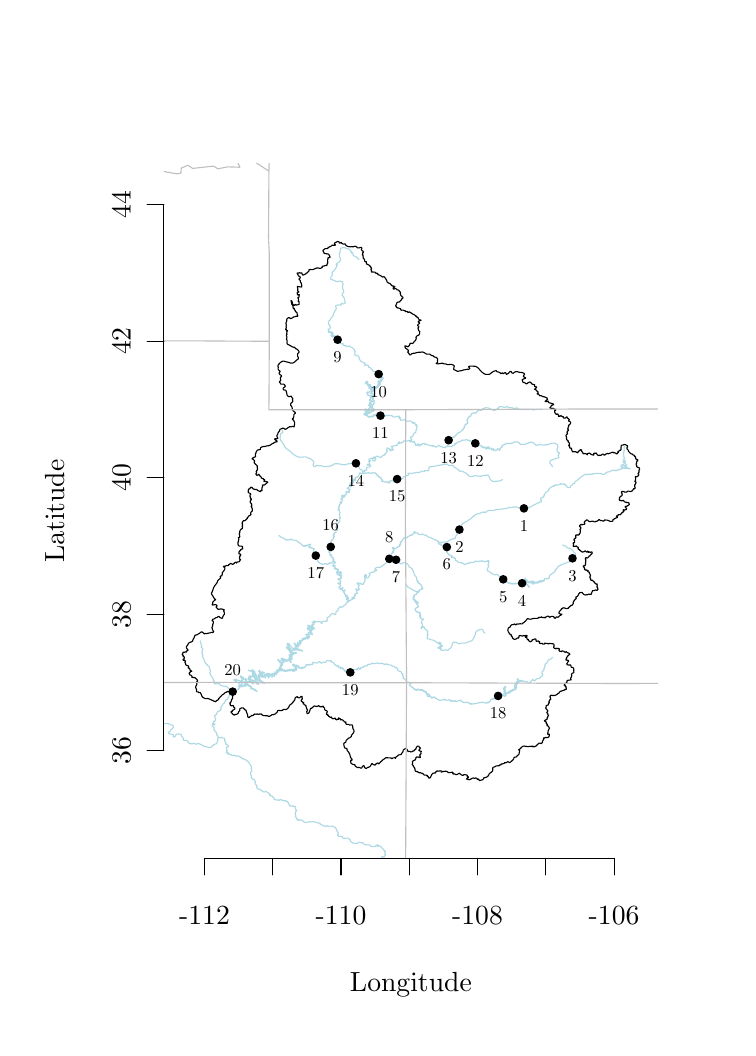
\begin{tikzpicture}[x=1pt,y=1pt]
\definecolor[named]{drawColor}{rgb}{0.00,0.00,0.00}
\definecolor[named]{fillColor}{rgb}{1.00,1.00,1.00}
\fill[color=fillColor,] (0,0) rectangle (252.94,361.35);
\begin{scope}
\path[clip] ( 49.20, 61.20) rectangle (227.75,312.15);

\draw[fill opacity=0.00,draw opacity=0.00,] ( 49.20, 61.20) rectangle (227.74,312.15);
\definecolor[named]{drawColor}{rgb}{0.00,0.00,0.00}

\draw[color=drawColor,line cap=round,line join=round,fill opacity=0.00,] (112.12,284.08) --
	(112.16,284.07) --
	(112.17,284.07) --
	(112.19,284.07) --
	(112.25,284.07) --
	(112.29,284.05) --
	(112.33,284.05) --
	(112.39,284.04) --
	(112.43,284.03) --
	(112.51,283.97) --
	(112.52,283.95) --
	(112.53,283.91) --
	(112.53,283.90) --
	(112.51,283.87) --
	(112.50,283.82) --
	(112.51,283.80) --
	(112.52,283.78) --
	(112.52,283.77) --
	(112.56,283.67) --
	(112.57,283.64) --
	(112.60,283.62) --
	(112.60,283.60) --
	(112.62,283.56) --
	(112.64,283.55) --
	(112.68,283.53) --
	(112.70,283.52) --
	(112.75,283.51) --
	(112.79,283.51) --
	(112.82,283.52) --
	(112.86,283.53) --
	(112.92,283.55) --
	(112.96,283.57) --
	(112.98,283.58) --
	(113.00,283.60) --
	(113.02,283.61) --
	(113.05,283.62) --
	(113.11,283.65) --
	(113.16,283.67) --
	(113.23,283.68) --
	(113.23,283.69) --
	(113.23,283.69) --
	(113.23,283.70) --
	(113.23,283.70) --
	(113.23,283.71) --
	(113.23,283.71) --
	(113.23,283.72) --
	(113.23,283.72) --
	(113.23,283.73) --
	(113.23,283.73) --
	(113.23,283.74) --
	(113.27,283.74) --
	(113.33,283.73) --
	(113.37,283.71) --
	(113.39,283.67) --
	(113.39,283.64) --
	(113.38,283.56) --
	(113.40,283.53) --
	(113.42,283.52) --
	(113.44,283.50) --
	(113.45,283.47) --
	(113.47,283.44) --
	(113.50,283.41) --
	(113.55,283.38) --
	(113.60,283.36) --
	(113.64,283.34) --
	(113.72,283.32) --
	(113.78,283.29) --
	(113.84,283.26) --
	(113.91,283.21) --
	(114.01,283.17) --
	(114.08,283.15) --
	(114.15,283.13) --
	(114.21,283.13) --
	(114.29,283.14) --
	(114.37,283.15) --
	(114.53,283.21) --
	(114.56,283.22) --
	(114.61,283.22) --
	(114.67,283.18) --
	(114.72,283.14) --
	(114.75,283.10) --
	(114.78,283.07) --
	(114.82,283.05) --
	(114.86,283.01) --
	(114.87,282.98) --
	(114.88,282.94) --
	(114.88,282.88) --
	(114.91,282.83) --
	(114.97,282.73) --
	(115.08,282.64) --
	(115.18,282.56) --
	(115.35,282.46) --
	(115.43,282.42) --
	(115.54,282.36) --
	(115.60,282.35) --
	(115.67,282.33) --
	(115.74,282.30) --
	(115.80,282.27) --
	(115.91,282.23) --
	(115.96,282.22) --
	(116.04,282.21) --
	(116.11,282.21) --
	(116.21,282.23) --
	(116.27,282.22) --
	(116.31,282.21) --
	(116.34,282.19) --
	(116.38,282.18) --
	(116.43,282.17) --
	(116.49,282.16) --
	(116.55,282.15) --
	(116.59,282.15) --
	(116.66,282.15) --
	(116.73,282.17) --
	(116.84,282.21) --
	(116.86,282.22) --
	(116.90,282.23) --
	(116.96,282.23) --
	(117.03,282.22) --
	(117.19,282.19) --
	(117.27,282.19) --
	(117.30,282.18) --
	(117.36,282.16) --
	(117.39,282.17) --
	(117.53,282.16) --
	(117.60,282.16) --
	(117.65,282.17) --
	(117.76,282.21) --
	(117.80,282.23) --
	(117.82,282.25) --
	(117.85,282.26) --
	(117.88,282.27) --
	(117.93,282.27) --
	(117.99,282.28) --
	(118.05,282.30) --
	(118.19,282.35) --
	(118.22,282.35) --
	(118.28,282.35) --
	(118.35,282.35) --
	(118.42,282.33) --
	(118.47,282.31) --
	(118.52,282.30) --
	(118.57,282.30) --
	(118.60,282.30) --
	(118.70,282.20) --
	(118.75,282.16) --
	(118.79,282.13) --
	(118.84,282.11) --
	(118.93,282.08) --
	(118.97,282.05) --
	(119.01,282.02) --
	(119.03,281.99) --
	(119.05,281.94) --
	(119.09,281.89) --
	(119.16,281.82) --
	(119.21,281.79) --
	(119.24,281.78) --
	(119.28,281.77) --
	(119.34,281.77) --
	(119.40,281.79) --
	(119.50,281.79) --
	(119.63,281.76) --
	(119.69,281.77) --
	(119.71,281.77) --
	(119.79,281.77) --
	(119.87,281.79) --
	(120.04,281.86) --
	(120.18,281.92) --
	(120.22,281.94) --
	(120.26,281.95) --
	(120.33,281.96) --
	(120.38,281.95) --
	(120.45,281.93) --
	(120.54,281.90) --
	(120.60,281.88) --
	(120.64,281.85) --
	(120.71,281.81) --
	(120.74,281.77) --
	(120.77,281.71) --
	(120.77,281.64) --
	(120.77,281.56) --
	(120.75,281.47) --
	(120.73,281.41) --
	(120.65,281.26) --
	(120.61,281.17) --
	(120.61,281.15) --
	(120.63,281.11) --
	(120.66,281.05) --
	(120.72,280.91) --
	(120.76,280.83) --
	(120.81,280.76) --
	(120.89,280.69) --
	(120.95,280.67) --
	(121.08,280.66) --
	(121.10,280.66) --
	(121.12,280.64) --
	(121.14,280.59) --
	(121.16,280.54) --
	(121.18,280.50) --
	(121.28,280.42) --
	(121.31,280.39) --
	(121.33,280.33) --
	(121.33,280.28) --
	(121.31,280.17) --
	(121.27,280.14) --
	(121.15,280.08) --
	(121.10,280.06) --
	(121.09,280.05) --
	(121.08,280.03) --
	(121.10,279.96) --
	(121.09,279.89) --
	(121.08,279.82) --
	(121.04,279.70) --
	(121.04,279.67) --
	(121.05,279.64) --
	(121.07,279.61) --
	(121.09,279.59) --
	(121.11,279.56) --
	(121.14,279.50) --
	(121.14,279.46) --
	(121.10,279.42) --
	(121.00,279.34) --
	(120.91,279.28) --
	(120.90,279.26) --
	(120.91,279.23) --
	(120.94,279.20) --
	(120.98,279.18) --
	(121.03,279.17) --
	(121.08,279.14) --
	(121.11,279.12) --
	(121.16,279.06) --
	(121.19,279.02) --
	(121.20,278.97) --
	(121.20,278.91) --
	(121.20,278.82) --
	(121.21,278.76) --
	(121.21,278.71) --
	(121.20,278.65) --
	(121.18,278.59) --
	(121.18,278.57) --
	(121.22,278.54) --
	(121.24,278.51) --
	(121.25,278.48) --
	(121.24,278.43) --
	(121.24,278.37) --
	(121.24,278.31) --
	(121.23,278.25) --
	(121.22,278.13) --
	(121.22,278.09) --
	(121.23,278.06) --
	(121.25,278.03) --
	(121.31,278.01) --
	(121.37,277.97) --
	(121.47,277.85) --
	(121.49,277.79) --
	(121.52,277.76) --
	(121.58,277.73) --
	(121.60,277.71) --
	(121.63,277.66) --
	(121.67,277.59) --
	(121.71,277.49) --
	(121.74,277.42) --
	(121.75,277.37) --
	(121.76,277.30) --
	(121.76,277.25) --
	(121.75,277.20) --
	(121.74,277.10) --
	(121.74,277.04) --
	(121.76,277.00) --
	(121.80,276.95) --
	(121.84,276.91) --
	(121.86,276.86) --
	(121.89,276.83) --
	(121.91,276.82) --
	(121.94,276.81) --
	(121.96,276.80) --
	(122.05,276.80) --
	(122.09,276.80) --
	(122.16,276.82) --
	(122.22,276.81) --
	(122.35,276.78) --
	(122.37,276.76) --
	(122.37,276.74) --
	(122.36,276.70) --
	(122.35,276.64) --
	(122.33,276.54) --
	(122.32,276.49) --
	(122.32,276.44) --
	(122.35,276.33) --
	(122.40,276.23) --
	(122.42,276.20) --
	(122.44,276.18) --
	(122.46,276.15) --
	(122.48,276.10) --
	(122.51,276.03) --
	(122.54,275.96) --
	(122.57,275.88) --
	(122.58,275.86) --
	(122.60,275.84) --
	(122.64,275.83) --
	(122.68,275.83) --
	(122.72,275.82) --
	(122.79,275.82) --
	(122.83,275.81) --
	(122.90,275.77) --
	(122.93,275.74) --
	(122.95,275.72) --
	(123.00,275.70) --
	(123.06,275.69) --
	(123.11,275.69) --
	(123.20,275.65) --
	(123.30,275.57) --
	(123.45,275.43) --
	(123.52,275.32) --
	(123.56,275.24) --
	(123.58,275.23) --
	(123.61,275.23) --
	(123.68,275.22) --
	(123.73,275.23) --
	(123.78,275.23) --
	(123.80,275.20) --
	(123.82,275.16) --
	(123.83,275.13) --
	(123.84,275.09) --
	(123.84,275.06) --
	(123.84,275.02) --
	(123.85,275.00) --
	(123.87,274.96) --
	(123.91,274.92) --
	(123.97,274.89) --
	(124.01,274.85) --
	(124.04,274.79) --
	(124.05,274.76) --
	(124.05,274.72) --
	(124.05,274.69) --
	(124.06,274.65) --
	(124.08,274.61) --
	(124.12,274.56) --
	(124.20,274.53) --
	(124.22,274.50) --
	(124.22,274.45) --
	(124.23,274.38) --
	(124.23,274.32) --
	(124.24,274.28) --
	(124.24,274.24) --
	(124.19,274.19) --
	(124.12,274.12) --
	(124.06,274.06) --
	(124.04,274.05) --
	(124.03,274.04) --
	(124.03,274.03) --
	(124.03,274.01) --
	(124.05,273.97) --
	(124.07,273.91) --
	(124.08,273.84) --
	(124.12,273.73) --
	(124.14,273.69) --
	(124.17,273.66) --
	(124.22,273.62) --
	(124.24,273.58) --
	(124.25,273.55) --
	(124.24,273.51) --
	(124.23,273.48) --
	(124.21,273.42) --
	(124.19,273.35) --
	(124.18,273.31) --
	(124.19,273.27) --
	(124.21,273.22) --
	(124.25,273.13) --
	(124.25,273.08) --
	(124.26,273.07) --
	(124.29,273.06) --
	(124.33,273.05) --
	(124.41,273.04) --
	(124.47,273.02) --
	(124.50,273.02) --
	(124.60,273.06) --
	(124.70,273.09) --
	(124.74,273.09) --
	(124.81,273.08) --
	(124.89,273.05) --
	(124.92,273.03) --
	(124.95,273.00) --
	(124.97,272.99) --
	(125.00,272.99) --
	(125.03,273.00) --
	(125.07,273.01) --
	(125.10,273.01) --
	(125.20,273.00) --
	(125.32,272.99) --
	(125.43,272.99) --
	(125.49,272.98) --
	(125.55,272.95) --
	(125.57,272.93) --
	(125.59,272.90) --
	(125.60,272.86) --
	(125.63,272.84) --
	(125.66,272.81) --
	(125.69,272.79) --
	(125.72,272.76) --
	(125.73,272.75) --
	(125.73,272.75) --
	(125.72,272.75) --
	(125.72,272.75) --
	(125.71,272.75) --
	(125.71,272.75) --
	(125.71,272.71) --
	(125.73,272.69) --
	(125.75,272.65) --
	(125.85,272.61) --
	(125.93,272.60) --
	(125.97,272.60) --
	(126.11,272.62) --
	(126.15,272.62) --
	(126.17,272.62) --
	(126.20,272.60) --
	(126.27,272.52) --
	(126.28,272.51) --
	(126.30,272.50) --
	(126.33,272.51) --
	(126.37,272.53) --
	(126.40,272.54) --
	(126.42,272.53) --
	(126.46,272.52) --
	(126.49,272.50) --
	(126.51,272.46) --
	(126.51,272.44) --
	(126.51,272.41) --
	(126.49,272.38) --
	(126.48,272.33) --
	(126.48,272.30) --
	(126.58,272.16) --
	(126.64,272.11) --
	(126.66,272.06) --
	(126.68,272.05) --
	(126.70,272.04) --
	(126.71,272.04) --
	(126.77,272.05) --
	(126.85,272.03) --
	(126.88,272.01) --
	(126.94,271.98) --
	(126.99,271.96) --
	(127.04,271.96) --
	(127.16,271.95) --
	(127.19,271.94) --
	(127.21,271.93) --
	(127.36,271.76) --
	(127.40,271.73) --
	(127.46,271.71) --
	(127.66,271.66) --
	(127.69,271.66) --
	(127.72,271.65) --
	(127.91,271.51) --
	(128.00,271.44) --
	(128.03,271.41) --
	(128.06,271.34) --
	(128.07,271.31) --
	(128.08,271.29) --
	(128.10,271.27) --
	(128.12,271.26) --
	(128.16,271.26) --
	(128.31,271.26) --
	(128.38,271.27) --
	(128.47,271.28) --
	(128.49,271.29) --
	(128.57,271.34) --
	(128.70,271.42) --
	(128.72,271.42) --
	(128.73,271.42) --
	(128.74,271.41) --
	(128.75,271.40) --
	(128.76,271.37) --
	(128.85,271.29) --
	(128.96,271.21) --
	(128.99,271.17) --
	(129.03,271.13) --
	(129.10,270.96) --
	(129.14,270.91) --
	(129.24,270.82) --
	(129.33,270.76) --
	(129.37,270.74) --
	(129.43,270.60) --
	(129.46,270.50) --
	(129.47,270.43) --
	(129.50,270.37) --
	(129.51,270.34) --
	(129.55,270.26) --
	(129.58,270.23) --
	(129.63,270.20) --
	(129.70,270.17) --
	(129.72,270.15) --
	(129.76,270.04) --
	(129.78,269.92) --
	(129.78,269.84) --
	(129.77,269.71) --
	(129.78,269.68) --
	(129.86,269.54) --
	(129.94,269.40) --
	(129.99,269.35) --
	(130.03,269.27) --
	(130.06,269.23) --
	(130.08,269.22) --
	(130.12,269.20) --
	(130.35,269.14) --
	(130.40,269.12) --
	(130.44,269.10) --
	(130.49,269.07) --
	(130.54,269.02) --
	(130.59,269.00) --
	(130.63,268.97) --
	(130.69,268.96) --
	(130.78,268.94) --
	(130.84,268.94) --
	(130.87,268.93) --
	(130.90,268.91) --
	(130.95,268.89) --
	(131.00,268.82) --
	(131.02,268.76) --
	(131.05,268.73) --
	(131.12,268.68) --
	(131.18,268.63) --
	(131.20,268.59) --
	(131.21,268.56) --
	(131.21,268.49) --
	(131.22,268.47) --
	(131.24,268.44) --
	(131.28,268.42) --
	(131.33,268.41) --
	(131.39,268.40) --
	(131.41,268.39) --
	(131.43,268.38) --
	(131.46,268.30) --
	(131.51,268.20) --
	(131.55,268.15) --
	(131.58,268.15) --
	(131.61,268.13) --
	(131.74,268.02) --
	(131.77,268.00) --
	(131.81,267.96) --
	(131.87,267.94) --
	(131.89,267.94) --
	(131.91,267.95) --
	(131.93,267.99) --
	(131.97,268.03) --
	(132.02,268.05) --
	(132.04,268.05) --
	(132.07,268.05) --
	(132.10,268.02) --
	(132.17,267.96) --
	(132.20,267.94) --
	(132.25,267.92) --
	(132.38,267.89) --
	(132.51,267.87) --
	(132.54,267.87) --
	(132.58,267.84) --
	(132.62,267.79) --
	(132.64,267.76) --
	(132.65,267.73) --
	(132.68,267.69) --
	(132.68,267.66) --
	(132.65,267.64) --
	(132.60,267.63) --
	(132.55,267.62) --
	(132.51,267.60) --
	(132.45,267.61) --
	(132.41,267.61) --
	(132.39,267.60) --
	(132.36,267.58) --
	(132.34,267.56) --
	(132.32,267.54) --
	(132.29,267.49) --
	(132.25,267.45) --
	(132.20,267.43) --
	(132.17,267.40) --
	(132.12,267.35) --
	(132.07,267.27) --
	(132.04,267.25) --
	(132.04,267.21) --
	(132.05,267.19) --
	(132.07,267.16) --
	(132.08,267.13) --
	(132.08,267.11) --
	(132.06,267.08) --
	(132.06,267.06) --
	(132.06,267.04) --
	(132.07,267.02) --
	(132.16,266.96) --
	(132.25,266.92) --
	(132.31,266.89) --
	(132.40,266.89) --
	(132.44,266.89) --
	(132.48,266.90) --
	(132.51,266.91) --
	(132.55,266.94) --
	(132.63,267.01) --
	(132.72,267.07) --
	(132.76,267.09) --
	(132.80,267.09) --
	(132.84,267.09) --
	(132.92,267.06) --
	(132.97,267.05) --
	(133.06,267.03) --
	(133.08,267.01) --
	(133.12,266.98) --
	(133.18,266.94) --
	(133.28,266.89) --
	(133.31,266.86) --
	(133.35,266.79) --
	(133.38,266.74) --
	(133.41,266.70) --
	(133.44,266.67) --
	(133.49,266.64) --
	(133.75,266.58) --
	(133.87,266.54) --
	(133.91,266.53) --
	(133.95,266.52) --
	(133.98,266.50) --
	(134.01,266.46) --
	(134.03,266.44) --
	(134.15,266.39) --
	(134.19,266.36) --
	(134.24,266.31) --
	(134.28,266.26) --
	(134.29,266.23) --
	(134.29,266.10) --
	(134.31,266.05) --
	(134.32,266.03) --
	(134.35,266.00) --
	(134.41,265.97) --
	(134.52,265.93) --
	(134.55,265.91) --
	(134.57,265.88) --
	(134.59,265.84) --
	(134.63,265.77) --
	(134.66,265.67) --
	(134.68,265.64) --
	(134.76,265.54) --
	(134.75,265.52) --
	(134.70,265.48) --
	(134.64,265.40) --
	(134.61,265.32) --
	(134.60,265.27) --
	(134.60,265.25) --
	(134.61,265.21) --
	(134.62,265.18) --
	(134.73,265.01) --
	(134.76,264.95) --
	(134.77,264.89) --
	(134.77,264.80) --
	(134.76,264.76) --
	(134.77,264.73) --
	(134.79,264.70) --
	(134.83,264.61) --
	(134.88,264.55) --
	(135.02,264.43) --
	(135.15,264.33) --
	(135.18,264.30) --
	(135.21,264.26) --
	(135.25,264.14) --
	(135.29,264.09) --
	(135.32,264.07) --
	(135.37,264.05) --
	(135.41,264.04) --
	(135.46,264.02) --
	(135.51,264.00) --
	(135.57,263.95) --
	(135.59,263.92) --
	(135.60,263.90) --
	(135.61,263.85) --
	(135.60,263.80) --
	(135.58,263.76) --
	(135.58,263.72) --
	(135.59,263.69) --
	(135.60,263.62) --
	(135.59,263.59) --
	(135.57,263.57) --
	(135.55,263.55) --
	(135.46,263.49) --
	(135.29,263.43) --
	(135.24,263.42) --
	(135.19,263.39) --
	(135.14,263.35) --
	(135.10,263.30) --
	(135.09,263.26) --
	(135.10,263.23) --
	(135.13,263.17) --
	(135.13,263.09) --
	(135.13,263.07) --
	(135.13,263.03) --
	(135.11,263.01) --
	(134.99,262.94) --
	(134.81,262.80) --
	(134.76,262.76) --
	(134.70,262.72) --
	(134.66,262.68) --
	(134.63,262.63) --
	(134.61,262.56) --
	(134.59,262.51) --
	(134.59,262.49) --
	(134.56,262.46) --
	(134.53,262.42) --
	(134.45,262.30) --
	(134.38,262.26) --
	(134.34,262.23) --
	(134.28,262.22) --
	(134.16,262.23) --
	(134.08,262.23) --
	(134.04,262.22) --
	(133.97,262.19) --
	(133.89,262.18) --
	(133.62,262.13) --
	(133.56,262.10) --
	(133.46,261.97) --
	(133.43,261.95) --
	(133.38,261.92) --
	(133.36,261.91) --
	(133.36,261.89) --
	(133.36,261.85) --
	(133.36,261.81) --
	(133.35,261.78) --
	(133.32,261.72) --
	(133.31,261.62) --
	(133.30,261.53) --
	(133.29,261.50) --
	(133.24,261.41) --
	(133.18,261.32) --
	(133.16,261.27) --
	(133.07,261.02) --
	(132.98,260.90) --
	(132.97,260.85) --
	(132.97,260.82) --
	(132.97,260.80) --
	(132.98,260.75) --
	(133.02,260.72) --
	(133.10,260.68) --
	(133.17,260.64) --
	(133.24,260.59) --
	(133.26,260.55) --
	(133.26,260.49) --
	(133.25,260.39) --
	(133.24,260.34) --
	(133.24,260.31) --
	(133.25,260.28) --
	(133.27,260.24) --
	(133.32,260.20) --
	(133.38,260.17) --
	(133.59,260.14) --
	(133.64,260.13) --
	(133.72,260.07) --
	(133.77,260.05) --
	(133.84,260.05) --
	(133.98,260.04) --
	(134.11,260.01) --
	(134.21,259.97) --
	(134.34,259.91) --
	(134.40,259.88) --
	(134.49,259.86) --
	(134.64,259.86) --
	(134.68,259.86) --
	(134.70,259.85) --
	(134.72,259.83) --
	(134.74,259.81) --
	(134.80,259.64) --
	(134.81,259.59) --
	(134.82,259.55) --
	(134.81,259.52) --
	(134.80,259.49) --
	(134.80,259.46) --
	(134.85,259.40) --
	(134.89,259.32) --
	(134.91,259.29) --
	(134.95,259.27) --
	(135.01,259.25) --
	(135.07,259.25) --
	(135.14,259.26) --
	(135.25,259.30) --
	(135.29,259.30) --
	(135.33,259.30) --
	(135.47,259.27) --
	(135.54,259.27) --
	(135.57,259.27) --
	(135.65,259.30) --
	(135.69,259.30) --
	(135.72,259.30) --
	(135.76,259.29) --
	(135.79,259.28) --
	(135.86,259.20) --
	(135.91,259.17) --
	(135.96,259.15) --
	(136.03,259.14) --
	(136.20,259.12) --
	(136.35,259.09) --
	(136.39,259.07) --
	(136.46,259.03) --
	(136.46,259.00) --
	(136.47,258.94) --
	(136.45,258.87) --
	(136.43,258.82) --
	(136.44,258.80) --
	(136.50,258.78) --
	(136.57,258.77) --
	(136.65,258.79) --
	(136.73,258.81) --
	(136.78,258.80) --
	(136.82,258.79) --
	(136.89,258.80) --
	(136.94,258.81) --
	(137.05,258.82) --
	(137.10,258.82) --
	(137.15,258.80) --
	(137.18,258.78) --
	(137.26,258.71) --
	(137.31,258.64) --
	(137.34,258.49) --
	(137.36,258.47) --
	(137.39,258.47) --
	(137.43,258.48) --
	(137.47,258.47) --
	(137.54,258.48) --
	(137.57,258.49) --
	(137.67,258.53) --
	(137.80,258.60) --
	(137.83,258.62) --
	(137.85,258.65) --
	(137.86,258.66) --
	(137.88,258.67) --
	(138.06,258.65) --
	(138.10,258.63) --
	(138.12,258.62) --
	(138.14,258.50) --
	(138.16,258.45) --
	(138.16,258.41) --
	(138.18,258.38) --
	(138.21,258.36) --
	(138.26,258.35) --
	(138.34,258.34) --
	(138.39,258.34) --
	(138.47,258.33) --
	(138.55,258.31) --
	(138.63,258.28) --
	(138.65,258.27) --
	(138.74,258.16) --
	(138.85,258.07) --
	(139.14,257.86) --
	(139.38,257.74) --
	(139.48,257.72) --
	(139.52,257.70) --
	(139.60,257.65) --
	(139.66,257.62) --
	(139.74,257.57) --
	(139.80,257.54) --
	(140.07,257.35) --
	(140.35,257.16) --
	(140.43,257.10) --
	(140.48,257.05) --
	(140.50,257.03) --
	(140.50,257.01) --
	(140.49,257.00) --
	(140.46,256.98) --
	(140.41,256.97) --
	(140.35,256.97) --
	(140.31,256.97) --
	(140.30,256.96) --
	(140.29,256.93) --
	(140.30,256.91) --
	(140.33,256.89) --
	(140.38,256.87) --
	(140.62,256.78) --
	(140.83,256.71) --
	(140.91,256.68) --
	(140.97,256.66) --
	(141.02,256.63) --
	(141.10,256.54) --
	(141.13,256.45) --
	(141.13,256.35) --
	(141.15,256.29) --
	(141.19,256.21) --
	(141.23,256.14) --
	(141.29,256.06) --
	(141.39,255.94) --
	(141.43,255.88) --
	(141.46,255.84) --
	(141.49,255.81) --
	(141.53,255.78) --
	(141.56,255.76) --
	(141.62,255.75) --
	(141.72,255.75) --
	(141.90,255.75) --
	(141.97,255.73) --
	(142.06,255.68) --
	(142.12,255.63) --
	(142.13,255.62) --
	(142.13,255.59) --
	(142.10,255.57) --
	(142.03,255.56) --
	(141.91,255.53) --
	(141.74,255.46) --
	(141.65,255.41) --
	(141.59,255.38) --
	(141.51,255.36) --
	(141.34,255.30) --
	(141.22,255.23) --
	(141.15,255.15) --
	(141.13,255.10) --
	(141.12,255.06) --
	(141.12,255.03) --
	(141.15,255.01) --
	(141.21,254.98) --
	(141.28,254.95) --
	(141.33,254.91) --
	(141.37,254.85) --
	(141.42,254.81) --
	(141.47,254.76) --
	(141.55,254.70) --
	(141.57,254.68) --
	(141.59,254.65) --
	(141.60,254.62) --
	(141.62,254.57) --
	(141.62,254.53) --
	(141.63,254.51) --
	(141.58,254.48) --
	(141.52,254.43) --
	(141.48,254.39) --
	(141.30,254.28) --
	(141.23,254.22) --
	(141.17,254.14) --
	(141.02,254.03) --
	(140.98,253.98) --
	(140.96,253.94) --
	(140.96,253.92) --
	(140.96,253.88) --
	(140.99,253.83) --
	(140.99,253.82) --
	(140.98,253.79) --
	(140.95,253.76) --
	(140.95,253.69) --
	(140.95,253.66) --
	(140.97,253.63) --
	(141.00,253.60) --
	(141.11,253.52) --
	(141.23,253.42) --
	(141.29,253.37) --
	(141.31,253.34) --
	(141.32,253.31) --
	(141.32,253.25) --
	(141.31,253.17) --
	(141.29,253.12) --
	(141.26,253.07) --
	(141.24,253.03) --
	(141.21,252.99) --
	(141.14,252.91) --
	(141.10,252.89) --
	(141.08,252.87) --
	(141.05,252.83) --
	(141.04,252.81) --
	(141.04,252.78) --
	(141.07,252.66) --
	(141.11,252.53) --
	(141.13,252.48) --
	(141.15,252.32) --
	(141.18,252.22) --
	(141.23,252.05) --
	(141.28,251.92) --
	(141.33,251.85) --
	(141.42,251.76) --
	(141.50,251.70) --
	(141.55,251.65) --
	(141.65,251.59) --
	(141.67,251.57) --
	(141.69,251.56) --
	(141.69,251.49) --
	(141.70,251.45) --
	(141.68,251.40) --
	(141.66,251.35) --
	(141.65,251.29) --
	(141.63,251.21) --
	(141.63,250.92) --
	(141.62,250.84) --
	(141.62,250.71) --
	(141.61,250.63) --
	(141.59,250.60) --
	(141.43,250.43) --
	(141.39,250.38) --
	(141.37,250.34) --
	(141.35,250.31) --
	(141.29,250.26) --
	(141.22,250.21) --
	(141.16,250.18) --
	(140.91,250.07) --
	(140.81,250.03) --
	(140.74,249.98) --
	(140.60,249.89) --
	(140.56,249.84) --
	(140.53,249.80) --
	(140.47,249.73) --
	(140.40,249.60) --
	(140.34,249.48) --
	(140.30,249.34) --
	(140.30,249.29) --
	(140.30,249.26) --
	(140.32,249.24) --
	(140.37,249.18) --
	(140.41,249.13) --
	(140.42,249.10) --
	(140.42,249.05) --
	(140.39,248.99) --
	(140.37,248.94) --
	(140.36,248.90) --
	(140.32,248.69) --
	(140.29,248.62) --
	(140.26,248.58) --
	(140.21,248.48) --
	(140.17,248.39) --
	(139.91,248.08) --
	(139.90,248.08) --
	(139.90,248.08) --
	(139.89,248.08) --
	(139.89,248.08) --
	(139.88,248.08) --
	(139.88,248.08) --
	(139.87,248.08) --
	(139.87,248.08) --
	(139.86,248.08) --
	(139.86,248.08) --
	(139.85,248.08) --
	(139.85,248.08) --
	(139.84,248.08) --
	(139.84,248.08) --
	(139.83,248.08) --
	(139.82,248.07) --
	(139.64,247.97) --
	(139.62,247.88) --
	(139.61,247.86) --
	(139.59,247.76) --
	(139.56,247.68) --
	(139.53,247.65) --
	(139.50,247.61) --
	(139.50,247.59) --
	(139.48,247.59) --
	(139.44,247.55) --
	(139.39,247.50) --
	(139.37,247.49) --
	(139.35,247.47) --
	(139.33,247.45) --
	(139.32,247.43) --
	(139.30,247.37) --
	(139.24,247.33) --
	(139.17,247.29) --
	(139.08,247.25) --
	(139.00,247.23) --
	(138.97,247.23) --
	(138.92,247.24) --
	(138.89,247.24) --
	(138.87,247.26) --
	(138.76,247.26) --
	(138.70,247.26) --
	(138.67,247.26) --
	(138.60,247.28) --
	(138.55,247.31) --
	(138.44,247.32) --
	(138.41,247.31) --
	(138.39,247.30) --
	(138.34,247.28) --
	(138.31,247.24) --
	(138.27,247.21) --
	(138.21,247.18) --
	(138.18,247.17) --
	(138.11,247.16) --
	(138.09,247.13) --
	(138.08,247.11) --
	(138.08,246.91) --
	(138.06,246.78) --
	(138.02,246.67) --
	(137.97,246.58) --
	(137.91,246.50) --
	(137.85,246.44) --
	(137.72,246.34) --
	(137.63,246.26) --
	(137.61,246.25) --
	(137.60,246.23) --
	(137.48,246.09) --
	(137.46,246.08) --
	(137.44,246.06) --
	(137.38,246.05) --
	(137.33,246.05) --
	(137.30,246.05) --
	(137.22,246.08) --
	(137.18,246.10) --
	(137.15,246.11) --
	(137.06,246.15) --
	(136.97,246.20) --
	(136.71,246.30) --
	(136.56,246.34) --
	(136.37,246.38) --
	(136.31,246.36) --
	(136.30,246.35) --
	(136.29,246.33) --
	(136.30,246.27) --
	(136.33,246.19) --
	(136.33,246.17) --
	(136.33,246.12) --
	(136.33,246.06) --
	(136.33,246.02) --
	(136.33,245.98) --
	(136.34,245.94) --
	(136.36,245.84) --
	(136.38,245.80) --
	(136.42,245.72) --
	(136.45,245.67) --
	(136.57,245.55) --
	(136.59,245.52) --
	(136.61,245.51) --
	(136.61,245.49) --
	(136.63,245.47) --
	(136.69,245.42) --
	(136.72,245.39) --
	(136.77,245.37) --
	(136.88,245.31) --
	(136.92,245.28) --
	(136.98,245.24) --
	(137.04,245.21) --
	(137.07,245.19) --
	(137.14,245.12) --
	(137.25,245.05) --
	(137.36,244.96) --
	(137.43,244.90) --
	(137.46,244.84) --
	(137.47,244.78) --
	(137.48,244.72) --
	(137.50,244.70) --
	(137.57,244.64) --
	(137.59,244.61) --
	(137.59,244.60) --
	(137.59,244.59) --
	(137.59,244.57) --
	(137.52,244.41) --
	(137.50,244.40) --
	(137.50,244.37) --
	(137.49,244.36) --
	(137.47,244.34) --
	(137.45,244.30) --
	(137.43,244.29) --
	(137.39,244.23) --
	(137.37,244.22) --
	(137.34,244.18) --
	(137.34,244.13) --
	(137.34,244.13) --
	(137.36,244.09) --
	(137.39,244.03) --
	(137.43,244.00) --
	(137.47,243.95) --
	(137.53,243.88) --
	(137.64,243.77) --
	(137.69,243.72) --
	(137.76,243.65) --
	(137.79,243.60) --
	(137.81,243.53) --
	(137.82,243.52) --
	(137.84,243.50) --
	(137.84,243.48) --
	(137.89,243.39) --
	(137.94,243.29) --
	(137.94,243.27) --
	(137.95,243.23) --
	(137.97,243.19) --
	(138.02,243.14) --
	(138.07,243.12) --
	(138.10,243.11) --
	(138.13,243.11) --
	(138.29,243.13) --
	(138.42,243.15) --
	(138.44,243.16) --
	(138.46,243.18) --
	(138.49,243.22) --
	(138.51,243.26) --
	(138.54,243.29) --
	(138.56,243.31) --
	(138.58,243.33) --
	(138.62,243.38) --
	(138.63,243.40) --
	(138.65,243.42) --
	(138.67,243.46) --
	(138.70,243.47) --
	(138.74,243.52) --
	(138.77,243.54) --
	(138.85,243.55) --
	(138.90,243.55) --
	(138.96,243.55) --
	(138.99,243.56) --
	(139.01,243.57) --
	(139.04,243.60) --
	(139.16,243.65) --
	(139.22,243.67) --
	(139.29,243.68) --
	(139.46,243.69) --
	(139.81,243.72) --
	(139.92,243.74) --
	(139.94,243.74) --
	(140.00,243.75) --
	(140.11,243.78) --
	(140.16,243.78) --
	(140.19,243.79) --
	(140.22,243.79) --
	(140.24,243.81) --
	(140.29,243.82) --
	(140.39,243.85) --
	(140.53,243.92) --
	(140.57,243.94) --
	(140.65,243.97) --
	(140.72,244.00) --
	(140.80,244.01) --
	(140.93,244.03) --
	(141.34,244.05) --
	(141.50,244.05) --
	(141.61,244.05) --
	(141.97,244.07) --
	(142.05,244.08) --
	(142.22,244.10) --
	(142.34,244.13) --
	(142.37,244.13) --
	(142.39,244.14) --
	(142.53,244.15) --
	(142.62,244.15) --
	(142.70,244.14) --
	(142.78,244.12) --
	(142.90,244.08) --
	(142.99,244.05) --
	(143.14,243.97) --
	(143.21,243.93) --
	(143.25,243.91) --
	(143.48,243.79) --
	(143.63,243.70) --
	(143.71,243.64) --
	(143.77,243.60) --
	(143.80,243.59) --
	(143.91,243.52) --
	(143.95,243.50) --
	(144.10,243.42) --
	(144.15,243.40) --
	(144.20,243.38) --
	(144.28,243.36) --
	(144.50,243.36) --
	(144.56,243.36) --
	(144.67,243.36) --
	(144.86,243.36) --
	(144.91,243.36) --
	(144.99,243.38) --
	(145.16,243.39) --
	(145.21,243.39) --
	(145.32,243.37) --
	(145.36,243.35) --
	(145.40,243.32) --
	(145.46,243.28) --
	(145.47,243.26) --
	(145.51,243.23) --
	(145.60,243.14) --
	(145.62,243.12) --
	(145.63,243.11) --
	(145.73,243.03) --
	(145.78,243.00) --
	(145.78,242.99) --
	(145.78,242.99) --
	(145.80,242.97) --
	(145.84,242.95) --
	(145.87,242.94) --
	(145.89,242.93) --
	(145.97,242.90) --
	(146.02,242.88) --
	(146.04,242.88) --
	(146.06,242.86) --
	(146.16,242.83) --
	(146.24,242.81) --
	(146.27,242.80) --
	(146.37,242.79) --
	(146.46,242.79) --
	(146.48,242.78) --
	(146.50,242.77) --
	(146.56,242.73) --
	(146.61,242.68) --
	(146.64,242.64) --
	(146.68,242.57) --
	(146.69,242.55) --
	(146.72,242.51) --
	(146.80,242.46) --
	(146.87,242.42) --
	(147.06,242.35) --
	(147.30,242.29) --
	(147.32,242.28) --
	(147.40,242.25) --
	(147.43,242.24) --
	(147.53,242.20) --
	(147.56,242.19) --
	(147.60,242.17) --
	(147.64,242.14) --
	(147.71,242.11) --
	(147.78,242.07) --
	(147.84,242.03) --
	(147.98,241.91) --
	(147.99,241.89) --
	(148.01,241.87) --
	(148.06,241.80) --
	(148.11,241.70) --
	(148.11,241.68) --
	(148.13,241.64) --
	(148.14,241.61) --
	(148.14,241.57) --
	(148.14,241.50) --
	(148.11,241.36) --
	(148.07,241.12) --
	(148.07,241.10) --
	(148.07,240.93) --
	(148.07,240.85) --
	(148.07,240.83) --
	(148.08,240.81) --
	(148.09,240.77) --
	(148.10,240.73) --
	(148.11,240.68) --
	(148.12,240.47) --
	(148.12,240.43) --
	(148.10,240.41) --
	(147.99,240.32) --
	(147.95,240.29) --
	(147.91,240.26) --
	(147.83,240.21) --
	(147.74,240.15) --
	(147.68,240.12) --
	(147.66,240.10) --
	(147.64,240.08) --
	(147.64,240.04) --
	(147.65,240.02) --
	(147.66,240.00) --
	(147.67,239.99) --
	(147.72,239.97) --
	(147.78,239.95) --
	(147.80,239.94) --
	(147.90,239.91) --
	(148.11,239.88) --
	(148.17,239.88) --
	(148.22,239.87) --
	(148.33,239.88) --
	(148.42,239.89) --
	(148.55,239.91) --
	(148.82,239.94) --
	(148.98,239.97) --
	(149.37,240.05) --
	(149.51,240.07) --
	(149.61,240.09) --
	(149.69,240.10) --
	(149.81,240.10) --
	(149.86,240.09) --
	(150.09,240.05) --
	(150.12,240.04) --
	(150.21,240.01) --
	(150.24,240.00) --
	(150.29,239.98) --
	(150.31,239.94) --
	(150.35,239.91) --
	(150.41,239.87) --
	(150.43,239.86) --
	(150.51,239.84) --
	(150.57,239.83) --
	(150.78,239.86) --
	(150.84,239.86) --
	(150.95,239.85) --
	(151.00,239.84) --
	(151.08,239.82) --
	(151.20,239.78) --
	(151.34,239.72) --
	(151.39,239.69) --
	(151.41,239.69) --
	(151.43,239.68) --
	(151.56,239.64) --
	(151.69,239.61) --
	(151.79,239.59) --
	(151.96,239.57) --
	(152.10,239.57) --
	(152.12,239.57) --
	(152.15,239.57) --
	(152.25,239.59) --
	(152.31,239.61) --
	(152.59,239.67) --
	(152.70,239.68) --
	(152.72,239.68) --
	(152.73,239.68) --
	(152.78,239.69) --
	(152.84,239.69) --
	(152.85,239.68) --
	(152.88,239.68) --
	(152.92,239.69) --
	(153.01,239.67) --
	(153.09,239.66) --
	(153.14,239.65) --
	(153.16,239.65) --
	(153.19,239.64) --
	(153.24,239.62) --
	(153.29,239.61) --
	(153.32,239.60) --
	(153.39,239.58) --
	(153.47,239.55) --
	(153.59,239.51) --
	(153.69,239.48) --
	(153.79,239.44) --
	(153.86,239.41) --
	(153.93,239.38) --
	(153.94,239.36) --
	(153.98,239.33) --
	(154.02,239.30) --
	(154.03,239.26) --
	(154.09,239.19) --
	(154.12,239.11) --
	(154.14,239.03) --
	(154.14,238.99) --
	(154.12,238.91) --
	(154.09,238.86) --
	(154.04,238.76) --
	(154.04,238.72) --
	(154.02,238.66) --
	(154.03,238.62) --
	(154.03,238.59) --
	(154.03,238.46) --
	(154.04,238.43) --
	(154.03,238.39) --
	(154.03,238.36) --
	(153.99,238.24) --
	(153.96,238.15) --
	(153.95,237.99) --
	(153.95,237.97) --
	(153.96,237.93) --
	(153.98,237.83) --
	(154.01,237.80) --
	(154.07,237.75) --
	(154.24,237.69) --
	(154.39,237.63) --
	(154.54,237.56) --
	(154.59,237.54) --
	(154.65,237.50) --
	(154.83,237.40) --
	(154.96,237.33) --
	(155.03,237.30) --
	(155.10,237.27) --
	(155.15,237.25) --
	(155.18,237.23) --
	(155.21,237.22) --
	(155.23,237.22) --
	(155.25,237.20) --
	(155.33,237.16) --
	(155.34,237.16) --
	(155.39,237.17) --
	(155.47,237.18) --
	(155.69,237.23) --
	(155.71,237.24) --
	(155.74,237.24) --
	(155.79,237.25) --
	(155.84,237.25) --
	(155.87,237.25) --
	(155.94,237.27) --
	(156.02,237.29) --
	(156.04,237.30) --
	(156.15,237.33) --
	(156.33,237.35) --
	(156.41,237.37) --
	(156.50,237.38) --
	(156.63,237.39) --
	(156.68,237.40) --
	(156.73,237.42) --
	(156.83,237.44) --
	(156.88,237.46) --
	(156.94,237.48) --
	(157.11,237.53) --
	(157.15,237.56) --
	(157.18,237.56) --
	(157.23,237.58) --
	(157.35,237.62) --
	(157.59,237.67) --
	(157.62,237.68) --
	(157.69,237.69) --
	(157.78,237.70) --
	(157.81,237.70) --
	(157.94,237.72) --
	(158.15,237.77) --
	(158.26,237.79) --
	(158.31,237.80) --
	(158.34,237.80) --
	(158.39,237.82) --
	(158.62,237.86) --
	(158.81,237.90) --
	(158.89,237.91) --
	(158.95,237.90) --
	(159.03,237.90) --
	(159.08,237.89) --
	(159.16,237.89) --
	(159.22,237.89) --
	(159.33,237.90) --
	(159.35,237.90) --
	(159.43,237.93) --
	(159.52,238.00) --
	(159.54,238.02) --
	(159.58,238.04) --
	(159.62,238.08) --
	(159.64,238.09) --
	(159.69,238.14) --
	(159.72,238.17) --
	(159.74,238.21) --
	(159.74,238.27) --
	(159.71,238.31) --
	(159.69,238.35) --
	(159.68,238.37) --
	(159.57,238.46) --
	(159.56,238.48) --
	(159.55,238.49) --
	(159.54,238.50) --
	(159.48,238.57) --
	(159.47,238.59) --
	(159.44,238.62) --
	(159.37,238.71) --
	(159.35,238.76) --
	(159.36,238.78) --
	(159.37,238.85) --
	(159.40,238.88) --
	(159.51,238.94) --
	(159.58,238.97) --
	(159.71,239.01) --
	(159.85,239.03) --
	(160.03,239.04) --
	(160.20,239.05) --
	(160.45,239.05) --
	(160.53,239.05) --
	(160.55,239.05) --
	(160.66,239.05) --
	(160.80,239.06) --
	(160.99,239.05) --
	(161.12,239.03) --
	(161.20,239.02) --
	(161.26,239.02) --
	(161.34,239.03) --
	(161.45,239.02) --
	(161.66,238.99) --
	(161.77,238.97) --
	(161.82,238.96) --
	(162.05,238.89) --
	(162.10,238.87) --
	(162.18,238.82) --
	(162.29,238.73) --
	(162.51,238.55) --
	(162.54,238.54) --
	(162.56,238.53) --
	(162.56,238.53) --
	(162.56,238.54) --
	(162.56,238.54) --
	(162.56,238.55) --
	(162.58,238.53) --
	(162.62,238.48) --
	(162.75,238.38) --
	(162.78,238.34) --
	(162.87,238.26) --
	(163.09,238.08) --
	(163.14,238.01) --
	(163.16,237.97) --
	(163.18,237.96) --
	(163.31,237.76) --
	(163.40,237.66) --
	(163.48,237.60) --
	(163.72,237.35) --
	(163.75,237.32) --
	(163.87,237.18) --
	(163.99,237.07) --
	(164.03,237.02) --
	(164.10,236.94) --
	(164.12,236.92) --
	(164.15,236.89) --
	(164.25,236.79) --
	(164.38,236.69) --
	(164.47,236.64) --
	(164.57,236.57) --
	(164.59,236.56) --
	(164.64,236.48) --
	(164.67,236.45) --
	(164.78,236.36) --
	(164.85,236.32) --
	(164.92,236.29) --
	(165.16,236.21) --
	(165.19,236.20) --
	(165.27,236.15) --
	(165.33,236.11) --
	(165.41,236.09) --
	(165.46,236.07) --
	(165.51,236.07) --
	(165.60,236.07) --
	(165.68,236.07) --
	(165.84,236.07) --
	(165.95,236.06) --
	(166.16,236.06) --
	(166.22,236.05) --
	(166.35,236.05) --
	(166.41,236.06) --
	(166.44,236.06) --
	(166.46,236.06) --
	(166.62,236.08) --
	(166.73,236.10) --
	(166.83,236.12) --
	(166.93,236.16) --
	(166.98,236.17) --
	(167.17,236.25) --
	(167.25,236.30) --
	(167.29,236.33) --
	(167.37,236.42) --
	(167.42,236.47) --
	(167.44,236.51) --
	(167.45,236.52) --
	(167.47,236.54) --
	(167.51,236.59) --
	(167.59,236.67) --
	(167.63,236.70) --
	(167.64,236.72) --
	(167.67,236.73) --
	(167.78,236.82) --
	(167.81,236.83) --
	(167.82,236.85) --
	(167.85,236.86) --
	(167.90,236.88) --
	(167.92,236.89) --
	(168.01,236.94) --
	(168.05,236.97) --
	(168.12,237.00) --
	(168.16,237.02) --
	(168.19,237.03) --
	(168.24,237.05) --
	(168.40,237.16) --
	(168.58,237.25) --
	(168.71,237.29) --
	(168.78,237.31) --
	(168.96,237.35) --
	(168.99,237.36) --
	(169.02,237.36) --
	(169.04,237.37) --
	(169.07,237.38) --
	(169.10,237.39) --
	(169.23,237.42) --
	(169.25,237.42) --
	(169.28,237.43) --
	(169.33,237.44) --
	(169.35,237.43) --
	(169.40,237.34) --
	(169.44,237.26) --
	(169.44,237.24) --
	(169.48,237.14) --
	(169.51,237.11) --
	(169.52,237.08) --
	(169.54,237.07) --
	(169.57,237.04) --
	(169.61,237.01) --
	(169.66,236.99) --
	(169.70,236.97) --
	(169.76,236.96) --
	(169.98,236.94) --
	(170.03,236.93) --
	(170.11,236.91) --
	(170.15,236.90) --
	(170.37,236.81) --
	(170.52,236.77) --
	(170.57,236.75) --
	(170.66,236.70) --
	(170.69,236.67) --
	(170.71,236.63) --
	(170.74,236.53) --
	(170.75,236.51) --
	(170.76,236.47) --
	(170.77,236.46) --
	(170.79,236.45) --
	(170.80,236.43) --
	(170.85,236.41) --
	(170.87,236.40) --
	(170.95,236.39) --
	(171.04,236.40) --
	(171.19,236.45) --
	(171.24,236.47) --
	(171.32,236.52) --
	(171.37,236.54) --
	(171.47,236.58) --
	(171.52,236.59) --
	(171.57,236.59) --
	(171.61,236.58) --
	(171.63,236.57) --
	(171.66,236.54) --
	(171.69,236.42) --
	(171.69,236.35) --
	(171.70,236.34) --
	(171.74,236.33) --
	(171.82,236.32) --
	(171.85,236.33) --
	(171.90,236.35) --
	(172.14,236.50) --
	(172.19,236.53) --
	(172.25,236.57) --
	(172.29,236.59) --
	(172.40,236.65) --
	(172.45,236.67) --
	(172.53,236.70) --
	(172.58,236.70) --
	(172.64,236.70) --
	(172.66,236.70) --
	(172.71,236.68) --
	(172.74,236.67) --
	(172.77,236.64) --
	(172.79,236.50) --
	(172.84,236.38) --
	(172.85,236.36) --
	(172.88,236.33) --
	(172.88,236.30) --
	(172.93,236.23) --
	(172.94,236.19) --
	(173.06,236.08) --
	(173.08,236.07) --
	(173.11,236.08) --
	(173.13,236.10) --
	(173.16,236.13) --
	(173.22,236.17) --
	(173.25,236.19) --
	(173.30,236.24) --
	(173.34,236.26) --
	(173.39,236.28) --
	(173.44,236.30) --
	(173.56,236.33) --
	(173.69,236.40) --
	(173.73,236.42) --
	(173.77,236.45) --
	(173.84,236.52) --
	(173.87,236.57) --
	(173.88,236.59) --
	(173.93,236.70) --
	(173.97,236.78) --
	(174.02,236.86) --
	(174.18,237.00) --
	(174.24,237.04) --
	(174.27,237.05) --
	(174.29,237.06) --
	(174.31,237.07) --
	(174.34,237.08) --
	(174.41,237.10) --
	(174.46,237.11) --
	(174.55,237.13) --
	(174.60,237.13) --
	(174.62,237.13) --
	(174.65,237.11) --
	(174.66,237.09) --
	(174.71,236.98) --
	(174.72,236.96) --
	(174.73,236.94) --
	(174.80,236.85) --
	(174.82,236.81) --
	(174.85,236.78) --
	(174.90,236.73) --
	(174.94,236.70) --
	(175.03,236.63) --
	(175.07,236.55) --
	(175.09,236.54) --
	(175.11,236.52) --
	(175.16,236.51) --
	(175.19,236.51) --
	(175.24,236.50) --
	(175.35,236.45) --
	(175.36,236.45) --
	(175.40,236.45) --
	(175.44,236.47) --
	(175.49,236.50) --
	(175.63,236.59) --
	(175.73,236.66) --
	(175.76,236.69) --
	(175.79,236.75) --
	(175.82,236.79) --
	(175.90,236.85) --
	(175.94,236.87) --
	(175.97,236.91) --
	(176.00,236.92) --
	(176.02,236.93) --
	(176.09,236.96) --
	(176.20,236.99) --
	(176.31,237.00) --
	(176.39,237.01) --
	(176.43,237.03) --
	(176.49,237.03) --
	(176.57,237.04) --
	(176.57,237.04) --
	(176.60,237.04) --
	(176.66,237.04) --
	(176.68,237.04) --
	(176.76,237.05) --
	(176.84,237.07) --
	(176.93,237.07) --
	(176.98,237.07) --
	(177.01,237.06) --
	(177.04,237.06) --
	(177.06,237.05) --
	(177.13,237.03) --
	(177.15,237.01) --
	(177.16,236.99) --
	(177.17,236.97) --
	(177.19,236.95) --
	(177.21,236.94) --
	(177.28,236.91) --
	(177.31,236.91) --
	(177.47,236.87) --
	(177.59,236.83) --
	(177.75,236.81) --
	(177.78,236.81) --
	(177.83,236.80) --
	(178.00,236.81) --
	(178.13,236.79) --
	(178.13,236.79) --
	(178.23,236.77) --
	(178.32,236.76) --
	(178.37,236.76) --
	(178.48,236.75) --
	(178.50,236.75) --
	(178.61,236.74) --
	(178.67,236.73) --
	(178.71,236.72) --
	(178.78,236.68) --
	(178.80,236.67) --
	(178.95,236.61) --
	(179.00,236.60) --
	(179.24,236.50) --
	(179.27,236.47) --
	(179.32,236.44) --
	(179.42,236.35) --
	(179.43,236.33) --
	(179.51,236.20) --
	(179.53,236.17) --
	(179.53,236.16) --
	(179.53,236.11) --
	(179.52,236.07) --
	(179.46,235.98) --
	(179.44,235.94) --
	(179.38,235.85) --
	(179.31,235.79) --
	(179.24,235.73) --
	(179.20,235.67) --
	(179.19,235.65) --
	(179.18,235.61) --
	(179.17,235.55) --
	(179.15,235.49) --
	(179.15,235.47) --
	(179.15,235.45) --
	(179.14,235.43) --
	(179.14,235.39) --
	(179.16,235.35) --
	(179.17,235.31) --
	(179.18,235.29) --
	(179.22,235.23) --
	(179.24,235.20) --
	(179.28,235.17) --
	(179.42,235.07) --
	(179.44,235.06) --
	(179.57,235.03) --
	(179.62,235.02) --
	(179.65,235.01) --
	(179.67,235.00) --
	(179.78,234.94) --
	(179.85,234.91) --
	(179.89,234.88) --
	(179.90,234.86) --
	(179.92,234.82) --
	(179.93,234.78) --
	(179.94,234.76) --
	(179.94,234.74) --
	(179.93,234.70) --
	(179.91,234.66) --
	(179.89,234.65) --
	(179.87,234.63) --
	(179.80,234.61) --
	(179.70,234.58) --
	(179.62,234.56) --
	(179.59,234.55) --
	(179.50,234.51) --
	(179.45,234.50) --
	(179.40,234.48) --
	(179.37,234.47) --
	(179.22,234.42) --
	(179.14,234.39) --
	(179.08,234.35) --
	(179.04,234.32) --
	(179.02,234.29) --
	(178.98,234.26) --
	(178.97,234.24) --
	(178.94,234.20) --
	(178.91,234.19) --
	(178.81,234.18) --
	(178.73,234.17) --
	(178.71,234.16) --
	(178.68,234.13) --
	(178.67,234.09) --
	(178.66,234.08) --
	(178.67,234.06) --
	(178.67,234.01) --
	(178.68,234.00) --
	(178.70,233.98) --
	(178.75,233.96) --
	(178.80,233.91) --
	(178.81,233.89) --
	(178.81,233.83) --
	(178.82,233.77) --
	(178.85,233.58) --
	(178.88,233.42) --
	(178.87,233.40) --
	(178.87,233.38) --
	(178.88,233.34) --
	(178.89,233.32) --
	(178.91,233.30) --
	(179.08,233.20) --
	(179.22,233.14) --
	(179.33,233.08) --
	(179.38,233.06) --
	(179.43,233.06) --
	(179.54,233.06) --
	(179.60,233.05) --
	(179.62,233.04) --
	(179.67,233.02) --
	(179.71,232.96) --
	(179.80,232.89) --
	(179.86,232.85) --
	(179.89,232.84) --
	(179.91,232.82) --
	(179.95,232.80) --
	(179.98,232.79) --
	(180.08,232.70) --
	(180.13,232.67) --
	(180.18,232.66) --
	(180.24,232.66) --
	(180.39,232.70) --
	(180.52,232.74) --
	(180.59,232.77) --
	(180.61,232.78) --
	(180.63,232.82) --
	(180.63,232.84) --
	(180.64,232.88) --
	(180.65,232.94) --
	(180.66,232.96) --
	(180.68,232.98) --
	(180.70,232.99) --
	(180.93,233.06) --
	(180.95,233.07) --
	(180.98,233.08) --
	(181.02,233.11) --
	(181.05,233.14) --
	(181.11,233.18) --
	(181.15,233.21) --
	(181.17,233.22) --
	(181.25,233.24) --
	(181.28,233.25) --
	(181.34,233.29) --
	(181.37,233.29) --
	(181.42,233.30) --
	(181.50,233.30) --
	(181.53,233.29) --
	(181.60,233.27) --
	(181.64,233.24) --
	(181.73,233.16) --
	(181.80,233.10) --
	(181.85,233.03) --
	(181.90,233.00) --
	(181.98,232.95) --
	(182.01,232.94) --
	(182.03,232.94) --
	(182.06,232.93) --
	(182.08,232.91) --
	(182.09,232.90) --
	(182.08,232.88) --
	(182.08,232.87) --
	(182.08,232.85) --
	(182.07,232.83) --
	(182.06,232.81) --
	(182.06,232.77) --
	(182.06,232.71) --
	(182.07,232.69) --
	(182.11,232.66) --
	(182.16,232.64) --
	(182.20,232.62) --
	(182.23,232.61) --
	(182.27,232.59) --
	(182.43,232.50) --
	(182.49,232.47) --
	(182.51,232.47) --
	(182.53,232.45) --
	(182.56,232.45) --
	(182.56,232.44) --
	(182.62,232.43) --
	(182.67,232.42) --
	(182.78,232.40) --
	(182.83,232.41) --
	(182.88,232.41) --
	(182.91,232.41) --
	(182.97,232.40) --
	(183.02,232.39) --
	(183.04,232.38) --
	(183.13,232.34) --
	(183.15,232.32) --
	(183.18,232.29) --
	(183.19,232.27) --
	(183.19,232.22) --
	(183.16,232.02) --
	(183.16,231.88) --
	(183.16,231.79) --
	(183.17,231.76) --
	(183.17,231.67) --
	(183.19,231.66) --
	(183.42,231.63) --
	(183.47,231.62) --
	(183.52,231.61) --
	(183.56,231.60) --
	(183.59,231.60) --
	(183.61,231.60) --
	(183.70,231.58) --
	(183.75,231.57) --
	(183.78,231.57) --
	(183.80,231.56) --
	(183.86,231.55) --
	(183.88,231.54) --
	(183.90,231.52) --
	(183.91,231.50) --
	(183.92,231.46) --
	(183.92,231.42) --
	(183.87,231.33) --
	(183.84,231.29) --
	(183.82,231.28) --
	(183.71,231.16) --
	(183.67,231.11) --
	(183.64,231.05) --
	(183.59,231.00) --
	(183.43,230.86) --
	(183.39,230.83) --
	(183.30,230.79) --
	(183.13,230.73) --
	(183.12,230.72) --
	(183.19,230.70) --
	(183.26,230.69) --
	(183.34,230.67) --
	(183.48,230.60) --
	(183.62,230.52) --
	(183.66,230.48) --
	(183.69,230.45) --
	(183.70,230.42) --
	(183.71,230.41) --
	(183.73,230.37) --
	(183.75,230.33) --
	(183.78,230.30) --
	(183.82,230.27) --
	(183.85,230.24) --
	(183.90,230.21) --
	(183.96,230.14) --
	(183.98,230.11) --
	(184.06,229.98) --
	(184.09,229.95) --
	(184.12,229.91) --
	(184.16,229.88) --
	(184.21,229.86) --
	(184.23,229.85) --
	(184.34,229.79) --
	(184.36,229.77) --
	(184.39,229.74) --
	(184.42,229.68) --
	(184.44,229.64) --
	(184.43,229.62) --
	(184.45,229.58) --
	(184.45,229.56) --
	(184.43,229.46) --
	(184.42,229.42) --
	(184.37,229.37) --
	(184.29,229.29) --
	(184.19,229.20) --
	(184.13,229.10) --
	(184.10,229.07) --
	(184.08,229.05) --
	(184.08,229.04) --
	(184.09,229.02) --
	(184.12,229.01) --
	(184.14,229.00) --
	(184.19,228.98) --
	(184.21,228.97) --
	(184.27,228.98) --
	(184.38,228.99) --
	(184.45,228.99) --
	(184.51,228.98) --
	(184.53,228.98) --
	(184.60,228.94) --
	(184.64,228.91) --
	(184.65,228.89) --
	(184.67,228.85) --
	(184.76,228.70) --
	(184.78,228.67) --
	(184.79,228.65) --
	(184.80,228.63) --
	(184.84,228.58) --
	(184.91,228.49) --
	(184.98,228.43) --
	(185.02,228.40) --
	(185.06,228.35) --
	(185.09,228.34) --
	(185.12,228.34) --
	(185.15,228.34) --
	(185.20,228.36) --
	(185.25,228.37) --
	(185.35,228.40) --
	(185.43,228.41) --
	(185.51,228.40) --
	(185.56,228.39) --
	(185.63,228.35) --
	(185.68,228.31) --
	(185.78,228.24) --
	(185.87,228.19) --
	(185.91,228.16) --
	(186.06,228.08) --
	(186.13,228.05) --
	(186.18,228.03) --
	(186.22,228.00) --
	(186.24,227.99) --
	(186.32,227.98) --
	(186.40,228.00) --
	(186.45,228.02) --
	(186.50,228.04) --
	(186.52,228.05) --
	(186.68,227.97) --
	(186.76,227.92) --
	(186.82,227.90) --
	(186.84,227.89) --
	(186.94,227.86) --
	(186.96,227.85) --
	(187.05,227.77) --
	(187.07,227.76) --
	(187.09,227.75) --
	(187.12,227.74) --
	(187.15,227.74) --
	(187.18,227.74) --
	(187.29,227.73) --
	(187.31,227.73) --
	(187.33,227.71) --
	(187.38,227.67) --
	(187.44,227.63) --
	(187.54,227.59) --
	(187.56,227.58) --
	(187.61,227.57) --
	(187.66,227.54) --
	(187.68,227.53) --
	(187.70,227.47) --
	(187.70,227.45) --
	(187.69,227.35) --
	(187.70,227.33) --
	(187.73,227.27) --
	(187.75,227.23) --
	(187.77,227.19) --
	(187.79,227.15) --
	(187.85,227.09) --
	(187.88,227.07) --
	(187.88,227.06) --
	(187.87,227.04) --
	(187.81,226.99) --
	(187.77,226.96) --
	(187.73,226.93) --
	(187.71,226.92) --
	(187.70,226.90) --
	(187.68,226.89) --
	(187.67,226.87) --
	(187.65,226.85) --
	(187.63,226.84) --
	(187.60,226.83) --
	(187.54,226.82) --
	(187.47,226.80) --
	(187.43,226.77) --
	(187.42,226.75) --
	(187.42,226.73) --
	(187.40,226.67) --
	(187.39,226.65) --
	(187.36,226.64) --
	(187.33,226.60) --
	(187.28,226.58) --
	(187.27,226.57) --
	(187.21,226.52) --
	(187.19,226.51) --
	(187.14,226.49) --
	(187.12,226.47) --
	(187.08,226.42) --
	(187.01,226.28) --
	(187.00,226.27) --
	(186.99,226.25) --
	(186.99,226.23) --
	(186.99,226.21) --
	(187.03,226.21) --
	(187.14,226.20) --
	(187.17,226.20) --
	(187.20,226.20) --
	(187.25,226.20) --
	(187.42,226.21) --
	(187.49,226.21) --
	(187.55,226.22) --
	(187.60,226.23) --
	(187.76,226.27) --
	(187.78,226.28) --
	(187.80,226.29) --
	(187.89,226.33) --
	(187.96,226.36) --
	(188.00,226.40) --
	(188.04,226.42) --
	(188.06,226.42) --
	(188.07,226.42) --
	(188.09,226.38) --
	(188.10,226.36) --
	(188.10,226.32) --
	(188.10,226.28) --
	(188.10,226.26) --
	(188.11,226.20) --
	(188.13,226.14) --
	(188.16,226.08) --
	(188.20,226.05) --
	(188.22,226.03) --
	(188.30,225.90) --
	(188.33,225.87) --
	(188.36,225.84) --
	(188.39,225.83) --
	(188.47,225.78) --
	(188.58,225.75) --
	(188.71,225.73) --
	(188.99,225.67) --
	(189.11,225.63) --
	(189.14,225.62) --
	(189.16,225.61) --
	(189.30,225.61) --
	(189.33,225.60) --
	(189.37,225.58) --
	(189.47,225.51) --
	(189.50,225.51) --
	(189.65,225.48) --
	(189.66,225.49) --
	(189.76,225.45) --
	(189.81,225.43) --
	(189.88,225.37) --
	(189.88,225.36) --
	(189.94,225.31) --
	(190.01,225.27) --
	(190.03,225.25) --
	(190.03,225.23) --
	(190.03,225.21) --
	(190.00,225.17) --
	(189.94,225.13) --
	(189.73,224.97) --
	(189.71,224.95) --
	(189.69,224.94) --
	(189.63,224.93) --
	(189.55,224.93) --
	(189.52,224.92) --
	(189.50,224.92) --
	(189.47,224.92) --
	(189.45,224.91) --
	(189.42,224.92) --
	(189.39,224.91) --
	(189.29,224.88) --
	(189.27,224.86) --
	(189.25,224.85) --
	(189.17,224.65) --
	(189.16,224.63) --
	(189.07,224.43) --
	(189.05,224.42) --
	(189.05,224.40) --
	(189.04,224.38) --
	(188.95,224.25) --
	(188.92,224.22) --
	(188.80,224.14) --
	(188.76,224.11) --
	(188.75,224.09) --
	(188.74,224.05) --
	(188.76,223.99) --
	(188.81,223.90) --
	(188.86,223.85) --
	(188.89,223.84) --
	(188.99,223.82) --
	(189.06,223.79) --
	(189.12,223.75) --
	(189.15,223.74) --
	(189.18,223.73) --
	(189.23,223.73) --
	(189.31,223.75) --
	(189.36,223.75) --
	(189.50,223.75) --
	(189.55,223.76) --
	(189.58,223.77) --
	(189.63,223.78) --
	(189.73,223.81) --
	(189.78,223.82) --
	(189.84,223.82) --
	(189.91,223.79) --
	(189.94,223.78) --
	(190.01,223.69) --
	(190.02,223.68) --
	(190.18,223.60) --
	(190.22,223.57) --
	(190.26,223.55) --
	(190.29,223.54) --
	(190.34,223.53) --
	(190.37,223.54) --
	(190.42,223.54) --
	(190.45,223.53) --
	(190.47,223.52) --
	(190.50,223.51) --
	(190.51,223.51) --
	(190.52,223.50) --
	(190.51,223.47) --
	(190.48,223.42) --
	(190.48,223.42) --
	(190.48,223.42) --
	(190.49,223.42) --
	(190.49,223.42) --
	(190.50,223.42) --
	(190.50,223.42) --
	(190.51,223.42) --
	(190.51,223.42) --
	(190.52,223.42) --
	(190.52,223.42) --
	(190.53,223.42) --
	(190.53,223.42) --
	(190.54,223.42) --
	(190.54,223.42) --
	(190.55,223.42) --
	(190.55,223.42) --
	(190.56,223.42) --
	(190.56,223.42) --
	(190.57,223.42) --
	(190.57,223.42) --
	(190.58,223.42) --
	(190.58,223.42) --
	(190.59,223.42) --
	(190.59,223.42) --
	(190.60,223.42) --
	(190.60,223.42) --
	(190.61,223.42) --
	(190.61,223.42) --
	(190.62,223.42) --
	(190.62,223.42) --
	(190.63,223.42) --
	(190.63,223.42) --
	(190.64,223.42) --
	(190.64,223.42) --
	(190.65,223.42) --
	(190.65,223.42) --
	(190.65,223.41) --
	(190.69,223.38) --
	(190.71,223.37) --
	(190.83,223.29) --
	(190.85,223.27) --
	(190.85,223.24) --
	(190.73,223.11) --
	(190.71,223.07) --
	(190.70,223.04) --
	(190.69,223.02) --
	(190.67,222.97) --
	(190.66,222.96) --
	(190.63,222.96) --
	(190.61,222.96) --
	(190.57,222.98) --
	(190.54,222.99) --
	(190.51,222.99) --
	(190.45,222.97) --
	(190.43,222.95) --
	(190.40,222.90) --
	(190.40,222.88) --
	(190.39,222.80) --
	(190.39,222.75) --
	(190.43,222.61) --
	(190.43,222.51) --
	(190.45,222.39) --
	(190.47,222.35) --
	(190.48,222.33) --
	(190.52,222.29) --
	(190.55,222.27) --
	(190.59,222.23) --
	(190.60,222.21) --
	(190.61,222.18) --
	(190.61,222.08) --
	(190.61,221.99) --
	(190.63,221.94) --
	(190.65,221.91) --
	(190.69,221.91) --
	(190.72,221.91) --
	(190.75,221.90) --
	(190.77,221.88) --
	(190.80,221.87) --
	(190.85,221.84) --
	(190.88,221.81) --
	(190.91,221.77) --
	(190.91,221.76) --
	(190.92,221.69) --
	(190.93,221.66) --
	(190.94,221.66) --
	(190.95,221.66) --
	(190.97,221.65) --
	(191.03,221.63) --
	(191.07,221.63) --
	(191.14,221.65) --
	(191.18,221.66) --
	(191.21,221.66) --
	(191.25,221.65) --
	(191.28,221.63) --
	(191.29,221.63) --
	(191.33,221.62) --
	(191.36,221.63) --
	(191.42,221.65) --
	(191.44,221.67) --
	(191.47,221.69) --
	(191.51,221.76) --
	(191.53,221.77) --
	(191.54,221.78) --
	(191.55,221.75) --
	(191.57,221.73) --
	(191.60,221.69) --
	(191.61,221.67) --
	(191.62,221.65) --
	(191.63,221.62) --
	(191.67,221.53) --
	(191.68,221.50) --
	(191.68,221.48) --
	(191.70,221.41) --
	(191.74,221.37) --
	(191.77,221.33) --
	(191.80,221.31) --
	(191.87,221.26) --
	(191.89,221.24) --
	(191.92,221.17) --
	(191.93,221.12) --
	(191.93,221.07) --
	(191.92,221.05) --
	(191.89,221.00) --
	(191.83,220.97) --
	(191.81,220.94) --
	(191.81,220.94) --
	(191.81,220.92) --
	(191.83,220.91) --
	(191.86,220.90) --
	(191.92,220.88) --
	(191.95,220.88) --
	(191.98,220.87) --
	(192.03,220.87) --
	(192.10,220.87) --
	(192.17,220.88) --
	(192.20,220.89) --
	(192.26,220.90) --
	(192.29,220.92) --
	(192.39,220.93) --
	(192.41,220.94) --
	(192.44,220.95) --
	(192.46,220.98) --
	(192.48,220.99) --
	(192.50,221.02) --
	(192.56,221.10) --
	(192.59,221.12) --
	(192.66,221.12) --
	(192.69,221.12) --
	(192.75,221.09) --
	(192.92,221.02) --
	(192.93,221.00) --
	(192.95,220.98) --
	(193.01,220.92) --
	(193.03,220.89) --
	(193.05,220.88) --
	(193.10,220.85) --
	(193.16,220.83) --
	(193.23,220.82) --
	(193.36,220.81) --
	(193.42,220.81) --
	(193.48,220.78) --
	(193.51,220.78) --
	(193.56,220.76) --
	(193.56,220.74) --
	(193.56,220.71) --
	(193.55,220.66) --
	(193.53,220.64) --
	(193.51,220.57) --
	(193.52,220.54) --
	(193.54,220.54) --
	(193.55,220.50) --
	(193.58,220.40) --
	(193.58,220.39) --
	(193.58,220.36) --
	(193.60,220.35) --
	(193.61,220.32) --
	(193.64,220.31) --
	(193.68,220.30) --
	(193.71,220.30) --
	(193.74,220.31) --
	(193.78,220.31) --
	(193.80,220.31) --
	(193.91,220.25) --
	(193.94,220.24) --
	(193.98,220.23) --
	(194.03,220.25) --
	(194.06,220.25) --
	(194.05,220.25) --
	(194.10,220.26) --
	(194.16,220.29) --
	(194.19,220.30) --
	(194.29,220.30) --
	(194.32,220.31) --
	(194.35,220.31) --
	(194.39,220.32) --
	(194.41,220.34) --
	(194.43,220.36) --
	(194.44,220.38) --
	(194.55,220.47) --
	(194.57,220.49) --
	(194.58,220.54) --
	(194.60,220.56) --
	(194.73,220.67) --
	(194.76,220.68) --
	(194.80,220.69) --
	(194.83,220.70) --
	(194.89,220.68) --
	(194.92,220.67) --
	(194.94,220.65) --
	(194.95,220.63) --
	(194.95,220.58) --
	(194.95,220.55) --
	(194.95,220.50) --
	(195.02,220.41) --
	(195.06,220.28) --
	(195.09,220.21) --
	(195.11,220.19) --
	(195.19,220.15) --
	(195.38,220.10) --
	(195.41,220.06) --
	(195.43,220.00) --
	(195.49,219.92) --
	(195.68,219.77) --
	(195.72,219.74) --
	(195.73,219.71) --
	(195.74,219.69) --
	(195.72,219.67) --
	(195.69,219.62) --
	(195.59,219.55) --
	(195.58,219.53) --
	(195.55,219.46) --
	(195.54,219.41) --
	(195.52,219.36) --
	(195.51,219.34) --
	(195.50,219.32) --
	(195.48,219.27) --
	(195.48,219.24) --
	(195.49,219.23) --
	(195.52,219.20) --
	(195.68,219.10) --
	(195.77,219.09) --
	(195.80,219.08) --
	(195.85,219.05) --
	(195.88,219.03) --
	(195.94,219.02) --
	(196.01,218.99) --
	(196.02,218.97) --
	(196.05,218.94) --
	(196.05,218.92) --
	(196.10,218.82) --
	(196.13,218.81) --
	(196.16,218.77) --
	(196.16,218.75) --
	(196.20,218.66) --
	(196.21,218.65) --
	(196.21,218.63) --
	(196.20,218.58) --
	(196.18,218.55) --
	(196.18,218.51) --
	(196.18,218.49) --
	(196.18,218.47) --
	(196.20,218.34) --
	(196.20,218.32) --
	(196.19,218.30) --
	(196.15,218.23) --
	(196.09,218.20) --
	(196.07,218.18) --
	(196.05,218.16) --
	(196.03,218.14) --
	(196.00,218.13) --
	(195.97,218.12) --
	(195.93,218.08) --
	(195.88,218.05) --
	(195.87,218.02) --
	(195.85,217.95) --
	(195.84,217.92) --
	(195.83,217.90) --
	(195.80,217.89) --
	(195.71,217.86) --
	(195.68,217.85) --
	(195.67,217.84) --
	(195.65,217.82) --
	(195.62,217.80) --
	(195.60,217.79) --
	(195.56,217.75) --
	(195.55,217.72) --
	(195.51,217.66) --
	(195.49,217.64) --
	(195.42,217.60) --
	(195.42,217.59) --
	(195.42,217.59) --
	(195.43,217.57) --
	(195.43,217.56) --
	(195.44,217.53) --
	(195.47,217.48) --
	(195.48,217.46) --
	(195.51,217.41) --
	(195.52,217.39) --
	(195.51,217.35) --
	(195.48,217.32) --
	(195.46,217.30) --
	(195.44,217.25) --
	(195.43,217.18) --
	(195.41,217.08) --
	(195.40,217.05) --
	(195.33,217.00) --
	(195.30,216.95) --
	(195.27,216.88) --
	(195.26,216.81) --
	(195.27,216.79) --
	(195.30,216.74) --
	(195.30,216.73) --
	(195.29,216.70) --
	(195.27,216.68) --
	(195.25,216.66) --
	(195.25,216.64) --
	(195.25,216.61) --
	(195.27,216.54) --
	(195.27,216.49) --
	(195.26,216.44) --
	(195.25,216.42) --
	(195.23,216.40) --
	(195.20,216.38) --
	(195.18,216.37) --
	(195.15,216.36) --
	(195.14,216.33) --
	(195.13,216.30) --
	(195.15,216.28) --
	(195.17,216.26) --
	(195.19,216.25) --
	(195.22,216.23) --
	(195.30,216.16) --
	(195.31,216.14) --
	(195.32,216.12) --
	(195.33,216.10) --
	(195.34,216.08) --
	(195.35,216.05) --
	(195.36,216.03) --
	(195.39,215.93) --
	(195.39,215.93) --
	(195.39,215.90) --
	(195.39,215.85) --
	(195.37,215.79) --
	(195.38,215.79) --
	(195.37,215.77) --
	(195.36,215.75) --
	(195.35,215.74) --
	(195.32,215.72) --
	(195.25,215.69) --
	(195.24,215.69) --
	(195.20,215.68) --
	(195.17,215.67) --
	(195.09,215.62) --
	(195.07,215.61) --
	(195.00,215.61) --
	(194.98,215.60) --
	(194.96,215.58) --
	(194.95,215.57) --
	(194.95,215.56) --
	(194.95,215.55) --
	(194.96,215.52) --
	(194.99,215.50) --
	(195.03,215.49) --
	(195.05,215.48) --
	(195.06,215.48) --
	(195.06,215.47) --
	(195.05,215.44) --
	(195.01,215.40) --
	(194.97,215.37) --
	(194.96,215.36) --
	(194.95,215.31) --
	(194.96,215.29) --
	(194.97,215.21) --
	(194.97,215.19) --
	(194.97,215.14) --
	(194.96,215.12) --
	(194.93,215.10) --
	(194.91,215.08) --
	(194.89,215.06) --
	(194.87,215.04) --
	(194.85,215.02) --
	(194.85,214.97) --
	(194.86,214.94) --
	(194.88,214.92) --
	(194.90,214.90) --
	(194.97,214.86) --
	(195.03,214.80) --
	(195.06,214.75) --
	(195.06,214.73) --
	(195.06,214.68) --
	(195.05,214.65) --
	(195.01,214.61) --
	(194.98,214.60) --
	(194.97,214.59) --
	(194.96,214.58) --
	(194.96,214.53) --
	(194.96,214.50) --
	(194.95,214.48) --
	(194.93,214.43) --
	(194.91,214.41) --
	(194.84,214.37) --
	(194.74,214.30) --
	(194.72,214.28) --
	(194.66,214.22) --
	(194.60,214.17) --
	(194.58,214.14) --
	(194.57,214.11) --
	(194.55,214.09) --
	(194.55,214.07) --
	(194.54,214.04) --
	(194.54,214.02) --
	(194.54,214.01) --
	(194.52,213.95) --
	(194.52,213.92) --
	(194.53,213.83) --
	(194.54,213.76) --
	(194.56,213.72) --
	(194.57,213.69) --
	(194.59,213.65) --
	(194.63,213.61) --
	(194.72,213.48) --
	(194.73,213.46) --
	(194.75,213.41) --
	(194.75,213.38) --
	(194.71,213.24) --
	(194.69,213.17) --
	(194.70,213.12) --
	(194.69,213.10) --
	(194.68,213.07) --
	(194.65,213.05) --
	(194.63,213.03) --
	(194.63,213.02) --
	(194.63,213.02) --
	(194.64,213.00) --
	(194.70,212.94) --
	(194.71,212.91) --
	(194.77,212.75) --
	(194.77,212.70) --
	(194.76,212.66) --
	(194.75,212.65) --
	(194.75,212.63) --
	(194.73,212.60) --
	(194.72,212.58) --
	(194.73,212.57) --
	(194.72,212.57) --
	(194.73,212.54) --
	(194.79,212.48) --
	(194.81,212.46) --
	(194.83,212.45) --
	(194.97,212.35) --
	(195.01,212.31) --
	(195.03,212.26) --
	(195.03,212.23) --
	(195.03,212.21) --
	(195.04,212.19) --
	(195.06,212.17) --
	(195.09,212.15) --
	(195.19,212.09) --
	(195.25,212.07) --
	(195.28,212.06) --
	(195.33,212.03) --
	(195.39,211.94) --
	(195.40,211.89) --
	(195.39,211.84) --
	(195.33,211.76) --
	(195.30,211.72) --
	(195.29,211.69) --
	(195.31,211.64) --
	(195.35,211.60) --
	(195.37,211.58) --
	(195.46,211.56) --
	(195.52,211.54) --
	(195.54,211.52) --
	(195.56,211.50) --
	(195.58,211.48) --
	(195.60,211.40) --
	(195.61,211.38) --
	(195.68,211.29) --
	(195.69,211.27) --
	(195.71,211.22) --
	(195.72,211.20) --
	(195.73,211.07) --
	(195.76,210.96) --
	(195.77,210.88) --
	(195.77,210.86) --
	(195.76,210.71) --
	(195.74,210.69) --
	(195.72,210.67) --
	(195.67,210.64) --
	(195.61,210.62) --
	(195.59,210.60) --
	(195.56,210.55) --
	(195.56,210.53) --
	(195.55,210.50) --
	(195.54,210.48) --
	(195.51,210.42) --
	(195.51,210.39) --
	(195.54,210.36) --
	(195.57,210.35) --
	(195.64,210.37) --
	(195.70,210.38) --
	(195.73,210.37) --
	(195.76,210.35) --
	(195.77,210.32) --
	(195.78,210.30) --
	(195.77,210.26) --
	(195.76,210.23) --
	(195.74,210.20) --
	(195.67,210.13) --
	(195.66,210.10) --
	(195.69,210.06) --
	(195.73,210.03) --
	(195.80,210.01) --
	(195.83,210.00) --
	(195.85,209.98) --
	(195.85,209.95) --
	(195.86,209.93) --
	(195.86,209.83) --
	(195.83,209.76) --
	(195.82,209.69) --
	(195.82,209.66) --
	(195.83,209.61) --
	(195.89,209.53) --
	(195.93,209.49) --
	(195.96,209.48) --
	(196.07,209.46) --
	(196.08,209.45) --
	(196.14,209.44) --
	(196.27,209.42) --
	(196.43,209.41) --
	(196.48,209.38) --
	(196.50,209.35) --
	(196.50,209.33) --
	(196.50,209.32) --
	(196.48,209.29) --
	(196.42,209.23) --
	(196.41,209.21) --
	(196.41,209.19) --
	(196.40,209.13) --
	(196.41,209.12) --
	(196.42,209.11) --
	(196.54,208.97) --
	(196.56,208.95) --
	(196.56,208.92) --
	(196.57,208.90) --
	(196.58,208.88) --
	(196.60,208.78) --
	(196.64,208.66) --
	(196.64,208.64) --
	(196.72,208.42) --
	(196.75,208.38) --
	(196.77,208.36) --
	(196.79,208.34) --
	(196.81,208.29) --
	(196.82,208.24) --
	(196.82,208.17) --
	(196.83,208.15) --
	(196.84,208.12) --
	(196.89,208.09) --
	(196.95,208.06) --
	(197.04,208.04) --
	(197.07,208.04) --
	(197.14,208.06) --
	(197.17,208.07) --
	(197.19,208.09) --
	(197.22,208.10) --
	(197.26,208.14) --
	(197.28,208.16) --
	(197.31,208.18) --
	(197.38,208.18) --
	(197.41,208.17) --
	(197.45,208.18) --
	(197.46,208.17) --
	(197.50,208.15) --
	(197.53,208.14) --
	(197.56,208.12) --
	(197.65,208.11) --
	(197.81,208.10) --
	(197.98,208.09) --
	(198.06,208.10) --
	(198.10,208.10) --
	(198.14,208.09) --
	(198.16,208.07) --
	(198.17,208.05) --
	(198.19,208.02) --
	(198.21,207.95) --
	(198.23,207.93) --
	(198.26,207.91) --
	(198.28,207.90) --
	(198.31,207.90) --
	(198.34,207.90) --
	(198.37,207.90) --
	(198.41,207.89) --
	(198.44,207.88) --
	(198.54,207.82) --
	(198.61,207.77) --
	(198.64,207.76) --
	(198.70,207.76) --
	(198.74,207.76) --
	(198.77,207.77) --
	(198.79,207.79) --
	(198.83,207.83) --
	(198.89,207.91) --
	(198.90,207.94) --
	(198.93,208.01) --
	(198.93,208.03) --
	(198.94,208.06) --
	(198.91,208.08) --
	(198.91,208.10) --
	(198.90,208.15) --
	(198.91,208.18) --
	(198.92,208.21) --
	(198.93,208.22) --
	(198.95,208.23) --
	(199.07,208.32) --
	(199.10,208.33) --
	(199.11,208.33) --
	(199.16,208.32) --
	(199.19,208.32) --
	(199.23,208.32) --
	(199.25,208.33) --
	(199.29,208.37) --
	(199.30,208.43) --
	(199.30,208.46) --
	(199.31,208.47) --
	(199.32,208.49) --
	(199.33,208.50) --
	(199.36,208.53) --
	(199.40,208.56) --
	(199.43,208.56) --
	(199.46,208.57) --
	(199.48,208.60) --
	(199.48,208.60) --
	(199.49,208.61) --
	(199.49,208.62) --
	(199.49,208.63) --
	(199.49,208.64) --
	(199.50,208.67) --
	(199.52,208.69) --
	(199.55,208.69) --
	(199.65,208.71) --
	(199.68,208.72) --
	(199.71,208.76) --
	(199.71,208.79) --
	(199.73,208.81) --
	(199.73,208.84) --
	(199.74,208.84) --
	(199.74,208.85) --
	(199.75,208.85) --
	(199.76,208.86) --
	(199.76,208.86) --
	(199.77,208.86) --
	(199.78,208.88) --
	(199.81,208.89) --
	(199.85,208.90) --
	(199.88,208.90) --
	(199.91,208.89) --
	(199.97,208.86) --
	(200.04,208.81) --
	(200.07,208.77) --
	(200.11,208.74) --
	(200.13,208.71) --
	(200.15,208.67) --
	(200.12,208.56) --
	(200.10,208.52) --
	(200.06,208.43) --
	(200.06,208.40) --
	(200.08,208.38) --
	(200.10,208.38) --
	(200.13,208.37) --
	(200.15,208.35) --
	(200.19,208.31) --
	(200.26,208.26) --
	(200.27,208.22) --
	(200.27,208.22) --
	(200.24,208.19) --
	(200.23,208.16) --
	(200.23,208.13) --
	(200.33,208.11) --
	(200.35,208.09) --
	(200.38,208.08) --
	(200.43,208.05) --
	(200.44,208.04) --
	(200.43,208.01) --
	(200.42,207.96) --
	(200.44,207.91) --
	(200.46,207.89) --
	(200.48,207.87) --
	(200.60,207.79) --
	(200.61,207.77) --
	(200.62,207.72) --
	(200.62,207.69) --
	(200.60,207.67) --
	(200.58,207.65) --
	(200.55,207.63) --
	(200.55,207.62) --
	(200.55,207.61) --
	(200.56,207.60) --
	(200.59,207.59) --
	(200.66,207.59) --
	(200.68,207.59) --
	(200.71,207.57) --
	(200.75,207.53) --
	(200.79,207.46) --
	(200.83,207.42) --
	(200.85,207.40) --
	(200.88,207.39) --
	(200.91,207.38) --
	(200.97,207.37) --
	(201.10,207.38) --
	(201.13,207.39) --
	(201.31,207.45) --
	(201.34,207.46) --
	(201.37,207.48) --
	(201.40,207.48) --
	(201.43,207.48) --
	(201.47,207.47) --
	(201.51,207.44) --
	(201.55,207.43) --
	(201.58,207.43) --
	(201.61,207.43) --
	(201.67,207.41) --
	(201.76,207.37) --
	(201.77,207.35) --
	(201.79,207.33) --
	(201.82,207.32) --
	(201.88,207.30) --
	(201.91,207.30) --
	(201.94,207.28) --
	(201.98,207.25) --
	(201.99,207.22) --
	(202.02,207.15) --
	(202.03,207.13) --
	(202.05,207.11) --
	(202.07,207.09) --
	(202.11,207.08) --
	(202.13,207.06) --
	(202.15,207.05) --
	(202.18,207.04) --
	(202.22,207.04) --
	(202.24,207.05) --
	(202.25,207.08) --
	(202.23,207.12) --
	(202.23,207.15) --
	(202.22,207.17) --
	(202.21,207.20) --
	(202.21,207.27) --
	(202.22,207.31) --
	(202.25,207.36) --
	(202.28,207.38) --
	(202.30,207.44) --
	(202.31,207.44) --
	(202.32,207.45) --
	(202.39,207.44) --
	(202.43,207.45) --
	(202.45,207.46) --
	(202.46,207.49) --
	(202.48,207.52) --
	(202.50,207.52) --
	(202.53,207.51) --
	(202.57,207.49) --
	(202.58,207.49) --
	(202.59,207.50) --
	(202.64,207.53) --
	(202.68,207.57) --
	(202.71,207.58) --
	(202.74,207.59) --
	(202.79,207.58) --
	(202.80,207.57) --
	(202.82,207.56) --
	(202.83,207.54) --
	(202.85,207.53) --
	(202.86,207.53) --
	(202.90,207.54) --
	(202.93,207.56) --
	(202.95,207.58) --
	(203.04,207.61) --
	(203.07,207.61) --
	(203.10,207.61) --
	(203.13,207.59) --
	(203.19,207.53) --
	(203.29,207.43) --
	(203.31,207.41) --
	(203.34,207.39) --
	(203.37,207.35) --
	(203.40,207.32) --
	(203.44,207.29) --
	(203.51,207.24) --
	(203.56,207.18) --
	(203.60,207.14) --
	(203.63,207.12) --
	(203.73,207.11) --
	(203.76,207.11) --
	(203.82,207.09) --
	(203.85,207.08) --
	(204.01,206.99) --
	(204.04,206.98) --
	(204.16,206.95) --
	(204.19,206.94) --
	(204.23,206.92) --
	(204.27,206.90) --
	(204.31,206.90) --
	(204.39,206.90) --
	(204.44,206.91) --
	(204.51,206.92) --
	(204.56,206.95) --
	(204.59,206.98) --
	(204.59,206.99) --
	(204.58,207.01) --
	(204.57,207.04) --
	(204.58,207.05) --
	(204.58,207.06) --
	(204.59,207.06) --
	(204.60,207.07) --
	(204.62,207.08) --
	(204.62,207.11) --
	(204.61,207.14) --
	(204.56,207.22) --
	(204.54,207.30) --
	(204.54,207.37) --
	(204.55,207.42) --
	(204.57,207.44) --
	(204.59,207.44) --
	(204.61,207.44) --
	(204.63,207.45) --
	(204.61,207.48) --
	(204.61,207.50) --
	(204.61,207.52) --
	(204.62,207.54) --
	(204.64,207.56) --
	(204.70,207.59) --
	(204.72,207.60) --
	(204.78,207.62) --
	(204.85,207.63) --
	(204.86,207.63) --
	(204.93,207.59) --
	(204.96,207.58) --
	(204.98,207.56) --
	(205.01,207.55) --
	(205.08,207.54) --
	(205.11,207.54) --
	(205.14,207.55) --
	(205.17,207.55) --
	(205.23,207.58) --
	(205.28,207.61) --
	(205.33,207.67) --
	(205.35,207.70) --
	(205.37,207.69) --
	(205.38,207.68) --
	(205.43,207.64) --
	(205.48,207.59) --
	(205.50,207.54) --
	(205.63,207.37) --
	(205.65,207.32) --
	(205.65,207.30) --
	(205.67,207.22) --
	(205.75,207.11) --
	(205.78,207.07) --
	(205.98,206.91) --
	(206.03,206.85) --
	(206.08,206.82) --
	(206.13,206.79) --
	(206.19,206.77) --
	(206.25,206.76) --
	(206.29,206.75) --
	(206.38,206.78) --
	(206.46,206.82) --
	(206.54,206.87) --
	(206.55,206.87) --
	(206.57,206.87) --
	(206.67,206.84) --
	(206.70,206.84) --
	(206.73,206.83) --
	(206.86,206.86) --
	(206.92,206.85) --
	(207.05,206.85) --
	(207.16,206.85) --
	(207.26,206.89) --
	(207.29,206.91) --
	(207.32,206.92) --
	(207.36,206.93) --
	(207.39,206.95) --
	(207.41,206.96) --
	(207.47,207.02) --
	(207.49,207.06) --
	(207.50,207.09) --
	(207.51,207.11) --
	(207.57,207.20) --
	(207.63,207.25) --
	(207.67,207.27) --
	(207.73,207.27) --
	(207.85,207.25) --
	(207.94,207.22) --
	(207.97,207.21) --
	(208.04,207.15) --
	(208.07,207.11) --
	(208.11,207.07) --
	(208.16,207.04) --
	(208.20,207.00) --
	(208.21,206.98) --
	(208.24,206.97) --
	(208.27,206.95) --
	(208.52,206.91) --
	(208.57,206.90) --
	(208.58,206.91) --
	(208.58,206.92) --
	(208.56,206.94) --
	(208.58,206.99) --
	(208.58,207.02) --
	(208.59,207.04) --
	(208.60,207.07) --
	(208.62,207.08) --
	(208.66,207.09) --
	(208.68,207.10) --
	(208.78,207.12) --
	(208.81,207.14) --
	(208.83,207.16) --
	(208.87,207.18) --
	(208.87,207.20) --
	(208.89,207.22) --
	(208.91,207.24) --
	(208.97,207.29) --
	(208.99,207.31) --
	(209.02,207.33) --
	(209.12,207.34) --
	(209.15,207.35) --
	(209.23,207.38) --
	(209.25,207.40) --
	(209.28,207.42) --
	(209.31,207.43) --
	(209.34,207.44) --
	(209.36,207.46) --
	(209.40,207.47) --
	(209.45,207.50) --
	(209.46,207.50) --
	(209.49,207.49) --
	(209.63,207.45) --
	(209.69,207.43) --
	(209.72,207.42) --
	(209.74,207.39) --
	(209.74,207.37) --
	(209.77,207.34) --
	(209.80,207.34) --
	(209.82,207.35) --
	(209.97,207.40) --
	(210.24,207.54) --
	(210.31,207.58) --
	(210.34,207.60) --
	(210.37,207.60) --
	(210.47,207.60) --
	(210.53,207.62) --
	(210.59,207.63) --
	(210.62,207.65) --
	(210.65,207.66) --
	(210.77,207.70) --
	(210.82,207.72) --
	(210.87,207.75) --
	(210.98,207.81) --
	(211.02,207.84) --
	(211.05,207.86) --
	(211.21,207.88) --
	(211.39,207.95) --
	(211.42,207.95) --
	(211.45,207.95) --
	(211.49,207.94) --
	(211.52,207.92) --
	(211.52,207.91) --
	(211.57,207.88) --
	(211.67,207.75) --
	(211.68,207.74) --
	(211.70,207.71) --
	(211.73,207.70) --
	(211.75,207.71) --
	(211.81,207.72) --
	(211.85,207.74) --
	(211.87,207.74) --
	(211.89,207.74) --
	(211.89,207.74) --
	(211.89,207.73) --
	(211.93,207.72) --
	(212.04,207.73) --
	(212.11,207.73) --
	(212.19,207.72) --
	(212.22,207.71) --
	(212.29,207.68) --
	(212.39,207.62) --
	(212.44,207.60) --
	(212.49,207.58) --
	(212.53,207.56) --
	(212.55,207.54) --
	(212.61,207.48) --
	(212.66,207.41) --
	(212.68,207.37) --
	(212.70,207.36) --
	(212.76,207.35) --
	(212.81,207.34) --
	(212.89,207.34) --
	(212.91,207.34) --
	(212.94,207.35) --
	(212.96,207.37) --
	(212.98,207.38) --
	(213.04,207.45) --
	(213.04,207.47) --
	(213.08,207.53) --
	(213.10,207.59) --
	(213.13,207.62) --
	(213.17,207.65) --
	(213.21,207.68) --
	(213.30,207.72) --
	(213.38,207.74) --
	(213.40,207.76) --
	(213.42,207.77) --
	(213.43,207.79) --
	(213.45,207.80) --
	(213.47,207.86) --
	(213.47,207.88) --
	(213.47,207.90) --
	(213.46,207.92) --
	(213.30,208.04) --
	(213.26,208.09) --
	(213.25,208.11) --
	(213.25,208.13) --
	(213.27,208.17) --
	(213.30,208.21) --
	(213.34,208.23) --
	(213.38,208.25) --
	(213.56,208.31) --
	(213.60,208.33) --
	(213.69,208.38) --
	(213.71,208.39) --
	(213.77,208.46) --
	(213.78,208.48) --
	(213.85,208.57) --
	(213.88,208.60) --
	(213.92,208.63) --
	(214.00,208.65) --
	(214.02,208.65) --
	(214.07,208.65) --
	(214.12,208.64) --
	(214.15,208.63) --
	(214.25,208.59) --
	(214.26,208.59) --
	(214.27,208.62) --
	(214.29,208.64) --
	(214.30,208.66) --
	(214.31,208.68) --
	(214.32,208.70) --
	(214.33,208.71) --
	(214.33,208.74) --
	(214.34,208.76) --
	(214.35,208.78) --
	(214.36,208.80) --
	(214.36,208.82) --
	(214.40,208.96) --
	(214.41,209.02) --
	(214.42,209.08) --
	(214.42,209.10) --
	(214.43,209.12) --
	(214.42,209.14) --
	(214.43,209.17) --
	(214.42,209.18) --
	(214.43,209.21) --
	(214.42,209.23) --
	(214.42,209.25) --
	(214.41,209.27) --
	(214.41,209.29) --
	(214.37,209.39) --
	(214.36,209.43) --
	(214.37,209.51) --
	(214.40,209.59) --
	(214.42,209.61) --
	(214.42,209.63) --
	(214.44,209.65) --
	(214.44,209.67) --
	(214.45,209.69) --
	(214.45,209.71) --
	(214.46,209.73) --
	(214.46,209.81) --
	(214.45,209.89) --
	(214.44,209.93) --
	(214.45,210.03) --
	(214.46,210.05) --
	(214.47,210.07) --
	(214.47,210.09) --
	(214.48,210.14) --
	(214.47,210.24) --
	(214.48,210.28) --
	(214.49,210.30) --
	(214.50,210.31) --
	(214.52,210.33) --
	(214.59,210.39) --
	(214.63,210.47) --
	(214.65,210.48) --
	(214.67,210.50) --
	(214.73,210.51) --
	(214.75,210.50) --
	(214.81,210.49) --
	(214.83,210.49) --
	(214.91,210.49) --
	(214.94,210.49) --
	(215.22,210.57) --
	(215.34,210.62) --
	(215.50,210.70) --
	(215.59,210.76) --
	(215.65,210.71) --
	(215.67,210.70) --
	(215.73,210.69) --
	(215.83,210.67) --
	(215.85,210.66) --
	(215.91,210.66) --
	(215.96,210.65) --
	(216.01,210.64) --
	(216.06,210.63) --
	(216.11,210.60) --
	(216.23,210.53) --
	(216.29,210.49) --
	(216.34,210.44) --
	(216.39,210.39) --
	(216.44,210.37) --
	(216.52,210.35) --
	(216.56,210.34) --
	(216.62,210.33) --
	(216.69,210.30) --
	(216.72,210.27) --
	(216.75,210.24) --
	(216.76,210.22) --
	(216.78,210.20) --
	(216.80,210.16) --
	(216.80,210.12) --
	(216.74,209.94) --
	(216.73,209.88) --
	(216.72,209.86) --
	(216.72,209.84) --
	(216.71,209.82) --
	(216.71,209.80) --
	(216.70,209.78) --
	(216.69,209.76) --
	(216.59,209.61) --
	(216.54,209.56) --
	(216.51,209.48) --
	(216.51,209.44) --
	(216.52,209.42) --
	(216.52,209.40) --
	(216.52,209.38) --
	(216.51,209.36) --
	(216.51,209.34) --
	(216.49,209.30) --
	(216.50,209.27) --
	(216.51,209.26) --
	(216.52,209.24) --
	(216.58,209.19) --
	(216.66,209.12) --
	(216.66,209.12) --
	(216.67,209.09) --
	(216.69,209.08) --
	(216.70,209.06) --
	(216.71,209.04) --
	(216.72,209.02) --
	(216.74,209.01) --
	(216.75,208.99) --
	(216.78,208.95) --
	(216.84,208.86) --
	(216.89,208.81) --
	(216.92,208.76) --
	(216.95,208.72) --
	(216.98,208.66) --
	(216.99,208.64) --
	(217.00,208.63) --
	(217.01,208.60) --
	(217.03,208.59) --
	(217.03,208.56) --
	(217.04,208.55) --
	(217.11,208.35) --
	(217.11,208.33) --
	(217.11,208.31) --
	(217.12,208.29) --
	(217.13,208.27) --
	(217.14,208.24) --
	(217.20,208.14) --
	(217.42,207.90) --
	(217.48,207.83) --
	(217.56,207.75) --
	(217.90,207.46) --
	(217.97,207.40) --
	(218.06,207.35) --
	(218.08,207.34) --
	(218.16,207.33) --
	(218.29,207.33) --
	(218.32,207.33) --
	(218.37,207.31) --
	(218.42,207.29) --
	(218.46,207.24) --
	(218.47,207.21) --
	(218.49,207.16) --
	(218.50,207.14) --
	(218.52,207.12) --
	(218.54,207.11) --
	(218.59,207.06) --
	(218.62,207.03) --
	(218.65,207.02) --
	(218.67,207.01) --
	(218.77,206.99) --
	(218.85,206.97) --
	(218.94,206.93) --
	(218.98,206.90) --
	(219.02,206.87) --
	(219.09,206.83) --
	(219.10,206.83) --
	(219.12,206.83) --
	(219.13,206.81) --
	(219.20,206.78) --
	(219.28,206.72) --
	(219.31,206.69) --
	(219.33,206.65) --
	(219.33,206.61) --
	(219.31,206.57) --
	(219.27,206.52) --
	(219.27,206.51) --
	(219.26,206.49) --
	(219.27,206.47) --
	(219.31,206.43) --
	(219.33,206.42) --
	(219.40,206.40) --
	(219.49,206.40) --
	(219.51,206.39) --
	(219.52,206.37) --
	(219.52,206.36) --
	(219.50,206.31) --
	(219.51,206.30) --
	(219.52,206.28) --
	(219.54,206.27) --
	(219.62,206.25) --
	(219.68,206.25) --
	(219.68,206.24) --
	(219.69,206.24) --
	(219.69,206.22) --
	(219.63,206.17) --
	(219.61,206.17) --
	(219.61,206.14) --
	(219.60,206.13) --
	(219.58,206.08) --
	(219.59,206.06) --
	(219.60,206.04) --
	(219.62,206.03) --
	(219.64,206.02) --
	(219.69,206.00) --
	(219.71,205.98) --
	(219.72,205.98) --
	(219.72,205.96) --
	(219.71,205.96) --
	(219.71,205.95) --
	(219.69,205.94) --
	(219.64,205.90) --
	(219.62,205.85) --
	(219.63,205.83) --
	(219.70,205.77) --
	(219.72,205.75) --
	(219.75,205.72) --
	(219.77,205.71) --
	(219.79,205.65) --
	(219.79,205.60) --
	(219.76,205.50) --
	(219.76,205.46) --
	(219.77,205.44) --
	(219.79,205.43) --
	(219.81,205.41) --
	(219.89,205.40) --
	(219.94,205.39) --
	(219.97,205.38) --
	(220.02,205.38) --
	(220.13,205.36) --
	(220.17,205.34) --
	(220.27,205.30) --
	(220.34,205.24) --
	(220.41,205.18) --
	(220.50,205.06) --
	(220.51,205.05) --
	(220.52,205.03) --
	(220.51,205.02) --
	(220.51,205.01) --
	(220.49,204.99) --
	(220.44,204.97) --
	(220.39,204.95) --
	(220.34,204.95) --
	(220.28,204.96) --
	(220.25,204.97) --
	(220.24,204.97) --
	(220.22,204.96) --
	(220.22,204.95) --
	(220.21,204.94) --
	(220.21,204.93) --
	(220.21,204.91) --
	(220.23,204.88) --
	(220.26,204.84) --
	(220.27,204.80) --
	(220.28,204.78) --
	(220.27,204.76) --
	(220.23,204.71) --
	(220.21,204.69) --
	(220.19,204.67) --
	(220.14,204.63) --
	(220.10,204.60) --
	(220.09,204.56) --
	(220.09,204.52) --
	(220.10,204.46) --
	(220.09,204.42) --
	(220.04,204.34) --
	(220.03,204.30) --
	(220.04,204.24) --
	(220.05,204.22) --
	(220.05,204.16) --
	(220.04,204.14) --
	(220.03,204.12) --
	(220.00,204.06) --
	(220.00,204.04) --
	(220.03,203.96) --
	(220.03,203.94) --
	(220.01,203.88) --
	(220.00,203.86) --
	(219.98,203.84) --
	(219.96,203.83) --
	(219.89,203.76) --
	(219.87,203.73) --
	(219.85,203.65) --
	(219.85,203.63) --
	(219.85,203.61) --
	(219.85,203.58) --
	(219.85,203.56) --
	(219.85,203.54) --
	(219.85,203.52) --
	(219.85,203.50) --
	(219.85,203.48) --
	(219.87,203.42) --
	(219.91,203.34) --
	(219.92,203.32) --
	(219.93,203.31) --
	(219.94,203.29) --
	(219.98,203.24) --
	(220.00,203.22) --
	(220.02,203.20) --
	(220.05,203.17) --
	(220.07,203.13) --
	(220.08,203.05) --
	(220.08,203.01) --
	(220.05,202.95) --
	(220.03,202.91) --
	(220.03,202.83) --
	(220.07,202.77) --
	(220.10,202.72) --
	(220.13,202.69) --
	(220.21,202.63) --
	(220.25,202.60) --
	(220.44,202.49) --
	(220.46,202.48) --
	(220.51,202.47) --
	(220.57,202.46) --
	(220.65,202.46) --
	(220.68,202.45) --
	(220.73,202.41) --
	(220.74,202.40) --
	(220.77,202.39) --
	(220.80,202.38) --
	(220.88,202.37) --
	(220.90,202.36) --
	(220.91,202.34) --
	(220.92,202.30) --
	(220.92,202.24) --
	(220.93,202.21) --
	(220.93,202.21) --
	(220.96,202.19) --
	(221.02,202.19) --
	(221.06,202.17) --
	(221.06,202.16) --
	(221.06,202.12) --
	(221.06,202.11) --
	(221.06,202.10) --
	(221.07,202.08) --
	(221.06,202.06) --
	(221.07,202.06) --
	(221.07,202.05) --
	(221.08,202.04) --
	(221.09,202.02) --
	(221.11,201.96) --
	(221.12,201.94) --
	(221.13,201.90) --
	(221.13,201.82) --
	(221.13,201.78) --
	(221.13,201.76) --
	(221.12,201.74) --
	(221.13,201.72) --
	(221.12,201.70) --
	(221.10,201.66) --
	(221.01,201.59) --
	(220.99,201.57) --
	(220.98,201.56) --
	(220.96,201.54) --
	(220.94,201.52) --
	(220.91,201.49) --
	(220.89,201.45) --
	(220.88,201.37) --
	(220.89,201.33) --
	(220.90,201.29) --
	(220.93,201.25) --
	(220.97,201.18) --
	(220.98,201.16) --
	(220.97,201.13) --
	(220.95,201.11) --
	(220.88,201.08) --
	(220.86,201.06) --
	(220.85,201.04) --
	(220.85,200.95) --
	(220.83,200.91) --
	(220.83,200.89) --
	(220.86,200.85) --
	(220.91,200.80) --
	(220.95,200.75) --
	(220.95,200.74) --
	(220.93,200.72) --
	(220.91,200.71) --
	(220.86,200.63) --
	(220.85,200.61) --
	(220.84,200.59) --
	(220.82,200.57) --
	(220.77,200.56) --
	(220.74,200.54) --
	(220.73,200.51) --
	(220.75,200.47) --
	(220.75,200.44) --
	(220.73,200.40) --
	(220.69,200.37) --
	(220.59,200.33) --
	(220.58,200.32) --
	(220.55,200.28) --
	(220.54,200.24) --
	(220.54,200.22) --
	(220.54,200.20) --
	(220.56,200.18) --
	(220.62,200.14) --
	(220.63,200.10) --
	(220.63,200.05) --
	(220.63,200.03) --
	(220.65,200.00) --
	(220.66,199.98) --
	(220.68,199.97) --
	(220.72,199.94) --
	(220.80,199.91) --
	(220.81,199.90) --
	(220.82,199.83) --
	(220.78,199.70) --
	(220.74,199.62) --
	(220.68,199.55) --
	(220.63,199.51) --
	(220.60,199.48) --
	(220.54,199.43) --
	(220.51,199.38) --
	(220.50,199.34) --
	(220.49,199.32) --
	(220.50,199.25) --
	(220.50,199.24) --
	(220.48,199.22) --
	(220.46,199.20) --
	(220.44,199.19) --
	(220.41,199.18) --
	(220.39,199.18) --
	(220.28,199.19) --
	(220.20,199.18) --
	(220.10,199.14) --
	(220.05,199.14) --
	(219.99,199.14) --
	(219.89,199.13) --
	(219.71,199.10) --
	(219.65,199.09) --
	(219.61,199.07) --
	(219.60,199.05) --
	(219.59,199.03) --
	(219.59,199.01) --
	(219.59,198.98) --
	(219.59,198.96) --
	(219.60,198.93) --
	(219.58,198.89) --
	(219.59,198.85) --
	(219.63,198.75) --
	(219.64,198.74) --
	(219.68,198.71) --
	(219.69,198.69) --
	(219.71,198.61) --
	(219.71,198.57) --
	(219.69,198.55) --
	(219.68,198.49) --
	(219.69,198.47) --
	(219.68,198.45) --
	(219.68,198.43) --
	(219.70,198.39) --
	(219.70,198.35) --
	(219.70,198.31) --
	(219.70,198.29) --
	(219.69,198.21) --
	(219.67,198.15) --
	(219.60,198.03) --
	(219.58,197.97) --
	(219.58,197.95) --
	(219.57,197.91) --
	(219.58,197.87) --
	(219.61,197.84) --
	(219.63,197.80) --
	(219.64,197.78) --
	(219.65,197.76) --
	(219.63,197.72) --
	(219.61,197.68) --
	(219.58,197.65) --
	(219.50,197.61) --
	(219.47,197.57) --
	(219.45,197.51) --
	(219.45,197.49) --
	(219.45,197.47) --
	(219.46,197.42) --
	(219.45,197.34) --
	(219.45,197.32) --
	(219.49,197.27) --
	(219.51,197.26) --
	(219.54,197.24) --
	(219.61,197.22) --
	(219.66,197.20) --
	(219.68,197.19) --
	(219.70,197.17) --
	(219.72,197.16) --
	(219.75,197.13) --
	(219.78,197.12) --
	(219.83,197.12) --
	(219.86,197.11) --
	(219.88,197.10) --
	(219.90,197.07) --
	(219.89,197.06) --
	(219.83,197.01) --
	(219.77,196.94) --
	(219.76,196.90) --
	(219.74,196.84) --
	(219.74,196.82) --
	(219.75,196.75) --
	(219.75,196.73) --
	(219.74,196.71) --
	(219.68,196.65) --
	(219.62,196.58) --
	(219.60,196.54) --
	(219.59,196.50) --
	(219.59,196.49) --
	(219.59,196.48) --
	(219.60,196.47) --
	(219.60,196.40) --
	(219.60,196.38) --
	(219.58,196.37) --
	(219.49,196.26) --
	(219.49,196.24) --
	(219.49,196.22) --
	(219.48,196.20) --
	(219.46,196.18) --
	(219.42,196.16) --
	(219.36,196.11) --
	(219.35,196.10) --
	(219.33,196.06) --
	(219.31,196.02) --
	(219.31,196.00) --
	(219.35,195.90) --
	(219.35,195.88) --
	(219.34,195.84) --
	(219.34,195.82) --
	(219.33,195.78) --
	(219.33,195.74) --
	(219.33,195.68) --
	(219.34,195.64) --
	(219.40,195.40) --
	(219.40,195.38) --
	(219.42,195.28) --
	(219.45,195.20) --
	(219.48,195.16) --
	(219.54,195.11) --
	(219.53,195.11) --
	(219.52,195.09) --
	(219.49,195.05) --
	(219.48,195.04) --
	(219.47,195.02) --
	(219.47,195.00) --
	(219.45,194.96) --
	(219.44,194.85) --
	(219.42,194.80) --
	(219.39,194.76) --
	(219.34,194.74) --
	(219.27,194.71) --
	(219.19,194.69) --
	(219.17,194.70) --
	(219.02,194.74) --
	(218.99,194.74) --
	(218.96,194.74) --
	(218.91,194.72) --
	(218.88,194.69) --
	(218.86,194.65) --
	(218.85,194.63) --
	(218.85,194.61) --
	(218.85,194.59) --
	(218.85,194.55) --
	(218.81,194.45) --
	(218.80,194.41) --
	(218.76,194.35) --
	(218.70,194.29) --
	(218.68,194.27) --
	(218.55,194.17) --
	(218.53,194.16) --
	(218.49,194.13) --
	(218.48,194.11) --
	(218.44,194.06) --
	(218.44,194.03) --
	(218.43,193.97) --
	(218.42,193.95) --
	(218.41,193.94) --
	(218.34,193.90) --
	(218.25,193.86) --
	(218.18,193.84) --
	(218.02,193.81) --
	(217.97,193.79) --
	(217.86,193.74) --
	(217.78,193.72) --
	(217.73,193.71) --
	(217.68,193.72) --
	(217.62,193.73) --
	(217.53,193.76) --
	(217.50,193.77) --
	(217.45,193.78) --
	(217.38,193.79) --
	(217.31,193.82) --
	(217.20,193.88) --
	(217.18,193.89) --
	(217.15,193.89) --
	(217.09,193.88) --
	(217.05,193.87) --
	(217.02,193.86) --
	(216.99,193.87) --
	(216.97,193.87) --
	(216.92,193.89) --
	(216.89,193.89) --
	(216.86,193.89) --
	(216.84,193.88) --
	(216.82,193.87) --
	(216.77,193.82) --
	(216.75,193.80) --
	(216.70,193.79) --
	(216.66,193.77) --
	(216.65,193.74) --
	(216.64,193.72) --
	(216.60,193.65) --
	(216.56,193.62) --
	(216.49,193.59) --
	(216.44,193.58) --
	(216.39,193.56) --
	(216.35,193.53) --
	(216.28,193.50) --
	(216.26,193.49) --
	(216.23,193.49) --
	(215.89,193.53) --
	(215.79,193.56) --
	(215.74,193.55) --
	(215.68,193.54) --
	(215.66,193.54) --
	(215.63,193.54) --
	(215.61,193.55) --
	(215.57,193.58) --
	(215.55,193.59) --
	(215.53,193.63) --
	(215.48,193.70) --
	(215.46,193.72) --
	(215.41,193.73) --
	(215.33,193.74) --
	(215.17,193.74) --
	(215.04,193.75) --
	(215.01,193.76) --
	(214.99,193.77) --
	(214.96,193.77) --
	(214.91,193.77) --
	(214.86,193.77) --
	(214.81,193.76) --
	(214.73,193.75) --
	(214.70,193.74) --
	(214.68,193.73) --
	(214.67,193.71) --
	(214.67,193.69) --
	(214.66,193.60) --
	(214.66,193.54) --
	(214.65,193.50) --
	(214.62,193.47) --
	(214.58,193.42) --
	(214.57,193.39) --
	(214.57,193.38) --
	(214.58,193.34) --
	(214.63,193.26) --
	(214.64,193.24) --
	(214.65,193.20) --
	(214.67,193.17) --
	(214.69,193.11) --
	(214.70,193.01) --
	(214.73,192.97) --
	(214.76,192.93) --
	(214.79,192.90) --
	(214.82,192.87) --
	(214.83,192.85) --
	(214.84,192.83) --
	(214.85,192.81) --
	(214.84,192.77) --
	(214.82,192.73) --
	(214.75,192.65) --
	(214.74,192.63) --
	(214.74,192.61) --
	(214.74,192.59) --
	(214.76,192.55) --
	(214.79,192.49) --
	(214.80,192.45) --
	(214.79,192.41) --
	(214.79,192.35) --
	(214.77,192.26) --
	(214.72,192.19) --
	(214.69,192.16) --
	(214.65,192.13) --
	(214.60,192.11) --
	(214.55,192.10) --
	(214.50,192.09) --
	(214.37,192.08) --
	(214.29,192.06) --
	(214.25,192.03) --
	(214.23,192.02) --
	(214.21,191.98) --
	(214.17,191.88) --
	(214.13,191.81) --
	(214.11,191.79) --
	(213.99,191.68) --
	(213.91,191.63) --
	(213.88,191.59) --
	(213.86,191.55) --
	(213.84,191.52) --
	(213.81,191.48) --
	(213.80,191.44) --
	(213.78,191.36) --
	(213.80,191.31) --
	(213.81,191.28) --
	(213.84,191.23) --
	(213.87,191.15) --
	(213.88,191.10) --
	(213.89,191.08) --
	(213.89,191.06) --
	(213.87,190.98) --
	(213.87,190.96) --
	(213.84,190.93) --
	(213.80,190.90) --
	(213.76,190.82) --
	(213.75,190.80) --
	(213.75,190.78) --
	(213.76,190.74) --
	(213.80,190.67) --
	(213.82,190.66) --
	(213.89,190.58) --
	(213.97,190.50) --
	(214.03,190.43) --
	(214.06,190.42) --
	(214.08,190.42) --
	(214.11,190.42) --
	(214.16,190.44) --
	(214.18,190.45) --
	(214.20,190.46) --
	(214.22,190.47) --
	(214.30,190.49) --
	(214.32,190.49) --
	(214.35,190.49) --
	(214.40,190.47) --
	(214.48,190.42) --
	(214.55,190.36) --
	(214.57,190.34) --
	(214.59,190.34) --
	(214.62,190.33) --
	(214.68,190.33) --
	(214.72,190.34) --
	(214.75,190.35) --
	(214.94,190.46) --
	(214.99,190.48) --
	(215.09,190.50) --
	(215.17,190.52) --
	(215.25,190.52) --
	(215.27,190.52) --
	(215.30,190.51) --
	(215.32,190.49) --
	(215.34,190.46) --
	(215.46,190.28) --
	(215.49,190.25) --
	(215.51,190.23) --
	(215.55,190.17) --
	(215.56,190.11) --
	(215.60,190.06) --
	(215.65,190.01) --
	(215.68,190.00) --
	(215.75,189.99) --
	(215.78,189.98) --
	(215.93,189.90) --
	(215.98,189.88) --
	(216.06,189.87) --
	(216.08,189.87) --
	(216.14,189.87) --
	(216.22,189.88) --
	(216.27,189.88) --
	(216.30,189.87) --
	(216.32,189.86) --
	(216.33,189.84) --
	(216.37,189.75) --
	(216.38,189.73) --
	(216.40,189.71) --
	(216.43,189.71) --
	(216.56,189.75) --
	(216.64,189.76) --
	(216.66,189.75) --
	(216.77,189.75) --
	(216.82,189.75) --
	(216.87,189.76) --
	(216.98,189.76) --
	(217.01,189.76) --
	(217.05,189.74) --
	(217.09,189.71) --
	(217.20,189.66) --
	(217.22,189.64) --
	(217.23,189.62) --
	(217.24,189.60) --
	(217.25,189.58) --
	(217.26,189.57) --
	(217.26,189.54) --
	(217.28,189.53) --
	(217.28,189.50) --
	(217.28,189.46) --
	(217.29,189.36) --
	(217.32,189.26) --
	(217.33,189.24) --
	(217.36,189.19) --
	(217.39,189.14) --
	(217.39,189.13) --
	(217.42,189.05) --
	(217.42,189.03) --
	(217.41,189.01) --
	(217.40,188.99) --
	(217.33,188.94) --
	(217.32,188.93) --
	(217.31,188.93) --
	(217.24,188.90) --
	(217.22,188.88) --
	(217.09,188.82) --
	(216.98,188.75) --
	(216.84,188.66) --
	(216.73,188.60) --
	(216.71,188.59) --
	(216.69,188.56) --
	(216.70,188.55) --
	(216.68,188.51) --
	(216.66,188.49) --
	(216.62,188.47) --
	(216.48,188.42) --
	(216.43,188.41) --
	(216.35,188.42) --
	(216.32,188.42) --
	(216.27,188.43) --
	(216.24,188.43) --
	(216.19,188.42) --
	(216.13,188.37) --
	(216.09,188.35) --
	(215.99,188.28) --
	(215.94,188.26) --
	(215.92,188.25) --
	(215.91,188.23) --
	(215.90,188.20) --
	(215.91,188.17) --
	(215.92,188.15) --
	(215.96,188.12) --
	(216.02,188.08) --
	(216.05,188.05) --
	(216.09,188.02) --
	(216.17,187.91) --
	(216.18,187.87) --
	(216.20,187.83) --
	(216.23,187.78) --
	(216.23,187.76) --
	(216.26,187.72) --
	(216.28,187.71) --
	(216.38,187.68) --
	(216.41,187.66) --
	(216.41,187.65) --
	(216.41,187.63) --
	(216.40,187.59) --
	(216.37,187.47) --
	(216.37,187.45) --
	(216.39,187.41) --
	(216.40,187.37) --
	(216.38,187.32) --
	(216.36,187.31) --
	(216.33,187.31) --
	(216.32,187.29) --
	(216.30,187.27) --
	(216.29,187.25) --
	(216.25,187.19) --
	(216.24,187.18) --
	(216.21,187.18) --
	(216.16,187.17) --
	(216.06,187.17) --
	(216.03,187.17) --
	(215.80,187.06) --
	(215.75,187.04) --
	(215.73,187.04) --
	(215.65,187.04) --
	(215.60,187.05) --
	(215.56,187.08) --
	(215.48,187.13) --
	(215.43,187.15) --
	(215.41,187.16) --
	(215.38,187.16) --
	(215.36,187.16) --
	(215.31,187.13) --
	(215.27,187.10) --
	(215.26,187.08) --
	(215.25,187.05) --
	(215.15,186.90) --
	(215.13,186.83) --
	(215.14,186.82) --
	(215.16,186.81) --
	(215.20,186.79) --
	(215.28,186.77) --
	(215.30,186.76) --
	(215.32,186.75) --
	(215.38,186.66) --
	(215.43,186.58) --
	(215.44,186.56) --
	(215.43,186.54) --
	(215.40,186.52) --
	(215.37,186.52) --
	(215.33,186.49) --
	(215.27,186.45) --
	(215.25,186.44) --
	(215.23,186.38) --
	(215.22,186.29) --
	(215.21,186.28) --
	(215.20,186.28) --
	(215.11,186.27) --
	(215.06,186.26) --
	(215.01,186.24) --
	(214.97,186.21) --
	(214.94,186.18) --
	(214.90,186.13) --
	(214.88,186.07) --
	(214.86,186.05) --
	(214.84,186.04) --
	(214.81,186.03) --
	(214.74,186.02) --
	(214.66,186.03) --
	(214.61,186.02) --
	(214.59,186.02) --
	(214.57,186.00) --
	(214.58,185.94) --
	(214.58,185.92) --
	(214.58,185.88) --
	(214.55,185.84) --
	(214.54,185.83) --
	(214.49,185.78) --
	(214.46,185.77) --
	(214.41,185.72) --
	(214.39,185.68) --
	(214.36,185.63) --
	(214.35,185.57) --
	(214.33,185.53) --
	(214.30,185.45) --
	(214.27,185.41) --
	(214.21,185.37) --
	(214.16,185.36) --
	(214.14,185.35) --
	(214.11,185.35) --
	(213.93,185.38) --
	(213.80,185.39) --
	(213.64,185.39) --
	(213.43,185.36) --
	(213.41,185.35) --
	(213.38,185.34) --
	(213.37,185.32) --
	(213.36,185.30) --
	(213.33,185.18) --
	(213.33,185.12) --
	(213.33,185.10) --
	(213.31,185.04) --
	(213.30,185.00) --
	(213.28,184.96) --
	(213.27,184.95) --
	(213.24,184.93) --
	(213.19,184.92) --
	(213.14,184.91) --
	(213.01,184.91) --
	(212.85,184.93) --
	(212.80,184.94) --
	(212.74,184.94) --
	(212.74,184.93) --
	(212.76,184.89) --
	(212.78,184.81) --
	(212.82,184.76) --
	(212.94,184.65) --
	(212.98,184.60) --
	(213.01,184.54) --
	(213.03,184.48) --
	(213.06,184.39) --
	(213.07,184.34) --
	(213.06,184.32) --
	(213.05,184.30) --
	(213.04,184.30) --
	(213.03,184.29) --
	(212.99,184.29) --
	(212.91,184.29) --
	(212.81,184.26) --
	(212.77,184.24) --
	(212.72,184.23) --
	(212.59,184.20) --
	(212.57,184.19) --
	(212.52,184.17) --
	(212.45,184.11) --
	(212.40,184.09) --
	(212.34,184.05) --
	(212.30,184.03) --
	(212.26,184.00) --
	(212.23,184.00) --
	(212.18,183.99) --
	(212.13,183.98) --
	(212.11,183.97) --
	(212.08,183.95) --
	(212.06,183.91) --
	(212.04,183.86) --
	(212.00,183.82) --
	(211.96,183.79) --
	(211.93,183.78) --
	(211.89,183.76) --
	(211.89,183.77) --
	(211.89,183.77) --
	(211.82,183.75) --
	(211.72,183.69) --
	(211.69,183.67) --
	(211.66,183.66) --
	(211.63,183.65) --
	(211.55,183.64) --
	(211.52,183.63) --
	(211.50,183.61) --
	(211.49,183.59) --
	(211.46,183.56) --
	(211.44,183.52) --
	(211.44,183.51) --
	(211.45,183.47) --
	(211.48,183.43) --
	(211.49,183.40) --
	(211.49,183.38) --
	(211.44,183.12) --
	(211.43,183.10) --
	(211.40,183.07) --
	(211.36,183.03) --
	(211.33,183.02) --
	(211.30,183.00) --
	(211.23,183.01) --
	(211.20,183.00) --
	(211.15,182.98) --
	(211.12,182.96) --
	(211.09,182.95) --
	(210.92,182.94) --
	(210.79,182.94) --
	(210.76,182.94) --
	(210.70,182.94) --
	(210.64,182.95) --
	(210.42,182.97) --
	(210.36,182.98) --
	(210.33,183.00) --
	(210.16,183.08) --
	(210.02,183.17) --
	(209.98,183.21) --
	(209.94,183.22) --
	(209.91,183.24) --
	(209.89,183.24) --
	(209.85,183.23) --
	(209.78,183.24) --
	(209.74,183.25) --
	(209.71,183.27) --
	(209.68,183.29) --
	(209.63,183.33) --
	(209.62,183.35) --
	(209.60,183.37) --
	(209.57,183.40) --
	(209.52,183.42) --
	(209.32,183.42) --
	(209.23,183.42) --
	(209.21,183.42) --
	(209.19,183.41) --
	(209.15,183.40) --
	(209.11,183.39) --
	(209.04,183.39) --
	(208.90,183.39) --
	(208.87,183.41) --
	(208.83,183.43) --
	(208.80,183.44) --
	(208.75,183.45) --
	(208.62,183.44) --
	(208.59,183.45) --
	(208.53,183.46) --
	(208.51,183.45) --
	(208.49,183.44) --
	(208.48,183.41) --
	(208.47,183.34) --
	(208.45,183.30) --
	(208.40,183.22) --
	(208.38,183.21) --
	(208.34,183.19) --
	(208.31,183.18) --
	(208.27,183.18) --
	(208.22,183.18) --
	(208.20,183.17) --
	(208.17,183.14) --
	(208.15,183.11) --
	(208.11,183.09) --
	(208.06,183.05) --
	(208.03,183.03) --
	(208.00,183.02) --
	(207.98,183.02) --
	(207.90,183.04) --
	(207.76,183.12) --
	(207.73,183.13) --
	(207.62,183.17) --
	(207.51,183.20) --
	(207.36,183.23) --
	(207.29,183.24) --
	(207.24,183.25) --
	(207.13,183.23) --
	(207.07,183.22) --
	(207.02,183.21) --
	(207.00,183.21) --
	(206.97,183.22) --
	(206.94,183.23) --
	(206.91,183.25) --
	(206.89,183.27) --
	(206.82,183.36) --
	(206.79,183.41) --
	(206.78,183.45) --
	(206.76,183.47) --
	(206.71,183.52) --
	(206.71,183.54) --
	(206.64,183.57) --
	(206.60,183.58) --
	(206.57,183.58) --
	(206.50,183.57) --
	(206.44,183.56) --
	(206.33,183.52) --
	(206.31,183.51) --
	(206.29,183.50) --
	(206.29,183.45) --
	(206.27,183.39) --
	(206.27,183.36) --
	(206.25,183.36) --
	(206.20,183.33) --
	(206.16,183.31) --
	(206.11,183.27) --
	(206.08,183.25) --
	(206.03,183.20) --
	(205.95,183.14) --
	(205.88,183.11) --
	(205.83,183.09) --
	(205.79,183.07) --
	(205.74,183.03) --
	(205.73,183.02) --
	(205.71,183.00) --
	(205.67,182.96) --
	(205.64,182.95) --
	(205.61,182.96) --
	(205.56,182.99) --
	(205.49,183.00) --
	(205.46,183.00) --
	(205.44,182.99) --
	(205.38,182.97) --
	(205.36,182.96) --
	(205.30,182.93) --
	(205.28,182.93) --
	(205.24,182.92) --
	(205.20,182.91) --
	(205.18,182.90) --
	(205.12,182.88) --
	(204.97,182.78) --
	(204.94,182.77) --
	(204.91,182.76) --
	(204.84,182.76) --
	(204.77,182.78) --
	(204.63,182.81) --
	(204.59,182.83) --
	(204.54,182.86) --
	(204.47,182.91) --
	(204.41,182.94) --
	(204.32,182.99) --
	(204.28,183.01) --
	(204.21,183.03) --
	(204.16,183.03) --
	(204.11,183.02) --
	(204.05,183.01) --
	(203.90,182.99) --
	(203.83,182.98) --
	(203.67,182.95) --
	(203.62,182.96) --
	(203.58,182.96) --
	(203.46,182.94) --
	(203.43,182.93) --
	(203.35,182.88) --
	(203.30,182.86) --
	(203.22,182.84) --
	(203.18,182.84) --
	(203.14,182.84) --
	(203.05,182.87) --
	(203.01,182.88) --
	(202.99,182.90) --
	(202.86,182.96) --
	(202.72,183.03) --
	(202.68,183.05) --
	(202.58,183.13) --
	(202.56,183.15) --
	(202.50,183.24) --
	(202.48,183.29) --
	(202.43,183.35) --
	(202.41,183.37) --
	(202.35,183.39) --
	(202.30,183.41) --
	(202.21,183.44) --
	(202.02,183.49) --
	(201.99,183.50) --
	(201.97,183.49) --
	(201.95,183.48) --
	(201.91,183.46) --
	(201.89,183.43) --
	(201.87,183.41) --
	(201.86,183.39) --
	(201.84,183.36) --
	(201.81,183.32) --
	(201.73,183.24) --
	(201.70,183.22) --
	(201.62,183.14) --
	(201.54,183.11) --
	(201.53,183.10) --
	(201.50,183.07) --
	(201.47,183.06) --
	(201.44,183.06) --
	(201.39,183.04) --
	(201.33,183.00) --
	(201.32,182.99) --
	(201.30,182.96) --
	(201.28,182.93) --
	(201.27,182.91) --
	(201.23,182.88) --
	(201.20,182.83) --
	(201.15,182.74) --
	(201.14,182.70) --
	(201.13,182.67) --
	(201.13,182.62) --
	(201.14,182.55) --
	(201.15,182.50) --
	(201.21,182.41) --
	(201.28,182.38) --
	(201.29,182.37) --
	(201.29,182.34) --
	(201.29,182.31) --
	(201.28,182.28) --
	(201.29,182.22) --
	(201.29,182.19) --
	(201.30,182.15) --
	(201.30,182.11) --
	(201.29,182.08) --
	(201.28,182.01) --
	(201.21,181.92) --
	(201.19,181.90) --
	(201.17,181.89) --
	(201.15,181.89) --
	(201.13,181.89) --
	(201.10,181.89) --
	(201.07,181.88) --
	(201.02,181.87) --
	(200.96,181.85) --
	(200.92,181.86) --
	(200.81,181.88) --
	(200.78,181.88) --
	(200.74,181.88) --
	(200.72,181.87) --
	(200.68,181.84) --
	(200.64,181.83) --
	(200.59,181.83) --
	(200.56,181.83) --
	(200.50,181.82) --
	(200.43,181.79) --
	(200.40,181.77) --
	(200.35,181.74) --
	(200.34,181.71) --
	(200.33,181.71) --
	(200.31,181.70) --
	(200.28,181.70) --
	(200.24,181.70) --
	(200.22,181.71) --
	(200.19,181.73) --
	(200.16,181.75) --
	(200.14,181.78) --
	(200.12,181.82) --
	(200.11,181.84) --
	(200.09,181.85) --
	(200.07,181.86) --
	(200.06,181.87) --
	(200.05,181.87) --
	(200.00,181.86) --
	(199.98,181.85) --
	(199.96,181.83) --
	(199.93,181.81) --
	(199.80,181.74) --
	(199.78,181.72) --
	(199.76,181.71) --
	(199.74,181.69) --
	(199.73,181.67) --
	(199.72,181.63) --
	(199.70,181.61) --
	(199.69,181.60) --
	(199.68,181.59) --
	(199.61,181.56) --
	(199.56,181.54) --
	(199.53,181.52) --
	(199.49,181.49) --
	(199.48,181.46) --
	(199.47,181.43) --
	(199.47,181.41) --
	(199.48,181.34) --
	(199.49,181.28) --
	(199.46,181.18) --
	(199.46,181.16) --
	(199.46,181.14) --
	(199.47,181.12) --
	(199.50,181.08) --
	(199.54,181.06) --
	(199.56,181.03) --
	(199.58,180.99) --
	(199.60,180.97) --
	(199.63,180.97) --
	(199.68,180.95) --
	(199.70,180.94) --
	(199.77,180.89) --
	(199.83,180.85) --
	(199.89,180.81) --
	(199.91,180.79) --
	(199.91,180.78) --
	(199.92,180.75) --
	(199.92,180.72) --
	(199.89,180.62) --
	(199.87,180.58) --
	(199.87,180.55) --
	(199.89,180.53) --
	(199.91,180.49) --
	(199.90,180.46) --
	(199.90,180.42) --
	(199.87,180.37) --
	(199.85,180.35) --
	(199.82,180.28) --
	(199.83,180.24) --
	(199.81,180.22) --
	(199.79,180.21) --
	(199.78,180.20) --
	(199.73,180.19) --
	(199.69,180.18) --
	(199.63,180.13) --
	(199.60,180.08) --
	(199.58,180.03) --
	(199.57,180.00) --
	(199.57,179.97) --
	(199.56,179.88) --
	(199.57,179.87) --
	(199.58,179.86) --
	(199.62,179.84) --
	(199.67,179.80) --
	(199.70,179.77) --
	(199.75,179.72) --
	(199.75,179.70) --
	(199.75,179.69) --
	(199.73,179.65) --
	(199.73,179.63) --
	(199.73,179.60) --
	(199.73,179.57) --
	(199.70,179.53) --
	(199.69,179.50) --
	(199.69,179.48) --
	(199.71,179.42) --
	(199.71,179.38) --
	(199.71,179.35) --
	(199.69,179.28) --
	(199.68,179.25) --
	(199.68,179.24) --
	(199.72,179.16) --
	(199.73,179.13) --
	(199.72,179.07) --
	(199.70,179.00) --
	(199.69,178.97) --
	(199.64,178.91) --
	(199.63,178.89) --
	(199.62,178.87) --
	(199.62,178.84) --
	(199.58,178.74) --
	(199.55,178.66) --
	(199.54,178.62) --
	(199.52,178.60) --
	(199.50,178.57) --
	(199.39,178.50) --
	(199.37,178.48) --
	(199.35,178.46) --
	(199.32,178.42) --
	(199.31,178.40) --
	(199.30,178.38) --
	(199.33,178.25) --
	(199.33,178.21) --
	(199.32,178.19) --
	(199.31,178.17) --
	(199.29,178.16) --
	(199.23,178.12) --
	(199.19,178.10) --
	(199.16,178.08) --
	(199.08,178.01) --
	(199.05,177.98) --
	(199.03,177.98) --
	(199.01,177.98) --
	(198.99,177.98) --
	(198.94,178.00) --
	(198.90,178.02) --
	(198.87,178.05) --
	(198.84,178.07) --
	(198.79,178.09) --
	(198.72,178.10) --
	(198.71,178.10) --
	(198.69,178.10) --
	(198.68,178.09) --
	(198.66,178.07) --
	(198.64,178.05) --
	(198.62,178.03) --
	(198.59,178.01) --
	(198.56,178.01) --
	(198.53,178.01) --
	(198.49,178.01) --
	(198.45,178.02) --
	(198.39,178.06) --
	(198.34,178.07) --
	(198.31,178.08) --
	(198.26,178.06) --
	(198.24,178.05) --
	(198.22,178.03) --
	(198.15,177.98) --
	(198.10,177.96) --
	(198.05,177.91) --
	(198.03,177.88) --
	(198.04,177.82) --
	(198.04,177.79) --
	(198.07,177.71) --
	(198.10,177.66) --
	(198.11,177.63) --
	(198.09,177.58) --
	(198.04,177.50) --
	(197.96,177.40) --
	(197.96,177.38) --
	(197.97,177.36) --
	(197.99,177.32) --
	(198.02,177.28) --
	(198.10,177.19) --
	(198.12,177.16) --
	(198.11,177.10) --
	(198.05,177.00) --
	(198.02,176.98) --
	(198.00,176.95) --
	(197.97,176.93) --
	(197.89,176.88) --
	(197.82,176.80) --
	(197.80,176.76) --
	(197.73,176.69) --
	(197.70,176.68) --
	(197.60,176.64) --
	(197.55,176.61) --
	(197.45,176.52) --
	(197.43,176.50) --
	(197.42,176.48) --
	(197.42,176.45) --
	(197.44,176.39) --
	(197.44,176.37) --
	(197.43,176.34) --
	(197.42,176.31) --
	(197.42,176.26) --
	(197.43,176.22) --
	(197.45,176.18) --
	(197.47,176.16) --
	(197.50,176.14) --
	(197.53,176.12) --
	(197.56,176.11) --
	(197.58,176.10) --
	(197.63,176.07) --
	(197.64,176.06) --
	(197.63,176.04) --
	(197.63,176.03) --
	(197.59,175.97) --
	(197.60,175.95) --
	(197.60,175.91) --
	(197.61,175.87) --
	(197.64,175.83) --
	(197.65,175.82) --
	(197.66,175.79) --
	(197.65,175.72) --
	(197.65,175.60) --
	(197.64,175.54) --
	(197.64,175.39) --
	(197.61,175.35) --
	(197.55,175.29) --
	(197.54,175.28) --
	(197.49,175.26) --
	(197.31,175.21) --
	(197.23,175.21) --
	(197.21,175.20) --
	(197.16,175.17) --
	(197.14,175.13) --
	(197.15,175.10) --
	(197.15,175.05) --
	(197.14,175.03) --
	(197.14,175.02) --
	(197.12,175.00) --
	(197.11,174.98) --
	(197.12,174.94) --
	(197.12,174.93) --
	(197.15,174.90) --
	(197.18,174.87) --
	(197.23,174.85) --
	(197.28,174.81) --
	(197.29,174.80) --
	(197.30,174.75) --
	(197.29,174.73) --
	(197.23,174.65) --
	(197.22,174.64) --
	(197.22,174.61) --
	(197.22,174.52) --
	(197.20,174.43) --
	(197.19,174.34) --
	(197.20,174.32) --
	(197.22,174.30) --
	(197.23,174.27) --
	(197.23,174.25) --
	(197.22,174.23) --
	(197.22,174.21) --
	(197.22,174.17) --
	(197.20,174.13) --
	(197.20,174.09) --
	(197.19,174.09) --
	(197.18,174.09) --
	(197.18,174.09) --
	(197.17,174.09) --
	(197.17,174.09) --
	(197.16,174.09) --
	(197.16,174.09) --
	(197.15,174.09) --
	(197.15,174.09) --
	(197.14,174.09) --
	(197.14,174.09) --
	(197.13,174.09) --
	(197.13,174.09) --
	(197.12,174.09) --
	(197.10,174.04) --
	(197.13,174.02) --
	(197.15,173.99) --
	(197.16,173.96) --
	(197.18,173.92) --
	(197.22,173.88) --
	(197.24,173.87) --
	(197.27,173.87) --
	(197.29,173.89) --
	(197.33,173.90) --
	(197.39,173.92) --
	(197.43,173.93) --
	(197.47,173.92) --
	(197.60,173.89) --
	(197.66,173.86) --
	(197.68,173.86) --
	(197.69,173.87) --
	(197.73,173.91) --
	(197.78,173.92) --
	(197.89,173.93) --
	(197.93,173.94) --
	(197.96,173.95) --
	(197.99,173.98) --
	(198.06,174.02) --
	(198.10,174.05) --
	(198.14,174.06) --
	(198.18,174.06) --
	(198.21,174.06) --
	(198.23,174.05) --
	(198.24,174.03) --
	(198.26,173.95) --
	(198.28,173.93) --
	(198.30,173.91) --
	(198.34,173.88) --
	(198.38,173.87) --
	(198.44,173.85) --
	(198.47,173.84) --
	(198.49,173.82) --
	(198.53,173.79) --
	(198.59,173.75) --
	(198.64,173.70) --
	(198.69,173.66) --
	(198.72,173.65) --
	(198.81,173.64) --
	(198.84,173.63) --
	(198.86,173.62) --
	(198.90,173.53) --
	(198.92,173.52) --
	(198.93,173.49) --
	(198.95,173.44) --
	(199.01,173.31) --
	(199.02,173.28) --
	(198.99,173.24) --
	(198.97,173.21) --
	(198.89,173.14) --
	(198.87,173.10) --
	(198.87,173.08) --
	(198.88,173.06) --
	(198.90,173.02) --
	(198.92,172.99) --
	(198.97,172.96) --
	(199.03,172.94) --
	(199.06,172.93) --
	(199.09,172.92) --
	(199.13,172.87) --
	(199.16,172.82) --
	(199.18,172.80) --
	(199.22,172.77) --
	(199.26,172.75) --
	(199.37,172.74) --
	(199.39,172.73) --
	(199.41,172.72) --
	(199.42,172.68) --
	(199.41,172.64) --
	(199.41,172.59) --
	(199.42,172.56) --
	(199.43,172.53) --
	(199.44,172.51) --
	(199.48,172.50) --
	(199.52,172.49) --
	(199.57,172.48) --
	(199.69,172.42) --
	(199.76,172.38) --
	(199.78,172.36) --
	(199.79,172.34) --
	(199.80,172.31) --
	(199.89,172.18) --
	(199.99,172.14) --
	(200.01,172.11) --
	(200.04,172.09) --
	(200.08,172.07) --
	(200.14,172.04) --
	(200.21,172.02) --
	(200.25,172.00) --
	(200.29,171.96) --
	(200.36,171.89) --
	(200.40,171.87) --
	(200.43,171.87) --
	(200.51,171.88) --
	(200.54,171.88) --
	(200.60,171.86) --
	(200.62,171.86) --
	(200.64,171.87) --
	(200.66,171.89) --
	(200.68,171.91) --
	(200.69,171.92) --
	(200.70,171.93) --
	(200.74,171.93) --
	(200.78,171.93) --
	(200.80,171.94) --
	(200.91,171.97) --
	(200.94,171.99) --
	(200.98,172.00) --
	(201.03,171.99) --
	(201.10,171.98) --
	(201.14,171.96) --
	(201.16,171.96) --
	(201.17,171.96) --
	(201.17,171.97) --
	(201.17,172.00) --
	(201.18,172.03) --
	(201.19,172.08) --
	(201.24,172.13) --
	(201.28,172.20) --
	(201.32,172.24) --
	(201.36,172.25) --
	(201.40,172.27) --
	(201.43,172.28) --
	(201.48,172.30) --
	(201.52,172.31) --
	(201.53,172.31) --
	(201.55,172.31) --
	(201.57,172.30) --
	(201.59,172.28) --
	(201.62,172.21) --
	(201.64,172.13) --
	(201.65,172.11) --
	(201.68,172.08) --
	(201.70,172.06) --
	(201.71,172.04) --
	(201.73,172.00) --
	(201.76,171.98) --
	(201.79,171.97) --
	(201.87,171.94) --
	(201.89,171.93) --
	(201.91,171.91) --
	(201.93,171.89) --
	(201.97,171.87) --
	(201.99,171.86) --
	(202.02,171.87) --
	(202.04,171.88) --
	(202.08,171.88) --
	(202.15,171.88) --
	(202.18,171.90) --
	(202.21,171.93) --
	(202.21,171.98) --
	(202.21,172.03) --
	(202.23,172.06) --
	(202.26,172.11) --
	(202.30,172.14) --
	(202.35,172.14) --
	(202.39,172.13) --
	(202.53,172.13) --
	(202.57,172.11) --
	(202.59,172.10) --
	(202.60,172.07) --
	(202.61,172.01) --
	(202.61,171.97) --
	(202.62,171.89) --
	(202.63,171.83) --
	(202.64,171.80) --
	(202.66,171.76) --
	(202.67,171.75) --
	(202.70,171.74) --
	(202.74,171.74) --
	(202.78,171.75) --
	(202.83,171.78) --
	(202.86,171.80) --
	(202.90,171.84) --
	(202.95,171.88) --
	(203.00,171.90) --
	(203.06,171.90) --
	(203.10,171.90) --
	(203.14,171.89) --
	(203.17,171.87) --
	(203.23,171.83) --
	(203.29,171.80) --
	(203.32,171.80) --
	(203.36,171.80) --
	(203.40,171.80) --
	(203.45,171.80) --
	(203.52,171.81) --
	(203.64,171.88) --
	(203.69,171.89) --
	(203.86,171.88) --
	(203.88,171.87) --
	(203.89,171.86) --
	(203.90,171.85) --
	(203.91,171.79) --
	(203.92,171.71) --
	(203.93,171.66) --
	(203.99,171.52) --
	(204.00,171.51) --
	(204.01,171.48) --
	(204.00,171.46) --
	(203.99,171.44) --
	(203.98,171.43) --
	(203.90,171.37) --
	(203.89,171.35) --
	(203.88,171.24) --
	(203.85,171.19) --
	(203.83,171.18) --
	(203.78,171.17) --
	(203.73,171.15) --
	(203.70,171.15) --
	(203.65,171.14) --
	(203.64,171.13) --
	(203.58,171.02) --
	(203.55,170.91) --
	(203.54,170.90) --
	(203.52,170.89) --
	(203.49,170.89) --
	(203.44,170.88) --
	(203.38,170.85) --
	(203.33,170.81) --
	(203.30,170.76) --
	(203.26,170.67) --
	(203.25,170.64) --
	(203.25,170.62) --
	(203.26,170.55) --
	(203.26,170.52) --
	(203.26,170.50) --
	(203.25,170.50) --
	(203.22,170.49) --
	(203.20,170.49) --
	(203.12,170.49) --
	(203.06,170.49) --
	(202.92,170.46) --
	(202.89,170.45) --
	(202.89,170.43) --
	(202.88,170.40) --
	(202.89,170.32) --
	(202.89,170.28) --
	(202.87,170.25) --
	(202.84,170.22) --
	(202.77,170.13) --
	(202.75,170.11) --
	(202.66,170.09) --
	(202.56,170.03) --
	(202.53,170.01) --
	(202.51,169.99) --
	(202.49,169.95) --
	(202.47,169.89) --
	(202.46,169.85) --
	(202.44,169.79) --
	(202.44,169.77) --
	(202.42,169.76) --
	(202.39,169.75) --
	(202.21,169.73) --
	(202.16,169.73) --
	(202.11,169.74) --
	(202.07,169.76) --
	(202.01,169.80) --
	(201.91,169.86) --
	(201.86,169.87) --
	(201.83,169.87) --
	(201.80,169.86) --
	(201.75,169.83) --
	(201.66,169.78) --
	(201.64,169.76) --
	(201.63,169.73) --
	(201.63,169.70) --
	(201.66,169.63) --
	(201.64,169.55) --
	(201.63,169.53) --
	(201.57,169.48) --
	(201.49,169.42) --
	(201.48,169.37) --
	(201.48,169.35) --
	(201.49,169.32) --
	(201.51,169.30) --
	(201.55,169.24) --
	(201.63,169.17) --
	(201.65,169.14) --
	(201.66,169.11) --
	(201.67,169.05) --
	(201.68,169.02) --
	(201.68,168.98) --
	(201.67,168.94) --
	(201.66,168.91) --
	(201.62,168.87) --
	(201.60,168.82) --
	(201.61,168.79) --
	(201.62,168.77) --
	(201.67,168.70) --
	(201.69,168.68) --
	(201.69,168.66) --
	(201.69,168.64) --
	(201.67,168.59) --
	(201.66,168.52) --
	(201.64,168.46) --
	(201.61,168.40) --
	(201.59,168.35) --
	(201.58,168.32) --
	(201.59,168.31) --
	(201.62,168.26) --
	(201.62,168.25) --
	(201.63,168.17) --
	(201.64,168.14) --
	(201.64,168.11) --
	(201.64,168.09) --
	(201.61,168.05) --
	(201.57,168.01) --
	(201.55,167.97) --
	(201.55,167.94) --
	(201.57,167.87) --
	(201.58,167.83) --
	(201.57,167.79) --
	(201.58,167.74) --
	(201.55,167.67) --
	(201.55,167.64) --
	(201.58,167.58) --
	(201.61,167.54) --
	(201.62,167.51) --
	(201.62,167.46) --
	(201.62,167.41) --
	(201.61,167.37) --
	(201.57,167.33) --
	(201.54,167.30) --
	(201.50,167.26) --
	(201.48,167.21) --
	(201.47,167.19) --
	(201.47,167.17) --
	(201.47,167.14) --
	(201.47,167.12) --
	(201.45,167.09) --
	(201.45,167.05) --
	(201.41,166.97) --
	(201.39,166.94) --
	(201.37,166.94) --
	(201.33,166.94) --
	(201.27,166.94) --
	(201.15,166.93) --
	(201.09,166.92) --
	(201.03,166.92) --
	(200.97,166.92) --
	(200.94,166.90) --
	(200.92,166.89) --
	(200.85,166.82) --
	(200.80,166.78) --
	(200.77,166.72) --
	(200.75,166.68) --
	(200.75,166.65) --
	(200.76,166.63) --
	(200.79,166.60) --
	(200.80,166.57) --
	(200.83,166.54) --
	(200.91,166.45) --
	(200.96,166.42) --
	(201.00,166.39) --
	(201.05,166.35) --
	(201.09,166.30) --
	(201.12,166.20) --
	(201.12,166.15) --
	(201.12,166.12) --
	(201.12,166.03) --
	(201.14,166.01) --
	(201.16,165.98) --
	(201.20,165.94) --
	(201.23,165.90) --
	(201.26,165.85) --
	(201.29,165.77) --
	(201.31,165.61) --
	(201.30,165.56) --
	(201.30,165.53) --
	(201.31,165.51) --
	(201.33,165.49) --
	(201.39,165.46) --
	(201.49,165.39) --
	(201.56,165.33) --
	(201.58,165.32) --
	(201.59,165.32) --
	(201.62,165.34) --
	(201.64,165.36) --
	(201.67,165.38) --
	(201.71,165.40) --
	(201.74,165.40) --
	(201.80,165.41) --
	(201.84,165.41) --
	(201.89,165.40) --
	(201.96,165.37) --
	(201.99,165.34) --
	(202.00,165.32) --
	(201.99,165.26) --
	(202.00,165.24) --
	(202.01,165.20) --
	(202.02,165.20) --
	(202.05,165.20) --
	(202.07,165.20) --
	(202.11,165.22) --
	(202.14,165.23) --
	(202.19,165.23) --
	(202.24,165.23) --
	(202.30,165.23) --
	(202.34,165.21) --
	(202.37,165.20) --
	(202.47,165.20) --
	(202.49,165.19) --
	(202.50,165.18) --
	(202.50,165.17) --
	(202.47,165.13) --
	(202.45,165.11) --
	(202.42,165.08) --
	(202.39,165.03) --
	(202.38,165.00) --
	(202.37,164.92) --
	(202.38,164.89) --
	(202.39,164.85) --
	(202.42,164.81) --
	(202.46,164.77) --
	(202.51,164.74) --
	(202.56,164.73) --
	(202.65,164.72) --
	(202.74,164.71) --
	(202.83,164.67) --
	(202.90,164.62) --
	(202.92,164.59) --
	(202.92,164.53) --
	(202.90,164.41) --
	(202.90,164.37) --
	(202.91,164.34) --
	(202.93,164.31) --
	(202.99,164.27) --
	(203.02,164.23) --
	(203.03,164.21) --
	(203.03,164.20) --
	(203.03,164.18) --
	(203.01,164.15) --
	(203.01,164.13) --
	(203.01,164.10) --
	(203.02,164.08) --
	(203.04,164.07) --
	(203.06,164.04) --
	(203.11,163.98) --
	(203.16,163.92) --
	(203.18,163.87) --
	(203.20,163.85) --
	(203.22,163.81) --
	(203.22,163.72) --
	(203.23,163.67) --
	(203.24,163.64) --
	(203.26,163.60) --
	(203.31,163.56) --
	(203.36,163.50) --
	(203.39,163.46) --
	(203.40,163.43) --
	(203.39,163.41) --
	(203.38,163.40) --
	(203.36,163.39) --
	(203.34,163.36) --
	(203.33,163.32) --
	(203.34,163.28) --
	(203.34,163.24) --
	(203.34,163.21) --
	(203.33,163.19) --
	(203.32,163.18) --
	(203.27,163.13) --
	(203.25,163.10) --
	(203.23,163.04) --
	(203.21,163.00) --
	(203.17,162.93) --
	(203.12,162.84) --
	(203.12,162.80) --
	(203.13,162.76) --
	(203.14,162.71) --
	(203.15,162.66) --
	(203.15,162.60) --
	(203.17,162.58) --
	(203.18,162.57) --
	(203.20,162.55) --
	(203.32,162.49) --
	(203.36,162.46) --
	(203.42,162.37) --
	(203.44,162.33) --
	(203.44,162.28) --
	(203.43,162.26) --
	(203.42,162.23) --
	(203.40,162.19) --
	(203.37,162.14) --
	(203.35,162.10) --
	(203.33,162.04) --
	(203.34,162.01) --
	(203.35,161.98) --
	(203.43,161.88) --
	(203.49,161.83) --
	(203.52,161.82) --
	(203.53,161.80) --
	(203.58,161.72) --
	(203.60,161.70) --
	(203.64,161.67) --
	(203.67,161.65) --
	(203.71,161.64) --
	(203.76,161.63) --
	(203.79,161.64) --
	(203.87,161.71) --
	(203.91,161.72) --
	(203.95,161.73) --
	(203.97,161.73) --
	(203.99,161.72) --
	(204.00,161.71) --
	(204.03,161.68) --
	(204.06,161.66) --
	(204.10,161.65) --
	(204.15,161.65) --
	(204.17,161.64) --
	(204.19,161.62) --
	(204.21,161.59) --
	(204.26,161.51) --
	(204.29,161.47) --
	(204.34,161.36) --
	(204.36,161.29) --
	(204.40,161.22) --
	(204.41,161.21) --
	(204.43,161.20) --
	(204.47,161.18) --
	(204.57,161.17) --
	(204.66,161.14) --
	(204.70,161.11) --
	(204.71,161.08) --
	(204.73,161.01) --
	(204.74,160.98) --
	(204.75,160.93) --
	(204.76,160.85) --
	(204.77,160.82) --
	(204.81,160.76) --
	(204.87,160.69) --
	(204.92,160.65) --
	(204.95,160.64) --
	(204.99,160.64) --
	(205.03,160.64) --
	(205.07,160.64) --
	(205.13,160.66) --
	(205.16,160.66) --
	(205.17,160.65) --
	(205.18,160.63) --
	(205.18,160.61) --
	(205.18,160.58) --
	(205.18,160.56) --
	(205.19,160.52) --
	(205.25,160.39) --
	(205.31,160.35) --
	(205.35,160.34) --
	(205.41,160.33) --
	(205.58,160.34) --
	(205.64,160.33) --
	(205.71,160.32) --
	(205.77,160.30) --
	(205.80,160.29) --
	(205.81,160.28) --
	(205.82,160.26) --
	(205.82,160.24) --
	(205.82,160.23) --
	(205.80,160.21) --
	(205.78,160.19) --
	(205.75,160.15) --
	(205.73,160.11) --
	(205.72,160.09) --
	(205.75,160.00) --
	(205.77,159.90) --
	(205.79,159.81) --
	(205.81,159.74) --
	(205.81,159.71) --
	(205.81,159.66) --
	(205.81,159.61) --
	(205.81,159.57) --
	(205.80,159.55) --
	(205.79,159.53) --
	(205.75,159.48) --
	(205.71,159.41) --
	(205.67,159.35) --
	(205.67,159.31) --
	(205.67,159.29) --
	(205.67,159.27) --
	(205.68,159.25) --
	(205.70,159.22) --
	(205.73,159.18) --
	(205.79,159.11) --
	(205.81,159.09) --
	(205.88,159.03) --
	(205.90,159.01) --
	(205.91,158.98) --
	(205.92,158.94) --
	(205.93,158.91) --
	(205.94,158.88) --
	(205.97,158.87) --
	(206.01,158.84) --
	(206.03,158.82) --
	(206.03,158.80) --
	(206.03,158.78) --
	(206.03,158.75) --
	(206.00,158.69) --
	(206.00,158.65) --
	(206.00,158.62) --
	(206.02,158.55) --
	(206.03,158.51) --
	(206.06,158.46) --
	(206.08,158.42) --
	(206.08,158.41) --
	(206.07,158.39) --
	(206.06,158.38) --
	(205.99,158.35) --
	(205.95,158.33) --
	(205.91,158.28) --
	(205.87,158.21) --
	(205.88,158.15) --
	(205.86,158.13) --
	(205.84,158.10) --
	(205.79,158.06) --
	(205.73,158.04) --
	(205.69,158.03) --
	(205.66,158.01) --
	(205.62,158.03) --
	(205.57,158.05) --
	(205.52,158.07) --
	(205.46,158.08) --
	(205.43,158.08) --
	(205.41,158.09) --
	(205.34,158.13) --
	(205.32,158.15) --
	(205.26,158.16) --
	(205.23,158.16) --
	(205.19,158.15) --
	(205.17,158.13) --
	(205.11,158.10) --
	(205.04,158.08) --
	(204.98,158.06) --
	(204.92,158.04) --
	(204.75,157.96) --
	(204.72,157.95) --
	(204.69,157.94) --
	(204.63,157.93) --
	(204.60,157.93) --
	(204.54,157.93) --
	(204.50,157.93) --
	(204.45,157.92) --
	(204.42,157.91) --
	(204.38,157.91) --
	(204.33,157.92) --
	(204.30,157.93) --
	(204.24,157.92) --
	(204.16,157.90) --
	(204.14,157.88) --
	(204.11,157.86) --
	(204.10,157.84) --
	(204.08,157.82) --
	(204.07,157.80) --
	(204.06,157.77) --
	(204.06,157.75) --
	(204.07,157.71) --
	(204.06,157.66) --
	(204.04,157.62) --
	(203.96,157.51) --
	(203.92,157.48) --
	(203.90,157.45) --
	(203.89,157.42) --
	(203.88,157.35) --
	(203.85,157.24) --
	(203.82,157.18) --
	(203.79,157.09) --
	(203.76,156.94) --
	(203.71,156.78) --
	(203.67,156.66) --
	(203.65,156.62) --
	(203.63,156.60) --
	(203.60,156.59) --
	(203.58,156.58) --
	(203.50,156.58) --
	(203.48,156.58) --
	(203.44,156.59) --
	(203.37,156.61) --
	(203.28,156.62) --
	(203.22,156.62) --
	(203.16,156.61) --
	(203.10,156.59) --
	(203.07,156.58) --
	(203.02,156.58) --
	(202.86,156.61) --
	(202.80,156.63) --
	(202.77,156.64) --
	(202.75,156.64) --
	(202.71,156.64) --
	(202.67,156.65) --
	(202.60,156.66) --
	(202.56,156.66) --
	(202.54,156.65) --
	(202.49,156.61) --
	(202.44,156.51) --
	(202.40,156.48) --
	(202.37,156.46) --
	(202.22,156.40) --
	(202.20,156.40) --
	(202.16,156.41) --
	(202.05,156.45) --
	(201.95,156.47) --
	(201.91,156.48) --
	(201.87,156.48) --
	(201.84,156.48) --
	(201.82,156.48) --
	(201.81,156.47) --
	(201.80,156.45) --
	(201.78,156.41) --
	(201.76,156.39) --
	(201.74,156.37) --
	(201.71,156.36) --
	(201.68,156.36) --
	(201.66,156.36) --
	(201.56,156.37) --
	(201.50,156.39) --
	(201.44,156.41) --
	(201.42,156.41) --
	(201.38,156.40) --
	(201.32,156.38) --
	(201.29,156.38) --
	(201.24,156.39) --
	(201.20,156.41) --
	(201.15,156.44) --
	(201.12,156.47) --
	(201.07,156.52) --
	(201.01,156.57) --
	(200.98,156.59) --
	(200.94,156.60) --
	(200.90,156.62) --
	(200.82,156.68) --
	(200.80,156.72) --
	(200.77,156.76) --
	(200.73,156.78) --
	(200.64,156.83) --
	(200.61,156.85) --
	(200.57,156.91) --
	(200.55,156.95) --
	(200.47,157.15) --
	(200.44,157.18) --
	(200.42,157.19) --
	(200.38,157.19) --
	(200.31,157.20) --
	(200.28,157.21) --
	(200.24,157.23) --
	(200.21,157.27) --
	(200.20,157.30) --
	(200.18,157.32) --
	(200.16,157.32) --
	(200.12,157.31) --
	(200.07,157.28) --
	(200.01,157.25) --
	(199.96,157.24) --
	(199.92,157.23) --
	(199.87,157.22) --
	(199.83,157.22) --
	(199.78,157.22) --
	(199.74,157.21) --
	(199.70,157.21) --
	(199.66,157.20) --
	(199.59,157.20) --
	(199.56,157.20) --
	(199.53,157.21) --
	(199.48,157.22) --
	(199.45,157.21) --
	(199.42,157.13) --
	(199.39,157.08) --
	(199.36,157.04) --
	(199.35,157.01) --
	(199.35,156.98) --
	(199.34,156.95) --
	(199.31,156.92) --
	(199.27,156.90) --
	(199.25,156.88) --
	(199.24,156.87) --
	(199.24,156.85) --
	(199.23,156.82) --
	(199.22,156.79) --
	(199.20,156.76) --
	(199.16,156.73) --
	(199.13,156.71) --
	(199.12,156.70) --
	(199.10,156.66) --
	(199.09,156.61) --
	(199.07,156.57) --
	(199.07,156.53) --
	(199.04,156.45) --
	(199.00,156.39) --
	(198.96,156.35) --
	(198.93,156.31) --
	(198.89,156.27) --
	(198.80,156.06) --
	(198.77,156.02) --
	(198.75,155.99) --
	(198.69,155.90) --
	(198.68,155.89) --
	(198.66,155.88) --
	(198.62,155.88) --
	(198.58,155.86) --
	(198.55,155.85) --
	(198.49,155.76) --
	(198.45,155.73) --
	(198.42,155.72) --
	(198.36,155.71) --
	(198.34,155.70) --
	(198.32,155.69) --
	(198.21,155.69) --
	(198.17,155.68) --
	(198.14,155.66) --
	(198.13,155.64) --
	(198.12,155.61) --
	(198.12,155.59) --
	(198.13,155.57) --
	(198.16,155.54) --
	(198.19,155.52) --
	(198.20,155.51) --
	(198.21,155.49) --
	(198.21,155.46) --
	(198.20,155.44) --
	(198.18,155.40) --
	(198.13,155.34) --
	(198.11,155.30) --
	(198.09,155.27) --
	(198.10,155.24) --
	(198.11,155.20) --
	(198.12,155.16) --
	(198.17,155.12) --
	(198.20,155.10) --
	(198.22,155.08) --
	(198.22,155.06) --
	(198.22,155.04) --
	(198.19,155.01) --
	(198.16,154.98) --
	(198.12,154.95) --
	(198.09,154.92) --
	(198.05,154.90) --
	(197.98,154.86) --
	(197.93,154.84) --
	(197.92,154.82) --
	(197.88,154.80) --
	(197.86,154.80) --
	(197.84,154.78) --
	(197.81,154.75) --
	(197.78,154.72) --
	(197.73,154.69) --
	(197.71,154.65) --
	(197.69,154.59) --
	(197.67,154.53) --
	(197.65,154.49) --
	(197.57,154.42) --
	(197.50,154.28) --
	(197.47,154.24) --
	(197.42,154.15) --
	(197.42,154.11) --
	(197.41,154.10) --
	(197.40,154.09) --
	(197.39,154.10) --
	(197.37,154.10) --
	(197.31,154.11) --
	(197.26,154.11) --
	(197.21,154.10) --
	(197.17,154.07) --
	(197.16,154.05) --
	(197.17,154.01) --
	(197.20,153.97) --
	(197.21,153.94) --
	(197.22,153.93) --
	(197.22,153.90) --
	(197.22,153.88) --
	(197.19,153.83) --
	(197.19,153.80) --
	(197.17,153.78) --
	(197.15,153.75) --
	(197.14,153.72) --
	(197.12,153.69) --
	(197.10,153.65) --
	(197.10,153.62) --
	(197.10,153.61) --
	(197.11,153.56) --
	(197.10,153.53) --
	(197.09,153.51) --
	(197.08,153.47) --
	(197.09,153.43) --
	(197.11,153.39) --
	(197.14,153.37) --
	(197.16,153.34) --
	(197.18,153.32) --
	(197.17,153.29) --
	(197.16,153.27) --
	(197.12,153.24) --
	(197.09,153.19) --
	(197.07,153.17) --
	(197.05,153.16) --
	(197.04,153.13) --
	(197.04,153.10) --
	(197.04,153.06) --
	(197.02,153.03) --
	(196.93,152.95) --
	(196.89,152.88) --
	(196.86,152.77) --
	(196.80,152.68) --
	(196.78,152.66) --
	(196.76,152.65) --
	(196.74,152.64) --
	(196.71,152.64) --
	(196.68,152.65) --
	(196.66,152.65) --
	(196.60,152.65) --
	(196.56,152.63) --
	(196.47,152.61) --
	(196.45,152.61) --
	(196.42,152.61) --
	(196.40,152.61) --
	(196.37,152.61) --
	(196.34,152.60) --
	(196.33,152.58) --
	(196.28,152.50) --
	(196.25,152.46) --
	(196.18,152.43) --
	(196.09,152.37) --
	(196.06,152.34) --
	(196.04,152.32) --
	(196.04,152.29) --
	(196.03,152.27) --
	(196.02,152.25) --
	(196.01,152.24) --
	(195.97,152.19) --
	(195.95,152.16) --
	(195.93,152.15) --
	(195.91,152.14) --
	(195.88,152.14) --
	(195.85,152.14) --
	(195.79,152.13) --
	(195.76,152.11) --
	(195.75,152.08) --
	(195.72,151.98) --
	(195.70,151.96) --
	(195.68,151.94) --
	(195.64,151.93) --
	(195.62,151.92) --
	(195.60,151.90) --
	(195.56,151.84) --
	(195.52,151.81) --
	(195.48,151.79) --
	(195.42,151.76) --
	(195.38,151.74) --
	(195.36,151.72) --
	(195.35,151.69) --
	(195.34,151.67) --
	(195.35,151.61) --
	(195.36,151.59) --
	(195.36,151.57) --
	(195.36,151.55) --
	(195.35,151.54) --
	(195.33,151.53) --
	(195.30,151.53) --
	(195.25,151.53) --
	(195.17,151.51) --
	(195.15,151.51) --
	(195.06,151.50) --
	(195.03,151.49) --
	(195.01,151.47) --
	(195.00,151.45) --
	(194.98,151.43) --
	(194.93,151.41) --
	(194.87,151.40) --
	(194.83,151.40) --
	(194.79,151.40) --
	(194.73,151.40) --
	(194.68,151.40) --
	(194.65,151.40) --
	(194.52,151.40) --
	(194.48,151.41) --
	(194.44,151.43) --
	(194.41,151.45) --
	(194.38,151.48) --
	(194.36,151.50) --
	(194.30,151.54) --
	(194.24,151.56) --
	(194.23,151.57) --
	(194.19,151.61) --
	(194.16,151.64) --
	(194.08,151.67) --
	(194.04,151.67) --
	(193.95,151.66) --
	(193.85,151.67) --
	(193.83,151.68) --
	(193.79,151.68) --
	(193.72,151.68) --
	(193.67,151.68) --
	(193.59,151.70) --
	(193.55,151.72) --
	(193.51,151.73) --
	(193.49,151.73) --
	(193.47,151.73) --
	(193.44,151.69) --
	(193.43,151.65) --
	(193.41,151.62) --
	(193.37,151.55) --
	(193.35,151.54) --
	(193.32,151.53) --
	(193.30,151.52) --
	(193.27,151.53) --
	(193.25,151.54) --
	(193.20,151.54) --
	(193.14,151.53) --
	(193.11,151.51) --
	(193.10,151.48) --
	(193.08,151.46) --
	(193.03,151.43) --
	(192.98,151.38) --
	(192.97,151.36) --
	(192.96,151.33) --
	(192.96,151.29) --
	(192.95,151.24) --
	(192.95,151.22) --
	(192.93,151.20) --
	(192.91,151.19) --
	(192.90,151.19) --
	(192.84,151.18) --
	(192.79,151.17) --
	(192.74,151.13) --
	(192.71,151.08) --
	(192.68,150.95) --
	(192.65,150.89) --
	(192.61,150.84) --
	(192.55,150.78) --
	(192.48,150.74) --
	(192.44,150.70) --
	(192.38,150.61) --
	(192.35,150.58) --
	(192.29,150.55) --
	(192.24,150.51) --
	(192.20,150.47) --
	(192.13,150.34) --
	(192.11,150.30) --
	(192.09,150.26) --
	(192.06,150.22) --
	(192.03,150.19) --
	(192.00,150.01) --
	(191.99,149.94) --
	(191.94,149.87) --
	(191.93,149.84) --
	(191.94,149.81) --
	(191.97,149.77) --
	(192.02,149.72) --
	(192.07,149.68) --
	(192.12,149.66) --
	(192.14,149.65) --
	(192.18,149.64) --
	(192.28,149.58) --
	(192.36,149.54) --
	(192.43,149.52) --
	(192.47,149.50) --
	(192.48,149.49) --
	(192.55,149.45) --
	(192.59,149.42) --
	(192.60,149.42) --
	(192.60,149.42) --
	(192.61,149.42) --
	(192.61,149.42) --
	(192.62,149.42) --
	(192.62,149.42) --
	(192.63,149.42) --
	(192.63,149.42) --
	(192.64,149.42) --
	(192.64,149.42) --
	(192.65,149.42) --
	(192.65,149.42) --
	(192.65,149.42) --
	(192.66,149.42) --
	(192.66,149.42) --
	(192.67,149.42) --
	(192.67,149.42) --
	(192.68,149.42) --
	(192.68,149.42) --
	(192.69,149.42) --
	(192.69,149.42) --
	(192.70,149.42) --
	(192.70,149.42) --
	(192.71,149.42) --
	(192.71,149.42) --
	(192.72,149.42) --
	(192.72,149.42) --
	(192.73,149.42) --
	(192.73,149.42) --
	(192.74,149.42) --
	(192.74,149.42) --
	(192.75,149.42) --
	(192.75,149.42) --
	(192.76,149.42) --
	(192.76,149.42) --
	(192.77,149.42) --
	(192.77,149.42) --
	(192.78,149.42) --
	(192.78,149.42) --
	(192.79,149.42) --
	(192.79,149.42) --
	(192.80,149.42) --
	(192.80,149.42) --
	(192.81,149.42) --
	(192.81,149.42) --
	(192.82,149.42) --
	(192.82,149.42) --
	(192.83,149.42) --
	(192.83,149.42) --
	(192.84,149.42) --
	(192.84,149.42) --
	(192.85,149.42) --
	(192.85,149.42) --
	(192.86,149.42) --
	(192.86,149.42) --
	(192.87,149.42) --
	(192.87,149.42) --
	(192.88,149.42) --
	(192.88,149.42) --
	(192.89,149.42) --
	(192.89,149.42) --
	(192.90,149.42) --
	(192.90,149.42) --
	(192.91,149.42) --
	(192.91,149.42) --
	(192.92,149.42) --
	(192.92,149.42) --
	(192.93,149.42) --
	(192.93,149.42) --
	(192.94,149.42) --
	(192.94,149.42) --
	(192.95,149.42) --
	(192.95,149.42) --
	(192.96,149.42) --
	(192.96,149.42) --
	(192.97,149.42) --
	(192.97,149.42) --
	(192.98,149.42) --
	(192.98,149.42) --
	(192.99,149.42) --
	(192.99,149.42) --
	(193.00,149.42) --
	(193.00,149.42) --
	(193.01,149.42) --
	(192.98,149.34) --
	(192.88,149.23) --
	(192.82,149.16) --
	(192.71,149.09) --
	(192.64,149.05) --
	(192.54,149.00) --
	(192.39,148.92) --
	(192.25,148.84) --
	(192.15,148.78) --
	(192.06,148.71) --
	(192.03,148.68) --
	(191.97,148.61) --
	(191.81,148.42) --
	(191.76,148.36) --
	(191.72,148.32) --
	(191.67,148.31) --
	(191.60,148.31) --
	(191.45,148.35) --
	(191.27,148.42) --
	(191.21,148.44) --
	(191.18,148.45) --
	(191.15,148.45) --
	(191.10,148.44) --
	(191.08,148.43) --
	(191.05,148.42) --
	(190.98,148.35) --
	(190.85,148.22) --
	(190.81,148.16) --
	(190.75,148.11) --
	(190.67,147.99) --
	(190.64,147.95) --
	(190.57,147.88) --
	(190.55,147.92) --
	(190.53,147.95) --
	(190.47,148.01) --
	(190.45,148.02) --
	(190.33,148.09) --
	(190.25,148.12) --
	(190.22,148.14) --
	(190.21,148.16) --
	(190.21,148.18) --
	(190.21,148.19) --
	(190.23,148.27) --
	(190.23,148.30) --
	(190.24,148.34) --
	(190.23,148.39) --
	(190.22,148.42) --
	(190.18,148.44) --
	(190.05,148.46) --
	(190.01,148.47) --
	(189.99,148.49) --
	(189.96,148.52) --
	(189.92,148.55) --
	(189.85,148.61) --
	(189.82,148.62) --
	(189.78,148.63) --
	(189.75,148.63) --
	(189.73,148.63) --
	(189.69,148.62) --
	(189.65,148.61) --
	(189.62,148.60) --
	(189.60,148.60) --
	(189.49,148.60) --
	(189.33,148.60) --
	(189.26,148.59) --
	(189.18,148.57) --
	(189.09,148.55) --
	(189.03,148.53) --
	(188.96,148.49) --
	(188.90,148.46) --
	(188.86,148.43) --
	(188.77,148.34) --
	(188.74,148.32) --
	(188.73,148.31) --
	(188.71,148.31) --
	(188.66,148.31) --
	(188.63,148.31) --
	(188.61,148.32) --
	(188.56,148.34) --
	(188.48,148.40) --
	(188.41,148.46) --
	(188.31,148.55) --
	(188.21,148.64) --
	(188.17,148.66) --
	(188.12,148.69) --
	(188.06,148.71) --
	(188.02,148.72) --
	(187.94,148.72) --
	(187.84,148.70) --
	(187.74,148.65) --
	(187.45,148.46) --
	(187.42,148.45) --
	(187.40,148.44) --
	(187.34,148.43) --
	(187.23,148.40) --
	(187.19,148.39) --
	(187.16,148.37) --
	(187.14,148.35) --
	(187.12,148.33) --
	(187.09,148.27) --
	(187.07,148.17) --
	(187.05,148.13) --
	(187.05,148.12) --
	(187.01,148.09) --
	(187.00,148.08) --
	(186.98,148.09) --
	(186.91,148.12) --
	(186.74,148.19) --
	(186.65,148.24) --
	(186.59,148.26) --
	(186.55,148.27) --
	(186.52,148.27) --
	(186.50,148.27) --
	(186.45,148.25) --
	(186.41,148.23) --
	(186.36,148.19) --
	(186.29,148.17) --
	(186.22,148.16) --
	(186.18,148.16) --
	(186.13,148.17) --
	(186.08,148.18) --
	(186.03,148.20) --
	(185.98,148.22) --
	(185.92,148.25) --
	(185.88,148.27) --
	(185.79,148.34) --
	(185.76,148.37) --
	(185.70,148.44) --
	(185.69,148.45) --
	(185.66,148.47) --
	(185.60,148.46) --
	(185.57,148.44) --
	(185.55,148.40) --
	(185.53,148.38) --
	(185.49,148.35) --
	(185.46,148.33) --
	(185.40,148.30) --
	(185.27,148.26) --
	(185.12,148.23) --
	(185.01,148.20) --
	(184.97,148.20) --
	(184.94,148.20) --
	(184.92,148.20) --
	(184.89,148.21) --
	(184.84,148.24) --
	(184.79,148.28) --
	(184.76,148.29) --
	(184.72,148.29) --
	(184.67,148.23) --
	(184.63,148.17) --
	(184.61,148.13) --
	(184.59,148.10) --
	(184.58,148.09) --
	(184.54,148.06) --
	(184.48,148.02) --
	(184.46,148.01) --
	(184.35,147.98) --
	(184.26,147.95) --
	(184.17,147.93) --
	(183.94,147.89) --
	(183.89,147.89) --
	(183.76,147.89) --
	(183.56,147.90) --
	(183.45,147.91) --
	(183.39,147.91) --
	(183.24,147.91) --
	(183.13,147.90) --
	(182.83,147.86) --
	(182.64,147.85) --
	(182.59,147.86) --
	(182.49,147.84) --
	(182.40,147.82) --
	(182.32,147.79) --
	(182.15,147.70) --
	(182.10,147.68) --
	(182.05,147.66) --
	(181.93,147.63) --
	(181.82,147.61) --
	(181.70,147.61) --
	(181.62,147.60) --
	(181.41,147.61) --
	(181.33,147.62) --
	(181.24,147.64) --
	(181.09,147.67) --
	(181.03,147.68) --
	(180.92,147.73) --
	(180.82,147.79) --
	(180.77,147.82) --
	(180.75,147.82) --
	(180.71,147.83) --
	(180.67,147.82) --
	(180.64,147.81) --
	(180.62,147.80) --
	(180.59,147.77) --
	(180.44,147.61) --
	(180.28,147.45) --
	(180.15,147.25) --
	(180.05,147.14) --
	(180.01,147.08) --
	(179.95,147.00) --
	(179.89,146.92) --
	(179.84,146.88) --
	(179.81,146.85) --
	(179.77,146.83) --
	(179.70,146.79) --
	(179.67,146.78) --
	(179.63,146.76) --
	(179.56,146.70) --
	(179.54,146.67) --
	(179.50,146.63) --
	(179.47,146.57) --
	(179.44,146.52) --
	(179.41,146.49) --
	(179.32,146.43) --
	(179.28,146.41) --
	(179.11,146.32) --
	(179.04,146.28) --
	(178.99,146.23) --
	(178.93,146.18) --
	(178.89,146.14) --
	(178.85,146.08) --
	(178.82,146.03) --
	(178.77,145.95) --
	(178.75,145.91) --
	(178.73,145.90) --
	(178.66,145.89) --
	(178.59,145.89) --
	(178.26,145.93) --
	(178.18,145.94) --
	(178.10,145.96) --
	(178.05,145.97) --
	(178.02,145.97) --
	(177.99,145.98) --
	(177.96,145.97) --
	(177.89,145.96) --
	(177.76,145.93) --
	(177.61,145.90) --
	(177.51,145.87) --
	(177.41,145.86) --
	(177.32,145.85) --
	(177.24,145.84) --
	(177.14,145.83) --
	(177.09,145.84) --
	(176.99,145.85) --
	(176.91,145.86) --
	(176.80,145.87) --
	(176.72,145.85) --
	(176.70,145.83) --
	(176.64,145.78) --
	(176.57,145.69) --
	(176.51,145.64) --
	(176.45,145.61) --
	(176.41,145.58) --
	(176.37,145.57) --
	(176.32,145.57) --
	(176.31,145.58) --
	(176.27,145.58) --
	(176.24,145.60) --
	(176.21,145.62) --
	(176.13,145.68) --
	(176.04,145.75) --
	(175.86,145.88) --
	(175.83,145.88) --
	(175.78,145.87) --
	(175.75,145.85) --
	(175.72,145.83) --
	(175.63,145.70) --
	(175.61,145.67) --
	(175.57,145.66) --
	(175.51,145.65) --
	(175.45,145.65) --
	(175.37,145.64) --
	(175.23,145.66) --
	(175.19,145.66) --
	(175.15,145.65) --
	(175.01,145.63) --
	(174.96,145.60) --
	(174.90,145.57) --
	(174.78,145.50) --
	(174.74,145.48) --
	(174.66,145.41) --
	(174.53,145.29) --
	(174.52,145.27) --
	(174.51,145.21) --
	(174.53,145.19) --
	(174.53,145.17) --
	(174.52,145.16) --
	(174.48,145.12) --
	(174.45,145.10) --
	(174.43,145.08) --
	(174.42,145.06) --
	(174.40,145.02) --
	(174.40,144.97) --
	(174.40,144.93) --
	(174.40,144.91) --
	(174.39,144.89) --
	(174.39,144.87) --
	(174.38,144.86) --
	(174.36,144.84) --
	(174.31,144.81) --
	(174.29,144.79) --
	(174.19,144.69) --
	(174.16,144.66) --
	(174.12,144.62) --
	(174.09,144.60) --
	(174.06,144.59) --
	(173.97,144.56) --
	(173.93,144.56) --
	(173.89,144.55) --
	(173.88,144.55) --
	(173.82,144.51) --
	(173.79,144.49) --
	(173.76,144.48) --
	(173.75,144.45) --
	(173.70,144.37) --
	(173.69,144.34) --
	(173.65,144.28) --
	(173.60,144.20) --
	(173.59,144.14) --
	(173.59,144.02) --
	(173.58,143.93) --
	(173.57,143.91) --
	(173.53,143.84) --
	(173.50,143.72) --
	(173.49,143.62) --
	(173.50,143.57) --
	(173.51,143.54) --
	(173.53,143.49) --
	(173.56,143.44) --
	(173.59,143.41) --
	(173.60,143.39) --
	(173.60,143.37) --
	(173.61,143.35) --
	(173.60,143.27) --
	(173.61,143.13) --
	(173.64,143.07) --
	(173.66,143.02) --
	(173.83,142.85) --
	(173.87,142.81) --
	(173.88,142.78) --
	(173.88,142.76) --
	(173.90,142.69) --
	(173.90,142.68) --
	(173.93,142.65) --
	(173.98,142.62) --
	(174.04,142.58) --
	(174.06,142.54) --
	(174.07,142.47) --
	(174.08,142.42) --
	(174.08,142.39) --
	(174.06,142.30) --
	(174.06,142.27) --
	(174.08,142.24) --
	(174.09,142.24) --
	(174.12,142.21) --
	(174.14,142.20) --
	(174.28,142.19) --
	(174.32,142.19) --
	(174.37,142.18) --
	(174.40,142.17) --
	(174.42,142.17) --
	(174.44,142.16) --
	(174.46,142.14) --
	(174.52,142.07) --
	(174.55,142.05) --
	(174.59,142.02) --
	(174.68,141.97) --
	(174.72,141.93) --
	(174.75,141.90) --
	(174.76,141.87) --
	(174.77,141.84) --
	(174.77,141.79) --
	(174.76,141.76) --
	(174.74,141.72) --
	(174.67,141.60) --
	(174.67,141.58) --
	(174.67,141.56) --
	(174.70,141.52) --
	(174.71,141.52) --
	(174.77,141.50) --
	(174.84,141.49) --
	(174.86,141.49) --
	(174.88,141.49) --
	(174.97,141.41) --
	(175.01,141.36) --
	(175.02,141.33) --
	(175.02,141.27) --
	(175.03,141.18) --
	(175.05,141.15) --
	(175.09,141.10) --
	(175.16,141.04) --
	(175.16,141.02) --
	(175.17,141.00) --
	(175.17,140.97) --
	(175.15,140.94) --
	(175.11,140.87) --
	(175.10,140.85) --
	(175.12,140.81) --
	(175.15,140.77) --
	(175.20,140.73) --
	(175.25,140.69) --
	(175.45,140.55) --
	(175.55,140.47) --
	(175.68,140.38) --
	(175.77,140.34) --
	(175.82,140.33) --
	(175.85,140.33) --
	(175.88,140.34) --
	(175.92,140.35) --
	(176.03,140.38) --
	(176.07,140.38) --
	(176.10,140.39) --
	(176.15,140.39) --
	(176.20,140.38) --
	(176.31,140.37) --
	(176.34,140.38) --
	(176.38,140.43) --
	(176.40,140.45) --
	(176.41,140.46) --
	(176.44,140.47) --
	(176.48,140.47) --
	(176.54,140.49) --
	(176.56,140.49) --
	(176.64,140.53) --
	(176.67,140.55) --
	(176.69,140.57) --
	(176.71,140.61) --
	(176.73,140.65) --
	(176.78,140.73) --
	(176.80,140.75) --
	(176.84,140.77) --
	(176.91,140.78) --
	(176.99,140.79) --
	(177.15,140.80) --
	(177.18,140.80) --
	(177.22,140.79) --
	(177.35,140.79) --
	(177.38,140.80) --
	(177.42,140.81) --
	(177.42,140.82) --
	(177.43,140.85) --
	(177.44,140.97) --
	(177.46,141.04) --
	(177.47,141.06) --
	(177.52,141.14) --
	(177.54,141.20) --
	(177.55,141.24) --
	(177.55,141.27) --
	(177.54,141.31) --
	(177.54,141.38) --
	(177.54,141.42) --
	(177.54,141.46) --
	(177.55,141.53) --
	(177.56,141.55) --
	(177.58,141.57) --
	(177.60,141.60) --
	(177.70,141.66) --
	(177.73,141.68) --
	(177.81,141.70) --
	(177.90,141.70) --
	(178.01,141.69) --
	(178.08,141.68) --
	(178.21,141.65) --
	(178.36,141.61) --
	(178.46,141.58) --
	(178.59,141.55) --
	(178.69,141.52) --
	(178.79,141.51) --
	(178.81,141.51) --
	(178.85,141.54) --
	(178.97,141.60) --
	(179.00,141.61) --
	(179.06,141.62) --
	(179.13,141.63) --
	(179.22,141.63) --
	(179.29,141.63) --
	(179.38,141.62) --
	(179.45,141.62) --
	(179.65,141.61) --
	(179.73,141.62) --
	(179.78,141.63) --
	(179.83,141.65) --
	(179.88,141.67) --
	(180.00,141.71) --
	(180.05,141.73) --
	(180.18,141.76) --
	(180.22,141.75) --
	(180.29,141.74) --
	(180.33,141.73) --
	(180.36,141.71) --
	(180.39,141.70) --
	(180.42,141.66) --
	(180.44,141.63) --
	(180.46,141.59) --
	(180.46,141.57) --
	(180.46,141.53) --
	(180.46,141.52) --
	(180.45,141.48) --
	(180.42,141.45) --
	(180.40,141.42) --
	(180.35,141.38) --
	(180.24,141.32) --
	(180.21,141.30) --
	(180.14,141.25) --
	(180.06,141.21) --
	(180.00,141.19) --
	(179.97,141.18) --
	(179.92,141.16) --
	(179.90,141.15) --
	(179.87,141.12) --
	(179.86,141.10) --
	(179.85,141.06) --
	(179.85,141.04) --
	(179.86,141.02) --
	(179.89,141.03) --
	(179.99,141.06) --
	(180.08,141.09) --
	(180.16,141.08) --
	(180.21,141.07) --
	(180.24,141.06) --
	(180.26,141.04) --
	(180.29,141.01) --
	(180.36,140.94) --
	(180.38,140.90) --
	(180.41,140.85) --
	(180.41,140.80) --
	(180.38,140.59) --
	(180.38,140.54) --
	(180.38,140.52) --
	(180.39,140.49) --
	(180.41,140.47) --
	(180.46,140.44) --
	(180.49,140.43) --
	(180.52,140.40) --
	(180.55,140.36) --
	(180.60,140.31) --
	(180.61,140.31) --
	(180.67,140.30) --
	(180.75,140.31) --
	(180.82,140.31) --
	(180.85,140.30) --
	(180.87,140.29) --
	(180.90,140.26) --
	(180.90,140.26) --
	(180.91,140.24) --
	(180.90,140.22) --
	(180.88,140.16) --
	(180.86,140.13) --
	(180.85,140.11) --
	(180.86,140.07) --
	(180.87,140.04) --
	(180.88,140.00) --
	(180.91,139.97) --
	(180.93,139.95) --
	(181.02,139.90) --
	(181.04,139.89) --
	(181.07,139.84) --
	(181.09,139.78) --
	(181.12,139.76) --
	(181.14,139.75) --
	(181.17,139.74) --
	(181.21,139.73) --
	(181.25,139.71) --
	(181.33,139.66) --
	(181.35,139.65) --
	(181.36,139.62) --
	(181.39,139.58) --
	(181.41,139.56) --
	(181.48,139.53) --
	(181.50,139.53) --
	(181.52,139.52) --
	(181.53,139.51) --
	(181.55,139.48) --
	(181.57,139.47) --
	(181.59,139.46) --
	(181.65,139.45) --
	(181.77,139.53) --
	(181.89,139.59) --
	(182.02,139.65) --
	(182.08,139.69) --
	(182.12,139.72) --
	(182.16,139.76) --
	(182.26,139.82) --
	(182.29,139.84) --
	(182.30,139.87) --
	(182.34,139.91) --
	(182.35,139.92) --
	(182.34,139.97) --
	(182.34,139.98) --
	(182.28,140.09) --
	(182.27,140.11) --
	(182.27,140.13) --
	(182.28,140.15) --
	(182.31,140.17) --
	(182.33,140.17) --
	(182.35,140.18) --
	(182.39,140.18) --
	(182.52,140.20) --
	(182.61,140.22) --
	(182.81,140.25) --
	(182.86,140.26) --
	(182.89,140.27) --
	(182.91,140.28) --
	(182.99,140.36) --
	(183.05,140.38) --
	(183.17,140.43) --
	(183.27,140.46) --
	(183.32,140.47) --
	(183.36,140.47) --
	(183.39,140.47) --
	(183.43,140.46) --
	(183.49,140.44) --
	(183.54,140.41) --
	(183.57,140.40) --
	(183.63,140.35) --
	(183.65,140.32) --
	(183.67,140.29) --
	(183.69,140.23) --
	(183.71,140.17) --
	(183.72,140.08) --
	(183.71,140.00) --
	(183.70,139.92) --
	(183.69,139.89) --
	(183.69,139.86) --
	(183.70,139.82) --
	(183.71,139.78) --
	(183.75,139.70) --
	(183.80,139.64) --
	(183.84,139.62) --
	(183.87,139.61) --
	(183.90,139.60) --
	(183.94,139.60) --
	(184.18,139.69) --
	(184.23,139.70) --
	(184.44,139.74) --
	(184.48,139.74) --
	(184.51,139.73) --
	(184.54,139.71) --
	(184.57,139.69) --
	(184.59,139.64) --
	(184.61,139.58) --
	(184.63,139.56) --
	(184.67,139.55) --
	(184.72,139.53) --
	(184.83,139.53) --
	(184.90,139.50) --
	(184.93,139.48) --
	(184.97,139.43) --
	(184.99,139.40) --
	(185.00,139.39) --
	(185.00,139.37) --
	(185.00,139.35) --
	(184.99,139.32) --
	(184.96,139.27) --
	(184.94,139.24) --
	(184.91,139.19) --
	(184.89,139.14) --
	(184.87,139.10) --
	(184.87,139.08) --
	(184.87,139.04) --
	(184.87,139.02) --
	(184.89,138.99) --
	(184.96,138.91) --
	(185.00,138.89) --
	(185.05,138.86) --
	(185.11,138.84) --
	(185.20,138.81) --
	(185.25,138.81) --
	(185.37,138.80) --
	(185.43,138.80) --
	(185.56,138.82) --
	(185.66,138.84) --
	(185.84,138.85) --
	(185.87,138.84) --
	(185.96,138.83) --
	(186.02,138.80) --
	(186.03,138.79) --
	(186.06,138.77) --
	(186.09,138.73) --
	(186.12,138.63) --
	(186.13,138.62) --
	(186.16,138.60) --
	(186.20,138.60) --
	(186.27,138.61) --
	(186.30,138.62) --
	(186.35,138.62) --
	(186.47,138.61) --
	(186.53,138.60) --
	(186.58,138.60) --
	(186.66,138.61) --
	(186.72,138.63) --
	(186.75,138.64) --
	(186.76,138.65) --
	(186.82,138.70) --
	(186.77,138.88) --
	(186.78,138.90) --
	(186.82,138.91) --
	(186.89,138.92) --
	(187.04,138.92) --
	(187.08,138.91) --
	(187.33,138.85) --
	(187.42,138.85) --
	(187.49,138.86) --
	(187.62,138.87) --
	(187.66,138.87) --
	(187.71,138.87) --
	(187.73,138.86) --
	(187.75,138.86) --
	(187.78,138.85) --
	(187.83,138.81) --
	(187.87,138.78) --
	(187.97,138.72) --
	(187.99,138.72) --
	(188.03,138.71) --
	(188.07,138.70) --
	(188.10,138.70) --
	(188.14,138.71) --
	(188.17,138.72) --
	(188.22,138.73) --
	(188.28,138.76) --
	(188.33,138.78) --
	(188.41,138.81) --
	(188.51,138.83) --
	(188.53,138.82) --
	(188.63,138.80) --
	(188.76,138.75) --
	(188.79,138.76) --
	(188.98,138.80) --
	(189.06,138.81) --
	(189.17,138.81) --
	(189.26,138.80) --
	(189.39,138.76) --
	(189.46,138.75) --
	(189.65,138.73) --
	(189.75,138.71) --
	(189.81,138.70) --
	(189.87,138.69) --
	(189.93,138.67) --
	(190.02,138.65) --
	(190.05,138.64) --
	(190.08,138.62) --
	(190.11,138.60) --
	(190.15,138.57) --
	(190.16,138.56) --
	(190.16,138.53) --
	(190.16,138.51) --
	(190.15,138.48) --
	(190.14,138.44) --
	(190.14,138.41) --
	(190.14,138.37) --
	(190.15,138.35) --
	(190.21,138.25) --
	(190.22,138.24) --
	(190.22,138.22) --
	(190.22,138.21) --
	(190.21,138.14) --
	(190.20,138.10) --
	(190.13,137.89) --
	(190.13,137.88) --
	(190.14,137.82) --
	(190.18,137.74) --
	(190.18,137.71) --
	(190.18,137.69) --
	(190.17,137.67) --
	(190.10,137.60) --
	(190.05,137.54) --
	(190.03,137.51) --
	(190.03,137.49) --
	(190.03,137.47) --
	(190.03,137.42) --
	(190.04,137.41) --
	(190.09,137.35) --
	(190.28,137.15) --
	(190.32,137.12) --
	(190.39,137.07) --
	(190.43,137.05) --
	(190.48,137.04) --
	(190.61,137.03) --
	(190.66,137.01) --
	(190.71,137.00) --
	(190.75,136.99) --
	(190.77,136.98) --
	(190.80,136.96) --
	(190.81,136.95) --
	(190.87,136.88) --
	(190.89,136.87) --
	(190.91,136.86) --
	(190.92,136.87) --
	(190.92,136.88) --
	(190.92,136.89) --
	(190.91,136.92) --
	(190.92,136.96) --
	(190.93,136.98) --
	(190.95,137.02) --
	(190.97,137.03) --
	(191.03,137.04) --
	(191.11,137.07) --
	(191.17,137.08) --
	(191.22,137.09) --
	(191.25,137.09) --
	(191.29,137.08) --
	(191.31,137.07) --
	(191.34,137.06) --
	(191.42,137.01) --
	(191.48,136.98) --
	(191.55,136.98) --
	(191.59,136.99) --
	(191.65,137.02) --
	(191.73,137.05) --
	(191.81,137.03) --
	(191.88,137.00) --
	(191.90,136.98) --
	(191.92,136.96) --
	(191.95,136.94) --
	(192.08,136.89) --
	(192.10,136.87) --
	(192.11,136.85) --
	(192.11,136.84) --
	(192.12,136.78) --
	(192.10,136.73) --
	(192.08,136.53) --
	(192.07,136.48) --
	(192.05,136.44) --
	(192.04,136.39) --
	(192.00,136.29) --
	(192.00,136.26) --
	(192.01,136.23) --
	(192.01,136.22) --
	(192.02,136.20) --
	(192.05,136.17) --
	(192.09,136.14) --
	(192.11,136.12) --
	(192.15,136.08) --
	(192.16,136.06) --
	(192.28,136.01) --
	(192.34,136.00) --
	(192.47,135.99) --
	(192.51,135.99) --
	(192.56,135.98) --
	(192.61,135.97) --
	(192.65,135.96) --
	(192.70,135.93) --
	(192.75,135.89) --
	(192.79,135.88) --
	(192.82,135.87) --
	(192.84,135.87) --
	(192.86,135.87) --
	(192.88,135.88) --
	(192.89,135.90) --
	(192.91,135.92) --
	(192.93,135.99) --
	(192.96,136.03) --
	(192.99,136.06) --
	(193.02,136.09) --
	(193.10,136.13) --
	(193.14,136.14) --
	(193.20,136.14) --
	(193.25,136.13) --
	(193.31,136.10) --
	(193.37,136.08) --
	(193.40,136.06) --
	(193.44,136.06) --
	(193.47,136.06) --
	(193.62,136.07) --
	(193.65,136.07) --
	(193.68,136.07) --
	(193.71,136.06) --
	(193.75,136.04) --
	(193.77,136.02) --
	(193.79,135.99) --
	(193.84,135.87) --
	(193.86,135.83) --
	(193.91,135.78) --
	(193.94,135.77) --
	(194.03,135.76) --
	(194.05,135.76) --
	(194.08,135.75) --
	(194.09,135.75) --
	(194.13,135.69) --
	(194.16,135.67) --
	(194.21,135.65) --
	(194.23,135.65) --
	(194.32,135.68) --
	(194.35,135.69) --
	(194.41,135.74) --
	(194.47,135.78) --
	(194.52,135.82) --
	(194.55,135.85) --
	(194.57,135.85) --
	(194.60,135.85) --
	(194.62,135.85) --
	(194.65,135.83) --
	(194.70,135.80) --
	(194.74,135.77) --
	(194.77,135.73) --
	(194.80,135.67) --
	(194.86,135.60) --
	(194.90,135.56) --
	(195.00,135.50) --
	(195.03,135.48) --
	(195.09,135.47) --
	(195.16,135.45) --
	(195.30,135.43) --
	(195.40,135.41) --
	(195.45,135.40) --
	(195.47,135.40) --
	(195.49,135.38) --
	(195.56,135.33) --
	(195.69,135.22) --
	(195.74,135.16) --
	(195.81,135.08) --
	(195.85,135.03) --
	(195.88,134.99) --
	(195.91,134.93) --
	(195.91,134.92) --
	(195.91,134.89) --
	(195.90,134.86) --
	(195.89,134.84) --
	(195.88,134.83) --
	(195.85,134.82) --
	(195.74,134.79) --
	(195.67,134.78) --
	(195.61,134.76) --
	(195.56,134.73) --
	(195.53,134.67) --
	(195.52,134.62) --
	(195.50,134.60) --
	(195.47,134.56) --
	(195.39,134.49) --
	(195.34,134.46) --
	(195.32,134.44) --
	(195.26,134.41) --
	(195.23,134.39) --
	(195.20,134.36) --
	(195.17,134.34) --
	(195.15,134.32) --
	(195.08,134.14) --
	(195.07,134.08) --
	(195.05,134.05) --
	(195.02,134.01) --
	(194.99,133.97) --
	(194.96,133.94) --
	(194.94,133.92) --
	(194.82,133.87) --
	(194.80,133.86) --
	(194.76,133.82) --
	(194.73,133.78) --
	(194.72,133.72) --
	(194.71,133.63) --
	(194.70,133.53) --
	(194.70,133.42) --
	(194.70,133.36) --
	(194.70,133.34) --
	(194.68,133.32) --
	(194.61,133.26) --
	(194.56,133.22) --
	(194.53,133.18) --
	(194.51,133.16) --
	(194.49,133.09) --
	(194.49,133.03) --
	(194.49,133.00) --
	(194.50,132.98) --
	(194.52,132.94) --
	(194.55,132.90) --
	(194.58,132.88) --
	(194.64,132.83) --
	(194.70,132.81) --
	(194.82,132.77) --
	(194.86,132.76) --
	(194.90,132.75) --
	(194.98,132.75) --
	(195.05,132.76) --
	(195.08,132.76) --
	(195.11,132.76) --
	(195.15,132.76) --
	(195.18,132.75) --
	(195.22,132.73) --
	(195.26,132.71) --
	(195.39,132.66) --
	(195.45,132.62) --
	(195.47,132.60) --
	(195.48,132.57) --
	(195.49,132.55) --
	(195.50,132.52) --
	(195.49,132.50) --
	(195.47,132.41) --
	(195.44,132.36) --
	(195.42,132.34) --
	(195.15,132.08) --
	(195.08,131.98) --
	(195.07,131.95) --
	(195.06,131.92) --
	(195.04,131.82) --
	(194.99,131.75) --
	(194.96,131.70) --
	(194.92,131.67) --
	(194.86,131.61) --
	(194.78,131.52) --
	(194.77,131.51) --
	(194.78,131.47) --
	(194.79,131.46) --
	(194.85,131.38) --
	(194.88,131.34) --
	(194.92,131.27) --
	(194.94,131.22) --
	(194.96,131.20) --
	(195.01,131.14) --
	(195.04,131.12) --
	(195.07,131.10) --
	(195.20,131.07) --
	(195.26,131.06) --
	(195.36,131.06) --
	(195.90,131.06) --
	(196.03,131.09) --
	(196.05,131.08) --
	(196.08,131.08) --
	(196.11,131.07) --
	(196.15,131.06) --
	(196.17,131.04) --
	(196.20,131.00) --
	(196.23,130.97) --
	(196.24,130.94) --
	(196.25,130.90) --
	(196.29,130.73) --
	(196.31,130.69) --
	(196.34,130.64) --
	(196.36,130.57) --
	(196.37,130.40) --
	(196.39,130.32) --
	(196.42,130.28) --
	(196.44,130.26) --
	(196.47,130.24) --
	(196.51,130.22) --
	(196.60,130.19) --
	(196.74,130.17) --
	(196.93,130.15) --
	(197.00,130.12) --
	(197.03,130.10) --
	(197.07,130.07) --
	(197.13,130.03) --
	(197.21,129.95) --
	(197.24,129.90) --
	(197.26,129.85) --
	(197.30,129.65) --
	(197.33,129.48) --
	(197.33,129.38) --
	(197.33,129.24) --
	(197.33,129.18) --
	(197.30,129.02) --
	(197.31,128.95) --
	(197.38,128.64) --
	(197.39,128.49) --
	(197.39,128.45) --
	(197.39,128.41) --
	(197.37,128.37) --
	(197.34,128.33) --
	(197.31,128.30) --
	(197.27,128.26) --
	(197.21,128.22) --
	(197.03,128.15) --
	(196.88,128.11) --
	(196.82,128.09) --
	(196.75,128.08) --
	(196.71,127.99) --
	(196.69,127.93) --
	(196.68,127.91) --
	(196.55,127.77) --
	(196.52,127.71) --
	(196.51,127.62) --
	(196.51,127.45) --
	(196.51,127.40) --
	(196.51,127.38) --
	(196.56,127.28) --
	(196.58,127.25) --
	(196.60,127.19) --
	(196.61,127.15) --
	(196.60,127.11) --
	(196.59,127.07) --
	(196.56,127.00) --
	(196.50,126.86) --
	(196.35,126.54) --
	(196.29,126.40) --
	(196.18,126.18) --
	(196.18,126.15) --
	(196.18,126.13) --
	(196.18,126.11) --
	(196.32,125.88) --
	(196.36,125.82) --
	(196.39,125.77) --
	(196.39,125.76) --
	(196.38,125.74) --
	(196.35,125.69) --
	(196.25,125.67) --
	(196.23,125.66) --
	(196.13,125.66) --
	(195.97,125.62) --
	(195.92,125.60) --
	(195.83,125.57) --
	(195.80,125.57) --
	(195.60,125.57) --
	(195.53,125.57) --
	(195.36,125.54) --
	(195.30,125.53) --
	(195.24,125.52) --
	(195.18,125.50) --
	(195.03,125.46) --
	(194.94,125.40) --
	(194.90,125.37) --
	(194.87,125.30) --
	(194.87,125.22) --
	(194.86,125.15) --
	(194.87,125.11) --
	(194.87,125.08) --
	(194.89,125.04) --
	(194.90,125.00) --
	(194.90,124.94) --
	(194.90,124.91) --
	(194.88,124.87) --
	(194.73,124.76) --
	(194.74,124.76) --
	(194.74,124.76) --
	(194.75,124.76) --
	(194.72,124.71) --
	(194.70,124.69) --
	(194.70,124.67) --
	(194.70,124.64) --
	(194.69,124.62) --
	(194.68,124.59) --
	(194.67,124.57) --
	(194.64,124.55) --
	(194.57,124.52) --
	(194.54,124.49) --
	(194.47,124.47) --
	(194.41,124.44) --
	(194.39,124.43) --
	(194.36,124.43) --
	(194.33,124.43) --
	(194.25,124.42) --
	(194.21,124.43) --
	(194.19,124.42) --
	(194.16,124.43) --
	(194.14,124.43) --
	(194.13,124.42) --
	(194.13,124.37) --
	(194.14,124.34) --
	(194.13,124.30) --
	(194.12,124.25) --
	(194.08,124.20) --
	(194.06,124.18) --
	(194.03,124.16) --
	(194.03,124.16) --
	(194.05,124.14) --
	(194.09,124.12) --
	(194.11,124.10) --
	(194.11,124.08) --
	(194.11,124.06) --
	(194.07,124.04) --
	(194.05,124.01) --
	(194.04,123.99) --
	(194.01,123.95) --
	(193.98,123.93) --
	(193.94,123.88) --
	(193.92,123.87) --
	(193.89,123.86) --
	(193.85,123.84) --
	(193.82,123.82) --
	(193.82,123.81) --
	(193.82,123.80) --
	(193.87,123.77) --
	(193.89,123.77) --
	(193.92,123.77) --
	(193.98,123.76) --
	(194.03,123.75) --
	(194.07,123.73) --
	(194.09,123.71) --
	(194.12,123.69) --
	(194.16,123.66) --
	(194.22,123.65) --
	(194.25,123.63) --
	(194.26,123.60) --
	(194.28,123.56) --
	(194.29,123.49) --
	(194.27,123.42) --
	(194.24,123.36) --
	(194.22,123.31) --
	(194.27,123.30) --
	(194.30,123.31) --
	(194.34,123.31) --
	(194.39,123.30) --
	(194.43,123.30) --
	(194.47,123.27) --
	(194.52,123.23) --
	(194.55,123.21) --
	(194.56,123.17) --
	(194.55,123.17) --
	(194.53,123.15) --
	(194.52,123.14) --
	(194.52,123.12) --
	(194.53,123.05) --
	(194.52,123.02) --
	(194.50,122.98) --
	(194.50,122.95) --
	(194.50,122.92) --
	(194.51,122.91) --
	(194.54,122.88) --
	(194.56,122.87) --
	(194.61,122.79) --
	(194.63,122.74) --
	(194.63,122.67) --
	(194.61,122.58) --
	(194.60,122.55) --
	(194.61,122.46) --
	(194.62,122.43) --
	(194.63,122.40) --
	(194.61,122.36) --
	(194.60,122.28) --
	(194.60,122.26) --
	(194.54,122.23) --
	(194.42,122.21) --
	(194.33,122.20) --
	(194.24,122.19) --
	(194.20,122.20) --
	(194.17,122.21) --
	(194.16,122.21) --
	(194.15,122.21) --
	(194.13,122.21) --
	(194.11,122.20) --
	(194.10,122.19) --
	(194.09,122.17) --
	(194.08,122.12) --
	(194.06,122.09) --
	(194.03,122.06) --
	(193.99,122.04) --
	(193.95,122.01) --
	(193.92,121.98) --
	(193.90,121.96) --
	(193.88,121.95) --
	(193.83,121.93) --
	(193.72,121.92) --
	(193.64,121.91) --
	(193.61,121.90) --
	(193.49,121.82) --
	(193.44,121.80) --
	(193.41,121.80) --
	(193.39,121.79) --
	(193.35,121.81) --
	(193.33,121.82) --
	(193.30,121.82) --
	(193.26,121.81) --
	(193.24,121.79) --
	(193.24,121.78) --
	(193.24,121.75) --
	(193.22,121.69) --
	(193.22,121.68) --
	(193.21,121.68) --
	(193.18,121.69) --
	(193.14,121.69) --
	(193.12,121.70) --
	(193.08,121.69) --
	(193.05,121.69) --
	(193.01,121.68) --
	(192.97,121.67) --
	(192.93,121.66) --
	(192.87,121.60) --
	(192.86,121.58) --
	(192.85,121.58) --
	(192.82,121.60) --
	(192.79,121.60) --
	(192.76,121.61) --
	(192.74,121.60) --
	(192.73,121.60) --
	(192.71,121.58) --
	(192.69,121.57) --
	(192.67,121.57) --
	(192.66,121.56) --
	(192.55,121.57) --
	(192.53,121.57) --
	(192.51,121.56) --
	(192.45,121.51) --
	(192.41,121.48) --
	(192.36,121.44) --
	(192.34,121.43) --
	(192.32,121.41) --
	(192.29,121.34) --
	(192.28,121.33) --
	(192.27,121.33) --
	(192.23,121.32) --
	(192.15,121.28) --
	(192.13,121.27) --
	(192.12,121.24) --
	(192.11,121.13) --
	(192.09,121.08) --
	(192.07,121.04) --
	(192.04,120.99) --
	(191.95,120.89) --
	(191.90,120.85) --
	(191.86,120.83) --
	(191.73,120.78) --
	(191.65,120.75) --
	(191.62,120.73) --
	(191.53,120.67) --
	(191.48,120.63) --
	(191.46,120.60) --
	(191.43,120.55) --
	(191.41,120.51) --
	(191.37,120.49) --
	(191.27,120.44) --
	(191.15,120.36) --
	(191.03,120.26) --
	(191.00,120.24) --
	(190.96,120.21) --
	(190.95,120.21) --
	(190.93,120.20) --
	(190.87,120.20) --
	(190.85,120.20) --
	(190.82,120.19) --
	(190.79,120.17) --
	(190.77,120.16) --
	(190.71,120.14) --
	(190.68,120.14) --
	(190.56,120.09) --
	(190.37,120.02) --
	(190.32,120.00) --
	(190.29,119.99) --
	(190.16,119.97) --
	(190.14,119.96) --
	(190.11,119.98) --
	(190.05,120.04) --
	(190.02,120.06) --
	(189.97,120.07) --
	(189.91,120.09) --
	(189.88,120.10) --
	(189.85,120.11) --
	(189.81,120.10) --
	(189.73,120.07) --
	(189.65,120.03) --
	(189.63,120.02) --
	(189.59,120.02) --
	(189.50,120.05) --
	(189.39,120.08) --
	(189.34,120.09) --
	(189.30,120.10) --
	(189.25,120.10) --
	(189.20,120.11) --
	(189.17,120.12) --
	(189.15,120.13) --
	(189.11,120.10) --
	(189.08,120.09) --
	(189.05,120.07) --
	(189.04,120.04) --
	(188.93,119.95) --
	(188.90,119.94) --
	(188.87,119.94) --
	(188.84,119.93) --
	(188.82,119.94) --
	(188.81,119.93) --
	(188.80,119.92) --
	(188.79,119.91) --
	(188.80,119.84) --
	(188.81,119.80) --
	(188.81,119.76) --
	(188.82,119.72) --
	(188.83,119.67) --
	(188.82,119.65) --
	(188.81,119.63) --
	(188.80,119.63) --
	(188.76,119.64) --
	(188.74,119.64) --
	(188.72,119.63) --
	(188.70,119.61) --
	(188.67,119.57) --
	(188.67,119.57) --
	(188.67,119.54) --
	(188.70,119.52) --
	(188.73,119.51) --
	(188.75,119.48) --
	(188.76,119.45) --
	(188.79,119.43) --
	(188.82,119.41) --
	(188.83,119.40) --
	(188.86,119.30) --
	(188.89,119.21) --
	(188.92,119.16) --
	(188.95,119.14) --
	(188.96,119.11) --
	(188.99,119.02) --
	(188.99,119.00) --
	(188.98,118.95) --
	(188.98,118.94) --
	(188.99,118.89) --
	(189.02,118.83) --
	(189.04,118.78) --
	(189.05,118.76) --
	(189.03,118.72) --
	(188.98,118.68) --
	(188.95,118.63) --
	(188.92,118.61) --
	(188.84,118.57) --
	(188.66,118.48) --
	(188.64,118.46) --
	(188.62,118.43) --
	(188.63,118.39) --
	(188.64,118.36) --
	(188.64,118.33) --
	(188.61,118.28) --
	(188.57,118.25) --
	(188.53,118.19) --
	(188.50,118.11) --
	(188.49,118.07) --
	(188.47,118.02) --
	(188.47,117.98) --
	(188.47,117.95) --
	(188.43,117.92) --
	(188.35,117.88) --
	(188.33,117.86) --
	(188.31,117.84) --
	(188.31,117.82) --
	(188.35,117.76) --
	(188.37,117.73) --
	(188.37,117.67) --
	(188.42,117.60) --
	(188.48,117.56) --
	(188.50,117.54) --
	(188.51,117.51) --
	(188.51,117.45) --
	(188.46,117.38) --
	(188.45,117.34) --
	(188.43,117.33) --
	(188.39,117.30) --
	(188.28,117.24) --
	(188.27,117.23) --
	(188.26,117.22) --
	(188.23,117.21) --
	(188.22,117.20) --
	(188.22,117.19) --
	(188.23,117.15) --
	(188.22,117.11) --
	(188.19,117.06) --
	(188.17,117.00) --
	(188.21,116.93) --
	(188.20,116.91) --
	(188.16,116.84) --
	(188.13,116.79) --
	(188.10,116.74) --
	(188.10,116.72) --
	(188.11,116.68) --
	(188.11,116.66) --
	(188.09,116.62) --
	(188.06,116.59) --
	(188.02,116.57) --
	(187.93,116.56) --
	(187.85,116.54) --
	(187.75,116.52) --
	(187.71,116.51) --
	(187.62,116.49) --
	(187.57,116.47) --
	(187.53,116.44) --
	(187.50,116.42) --
	(187.47,116.41) --
	(187.41,116.37) --
	(187.39,116.36) --
	(187.35,116.36) --
	(187.33,116.35) --
	(187.35,116.33) --
	(187.39,116.27) --
	(187.41,116.25) --
	(187.42,116.24) --
	(187.43,116.22) --
	(187.42,116.20) --
	(187.42,116.17) --
	(187.37,116.13) --
	(187.35,116.11) --
	(187.34,116.08) --
	(187.34,116.04) --
	(187.34,115.99) --
	(187.35,115.93) --
	(187.34,115.88) --
	(187.33,115.84) --
	(187.32,115.81) --
	(187.32,115.78) --
	(187.33,115.72) --
	(187.32,115.70) --
	(187.29,115.65) --
	(187.24,115.62) --
	(187.17,115.58) --
	(187.16,115.56) --
	(187.14,115.55) --
	(187.14,115.51) --
	(187.17,115.47) --
	(187.20,115.44) --
	(187.22,115.39) --
	(187.23,115.35) --
	(187.24,115.30) --
	(187.30,115.22) --
	(187.39,115.15) --
	(187.47,115.11) --
	(187.53,115.09) --
	(187.56,115.08) --
	(187.57,115.08) --
	(187.58,115.07) --
	(187.60,115.02) --
	(187.61,114.98) --
	(187.61,114.92) --
	(187.60,114.90) --
	(187.62,114.85) --
	(187.64,114.83) --
	(187.65,114.81) --
	(187.71,114.76) --
	(187.77,114.71) --
	(187.86,114.63) --
	(187.92,114.61) --
	(187.96,114.58) --
	(187.96,114.53) --
	(187.95,114.51) --
	(187.94,114.47) --
	(187.92,114.46) --
	(187.92,114.35) --
	(187.90,114.29) --
	(187.90,114.26) --
	(187.90,114.24) --
	(187.84,114.19) --
	(187.80,114.16) --
	(187.77,114.12) --
	(187.74,114.08) --
	(187.69,114.03) --
	(187.61,113.94) --
	(187.58,113.90) --
	(187.58,113.87) --
	(187.57,113.84) --
	(187.59,113.81) --
	(187.92,113.51) --
	(187.94,113.48) --
	(187.94,113.38) --
	(187.94,113.35) --
	(187.92,113.33) --
	(187.92,113.31) --
	(187.94,113.26) --
	(187.95,113.23) --
	(187.99,113.18) --
	(188.02,113.15) --
	(188.04,113.11) --
	(188.09,112.99) --
	(188.10,112.93) --
	(188.12,112.92) --
	(188.15,112.88) --
	(188.21,112.85) --
	(188.26,112.81) --
	(188.27,112.77) --
	(188.24,112.75) --
	(188.22,112.75) --
	(188.17,112.70) --
	(188.14,112.68) --
	(188.12,112.67) --
	(188.10,112.66) --
	(188.08,112.65) --
	(188.03,112.61) --
	(188.00,112.54) --
	(187.98,112.51) --
	(187.94,112.48) --
	(187.94,112.46) --
	(187.94,112.35) --
	(187.93,112.31) --
	(187.92,112.28) --
	(187.90,112.25) --
	(187.89,112.23) --
	(187.89,112.19) --
	(187.89,112.15) --
	(187.87,112.12) --
	(187.82,112.08) --
	(187.76,112.04) --
	(187.72,112.00) --
	(187.70,111.96) --
	(187.70,111.90) --
	(187.72,111.86) --
	(187.74,111.81) --
	(187.75,111.79) --
	(187.75,111.76) --
	(187.74,111.73) --
	(187.64,111.66) --
	(187.58,111.61) --
	(187.57,111.59) --
	(187.58,111.57) --
	(187.62,111.54) --
	(187.68,111.50) --
	(187.69,111.48) --
	(187.68,111.45) --
	(187.67,111.42) --
	(187.59,111.37) --
	(187.55,111.34) --
	(187.50,111.32) --
	(187.45,111.31) --
	(187.36,111.27) --
	(187.30,111.23) --
	(187.27,111.22) --
	(187.23,111.20) --
	(187.19,111.19) --
	(187.08,111.17) --
	(187.00,111.13) --
	(186.95,111.08) --
	(186.82,111.04) --
	(186.80,111.03) --
	(186.76,110.98) --
	(186.74,110.95) --
	(186.73,110.92) --
	(186.73,110.89) --
	(186.76,110.86) --
	(186.81,110.84) --
	(186.86,110.78) --
	(186.90,110.74) --
	(186.97,110.70) --
	(187.04,110.67) --
	(187.08,110.64) --
	(187.09,110.60) --
	(187.13,110.57) --
	(187.20,110.52) --
	(187.26,110.53) --
	(187.31,110.51) --
	(187.35,110.48) --
	(187.37,110.44) --
	(187.37,110.40) --
	(187.39,110.34) --
	(187.39,110.30) --
	(187.36,110.19) --
	(187.37,110.14) --
	(187.39,110.08) --
	(187.39,110.04) --
	(187.37,109.98) --
	(187.37,109.96) --
	(187.40,109.94) --
	(187.45,109.93) --
	(187.50,109.92) --
	(187.54,109.93) --
	(187.55,109.93) --
	(187.57,109.93) --
	(187.57,109.93) --
	(187.57,109.89) --
	(187.57,109.83) --
	(187.59,109.78) --
	(187.60,109.75) --
	(187.61,109.73) --
	(187.60,109.70) --
	(187.57,109.64) --
	(187.56,109.62) --
	(187.57,109.61) --
	(187.68,109.59) --
	(187.73,109.59) --
	(187.75,109.59) --
	(187.76,109.58) --
	(187.77,109.57) --
	(187.78,109.51) --
	(187.77,109.46) --
	(187.75,109.42) --
	(187.73,109.38) --
	(187.71,109.34) --
	(187.64,109.28) --
	(187.64,109.27) --
	(187.69,109.21) --
	(187.73,109.14) --
	(187.77,109.10) --
	(187.83,109.05) --
	(187.88,109.03) --
	(187.97,109.01) --
	(188.04,109.00) --
	(188.09,108.99) --
	(188.16,108.94) --
	(188.17,108.93) --
	(188.20,108.89) --
	(188.23,108.78) --
	(188.24,108.75) --
	(188.27,108.69) --
	(188.34,108.57) --
	(188.37,108.53) --
	(188.43,108.48) --
	(188.43,108.47) --
	(188.44,108.45) --
	(188.43,108.39) --
	(188.43,108.37) --
	(188.49,108.30) --
	(188.48,108.27) --
	(188.47,108.16) --
	(188.47,108.10) --
	(188.46,108.00) --
	(188.45,107.98) --
	(188.41,107.94) --
	(188.38,107.89) --
	(188.35,107.84) --
	(188.29,107.69) --
	(188.22,107.59) --
	(188.20,107.51) --
	(188.18,107.49) --
	(188.15,107.44) --
	(188.12,107.39) --
	(188.09,107.31) --
	(188.08,107.25) --
	(188.08,107.21) --
	(188.07,107.18) --
	(188.05,107.15) --
	(188.05,107.12) --
	(188.03,107.06) --
	(188.03,107.01) --
	(188.05,106.96) --
	(188.05,106.92) --
	(188.06,106.86) --
	(188.05,106.78) --
	(188.03,106.71) --
	(187.98,106.56) --
	(187.95,106.51) --
	(187.93,106.44) --
	(187.92,106.38) --
	(187.91,106.34) --
	(187.88,106.31) --
	(187.86,106.28) --
	(187.85,106.26) --
	(187.87,106.23) --
	(187.89,106.21) --
	(187.93,106.19) --
	(187.95,106.15) --
	(187.94,106.10) --
	(187.95,106.05) --
	(187.99,106.01) --
	(188.03,105.99) --
	(188.08,105.99) --
	(188.18,106.01) --
	(188.27,106.02) --
	(188.33,106.04) --
	(188.35,106.05) --
	(188.37,106.07) --
	(188.38,106.09) --
	(188.40,106.10) --
	(188.42,106.09) --
	(188.43,106.08) --
	(188.44,106.05) --
	(188.45,106.00) --
	(188.47,105.96) --
	(188.47,105.92) --
	(188.45,105.87) --
	(188.45,105.85) --
	(188.47,105.82) --
	(188.48,105.79) --
	(188.51,105.72) --
	(188.52,105.68) --
	(188.51,105.65) --
	(188.48,105.60) --
	(188.47,105.56) --
	(188.48,105.50) --
	(188.47,105.47) --
	(188.45,105.43) --
	(188.42,105.40) --
	(188.40,105.37) --
	(188.39,105.34) --
	(188.39,105.32) --
	(188.36,105.27) --
	(188.35,105.24) --
	(188.35,105.19) --
	(188.35,105.14) --
	(188.34,105.11) --
	(188.33,105.07) --
	(188.30,105.03) --
	(188.29,105.02) --
	(188.25,105.01) --
	(188.22,105.01) --
	(188.20,105.00) --
	(188.17,104.98) --
	(188.12,104.96) --
	(188.04,104.93) --
	(187.97,104.90) --
	(187.92,104.84) --
	(187.89,104.81) --
	(187.88,104.81) --
	(187.85,104.81) --
	(187.82,104.81) --
	(187.71,104.81) --
	(187.69,104.82) --
	(187.68,104.82) --
	(187.64,104.81) --
	(187.62,104.80) --
	(187.57,104.80) --
	(187.50,104.81) --
	(187.38,104.87) --
	(187.35,104.89) --
	(187.32,104.90) --
	(187.28,104.91) --
	(187.25,104.90) --
	(187.21,104.89) --
	(187.15,104.85) --
	(186.99,104.76) --
	(186.96,104.74) --
	(186.92,104.73) --
	(186.83,104.71) --
	(186.80,104.69) --
	(186.78,104.67) --
	(186.76,104.66) --
	(186.72,104.69) --
	(186.70,104.72) --
	(186.69,104.74) --
	(186.67,104.75) --
	(186.63,104.74) --
	(186.58,104.74) --
	(186.53,104.72) --
	(186.50,104.71) --
	(186.47,104.70) --
	(186.46,104.69) --
	(186.45,104.67) --
	(186.47,104.63) --
	(186.47,104.60) --
	(186.49,104.54) --
	(186.51,104.51) --
	(186.53,104.48) --
	(186.54,104.46) --
	(186.53,104.42) --
	(186.51,104.41) --
	(186.45,104.40) --
	(186.41,104.39) --
	(186.39,104.37) --
	(186.37,104.34) --
	(186.36,104.31) --
	(186.36,104.27) --
	(186.37,104.20) --
	(186.38,104.16) --
	(186.38,104.12) --
	(186.40,104.07) --
	(186.42,104.02) --
	(186.40,104.00) --
	(186.31,103.97) --
	(186.22,103.88) --
	(186.21,103.84) --
	(186.20,103.80) --
	(186.20,103.77) --
	(186.19,103.74) --
	(186.16,103.67) --
	(186.13,103.61) --
	(186.04,103.49) --
	(186.02,103.47) --
	(186.00,103.44) --
	(185.97,103.41) --
	(185.96,103.39) --
	(185.96,103.33) --
	(185.97,103.29) --
	(185.96,103.27) --
	(186.00,103.20) --
	(186.02,103.13) --
	(186.02,103.10) --
	(186.01,103.08) --
	(185.92,103.01) --
	(185.89,102.97) --
	(185.85,102.93) --
	(185.80,102.90) --
	(185.77,102.87) --
	(185.71,102.79) --
	(185.67,102.74) --
	(185.63,102.71) --
	(185.59,102.67) --
	(185.57,102.67) --
	(185.50,102.69) --
	(185.42,102.70) --
	(185.37,102.70) --
	(185.35,102.71) --
	(185.32,102.73) --
	(185.27,102.79) --
	(185.19,102.81) --
	(185.10,102.83) --
	(185.03,102.83) --
	(184.98,102.82) --
	(184.87,102.78) --
	(184.85,102.78) --
	(184.83,102.78) --
	(184.79,102.80) --
	(184.77,102.81) --
	(184.75,102.82) --
	(184.74,102.82) --
	(184.73,102.81) --
	(184.72,102.81) --
	(184.71,102.76) --
	(184.70,102.72) --
	(184.68,102.68) --
	(184.64,102.65) --
	(184.59,102.62) --
	(184.55,102.60) --
	(184.50,102.57) --
	(184.47,102.54) --
	(184.39,102.45) --
	(184.34,102.42) --
	(184.29,102.40) --
	(184.25,102.35) --
	(184.22,102.32) --
	(184.20,102.29) --
	(184.18,102.26) --
	(184.16,102.22) --
	(184.05,102.15) --
	(183.99,102.10) --
	(183.96,102.07) --
	(183.95,102.05) --
	(183.93,102.00) --
	(183.92,101.97) --
	(183.90,101.94) --
	(183.88,101.92) --
	(183.87,101.89) --
	(183.86,101.87) --
	(183.85,101.85) --
	(183.83,101.83) --
	(183.79,101.82) --
	(183.74,101.82) --
	(183.71,101.80) --
	(183.66,101.78) --
	(183.61,101.77) --
	(183.54,101.75) --
	(183.49,101.73) --
	(183.46,101.71) --
	(183.42,101.67) --
	(183.38,101.64) --
	(183.34,101.59) --
	(183.30,101.55) --
	(183.28,101.54) --
	(183.26,101.53) --
	(183.22,101.55) --
	(183.19,101.57) --
	(183.16,101.57) --
	(183.10,101.54) --
	(183.08,101.51) --
	(183.03,101.50) --
	(182.99,101.51) --
	(182.97,101.52) --
	(182.95,101.52) --
	(182.90,101.48) --
	(182.87,101.49) --
	(182.86,101.49) --
	(182.85,101.50) --
	(182.85,101.51) --
	(182.88,101.56) --
	(182.88,101.58) --
	(182.87,101.59) --
	(182.86,101.61) --
	(182.84,101.63) --
	(182.83,101.63) --
	(182.80,101.64) --
	(182.76,101.64) --
	(182.69,101.65) --
	(182.63,101.67) --
	(182.56,101.70) --
	(182.50,101.73) --
	(182.46,101.75) --
	(182.41,101.76) --
	(182.40,101.76) --
	(182.36,101.74) --
	(182.34,101.70) --
	(182.35,101.67) --
	(182.37,101.63) --
	(182.37,101.59) --
	(182.38,101.56) --
	(182.38,101.54) --
	(182.37,101.52) --
	(182.36,101.52) --
	(182.34,101.51) --
	(182.31,101.52) --
	(182.29,101.53) --
	(182.27,101.54) --
	(182.26,101.55) --
	(182.24,101.57) --
	(182.21,101.61) --
	(182.20,101.63) --
	(182.15,101.67) --
	(182.10,101.70) --
	(182.07,101.70) --
	(182.04,101.69) --
	(182.02,101.69) --
	(181.99,101.69) --
	(181.96,101.70) --
	(181.93,101.70) --
	(181.88,101.68) --
	(181.87,101.67) --
	(181.85,101.67) --
	(181.78,101.67) --
	(181.67,101.63) --
	(181.62,101.62) --
	(181.54,101.61) --
	(181.49,101.62) --
	(181.47,101.62) --
	(181.43,101.62) --
	(181.40,101.62) --
	(181.37,101.63) --
	(181.32,101.63) --
	(181.21,101.63) --
	(181.16,101.62) --
	(181.09,101.59) --
	(181.06,101.58) --
	(181.01,101.57) --
	(180.96,101.57) --
	(180.91,101.56) --
	(180.89,101.56) --
	(180.86,101.56) --
	(180.76,101.56) --
	(180.72,101.57) --
	(180.69,101.57) --
	(180.64,101.56) --
	(180.54,101.54) --
	(180.50,101.53) --
	(180.44,101.54) --
	(180.36,101.55) --
	(180.32,101.56) --
	(180.29,101.60) --
	(180.25,101.66) --
	(180.22,101.67) --
	(180.17,101.68) --
	(180.14,101.68) --
	(180.11,101.68) --
	(180.03,101.66) --
	(179.99,101.66) --
	(179.93,101.67) --
	(179.78,101.66) --
	(179.72,101.67) --
	(179.64,101.71) --
	(179.61,101.74) --
	(179.58,101.77) --
	(179.55,101.77) --
	(179.52,101.77) --
	(179.51,101.76) --
	(179.51,101.74) --
	(179.48,101.71) --
	(179.44,101.71) --
	(179.40,101.73) --
	(179.36,101.73) --
	(179.32,101.72) --
	(179.29,101.71) --
	(179.27,101.70) --
	(179.25,101.69) --
	(179.23,101.71) --
	(179.18,101.72) --
	(179.13,101.72) --
	(179.04,101.71) --
	(178.99,101.69) --
	(178.91,101.65) --
	(178.79,101.56) --
	(178.73,101.52) --
	(178.68,101.49) --
	(178.60,101.45) --
	(178.57,101.44) --
	(178.55,101.43) --
	(178.53,101.42) --
	(178.51,101.41) --
	(178.49,101.39) --
	(178.48,101.37) --
	(178.45,101.35) --
	(178.40,101.32) --
	(178.38,101.31) --
	(178.35,101.30) --
	(178.32,101.23) --
	(178.30,101.21) --
	(178.26,101.18) --
	(178.24,101.16) --
	(178.22,101.14) --
	(178.22,101.12) --
	(178.25,101.09) --
	(178.27,101.07) --
	(178.29,101.04) --
	(178.29,101.02) --
	(178.29,101.01) --
	(178.27,100.99) --
	(178.16,100.94) --
	(178.11,100.92) --
	(178.07,100.91) --
	(178.03,100.88) --
	(177.94,100.81) --
	(177.86,100.73) --
	(177.81,100.68) --
	(177.74,100.63) --
	(177.68,100.58) --
	(177.64,100.54) --
	(177.60,100.52) --
	(177.57,100.49) --
	(177.54,100.47) --
	(177.50,100.45) --
	(177.44,100.45) --
	(177.43,100.44) --
	(177.42,100.42) --
	(177.42,100.41) --
	(177.44,100.39) --
	(177.48,100.35) --
	(177.58,100.29) --
	(177.63,100.27) --
	(177.68,100.25) --
	(177.71,100.23) --
	(177.74,100.22) --
	(177.74,100.22) --
	(177.76,100.20) --
	(177.79,100.09) --
	(177.78,100.09) --
	(177.78,100.09) --
	(177.77,100.09) --
	(177.78,100.06) --
	(177.79,100.01) --
	(177.75, 99.72) --
	(177.75, 99.68) --
	(177.70, 99.62) --
	(177.64, 99.54) --
	(177.62, 99.52) --
	(177.61, 99.50) --
	(177.61, 99.48) --
	(177.61, 99.44) --
	(177.61, 99.37) --
	(177.62, 99.31) --
	(177.62, 99.27) --
	(177.59, 99.08) --
	(177.55, 98.92) --
	(177.54, 98.87) --
	(177.53, 98.84) --
	(177.52, 98.82) --
	(177.51, 98.80) --
	(177.48, 98.76) --
	(177.43, 98.70) --
	(177.35, 98.62) --
	(177.22, 98.52) --
	(177.12, 98.45) --
	(177.07, 98.41) --
	(177.05, 98.40) --
	(177.01, 98.36) --
	(176.98, 98.29) --
	(176.94, 98.24) --
	(176.92, 98.21) --
	(176.81, 98.17) --
	(176.79, 98.16) --
	(176.76, 98.13) --
	(176.73, 98.08) --
	(176.71, 98.00) --
	(176.70, 97.97) --
	(176.69, 97.94) --
	(176.67, 97.91) --
	(176.64, 97.89) --
	(176.59, 97.87) --
	(176.50, 97.83) --
	(176.42, 97.81) --
	(176.29, 97.78) --
	(176.16, 97.76) --
	(176.03, 97.73) --
	(175.88, 97.69) --
	(175.85, 97.68) --
	(175.81, 97.66) --
	(175.77, 97.64) --
	(175.75, 97.62) --
	(175.72, 97.59) --
	(175.70, 97.56) --
	(175.69, 97.51) --
	(175.66, 97.21) --
	(175.66, 97.19) --
	(175.64, 97.14) --
	(175.62, 97.11) --
	(175.54, 97.02) --
	(175.48, 96.94) --
	(175.41, 96.84) --
	(175.34, 96.77) --
	(175.01, 96.45) --
	(174.87, 96.30) --
	(174.60, 96.08) --
	(174.49, 96.01) --
	(174.40, 95.95) --
	(174.26, 95.83) --
	(174.18, 95.78) --
	(174.13, 95.75) --
	(174.11, 95.75) --
	(174.08, 95.74) --
	(174.05, 95.75) --
	(174.02, 95.76) --
	(174.01, 95.77) --
	(173.99, 95.78) --
	(173.95, 95.84) --
	(173.90, 95.90) --
	(173.85, 95.95) --
	(173.80, 96.00) --
	(173.77, 96.02) --
	(173.61, 96.07) --
	(173.53, 96.09) --
	(173.49, 96.10) --
	(173.47, 96.10) --
	(173.42, 96.09) --
	(173.39, 96.08) --
	(173.36, 96.07) --
	(173.33, 96.05) --
	(173.29, 96.01) --
	(173.25, 95.97) --
	(173.22, 95.95) --
	(173.17, 95.90) --
	(173.05, 95.82) --
	(172.93, 95.76) --
	(172.89, 95.75) --
	(172.82, 95.72) --
	(172.79, 95.72) --
	(172.75, 95.72) --
	(172.70, 95.72) --
	(172.65, 95.74) --
	(172.57, 95.76) --
	(172.55, 95.78) --
	(172.51, 95.79) --
	(172.46, 95.80) --
	(172.42, 95.81) --
	(172.40, 95.80) --
	(172.37, 95.79) --
	(172.34, 95.76) --
	(172.33, 95.72) --
	(172.33, 95.70) --
	(172.32, 95.66) --
	(172.29, 95.63) --
	(172.18, 95.57) --
	(172.13, 95.54) --
	(172.05, 95.50) --
	(171.99, 95.47) --
	(171.92, 95.44) --
	(171.85, 95.41) --
	(171.78, 95.38) --
	(171.64, 95.32) --
	(171.56, 95.30) --
	(171.50, 95.29) --
	(171.44, 95.28) --
	(171.37, 95.27) --
	(171.29, 95.27) --
	(171.25, 95.27) --
	(171.22, 95.29) --
	(171.18, 95.30) --
	(171.16, 95.30) --
	(171.12, 95.28) --
	(171.10, 95.27) --
	(171.08, 95.24) --
	(171.08, 95.21) --
	(171.08, 95.18) --
	(171.10, 95.07) --
	(171.10, 95.06) --
	(171.09, 95.05) --
	(171.08, 95.04) --
	(171.03, 95.02) --
	(171.00, 95.01) --
	(170.95, 95.00) --
	(170.88, 94.99) --
	(170.76, 94.98) --
	(170.68, 94.97) --
	(170.62, 94.97) --
	(170.59, 94.97) --
	(170.58, 94.95) --
	(170.57, 94.93) --
	(170.56, 94.92) --
	(170.55, 94.89) --
	(170.57, 94.83) --
	(170.57, 94.79) --
	(170.56, 94.77) --
	(170.55, 94.75) --
	(170.52, 94.73) --
	(170.48, 94.71) --
	(170.43, 94.69) --
	(170.39, 94.68) --
	(170.29, 94.66) --
	(170.25, 94.66) --
	(170.17, 94.65) --
	(170.10, 94.63) --
	(169.96, 94.63) --
	(169.91, 94.63) --
	(169.34, 94.58) --
	(169.30, 94.58) --
	(169.26, 94.57) --
	(169.19, 94.52) --
	(169.14, 94.48) --
	(169.04, 94.41) --
	(168.97, 94.36) --
	(168.86, 94.30) --
	(168.80, 94.28) --
	(168.67, 94.23) --
	(168.60, 94.20) --
	(168.52, 94.18) --
	(168.42, 94.17) --
	(168.27, 94.13) --
	(168.24, 94.13) --
	(168.19, 94.10) --
	(168.15, 94.07) --
	(168.12, 94.03) --
	(168.09, 93.99) --
	(168.09, 93.98) --
	(168.08, 93.95) --
	(168.07, 93.84) --
	(168.07, 93.65) --
	(168.06, 93.57) --
	(168.06, 93.28) --
	(168.06, 93.24) --
	(168.05, 93.14) --
	(168.05, 93.10) --
	(168.04, 93.03) --
	(168.02, 92.96) --
	(168.01, 92.92) --
	(167.99, 92.81) --
	(167.97, 92.77) --
	(167.95, 92.70) --
	(167.89, 92.63) --
	(167.74, 92.49) --
	(167.62, 92.40) --
	(167.61, 92.38) --
	(167.58, 92.35) --
	(167.54, 92.33) --
	(167.50, 92.30) --
	(167.47, 92.27) --
	(167.45, 92.24) --
	(167.43, 92.22) --
	(167.43, 92.22) --
	(167.35, 92.18) --
	(167.31, 92.15) --
	(167.27, 92.13) --
	(167.24, 92.10) --
	(167.23, 92.08) --
	(167.20, 92.07) --
	(167.19, 92.06) --
	(167.11, 92.03) --
	(167.06, 92.00) --
	(167.01, 91.93) --
	(166.97, 91.88) --
	(166.93, 91.82) --
	(166.88, 91.76) --
	(166.77, 91.67) --
	(166.72, 91.63) --
	(166.69, 91.58) --
	(166.68, 91.56) --
	(166.67, 91.40) --
	(166.66, 91.36) --
	(166.61, 91.27) --
	(166.50, 91.12) --
	(166.45, 91.06) --
	(166.40, 91.01) --
	(166.35, 90.93) --
	(166.29, 90.88) --
	(166.22, 90.81) --
	(166.03, 90.66) --
	(165.99, 90.63) --
	(165.94, 90.60) --
	(165.87, 90.57) --
	(165.79, 90.54) --
	(165.61, 90.47) --
	(165.51, 90.45) --
	(165.44, 90.42) --
	(165.33, 90.38) --
	(165.26, 90.36) --
	(165.09, 90.33) --
	(164.97, 90.31) --
	(164.86, 90.29) --
	(164.83, 90.28) --
	(164.79, 90.25) --
	(164.76, 90.22) --
	(164.75, 90.19) --
	(164.74, 90.17) --
	(164.74, 90.13) --
	(164.72, 90.02) --
	(164.71, 89.97) --
	(164.69, 89.90) --
	(164.68, 89.87) --
	(164.60, 89.78) --
	(164.56, 89.75) --
	(164.51, 89.71) --
	(164.31, 89.59) --
	(164.25, 89.56) --
	(164.21, 89.54) --
	(164.11, 89.50) --
	(164.06, 89.49) --
	(164.00, 89.48) --
	(163.94, 89.46) --
	(163.87, 89.43) --
	(163.81, 89.41) --
	(163.76, 89.40) --
	(163.62, 89.37) --
	(163.54, 89.36) --
	(163.45, 89.34) --
	(163.41, 89.34) --
	(163.38, 89.33) --
	(163.26, 89.29) --
	(163.23, 89.27) --
	(163.23, 89.29) --
	(163.23, 89.32) --
	(163.18, 89.39) --
	(163.15, 89.42) --
	(163.12, 89.45) --
	(163.10, 89.47) --
	(163.09, 89.49) --
	(163.07, 89.53) --
	(163.06, 89.56) --
	(163.06, 89.66) --
	(163.04, 89.74) --
	(163.04, 89.76) --
	(163.02, 89.78) --
	(163.00, 89.79) --
	(162.97, 89.81) --
	(162.93, 89.84) --
	(162.91, 89.84) --
	(162.87, 89.84) --
	(162.84, 89.84) --
	(162.82, 89.83) --
	(162.79, 89.81) --
	(162.77, 89.79) --
	(162.74, 89.76) --
	(162.72, 89.74) --
	(162.69, 89.72) --
	(162.66, 89.71) --
	(162.56, 89.72) --
	(162.56, 89.71) --
	(162.56, 89.70) --
	(162.56, 89.70) --
	(162.56, 89.69) --
	(162.48, 89.71) --
	(162.44, 89.72) --
	(162.43, 89.73) --
	(162.41, 89.76) --
	(162.40, 89.77) --
	(162.40, 89.80) --
	(162.41, 89.83) --
	(162.40, 89.86) --
	(162.39, 89.88) --
	(162.38, 89.90) --
	(162.39, 89.96) --
	(162.40, 90.00) --
	(162.40, 90.02) --
	(162.40, 90.03) --
	(162.38, 90.06) --
	(162.32, 90.12) --
	(162.31, 90.14) --
	(162.30, 90.15) --
	(162.28, 90.16) --
	(162.27, 90.17) --
	(162.23, 90.18) --
	(162.15, 90.18) --
	(162.03, 90.20) --
	(161.94, 90.23) --
	(161.93, 90.23) --
	(161.89, 90.23) --
	(161.82, 90.21) --
	(161.77, 90.19) --
	(161.60, 90.10) --
	(161.52, 90.08) --
	(161.48, 90.07) --
	(161.45, 90.07) --
	(161.39, 90.08) --
	(161.34, 90.10) --
	(161.27, 90.15) --
	(161.20, 90.21) --
	(161.19, 90.22) --
	(161.15, 90.23) --
	(161.13, 90.23) --
	(161.04, 90.21) --
	(161.01, 90.21) --
	(160.95, 90.21) --
	(160.90, 90.20) --
	(160.83, 90.18) --
	(160.68, 90.16) --
	(160.62, 90.13) --
	(160.57, 90.11) --
	(160.48, 90.03) --
	(160.42, 90.00) --
	(160.31, 90.00) --
	(160.27, 89.99) --
	(160.26, 89.98) --
	(160.23, 89.96) --
	(160.22, 89.93) --
	(160.22, 89.88) --
	(160.21, 89.84) --
	(160.21, 89.82) --
	(160.18, 89.80) --
	(160.15, 89.78) --
	(160.13, 89.78) --
	(160.10, 89.77) --
	(160.07, 89.75) --
	(160.04, 89.74) --
	(159.97, 89.73) --
	(159.89, 89.71) --
	(159.85, 89.70) --
	(159.78, 89.66) --
	(159.74, 89.64) --
	(159.67, 89.61) --
	(159.64, 89.60) --
	(159.60, 89.60) --
	(159.55, 89.60) --
	(159.46, 89.62) --
	(159.43, 89.63) --
	(159.38, 89.64) --
	(159.28, 89.65) --
	(159.25, 89.64) --
	(159.21, 89.63) --
	(159.18, 89.62) --
	(159.15, 89.63) --
	(159.13, 89.63) --
	(159.10, 89.66) --
	(159.08, 89.70) --
	(159.06, 89.72) --
	(158.96, 89.79) --
	(158.91, 89.81) --
	(158.88, 89.82) --
	(158.86, 89.82) --
	(158.77, 89.81) --
	(158.57, 89.80) --
	(158.53, 89.80) --
	(158.56, 89.81) --
	(158.72, 90.01) --
	(158.77, 90.10) --
	(158.79, 90.12) --
	(158.84, 90.19) --
	(158.87, 90.21) --
	(158.94, 90.25) --
	(158.99, 90.27) --
	(159.02, 90.27) --
	(159.03, 90.26) --
	(159.08, 90.24) --
	(159.10, 90.23) --
	(159.12, 90.23) --
	(159.15, 90.25) --
	(159.17, 90.27) --
	(159.19, 90.29) --
	(159.20, 90.32) --
	(159.21, 90.40) --
	(159.24, 90.47) --
	(159.25, 90.57) --
	(159.24, 90.60) --
	(159.23, 90.61) --
	(159.20, 90.63) --
	(159.16, 90.66) --
	(159.13, 90.68) --
	(159.10, 90.71) --
	(159.08, 90.72) --
	(159.04, 90.73) --
	(159.02, 90.75) --
	(159.00, 90.76) --
	(158.94, 90.76) --
	(158.87, 90.77) --
	(158.84, 90.79) --
	(158.79, 90.85) --
	(158.78, 90.86) --
	(158.78, 90.88) --
	(158.78, 90.91) --
	(158.81, 90.96) --
	(158.85, 91.05) --
	(158.86, 91.08) --
	(158.87, 91.10) --
	(158.86, 91.14) --
	(158.84, 91.16) --
	(158.77, 91.21) --
	(158.72, 91.25) --
	(158.64, 91.29) --
	(158.58, 91.32) --
	(158.47, 91.35) --
	(158.39, 91.34) --
	(158.21, 91.34) --
	(158.17, 91.34) --
	(158.14, 91.35) --
	(158.05, 91.40) --
	(157.95, 91.43) --
	(157.90, 91.45) --
	(157.84, 91.46) --
	(157.78, 91.45) --
	(157.73, 91.44) --
	(157.64, 91.41) --
	(157.60, 91.39) --
	(157.57, 91.37) --
	(157.53, 91.34) --
	(157.47, 91.29) --
	(157.45, 91.26) --
	(157.39, 91.20) --
	(157.38, 91.20) --
	(157.34, 91.18) --
	(157.33, 91.18) --
	(157.29, 91.18) --
	(157.15, 91.22) --
	(157.13, 91.22) --
	(157.06, 91.22) --
	(157.02, 91.22) --
	(156.97, 91.23) --
	(156.92, 91.25) --
	(156.84, 91.29) --
	(156.78, 91.32) --
	(156.66, 91.34) --
	(156.63, 91.36) --
	(156.61, 91.39) --
	(156.60, 91.43) --
	(156.59, 91.46) --
	(156.57, 91.49) --
	(156.55, 91.51) --
	(156.54, 91.52) --
	(156.51, 91.53) --
	(156.46, 91.55) --
	(156.43, 91.57) --
	(156.40, 91.60) --
	(156.34, 91.66) --
	(156.31, 91.68) --
	(156.27, 91.71) --
	(156.22, 91.73) --
	(156.18, 91.76) --
	(156.05, 91.87) --
	(156.02, 91.90) --
	(156.00, 91.91) --
	(155.95, 91.92) --
	(155.90, 91.91) --
	(155.86, 91.90) --
	(155.74, 91.82) --
	(155.58, 91.73) --
	(155.47, 91.68) --
	(155.40, 91.64) --
	(155.33, 91.55) --
	(155.29, 91.52) --
	(155.26, 91.50) --
	(155.18, 91.49) --
	(155.07, 91.44) --
	(155.05, 91.44) --
	(155.02, 91.43) --
	(154.98, 91.43) --
	(154.93, 91.45) --
	(154.86, 91.44) --
	(154.84, 91.44) --
	(154.80, 91.45) --
	(154.77, 91.46) --
	(154.74, 91.48) --
	(154.73, 91.49) --
	(154.72, 91.50) --
	(154.70, 91.51) --
	(154.68, 91.51) --
	(154.59, 91.50) --
	(154.51, 91.51) --
	(154.45, 91.54) --
	(154.42, 91.56) --
	(154.41, 91.58) --
	(154.39, 91.64) --
	(154.39, 91.66) --
	(154.34, 91.68) --
	(154.33, 91.69) --
	(154.22, 91.71) --
	(154.16, 91.71) --
	(154.11, 91.71) --
	(153.93, 91.67) --
	(153.87, 91.66) --
	(153.83, 91.66) --
	(153.81, 91.66) --
	(153.71, 91.69) --
	(153.65, 91.73) --
	(153.62, 91.75) --
	(153.61, 91.78) --
	(153.61, 91.80) --
	(153.62, 91.83) --
	(153.64, 91.87) --
	(153.70, 91.96) --
	(153.74, 92.04) --
	(153.74, 92.06) --
	(153.73, 92.09) --
	(153.71, 92.13) --
	(153.68, 92.18) --
	(153.63, 92.24) --
	(153.59, 92.27) --
	(153.56, 92.29) --
	(153.52, 92.30) --
	(153.47, 92.30) --
	(153.43, 92.30) --
	(153.40, 92.29) --
	(153.37, 92.30) --
	(153.32, 92.32) --
	(153.29, 92.32) --
	(153.24, 92.31) --
	(153.04, 92.24) --
	(152.96, 92.21) --
	(152.89, 92.19) --
	(152.75, 92.15) --
	(152.68, 92.14) --
	(152.42, 92.15) --
	(152.19, 92.14) --
	(152.04, 92.14) --
	(152.01, 92.15) --
	(151.94, 92.17) --
	(151.93, 92.19) --
	(151.92, 92.20) --
	(151.93, 92.26) --
	(151.93, 92.28) --
	(151.92, 92.29) --
	(151.89, 92.31) --
	(151.86, 92.33) --
	(151.81, 92.34) --
	(151.75, 92.36) --
	(151.71, 92.38) --
	(151.70, 92.39) --
	(151.67, 92.45) --
	(151.62, 92.49) --
	(151.59, 92.51) --
	(151.58, 92.51) --
	(151.56, 92.53) --
	(151.42, 92.58) --
	(151.36, 92.60) --
	(151.30, 92.62) --
	(151.21, 92.65) --
	(151.13, 92.68) --
	(151.09, 92.68) --
	(151.06, 92.67) --
	(151.02, 92.64) --
	(150.98, 92.63) --
	(150.95, 92.62) --
	(150.91, 92.62) --
	(150.89, 92.62) --
	(150.88, 92.62) --
	(150.85, 92.64) --
	(150.82, 92.66) --
	(150.79, 92.67) --
	(150.75, 92.67) --
	(150.72, 92.66) --
	(150.63, 92.61) --
	(150.57, 92.58) --
	(150.46, 92.56) --
	(150.41, 92.56) --
	(150.28, 92.56) --
	(150.13, 92.59) --
	(149.97, 92.60) --
	(149.94, 92.59) --
	(149.85, 92.51) --
	(149.83, 92.48) --
	(149.79, 92.45) --
	(149.69, 92.38) --
	(149.65, 92.36) --
	(149.59, 92.35) --
	(149.57, 92.35) --
	(149.54, 92.36) --
	(149.52, 92.36) --
	(149.45, 92.38) --
	(149.42, 92.40) --
	(149.40, 92.42) --
	(149.38, 92.45) --
	(149.39, 92.51) --
	(149.40, 92.56) --
	(149.40, 92.61) --
	(149.41, 92.73) --
	(149.40, 92.76) --
	(149.39, 92.79) --
	(149.37, 92.82) --
	(149.34, 92.82) --
	(149.33, 92.82) --
	(149.24, 92.79) --
	(149.13, 92.78) --
	(149.03, 92.77) --
	(148.97, 92.77) --
	(148.82, 92.76) --
	(148.77, 92.75) --
	(148.72, 92.73) --
	(148.65, 92.70) --
	(148.62, 92.70) --
	(148.58, 92.70) --
	(148.51, 92.70) --
	(148.47, 92.71) --
	(148.41, 92.73) --
	(148.35, 92.73) --
	(148.32, 92.74) --
	(148.28, 92.76) --
	(148.25, 92.76) --
	(148.21, 92.76) --
	(148.18, 92.76) --
	(148.13, 92.73) --
	(148.09, 92.72) --
	(148.02, 92.73) --
	(147.89, 92.75) --
	(147.86, 92.74) --
	(147.84, 92.74) --
	(147.82, 92.73) --
	(147.82, 92.71) --
	(147.83, 92.69) --
	(147.86, 92.66) --
	(147.87, 92.63) --
	(147.87, 92.61) --
	(147.84, 92.58) --
	(147.81, 92.57) --
	(147.75, 92.56) --
	(147.67, 92.55) --
	(147.63, 92.53) --
	(147.61, 92.51) --
	(147.59, 92.49) --
	(147.58, 92.47) --
	(147.56, 92.45) --
	(147.43, 92.39) --
	(147.41, 92.37) --
	(147.39, 92.34) --
	(147.38, 92.32) --
	(147.38, 92.23) --
	(147.37, 92.20) --
	(147.35, 92.16) --
	(147.33, 92.07) --
	(147.31, 92.04) --
	(147.29, 92.03) --
	(147.26, 92.02) --
	(147.19, 92.01) --
	(147.16, 92.00) --
	(147.05, 92.05) --
	(147.03, 92.06) --
	(146.99, 92.06) --
	(146.89, 92.02) --
	(146.76, 92.00) --
	(146.70, 92.00) --
	(146.67, 92.00) --
	(146.61, 91.99) --
	(146.56, 91.98) --
	(146.52, 91.96) --
	(146.38, 91.88) --
	(146.33, 91.84) --
	(146.22, 91.72) --
	(146.17, 91.66) --
	(146.14, 91.62) --
	(146.10, 91.57) --
	(146.07, 91.51) --
	(146.01, 91.40) --
	(145.96, 91.28) --
	(145.92, 91.23) --
	(145.86, 91.15) --
	(145.80, 91.05) --
	(145.77, 90.98) --
	(145.75, 90.92) --
	(145.74, 90.87) --
	(145.74, 90.84) --
	(145.72, 90.82) --
	(145.67, 90.77) --
	(145.64, 90.72) --
	(145.62, 90.68) --
	(145.60, 90.64) --
	(145.59, 90.59) --
	(145.60, 90.50) --
	(145.61, 90.43) --
	(145.61, 90.41) --
	(145.58, 90.39) --
	(145.57, 90.39) --
	(145.56, 90.39) --
	(145.53, 90.40) --
	(145.51, 90.41) --
	(145.47, 90.40) --
	(145.46, 90.39) --
	(145.44, 90.38) --
	(145.42, 90.36) --
	(145.41, 90.33) --
	(145.39, 90.31) --
	(145.32, 90.26) --
	(145.29, 90.24) --
	(145.26, 90.20) --
	(145.22, 90.17) --
	(145.19, 90.16) --
	(145.17, 90.15) --
	(145.15, 90.15) --
	(145.13, 90.16) --
	(145.12, 90.16) --
	(145.09, 90.20) --
	(145.06, 90.22) --
	(144.98, 90.23) --
	(144.94, 90.23) --
	(144.93, 90.23) --
	(144.86, 90.26) --
	(144.84, 90.26) --
	(144.82, 90.29) --
	(144.81, 90.31) --
	(144.80, 90.33) --
	(144.80, 90.45) --
	(144.77, 90.55) --
	(144.76, 90.59) --
	(144.77, 90.66) --
	(144.76, 90.70) --
	(144.75, 90.72) --
	(144.71, 90.74) --
	(144.67, 90.76) --
	(144.56, 90.79) --
	(144.47, 90.79) --
	(144.46, 90.79) --
	(144.42, 90.81) --
	(144.40, 90.83) --
	(144.39, 90.86) --
	(144.38, 90.89) --
	(144.39, 90.95) --
	(144.39, 91.01) --
	(144.39, 91.03) --
	(144.39, 91.07) --
	(144.40, 91.11) --
	(144.39, 91.14) --
	(144.39, 91.15) --
	(144.38, 91.17) --
	(144.36, 91.17) --
	(144.13, 91.21) --
	(144.04, 91.23) --
	(143.97, 91.24) --
	(143.89, 91.24) --
	(143.84, 91.24) --
	(143.75, 91.24) --
	(143.64, 91.24) --
	(143.59, 91.26) --
	(143.55, 91.27) --
	(143.39, 91.28) --
	(143.32, 91.30) --
	(143.24, 91.34) --
	(143.16, 91.40) --
	(143.06, 91.48) --
	(142.98, 91.58) --
	(142.92, 91.67) --
	(142.80, 91.82) --
	(142.74, 91.86) --
	(142.72, 91.87) --
	(142.70, 91.87) --
	(142.65, 91.86) --
	(142.61, 91.86) --
	(142.55, 91.89) --
	(142.48, 91.92) --
	(142.34, 91.94) --
	(142.18, 91.97) --
	(142.14, 91.98) --
	(142.13, 91.99) --
	(142.11, 92.00) --
	(142.11, 92.01) --
	(142.12, 92.02) --
	(142.11, 92.02) --
	(142.09, 92.04) --
	(142.03, 92.10) --
	(142.00, 92.13) --
	(141.96, 92.15) --
	(141.94, 92.16) --
	(141.91, 92.16) --
	(141.69, 92.16) --
	(141.67, 92.16) --
	(141.65, 92.15) --
	(141.62, 92.12) --
	(141.58, 92.09) --
	(141.55, 92.09) --
	(141.53, 92.09) --
	(141.50, 92.10) --
	(141.48, 92.11) --
	(141.38, 92.22) --
	(141.36, 92.23) --
	(141.33, 92.24) --
	(141.31, 92.24) --
	(141.25, 92.19) --
	(141.23, 92.18) --
	(141.21, 92.18) --
	(141.17, 92.19) --
	(141.16, 92.21) --
	(141.10, 92.36) --
	(141.06, 92.43) --
	(141.04, 92.45) --
	(141.02, 92.45) --
	(140.95, 92.47) --
	(140.82, 92.46) --
	(140.76, 92.48) --
	(140.68, 92.48) --
	(140.66, 92.49) --
	(140.61, 92.50) --
	(140.59, 92.52) --
	(140.58, 92.54) --
	(140.57, 92.53) --
	(140.52, 92.57) --
	(140.31, 92.61) --
	(140.26, 92.62) --
	(140.22, 92.65) --
	(140.17, 92.72) --
	(140.12, 92.76) --
	(140.10, 92.77) --
	(140.07, 92.80) --
	(140.06, 92.82) --
	(140.04, 92.86) --
	(140.03, 92.93) --
	(140.03, 92.99) --
	(139.98, 93.13) --
	(139.96, 93.19) --
	(139.96, 93.22) --
	(139.96, 93.26) --
	(139.97, 93.34) --
	(139.97, 93.36) --
	(139.96, 93.40) --
	(139.90, 93.49) --
	(139.87, 93.53) --
	(139.87, 93.57) --
	(139.88, 93.61) --
	(139.91, 93.66) --
	(139.92, 93.68) --
	(139.93, 93.75) --
	(139.90, 93.75) --
	(139.86, 93.78) --
	(139.85, 93.79) --
	(139.82, 93.82) --
	(139.79, 93.88) --
	(139.77, 93.92) --
	(139.74, 93.94) --
	(139.72, 93.95) --
	(139.71, 94.04) --
	(139.70, 94.06) --
	(139.69, 94.08) --
	(139.68, 94.09) --
	(139.64, 94.12) --
	(139.62, 94.14) --
	(139.56, 94.20) --
	(139.55, 94.21) --
	(139.50, 94.23) --
	(139.42, 94.25) --
	(139.39, 94.28) --
	(139.37, 94.32) --
	(139.38, 94.41) --
	(139.40, 94.49) --
	(139.40, 94.53) --
	(139.40, 94.57) --
	(139.39, 94.61) --
	(139.38, 94.63) --
	(139.34, 94.66) --
	(139.32, 94.67) --
	(139.29, 94.70) --
	(139.28, 94.71) --
	(139.19, 94.86) --
	(139.16, 94.89) --
	(139.14, 94.90) --
	(139.13, 94.92) --
	(139.06, 94.97) --
	(138.99, 95.03) --
	(138.97, 95.06) --
	(138.95, 95.10) --
	(138.94, 95.12) --
	(138.94, 95.16) --
	(138.95, 95.20) --
	(138.96, 95.24) --
	(138.97, 95.28) --
	(139.00, 95.33) --
	(139.05, 95.42) --
	(139.07, 95.46) --
	(139.07, 95.66) --
	(139.08, 95.68) --
	(139.07, 95.70) --
	(139.08, 95.72) --
	(139.08, 95.74) --
	(139.08, 95.76) --
	(139.09, 95.78) --
	(139.10, 95.80) --
	(139.12, 95.88) --
	(139.12, 95.94) --
	(139.04, 96.01) --
	(139.02, 96.05) --
	(139.00, 96.09) --
	(139.01, 96.13) --
	(139.02, 96.16) --
	(139.05, 96.20) --
	(139.10, 96.24) --
	(139.13, 96.28) --
	(139.18, 96.32) --
	(139.21, 96.34) --
	(139.32, 96.40) --
	(139.45, 96.49) --
	(139.57, 96.55) --
	(139.64, 96.58) --
	(139.78, 96.69) --
	(139.81, 96.72) --
	(139.84, 96.73) --
	(139.86, 96.72) --
	(139.89, 96.72) --
	(139.91, 96.71) --
	(139.93, 96.71) --
	(139.96, 96.71) --
	(139.98, 96.72) --
	(140.01, 96.73) --
	(140.03, 96.76) --
	(140.08, 96.83) --
	(140.12, 96.91) --
	(140.13, 96.96) --
	(140.16, 97.04) --
	(140.20, 97.20) --
	(140.21, 97.22) --
	(140.28, 97.34) --
	(140.29, 97.36) --
	(140.28, 97.40) --
	(140.27, 97.54) --
	(140.28, 97.58) --
	(140.31, 97.62) --
	(140.32, 97.63) --
	(140.44, 97.67) --
	(140.56, 97.76) --
	(140.61, 97.79) --
	(140.65, 97.80) --
	(140.68, 97.79) --
	(140.76, 97.78) --
	(140.81, 97.77) --
	(140.84, 97.77) --
	(140.86, 97.78) --
	(140.91, 97.79) --
	(140.95, 97.80) --
	(141.03, 97.80) --
	(141.10, 97.80) --
	(141.17, 97.78) --
	(141.37, 97.71) --
	(141.47, 97.66) --
	(141.55, 97.61) --
	(141.59, 97.59) --
	(141.63, 97.57) --
	(141.66, 97.56) --
	(141.73, 97.56) --
	(141.81, 97.57) --
	(141.84, 97.60) --
	(141.87, 97.63) --
	(141.88, 97.65) --
	(141.88, 97.67) --
	(141.83, 97.74) --
	(141.78, 97.83) --
	(141.76, 97.89) --
	(141.77, 97.91) --
	(141.79, 97.97) --
	(141.82, 98.00) --
	(141.84, 98.01) --
	(141.86, 98.03) --
	(141.86, 98.05) --
	(141.85, 98.11) --
	(141.78, 98.22) --
	(141.76, 98.25) --
	(141.75, 98.31) --
	(141.74, 98.35) --
	(141.73, 98.39) --
	(141.71, 98.43) --
	(141.68, 98.46) --
	(141.68, 98.48) --
	(141.68, 98.50) --
	(141.74, 98.61) --
	(141.81, 98.76) --
	(141.84, 98.79) --
	(141.90, 98.82) --
	(141.93, 98.83) --
	(141.98, 98.83) --
	(142.00, 98.84) --
	(142.03, 98.84) --
	(142.06, 98.87) --
	(142.07, 98.89) --
	(142.11, 98.94) --
	(142.11, 98.97) --
	(142.11, 99.00) --
	(142.12, 99.01) --
	(142.12, 99.08) --
	(142.11, 99.18) --
	(142.10, 99.20) --
	(142.10, 99.23) --
	(142.09, 99.26) --
	(142.10, 99.28) --
	(142.09, 99.30) --
	(142.08, 99.36) --
	(142.07, 99.40) --
	(142.08, 99.42) --
	(142.08, 99.44) --
	(142.08, 99.46) --
	(142.08, 99.47) --
	(142.09, 99.50) --
	(142.08, 99.53) --
	(142.07, 99.54) --
	(142.07, 99.55) --
	(142.07, 99.57) --
	(142.07, 99.62) --
	(142.08, 99.62) --
	(142.11, 99.64) --
	(142.12, 99.65) --
	(142.16, 99.67) --
	(142.19, 99.70) --
	(142.22, 99.73) --
	(142.24, 99.77) --
	(142.24, 99.78) --
	(142.23, 99.81) --
	(142.22, 99.82) --
	(142.19, 99.83) --
	(142.17, 99.85) --
	(142.12, 99.90) --
	(142.09, 99.92) --
	(142.07, 99.92) --
	(142.04, 99.92) --
	(142.02, 99.91) --
	(141.97, 99.91) --
	(141.90, 99.92) --
	(141.85, 99.93) --
	(141.74, 99.97) --
	(141.70, 99.99) --
	(141.66,100.01) --
	(141.64,100.03) --
	(141.62,100.06) --
	(141.61,100.09) --
	(141.62,100.09) --
	(141.61,100.10) --
	(141.50,100.12) --
	(141.45,100.14) --
	(141.43,100.15) --
	(141.39,100.17) --
	(141.36,100.21) --
	(141.36,100.23) --
	(141.35,100.24) --
	(141.35,100.27) --
	(141.36,100.29) --
	(141.37,100.32) --
	(141.37,100.33) --
	(141.42,100.37) --
	(141.48,100.41) --
	(141.59,100.46) --
	(141.61,100.47) --
	(141.64,100.51) --
	(141.65,100.55) --
	(141.66,100.62) --
	(141.68,100.65) --
	(141.69,100.68) --
	(141.70,100.71) --
	(141.70,100.73) --
	(141.80,100.88) --
	(141.83,100.91) --
	(141.87,100.97) --
	(141.88,101.00) --
	(141.88,101.05) --
	(141.85,101.12) --
	(141.82,101.15) --
	(141.80,101.16) --
	(141.76,101.19) --
	(141.67,101.23) --
	(141.63,101.25) --
	(141.58,101.27) --
	(141.54,101.30) --
	(141.49,101.34) --
	(141.46,101.37) --
	(141.44,101.41) --
	(141.43,101.45) --
	(141.44,101.65) --
	(141.44,101.70) --
	(141.41,101.70) --
	(141.31,101.71) --
	(141.24,101.74) --
	(141.19,101.74) --
	(141.12,101.75) --
	(141.04,101.76) --
	(140.99,101.76) --
	(140.94,101.75) --
	(140.87,101.73) --
	(140.82,101.72) --
	(140.78,101.69) --
	(140.75,101.66) --
	(140.75,101.63) --
	(140.73,101.60) --
	(140.70,101.57) --
	(140.50,101.32) --
	(140.50,101.29) --
	(140.49,101.28) --
	(140.41,101.16) --
	(140.34,101.00) --
	(140.33,100.98) --
	(140.32,100.94) --
	(140.32,100.90) --
	(140.33,100.89) --
	(140.32,100.87) --
	(140.34,100.81) --
	(140.34,100.79) --
	(140.33,100.78) --
	(140.31,100.75) --
	(140.28,100.74) --
	(140.28,100.72) --
	(140.25,100.71) --
	(140.15,100.62) --
	(140.13,100.58) --
	(140.10,100.56) --
	(140.07,100.53) --
	(140.05,100.52) --
	(140.05,100.51) --
	(139.98,100.45) --
	(139.97,100.43) --
	(139.95,100.41) --
	(139.93,100.40) --
	(139.88,100.39) --
	(139.83,100.38) --
	(139.81,100.38) --
	(139.75,100.34) --
	(139.71,100.30) --
	(139.70,100.27) --
	(139.68,100.17) --
	(139.64,100.09) --
	(139.65,100.09) --
	(139.65,100.09) --
	(139.58,100.03) --
	(139.56,100.01) --
	(139.54,100.00) --
	(139.49, 99.99) --
	(139.44, 99.99) --
	(139.34,100.01) --
	(139.27,100.00) --
	(139.23, 99.97) --
	(139.15, 99.92) --
	(139.09, 99.89) --
	(139.05, 99.87) --
	(139.02, 99.81) --
	(139.00, 99.78) --
	(138.98, 99.76) --
	(138.96, 99.75) --
	(138.94, 99.74) --
	(138.91, 99.74) --
	(138.79, 99.73) --
	(138.77, 99.73) --
	(138.62, 99.66) --
	(138.57, 99.65) --
	(138.43, 99.63) --
	(138.40, 99.64) --
	(138.38, 99.64) --
	(138.34, 99.67) --
	(138.29, 99.71) --
	(138.24, 99.78) --
	(138.18, 99.82) --
	(138.14, 99.83) --
	(138.06, 99.84) --
	(138.01, 99.84) --
	(137.93, 99.83) --
	(137.87, 99.83) --
	(137.72, 99.81) --
	(137.67, 99.82) --
	(137.60, 99.81) --
	(137.52, 99.82) --
	(137.50, 99.83) --
	(137.46, 99.86) --
	(137.42, 99.88) --
	(137.40, 99.92) --
	(137.35, 99.98) --
	(137.31,100.07) --
	(137.30,100.09) --
	(137.30,100.09) --
	(137.31,100.09) --
	(137.31,100.09) --
	(137.31,100.10) --
	(137.22,100.27) --
	(137.14,100.40) --
	(137.09,100.49) --
	(137.01,100.64) --
	(136.98,100.68) --
	(136.98,100.69) --
	(136.87,100.86) --
	(136.82,100.95) --
	(136.79,100.97) --
	(136.78,100.97) --
	(136.74,100.95) --
	(136.72,100.94) --
	(136.70,100.94) --
	(136.57,100.87) --
	(136.53,100.84) --
	(136.49,100.82) --
	(136.30,100.72) --
	(136.12,100.60) --
	(136.06,100.57) --
	(136.01,100.55) --
	(135.89,100.48) --
	(135.82,100.42) --
	(135.76,100.36) --
	(135.74,100.32) --
	(135.72,100.30) --
	(135.68,100.21) --
	(135.66,100.12) --
	(135.66,100.09) --
	(135.65,100.09) --
	(135.65,100.00) --
	(135.65, 99.96) --
	(135.69, 99.82) --
	(135.69, 99.78) --
	(135.68, 99.76) --
	(135.65, 99.73) --
	(135.57, 99.68) --
	(135.54, 99.65) --
	(135.52, 99.61) --
	(135.45, 99.49) --
	(135.42, 99.46) --
	(135.37, 99.41) --
	(135.36, 99.39) --
	(135.34, 99.38) --
	(135.26, 99.26) --
	(135.16, 99.12) --
	(135.11, 99.05) --
	(135.02, 98.89) --
	(134.97, 98.78) --
	(134.95, 98.74) --
	(134.92, 98.71) --
	(134.90, 98.69) --
	(134.88, 98.69) --
	(134.85, 98.68) --
	(134.73, 98.69) --
	(134.66, 98.68) --
	(134.48, 98.62) --
	(134.46, 98.61) --
	(134.39, 98.59) --
	(134.34, 98.58) --
	(134.30, 98.57) --
	(134.25, 98.57) --
	(134.12, 98.59) --
	(134.07, 98.59) --
	(134.03, 98.58) --
	(133.98, 98.57) --
	(133.96, 98.56) --
	(133.93, 98.53) --
	(133.91, 98.49) --
	(133.82, 98.35) --
	(133.76, 98.29) --
	(133.71, 98.24) --
	(133.65, 98.21) --
	(133.51, 98.13) --
	(133.46, 98.08) --
	(133.38, 97.98) --
	(133.37, 97.97) --
	(133.34, 97.94) --
	(133.10, 97.80) --
	(133.05, 97.75) --
	(133.03, 97.72) --
	(133.01, 97.66) --
	(133.00, 97.60) --
	(132.98, 97.46) --
	(132.97, 97.45) --
	(132.92, 97.34) --
	(132.88, 97.35) --
	(132.86, 97.39) --
	(132.85, 97.43) --
	(132.85, 97.50) --
	(132.83, 97.60) --
	(132.82, 97.62) --
	(132.81, 97.64) --
	(132.80, 97.65) --
	(132.77, 97.67) --
	(132.75, 97.67) --
	(132.70, 97.65) --
	(132.45, 97.53) --
	(132.40, 97.51) --
	(132.26, 97.48) --
	(132.09, 97.48) --
	(132.04, 97.47) --
	(132.00, 97.45) --
	(131.98, 97.44) --
	(131.95, 97.41) --
	(131.89, 97.35) --
	(131.85, 97.32) --
	(131.79, 97.29) --
	(131.74, 97.28) --
	(131.67, 97.26) --
	(131.63, 97.24) --
	(131.56, 97.22) --
	(131.54, 97.22) --
	(131.51, 97.23) --
	(131.50, 97.24) --
	(131.49, 97.25) --
	(131.43, 97.31) --
	(131.41, 97.37) --
	(131.39, 97.43) --
	(131.38, 97.43) --
	(131.36, 97.44) --
	(131.24, 97.46) --
	(131.03, 97.47) --
	(130.83, 97.48) --
	(130.73, 97.48) --
	(130.51, 97.49) --
	(130.27, 97.50) --
	(130.15, 97.51) --
	(130.08, 97.52) --
	(129.59, 97.55) --
	(129.49, 97.55) --
	(129.47, 97.54) --
	(129.43, 97.52) --
	(129.39, 97.49) --
	(129.28, 97.44) --
	(129.25, 97.42) --
	(129.18, 97.36) --
	(129.11, 97.30) --
	(128.81, 97.08) --
	(128.72, 97.00) --
	(128.66, 96.97) --
	(128.60, 96.93) --
	(128.36, 96.83) --
	(128.33, 96.81) --
	(128.29, 96.78) --
	(128.26, 96.75) --
	(128.19, 96.62) --
	(128.14, 96.55) --
	(128.12, 96.54) --
	(128.08, 96.49) --
	(128.01, 96.44) --
	(127.93, 96.38) --
	(127.83, 96.30) --
	(127.62, 96.13) --
	(127.42, 95.90) --
	(127.34, 95.81) --
	(127.25, 95.69) --
	(127.18, 95.63) --
	(127.15, 95.60) --
	(127.05, 95.48) --
	(127.01, 95.43) --
	(126.97, 95.39) --
	(126.87, 95.32) --
	(126.85, 95.31) --
	(126.81, 95.31) --
	(126.79, 95.32) --
	(126.74, 95.36) --
	(126.70, 95.41) --
	(126.69, 95.45) --
	(126.67, 95.51) --
	(126.66, 95.57) --
	(126.63, 95.60) --
	(126.60, 95.63) --
	(126.55, 95.64) --
	(126.53, 95.64) --
	(126.50, 95.64) --
	(126.43, 95.61) --
	(126.35, 95.57) --
	(126.15, 95.50) --
	(126.07, 95.45) --
	(125.99, 95.40) --
	(125.89, 95.31) --
	(125.82, 95.23) --
	(125.73, 95.14) --
	(125.71, 95.12) --
	(125.72, 95.12) --
	(125.72, 95.09) --
	(125.70, 95.08) --
	(125.64, 95.01) --
	(125.61, 94.97) --
	(125.53, 94.90) --
	(125.47, 94.87) --
	(125.42, 94.86) --
	(125.39, 94.86) --
	(125.37, 94.86) --
	(125.35, 94.87) --
	(125.28, 94.89) --
	(125.26, 94.91) --
	(125.21, 94.95) --
	(125.17, 95.00) --
	(125.14, 95.02) --
	(125.10, 95.05) --
	(125.05, 95.07) --
	(124.93, 95.07) --
	(124.91, 95.08) --
	(124.86, 95.10) --
	(124.83, 95.12) --
	(124.75, 95.20) --
	(124.73, 95.21) --
	(124.66, 95.29) --
	(124.64, 95.33) --
	(124.59, 95.40) --
	(124.56, 95.42) --
	(124.55, 95.42) --
	(124.52, 95.42) --
	(124.45, 95.41) --
	(124.43, 95.40) --
	(124.38, 95.39) --
	(124.34, 95.37) --
	(124.30, 95.34) --
	(124.27, 95.31) --
	(124.21, 95.23) --
	(124.19, 95.17) --
	(124.13, 95.04) --
	(124.11, 94.98) --
	(124.01, 94.87) --
	(123.85, 94.58) --
	(123.81, 94.53) --
	(123.79, 94.49) --
	(123.72, 94.43) --
	(123.67, 94.39) --
	(123.43, 94.22) --
	(123.30, 94.13) --
	(123.24, 94.10) --
	(123.17, 94.10) --
	(123.09, 94.10) --
	(122.97, 94.08) --
	(122.92, 94.07) --
	(122.88, 94.05) --
	(122.86, 94.04) --
	(122.82, 94.01) --
	(122.77, 93.97) --
	(122.71, 93.93) --
	(122.69, 93.93) --
	(122.67, 93.91) --
	(122.65, 93.91) --
	(122.59, 93.86) --
	(122.52, 93.76) --
	(122.50, 93.74) --
	(122.48, 93.73) --
	(122.46, 93.72) --
	(122.44, 93.71) --
	(122.39, 93.71) --
	(122.37, 93.71) --
	(122.15, 93.73) --
	(122.07, 93.74) --
	(122.05, 93.74) --
	(122.03, 93.76) --
	(122.00, 93.79) --
	(121.93, 93.89) --
	(121.91, 93.91) --
	(121.90, 93.92) --
	(121.85, 93.94) --
	(121.76, 94.00) --
	(121.73, 94.03) --
	(121.70, 94.09) --
	(121.66, 94.16) --
	(121.66, 94.20) --
	(121.66, 94.22) --
	(121.66, 94.26) --
	(121.67, 94.32) --
	(121.68, 94.38) --
	(121.69, 94.46) --
	(121.68, 94.48) --
	(121.64, 94.50) --
	(121.62, 94.52) --
	(121.58, 94.55) --
	(121.54, 94.59) --
	(121.49, 94.64) --
	(121.47, 94.65) --
	(121.43, 94.66) --
	(121.38, 94.67) --
	(121.33, 94.66) --
	(121.29, 94.64) --
	(120.98, 94.39) --
	(120.96, 94.35) --
	(120.93, 94.32) --
	(120.88, 94.25) --
	(120.85, 94.09) --
	(120.83, 94.05) --
	(120.82, 94.04) --
	(120.77, 93.99) --
	(120.74, 93.96) --
	(120.73, 93.94) --
	(120.72, 93.92) --
	(120.67, 93.83) --
	(120.65, 93.81) --
	(120.63, 93.80) --
	(120.57, 93.78) --
	(120.54, 93.77) --
	(120.52, 93.77) --
	(120.45, 93.79) --
	(120.43, 93.79) --
	(120.30, 93.78) --
	(120.28, 93.79) --
	(120.25, 93.79) --
	(120.21, 93.81) --
	(120.15, 93.85) --
	(120.13, 93.86) --
	(120.08, 93.97) --
	(120.06, 94.01) --
	(120.02, 94.03) --
	(120.00, 94.04) --
	(119.95, 94.06) --
	(119.88, 94.06) --
	(119.35, 93.99) --
	(119.28, 93.98) --
	(119.23, 93.98) --
	(119.20, 93.99) --
	(119.16, 94.01) --
	(119.09, 94.03) --
	(119.03, 94.06) --
	(118.98, 94.10) --
	(118.82, 94.20) --
	(118.75, 94.25) --
	(118.68, 94.31) --
	(118.64, 94.33) --
	(118.61, 94.36) --
	(118.56, 94.38) --
	(118.55, 94.39) --
	(118.50, 94.42) --
	(118.49, 94.43) --
	(118.45, 94.44) --
	(118.43, 94.46) --
	(118.36, 94.52) --
	(118.35, 94.54) --
	(118.34, 94.55) --
	(118.31, 94.57) --
	(118.30, 94.58) --
	(118.28, 94.61) --
	(118.28, 94.64) --
	(118.27, 94.65) --
	(118.27, 94.78) --
	(118.26, 94.81) --
	(118.26, 94.83) --
	(118.25, 94.85) --
	(118.25, 94.87) --
	(118.26, 94.89) --
	(118.27, 94.93) --
	(118.27, 94.94) --
	(118.27, 94.95) --
	(118.24, 94.98) --
	(118.22, 95.00) --
	(118.17, 95.02) --
	(118.13, 95.03) --
	(118.10, 95.03) --
	(118.05, 95.03) --
	(117.96, 95.05) --
	(117.93, 95.05) --
	(117.79, 95.04) --
	(117.74, 95.04) --
	(117.60, 95.08) --
	(117.58, 95.09) --
	(117.55, 95.10) --
	(117.42, 95.18) --
	(117.33, 95.25) --
	(117.29, 95.28) --
	(117.21, 95.31) --
	(117.03, 95.37) --
	(116.99, 95.40) --
	(116.95, 95.43) --
	(116.94, 95.44) --
	(116.92, 95.45) --
	(116.90, 95.49) --
	(116.84, 95.63) --
	(116.80, 95.75) --
	(116.77, 95.83) --
	(116.73, 96.07) --
	(116.73, 96.15) --
	(116.72, 96.17) --
	(116.70, 96.24) --
	(116.69, 96.28) --
	(116.68, 96.32) --
	(116.69, 96.34) --
	(116.70, 96.40) --
	(116.76, 96.51) --
	(116.78, 96.57) --
	(116.79, 96.61) --
	(116.81, 96.62) --
	(116.83, 96.64) --
	(116.85, 96.65) --
	(116.90, 96.65) --
	(117.04, 96.63) --
	(117.09, 96.63) --
	(117.16, 96.65) --
	(117.18, 96.66) --
	(117.20, 96.68) --
	(117.24, 96.71) --
	(117.26, 96.74) --
	(117.26, 96.76) --
	(117.26, 96.80) --
	(117.26, 96.84) --
	(117.26, 96.88) --
	(117.21, 97.01) --
	(117.12, 97.13) --
	(117.04, 97.21) --
	(117.01, 97.24) --
	(116.97, 97.26) --
	(116.95, 97.27) --
	(116.91, 97.30) --
	(116.90, 97.31) --
	(116.91, 97.34) --
	(116.89, 97.42) --
	(116.69, 97.69) --
	(116.67, 97.74) --
	(116.65, 97.80) --
	(116.63, 97.90) --
	(116.61, 98.00) --
	(116.55, 98.13) --
	(116.51, 98.22) --
	(116.48, 98.34) --
	(116.41, 98.63) --
	(116.40, 98.67) --
	(116.39, 98.70) --
	(116.38, 98.74) --
	(116.36, 98.78) --
	(116.36, 98.84) --
	(116.35, 98.91) --
	(116.35, 98.95) --
	(116.34, 99.00) --
	(116.31, 99.05) --
	(116.27, 99.10) --
	(116.14, 99.21) --
	(116.10, 99.26) --
	(116.07, 99.32) --
	(116.01, 99.51) --
	(115.99, 99.53) --
	(115.95, 99.58) --
	(115.90, 99.64) --
	(115.86, 99.72) --
	(115.78, 99.79) --
	(115.76, 99.83) --
	(115.73, 99.86) --
	(115.72, 99.88) --
	(115.66, 99.91) --
	(115.63, 99.94) --
	(115.61,100.00) --
	(115.54,100.09) --
	(115.56,100.09) --
	(115.55,100.09) --
	(115.55,100.09) --
	(115.54,100.09) --
	(115.54,100.09) --
	(115.48,100.18) --
	(115.42,100.27) --
	(115.40,100.31) --
	(115.38,100.35) --
	(115.38,100.41) --
	(115.37,100.45) --
	(115.37,100.57) --
	(115.40,100.65) --
	(115.40,100.67) --
	(115.39,100.71) --
	(115.38,100.73) --
	(115.36,100.77) --
	(115.32,100.80) --
	(115.28,100.82) --
	(115.22,100.85) --
	(115.11,100.90) --
	(115.07,100.90) --
	(115.02,100.95) --
	(114.98,100.97) --
	(114.91,100.99) --
	(114.85,101.00) --
	(114.75,101.00) --
	(114.73,101.01) --
	(114.69,101.02) --
	(114.67,101.04) --
	(114.61,101.08) --
	(114.58,101.11) --
	(114.56,101.13) --
	(114.55,101.14) --
	(114.51,101.22) --
	(114.44,101.41) --
	(114.42,101.48) --
	(114.39,101.53) --
	(114.39,101.56) --
	(114.38,101.59) --
	(114.36,101.70) --
	(114.33,101.84) --
	(114.28,101.99) --
	(114.27,102.06) --
	(114.26,102.26) --
	(114.24,102.31) --
	(114.24,102.33) --
	(114.23,102.37) --
	(114.22,102.41) --
	(114.21,102.43) --
	(114.22,102.55) --
	(114.26,102.69) --
	(114.29,102.75) --
	(114.35,102.84) --
	(114.38,102.87) --
	(114.44,102.91) --
	(114.50,102.95) --
	(114.59,102.99) --
	(114.68,103.02) --
	(114.75,103.03) --
	(114.82,103.05) --
	(114.87,103.07) --
	(114.90,103.09) --
	(114.92,103.11) --
	(114.93,103.13) --
	(114.95,103.14) --
	(114.95,103.16) --
	(114.96,103.17) --
	(114.97,103.27) --
	(114.96,103.35) --
	(114.96,103.41) --
	(114.97,103.47) --
	(114.97,103.51) --
	(115.00,103.59) --
	(115.02,103.65) --
	(115.05,103.71) --
	(115.09,103.78) --
	(115.11,103.82) --
	(115.12,103.84) --
	(115.21,103.94) --
	(115.40,104.08) --
	(115.51,104.19) --
	(115.54,104.22) --
	(115.56,104.23) --
	(115.61,104.28) --
	(115.73,104.38) --
	(115.76,104.41) --
	(115.78,104.43) --
	(115.79,104.45) --
	(115.85,104.54) --
	(115.86,104.56) --
	(115.91,104.58) --
	(116.00,104.65) --
	(116.12,104.72) --
	(116.18,104.74) --
	(116.20,104.74) --
	(116.28,104.74) --
	(116.30,104.74) --
	(116.32,104.74) --
	(116.37,104.75) --
	(116.40,104.76) --
	(116.43,104.78) --
	(116.49,104.85) --
	(116.53,104.91) --
	(116.65,105.01) --
	(116.67,105.02) --
	(116.75,105.07) --
	(116.77,105.09) --
	(116.79,105.10) --
	(116.86,105.13) --
	(116.88,105.14) --
	(116.89,105.15) --
	(116.90,105.16) --
	(116.93,105.18) --
	(116.97,105.21) --
	(116.97,105.23) --
	(116.98,105.27) --
	(116.97,105.29) --
	(116.98,105.33) --
	(116.99,105.35) --
	(117.01,105.39) --
	(117.04,105.47) --
	(117.06,105.50) --
	(117.06,105.52) --
	(117.06,105.54) --
	(117.03,105.57) --
	(117.01,105.58) --
	(117.00,105.60) --
	(116.99,105.62) --
	(116.99,105.66) --
	(117.06,105.75) --
	(117.15,105.82) --
	(117.26,105.93) --
	(117.38,106.12) --
	(117.45,106.20) --
	(117.49,106.25) --
	(117.52,106.30) --
	(117.54,106.32) --
	(117.56,106.35) --
	(117.61,106.42) --
	(117.64,106.45) --
	(117.68,106.50) --
	(117.72,106.55) --
	(117.73,106.57) --
	(117.77,106.65) --
	(117.80,106.75) --
	(117.83,106.80) --
	(117.85,106.84) --
	(117.88,106.94) --
	(117.88,106.96) --
	(117.89,106.98) --
	(117.89,107.00) --
	(117.90,107.04) --
	(117.90,107.27) --
	(117.88,107.46) --
	(117.86,107.56) --
	(117.85,107.60) --
	(117.83,107.63) --
	(117.82,107.65) --
	(117.79,107.68) --
	(117.74,107.73) --
	(117.72,107.74) --
	(117.69,107.80) --
	(117.67,107.86) --
	(117.63,107.95) --
	(117.62,107.97) --
	(117.60,107.98) --
	(117.60,107.99) --
	(117.56,108.04) --
	(117.54,108.08) --
	(117.49,108.19) --
	(117.47,108.29) --
	(117.47,108.31) --
	(117.46,108.35) --
	(117.44,108.41) --
	(117.43,108.50) --
	(117.44,108.57) --
	(117.45,108.59) --
	(117.46,108.68) --
	(117.47,108.82) --
	(117.46,108.86) --
	(117.44,108.92) --
	(117.35,109.02) --
	(117.32,109.13) --
	(117.32,109.17) --
	(117.31,109.19) --
	(117.31,109.21) --
	(117.32,109.23) --
	(117.32,109.25) --
	(117.28,109.31) --
	(117.23,109.35) --
	(117.19,109.38) --
	(117.14,109.39) --
	(117.12,109.40) --
	(117.01,109.40) --
	(116.86,109.41) --
	(116.84,109.40) --
	(116.81,109.40) --
	(116.76,109.41) --
	(116.74,109.42) --
	(116.66,109.41) --
	(116.64,109.40) --
	(116.60,109.38) --
	(116.57,109.37) --
	(116.55,109.36) --
	(116.50,109.34) --
	(116.45,109.33) --
	(116.44,109.33) --
	(116.40,109.33) --
	(116.38,109.34) --
	(116.31,109.36) --
	(116.18,109.43) --
	(116.14,109.48) --
	(116.12,109.49) --
	(116.10,109.53) --
	(116.09,109.55) --
	(116.06,109.58) --
	(116.03,109.59) --
	(115.99,109.61) --
	(115.96,109.61) --
	(115.84,109.60) --
	(115.76,109.59) --
	(115.58,109.62) --
	(115.56,109.61) --
	(115.53,109.60) --
	(115.46,109.59) --
	(115.43,109.58) --
	(115.41,109.58) --
	(115.39,109.58) --
	(115.31,109.58) --
	(115.26,109.60) --
	(115.22,109.62) --
	(115.20,109.63) --
	(115.17,109.67) --
	(115.14,109.70) --
	(115.11,109.73) --
	(115.07,109.76) --
	(115.00,109.84) --
	(114.98,109.88) --
	(114.96,109.92) --
	(114.96,109.96) --
	(114.95,110.02) --
	(114.95,110.06) --
	(114.94,110.08) --
	(114.93,110.10) --
	(114.95,110.18) --
	(114.97,110.22) --
	(114.99,110.30) --
	(114.99,110.35) --
	(115.01,110.38) --
	(115.01,110.40) --
	(115.00,110.42) --
	(114.98,110.44) --
	(114.96,110.45) --
	(114.90,110.46) --
	(114.83,110.44) --
	(114.82,110.42) --
	(114.79,110.41) --
	(114.72,110.39) --
	(114.70,110.39) --
	(114.60,110.43) --
	(114.56,110.45) --
	(114.51,110.47) --
	(114.47,110.49) --
	(114.44,110.50) --
	(114.43,110.51) --
	(114.36,110.60) --
	(114.33,110.63) --
	(114.31,110.67) --
	(114.29,110.71) --
	(114.28,110.73) --
	(114.21,110.85) --
	(114.19,110.87) --
	(114.17,110.91) --
	(114.14,110.97) --
	(114.12,110.99) --
	(114.11,111.00) --
	(114.08,111.00) --
	(114.03,111.01) --
	(113.98,111.02) --
	(113.96,111.03) --
	(113.91,111.05) --
	(113.89,111.06) --
	(113.85,111.11) --
	(113.82,111.15) --
	(113.78,111.18) --
	(113.74,111.20) --
	(113.70,111.22) --
	(113.63,111.24) --
	(113.55,111.25) --
	(113.40,111.25) --
	(113.32,111.25) --
	(113.30,111.26) --
	(113.27,111.26) --
	(113.26,111.28) --
	(113.23,111.29) --
	(113.23,111.30) --
	(113.20,111.30) --
	(113.18,111.29) --
	(113.11,111.24) --
	(113.08,111.24) --
	(113.06,111.24) --
	(113.05,111.25) --
	(113.03,111.26) --
	(113.00,111.31) --
	(112.99,111.34) --
	(112.99,111.36) --
	(113.00,111.38) --
	(113.02,111.42) --
	(113.04,111.46) --
	(113.06,111.52) --
	(113.07,111.55) --
	(113.07,111.57) --
	(113.04,111.59) --
	(113.02,111.60) --
	(112.91,111.63) --
	(112.88,111.65) --
	(112.82,111.67) --
	(112.75,111.71) --
	(112.73,111.72) --
	(112.69,111.73) --
	(112.63,111.73) --
	(112.60,111.73) --
	(112.59,111.76) --
	(112.57,111.79) --
	(112.53,111.84) --
	(112.48,111.89) --
	(112.43,111.92) --
	(112.36,111.93) --
	(112.33,111.93) --
	(112.31,111.92) --
	(112.31,111.91) --
	(112.33,111.89) --
	(112.34,111.83) --
	(112.36,111.73) --
	(112.36,111.69) --
	(112.39,111.57) --
	(112.40,111.54) --
	(112.38,111.49) --
	(112.38,111.48) --
	(112.35,111.45) --
	(112.30,111.43) --
	(112.25,111.40) --
	(112.22,111.40) --
	(112.20,111.40) --
	(112.14,111.41) --
	(112.11,111.43) --
	(112.07,111.48) --
	(112.04,111.50) --
	(112.01,111.50) --
	(111.95,111.50) --
	(111.92,111.50) --
	(111.87,111.51) --
	(111.85,111.51) --
	(111.83,111.51) --
	(111.82,111.50) --
	(111.85,111.41) --
	(111.85,111.38) --
	(111.85,111.37) --
	(111.84,111.36) --
	(111.78,111.30) --
	(111.71,111.27) --
	(111.65,111.27) --
	(111.63,111.26) --
	(111.59,111.25) --
	(111.58,111.24) --
	(111.55,111.24) --
	(111.54,111.24) --
	(111.52,111.26) --
	(111.50,111.28) --
	(111.43,111.31) --
	(111.39,111.34) --
	(111.35,111.39) --
	(111.34,111.41) --
	(111.31,111.42) --
	(111.30,111.42) --
	(111.21,111.49) --
	(111.18,111.55) --
	(111.17,111.57) --
	(111.15,111.57) --
	(111.15,111.60) --
	(111.17,111.69) --
	(111.17,111.73) --
	(111.16,111.77) --
	(111.15,111.79) --
	(111.13,111.83) --
	(111.12,111.88) --
	(111.12,111.89) --
	(111.10,111.89) --
	(111.09,111.88) --
	(111.08,111.87) --
	(111.01,111.84) --
	(110.99,111.84) --
	(110.89,111.86) --
	(110.87,111.87) --
	(110.86,111.87) --
	(110.84,111.86) --
	(110.84,111.85) --
	(110.84,111.84) --
	(110.85,111.82) --
	(110.86,111.81) --
	(110.88,111.75) --
	(110.88,111.73) --
	(110.88,111.72) --
	(110.86,111.71) --
	(110.80,111.70) --
	(110.77,111.69) --
	(110.75,111.70) --
	(110.73,111.71) --
	(110.71,111.71) --
	(110.69,111.71) --
	(110.67,111.71) --
	(110.60,111.66) --
	(110.56,111.65) --
	(110.51,111.66) --
	(110.46,111.67) --
	(110.43,111.67) --
	(110.35,111.67) --
	(110.32,111.64) --
	(110.30,111.63) --
	(110.28,111.63) --
	(110.24,111.64) --
	(110.18,111.66) --
	(110.15,111.66) --
	(110.13,111.66) --
	(110.08,111.67) --
	(110.05,111.68) --
	(110.01,111.70) --
	(109.99,111.72) --
	(109.97,111.75) --
	(109.96,111.76) --
	(109.92,111.77) --
	(109.91,111.79) --
	(109.91,111.80) --
	(109.93,111.86) --
	(109.94,111.90) --
	(109.94,111.95) --
	(109.94,111.98) --
	(109.93,112.00) --
	(109.85,112.13) --
	(109.80,112.19) --
	(109.76,112.23) --
	(109.74,112.25) --
	(109.72,112.25) --
	(109.68,112.23) --
	(109.67,112.22) --
	(109.64,112.20) --
	(109.62,112.18) --
	(109.59,112.18) --
	(109.55,112.17) --
	(109.51,112.17) --
	(109.48,112.15) --
	(109.43,112.14) --
	(109.38,112.13) --
	(109.34,112.13) --
	(109.31,112.16) --
	(109.29,112.18) --
	(109.27,112.24) --
	(109.24,112.25) --
	(109.16,112.30) --
	(109.10,112.36) --
	(109.01,112.39) --
	(108.96,112.40) --
	(108.90,112.42) --
	(108.84,112.45) --
	(108.81,112.47) --
	(108.78,112.52) --
	(108.75,112.54) --
	(108.74,112.58) --
	(108.72,112.61) --
	(108.69,112.66) --
	(108.69,112.69) --
	(108.69,112.71) --
	(108.72,112.77) --
	(108.72,112.79) --
	(108.72,112.80) --
	(108.71,112.81) --
	(108.69,112.82) --
	(108.65,112.83) --
	(108.56,112.83) --
	(108.49,112.82) --
	(108.47,112.82) --
	(108.46,112.82) --
	(108.45,112.84) --
	(108.40,112.89) --
	(108.38,112.92) --
	(108.38,112.93) --
	(108.38,112.95) --
	(108.39,112.97) --
	(108.40,113.01) --
	(108.42,113.06) --
	(108.42,113.09) --
	(108.42,113.10) --
	(108.41,113.11) --
	(108.40,113.12) --
	(108.38,113.13) --
	(108.29,113.13) --
	(108.24,113.13) --
	(108.12,113.14) --
	(108.08,113.15) --
	(108.06,113.15) --
	(108.04,113.17) --
	(108.03,113.19) --
	(107.96,113.32) --
	(107.96,113.36) --
	(107.98,113.40) --
	(107.97,113.42) --
	(107.97,113.45) --
	(107.98,113.47) --
	(108.00,113.48) --
	(108.03,113.50) --
	(108.06,113.53) --
	(108.07,113.55) --
	(108.07,113.57) --
	(108.07,113.58) --
	(108.02,113.66) --
	(108.02,113.69) --
	(108.02,113.72) --
	(108.04,113.74) --
	(108.06,113.75) --
	(108.07,113.77) --
	(108.09,113.80) --
	(108.09,113.83) --
	(108.10,113.86) --
	(108.10,113.88) --
	(108.23,113.95) --
	(108.24,113.96) --
	(108.25,113.98) --
	(108.24,113.99) --
	(108.23,114.02) --
	(108.25,114.16) --
	(108.24,114.19) --
	(108.23,114.21) --
	(108.19,114.26) --
	(108.17,114.28) --
	(108.17,114.38) --
	(108.16,114.42) --
	(108.14,114.46) --
	(108.13,114.48) --
	(108.12,114.50) --
	(108.10,114.50) --
	(108.02,114.52) --
	(107.94,114.54) --
	(107.90,114.57) --
	(107.83,114.58) --
	(107.79,114.59) --
	(107.75,114.61) --
	(107.73,114.62) --
	(107.69,114.62) --
	(107.66,114.62) --
	(107.64,114.62) --
	(107.63,114.64) --
	(107.58,114.67) --
	(107.48,114.74) --
	(107.46,114.76) --
	(107.43,114.81) --
	(107.39,114.89) --
	(107.37,114.91) --
	(107.34,114.93) --
	(107.32,114.95) --
	(107.30,115.01) --
	(107.30,115.04) --
	(107.30,115.07) --
	(107.30,115.10) --
	(107.30,115.14) --
	(107.31,115.30) --
	(107.31,115.33) --
	(107.30,115.35) --
	(107.31,115.40) --
	(107.30,115.44) --
	(107.24,115.46) --
	(107.21,115.49) --
	(107.19,115.52) --
	(107.17,115.55) --
	(107.14,115.58) --
	(107.12,115.62) --
	(107.09,115.65) --
	(107.03,115.70) --
	(106.99,115.73) --
	(106.94,115.75) --
	(106.92,115.77) --
	(106.91,115.79) --
	(106.91,115.81) --
	(106.92,115.84) --
	(106.90,115.89) --
	(106.89,115.98) --
	(106.88,116.00) --
	(106.87,116.02) --
	(106.83,116.05) --
	(106.81,116.07) --
	(106.80,116.12) --
	(106.79,116.13) --
	(106.77,116.15) --
	(106.75,116.15) --
	(106.61,116.12) --
	(106.57,116.11) --
	(106.53,116.11) --
	(106.51,116.12) --
	(106.43,116.14) --
	(106.41,116.15) --
	(106.40,116.14) --
	(106.36,116.12) --
	(106.36,116.10) --
	(106.36,116.09) --
	(106.39,116.03) --
	(106.40,116.00) --
	(106.41,115.98) --
	(106.40,115.96) --
	(106.40,115.95) --
	(106.38,115.94) --
	(106.37,115.93) --
	(106.34,115.93) --
	(106.24,115.94) --
	(106.17,115.96) --
	(106.10,116.00) --
	(106.08,116.01) --
	(106.02,116.01) --
	(106.01,116.01) --
	(105.99,116.02) --
	(105.96,116.03) --
	(105.92,116.02) --
	(105.90,116.02) --
	(105.88,116.00) --
	(105.86,115.98) --
	(105.84,115.97) --
	(105.77,115.94) --
	(105.75,115.94) --
	(105.72,115.94) --
	(105.70,115.96) --
	(105.62,115.98) --
	(105.60,115.99) --
	(105.59,116.01) --
	(105.59,116.03) --
	(105.57,116.05) --
	(105.52,116.09) --
	(105.45,116.12) --
	(105.42,116.14) --
	(105.39,116.19) --
	(105.35,116.24) --
	(105.32,116.26) --
	(105.30,116.27) --
	(105.26,116.28) --
	(105.22,116.30) --
	(105.16,116.35) --
	(105.13,116.36) --
	(105.10,116.36) --
	(105.02,116.29) --
	(104.99,116.28) --
	(104.92,116.23) --
	(104.88,116.21) --
	(104.86,116.19) --
	(104.83,116.19) --
	(104.80,116.17) --
	(104.75,116.15) --
	(104.72,116.14) --
	(104.69,116.13) --
	(104.61,116.12) --
	(104.59,116.12) --
	(104.49,116.11) --
	(104.45,116.10) --
	(104.38,116.08) --
	(104.32,116.07) --
	(104.29,116.07) --
	(104.15,116.13) --
	(104.08,116.15) --
	(103.99,116.15) --
	(103.90,116.18) --
	(103.86,116.19) --
	(103.82,116.20) --
	(103.80,116.21) --
	(103.70,116.20) --
	(103.65,116.22) --
	(103.60,116.22) --
	(103.57,116.23) --
	(103.53,116.23) --
	(103.47,116.21) --
	(103.40,116.16) --
	(103.37,116.14) --
	(103.34,116.11) --
	(103.31,116.08) --
	(103.29,116.06) --
	(103.25,116.01) --
	(103.22,115.98) --
	(103.14,115.88) --
	(103.11,115.86) --
	(103.09,115.83) --
	(103.07,115.82) --
	(103.00,115.78) --
	(102.91,115.67) --
	(102.90,115.65) --
	(102.88,115.64) --
	(102.85,115.62) --
	(102.79,115.60) --
	(102.77,115.59) --
	(102.76,115.57) --
	(102.72,115.54) --
	(102.69,115.50) --
	(102.67,115.46) --
	(102.63,115.42) --
	(102.61,115.40) --
	(102.59,115.40) --
	(102.54,115.43) --
	(102.51,115.43) --
	(102.49,115.44) --
	(102.46,115.43) --
	(102.44,115.42) --
	(102.41,115.39) --
	(102.34,115.35) --
	(102.32,115.32) --
	(102.26,115.29) --
	(102.21,115.25) --
	(102.16,115.20) --
	(102.15,115.18) --
	(102.13,115.13) --
	(102.09,115.02) --
	(102.06,114.97) --
	(102.05,114.95) --
	(102.03,114.81) --
	(102.02,114.78) --
	(101.99,114.71) --
	(101.97,114.68) --
	(101.96,114.65) --
	(101.96,114.60) --
	(101.96,114.58) --
	(101.93,114.52) --
	(101.91,114.49) --
	(101.89,114.46) --
	(101.89,114.43) --
	(101.89,114.40) --
	(101.89,114.38) --
	(101.88,114.35) --
	(101.86,114.33) --
	(101.82,114.25) --
	(101.78,114.16) --
	(101.76,114.11) --
	(101.75,114.06) --
	(101.74,114.03) --
	(101.72,113.93) --
	(101.72,113.91) --
	(101.71,113.88) --
	(101.70,113.85) --
	(101.65,113.80) --
	(101.63,113.77) --
	(101.61,113.74) --
	(101.57,113.71) --
	(101.54,113.69) --
	(101.48,113.66) --
	(101.45,113.64) --
	(101.42,113.61) --
	(101.39,113.60) --
	(101.36,113.58) --
	(101.26,113.56) --
	(101.17,113.53) --
	(101.13,113.51) --
	(101.10,113.49) --
	(101.08,113.49) --
	(101.05,113.48) --
	(101.04,113.49) --
	(101.01,113.52) --
	(101.00,113.54) --
	(100.98,113.57) --
	(100.95,113.63) --
	(100.92,113.67) --
	(100.87,113.75) --
	(100.86,113.84) --
	(100.88,113.87) --
	(100.88,113.91) --
	(100.89,114.00) --
	(100.91,114.07) --
	(100.92,114.09) --
	(100.91,114.12) --
	(100.89,114.14) --
	(100.86,114.20) --
	(100.82,114.26) --
	(100.82,114.29) --
	(100.83,114.30) --
	(100.84,114.32) --
	(100.89,114.37) --
	(100.93,114.40) --
	(100.95,114.42) --
	(100.98,114.46) --
	(101.02,114.50) --
	(101.14,114.66) --
	(101.15,114.68) --
	(101.14,114.69) --
	(101.13,114.71) --
	(101.11,114.75) --
	(101.09,114.77) --
	(101.07,114.87) --
	(101.06,114.89) --
	(101.05,114.91) --
	(100.98,115.00) --
	(100.92,115.09) --
	(100.90,115.12) --
	(100.87,115.15) --
	(100.86,115.18) --
	(100.85,115.22) --
	(100.84,115.25) --
	(100.84,115.30) --
	(100.84,115.33) --
	(100.80,115.37) --
	(100.80,115.38) --
	(100.78,115.44) --
	(100.78,115.48) --
	(100.77,115.50) --
	(100.74,115.51) --
	(100.73,115.53) --
	(100.72,115.56) --
	(100.70,115.64) --
	(100.70,115.71) --
	(100.68,115.76) --
	(100.67,115.80) --
	(100.66,115.83) --
	(100.65,115.87) --
	(100.61,115.93) --
	(100.59,115.97) --
	(100.58,115.99) --
	(100.57,116.02) --
	(100.57,116.11) --
	(100.57,116.16) --
	(100.58,116.19) --
	(100.58,116.21) --
	(100.57,116.30) --
	(100.54,116.35) --
	(100.53,116.36) --
	(100.51,116.37) --
	(100.48,116.39) --
	(100.45,116.41) --
	(100.40,116.43) --
	(100.37,116.45) --
	(100.33,116.48) --
	(100.31,116.50) --
	(100.30,116.52) --
	(100.26,116.60) --
	(100.24,116.63) --
	(100.22,116.65) --
	(100.18,116.66) --
	(100.16,116.66) --
	(100.11,116.65) --
	(100.08,116.64) --
	(100.05,116.65) --
	(100.03,116.65) --
	(100.01,116.66) --
	( 99.95,116.70) --
	( 99.92,116.73) --
	( 99.90,116.76) --
	( 99.89,116.81) --
	( 99.87,116.85) --
	( 99.86,116.88) --
	( 99.84,116.92) --
	( 99.83,116.94) --
	( 99.81,116.96) --
	( 99.78,116.98) --
	( 99.64,117.03) --
	( 99.59,117.04) --
	( 99.56,117.07) --
	( 99.54,117.09) --
	( 99.53,117.12) --
	( 99.53,117.14) --
	( 99.56,117.21) --
	( 99.62,117.26) --
	( 99.65,117.30) --
	( 99.72,117.35) --
	( 99.75,117.40) --
	( 99.76,117.43) --
	( 99.75,117.44) --
	( 99.73,117.46) --
	( 99.71,117.48) --
	( 99.64,117.48) --
	( 99.61,117.49) --
	( 99.58,117.49) --
	( 99.55,117.48) --
	( 99.52,117.48) --
	( 99.50,117.47) --
	( 99.48,117.48) --
	( 99.43,117.50) --
	( 99.41,117.52) --
	( 99.39,117.54) --
	( 99.38,117.57) --
	( 99.37,117.61) --
	( 99.35,117.66) --
	( 99.33,117.70) --
	( 99.30,117.73) --
	( 99.28,117.75) --
	( 99.24,117.78) --
	( 99.21,117.78) --
	( 99.17,117.80) --
	( 99.08,117.82) --
	( 99.05,117.83) --
	( 99.01,117.85) --
	( 98.99,117.87) --
	( 98.97,117.89) --
	( 98.94,117.96) --
	( 98.91,118.02) --
	( 98.90,118.06) --
	( 98.89,118.08) --
	( 98.84,118.10) --
	( 98.83,118.12) --
	( 98.87,118.15) --
	( 98.88,118.17) --
	( 98.88,118.19) --
	( 98.88,118.22) --
	( 98.86,118.25) --
	( 98.85,118.29) --
	( 98.84,118.31) --
	( 98.83,118.34) --
	( 98.84,118.36) --
	( 98.85,118.37) --
	( 98.87,118.38) --
	( 98.91,118.38) --
	( 99.00,118.39) --
	( 99.01,118.40) --
	( 99.02,118.41) --
	( 99.02,118.43) --
	( 98.99,118.47) --
	( 98.98,118.49) --
	( 98.98,118.51) --
	( 99.01,118.59) --
	( 99.04,118.60) --
	( 99.12,118.61) --
	( 99.13,118.61) --
	( 99.14,118.62) --
	( 99.15,118.65) --
	( 99.15,118.68) --
	( 99.17,118.79) --
	( 99.18,118.82) --
	( 99.19,118.85) --
	( 99.24,118.88) --
	( 99.28,118.94) --
	( 99.29,118.96) --
	( 99.29,118.99) --
	( 99.28,119.02) --
	( 99.26,119.04) --
	( 99.24,119.08) --
	( 99.22,119.10) --
	( 99.18,119.14) --
	( 99.16,119.15) --
	( 99.14,119.18) --
	( 99.13,119.20) --
	( 99.13,119.23) --
	( 99.13,119.31) --
	( 99.13,119.35) --
	( 99.15,119.44) --
	( 99.18,119.58) --
	( 99.20,119.62) --
	( 99.19,119.67) --
	( 99.16,119.69) --
	( 99.13,119.70) --
	( 99.11,119.70) --
	( 99.08,119.71) --
	( 99.06,119.72) --
	( 99.04,119.73) --
	( 99.01,119.73) --
	( 98.98,119.73) --
	( 98.95,119.73) --
	( 98.93,119.72) --
	( 98.90,119.71) --
	( 98.86,119.68) --
	( 98.83,119.67) --
	( 98.80,119.67) --
	( 98.78,119.67) --
	( 98.73,119.67) --
	( 98.71,119.67) --
	( 98.69,119.66) --
	( 98.66,119.63) --
	( 98.60,119.55) --
	( 98.58,119.53) --
	( 98.54,119.51) --
	( 98.49,119.45) --
	( 98.44,119.42) --
	( 98.39,119.38) --
	( 98.38,119.35) --
	( 98.37,119.33) --
	( 98.37,119.31) --
	( 98.36,119.29) --
	( 98.28,119.22) --
	( 98.24,119.19) --
	( 98.22,119.18) --
	( 98.20,119.18) --
	( 98.13,119.19) --
	( 98.10,119.19) --
	( 98.07,119.19) --
	( 98.01,119.17) --
	( 97.99,119.18) --
	( 97.97,119.18) --
	( 97.95,119.20) --
	( 97.92,119.23) --
	( 97.89,119.26) --
	( 97.84,119.29) --
	( 97.81,119.30) --
	( 97.77,119.31) --
	( 97.73,119.32) --
	( 97.70,119.31) --
	( 97.66,119.31) --
	( 97.62,119.31) --
	( 97.57,119.32) --
	( 97.54,119.33) --
	( 97.50,119.36) --
	( 97.48,119.38) --
	( 97.48,119.40) --
	( 97.48,119.50) --
	( 97.48,119.56) --
	( 97.48,119.58) --
	( 97.47,119.60) --
	( 97.45,119.60) --
	( 97.43,119.60) --
	( 97.42,119.60) --
	( 97.35,119.56) --
	( 97.27,119.53) --
	( 97.13,119.49) --
	( 97.07,119.48) --
	( 97.01,119.46) --
	( 96.97,119.44) --
	( 96.94,119.43) --
	( 96.92,119.42) --
	( 96.90,119.41) --
	( 96.87,119.37) --
	( 96.82,119.32) --
	( 96.80,119.29) --
	( 96.75,119.24) --
	( 96.73,119.22) --
	( 96.68,119.20) --
	( 96.66,119.19) --
	( 96.64,119.17) --
	( 96.62,119.16) --
	( 96.63,119.15) --
	( 96.64,119.11) --
	( 96.64,119.06) --
	( 96.61,118.96) --
	( 96.61,118.91) --
	( 96.60,118.87) --
	( 96.61,118.84) --
	( 96.60,118.81) --
	( 96.60,118.74) --
	( 96.58,118.68) --
	( 96.57,118.65) --
	( 96.57,118.62) --
	( 96.57,118.55) --
	( 96.56,118.51) --
	( 96.56,118.50) --
	( 96.52,118.46) --
	( 96.43,118.41) --
	( 96.42,118.37) --
	( 96.41,118.34) --
	( 96.40,118.31) --
	( 96.38,118.28) --
	( 96.36,118.26) --
	( 96.30,118.16) --
	( 96.26,118.13) --
	( 96.21,118.07) --
	( 96.17,118.02) --
	( 96.17,117.98) --
	( 96.15,117.95) --
	( 96.11,117.91) --
	( 96.03,117.84) --
	( 96.01,117.82) --
	( 95.96,117.75) --
	( 95.95,117.73) --
	( 95.88,117.68) --
	( 95.85,117.65) --
	( 95.83,117.64) --
	( 95.81,117.62) --
	( 95.80,117.59) --
	( 95.79,117.51) --
	( 95.78,117.48) --
	( 95.70,117.40) --
	( 95.67,117.37) --
	( 95.64,117.35) --
	( 95.55,117.28) --
	( 95.51,117.24) --
	( 95.48,117.21) --
	( 95.44,117.13) --
	( 95.42,117.09) --
	( 95.41,117.05) --
	( 95.37,117.02) --
	( 95.32,116.97) --
	( 95.29,116.95) --
	( 95.25,116.92) --
	( 95.14,116.87) --
	( 95.11,116.85) --
	( 95.07,116.83) --
	( 95.02,116.80) --
	( 94.92,116.75) --
	( 94.87,116.71) --
	( 94.84,116.69) --
	( 94.82,116.66) --
	( 94.76,116.57) --
	( 94.73,116.54) --
	( 94.70,116.50) --
	( 94.65,116.40) --
	( 94.58,116.29) --
	( 94.57,116.26) --
	( 94.53,116.22) --
	( 94.50,116.18) --
	( 94.40,116.04) --
	( 94.37,115.95) --
	( 94.34,115.85) --
	( 94.29,115.73) --
	( 94.26,115.69) --
	( 94.23,115.66) --
	( 94.21,115.65) --
	( 94.10,115.53) --
	( 94.02,115.46) --
	( 93.99,115.42) --
	( 93.96,115.38) --
	( 93.84,115.25) --
	( 93.79,115.20) --
	( 93.75,115.18) --
	( 93.72,115.16) --
	( 93.70,115.14) --
	( 93.65,115.12) --
	( 93.56,115.12) --
	( 93.52,115.11) --
	( 93.48,115.08) --
	( 93.47,115.06) --
	( 93.45,115.04) --
	( 93.41,114.96) --
	( 93.40,114.94) --
	( 93.39,114.93) --
	( 93.38,114.93) --
	( 93.27,114.95) --
	( 93.20,114.96) --
	( 93.09,114.97) --
	( 92.98,114.98) --
	( 92.93,114.99) --
	( 92.90,115.00) --
	( 92.85,115.02) --
	( 92.83,115.02) --
	( 92.77,115.02) --
	( 92.71,115.02) --
	( 92.68,115.02) --
	( 92.66,115.02) --
	( 92.61,115.02) --
	( 92.53,114.99) --
	( 92.40,114.96) --
	( 92.34,114.95) --
	( 92.30,114.93) --
	( 92.28,114.92) --
	( 92.27,114.90) --
	( 92.25,114.86) --
	( 92.22,114.79) --
	( 92.21,114.76) --
	( 92.15,114.71) --
	( 92.13,114.70) --
	( 92.11,114.70) --
	( 91.99,114.69) --
	( 91.91,114.68) --
	( 91.85,114.64) --
	( 91.78,114.59) --
	( 91.75,114.57) --
	( 91.71,114.56) --
	( 91.69,114.56) --
	( 91.58,114.56) --
	( 91.48,114.57) --
	( 91.44,114.57) --
	( 91.41,114.56) --
	( 91.33,114.55) --
	( 91.31,114.55) --
	( 91.24,114.57) --
	( 91.15,114.61) --
	( 91.08,114.61) --
	( 90.96,114.61) --
	( 90.91,114.61) --
	( 90.80,114.61) --
	( 90.75,114.62) --
	( 90.66,114.66) --
	( 90.63,114.66) --
	( 90.59,114.66) --
	( 90.57,114.66) --
	( 90.53,114.64) --
	( 90.49,114.61) --
	( 90.45,114.59) --
	( 90.35,114.56) --
	( 90.32,114.53) --
	( 90.29,114.50) --
	( 90.25,114.42) --
	( 90.23,114.25) --
	( 90.22,114.20) --
	( 90.21,114.17) --
	( 90.21,114.14) --
	( 90.20,114.11) --
	( 90.19,114.09) --
	( 90.18,114.07) --
	( 90.17,114.04) --
	( 90.14,113.99) --
	( 90.08,113.89) --
	( 90.05,113.84) --
	( 90.03,113.80) --
	( 90.00,113.78) --
	( 89.99,113.77) --
	( 89.93,113.77) --
	( 89.90,113.76) --
	( 89.86,113.75) --
	( 89.81,113.73) --
	( 89.78,113.71) --
	( 89.74,113.67) --
	( 89.72,113.66) --
	( 89.70,113.64) --
	( 89.69,113.62) --
	( 89.69,113.60) --
	( 89.68,113.56) --
	( 89.68,113.54) --
	( 89.63,113.49) --
	( 89.58,113.42) --
	( 89.57,113.40) --
	( 89.44,113.36) --
	( 89.28,113.31) --
	( 89.23,113.29) --
	( 88.99,113.21) --
	( 88.90,113.16) --
	( 88.80,113.10) --
	( 88.71,113.08) --
	( 88.66,113.08) --
	( 88.53,113.11) --
	( 88.44,113.12) --
	( 88.41,113.12) --
	( 88.39,113.12) --
	( 88.36,113.12) --
	( 88.32,113.09) --
	( 88.24,113.06) --
	( 88.21,113.03) --
	( 88.15,112.99) --
	( 88.13,112.97) --
	( 88.05,112.90) --
	( 88.01,112.86) --
	( 87.96,112.84) --
	( 87.89,112.80) --
	( 87.85,112.77) --
	( 87.79,112.74) --
	( 87.77,112.73) --
	( 87.74,112.73) --
	( 87.72,112.73) --
	( 87.69,112.72) --
	( 87.65,112.69) --
	( 87.63,112.68) --
	( 87.61,112.65) --
	( 87.58,112.63) --
	( 87.54,112.60) --
	( 87.46,112.56) --
	( 87.39,112.53) --
	( 87.31,112.51) --
	( 87.28,112.50) --
	( 87.25,112.50) --
	( 87.14,112.52) --
	( 87.03,112.52) --
	( 87.00,112.52) --
	( 86.97,112.53) --
	( 86.94,112.54) --
	( 86.88,112.55) --
	( 86.87,112.56) --
	( 86.80,112.62) --
	( 86.74,112.67) --
	( 86.66,112.71) --
	( 86.64,112.71) --
	( 86.56,112.71) --
	( 86.46,112.70) --
	( 86.42,112.70) --
	( 86.28,112.69) --
	( 86.23,112.70) --
	( 86.17,112.69) --
	( 86.11,112.69) --
	( 86.08,112.69) --
	( 85.95,112.70) --
	( 85.77,112.73) --
	( 85.74,112.74) --
	( 85.63,112.76) --
	( 85.51,112.76) --
	( 85.35,112.77) --
	( 85.25,112.77) --
	( 85.22,112.77) --
	( 85.15,112.80) --
	( 85.11,112.81) --
	( 85.08,112.82) --
	( 85.05,112.83) --
	( 85.02,112.84) --
	( 84.92,112.90) --
	( 84.84,112.96) --
	( 84.76,113.01) --
	( 84.74,113.04) --
	( 84.73,113.05) --
	( 84.70,113.06) --
	( 84.67,113.06) --
	( 84.65,113.07) --
	( 84.64,113.09) --
	( 84.63,113.11) --
	( 84.59,113.16) --
	( 84.55,113.19) --
	( 84.54,113.20) --
	( 84.53,113.21) --
	( 84.53,113.24) --
	( 84.52,113.25) --
	( 84.51,113.26) --
	( 84.50,113.27) --
	( 84.50,113.31) --
	( 84.49,113.33) --
	( 84.48,113.33) --
	( 84.47,113.34) --
	( 84.45,113.34) --
	( 84.44,113.33) --
	( 84.38,113.32) --
	( 84.34,113.30) --
	( 84.30,113.28) --
	( 84.26,113.28) --
	( 84.23,113.28) --
	( 84.21,113.28) --
	( 84.18,113.29) --
	( 84.14,113.31) --
	( 84.04,113.36) --
	( 84.01,113.38) --
	( 83.98,113.38) --
	( 83.95,113.39) --
	( 83.88,113.38) --
	( 83.85,113.38) --
	( 83.81,113.36) --
	( 83.74,113.31) --
	( 83.72,113.28) --
	( 83.69,113.27) --
	( 83.66,113.26) --
	( 83.62,113.26) --
	( 83.59,113.27) --
	( 83.56,113.27) --
	( 83.50,113.26) --
	( 83.47,113.27) --
	( 83.40,113.27) --
	( 83.36,113.28) --
	( 83.24,113.30) --
	( 83.19,113.32) --
	( 83.16,113.33) --
	( 83.11,113.35) --
	( 83.09,113.36) --
	( 83.06,113.35) --
	( 83.01,113.33) --
	( 82.91,113.26) --
	( 82.88,113.25) --
	( 82.86,113.24) --
	( 82.84,113.24) --
	( 82.83,113.25) --
	( 82.78,113.26) --
	( 82.77,113.27) --
	( 82.74,113.32) --
	( 82.71,113.33) --
	( 82.68,113.33) --
	( 82.66,113.33) --
	( 82.64,113.33) --
	( 82.59,113.30) --
	( 82.56,113.30) --
	( 82.53,113.29) --
	( 82.49,113.28) --
	( 82.25,113.28) --
	( 82.21,113.28) --
	( 82.18,113.27) --
	( 82.15,113.24) --
	( 82.11,113.22) --
	( 82.06,113.21) --
	( 82.04,113.22) --
	( 82.02,113.23) --
	( 82.01,113.24) --
	( 82.00,113.28) --
	( 81.98,113.31) --
	( 81.98,113.33) --
	( 81.94,113.34) --
	( 81.92,113.34) --
	( 81.90,113.33) --
	( 81.81,113.24) --
	( 81.79,113.21) --
	( 81.77,113.19) --
	( 81.73,113.13) --
	( 81.73,113.10) --
	( 81.70,113.05) --
	( 81.69,113.03) --
	( 81.68,113.00) --
	( 81.65,112.97) --
	( 81.62,112.93) --
	( 81.59,112.90) --
	( 81.51,112.85) --
	( 81.47,112.84) --
	( 81.44,112.81) --
	( 81.38,112.80) --
	( 81.33,112.79) --
	( 81.27,112.79) --
	( 81.19,112.78) --
	( 81.16,112.78) --
	( 81.10,112.80) --
	( 81.04,112.82) --
	( 80.97,112.84) --
	( 80.95,112.84) --
	( 80.93,112.84) --
	( 80.91,112.83) --
	( 80.90,112.82) --
	( 80.89,112.81) --
	( 80.87,112.75) --
	( 80.86,112.73) --
	( 80.85,112.72) --
	( 80.84,112.71) --
	( 80.83,112.69) --
	( 80.81,112.66) --
	( 80.72,112.59) --
	( 80.65,112.55) --
	( 80.62,112.53) --
	( 80.60,112.52) --
	( 80.58,112.50) --
	( 80.52,112.46) --
	( 80.49,112.44) --
	( 80.46,112.41) --
	( 80.39,112.39) --
	( 80.35,112.38) --
	( 80.29,112.36) --
	( 80.25,112.32) --
	( 80.23,112.30) --
	( 80.21,112.27) --
	( 80.17,112.20) --
	( 80.13,112.14) --
	( 80.07,112.05) --
	( 80.04,112.03) --
	( 80.02,112.03) --
	( 79.99,112.03) --
	( 79.93,112.05) --
	( 79.87,112.08) --
	( 79.83,112.11) --
	( 79.73,112.17) --
	( 79.68,112.19) --
	( 79.66,112.22) --
	( 79.62,112.26) --
	( 79.56,112.30) --
	( 79.54,112.33) --
	( 79.53,112.35) --
	( 79.53,112.38) --
	( 79.51,112.41) --
	( 79.50,112.46) --
	( 79.50,112.54) --
	( 79.51,112.64) --
	( 79.50,112.73) --
	( 79.50,112.78) --
	( 79.49,112.86) --
	( 79.48,112.89) --
	( 79.44,113.03) --
	( 79.43,113.07) --
	( 79.41,113.12) --
	( 79.39,113.19) --
	( 79.39,113.23) --
	( 79.35,113.38) --
	( 79.34,113.41) --
	( 79.32,113.44) --
	( 79.26,113.59) --
	( 79.20,113.77) --
	( 79.18,113.80) --
	( 79.17,113.84) --
	( 79.12,113.96) --
	( 79.07,114.06) --
	( 79.04,114.12) --
	( 79.03,114.17) --
	( 79.01,114.21) --
	( 79.00,114.23) --
	( 79.00,114.27) --
	( 79.00,114.28) --
	( 78.99,114.31) --
	( 78.95,114.47) --
	( 78.94,114.51) --
	( 78.88,114.64) --
	( 78.82,114.76) --
	( 78.81,114.80) --
	( 78.78,114.82) --
	( 78.75,114.83) --
	( 78.72,114.82) --
	( 78.67,114.80) --
	( 78.61,114.79) --
	( 78.59,114.79) --
	( 78.57,114.80) --
	( 78.56,114.80) --
	( 78.52,114.82) --
	( 78.48,114.86) --
	( 78.46,114.88) --
	( 78.44,114.93) --
	( 78.44,114.97) --
	( 78.42,115.02) --
	( 78.41,115.07) --
	( 78.39,115.12) --
	( 78.37,115.15) --
	( 78.35,115.15) --
	( 78.30,115.16) --
	( 78.27,115.16) --
	( 78.21,115.15) --
	( 78.20,115.15) --
	( 78.18,115.16) --
	( 78.17,115.17) --
	( 78.16,115.19) --
	( 78.16,115.24) --
	( 78.10,115.33) --
	( 78.09,115.34) --
	( 78.04,115.36) --
	( 78.02,115.37) --
	( 77.99,115.36) --
	( 77.96,115.36) --
	( 77.95,115.36) --
	( 77.94,115.38) --
	( 77.94,115.40) --
	( 77.94,115.41) --
	( 77.94,115.43) --
	( 77.94,115.46) --
	( 77.94,115.53) --
	( 77.92,115.55) --
	( 77.91,115.56) --
	( 77.89,115.57) --
	( 77.83,115.57) --
	( 77.79,115.56) --
	( 77.69,115.56) --
	( 77.66,115.57) --
	( 77.64,115.57) --
	( 77.56,115.56) --
	( 77.53,115.57) --
	( 77.46,115.57) --
	( 77.38,115.57) --
	( 77.33,115.57) --
	( 77.29,115.56) --
	( 77.27,115.55) --
	( 77.23,115.54) --
	( 77.18,115.51) --
	( 77.12,115.47) --
	( 77.09,115.45) --
	( 77.07,115.42) --
	( 77.02,115.38) --
	( 76.97,115.37) --
	( 76.91,115.36) --
	( 76.83,115.36) --
	( 76.80,115.36) --
	( 76.71,115.30) --
	( 76.67,115.27) --
	( 76.67,115.25) --
	( 76.69,115.17) --
	( 76.69,115.13) --
	( 76.66,115.00) --
	( 76.65,114.97) --
	( 76.63,114.93) --
	( 76.62,114.90) --
	( 76.61,114.87) --
	( 76.60,114.84) --
	( 76.60,114.82) --
	( 76.61,114.77) --
	( 76.61,114.75) --
	( 76.63,114.72) --
	( 76.64,114.65) --
	( 76.63,114.62) --
	( 76.63,114.61) --
	( 76.51,114.42) --
	( 76.43,114.34) --
	( 76.39,114.30) --
	( 76.35,114.26) --
	( 76.29,114.19) --
	( 76.25,114.15) --
	( 76.21,114.11) --
	( 76.20,114.08) --
	( 76.18,114.05) --
	( 76.17,114.01) --
	( 76.17,113.99) --
	( 76.17,113.92) --
	( 76.15,113.84) --
	( 76.13,113.81) --
	( 76.09,113.72) --
	( 76.05,113.65) --
	( 76.03,113.56) --
	( 76.01,113.54) --
	( 76.00,113.52) --
	( 75.98,113.51) --
	( 75.97,113.50) --
	( 75.93,113.49) --
	( 75.89,113.45) --
	( 75.87,113.44) --
	( 75.85,113.43) --
	( 75.83,113.43) --
	( 75.76,113.40) --
	( 75.72,113.39) --
	( 75.70,113.38) --
	( 75.69,113.37) --
	( 75.65,113.35) --
	( 75.58,113.30) --
	( 75.54,113.28) --
	( 75.51,113.27) --
	( 75.44,113.23) --
	( 75.41,113.22) --
	( 75.36,113.21) --
	( 75.17,113.19) --
	( 75.13,113.18) --
	( 75.03,113.18) --
	( 74.91,113.15) --
	( 74.89,113.14) --
	( 74.87,113.13) --
	( 74.83,113.09) --
	( 74.76,112.99) --
	( 74.75,112.97) --
	( 74.73,112.94) --
	( 74.71,112.92) --
	( 74.69,112.94) --
	( 74.63,112.99) --
	( 74.59,113.01) --
	( 74.52,113.05) --
	( 74.42,113.07) --
	( 74.37,113.08) --
	( 74.32,113.11) --
	( 74.26,113.16) --
	( 74.25,113.18) --
	( 74.22,113.20) --
	( 74.17,113.22) --
	( 74.13,113.25) --
	( 74.10,113.27) --
	( 74.08,113.29) --
	( 74.08,113.31) --
	( 74.09,113.34) --
	( 74.09,113.37) --
	( 74.08,113.41) --
	( 74.06,113.43) --
	( 73.97,113.51) --
	( 73.92,113.55) --
	( 73.85,113.58) --
	( 73.83,113.59) --
	( 73.82,113.60) --
	( 73.80,113.65) --
	( 73.77,113.69) --
	( 73.72,113.75) --
	( 73.65,113.82) --
	( 73.56,113.90) --
	( 73.48,113.98) --
	( 73.46,114.01) --
	( 73.45,114.03) --
	( 73.45,114.05) --
	( 73.46,114.08) --
	( 73.48,114.10) --
	( 73.49,114.12) --
	( 73.53,114.18) --
	( 73.55,114.21) --
	( 73.58,114.24) --
	( 73.60,114.26) --
	( 73.61,114.26) --
	( 73.69,114.29) --
	( 73.74,114.29) --
	( 73.84,114.30) --
	( 73.91,114.31) --
	( 73.93,114.31) --
	( 73.94,114.32) --
	( 73.93,114.38) --
	( 73.94,114.39) --
	( 73.96,114.41) --
	( 73.96,114.42) --
	( 73.96,114.44) --
	( 73.92,114.51) --
	( 73.92,114.53) --
	( 73.92,114.57) --
	( 73.94,114.58) --
	( 73.96,114.60) --
	( 74.06,114.65) --
	( 74.11,114.67) --
	( 74.16,114.70) --
	( 74.21,114.72) --
	( 74.25,114.73) --
	( 74.27,114.75) --
	( 74.28,114.76) --
	( 74.28,114.80) --
	( 74.28,114.82) --
	( 74.33,114.86) --
	( 74.41,114.87) --
	( 74.50,114.89) --
	( 74.51,114.89) --
	( 74.56,114.92) --
	( 74.61,114.97) --
	( 74.62,114.99) --
	( 74.71,115.00) --
	( 74.72,115.01) --
	( 74.73,115.04) --
	( 74.75,115.07) --
	( 74.79,115.15) --
	( 74.84,115.25) --
	( 74.88,115.35) --
	( 74.89,115.37) --
	( 74.88,115.41) --
	( 74.87,115.45) --
	( 74.87,115.48) --
	( 74.86,115.50) --
	( 74.84,115.53) --
	( 74.77,115.64) --
	( 74.75,115.66) --
	( 74.73,115.67) --
	( 74.69,115.69) --
	( 74.61,115.73) --
	( 74.54,115.75) --
	( 74.50,115.76) --
	( 74.48,115.78) --
	( 74.46,115.79) --
	( 74.45,115.82) --
	( 74.44,115.87) --
	( 74.44,115.91) --
	( 74.43,115.93) --
	( 74.44,115.96) --
	( 74.44,115.98) --
	( 74.43,116.02) --
	( 74.42,116.10) --
	( 74.42,116.13) --
	( 74.43,116.16) --
	( 74.43,116.19) --
	( 74.44,116.22) --
	( 74.43,116.27) --
	( 74.41,116.29) --
	( 74.40,116.31) --
	( 74.39,116.32) --
	( 74.36,116.33) --
	( 74.05,116.41) --
	( 74.02,116.40) --
	( 74.00,116.40) --
	( 73.99,116.39) --
	( 73.97,116.37) --
	( 73.92,116.34) --
	( 73.91,116.33) --
	( 73.84,116.33) --
	( 73.80,116.33) --
	( 73.78,116.32) --
	( 73.76,116.31) --
	( 73.71,116.30) --
	( 73.68,116.30) --
	( 73.65,116.30) --
	( 73.63,116.30) --
	( 73.57,116.30) --
	( 73.54,116.31) --
	( 73.53,116.31) --
	( 73.52,116.33) --
	( 73.49,116.36) --
	( 73.47,116.38) --
	( 73.41,116.40) --
	( 73.38,116.40) --
	( 73.33,116.42) --
	( 73.33,116.43) --
	( 73.31,116.47) --
	( 73.30,116.51) --
	( 73.25,116.63) --
	( 73.22,116.68) --
	( 73.19,116.75) --
	( 73.18,116.80) --
	( 73.19,116.82) --
	( 73.20,116.84) --
	( 73.20,116.88) --
	( 73.20,116.90) --
	( 73.18,116.95) --
	( 73.16,116.96) --
	( 73.12,116.98) --
	( 73.11,116.98) --
	( 73.09,117.00) --
	( 73.09,117.05) --
	( 73.17,117.14) --
	( 73.18,117.16) --
	( 73.19,117.18) --
	( 73.19,117.21) --
	( 73.18,117.25) --
	( 73.13,117.30) --
	( 73.09,117.33) --
	( 73.08,117.35) --
	( 73.09,117.37) --
	( 73.11,117.39) --
	( 73.12,117.40) --
	( 73.14,117.40) --
	( 73.24,117.43) --
	( 73.34,117.47) --
	( 73.35,117.48) --
	( 73.35,117.49) --
	( 73.33,117.52) --
	( 73.33,117.54) --
	( 73.33,117.57) --
	( 73.39,117.69) --
	( 73.41,117.72) --
	( 73.43,117.74) --
	( 73.46,117.76) --
	( 73.48,117.78) --
	( 73.49,117.80) --
	( 73.49,117.82) --
	( 73.50,117.84) --
	( 73.51,117.87) --
	( 73.52,117.93) --
	( 73.54,117.97) --
	( 73.56,118.00) --
	( 73.57,118.03) --
	( 73.63,118.16) --
	( 73.65,118.28) --
	( 73.65,118.37) --
	( 73.66,118.45) --
	( 73.66,118.48) --
	( 73.67,118.50) --
	( 73.70,118.55) --
	( 73.75,118.63) --
	( 73.76,118.67) --
	( 73.78,118.67) --
	( 73.79,118.68) --
	( 73.86,118.69) --
	( 73.87,118.70) --
	( 73.88,118.71) --
	( 73.90,118.75) --
	( 73.92,118.78) --
	( 73.93,118.81) --
	( 73.96,118.83) --
	( 74.00,118.88) --
	( 74.01,118.91) --
	( 74.01,118.96) --
	( 74.02,119.00) --
	( 74.02,119.07) --
	( 74.02,119.10) --
	( 74.01,119.13) --
	( 74.01,119.16) --
	( 74.01,119.21) --
	( 74.04,119.29) --
	( 74.05,119.32) --
	( 74.05,119.34) --
	( 74.05,119.36) --
	( 74.04,119.38) --
	( 74.02,119.48) --
	( 74.01,119.57) --
	( 74.01,119.60) --
	( 74.05,119.66) --
	( 74.06,119.68) --
	( 74.07,119.72) --
	( 74.08,119.74) --
	( 74.09,119.81) --
	( 74.12,119.96) --
	( 74.14,120.06) --
	( 74.15,120.16) --
	( 74.16,120.26) --
	( 74.16,120.31) --
	( 74.15,120.33) --
	( 74.13,120.34) --
	( 74.10,120.36) --
	( 74.08,120.37) --
	( 74.07,120.38) --
	( 74.06,120.40) --
	( 74.06,120.43) --
	( 74.06,120.49) --
	( 74.07,120.52) --
	( 74.11,120.60) --
	( 74.12,120.63) --
	( 74.13,120.65) --
	( 74.13,120.67) --
	( 74.12,120.72) --
	( 74.11,120.74) --
	( 74.06,120.80) --
	( 74.06,120.81) --
	( 74.06,120.85) --
	( 74.05,120.89) --
	( 74.04,120.92) --
	( 74.02,120.95) --
	( 74.01,120.96) --
	( 73.99,120.97) --
	( 73.97,120.97) --
	( 73.89,120.95) --
	( 73.83,120.92) --
	( 73.81,120.92) --
	( 73.78,120.92) --
	( 73.73,120.92) --
	( 73.70,120.92) --
	( 73.57,120.94) --
	( 73.54,120.94) --
	( 73.48,120.97) --
	( 73.46,120.99) --
	( 73.36,121.07) --
	( 73.34,121.09) --
	( 73.30,121.14) --
	( 73.25,121.18) --
	( 73.17,121.27) --
	( 73.13,121.30) --
	( 73.09,121.31) --
	( 73.03,121.32) --
	( 72.87,121.38) --
	( 72.83,121.39) --
	( 72.72,121.40) --
	( 72.68,121.40) --
	( 72.63,121.41) --
	( 72.58,121.43) --
	( 72.50,121.44) --
	( 72.46,121.44) --
	( 72.43,121.43) --
	( 72.41,121.43) --
	( 72.39,121.42) --
	( 72.33,121.45) --
	( 72.31,121.46) --
	( 72.24,121.48) --
	( 72.21,121.48) --
	( 72.15,121.48) --
	( 72.13,121.48) --
	( 72.06,121.46) --
	( 72.05,121.46) --
	( 72.03,121.43) --
	( 72.01,121.37) --
	( 72.00,121.35) --
	( 72.00,121.33) --
	( 71.99,121.32) --
	( 71.96,121.30) --
	( 71.91,121.26) --
	( 71.85,121.23) --
	( 71.81,121.21) --
	( 71.80,121.20) --
	( 71.78,121.19) --
	( 71.72,121.19) --
	( 71.70,121.18) --
	( 71.63,121.16) --
	( 71.60,121.15) --
	( 71.56,121.15) --
	( 71.53,121.15) --
	( 71.49,121.13) --
	( 71.46,121.11) --
	( 71.37,121.05) --
	( 71.29,121.00) --
	( 71.24,120.98) --
	( 71.22,120.96) --
	( 71.20,120.93) --
	( 71.18,120.90) --
	( 71.15,120.87) --
	( 71.11,120.84) --
	( 71.01,120.77) --
	( 70.97,120.74) --
	( 70.97,120.62) --
	( 70.97,120.58) --
	( 70.97,120.54) --
	( 70.97,120.53) --
	( 70.95,120.53) --
	( 70.84,120.52) --
	( 70.73,120.47) --
	( 70.68,120.46) --
	( 70.63,120.44) --
	( 70.60,120.43) --
	( 70.58,120.41) --
	( 70.46,120.34) --
	( 70.40,120.33) --
	( 70.37,120.32) --
	( 70.36,120.31) --
	( 70.31,120.27) --
	( 70.27,120.22) --
	( 70.16,120.10) --
	( 70.07,120.01) --
	( 70.05,119.97) --
	( 70.02,119.93) --
	( 69.97,119.86) --
	( 69.94,119.84) --
	( 69.91,119.84) --
	( 69.88,119.83) --
	( 69.87,119.82) --
	( 69.85,119.80) --
	( 69.84,119.77) --
	( 69.84,119.74) --
	( 69.82,119.72) --
	( 69.79,119.69) --
	( 69.76,119.66) --
	( 69.68,119.59) --
	( 69.65,119.57) --
	( 69.62,119.54) --
	( 69.56,119.51) --
	( 69.51,119.49) --
	( 69.50,119.46) --
	( 69.48,119.43) --
	( 69.47,119.36) --
	( 69.45,119.35) --
	( 69.43,119.31) --
	( 69.43,119.30) --
	( 69.44,119.28) --
	( 69.44,119.27) --
	( 69.44,119.26) --
	( 69.42,119.24) --
	( 69.39,119.23) --
	( 69.37,119.22) --
	( 69.35,119.19) --
	( 69.33,119.15) --
	( 69.27,119.08) --
	( 69.27,119.06) --
	( 69.26,119.06) --
	( 69.25,119.06) --
	( 69.22,119.07) --
	( 69.19,119.09) --
	( 69.17,119.09) --
	( 69.14,119.09) --
	( 69.11,119.08) --
	( 69.08,119.05) --
	( 69.01,118.92) --
	( 69.00,118.90) --
	( 69.00,118.88) --
	( 69.06,118.77) --
	( 69.07,118.75) --
	( 69.07,118.74) --
	( 69.07,118.72) --
	( 69.02,118.69) --
	( 68.98,118.66) --
	( 68.93,118.65) --
	( 68.88,118.63) --
	( 68.84,118.59) --
	( 68.82,118.56) --
	( 68.80,118.51) --
	( 68.78,118.47) --
	( 68.76,118.43) --
	( 68.71,118.38) --
	( 68.70,118.35) --
	( 68.68,118.33) --
	( 68.66,118.31) --
	( 68.59,118.27) --
	( 68.56,118.26) --
	( 68.50,118.25) --
	( 68.45,118.26) --
	( 68.43,118.25) --
	( 68.40,118.24) --
	( 68.37,118.23) --
	( 68.33,118.22) --
	( 68.28,118.22) --
	( 68.22,118.23) --
	( 68.20,118.23) --
	( 68.18,118.22) --
	( 68.17,118.20) --
	( 68.17,118.08) --
	( 68.16,118.05) --
	( 68.15,118.02) --
	( 68.13,117.99) --
	( 68.08,117.94) --
	( 68.05,117.89) --
	( 68.02,117.86) --
	( 67.97,117.81) --
	( 67.94,117.80) --
	( 67.93,117.78) --
	( 67.88,117.79) --
	( 67.85,117.81) --
	( 67.83,117.83) --
	( 67.79,117.85) --
	( 67.76,117.87) --
	( 67.70,117.90) --
	( 67.67,117.91) --
	( 67.59,117.92) --
	( 67.52,117.92) --
	( 67.49,117.92) --
	( 67.43,117.95) --
	( 67.35,117.96) --
	( 67.32,117.96) --
	( 67.24,118.00) --
	( 67.16,118.06) --
	( 67.07,118.12) --
	( 67.04,118.15) --
	( 67.01,118.17) --
	( 66.98,118.21) --
	( 66.93,118.25) --
	( 66.90,118.26) --
	( 66.87,118.27) --
	( 66.85,118.27) --
	( 66.81,118.26) --
	( 66.81,118.26) --
	( 66.78,118.26) --
	( 66.72,118.28) --
	( 66.55,118.35) --
	( 66.51,118.35) --
	( 66.47,118.35) --
	( 66.44,118.36) --
	( 66.42,118.37) --
	( 66.39,118.40) --
	( 66.33,118.43) --
	( 66.24,118.50) --
	( 66.17,118.53) --
	( 66.05,118.59) --
	( 66.03,118.60) --
	( 65.99,118.60) --
	( 65.94,118.61) --
	( 65.91,118.62) --
	( 65.87,118.64) --
	( 65.84,118.67) --
	( 65.81,118.69) --
	( 65.76,118.71) --
	( 65.70,118.74) --
	( 65.58,118.80) --
	( 65.55,118.81) --
	( 65.51,118.82) --
	( 65.47,118.83) --
	( 65.42,118.83) --
	( 65.39,118.84) --
	( 65.35,118.85) --
	( 65.26,118.90) --
	( 65.20,118.90) --
	( 65.16,118.92) --
	( 65.08,118.93) --
	( 64.95,118.93) --
	( 64.84,118.94) --
	( 64.80,118.93) --
	( 64.71,118.92) --
	( 64.60,118.89) --
	( 64.47,118.91) --
	( 64.45,118.91) --
	( 64.42,118.90) --
	( 64.39,118.89) --
	( 64.38,118.88) --
	( 64.36,118.88) --
	( 64.34,118.88) --
	( 64.27,118.89) --
	( 64.24,118.89) --
	( 64.19,118.90) --
	( 64.15,118.91) --
	( 64.11,118.92) --
	( 64.06,118.96) --
	( 64.03,118.98) --
	( 63.97,119.02) --
	( 63.91,119.06) --
	( 63.90,119.06) --
	( 63.90,119.06) --
	( 63.90,119.05) --
	( 63.83,119.08) --
	( 63.78,119.10) --
	( 63.72,119.12) --
	( 63.66,119.15) --
	( 63.61,119.17) --
	( 63.55,119.21) --
	( 63.50,119.24) --
	( 63.44,119.27) --
	( 63.39,119.30) --
	( 63.34,119.34) --
	( 63.26,119.39) --
	( 63.23,119.42) --
	( 63.19,119.46) --
	( 63.14,119.51) --
	( 63.10,119.55) --
	( 63.07,119.59) --
	( 63.06,119.61) --
	( 63.03,119.65) --
	( 63.01,119.69) --
	( 62.98,119.73) --
	( 62.97,119.76) --
	( 62.95,119.79) --
	( 62.94,119.82) --
	( 62.92,119.86) --
	( 62.91,119.91) --
	( 62.90,119.95) --
	( 62.86,120.04) --
	( 62.84,120.09) --
	( 62.82,120.14) --
	( 62.81,120.18) --
	( 62.79,120.24) --
	( 62.76,120.30) --
	( 62.74,120.36) --
	( 62.72,120.41) --
	( 62.71,120.46) --
	( 62.69,120.50) --
	( 62.68,120.52) --
	( 62.65,120.58) --
	( 62.64,120.61) --
	( 62.63,120.64) --
	( 62.62,120.66) --
	( 62.61,120.69) --
	( 62.57,120.75) --
	( 62.56,120.78) --
	( 62.54,120.81) --
	( 62.53,120.84) --
	( 62.52,120.87) --
	( 62.50,120.89) --
	( 62.50,120.90) --
	( 62.48,120.92) --
	( 62.46,120.94) --
	( 62.46,120.96) --
	( 62.44,120.98) --
	( 62.41,121.00) --
	( 62.39,121.02) --
	( 62.37,121.03) --
	( 62.35,121.04) --
	( 62.33,121.05) --
	( 62.31,121.05) --
	( 62.25,121.06) --
	( 62.22,121.07) --
	( 62.20,121.06) --
	( 62.14,121.06) --
	( 62.10,121.06) --
	( 62.05,121.05) --
	( 62.02,121.05) --
	( 61.99,121.05) --
	( 61.96,121.05) --
	( 61.94,121.05) --
	( 61.90,121.05) --
	( 61.87,121.06) --
	( 61.85,121.06) --
	( 61.82,121.07) --
	( 61.81,121.07) --
	( 61.80,121.08) --
	( 61.78,121.10) --
	( 61.76,121.12) --
	( 61.75,121.15) --
	( 61.74,121.18) --
	( 61.74,121.20) --
	( 61.74,121.22) --
	( 61.73,121.26) --
	( 61.73,121.27) --
	( 61.72,121.29) --
	( 61.70,121.30) --
	( 61.69,121.32) --
	( 61.67,121.33) --
	( 61.65,121.34) --
	( 61.63,121.35) --
	( 61.61,121.35) --
	( 61.60,121.36) --
	( 61.57,121.35) --
	( 61.53,121.35) --
	( 61.50,121.35) --
	( 61.46,121.35) --
	( 61.44,121.34) --
	( 61.37,121.34) --
	( 61.35,121.34) --
	( 61.32,121.34) --
	( 61.31,121.34) --
	( 61.29,121.34) --
	( 61.22,121.35) --
	( 61.18,121.35) --
	( 61.15,121.37) --
	( 61.12,121.39) --
	( 61.10,121.40) --
	( 61.08,121.43) --
	( 61.06,121.46) --
	( 61.05,121.49) --
	( 61.03,121.52) --
	( 61.02,121.55) --
	( 61.02,121.59) --
	( 61.01,121.62) --
	( 61.01,121.66) --
	( 61.01,121.73) --
	( 61.02,121.78) --
	( 61.03,121.82) --
	( 61.03,121.85) --
	( 61.03,121.89) --
	( 61.03,121.91) --
	( 61.03,121.98) --
	( 61.03,122.02) --
	( 61.02,122.10) --
	( 61.01,122.14) --
	( 61.01,122.18) --
	( 61.00,122.22) --
	( 60.98,122.26) --
	( 60.97,122.30) --
	( 60.96,122.33) --
	( 60.95,122.36) --
	( 60.94,122.39) --
	( 60.92,122.44) --
	( 60.92,122.46) --
	( 60.91,122.48) --
	( 60.88,122.52) --
	( 60.85,122.56) --
	( 60.82,122.61) --
	( 60.80,122.66) --
	( 60.79,122.71) --
	( 60.77,122.75) --
	( 60.75,122.80) --
	( 60.74,122.86) --
	( 60.74,122.89) --
	( 60.73,122.92) --
	( 60.73,122.95) --
	( 60.72,123.03) --
	( 60.72,123.12) --
	( 60.72,123.15) --
	( 60.72,123.19) --
	( 60.73,123.23) --
	( 60.74,123.27) --
	( 60.75,123.33) --
	( 60.78,123.39) --
	( 60.80,123.45) --
	( 60.83,123.50) --
	( 60.87,123.56) --
	( 60.90,123.60) --
	( 60.93,123.63) --
	( 60.97,123.68) --
	( 61.00,123.71) --
	( 61.04,123.75) --
	( 61.06,123.81) --
	( 61.07,123.84) --
	( 61.08,123.86) --
	( 61.08,123.90) --
	( 61.09,123.93) --
	( 61.10,123.97) --
	( 61.12,124.02) --
	( 61.12,124.06) --
	( 61.13,124.09) --
	( 61.14,124.12) --
	( 61.15,124.14) --
	( 61.15,124.16) --
	( 61.15,124.19) --
	( 61.15,124.22) --
	( 61.15,124.25) --
	( 61.15,124.29) --
	( 61.14,124.35) --
	( 61.14,124.37) --
	( 61.13,124.40) --
	( 61.12,124.44) --
	( 61.10,124.48) --
	( 61.09,124.51) --
	( 61.08,124.53) --
	( 61.07,124.55) --
	( 61.05,124.59) --
	( 61.04,124.61) --
	( 61.02,124.67) --
	( 61.01,124.71) --
	( 61.00,124.74) --
	( 60.99,124.76) --
	( 60.99,124.76) --
	( 60.98,124.76) --
	( 60.99,124.78) --
	( 61.01,124.82) --
	( 61.03,124.84) --
	( 61.04,124.86) --
	( 61.06,124.89) --
	( 61.11,124.94) --
	( 61.15,124.98) --
	( 61.20,125.02) --
	( 61.23,125.05) --
	( 61.26,125.07) --
	( 61.28,125.08) --
	( 61.30,125.10) --
	( 61.31,125.12) --
	( 61.35,125.19) --
	( 61.38,125.24) --
	( 61.39,125.26) --
	( 61.41,125.31) --
	( 61.42,125.34) --
	( 61.42,125.35) --
	( 61.42,125.37) --
	( 61.40,125.43) --
	( 61.39,125.46) --
	( 61.38,125.49) --
	( 61.36,125.53) --
	( 61.33,125.57) --
	( 61.30,125.62) --
	( 61.29,125.64) --
	( 61.25,125.66) --
	( 61.23,125.68) --
	( 61.17,125.74) --
	( 61.09,125.82) --
	( 61.07,125.85) --
	( 61.06,125.87) --
	( 61.06,125.88) --
	( 61.05,125.92) --
	( 61.03,125.94) --
	( 61.01,125.97) --
	( 61.00,125.98) --
	( 60.99,126.00) --
	( 60.98,126.01) --
	( 60.95,126.05) --
	( 60.90,126.08) --
	( 60.85,126.12) --
	( 60.84,126.13) --
	( 60.80,126.17) --
	( 60.79,126.18) --
	( 60.78,126.19) --
	( 60.76,126.21) --
	( 60.73,126.23) --
	( 60.69,126.24) --
	( 60.65,126.27) --
	( 60.62,126.29) --
	( 60.60,126.31) --
	( 60.57,126.33) --
	( 60.54,126.36) --
	( 60.52,126.39) --
	( 60.51,126.41) --
	( 60.51,126.42) --
	( 60.48,126.44) --
	( 60.45,126.46) --
	( 60.41,126.48) --
	( 60.39,126.49) --
	( 60.32,126.52) --
	( 60.29,126.53) --
	( 60.24,126.54) --
	( 60.15,126.54) --
	( 59.92,126.55) --
	( 59.84,126.55) --
	( 59.68,126.55) --
	( 59.57,126.55) --
	( 59.55,126.55) --
	( 59.53,126.55) --
	( 59.46,126.53) --
	( 59.41,126.53) --
	( 59.40,126.53) --
	( 59.38,126.54) --
	( 59.35,126.56) --
	( 59.32,126.57) --
	( 59.31,126.59) --
	( 59.31,126.60) --
	( 59.31,126.61) --
	( 59.31,126.62) --
	( 59.31,126.63) --
	( 59.33,126.65) --
	( 59.33,126.67) --
	( 59.35,126.71) --
	( 59.36,126.74) --
	( 59.36,126.76) --
	( 59.36,126.79) --
	( 59.36,126.81) --
	( 59.37,126.92) --
	( 59.37,126.94) --
	( 59.37,126.96) --
	( 59.37,126.98) --
	( 59.36,127.00) --
	( 59.35,127.03) --
	( 59.34,127.05) --
	( 59.32,127.10) --
	( 59.29,127.13) --
	( 59.25,127.18) --
	( 59.23,127.20) --
	( 59.17,127.23) --
	( 59.14,127.26) --
	( 59.06,127.32) --
	( 59.03,127.34) --
	( 59.01,127.35) --
	( 58.97,127.37) --
	( 58.91,127.39) --
	( 58.90,127.40) --
	( 58.82,127.41) --
	( 58.80,127.42) --
	( 58.72,127.44) --
	( 58.70,127.45) --
	( 58.68,127.45) --
	( 58.62,127.47) --
	( 58.59,127.48) --
	( 58.54,127.49) --
	( 58.53,127.50) --
	( 58.52,127.51) --
	( 58.50,127.53) --
	( 58.49,127.55) --
	( 58.49,127.56) --
	( 58.49,127.58) --
	( 58.49,127.65) --
	( 58.49,127.66) --
	( 58.49,127.69) --
	( 58.46,127.77) --
	( 58.40,127.88) --
	( 58.37,127.92) --
	( 58.35,127.96) --
	( 58.34,128.02) --
	( 58.34,128.03) --
	( 58.34,128.05) --
	( 58.37,128.10) --
	( 58.39,128.13) --
	( 58.44,128.22) --
	( 58.45,128.24) --
	( 58.46,128.25) --
	( 58.48,128.27) --
	( 58.50,128.28) --
	( 58.52,128.29) --
	( 58.57,128.30) --
	( 58.59,128.30) --
	( 58.61,128.31) --
	( 58.63,128.31) --
	( 58.65,128.32) --
	( 58.67,128.33) --
	( 58.67,128.34) --
	( 58.68,128.35) --
	( 58.69,128.37) --
	( 58.69,128.38) --
	( 58.68,128.43) --
	( 58.68,128.46) --
	( 58.70,128.51) --
	( 58.73,128.55) --
	( 58.76,128.63) --
	( 58.77,128.65) --
	( 58.79,128.68) --
	( 58.81,128.75) --
	( 58.82,128.77) --
	( 58.82,128.78) --
	( 58.83,128.78) --
	( 58.87,128.80) --
	( 58.88,128.81) --
	( 58.90,128.81) --
	( 58.92,128.80) --
	( 59.02,128.79) --
	( 59.06,128.78) --
	( 59.09,128.78) --
	( 59.12,128.76) --
	( 59.15,128.76) --
	( 59.19,128.75) --
	( 59.22,128.75) --
	( 59.25,128.76) --
	( 59.27,128.76) --
	( 59.28,128.77) --
	( 59.30,128.78) --
	( 59.30,128.80) --
	( 59.29,128.81) --
	( 59.28,128.82) --
	( 59.26,128.84) --
	( 59.20,128.88) --
	( 59.17,128.90) --
	( 59.13,128.92) --
	( 59.08,128.94) --
	( 59.04,128.96) --
	( 58.98,129.00) --
	( 58.93,129.03) --
	( 58.91,129.04) --
	( 58.88,129.05) --
	( 58.86,129.06) --
	( 58.83,129.06) --
	( 58.79,129.08) --
	( 58.74,129.11) --
	( 58.71,129.14) --
	( 58.69,129.18) --
	( 58.67,129.22) --
	( 58.66,129.24) --
	( 58.66,129.26) --
	( 58.65,129.29) --
	( 58.65,129.30) --
	( 58.65,129.37) --
	( 58.65,129.40) --
	( 58.63,129.46) --
	( 58.62,129.51) --
	( 58.60,129.54) --
	( 58.58,129.59) --
	( 58.56,129.62) --
	( 58.52,129.69) --
	( 58.49,129.72) --
	( 58.47,129.75) --
	( 58.40,129.81) --
	( 58.38,129.83) --
	( 58.35,129.85) --
	( 58.30,129.89) --
	( 58.22,129.93) --
	( 58.20,129.94) --
	( 58.16,129.95) --
	( 58.12,129.96) --
	( 58.05,129.99) --
	( 57.99,130.00) --
	( 57.98,130.01) --
	( 57.97,130.02) --
	( 57.96,130.03) --
	( 57.96,130.03) --
	( 57.98,130.08) --
	( 57.99,130.09) --
	( 58.00,130.10) --
	( 58.06,130.15) --
	( 58.08,130.17) --
	( 58.11,130.19) --
	( 58.13,130.20) --
	( 58.16,130.25) --
	( 58.18,130.29) --
	( 58.19,130.31) --
	( 58.20,130.34) --
	( 58.20,130.35) --
	( 58.19,130.38) --
	( 58.19,130.40) --
	( 58.18,130.42) --
	( 58.17,130.45) --
	( 58.13,130.53) --
	( 58.10,130.58) --
	( 58.06,130.65) --
	( 58.01,130.70) --
	( 57.97,130.74) --
	( 57.96,130.75) --
	( 57.95,130.76) --
	( 57.90,130.78) --
	( 57.88,130.79) --
	( 57.78,130.85) --
	( 57.75,130.86) --
	( 57.71,130.87) --
	( 57.68,130.88) --
	( 57.60,130.89) --
	( 57.58,130.90) --
	( 57.51,130.92) --
	( 57.47,130.93) --
	( 57.33,130.96) --
	( 57.31,130.96) --
	( 57.29,130.97) --
	( 57.28,130.99) --
	( 57.24,131.03) --
	( 57.23,131.05) --
	( 57.20,131.08) --
	( 57.11,131.17) --
	( 57.10,131.18) --
	( 57.10,131.19) --
	( 57.09,131.25) --
	( 57.09,131.29) --
	( 57.09,131.30) --
	( 57.06,131.44) --
	( 57.05,131.46) --
	( 57.04,131.50) --
	( 57.04,131.51) --
	( 57.03,131.56) --
	( 57.02,131.63) --
	( 57.01,131.65) --
	( 57.00,131.67) --
	( 56.99,131.70) --
	( 56.96,131.76) --
	( 56.95,131.77) --
	( 56.93,131.80) --
	( 56.86,131.89) --
	( 56.83,131.94) --
	( 56.83,131.96) --
	( 56.82,131.98) --
	( 56.82,131.99) --
	( 56.82,132.00) --
	( 56.83,132.02) --
	( 56.83,132.03) --
	( 56.83,132.05) --
	( 56.83,132.07) --
	( 56.84,132.09) --
	( 56.86,132.13) --
	( 56.87,132.15) --
	( 56.90,132.19) --
	( 56.91,132.21) --
	( 56.99,132.32) --
	( 57.01,132.37) --
	( 57.01,132.41) --
	( 57.02,132.43) --
	( 57.02,132.44) --
	( 57.02,132.46) --
	( 57.01,132.47) --
	( 57.01,132.48) --
	( 57.00,132.50) --
	( 56.99,132.51) --
	( 56.98,132.52) --
	( 56.89,132.58) --
	( 56.88,132.59) --
	( 56.84,132.61) --
	( 56.82,132.62) --
	( 56.80,132.63) --
	( 56.74,132.70) --
	( 56.72,132.72) --
	( 56.69,132.74) --
	( 56.67,132.75) --
	( 56.64,132.77) --
	( 56.62,132.78) --
	( 56.60,132.79) --
	( 56.58,132.80) --
	( 56.56,132.80) --
	( 56.55,132.80) --
	( 56.54,132.80) --
	( 56.53,132.79) --
	( 56.47,132.75) --
	( 56.45,132.75) --
	( 56.43,132.75) --
	( 56.41,132.75) --
	( 56.39,132.75) --
	( 56.36,132.75) --
	( 56.33,132.76) --
	( 56.32,132.76) --
	( 56.30,132.77) --
	( 56.26,132.78) --
	( 56.23,132.79) --
	( 56.21,132.81) --
	( 56.19,132.82) --
	( 56.16,132.84) --
	( 56.12,132.87) --
	( 56.12,132.88) --
	( 56.12,132.89) --
	( 56.12,132.90) --
	( 56.12,132.92) --
	( 56.12,132.93) --
	( 56.13,132.94) --
	( 56.14,132.96) --
	( 56.15,132.97) --
	( 56.17,133.00) --
	( 56.21,133.04) --
	( 56.22,133.05) --
	( 56.23,133.06) --
	( 56.25,133.07) --
	( 56.27,133.08) --
	( 56.29,133.09) --
	( 56.35,133.11) --
	( 56.39,133.12) --
	( 56.42,133.13) --
	( 56.47,133.14) --
	( 56.49,133.15) --
	( 56.51,133.16) --
	( 56.52,133.17) --
	( 56.54,133.20) --
	( 56.55,133.21) --
	( 56.56,133.23) --
	( 56.56,133.24) --
	( 56.56,133.26) --
	( 56.56,133.29) --
	( 56.56,133.31) --
	( 56.53,133.35) --
	( 56.50,133.39) --
	( 56.49,133.41) --
	( 56.48,133.44) --
	( 56.48,133.46) --
	( 56.48,133.48) --
	( 56.49,133.50) --
	( 56.49,133.52) --
	( 56.50,133.53) --
	( 56.50,133.55) --
	( 56.54,133.61) --
	( 56.58,133.67) --
	( 56.60,133.72) --
	( 56.60,133.74) --
	( 56.62,133.78) --
	( 56.62,133.79) --
	( 56.61,133.82) --
	( 56.60,133.85) --
	( 56.60,133.86) --
	( 56.59,133.87) --
	( 56.55,133.90) --
	( 56.54,133.91) --
	( 56.51,133.96) --
	( 56.51,133.98) --
	( 56.50,133.99) --
	( 56.49,134.03) --
	( 56.47,134.06) --
	( 56.43,134.10) --
	( 56.42,134.11) --
	( 56.41,134.13) --
	( 56.41,134.13) --
	( 56.40,134.15) --
	( 56.38,134.17) --
	( 56.36,134.18) --
	( 56.35,134.19) --
	( 56.33,134.19) --
	( 56.30,134.20) --
	( 56.25,134.20) --
	( 56.20,134.20) --
	( 56.17,134.20) --
	( 56.15,134.20) --
	( 56.14,134.21) --
	( 56.13,134.21) --
	( 56.13,134.22) --
	( 56.13,134.24) --
	( 56.14,134.27) --
	( 56.16,134.31) --
	( 56.19,134.37) --
	( 56.19,134.37) --
	( 56.20,134.41) --
	( 56.21,134.45) --
	( 56.21,134.46) --
	( 56.21,134.48) --
	( 56.21,134.50) --
	( 56.20,134.51) --
	( 56.19,134.51) --
	( 56.14,134.53) --
	( 56.13,134.53) --
	( 56.12,134.54) --
	( 56.12,134.55) --
	( 56.11,134.57) --
	( 56.11,134.60) --
	( 56.11,134.61) --
	( 56.10,134.62) --
	( 56.10,134.63) --
	( 56.09,134.65) --
	( 56.07,134.66) --
	( 56.04,134.69) --
	( 56.01,134.70) --
	( 56.00,134.71) --
	( 55.94,134.76) --
	( 55.93,134.76) --
	( 55.91,134.79) --
	( 55.88,134.81) --
	( 55.87,134.82) --
	( 55.86,134.83) --
	( 55.83,134.86) --
	( 55.82,134.86) --
	( 55.82,134.87) --
	( 55.82,134.88) --
	( 55.81,134.89) --
	( 55.81,134.90) --
	( 55.83,134.94) --
	( 55.84,134.95) --
	( 55.86,134.96) --
	( 55.89,134.99) --
	( 55.89,135.00) --
	( 55.90,135.02) --
	( 55.91,135.04) --
	( 55.93,135.06) --
	( 55.94,135.09) --
	( 55.95,135.11) --
	( 55.95,135.11) --
	( 55.93,135.13) --
	( 55.94,135.14) --
	( 55.95,135.15) --
	( 55.96,135.16) --
	( 55.98,135.18) --
	( 56.00,135.21) --
	( 56.03,135.24) --
	( 56.04,135.25) --
	( 56.04,135.26) --
	( 56.05,135.27) --
	( 56.07,135.31) --
	( 56.08,135.32) --
	( 56.09,135.35) --
	( 56.09,135.37) --
	( 56.10,135.38) --
	( 56.13,135.44) --
	( 56.13,135.47) --
	( 56.14,135.53) --
	( 56.16,135.59) --
	( 56.18,135.64) --
	( 56.21,135.68) --
	( 56.22,135.70) --
	( 56.23,135.70) --
	( 56.24,135.70) --
	( 56.25,135.71) --
	( 56.28,135.71) --
	( 56.30,135.71) --
	( 56.32,135.71) --
	( 56.34,135.70) --
	( 56.37,135.69) --
	( 56.40,135.68) --
	( 56.45,135.67) --
	( 56.49,135.66) --
	( 56.52,135.66) --
	( 56.56,135.65) --
	( 56.58,135.65) --
	( 56.60,135.66) --
	( 56.66,135.67) --
	( 56.70,135.67) --
	( 56.78,135.70) --
	( 56.89,135.74) --
	( 56.92,135.75) --
	( 56.94,135.76) --
	( 56.96,135.77) --
	( 56.98,135.77) --
	( 57.01,135.78) --
	( 57.03,135.78) --
	( 57.07,135.76) --
	( 57.12,135.75) --
	( 57.17,135.72) --
	( 57.22,135.70) --
	( 57.24,135.69) --
	( 57.28,135.68) --
	( 57.30,135.68) --
	( 57.32,135.70) --
	( 57.33,135.74) --
	( 57.34,135.74) --
	( 57.34,135.75) --
	( 57.35,135.76) --
	( 57.40,135.82) --
	( 57.41,135.84) --
	( 57.42,135.86) --
	( 57.42,135.88) --
	( 57.42,135.90) --
	( 57.42,135.93) --
	( 57.43,135.94) --
	( 57.42,135.96) --
	( 57.42,135.98) --
	( 57.41,135.99) --
	( 57.41,136.02) --
	( 57.41,136.06) --
	( 57.41,136.07) --
	( 57.42,136.09) --
	( 57.42,136.10) --
	( 57.44,136.12) --
	( 57.47,136.15) --
	( 57.50,136.16) --
	( 57.52,136.17) --
	( 57.53,136.17) --
	( 57.56,136.18) --
	( 57.58,136.18) --
	( 57.68,136.17) --
	( 57.69,136.19) --
	( 57.69,136.26) --
	( 57.70,136.30) --
	( 57.71,136.31) --
	( 57.72,136.32) --
	( 57.74,136.34) --
	( 57.76,136.35) --
	( 57.77,136.36) --
	( 57.78,136.36) --
	( 57.79,136.36) --
	( 57.85,136.38) --
	( 57.90,136.39) --
	( 57.90,136.39) --
	( 57.92,136.41) --
	( 57.93,136.43) --
	( 57.95,136.45) --
	( 57.95,136.46) --
	( 57.95,136.46) --
	( 57.94,136.48) --
	( 57.92,136.49) --
	( 57.90,136.51) --
	( 57.89,136.52) --
	( 57.87,136.55) --
	( 57.86,136.56) --
	( 57.86,136.57) --
	( 57.84,136.58) --
	( 57.82,136.60) --
	( 57.81,136.60) --
	( 57.80,136.61) --
	( 57.77,136.61) --
	( 57.76,136.62) --
	( 57.75,136.62) --
	( 57.75,136.63) --
	( 57.74,136.64) --
	( 57.73,136.67) --
	( 57.72,136.69) --
	( 57.71,136.70) --
	( 57.71,136.71) --
	( 57.69,136.73) --
	( 57.67,136.77) --
	( 57.65,136.81) --
	( 57.63,136.85) --
	( 57.60,136.88) --
	( 57.59,136.90) --
	( 57.59,136.91) --
	( 57.58,136.93) --
	( 57.58,136.96) --
	( 57.57,136.97) --
	( 57.55,137.00) --
	( 57.54,137.02) --
	( 57.51,137.05) --
	( 57.48,137.06) --
	( 57.45,137.08) --
	( 57.44,137.09) --
	( 57.44,137.09) --
	( 57.45,137.09) --
	( 57.45,137.09) --
	( 57.46,137.09) --
	( 57.46,137.09) --
	( 57.47,137.09) --
	( 57.47,137.09) --
	( 57.48,137.09) --
	( 57.48,137.09) --
	( 57.49,137.09) --
	( 57.47,137.11) --
	( 57.45,137.13) --
	( 57.42,137.15) --
	( 57.40,137.18) --
	( 57.40,137.19) --
	( 57.37,137.23) --
	( 57.35,137.26) --
	( 57.33,137.29) --
	( 57.33,137.30) --
	( 57.33,137.36) --
	( 57.34,137.40) --
	( 57.35,137.49) --
	( 57.35,137.52) --
	( 57.35,137.53) --
	( 57.35,137.57) --
	( 57.41,137.72) --
	( 57.43,137.74) --
	( 57.43,137.76) --
	( 57.47,137.83) --
	( 57.47,137.86) --
	( 57.49,137.88) --
	( 57.50,137.89) --
	( 57.51,137.92) --
	( 57.57,137.99) --
	( 57.58,138.02) --
	( 57.63,138.06) --
	( 57.71,138.14) --
	( 57.80,138.23) --
	( 57.82,138.25) --
	( 57.82,138.28) --
	( 57.84,138.32) --
	( 57.86,138.35) --
	( 57.88,138.39) --
	( 57.90,138.47) --
	( 57.91,138.49) --
	( 57.94,138.55) --
	( 57.94,138.56) --
	( 57.95,138.58) --
	( 57.96,138.59) --
	( 57.97,138.61) --
	( 57.99,138.64) --
	( 58.01,138.69) --
	( 58.05,138.74) --
	( 58.07,138.77) --
	( 58.11,138.81) --
	( 58.12,138.85) --
	( 58.14,138.86) --
	( 58.22,138.95) --
	( 58.28,139.02) --
	( 58.29,139.04) --
	( 58.36,139.11) --
	( 58.37,139.12) --
	( 58.39,139.14) --
	( 58.50,139.20) --
	( 58.56,139.21) --
	( 58.66,139.24) --
	( 58.72,139.26) --
	( 58.85,139.29) --
	( 58.86,139.29) --
	( 58.96,139.33) --
	( 59.01,139.34) --
	( 59.04,139.36) --
	( 59.09,139.37) --
	( 59.23,139.43) --
	( 59.26,139.44) --
	( 59.29,139.46) --
	( 59.33,139.48) --
	( 59.35,139.48) --
	( 59.41,139.52) --
	( 59.43,139.53) --
	( 59.45,139.55) --
	( 59.49,139.60) --
	( 59.51,139.62) --
	( 59.53,139.67) --
	( 59.55,139.70) --
	( 59.58,139.76) --
	( 59.60,139.79) --
	( 59.65,139.90) --
	( 59.66,139.95) --
	( 59.70,140.12) --
	( 59.74,140.25) --
	( 59.78,140.32) --
	( 59.81,140.37) --
	( 59.83,140.40) --
	( 59.85,140.43) --
	( 59.88,140.49) --
	( 59.90,140.52) --
	( 59.94,140.60) --
	( 59.98,140.66) --
	( 60.01,140.69) --
	( 60.03,140.73) --
	( 60.04,140.75) --
	( 60.05,140.77) --
	( 60.06,140.80) --
	( 60.07,140.82) --
	( 60.09,140.83) --
	( 60.09,140.85) --
	( 60.10,140.87) --
	( 60.19,141.05) --
	( 60.21,141.12) --
	( 60.23,141.17) --
	( 60.23,141.19) --
	( 60.26,141.25) --
	( 60.26,141.29) --
	( 60.28,141.32) --
	( 60.30,141.43) --
	( 60.34,141.53) --
	( 60.44,141.69) --
	( 60.47,141.73) --
	( 60.49,141.75) --
	( 60.50,141.76) --
	( 60.55,141.79) --
	( 60.56,141.80) --
	( 60.58,141.81) --
	( 60.63,141.84) --
	( 60.69,141.86) --
	( 60.71,141.86) --
	( 60.78,141.88) --
	( 60.83,141.89) --
	( 60.86,141.90) --
	( 60.92,141.91) --
	( 60.98,141.93) --
	( 60.99,141.94) --
	( 61.02,141.95) --
	( 61.04,141.96) --
	( 61.07,141.96) --
	( 61.16,141.98) --
	( 61.35,142.04) --
	( 61.38,142.07) --
	( 61.40,142.08) --
	( 61.41,142.09) --
	( 61.50,142.16) --
	( 61.52,142.18) --
	( 61.54,142.19) --
	( 61.56,142.21) --
	( 61.65,142.26) --
	( 61.71,142.29) --
	( 61.74,142.31) --
	( 61.78,142.34) --
	( 61.90,142.39) --
	( 61.95,142.42) --
	( 62.00,142.46) --
	( 62.07,142.51) --
	( 62.15,142.56) --
	( 62.17,142.58) --
	( 62.19,142.60) --
	( 62.21,142.62) --
	( 62.25,142.66) --
	( 62.35,142.75) --
	( 62.39,142.79) --
	( 62.41,142.80) --
	( 62.44,142.82) --
	( 62.45,142.84) --
	( 62.48,142.85) --
	( 62.64,142.93) --
	( 62.65,142.94) --
	( 62.68,142.96) --
	( 62.72,142.98) --
	( 62.75,142.98) --
	( 62.76,142.99) --
	( 62.80,142.99) --
	( 62.82,143.00) --
	( 62.87,143.01) --
	( 62.92,143.00) --
	( 62.97,142.99) --
	( 63.01,142.98) --
	( 63.03,142.98) --
	( 63.06,142.95) --
	( 63.09,142.94) --
	( 63.15,142.90) --
	( 63.21,142.85) --
	( 63.25,142.82) --
	( 63.28,142.80) --
	( 63.30,142.78) --
	( 63.35,142.75) --
	( 63.37,142.72) --
	( 63.49,142.59) --
	( 63.57,142.53) --
	( 63.59,142.51) --
	( 63.67,142.45) --
	( 63.68,142.45) --
	( 63.72,142.42) --
	( 63.73,142.42) --
	( 63.78,142.38) --
	( 63.83,142.32) --
	( 63.87,142.28) --
	( 63.88,142.27) --
	( 63.90,142.25) --
	( 63.90,142.26) --
	( 63.90,142.26) --
	( 63.90,142.27) --
	( 63.90,142.27) --
	( 63.90,142.28) --
	( 63.90,142.28) --
	( 63.90,142.29) --
	( 63.90,142.29) --
	( 63.90,142.29) --
	( 63.90,142.30) --
	( 63.90,142.30) --
	( 63.90,142.31) --
	( 63.90,142.31) --
	( 63.90,142.32) --
	( 63.90,142.32) --
	( 63.90,142.33) --
	( 63.90,142.33) --
	( 63.90,142.34) --
	( 63.90,142.34) --
	( 63.90,142.35) --
	( 63.90,142.35) --
	( 63.90,142.36) --
	( 63.90,142.36) --
	( 63.90,142.37) --
	( 63.90,142.37) --
	( 63.90,142.38) --
	( 63.90,142.38) --
	( 63.90,142.39) --
	( 63.90,142.39) --
	( 63.90,142.40) --
	( 63.90,142.40) --
	( 63.90,142.41) --
	( 63.93,142.41) --
	( 63.96,142.42) --
	( 64.00,142.42) --
	( 64.12,142.43) --
	( 64.16,142.43) --
	( 64.39,142.40) --
	( 64.48,142.38) --
	( 64.58,142.37) --
	( 64.68,142.37) --
	( 64.72,142.38) --
	( 64.78,142.39) --
	( 64.81,142.40) --
	( 64.85,142.42) --
	( 64.89,142.44) --
	( 64.96,142.47) --
	( 65.03,142.49) --
	( 65.16,142.52) --
	( 65.21,142.53) --
	( 65.26,142.53) --
	( 65.30,142.53) --
	( 65.33,142.53) --
	( 65.36,142.53) --
	( 65.43,142.55) --
	( 65.71,142.65) --
	( 65.79,142.67) --
	( 65.86,142.68) --
	( 65.89,142.68) --
	( 65.92,142.67) --
	( 65.93,142.67) --
	( 65.97,142.67) --
	( 66.00,142.67) --
	( 66.10,142.71) --
	( 66.12,142.73) --
	( 66.22,142.77) --
	( 66.32,142.80) --
	( 66.44,142.83) --
	( 66.50,142.84) --
	( 66.55,142.84) --
	( 66.58,142.83) --
	( 66.62,142.82) --
	( 66.66,142.81) --
	( 66.73,142.78) --
	( 66.76,142.78) --
	( 66.81,142.78) --
	( 66.84,142.77) --
	( 66.86,142.78) --
	( 66.88,142.79) --
	( 66.93,142.82) --
	( 66.98,142.85) --
	( 67.09,142.91) --
	( 67.10,142.92) --
	( 67.12,142.94) --
	( 67.17,143.03) --
	( 67.20,143.07) --
	( 67.22,143.10) --
	( 67.23,143.15) --
	( 67.23,143.18) --
	( 67.23,143.19) --
	( 67.22,143.20) --
	( 67.19,143.22) --
	( 67.07,143.28) --
	( 67.05,143.30) --
	( 67.04,143.32) --
	( 67.03,143.34) --
	( 67.02,143.36) --
	( 67.02,143.50) --
	( 67.01,143.52) --
	( 67.00,143.53) --
	( 66.99,143.55) --
	( 66.96,143.57) --
	( 66.92,143.60) --
	( 66.88,143.62) --
	( 66.85,143.64) --
	( 66.84,143.66) --
	( 66.80,143.75) --
	( 66.78,143.80) --
	( 66.77,143.89) --
	( 66.76,143.95) --
	( 66.72,144.09) --
	( 66.70,144.21) --
	( 66.68,144.29) --
	( 66.66,144.37) --
	( 66.64,144.42) --
	( 66.63,144.44) --
	( 66.60,144.48) --
	( 66.58,144.51) --
	( 66.58,144.56) --
	( 66.57,144.59) --
	( 66.58,144.63) --
	( 66.59,144.65) --
	( 66.60,144.68) --
	( 66.69,144.78) --
	( 66.72,144.82) --
	( 66.75,144.87) --
	( 66.78,144.92) --
	( 66.79,144.98) --
	( 66.80,145.06) --
	( 66.80,145.14) --
	( 66.82,145.24) --
	( 66.84,145.29) --
	( 66.87,145.38) --
	( 66.88,145.41) --
	( 66.87,145.46) --
	( 66.83,145.68) --
	( 66.84,145.71) --
	( 66.84,145.72) --
	( 66.86,145.76) --
	( 66.88,145.79) --
	( 66.95,145.86) --
	( 66.97,145.89) --
	( 66.98,145.91) --
	( 67.00,145.96) --
	( 67.08,146.22) --
	( 67.10,146.27) --
	( 67.10,146.31) --
	( 67.09,146.42) --
	( 67.09,146.47) --
	( 67.09,146.58) --
	( 67.07,146.66) --
	( 67.06,146.70) --
	( 67.04,146.76) --
	( 67.01,146.81) --
	( 66.96,146.88) --
	( 66.89,146.96) --
	( 66.85,146.99) --
	( 66.80,147.02) --
	( 66.75,147.04) --
	( 66.68,147.07) --
	( 66.64,147.10) --
	( 66.61,147.12) --
	( 66.63,147.13) --
	( 66.73,147.21) --
	( 66.76,147.24) --
	( 66.78,147.29) --
	( 66.81,147.36) --
	( 66.84,147.51) --
	( 66.86,147.55) --
	( 66.88,147.58) --
	( 66.91,147.61) --
	( 66.93,147.62) --
	( 66.96,147.64) --
	( 67.00,147.65) --
	( 67.03,147.65) --
	( 67.10,147.65) --
	( 67.12,147.65) --
	( 67.18,147.64) --
	( 67.24,147.65) --
	( 67.27,147.66) --
	( 67.32,147.68) --
	( 67.39,147.72) --
	( 67.44,147.76) --
	( 67.53,147.84) --
	( 67.58,147.88) --
	( 67.68,147.93) --
	( 67.77,147.99) --
	( 67.81,148.03) --
	( 67.86,148.06) --
	( 67.94,148.10) --
	( 68.02,148.12) --
	( 68.14,148.15) --
	( 68.23,148.17) --
	( 68.34,148.19) --
	( 68.38,148.21) --
	( 68.46,148.24) --
	( 68.57,148.31) --
	( 68.65,148.38) --
	( 68.73,148.46) --
	( 68.75,148.48) --
	( 68.80,148.50) --
	( 68.85,148.52) --
	( 68.90,148.55) --
	( 68.94,148.57) --
	( 68.99,148.59) --
	( 69.06,148.60) --
	( 69.08,148.60) --
	( 69.11,148.60) --
	( 69.14,148.59) --
	( 69.16,148.58) --
	( 69.20,148.56) --
	( 69.21,148.54) --
	( 69.27,148.46) --
	( 69.32,148.39) --
	( 69.35,148.33) --
	( 69.42,148.27) --
	( 69.50,148.20) --
	( 69.55,148.17) --
	( 69.64,148.12) --
	( 69.69,148.10) --
	( 69.74,148.08) --
	( 69.82,148.06) --
	( 69.95,148.03) --
	( 69.98,148.01) --
	( 70.01,148.00) --
	( 70.04,147.98) --
	( 70.10,147.93) --
	( 70.14,147.90) --
	( 70.15,147.90) --
	( 70.17,147.90) --
	( 70.19,147.91) --
	( 70.22,147.92) --
	( 70.24,147.94) --
	( 70.32,147.99) --
	( 70.37,148.03) --
	( 70.39,148.05) --
	( 70.40,148.07) --
	( 70.41,148.10) --
	( 70.42,148.13) --
	( 70.43,148.21) --
	( 70.44,148.27) --
	( 70.45,148.32) --
	( 70.51,148.47) --
	( 70.53,148.50) --
	( 70.56,148.56) --
	( 70.60,148.69) --
	( 70.62,148.74) --
	( 70.65,148.77) --
	( 70.68,148.81) --
	( 70.69,148.84) --
	( 70.71,148.96) --
	( 70.73,149.00) --
	( 70.79,149.08) --
	( 70.88,149.16) --
	( 70.93,149.19) --
	( 70.98,149.22) --
	( 71.02,149.26) --
	( 71.06,149.31) --
	( 71.08,149.38) --
	( 71.10,149.42) --
	( 71.09,149.42) --
	( 71.09,149.42) --
	( 71.08,149.42) --
	( 71.08,149.42) --
	( 71.08,149.43) --
	( 71.08,149.45) --
	( 71.08,149.50) --
	( 71.07,149.53) --
	( 71.08,149.55) --
	( 71.08,149.58) --
	( 71.08,149.62) --
	( 71.08,149.64) --
	( 71.08,149.66) --
	( 71.09,149.68) --
	( 71.08,149.72) --
	( 71.08,149.76) --
	( 71.05,149.89) --
	( 71.04,149.92) --
	( 71.04,149.98) --
	( 71.04,150.03) --
	( 71.04,150.07) --
	( 71.02,150.12) --
	( 71.02,150.16) --
	( 70.99,150.21) --
	( 70.97,150.25) --
	( 70.95,150.29) --
	( 70.94,150.33) --
	( 70.91,150.37) --
	( 70.86,150.45) --
	( 70.82,150.57) --
	( 70.82,150.58) --
	( 70.83,150.65) --
	( 70.84,150.68) --
	( 70.86,150.72) --
	( 70.92,150.77) --
	( 70.95,150.80) --
	( 70.97,150.81) --
	( 71.00,150.85) --
	( 71.02,150.89) --
	( 71.02,150.91) --
	( 71.02,150.93) --
	( 71.02,150.95) --
	( 71.02,150.98) --
	( 71.01,151.00) --
	( 71.00,151.02) --
	( 70.98,151.04) --
	( 70.96,151.06) --
	( 70.93,151.08) --
	( 70.89,151.09) --
	( 70.83,151.11) --
	( 70.78,151.12) --
	( 70.71,151.12) --
	( 70.65,151.13) --
	( 70.58,151.15) --
	( 70.50,151.17) --
	( 70.44,151.18) --
	( 70.37,151.21) --
	( 70.31,151.23) --
	( 70.25,151.24) --
	( 70.18,151.26) --
	( 70.11,151.27) --
	( 70.04,151.28) --
	( 69.98,151.29) --
	( 69.90,151.29) --
	( 69.83,151.30) --
	( 69.78,151.30) --
	( 69.72,151.30) --
	( 69.67,151.29) --
	( 69.60,151.29) --
	( 69.52,151.27) --
	( 69.45,151.26) --
	( 69.37,151.24) --
	( 69.19,151.21) --
	( 69.12,151.20) --
	( 69.06,151.20) --
	( 69.00,151.20) --
	( 68.90,151.21) --
	( 68.85,151.22) --
	( 68.79,151.23) --
	( 68.74,151.25) --
	( 68.68,151.27) --
	( 68.66,151.29) --
	( 68.61,151.35) --
	( 68.55,151.42) --
	( 68.52,151.47) --
	( 68.47,151.53) --
	( 68.43,151.57) --
	( 68.38,151.61) --
	( 68.35,151.64) --
	( 68.29,151.70) --
	( 68.22,151.76) --
	( 68.16,151.81) --
	( 68.14,151.84) --
	( 68.12,151.87) --
	( 68.10,151.89) --
	( 68.10,151.93) --
	( 68.09,152.00) --
	( 68.10,152.05) --
	( 68.11,152.08) --
	( 68.13,152.11) --
	( 68.14,152.13) --
	( 68.16,152.15) --
	( 68.20,152.18) --
	( 68.29,152.24) --
	( 68.34,152.28) --
	( 68.39,152.33) --
	( 68.41,152.37) --
	( 68.41,152.40) --
	( 68.42,152.42) --
	( 68.42,152.45) --
	( 68.41,152.52) --
	( 68.41,152.55) --
	( 68.39,152.59) --
	( 68.38,152.60) --
	( 68.34,152.62) --
	( 68.30,152.65) --
	( 68.24,152.69) --
	( 68.19,152.71) --
	( 68.15,152.74) --
	( 68.11,152.76) --
	( 68.07,152.79) --
	( 68.04,152.82) --
	( 68.00,152.84) --
	( 67.98,152.84) --
	( 67.94,152.85) --
	( 67.89,152.87) --
	( 67.81,152.88) --
	( 67.78,152.88) --
	( 67.74,152.88) --
	( 67.69,152.87) --
	( 67.63,152.86) --
	( 67.45,152.82) --
	( 67.31,152.78) --
	( 67.27,152.77) --
	( 67.21,152.76) --
	( 67.14,152.76) --
	( 67.08,152.75) --
	( 67.02,152.74) --
	( 66.91,152.73) --
	( 66.90,152.73) --
	( 66.81,152.74) --
	( 66.79,152.74) --
	( 66.78,152.74) --
	( 66.76,152.75) --
	( 66.73,152.78) --
	( 66.70,152.81) --
	( 66.69,152.83) --
	( 66.68,152.88) --
	( 66.68,152.90) --
	( 66.69,152.94) --
	( 66.72,152.98) --
	( 66.75,153.01) --
	( 66.77,153.05) --
	( 66.80,153.08) --
	( 66.82,153.12) --
	( 66.84,153.17) --
	( 66.86,153.22) --
	( 66.86,153.25) --
	( 66.88,153.30) --
	( 66.87,153.33) --
	( 66.88,153.41) --
	( 66.88,153.47) --
	( 66.87,153.50) --
	( 66.87,153.54) --
	( 66.87,153.59) --
	( 66.87,153.65) --
	( 66.88,153.71) --
	( 66.89,153.76) --
	( 66.92,153.80) --
	( 66.94,153.85) --
	( 66.99,153.91) --
	( 67.04,153.98) --
	( 67.09,154.01) --
	( 67.15,154.06) --
	( 67.20,154.10) --
	( 67.24,154.12) --
	( 67.28,154.16) --
	( 67.37,154.25) --
	( 67.41,154.29) --
	( 67.45,154.34) --
	( 67.48,154.37) --
	( 67.51,154.41) --
	( 67.55,154.45) --
	( 67.59,154.48) --
	( 67.62,154.50) --
	( 67.64,154.51) --
	( 67.70,154.54) --
	( 67.83,154.58) --
	( 67.85,154.60) --
	( 67.88,154.62) --
	( 67.89,154.63) --
	( 67.90,154.65) --
	( 67.90,154.72) --
	( 67.89,154.75) --
	( 67.85,154.78) --
	( 67.78,154.81) --
	( 67.73,154.82) --
	( 67.69,154.83) --
	( 67.67,154.83) --
	( 67.65,154.85) --
	( 67.61,154.86) --
	( 67.57,154.87) --
	( 67.54,154.89) --
	( 67.51,154.92) --
	( 67.49,154.96) --
	( 67.47,155.01) --
	( 67.43,155.10) --
	( 67.42,155.15) --
	( 67.40,155.19) --
	( 67.37,155.25) --
	( 67.33,155.30) --
	( 67.30,155.34) --
	( 67.25,155.40) --
	( 67.21,155.45) --
	( 67.17,155.49) --
	( 67.07,155.65) --
	( 67.03,155.72) --
	( 66.99,155.80) --
	( 66.95,155.87) --
	( 66.93,155.94) --
	( 66.90,156.01) --
	( 66.89,156.05) --
	( 66.88,156.11) --
	( 66.87,156.16) --
	( 66.85,156.19) --
	( 66.82,156.22) --
	( 66.79,156.25) --
	( 66.78,156.26) --
	( 66.75,156.27) --
	( 66.70,156.30) --
	( 66.65,156.32) --
	( 66.60,156.34) --
	( 66.60,156.37) --
	( 66.58,156.43) --
	( 66.53,156.59) --
	( 66.47,156.67) --
	( 66.44,156.71) --
	( 66.40,156.77) --
	( 66.39,156.81) --
	( 66.38,156.85) --
	( 66.39,156.91) --
	( 66.40,156.94) --
	( 66.42,156.99) --
	( 66.44,157.05) --
	( 66.48,157.09) --
	( 66.51,157.15) --
	( 66.52,157.17) --
	( 66.53,157.21) --
	( 66.54,157.24) --
	( 66.55,157.27) --
	( 66.54,157.33) --
	( 66.53,157.36) --
	( 66.55,157.38) --
	( 66.56,157.38) --
	( 66.59,157.39) --
	( 66.62,157.40) --
	( 66.65,157.41) --
	( 66.67,157.44) --
	( 66.68,157.46) --
	( 66.71,157.59) --
	( 66.73,157.64) --
	( 66.75,157.70) --
	( 66.79,157.76) --
	( 66.82,157.81) --
	( 66.85,157.86) --
	( 66.86,157.91) --
	( 66.88,157.96) --
	( 66.89,158.02) --
	( 66.90,158.09) --
	( 66.90,158.17) --
	( 66.91,158.21) --
	( 66.92,158.26) --
	( 66.94,158.31) --
	( 66.98,158.39) --
	( 67.01,158.45) --
	( 67.05,158.50) --
	( 67.06,158.55) --
	( 67.07,158.61) --
	( 67.08,158.67) --
	( 67.10,158.73) --
	( 67.11,158.79) --
	( 67.13,158.87) --
	( 67.16,158.93) --
	( 67.18,159.00) --
	( 67.20,159.04) --
	( 67.23,159.11) --
	( 67.30,159.19) --
	( 67.38,159.32) --
	( 67.44,159.41) --
	( 67.50,159.51) --
	( 67.55,159.60) --
	( 67.62,159.71) --
	( 67.66,159.79) --
	( 67.69,159.84) --
	( 67.74,159.90) --
	( 67.84,160.00) --
	( 67.94,160.11) --
	( 68.01,160.21) --
	( 68.08,160.30) --
	( 68.12,160.37) --
	( 68.15,160.41) --
	( 68.17,160.46) --
	( 68.18,160.51) --
	( 68.21,160.54) --
	( 68.28,160.62) --
	( 68.35,160.69) --
	( 68.42,160.78) --
	( 68.48,160.87) --
	( 68.52,160.93) --
	( 68.55,160.98) --
	( 68.57,161.05) --
	( 68.58,161.13) --
	( 68.58,161.19) --
	( 68.59,161.25) --
	( 68.59,161.29) --
	( 68.59,161.33) --
	( 68.62,161.42) --
	( 68.66,161.49) --
	( 68.72,161.58) --
	( 68.78,161.65) --
	( 68.87,161.76) --
	( 68.97,161.84) --
	( 69.16,162.01) --
	( 69.26,162.08) --
	( 69.34,162.15) --
	( 69.44,162.22) --
	( 69.53,162.28) --
	( 69.58,162.32) --
	( 69.64,162.38) --
	( 69.66,162.42) --
	( 69.68,162.45) --
	( 69.69,162.47) --
	( 69.70,162.52) --
	( 69.70,162.56) --
	( 69.70,162.62) --
	( 69.68,162.68) --
	( 69.66,162.75) --
	( 69.64,162.81) --
	( 69.62,162.88) --
	( 69.60,162.92) --
	( 69.58,163.07) --
	( 69.58,163.09) --
	( 69.60,163.12) --
	( 69.65,163.15) --
	( 69.72,163.18) --
	( 69.78,163.20) --
	( 69.82,163.21) --
	( 69.91,163.22) --
	( 69.99,163.24) --
	( 70.07,163.25) --
	( 70.10,163.27) --
	( 70.14,163.30) --
	( 70.18,163.33) --
	( 70.20,163.37) --
	( 70.21,163.42) --
	( 70.23,163.47) --
	( 70.23,163.52) --
	( 70.23,163.54) --
	( 70.23,163.58) --
	( 70.23,163.62) --
	( 70.26,163.71) --
	( 70.29,163.76) --
	( 70.32,163.80) --
	( 70.34,163.83) --
	( 70.35,163.89) --
	( 70.36,163.94) --
	( 70.36,163.98) --
	( 70.35,164.02) --
	( 70.34,164.07) --
	( 70.31,164.15) --
	( 70.30,164.19) --
	( 70.30,164.24) --
	( 70.30,164.26) --
	( 70.31,164.31) --
	( 70.33,164.37) --
	( 70.34,164.40) --
	( 70.37,164.49) --
	( 70.40,164.54) --
	( 70.45,164.60) --
	( 70.51,164.66) --
	( 70.55,164.70) --
	( 70.62,164.74) --
	( 70.67,164.78) --
	( 70.70,164.80) --
	( 70.73,164.84) --
	( 70.76,164.88) --
	( 70.87,165.06) --
	( 70.93,165.15) --
	( 70.98,165.23) --
	( 71.03,165.31) --
	( 71.06,165.38) --
	( 71.08,165.44) --
	( 71.11,165.51) --
	( 71.16,165.60) --
	( 71.19,165.67) --
	( 71.21,165.73) --
	( 71.23,165.79) --
	( 71.24,165.84) --
	( 71.25,165.88) --
	( 71.26,165.94) --
	( 71.27,165.98) --
	( 71.27,166.02) --
	( 71.28,166.05) --
	( 71.27,166.08) --
	( 71.24,166.15) --
	( 71.20,166.20) --
	( 71.16,166.24) --
	( 71.11,166.29) --
	( 71.05,166.35) --
	( 71.00,166.40) --
	( 70.97,166.43) --
	( 70.95,166.45) --
	( 70.92,166.49) --
	( 70.90,166.53) --
	( 70.88,166.55) --
	( 70.87,166.57) --
	( 70.81,166.60) --
	( 70.79,166.62) --
	( 70.76,166.64) --
	( 70.75,166.65) --
	( 70.74,166.66) --
	( 70.74,166.67) --
	( 70.78,166.71) --
	( 70.82,166.71) --
	( 70.86,166.72) --
	( 70.90,166.73) --
	( 71.00,166.75) --
	( 71.05,166.76) --
	( 71.11,166.76) --
	( 71.16,166.76) --
	( 71.21,166.75) --
	( 71.28,166.74) --
	( 71.33,166.74) --
	( 71.37,166.74) --
	( 71.41,166.74) --
	( 71.46,166.76) --
	( 71.49,166.79) --
	( 71.53,166.82) --
	( 71.58,166.87) --
	( 71.61,166.90) --
	( 71.64,166.94) --
	( 71.67,166.99) --
	( 71.68,166.99) --
	( 71.71,167.00) --
	( 71.74,167.00) --
	( 71.78,167.00) --
	( 71.82,167.00) --
	( 71.88,166.99) --
	( 71.91,166.98) --
	( 71.99,166.97) --
	( 72.07,166.96) --
	( 72.16,166.94) --
	( 72.23,166.94) --
	( 72.32,166.94) --
	( 72.38,166.95) --
	( 72.43,166.96) --
	( 72.50,166.98) --
	( 72.54,167.01) --
	( 72.55,167.02) --
	( 72.55,167.04) --
	( 72.55,167.06) --
	( 72.55,167.10) --
	( 72.54,167.13) --
	( 72.54,167.16) --
	( 72.54,167.18) --
	( 72.55,167.19) --
	( 72.55,167.21) --
	( 72.57,167.23) --
	( 72.59,167.25) --
	( 72.62,167.27) --
	( 72.67,167.28) --
	( 72.75,167.30) --
	( 72.82,167.32) --
	( 72.87,167.35) --
	( 72.92,167.38) --
	( 72.96,167.41) --
	( 73.00,167.45) --
	( 73.02,167.49) --
	( 73.06,167.53) --
	( 73.09,167.58) --
	( 73.11,167.61) --
	( 73.15,167.66) --
	( 73.17,167.69) --
	( 73.21,167.72) --
	( 73.25,167.74) --
	( 73.30,167.74) --
	( 73.34,167.75) --
	( 73.38,167.75) --
	( 73.42,167.73) --
	( 73.45,167.72) --
	( 73.49,167.70) --
	( 73.53,167.68) --
	( 73.58,167.64) --
	( 73.69,167.58) --
	( 73.74,167.55) --
	( 73.88,167.50) --
	( 73.92,167.47) --
	( 73.97,167.47) --
	( 74.02,167.46) --
	( 74.07,167.46) --
	( 74.11,167.46) --
	( 74.14,167.46) --
	( 74.19,167.47) --
	( 74.26,167.50) --
	( 74.31,167.52) --
	( 74.34,167.54) --
	( 74.37,167.56) --
	( 74.41,167.58) --
	( 74.44,167.62) --
	( 74.49,167.65) --
	( 74.55,167.72) --
	( 74.60,167.76) --
	( 74.63,167.79) --
	( 74.66,167.83) --
	( 74.69,167.87) --
	( 74.71,167.90) --
	( 74.75,167.95) --
	( 74.80,168.00) --
	( 74.84,168.03) --
	( 74.88,168.05) --
	( 74.93,168.07) --
	( 74.97,168.10) --
	( 75.06,168.14) --
	( 75.11,168.16) --
	( 75.17,168.17) --
	( 75.20,168.18) --
	( 75.24,168.17) --
	( 75.27,168.16) --
	( 75.35,168.14) --
	( 75.36,168.11) --
	( 75.37,168.09) --
	( 75.38,168.04) --
	( 75.40,168.00) --
	( 75.40,167.97) --
	( 75.41,167.95) --
	( 75.42,167.94) --
	( 75.42,167.93) --
	( 75.43,167.92) --
	( 75.44,167.92) --
	( 75.45,167.91) --
	( 75.46,167.91) --
	( 75.48,167.91) --
	( 75.50,167.91) --
	( 75.51,167.91) --
	( 75.52,167.92) --
	( 75.54,167.94) --
	( 75.55,167.96) --
	( 75.56,167.98) --
	( 75.57,168.01) --
	( 75.57,168.03) --
	( 75.58,168.07) --
	( 75.59,168.12) --
	( 75.59,168.14) --
	( 75.63,168.20) --
	( 75.65,168.22) --
	( 75.71,168.26) --
	( 75.73,168.27) --
	( 75.78,168.28) --
	( 75.89,168.30) --
	( 75.94,168.31) --
	( 75.99,168.32) --
	( 76.03,168.31) --
	( 76.08,168.31) --
	( 76.14,168.30) --
	( 76.21,168.29) --
	( 76.25,168.29) --
	( 76.27,168.30) --
	( 76.29,168.30) --
	( 76.33,168.32) --
	( 76.46,168.38) --
	( 76.56,168.49) --
	( 76.58,168.55) --
	( 76.60,168.58) --
	( 76.62,168.62) --
	( 76.64,168.65) --
	( 76.66,168.70) --
	( 76.67,168.73) --
	( 76.67,168.76) --
	( 76.67,168.79) --
	( 76.67,168.85) --
	( 76.67,168.87) --
	( 76.68,168.88) --
	( 76.69,168.90) --
	( 76.71,168.92) --
	( 76.80,168.98) --
	( 76.84,169.00) --
	( 76.87,169.02) --
	( 76.90,169.04) --
	( 76.91,169.06) --
	( 76.91,169.07) --
	( 76.91,169.09) --
	( 76.91,169.10) --
	( 76.92,169.12) --
	( 76.91,169.14) --
	( 76.88,169.17) --
	( 76.86,169.18) --
	( 76.84,169.20) --
	( 76.81,169.21) --
	( 76.76,169.22) --
	( 76.72,169.23) --
	( 76.69,169.25) --
	( 76.66,169.27) --
	( 76.65,169.27) --
	( 76.63,169.32) --
	( 76.62,169.35) --
	( 76.61,169.38) --
	( 76.59,169.42) --
	( 76.58,169.47) --
	( 76.56,169.54) --
	( 76.54,169.58) --
	( 76.51,169.62) --
	( 76.50,169.65) --
	( 76.50,169.67) --
	( 76.50,169.69) --
	( 76.50,169.72) --
	( 76.50,169.75) --
	( 76.51,169.78) --
	( 76.52,169.81) --
	( 76.53,169.83) --
	( 76.54,169.85) --
	( 76.57,169.88) --
	( 76.60,169.90) --
	( 76.63,169.92) --
	( 76.65,169.94) --
	( 76.66,169.96) --
	( 76.67,169.98) --
	( 76.68,170.01) --
	( 76.68,170.04) --
	( 76.69,170.07) --
	( 76.69,170.11) --
	( 76.68,170.15) --
	( 76.67,170.18) --
	( 76.67,170.20) --
	( 76.66,170.22) --
	( 76.63,170.24) --
	( 76.61,170.27) --
	( 76.57,170.29) --
	( 76.57,170.30) --
	( 76.57,170.32) --
	( 76.57,170.33) --
	( 76.59,170.35) --
	( 76.62,170.38) --
	( 76.66,170.41) --
	( 76.69,170.43) --
	( 76.72,170.44) --
	( 76.80,170.48) --
	( 76.84,170.50) --
	( 76.89,170.52) --
	( 76.90,170.53) --
	( 76.91,170.55) --
	( 76.92,170.56) --
	( 76.92,170.57) --
	( 76.92,170.59) --
	( 76.92,170.61) --
	( 76.91,170.62) --
	( 76.90,170.64) --
	( 76.88,170.65) --
	( 76.86,170.67) --
	( 76.85,170.69) --
	( 76.84,170.71) --
	( 76.84,170.73) --
	( 76.85,170.75) --
	( 76.94,170.80) --
	( 76.99,170.84) --
	( 77.00,170.86) --
	( 77.00,170.88) --
	( 76.99,170.90) --
	( 76.98,170.93) --
	( 76.96,170.97) --
	( 76.93,170.99) --
	( 76.90,171.02) --
	( 76.87,171.05) --
	( 76.83,171.09) --
	( 76.76,171.15) --
	( 76.72,171.16) --
	( 76.68,171.17) --
	( 76.65,171.18) --
	( 76.58,171.18) --
	( 76.55,171.19) --
	( 76.52,171.19) --
	( 76.47,171.19) --
	( 76.41,171.21) --
	( 76.39,171.23) --
	( 76.37,171.26) --
	( 76.35,171.29) --
	( 76.34,171.33) --
	( 76.33,171.36) --
	( 76.33,171.39) --
	( 76.33,171.43) --
	( 76.34,171.45) --
	( 76.36,171.48) --
	( 76.38,171.53) --
	( 76.39,171.58) --
	( 76.40,171.66) --
	( 76.39,171.69) --
	( 76.38,171.72) --
	( 76.36,171.75) --
	( 76.34,171.78) --
	( 76.32,171.82) --
	( 76.32,171.85) --
	( 76.32,171.87) --
	( 76.33,171.90) --
	( 76.35,171.93) --
	( 76.36,171.95) --
	( 76.40,171.96) --
	( 76.42,171.97) --
	( 76.43,171.99) --
	( 76.46,172.01) --
	( 76.48,172.03) --
	( 76.51,172.06) --
	( 76.55,172.14) --
	( 76.56,172.16) --
	( 76.58,172.19) --
	( 76.61,172.23) --
	( 76.62,172.26) --
	( 76.64,172.29) --
	( 76.65,172.31) --
	( 76.70,172.33) --
	( 76.73,172.35) --
	( 76.76,172.36) --
	( 76.80,172.36) --
	( 76.84,172.37) --
	( 76.87,172.38) --
	( 76.88,172.39) --
	( 76.90,172.41) --
	( 76.91,172.43) --
	( 76.91,172.45) --
	( 76.91,172.48) --
	( 76.92,172.52) --
	( 76.92,172.57) --
	( 76.93,172.61) --
	( 76.95,172.64) --
	( 76.97,172.67) --
	( 77.00,172.70) --
	( 77.04,172.73) --
	( 77.06,172.75) --
	( 77.13,172.81) --
	( 77.16,172.84) --
	( 77.17,172.85) --
	( 77.21,172.87) --
	( 77.27,172.89) --
	( 77.31,172.90) --
	( 77.36,172.92) --
	( 77.40,172.93) --
	( 77.44,172.94) --
	( 77.46,172.95) --
	( 77.49,172.96) --
	( 77.51,172.97) --
	( 77.53,172.98) --
	( 77.55,173.00) --
	( 77.57,173.00) --
	( 77.58,173.00) --
	( 77.60,173.00) --
	( 77.62,173.00) --
	( 77.64,173.00) --
	( 77.67,173.00) --
	( 77.73,173.00) --
	( 77.74,173.00) --
	( 77.74,173.02) --
	( 77.74,173.03) --
	( 77.74,173.06) --
	( 77.73,173.09) --
	( 77.73,173.11) --
	( 77.71,173.14) --
	( 77.68,173.17) --
	( 77.66,173.20) --
	( 77.64,173.23) --
	( 77.63,173.26) --
	( 77.63,173.28) --
	( 77.64,173.33) --
	( 77.64,173.36) --
	( 77.64,173.38) --
	( 77.63,173.41) --
	( 77.62,173.45) --
	( 77.61,173.49) --
	( 77.61,173.52) --
	( 77.60,173.55) --
	( 77.60,173.57) --
	( 77.61,173.59) --
	( 77.61,173.64) --
	( 77.62,173.67) --
	( 77.63,173.70) --
	( 77.64,173.73) --
	( 77.64,173.77) --
	( 77.64,173.80) --
	( 77.63,173.83) --
	( 77.61,173.84) --
	( 77.58,173.87) --
	( 77.56,173.89) --
	( 77.53,173.91) --
	( 77.50,173.93) --
	( 77.47,173.94) --
	( 77.42,173.96) --
	( 77.37,173.97) --
	( 77.32,173.99) --
	( 77.28,173.99) --
	( 77.24,173.99) --
	( 77.18,174.00) --
	( 77.12,174.00) --
	( 77.05,174.01) --
	( 76.94,174.00) --
	( 76.77,173.99) --
	( 76.72,173.98) --
	( 76.65,173.98) --
	( 76.61,173.99) --
	( 76.56,173.99) --
	( 76.50,174.00) --
	( 76.46,174.01) --
	( 76.43,174.03) --
	( 76.40,174.05) --
	( 76.38,174.07) --
	( 76.35,174.09) --
	( 76.35,174.09) --
	( 76.34,174.09) --
	( 76.34,174.09) --
	( 76.33,174.09) --
	( 76.33,174.09) --
	( 76.32,174.09) --
	( 76.32,174.09) --
	( 76.31,174.09) --
	( 76.31,174.09) --
	( 76.30,174.09) --
	( 76.30,174.09) --
	( 76.29,174.09) --
	( 76.29,174.09) --
	( 76.28,174.09) --
	( 76.28,174.09) --
	( 76.27,174.12) --
	( 76.26,174.14) --
	( 76.24,174.17) --
	( 76.19,174.22) --
	( 76.17,174.24) --
	( 76.15,174.28) --
	( 76.14,174.29) --
	( 76.12,174.32) --
	( 76.11,174.36) --
	( 76.10,174.44) --
	( 76.09,174.46) --
	( 76.06,174.56) --
	( 76.05,174.58) --
	( 76.02,174.64) --
	( 75.98,174.71) --
	( 75.97,174.72) --
	( 75.97,174.74) --
	( 75.97,174.76) --
	( 75.96,174.78) --
	( 75.96,174.79) --
	( 75.97,174.83) --
	( 75.98,174.89) --
	( 75.98,174.92) --
	( 76.00,174.98) --
	( 76.01,175.05) --
	( 76.01,175.14) --
	( 76.02,175.20) --
	( 76.01,175.24) --
	( 76.00,175.30) --
	( 75.99,175.31) --
	( 75.98,175.34) --
	( 75.98,175.35) --
	( 75.98,175.40) --
	( 75.99,175.41) --
	( 75.99,175.42) --
	( 75.99,175.44) --
	( 76.00,175.47) --
	( 76.00,175.49) --
	( 76.01,175.50) --
	( 76.01,175.51) --
	( 76.04,175.55) --
	( 76.06,175.57) --
	( 76.07,175.58) --
	( 76.09,175.60) --
	( 76.16,175.66) --
	( 76.19,175.69) --
	( 76.20,175.71) --
	( 76.21,175.73) --
	( 76.22,175.76) --
	( 76.22,175.78) --
	( 76.22,175.80) --
	( 76.22,175.82) --
	( 76.21,175.84) --
	( 76.21,175.85) --
	( 76.17,175.92) --
	( 76.16,175.95) --
	( 76.16,175.96) --
	( 76.16,175.98) --
	( 76.16,176.00) --
	( 76.16,176.02) --
	( 76.20,176.11) --
	( 76.21,176.14) --
	( 76.22,176.19) --
	( 76.22,176.21) --
	( 76.23,176.25) --
	( 76.25,176.35) --
	( 76.27,176.41) --
	( 76.28,176.44) --
	( 76.28,176.47) --
	( 76.29,176.49) --
	( 76.29,176.52) --
	( 76.30,176.62) --
	( 76.31,176.66) --
	( 76.31,176.69) --
	( 76.31,176.75) --
	( 76.30,176.76) --
	( 76.29,176.84) --
	( 76.29,176.88) --
	( 76.28,176.90) --
	( 76.28,176.92) --
	( 76.26,176.95) --
	( 76.22,177.01) --
	( 76.21,177.02) --
	( 76.18,177.05) --
	( 76.16,177.07) --
	( 76.15,177.08) --
	( 76.15,177.09) --
	( 76.15,177.10) --
	( 76.15,177.10) --
	( 76.16,177.11) --
	( 76.16,177.12) --
	( 76.17,177.13) --
	( 76.17,177.13) --
	( 76.20,177.13) --
	( 76.27,177.14) --
	( 76.35,177.16) --
	( 76.37,177.16) --
	( 76.39,177.17) --
	( 76.48,177.22) --
	( 76.52,177.24) --
	( 76.53,177.26) --
	( 76.55,177.28) --
	( 76.57,177.31) --
	( 76.59,177.33) --
	( 76.59,177.35) --
	( 76.60,177.38) --
	( 76.63,177.41) --
	( 76.64,177.42) --
	( 76.64,177.44) --
	( 76.65,177.45) --
	( 76.65,177.49) --
	( 76.65,177.50) --
	( 76.61,177.58) --
	( 76.59,177.63) --
	( 76.59,177.66) --
	( 76.60,177.68) --
	( 76.61,177.72) --
	( 76.61,177.75) --
	( 76.61,177.76) --
	( 76.60,177.79) --
	( 76.59,177.82) --
	( 76.57,177.86) --
	( 76.56,177.88) --
	( 76.53,178.00) --
	( 76.53,178.01) --
	( 76.53,178.07) --
	( 76.55,178.15) --
	( 76.56,178.20) --
	( 76.56,178.22) --
	( 76.56,178.25) --
	( 76.55,178.28) --
	( 76.50,178.39) --
	( 76.48,178.42) --
	( 76.47,178.44) --
	( 76.47,178.46) --
	( 76.47,178.53) --
	( 76.47,178.58) --
	( 76.47,178.59) --
	( 76.47,178.61) --
	( 76.49,178.64) --
	( 76.51,178.66) --
	( 76.52,178.67) --
	( 76.54,178.68) --
	( 76.59,178.72) --
	( 76.60,178.73) --
	( 76.62,178.75) --
	( 76.64,178.80) --
	( 76.65,178.82) --
	( 76.65,178.85) --
	( 76.66,178.87) --
	( 76.65,178.92) --
	( 76.64,179.01) --
	( 76.63,179.12) --
	( 76.62,179.22) --
	( 76.62,179.24) --
	( 76.62,179.28) --
	( 76.62,179.30) --
	( 76.63,179.32) --
	( 76.64,179.37) --
	( 76.66,179.40) --
	( 76.66,179.41) --
	( 76.67,179.42) --
	( 76.69,179.47) --
	( 76.72,179.49) --
	( 76.75,179.53) --
	( 76.76,179.54) --
	( 76.76,179.56) --
	( 76.78,179.58) --
	( 76.78,179.60) --
	( 76.78,179.63) --
	( 76.79,179.66) --
	( 76.79,179.68) --
	( 76.79,179.69) --
	( 76.79,179.71) --
	( 76.80,179.73) --
	( 76.81,179.75) --
	( 76.83,179.79) --
	( 76.85,179.83) --
	( 76.87,179.85) --
	( 76.88,179.87) --
	( 76.91,179.90) --
	( 76.93,179.92) --
	( 76.94,179.94) --
	( 76.99,179.96) --
	( 77.00,179.98) --
	( 77.01,179.99) --
	( 77.02,180.00) --
	( 77.02,180.02) --
	( 77.03,180.04) --
	( 77.03,180.06) --
	( 77.03,180.08) --
	( 77.04,180.10) --
	( 77.04,180.11) --
	( 77.06,180.14) --
	( 77.08,180.15) --
	( 77.09,180.16) --
	( 77.10,180.16) --
	( 77.12,180.17) --
	( 77.15,180.17) --
	( 77.17,180.18) --
	( 77.25,180.18) --
	( 77.31,180.19) --
	( 77.32,180.19) --
	( 77.33,180.19) --
	( 77.39,180.21) --
	( 77.40,180.21) --
	( 77.41,180.22) --
	( 77.42,180.23) --
	( 77.44,180.24) --
	( 77.49,180.31) --
	( 77.51,180.33) --
	( 77.53,180.35) --
	( 77.55,180.38) --
	( 77.56,180.39) --
	( 77.56,180.42) --
	( 77.56,180.46) --
	( 77.55,180.48) --
	( 77.55,180.50) --
	( 77.54,180.53) --
	( 77.54,180.57) --
	( 77.53,180.59) --
	( 77.53,180.61) --
	( 77.53,180.63) --
	( 77.54,180.64) --
	( 77.54,180.66) --
	( 77.56,180.69) --
	( 77.57,180.71) --
	( 77.58,180.72) --
	( 77.61,180.76) --
	( 77.62,180.78) --
	( 77.64,180.81) --
	( 77.64,180.84) --
	( 77.64,180.88) --
	( 77.64,180.90) --
	( 77.63,180.92) --
	( 77.62,180.96) --
	( 77.60,180.99) --
	( 77.59,181.00) --
	( 77.59,181.02) --
	( 77.57,181.04) --
	( 77.55,181.08) --
	( 77.54,181.12) --
	( 77.53,181.13) --
	( 77.53,181.15) --
	( 77.53,181.18) --
	( 77.54,181.22) --
	( 77.55,181.23) --
	( 77.56,181.26) --
	( 77.58,181.29) --
	( 77.62,181.32) --
	( 77.63,181.33) --
	( 77.64,181.38) --
	( 77.66,181.44) --
	( 77.66,181.46) --
	( 77.65,181.49) --
	( 77.64,181.51) --
	( 77.63,181.52) --
	( 77.60,181.56) --
	( 77.59,181.58) --
	( 77.58,181.59) --
	( 77.57,181.60) --
	( 77.55,181.62) --
	( 77.55,181.63) --
	( 77.55,181.64) --
	( 77.54,181.66) --
	( 77.54,181.69) --
	( 77.54,181.70) --
	( 77.54,181.71) --
	( 77.56,181.74) --
	( 77.57,181.76) --
	( 77.58,181.77) --
	( 77.60,181.78) --
	( 77.64,181.82) --
	( 77.66,181.87) --
	( 77.68,181.91) --
	( 77.69,181.93) --
	( 77.69,181.94) --
	( 77.69,181.96) --
	( 77.69,181.97) --
	( 77.69,181.98) --
	( 77.68,182.00) --
	( 77.66,182.02) --
	( 77.65,182.04) --
	( 77.63,182.06) --
	( 77.60,182.10) --
	( 77.60,182.12) --
	( 77.59,182.14) --
	( 77.58,182.16) --
	( 77.56,182.18) --
	( 77.55,182.19) --
	( 77.54,182.20) --
	( 77.52,182.22) --
	( 77.48,182.24) --
	( 77.46,182.25) --
	( 77.46,182.26) --
	( 77.45,182.27) --
	( 77.44,182.29) --
	( 77.44,182.31) --
	( 77.44,182.32) --
	( 77.45,182.33) --
	( 77.46,182.37) --
	( 77.48,182.38) --
	( 77.50,182.41) --
	( 77.51,182.42) --
	( 77.53,182.44) --
	( 77.57,182.51) --
	( 77.59,182.54) --
	( 77.61,182.61) --
	( 77.62,182.63) --
	( 77.62,182.64) --
	( 77.65,182.72) --
	( 77.68,182.77) --
	( 77.70,182.81) --
	( 77.73,182.83) --
	( 77.74,182.84) --
	( 77.75,182.85) --
	( 77.78,182.89) --
	( 77.79,182.90) --
	( 77.81,182.94) --
	( 77.82,182.98) --
	( 77.82,183.01) --
	( 77.82,183.03) --
	( 77.83,183.05) --
	( 77.84,183.07) --
	( 77.85,183.09) --
	( 77.86,183.11) --
	( 77.88,183.13) --
	( 77.91,183.15) --
	( 77.93,183.17) --
	( 77.95,183.18) --
	( 77.97,183.19) --
	( 78.01,183.20) --
	( 78.04,183.21) --
	( 78.07,183.21) --
	( 78.10,183.22) --
	( 78.12,183.22) --
	( 78.14,183.21) --
	( 78.22,183.20) --
	( 78.25,183.20) --
	( 78.29,183.19) --
	( 78.32,183.19) --
	( 78.36,183.18) --
	( 78.40,183.18) --
	( 78.42,183.18) --
	( 78.44,183.19) --
	( 78.51,183.21) --
	( 78.53,183.22) --
	( 78.54,183.23) --
	( 78.56,183.25) --
	( 78.61,183.29) --
	( 78.63,183.31) --
	( 78.64,183.32) --
	( 78.65,183.33) --
	( 78.66,183.34) --
	( 78.69,183.35) --
	( 78.70,183.35) --
	( 78.74,183.37) --
	( 78.75,183.38) --
	( 78.75,183.38) --
	( 78.76,183.40) --
	( 78.78,183.42) --
	( 78.78,183.43) --
	( 78.80,183.46) --
	( 78.80,183.48) --
	( 78.80,183.50) --
	( 78.81,183.54) --
	( 78.81,183.55) --
	( 78.83,183.58) --
	( 78.84,183.59) --
	( 78.87,183.60) --
	( 78.88,183.60) --
	( 79.05,183.63) --
	( 79.06,183.64) --
	( 79.07,183.64) --
	( 79.08,183.65) --
	( 79.08,183.65) --
	( 79.09,183.66) --
	( 79.10,183.67) --
	( 79.11,183.71) --
	( 79.12,183.73) --
	( 79.12,183.76) --
	( 79.13,183.77) --
	( 79.14,183.82) --
	( 79.15,183.83) --
	( 79.15,183.85) --
	( 79.17,183.86) --
	( 79.18,183.88) --
	( 79.19,183.89) --
	( 79.21,183.90) --
	( 79.23,183.92) --
	( 79.27,183.94) --
	( 79.29,183.95) --
	( 79.31,183.95) --
	( 79.31,183.96) --
	( 79.33,183.97) --
	( 79.40,184.00) --
	( 79.40,184.01) --
	( 79.40,184.02) --
	( 79.41,184.03) --
	( 79.41,184.05) --
	( 79.40,184.07) --
	( 79.39,184.09) --
	( 79.38,184.13) --
	( 79.36,184.17) --
	( 79.35,184.19) --
	( 79.35,184.23) --
	( 79.35,184.24) --
	( 79.36,184.26) --
	( 79.37,184.27) --
	( 79.38,184.29) --
	( 79.40,184.32) --
	( 79.41,184.33) --
	( 79.43,184.38) --
	( 79.44,184.39) --
	( 79.45,184.40) --
	( 79.51,184.42) --
	( 79.56,184.44) --
	( 79.58,184.45) --
	( 79.64,184.48) --
	( 79.66,184.49) --
	( 79.67,184.51) --
	( 79.68,184.52) --
	( 79.70,184.53) --
	( 79.73,184.57) --
	( 79.74,184.59) --
	( 79.75,184.62) --
	( 79.75,184.63) --
	( 79.76,184.69) --
	( 79.76,184.72) --
	( 79.77,184.75) --
	( 79.77,184.78) --
	( 79.79,184.82) --
	( 79.79,184.83) --
	( 79.81,184.85) --
	( 79.83,184.87) --
	( 79.85,184.87) --
	( 79.89,184.90) --
	( 79.94,184.92) --
	( 79.99,184.94) --
	( 80.01,184.95) --
	( 80.04,184.96) --
	( 80.06,184.97) --
	( 80.09,184.98) --
	( 80.11,184.99) --
	( 80.15,185.01) --
	( 80.19,185.03) --
	( 80.22,185.04) --
	( 80.24,185.05) --
	( 80.25,185.06) --
	( 80.32,185.08) --
	( 80.35,185.09) --
	( 80.37,185.10) --
	( 80.39,185.11) --
	( 80.40,185.12) --
	( 80.41,185.14) --
	( 80.43,185.18) --
	( 80.46,185.24) --
	( 80.48,185.27) --
	( 80.49,185.28) --
	( 80.50,185.28) --
	( 80.51,185.30) --
	( 80.52,185.30) --
	( 80.57,185.32) --
	( 80.59,185.33) --
	( 80.62,185.36) --
	( 80.65,185.39) --
	( 80.67,185.41) --
	( 80.68,185.44) --
	( 80.69,185.47) --
	( 80.69,185.49) --
	( 80.69,185.53) --
	( 80.68,185.56) --
	( 80.66,185.61) --
	( 80.66,185.63) --
	( 80.62,185.66) --
	( 80.60,185.67) --
	( 80.58,185.68) --
	( 80.57,185.69) --
	( 80.55,185.72) --
	( 80.54,185.73) --
	( 80.53,185.75) --
	( 80.53,185.77) --
	( 80.53,185.78) --
	( 80.53,185.80) --
	( 80.53,185.81) --
	( 80.55,185.84) --
	( 80.56,185.85) --
	( 80.56,185.86) --
	( 80.56,185.88) --
	( 80.56,185.90) --
	( 80.57,185.94) --
	( 80.57,185.96) --
	( 80.58,185.98) --
	( 80.59,186.00) --
	( 80.61,186.05) --
	( 80.64,186.09) --
	( 80.64,186.10) --
	( 80.65,186.13) --
	( 80.66,186.19) --
	( 80.67,186.21) --
	( 80.68,186.23) --
	( 80.70,186.26) --
	( 80.71,186.27) --
	( 80.74,186.31) --
	( 80.77,186.34) --
	( 80.79,186.41) --
	( 80.80,186.42) --
	( 80.80,186.42) --
	( 80.81,186.42) --
	( 80.81,186.42) --
	( 80.82,186.42) --
	( 80.82,186.42) --
	( 80.83,186.42) --
	( 80.83,186.42) --
	( 80.84,186.42) --
	( 80.84,186.42) --
	( 80.85,186.42) --
	( 80.85,186.42) --
	( 80.86,186.42) --
	( 80.86,186.42) --
	( 80.88,186.45) --
	( 80.90,186.47) --
	( 80.96,186.51) --
	( 81.02,186.54) --
	( 81.07,186.56) --
	( 81.08,186.58) --
	( 81.09,186.60) --
	( 81.11,186.63) --
	( 81.11,186.66) --
	( 81.12,186.67) --
	( 81.13,186.69) --
	( 81.13,186.70) --
	( 81.12,186.71) --
	( 81.11,186.72) --
	( 81.10,186.75) --
	( 81.09,186.77) --
	( 81.09,186.78) --
	( 81.09,186.79) --
	( 81.10,186.82) --
	( 81.11,186.84) --
	( 81.11,186.85) --
	( 81.14,186.89) --
	( 81.15,186.92) --
	( 81.16,186.95) --
	( 81.15,186.99) --
	( 81.14,187.03) --
	( 81.15,187.06) --
	( 81.15,187.10) --
	( 81.17,187.13) --
	( 81.17,187.15) --
	( 81.18,187.18) --
	( 81.20,187.24) --
	( 81.21,187.30) --
	( 81.21,187.32) --
	( 81.21,187.33) --
	( 81.21,187.34) --
	( 81.21,187.35) --
	( 81.19,187.37) --
	( 81.15,187.43) --
	( 81.15,187.45) --
	( 81.14,187.47) --
	( 81.14,187.50) --
	( 81.15,187.56) --
	( 81.16,187.59) --
	( 81.16,187.60) --
	( 81.15,187.61) --
	( 81.13,187.65) --
	( 81.10,187.69) --
	( 81.08,187.72) --
	( 81.03,187.79) --
	( 81.01,187.81) --
	( 81.00,187.83) --
	( 80.99,187.86) --
	( 80.96,187.90) --
	( 80.95,187.92) --
	( 80.95,187.95) --
	( 80.95,187.96) --
	( 80.96,187.97) --
	( 80.97,187.99) --
	( 80.99,188.02) --
	( 81.00,188.03) --
	( 81.01,188.06) --
	( 81.01,188.07) --
	( 81.01,188.09) --
	( 81.00,188.13) --
	( 80.99,188.14) --
	( 80.98,188.15) --
	( 80.96,188.16) --
	( 80.94,188.17) --
	( 80.86,188.20) --
	( 80.84,188.21) --
	( 80.82,188.22) --
	( 80.81,188.22) --
	( 80.81,188.23) --
	( 80.81,188.23) --
	( 80.80,188.25) --
	( 80.80,188.27) --
	( 80.79,188.30) --
	( 80.78,188.34) --
	( 80.77,188.36) --
	( 80.77,188.38) --
	( 80.78,188.42) --
	( 80.79,188.44) --
	( 80.81,188.46) --
	( 80.83,188.48) --
	( 80.85,188.52) --
	( 80.86,188.54) --
	( 80.88,188.57) --
	( 80.90,188.60) --
	( 80.93,188.66) --
	( 80.94,188.68) --
	( 80.95,188.74) --
	( 80.96,188.75) --
	( 80.97,188.77) --
	( 81.00,188.83) --
	( 81.00,188.84) --
	( 80.99,188.87) --
	( 80.96,188.92) --
	( 80.94,188.97) --
	( 80.92,189.00) --
	( 80.91,189.02) --
	( 80.89,189.03) --
	( 80.87,189.06) --
	( 80.86,189.08) --
	( 80.86,189.10) --
	( 80.85,189.11) --
	( 80.85,189.14) --
	( 80.85,189.16) --
	( 80.87,189.22) --
	( 80.89,189.25) --
	( 80.89,189.27) --
	( 80.90,189.29) --
	( 80.90,189.30) --
	( 80.90,189.32) --
	( 80.89,189.33) --
	( 80.88,189.36) --
	( 80.86,189.38) --
	( 80.81,189.44) --
	( 80.79,189.46) --
	( 80.75,189.49) --
	( 80.71,189.51) --
	( 80.68,189.52) --
	( 80.64,189.54) --
	( 80.60,189.56) --
	( 80.57,189.57) --
	( 80.52,189.60) --
	( 80.50,189.62) --
	( 80.50,189.63) --
	( 80.49,189.64) --
	( 80.48,189.65) --
	( 80.47,189.68) --
	( 80.47,189.70) --
	( 80.46,189.74) --
	( 80.45,189.77) --
	( 80.44,189.81) --
	( 80.43,189.89) --
	( 80.42,189.91) --
	( 80.42,189.93) --
	( 80.42,189.95) --
	( 80.42,189.97) --
	( 80.43,189.99) --
	( 80.43,190.01) --
	( 80.44,190.05) --
	( 80.44,190.09) --
	( 80.44,190.11) --
	( 80.44,190.15) --
	( 80.44,190.17) --
	( 80.44,190.19) --
	( 80.44,190.23) --
	( 80.45,190.25) --
	( 80.46,190.31) --
	( 80.47,190.37) --
	( 80.47,190.40) --
	( 80.47,190.43) --
	( 80.47,190.46) --
	( 80.48,190.51) --
	( 80.50,190.55) --
	( 80.51,190.57) --
	( 80.55,190.62) --
	( 80.57,190.64) --
	( 80.61,190.65) --
	( 80.62,190.66) --
	( 80.70,190.67) --
	( 80.73,190.68) --
	( 80.76,190.69) --
	( 80.78,190.70) --
	( 80.79,190.72) --
	( 80.81,190.74) --
	( 80.83,190.78) --
	( 80.85,190.81) --
	( 80.84,190.90) --
	( 80.84,190.95) --
	( 80.83,191.02) --
	( 80.83,191.03) --
	( 80.83,191.06) --
	( 80.81,191.09) --
	( 80.76,191.13) --
	( 80.72,191.16) --
	( 80.69,191.18) --
	( 80.63,191.20) --
	( 80.57,191.23) --
	( 80.54,191.24) --
	( 80.50,191.27) --
	( 80.47,191.31) --
	( 80.46,191.36) --
	( 80.44,191.42) --
	( 80.43,191.45) --
	( 80.43,191.47) --
	( 80.44,191.49) --
	( 80.45,191.51) --
	( 80.45,191.53) --
	( 80.49,191.57) --
	( 80.52,191.62) --
	( 80.53,191.64) --
	( 80.55,191.66) --
	( 80.56,191.68) --
	( 80.58,191.71) --
	( 80.58,191.73) --
	( 80.58,191.74) --
	( 80.59,191.75) --
	( 80.58,191.77) --
	( 80.54,191.80) --
	( 80.51,191.82) --
	( 80.48,191.84) --
	( 80.44,191.87) --
	( 80.41,191.89) --
	( 80.39,191.91) --
	( 80.35,191.95) --
	( 80.33,191.98) --
	( 80.32,192.00) --
	( 80.31,192.02) --
	( 80.30,192.09) --
	( 80.30,192.17) --
	( 80.30,192.28) --
	( 80.31,192.31) --
	( 80.31,192.37) --
	( 80.31,192.40) --
	( 80.32,192.44) --
	( 80.33,192.46) --
	( 80.33,192.47) --
	( 80.38,192.50) --
	( 80.42,192.51) --
	( 80.52,192.54) --
	( 80.54,192.55) --
	( 80.56,192.56) --
	( 80.57,192.57) --
	( 80.59,192.58) --
	( 80.60,192.60) --
	( 80.60,192.64) --
	( 80.58,192.68) --
	( 80.55,192.70) --
	( 80.53,192.75) --
	( 80.52,192.76) --
	( 80.53,192.85) --
	( 80.53,192.88) --
	( 80.52,192.90) --
	( 80.50,192.94) --
	( 80.47,192.98) --
	( 80.46,192.99) --
	( 80.43,193.01) --
	( 80.40,193.03) --
	( 80.31,193.08) --
	( 80.29,193.10) --
	( 80.25,193.11) --
	( 80.22,193.13) --
	( 80.20,193.15) --
	( 80.16,193.16) --
	( 80.07,193.20) --
	( 80.03,193.22) --
	( 80.01,193.23) --
	( 79.93,193.26) --
	( 79.88,193.29) --
	( 79.86,193.30) --
	( 79.82,193.33) --
	( 79.77,193.37) --
	( 79.75,193.39) --
	( 79.74,193.41) --
	( 79.72,193.43) --
	( 79.71,193.46) --
	( 79.71,193.49) --
	( 79.70,193.50) --
	( 79.70,193.51) --
	( 79.70,193.54) --
	( 79.70,193.55) --
	( 79.71,193.56) --
	( 79.72,193.57) --
	( 79.73,193.59) --
	( 79.74,193.61) --
	( 79.74,193.63) --
	( 79.74,193.64) --
	( 79.73,193.66) --
	( 79.71,193.70) --
	( 79.70,193.71) --
	( 79.69,193.76) --
	( 79.69,193.76) --
	( 79.69,193.80) --
	( 79.73,193.87) --
	( 79.73,193.88) --
	( 79.73,193.89) --
	( 79.72,193.91) --
	( 79.70,193.96) --
	( 79.70,193.98) --
	( 79.70,193.99) --
	( 79.70,194.01) --
	( 79.70,194.03) --
	( 79.70,194.04) --
	( 79.72,194.07) --
	( 79.74,194.09) --
	( 79.76,194.13) --
	( 79.77,194.14) --
	( 79.77,194.15) --
	( 79.77,194.22) --
	( 79.78,194.24) --
	( 79.78,194.26) --
	( 79.79,194.28) --
	( 79.80,194.30) --
	( 79.82,194.34) --
	( 79.81,194.35) --
	( 79.81,194.37) --
	( 79.80,194.42) --
	( 79.79,194.44) --
	( 79.78,194.49) --
	( 79.77,194.53) --
	( 79.77,194.56) --
	( 79.78,194.59) --
	( 79.78,194.60) --
	( 79.80,194.62) --
	( 79.81,194.62) --
	( 79.82,194.63) --
	( 79.85,194.63) --
	( 79.89,194.63) --
	( 79.92,194.63) --
	( 79.94,194.62) --
	( 79.97,194.62) --
	( 80.00,194.63) --
	( 80.02,194.63) --
	( 80.04,194.64) --
	( 80.07,194.65) --
	( 80.11,194.67) --
	( 80.13,194.69) --
	( 80.16,194.70) --
	( 80.20,194.71) --
	( 80.25,194.73) --
	( 80.27,194.74) --
	( 80.31,194.76) --
	( 80.32,194.77) --
	( 80.32,194.78) --
	( 80.33,194.80) --
	( 80.33,194.82) --
	( 80.33,194.83) --
	( 80.32,194.86) --
	( 80.31,194.88) --
	( 80.31,194.90) --
	( 80.32,194.94) --
	( 80.32,194.95) --
	( 80.33,194.97) --
	( 80.34,194.98) --
	( 80.36,194.99) --
	( 80.37,195.00) --
	( 80.41,195.01) --
	( 80.44,195.01) --
	( 80.47,195.01) --
	( 80.49,195.02) --
	( 80.51,195.03) --
	( 80.53,195.05) --
	( 80.54,195.07) --
	( 80.54,195.08) --
	( 80.55,195.09) --
	( 80.55,195.12) --
	( 80.54,195.15) --
	( 80.54,195.17) --
	( 80.54,195.18) --
	( 80.55,195.20) --
	( 80.56,195.22) --
	( 80.57,195.24) --
	( 80.58,195.25) --
	( 80.59,195.25) --
	( 80.62,195.26) --
	( 80.65,195.27) --
	( 80.68,195.27) --
	( 80.70,195.27) --
	( 80.73,195.27) --
	( 80.75,195.27) --
	( 80.77,195.26) --
	( 80.80,195.25) --
	( 80.81,195.25) --
	( 80.89,195.21) --
	( 80.91,195.19) --
	( 80.94,195.18) --
	( 80.96,195.17) --
	( 80.99,195.17) --
	( 81.07,195.16) --
	( 81.09,195.15) --
	( 81.11,195.14) --
	( 81.14,195.12) --
	( 81.16,195.10) --
	( 81.17,195.08) --
	( 81.20,195.06) --
	( 81.21,195.05) --
	( 81.24,195.03) --
	( 81.29,194.98) --
	( 81.31,194.96) --
	( 81.31,194.91) --
	( 81.33,194.86) --
	( 81.34,194.82) --
	( 81.35,194.80) --
	( 81.38,194.75) --
	( 81.40,194.74) --
	( 81.45,194.71) --
	( 81.47,194.70) --
	( 81.50,194.69) --
	( 81.54,194.68) --
	( 81.58,194.67) --
	( 81.71,194.61) --
	( 81.74,194.60) --
	( 81.80,194.58) --
	( 81.85,194.56) --
	( 81.88,194.55) --
	( 81.93,194.54) --
	( 81.97,194.53) --
	( 82.11,194.48) --
	( 82.14,194.47) --
	( 82.16,194.47) --
	( 82.19,194.47) --
	( 82.25,194.46) --
	( 82.33,194.47) --
	( 82.38,194.47) --
	( 82.42,194.47) --
	( 82.44,194.48) --
	( 82.47,194.49) --
	( 82.51,194.50) --
	( 82.54,194.50) --
	( 82.57,194.51) --
	( 82.61,194.51) --
	( 82.64,194.50) --
	( 82.66,194.49) --
	( 82.70,194.48) --
	( 82.73,194.46) --
	( 82.75,194.45) --
	( 82.75,194.44) --
	( 82.76,194.43) --
	( 82.77,194.39) --
	( 82.78,194.38) --
	( 82.79,194.37) --
	( 82.84,194.35) --
	( 82.88,194.34) --
	( 82.89,194.34) --
	( 82.94,194.34) --
	( 82.98,194.34) --
	( 82.99,194.33) --
	( 83.00,194.31) --
	( 83.02,194.27) --
	( 83.02,194.25) --
	( 83.05,194.15) --
	( 83.07,194.13) --
	( 83.10,194.10) --
	( 83.15,194.07) --
	( 83.18,194.06) --
	( 83.22,194.04) --
	( 83.24,194.03) --
	( 83.28,194.02) --
	( 83.31,194.02) --
	( 83.34,194.02) --
	( 83.38,194.01) --
	( 83.41,194.00) --
	( 83.45,193.98) --
	( 83.48,193.97) --
	( 83.56,193.94) --
	( 83.61,193.92) --
	( 83.67,193.88) --
	( 83.70,193.86) --
	( 83.73,193.83) --
	( 83.76,193.81) --
	( 83.88,193.76) --
	( 83.93,193.75) --
	( 83.95,193.75) --
	( 83.97,193.74) --
	( 83.99,193.72) --
	( 84.00,193.71) --
	( 84.02,193.69) --
	( 84.02,193.68) --
	( 84.03,193.68) --
	( 84.05,193.68) --
	( 84.07,193.69) --
	( 84.09,193.71) --
	( 84.11,193.72) --
	( 84.12,193.73) --
	( 84.13,193.75) --
	( 84.14,193.77) --
	( 84.17,193.83) --
	( 84.18,193.89) --
	( 84.18,193.91) --
	( 84.19,193.94) --
	( 84.19,193.95) --
	( 84.20,193.97) --
	( 84.21,193.99) --
	( 84.23,194.01) --
	( 84.24,194.02) --
	( 84.26,194.03) --
	( 84.27,194.03) --
	( 84.31,194.03) --
	( 84.34,194.03) --
	( 84.37,194.03) --
	( 84.39,194.03) --
	( 84.41,194.03) --
	( 84.45,194.03) --
	( 84.46,194.03) --
	( 84.57,194.04) --
	( 84.61,194.04) --
	( 84.62,194.04) --
	( 84.66,194.06) --
	( 84.67,194.07) --
	( 84.69,194.09) --
	( 84.71,194.12) --
	( 84.71,194.14) --
	( 84.72,194.16) --
	( 84.72,194.18) --
	( 84.72,194.26) --
	( 84.72,194.29) --
	( 84.70,194.34) --
	( 84.68,194.36) --
	( 84.66,194.38) --
	( 84.65,194.40) --
	( 84.63,194.45) --
	( 84.61,194.50) --
	( 84.60,194.55) --
	( 84.60,194.59) --
	( 84.60,194.60) --
	( 84.60,194.64) --
	( 84.62,194.68) --
	( 84.62,194.69) --
	( 84.62,194.73) --
	( 84.62,194.78) --
	( 84.64,194.84) --
	( 84.67,194.88) --
	( 84.68,194.91) --
	( 84.70,194.94) --
	( 84.70,194.96) --
	( 84.70,194.99) --
	( 84.70,195.02) --
	( 84.69,195.05) --
	( 84.69,195.08) --
	( 84.69,195.10) --
	( 84.70,195.13) --
	( 84.71,195.15) --
	( 84.74,195.20) --
	( 84.81,195.27) --
	( 84.82,195.30) --
	( 84.85,195.36) --
	( 84.87,195.40) --
	( 84.88,195.42) --
	( 84.88,195.44) --
	( 84.88,195.47) --
	( 84.88,195.53) --
	( 84.86,195.62) --
	( 84.85,195.65) --
	( 84.85,195.68) --
	( 84.84,195.75) --
	( 84.83,195.78) --
	( 84.82,195.86) --
	( 84.82,195.90) --
	( 84.82,195.94) --
	( 84.83,195.95) --
	( 84.84,195.97) --
	( 84.89,196.03) --
	( 84.91,196.05) --
	( 84.95,196.08) --
	( 84.97,196.10) --
	( 84.99,196.11) --
	( 85.00,196.11) --
	( 85.02,196.11) --
	( 85.05,196.11) --
	( 85.15,196.10) --
	( 85.20,196.09) --
	( 85.24,196.09) --
	( 85.28,196.09) --
	( 85.32,196.09) --
	( 85.39,196.09) --
	( 85.42,196.09) --
	( 85.51,196.10) --
	( 85.55,196.11) --
	( 85.60,196.12) --
	( 85.62,196.13) --
	( 85.64,196.14) --
	( 85.64,196.15) --
	( 85.65,196.16) --
	( 85.70,196.20) --
	( 85.73,196.23) --
	( 85.75,196.25) --
	( 85.76,196.27) --
	( 85.77,196.30) --
	( 85.78,196.32) --
	( 85.79,196.34) --
	( 85.81,196.37) --
	( 85.83,196.38) --
	( 85.93,196.44) --
	( 86.00,196.48) --
	( 86.05,196.51) --
	( 86.16,196.57) --
	( 86.21,196.61) --
	( 86.26,196.66) --
	( 86.37,196.76) --
	( 86.43,196.81) --
	( 86.53,196.88) --
	( 86.57,196.91) --
	( 86.62,196.95) --
	( 86.64,196.98) --
	( 86.67,197.00) --
	( 86.70,197.05) --
	( 86.73,197.10) --
	( 86.74,197.12) --
	( 86.74,197.14) --
	( 86.74,197.16) --
	( 86.74,197.17) --
	( 86.73,197.18) --
	( 86.71,197.19) --
	( 86.69,197.20) --
	( 86.61,197.22) --
	( 86.55,197.24) --
	( 86.47,197.27) --
	( 86.37,197.30) --
	( 86.28,197.32) --
	( 86.22,197.34) --
	( 86.18,197.35) --
	( 86.13,197.37) --
	( 86.09,197.37) --
	( 86.04,197.38) --
	( 85.99,197.39) --
	( 85.97,197.39) --
	( 85.94,197.38) --
	( 85.88,197.36) --
	( 85.84,197.35) --
	( 85.80,197.35) --
	( 85.76,197.35) --
	( 85.73,197.35) --
	( 85.71,197.36) --
	( 85.68,197.36) --
	( 85.66,197.37) --
	( 85.63,197.39) --
	( 85.62,197.40) --
	( 85.59,197.41) --
	( 85.57,197.41) --
	( 85.54,197.41) --
	( 85.50,197.41) --
	( 85.47,197.42) --
	( 85.45,197.42) --
	( 85.44,197.43) --
	( 85.43,197.43) --
	( 85.39,197.44) --
	( 85.36,197.45) --
	( 85.35,197.46) --
	( 85.35,197.47) --
	( 85.34,197.48) --
	( 85.34,197.49) --
	( 85.35,197.50) --
	( 85.38,197.52) --
	( 85.44,197.57) --
	( 85.46,197.59) --
	( 85.51,197.62) --
	( 85.53,197.64) --
	( 85.55,197.67) --
	( 85.56,197.69) --
	( 85.58,197.71) --
	( 85.59,197.76) --
	( 85.61,197.78) --
	( 85.62,197.80) --
	( 85.62,197.81) --
	( 85.63,197.84) --
	( 85.64,197.90) --
	( 85.64,197.93) --
	( 85.64,197.95) --
	( 85.63,197.97) --
	( 85.62,197.98) --
	( 85.60,197.99) --
	( 85.58,198.00) --
	( 85.56,198.01) --
	( 85.51,198.02) --
	( 85.47,198.02) --
	( 85.45,198.02) --
	( 85.44,198.02) --
	( 85.43,198.02) --
	( 85.42,198.02) --
	( 85.40,198.03) --
	( 85.39,198.04) --
	( 85.37,198.05) --
	( 85.36,198.06) --
	( 85.34,198.08) --
	( 85.31,198.09) --
	( 85.29,198.10) --
	( 85.28,198.11) --
	( 85.26,198.14) --
	( 85.26,198.17) --
	( 85.27,198.20) --
	( 85.27,198.23) --
	( 85.26,198.25) --
	( 85.23,198.26) --
	( 85.18,198.30) --
	( 85.16,198.33) --
	( 85.10,198.36) --
	( 85.06,198.41) --
	( 85.04,198.42) --
	( 85.03,198.43) --
	( 85.02,198.43) --
	( 84.98,198.42) --
	( 84.96,198.42) --
	( 84.94,198.41) --
	( 84.91,198.41) --
	( 84.88,198.41) --
	( 84.86,198.42) --
	( 84.81,198.42) --
	( 84.78,198.44) --
	( 84.74,198.47) --
	( 84.69,198.51) --
	( 84.66,198.52) --
	( 84.65,198.53) --
	( 84.60,198.54) --
	( 84.56,198.56) --
	( 84.54,198.57) --
	( 84.50,198.60) --
	( 84.47,198.64) --
	( 84.45,198.67) --
	( 84.45,198.68) --
	( 84.45,198.70) --
	( 84.43,198.75) --
	( 84.42,198.75) --
	( 84.42,198.75) --
	( 84.41,198.75) --
	( 84.41,198.75) --
	( 84.40,198.75) --
	( 84.39,198.75) --
	( 84.40,198.79) --
	( 84.39,198.88) --
	( 84.37,198.93) --
	( 84.33,199.00) --
	( 84.29,199.04) --
	( 84.27,199.07) --
	( 84.24,199.10) --
	( 84.22,199.12) --
	( 84.19,199.14) --
	( 84.15,199.17) --
	( 84.02,199.27) --
	( 83.95,199.33) --
	( 83.92,199.36) --
	( 83.90,199.38) --
	( 83.89,199.41) --
	( 83.88,199.44) --
	( 83.86,199.46) --
	( 83.70,199.58) --
	( 83.66,199.62) --
	( 83.65,199.65) --
	( 83.64,199.75) --
	( 83.61,199.79) --
	( 83.58,199.90) --
	( 83.58,199.94) --
	( 83.55,199.99) --
	( 83.49,199.97) --
	( 83.45,199.95) --
	( 83.39,199.92) --
	( 83.26,199.81) --
	( 83.22,199.79) --
	( 83.19,199.77) --
	( 83.16,199.75) --
	( 83.11,199.72) --
	( 83.07,199.68) --
	( 83.05,199.67) --
	( 82.98,199.63) --
	( 82.95,199.62) --
	( 82.89,199.61) --
	( 82.84,199.62) --
	( 82.80,199.62) --
	( 82.73,199.66) --
	( 82.71,199.67) --
	( 82.69,199.69) --
	( 82.69,199.71) --
	( 82.68,199.76) --
	( 82.68,199.77) --
	( 82.66,199.80) --
	( 82.65,199.82) --
	( 82.62,199.83) --
	( 82.58,199.85) --
	( 82.55,199.86) --
	( 82.53,199.88) --
	( 82.52,199.90) --
	( 82.51,199.93) --
	( 82.50,199.96) --
	( 82.51,200.02) --
	( 82.50,200.04) --
	( 82.47,200.07) --
	( 82.46,200.15) --
	( 82.46,200.17) --
	( 82.48,200.18) --
	( 82.55,200.27) --
	( 82.55,200.28) --
	( 82.56,200.30) --
	( 82.62,200.37) --
	( 82.66,200.40) --
	( 82.68,200.44) --
	( 82.68,200.46) --
	( 82.68,200.49) --
	( 82.67,200.51) --
	( 82.65,200.53) --
	( 82.64,200.58) --
	( 82.64,200.61) --
	( 82.67,200.66) --
	( 82.69,200.72) --
	( 82.68,200.78) --
	( 82.67,200.80) --
	( 82.65,200.82) --
	( 82.63,200.85) --
	( 82.62,200.88) --
	( 82.59,200.93) --
	( 82.59,200.96) --
	( 82.60,200.99) --
	( 82.62,201.03) --
	( 82.65,201.06) --
	( 82.70,201.12) --
	( 82.75,201.16) --
	( 82.76,201.18) --
	( 82.77,201.20) --
	( 82.77,201.23) --
	( 82.76,201.26) --
	( 82.72,201.32) --
	( 82.71,201.33) --
	( 82.71,201.35) --
	( 82.73,201.37) --
	( 82.74,201.38) --
	( 82.87,201.41) --
	( 82.90,201.42) --
	( 82.92,201.43) --
	( 82.93,201.45) --
	( 82.98,201.64) --
	( 83.01,201.73) --
	( 83.01,201.76) --
	( 83.08,201.83) --
	( 83.08,201.85) --
	( 83.08,201.88) --
	( 83.07,201.91) --
	( 83.07,201.93) --
	( 83.08,202.02) --
	( 83.07,202.06) --
	( 83.06,202.08) --
	( 83.05,202.11) --
	( 83.03,202.22) --
	( 83.01,202.29) --
	( 83.01,202.32) --
	( 83.00,202.34) --
	( 82.97,202.37) --
	( 82.93,202.44) --
	( 82.91,202.47) --
	( 82.90,202.50) --
	( 82.90,202.53) --
	( 82.94,202.62) --
	( 82.95,202.66) --
	( 82.96,202.68) --
	( 82.97,202.83) --
	( 82.97,202.89) --
	( 82.97,202.93) --
	( 82.96,202.98) --
	( 82.91,203.03) --
	( 82.88,203.08) --
	( 82.77,203.18) --
	( 82.76,203.19) --
	( 82.75,203.21) --
	( 82.68,203.30) --
	( 82.65,203.33) --
	( 82.56,203.40) --
	( 82.48,203.49) --
	( 82.46,203.51) --
	( 82.40,203.55) --
	( 82.36,203.57) --
	( 82.32,203.58) --
	( 82.29,203.61) --
	( 82.25,203.66) --
	( 82.22,203.72) --
	( 82.19,203.76) --
	( 82.18,203.79) --
	( 82.17,203.80) --
	( 82.15,203.82) --
	( 82.10,203.85) --
	( 82.09,203.86) --
	( 82.07,203.91) --
	( 82.03,203.96) --
	( 81.98,204.02) --
	( 81.96,204.05) --
	( 81.93,204.06) --
	( 81.91,204.09) --
	( 81.84,204.17) --
	( 81.83,204.21) --
	( 81.84,204.33) --
	( 81.86,204.38) --
	( 81.87,204.40) --
	( 81.87,204.43) --
	( 81.86,204.55) --
	( 81.86,204.57) --
	( 81.90,204.60) --
	( 81.92,204.64) --
	( 81.94,204.65) --
	( 81.97,204.67) --
	( 82.00,204.67) --
	( 82.02,204.69) --
	( 82.03,204.72) --
	( 82.03,204.75) --
	( 82.04,204.76) --
	( 82.03,204.78) --
	( 82.02,204.81) --
	( 82.00,204.84) --
	( 81.96,204.88) --
	( 81.94,204.91) --
	( 81.90,204.94) --
	( 81.80,205.03) --
	( 81.76,205.07) --
	( 81.74,205.11) --
	( 81.71,205.18) --
	( 81.69,205.21) --
	( 81.61,205.28) --
	( 81.57,205.32) --
	( 81.51,205.36) --
	( 81.44,205.39) --
	( 81.31,205.45) --
	( 81.26,205.46) --
	( 81.05,205.52) --
	( 81.08,205.56) --
	( 81.10,205.59) --
	( 81.21,205.76) --
	( 81.25,205.79) --
	( 81.27,205.81) --
	( 81.29,205.82) --
	( 81.43,205.89) --
	( 81.47,205.92) --
	( 81.63,206.03) --
	( 81.66,206.05) --
	( 81.70,206.07) --
	( 81.91,206.14) --
	( 81.97,206.16) --
	( 82.00,206.17) --
	( 82.04,206.18) --
	( 82.09,206.20) --
	( 82.14,206.22) --
	( 82.19,206.24) --
	( 82.23,206.26) --
	( 82.27,206.29) --
	( 82.28,206.30) --
	( 82.31,206.33) --
	( 82.33,206.36) --
	( 82.35,206.40) --
	( 82.34,206.42) --
	( 82.34,206.43) --
	( 82.32,206.47) --
	( 82.32,206.50) --
	( 82.32,206.51) --
	( 82.32,206.54) --
	( 82.32,206.58) --
	( 82.30,206.68) --
	( 82.30,206.71) --
	( 82.30,206.75) --
	( 82.29,206.78) --
	( 82.28,206.89) --
	( 82.28,206.91) --
	( 82.27,206.93) --
	( 82.28,206.95) --
	( 82.28,206.98) --
	( 82.28,207.00) --
	( 82.27,207.07) --
	( 82.27,207.11) --
	( 82.27,207.17) --
	( 82.25,207.23) --
	( 82.25,207.26) --
	( 82.26,207.31) --
	( 82.27,207.33) --
	( 82.30,207.39) --
	( 82.36,207.47) --
	( 82.40,207.53) --
	( 82.46,207.59) --
	( 82.50,207.64) --
	( 82.51,207.66) --
	( 82.51,207.68) --
	( 82.51,207.72) --
	( 82.50,207.75) --
	( 82.50,207.78) --
	( 82.49,207.88) --
	( 82.51,207.92) --
	( 82.52,207.97) --
	( 82.55,208.04) --
	( 82.59,208.09) --
	( 82.66,208.20) --
	( 82.72,208.28) --
	( 82.80,208.41) --
	( 82.82,208.46) --
	( 82.85,208.50) --
	( 82.87,208.51) --
	( 82.93,208.57) --
	( 82.97,208.61) --
	( 83.04,208.66) --
	( 83.09,208.69) --
	( 83.14,208.72) --
	( 83.20,208.76) --
	( 83.25,208.78) --
	( 83.45,208.83) --
	( 83.50,208.83) --
	( 83.55,208.83) --
	( 83.57,208.83) --
	( 83.60,208.84) --
	( 83.69,208.85) --
	( 83.74,208.86) --
	( 83.84,208.87) --
	( 83.88,208.87) --
	( 83.96,208.89) --
	( 84.07,208.94) --
	( 84.09,208.96) --
	( 84.11,208.98) --
	( 84.12,209.00) --
	( 84.11,209.02) --
	( 84.10,209.05) --
	( 84.09,209.12) --
	( 84.07,209.16) --
	( 84.06,209.25) --
	( 84.06,209.27) --
	( 84.07,209.32) --
	( 84.11,209.38) --
	( 84.18,209.51) --
	( 84.22,209.57) --
	( 84.32,209.66) --
	( 84.35,209.69) --
	( 84.37,209.71) --
	( 84.44,209.75) --
	( 84.47,209.77) --
	( 84.53,209.82) --
	( 84.58,209.84) --
	( 84.63,209.85) --
	( 84.77,209.89) --
	( 84.87,209.91) --
	( 84.94,209.94) --
	( 85.08,209.97) --
	( 85.20,209.99) --
	( 85.29,209.99) --
	( 85.44,210.02) --
	( 85.68,210.02) --
	( 85.98,210.08) --
	( 86.03,210.09) --
	( 86.14,210.13) --
	( 86.27,210.20) --
	( 86.31,210.22) --
	( 86.40,210.24) --
	( 86.45,210.24) --
	( 86.51,210.24) --
	( 86.54,210.24) --
	( 86.58,210.25) --
	( 86.61,210.25) --
	( 86.65,210.24) --
	( 86.69,210.25) --
	( 86.72,210.26) --
	( 86.83,210.26) --
	( 86.92,210.27) --
	( 87.05,210.28) --
	( 87.08,210.29) --
	( 87.13,210.30) --
	( 87.17,210.31) --
	( 87.19,210.32) --
	( 87.21,210.33) --
	( 87.25,210.34) --
	( 87.28,210.36) --
	( 87.32,210.36) --
	( 87.37,210.38) --
	( 87.45,210.40) --
	( 87.49,210.43) --
	( 87.54,210.47) --
	( 87.60,210.50) --
	( 87.66,210.53) --
	( 87.68,210.53) --
	( 87.74,210.56) --
	( 87.80,210.60) --
	( 87.88,210.68) --
	( 87.97,210.76) --
	( 88.02,210.79) --
	( 88.07,210.86) --
	( 88.09,210.88) --
	( 88.12,210.90) --
	( 88.16,210.91) --
	( 88.26,210.95) --
	( 88.49,211.04) --
	( 88.57,211.07) --
	( 88.62,211.10) --
	( 88.69,211.14) --
	( 88.76,211.21) --
	( 88.89,211.27) --
	( 88.99,211.34) --
	( 89.05,211.40) --
	( 89.09,211.42) --
	( 89.13,211.45) --
	( 89.37,211.58) --
	( 89.43,211.60) --
	( 89.58,211.62) --
	( 89.63,211.62) --
	( 89.67,211.62) --
	( 89.77,211.64) --
	( 89.90,211.66) --
	( 89.99,211.68) --
	( 90.03,211.70) --
	( 90.07,211.73) --
	( 90.10,211.77) --
	( 90.14,211.84) --
	( 90.15,211.86) --
	( 90.15,211.88) --
	( 90.15,211.92) --
	( 90.14,211.95) --
	( 90.12,212.00) --
	( 90.09,212.02) --
	( 90.07,212.03) --
	( 90.03,212.06) --
	( 89.90,212.12) --
	( 89.77,212.18) --
	( 89.54,212.35) --
	( 89.49,212.39) --
	( 89.46,212.41) --
	( 89.43,212.45) --
	( 89.36,212.50) --
	( 89.28,212.58) --
	( 89.23,212.65) --
	( 89.22,212.70) --
	( 89.22,212.72) --
	( 89.24,212.74) --
	( 89.25,212.75) --
	( 89.28,212.76) --
	( 89.32,212.77) --
	( 89.40,212.78) --
	( 89.43,212.79) --
	( 89.51,212.80) --
	( 89.54,212.81) --
	( 89.59,212.81) --
	( 89.63,212.81) --
	( 89.72,212.82) --
	( 89.78,212.82) --
	( 89.86,212.81) --
	( 89.98,212.82) --
	( 90.13,212.83) --
	( 90.17,212.83) --
	( 90.25,212.86) --
	( 90.31,212.90) --
	( 90.34,212.93) --
	( 90.36,212.96) --
	( 90.38,213.00) --
	( 90.38,213.06) --
	( 90.38,213.08) --
	( 90.36,213.11) --
	( 90.34,213.14) --
	( 90.30,213.17) --
	( 90.28,213.21) --
	( 90.25,213.27) --
	( 90.26,213.31) --
	( 90.24,213.38) --
	( 90.23,213.40) --
	( 90.22,213.41) --
	( 90.20,213.43) --
	( 90.16,213.48) --
	( 90.11,213.57) --
	( 90.07,213.62) --
	( 90.05,213.68) --
	( 90.03,213.73) --
	( 90.03,213.76) --
	( 90.03,213.85) --
	( 90.05,213.91) --
	( 90.05,213.94) --
	( 90.06,213.96) --
	( 90.07,213.98) --
	( 90.09,214.01) --
	( 90.11,214.06) --
	( 90.12,214.08) --
	( 90.13,214.10) --
	( 90.15,214.14) --
	( 90.16,214.17) --
	( 90.28,214.32) --
	( 90.29,214.35) --
	( 90.38,214.52) --
	( 90.38,214.57) --
	( 90.44,214.86) --
	( 90.45,214.91) --
	( 90.51,214.98) --
	( 90.56,215.05) --
	( 90.60,215.09) --
	( 90.63,215.13) --
	( 90.65,215.17) --
	( 90.68,215.22) --
	( 90.80,215.35) --
	( 90.86,215.40) --
	( 90.91,215.45) --
	( 90.98,215.51) --
	( 90.98,215.52) --
	( 90.98,215.56) --
	( 91.00,215.57) --
	( 91.02,215.58) --
	( 91.03,215.61) --
	( 91.02,215.63) --
	( 91.00,215.68) --
	( 90.99,215.69) --
	( 90.97,215.71) --
	( 90.95,215.73) --
	( 90.94,215.75) --
	( 90.94,215.77) --
	( 90.94,215.80) --
	( 90.94,215.82) --
	( 90.96,215.86) --
	( 90.97,215.88) --
	( 90.95,215.90) --
	( 90.98,215.91) --
	( 91.02,215.93) --
	( 91.03,215.94) --
	( 91.06,215.96) --
	( 91.09,216.00) --
	( 91.16,216.12) --
	( 91.18,216.15) --
	( 91.19,216.18) --
	( 91.22,216.22) --
	( 91.25,216.25) --
	( 91.31,216.28) --
	( 91.52,216.33) --
	( 91.57,216.35) --
	( 91.61,216.38) --
	( 91.67,216.42) --
	( 91.70,216.44) --
	( 91.84,216.48) --
	( 91.86,216.49) --
	( 91.88,216.52) --
	( 91.90,216.53) --
	( 91.92,216.56) --
	( 91.95,216.59) --
	( 91.96,216.59) --
	( 92.02,216.58) --
	( 92.05,216.58) --
	( 92.18,216.58) --
	( 92.22,216.59) --
	( 92.32,216.62) --
	( 92.35,216.63) --
	( 92.39,216.64) --
	( 92.42,216.64) --
	( 92.45,216.63) --
	( 92.47,216.62) --
	( 92.51,216.59) --
	( 92.55,216.57) --
	( 92.58,216.55) --
	( 92.62,216.52) --
	( 92.67,216.49) --
	( 92.78,216.43) --
	( 92.79,216.43) --
	( 92.88,216.35) --
	( 92.89,216.33) --
	( 92.91,216.28) --
	( 92.92,216.27) --
	( 92.95,216.25) --
	( 92.99,216.25) --
	( 93.03,216.25) --
	( 93.09,216.25) --
	( 93.14,216.25) --
	( 93.21,216.27) --
	( 93.29,216.29) --
	( 93.34,216.32) --
	( 93.49,216.36) --
	( 93.52,216.38) --
	( 93.58,216.42) --
	( 93.64,216.46) --
	( 93.66,216.49) --
	( 93.70,216.51) --
	( 93.75,216.53) --
	( 93.81,216.58) --
	( 93.87,216.64) --
	( 93.92,216.69) --
	( 93.95,216.73) --
	( 93.99,216.76) --
	( 94.14,216.84) --
	( 94.21,216.86) --
	( 94.28,216.90) --
	( 94.30,216.92) --
	( 94.34,216.95) --
	( 94.36,216.96) --
	( 94.40,216.97) --
	( 94.45,217.00) --
	( 94.53,217.06) --
	( 94.61,217.12) --
	( 94.66,217.14) --
	( 94.71,217.17) --
	( 94.76,217.18) --
	( 94.80,217.19) --
	( 94.82,217.19) --
	( 94.96,217.14) --
	( 95.02,217.11) --
	( 95.05,217.11) --
	( 95.07,217.11) --
	( 95.16,217.12) --
	( 95.19,217.12) --
	( 95.27,217.11) --
	( 95.31,217.13) --
	( 95.33,217.14) --
	( 95.42,217.19) --
	( 95.51,217.24) --
	( 95.62,217.30) --
	( 95.67,217.30) --
	( 95.72,217.29) --
	( 95.79,217.27) --
	( 95.84,217.25) --
	( 96.00,217.19) --
	( 96.09,217.14) --
	( 96.14,217.13) --
	( 96.24,217.08) --
	( 96.25,217.18) --
	( 96.28,217.26) --
	( 96.35,217.41) --
	( 96.37,217.45) --
	( 96.37,217.47) --
	( 96.37,217.52) --
	( 96.39,217.61) --
	( 96.40,217.78) --
	( 96.42,217.84) --
	( 96.43,217.92) --
	( 96.42,218.00) --
	( 96.43,218.09) --
	( 96.48,218.21) --
	( 96.46,218.26) --
	( 96.46,218.39) --
	( 96.47,218.45) --
	( 96.46,218.47) --
	( 96.46,218.51) --
	( 96.46,218.57) --
	( 96.45,218.61) --
	( 96.43,218.62) --
	( 96.43,218.64) --
	( 96.40,218.77) --
	( 96.39,218.85) --
	( 96.36,218.92) --
	( 96.33,218.99) --
	( 96.23,219.17) --
	( 96.15,219.30) --
	( 96.11,219.41) --
	( 96.06,219.47) --
	( 96.02,219.53) --
	( 95.97,219.58) --
	( 95.95,219.60) --
	( 95.91,219.65) --
	( 95.83,219.72) --
	( 95.80,219.75) --
	( 95.77,219.78) --
	( 95.72,219.83) --
	( 95.68,219.86) --
	( 95.64,219.93) --
	( 95.64,219.96) --
	( 95.64,219.98) --
	( 95.66,220.00) --
	( 95.68,220.02) --
	( 95.72,220.05) --
	( 95.74,220.07) --
	( 95.90,220.14) --
	( 95.93,220.16) --
	( 95.95,220.18) --
	( 95.99,220.22) --
	( 96.03,220.30) --
	( 96.05,220.31) --
	( 96.07,220.34) --
	( 96.08,220.35) --
	( 96.08,220.39) --
	( 96.07,220.42) --
	( 96.06,220.46) --
	( 96.05,220.50) --
	( 96.05,220.52) --
	( 96.06,220.58) --
	( 96.11,220.73) --
	( 96.14,220.79) --
	( 96.15,220.85) --
	( 96.18,220.96) --
	( 96.18,220.98) --
	( 96.19,221.04) --
	( 96.21,221.08) --
	( 96.21,221.18) --
	( 96.21,221.20) --
	( 96.20,221.22) --
	( 96.19,221.26) --
	( 96.19,221.36) --
	( 96.20,221.38) --
	( 96.20,221.42) --
	( 96.19,221.45) --
	( 96.19,221.49) --
	( 96.21,221.58) --
	( 96.27,221.68) --
	( 96.31,221.72) --
	( 96.43,221.81) --
	( 96.46,221.84) --
	( 96.53,221.90) --
	( 96.61,221.94) --
	( 96.66,221.97) --
	( 96.73,222.02) --
	( 96.75,222.06) --
	( 96.77,222.11) --
	( 96.74,222.18) --
	( 96.72,222.21) --
	( 96.65,222.32) --
	( 96.62,222.35) --
	( 96.53,222.43) --
	( 96.50,222.46) --
	( 96.47,222.49) --
	( 96.45,222.50) --
	( 96.18,222.67) --
	( 96.12,222.72) --
	( 96.08,222.75) --
	( 96.07,222.77) --
	( 96.02,222.81) --
	( 95.94,222.90) --
	( 95.91,222.96) --
	( 95.86,223.05) --
	( 95.82,223.10) --
	( 95.80,223.13) --
	( 95.60,223.29) --
	( 95.57,223.33) --
	( 95.54,223.42) --
	( 95.55,223.42) --
	( 95.55,223.42) --
	( 95.56,223.42) --
	( 95.56,223.42) --
	( 95.57,223.42) --
	( 95.57,223.42) --
	( 95.58,223.42) --
	( 95.58,223.42) --
	( 95.59,223.42) --
	( 95.59,223.42) --
	( 95.60,223.42) --
	( 95.60,223.53) --
	( 95.60,223.62) --
	( 95.59,223.80) --
	( 95.54,224.06) --
	( 95.52,224.15) --
	( 95.49,224.21) --
	( 95.47,224.29) --
	( 95.43,224.36) --
	( 95.39,224.42) --
	( 95.36,224.47) --
	( 95.31,224.56) --
	( 95.26,224.62) --
	( 95.20,224.68) --
	( 95.15,224.76) --
	( 95.11,224.81) --
	( 95.09,224.84) --
	( 95.05,224.92) --
	( 95.02,225.01) --
	( 95.01,225.09) --
	( 95.03,225.26) --
	( 95.05,225.35) --
	( 95.07,225.40) --
	( 95.11,225.51) --
	( 95.13,225.55) --
	( 95.15,225.58) --
	( 95.22,225.70) --
	( 95.25,225.74) --
	( 95.28,225.77) --
	( 95.33,225.81) --
	( 95.45,225.90) --
	( 95.59,226.00) --
	( 95.62,226.06) --
	( 95.69,226.13) --
	( 95.72,226.21) --
	( 95.77,226.29) --
	( 95.79,226.34) --
	( 95.81,226.43) --
	( 95.81,226.48) --
	( 95.80,226.53) --
	( 95.78,226.59) --
	( 95.73,226.70) --
	( 95.66,226.81) --
	( 95.64,226.86) --
	( 95.70,227.03) --
	( 95.74,227.10) --
	( 95.78,227.16) --
	( 95.81,227.21) --
	( 95.82,227.25) --
	( 95.82,227.29) --
	( 95.81,227.33) --
	( 95.79,227.39) --
	( 95.73,227.48) --
	( 95.68,227.53) --
	( 95.62,227.57) --
	( 95.44,227.76) --
	( 95.41,227.83) --
	( 95.39,227.87) --
	( 95.37,227.95) --
	( 95.36,228.04) --
	( 95.33,228.10) --
	( 95.30,228.14) --
	( 95.27,228.16) --
	( 95.24,228.17) --
	( 95.21,228.17) --
	( 95.17,228.17) --
	( 95.11,228.16) --
	( 95.05,228.15) --
	( 94.96,228.12) --
	( 94.83,228.08) --
	( 94.68,228.05) --
	( 94.50,228.01) --
	( 94.41,228.00) --
	( 94.34,228.01) --
	( 94.28,228.03) --
	( 94.16,228.12) --
	( 94.08,228.21) --
	( 94.03,228.29) --
	( 94.00,228.31) --
	( 93.95,228.33) --
	( 93.87,228.39) --
	( 93.83,228.42) --
	( 93.80,228.47) --
	( 93.77,228.53) --
	( 93.73,228.64) --
	( 93.70,228.77) --
	( 93.68,228.84) --
	( 93.68,228.93) --
	( 93.66,229.04) --
	( 93.62,229.17) --
	( 93.61,229.28) --
	( 93.60,229.33) --
	( 93.58,229.41) --
	( 93.57,229.49) --
	( 93.55,229.54) --
	( 93.50,229.64) --
	( 93.46,229.75) --
	( 93.43,229.86) --
	( 93.41,229.99) --
	( 93.37,230.20) --
	( 93.34,230.23) --
	( 93.29,230.26) --
	( 93.23,230.31) --
	( 93.18,230.34) --
	( 93.12,230.35) --
	( 93.00,230.37) --
	( 92.61,230.43) --
	( 92.57,230.44) --
	( 92.52,230.47) --
	( 92.42,230.56) --
	( 92.32,230.71) --
	( 92.28,230.90) --
	( 92.28,230.98) --
	( 92.30,231.02) --
	( 92.33,231.06) --
	( 92.35,231.09) --
	( 92.40,231.14) --
	( 92.53,231.23) --
	( 92.57,231.27) --
	( 92.60,231.30) --
	( 92.64,231.32) --
	( 92.68,231.35) --
	( 92.74,231.40) --
	( 92.77,231.43) --
	( 92.79,231.45) --
	( 92.83,231.48) --
	( 92.86,231.50) --
	( 92.88,231.52) --
	( 92.95,231.56) --
	( 93.00,231.60) --
	( 93.03,231.64) --
	( 93.06,231.68) --
	( 93.08,231.71) --
	( 93.08,231.76) --
	( 93.08,231.81) --
	( 93.05,231.90) --
	( 93.04,231.95) --
	( 93.00,232.01) --
	( 92.97,232.06) --
	( 92.92,232.10) --
	( 92.85,232.17) --
	( 92.79,232.26) --
	( 92.72,232.36) --
	( 92.67,232.43) --
	( 92.59,232.48) --
	( 92.52,232.51) --
	( 92.45,232.52) --
	( 92.37,232.54) --
	( 92.31,232.54) --
	( 92.25,232.53) --
	( 92.07,232.53) --
	( 91.98,232.54) --
	( 91.82,232.54) --
	( 91.69,232.54) --
	( 91.61,232.55) --
	( 91.55,232.57) --
	( 91.47,232.59) --
	( 91.36,232.64) --
	( 91.33,232.67) --
	( 91.30,232.72) --
	( 91.29,232.76) --
	( 91.29,232.81) --
	( 91.25,232.95) --
	( 91.22,233.00) --
	( 91.17,233.06) --
	( 91.10,233.13) --
	( 91.00,233.24) --
	( 90.96,233.30) --
	( 90.93,233.36) --
	( 90.92,233.40) --
	( 90.93,233.44) --
	( 90.94,233.49) --
	( 90.95,233.50) --
	( 90.97,233.51) --
	( 91.02,233.54) --
	( 91.23,233.63) --
	( 91.29,233.67) --
	( 91.33,233.71) --
	( 91.37,233.75) --
	( 91.39,233.77) --
	( 91.43,233.88) --
	( 91.44,233.98) --
	( 91.43,234.03) --
	( 91.36,234.30) --
	( 91.36,234.36) --
	( 91.36,234.41) --
	( 91.38,234.48) --
	( 91.38,234.52) --
	( 91.37,234.60) --
	( 91.37,234.65) --
	( 91.38,234.69) --
	( 91.37,234.74) --
	( 91.36,234.81) --
	( 91.34,234.86) --
	( 91.34,234.92) --
	( 91.34,234.97) --
	( 91.35,235.02) --
	( 91.37,235.05) --
	( 91.39,235.07) --
	( 91.41,235.08) --
	( 91.42,235.11) --
	( 91.44,235.13) --
	( 91.51,235.18) --
	( 91.61,235.24) --
	( 91.67,235.27) --
	( 91.69,235.30) --
	( 91.70,235.32) --
	( 91.73,235.36) --
	( 91.74,235.39) --
	( 91.75,235.42) --
	( 91.75,235.45) --
	( 91.72,235.52) --
	( 91.69,235.59) --
	( 91.65,235.66) --
	( 91.62,235.70) --
	( 91.52,235.78) --
	( 91.43,235.84) --
	( 91.34,235.89) --
	( 91.27,235.92) --
	( 91.21,235.95) --
	( 91.14,236.00) --
	( 91.06,236.07) --
	( 91.02,236.11) --
	( 90.96,236.20) --
	( 90.92,236.27) --
	( 90.88,236.39) --
	( 90.87,236.45) --
	( 90.86,236.51) --
	( 90.87,236.56) --
	( 90.88,236.62) --
	( 90.90,236.68) --
	( 90.94,236.75) --
	( 90.96,236.80) --
	( 91.02,236.85) --
	( 91.06,236.90) --
	( 91.10,236.94) --
	( 91.14,236.98) --
	( 91.18,237.01) --
	( 91.21,237.08) --
	( 91.23,237.12) --
	( 91.23,237.16) --
	( 91.21,237.20) --
	( 91.18,237.25) --
	( 91.13,237.30) --
	( 91.09,237.34) --
	( 91.05,237.37) --
	( 91.01,237.39) --
	( 90.89,237.45) --
	( 90.85,237.48) --
	( 90.80,237.53) --
	( 90.77,237.56) --
	( 90.70,237.63) --
	( 90.65,237.71) --
	( 90.58,237.83) --
	( 90.53,237.94) --
	( 90.51,238.02) --
	( 90.50,238.14) --
	( 90.50,238.20) --
	( 90.50,238.26) --
	( 90.52,238.41) --
	( 90.53,238.46) --
	( 90.55,238.49) --
	( 90.57,238.56) --
	( 90.57,238.60) --
	( 90.57,238.64) --
	( 90.56,238.67) --
	( 90.54,238.74) --
	( 90.47,238.92) --
	( 90.43,238.98) --
	( 90.42,239.04) --
	( 90.42,239.10) --
	( 90.44,239.24) --
	( 90.46,239.30) --
	( 90.50,239.35) --
	( 90.51,239.40) --
	( 90.60,239.58) --
	( 90.64,239.64) --
	( 90.72,239.72) --
	( 90.81,239.79) --
	( 91.01,240.02) --
	( 91.15,240.18) --
	( 91.24,240.26) --
	( 91.31,240.33) --
	( 91.39,240.38) --
	( 91.50,240.46) --
	( 91.64,240.58) --
	( 91.83,240.72) --
	( 91.90,240.75) --
	( 92.01,240.79) --
	( 92.09,240.80) --
	( 92.13,240.81) --
	( 92.26,240.84) --
	( 92.33,240.85) --
	( 92.40,240.85) --
	( 92.47,240.85) --
	( 92.56,240.83) --
	( 92.62,240.83) --
	( 92.69,240.82) --
	( 92.77,240.79) --
	( 93.05,240.70) --
	( 93.35,240.64) --
	( 93.45,240.61) --
	( 93.59,240.56) --
	( 93.68,240.55) --
	( 93.79,240.52) --
	( 93.85,240.50) --
	( 93.97,240.47) --
	( 94.10,240.45) --
	( 94.20,240.43) --
	( 94.26,240.41) --
	( 94.34,240.38) --
	( 94.42,240.36) --
	( 94.48,240.34) --
	( 94.53,240.32) --
	( 94.58,240.29) --
	( 94.65,240.27) --
	( 94.71,240.24) --
	( 94.78,240.23) --
	( 94.88,240.20) --
	( 94.95,240.18) --
	( 95.16,240.16) --
	( 95.43,240.14) --
	( 95.57,240.15) --
	( 95.65,240.16) --
	( 95.70,240.18) --
	( 95.77,240.19) --
	( 95.84,240.21) --
	( 95.91,240.23) --
	( 95.97,240.26) --
	( 96.06,240.30) --
	( 96.17,240.36) --
	( 96.23,240.40) --
	( 96.28,240.44) --
	( 96.44,240.53) --
	( 96.54,240.62) --
	( 96.70,240.75) --
	( 96.75,240.79) --
	( 96.86,240.89) --
	( 96.91,240.94) --
	( 96.96,241.00) --
	( 97.01,241.04) --
	( 97.06,241.11) --
	( 97.09,241.14) --
	( 97.18,241.21) --
	( 97.27,241.28) --
	( 97.30,241.30) --
	( 97.33,241.33) --
	( 97.39,241.38) --
	( 97.46,241.44) --
	( 97.54,241.48) --
	( 97.66,241.56) --
	( 97.70,241.59) --
	( 97.77,241.68) --
	( 97.79,241.72) --
	( 97.81,241.77) --
	( 97.82,241.81) --
	( 97.82,241.88) --
	( 97.81,242.02) --
	( 97.80,242.09) --
	( 97.80,242.13) --
	( 97.78,242.16) --
	( 97.77,242.18) --
	( 97.76,242.20) --
	( 97.74,242.25) --
	( 97.69,242.31) --
	( 97.63,242.42) --
	( 97.60,242.52) --
	( 97.56,242.71) --
	( 97.56,242.81) --
	( 97.56,242.85) --
	( 97.56,242.90) --
	( 97.57,242.96) --
	( 97.57,243.03) --
	( 97.56,243.17) --
	( 97.55,243.37) --
	( 97.56,243.43) --
	( 97.57,243.49) --
	( 97.59,243.53) --
	( 97.64,243.58) --
	( 97.70,243.65) --
	( 97.75,243.71) --
	( 97.77,243.74) --
	( 97.81,243.78) --
	( 97.83,243.80) --
	( 97.88,243.84) --
	( 97.90,243.87) --
	( 97.91,243.89) --
	( 97.93,243.90) --
	( 97.95,243.93) --
	( 97.97,243.97) --
	( 98.02,244.02) --
	( 98.05,244.04) --
	( 98.06,244.07) --
	( 98.07,244.09) --
	( 98.08,244.13) --
	( 98.07,244.23) --
	( 98.05,244.32) --
	( 97.99,244.43) --
	( 97.96,244.48) --
	( 97.94,244.52) --
	( 97.89,244.58) --
	( 97.83,244.65) --
	( 97.77,244.73) --
	( 97.73,244.79) --
	( 97.61,244.90) --
	( 97.56,244.94) --
	( 97.47,245.03) --
	( 97.39,245.08) --
	( 97.35,245.12) --
	( 97.30,245.16) --
	( 97.24,245.20) --
	( 97.15,245.24) --
	( 97.04,245.28) --
	( 96.97,245.30) --
	( 96.94,245.30) --
	( 96.88,245.33) --
	( 96.83,245.36) --
	( 96.77,245.39) --
	( 96.73,245.42) --
	( 96.70,245.46) --
	( 96.67,245.50) --
	( 96.65,245.54) --
	( 96.61,245.70) --
	( 96.55,245.79) --
	( 96.51,245.84) --
	( 96.45,245.87) --
	( 96.42,245.88) --
	( 96.37,245.89) --
	( 96.26,245.89) --
	( 96.16,245.88) --
	( 96.10,245.88) --
	( 96.02,245.89) --
	( 95.98,245.90) --
	( 95.93,245.91) --
	( 95.90,245.92) --
	( 95.80,245.95) --
	( 95.74,245.97) --
	( 95.67,246.01) --
	( 95.61,246.04) --
	( 95.52,246.11) --
	( 95.44,246.17) --
	( 95.19,246.26) --
	( 95.14,246.29) --
	( 95.10,246.31) --
	( 95.02,246.36) --
	( 94.99,246.40) --
	( 94.95,246.44) --
	( 94.89,246.47) --
	( 94.83,246.51) --
	( 94.80,246.53) --
	( 94.74,246.56) --
	( 94.62,246.63) --
	( 94.53,246.67) --
	( 94.44,246.71) --
	( 94.34,246.75) --
	( 94.18,246.82) --
	( 94.12,246.84) --
	( 94.09,246.86) --
	( 94.06,246.87) --
	( 94.03,246.88) --
	( 93.96,246.92) --
	( 93.92,246.96) --
	( 93.87,247.00) --
	( 93.80,247.08) --
	( 93.78,247.12) --
	( 93.74,247.21) --
	( 93.72,247.27) --
	( 93.70,247.34) --
	( 93.71,247.42) --
	( 93.72,247.46) --
	( 93.73,247.50) --
	( 93.75,247.56) --
	( 93.76,247.60) --
	( 93.77,247.66) --
	( 93.77,247.71) --
	( 93.77,247.76) --
	( 93.76,247.86) --
	( 93.76,247.90) --
	( 93.72,248.06) --
	( 93.72,248.08) --
	( 93.72,248.08) --
	( 93.71,248.10) --
	( 93.72,248.12) --
	( 93.73,248.15) --
	( 93.74,248.18) --
	( 93.75,248.23) --
	( 93.74,248.28) --
	( 93.74,248.31) --
	( 93.72,248.38) --
	( 93.69,248.45) --
	( 93.63,248.51) --
	( 93.59,248.57) --
	( 93.55,248.63) --
	( 93.53,248.68) --
	( 93.53,248.71) --
	( 93.54,248.75) --
	( 93.55,248.77) --
	( 93.56,248.81) --
	( 93.55,248.89) --
	( 93.54,248.94) --
	( 93.54,248.96) --
	( 93.54,248.99) --
	( 93.54,249.01) --
	( 93.56,249.04) --
	( 93.59,249.06) --
	( 93.63,249.11) --
	( 93.65,249.15) --
	( 93.65,249.17) --
	( 93.64,249.24) --
	( 93.64,249.29) --
	( 93.63,249.36) --
	( 93.63,249.41) --
	( 93.64,249.51) --
	( 93.64,249.53) --
	( 93.63,249.55) --
	( 93.66,249.58) --
	( 93.66,249.60) --
	( 93.66,249.62) --
	( 93.66,249.68) --
	( 93.64,249.72) --
	( 93.63,249.75) --
	( 93.61,249.79) --
	( 93.57,249.82) --
	( 93.54,249.86) --
	( 93.49,249.97) --
	( 93.47,250.05) --
	( 93.47,250.10) --
	( 93.46,250.16) --
	( 93.46,250.20) --
	( 93.47,250.24) --
	( 93.49,250.28) --
	( 93.54,250.34) --
	( 93.64,250.41) --
	( 93.70,250.49) --
	( 93.71,250.51) --
	( 93.72,250.53) --
	( 93.71,250.55) --
	( 93.69,250.57) --
	( 93.66,250.61) --
	( 93.63,250.68) --
	( 93.63,250.74) --
	( 93.59,250.81) --
	( 93.60,250.84) --
	( 93.61,250.87) --
	( 93.67,250.97) --
	( 93.68,251.01) --
	( 93.68,251.04) --
	( 93.67,251.07) --
	( 93.67,251.12) --
	( 93.67,251.17) --
	( 93.68,251.21) --
	( 93.68,251.24) --
	( 93.69,251.30) --
	( 93.68,251.34) --
	( 93.66,251.38) --
	( 93.65,251.40) --
	( 93.63,251.42) --
	( 93.60,251.46) --
	( 93.60,251.50) --
	( 93.61,251.53) --
	( 93.64,251.59) --
	( 93.67,251.62) --
	( 93.71,251.65) --
	( 93.73,251.67) --
	( 93.78,251.71) --
	( 93.83,251.73) --
	( 93.92,251.79) --
	( 93.94,251.82) --
	( 93.94,251.84) --
	( 93.91,251.88) --
	( 93.89,251.90) --
	( 93.87,251.90) --
	( 93.75,251.91) --
	( 93.72,251.92) --
	( 93.60,251.97) --
	( 93.53,252.01) --
	( 93.49,252.02) --
	( 93.46,252.04) --
	( 93.43,252.05) --
	( 93.40,252.08) --
	( 93.39,252.10) --
	( 93.39,252.12) --
	( 93.41,252.14) --
	( 93.43,252.16) --
	( 93.46,252.20) --
	( 93.46,252.22) --
	( 93.45,252.26) --
	( 93.43,252.29) --
	( 93.41,252.31) --
	( 93.38,252.33) --
	( 93.32,252.34) --
	( 93.28,252.35) --
	( 93.24,252.37) --
	( 93.20,252.39) --
	( 93.20,252.41) --
	( 93.20,252.43) --
	( 93.21,252.45) --
	( 93.28,252.52) --
	( 93.32,252.58) --
	( 93.33,252.62) --
	( 93.39,252.69) --
	( 93.41,252.73) --
	( 93.43,252.83) --
	( 93.43,252.89) --
	( 93.43,252.95) --
	( 93.40,253.03) --
	( 93.40,253.07) --
	( 93.40,253.11) --
	( 93.40,253.18) --
	( 93.41,253.31) --
	( 93.42,253.37) --
	( 93.43,253.41) --
	( 93.43,253.51) --
	( 93.42,253.54) --
	( 93.40,253.62) --
	( 93.40,253.74) --
	( 93.41,253.80) --
	( 93.42,253.82) --
	( 93.43,253.85) --
	( 93.44,253.89) --
	( 93.45,253.95) --
	( 93.45,253.99) --
	( 93.40,254.11) --
	( 93.39,254.14) --
	( 93.40,254.20) --
	( 93.40,254.25) --
	( 93.39,254.28) --
	( 93.38,254.32) --
	( 93.37,254.36) --
	( 93.35,254.42) --
	( 93.35,254.45) --
	( 93.34,254.53) --
	( 93.35,254.60) --
	( 93.35,254.66) --
	( 93.37,254.75) --
	( 93.39,254.81) --
	( 93.42,254.91) --
	( 93.45,254.98) --
	( 93.52,255.14) --
	( 93.55,255.19) --
	( 93.59,255.28) --
	( 93.60,255.34) --
	( 93.61,255.38) --
	( 93.62,255.41) --
	( 93.62,255.45) --
	( 93.61,255.49) --
	( 93.60,255.62) --
	( 93.60,255.68) --
	( 93.60,255.73) --
	( 93.61,255.78) --
	( 93.62,255.88) --
	( 93.62,255.92) --
	( 93.65,255.97) --
	( 93.66,256.02) --
	( 93.69,256.06) --
	( 93.71,256.09) --
	( 93.74,256.16) --
	( 93.79,256.22) --
	( 93.88,256.29) --
	( 93.96,256.35) --
	( 93.99,256.38) --
	( 94.03,256.41) --
	( 94.08,256.44) --
	( 94.12,256.47) --
	( 94.17,256.50) --
	( 94.24,256.53) --
	( 94.29,256.55) --
	( 94.34,256.56) --
	( 94.38,256.56) --
	( 94.43,256.56) --
	( 94.46,256.55) --
	( 94.50,256.54) --
	( 94.61,256.49) --
	( 94.67,256.46) --
	( 94.73,256.41) --
	( 94.78,256.38) --
	( 94.80,256.35) --
	( 94.85,256.30) --
	( 94.87,256.28) --
	( 94.92,256.26) --
	( 94.97,256.25) --
	( 95.02,256.24) --
	( 95.06,256.24) --
	( 95.12,256.26) --
	( 95.20,256.28) --
	( 95.27,256.31) --
	( 95.32,256.33) --
	( 95.40,256.37) --
	( 95.44,256.38) --
	( 95.48,256.40) --
	( 95.62,256.46) --
	( 95.80,256.58) --
	( 95.85,256.62) --
	( 95.93,256.69) --
	( 96.03,256.78) --
	( 96.08,256.82) --
	( 96.11,256.83) --
	( 96.21,256.83) --
	( 96.26,256.83) --
	( 96.30,256.83) --
	( 96.35,256.83) --
	( 96.41,256.84) --
	( 96.44,256.85) --
	( 96.46,256.86) --
	( 96.54,256.88) --
	( 96.56,256.90) --
	( 96.58,256.91) --
	( 96.64,256.92) --
	( 96.68,256.93) --
	( 96.80,257.00) --
	( 96.83,257.00) --
	( 96.86,257.00) --
	( 96.95,257.01) --
	( 97.01,257.03) --
	( 97.11,257.06) --
	( 97.18,257.10) --
	( 97.21,257.11) --
	( 97.23,257.11) --
	( 97.24,257.11) --
	( 97.30,257.09) --
	( 97.33,257.09) --
	( 97.35,257.08) --
	( 97.37,257.07) --
	( 97.42,257.06) --
	( 97.45,257.06) --
	( 97.48,257.04) --
	( 97.55,257.09) --
	( 97.58,257.12) --
	( 97.58,257.15) --
	( 97.58,257.19) --
	( 97.58,257.23) --
	( 97.58,257.26) --
	( 97.59,257.29) --
	( 97.58,257.31) --
	( 97.57,257.34) --
	( 97.56,257.36) --
	( 97.50,257.48) --
	( 97.49,257.53) --
	( 97.49,257.58) --
	( 97.45,257.66) --
	( 97.43,257.72) --
	( 97.41,257.79) --
	( 97.39,257.88) --
	( 97.36,257.96) --
	( 97.35,258.01) --
	( 97.35,258.10) --
	( 97.35,258.16) --
	( 97.33,258.24) --
	( 97.29,258.30) --
	( 97.27,258.38) --
	( 97.23,258.47) --
	( 97.20,258.50) --
	( 97.13,258.51) --
	( 97.07,258.52) --
	( 97.03,258.53) --
	( 97.00,258.56) --
	( 96.96,258.59) --
	( 96.91,258.66) --
	( 96.83,258.76) --
	( 96.76,258.85) --
	( 96.73,258.90) --
	( 96.71,258.98) --
	( 96.68,259.08) --
	( 96.66,259.14) --
	( 96.64,259.18) --
	( 96.63,259.21) --
	( 96.60,259.25) --
	( 96.58,259.28) --
	( 96.45,259.35) --
	( 96.39,259.42) --
	( 96.35,259.50) --
	( 96.33,259.57) --
	( 96.32,259.65) --
	( 96.31,259.70) --
	( 96.31,259.74) --
	( 96.31,259.77) --
	( 96.32,259.81) --
	( 96.31,259.84) --
	( 96.29,259.88) --
	( 96.27,259.91) --
	( 96.24,259.94) --
	( 96.20,259.97) --
	( 96.18,259.98) --
	( 96.12,259.98) --
	( 96.08,259.97) --
	( 96.01,259.94) --
	( 95.99,259.92) --
	( 95.98,259.92) --
	( 95.95,259.98) --
	( 95.92,260.03) --
	( 95.90,260.08) --
	( 95.89,260.12) --
	( 95.89,260.15) --
	( 95.89,260.19) --
	( 95.89,260.27) --
	( 95.90,260.30) --
	( 95.90,260.40) --
	( 95.90,260.49) --
	( 95.90,260.59) --
	( 95.91,260.62) --
	( 95.92,260.65) --
	( 95.92,260.67) --
	( 95.92,260.69) --
	( 95.91,260.72) --
	( 95.86,260.76) --
	( 95.82,260.80) --
	( 95.79,260.85) --
	( 95.76,260.87) --
	( 95.75,260.90) --
	( 95.73,260.92) --
	( 95.72,260.96) --
	( 95.72,261.01) --
	( 95.72,261.06) --
	( 95.68,261.11) --
	( 95.64,261.16) --
	( 95.55,261.27) --
	( 95.49,261.34) --
	( 95.47,261.40) --
	( 95.45,261.43) --
	( 95.43,261.46) --
	( 95.39,261.58) --
	( 95.36,261.76) --
	( 95.35,261.95) --
	( 95.33,262.04) --
	( 95.33,262.09) --
	( 95.31,262.19) --
	( 95.30,262.24) --
	( 95.27,262.31) --
	( 95.26,262.35) --
	( 95.27,262.38) --
	( 95.27,262.41) --
	( 95.26,262.43) --
	( 95.24,262.44) --
	( 95.20,262.53) --
	( 95.17,262.57) --
	( 95.12,262.66) --
	( 95.14,262.66) --
	( 95.19,262.66) --
	( 95.31,262.66) --
	( 95.35,262.65) --
	( 95.39,262.64) --
	( 95.41,262.63) --
	( 95.45,262.59) --
	( 95.47,262.54) --
	( 95.49,262.46) --
	( 95.49,262.40) --
	( 95.51,262.36) --
	( 95.51,262.34) --
	( 95.57,262.29) --
	( 95.58,262.27) --
	( 95.59,262.25) --
	( 95.58,262.21) --
	( 95.62,262.13) --
	( 95.61,262.09) --
	( 95.62,262.06) --
	( 95.62,262.01) --
	( 95.62,261.95) --
	( 95.64,261.79) --
	( 95.66,261.73) --
	( 95.67,261.68) --
	( 95.69,261.62) --
	( 95.75,261.51) --
	( 95.87,261.36) --
	( 95.98,261.24) --
	( 96.08,261.13) --
	( 96.11,261.08) --
	( 96.14,261.07) --
	( 96.16,261.06) --
	( 96.24,261.05) --
	( 96.27,261.04) --
	( 96.29,261.05) --
	( 96.33,261.05) --
	( 96.42,261.06) --
	( 96.48,261.08) --
	( 96.50,261.09) --
	( 96.51,261.10) --
	( 96.49,261.12) --
	( 96.48,261.14) --
	( 96.47,261.17) --
	( 96.48,261.22) --
	( 96.48,261.24) --
	( 96.55,261.27) --
	( 96.64,261.30) --
	( 96.68,261.31) --
	( 96.70,261.32) --
	( 96.74,261.32) --
	( 96.77,261.31) --
	( 96.80,261.30) --
	( 96.82,261.29) --
	( 96.84,261.25) --
	( 96.86,261.23) --
	( 96.88,261.20) --
	( 96.89,261.17) --
	( 96.91,261.13) --
	( 96.92,261.10) --
	( 96.94,261.09) --
	( 96.96,261.09) --
	( 96.98,261.09) --
	( 97.01,261.09) --
	( 97.05,261.10) --
	( 97.06,261.10) --
	( 97.10,261.09) --
	( 97.21,261.13) --
	( 97.34,261.17) --
	( 97.38,261.18) --
	( 97.44,261.18) --
	( 97.48,261.18) --
	( 97.58,261.21) --
	( 97.67,261.24) --
	( 97.70,261.24) --
	( 97.73,261.24) --
	( 97.77,261.25) --
	( 97.81,261.28) --
	( 97.83,261.30) --
	( 97.88,261.31) --
	( 97.91,261.31) --
	( 97.93,261.33) --
	( 97.99,261.37) --
	( 98.02,261.38) --
	( 98.07,261.40) --
	( 98.08,261.41) --
	( 98.09,261.43) --
	( 98.10,261.45) --
	( 98.10,261.48) --
	( 98.10,261.50) --
	( 98.11,261.53) --
	( 98.11,261.57) --
	( 98.11,261.61) --
	( 98.11,261.77) --
	( 98.08,261.83) --
	( 98.08,261.85) --
	( 98.09,261.95) --
	( 98.08,261.97) --
	( 98.08,262.01) --
	( 98.06,262.04) --
	( 98.03,262.11) --
	( 98.03,262.15) --
	( 98.04,262.18) --
	( 98.06,262.21) --
	( 98.06,262.23) --
	( 98.08,262.26) --
	( 98.08,262.31) --
	( 98.09,262.34) --
	( 98.08,262.36) --
	( 98.06,262.37) --
	( 98.01,262.40) --
	( 97.96,262.40) --
	( 97.90,262.41) --
	( 97.83,262.41) --
	( 97.80,262.42) --
	( 97.77,262.46) --
	( 97.75,262.48) --
	( 97.73,262.51) --
	( 97.72,262.58) --
	( 97.76,262.65) --
	( 97.79,262.71) --
	( 97.81,262.81) --
	( 97.84,262.84) --
	( 97.86,262.87) --
	( 97.87,262.91) --
	( 97.90,263.00) --
	( 97.90,263.01) --
	( 97.84,263.07) --
	( 97.82,263.12) --
	( 97.81,263.14) --
	( 97.80,263.16) --
	( 97.80,263.21) --
	( 97.80,263.24) --
	( 97.83,263.34) --
	( 97.83,263.35) --
	( 97.83,263.37) --
	( 97.78,263.45) --
	( 97.76,263.49) --
	( 97.76,263.59) --
	( 97.76,263.61) --
	( 97.75,263.64) --
	( 97.73,263.67) --
	( 97.71,263.71) --
	( 97.66,263.76) --
	( 97.65,263.81) --
	( 97.66,263.83) --
	( 97.68,263.85) --
	( 97.70,263.86) --
	( 97.75,263.87) --
	( 97.83,263.90) --
	( 97.91,263.92) --
	( 97.93,263.93) --
	( 97.96,263.95) --
	( 98.00,263.98) --
	( 98.03,263.99) --
	( 98.05,264.03) --
	( 98.06,264.07) --
	( 98.09,264.12) --
	( 98.11,264.18) --
	( 98.11,264.25) --
	( 98.10,264.30) --
	( 98.09,264.33) --
	( 98.05,264.38) --
	( 98.03,264.44) --
	( 98.00,264.49) --
	( 97.98,264.52) --
	( 97.98,264.54) --
	( 98.00,264.57) --
	( 98.13,264.69) --
	( 98.15,264.74) --
	( 98.16,264.76) --
	( 98.16,264.80) --
	( 98.14,264.84) --
	( 98.12,264.86) --
	( 98.10,264.87) --
	( 98.06,264.88) --
	( 98.03,264.88) --
	( 97.86,264.85) --
	( 97.80,264.85) --
	( 97.75,264.84) --
	( 97.70,264.83) --
	( 97.63,264.83) --
	( 97.49,264.82) --
	( 97.48,264.83) --
	( 97.47,264.84) --
	( 97.46,264.86) --
	( 97.45,264.88) --
	( 97.46,264.92) --
	( 97.46,264.94) --
	( 97.47,264.99) --
	( 97.49,265.04) --
	( 97.49,265.06) --
	( 97.48,265.08) --
	( 97.47,265.11) --
	( 97.44,265.20) --
	( 97.42,265.30) --
	( 97.42,265.34) --
	( 97.42,265.37) --
	( 97.42,265.40) --
	( 97.42,265.45) --
	( 97.43,265.48) --
	( 97.43,265.50) --
	( 97.41,265.53) --
	( 97.41,265.57) --
	( 97.41,265.59) --
	( 97.42,265.61) --
	( 97.44,265.63) --
	( 97.46,265.65) --
	( 97.52,265.67) --
	( 97.63,265.69) --
	( 97.70,265.71) --
	( 97.80,265.76) --
	( 97.85,265.76) --
	( 97.89,265.78) --
	( 97.95,265.82) --
	( 97.96,265.84) --
	( 97.96,265.86) --
	( 97.96,265.87) --
	( 97.94,265.89) --
	( 97.88,265.93) --
	( 97.86,265.96) --
	( 97.83,266.01) --
	( 97.78,266.07) --
	( 97.71,266.12) --
	( 97.65,266.16) --
	( 97.61,266.21) --
	( 97.60,266.23) --
	( 97.61,266.27) --
	( 97.60,266.29) --
	( 97.58,266.31) --
	( 97.58,266.35) --
	( 97.57,266.38) --
	( 97.59,266.43) --
	( 97.58,266.45) --
	( 97.59,266.48) --
	( 97.60,266.55) --
	( 97.61,266.64) --
	( 97.61,266.66) --
	( 97.60,266.68) --
	( 97.59,266.70) --
	( 97.58,266.73) --
	( 97.58,266.79) --
	( 97.58,266.81) --
	( 97.63,266.87) --
	( 97.65,266.90) --
	( 97.65,266.93) --
	( 97.66,266.95) --
	( 97.66,266.98) --
	( 97.66,267.01) --
	( 97.64,267.03) --
	( 97.62,267.08) --
	( 97.53,267.19) --
	( 97.52,267.22) --
	( 97.51,267.24) --
	( 97.52,267.28) --
	( 97.54,267.33) --
	( 97.54,267.35) --
	( 97.52,267.39) --
	( 97.51,267.42) --
	( 97.51,267.45) --
	( 97.51,267.50) --
	( 97.52,267.66) --
	( 97.50,267.83) --
	( 97.47,267.86) --
	( 97.49,267.87) --
	( 97.54,267.88) --
	( 97.57,267.88) --
	( 97.60,267.88) --
	( 97.63,267.88) --
	( 97.67,267.87) --
	( 97.70,267.87) --
	( 97.71,267.86) --
	( 97.73,267.86) --
	( 97.76,267.84) --
	( 97.84,267.79) --
	( 97.87,267.78) --
	( 97.91,267.77) --
	( 97.95,267.77) --
	( 97.98,267.76) --
	( 98.05,267.73) --
	( 98.10,267.72) --
	( 98.17,267.71) --
	( 98.19,267.72) --
	( 98.25,267.72) --
	( 98.27,267.71) --
	( 98.35,267.68) --
	( 98.37,267.68) --
	( 98.40,267.67) --
	( 98.57,267.68) --
	( 98.61,267.68) --
	( 98.64,267.68) --
	( 98.68,267.66) --
	( 98.78,267.63) --
	( 98.81,267.62) --
	( 98.84,267.62) --
	( 98.87,267.63) --
	( 98.92,267.63) --
	( 98.95,267.63) --
	( 98.97,267.65) --
	( 98.98,267.67) --
	( 98.98,267.80) --
	( 98.99,267.88) --
	( 99.02,267.92) --
	( 99.03,267.94) --
	( 99.03,267.95) --
	( 99.02,267.99) --
	( 99.01,268.02) --
	( 99.02,268.05) --
	( 99.02,268.08) --
	( 99.02,268.11) --
	( 99.03,268.15) --
	( 99.03,268.23) --
	( 99.01,268.29) --
	( 98.96,268.39) --
	( 98.94,268.42) --
	( 98.95,268.44) --
	( 98.98,268.50) --
	( 99.00,268.53) --
	( 99.00,268.56) --
	( 99.00,268.59) --
	( 98.99,268.62) --
	( 98.95,268.69) --
	( 98.93,268.73) --
	( 98.92,268.76) --
	( 98.91,268.85) --
	( 98.91,268.97) --
	( 98.91,268.99) --
	( 98.89,269.02) --
	( 98.86,269.04) --
	( 98.80,269.09) --
	( 98.79,269.10) --
	( 98.73,269.13) --
	( 98.71,269.15) --
	( 98.67,269.21) --
	( 98.66,269.25) --
	( 98.67,269.27) --
	( 98.67,269.29) --
	( 98.66,269.35) --
	( 98.66,269.39) --
	( 98.65,269.43) --
	( 98.63,269.45) --
	( 98.60,269.48) --
	( 98.58,269.52) --
	( 98.57,269.56) --
	( 98.57,269.58) --
	( 98.55,269.66) --
	( 98.55,269.70) --
	( 98.54,269.71) --
	( 98.53,269.74) --
	( 98.51,269.78) --
	( 98.51,269.82) --
	( 98.53,269.89) --
	( 98.53,269.93) --
	( 98.51,269.95) --
	( 98.50,269.97) --
	( 98.48,269.98) --
	( 98.44,269.99) --
	( 98.41,270.01) --
	( 98.39,270.02) --
	( 98.38,270.05) --
	( 98.36,270.07) --
	( 98.34,270.12) --
	( 98.32,270.18) --
	( 98.30,270.24) --
	( 98.28,270.27) --
	( 98.25,270.30) --
	( 98.22,270.32) --
	( 98.18,270.36) --
	( 98.14,270.39) --
	( 98.10,270.41) --
	( 98.07,270.43) --
	( 98.03,270.48) --
	( 98.03,270.51) --
	( 98.03,270.53) --
	( 98.04,270.56) --
	( 98.05,270.57) --
	( 98.11,270.59) --
	( 98.15,270.60) --
	( 98.18,270.62) --
	( 98.21,270.65) --
	( 98.28,270.71) --
	( 98.33,270.77) --
	( 98.37,270.82) --
	( 98.41,270.88) --
	( 98.45,270.95) --
	( 98.47,271.02) --
	( 98.49,271.10) --
	( 98.49,271.14) --
	( 98.47,271.17) --
	( 98.46,271.19) --
	( 98.44,271.24) --
	( 98.38,271.32) --
	( 98.36,271.39) --
	( 98.32,271.45) --
	( 98.30,271.47) --
	( 98.27,271.49) --
	( 98.23,271.50) --
	( 98.20,271.50) --
	( 98.17,271.49) --
	( 98.14,271.49) --
	( 98.10,271.51) --
	( 98.07,271.53) --
	( 97.97,271.60) --
	( 97.91,271.66) --
	( 97.88,271.68) --
	( 97.85,271.70) --
	( 97.76,271.71) --
	( 97.73,271.73) --
	( 97.72,271.76) --
	( 97.72,271.79) --
	( 97.73,271.83) --
	( 97.73,271.90) --
	( 97.73,271.95) --
	( 97.73,272.00) --
	( 97.65,272.12) --
	( 97.64,272.16) --
	( 97.62,272.19) --
	( 97.60,272.23) --
	( 97.55,272.27) --
	( 97.53,272.29) --
	( 97.44,272.41) --
	( 97.42,272.46) --
	( 97.41,272.52) --
	( 97.40,272.58) --
	( 97.39,272.61) --
	( 97.37,272.66) --
	( 97.38,272.67) --
	( 97.42,272.67) --
	( 97.45,272.67) --
	( 97.48,272.68) --
	( 97.52,272.68) --
	( 97.58,272.67) --
	( 97.67,272.66) --
	( 97.75,272.66) --
	( 97.79,272.66) --
	( 97.83,272.66) --
	( 97.89,272.68) --
	( 97.92,272.70) --
	( 97.94,272.71) --
	( 97.98,272.74) --
	( 97.99,272.75) --
	( 97.98,272.75) --
	( 97.98,272.75) --
	( 97.97,272.75) --
	( 97.97,272.75) --
	( 97.98,272.75) --
	( 98.07,272.79) --
	( 98.10,272.80) --
	( 98.12,272.82) --
	( 98.16,272.84) --
	( 98.20,272.84) --
	( 98.24,272.81) --
	( 98.26,272.81) --
	( 98.27,272.80) --
	( 98.28,272.79) --
	( 98.33,272.76) --
	( 98.34,272.75) --
	( 98.35,272.75) --
	( 98.35,272.75) --
	( 98.36,272.75) --
	( 98.36,272.75) --
	( 98.37,272.75) --
	( 98.37,272.75) --
	( 98.38,272.75) --
	( 98.42,272.72) --
	( 98.47,272.70) --
	( 98.51,272.68) --
	( 98.55,272.67) --
	( 98.59,272.66) --
	( 98.63,272.67) --
	( 98.71,272.69) --
	( 98.77,272.73) --
	( 98.80,272.73) --
	( 98.83,272.72) --
	( 98.88,272.70) --
	( 98.97,272.68) --
	( 99.02,272.68) --
	( 99.10,272.68) --
	( 99.13,272.67) --
	( 99.15,272.67) --
	( 99.16,272.65) --
	( 99.18,272.62) --
	( 99.18,272.57) --
	( 99.17,272.44) --
	( 99.17,272.41) --
	( 99.17,272.38) --
	( 99.19,272.27) --
	( 99.24,272.16) --
	( 99.26,272.14) --
	( 99.29,272.09) --
	( 99.35,272.03) --
	( 99.39,271.99) --
	( 99.42,271.97) --
	( 99.45,271.96) --
	( 99.49,271.95) --
	( 99.51,271.95) --
	( 99.63,271.99) --
	( 99.69,272.00) --
	( 99.74,272.01) --
	( 99.77,272.03) --
	( 99.81,272.05) --
	( 99.83,272.09) --
	( 99.85,272.10) --
	( 99.89,272.11) --
	( 99.91,272.12) --
	( 99.95,272.12) --
	( 99.99,272.12) --
	(100.02,272.13) --
	(100.05,272.14) --
	(100.10,272.17) --
	(100.13,272.18) --
	(100.16,272.19) --
	(100.21,272.25) --
	(100.24,272.27) --
	(100.27,272.28) --
	(100.30,272.29) --
	(100.46,272.33) --
	(100.51,272.36) --
	(100.54,272.37) --
	(100.55,272.39) --
	(100.56,272.42) --
	(100.56,272.49) --
	(100.57,272.52) --
	(100.58,272.56) --
	(100.60,272.61) --
	(100.62,272.63) --
	(100.66,272.65) --
	(100.70,272.66) --
	(100.89,272.74) --
	(100.92,272.75) --
	(100.92,272.75) --
	(100.93,272.75) --
	(100.93,272.75) --
	(100.94,272.75) --
	(100.94,272.75) --
	(100.95,272.75) --
	(100.95,272.75) --
	(100.96,272.75) --
	(100.96,272.75) --
	(100.97,272.75) --
	(100.97,272.75) --
	(100.98,272.75) --
	(100.99,272.76) --
	(101.07,272.80) --
	(101.10,272.84) --
	(101.11,272.86) --
	(101.12,272.90) --
	(101.14,272.93) --
	(101.17,272.96) --
	(101.20,272.98) --
	(101.22,273.02) --
	(101.28,273.07) --
	(101.32,273.13) --
	(101.36,273.17) --
	(101.50,273.26) --
	(101.52,273.28) --
	(101.54,273.30) --
	(101.57,273.34) --
	(101.59,273.38) --
	(101.60,273.42) --
	(101.63,273.44) --
	(101.64,273.45) --
	(101.68,273.49) --
	(101.69,273.50) --
	(101.70,273.52) --
	(101.71,273.54) --
	(101.71,273.59) --
	(101.70,273.62) --
	(101.70,273.64) --
	(101.65,273.70) --
	(101.66,273.80) --
	(101.68,273.85) --
	(101.71,273.87) --
	(101.74,273.91) --
	(101.76,273.92) --
	(101.82,273.95) --
	(101.85,273.96) --
	(101.89,273.96) --
	(101.93,273.96) --
	(101.98,273.95) --
	(102.09,273.95) --
	(102.15,273.95) --
	(102.21,273.95) --
	(102.26,273.95) --
	(102.36,273.94) --
	(102.45,273.94) --
	(102.65,273.92) --
	(102.70,273.91) --
	(102.77,273.91) --
	(102.85,273.92) --
	(102.90,273.92) --
	(102.97,273.93) --
	(103.04,273.93) --
	(103.07,273.94) --
	(103.11,273.95) --
	(103.16,273.96) --
	(103.23,273.99) --
	(103.27,274.01) --
	(103.30,274.03) --
	(103.35,274.05) --
	(103.43,274.08) --
	(103.50,274.10) --
	(103.56,274.13) --
	(103.68,274.18) --
	(103.73,274.19) --
	(103.83,274.25) --
	(103.89,274.26) --
	(103.92,274.27) --
	(103.97,274.29) --
	(104.00,274.30) --
	(104.08,274.34) --
	(104.13,274.36) --
	(104.19,274.37) --
	(104.27,274.41) --
	(104.35,274.47) --
	(104.37,274.48) --
	(104.47,274.51) --
	(104.51,274.52) --
	(104.55,274.52) --
	(104.69,274.52) --
	(104.82,274.50) --
	(104.90,274.49) --
	(105.06,274.49) --
	(105.11,274.48) --
	(105.19,274.46) --
	(105.35,274.42) --
	(105.41,274.41) --
	(105.51,274.38) --
	(105.63,274.37) --
	(105.68,274.37) --
	(105.78,274.38) --
	(105.95,274.43) --
	(105.98,274.44) --
	(106.06,274.47) --
	(106.12,274.49) --
	(106.15,274.51) --
	(106.23,274.56) --
	(106.26,274.58) --
	(106.28,274.61) --
	(106.30,274.65) --
	(106.31,274.67) --
	(106.30,274.72) --
	(106.29,274.74) --
	(106.29,274.75) --
	(106.28,274.77) --
	(106.29,274.78) --
	(106.31,274.80) --
	(106.32,274.81) --
	(106.38,274.82) --
	(106.41,274.82) --
	(106.46,274.81) --
	(106.48,274.81) --
	(106.51,274.82) --
	(106.54,274.83) --
	(106.54,274.84) --
	(106.54,274.85) --
	(106.54,274.87) --
	(106.52,274.88) --
	(106.48,274.95) --
	(106.46,274.98) --
	(106.45,275.02) --
	(106.44,275.04) --
	(106.45,275.06) --
	(106.47,275.07) --
	(106.48,275.08) --
	(106.50,275.11) --
	(106.53,275.13) --
	(106.55,275.14) --
	(106.58,275.16) --
	(106.63,275.17) --
	(106.67,275.19) --
	(106.70,275.19) --
	(106.73,275.20) --
	(106.79,275.20) --
	(106.85,275.20) --
	(106.89,275.20) --
	(106.97,275.21) --
	(107.00,275.21) --
	(107.07,275.22) --
	(107.16,275.27) --
	(107.18,275.28) --
	(107.37,275.33) --
	(107.44,275.35) --
	(107.48,275.36) --
	(107.49,275.37) --
	(107.53,275.38) --
	(107.57,275.38) --
	(107.61,275.39) --
	(107.66,275.40) --
	(107.71,275.40) --
	(107.79,275.41) --
	(107.81,275.42) --
	(107.86,275.43) --
	(107.96,275.43) --
	(107.97,275.42) --
	(107.99,275.42) --
	(108.00,275.42) --
	(108.02,275.44) --
	(108.07,275.49) --
	(108.15,275.55) --
	(108.18,275.59) --
	(108.21,275.65) --
	(108.21,275.67) --
	(108.18,275.74) --
	(108.16,275.77) --
	(108.15,275.80) --
	(108.15,275.84) --
	(108.17,275.89) --
	(108.20,275.95) --
	(108.21,275.98) --
	(108.22,276.00) --
	(108.28,276.04) --
	(108.28,276.05) --
	(108.31,276.09) --
	(108.33,276.16) --
	(108.34,276.18) --
	(108.36,276.20) --
	(108.37,276.21) --
	(108.38,276.22) --
	(108.43,276.24) --
	(108.46,276.27) --
	(108.52,276.31) --
	(108.53,276.32) --
	(108.51,276.35) --
	(108.48,276.39) --
	(108.47,276.40) --
	(108.45,276.42) --
	(108.43,276.44) --
	(108.41,276.47) --
	(108.40,276.50) --
	(108.40,276.52) --
	(108.37,276.57) --
	(108.35,276.61) --
	(108.35,276.62) --
	(108.35,276.65) --
	(108.35,276.67) --
	(108.37,276.74) --
	(108.39,276.76) --
	(108.43,276.86) --
	(108.42,276.90) --
	(108.41,276.93) --
	(108.39,276.99) --
	(108.38,277.01) --
	(108.38,277.04) --
	(108.38,277.09) --
	(108.37,277.12) --
	(108.37,277.17) --
	(108.38,277.20) --
	(108.39,277.23) --
	(108.39,277.26) --
	(108.39,277.30) --
	(108.36,277.32) --
	(108.35,277.35) --
	(108.36,277.38) --
	(108.41,277.48) --
	(108.43,277.50) --
	(108.43,277.51) --
	(108.42,277.58) --
	(108.43,277.61) --
	(108.45,277.67) --
	(108.46,277.72) --
	(108.50,277.79) --
	(108.54,277.84) --
	(108.58,277.93) --
	(108.57,277.96) --
	(108.56,278.00) --
	(108.54,278.04) --
	(108.53,278.06) --
	(108.53,278.08) --
	(108.50,278.11) --
	(108.49,278.12) --
	(108.53,278.15) --
	(108.55,278.16) --
	(108.57,278.17) --
	(108.58,278.18) --
	(108.59,278.21) --
	(108.61,278.22) --
	(108.66,278.24) --
	(108.72,278.24) --
	(108.76,278.26) --
	(108.84,278.28) --
	(108.89,278.28) --
	(108.91,278.26) --
	(108.94,278.26) --
	(108.95,278.26) --
	(108.96,278.26) --
	(108.99,278.26) --
	(109.10,278.23) --
	(109.12,278.24) --
	(109.16,278.25) --
	(109.19,278.28) --
	(109.21,278.32) --
	(109.22,278.33) --
	(109.23,278.35) --
	(109.25,278.42) --
	(109.25,278.46) --
	(109.24,278.49) --
	(109.24,278.53) --
	(109.23,278.62) --
	(109.20,278.68) --
	(109.19,278.71) --
	(109.14,278.74) --
	(109.13,278.77) --
	(109.12,278.78) --
	(109.11,278.80) --
	(109.11,278.89) --
	(109.12,278.95) --
	(109.11,278.97) --
	(109.07,279.03) --
	(109.00,279.09) --
	(108.98,279.09) --
	(108.97,279.10) --
	(108.96,279.11) --
	(108.95,279.12) --
	(108.94,279.14) --
	(108.92,279.16) --
	(108.91,279.18) --
	(108.84,279.27) --
	(108.83,279.29) --
	(108.82,279.35) --
	(108.81,279.36) --
	(108.80,279.40) --
	(108.79,279.42) --
	(108.78,279.43) --
	(108.76,279.44) --
	(108.73,279.47) --
	(108.70,279.49) --
	(108.70,279.51) --
	(108.69,279.51) --
	(108.60,279.53) --
	(108.57,279.54) --
	(108.55,279.54) --
	(108.50,279.55) --
	(108.43,279.56) --
	(108.33,279.58) --
	(108.21,279.60) --
	(108.13,279.62) --
	(107.91,279.67) --
	(107.80,279.70) --
	(107.73,279.71) --
	(107.70,279.70) --
	(107.68,279.71) --
	(107.65,279.71) --
	(107.58,279.72) --
	(107.48,279.73) --
	(107.43,279.73) --
	(107.37,279.74) --
	(107.30,279.75) --
	(107.27,279.76) --
	(107.20,279.78) --
	(107.15,279.81) --
	(107.11,279.85) --
	(107.09,279.88) --
	(107.08,279.91) --
	(107.07,279.93) --
	(107.06,279.98) --
	(107.03,280.07) --
	(107.03,280.11) --
	(106.99,280.21) --
	(106.97,280.24) --
	(106.96,280.27) --
	(106.95,280.30) --
	(106.92,280.32) --
	(106.90,280.34) --
	(106.87,280.37) --
	(106.86,280.38) --
	(106.81,280.44) --
	(106.81,280.47) --
	(106.80,280.51) --
	(106.78,280.54) --
	(106.75,280.59) --
	(106.72,280.62) --
	(106.70,280.66) --
	(106.70,280.69) --
	(106.70,280.73) --
	(106.74,280.79) --
	(106.74,280.82) --
	(106.75,280.85) --
	(106.77,280.93) --
	(106.80,280.97) --
	(106.82,280.98) --
	(106.85,281.01) --
	(106.90,281.04) --
	(106.92,281.04) --
	(106.96,281.05) --
	(106.98,281.07) --
	(107.01,281.12) --
	(107.03,281.15) --
	(107.05,281.17) --
	(107.08,281.19) --
	(107.11,281.24) --
	(107.15,281.26) --
	(107.19,281.29) --
	(107.21,281.31) --
	(107.28,281.37) --
	(107.33,281.40) --
	(107.42,281.45) --
	(107.45,281.46) --
	(107.48,281.48) --
	(107.59,281.51) --
	(107.63,281.51) --
	(107.70,281.52) --
	(107.73,281.52) --
	(107.75,281.52) --
	(107.79,281.50) --
	(107.83,281.49) --
	(107.87,281.48) --
	(107.91,281.48) --
	(108.10,281.49) --
	(108.18,281.50) --
	(108.27,281.52) --
	(108.32,281.54) --
	(108.36,281.56) --
	(108.45,281.63) --
	(108.49,281.65) --
	(108.50,281.67) --
	(108.51,281.68) --
	(108.52,281.70) --
	(108.51,281.76) --
	(108.51,281.77) --
	(108.50,281.78) --
	(108.48,281.83) --
	(108.48,281.85) --
	(108.49,281.86) --
	(108.50,281.87) --
	(108.51,281.88) --
	(108.55,281.90) --
	(108.60,281.90) --
	(108.63,281.90) --
	(108.71,281.93) --
	(108.75,281.95) --
	(108.81,281.99) --
	(108.90,282.04) --
	(108.92,282.05) --
	(108.95,282.06) --
	(108.98,282.07) --
	(108.99,282.09) --
	(109.01,282.10) --
	(109.02,282.11) --
	(109.06,282.14) --
	(109.09,282.15) --
	(109.17,282.20) --
	(109.30,282.21) --
	(109.36,282.24) --
	(109.43,282.26) --
	(109.50,282.30) --
	(109.56,282.34) --
	(109.59,282.38) --
	(109.64,282.43) --
	(109.66,282.45) --
	(109.68,282.47) --
	(109.72,282.50) --
	(109.73,282.51) --
	(109.76,282.52) --
	(109.77,282.53) --
	(109.83,282.57) --
	(109.85,282.59) --
	(109.90,282.67) --
	(109.97,282.71) --
	(110.00,282.72) --
	(110.03,282.73) --
	(110.07,282.76) --
	(110.08,282.77) --
	(110.11,282.79) --
	(110.12,282.79) --
	(110.15,282.80) --
	(110.18,282.79) --
	(110.23,282.75) --
	(110.25,282.74) --
	(110.30,282.71) --
	(110.31,282.70) --
	(110.34,282.68) --
	(110.37,282.68) --
	(110.40,282.67) --
	(110.41,282.67) --
	(110.43,282.67) --
	(110.44,282.67) --
	(110.47,282.69) --
	(110.49,282.70) --
	(110.51,282.71) --
	(110.56,282.73) --
	(110.59,282.74) --
	(110.63,282.74) --
	(110.67,282.73) --
	(110.78,282.67) --
	(110.79,282.66) --
	(110.82,282.64) --
	(110.85,282.67) --
	(110.92,282.70) --
	(111.02,282.74) --
	(111.04,282.75) --
	(111.06,282.75) --
	(111.08,282.76) --
	(111.16,282.77) --
	(111.17,282.77) --
	(111.19,282.79) --
	(111.20,282.80) --
	(111.20,282.82) --
	(111.20,282.85) --
	(111.18,282.88) --
	(111.15,282.92) --
	(111.09,282.98) --
	(111.06,283.00) --
	(110.99,283.08) --
	(110.95,283.13) --
	(110.94,283.16) --
	(110.92,283.18) --
	(110.91,283.21) --
	(110.90,283.23) --
	(110.90,283.25) --
	(110.89,283.27) --
	(110.85,283.35) --
	(110.84,283.36) --
	(110.83,283.38) --
	(110.83,283.41) --
	(110.84,283.43) --
	(110.86,283.46) --
	(110.89,283.50) --
	(110.90,283.51) --
	(111.01,283.59) --
	(111.06,283.62) --
	(111.09,283.63) --
	(111.14,283.65) --
	(111.16,283.67) --
	(111.16,283.67) --
	(111.24,283.73) --
	(111.29,283.76) --
	(111.44,283.81) --
	(111.46,283.82) --
	(111.47,283.83) --
	(111.51,283.85) --
	(111.53,283.86) --
	(111.60,283.88) --
	(111.62,283.89) --
	(111.63,283.90) --
	(111.66,283.92) --
	(111.69,283.93) --
	(111.71,283.95) --
	(111.73,283.96) --
	(111.79,284.01) --
	(111.83,284.03) --
	(111.86,284.04) --
	(111.92,284.05) --
	(111.95,284.06) --
	(111.98,284.07) --
	(112.02,284.08) --
	(112.07,284.08) --
	(112.12,284.08) --
	(112.12,284.08);
\end{scope}
\begin{scope}
\path[clip] (  0.00,  0.00) rectangle (252.94,361.35);
\definecolor[named]{drawColor}{rgb}{0.00,0.00,0.00}

\node[color=drawColor,anchor=base,inner sep=0pt, outer sep=0pt, scale=  1.00] at (138.47, 13.20) {Longitude%
};

\node[rotate= 90.00,color=drawColor,anchor=base,inner sep=0pt, outer sep=0pt, scale=  1.00] at ( 13.20,186.67) {Latitude%
};
\end{scope}
\begin{scope}
\path[clip] ( 49.20, 61.20) rectangle (227.75,312.15);
\definecolor[named]{drawColor}{rgb}{0.68,0.85,0.90}

\draw[color=drawColor,line cap=round,line join=round,fill opacity=0.00,] (111.27,260.74) --
	(111.32,260.60) --
	(111.34,260.45) --
	(111.36,260.29) --
	(111.38,260.23) --
	(111.41,260.16) --
	(111.48,260.11) --
	(111.51,260.01) --
	(111.50,259.87) --
	(111.47,259.69) --
	(111.46,259.62) --
	(111.40,259.53) --
	(111.29,259.30) --
	(111.17,259.18) --
	(110.99,258.92) --
	(110.89,258.70) --
	(110.79,258.46) --
	(110.67,258.38) --
	(110.48,257.99) --
	(110.49,257.36) --
	(110.19,257.02) --
	(110.13,256.91) --
	(110.03,256.79) --
	(109.77,256.59) --
	(109.73,256.54) --
	(109.73,256.51) --
	(109.70,256.44) --
	(109.53,256.11) --
	(109.44,256.00) --
	(109.43,255.95) --
	(109.32,255.85) --
	(109.25,255.67) --
	(109.13,255.50) --
	(109.00,255.45) --
	(108.88,255.40) --
	(108.83,255.37) --
	(108.79,255.33) --
	(108.72,255.21) --
	(108.66,255.12) --
	(108.65,255.01) --
	(108.66,254.91) --
	(108.70,254.70) --
	(108.62,254.45) --
	(108.85,253.98) --
	(109.12,253.93) --
	(109.30,253.62) --
	(109.22,253.38);

\draw[color=drawColor,line cap=round,line join=round,fill opacity=0.00,] (111.48,260.94) --
	(111.56,261.03) --
	(111.85,261.10) --
	(112.49,261.20) --
	(113.20,261.07) --
	(113.27,261.14) --
	(113.30,261.26) --
	(113.23,261.38) --
	(113.41,261.75) --
	(113.72,261.74) --
	(113.94,261.55) --
	(114.08,261.51) --
	(114.17,261.50) --
	(114.24,261.49) --
	(114.62,261.81) --
	(114.74,261.97) --
	(114.77,262.07) --
	(114.75,262.09) --
	(114.72,262.12) --
	(114.70,262.16) --
	(114.64,262.27) --
	(114.65,262.52) --
	(114.64,262.57) --
	(114.58,262.72) --
	(114.52,262.76) --
	(114.53,262.79) --
	(114.50,262.89) --
	(114.46,262.96) --
	(114.46,263.06) --
	(114.47,263.20) --
	(114.45,263.43) --
	(114.37,263.55) --
	(114.30,263.77) --
	(114.24,263.92) --
	(114.13,263.99) --
	(114.08,264.17) --
	(114.03,264.27) --
	(113.90,264.31) --
	(113.73,264.44) --
	(113.62,264.55) --
	(113.63,264.68) --
	(113.66,264.80) --
	(113.70,265.05) --
	(113.76,265.14) --
	(113.92,265.39) --
	(114.01,265.52) --
	(114.09,265.75) --
	(114.15,265.87) --
	(114.21,266.06) --
	(114.19,266.18) --
	(114.10,266.44) --
	(114.02,266.58) --
	(113.75,267.40) --
	(113.77,267.51) --
	(113.80,267.58) --
	(113.76,267.88) --
	(113.77,267.97) --
	(113.78,268.18) --
	(113.78,268.20) --
	(113.87,268.29) --
	(113.93,268.39) --
	(113.92,268.49) --
	(113.92,268.59) --
	(113.98,268.70) --
	(113.94,268.83) --
	(113.81,269.07) --
	(113.82,269.46) --
	(113.60,269.59) --
	(113.23,269.64) --
	(113.10,269.71) --
	(112.71,269.74) --
	(112.38,269.76) --
	(112.31,269.71) --
	(112.30,269.69) --
	(112.18,269.63) --
	(112.13,269.63) --
	(111.89,269.62) --
	(111.51,269.64) --
	(111.25,269.73) --
	(111.08,269.82) --
	(111.00,269.88) --
	(110.92,269.96) --
	(110.73,270.04) --
	(110.61,270.07) --
	(110.39,270.13) --
	(110.04,270.28) --
	(109.75,270.32) --
	(109.66,270.38) --
	(109.55,270.44) --
	(109.50,270.53) --
	(109.45,270.59) --
	(109.48,270.68) --
	(109.52,270.78) --
	(109.55,270.87) --
	(109.56,270.95) --
	(109.56,271.04) --
	(109.61,271.21) --
	(109.69,271.30) --
	(109.81,271.41) --
	(109.80,271.55) --
	(109.82,271.63) --
	(109.97,271.74) --
	(110.03,271.82) --
	(110.05,271.95) --
	(110.02,272.09) --
	(110.02,272.23) --
	(110.06,272.30) --
	(110.13,272.42) --
	(110.10,272.56) --
	(109.99,272.70) --
	(109.92,272.75) --
	(109.93,272.86) --
	(109.99,273.01) --
	(110.04,273.06) --
	(110.19,273.15) --
	(110.39,273.27) --
	(110.46,273.36) --
	(110.60,273.48) --
	(110.76,273.60) --
	(110.90,273.74) --
	(110.95,273.88) --
	(111.01,274.02) --
	(111.52,274.74) --
	(111.53,274.81) --
	(111.86,275.72) --
	(111.44,275.80) --
	(111.53,275.96) --
	(111.57,276.02) --
	(111.95,276.34) --
	(112.51,276.63) --
	(112.79,276.78) --
	(112.96,277.36) --
	(113.05,277.84) --
	(113.00,277.95) --
	(112.93,278.08) --
	(112.87,278.19) --
	(112.80,278.34) --
	(112.78,278.46) --
	(112.67,278.74) --
	(112.63,278.91) --
	(112.66,278.96) --
	(112.69,279.12) --
	(112.68,279.30) --
	(112.59,279.63) --
	(112.65,279.83) --
	(112.77,280.01) --
	(112.95,280.17) --
	(112.92,280.34) --
	(112.90,280.40) --
	(112.89,280.62) --
	(112.90,280.71) --
	(112.97,281.08) --
	(113.05,281.44) --
	(113.30,281.66) --
	(113.77,281.84) --
	(114.19,281.87) --
	(114.77,281.79) --
	(115.18,281.59) --
	(115.51,281.49) --
	(115.96,281.36) --
	(116.31,281.20) --
	(116.55,281.01) --
	(116.83,280.41);

\draw[color=drawColor,line cap=round,line join=round,fill opacity=0.00,] (119.68,277.55) --
	(119.13,278.22) --
	(118.68,278.53) --
	(118.30,278.64) --
	(118.06,278.83) --
	(117.77,278.92) --
	(117.64,279.14) --
	(117.54,279.37) --
	(117.58,279.52) --
	(117.40,279.81);

\draw[color=drawColor,line cap=round,line join=round,fill opacity=0.00,] (111.48,260.94) --
	(111.39,260.84) --
	(111.36,260.81) --
	(111.27,260.74);

\draw[color=drawColor,line cap=round,line join=round,fill opacity=0.00,] (108.74,252.03) --
	(108.69,252.07) --
	(108.58,252.14) --
	(108.55,252.20) --
	(108.55,252.29) --
	(108.65,252.32) --
	(109.03,252.52) --
	(109.22,252.68) --
	(109.28,252.75) --
	(109.39,253.17) --
	(109.22,253.38);

\draw[color=drawColor,line cap=round,line join=round,fill opacity=0.00,] (128.16,235.01) --
	(128.07,235.08) --
	(128.00,235.16) --
	(127.87,235.22) --
	(127.71,235.20) --
	(127.51,235.42) --
	(127.31,235.55) --
	(127.14,235.50) --
	(126.99,235.46) --
	(126.90,235.50) --
	(126.84,235.54) --
	(126.89,235.83) --
	(126.80,236.13) --
	(126.76,236.26) --
	(126.63,236.28) --
	(126.35,236.41) --
	(126.05,236.60) --
	(125.92,236.82) --
	(125.69,236.99) --
	(125.26,237.05) --
	(124.93,237.11) --
	(124.76,237.35) --
	(124.59,237.61) --
	(124.20,237.87) --
	(124.11,238.03) --
	(124.10,238.24) --
	(123.66,238.51) --
	(123.12,238.68) --
	(123.21,238.95) --
	(123.20,239.11) --
	(122.99,239.34) --
	(122.59,239.43) --
	(122.36,239.47) --
	(122.17,239.41) --
	(121.99,239.36) --
	(121.66,239.46) --
	(121.66,239.62) --
	(121.72,239.73) --
	(121.82,239.93) --
	(121.92,240.03) --
	(121.94,240.12) --
	(121.79,240.14) --
	(121.65,240.15) --
	(121.50,240.21) --
	(121.43,240.30) --
	(121.37,240.34) --
	(121.25,240.38) --
	(121.16,240.45) --
	(121.06,240.55) --
	(120.91,240.60) --
	(120.77,240.59) --
	(120.56,240.65) --
	(120.44,240.75) --
	(120.30,240.91) --
	(120.14,241.15) --
	(120.00,241.35) --
	(119.90,241.49) --
	(119.84,241.60) --
	(119.78,241.95) --
	(119.75,242.15) --
	(119.68,242.38) --
	(119.57,242.54) --
	(119.43,242.68) --
	(119.32,242.75) --
	(119.14,242.80) --
	(118.99,242.87) --
	(118.77,242.87) --
	(118.58,242.88) --
	(118.42,242.95) --
	(118.27,243.09) --
	(118.17,243.30) --
	(118.17,243.45) --
	(118.21,243.54) --
	(118.22,243.79) --
	(118.24,244.05) --
	(118.26,244.17) --
	(118.39,244.22) --
	(118.26,244.42) --
	(118.14,244.60) --
	(118.15,244.76) --
	(118.12,244.87) --
	(118.10,244.98) --
	(117.89,245.18) --
	(117.65,245.36) --
	(117.54,245.45) --
	(117.50,245.57) --
	(117.38,245.67) --
	(116.97,245.83) --
	(116.44,246.15) --
	(116.25,246.33) --
	(116.07,246.38) --
	(115.74,246.21) --
	(115.49,246.19) --
	(115.36,246.12) --
	(115.28,246.10) --
	(115.21,246.09) --
	(115.17,246.24) --
	(115.17,246.33) --
	(115.11,246.38) --
	(114.96,246.42) --
	(114.71,246.37) --
	(114.55,246.39) --
	(114.36,246.47) --
	(114.18,246.58) --
	(113.87,246.76) --
	(113.82,246.81) --
	(114.01,247.00) --
	(113.92,247.15) --
	(113.82,247.25) --
	(113.67,247.27) --
	(113.38,247.14) --
	(113.21,247.18) --
	(113.03,247.24) --
	(112.75,247.35) --
	(112.58,247.52) --
	(112.40,247.54) --
	(112.12,247.50) --
	(112.00,247.57) --
	(112.04,247.77) --
	(111.87,247.84) --
	(111.87,247.94) --
	(111.86,248.03) --
	(112.06,248.14) --
	(112.02,248.39) --
	(112.03,248.51) --
	(111.99,248.59) --
	(111.99,248.59) --
	(111.76,248.62) --
	(111.69,248.75);

\draw[color=drawColor,line cap=round,line join=round,fill opacity=0.00,] (151.22,209.94) --
	(151.36,210.03) --
	(151.51,210.07) --
	(151.57,210.16) --
	(151.65,210.25) --
	(151.66,210.42) --
	(151.84,210.53) --
	(151.92,210.63) --
	(151.91,210.68) --
	(151.85,210.75) --
	(151.86,210.87) --
	(151.93,210.92) --
	(152.02,210.88) --
	(152.06,210.93) --
	(152.01,211.05) --
	(152.08,211.27) --
	(152.09,211.33) --
	(152.03,211.38) --
	(151.91,211.46) --
	(151.88,211.54) --
	(151.96,211.66) --
	(152.07,211.72) --
	(152.02,211.84) --
	(152.00,211.89) --
	(152.06,212.03) --
	(152.01,212.13) --
	(152.05,212.24) --
	(152.05,212.24) --
	(152.03,212.40) --
	(152.04,212.54) --
	(152.13,212.59) --
	(152.26,212.60) --
	(152.33,212.62) --
	(152.36,212.73) --
	(152.40,212.78) --
	(152.55,212.83) --
	(152.61,212.92) --
	(152.74,212.95) --
	(152.87,212.98) --
	(152.96,213.10) --
	(153.00,213.23) --
	(153.06,213.25) --
	(153.24,213.26) --
	(153.34,213.30) --
	(153.45,213.35) --
	(153.52,213.34) --
	(153.54,213.27) --
	(153.60,213.25) --
	(153.71,213.32) --
	(153.92,213.36) --
	(154.02,213.45) --
	(154.20,213.45) --
	(154.26,213.52) --
	(154.21,213.59) --
	(154.11,213.71) --
	(154.19,213.77) --
	(154.36,213.73) --
	(154.45,213.74) --
	(154.49,213.88) --
	(154.58,213.92) --
	(154.76,214.11) --
	(154.91,214.15) --
	(155.06,214.29) --
	(155.07,214.37) --
	(155.08,214.51) --
	(155.24,214.72) --
	(155.43,214.80) --
	(155.62,214.81) --
	(155.68,214.89) --
	(155.66,215.01) --
	(155.79,215.09) --
	(155.97,215.05) --
	(156.08,215.11) --
	(156.15,215.20) --
	(156.30,215.24) --
	(156.36,215.28) --
	(156.35,215.43) --
	(156.56,215.49) --
	(156.64,215.64) --
	(156.78,215.65) --
	(156.82,215.85) --
	(156.86,215.92) --
	(157.04,215.88) --
	(157.13,215.90) --
	(157.23,216.03) --
	(157.29,216.13) --
	(157.25,216.26) --
	(157.33,216.30) --
	(157.48,216.29) --
	(157.50,216.31) --
	(157.44,216.39) --
	(157.46,216.44) --
	(157.55,216.46) --
	(157.66,216.49) --
	(157.63,216.60) --
	(157.66,216.68) --
	(157.63,216.75) --
	(157.62,216.84) --
	(157.70,216.92) --
	(157.76,216.90) --
	(157.89,216.93) --
	(157.84,217.03) --
	(157.73,217.12) --
	(157.75,217.21) --
	(157.92,217.26) --
	(157.95,217.33) --
	(157.92,217.43) --
	(157.98,217.52) --
	(157.99,217.65) --
	(158.04,217.82) --
	(158.11,217.93) --
	(158.19,217.93) --
	(158.28,217.89) --
	(158.32,217.94) --
	(158.29,218.08) --
	(158.33,218.14) --
	(158.41,218.14) --
	(158.47,218.08) --
	(158.54,218.03) --
	(158.62,218.06) --
	(158.60,218.13) --
	(158.63,218.18) --
	(158.72,218.20) --
	(158.82,218.31) --
	(159.00,218.36) --
	(159.04,218.41) --
	(158.98,218.45) --
	(158.86,218.47) --
	(158.84,218.52) --
	(158.84,218.56) --
	(158.98,218.64) --
	(158.91,218.70) --
	(158.93,218.76) --
	(158.99,218.81) --
	(159.03,218.87) --
	(159.01,218.97) --
	(158.94,218.99) --
	(158.89,219.04) --
	(158.90,219.12) --
	(158.88,219.17) --
	(158.84,219.21) --
	(158.72,219.22) --
	(158.70,219.34) --
	(158.74,219.44) --
	(158.82,219.46) --
	(158.84,219.51) --
	(158.77,219.57) --
	(158.75,219.63) --
	(158.82,219.68) --
	(158.85,219.85) --
	(159.07,219.96) --
	(159.11,220.08) --
	(159.08,220.17) --
	(159.21,220.28) --
	(159.21,220.34) --
	(159.12,220.41) --
	(159.14,220.50) --
	(159.25,220.49) --
	(159.35,220.58) --
	(159.43,220.57) --
	(159.50,220.63) --
	(159.51,220.81) --
	(159.65,221.00) --
	(159.76,220.98) --
	(159.82,220.94) --
	(159.87,220.84) --
	(159.97,220.85) --
	(160.06,221.03) --
	(160.17,221.20) --
	(160.26,221.43) --
	(160.36,221.83) --
	(160.53,221.92) --
	(160.83,221.91) --
	(160.96,221.95) --
	(161.02,222.11) --
	(161.15,222.14) --
	(161.27,222.19) --
	(161.45,222.19) --
	(161.56,222.06) --
	(161.83,222.02) --
	(162.04,222.12) --
	(162.07,222.16) --
	(162.15,222.45) --
	(162.22,222.48) --
	(162.32,222.60) --
	(162.35,222.74) --
	(162.44,222.78) --
	(162.50,222.79) --
	(162.63,222.74) --
	(162.68,222.79) --
	(162.69,222.91) --
	(162.73,222.94) --
	(162.86,222.92) --
	(162.90,222.98) --
	(162.87,223.07) --
	(162.92,223.11) --
	(163.00,223.14) --
	(163.09,223.11) --
	(163.13,223.14) --
	(163.19,223.15) --
	(163.24,223.13) --
	(163.30,223.10) --
	(163.45,223.11) --
	(163.53,223.12) --
	(163.55,223.18) --
	(163.60,223.16) --
	(163.61,223.14) --
	(163.62,223.06) --
	(163.66,223.05) --
	(163.72,223.14) --
	(163.76,223.15) --
	(163.84,223.08) --
	(163.92,223.07) --
	(164.01,223.12) --
	(164.15,223.28) --
	(164.30,223.24) --
	(164.36,223.24) --
	(164.38,223.28) --
	(164.33,223.37) --
	(164.33,223.41) --
	(164.32,223.46) --
	(164.31,223.49) --
	(164.34,223.51) --
	(164.52,223.65) --
	(164.61,223.72) --
	(165.14,223.81) --
	(165.21,223.94) --
	(165.42,223.97) --
	(165.57,224.03) --
	(165.81,224.05) --
	(166.01,223.99) --
	(166.36,223.95) --
	(166.69,223.85) --
	(166.96,223.71) --
	(167.29,223.55) --
	(167.30,223.50) --
	(167.30,223.48) --
	(167.30,223.46) --
	(167.30,223.42) --
	(167.32,223.36) --
	(167.42,223.38) --
	(167.48,223.35) --
	(167.52,223.28) --
	(167.56,223.30) --
	(167.63,223.39) --
	(167.68,223.39) --
	(167.74,223.34) --
	(167.77,223.28) --
	(167.91,223.28) --
	(167.98,223.23) --
	(168.06,223.22) --
	(168.12,223.30) --
	(168.18,223.32) --
	(168.25,223.27) --
	(168.30,223.19) --
	(168.26,223.10) --
	(168.24,223.06) --
	(168.30,223.04) --
	(168.41,223.07) --
	(168.65,223.11) --
	(168.75,223.09) --
	(168.89,223.09) --
	(168.94,223.20) --
	(169.00,223.23) --
	(169.09,223.19) --
	(169.21,223.24) --
	(169.29,223.25) --
	(169.38,223.21) --
	(169.44,223.25) --
	(169.45,223.36) --
	(169.47,223.46) --
	(169.48,223.49) --
	(169.49,223.50) --
	(169.55,223.56) --
	(169.73,223.57) --
	(169.76,223.63) --
	(169.79,223.70) --
	(169.87,223.71) --
	(170.03,223.63) --
	(170.05,223.70) --
	(170.07,223.81) --
	(170.02,223.86) --
	(170.01,223.95) --
	(170.05,224.03) --
	(170.19,224.13) --
	(170.28,224.19) --
	(170.47,224.38) --
	(171.03,224.39) --
	(171.15,224.38) --
	(171.25,224.36) --
	(171.40,224.37) --
	(171.51,224.33) --
	(171.63,224.32) --
	(171.78,224.30) --
	(171.93,224.22) --
	(172.05,224.15) --
	(172.17,224.14) --
	(172.32,224.15) --
	(172.46,224.22) --
	(172.65,224.26) --
	(172.83,224.35) --
	(173.09,224.36) --
	(173.25,224.36) --
	(173.46,224.30) --
	(173.58,224.15) --
	(173.59,224.14) --
	(173.94,224.06) --
	(174.29,224.10) --
	(175.05,224.03) --
	(175.58,223.74) --
	(175.77,223.73) --
	(176.00,223.76) --
	(176.15,223.78) --
	(176.21,223.80) --
	(176.64,223.96) --
	(177.03,223.86) --
	(177.21,223.75) --
	(177.33,223.61) --
	(177.41,223.57) --
	(177.51,223.51) --
	(177.51,223.51) --
	(177.54,223.47) --
	(177.55,223.46) --
	(177.71,223.33) --
	(178.04,223.40) --
	(178.36,223.40) --
	(178.54,223.41) --
	(178.79,223.38) --
	(178.90,223.33) --
	(178.97,223.27) --
	(179.06,223.27) --
	(179.15,223.36) --
	(179.29,223.43) --
	(179.50,223.44) --
	(179.63,223.40) --
	(179.86,223.38) --
	(180.16,223.38) --
	(180.32,223.35) --
	(180.58,223.41) --
	(180.76,223.42) --
	(181.31,223.36) --
	(181.78,223.42) --
	(182.15,223.41) --
	(182.43,223.32) --
	(182.73,223.20) --
	(183.06,223.23) --
	(183.57,223.35) --
	(183.88,223.39) --
	(184.42,223.41) --
	(185.05,223.42) --
	(185.62,223.41) --
	(185.83,223.32) --
	(186.06,223.30);

\draw[color=drawColor,line cap=round,line join=round,fill opacity=0.00,] (138.29,211.80) --
	(138.27,211.94) --
	(138.29,212.10) --
	(138.38,212.15) --
	(138.50,212.15) --
	(138.72,212.20) --
	(138.81,212.33) --
	(138.85,212.45) --
	(138.76,212.61) --
	(138.66,212.68) --
	(138.49,212.82) --
	(138.39,212.94) --
	(138.31,213.11) --
	(138.29,213.22) --
	(138.29,213.31) --
	(138.37,213.40) --
	(138.50,213.46) --
	(138.71,213.47) --
	(138.82,213.45) --
	(138.91,213.48) --
	(139.09,213.67) --
	(139.24,213.78) --
	(139.23,213.86) --
	(139.21,214.01) --
	(139.33,214.36) --
	(139.49,214.50) --
	(139.56,214.66) --
	(139.66,214.86) --
	(140.02,215.12) --
	(140.23,215.15) --
	(140.33,215.24) --
	(140.28,215.46) --
	(140.33,215.95) --
	(140.50,216.29) --
	(140.64,216.77) --
	(140.73,216.88) --
	(140.75,216.98) --
	(140.67,217.22) --
	(140.75,217.36) --
	(140.72,217.52) --
	(140.61,217.51) --
	(140.49,217.42) --
	(140.42,217.39) --
	(140.34,217.43) --
	(140.33,217.52) --
	(140.29,217.60) --
	(140.24,217.72) --
	(140.28,217.80) --
	(140.43,217.85) --
	(140.49,217.88) --
	(140.44,217.95) --
	(140.38,217.98) --
	(140.28,217.98) --
	(140.13,218.02) --
	(139.97,218.10) --
	(139.91,218.17) --
	(139.89,218.26) --
	(139.90,218.44) --
	(139.92,218.58) --
	(139.89,218.61) --
	(139.80,218.64) --
	(139.65,218.64) --
	(139.53,218.60) --
	(139.43,218.46) --
	(139.38,218.42) --
	(139.21,218.41) --
	(139.12,218.43) --
	(139.12,218.49) --
	(139.20,218.58) --
	(139.20,218.66) --
	(139.17,218.73) --
	(139.09,218.80) --
	(138.85,218.85) --
	(138.71,218.93) --
	(138.64,219.06) --
	(138.53,219.18) --
	(138.38,219.25) --
	(138.23,219.28) --
	(138.04,219.25) --
	(137.70,219.15) --
	(137.53,219.09) --
	(137.31,219.10) --
	(137.04,219.19) --
	(136.81,219.29) --
	(136.70,219.31) --
	(136.68,219.31) --
	(136.64,219.40) --
	(136.60,219.50) --
	(136.47,219.61) --
	(136.43,219.66) --
	(136.37,219.71) --
	(136.23,219.73) --
	(136.16,219.72) --
	(136.10,219.69) --
	(136.07,219.67) --
	(136.02,219.65) --
	(135.85,219.54) --
	(135.60,219.54) --
	(135.28,219.52) --
	(134.99,219.51) --
	(134.80,219.47) --
	(134.78,219.48) --
	(134.75,219.49) --
	(134.74,219.51) --
	(134.74,219.55) --
	(134.78,219.65) --
	(134.81,219.72) --
	(134.80,219.77) --
	(134.63,219.85) --
	(134.58,219.87) --
	(134.56,219.90) --
	(134.55,219.95) --
	(134.52,220.01) --
	(134.46,220.06) --
	(134.29,220.18) --
	(134.29,220.21) --
	(134.29,220.23) --
	(134.32,220.24) --
	(134.37,220.25) --
	(134.45,220.20) --
	(134.53,220.21) --
	(134.62,220.24) --
	(134.65,220.29) --
	(134.65,220.31) --
	(134.65,220.33) --
	(134.64,220.37) --
	(134.60,220.39) --
	(134.33,220.46) --
	(134.26,220.50) --
	(134.17,220.58) --
	(134.15,220.59) --
	(134.14,220.62) --
	(134.16,220.63) --
	(134.16,220.66) --
	(134.21,220.74) --
	(134.28,220.83) --
	(134.32,220.87) --
	(134.32,220.91) --
	(134.32,220.93) --
	(134.27,220.96) --
	(134.23,220.97) --
	(134.20,220.96) --
	(134.15,220.95) --
	(134.08,220.89) --
	(134.01,220.86) --
	(133.78,220.88) --
	(133.67,220.87) --
	(133.47,220.83) --
	(133.25,220.86) --
	(133.07,220.79) --
	(132.91,220.73) --
	(132.82,220.67) --
	(132.78,220.65) --
	(132.72,220.63) --
	(132.66,220.64) --
	(132.37,220.64) --
	(132.34,220.65) --
	(132.25,220.70) --
	(132.07,220.70) --
	(131.94,220.74) --
	(131.88,220.76) --
	(131.84,220.79) --
	(131.81,220.84) --
	(131.81,220.93) --
	(131.76,221.05) --
	(131.64,221.10) --
	(131.46,221.16) --
	(131.33,221.19) --
	(131.15,221.21) --
	(130.94,221.22) --
	(130.82,221.24) --
	(130.67,221.25) --
	(130.56,221.25) --
	(130.44,221.23) --
	(130.23,221.22) --
	(130.10,221.20) --
	(130.04,221.16) --
	(130.01,221.14) --
	(129.95,221.15) --
	(129.77,221.21) --
	(129.67,221.28) --
	(129.62,221.28) --
	(129.58,221.29) --
	(129.53,221.28) --
	(129.47,221.26) --
	(129.35,221.17) --
	(129.24,221.09) --
	(129.19,221.01) --
	(129.02,220.90) --
	(128.99,220.88) --
	(128.96,220.87) --
	(128.92,220.87) --
	(128.86,220.87) --
	(128.83,220.88) --
	(128.81,220.91) --
	(128.77,221.00) --
	(128.76,221.03) --
	(128.71,221.05) --
	(128.68,221.08) --
	(128.58,221.05) --
	(128.47,221.02) --
	(128.29,220.96) --
	(128.23,220.95) --
	(128.14,220.98) --
	(128.07,221.01) --
	(127.93,221.05) --
	(127.75,221.10) --
	(127.58,221.13) --
	(127.53,221.14) --
	(127.49,221.19) --
	(127.45,221.38);

\draw[color=drawColor,line cap=round,line join=round,fill opacity=0.00,] (121.16,200.33) --
	(121.05,200.48) --
	(121.00,200.66) --
	(121.09,200.71) --
	(121.09,200.74) --
	(121.10,200.76) --
	(121.16,200.81) --
	(121.55,200.82) --
	(121.80,200.92) --
	(121.88,201.03) --
	(121.82,201.08) --
	(121.80,201.10) --
	(121.61,201.19) --
	(121.58,201.21) --
	(121.56,201.24) --
	(121.58,201.30) --
	(121.58,201.36) --
	(121.63,201.39) --
	(121.67,201.42) --
	(121.72,201.44) --
	(122.15,201.42) --
	(122.19,201.42) --
	(122.24,201.44) --
	(122.51,201.58) --
	(122.52,201.59) --
	(122.54,201.63) --
	(122.53,201.83) --
	(122.44,202.14) --
	(122.44,202.17) --
	(122.49,202.33) --
	(122.50,202.35) --
	(122.53,202.38) --
	(122.76,202.51) --
	(122.99,202.58) --
	(123.22,202.54) --
	(123.30,202.53) --
	(123.36,202.54) --
	(123.51,202.58) --
	(123.58,202.62) --
	(123.68,202.75) --
	(123.86,202.97) --
	(123.93,203.11) --
	(123.93,203.16) --
	(123.90,203.20) --
	(123.83,203.35) --
	(123.79,203.36) --
	(123.73,203.36) --
	(123.65,203.37) --
	(123.28,203.27) --
	(123.02,203.24) --
	(122.82,203.27) --
	(122.73,203.29) --
	(122.70,203.32) --
	(122.67,203.36) --
	(122.67,203.39) --
	(122.66,203.43) --
	(122.69,203.47) --
	(122.72,203.50) --
	(122.78,203.55) --
	(122.86,203.57) --
	(122.93,203.59) --
	(122.98,203.59) --
	(123.09,203.59) --
	(123.32,203.59) --
	(123.38,203.61) --
	(123.41,203.65) --
	(123.53,203.77) --
	(123.53,203.79) --
	(123.55,203.81) --
	(123.56,204.03) --
	(123.46,204.27) --
	(123.27,204.50) --
	(123.25,204.59) --
	(123.25,204.62) --
	(123.25,204.66) --
	(123.27,204.72) --
	(123.28,204.74) --
	(123.31,204.76) --
	(123.33,204.76) --
	(123.36,204.75) --
	(123.55,204.72) --
	(123.67,204.72) --
	(123.83,204.75) --
	(123.89,204.80) --
	(123.91,204.81) --
	(123.91,204.82) --
	(123.90,204.87) --
	(123.88,204.91) --
	(123.87,204.90) --
	(123.64,204.88) --
	(123.61,204.90) --
	(123.40,205.06) --
	(123.31,205.17) --
	(123.30,205.20) --
	(123.27,205.25) --
	(123.27,205.29) --
	(123.29,205.33) --
	(123.33,205.36) --
	(123.38,205.39) --
	(123.79,205.60) --
	(124.19,205.71) --
	(124.45,205.86) --
	(124.47,205.87) --
	(124.49,205.86) --
	(124.53,205.87) --
	(124.54,205.85) --
	(124.55,205.83) --
	(124.57,205.81) --
	(124.57,205.79) --
	(124.56,205.73) --
	(124.51,205.56) --
	(124.53,205.54) --
	(124.53,205.49) --
	(124.65,205.31) --
	(124.68,205.29) --
	(124.68,205.25) --
	(124.70,205.22) --
	(124.68,205.13) --
	(124.69,205.08) --
	(124.70,205.01) --
	(124.78,204.94) --
	(124.91,204.84) --
	(124.96,204.82) --
	(124.99,204.80) --
	(125.08,204.78) --
	(125.16,204.78) --
	(125.34,204.79) --
	(125.40,204.82) --
	(125.44,204.84) --
	(125.47,204.87) --
	(125.50,204.90) --
	(125.61,205.10) --
	(125.76,205.37) --
	(125.77,205.41) --
	(125.76,205.49) --
	(125.75,205.56) --
	(125.71,205.68) --
	(125.69,205.72) --
	(125.58,205.77) --
	(125.52,205.79) --
	(125.43,205.78) --
	(124.96,205.67) --
	(124.92,205.69) --
	(124.91,205.70) --
	(124.89,205.71) --
	(124.89,205.74) --
	(124.91,205.75) --
	(124.92,205.76) --
	(125.10,205.86) --
	(125.14,205.94) --
	(125.04,206.13) --
	(125.07,206.16) --
	(125.10,206.20) --
	(125.19,206.23) --
	(125.28,206.23) --
	(125.44,206.15) --
	(125.63,206.11) --
	(125.69,206.12) --
	(125.78,206.16) --
	(125.91,206.42) --
	(125.93,206.45) --
	(125.94,206.47) --
	(125.96,206.49) --
	(125.99,206.53) --
	(126.02,206.53) --
	(126.07,206.54) --
	(126.11,206.52) --
	(126.18,206.49) --
	(126.40,206.40) --
	(126.64,206.41) --
	(126.77,206.39) --
	(126.91,206.32) --
	(127.08,206.20) --
	(127.37,206.11) --
	(127.60,206.05) --
	(127.64,206.03) --
	(127.68,206.03) --
	(127.73,206.04) --
	(127.74,206.06) --
	(128.10,206.53) --
	(128.24,206.64) --
	(128.38,206.69) --
	(128.56,206.82) --
	(128.74,206.86) --
	(129.01,206.89) --
	(129.05,206.91) --
	(129.09,206.93) --
	(129.07,206.97) --
	(129.06,207.02) --
	(129.03,207.08) --
	(128.99,207.13) --
	(128.90,207.23) --
	(128.93,207.27) --
	(128.98,207.29) --
	(129.13,207.32) --
	(129.19,207.33) --
	(129.33,207.43) --
	(129.40,207.52) --
	(129.51,207.58) --
	(129.59,207.68) --
	(129.63,207.87) --
	(129.66,208.00) --
	(129.74,208.06) --
	(129.97,208.22) --
	(129.94,208.31) --
	(129.93,208.35) --
	(129.88,208.38) --
	(129.81,208.43) --
	(129.75,208.46) --
	(129.71,208.52) --
	(129.68,208.59) --
	(129.67,208.66) --
	(129.67,208.70) --
	(129.70,208.78) --
	(129.75,208.79) --
	(129.81,208.82) --
	(129.84,208.85) --
	(129.86,208.89) --
	(129.84,208.92) --
	(129.84,209.10) --
	(129.79,209.41) --
	(129.85,209.50) --
	(129.98,209.41) --
	(130.17,209.39) --
	(130.37,209.35) --
	(130.59,209.26) --
	(130.69,209.20) --
	(130.78,209.14) --
	(130.80,209.00) --
	(130.72,208.85) --
	(130.79,208.71) --
	(130.89,208.61) --
	(130.95,208.53) --
	(131.12,208.45) --
	(131.33,208.44) --
	(131.29,208.52) --
	(131.31,208.99) --
	(131.31,209.00) --
	(131.46,209.04) --
	(131.64,209.07) --
	(131.65,209.07) --
	(131.72,208.93) --
	(131.72,208.79) --
	(131.78,208.78) --
	(131.83,208.77) --
	(131.89,208.74) --
	(131.98,208.73) --
	(132.15,208.76) --
	(132.04,208.89) --
	(132.02,208.92) --
	(131.99,208.98) --
	(131.92,209.09) --
	(131.84,209.21) --
	(131.77,209.28) --
	(131.76,209.45) --
	(131.77,209.52) --
	(131.72,209.75) --
	(131.70,209.79) --
	(131.67,209.81) --
	(131.64,209.82) --
	(131.33,209.91) --
	(131.30,209.93) --
	(131.30,209.96) --
	(131.30,210.00) --
	(131.33,210.02) --
	(131.39,210.04) --
	(131.57,210.04) --
	(131.79,210.04) --
	(131.92,210.10) --
	(132.14,210.15) --
	(132.41,210.23) --
	(132.61,210.24) --
	(132.71,210.27) --
	(132.86,210.27) --
	(133.13,210.26) --
	(133.27,210.30) --
	(133.40,210.34) --
	(133.51,210.49) --
	(133.53,210.56) --
	(133.54,210.75) --
	(133.55,210.80) --
	(133.79,211.02) --
	(133.91,211.08) --
	(133.98,211.10) --
	(134.19,211.11) --
	(134.31,211.11) --
	(134.34,211.12) --
	(134.39,211.14) --
	(134.39,211.17) --
	(134.40,211.18) --
	(134.42,211.22) --
	(134.42,211.26) --
	(134.41,211.31) --
	(134.38,211.32) --
	(134.04,211.43) --
	(134.01,211.44) --
	(134.00,211.47) --
	(134.02,211.53) --
	(134.03,211.58) --
	(134.08,211.61) --
	(134.14,211.65) --
	(134.18,211.66) --
	(134.23,211.64) --
	(134.32,211.62) --
	(134.59,211.44) --
	(134.80,211.37) --
	(134.93,211.35) --
	(134.96,211.34) --
	(135.06,211.28) --
	(135.12,211.27) --
	(135.15,211.27) --
	(135.31,211.44) --
	(135.34,211.46) --
	(135.46,211.49) --
	(135.54,211.51) --
	(135.66,211.59) --
	(135.69,211.62) --
	(135.73,211.85) --
	(135.76,211.90) --
	(135.91,211.98) --
	(136.08,212.03) --
	(136.20,212.05) --
	(136.47,212.09) --
	(136.62,212.07) --
	(136.65,212.07) --
	(136.68,212.06) --
	(136.88,212.00) --
	(137.05,211.95) --
	(137.20,211.93) --
	(137.30,211.97) --
	(137.40,212.02) --
	(137.59,212.15) --
	(137.69,212.18) --
	(137.78,212.17) --
	(137.87,212.14) --
	(137.98,212.09) --
	(138.03,212.03) --
	(138.07,211.96) --
	(138.11,211.88) --
	(138.11,211.76) --
	(138.10,211.69) --
	(138.13,211.64) --
	(138.19,211.64) --
	(138.22,211.64) --
	(138.28,211.73) --
	(138.29,211.80);

\draw[color=drawColor,line cap=round,line join=round,fill opacity=0.00,] (138.29,211.80) --
	(138.43,211.78) --
	(138.52,211.77) --
	(138.66,211.80) --
	(138.74,211.80) --
	(138.80,211.77) --
	(138.83,211.71) --
	(138.86,211.65) --
	(138.90,211.61) --
	(138.96,211.60) --
	(139.01,211.62) --
	(139.07,211.64) --
	(139.13,211.70) --
	(139.25,211.78) --
	(139.37,211.78) --
	(139.59,211.84) --
	(139.71,211.83) --
	(139.83,211.72) --
	(139.89,211.66) --
	(139.91,211.64) --
	(139.91,211.59) --
	(139.87,211.57) --
	(139.78,211.59) --
	(139.63,211.58) --
	(139.63,211.53) --
	(139.71,211.50) --
	(139.80,211.48) --
	(139.81,211.43) --
	(139.76,211.36) --
	(139.76,211.30) --
	(139.82,211.25) --
	(139.87,211.24) --
	(139.89,211.24) --
	(139.91,211.19) --
	(139.90,211.17) --
	(139.92,211.10) --
	(139.95,211.04) --
	(140.02,211.01) --
	(140.07,211.00) --
	(140.10,210.99) --
	(140.16,210.95) --
	(140.19,210.91) --
	(140.12,210.83) --
	(140.12,210.79) --
	(140.11,210.68) --
	(140.13,210.56) --
	(140.16,210.49) --
	(140.23,210.45) --
	(140.30,210.40) --
	(140.42,210.43) --
	(140.49,210.49) --
	(140.63,210.53) --
	(140.74,210.61) --
	(140.81,210.77) --
	(140.86,210.90) --
	(140.94,210.95) --
	(141.04,210.98) --
	(141.09,210.96) --
	(141.04,210.86) --
	(141.03,210.77) --
	(141.06,210.72) --
	(141.15,210.75) --
	(141.26,210.76) --
	(141.35,210.78) --
	(141.41,210.76) --
	(141.44,210.72) --
	(141.38,210.70) --
	(141.26,210.66) --
	(141.22,210.65) --
	(141.23,210.61) --
	(141.35,210.57) --
	(141.36,210.53) --
	(141.30,210.51) --
	(141.19,210.51) --
	(141.15,210.50) --
	(141.12,210.43) --
	(141.24,210.40) --
	(141.33,210.36) --
	(141.30,210.31) --
	(141.25,210.27) --
	(141.34,210.27) --
	(141.41,210.30) --
	(141.47,210.32) --
	(141.51,210.28) --
	(141.58,210.25) --
	(141.65,210.24) --
	(141.74,210.26) --
	(141.93,210.61) --
	(141.99,210.65) --
	(142.07,210.69) --
	(142.17,210.71) --
	(142.29,210.67) --
	(142.35,210.54) --
	(142.46,210.54) --
	(142.53,210.63) --
	(142.54,210.71) --
	(142.48,210.83) --
	(142.50,210.93) --
	(142.59,211.00) --
	(142.84,211.04) --
	(143.04,211.03) --
	(143.17,211.06) --
	(143.33,211.16) --
	(143.43,211.14) --
	(143.48,211.11) --
	(143.50,211.02) --
	(143.50,210.91) --
	(143.55,210.77) --
	(143.63,210.70) --
	(143.71,210.68) --
	(143.95,210.83) --
	(144.10,210.89) --
	(144.19,210.90) --
	(144.23,210.89) --
	(144.28,210.84) --
	(144.39,210.70) --
	(144.48,210.62) --
	(144.63,210.58) --
	(144.79,210.51) --
	(144.95,210.49) --
	(145.09,210.50) --
	(145.22,210.44) --
	(145.42,210.38) --
	(145.60,210.36) --
	(145.76,210.29) --
	(145.87,210.26) --
	(146.05,210.27) --
	(146.11,210.24) --
	(146.13,210.16) --
	(146.22,210.09) --
	(146.32,210.10) --
	(146.45,210.22) --
	(146.57,210.33) --
	(146.69,210.34) --
	(146.79,210.30) --
	(146.87,210.23) --
	(146.92,210.09) --
	(147.06,210.05) --
	(147.13,209.95) --
	(147.31,209.92) --
	(147.33,209.87) --
	(147.35,209.78) --
	(147.39,209.76) --
	(147.44,209.77) --
	(147.51,209.84) --
	(147.58,209.88) --
	(147.78,209.89) --
	(147.89,209.95) --
	(148.01,210.04) --
	(148.14,210.10) --
	(148.18,210.14) --
	(148.24,210.23) --
	(148.30,210.27) --
	(148.45,210.31) --
	(148.55,210.37) --
	(148.68,210.40) --
	(148.77,210.42) --
	(148.82,210.38) --
	(148.82,210.34) --
	(148.82,210.24) --
	(148.90,210.17) --
	(149.03,210.15) --
	(149.15,210.16) --
	(149.20,210.14) --
	(149.23,210.05) --
	(149.31,209.97) --
	(149.44,209.93) --
	(149.63,209.89) --
	(149.80,209.87) --
	(149.88,209.82) --
	(149.96,209.71) --
	(150.02,209.63) --
	(150.11,209.62) --
	(150.33,209.67) --
	(150.60,209.72) --
	(150.75,209.67) --
	(150.87,209.63) --
	(150.95,209.63) --
	(150.99,209.72) --
	(151.01,209.85) --
	(151.08,209.92) --
	(151.22,209.94) --
	(151.59,209.96) --
	(151.68,210.03) --
	(151.85,210.10) --
	(152.12,210.09) --
	(152.26,210.06) --
	(152.35,209.98) --
	(152.39,210.00) --
	(152.44,210.08) --
	(152.60,210.07) --
	(152.73,210.07) --
	(152.85,210.07) --
	(152.89,210.01) --
	(152.89,209.95) --
	(153.13,209.95) --
	(153.24,210.01) --
	(153.44,210.24) --
	(153.51,210.35) --
	(153.54,210.38) --
	(153.78,210.36) --
	(153.89,210.38) --
	(154.02,210.42) --
	(154.14,210.48) --
	(154.24,210.60) --
	(154.41,210.64) --
	(154.47,210.70) --
	(154.44,210.77) --
	(154.29,210.85) --
	(154.24,210.90) --
	(154.25,210.98) --
	(154.33,210.99) --
	(154.42,210.99) --
	(154.54,210.99) --
	(154.64,211.07) --
	(154.73,211.08) --
	(154.89,211.04) --
	(154.95,211.06) --
	(154.99,211.16) --
	(155.03,211.31) --
	(155.18,211.46) --
	(155.28,211.50) --
	(155.40,211.62) --
	(155.52,211.65) --
	(155.64,211.59) --
	(155.76,211.58) --
	(155.77,211.67) --
	(155.84,211.69) --
	(155.93,211.67) --
	(156.14,211.67) --
	(156.41,211.77) --
	(156.52,211.92) --
	(156.69,212.16) --
	(156.78,212.21) --
	(156.92,212.22) --
	(157.05,212.25) --
	(157.20,212.33) --
	(157.34,212.34) --
	(157.53,212.28) --
	(157.78,212.29) --
	(158.02,212.30) --
	(158.24,212.37) --
	(158.35,212.51) --
	(158.46,212.53) --
	(158.61,212.45) --
	(158.79,212.41) --
	(158.97,212.29) --
	(159.06,212.25) --
	(159.18,212.23) --
	(159.25,212.17) --
	(159.31,212.16) --
	(159.39,212.26) --
	(159.46,212.33) --
	(159.52,212.34) --
	(159.57,212.31) --
	(159.54,212.24) --
	(159.51,212.17) --
	(159.59,212.14) --
	(159.69,212.16) --
	(159.75,212.14) --
	(159.75,212.09) --
	(159.67,211.97) --
	(159.71,211.93) --
	(159.82,211.98) --
	(159.89,212.01) --
	(159.94,211.98) --
	(159.95,211.92) --
	(160.09,211.91) --
	(160.19,211.93) --
	(160.32,212.01) --
	(160.46,212.00) --
	(160.55,211.98) --
	(160.58,211.91) --
	(160.60,211.80) --
	(160.69,211.79) --
	(160.78,211.83) --
	(160.88,211.91) --
	(161.01,211.91) --
	(160.99,211.80) --
	(160.82,211.73) --
	(160.78,211.66) --
	(160.83,211.58) --
	(160.91,211.52) --
	(160.98,211.52) --
	(161.01,211.55) --
	(161.04,211.57) --
	(161.11,211.56) --
	(161.22,211.49) --
	(161.37,211.40) --
	(161.43,211.41) --
	(161.50,211.48) --
	(161.60,211.51) --
	(161.61,211.51) --
	(161.61,211.51) --
	(161.67,211.49) --
	(161.71,211.44) --
	(161.73,211.28) --
	(161.72,211.24) --
	(161.72,211.22) --
	(161.65,211.12) --
	(161.68,211.07) --
	(161.79,210.93) --
	(161.86,210.90) --
	(161.91,210.94) --
	(161.91,210.99) --
	(161.93,211.06) --
	(161.99,211.07) --
	(162.10,211.02) --
	(162.21,210.78) --
	(162.35,210.61) --
	(162.43,210.48) --
	(162.56,210.41) --
	(162.71,210.42) --
	(162.80,210.36) --
	(162.92,210.36) --
	(163.09,210.37) --
	(163.22,210.44) --
	(163.31,210.48) --
	(163.40,210.48) --
	(163.43,210.39) --
	(163.56,210.31) --
	(163.73,210.30) --
	(163.88,210.25) --
	(163.98,210.27) --
	(164.03,210.25) --
	(164.08,210.16) --
	(164.09,210.10) --
	(164.15,210.05) --
	(164.17,209.99) --
	(164.10,209.96) --
	(164.05,209.91) --
	(164.08,209.85) --
	(164.19,209.84) --
	(164.37,209.91) --
	(164.50,209.90) --
	(164.55,209.83) --
	(164.52,209.77) --
	(164.40,209.70) --
	(164.37,209.60) --
	(164.42,209.54) --
	(164.51,209.53) --
	(164.63,209.58) --
	(164.85,209.77) --
	(165.04,209.81) --
	(165.25,209.80) --
	(165.28,209.76) --
	(165.25,209.71) --
	(165.16,209.65) --
	(165.15,209.61) --
	(165.21,209.57) --
	(165.31,209.53) --
	(165.32,209.47) --
	(165.24,209.33) --
	(165.29,209.30) --
	(165.41,209.34) --
	(165.51,209.35) --
	(165.63,209.33) --
	(165.68,209.28) --
	(165.60,209.24) --
	(165.61,209.16) --
	(165.68,209.11) --
	(165.79,209.12) --
	(165.83,209.14) --
	(165.81,209.29) --
	(165.87,209.43) --
	(165.84,209.49) --
	(165.72,209.55) --
	(165.71,209.64) --
	(165.77,209.69) --
	(165.95,209.68) --
	(166.19,209.76) --
	(166.39,209.92) --
	(166.51,209.94) --
	(166.57,209.87) --
	(166.54,209.80) --
	(166.25,209.61) --
	(166.12,209.51) --
	(166.09,209.37) --
	(166.16,209.24) --
	(166.23,209.22) --
	(166.29,209.27) --
	(166.39,209.43) --
	(166.51,209.48) --
	(166.58,209.43) --
	(166.56,209.33) --
	(166.54,209.24) --
	(166.62,209.16) --
	(166.74,209.15) --
	(166.83,209.24) --
	(166.97,209.39) --
	(167.08,209.41) --
	(167.20,209.39) --
	(167.33,209.47) --
	(167.40,209.47) --
	(167.42,209.40) --
	(167.47,209.24) --
	(167.56,209.19) --
	(167.65,209.14) --
	(167.66,209.09) --
	(167.56,209.04) --
	(167.49,209.01) --
	(167.46,208.89) --
	(167.52,208.80) --
	(167.60,208.79) --
	(167.67,208.85) --
	(167.79,208.98) --
	(167.91,209.00) --
	(168.01,209.06) --
	(168.20,209.22) --
	(168.33,209.21) --
	(168.33,209.14) --
	(168.25,208.94) --
	(168.25,208.74) --
	(168.30,208.65) --
	(168.50,208.51) --
	(168.62,208.48) --
	(168.72,208.55) --
	(168.89,208.76) --
	(169.03,208.75) --
	(169.22,208.64) --
	(169.49,208.65) --
	(169.61,208.78) --
	(169.71,208.92) --
	(169.75,208.99) --
	(169.70,209.10) --
	(169.70,209.20) --
	(169.78,209.26) --
	(169.90,209.23) --
	(169.96,209.15) --
	(170.06,209.09) --
	(170.14,208.95) --
	(170.22,208.85) --
	(170.46,208.76) --
	(170.58,208.63) --
	(170.68,208.68) --
	(170.68,208.77) --
	(170.65,208.83) --
	(170.54,208.90) --
	(170.50,208.98) --
	(170.54,209.09) --
	(170.69,209.17) --
	(170.86,209.31) --
	(170.88,209.39) --
	(170.90,209.46) --
	(171.01,209.50) --
	(171.06,209.60) --
	(171.17,209.65) --
	(171.20,209.69) --
	(171.25,209.74) --
	(171.40,209.79) --
	(171.43,209.84) --
	(171.35,209.90) --
	(171.28,209.94) --
	(171.34,210.11) --
	(171.39,210.27) --
	(171.46,210.32) --
	(171.51,210.28) --
	(171.57,210.25) --
	(171.61,210.27) --
	(171.60,210.37) --
	(171.61,210.43) --
	(171.69,210.45) --
	(171.79,210.44) --
	(171.86,210.52) --
	(171.99,210.61) --
	(172.11,210.63) --
	(172.20,210.71) --
	(172.29,210.70) --
	(172.38,210.66) --
	(172.45,210.71) --
	(172.57,210.79) --
	(172.59,210.84) --
	(172.52,210.90) --
	(172.58,210.95) --
	(172.69,210.95) --
	(172.73,211.02) --
	(172.79,211.07) --
	(172.83,211.07) --
	(172.89,211.02) --
	(172.96,210.98) --
	(173.01,211.04) --
	(173.10,211.07) --
	(173.15,211.16) --
	(173.22,211.20) --
	(173.27,211.14) --
	(173.33,211.10) --
	(173.44,211.12) --
	(173.58,211.14) --
	(173.71,211.12) --
	(173.86,211.13) --
	(174.19,211.17) --
	(174.34,211.19) --
	(174.46,211.12) --
	(174.53,211.16) --
	(174.59,211.17) --
	(174.65,211.11) --
	(174.68,211.05) --
	(174.77,211.09) --
	(174.82,211.17) --
	(174.84,211.20) --
	(174.96,211.24) --
	(175.16,211.25) --
	(175.33,211.30) --
	(175.53,211.39) --
	(175.66,211.45) --
	(175.79,211.52) --
	(175.94,211.55) --
	(176.01,211.67) --
	(176.09,211.70) --
	(176.22,211.71) --
	(176.33,211.67) --
	(176.52,211.66) --
	(176.76,211.57) --
	(176.88,211.58) --
	(176.98,211.62) --
	(177.06,211.64) --
	(177.15,211.65) --
	(177.22,211.61) --
	(177.28,211.55) --
	(177.37,211.51) --
	(177.43,211.44) --
	(177.50,211.34) --
	(177.62,211.30) --
	(177.68,211.21) --
	(177.75,211.09) --
	(177.85,211.03) --
	(177.89,210.88) --
	(177.97,210.78) --
	(178.06,210.75) --
	(178.22,210.77) --
	(178.43,210.82) --
	(178.61,210.81) --
	(178.73,210.79) --
	(178.86,210.74) --
	(179.04,210.75) --
	(179.51,210.79) --
	(179.70,210.80) --
	(179.86,210.82) --
	(180.16,211.03) --
	(180.33,211.09) --
	(180.45,211.18) --
	(180.57,211.21) --
	(180.74,211.19) --
	(180.84,211.20) --
	(180.96,211.28) --
	(181.03,211.37) --
	(181.12,211.38) --
	(181.24,211.35) --
	(181.28,211.39) --
	(181.36,211.50) --
	(181.47,211.56) --
	(181.70,211.52) --
	(181.91,211.49) --
	(182.06,211.46) --
	(182.13,211.46) --
	(182.15,211.53) --
	(182.22,211.59) --
	(182.34,211.55) --
	(182.51,211.39) --
	(182.70,211.25) --
	(182.79,211.19) --
	(182.93,211.22) --
	(183.08,211.18) --
	(183.18,211.12) --
	(183.26,211.04) --
	(183.25,210.92) --
	(183.25,210.82) --
	(183.32,210.76) --
	(183.44,210.67) --
	(183.62,210.50) --
	(183.81,210.39) --
	(183.95,210.38) --
	(184.13,210.47) --
	(184.23,210.56) --
	(184.35,210.63) --
	(184.46,210.66) --
	(184.59,210.62) --
	(184.82,210.61) --
	(185.05,210.63) --
	(185.34,210.63) --
	(185.70,210.59) --
	(185.87,210.56) --
	(185.95,210.56) --
	(186.08,210.60) --
	(186.22,210.61) --
	(186.40,210.58) --
	(186.52,210.56) --
	(186.69,210.54) --
	(186.92,210.52) --
	(187.02,210.54) --
	(187.16,210.59) --
	(187.33,210.66) --
	(187.48,210.68) --
	(187.72,210.61) --
	(187.90,210.63) --
	(188.03,210.68) --
	(188.21,210.73) --
	(188.30,210.74) --
	(188.35,210.79) --
	(188.42,210.82) --
	(188.52,210.86) --
	(188.60,210.91) --
	(188.73,210.96) --
	(188.82,210.98) --
	(189.03,211.05) --
	(189.22,211.11) --
	(189.42,211.11) --
	(189.52,211.17) --
	(189.59,211.21) --
	(189.70,211.23) --
	(189.82,211.26) --
	(189.92,211.26) --
	(190.03,211.22) --
	(190.17,211.23) --
	(190.25,211.20) --
	(190.41,211.16) --
	(190.61,211.12) --
	(190.92,210.94) --
	(191.24,210.76) --
	(191.36,210.70) --
	(191.43,210.63) --
	(191.48,210.54) --
	(191.50,210.38) --
	(191.50,210.13) --
	(191.53,210.02) --
	(191.61,209.90) --
	(191.64,209.69) --
	(191.59,209.61) --
	(191.49,209.55) --
	(191.45,209.40) --
	(191.39,209.29) --
	(191.26,209.14) --
	(191.23,209.07) --
	(191.27,209.01) --
	(191.38,208.52) --
	(191.37,208.36) --
	(191.43,208.07) --
	(191.61,207.96) --
	(191.85,207.90) --
	(192.00,207.85) --
	(192.09,207.76) --
	(192.11,207.58) --
	(192.05,207.47) --
	(191.92,207.34) --
	(191.92,207.20) --
	(191.91,207.09) --
	(191.82,206.96) --
	(191.72,206.87) --
	(191.72,206.73) --
	(191.73,206.58) --
	(191.84,206.46) --
	(191.89,206.34) --
	(191.95,206.17) --
	(191.95,206.10) --
	(191.89,206.01) --
	(191.87,205.96) --
	(191.71,205.89) --
	(191.12,205.75) --
	(191.00,205.67) --
	(190.91,205.64) --
	(190.67,205.59) --
	(190.56,205.55) --
	(190.41,205.52) --
	(190.29,205.47) --
	(190.08,205.40) --
	(189.91,205.25) --
	(189.67,205.22) --
	(189.39,205.15) --
	(189.21,205.13) --
	(189.09,205.07) --
	(188.92,204.90) --
	(188.78,204.68) --
	(188.79,204.48) --
	(188.70,204.25) --
	(188.66,204.08) --
	(188.78,203.86) --
	(188.99,203.58) --
	(189.16,203.40) --
	(189.41,203.22) --
	(189.50,203.00) --
	(189.64,202.67);

\draw[color=drawColor,line cap=round,line join=round,fill opacity=0.00,] (121.16,200.81) --
	(121.21,200.86) --
	(121.17,200.89) --
	(121.14,200.90) --
	(120.98,200.95) --
	(120.96,200.97) --
	(120.92,201.12) --
	(120.84,201.31) --
	(120.81,201.38) --
	(120.77,201.40) --
	(120.65,201.48) --
	(120.51,201.60) --
	(120.37,201.66) --
	(120.18,201.70) --
	(120.15,201.73) --
	(120.16,201.76) --
	(120.14,201.78) --
	(120.08,201.84) --
	(120.09,201.87) --
	(120.10,201.91) --
	(120.10,201.93) --
	(120.07,201.97) --
	(119.84,202.17) --
	(119.83,202.20) --
	(119.79,202.30) --
	(119.72,202.42) --
	(119.65,202.62) --
	(119.65,202.66) --
	(119.56,202.74) --
	(119.55,202.78) --
	(119.48,202.94) --
	(119.48,202.97) --
	(119.38,203.05) --
	(119.37,203.07) --
	(119.38,203.15) --
	(119.38,203.16) --
	(119.37,203.18) --
	(119.28,203.20) --
	(119.28,203.22) --
	(119.31,203.24) --
	(119.28,203.25) --
	(119.20,203.40) --
	(119.15,203.44) --
	(119.13,203.47) --
	(119.13,203.57) --
	(119.11,203.59) --
	(119.09,203.60) --
	(118.98,203.65) --
	(118.81,203.73) --
	(118.68,203.91) --
	(118.68,203.93) --
	(118.70,203.95) --
	(118.78,203.95) --
	(118.78,203.97) --
	(118.79,203.99) --
	(118.76,204.00) --
	(118.55,204.07) --
	(118.55,204.07) --
	(118.51,204.05) --
	(118.27,204.00) --
	(118.16,203.94) --
	(118.10,203.93) --
	(118.04,203.93) --
	(117.92,203.96) --
	(117.89,203.96) --
	(117.85,203.95) --
	(117.83,203.93) --
	(117.70,203.91) --
	(117.64,203.87) --
	(117.62,203.87) --
	(117.51,203.90) --
	(117.47,203.87) --
	(117.45,203.87) --
	(117.28,203.88) --
	(117.22,203.89) --
	(117.13,203.91) --
	(117.00,203.93) --
	(116.97,203.92) --
	(116.92,203.84) --
	(116.91,203.84) --
	(116.89,203.84) --
	(116.78,203.87) --
	(116.60,203.88) --
	(116.57,203.88) --
	(116.42,203.84) --
	(116.29,203.84) --
	(116.26,203.83) --
	(116.20,203.80) --
	(116.18,203.81) --
	(116.14,203.84) --
	(116.11,203.86) --
	(116.02,203.78) --
	(116.00,203.76) --
	(115.88,203.75) --
	(115.85,203.74) --
	(115.81,203.69) --
	(115.76,203.68) --
	(115.37,203.64) --
	(115.34,203.64) --
	(115.31,203.63) --
	(115.30,203.60) --
	(115.28,203.56) --
	(115.27,203.55) --
	(115.21,203.50) --
	(115.18,203.49) --
	(115.15,203.48) --
	(115.12,203.48) --
	(115.10,203.48) --
	(115.10,203.49) --
	(115.06,203.53) --
	(115.03,203.52) --
	(115.01,203.50) --
	(114.98,203.48) --
	(114.95,203.46) --
	(114.75,203.46) --
	(114.73,203.45) --
	(114.76,203.39) --
	(114.74,203.37) --
	(114.51,203.41) --
	(114.36,203.39) --
	(114.33,203.39) --
	(114.31,203.40) --
	(114.27,203.45) --
	(114.25,203.44) --
	(114.24,203.45) --
	(114.22,203.44) --
	(114.16,203.41) --
	(114.07,203.40) --
	(113.96,203.37) --
	(113.93,203.38) --
	(113.88,203.44) --
	(113.85,203.46) --
	(113.82,203.46) --
	(113.81,203.45) --
	(113.76,203.41) --
	(113.70,203.39) --
	(113.67,203.41) --
	(113.65,203.43) --
	(113.60,203.48) --
	(113.57,203.49) --
	(113.51,203.47) --
	(113.50,203.48) --
	(113.44,203.51) --
	(113.42,203.51) --
	(113.38,203.50) --
	(113.35,203.44) --
	(113.33,203.43) --
	(113.30,203.44) --
	(113.23,203.56) --
	(113.10,203.66) --
	(113.07,203.66) --
	(113.04,203.65) --
	(113.01,203.58) --
	(112.98,203.56) --
	(112.95,203.57) --
	(112.89,203.61) --
	(112.79,203.66) --
	(112.48,203.75) --
	(112.27,203.75) --
	(112.24,203.77) --
	(112.22,203.83) --
	(112.22,203.84) --
	(112.20,203.84) --
	(112.17,203.83) --
	(112.08,203.79) --
	(112.07,203.78) --
	(111.92,203.79) --
	(111.71,203.78) --
	(111.69,203.78) --
	(111.69,203.77) --
	(111.72,203.75) --
	(111.69,203.74) --
	(111.66,203.73) --
	(111.58,203.77) --
	(111.53,203.78) --
	(111.35,203.79) --
	(111.03,203.76) --
	(111.01,203.75) --
	(110.99,203.72) --
	(110.97,203.71) --
	(110.88,203.72) --
	(110.80,203.72) --
	(110.79,203.69) --
	(110.77,203.65) --
	(110.71,203.68) --
	(110.68,203.67) --
	(110.68,203.66) --
	(110.68,203.64) --
	(110.69,203.59) --
	(110.68,203.58) --
	(110.66,203.58) --
	(110.61,203.61) --
	(110.56,203.62) --
	(110.53,203.61) --
	(110.50,203.58) --
	(110.48,203.50) --
	(110.47,203.48) --
	(110.41,203.43) --
	(110.39,203.41) --
	(110.39,203.33) --
	(110.36,203.32) --
	(110.32,203.32) --
	(110.26,203.38) --
	(110.23,203.38) --
	(110.20,203.38) --
	(110.18,203.35) --
	(110.15,203.30) --
	(110.16,203.17) --
	(110.15,203.16) --
	(110.13,203.14) --
	(109.93,203.14) --
	(109.90,203.14) --
	(109.85,203.12) --
	(109.78,203.11) --
	(109.75,203.09) --
	(109.72,203.06) --
	(109.69,203.05) --
	(109.63,203.05) --
	(109.60,203.04) --
	(109.56,202.97) --
	(109.55,202.96) --
	(109.52,202.95) --
	(109.51,202.96) --
	(109.49,202.99) --
	(109.45,203.00) --
	(109.43,202.96) --
	(109.41,202.92) --
	(109.39,202.92) --
	(109.37,202.91) --
	(109.28,202.91) --
	(109.25,202.91) --
	(109.24,202.97) --
	(109.19,202.98) --
	(109.15,202.97) --
	(109.15,202.96) --
	(109.13,202.90) --
	(109.12,202.89) --
	(109.01,202.89) --
	(108.77,202.85) --
	(108.77,202.84) --
	(108.76,202.80) --
	(108.74,202.78) --
	(108.70,202.81) --
	(108.67,202.82) --
	(108.64,202.80) --
	(108.58,202.75) --
	(108.55,202.73) --
	(108.48,202.81) --
	(108.45,202.81) --
	(108.42,202.81) --
	(108.39,202.81) --
	(108.39,202.76) --
	(108.37,202.75) --
	(108.28,202.75) --
	(108.27,202.79) --
	(108.19,202.80) --
	(108.17,202.80) --
	(108.13,202.77) --
	(108.09,202.77) --
	(108.05,202.82) --
	(108.00,202.82) --
	(107.96,202.83) --
	(107.88,202.85) --
	(107.82,202.84) --
	(107.75,202.83) --
	(107.72,202.83) --
	(107.69,202.81) --
	(107.61,202.72) --
	(107.58,202.69) --
	(107.54,202.69) --
	(107.46,202.70) --
	(107.42,202.73) --
	(107.39,202.74) --
	(107.26,202.72) --
	(107.24,202.71) --
	(107.23,202.72) --
	(107.20,202.76) --
	(107.17,202.77) --
	(107.01,202.74) --
	(106.86,202.74) --
	(106.83,202.76) --
	(106.74,202.82) --
	(106.73,202.84) --
	(106.65,202.84) --
	(106.62,202.86) --
	(106.61,202.89) --
	(106.57,202.93) --
	(106.46,202.97) --
	(106.18,203.02) --
	(106.02,203.08) --
	(105.95,203.08) --
	(105.89,203.06) --
	(105.87,203.06) --
	(105.80,203.00) --
	(105.77,202.99) --
	(105.74,203.01) --
	(105.51,203.01) --
	(105.50,203.02) --
	(105.43,203.05) --
	(105.41,203.07) --
	(105.29,203.05) --
	(105.26,203.03) --
	(105.22,203.05) --
	(105.10,203.11) --
	(105.07,203.10) --
	(104.94,203.09) --
	(104.89,203.10) --
	(104.86,203.15) --
	(104.83,203.16) --
	(104.70,203.18) --
	(104.67,203.18) --
	(104.64,203.15) --
	(104.58,203.08) --
	(104.56,203.05) --
	(104.47,203.04) --
	(104.46,203.06) --
	(104.45,203.09) --
	(104.42,203.12) --
	(104.39,203.14) --
	(104.24,203.10) --
	(104.22,203.09) --
	(104.22,203.03) --
	(104.21,202.99) --
	(104.13,202.96) --
	(104.10,202.94) --
	(104.10,202.90) --
	(104.07,202.89) --
	(103.98,202.88) --
	(103.94,202.85) --
	(103.91,202.79) --
	(103.85,202.77) --
	(103.65,202.73) --
	(103.39,202.87) --
	(103.29,202.95) --
	(103.18,203.04) --
	(103.18,203.06) --
	(103.17,203.11) --
	(103.20,203.17) --
	(103.20,203.20) --
	(103.17,203.25) --
	(103.16,203.27) --
	(103.20,203.31) --
	(103.22,203.33) --
	(103.20,203.35) --
	(103.18,203.69) --
	(103.32,203.81) --
	(103.32,203.83) --
	(103.34,203.91) --
	(103.35,204.00) --
	(103.37,204.10) --
	(103.37,204.12) --
	(103.36,204.18) --
	(103.36,204.21) --
	(103.41,204.33) --
	(103.41,204.39) --
	(103.38,204.42) --
	(103.35,204.46) --
	(103.31,204.50) --
	(103.29,204.53) --
	(103.31,204.55) --
	(103.29,204.57) --
	(103.23,204.65) --
	(103.22,204.65) --
	(103.19,204.65) --
	(103.15,204.66) --
	(103.12,204.68) --
	(103.12,204.72) --
	(103.13,204.75) --
	(103.15,204.78) --
	(103.12,204.81) --
	(103.07,204.81) --
	(103.06,204.82) --
	(103.05,204.85) --
	(102.94,204.98) --
	(102.84,205.06) --
	(102.78,205.10) --
	(102.61,205.24) --
	(102.56,205.25) --
	(102.55,205.27) --
	(102.52,205.33) --
	(102.51,205.34) --
	(102.43,205.35) --
	(102.39,205.36) --
	(102.32,205.47) --
	(102.24,205.57) --
	(102.21,205.60) --
	(102.18,205.61) --
	(102.08,205.61) --
	(102.02,205.63) --
	(101.88,205.72) --
	(101.85,205.73) --
	(101.77,205.75) --
	(101.59,205.75) --
	(101.56,205.75) --
	(101.49,205.81) --
	(101.48,205.82) --
	(101.43,205.83) --
	(101.31,205.82) --
	(101.13,205.85) --
	(101.11,205.86) --
	(101.00,205.95) --
	(100.83,206.11) --
	(100.80,206.13) --
	(100.77,206.14) --
	(100.40,206.24) --
	(100.35,206.24) --
	( 99.80,206.23) --
	( 99.70,206.21) --
	( 99.65,206.18) --
	( 99.61,206.17) --
	( 99.58,206.16) --
	( 99.24,206.17) --
	( 98.81,206.20) --
	( 98.39,206.14) --
	( 98.26,206.13) --
	( 98.23,206.13) --
	( 98.17,206.15) --
	( 98.14,206.15) --
	( 98.00,206.13) --
	( 97.97,206.14) --
	( 97.96,206.19) --
	( 97.93,206.21) --
	( 97.87,206.23) --
	( 97.60,206.29) --
	( 97.47,206.33) --
	( 97.41,206.37) --
	( 97.31,206.43) --
	( 97.13,206.49) --
	( 97.07,206.52) --
	( 96.66,206.79) --
	( 96.29,207.00) --
	( 96.18,207.11) --
	( 96.02,207.20) --
	( 95.74,207.36) --
	( 95.55,207.57) --
	( 95.43,207.72) --
	( 95.27,207.92) --
	( 95.20,207.98) --
	( 95.09,208.04) --
	( 95.08,208.04) --
	( 95.03,208.12) --
	( 95.02,208.14) --
	( 94.74,208.39) --
	( 94.30,208.69) --
	( 94.08,208.83) --
	( 93.87,209.01) --
	( 93.83,209.03) --
	( 93.74,209.03) --
	( 93.52,209.19) --
	( 93.49,209.22) --
	( 93.42,209.35) --
	( 93.32,209.48) --
	( 93.26,209.52) --
	( 93.11,209.58) --
	( 93.06,209.62) --
	( 93.04,209.66) --
	( 92.93,209.86) --
	( 92.80,209.96) --
	( 92.80,209.99) --
	( 92.83,210.05) --
	( 92.80,210.10) --
	( 92.69,210.16) --
	( 92.72,210.28) --
	( 92.78,210.38) --
	( 92.78,210.43) --
	( 92.75,210.48) --
	( 92.69,210.55) --
	( 92.57,210.64) --
	( 92.53,210.67) --
	( 92.53,210.72) --
	( 92.50,210.82) --
	( 92.46,210.85) --
	( 92.36,210.94) --
	( 92.34,210.98) --
	( 92.31,211.13) --
	( 92.30,211.17) --
	( 92.26,211.19) --
	( 92.12,211.30) --
	( 92.12,211.34) --
	( 92.11,211.41) --
	( 92.08,211.44) --
	( 92.05,211.47) --
	( 91.98,211.50) --
	( 91.96,211.53) --
	( 91.90,211.64) --
	( 91.82,211.75) --
	( 91.77,211.83) --
	( 91.70,211.92) --
	( 91.63,212.00) --
	( 91.61,212.02) --
	( 91.60,212.12) --
	( 91.57,212.15) --
	( 91.36,212.29) --
	( 91.33,212.35) --
	( 91.30,212.42) --
	( 91.32,212.48) --
	( 91.31,212.52) --
	( 91.26,212.60) --
	( 91.26,212.63) --
	( 91.25,212.66) --
	( 91.25,212.88) --
	( 91.23,213.36) --
	( 91.23,213.40) --
	( 91.29,213.57) --
	( 91.28,213.88) --
	( 91.31,213.98) --
	( 91.30,214.17) --
	( 91.33,214.23) --
	( 91.33,214.26) --
	( 91.31,214.37) --
	( 91.31,214.42) --
	( 91.32,214.45) --
	( 91.37,214.53) --
	( 91.50,214.69) --
	( 91.61,214.76) --
	( 91.88,214.91) --
	( 92.08,214.95) --
	( 92.08,214.97) --
	( 92.08,215.03) --
	( 92.11,215.06) --
	( 92.18,215.15) --
	( 92.19,215.18) --
	( 92.17,215.37) --
	( 92.16,215.47) --
	( 92.12,215.63) --
	( 92.10,215.75) --
	( 92.00,215.87) --
	( 91.97,215.95);

\draw[color=drawColor,line cap=round,line join=round,fill opacity=0.00,] (215.50,204.19) --
	(215.44,204.21) --
	(215.32,204.20) --
	(215.24,204.24) --
	(215.15,204.25) --
	(215.17,204.45) --
	(215.17,204.61) --
	(215.15,204.75) --
	(215.14,204.87) --
	(215.17,205.18) --
	(215.32,205.25) --
	(215.51,205.37) --
	(215.59,205.49) --
	(215.65,205.65) --
	(215.65,205.78) --
	(215.62,205.89) --
	(215.57,205.95) --
	(215.43,206.08) --
	(215.43,206.37) --
	(215.40,206.46) --
	(215.44,206.64) --
	(215.43,206.76) --
	(215.40,206.96) --
	(215.34,207.19) --
	(215.32,207.50) --
	(215.37,207.75) --
	(215.35,207.99) --
	(215.40,208.07) --
	(215.56,208.37) --
	(215.58,208.56) --
	(215.51,208.88) --
	(215.55,209.20) --
	(215.52,209.61) --
	(215.61,209.98) --
	(215.70,210.09) --
	(215.84,210.18);

\draw[color=drawColor,line cap=round,line join=round,fill opacity=0.00,] (216.18,203.55) --
	(216.15,203.60) --
	(216.09,203.65) --
	(215.87,203.74) --
	(215.84,203.92) --
	(215.78,203.96);

\draw[color=drawColor,line cap=round,line join=round,fill opacity=0.00,] (171.54,198.12) --
	(171.42,198.05) --
	(171.33,198.00) --
	(171.26,197.93) --
	(171.07,197.73) --
	(170.92,197.69) --
	(170.65,197.59) --
	(170.39,197.54) --
	(170.20,197.57) --
	(169.98,197.50) --
	(169.80,197.46) --
	(169.63,197.48) --
	(169.51,197.47) --
	(169.36,197.39) --
	(169.27,197.39) --
	(169.23,197.44) --
	(169.14,197.45) --
	(169.08,197.41) --
	(169.04,197.33) --
	(168.86,197.30) --
	(168.73,197.29) --
	(168.65,197.32) --
	(168.59,197.39) --
	(168.53,197.41) --
	(168.18,197.39) --
	(167.83,197.52) --
	(167.58,197.66) --
	(167.30,198.00) --
	(167.09,198.28) --
	(166.95,198.52) --
	(166.92,198.70) --
	(166.81,198.81) --
	(166.78,198.98) --
	(166.70,199.18) --
	(166.50,199.48) --
	(166.38,199.59) --
	(166.26,199.61) --
	(166.02,199.59) --
	(165.89,199.63) --
	(165.80,199.64) --
	(165.66,199.63) --
	(165.53,199.68) --
	(165.40,199.63) --
	(164.97,199.58) --
	(164.69,199.59) --
	(164.45,199.51) --
	(164.20,199.44) --
	(163.98,199.34) --
	(163.91,199.24) --
	(163.81,199.22) --
	(163.59,199.24) --
	(163.44,199.24) --
	(163.36,199.29) --
	(163.26,199.27) --
	(163.20,199.30) --
	(163.12,199.34) --
	(163.01,199.26) --
	(162.92,199.26) --
	(162.75,199.33) --
	(162.62,199.31) --
	(162.49,199.33) --
	(162.31,199.40) --
	(162.19,199.36) --
	(162.08,199.44) --
	(161.93,199.47) --
	(161.73,199.48) --
	(161.58,199.45) --
	(161.49,199.43) --
	(161.39,199.45) --
	(161.24,199.41) --
	(161.12,199.37) --
	(161.02,199.28) --
	(160.92,199.22) --
	(160.71,199.18) --
	(160.57,199.13) --
	(160.29,199.11) --
	(159.93,199.16) --
	(159.67,199.26) --
	(159.40,199.44) --
	(159.04,199.73) --
	(158.90,199.87) --
	(158.79,199.91) --
	(158.72,200.01) --
	(158.59,200.17) --
	(158.34,200.40) --
	(158.14,200.55) --
	(157.99,200.60) --
	(157.84,200.62) --
	(157.64,200.75) --
	(157.40,200.85) --
	(157.27,200.97) --
	(157.10,201.04) --
	(156.95,201.12) --
	(156.83,201.14) --
	(156.68,201.11) --
	(156.59,201.10) --
	(156.43,201.01) --
	(156.28,201.04) --
	(156.27,201.04) --
	(156.15,201.04) --
	(156.09,201.15) --
	(155.85,201.32) --
	(155.74,201.48) --
	(155.57,201.60) --
	(155.49,201.75) --
	(155.30,201.83) --
	(154.96,201.99) --
	(154.86,202.03) --
	(154.80,202.11) --
	(154.69,202.29) --
	(154.58,202.37) --
	(154.49,202.42) --
	(154.27,202.45) --
	(154.16,202.52) --
	(153.99,202.68) --
	(153.90,202.76) --
	(153.88,202.89) --
	(153.83,202.97) --
	(153.65,203.06) --
	(153.41,203.13) --
	(153.10,203.21) --
	(152.90,203.23) --
	(152.83,203.19) --
	(152.68,203.13) --
	(152.54,203.05) --
	(152.24,203.10) --
	(152.03,203.22) --
	(151.91,203.34) --
	(151.87,203.44) --
	(151.79,203.61) --
	(151.76,203.65) --
	(151.69,203.64) --
	(151.52,203.62) --
	(151.33,203.61) --
	(150.98,203.58) --
	(150.81,203.57) --
	(150.69,203.66) --
	(150.60,203.68) --
	(150.54,203.68) --
	(150.47,203.65) --
	(150.37,203.64) --
	(150.32,203.63) --
	(150.32,203.59) --
	(150.29,203.56) --
	(150.15,203.49) --
	(150.07,203.44) --
	(149.84,203.40) --
	(149.75,203.37) --
	(149.65,203.35) --
	(149.54,203.37) --
	(149.16,203.31) --
	(149.00,203.24) --
	(148.85,203.19) --
	(148.45,203.17) --
	(148.30,203.20) --
	(148.24,203.20) --
	(148.09,203.16) --
	(147.92,203.12) --
	(147.79,203.07) --
	(147.62,203.03) --
	(147.48,203.02) --
	(147.34,202.97) --
	(147.26,202.96) --
	(147.21,202.95) --
	(147.20,202.91) --
	(147.13,202.88) --
	(147.05,202.85) --
	(146.99,202.80) --
	(146.82,202.80) --
	(146.71,202.81) --
	(146.65,202.80) --
	(146.61,202.75) --
	(146.55,202.74) --
	(146.46,202.81) --
	(146.10,202.79) --
	(145.99,202.79) --
	(145.82,202.74) --
	(145.71,202.70) --
	(145.57,202.70) --
	(145.41,202.64) --
	(145.28,202.57) --
	(145.12,202.52) --
	(145.06,202.49) --
	(145.03,202.41) --
	(145.02,202.35) --
	(144.95,202.25) --
	(144.95,202.19) --
	(144.99,202.11) --
	(144.95,202.04) --
	(144.98,201.98) --
	(145.05,201.93) --
	(145.06,201.87) --
	(144.93,201.60) --
	(144.94,201.46) --
	(144.90,201.37) --
	(144.81,201.27) --
	(144.69,201.25) --
	(144.51,201.27) --
	(144.25,201.26) --
	(144.05,201.27) --
	(143.76,201.23) --
	(143.62,201.27) --
	(143.42,201.26) --
	(143.35,201.20) --
	(143.36,201.11) --
	(143.32,201.00) --
	(143.12,200.97) --
	(143.03,201.00) --
	(143.01,201.10) --
	(142.84,201.13) --
	(142.52,201.13) --
	(142.40,201.08) --
	(142.20,200.93) --
	(141.89,200.82) --
	(141.60,200.71) --
	(141.44,200.60) --
	(141.32,200.61) --
	(140.80,200.65) --
	(140.68,200.67) --
	(140.49,200.59) --
	(140.37,200.61) --
	(140.21,200.54) --
	(140.11,200.44) --
	(140.02,200.45) --
	(139.89,200.50) --
	(139.80,200.52) --
	(139.73,200.46) --
	(139.37,200.47) --
	(139.25,200.41) --
	(139.08,200.38) --
	(138.89,200.31) --
	(138.70,200.25) --
	(138.59,200.27) --
	(138.51,200.21) --
	(138.37,200.20) --
	(138.22,200.25) --
	(138.08,200.36) --
	(137.69,200.29) --
	(137.60,200.34) --
	(137.46,200.42) --
	(137.42,200.39) --
	(137.45,200.27) --
	(137.68,200.01) --
	(137.60,199.92) --
	(137.57,199.83) --
	(137.53,199.72) --
	(137.46,199.63) --
	(137.39,199.59) --
	(137.36,199.55) --
	(137.32,199.49) --
	(137.19,199.45) --
	(137.04,199.43) --
	(136.97,199.45) --
	(136.80,199.43) --
	(136.74,199.45) --
	(136.69,199.44) --
	(136.64,199.42) --
	(136.60,199.41) --
	(136.59,199.39) --
	(136.53,199.34) --
	(136.51,199.31) --
	(136.48,199.21) --
	(136.46,199.16) --
	(136.43,199.14) --
	(136.38,199.12) --
	(136.28,199.11) --
	(136.25,199.11) --
	(136.11,199.06) --
	(136.08,199.05) --
	(135.97,199.06) --
	(135.92,199.05) --
	(135.85,199.03) --
	(135.83,199.03) --
	(135.77,199.04) --
	(135.71,199.05) --
	(135.68,199.02) --
	(135.67,199.01) --
	(135.64,198.97) --
	(135.65,198.89) --
	(135.66,198.72) --
	(135.70,198.61) --
	(135.68,198.60) --
	(135.67,198.58) --
	(135.62,198.54) --
	(135.59,198.53) --
	(135.54,198.46) --
	(135.51,198.45) --
	(135.48,198.45) --
	(135.38,198.48) --
	(135.35,198.49) --
	(135.32,198.50) --
	(135.26,198.45) --
	(135.02,198.43) --
	(134.98,198.42) --
	(134.92,198.35) --
	(134.89,198.34) --
	(134.75,198.28) --
	(134.72,198.27) --
	(134.72,198.24) --
	(134.73,198.07) --
	(134.74,198.04) --
	(134.72,198.02) --
	(134.69,197.98) --
	(134.65,197.97) --
	(134.47,197.94) --
	(134.35,197.95) --
	(134.28,197.98) --
	(134.16,197.98) --
	(133.94,198.00) --
	(133.90,198.01) --
	(133.85,198.04) --
	(133.82,198.07) --
	(133.74,198.23) --
	(133.73,198.24) --
	(133.70,198.26) --
	(133.67,198.26) --
	(133.67,198.26) --
	(133.64,198.24) --
	(133.59,198.14) --
	(133.51,198.08) --
	(133.50,198.04) --
	(133.51,197.97) --
	(133.52,197.90) --
	(133.52,197.88) --
	(133.50,197.83) --
	(133.47,197.75) --
	(133.45,197.73) --
	(133.35,197.71) --
	(133.32,197.68) --
	(133.32,197.66) --
	(133.29,197.63) --
	(133.18,197.61) --
	(133.12,197.60) --
	(133.08,197.63) --
	(133.05,197.64) --
	(133.01,197.66) --
	(132.96,197.66) --
	(132.95,197.68) --
	(132.94,197.70) --
	(132.87,197.82) --
	(132.84,197.86) --
	(132.81,197.87) --
	(132.78,197.86) --
	(132.76,197.86) --
	(132.72,197.85) --
	(132.69,197.80) --
	(132.67,197.77) --
	(132.68,197.67) --
	(132.68,197.64) --
	(132.68,197.61) --
	(132.66,197.59) --
	(132.66,197.57) --
	(132.68,197.55) --
	(132.69,197.54) --
	(132.77,197.52) --
	(132.82,197.51) --
	(132.84,197.47) --
	(132.85,197.42) --
	(132.85,197.38) --
	(132.80,197.31) --
	(132.77,197.29) --
	(132.73,197.27) --
	(132.70,197.27) --
	(132.67,197.28) --
	(132.64,197.29) --
	(132.53,197.28) --
	(132.49,197.31) --
	(132.48,197.33) --
	(132.45,197.40) --
	(132.41,197.43) --
	(132.38,197.44) --
	(132.24,197.46) --
	(132.19,197.48) --
	(132.11,197.54) --
	(132.06,197.64) --
	(132.03,197.66) --
	(131.97,197.69) --
	(131.96,197.71) --
	(131.93,197.77) --
	(131.92,197.79) --
	(131.87,197.81) --
	(131.84,197.83) --
	(131.79,197.82) --
	(131.73,197.80) --
	(131.69,197.78) --
	(131.63,197.76) --
	(131.62,197.75) --
	(131.60,197.73) --
	(131.60,197.67) --
	(131.59,197.65) --
	(131.54,197.64) --
	(131.50,197.66) --
	(131.43,197.75) --
	(131.40,197.77) --
	(131.28,197.75) --
	(131.26,197.75) --
	(131.22,197.73) --
	(131.20,197.62) --
	(131.17,197.60) --
	(131.08,197.55) --
	(131.05,197.52) --
	(131.06,197.48) --
	(131.03,197.44) --
	(130.98,197.39) --
	(130.88,197.30) --
	(130.76,197.29) --
	(130.74,197.27) --
	(130.73,197.23) --
	(130.77,197.09) --
	(130.76,197.06) --
	(130.84,197.01) --
	(130.85,196.97) --
	(130.85,196.95) --
	(130.82,196.92) --
	(130.80,196.81) --
	(130.77,196.78) --
	(130.74,196.76) --
	(130.71,196.76) --
	(130.66,196.78) --
	(130.62,196.79) --
	(130.61,196.81) --
	(130.59,196.84) --
	(130.66,197.04) --
	(130.68,197.05) --
	(130.66,197.09) --
	(130.63,197.11) --
	(130.50,197.17) --
	(130.42,197.22) --
	(130.36,197.23) --
	(130.28,197.24) --
	(130.21,197.23) --
	(130.18,197.21) --
	(130.16,197.18) --
	(130.11,197.04) --
	(130.10,197.03) --
	(130.02,196.99) --
	(129.99,196.97) --
	(129.93,196.96) --
	(129.89,196.97) --
	(129.84,196.99) --
	(129.82,197.02) --
	(129.72,197.12) --
	(129.67,197.15) --
	(129.64,197.18) --
	(129.65,197.23) --
	(129.62,197.24) --
	(129.59,197.26) --
	(129.48,197.26) --
	(129.44,197.26) --
	(129.40,197.27) --
	(129.34,197.26) --
	(129.32,197.26) --
	(129.28,197.23) --
	(129.21,197.16) --
	(129.21,197.14) --
	(129.17,197.14) --
	(129.05,197.15) --
	(128.95,197.16) --
	(128.85,197.22) --
	(128.76,197.25) --
	(128.72,197.29) --
	(128.70,197.32) --
	(128.67,197.35) --
	(128.66,197.40) --
	(128.62,197.42) --
	(128.56,197.42) --
	(128.51,197.42) --
	(128.42,197.38) --
	(128.32,197.34) --
	(128.27,197.33) --
	(128.18,197.33) --
	(128.07,197.34) --
	(127.99,197.36) --
	(127.96,197.36) --
	(127.95,197.39) --
	(127.95,197.43) --
	(127.97,197.47) --
	(128.15,197.62) --
	(128.27,197.69) --
	(128.27,197.71) --
	(128.23,197.81) --
	(128.18,197.89) --
	(128.13,197.94) --
	(128.12,197.95) --
	(127.99,197.98) --
	(127.90,197.99) --
	(127.78,198.03) --
	(127.87,198.34) --
	(127.84,198.38) --
	(127.78,198.38) --
	(127.75,198.40) --
	(127.69,198.48) --
	(127.65,198.49) --
	(127.55,198.53) --
	(127.52,198.54) --
	(127.47,198.59) --
	(127.46,198.63) --
	(127.46,198.68) --
	(127.49,198.73) --
	(127.51,198.78) --
	(127.56,198.82) --
	(127.59,198.86) --
	(127.59,198.91) --
	(127.59,198.93) --
	(127.58,198.94) --
	(127.53,198.96) --
	(127.50,198.93) --
	(127.39,198.84) --
	(127.38,198.82) --
	(127.35,198.84) --
	(127.31,198.84) --
	(127.22,198.88) --
	(127.13,198.90) --
	(127.07,198.90) --
	(126.97,198.84) --
	(126.92,198.84) --
	(126.88,198.86) --
	(126.88,198.89) --
	(126.88,198.94) --
	(126.94,199.07) --
	(126.94,199.10) --
	(126.92,199.15) --
	(126.89,199.19) --
	(126.82,199.22) --
	(126.70,199.24) --
	(126.60,199.27) --
	(126.48,199.29) --
	(126.47,199.42) --
	(126.46,199.50) --
	(126.44,199.54) --
	(126.47,199.55) --
	(126.49,199.56) --
	(126.58,199.59) --
	(126.59,199.59) --
	(126.61,199.61) --
	(126.62,199.63) --
	(126.61,199.66) --
	(126.60,199.68) --
	(126.58,199.70) --
	(126.52,199.71) --
	(126.48,199.72) --
	(126.45,199.69) --
	(126.39,199.65) --
	(126.36,199.65) --
	(126.25,199.64) --
	(126.15,199.71) --
	(126.17,199.74) --
	(126.15,199.76) --
	(126.08,199.78) --
	(125.99,199.83) --
	(125.98,199.86) --
	(125.97,199.89) --
	(125.95,199.98) --
	(125.95,199.99) --
	(125.94,200.02) --
	(125.87,200.05) --
	(125.87,200.07) --
	(125.85,200.09) --
	(125.85,200.11) --
	(125.87,200.12) --
	(125.96,200.16) --
	(125.90,200.27) --
	(125.88,200.29) --
	(125.76,200.29) --
	(125.76,200.30) --
	(125.74,200.31) --
	(125.71,200.35) --
	(125.70,200.36) --
	(125.69,200.37) --
	(125.66,200.38) --
	(125.63,200.36) --
	(125.58,200.34) --
	(125.55,200.36) --
	(125.54,200.36) --
	(125.54,200.38) --
	(125.56,200.47) --
	(125.54,200.49) --
	(125.53,200.49) --
	(125.42,200.50) --
	(125.41,200.51) --
	(125.34,200.58) --
	(125.29,200.59) --
	(125.26,200.57) --
	(125.25,200.51) --
	(125.22,200.50) --
	(125.14,200.47) --
	(125.04,200.45) --
	(125.02,200.46) --
	(125.01,200.48) --
	(124.96,200.49) --
	(124.81,200.43) --
	(124.62,200.41) --
	(124.57,200.40) --
	(124.43,200.48) --
	(124.38,200.48) --
	(124.33,200.48) --
	(124.28,200.46) --
	(124.24,200.44) --
	(124.22,200.40) --
	(124.22,200.36) --
	(124.25,200.34) --
	(124.25,200.32) --
	(124.25,200.31) --
	(124.17,200.30) --
	(124.05,200.31) --
	(123.93,200.31) --
	(123.90,200.31) --
	(123.82,200.37) --
	(123.79,200.37) --
	(123.67,200.37) --
	(123.63,200.40) --
	(123.55,200.43) --
	(123.52,200.44) --
	(123.39,200.40) --
	(123.31,200.40) --
	(123.27,200.42) --
	(123.21,200.44) --
	(123.14,200.51) --
	(123.11,200.52) --
	(123.10,200.52) --
	(123.02,200.49) --
	(122.94,200.42) --
	(122.93,200.41) --
	(122.88,200.41) --
	(122.71,200.48) --
	(122.66,200.47) --
	(122.62,200.47) --
	(122.58,200.47) --
	(122.56,200.46) --
	(122.54,200.37) --
	(122.53,200.36) --
	(122.50,200.35) --
	(122.45,200.35) --
	(122.38,200.43) --
	(122.35,200.42) --
	(122.34,200.41) --
	(122.29,200.39) --
	(122.26,200.37) --
	(122.23,200.38) --
	(122.19,200.40) --
	(122.16,200.39) --
	(122.02,200.38) --
	(121.99,200.38) --
	(122.00,200.42) --
	(121.97,200.42) --
	(121.80,200.41) --
	(121.76,200.40) --
	(121.68,200.32) --
	(121.64,200.31) --
	(121.64,200.33) --
	(121.64,200.37) --
	(121.62,200.39) --
	(121.61,200.40) --
	(121.42,200.37) --
	(121.16,200.33);

\draw[color=drawColor,line cap=round,line join=round,fill opacity=0.00,] (213.95,201.77) --
	(214.13,201.78) --
	(214.29,201.77) --
	(214.53,201.88) --
	(214.70,201.98) --
	(214.85,202.03) --
	(214.93,202.09) --
	(214.97,202.17) --
	(215.05,202.25) --
	(215.12,202.34) --
	(215.20,202.50);

\draw[color=drawColor,line cap=round,line join=round,fill opacity=0.00,] (213.95,201.77) --
	(213.59,201.68) --
	(213.43,201.62) --
	(213.27,201.49) --
	(213.19,201.43) --
	(213.04,201.41) --
	(212.85,201.43) --
	(212.72,201.40) --
	(212.60,201.32) --
	(212.48,201.25);

\draw[color=drawColor,line cap=round,line join=round,fill opacity=0.00,] (207.26,200.17) --
	(207.23,200.25) --
	(207.10,200.28) --
	(206.74,200.30) --
	(206.49,200.29) --
	(206.25,200.31) --
	(206.11,200.32) --
	(205.88,200.28) --
	(205.71,200.26) --
	(205.32,200.29) --
	(205.23,200.28) --
	(205.07,200.21) --
	(204.71,200.19) --
	(204.39,200.16) --
	(204.28,200.16);

\draw[color=drawColor,line cap=round,line join=round,fill opacity=0.00,] (207.26,200.17) --
	(207.44,200.06) --
	(207.77,199.96) --
	(208.12,199.95) --
	(208.36,199.95) --
	(208.57,199.97) --
	(208.60,200.01) --
	(208.54,200.09) --
	(208.51,200.15) --
	(208.58,200.22) --
	(208.85,200.38) --
	(209.11,200.60) --
	(209.43,200.75) --
	(209.71,200.81) --
	(210.14,200.82) --
	(210.23,200.87) --
	(210.37,201.01) --
	(210.58,201.10) --
	(210.74,201.16) --
	(210.91,201.20) --
	(211.12,201.27) --
	(211.34,201.36) --
	(211.78,201.44) --
	(212.11,201.44) --
	(212.30,201.34) --
	(212.48,201.25);

\draw[color=drawColor,line cap=round,line join=round,fill opacity=0.00,] (204.28,200.16) --
	(204.17,200.12) --
	(204.09,200.03) --
	(204.03,200.02) --
	(203.97,200.07) --
	(203.93,200.06) --
	(203.90,199.96) --
	(203.83,199.91) --
	(203.74,199.93) --
	(203.71,200.02) --
	(203.62,200.04) --
	(203.56,199.96) --
	(203.49,199.94) --
	(203.35,199.98) --
	(203.23,199.97) --
	(203.10,199.91) --
	(202.92,199.96) --
	(202.82,199.96) --
	(202.66,199.88) --
	(202.58,199.87) --
	(202.54,199.91) --
	(202.54,199.96) --
	(202.46,200.00) --
	(202.37,200.00) --
	(202.31,199.97) --
	(202.29,199.90) --
	(202.21,199.87) --
	(202.14,199.92) --
	(202.06,199.92);

\draw[color=drawColor,line cap=round,line join=round,fill opacity=0.00,] (110.61,168.57) --
	(110.47,168.66) --
	(110.39,168.72) --
	(110.33,168.80) --
	(110.30,168.84) --
	(110.27,168.92) --
	(110.28,168.98) --
	(110.29,169.01) --
	(110.38,169.07) --
	(110.47,169.11) --
	(110.54,169.14) --
	(110.59,169.16) --
	(110.63,169.20) --
	(110.65,169.24) --
	(110.65,169.31) --
	(110.61,169.41) --
	(110.58,169.49) --
	(110.52,169.55) --
	(110.48,169.58) --
	(110.22,169.66) --
	(110.16,169.68) --
	(110.15,169.71) --
	(110.13,169.73) --
	(110.30,169.87) --
	(110.31,169.91) --
	(110.30,169.94) --
	(110.26,169.99) --
	(110.21,170.00) --
	(109.82,169.99) --
	(109.73,170.03) --
	(109.69,170.07) --
	(109.66,170.13) --
	(109.64,170.18) --
	(109.64,170.23) --
	(109.79,170.54) --
	(109.85,170.72) --
	(109.85,170.76) --
	(109.83,170.81) --
	(109.78,170.84) --
	(109.73,170.87) --
	(109.67,170.86) --
	(109.61,170.83) --
	(109.41,170.67) --
	(109.34,170.65) --
	(109.30,170.67) --
	(109.24,170.70) --
	(109.21,170.78) --
	(109.20,170.85) --
	(109.21,171.03) --
	(109.27,171.31) --
	(109.29,171.45) --
	(109.28,171.51) --
	(109.25,171.54) --
	(109.19,171.59) --
	(108.83,171.78) --
	(108.82,171.82) --
	(108.82,171.85) --
	(108.85,171.91) --
	(108.85,171.94) --
	(108.82,172.00) --
	(108.84,172.10) --
	(108.85,172.15) --
	(108.88,172.20) --
	(108.96,172.24) --
	(109.02,172.27) --
	(109.08,172.28) --
	(109.63,172.22) --
	(109.70,172.23) --
	(109.80,172.24) --
	(109.88,172.28) --
	(109.91,172.33) --
	(109.93,172.41) --
	(109.91,172.44) --
	(109.90,172.50) --
	(109.84,172.59) --
	(109.79,172.69) --
	(109.72,172.74) --
	(109.49,172.87) --
	(109.46,172.89) --
	(109.47,172.94) --
	(109.49,172.96) --
	(109.83,173.07) --
	(109.84,173.10) --
	(109.84,173.13) --
	(109.81,173.17) --
	(109.49,173.49) --
	(109.47,173.51) --
	(109.46,173.64) --
	(109.51,173.75) --
	(109.53,173.77) --
	(109.63,173.87) --
	(109.70,173.99) --
	(109.78,174.13) --
	(109.78,174.17) --
	(109.75,174.22) --
	(109.73,174.30) --
	(109.67,174.32) --
	(109.45,174.37) --
	(109.41,174.39) --
	(109.38,174.44) --
	(109.38,174.48) --
	(109.40,174.52) --
	(109.41,174.55) --
	(109.66,174.68) --
	(109.66,174.71) --
	(109.64,174.76) --
	(109.64,174.78) --
	(109.59,174.86) --
	(109.42,174.91) --
	(109.35,174.99) --
	(109.37,175.07) --
	(109.54,175.15) --
	(109.75,175.67) --
	(109.76,175.74) --
	(109.75,175.78) --
	(109.64,175.97) --
	(109.65,176.01) --
	(109.73,176.03) --
	(109.71,176.14) --
	(109.70,176.21) --
	(109.80,176.22) --
	(109.97,176.23) --
	(110.13,176.27) --
	(110.26,176.38) --
	(110.34,176.47) --
	(110.36,176.64) --
	(110.37,176.74) --
	(110.43,176.85) --
	(110.42,176.88) --
	(110.42,176.95) --
	(110.37,177.02) --
	(110.43,177.21) --
	(110.58,177.27) --
	(110.71,177.27) --
	(110.81,177.35) --
	(110.80,177.51) --
	(110.76,177.56) --
	(110.70,177.62) --
	(110.54,177.66) --
	(110.39,177.78) --
	(110.39,177.97) --
	(110.54,178.05) --
	(110.70,178.12) --
	(110.73,178.11) --
	(110.76,178.15) --
	(110.79,178.15) --
	(110.78,178.17) --
	(110.64,178.38) --
	(110.61,178.53) --
	(110.69,178.61) --
	(110.84,178.77) --
	(110.88,178.82) --
	(111.22,178.86) --
	(111.29,178.87) --
	(111.32,178.91) --
	(111.39,179.05) --
	(111.39,179.26) --
	(111.39,179.32) --
	(111.34,179.48) --
	(111.34,179.69) --
	(111.36,179.71) --
	(111.40,179.73) --
	(111.46,179.72) --
	(111.56,179.68) --
	(111.69,179.62) --
	(111.80,179.62) --
	(111.86,179.67) --
	(111.90,179.71) --
	(111.89,179.79) --
	(111.76,180.07) --
	(111.68,180.13) --
	(111.66,180.17) --
	(111.67,180.23) --
	(111.73,180.39) --
	(111.75,180.54) --
	(111.57,180.64) --
	(111.37,180.74) --
	(111.30,180.86) --
	(111.41,180.99) --
	(111.47,181.16) --
	(111.58,181.29) --
	(111.58,181.30) --
	(111.81,181.36) --
	(111.95,181.54) --
	(111.98,181.59) --
	(111.94,181.60) --
	(111.72,181.66) --
	(111.83,181.90) --
	(111.82,181.96) --
	(111.78,182.17) --
	(112.02,182.12) --
	(112.07,182.11) --
	(112.36,182.42) --
	(112.42,182.64) --
	(112.66,182.75) --
	(112.66,182.91) --
	(112.74,183.00) --
	(112.66,183.23) --
	(112.64,183.31) --
	(112.63,183.36) --
	(112.66,183.38) --
	(112.71,183.41) --
	(112.81,183.49) --
	(112.80,183.53) --
	(112.77,183.59) --
	(112.71,183.75) --
	(112.87,184.01) --
	(113.05,184.20) --
	(112.92,184.37) --
	(112.81,184.39) --
	(112.68,184.46) --
	(112.71,184.58) --
	(112.71,184.68) --
	(112.69,184.82) --
	(112.68,185.00) --
	(112.69,185.02) --
	(112.80,185.13) --
	(112.74,185.28) --
	(112.69,185.39) --
	(112.67,185.46) --
	(112.67,185.50) --
	(112.65,185.74) --
	(112.73,185.93) --
	(112.87,186.02) --
	(112.85,186.17) --
	(112.77,186.29) --
	(112.74,186.34) --
	(112.70,186.43) --
	(112.69,186.50) --
	(112.69,186.54) --
	(112.65,186.72) --
	(112.64,186.92) --
	(112.41,186.96) --
	(112.26,187.01) --
	(112.22,187.05) --
	(112.15,187.14) --
	(112.12,187.24) --
	(112.12,187.25) --
	(112.35,187.26) --
	(112.50,187.34) --
	(112.57,187.49) --
	(112.54,187.73) --
	(112.36,187.92) --
	(112.32,188.14) --
	(112.47,188.28) --
	(112.68,188.35) --
	(112.80,188.42) --
	(112.80,188.57) --
	(112.67,188.61) --
	(112.61,188.70) --
	(112.57,188.77) --
	(112.56,188.88) --
	(112.59,188.91) --
	(112.68,189.01) --
	(112.73,189.05) --
	(112.86,189.16) --
	(112.97,189.23) --
	(113.02,189.43) --
	(113.22,189.43) --
	(113.36,189.47) --
	(113.33,189.56) --
	(113.23,189.63) --
	(113.10,189.68) --
	(113.01,189.72) --
	(112.97,189.81) --
	(112.96,189.85) --
	(112.99,189.97) --
	(113.09,190.05) --
	(113.20,190.03) --
	(113.34,190.01) --
	(113.45,190.09) --
	(113.48,190.17) --
	(113.59,190.30) --
	(113.62,190.34) --
	(113.64,190.50) --
	(113.64,190.55) --
	(113.67,190.64) --
	(113.70,190.73) --
	(113.67,190.78) --
	(113.65,190.83) --
	(113.62,190.89) --
	(113.46,190.96) --
	(113.24,190.92) --
	(113.11,191.04) --
	(113.32,191.13) --
	(113.46,191.42) --
	(113.59,191.43) --
	(113.80,191.43) --
	(113.99,191.42) --
	(113.99,191.53) --
	(113.96,191.56) --
	(113.89,191.62) --
	(113.77,191.68) --
	(113.75,191.76) --
	(113.75,191.80) --
	(113.73,191.84) --
	(113.62,191.91) --
	(113.55,191.96) --
	(113.47,192.08) --
	(113.43,192.13) --
	(113.40,192.17) --
	(113.43,192.21) --
	(113.50,192.30) --
	(113.56,192.31) --
	(113.75,192.35) --
	(113.84,192.37) --
	(114.01,192.36) --
	(114.10,192.36) --
	(114.16,192.36) --
	(114.17,192.27) --
	(114.20,192.05) --
	(114.21,191.99) --
	(114.25,191.93) --
	(114.34,191.79) --
	(114.42,191.75) --
	(114.47,191.76) --
	(114.60,191.82) --
	(114.59,191.91) --
	(114.48,191.99) --
	(114.47,192.14) --
	(114.45,192.21) --
	(114.45,192.47) --
	(114.71,192.47) --
	(114.98,192.48) --
	(115.05,192.53) --
	(115.04,192.62) --
	(115.04,192.72) --
	(115.09,192.91) --
	(115.16,193.06) --
	(115.20,193.18) --
	(115.18,193.30) --
	(115.15,193.33) --
	(115.02,193.43) --
	(115.01,193.62) --
	(115.07,193.72) --
	(115.25,193.70) --
	(115.38,193.62) --
	(115.42,193.52) --
	(115.89,193.53) --
	(115.92,193.51) --
	(116.24,193.35) --
	(116.32,193.42) --
	(116.04,193.68) --
	(116.03,193.70) --
	(116.03,193.80) --
	(116.04,193.90) --
	(115.89,193.93) --
	(115.92,193.96) --
	(115.95,193.99) --
	(116.18,194.13) --
	(116.34,194.23) --
	(116.45,194.34) --
	(116.48,194.39) --
	(116.48,194.43) --
	(116.48,194.50) --
	(116.47,194.58) --
	(116.44,194.61) --
	(116.41,194.66) --
	(116.31,194.71) --
	(115.97,194.71) --
	(115.66,194.70) --
	(115.59,194.71) --
	(115.40,194.85) --
	(115.37,194.89) --
	(115.39,194.91) --
	(115.40,194.93) --
	(115.43,194.95) --
	(115.60,194.98) --
	(115.67,195.02) --
	(115.70,195.04) --
	(115.76,195.08) --
	(115.78,195.13) --
	(115.89,195.31) --
	(115.93,195.35) --
	(115.99,195.36) --
	(116.55,195.41) --
	(116.66,195.43) --
	(116.84,195.51) --
	(116.96,195.60) --
	(117.02,195.67) --
	(117.02,195.71) --
	(117.04,195.74) --
	(117.04,195.82) --
	(117.01,195.88) --
	(116.82,196.04) --
	(116.79,196.05) --
	(116.53,196.22) --
	(116.52,196.24) --
	(116.51,196.29) --
	(116.48,196.53) --
	(116.49,196.62) --
	(116.50,196.70) --
	(116.53,196.76) --
	(116.58,196.82) --
	(116.63,196.84) --
	(116.69,196.85) --
	(116.71,196.84) --
	(116.98,196.75) --
	(117.08,196.74) --
	(117.16,196.75) --
	(117.29,196.78) --
	(117.62,196.93) --
	(117.67,196.95) --
	(117.71,197.02) --
	(117.73,197.07) --
	(117.73,197.14) --
	(117.75,197.22) --
	(117.73,197.26) --
	(117.69,197.32) --
	(117.42,197.58) --
	(117.39,197.63) --
	(117.38,197.67) --
	(117.38,197.74) --
	(117.41,197.79) --
	(117.47,197.88) --
	(117.52,197.91) --
	(117.58,197.94) --
	(117.65,197.96) --
	(117.74,197.93) --
	(118.19,197.77) --
	(118.24,197.76) --
	(118.30,197.76) --
	(118.36,197.75) --
	(118.42,197.78) --
	(118.49,197.81) --
	(118.52,197.85) --
	(118.55,197.88) --
	(118.55,197.91) --
	(118.55,197.93) --
	(118.51,197.98) --
	(118.48,198.00) --
	(118.41,198.03) --
	(118.02,198.06) --
	(117.98,198.09) --
	(117.94,198.11) --
	(117.89,198.15) --
	(117.88,198.19) --
	(117.88,198.22) --
	(117.91,198.25) --
	(117.93,198.29) --
	(117.99,198.31) --
	(118.33,198.37) --
	(118.42,198.44) --
	(118.44,198.49) --
	(118.46,198.65) --
	(118.46,198.73) --
	(118.46,198.78) --
	(118.49,198.84) --
	(118.54,198.89) --
	(118.63,198.95) --
	(118.67,198.96) --
	(118.72,198.97) --
	(118.89,198.91) --
	(118.97,198.90) --
	(119.01,198.88) --
	(119.06,198.89) --
	(119.12,198.92) --
	(119.32,199.09) --
	(119.50,199.24) --
	(119.54,199.30) --
	(119.59,199.37) --
	(119.59,199.40) --
	(119.60,199.56) --
	(119.74,199.79) --
	(119.85,200.08) --
	(119.90,200.25) --
	(120.00,200.45) --
	(120.13,200.50) --
	(120.19,200.41) --
	(120.20,200.37) --
	(120.31,200.24) --
	(120.49,200.26) --
	(121.04,200.16) --
	(121.16,200.33);

\draw[color=drawColor,line cap=round,line join=round,fill opacity=0.00,] (189.52,195.57) --
	(189.67,195.64) --
	(189.94,195.67) --
	(190.06,195.63) --
	(190.19,195.72) --
	(190.22,195.78) --
	(190.13,195.87) --
	(190.27,195.96) --
	(190.48,195.91) --
	(190.60,195.85) --
	(190.64,196.00) --
	(190.71,196.07) --
	(190.96,196.22) --
	(191.17,196.13) --
	(191.28,196.08) --
	(191.56,196.07) --
	(191.93,196.17) --
	(192.37,196.28) --
	(192.50,196.56) --
	(192.57,196.62) --
	(192.66,196.56) --
	(192.80,196.45) --
	(193.03,196.43) --
	(193.15,196.44) --
	(193.39,196.44) --
	(193.51,196.44) --
	(193.65,196.40) --
	(193.82,196.36);

\draw[color=drawColor,line cap=round,line join=round,fill opacity=0.00,] (202.06,199.92) --
	(202.02,199.91) --
	(201.99,199.87) --
	(201.93,199.85) --
	(201.87,199.90) --
	(201.83,200.00) --
	(201.75,200.02) --
	(201.71,200.01) --
	(201.71,199.94) --
	(201.74,199.87) --
	(201.71,199.82) --
	(201.65,199.82) --
	(201.41,199.92) --
	(201.31,199.90) --
	(201.19,199.81) --
	(200.98,199.67) --
	(200.82,199.58) --
	(200.50,199.32) --
	(200.11,199.08) --
	(199.98,199.00) --
	(199.77,198.90) --
	(199.51,198.71) --
	(199.24,198.46) --
	(199.10,198.20) --
	(199.05,198.06) --
	(198.97,197.97) --
	(198.63,197.91) --
	(198.46,197.82) --
	(198.33,197.69) --
	(198.20,197.63) --
	(198.11,197.44) --
	(198.02,197.36) --
	(197.86,197.30) --
	(197.73,197.22) --
	(197.66,196.99) --
	(197.58,196.70) --
	(197.42,196.61) --
	(197.16,196.59) --
	(196.95,196.47) --
	(196.91,196.44) --
	(196.85,196.23) --
	(196.70,196.07) --
	(196.23,195.69) --
	(196.10,195.51) --
	(196.10,195.34) --
	(196.00,195.23);

\draw[color=drawColor,line cap=round,line join=round,fill opacity=0.00,] (193.82,196.36) --
	(193.86,196.34) --
	(194.02,196.36) --
	(194.11,196.33) --
	(194.16,196.29) --
	(194.14,196.16) --
	(194.16,196.11) --
	(194.19,196.09) --
	(194.23,196.11) --
	(194.34,196.19) --
	(194.39,196.22) --
	(194.42,196.21) --
	(194.44,196.15) --
	(194.41,196.03) --
	(194.52,195.91) --
	(194.64,195.80) --
	(194.76,195.54) --
	(194.86,195.43) --
	(195.01,195.30) --
	(195.25,195.20) --
	(195.48,195.13) --
	(195.74,195.18) --
	(195.94,195.25) --
	(196.00,195.23);

\draw[color=drawColor,line cap=round,line join=round,fill opacity=0.00,] (189.52,195.57) --
	(189.47,195.47) --
	(189.25,195.35) --
	(188.89,195.17) --
	(188.79,195.02) --
	(188.53,194.85) --
	(188.34,194.67) --
	(188.34,194.48) --
	(188.27,194.38) --
	(188.30,194.15) --
	(188.13,194.01) --
	(187.95,193.94) --
	(187.73,193.68) --
	(187.54,193.57) --
	(187.29,193.48) --
	(187.09,193.22) --
	(187.00,193.01) --
	(186.89,192.83) --
	(186.71,192.65) --
	(186.55,192.57) --
	(186.55,192.48) --
	(186.66,192.42) --
	(186.69,192.37) --
	(186.58,192.29) --
	(186.60,192.10) --
	(186.53,191.97) --
	(186.46,191.92) --
	(186.38,191.93) --
	(186.34,191.89);

\draw[color=drawColor,line cap=round,line join=round,fill opacity=0.00,] (186.34,191.89) --
	(186.33,191.78) --
	(186.25,191.70) --
	(186.09,191.66) --
	(186.05,191.64) --
	(186.03,191.59) --
	(186.02,191.51) --
	(185.96,191.48) --
	(185.74,191.46) --
	(185.43,191.40) --
	(185.39,191.34) --
	(185.41,191.16) --
	(185.41,190.99) --
	(185.44,190.87) --
	(185.52,190.79) --
	(185.53,190.70) --
	(185.52,190.61);

\draw[color=drawColor,line cap=round,line join=round,fill opacity=0.00,] (185.52,190.61) --
	(185.42,190.52) --
	(185.42,190.43) --
	(185.43,190.35) --
	(185.55,190.30) --
	(185.61,190.21) --
	(185.66,190.14) --
	(185.70,190.04);

\draw[color=drawColor,line cap=round,line join=round,fill opacity=0.00,] (176.12,188.16) --
	(175.96,188.10) --
	(175.69,188.12) --
	(175.47,188.14) --
	(175.15,188.01) --
	(174.92,187.92) --
	(174.47,187.94) --
	(174.22,187.99) --
	(174.02,188.01) --
	(173.87,188.00);

\draw[color=drawColor,line cap=round,line join=round,fill opacity=0.00,] (185.70,190.04) --
	(185.57,189.96) --
	(185.32,190.01) --
	(185.16,189.98) --
	(184.97,189.84) --
	(184.78,189.79) --
	(184.53,189.57) --
	(184.24,189.54) --
	(184.11,189.47) --
	(183.90,189.34) --
	(183.57,189.21) --
	(183.32,189.09) --
	(183.16,188.99) --
	(182.92,188.91) --
	(182.67,188.72) --
	(182.43,188.64) --
	(182.12,188.44) --
	(181.81,188.29) --
	(181.49,188.11) --
	(181.16,187.94) --
	(180.88,187.95) --
	(180.57,188.06) --
	(180.30,188.00) --
	(179.48,187.80) --
	(179.32,187.66) --
	(179.26,187.61) --
	(179.06,187.61);

\draw[color=drawColor,line cap=round,line join=round,fill opacity=0.00,] (179.06,187.61) --
	(178.89,187.83) --
	(178.74,187.88) --
	(178.60,187.94) --
	(178.20,187.95) --
	(177.64,187.90) --
	(177.35,187.87) --
	(177.06,187.98) --
	(176.57,188.16) --
	(176.30,188.17) --
	(176.12,188.16);

\draw[color=drawColor,line cap=round,line join=round,fill opacity=0.00,] (173.87,188.00) --
	(173.65,187.87) --
	(173.54,187.76) --
	(173.21,187.70) --
	(172.88,187.61) --
	(172.29,187.50) --
	(172.06,187.44) --
	(171.92,187.46);

\draw[color=drawColor,line cap=round,line join=round,fill opacity=0.00,] (171.92,187.46) --
	(171.75,187.48) --
	(171.32,187.42) --
	(171.10,187.40) --
	(170.98,187.37) --
	(170.69,187.35) --
	(170.44,187.30) --
	(170.18,187.22) --
	(169.67,187.17) --
	(169.44,187.19) --
	(169.08,187.14) --
	(168.71,187.03) --
	(168.49,186.94) --
	(168.13,186.89) --
	(167.92,186.87) --
	(167.36,186.91) --
	(166.98,186.93) --
	(166.69,186.88) --
	(166.50,186.83);

\draw[color=drawColor,line cap=round,line join=round,fill opacity=0.00,] (166.50,186.83) --
	(165.90,186.61) --
	(165.80,186.52) --
	(165.66,186.30) --
	(165.50,186.14) --
	(165.40,186.08) --
	(165.31,186.09) --
	(165.05,186.34) --
	(164.95,186.36) --
	(164.79,186.32) --
	(164.67,186.20) --
	(164.47,186.28) --
	(164.27,186.29) --
	(163.90,186.12) --
	(163.75,185.99) --
	(163.62,185.99) --
	(163.56,186.00) --
	(163.49,185.91) --
	(163.39,185.84) --
	(163.01,185.76) --
	(162.69,185.64) --
	(162.34,185.60) --
	(162.16,185.48) --
	(161.92,185.41) --
	(161.80,185.36) --
	(161.60,185.14) --
	(161.40,185.07);

\draw[color=drawColor,line cap=round,line join=round,fill opacity=0.00,] (157.27,182.18) --
	(157.46,182.27) --
	(157.51,182.34) --
	(157.63,182.40) --
	(157.77,182.46) --
	(157.87,182.47) --
	(157.92,182.50) --
	(157.93,182.59) --
	(158.04,182.69) --
	(158.20,182.76) --
	(158.44,182.80) --
	(158.55,182.89) --
	(158.78,183.01) --
	(159.06,183.16) --
	(159.27,183.41) --
	(159.46,183.57) --
	(159.63,183.63) --
	(159.83,183.73) --
	(159.93,183.80) --
	(160.05,183.85) --
	(160.24,183.97) --
	(160.27,184.02) --
	(160.28,184.09) --
	(160.34,184.17) --
	(160.48,184.29) --
	(160.62,184.35) --
	(160.70,184.39) --
	(160.69,184.51) --
	(160.76,184.59) --
	(160.84,184.63) --
	(160.92,184.66) --
	(161.09,184.66) --
	(161.11,184.69) --
	(161.10,184.76) --
	(161.09,184.87) --
	(161.14,184.93) --
	(161.24,184.96) --
	(161.34,185.02) --
	(161.40,185.07);

\draw[color=drawColor,line cap=round,line join=round,fill opacity=0.00,] (157.27,182.18) --
	(157.04,181.98) --
	(156.95,181.85) --
	(156.85,181.79) --
	(156.80,181.77) --
	(156.74,181.69) --
	(156.79,181.57) --
	(156.76,181.43) --
	(156.78,181.30) --
	(156.74,181.13) --
	(156.60,180.98) --
	(156.43,180.87) --
	(156.31,180.80) --
	(156.23,180.69) --
	(156.22,180.60) --
	(156.12,180.48) --
	(156.11,180.37) --
	(156.21,180.19) --
	(156.26,180.08) --
	(156.18,180.02) --
	(155.97,180.00) --
	(155.95,179.97) --
	(155.91,179.94) --
	(155.90,179.84) --
	(156.02,179.77) --
	(156.16,179.69) --
	(156.19,179.52) --
	(156.17,179.30) --
	(156.04,179.11) --
	(155.87,179.02) --
	(155.65,178.92) --
	(155.60,178.73);

\draw[color=drawColor,line cap=round,line join=round,fill opacity=0.00,] (155.60,178.73) --
	(155.39,178.52) --
	(155.09,178.27) --
	(155.05,178.09);

\draw[color=drawColor,line cap=round,line join=round,fill opacity=0.00,] (130.92,169.56) --
	(130.91,169.64) --
	(130.87,169.82) --
	(130.84,169.98) --
	(130.84,170.02) --
	(130.85,170.05) --
	(130.85,170.07) --
	(130.99,170.25) --
	(130.99,170.27) --
	(130.99,170.29) --
	(130.95,170.38) --
	(130.88,170.50) --
	(130.84,170.59) --
	(130.96,170.64) --
	(131.07,170.72) --
	(131.07,170.74) --
	(131.13,170.81) --
	(131.22,170.96) --
	(131.34,171.11) --
	(131.39,171.19) --
	(131.53,171.37) --
	(131.60,171.43) --
	(131.69,171.47) --
	(131.75,171.48) --
	(131.80,171.48) --
	(131.87,171.47) --
	(131.91,171.49) --
	(131.97,171.54) --
	(132.03,171.56) --
	(132.14,171.59) --
	(132.24,171.65) --
	(132.26,171.67) --
	(132.27,171.70) --
	(132.24,171.76) --
	(132.03,171.83) --
	(131.90,171.88) --
	(131.83,171.94) --
	(131.80,171.98) --
	(131.80,172.01) --
	(131.80,172.05) --
	(131.82,172.09) --
	(131.85,172.13) --
	(131.92,172.15) --
	(132.12,172.23) --
	(132.26,172.29) --
	(132.34,172.37) --
	(132.36,172.41) --
	(132.37,172.44) --
	(132.36,172.48) --
	(132.35,172.52) --
	(132.29,172.60) --
	(132.23,172.65) --
	(132.20,172.82) --
	(132.15,172.86) --
	(132.00,172.97) --
	(131.99,173.02) --
	(131.96,173.10) --
	(131.93,173.15) --
	(131.76,173.22) --
	(131.73,173.29) --
	(131.74,173.34) --
	(131.81,173.42) --
	(131.87,173.45) --
	(132.02,173.47) --
	(132.23,173.42) --
	(132.51,173.29) --
	(132.55,173.21) --
	(132.63,173.13) --
	(132.69,173.09) --
	(132.76,173.06) --
	(132.83,173.06) --
	(132.91,173.06) --
	(132.95,173.08) --
	(133.16,173.24) --
	(133.45,173.49) --
	(133.57,173.64) --
	(133.60,173.65) --
	(133.78,173.66) --
	(133.81,173.66) --
	(133.84,173.70) --
	(133.84,173.88) --
	(133.86,173.92) --
	(133.91,173.95) --
	(133.96,173.95) --
	(134.01,173.96) --
	(134.08,173.95) --
	(134.18,173.91) --
	(134.22,173.90) --
	(134.27,173.91) --
	(134.31,173.92) --
	(134.36,173.96) --
	(134.39,174.04) --
	(134.44,174.10) --
	(134.56,174.17) --
	(134.56,174.21) --
	(134.53,174.25) --
	(134.39,174.39) --
	(134.33,174.42) --
	(134.32,174.47) --
	(134.34,174.54) --
	(134.37,174.58) --
	(134.53,174.63) --
	(134.59,174.66) --
	(134.69,174.71) --
	(134.77,174.77) --
	(134.82,174.84) --
	(134.83,174.88) --
	(134.82,174.97) --
	(134.80,175.04) --
	(134.64,175.23) --
	(134.64,175.29) --
	(134.66,175.33) --
	(134.79,175.57) --
	(134.82,175.60) --
	(134.83,175.62) --
	(134.92,175.63) --
	(135.10,175.60) --
	(135.15,175.61) --
	(135.28,175.74) --
	(135.26,175.78) --
	(135.19,175.86) --
	(135.21,175.92) --
	(135.39,176.07) --
	(135.42,176.32) --
	(135.55,176.45) --
	(135.76,176.55) --
	(135.82,176.59) --
	(135.85,176.64) --
	(135.87,176.78) --
	(135.89,176.87) --
	(135.95,176.95) --
	(136.07,177.01) --
	(136.21,177.05) --
	(136.34,177.06) --
	(136.41,177.06) --
	(136.49,177.05) --
	(136.55,177.00) --
	(136.57,176.98) --
	(136.60,176.97) --
	(136.69,176.96) --
	(136.77,176.96) --
	(136.87,176.96) --
	(136.95,176.98) --
	(137.01,177.04) --
	(137.11,177.13) --
	(137.22,177.25) --
	(137.29,177.32) --
	(137.36,177.49) --
	(137.49,177.55) --
	(137.63,177.55) --
	(137.81,177.60) --
	(137.91,177.67) --
	(137.96,177.80) --
	(138.03,177.93) --
	(138.13,177.95) --
	(138.41,177.95) --
	(138.58,177.92) --
	(138.80,177.96) --
	(138.95,178.02) --
	(138.99,178.14) --
	(138.96,178.32) --
	(139.06,178.38) --
	(139.37,178.42) --
	(139.48,178.48) --
	(139.53,178.55) --
	(139.55,178.65) --
	(139.53,178.91) --
	(139.60,179.14) --
	(139.72,179.24) --
	(139.85,179.27) --
	(139.95,179.24) --
	(139.97,179.14) --
	(139.95,178.94) --
	(139.95,178.81) --
	(140.03,178.73) --
	(140.11,178.69) --
	(140.25,178.73) --
	(140.47,178.78) --
	(140.58,178.79) --
	(140.79,178.77) --
	(140.93,178.71) --
	(141.02,178.66) --
	(141.08,178.57) --
	(141.13,178.39) --
	(141.19,178.26) --
	(141.24,178.22) --
	(141.33,178.22) --
	(141.54,178.25) --
	(141.63,178.23) --
	(141.78,178.14) --
	(141.91,178.14) --
	(142.23,178.18) --
	(142.38,178.23) --
	(142.51,178.35) --
	(142.62,178.39) --
	(142.77,178.35) --
	(142.90,178.28) --
	(143.03,178.19) --
	(143.13,178.18) --
	(143.20,178.18) --
	(143.38,178.02) --
	(143.69,177.91) --
	(143.93,177.92) --
	(144.05,177.83) --
	(144.35,177.60) --
	(144.62,177.40) --
	(144.87,177.29) --
	(145.07,177.26) --
	(145.14,177.22) --
	(145.34,177.08) --
	(145.44,177.05) --
	(145.51,177.09) --
	(145.57,177.12) --
	(146.11,176.83) --
	(146.27,176.73) --
	(146.42,176.61) --
	(146.57,176.58) --
	(146.72,176.56) --
	(146.88,176.47) --
	(147.24,176.20) --
	(147.37,176.23) --
	(147.46,176.23) --
	(147.53,176.19) --
	(147.59,176.12) --
	(147.68,176.11) --
	(147.79,176.09) --
	(148.04,175.93) --
	(148.19,175.80) --
	(148.22,175.70) --
	(148.47,175.50);

\draw[color=drawColor,line cap=round,line join=round,fill opacity=0.00,] (110.61,168.57) --
	(110.54,168.49) --
	(110.51,168.46) --
	(110.48,168.44) --
	(110.44,168.44) --
	(110.36,168.43) --
	(110.33,168.41) --
	(110.26,168.27) --
	(110.24,168.26) --
	(110.23,168.25) --
	(110.21,168.24) --
	(110.11,168.19) --
	(110.04,168.14) --
	(110.02,168.13) --
	(109.69,168.14) --
	(109.67,168.12) --
	(109.66,168.10) --
	(109.64,168.09) --
	(109.64,168.07) --
	(109.65,167.97) --
	(109.65,167.93) --
	(109.63,167.81) --
	(109.47,167.82) --
	(109.42,167.81) --
	(109.39,167.81) --
	(109.36,167.77) --
	(109.33,167.76) --
	(109.30,167.76) --
	(109.27,167.75) --
	(109.24,167.75) --
	(109.21,167.78) --
	(109.15,167.81) --
	(109.04,167.94) --
	(109.03,167.96) --
	(108.98,167.96) --
	(108.95,167.95) --
	(108.91,167.94) --
	(108.89,167.93) --
	(108.88,167.89) --
	(108.88,167.87) --
	(108.92,167.81) --
	(108.96,167.73) --
	(108.98,167.72) --
	(108.95,167.72) --
	(108.80,167.74) --
	(108.71,167.64) --
	(108.71,167.54) --
	(108.71,167.53) --
	(108.70,167.52) --
	(108.68,167.50) --
	(108.62,167.51) --
	(108.61,167.49) --
	(108.58,167.55) --
	(108.58,167.56) --
	(108.55,167.57) --
	(108.54,167.58) --
	(108.52,167.60) --
	(108.51,167.59) --
	(108.48,167.57) --
	(108.39,167.54) --
	(108.32,167.51) --
	(108.24,167.47) --
	(108.24,167.45) --
	(108.21,167.46) --
	(108.15,167.46) --
	(108.13,167.46) --
	(108.11,167.47) --
	(108.10,167.48) --
	(108.08,167.49) --
	(108.04,167.56) --
	(108.03,167.57) --
	(108.01,167.57) --
	(107.92,167.55) --
	(107.91,167.56) --
	(107.88,167.64) --
	(107.87,167.65) --
	(107.84,167.66) --
	(107.83,167.66) --
	(107.81,167.64) --
	(107.77,167.61) --
	(107.75,167.61) --
	(107.65,167.64) --
	(107.62,167.63) --
	(107.58,167.60) --
	(107.55,167.59) --
	(107.53,167.59) --
	(107.43,167.63) --
	(107.40,167.65) --
	(107.39,167.65) --
	(107.37,167.64) --
	(107.24,167.53) --
	(107.21,167.50) --
	(107.18,167.50) --
	(107.14,167.50) --
	(106.98,167.52) --
	(106.95,167.51) --
	(106.92,167.51) --
	(106.90,167.50) --
	(106.80,167.43) --
	(106.76,167.40) --
	(106.73,167.40) --
	(106.71,167.40) --
	(106.70,167.40) --
	(106.54,167.48) --
	(106.51,167.47) --
	(106.48,167.47) --
	(106.42,167.39) --
	(106.38,167.39) --
	(106.29,167.40) --
	(106.16,167.46) --
	(106.06,167.62) --
	(106.02,167.64) --
	(105.92,167.66) --
	(105.89,167.66) --
	(105.78,167.80) --
	(105.76,167.80) --
	(105.62,167.79) --
	(105.60,167.81) --
	(105.60,167.82) --
	(105.58,167.93) --
	(105.55,167.96) --
	(105.52,167.97) --
	(105.40,168.04) --
	(105.33,168.05) --
	(105.22,168.09) --
	(105.04,168.16) --
	(105.03,168.19) --
	(104.99,168.37) --
	(104.96,168.38) --
	(104.86,168.39) --
	(104.84,168.40) --
	(104.84,168.44) --
	(104.83,168.48) --
	(104.82,168.51) --
	(104.77,168.53) --
	(104.77,168.55) --
	(104.76,168.60) --
	(104.76,168.66) --
	(104.79,168.70) --
	(104.84,168.78) --
	(104.85,168.81) --
	(104.84,168.82) --
	(104.81,168.82) --
	(104.78,168.96) --
	(104.77,168.97) --
	(104.70,168.98) --
	(104.65,169.01) --
	(104.58,169.07) --
	(104.58,169.09) --
	(104.57,169.18) --
	(104.57,169.19) --
	(104.56,169.21) --
	(104.53,169.22) --
	(104.38,169.24) --
	(104.35,169.26) --
	(104.33,169.29) --
	(104.31,169.33) --
	(104.31,169.35) --
	(104.41,169.38) --
	(104.41,169.39) --
	(104.42,169.40) --
	(104.36,169.48) --
	(104.31,169.49) --
	(104.26,169.48) --
	(104.21,169.49) --
	(104.17,169.52) --
	(104.04,169.58) --
	(104.03,169.59) --
	(104.06,169.67) --
	(104.06,169.69) --
	(103.99,169.86) --
	(103.97,169.92) --
	(104.01,169.97) --
	(104.17,170.06) --
	(104.20,170.10) --
	(104.18,170.15) --
	(104.17,170.22) --
	(104.16,170.27) --
	(104.14,170.30) --
	(104.03,170.45) --
	(104.02,170.49) --
	(104.03,170.50) --
	(104.11,170.53) --
	(104.11,170.54) --
	(104.11,170.55) --
	(104.11,170.60) --
	(104.08,170.61) --
	(104.06,170.61) --
	(104.05,170.61) --
	(104.00,170.59) --
	(103.98,170.58) --
	(103.95,170.59) --
	(103.93,170.61) --
	(103.98,170.71) --
	(104.05,170.79) --
	(104.05,170.82) --
	(104.04,170.93) --
	(104.06,170.98) --
	(104.09,171.08) --
	(104.12,171.10) --
	(104.13,171.13) --
	(104.19,171.17) --
	(104.22,171.21) --
	(104.22,171.24) --
	(104.19,171.49) --
	(104.17,171.51) --
	(104.14,171.54) --
	(104.11,171.57) --
	(104.10,171.58) --
	(103.98,171.58) --
	(103.94,171.60) --
	(103.90,171.62) --
	(103.91,171.65) --
	(103.93,171.67) --
	(103.96,171.71) --
	(103.96,171.73) --
	(103.94,171.74) --
	(103.86,171.74) --
	(103.83,171.75) --
	(103.81,171.82) --
	(103.78,171.85) --
	(103.66,171.97) --
	(103.63,171.99) --
	(103.66,172.06) --
	(103.66,172.08) --
	(103.64,172.11) --
	(103.59,172.14) --
	(103.28,172.23) --
	(103.22,172.24) --
	(103.24,172.29) --
	(103.33,172.49) --
	(103.35,172.50) --
	(103.32,172.63) --
	(103.31,172.64) --
	(103.35,172.67) --
	(103.35,172.69) --
	(103.32,172.79) --
	(103.34,172.81) --
	(103.35,172.82) --
	(103.38,172.85) --
	(103.40,172.87) --
	(103.40,172.92) --
	(103.41,172.93) --
	(103.53,172.95) --
	(103.55,172.98) --
	(103.59,173.03) --
	(103.58,173.05) --
	(103.58,173.08) --
	(103.54,173.10) --
	(103.52,173.13) --
	(103.52,173.14) --
	(103.51,173.14) --
	(103.48,173.16) --
	(103.46,173.14) --
	(103.42,173.08) --
	(103.35,173.09) --
	(103.32,173.09) --
	(103.27,173.08) --
	(103.20,173.00) --
	(103.17,172.98) --
	(103.14,172.98) --
	(103.11,173.00) --
	(103.10,173.00) --
	(103.02,173.09) --
	(102.88,173.23) --
	(102.75,173.22) --
	(102.69,173.24) --
	(102.66,173.27) --
	(102.66,173.29) --
	(102.68,173.32) --
	(102.71,173.38) --
	(102.71,173.42) --
	(102.70,173.43) --
	(102.67,173.45) --
	(102.45,173.38) --
	(102.40,173.39) --
	(102.37,173.39) --
	(102.35,173.43) --
	(102.32,173.43) --
	(102.18,173.41) --
	(102.16,173.44) --
	(102.14,173.45) --
	(102.13,173.45) --
	(102.10,173.44) --
	(102.07,173.40) --
	(102.04,173.37) --
	(101.99,173.36) --
	(101.94,173.45) --
	(101.91,173.45) --
	(101.86,173.47) --
	(101.85,173.49) --
	(101.65,173.63) --
	(101.62,173.64) --
	(101.55,173.66) --
	(101.50,173.69) --
	(101.49,173.72) --
	(101.49,173.74) --
	(101.51,173.77) --
	(101.60,173.89) --
	(101.63,173.92) --
	(101.74,173.94) --
	(101.95,174.00) --
	(102.05,174.02) --
	(102.07,174.05) --
	(102.08,174.09) --
	(102.08,174.11) --
	(102.26,174.30) --
	(102.26,174.34) --
	(102.24,174.46) --
	(102.27,174.53) --
	(102.27,174.57) --
	(102.25,174.57) --
	(102.18,174.59) --
	(102.17,174.59) --
	(102.04,174.68) --
	(101.99,174.68) --
	(101.93,174.68) --
	(101.85,174.65) --
	(101.66,174.63) --
	(101.63,174.62) --
	(101.39,174.49) --
	(101.36,174.47) --
	(101.37,174.38) --
	(101.33,174.37) --
	(101.31,174.36) --
	(101.24,174.38) --
	(101.21,174.37) --
	(101.18,174.36) --
	(101.11,174.28) --
	(101.09,174.27) --
	(101.05,174.26) --
	(101.00,174.26) --
	(100.99,174.27) --
	(100.85,174.35) --
	(100.82,174.35) --
	(100.57,174.31) --
	(100.52,174.28) --
	(100.51,174.25) --
	(100.51,174.22) --
	(100.54,174.20) --
	(100.58,174.18) --
	(100.61,174.15) --
	(100.61,174.13) --
	(100.61,174.11) --
	(100.46,174.03) --
	(100.46,174.02) --
	(100.50,173.96) --
	(100.52,173.94) --
	(100.49,173.92) --
	(100.36,173.94) --
	(100.34,173.93) --
	(100.24,173.89) --
	(100.21,173.89) --
	(100.19,173.90) --
	(100.15,174.05) --
	(100.14,174.17) --
	(100.13,174.19) --
	(100.07,174.18) --
	(100.09,174.04) --
	(100.08,174.02) --
	(100.05,174.03) --
	( 99.93,174.02) --
	( 99.79,174.02) --
	( 99.78,174.15) --
	( 99.76,174.16) --
	( 99.75,174.17) --
	( 99.70,174.20) --
	( 99.67,174.19) --
	( 99.64,174.19) --
	( 99.63,174.19) --
	( 99.60,174.06) --
	( 99.58,174.04) --
	( 99.55,174.04) --
	( 99.51,174.05) --
	( 99.50,174.08) --
	( 99.50,174.09) --
	( 99.51,174.20) --
	( 99.51,174.22) --
	( 99.48,174.23) --
	( 99.46,174.23) --
	( 99.44,174.23) --
	( 99.40,174.19) --
	( 99.32,174.16) --
	( 99.29,174.16) --
	( 99.28,174.17) --
	( 99.26,174.18) --
	( 99.27,174.20) --
	( 99.24,174.36) --
	( 99.22,174.38) --
	( 99.21,174.40) --
	( 99.15,174.44) --
	( 99.10,174.47) --
	( 98.97,174.56) --
	( 98.86,174.63) --
	( 98.85,174.65) --
	( 98.82,174.71) --
	( 98.82,174.80) --
	( 98.82,174.83) --
	( 98.81,174.86) --
	( 98.74,174.87) --
	( 98.74,174.88) --
	( 98.73,174.98) --
	( 98.70,175.00) --
	( 98.67,175.03) --
	( 98.61,175.01) --
	( 98.49,175.02) --
	( 98.46,175.02) --
	( 98.43,175.08) --
	( 98.41,175.10) --
	( 98.33,175.13) --
	( 98.32,175.14) --
	( 98.25,175.22) --
	( 98.22,175.23) --
	( 98.12,175.22) --
	( 98.09,175.23) --
	( 98.03,175.32) --
	( 98.03,175.33) --
	( 98.02,175.35) --
	( 97.93,175.41) --
	( 97.84,175.49) --
	( 97.81,175.50) --
	( 97.77,175.53) --
	( 97.64,175.55) --
	( 97.61,175.55) --
	( 97.50,175.73) --
	( 97.48,175.74) --
	( 97.40,175.81) --
	( 97.38,175.82) --
	( 97.25,176.00) --
	( 97.24,176.00) --
	( 97.21,176.03) --
	( 97.12,176.04) --
	( 97.02,176.07) --
	( 97.01,176.08) --
	( 96.99,176.08) --
	( 96.90,176.07) --
	( 96.88,176.07) --
	( 96.85,176.09) --
	( 96.63,176.13) --
	( 96.61,176.13) --
	( 96.57,176.10) --
	( 96.55,176.10) --
	( 96.52,176.09) --
	( 96.38,176.10) --
	( 96.35,176.10) --
	( 96.34,176.12) --
	( 96.31,176.14) --
	( 96.25,176.15) --
	( 96.16,176.19) --
	( 96.12,176.20) --
	( 96.06,176.19) --
	( 95.98,176.16) --
	( 95.94,176.17) --
	( 95.93,176.16) --
	( 95.90,176.17) --
	( 95.84,176.25) --
	( 95.71,176.24) --
	( 95.58,176.31) --
	( 95.55,176.30) --
	( 95.50,176.26) --
	( 95.47,176.24) --
	( 95.45,176.25) --
	( 95.45,176.27) --
	( 95.42,176.36) --
	( 95.40,176.38) --
	( 95.30,176.38) --
	( 95.29,176.39) --
	( 95.26,176.41) --
	( 95.26,176.44) --
	( 95.30,176.54) --
	( 95.29,176.57) --
	( 95.28,176.58) --
	( 95.25,176.59) --
	( 95.20,176.61) --
	( 95.11,176.52) --
	( 94.92,176.40) --
	( 94.85,176.39) --
	( 94.85,176.37) --
	( 94.74,176.29) --
	( 94.71,176.27) --
	( 94.57,176.28) --
	( 94.54,176.27) --
	( 94.51,176.22) --
	( 94.49,176.21) --
	( 94.46,176.20) --
	( 94.45,176.21) --
	( 94.36,176.23) --
	( 94.33,176.23) --
	( 94.29,176.23) --
	( 94.25,176.21) --
	( 94.20,176.22) --
	( 94.17,176.21) --
	( 94.03,176.28) --
	( 94.00,176.28) --
	( 93.98,176.27) --
	( 93.95,176.23) --
	( 93.94,176.22) --
	( 93.92,176.22) --
	( 93.90,176.22) --
	( 93.79,176.32) --
	( 93.75,176.33) --
	( 93.69,176.34) --
	( 93.65,176.34) --
	( 93.58,176.33) --
	( 93.55,176.31) --
	( 93.50,176.25) --
	( 93.46,176.22) --
	( 93.40,176.20) --
	( 93.34,176.22) --
	( 93.28,176.23) --
	( 93.22,176.28) --
	( 92.96,176.45) --
	( 92.95,176.47) --
	( 92.92,176.64) --
	( 92.91,176.65) --
	( 92.83,176.65) --
	( 92.82,176.66) --
	( 92.69,176.75) --
	( 92.62,176.78) --
	( 92.60,176.79) --
	( 92.57,176.85) --
	( 92.55,176.87) --
	( 92.53,176.88) --
	( 92.47,176.88) --
	( 92.46,176.88) --
	( 92.40,176.95) --
	( 92.39,176.95) --
	( 92.27,176.92) --
	( 92.25,176.94) --
	( 92.17,177.00) --
	( 92.14,177.02) --
	( 91.98,177.01) --
	( 91.96,177.01) --
	( 91.92,177.03) --
	( 91.90,177.05) --
	( 91.83,177.05) --
	( 91.80,177.06) --
	( 91.76,177.11) --
	( 91.70,177.11) --
	( 91.69,177.12) --
	( 91.61,177.22) --
	( 91.60,177.23) --
	( 91.54,177.23) --
	( 91.51,177.24) --
	( 91.50,177.26) --
	( 91.47,177.30) --
	( 91.44,177.39) --
	( 91.44,177.41) --
	( 91.43,177.42) --
	( 91.34,177.44) --
	( 91.33,177.45) --
	( 91.30,177.55) --
	( 91.30,177.57) --
	( 91.28,177.58) --
	( 91.15,177.56) --
	( 91.14,177.57) --
	( 91.11,177.65) --
	( 91.09,177.66) --
	( 90.99,177.63) --
	( 90.98,177.63) --
	( 90.96,177.64) --
	( 90.95,177.65) --
	( 90.96,177.75) --
	( 90.96,177.76) --
	( 90.95,177.79) --
	( 90.92,177.80) --
	( 90.91,177.81) --
	( 90.88,177.79) --
	( 90.83,177.76) --
	( 90.82,177.77) --
	( 90.73,177.77) --
	( 90.76,177.82) --
	( 90.78,177.85) --
	( 90.76,177.89);

\draw[color=drawColor,line cap=round,line join=round,fill opacity=0.00,] (148.47,175.50) --
	(148.67,175.38) --
	(148.79,175.38) --
	(149.16,175.39) --
	(149.35,175.39) --
	(149.54,175.34) --
	(149.86,175.27) --
	(150.07,175.31) --
	(150.15,175.33) --
	(150.24,175.42) --
	(150.31,175.46) --
	(150.60,175.54) --
	(150.71,175.56) --
	(150.83,175.51) --
	(150.95,175.54) --
	(151.01,175.51) --
	(151.10,175.46) --
	(151.20,175.47) --
	(151.33,175.51) --
	(151.52,175.64) --
	(151.88,175.74) --
	(151.98,175.84) --
	(152.09,175.87) --
	(152.17,175.91) --
	(152.28,176.06) --
	(152.45,176.16) --
	(152.68,176.27) --
	(152.74,176.32) --
	(152.81,176.40) --
	(152.92,176.45) --
	(153.11,176.46) --
	(153.27,176.56) --
	(153.43,176.57) --
	(153.66,176.60) --
	(153.80,176.51) --
	(153.88,176.55) --
	(153.93,176.65) --
	(153.98,176.79) --
	(154.06,176.86) --
	(154.17,176.88) --
	(154.42,176.86) --
	(154.50,176.88) --
	(154.59,176.95) --
	(154.61,177.05) --
	(154.59,177.24) --
	(154.62,177.40) --
	(154.81,177.74) --
	(154.90,177.84) --
	(154.98,177.90) --
	(155.04,177.99) --
	(155.05,178.09);

\draw[color=drawColor,line cap=round,line join=round,fill opacity=0.00,] (148.47,175.50) --
	(148.36,175.26) --
	(148.36,175.13) --
	(148.46,174.95) --
	(148.58,174.85) --
	(148.67,174.74) --
	(148.76,174.68) --
	(148.83,174.74) --
	(148.93,174.80) --
	(149.12,174.82) --
	(149.29,174.82) --
	(149.35,174.77) --
	(149.25,174.69) --
	(149.15,174.63) --
	(149.08,174.55) --
	(149.17,174.50) --
	(149.41,174.42) --
	(149.59,174.37) --
	(149.72,174.23) --
	(149.89,174.14) --
	(149.96,174.13) --
	(150.00,174.13) --
	(150.07,174.19) --
	(150.10,174.19) --
	(150.15,174.13) --
	(150.17,174.05) --
	(150.21,173.99) --
	(150.20,173.87) --
	(150.29,173.79) --
	(150.49,173.68) --
	(150.66,173.62) --
	(150.88,173.71) --
	(151.01,173.72) --
	(151.10,173.63) --
	(151.16,173.64) --
	(151.21,173.74) --
	(151.29,173.79) --
	(151.38,173.74) --
	(151.38,173.71) --
	(151.38,173.53) --
	(151.21,173.12) --
	(151.18,172.94) --
	(151.25,172.81) --
	(151.53,172.58) --
	(151.77,172.46) --
	(151.73,172.36) --
	(151.51,172.25) --
	(151.39,172.06) --
	(151.42,171.89) --
	(151.55,171.72) --
	(151.64,171.63) --
	(151.71,171.46) --
	(151.83,171.36) --
	(151.98,171.31) --
	(152.06,171.23) --
	(152.06,171.08) --
	(152.11,170.95) --
	(152.23,170.85) --
	(152.44,170.83) --
	(152.64,170.84) --
	(152.73,170.81) --
	(152.73,170.74) --
	(152.65,170.65) --
	(152.69,170.54) --
	(152.84,170.53) --
	(153.00,170.58) --
	(153.13,170.55) --
	(153.25,170.46) --
	(153.33,170.32) --
	(153.26,170.23) --
	(153.16,170.09) --
	(153.16,169.98) --
	(153.22,169.90) --
	(153.34,169.89) --
	(153.41,169.96) --
	(153.35,170.06) --
	(153.33,170.13) --
	(153.43,170.22) --
	(153.58,170.10) --
	(153.82,169.93) --
	(153.96,169.80) --
	(154.05,169.69) --
	(154.11,169.64) --
	(154.18,169.63) --
	(154.25,169.68) --
	(154.32,169.76) --
	(154.38,169.78) --
	(154.44,169.74) --
	(154.44,169.69) --
	(154.43,169.58) --
	(154.45,169.50) --
	(154.54,169.36) --
	(154.57,169.28) --
	(154.53,169.14) --
	(154.52,169.08) --
	(154.52,168.99) --
	(154.58,168.91) --
	(154.74,168.86) --
	(155.08,168.74) --
	(155.23,168.59) --
	(155.37,168.38) --
	(155.52,168.28) --
	(155.65,168.19) --
	(155.79,168.12) --
	(155.92,168.12) --
	(156.03,168.13) --
	(156.12,168.13) --
	(156.27,168.11) --
	(156.34,168.05) --
	(156.41,168.05) --
	(156.49,168.07) --
	(156.60,168.08) --
	(156.71,168.08) --
	(156.79,168.02) --
	(156.88,167.91) --
	(156.95,167.79) --
	(157.04,167.74) --
	(157.12,167.75) --
	(157.25,167.80) --
	(157.44,167.82) --
	(157.53,167.84) --
	(157.57,167.81) --
	(157.54,167.76) --
	(157.49,167.66) --
	(157.54,167.59) --
	(157.73,167.51) --
	(157.80,167.42) --
	(158.10,167.33) --
	(158.28,167.37) --
	(158.38,167.53) --
	(158.51,167.63) --
	(158.71,167.74) --
	(158.85,167.76) --
	(158.94,167.85) --
	(159.11,167.84) --
	(159.22,167.79) --
	(159.28,167.77) --
	(159.38,167.78) --
	(159.52,167.87) --
	(159.68,168.02) --
	(159.75,168.08) --
	(159.91,168.06) --
	(160.03,168.02) --
	(160.17,168.05) --
	(160.29,168.10) --
	(160.34,168.09) --
	(160.49,168.07) --
	(160.75,168.05) --
	(160.90,168.06) --
	(161.11,168.13) --
	(161.24,168.17) --
	(161.34,168.27) --
	(161.53,168.42) --
	(161.60,168.45) --
	(161.79,168.49) --
	(161.89,168.54) --
	(161.98,168.58) --
	(162.05,168.56) --
	(162.34,168.51) --
	(162.65,168.48) --
	(162.80,168.44) --
	(162.96,168.42) --
	(163.09,168.45) --
	(163.27,168.57) --
	(163.43,168.62) --
	(163.58,168.57) --
	(163.72,168.53) --
	(163.90,168.58) --
	(164.10,168.71) --
	(164.16,168.73) --
	(164.20,168.73) --
	(164.27,168.67) --
	(164.50,168.50) --
	(164.61,168.52) --
	(164.70,168.51) --
	(164.78,168.37) --
	(164.85,168.37) --
	(164.95,168.47) --
	(165.09,168.56) --
	(165.21,168.56) --
	(165.30,168.46) --
	(165.48,168.34) --
	(165.62,168.33) --
	(165.82,168.47) --
	(166.00,168.48) --
	(166.11,168.48) --
	(166.15,168.60) --
	(166.17,168.76) --
	(166.24,168.83) --
	(166.35,168.84) --
	(166.46,168.80) --
	(166.55,168.71) --
	(166.56,168.56) --
	(166.62,168.45) --
	(166.70,168.35) --
	(166.74,168.29) --
	(166.76,168.20) --
	(166.72,168.12) --
	(166.61,168.03) --
	(166.58,167.95) --
	(166.57,167.66) --
	(166.48,167.43) --
	(166.30,167.31) --
	(166.35,167.15) --
	(166.49,167.01) --
	(166.55,166.90) --
	(166.60,166.70) --
	(166.58,166.61) --
	(166.44,166.47) --
	(166.32,166.28) --
	(166.31,166.06) --
	(166.27,165.90) --
	(166.15,165.76) --
	(166.07,165.68) --
	(166.00,165.40) --
	(166.09,165.24) --
	(166.20,165.10) --
	(166.36,165.02) --
	(166.51,164.97) --
	(166.61,164.91) --
	(166.75,164.73) --
	(166.92,164.66) --
	(167.17,164.50) --
	(167.35,164.45) --
	(167.53,164.21) --
	(167.75,164.10) --
	(168.40,163.81) --
	(168.50,163.67) --
	(168.65,163.60) --
	(168.88,163.62) --
	(169.14,163.68) --
	(169.47,163.82) --
	(169.60,163.79) --
	(169.88,163.59) --
	(170.03,163.45) --
	(170.06,163.35) --
	(170.17,163.30) --
	(170.27,163.25) --
	(170.42,163.13) --
	(170.46,162.97) --
	(170.58,162.83) --
	(170.74,162.71) --
	(170.96,162.66) --
	(171.12,162.61) --
	(171.18,162.55) --
	(171.23,162.47) --
	(171.22,162.35) --
	(171.28,162.28) --
	(171.47,162.23) --
	(171.66,162.21) --
	(171.73,162.15) --
	(171.81,162.00) --
	(171.85,161.93) --
	(171.94,161.85) --
	(172.10,161.78) --
	(172.19,161.68) --
	(172.38,161.66) --
	(172.54,161.64) --
	(172.64,161.57) --
	(172.73,161.40) --
	(172.85,161.33) --
	(173.03,161.27) --
	(173.07,161.23) --
	(173.16,161.11) --
	(173.26,161.01) --
	(173.38,160.85) --
	(173.51,160.76) --
	(173.66,160.69);

\draw[color=drawColor,line cap=round,line join=round,fill opacity=0.00,] (193.31,174.42) --
	(193.45,174.39) --
	(193.53,174.23) --
	(193.70,174.19) --
	(193.92,174.17) --
	(194.11,174.11) --
	(194.19,174.07) --
	(194.33,174.06) --
	(194.47,174.02) --
	(194.63,173.83) --
	(194.86,173.58) --
	(195.10,173.40) --
	(195.36,173.23) --
	(195.52,173.18) --
	(195.67,173.18) --
	(195.77,173.23) --
	(195.86,173.23) --
	(195.89,173.19) --
	(195.99,173.12) --
	(196.08,173.12) --
	(196.14,173.09) --
	(196.21,173.03) --
	(196.34,173.00) --
	(196.37,172.95) --
	(196.40,172.86) --
	(196.62,172.71) --
	(196.71,172.64) --
	(196.84,172.60) --
	(196.93,172.54) --
	(196.98,172.43) --
	(197.02,172.31) --
	(197.09,172.22) --
	(197.20,172.13) --
	(197.24,172.00) --
	(197.27,171.92) --
	(197.49,171.67) --
	(197.68,171.55) --
	(197.84,171.43) --
	(197.92,171.29) --
	(197.99,171.12) --
	(197.99,170.95) --
	(197.91,170.74) --
	(197.84,170.57) --
	(197.69,170.47);

\draw[color=drawColor,line cap=round,line join=round,fill opacity=0.00,] (149.34,136.58) --
	(149.46,136.47) --
	(149.52,136.37) --
	(149.65,136.33) --
	(150.01,136.35) --
	(150.13,136.40) --
	(150.26,136.41) --
	(150.36,136.43) --
	(150.53,136.48) --
	(151.00,136.49) --
	(151.56,136.47) --
	(151.75,136.38) --
	(151.99,136.41) --
	(152.17,136.65) --
	(152.31,136.83) --
	(152.45,136.91) --
	(152.69,137.07) --
	(152.91,137.27) --
	(152.96,137.41) --
	(153.13,137.57) --
	(153.26,137.83) --
	(153.31,138.03) --
	(153.35,138.24) --
	(153.36,138.46) --
	(153.40,138.54) --
	(153.45,138.62) --
	(153.49,138.69) --
	(153.48,138.83) --
	(153.60,139.05) --
	(153.71,139.20) --
	(153.80,139.28) --
	(153.93,139.32) --
	(154.06,139.31) --
	(154.18,139.26) --
	(154.39,139.27) --
	(154.59,139.32) --
	(154.95,139.24) --
	(155.13,139.11) --
	(155.47,138.84) --
	(155.73,138.74) --
	(156.06,138.75) --
	(156.38,138.84) --
	(156.70,138.93) --
	(157.05,138.95) --
	(157.51,138.93) --
	(157.90,138.95) --
	(158.32,139.09) --
	(158.62,139.18) --
	(158.98,139.29) --
	(159.19,139.34) --
	(159.45,139.37) --
	(159.56,139.44) --
	(159.76,139.56) --
	(160.05,139.71) --
	(160.24,139.75) --
	(160.44,139.84) --
	(160.55,139.97) --
	(160.76,140.05) --
	(160.86,140.13) --
	(160.97,140.48) --
	(161.24,140.95) --
	(161.36,141.14) --
	(161.52,141.34) --
	(161.56,141.73) --
	(161.78,142.05) --
	(161.74,142.37) --
	(161.81,142.59) --
	(161.83,142.77) --
	(162.06,143.05) --
	(162.21,143.17) --
	(162.53,143.50) --
	(162.74,143.65) --
	(162.97,143.74) --
	(163.23,143.80) --
	(163.43,143.87) --
	(163.64,143.94) --
	(163.93,143.96) --
	(164.13,143.91) --
	(164.33,143.78) --
	(164.56,143.57) --
	(164.66,143.33) --
	(164.77,143.01) --
	(164.83,142.88) --
	(165.02,142.73) --
	(165.21,142.56);

\draw[color=drawColor,line cap=round,line join=round,fill opacity=0.00,] (141.37,157.74) --
	(141.47,157.68) --
	(141.45,157.59) --
	(141.36,157.53) --
	(141.21,157.46) --
	(141.12,157.41) --
	(141.07,157.34) --
	(141.17,157.29) --
	(141.27,157.27) --
	(141.29,157.19) --
	(141.19,157.19) --
	(141.04,157.21) --
	(140.94,157.17) --
	(140.87,157.18) --
	(140.85,157.27) --
	(140.77,157.26) --
	(140.68,157.15) --
	(140.61,157.10) --
	(140.54,157.05) --
	(140.50,157.01) --
	(140.49,156.89) --
	(140.38,156.76) --
	(140.39,156.64) --
	(140.45,156.58) --
	(140.46,156.50) --
	(140.28,156.49) --
	(139.99,156.45) --
	(139.83,156.37) --
	(139.76,156.36) --
	(139.67,156.35) --
	(139.60,156.35) --
	(139.58,156.30) --
	(139.58,156.25) --
	(139.68,156.16) --
	(139.71,156.11) --
	(139.70,156.04) --
	(139.69,155.98) --
	(139.73,155.94) --
	(139.75,155.86) --
	(139.68,155.81) --
	(139.59,155.81) --
	(139.48,155.87) --
	(139.39,155.83) --
	(139.39,155.76) --
	(139.48,155.71) --
	(139.53,155.64) --
	(139.53,155.60) --
	(139.49,155.57) --
	(139.36,155.62) --
	(139.30,155.63) --
	(139.27,155.58) --
	(139.30,155.48) --
	(139.34,155.43) --
	(139.49,155.43) --
	(139.57,155.42) --
	(139.63,155.36) --
	(139.64,155.28) --
	(139.56,155.24) --
	(139.45,155.34) --
	(139.35,155.36) --
	(139.33,155.32) --
	(139.30,155.23) --
	(139.30,155.15) --
	(139.38,155.08) --
	(139.28,155.01) --
	(139.22,154.94) --
	(139.30,154.80) --
	(139.39,154.78) --
	(139.49,154.74) --
	(139.64,154.75) --
	(139.87,154.76) --
	(139.96,154.68) --
	(139.93,154.62) --
	(139.82,154.60) --
	(139.79,154.49) --
	(139.69,154.49) --
	(139.62,154.46) --
	(139.64,154.31) --
	(139.61,154.22) --
	(139.69,154.19) --
	(139.77,154.29) --
	(139.86,154.34) --
	(139.91,154.37) --
	(140.08,154.46) --
	(140.13,154.39) --
	(140.00,154.30) --
	(139.95,154.18) --
	(139.97,154.07) --
	(140.07,154.11) --
	(140.11,154.23) --
	(140.21,154.25) --
	(140.30,154.18) --
	(140.40,154.18) --
	(140.48,154.19) --
	(140.51,154.13) --
	(140.40,154.06) --
	(140.35,153.97) --
	(140.29,153.96) --
	(140.21,154.03) --
	(140.14,154.04) --
	(140.10,153.99) --
	(140.13,153.92) --
	(140.22,153.87) --
	(140.21,153.81) --
	(140.08,153.80) --
	(140.02,153.77) --
	(140.04,153.68) --
	(140.10,153.65) --
	(140.19,153.65) --
	(140.30,153.59) --
	(140.38,153.59) --
	(140.39,153.65) --
	(140.39,153.71) --
	(140.41,153.77) --
	(140.49,153.75) --
	(140.52,153.68) --
	(140.59,153.65) --
	(140.63,153.70) --
	(140.66,153.77) --
	(140.73,153.77) --
	(140.82,153.81) --
	(140.90,153.85) --
	(140.96,153.82) --
	(140.93,153.72) --
	(140.99,153.66) --
	(141.12,153.68) --
	(141.20,153.64) --
	(141.22,153.54) --
	(141.07,153.50) --
	(140.89,153.48) --
	(140.77,153.50) --
	(140.69,153.43) --
	(140.62,153.36) --
	(140.63,153.31) --
	(140.81,153.27) --
	(140.77,153.21) --
	(140.61,153.14) --
	(140.57,153.07) --
	(140.74,152.89) --
	(140.80,152.81) --
	(140.97,152.74) --
	(141.06,152.65) --
	(141.07,152.53) --
	(141.01,152.42) --
	(140.96,152.32) --
	(141.01,152.25) --
	(141.11,152.21) --
	(141.23,152.19) --
	(141.23,152.09) --
	(141.03,151.98) --
	(140.78,151.87) --
	(140.66,151.76) --
	(140.35,151.66) --
	(140.28,151.56) --
	(140.24,151.47) --
	(140.13,151.44) --
	(139.95,151.21) --
	(139.99,151.04) --
	(140.03,150.97) --
	(140.15,150.91) --
	(140.10,150.83) --
	(140.12,150.62) --
	(140.30,150.50) --
	(140.50,150.52) --
	(140.60,150.43) --
	(140.65,150.18) --
	(140.76,150.11) --
	(140.86,150.11) --
	(140.94,150.19) --
	(141.06,150.20) --
	(141.15,150.15) --
	(141.16,150.05) --
	(141.34,149.96) --
	(141.41,149.98) --
	(141.56,150.13) --
	(141.65,150.12) --
	(141.63,150.04) --
	(141.56,149.91) --
	(141.65,149.80) --
	(141.87,149.78) --
	(141.80,149.61) --
	(141.73,149.54) --
	(141.76,149.45) --
	(141.94,149.42) --
	(141.97,149.37) --
	(141.97,149.31) --
	(141.84,149.23) --
	(141.78,149.09) --
	(141.72,149.00) --
	(141.61,148.96) --
	(141.56,148.87) --
	(141.63,148.77) --
	(141.72,148.74) --
	(141.76,148.77) --
	(141.80,148.88) --
	(141.90,148.91) --
	(142.05,148.89) --
	(142.09,148.83) --
	(142.08,148.68) --
	(142.05,148.46) --
	(141.92,148.42) --
	(141.79,148.37) --
	(141.72,148.25) --
	(141.74,148.17) --
	(141.85,148.00) --
	(142.04,147.97) --
	(142.17,147.93) --
	(142.36,147.77) --
	(142.55,147.62) --
	(142.73,147.57) --
	(142.85,147.68) --
	(142.95,147.71) --
	(143.00,147.65) --
	(142.95,147.57) --
	(142.74,147.39) --
	(142.52,147.13) --
	(142.42,146.95) --
	(142.29,146.52) --
	(142.29,146.35) --
	(142.52,146.00) --
	(142.61,145.81) --
	(142.63,145.56) --
	(142.63,145.34) --
	(142.53,145.19) --
	(142.42,145.02) --
	(142.38,144.71) --
	(142.28,144.57) --
	(142.20,144.46) --
	(142.14,144.25) --
	(142.20,144.19) --
	(142.36,144.31) --
	(142.62,144.64) --
	(142.82,144.82) --
	(142.96,144.92) --
	(143.15,144.91) --
	(143.24,144.82) --
	(143.27,144.58) --
	(143.40,144.26) --
	(143.57,144.09) --
	(143.70,143.99) --
	(143.75,143.87) --
	(143.96,143.79) --
	(144.11,143.67) --
	(144.23,143.51) --
	(144.32,143.47) --
	(144.45,143.42) --
	(144.50,143.30) --
	(144.53,143.20) --
	(144.59,143.06) --
	(144.50,142.97) --
	(144.46,142.79) --
	(144.51,142.60) --
	(144.45,142.42) --
	(144.51,142.33) --
	(144.64,142.21) --
	(144.73,142.08) --
	(144.69,142.04) --
	(144.56,141.99) --
	(144.48,141.85) --
	(144.49,141.71) --
	(144.40,141.65) --
	(144.35,141.53) --
	(144.40,141.46) --
	(144.51,141.38) --
	(144.55,141.26) --
	(144.49,141.19) --
	(144.41,141.12) --
	(144.37,141.06) --
	(144.39,140.94) --
	(144.33,140.84) --
	(144.38,140.72) --
	(144.47,140.57) --
	(144.56,140.50) --
	(144.69,140.47) --
	(144.90,140.51) --
	(145.00,140.49) --
	(145.14,140.39) --
	(145.32,140.36) --
	(145.47,140.31) --
	(145.67,140.23) --
	(145.83,140.16) --
	(146.11,140.14) --
	(146.30,140.07) --
	(146.66,140.01) --
	(146.85,139.91) --
	(146.98,139.82) --
	(147.07,139.71) --
	(147.23,139.63) --
	(147.51,139.49) --
	(147.76,139.30) --
	(147.88,139.12) --
	(148.04,139.03) --
	(148.18,138.98) --
	(148.34,139.01);

\draw[color=drawColor,line cap=round,line join=round,fill opacity=0.00,] (141.37,157.74) --
	(141.30,157.80) --
	(141.34,157.85) --
	(141.53,158.08) --
	(141.82,158.23) --
	(142.12,158.33) --
	(142.43,158.41) --
	(142.44,158.45) --
	(142.41,158.48) --
	(142.33,158.52) --
	(142.34,158.59) --
	(142.38,158.66) --
	(142.49,158.71) --
	(142.58,158.70) --
	(142.66,158.58) --
	(142.74,158.59) --
	(142.80,158.67) --
	(142.78,158.84) --
	(142.63,158.81) --
	(142.55,158.83) --
	(142.53,158.91) --
	(142.55,159.01) --
	(142.58,159.10) --
	(142.53,159.23) --
	(142.46,159.26) --
	(142.34,159.25) --
	(142.30,159.28) --
	(142.33,159.46) --
	(142.37,159.62) --
	(142.31,159.70) --
	(142.20,159.83) --
	(142.21,159.96) --
	(142.18,160.01) --
	(142.03,160.05) --
	(141.87,160.20) --
	(141.76,160.28) --
	(141.69,160.35) --
	(141.69,160.42) --
	(141.76,160.49) --
	(141.75,160.56) --
	(141.65,160.54) --
	(141.51,160.47) --
	(141.41,160.47) --
	(141.34,160.51) --
	(141.33,160.63) --
	(141.34,160.67) --
	(141.28,160.76) --
	(141.12,160.77) --
	(140.98,160.73) --
	(140.95,160.80) --
	(141.02,160.84) --
	(141.15,160.89) --
	(141.20,160.99) --
	(141.15,161.06) --
	(141.02,161.10) --
	(140.88,161.13) --
	(140.82,161.20) --
	(140.83,161.27) --
	(140.97,161.38) --
	(140.95,161.43) --
	(140.81,161.44) --
	(140.77,161.52) --
	(140.76,161.61) --
	(140.65,161.67) --
	(140.53,161.81) --
	(140.50,161.90) --
	(140.61,162.01) --
	(140.55,162.08) --
	(140.52,162.17) --
	(140.63,162.31) --
	(140.64,162.38) --
	(140.50,162.55) --
	(140.45,162.63) --
	(140.46,162.75) --
	(140.37,162.88) --
	(140.25,163.07) --
	(140.05,163.18) --
	(139.95,163.29) --
	(139.92,163.37) --
	(139.86,163.61) --
	(139.68,163.90) --
	(139.66,164.04) --
	(139.66,164.27) --
	(139.57,164.40) --
	(139.43,164.54) --
	(139.40,164.76) --
	(139.36,164.90) --
	(139.23,164.99) --
	(139.22,165.17) --
	(139.13,165.27) --
	(139.07,165.38) --
	(139.07,165.55) --
	(139.05,165.68) --
	(138.90,165.84) --
	(138.77,165.90) --
	(138.62,165.99) --
	(138.51,166.16) --
	(138.42,166.20) --
	(138.36,166.23) --
	(138.23,166.27) --
	(138.14,166.35) --
	(137.95,166.44) --
	(137.81,166.49) --
	(137.78,166.56) --
	(137.76,166.75) --
	(137.70,166.86) --
	(137.68,166.96) --
	(137.64,167.08) --
	(137.55,167.15) --
	(137.43,167.22) --
	(137.37,167.34) --
	(137.41,167.44) --
	(137.35,167.51) --
	(137.27,167.55) --
	(137.16,167.62) --
	(137.01,167.65) --
	(136.95,167.77) --
	(136.91,167.81) --
	(136.52,167.90) --
	(136.49,167.96) --
	(136.46,168.01) --
	(136.43,168.01) --
	(136.37,168.02) --
	(136.27,168.03) --
	(136.15,168.05) --
	(136.01,168.07) --
	(135.89,168.03) --
	(135.80,168.05) --
	(135.71,167.97) --
	(135.68,167.94) --
	(135.56,167.91) --
	(135.47,167.80) --
	(135.43,167.74) --
	(135.26,167.62) --
	(135.13,167.54) --
	(135.02,167.52) --
	(134.95,167.54) --
	(134.91,167.68) --
	(134.69,167.81) --
	(134.47,167.89) --
	(134.30,168.00) --
	(134.28,168.14) --
	(134.28,168.21) --
	(134.42,168.36) --
	(134.45,168.43) --
	(134.42,168.48) --
	(134.38,168.61) --
	(134.46,168.68) --
	(134.50,168.74) --
	(134.49,168.81) --
	(134.32,168.79) --
	(134.17,168.79) --
	(134.13,168.87) --
	(134.12,168.95) --
	(134.03,169.00) --
	(133.93,169.00) --
	(133.77,169.02) --
	(133.56,169.17) --
	(133.44,169.17) --
	(133.38,168.99) --
	(133.32,168.99) --
	(133.18,169.07) --
	(133.16,169.08) --
	(133.13,169.08) --
	(133.11,169.07) --
	(132.97,169.04) --
	(132.83,169.16) --
	(132.86,169.29) --
	(132.90,169.38) --
	(132.81,169.44) --
	(132.87,169.55) --
	(132.69,169.66) --
	(132.49,169.78) --
	(132.29,169.77) --
	(132.14,169.79) --
	(131.98,169.67) --
	(131.87,169.55) --
	(131.84,169.54) --
	(131.71,169.52) --
	(131.58,169.55) --
	(131.47,169.46) --
	(131.45,169.36) --
	(131.32,169.35) --
	(131.22,169.44) --
	(131.22,169.64) --
	(131.01,169.64) --
	(130.98,169.61) --
	(130.92,169.56);

\draw[color=drawColor,line cap=round,line join=round,fill opacity=0.00,] (136.81,160.23) --
	(136.75,160.19) --
	(136.74,160.11) --
	(136.76,160.04) --
	(136.89,159.95) --
	(136.95,159.91) --
	(137.03,159.72) --
	(137.13,159.55) --
	(137.22,159.43) --
	(137.42,159.21) --
	(137.67,159.04) --
	(137.82,158.92) --
	(138.10,158.85) --
	(138.20,158.83) --
	(138.23,158.80) --
	(138.32,158.69) --
	(138.40,158.63) --
	(138.57,158.56) --
	(138.66,158.47) --
	(138.74,158.41) --
	(138.93,158.27) --
	(139.37,158.09) --
	(139.59,158.05) --
	(139.68,157.97) --
	(139.80,157.86) --
	(139.98,157.75) --
	(140.36,157.61) --
	(140.48,157.60) --
	(140.59,157.63) --
	(140.69,157.64) --
	(140.97,157.62) --
	(141.12,157.61) --
	(141.24,157.64) --
	(141.37,157.74);

\draw[color=drawColor,line cap=round,line join=round,fill opacity=0.00,] (196.69,169.57) --
	(196.68,169.55) --
	(196.46,169.33) --
	(196.36,169.21) --
	(196.32,169.06) --
	(196.26,168.91) --
	(196.29,168.66) --
	(196.21,168.59) --
	(196.18,168.50) --
	(196.14,168.44) --
	(196.02,168.41) --
	(195.73,168.36) --
	(195.66,168.34) --
	(195.53,168.24) --
	(195.25,168.22) --
	(195.12,168.23) --
	(194.96,168.17) --
	(194.92,168.10) --
	(194.93,168.04) --
	(194.89,168.00) --
	(194.67,167.98) --
	(194.51,167.90) --
	(194.25,167.87) --
	(194.10,167.80) --
	(193.94,167.75) --
	(193.81,167.71) --
	(193.70,167.62) --
	(193.61,167.54) --
	(193.31,167.49) --
	(193.15,167.43) --
	(192.96,167.36) --
	(192.78,167.24);

\draw[color=drawColor,line cap=round,line join=round,fill opacity=0.00,] (116.08,154.13) --
	(116.18,154.25) --
	(116.29,154.29) --
	(116.36,154.31) --
	(116.49,154.32) --
	(116.62,154.35) --
	(116.72,154.40) --
	(116.84,154.63) --
	(116.93,154.75) --
	(116.98,154.76) --
	(117.14,154.74) --
	(117.30,154.74) --
	(117.50,154.98) --
	(117.59,155.04) --
	(117.65,155.06) --
	(118.12,155.15) --
	(118.15,155.18) --
	(118.18,155.24) --
	(118.16,155.29) --
	(118.12,155.33) --
	(118.08,155.37) --
	(118.04,155.37) --
	(117.99,155.36) --
	(117.93,155.32) --
	(117.77,155.20) --
	(117.70,155.18) --
	(117.45,155.16) --
	(117.35,155.18) --
	(117.27,155.21) --
	(117.24,155.25) --
	(117.20,155.31) --
	(117.18,155.37) --
	(117.20,155.43) --
	(117.26,155.46) --
	(117.30,155.49) --
	(117.35,155.49) --
	(117.78,155.46) --
	(117.84,155.48) --
	(117.96,155.56) --
	(117.99,155.62) --
	(117.97,155.68) --
	(117.93,155.80) --
	(117.95,155.85) --
	(117.99,155.87) --
	(118.11,155.92) --
	(118.30,156.00) --
	(118.36,156.05) --
	(118.38,156.11) --
	(118.38,156.16) --
	(118.35,156.21) --
	(118.05,156.44) --
	(118.04,156.50) --
	(118.04,156.54) --
	(118.06,156.58) --
	(118.30,156.60) --
	(118.39,156.62) --
	(118.45,156.68) --
	(118.50,156.73) --
	(118.57,156.85) --
	(118.59,156.89) --
	(118.65,156.91) --
	(119.01,156.87) --
	(119.07,156.90) --
	(119.13,156.95) --
	(119.13,156.97) --
	(119.13,157.01) --
	(118.90,157.30) --
	(118.91,157.34) --
	(118.88,157.42) --
	(118.91,157.50) --
	(118.94,157.59) --
	(118.97,157.70) --
	(118.98,157.78) --
	(118.96,157.83) --
	(118.95,157.88) --
	(118.91,157.93) --
	(118.78,158.01) --
	(118.66,158.15) --
	(118.61,158.24) --
	(118.59,158.29) --
	(118.57,158.35) --
	(118.61,158.42) --
	(118.66,158.46) --
	(118.75,158.51) --
	(118.88,158.54) --
	(118.96,158.51) --
	(119.01,158.48) --
	(119.03,158.46) --
	(119.14,158.24) --
	(119.18,158.20) --
	(119.24,158.18) --
	(119.34,158.15) --
	(119.51,158.15) --
	(119.66,158.17) --
	(119.71,158.20) --
	(119.79,158.25) --
	(119.80,158.32) --
	(119.82,158.37) --
	(119.81,158.44) --
	(119.77,158.52) --
	(119.73,158.63) --
	(119.66,158.75) --
	(119.52,158.93) --
	(119.49,158.98) --
	(119.49,159.06) --
	(119.51,159.10) --
	(119.53,159.14) --
	(119.54,159.24) --
	(119.53,159.35) --
	(119.49,159.48) --
	(119.48,159.51) --
	(119.49,159.54) --
	(119.63,159.69) --
	(119.73,159.79) --
	(119.79,159.84) --
	(119.80,159.88) --
	(119.80,159.91) --
	(119.77,159.93) --
	(119.74,159.98) --
	(119.68,160.03) --
	(119.63,160.08) --
	(119.19,160.33) --
	(119.13,160.38) --
	(119.09,160.43) --
	(119.06,160.49) --
	(119.06,160.54) --
	(119.06,160.58) --
	(119.06,160.63) --
	(119.09,160.68) --
	(119.11,160.71) --
	(119.15,160.74) --
	(119.23,160.75) --
	(119.27,160.73) --
	(119.31,160.71) --
	(119.35,160.65) --
	(119.41,160.41) --
	(119.45,160.36) --
	(119.48,160.34) --
	(119.56,160.34) --
	(119.62,160.35) --
	(119.92,160.59) --
	(119.93,160.60) --
	(120.14,160.59) --
	(120.22,160.63) --
	(120.30,160.62) --
	(120.34,160.61) --
	(120.38,160.58) --
	(120.41,160.52) --
	(120.46,160.28) --
	(120.49,160.25) --
	(120.52,160.24) --
	(120.60,160.24) --
	(120.66,160.25) --
	(120.71,160.27) --
	(120.79,160.31) --
	(120.84,160.32) --
	(120.90,160.31) --
	(121.04,160.23) --
	(121.11,160.21) --
	(121.24,160.23) --
	(121.30,160.24) --
	(121.34,160.26) --
	(121.37,160.31) --
	(121.39,160.39) --
	(121.41,160.50) --
	(121.40,160.64) --
	(121.39,160.74) --
	(121.40,160.79) --
	(121.43,160.84) --
	(121.46,160.87) --
	(121.66,160.98) --
	(121.69,161.03) --
	(121.82,161.22) --
	(121.85,161.28) --
	(121.88,161.69) --
	(121.88,161.72) --
	(121.71,161.84) --
	(121.71,161.87) --
	(121.71,161.91) --
	(121.76,161.95) --
	(121.92,162.06) --
	(121.92,162.11) --
	(121.88,162.44) --
	(121.86,162.50) --
	(121.75,162.69) --
	(121.76,162.72) --
	(121.77,162.74) --
	(121.82,162.79) --
	(122.02,162.92) --
	(122.05,162.97) --
	(122.07,163.02) --
	(122.03,163.05) --
	(121.81,163.20) --
	(121.77,163.24) --
	(121.76,163.31) --
	(121.75,163.38) --
	(121.76,163.45) --
	(121.80,163.50) --
	(121.83,163.57) --
	(121.89,163.60) --
	(121.92,163.64) --
	(122.05,163.68) --
	(122.13,163.69) --
	(122.21,163.67) --
	(122.28,163.62) --
	(122.32,163.54) --
	(122.34,163.44) --
	(122.37,163.22) --
	(122.31,162.78) --
	(122.33,162.68) --
	(122.39,162.61) --
	(122.45,162.57) --
	(122.58,162.50) --
	(122.66,162.47) --
	(122.75,162.46) --
	(122.85,162.47) --
	(122.91,162.49) --
	(123.01,162.56) --
	(123.14,162.80) --
	(123.28,163.10) --
	(123.41,163.23) --
	(123.55,163.38) --
	(123.59,163.46) --
	(123.70,163.55) --
	(123.66,163.67) --
	(123.52,163.83) --
	(123.45,163.96) --
	(123.43,164.05) --
	(123.41,164.10) --
	(123.43,164.15) --
	(123.47,164.19) --
	(123.62,164.26) --
	(123.68,164.29) --
	(123.73,164.35) --
	(123.97,164.33) --
	(124.09,164.35) --
	(124.09,164.39) --
	(124.11,164.51) --
	(124.12,164.54) --
	(124.17,164.56) --
	(124.24,164.57) --
	(124.33,164.57) --
	(124.54,164.46) --
	(124.57,164.45) --
	(124.60,164.44) --
	(124.63,164.48) --
	(124.91,164.67) --
	(125.12,164.79) --
	(125.33,164.93) --
	(125.61,165.03) --
	(125.86,165.10) --
	(125.99,165.17) --
	(126.08,165.24) --
	(126.08,165.29) --
	(126.10,165.34) --
	(126.10,165.38) --
	(126.10,165.41) --
	(126.09,165.43) --
	(126.06,165.46) --
	(126.00,165.48) --
	(125.96,165.47) --
	(125.93,165.45) --
	(125.68,165.35) --
	(125.63,165.33) --
	(125.56,165.32) --
	(125.50,165.32) --
	(125.46,165.34) --
	(125.45,165.37) --
	(125.43,165.42) --
	(125.43,165.46) --
	(125.45,165.50) --
	(125.48,165.60) --
	(125.58,165.77) --
	(125.57,165.95) --
	(125.57,165.98) --
	(125.61,166.01) --
	(125.73,166.07) --
	(125.85,166.15) --
	(126.04,166.27) --
	(126.16,166.31) --
	(126.28,166.35) --
	(126.53,166.37) --
	(126.69,166.35) --
	(126.79,166.31) --
	(126.89,166.29) --
	(127.00,166.29) --
	(127.21,166.31) --
	(127.28,166.34) --
	(127.36,166.37) --
	(127.49,166.43) --
	(127.53,166.48) --
	(127.67,166.62) --
	(127.73,166.63) --
	(127.83,166.65) --
	(127.88,166.65) --
	(127.95,166.74) --
	(127.97,166.76) --
	(128.01,166.78) --
	(128.20,166.82) --
	(128.20,166.83) --
	(128.23,166.85) --
	(128.26,166.89) --
	(128.26,166.91) --
	(128.27,167.01) --
	(128.25,167.03) --
	(128.27,167.04) --
	(128.56,167.18) --
	(128.59,167.19) --
	(128.64,167.24) --
	(128.67,167.27) --
	(128.77,167.29) --
	(128.80,167.37) --
	(128.85,167.42) --
	(128.95,167.51) --
	(129.15,167.65) --
	(129.34,167.75) --
	(129.39,167.78) --
	(129.45,167.86) --
	(129.49,167.90) --
	(129.72,168.05) --
	(129.76,168.12) --
	(129.81,168.16) --
	(129.93,168.24) --
	(129.94,168.27) --
	(129.89,168.41) --
	(129.86,168.44) --
	(129.73,168.57) --
	(129.67,168.72) --
	(129.64,168.81) --
	(129.63,168.85) --
	(129.56,168.93) --
	(129.46,169.12) --
	(129.45,169.13) --
	(129.45,169.16) --
	(129.47,169.21) --
	(129.50,169.22) --
	(129.53,169.23) --
	(129.60,169.24) --
	(129.63,169.25) --
	(129.64,169.24) --
	(129.74,169.15) --
	(129.78,169.11) --
	(129.83,169.10) --
	(129.88,169.09) --
	(129.91,169.10) --
	(130.06,169.14) --
	(130.09,169.17) --
	(130.11,169.18) --
	(130.12,169.19) --
	(130.14,169.22) --
	(130.11,169.33) --
	(130.13,169.35) --
	(130.14,169.40) --
	(130.17,169.41) --
	(130.20,169.42) --
	(130.25,169.44) --
	(130.29,169.44) --
	(130.63,169.43) --
	(130.70,169.45) --
	(130.88,169.49) --
	(130.92,169.52) --
	(130.92,169.56);

\draw[color=drawColor,line cap=round,line join=round,fill opacity=0.00,] (192.78,167.24) --
	(192.64,167.11) --
	(192.58,167.07) --
	(192.22,166.99) --
	(192.02,166.91) --
	(191.90,166.83) --
	(191.79,166.62) --
	(191.61,166.53) --
	(191.53,166.44) --
	(191.49,166.31) --
	(191.47,166.19) --
	(191.40,166.15) --
	(191.28,166.11) --
	(191.24,166.04) --
	(191.21,165.90) --
	(191.13,165.86) --
	(191.01,165.79);

\draw[color=drawColor,line cap=round,line join=round,fill opacity=0.00,] (116.08,154.13) --
	(115.66,154.07) --
	(115.61,154.08) --
	(115.60,154.11) --
	(115.57,154.13) --
	(115.59,154.19) --
	(115.60,154.22) --
	(115.69,154.30) --
	(116.00,154.47) --
	(116.00,154.50) --
	(115.99,154.53) --
	(115.96,154.54) --
	(115.90,154.55) --
	(115.73,154.56) --
	(115.40,154.66) --
	(115.27,154.74) --
	(115.22,154.80) --
	(115.19,154.87) --
	(115.19,154.92) --
	(115.21,154.98) --
	(115.28,155.03) --
	(115.38,155.05) --
	(115.54,155.06) --
	(115.95,155.07) --
	(115.96,155.09) --
	(115.98,155.11) --
	(115.72,155.41) --
	(115.70,155.42) --
	(115.45,155.32) --
	(115.40,155.31) --
	(115.35,155.33) --
	(115.30,155.37) --
	(115.28,155.41) --
	(115.29,155.45) --
	(115.34,155.50) --
	(115.38,155.55) --
	(115.59,155.63) --
	(115.63,155.70) --
	(115.63,155.80) --
	(115.64,155.90) --
	(115.61,155.98) --
	(115.55,156.04) --
	(115.50,156.06) --
	(115.43,156.07) --
	(115.37,156.06) --
	(115.04,155.82) --
	(115.01,155.81) --
	(114.94,155.82) --
	(114.86,155.85) --
	(114.83,155.87) --
	(114.80,155.93) --
	(114.80,155.95) --
	(114.80,155.99) --
	(114.92,156.19) --
	(114.98,156.28) --
	(114.98,156.34) --
	(114.94,156.38) --
	(114.71,156.51) --
	(114.50,156.59) --
	(114.46,156.62) --
	(114.44,156.66) --
	(114.45,156.71) --
	(114.46,156.76) --
	(114.49,156.89) --
	(114.54,156.95) --
	(114.56,157.00) --
	(114.54,157.06) --
	(114.53,157.09) --
	(114.51,157.12) --
	(114.16,157.31) --
	(114.12,157.36) --
	(114.07,157.40) --
	(114.06,157.45) --
	(114.06,157.49) --
	(114.08,157.54) --
	(114.09,157.59) --
	(114.14,157.61) --
	(114.20,157.66) --
	(114.46,157.74) --
	(114.50,157.77) --
	(114.53,157.82) --
	(114.56,157.87) --
	(114.70,158.07) --
	(114.69,158.11) --
	(114.67,158.14) --
	(114.65,158.16) --
	(114.63,158.18) --
	(114.62,158.19) --
	(114.56,158.20) --
	(114.49,158.21) --
	(114.46,158.19) --
	(114.43,158.18) --
	(114.33,157.92) --
	(114.29,157.87) --
	(114.25,157.84) --
	(114.20,157.82) --
	(114.16,157.81) --
	(114.11,157.81) --
	(114.06,157.83) --
	(113.99,157.86) --
	(113.86,157.96) --
	(113.58,158.23) --
	(113.59,158.26) --
	(113.61,158.28) --
	(113.71,158.48) --
	(113.91,158.84) --
	(113.91,158.90) --
	(113.88,158.94) --
	(113.84,158.98) --
	(113.80,158.99) --
	(113.74,159.02) --
	(113.70,159.01) --
	(113.64,159.00) --
	(113.61,158.97) --
	(113.34,158.68) --
	(113.13,158.46) --
	(113.10,158.44) --
	(112.99,158.38) --
	(112.96,158.38) --
	(112.93,158.39) --
	(112.89,158.41) --
	(112.87,158.44) --
	(112.96,158.55) --
	(112.98,158.61) --
	(112.99,158.64) --
	(112.98,158.67) --
	(113.00,158.72) --
	(112.97,158.76) --
	(112.95,158.77) --
	(112.90,158.81) --
	(112.85,158.82) --
	(112.68,158.83) --
	(112.58,158.86) --
	(112.54,158.89) --
	(112.51,158.90) --
	(112.43,159.05) --
	(112.43,159.07) --
	(112.71,159.22) --
	(112.73,159.25) --
	(112.74,159.28) --
	(112.75,159.30) --
	(112.75,159.36) --
	(112.77,159.38) --
	(112.83,159.42) --
	(113.00,159.50) --
	(113.11,159.58) --
	(113.12,159.60) --
	(113.11,159.64) --
	(113.01,159.90) --
	(112.99,159.95) --
	(112.80,160.14) --
	(112.64,160.39) --
	(112.59,160.42) --
	(112.56,160.43) --
	(112.26,160.41) --
	(112.23,160.43) --
	(112.17,160.45) --
	(112.16,160.49) --
	(112.13,160.52) --
	(112.12,160.55) --
	(112.12,160.63) --
	(112.15,160.68) --
	(112.18,160.69) --
	(112.18,160.70) --
	(112.21,160.72) --
	(112.27,160.72) --
	(112.30,160.74) --
	(112.34,160.73) --
	(112.40,160.73) --
	(112.43,160.70) --
	(112.48,160.68) --
	(112.63,160.56) --
	(112.65,160.52) --
	(112.67,160.47) --
	(112.72,160.43) --
	(112.77,160.43) --
	(112.82,160.42) --
	(112.87,160.43) --
	(112.91,160.44) --
	(112.94,160.48) --
	(112.97,160.52) --
	(112.97,160.56) --
	(112.97,160.62) --
	(112.96,160.71) --
	(112.95,160.74) --
	(112.98,160.80) --
	(113.02,160.85) --
	(113.07,160.94) --
	(113.15,161.05) --
	(113.15,161.08) --
	(113.11,161.38) --
	(113.10,161.39) --
	(113.05,161.42) --
	(113.04,161.43) --
	(112.93,161.48) --
	(112.88,161.50) --
	(112.83,161.56) --
	(112.66,161.72) --
	(112.61,161.75) --
	(112.57,161.78) --
	(112.23,161.88) --
	(112.15,161.91) --
	(112.11,161.95) --
	(112.10,161.98) --
	(112.10,162.01) --
	(112.10,162.05) --
	(112.11,162.07) --
	(112.13,162.11) --
	(112.19,162.18) --
	(112.23,162.21) --
	(112.26,162.23) --
	(112.28,162.23) --
	(112.38,162.19) --
	(112.69,162.06) --
	(112.75,162.06) --
	(112.81,162.09) --
	(112.86,162.11) --
	(112.87,162.14) --
	(112.89,162.17) --
	(112.89,162.25) --
	(112.90,162.28) --
	(112.95,162.32) --
	(112.98,162.33) --
	(113.34,162.32) --
	(113.37,162.33) --
	(113.40,162.34) --
	(113.41,162.38) --
	(113.42,162.42) --
	(113.40,162.46) --
	(113.40,162.47) --
	(113.16,162.57) --
	(113.12,162.62) --
	(113.07,162.68) --
	(113.06,162.75) --
	(113.06,162.83) --
	(113.09,162.90) --
	(113.12,162.94) --
	(113.51,163.21) --
	(113.53,163.25) --
	(113.53,163.29) --
	(113.51,163.35) --
	(113.50,163.37) --
	(113.47,163.40) --
	(113.40,163.42) --
	(113.36,163.43) --
	(113.31,163.44) --
	(113.25,163.42) --
	(113.21,163.40) --
	(113.00,163.27) --
	(112.97,163.26) --
	(112.92,163.25) --
	(112.86,163.26) --
	(112.81,163.28) --
	(112.80,163.30) --
	(112.77,163.34) --
	(112.76,163.35) --
	(112.73,163.54) --
	(112.71,163.59) --
	(112.68,163.61) --
	(112.64,163.62) --
	(112.59,163.64) --
	(112.56,163.63) --
	(112.53,163.63) --
	(112.49,163.61) --
	(112.46,163.58) --
	(112.43,163.57) --
	(112.28,163.54) --
	(112.13,163.66) --
	(112.10,163.67) --
	(111.88,163.69) --
	(111.84,163.70) --
	(111.80,163.74) --
	(111.80,163.78) --
	(111.80,163.81) --
	(111.84,163.90) --
	(111.87,163.94) --
	(112.29,164.30) --
	(112.36,164.35) --
	(112.39,164.35) --
	(112.45,164.36) --
	(112.50,164.36) --
	(112.52,164.36) --
	(112.58,164.33) --
	(112.83,163.95) --
	(112.86,163.92) --
	(112.89,163.90) --
	(112.93,163.91) --
	(113.02,163.90) --
	(113.09,163.93) --
	(113.34,164.06) --
	(113.34,164.08) --
	(113.32,164.34) --
	(113.26,164.57) --
	(113.23,164.62) --
	(113.09,164.75) --
	(113.06,164.78) --
	(112.99,164.80) --
	(112.91,164.81) --
	(112.86,164.80) --
	(112.81,164.80) --
	(112.78,164.77) --
	(112.75,164.74) --
	(112.74,164.68) --
	(112.67,164.50) --
	(112.64,164.48) --
	(112.27,164.46) --
	(112.22,164.44) --
	(112.06,164.39) --
	(111.97,164.37) --
	(111.81,164.38) --
	(111.77,164.38) --
	(111.70,164.39) --
	(111.64,164.43) --
	(111.60,164.45) --
	(111.55,164.50) --
	(111.53,164.55) --
	(111.51,164.61) --
	(111.54,164.65) --
	(111.57,164.68) --
	(111.65,164.70) --
	(111.69,164.69) --
	(111.83,164.66) --
	(112.04,164.64) --
	(112.11,164.63) --
	(112.14,164.66) --
	(112.17,164.67) --
	(112.16,164.69) --
	(112.17,164.75) --
	(112.03,165.06) --
	(112.02,165.09) --
	(112.04,165.16) --
	(112.10,165.26) --
	(112.11,165.29) --
	(112.19,165.34) --
	(112.25,165.39) --
	(112.28,165.43) --
	(112.31,165.47) --
	(112.31,165.50) --
	(112.30,165.56) --
	(112.30,165.59) --
	(112.25,165.65) --
	(112.23,165.66) --
	(112.20,165.67) --
	(112.15,165.68) --
	(112.11,165.67) --
	(112.08,165.66) --
	(112.06,165.64) --
	(112.02,165.44) --
	(112.00,165.41) --
	(111.96,165.36) --
	(111.93,165.35) --
	(111.91,165.33) --
	(111.85,165.34) --
	(111.82,165.37) --
	(111.77,165.47) --
	(111.77,165.49) --
	(111.82,165.67) --
	(111.82,165.70) --
	(111.82,165.71) --
	(111.81,165.72) --
	(111.78,165.74) --
	(111.76,165.74) --
	(111.67,165.69) --
	(111.51,165.59) --
	(111.48,165.59) --
	(111.45,165.61) --
	(111.42,165.63) --
	(111.40,165.66) --
	(111.40,165.67) --
	(111.41,165.71) --
	(111.55,165.91) --
	(111.55,165.94) --
	(111.54,165.97) --
	(111.49,165.99) --
	(111.41,166.02) --
	(111.35,166.02) --
	(111.30,166.01) --
	(111.26,166.00) --
	(111.25,165.99) --
	(111.10,165.84) --
	(111.07,165.81) --
	(111.02,165.81) --
	(110.98,165.80) --
	(110.94,165.83) --
	(110.89,165.84) --
	(110.86,165.88) --
	(110.84,165.92) --
	(110.84,165.94) --
	(110.85,165.96) --
	(111.12,166.14) --
	(111.12,166.17) --
	(111.11,166.19) --
	(111.05,166.24) --
	(110.83,166.40) --
	(110.76,166.51) --
	(110.77,166.56) --
	(110.78,166.59) --
	(111.08,166.84) --
	(111.09,166.88) --
	(111.08,166.91) --
	(111.05,166.94) --
	(111.00,167.00) --
	(110.95,167.01) --
	(110.88,167.01) --
	(110.79,166.99) --
	(110.67,166.94) --
	(110.51,166.85) --
	(110.44,166.83) --
	(110.34,166.82) --
	(110.28,166.83) --
	(110.22,166.87) --
	(110.19,166.89) --
	(110.18,166.92) --
	(110.18,166.95) --
	(110.21,166.96) --
	(110.25,166.98) --
	(110.54,167.03) --
	(110.57,167.05) --
	(110.59,167.06) --
	(110.58,167.10) --
	(110.44,167.39) --
	(110.41,167.42) --
	(110.41,167.46) --
	(110.41,167.48) --
	(110.44,167.52) --
	(110.62,167.67) --
	(110.63,167.69) --
	(110.67,167.80) --
	(110.68,167.82) --
	(110.74,167.86) --
	(110.79,167.89) --
	(110.90,167.91) --
	(111.14,167.98) --
	(111.20,168.01) --
	(111.20,168.05) --
	(111.21,168.08) --
	(111.20,168.11) --
	(111.19,168.14) --
	(111.14,168.17) --
	(111.07,168.26) --
	(110.95,168.44) --
	(110.90,168.48) --
	(110.82,168.51) --
	(110.70,168.55) --
	(110.61,168.57);

\draw[color=drawColor,line cap=round,line join=round,fill opacity=0.00,] (191.01,165.79) --
	(190.96,165.70) --
	(190.85,165.68) --
	(190.81,165.61) --
	(190.68,165.50) --
	(190.60,165.38) --
	(190.57,165.24) --
	(190.61,165.18) --
	(190.66,165.12) --
	(190.64,165.06) --
	(190.59,164.97) --
	(190.49,164.85) --
	(190.41,164.76) --
	(190.31,164.69) --
	(190.17,164.55) --
	(190.10,164.49) --
	(189.84,164.37) --
	(189.74,164.28) --
	(189.59,164.16) --
	(189.29,163.91) --
	(189.12,163.77) --
	(188.99,163.72) --
	(188.86,163.60) --
	(188.72,163.50) --
	(188.63,163.42);

\draw[color=drawColor,line cap=round,line join=round,fill opacity=0.00,] (188.63,163.42) --
	(188.62,163.08) --
	(188.52,163.03) --
	(188.46,162.96) --
	(188.49,162.82) --
	(188.48,162.68) --
	(188.45,162.57) --
	(188.34,162.46) --
	(188.27,162.30) --
	(188.04,162.20);

\draw[color=drawColor,line cap=round,line join=round,fill opacity=0.00,] (186.70,162.08) --
	(186.85,162.17) --
	(187.05,162.19) --
	(187.15,162.22) --
	(187.57,162.24) --
	(188.04,162.20);

\draw[color=drawColor,line cap=round,line join=round,fill opacity=0.00,] (173.66,160.69) --
	(173.75,160.65);

\draw[color=drawColor,line cap=round,line join=round,fill opacity=0.00,] (177.35,160.59) --
	(177.52,160.59) --
	(177.66,160.56) --
	(177.82,160.55) --
	(178.08,160.59) --
	(178.35,160.59) --
	(178.61,160.57) --
	(178.70,160.57) --
	(178.71,160.57) --
	(178.71,160.57) --
	(178.95,160.58) --
	(179.16,160.64);

\draw[color=drawColor,line cap=round,line join=round,fill opacity=0.00,] (104.18,146.70) --
	(104.44,146.73) --
	(104.76,146.72) --
	(104.96,146.72) --
	(105.09,146.70) --
	(105.18,146.70) --
	(105.45,146.68) --
	(105.72,146.71) --
	(105.81,146.68) --
	(105.89,146.61) --
	(106.06,146.14) --
	(106.18,146.12) --
	(106.31,146.15) --
	(106.40,146.20) --
	(106.35,146.48) --
	(106.37,146.58) --
	(106.43,146.75) --
	(106.49,146.83) --
	(106.60,146.88) --
	(106.75,146.91) --
	(106.98,146.90) --
	(107.14,146.86) --
	(107.32,146.83) --
	(107.44,146.85) --
	(107.52,146.84) --
	(107.64,146.82) --
	(107.84,146.78) --
	(107.98,146.79) --
	(108.07,146.82) --
	(108.11,146.85) --
	(108.14,146.89) --
	(108.18,147.01) --
	(108.16,147.13) --
	(108.18,147.16) --
	(108.30,147.28) --
	(108.30,147.32) --
	(108.12,147.79) --
	(108.11,147.86) --
	(108.13,147.92) --
	(108.16,147.98) --
	(108.20,148.03) --
	(108.42,148.20) --
	(108.98,148.50) --
	(109.09,148.60) --
	(109.18,148.75) --
	(109.22,148.88) --
	(109.26,148.96) --
	(109.57,149.19) --
	(109.66,149.28) --
	(109.72,149.39) --
	(109.73,149.44) --
	(109.79,149.50) --
	(109.84,149.54) --
	(110.06,149.64) --
	(110.17,149.65) --
	(110.33,149.65) --
	(110.44,149.62) --
	(110.57,149.54) --
	(110.73,149.43) --
	(110.93,149.29) --
	(111.01,149.26) --
	(111.13,149.26) --
	(111.26,149.35) --
	(111.32,149.42) --
	(111.38,149.52) --
	(111.37,149.67) --
	(111.33,149.83) --
	(111.35,149.92) --
	(111.38,150.02) --
	(111.45,150.20) --
	(111.62,150.50) --
	(111.72,150.57) --
	(111.90,150.61) --
	(112.04,150.63) --
	(112.10,150.71) --
	(112.15,150.80) --
	(112.11,151.17) --
	(112.17,151.28) --
	(112.26,151.42) --
	(112.80,152.02) --
	(112.92,152.10) --
	(113.02,152.12) --
	(113.08,152.10) --
	(113.37,151.90) --
	(113.46,151.89) --
	(113.53,151.90) --
	(113.68,152.07) --
	(113.76,152.13) --
	(114.06,152.25) --
	(114.12,152.31) --
	(114.27,152.55) --
	(114.35,152.61) --
	(114.46,152.68) --
	(114.80,152.77) --
	(114.96,152.87) --
	(115.04,153.00) --
	(115.04,153.08) --
	(114.96,153.25) --
	(114.99,153.34) --
	(115.30,153.53) --
	(115.44,153.68) --
	(115.53,153.74) --
	(115.62,153.81) --
	(115.97,153.93) --
	(116.00,153.95) --
	(116.08,154.13);

\draw[color=drawColor,line cap=round,line join=round,fill opacity=0.00,] ( 62.43,139.75) --
	( 62.42,139.72) --
	( 62.43,139.64) --
	( 62.43,139.61) --
	( 62.39,139.49) --
	( 62.40,139.37) --
	( 62.42,139.31) --
	( 62.53,139.18) --
	( 62.60,139.07) --
	( 62.60,139.00) --
	( 62.57,138.86) --
	( 62.59,138.79) --
	( 62.62,138.71) --
	( 62.69,138.64) --
	( 62.73,138.55) --
	( 62.78,138.38) --
	( 62.82,138.28) --
	( 62.83,138.22) --
	( 62.82,138.15) --
	( 62.73,137.74) --
	( 62.72,137.54) --
	( 62.73,137.48) --
	( 62.76,137.44) --
	( 62.81,137.37) --
	( 62.83,137.36) --
	( 62.99,137.29) --
	( 63.01,137.28) --
	( 63.05,137.15) --
	( 63.08,137.10) --
	( 63.21,136.97) --
	( 63.26,136.75) --
	( 63.23,136.54) --
	( 63.09,136.24) --
	( 63.05,136.07);

\draw[color=drawColor,line cap=round,line join=round,fill opacity=0.00,] ( 63.01,135.19) --
	( 63.04,135.26) --
	( 63.03,135.30) --
	( 63.01,135.41) --
	( 63.01,135.44) --
	( 63.02,135.49) --
	( 63.03,135.52) --
	( 63.03,135.55) --
	( 63.02,135.59) --
	( 63.01,135.61) --
	( 63.02,135.64) --
	( 63.11,135.78) --
	( 63.11,135.80) --
	( 63.08,135.88) --
	( 63.06,135.96) --
	( 63.05,136.07);

\draw[color=drawColor,line cap=round,line join=round,fill opacity=0.00,] (108.05,132.50) --
	(107.92,132.37) --
	(107.85,132.22) --
	(107.76,132.13) --
	(107.67,132.07) --
	(107.56,132.04) --
	(107.46,132.00) --
	(107.37,131.99) --
	(107.14,132.04) --
	(106.96,132.08) --
	(106.86,132.07) --
	(106.76,132.04) --
	(106.70,132.00) --
	(106.61,131.93) --
	(106.51,131.86) --
	(106.40,131.80) --
	(106.22,131.77) --
	(106.02,131.76);

\draw[color=drawColor,line cap=round,line join=round,fill opacity=0.00,] (106.02,131.76) --
	(105.94,131.81) --
	(105.90,131.86) --
	(105.77,131.96) --
	(105.68,132.09) --
	(105.57,132.26);

\draw[color=drawColor,line cap=round,line join=round,fill opacity=0.00,] (105.57,132.26) --
	(105.47,132.26) --
	(105.42,132.25) --
	(105.28,132.19) --
	(104.99,132.09) --
	(104.73,131.97) --
	(104.63,131.92) --
	(104.57,131.76) --
	(104.50,131.73) --
	(103.93,131.87) --
	(103.76,131.87) --
	(103.30,132.00) --
	(103.20,131.99) --
	(103.13,131.99) --
	(103.06,131.96) --
	(103.00,131.90) --
	(102.96,131.85) --
	(102.96,131.77);

\draw[color=drawColor,line cap=round,line join=round,fill opacity=0.00,] (126.36,131.76) --
	(126.12,131.76) --
	(125.92,131.72) --
	(125.83,131.67) --
	(125.74,131.64) --
	(125.65,131.59) --
	(125.55,131.54) --
	(125.49,131.51) --
	(125.34,131.56) --
	(125.28,131.57) --
	(125.02,131.53) --
	(124.95,131.53) --
	(124.88,131.54) --
	(124.60,131.66) --
	(124.52,131.68) --
	(124.42,131.69) --
	(124.30,131.66) --
	(124.21,131.63) --
	(124.11,131.53);

\draw[color=drawColor,line cap=round,line join=round,fill opacity=0.00,] (129.57,131.42) --
	(129.40,131.40) --
	(129.33,131.39) --
	(129.27,131.36) --
	(129.20,131.32) --
	(129.17,131.31) --
	(129.04,131.30);

\draw[color=drawColor,line cap=round,line join=round,fill opacity=0.00,] (129.04,131.30) --
	(128.90,131.32) --
	(128.57,131.44) --
	(128.22,131.58) --
	(127.89,131.73) --
	(127.84,131.73) --
	(127.80,131.73) --
	(127.54,131.61) --
	(127.51,131.59) --
	(126.98,131.56) --
	(126.92,131.56) --
	(126.85,131.58) --
	(126.75,131.62) --
	(126.60,131.68) --
	(126.52,131.72) --
	(126.36,131.76);

\draw[color=drawColor,line cap=round,line join=round,fill opacity=0.00,] ( 96.70,130.60) --
	( 96.54,130.65) --
	( 96.37,130.66) --
	( 96.19,130.70) --
	( 95.95,130.76) --
	( 95.81,130.86) --
	( 95.75,130.95) --
	( 95.71,131.05) --
	( 95.74,131.12) --
	( 95.78,131.21) --
	( 95.87,131.30) --
	( 95.99,131.33) --
	( 96.07,131.32) --
	( 96.16,131.28) --
	( 96.33,131.18) --
	( 96.54,130.99) --
	( 96.61,130.97) --
	( 97.08,131.00) --
	( 97.12,130.98) --
	( 97.13,130.95);

\draw[color=drawColor,line cap=round,line join=round,fill opacity=0.00,] (124.11,131.53) --
	(123.95,131.38) --
	(123.89,131.36) --
	(123.45,131.28) --
	(123.39,131.24) --
	(123.30,131.22) --
	(123.02,131.22) --
	(122.95,131.21) --
	(122.89,131.18) --
	(122.81,131.13) --
	(122.65,130.99) --
	(122.61,130.93) --
	(122.59,130.88) --
	(122.59,130.83) --
	(122.66,130.72) --
	(122.66,130.69) --
	(122.64,130.68) --
	(122.60,130.67) --
	(122.36,130.75) --
	(122.33,130.75) --
	(121.96,130.71) --
	(121.87,130.69) --
	(121.80,130.64) --
	(121.53,130.58);

\draw[color=drawColor,line cap=round,line join=round,fill opacity=0.00,] ( 65.59,130.41) --
	( 65.35,130.60) --
	( 65.15,130.76) --
	( 65.03,130.91) --
	( 64.95,131.06) --
	( 64.93,131.09) --
	( 64.85,131.12) --
	( 64.69,131.20) --
	( 64.66,131.22) --
	( 64.63,131.26) --
	( 64.59,131.38) --
	( 64.58,131.40) --
	( 64.39,131.59) --
	( 64.14,131.88) --
	( 64.14,131.90) --
	( 64.09,132.03) --
	( 64.09,132.05) --
	( 64.02,132.07) --
	( 64.01,132.10) --
	( 63.99,132.11) --
	( 63.98,132.16) --
	( 63.99,132.19) --
	( 64.01,132.26) --
	( 63.99,132.28) --
	( 63.99,132.30) --
	( 64.01,132.33) --
	( 64.04,132.36) --
	( 64.04,132.41) --
	( 64.02,132.43) --
	( 64.01,132.46) --
	( 63.98,132.51) --
	( 63.92,132.54) --
	( 63.86,132.57) --
	( 63.81,132.62) --
	( 63.79,132.64) --
	( 63.78,132.66) --
	( 63.76,132.71) --
	( 63.74,132.79) --
	( 63.74,132.83) --
	( 63.76,133.01) --
	( 63.78,133.03) --
	( 63.75,133.07) --
	( 63.66,133.20) --
	( 63.66,133.22) --
	( 63.64,133.26) --
	( 63.64,133.31) --
	( 63.64,133.37) --
	( 63.61,133.40) --
	( 63.54,133.53) --
	( 63.52,133.55) --
	( 63.44,133.60) --
	( 63.39,133.65) --
	( 63.35,133.69) --
	( 63.31,133.78) --
	( 63.28,133.84) --
	( 63.22,134.04) --
	( 63.19,134.17) --
	( 63.21,134.21) --
	( 63.29,134.35) --
	( 63.32,134.38) --
	( 63.32,134.42) --
	( 63.31,134.45) --
	( 63.29,134.47) --
	( 63.19,134.52) --
	( 63.18,134.55) --
	( 63.12,134.70) --
	( 63.09,134.78) --
	( 63.09,134.79) --
	( 63.08,134.81) --
	( 63.09,134.88) --
	( 63.09,134.90) --
	( 63.08,134.94) --
	( 63.06,134.98) --
	( 63.02,135.06) --
	( 63.01,135.08) --
	( 63.01,135.11) --
	( 63.01,135.19);

\draw[color=drawColor,line cap=round,line join=round,fill opacity=0.00,] (100.39,130.58) --
	(100.38,130.49) --
	(100.22,130.31) --
	(100.16,130.22);

\draw[color=drawColor,line cap=round,line join=round,fill opacity=0.00,] (121.53,130.58) --
	(121.47,130.54) --
	(121.45,130.53) --
	(121.37,130.42) --
	(121.28,130.37) --
	(121.13,130.20) --
	(121.09,130.16) --
	(121.03,130.15) --
	(120.79,130.14) --
	(120.71,130.12) --
	(120.66,130.11) --
	(120.53,130.07);

\draw[color=drawColor,line cap=round,line join=round,fill opacity=0.00,] (133.09,130.05) --
	(133.00,130.06) --
	(132.92,130.10) --
	(132.88,130.14) --
	(132.71,130.29) --
	(132.69,130.32) --
	(132.49,130.35) --
	(132.44,130.38) --
	(132.28,130.48) --
	(132.01,130.60) --
	(131.73,130.69) --
	(131.66,130.71) --
	(131.60,130.76) --
	(131.47,130.94) --
	(131.41,130.98) --
	(131.34,131.02) --
	(131.28,131.02) --
	(131.16,131.00) --
	(131.11,131.02) --
	(130.97,131.08) --
	(130.89,131.10) --
	(130.67,131.09) --
	(130.55,131.08) --
	(130.47,131.09) --
	(130.35,131.13) --
	(130.22,131.18) --
	(129.90,131.32) --
	(129.87,131.33) --
	(129.81,131.35) --
	(129.70,131.36) --
	(129.66,131.36) --
	(129.57,131.42);

\draw[color=drawColor,line cap=round,line join=round,fill opacity=0.00,] ( 98.80,130.00) --
	( 98.58,129.93) --
	( 98.51,129.92) --
	( 98.43,129.91);

\draw[color=drawColor,line cap=round,line join=round,fill opacity=0.00,] (120.53,130.07) --
	(120.40,130.06) --
	(120.37,130.03) --
	(120.28,129.92) --
	(120.25,129.85) --
	(120.26,129.82) --
	(120.29,129.76) --
	(120.29,129.73) --
	(120.29,129.67);

\draw[color=drawColor,line cap=round,line join=round,fill opacity=0.00,] ( 32.13,129.78) --
	( 32.05,129.75) --
	( 31.97,129.67) --
	( 31.96,129.67) --
	( 31.93,129.67) --
	( 31.60,129.63) --
	( 31.57,129.63) --
	( 31.44,129.70) --
	( 31.41,129.71) --
	( 31.39,129.70) --
	( 31.31,129.68) --
	( 31.27,129.66) --
	( 31.16,129.63) --
	( 31.12,129.62) --
	( 31.07,129.61) --
	( 30.98,129.54);

\draw[color=drawColor,line cap=round,line join=round,fill opacity=0.00,] ( 32.13,129.78) --
	( 32.21,129.63) --
	( 32.32,129.50) --
	( 32.36,129.49) --
	( 32.43,129.47) --
	( 32.50,129.47) --
	( 32.60,129.48) --
	( 32.69,129.54) --
	( 32.73,129.56) --
	( 32.93,129.57) --
	( 33.00,129.63) --
	( 33.07,129.65) --
	( 33.11,129.64) --
	( 33.24,129.61) --
	( 33.30,129.61) --
	( 33.34,129.61) --
	( 33.41,129.66) --
	( 33.44,129.66) --
	( 33.70,129.65) --
	( 33.72,129.66) --
	( 33.74,129.71) --
	( 33.87,129.69) --
	( 33.95,129.68) --
	( 34.07,129.65) --
	( 34.11,129.64) --
	( 34.25,129.69) --
	( 34.31,129.69) --
	( 34.45,129.63) --
	( 34.52,129.61) --
	( 34.56,129.62) --
	( 34.62,129.63) --
	( 34.64,129.66) --
	( 34.71,129.72) --
	( 34.75,129.74) --
	( 34.85,129.70);

\draw[color=drawColor,line cap=round,line join=round,fill opacity=0.00,] (120.29,129.67) --
	(120.24,129.67) --
	(120.17,129.65) --
	(120.13,129.61) --
	(120.05,129.53) --
	(120.01,129.51) --
	(119.97,129.50) --
	(119.91,129.50) --
	(119.88,129.50) --
	(119.86,129.52) --
	(119.84,129.53) --
	(119.84,129.56) --
	(119.84,129.62) --
	(119.82,129.65) --
	(119.79,129.64) --
	(119.70,129.58) --
	(119.67,129.58) --
	(119.66,129.59) --
	(119.64,129.59) --
	(119.64,129.60) --
	(119.63,129.63) --
	(119.67,129.67) --
	(119.70,129.70) --
	(119.72,129.73) --
	(119.71,129.75) --
	(119.65,129.86) --
	(119.56,130.02) --
	(119.54,130.05) --
	(119.50,130.07) --
	(119.47,130.07) --
	(119.44,130.07) --
	(119.43,130.04) --
	(119.41,130.03) --
	(119.40,129.99) --
	(119.36,129.79) --
	(119.35,129.78) --
	(119.32,129.77) --
	(119.12,129.75) --
	(119.11,129.74) --
	(119.08,129.73) --
	(119.06,129.70) --
	(118.96,129.55) --
	(118.93,129.52) --
	(118.93,129.48) --
	(118.93,129.46) --
	(118.91,129.45) --
	(118.94,129.43) --
	(118.97,129.40) --
	(119.08,129.37) --
	(119.09,129.34) --
	(119.11,129.30) --
	(119.09,129.28) --
	(119.05,129.25) --
	(118.98,129.23) --
	(118.92,129.23) --
	(118.88,129.23) --
	(118.82,129.25) --
	(118.69,129.32) --
	(118.67,129.33) --
	(118.57,129.31) --
	(118.55,129.31) --
	(118.55,129.39) --
	(118.54,129.40) --
	(118.53,129.41) --
	(118.41,129.43) --
	(118.30,129.46) --
	(118.24,129.46) --
	(118.09,129.45) --
	(118.04,129.44) --
	(117.98,129.41) --
	(117.85,129.23) --
	(117.82,129.21) --
	(117.79,129.19) --
	(117.76,129.19) --
	(117.69,129.18) --
	(117.59,129.19) --
	(117.52,129.20) --
	(117.45,129.21) --
	(117.30,129.30);

\draw[color=drawColor,line cap=round,line join=round,fill opacity=0.00,] (134.71,128.71) --
	(134.38,128.80) --
	(134.06,128.85) --
	(133.96,128.90) --
	(133.77,129.09) --
	(133.74,129.14) --
	(133.62,129.51) --
	(133.64,129.56) --
	(133.70,129.66) --
	(133.73,129.71) --
	(133.72,129.74) --
	(133.66,129.80) --
	(133.53,129.92) --
	(133.50,129.95) --
	(133.33,130.03) --
	(133.27,130.06) --
	(133.09,130.05);

\draw[color=drawColor,line cap=round,line join=round,fill opacity=0.00,] ( 38.92,128.76) --
	( 38.82,128.70) --
	( 38.78,128.69) --
	( 38.74,128.67) --
	( 38.70,128.68) --
	( 38.63,128.69) --
	( 38.58,128.68) --
	( 38.36,128.65) --
	( 38.30,128.65) --
	( 38.16,128.67) --
	( 37.94,128.67) --
	( 37.90,128.67) --
	( 37.80,128.71) --
	( 37.61,128.75) --
	( 37.46,128.76) --
	( 37.37,128.79) --
	( 37.27,128.84) --
	( 37.18,128.93) --
	( 37.15,128.94) --
	( 37.07,128.94) --
	( 36.97,128.95) --
	( 36.93,128.94) --
	( 36.83,128.87) --
	( 36.79,128.86) --
	( 36.74,128.86) --
	( 36.69,128.87) --
	( 36.57,128.94) --
	( 36.46,128.96) --
	( 36.41,128.97) --
	( 36.18,129.17) --
	( 36.12,129.18) --
	( 36.03,129.19) --
	( 35.95,129.21) --
	( 35.72,129.35) --
	( 35.67,129.38) --
	( 35.58,129.39) --
	( 35.55,129.41) --
	( 35.52,129.49) --
	( 35.49,129.50) --
	( 35.38,129.51) --
	( 35.34,129.52) --
	( 35.19,129.57) --
	( 34.99,129.65) --
	( 34.85,129.70);

\draw[color=drawColor,line cap=round,line join=round,fill opacity=0.00,] (116.73,128.36) --
	(116.69,128.37) --
	(116.63,128.40) --
	(116.56,128.42) --
	(116.52,128.45) --
	(116.38,128.57) --
	(116.36,128.58) --
	(116.31,128.57) --
	(116.29,128.56) --
	(116.22,128.46) --
	(116.20,128.44) --
	(116.18,128.45) --
	(116.13,128.45) --
	(116.12,128.48) --
	(116.12,128.50) --
	(116.11,128.62) --
	(116.10,128.64) --
	(116.05,128.65) --
	(116.01,128.66) --
	(115.97,128.65) --
	(115.92,128.64) --
	(115.85,128.57) --
	(115.84,128.55) --
	(115.79,128.57) --
	(115.78,128.59) --
	(115.78,128.62) --
	(115.78,128.64) --
	(115.80,128.67) --
	(115.83,128.69) --
	(116.01,128.79) --
	(116.06,128.82) --
	(116.09,128.84) --
	(116.09,128.86) --
	(116.09,128.90) --
	(116.06,128.92) --
	(115.91,129.05) --
	(115.89,129.08) --
	(115.90,129.10) --
	(115.88,129.11) --
	(115.91,129.13) --
	(115.94,129.16) --
	(116.04,129.21) --
	(116.06,129.23) --
	(116.03,129.27) --
	(116.01,129.28) --
	(115.97,129.29) --
	(115.93,129.28) --
	(115.86,129.26) --
	(115.84,129.24) --
	(115.74,129.05) --
	(115.71,129.04) --
	(115.68,129.03) --
	(115.62,129.04) --
	(115.59,129.04) --
	(115.58,129.06) --
	(115.56,129.21) --
	(115.54,129.22) --
	(115.51,129.21) --
	(115.49,129.21) --
	(115.47,129.19) --
	(115.45,129.15) --
	(115.42,128.77) --
	(115.41,128.74) --
	(115.40,128.74) --
	(115.37,128.72) --
	(115.31,128.72) --
	(115.24,128.73) --
	(115.19,128.74) --
	(115.19,128.77) --
	(115.17,128.79) --
	(115.18,128.87) --
	(115.19,128.91) --
	(115.18,128.94) --
	(115.16,128.95) --
	(115.15,128.96) --
	(115.12,128.96) --
	(115.09,128.95) --
	(115.08,128.93) --
	(115.05,128.88) --
	(115.01,128.62) --
	(115.00,128.59) --
	(114.98,128.58) --
	(114.95,128.57) --
	(114.91,128.57) --
	(114.87,128.56) --
	(114.80,128.59) --
	(114.77,128.60) --
	(114.76,128.62) --
	(114.70,128.66) --
	(114.70,128.69) --
	(114.67,128.73) --
	(114.67,128.75) --
	(114.69,128.79) --
	(114.70,128.81) --
	(114.75,128.85) --
	(114.85,128.91) --
	(114.97,128.97) --
	(114.98,128.98) --
	(114.98,129.01) --
	(114.97,129.03) --
	(114.94,129.06) --
	(114.90,129.07) --
	(114.84,129.06) --
	(114.78,129.05) --
	(114.72,129.01) --
	(114.67,128.95) --
	(114.59,128.90) --
	(114.56,128.90) --
	(114.52,128.91) --
	(114.49,128.91) --
	(114.45,128.95) --
	(114.37,129.04) --
	(114.36,129.08) --
	(114.33,129.14) --
	(114.33,129.15) --
	(114.33,129.20) --
	(114.32,129.21) --
	(114.23,129.31) --
	(114.23,129.33) --
	(114.29,129.41) --
	(114.29,129.44) --
	(114.28,129.53) --
	(114.26,129.58) --
	(114.19,129.63) --
	(114.12,129.70) --
	(114.07,129.70) --
	(114.03,129.70) --
	(113.80,129.62) --
	(113.77,129.62) --
	(113.76,129.63) --
	(113.73,129.68) --
	(113.72,129.73) --
	(113.72,129.80) --
	(113.73,129.83) --
	(113.78,129.95) --
	(113.78,129.99) --
	(113.74,130.02) --
	(113.71,130.03) --
	(113.64,130.05) --
	(113.60,130.06) --
	(113.57,130.04) --
	(113.54,130.01) --
	(113.38,129.76) --
	(113.35,129.74) --
	(113.30,129.72) --
	(113.25,129.71) --
	(113.20,129.72) --
	(113.16,129.72) --
	(113.13,129.74) --
	(113.11,129.78) --
	(113.09,129.81) --
	(113.09,129.84) --
	(113.26,130.04) --
	(113.26,130.07) --
	(113.26,130.10) --
	(113.07,130.17) --
	(113.06,130.20) --
	(112.99,130.34) --
	(112.98,130.36) --
	(112.95,130.36) --
	(112.84,130.35) --
	(112.79,130.32) --
	(112.75,130.30) --
	(112.72,130.26) --
	(112.63,130.09) --
	(112.62,130.07) --
	(112.57,130.07) --
	(112.53,130.06) --
	(112.49,130.09) --
	(112.44,130.10) --
	(112.42,130.13) --
	(112.39,130.22) --
	(112.35,130.37) --
	(112.32,130.40) --
	(112.20,130.52) --
	(112.19,130.54) --
	(112.20,130.56) --
	(112.27,130.64) --
	(112.26,130.66) --
	(112.26,130.69) --
	(112.23,130.75) --
	(112.19,130.80) --
	(112.14,130.82) --
	(112.08,130.84) --
	(112.01,130.84) --
	(111.96,130.82) --
	(111.92,130.81) --
	(111.73,130.69) --
	(111.72,130.68) --
	(111.68,130.67) --
	(111.53,130.67) --
	(111.49,130.67) --
	(111.46,130.70) --
	(111.45,130.73) --
	(111.42,130.75) --
	(111.40,130.95) --
	(111.38,130.99) --
	(111.33,131.05) --
	(111.23,131.10) --
	(110.95,131.15) --
	(110.93,131.16) --
	(110.90,131.20) --
	(110.83,131.44) --
	(110.81,131.48) --
	(110.65,131.68) --
	(110.49,131.85) --
	(110.41,131.92) --
	(110.37,131.94) --
	(110.23,131.98) --
	(110.18,131.99) --
	(109.97,132.12) --
	(109.94,132.13) --
	(109.50,132.21) --
	(109.48,132.23) --
	(109.45,132.25) --
	(109.43,132.28) --
	(109.42,132.32) --
	(109.44,132.34) --
	(109.46,132.36) --
	(109.51,132.43) --
	(109.61,132.56) --
	(109.61,132.59) --
	(109.60,132.63) --
	(109.53,132.66) --
	(109.46,132.67) --
	(109.43,132.66) --
	(109.27,132.59) --
	(109.23,132.59) --
	(109.08,132.56) --
	(108.86,132.57) --
	(108.50,132.64) --
	(108.37,132.66) --
	(108.29,132.66) --
	(108.24,132.65) --
	(108.21,132.63) --
	(108.05,132.50);

\draw[color=drawColor,line cap=round,line join=round,fill opacity=0.00,] (117.30,129.30) --
	(117.14,129.38) --
	(117.12,129.42) --
	(117.03,129.56) --
	(117.02,129.59) --
	(116.98,129.57) --
	(116.92,129.55) --
	(116.92,129.53) --
	(116.88,129.49) --
	(116.86,129.45) --
	(116.86,129.39) --
	(116.87,129.35) --
	(116.87,129.31) --
	(116.91,129.26) --
	(116.95,129.23) --
	(117.19,129.08) --
	(117.30,128.99) --
	(117.44,128.94) --
	(117.50,128.92) --
	(117.51,128.89) --
	(117.50,128.86) --
	(117.51,128.85) --
	(117.50,128.83) --
	(117.09,128.74) --
	(117.08,128.73) --
	(117.04,128.70) --
	(117.04,128.70) --
	(116.98,128.53) --
	(116.90,128.41) --
	(116.86,128.38) --
	(116.83,128.36) --
	(116.80,128.36) --
	(116.73,128.36);

\draw[color=drawColor,line cap=round,line join=round,fill opacity=0.00,] (186.08,127.80) --
	(185.95,127.89) --
	(185.85,127.99) --
	(185.80,128.09) --
	(185.79,128.22) --
	(185.83,128.40) --
	(185.82,128.51) --
	(185.95,128.63) --
	(186.15,128.77) --
	(186.23,128.86) --
	(186.30,129.08) --
	(186.38,129.19) --
	(186.51,129.23) --
	(186.58,129.36) --
	(186.51,129.42) --
	(186.49,129.51) --
	(186.63,129.67) --
	(186.66,129.87) --
	(186.66,130.05) --
	(186.67,130.12) --
	(186.82,130.30) --
	(186.91,130.47) --
	(186.95,130.78) --
	(186.94,131.10) --
	(186.90,131.23) --
	(186.97,131.36) --
	(187.21,131.48) --
	(187.58,131.70) --
	(187.83,132.15) --
	(187.90,132.27) --
	(187.85,132.39) --
	(187.89,132.44) --
	(187.98,132.43) --
	(188.01,132.49) --
	(187.96,132.64) --
	(187.98,132.68) --
	(188.08,132.73) --
	(188.12,132.81) --
	(188.19,132.88) --
	(188.50,132.98) --
	(188.57,133.04) --
	(188.66,133.07) --
	(188.76,133.06) --
	(188.87,133.09) --
	(189.00,133.20) --
	(189.14,133.30) --
	(189.41,133.55) --
	(189.72,133.83);

\draw[color=drawColor,line cap=round,line join=round,fill opacity=0.00,] ( 30.98,129.54) --
	( 30.87,129.68) --
	( 30.83,129.70) --
	( 30.79,129.68) --
	( 30.76,129.66) --
	( 30.72,129.60) --
	( 30.62,129.58) --
	( 30.60,129.57) --
	( 30.52,129.46) --
	( 30.48,129.43) --
	( 30.45,129.43) --
	( 30.31,129.53) --
	( 30.26,129.54) --
	( 30.22,129.53) --
	( 30.19,129.51) --
	( 30.11,129.32) --
	( 30.05,129.26) --
	( 29.98,129.22) --
	( 29.83,129.05) --
	( 29.76,129.00) --
	( 29.72,128.97) --
	( 29.68,128.89) --
	( 29.63,128.87) --
	( 29.51,128.82) --
	( 29.31,128.62) --
	( 29.21,128.50) --
	( 29.13,128.42) --
	( 29.06,128.34) --
	( 28.93,128.22) --
	( 28.82,128.13) --
	( 28.79,128.10) --
	( 28.75,127.99) --
	( 28.73,127.96) --
	( 28.64,127.89) --
	( 28.61,127.86) --
	( 28.59,127.75) --
	( 28.56,127.69) --
	( 28.49,127.63) --
	( 28.43,127.63) --
	( 28.38,127.63) --
	( 28.12,127.76) --
	( 28.06,127.77) --
	( 28.03,127.77) --
	( 27.99,127.75) --
	( 27.98,127.72) --
	( 27.90,127.70) --
	( 27.86,127.72) --
	( 27.79,127.75) --
	( 27.70,127.79) --
	( 27.65,127.81) --
	( 27.57,127.81) --
	( 27.38,127.79) --
	( 27.35,127.79) --
	( 27.23,127.82) --
	( 27.12,127.83) --
	( 27.03,127.82) --
	( 26.98,127.81) --
	( 26.94,127.76) --
	( 26.89,127.74) --
	( 26.79,127.68) --
	( 26.75,127.66) --
	( 26.70,127.54) --
	( 26.63,127.48) --
	( 26.59,127.45) --
	( 26.32,127.41) --
	( 26.27,127.39) --
	( 26.20,127.35) --
	( 26.15,127.27) --
	( 26.13,127.24) --
	( 26.04,127.06) --
	( 25.94,126.91) --
	( 25.90,126.89) --
	( 25.81,126.88) --
	( 25.70,126.88) --
	( 25.51,126.91) --
	( 25.44,126.91) --
	( 25.29,126.88) --
	( 25.25,126.88) --
	( 25.17,126.84) --
	( 25.12,126.79) --
	( 25.09,126.75) --
	( 25.05,126.70) --
	( 25.04,126.66) --
	( 24.99,126.65) --
	( 24.95,126.62) --
	( 24.90,126.57);

\draw[color=drawColor,line cap=round,line join=round,fill opacity=0.00,] (186.08,127.80) --
	(186.09,127.74) --
	(186.08,127.64) --
	(186.09,127.49) --
	(186.12,127.38) --
	(186.10,127.32) --
	(185.97,127.30) --
	(185.91,127.27) --
	(185.87,127.17) --
	(185.86,127.03) --
	(185.77,126.95) --
	(185.62,126.89) --
	(185.45,126.77) --
	(185.23,126.57) --
	(184.97,126.29) --
	(184.79,126.16) --
	(184.61,126.15) --
	(184.17,126.10) --
	(183.95,126.05) --
	(183.78,125.96) --
	(183.64,125.84) --
	(183.60,125.75) --
	(183.60,125.68) --
	(183.50,125.60) --
	(183.41,125.55) --
	(183.34,125.46);

\draw[color=drawColor,line cap=round,line join=round,fill opacity=0.00,] (182.46,125.80) --
	(182.62,125.76) --
	(182.75,125.53) --
	(182.97,125.38) --
	(183.11,125.38) --
	(183.34,125.46);

\draw[color=drawColor,line cap=round,line join=round,fill opacity=0.00,] (136.80,125.35) --
	(136.76,125.39) --
	(136.56,125.59) --
	(136.43,125.86) --
	(136.39,125.90) --
	(136.28,125.94) --
	(136.24,125.96) --
	(136.21,125.99) --
	(136.17,126.03) --
	(136.07,126.06) --
	(135.93,126.10) --
	(135.72,126.21) --
	(135.64,126.29) --
	(135.63,126.35) --
	(135.63,126.41) --
	(135.66,126.47) --
	(135.85,126.70) --
	(135.87,126.76) --
	(135.87,126.83) --
	(135.84,126.87) --
	(135.50,127.14) --
	(135.40,127.23) --
	(135.38,127.27) --
	(135.38,127.30) --
	(135.39,127.37) --
	(135.47,127.51) --
	(135.53,127.58) --
	(135.63,127.69) --
	(135.62,127.73) --
	(135.61,127.76) --
	(135.50,127.85) --
	(135.18,127.99) --
	(135.15,128.02) --
	(135.11,128.08) --
	(135.05,128.40) --
	(135.03,128.52) --
	(135.01,128.57) --
	(134.99,128.58) --
	(134.71,128.71);

\draw[color=drawColor,line cap=round,line join=round,fill opacity=0.00,] ( 67.37,124.82) --
	( 67.37,124.84) --
	( 67.28,125.03) --
	( 67.35,125.28) --
	( 67.35,125.31) --
	( 67.30,125.36) --
	( 67.26,125.43) --
	( 67.22,125.45) --
	( 67.12,125.49) --
	( 67.11,125.53) --
	( 67.11,125.55) --
	( 67.15,125.62) --
	( 67.16,125.64) --
	( 67.13,125.86) --
	( 67.12,125.88) --
	( 67.11,125.90) --
	( 67.05,125.92) --
	( 67.01,125.94) --
	( 66.99,125.97) --
	( 66.98,126.02) --
	( 66.96,126.06) --
	( 66.99,126.12) --
	( 67.01,126.15) --
	( 66.99,126.18) --
	( 66.91,126.23) --
	( 66.88,126.25) --
	( 66.85,126.33) --
	( 66.82,126.38) --
	( 66.62,126.56) --
	( 66.60,126.59) --
	( 66.58,126.62) --
	( 66.60,126.75) --
	( 66.58,126.80) --
	( 66.57,126.86) --
	( 66.47,126.97) --
	( 66.38,127.03) --
	( 66.24,127.13) --
	( 66.20,127.16) --
	( 66.17,127.21) --
	( 66.20,127.34) --
	( 66.18,127.37) --
	( 66.13,127.45) --
	( 66.08,127.54) --
	( 66.07,127.60) --
	( 66.08,127.65) --
	( 66.10,127.70) --
	( 66.10,127.75) --
	( 66.07,127.81) --
	( 66.06,127.83) --
	( 65.94,127.89) --
	( 65.91,127.92) --
	( 65.93,128.04) --
	( 65.91,128.10) --
	( 65.89,128.14) --
	( 65.79,128.23) --
	( 65.77,128.27) --
	( 65.84,128.35) --
	( 65.92,128.50) --
	( 66.01,128.77) --
	( 66.03,128.87) --
	( 66.02,128.96) --
	( 66.02,129.07) --
	( 65.99,129.16) --
	( 65.94,129.21) --
	( 65.83,129.26) --
	( 65.82,129.27) --
	( 65.82,129.51) --
	( 65.82,129.61) --
	( 65.79,129.68) --
	( 65.75,129.73) --
	( 65.72,129.79) --
	( 65.72,129.86) --
	( 65.73,130.07) --
	( 65.73,130.21) --
	( 65.70,130.26) --
	( 65.62,130.34) --
	( 65.59,130.41);

\draw[color=drawColor,line cap=round,line join=round,fill opacity=0.00,] ( 24.90,126.57) --
	( 24.83,126.49) --
	( 24.77,126.42) --
	( 24.71,126.37) --
	( 24.59,126.26) --
	( 24.49,126.19) --
	( 24.46,126.13) --
	( 24.44,126.06) --
	( 24.40,125.85) --
	( 24.39,125.80) --
	( 24.37,125.78) --
	( 24.36,125.77) --
	( 24.32,125.75) --
	( 23.89,125.73) --
	( 23.86,125.73) --
	( 23.79,125.70) --
	( 23.76,125.68) --
	( 23.67,125.57) --
	( 23.58,125.47) --
	( 23.47,125.39) --
	( 23.46,125.38) --
	( 23.44,125.35) --
	( 23.41,125.37) --
	( 23.31,125.43) --
	( 23.28,125.43) --
	( 23.28,125.42) --
	( 23.37,125.20) --
	( 23.38,125.17) --
	( 23.35,125.16) --
	( 23.32,125.17) --
	( 23.29,125.20) --
	( 23.20,125.28) --
	( 23.10,125.38) --
	( 23.06,125.41) --
	( 23.06,125.42) --
	( 23.03,125.43) --
	( 23.00,125.40) --
	( 22.99,125.39) --
	( 22.93,125.28) --
	( 22.90,125.28) --
	( 22.68,125.27) --
	( 22.65,125.25) --
	( 22.62,125.25) --
	( 22.62,125.24) --
	( 22.61,125.22) --
	( 22.58,125.15) --
	( 22.57,125.14) --
	( 22.54,125.12) --
	( 22.42,125.12) --
	( 22.41,125.11) --
	( 22.40,125.09) --
	( 22.38,125.04) --
	( 22.37,125.02) --
	( 22.20,125.00) --
	( 22.11,125.00) --
	( 22.03,124.99) --
	( 22.00,124.98) --
	( 21.97,124.94) --
	( 21.96,124.93) --
	( 21.96,124.91) --
	( 21.97,124.88) --
	( 22.02,124.80) --
	( 22.02,124.79);

\draw[color=drawColor,line cap=round,line join=round,fill opacity=0.00,] (178.90,125.24) --
	(179.20,125.15) --
	(179.45,125.13) --
	(179.60,125.08) --
	(179.72,125.08) --
	(179.86,125.06) --
	(180.09,125.05) --
	(180.30,124.95) --
	(180.49,124.92) --
	(180.59,124.86) --
	(180.66,124.76) --
	(180.67,124.73);

\draw[color=drawColor,line cap=round,line join=round,fill opacity=0.00,] (181.71,124.73) --
	(181.72,124.75) --
	(181.74,124.85) --
	(181.72,125.05) --
	(181.75,125.17) --
	(181.89,125.19) --
	(181.93,125.24) --
	(181.99,125.32) --
	(182.00,125.42) --
	(182.17,125.49) --
	(182.28,125.50) --
	(182.29,125.73) --
	(182.46,125.80);

\draw[color=drawColor,line cap=round,line join=round,fill opacity=0.00,] (136.80,125.35) --
	(136.81,125.33) --
	(136.96,125.14) --
	(137.02,124.93) --
	(137.21,124.84) --
	(137.38,124.85) --
	(137.69,124.85) --
	(137.79,124.74) --
	(137.81,124.71);

\draw[color=drawColor,line cap=round,line join=round,fill opacity=0.00,] (181.71,124.73) --
	(181.64,124.71) --
	(181.47,124.65) --
	(181.32,124.64) --
	(181.19,124.62) --
	(180.99,124.60) --
	(180.88,124.61) --
	(180.80,124.63) --
	(180.73,124.67) --
	(180.69,124.71) --
	(180.67,124.73);

\draw[color=drawColor,line cap=round,line join=round,fill opacity=0.00,] (137.81,124.71) --
	(137.82,124.70) --
	(137.84,124.66) --
	(137.95,124.60) --
	(138.10,124.58) --
	(138.23,124.53) --
	(138.34,124.47) --
	(138.41,124.43) --
	(138.42,124.37) --
	(138.40,124.25);

\draw[color=drawColor,line cap=round,line join=round,fill opacity=0.00,] (139.48,122.45) --
	(139.38,122.54) --
	(139.33,122.63) --
	(139.34,122.71) --
	(139.31,122.80) --
	(139.31,122.89) --
	(139.26,122.91) --
	(139.18,122.95) --
	(139.08,122.98) --
	(139.01,122.96) --
	(138.86,122.98) --
	(138.83,123.03) --
	(138.75,123.07) --
	(138.76,123.13) --
	(138.67,123.24) --
	(138.61,123.28) --
	(138.51,123.34) --
	(138.41,123.39) --
	(138.31,123.41) --
	(138.13,123.47) --
	(138.05,123.54) --
	(137.97,123.59) --
	(137.91,123.66) --
	(137.90,123.73) --
	(137.98,123.87) --
	(138.04,123.96) --
	(138.14,124.06) --
	(138.26,124.14) --
	(138.40,124.25);

\draw[color=drawColor,line cap=round,line join=round,fill opacity=0.00,] (139.80,122.22) --
	(139.63,122.33) --
	(139.50,122.39) --
	(139.48,122.45);

\draw[color=drawColor,line cap=round,line join=round,fill opacity=0.00,] (141.47,122.09) --
	(141.30,122.12) --
	(141.21,122.14);

\draw[color=drawColor,line cap=round,line join=round,fill opacity=0.00,] (141.21,122.14) --
	(141.18,122.24) --
	(141.09,122.32) --
	(141.03,122.32) --
	(140.89,122.28) --
	(140.70,122.18) --
	(140.67,122.06);

\draw[color=drawColor,line cap=round,line join=round,fill opacity=0.00,] ( 16.49,122.05) --
	( 16.63,122.26) --
	( 16.67,122.35) --
	( 16.76,122.44) --
	( 16.89,122.52) --
	( 16.97,122.55) --
	( 16.99,122.51) --
	( 17.03,122.51) --
	( 17.10,122.50) --
	( 17.28,122.62) --
	( 17.40,122.69) --
	( 17.42,122.75) --
	( 17.48,122.74) --
	( 17.49,122.78) --
	( 17.52,122.80) --
	( 17.58,122.80) --
	( 18.16,122.84) --
	( 18.20,122.83) --
	( 18.27,122.82) --
	( 18.33,122.78) --
	( 18.46,122.60) --
	( 18.58,122.56) --
	( 18.66,122.66) --
	( 18.73,122.69) --
	( 18.75,122.66) --
	( 18.80,122.74) --
	( 18.85,122.81) --
	( 18.83,122.84) --
	( 18.92,122.88) --
	( 18.95,122.95) --
	( 19.02,123.01) --
	( 19.07,123.19) --
	( 19.13,123.25) --
	( 19.34,123.32) --
	( 19.37,123.32) --
	( 19.43,123.30) --
	( 19.54,123.29) --
	( 19.55,123.26) --
	( 19.62,123.28) --
	( 19.65,123.30) --
	( 19.64,123.40) --
	( 19.69,123.42) --
	( 19.81,123.41) --
	( 19.86,123.41) --
	( 19.92,123.41) --
	( 19.90,123.56) --
	( 19.91,123.64) --
	( 19.99,123.65) --
	( 20.11,123.62) --
	( 20.34,123.59) --
	( 20.40,123.59) --
	( 20.44,123.67) --
	( 20.55,123.67) --
	( 20.62,123.72) --
	( 20.67,123.72) --
	( 20.69,123.75) --
	( 20.71,123.83) --
	( 20.72,123.93) --
	( 20.77,123.97) --
	( 20.83,123.94) --
	( 20.90,123.90) --
	( 20.95,123.86) --
	( 20.99,123.86) --
	( 21.07,123.87) --
	( 21.16,123.88) --
	( 21.22,123.89) --
	( 21.29,123.89) --
	( 21.34,123.91) --
	( 21.41,123.97) --
	( 21.42,124.18) --
	( 21.46,124.22) --
	( 21.62,124.33) --
	( 21.66,124.36) --
	( 21.70,124.37) --
	( 21.77,124.50) --
	( 21.80,124.52) --
	( 21.87,124.55) --
	( 21.92,124.63) --
	( 21.98,124.69) --
	( 22.00,124.75) --
	( 22.02,124.79);

\draw[color=drawColor,line cap=round,line join=round,fill opacity=0.00,] (141.21,122.14) --
	(140.93,122.13) --
	(140.73,122.03) --
	(140.67,122.06);

\draw[color=drawColor,line cap=round,line join=round,fill opacity=0.00,] (142.66,122.03) --
	(142.43,122.16) --
	(142.36,122.17) --
	(142.29,122.15) --
	(142.25,122.10) --
	(142.18,122.09) --
	(142.11,122.08) --
	(142.05,122.06) --
	(142.02,122.06) --
	(141.98,122.02);

\draw[color=drawColor,line cap=round,line join=round,fill opacity=0.00,] (141.98,122.02) --
	(141.82,122.15) --
	(141.76,122.15) --
	(141.71,122.16) --
	(141.57,122.15) --
	(141.50,122.12) --
	(141.47,122.09);

\draw[color=drawColor,line cap=round,line join=round,fill opacity=0.00,] (141.98,122.02) --
	(141.81,122.01) --
	(141.68,122.01) --
	(141.61,122.02) --
	(141.53,122.06) --
	(141.47,122.09);

\draw[color=drawColor,line cap=round,line join=round,fill opacity=0.00,] (140.42,121.99) --
	(140.39,122.18) --
	(140.30,122.22) --
	(140.10,122.26) --
	(140.03,122.28) --
	(139.91,122.33) --
	(139.72,122.40) --
	(139.65,122.43) --
	(139.55,122.44) --
	(139.48,122.45);

\draw[color=drawColor,line cap=round,line join=round,fill opacity=0.00,] (140.42,121.99) --
	(140.18,122.00) --
	(140.05,122.05) --
	(140.01,122.07) --
	(139.89,122.15) --
	(139.80,122.22);

\draw[color=drawColor,line cap=round,line join=round,fill opacity=0.00,] (140.67,122.06) --
	(140.51,121.97) --
	(140.42,121.99);

\draw[color=drawColor,line cap=round,line join=round,fill opacity=0.00,] (142.07,121.91) --
	(142.03,121.98) --
	(141.98,122.02);

\draw[color=drawColor,line cap=round,line join=round,fill opacity=0.00,] (142.53,121.88) --
	(142.60,121.95) --
	(142.66,122.03);

\draw[color=drawColor,line cap=round,line join=round,fill opacity=0.00,] (142.53,121.88) --
	(142.36,121.91) --
	(142.20,121.90) --
	(142.07,121.91);

\draw[color=drawColor,line cap=round,line join=round,fill opacity=0.00,] (143.13,121.62) --
	(143.17,121.73) --
	(143.13,121.81) --
	(143.00,121.86) --
	(142.88,121.94) --
	(142.78,121.96) --
	(142.74,121.99) --
	(142.66,122.03);

\draw[color=drawColor,line cap=round,line join=round,fill opacity=0.00,] (143.13,121.62) --
	(142.99,121.64) --
	(142.86,121.66) --
	(142.73,121.70) --
	(142.61,121.83) --
	(142.53,121.88);

\draw[color=drawColor,line cap=round,line join=round,fill opacity=0.00,] (143.39,121.49) --
	(143.31,121.51) --
	(143.25,121.51) --
	(143.18,121.54) --
	(143.13,121.62);

\draw[color=drawColor,line cap=round,line join=round,fill opacity=0.00,] (143.79,121.39) --
	(143.75,121.48) --
	(143.71,121.49) --
	(143.62,121.51) --
	(143.51,121.50) --
	(143.39,121.49);

\draw[color=drawColor,line cap=round,line join=round,fill opacity=0.00,] ( 67.37,124.82) --
	( 67.37,124.80) --
	( 67.36,124.55) --
	( 67.37,124.43) --
	( 67.40,124.38) --
	( 67.42,124.28) --
	( 67.47,124.24) --
	( 67.52,124.22) --
	( 67.57,124.24) --
	( 67.70,124.28) --
	( 67.76,124.27) --
	( 67.83,124.28) --
	( 67.86,124.27) --
	( 67.96,124.26) --
	( 68.08,124.25) --
	( 68.18,124.25) --
	( 68.24,124.27) --
	( 68.34,124.25) --
	( 68.37,124.29) --
	( 68.45,124.34) --
	( 68.51,124.39) --
	( 68.60,124.44) --
	( 68.65,124.42) --
	( 68.71,124.42) --
	( 68.92,124.37) --
	( 69.04,124.35) --
	( 69.16,124.34) --
	( 69.26,124.32) --
	( 69.31,124.31) --
	( 69.36,124.26) --
	( 69.42,124.19) --
	( 69.41,124.09) --
	( 69.38,124.01) --
	( 69.43,123.98) --
	( 69.50,123.89) --
	( 69.60,123.79) --
	( 69.59,123.74) --
	( 69.66,123.77) --
	( 69.73,123.78) --
	( 69.76,123.77) --
	( 69.80,123.72) --
	( 69.83,123.67) --
	( 69.89,123.67) --
	( 69.93,123.64) --
	( 70.01,123.60) --
	( 70.07,123.60) --
	( 70.16,123.58) --
	( 70.31,123.50) --
	( 70.43,123.45) --
	( 70.58,123.42) --
	( 70.68,123.43) --
	( 70.77,123.41) --
	( 70.85,123.38) --
	( 70.97,123.33) --
	( 71.04,123.30) --
	( 71.09,123.32) --
	( 71.18,123.37) --
	( 71.28,123.40) --
	( 71.33,123.42) --
	( 71.42,123.36) --
	( 71.58,123.33) --
	( 71.69,123.31) --
	( 71.77,123.32) --
	( 71.85,123.30) --
	( 71.92,123.27) --
	( 71.99,123.21) --
	( 72.09,123.02) --
	( 72.16,122.93) --
	( 72.24,122.87) --
	( 72.40,122.76) --
	( 72.65,122.59) --
	( 72.81,122.48) --
	( 72.93,122.39) --
	( 72.99,122.32) --
	( 73.09,122.29) --
	( 73.19,122.23) --
	( 73.25,122.23) --
	( 73.30,122.23) --
	( 73.33,122.20) --
	( 73.37,122.11) --
	( 73.42,122.02) --
	( 73.44,122.01) --
	( 73.57,121.92) --
	( 73.61,121.84) --
	( 73.60,121.78) --
	( 73.58,121.74) --
	( 73.63,121.71) --
	( 73.67,121.65) --
	( 73.77,121.60) --
	( 73.99,121.55) --
	( 74.02,121.47) --
	( 74.02,121.45) --
	( 73.99,121.34) --
	( 73.96,121.29);

\draw[color=drawColor,line cap=round,line join=round,fill opacity=0.00,] (143.80,121.22) --
	(143.78,121.31) --
	(143.79,121.39);

\draw[color=drawColor,line cap=round,line join=round,fill opacity=0.00,] (143.80,121.22) --
	(143.69,121.25) --
	(143.54,121.29) --
	(143.45,121.37) --
	(143.38,121.42) --
	(143.37,121.45) --
	(143.39,121.49);

\draw[color=drawColor,line cap=round,line join=round,fill opacity=0.00,] (144.11,120.97) --
	(144.16,121.08) --
	(144.19,121.18) --
	(144.14,121.24) --
	(144.08,121.28) --
	(144.00,121.33) --
	(143.88,121.38) --
	(143.79,121.39);

\draw[color=drawColor,line cap=round,line join=round,fill opacity=0.00,] (144.11,120.97) --
	(144.00,120.91) --
	(143.92,120.94) --
	(143.85,120.96) --
	(143.84,121.03) --
	(143.80,121.22);

\draw[color=drawColor,line cap=round,line join=round,fill opacity=0.00,] ( 73.96,121.29) --
	( 74.08,121.32) --
	( 74.19,121.39) --
	( 74.25,121.38) --
	( 74.28,121.33) --
	( 74.31,121.28) --
	( 74.29,121.21) --
	( 74.29,121.13) --
	( 74.33,120.97) --
	( 74.39,120.94) --
	( 74.46,120.87) --
	( 74.54,120.83) --
	( 74.63,120.85) --
	( 74.74,120.86) --
	( 74.84,120.86) --
	( 74.93,120.87) --
	( 75.10,120.85) --
	( 75.17,120.90) --
	( 75.14,120.96) --
	( 75.13,121.00) --
	( 75.00,121.11) --
	( 74.86,121.23) --
	( 74.72,121.34) --
	( 74.62,121.42) --
	( 74.60,121.48) --
	( 74.60,121.52) --
	( 74.65,121.57) --
	( 74.72,121.60) --
	( 74.79,121.54) --
	( 74.87,121.53) --
	( 74.93,121.54) --
	( 74.93,121.55) --
	( 75.02,121.60) --
	( 75.10,121.65) --
	( 75.16,121.66) --
	( 75.19,121.66) --
	( 75.23,121.65) --
	( 75.29,121.66) --
	( 75.34,121.72) --
	( 75.39,121.73) --
	( 75.42,121.84) --
	( 75.42,121.93) --
	( 75.44,121.97) --
	( 75.53,121.95) --
	( 75.60,122.00) --
	( 75.66,122.05) --
	( 75.74,122.14) --
	( 75.76,122.20) --
	( 75.84,122.23) --
	( 75.99,122.23) --
	( 76.11,122.21) --
	( 76.17,122.26) --
	( 76.20,122.36) --
	( 76.24,122.50) --
	( 76.29,122.62) --
	( 76.39,122.64) --
	( 76.51,122.71) --
	( 76.61,122.78) --
	( 76.69,122.84) --
	( 76.69,122.93) --
	( 76.69,123.01) --
	( 76.59,123.11) --
	( 76.49,123.20);

\draw[color=drawColor,line cap=round,line join=round,fill opacity=0.00,] (144.31,120.61) --
	(144.22,120.76) --
	(144.11,120.97);

\draw[color=drawColor,line cap=round,line join=round,fill opacity=0.00,] (144.54,120.30) --
	(144.50,120.41) --
	(144.38,120.50) --
	(144.31,120.61);

\draw[color=drawColor,line cap=round,line join=round,fill opacity=0.00,] (144.54,120.30) --
	(144.40,120.29) --
	(144.30,120.30) --
	(144.24,120.36) --
	(144.16,120.45) --
	(144.17,120.52) --
	(144.17,120.56) --
	(144.24,120.60) --
	(144.31,120.61);

\draw[color=drawColor,line cap=round,line join=round,fill opacity=0.00,] (145.28,119.88) --
	(145.19,120.08) --
	(145.14,120.18) --
	(145.12,120.33) --
	(145.10,120.48) --
	(145.02,120.53) --
	(144.87,120.61) --
	(144.76,120.63) --
	(144.65,120.64) --
	(144.45,120.62) --
	(144.35,120.62) --
	(144.31,120.61);

\draw[color=drawColor,line cap=round,line join=round,fill opacity=0.00,] ( 13.35,119.81) --
	( 13.38,119.81) --
	( 13.79,119.87) --
	( 14.16,119.97) --
	( 14.40,120.01) --
	( 14.58,120.09) --
	( 14.68,120.12) --
	( 14.74,120.15) --
	( 14.79,120.23) --
	( 14.85,120.31) --
	( 14.87,120.40) --
	( 14.88,120.44) --
	( 14.91,120.52) --
	( 14.95,120.52) --
	( 15.01,120.56) --
	( 15.08,120.60) --
	( 15.11,120.66) --
	( 15.18,120.71) --
	( 15.19,120.81) --
	( 15.23,120.83) --
	( 15.27,120.85) --
	( 15.34,120.86) --
	( 15.37,120.88) --
	( 15.43,120.90) --
	( 15.48,120.93) --
	( 15.59,121.08) --
	( 15.72,121.15) --
	( 15.79,121.18) --
	( 15.84,121.23) --
	( 15.86,121.28) --
	( 15.84,121.32) --
	( 15.94,121.32) --
	( 16.07,121.41) --
	( 16.12,121.54) --
	( 16.10,121.58) --
	( 16.17,121.64) --
	( 16.30,121.75) --
	( 16.30,121.85) --
	( 16.39,121.97) --
	( 16.44,122.01) --
	( 16.49,122.05);

\draw[color=drawColor,line cap=round,line join=round,fill opacity=0.00,] (172.22,119.81) --
	(172.15,119.84) --
	(171.85,120.14) --
	(171.68,120.21) --
	(171.59,120.33) --
	(171.46,120.39) --
	(171.33,120.45) --
	(171.16,120.50) --
	(171.02,120.48) --
	(170.86,120.42) --
	(170.77,120.35) --
	(170.68,120.25) --
	(170.61,120.23) --
	(170.53,120.20) --
	(170.46,120.21) --
	(170.34,120.23) --
	(170.23,120.27) --
	(170.17,120.26) --
	(170.05,120.21) --
	(170.03,120.14) --
	(170.01,120.07) --
	(170.02,120.01) --
	(169.95,119.98) --
	(169.88,119.96) --
	(169.80,119.98) --
	(169.76,119.97) --
	(169.70,119.97) --
	(169.68,119.96);

\draw[color=drawColor,line cap=round,line join=round,fill opacity=0.00,] (145.45,119.70) --
	(145.43,119.81) --
	(145.40,119.85) --
	(145.34,119.88) --
	(145.28,119.88);

\draw[color=drawColor,line cap=round,line join=round,fill opacity=0.00,] (145.28,119.88) --
	(145.13,119.84) --
	(145.03,119.84) --
	(144.99,119.80) --
	(144.77,119.68);

\draw[color=drawColor,line cap=round,line join=round,fill opacity=0.00,] (144.77,119.68) --
	(144.75,119.69) --
	(144.65,119.70) --
	(144.58,119.74) --
	(144.51,119.76) --
	(144.48,119.83) --
	(144.47,119.89) --
	(144.47,119.95) --
	(144.51,120.07) --
	(144.54,120.15) --
	(144.54,120.30);

\draw[color=drawColor,line cap=round,line join=round,fill opacity=0.00,] (145.45,119.70) --
	(145.19,119.67) --
	(145.01,119.68) --
	(144.77,119.68);

\draw[color=drawColor,line cap=round,line join=round,fill opacity=0.00,] (169.68,119.96) --
	(169.60,119.89) --
	(169.54,119.84) --
	(169.52,119.75) --
	(169.43,119.72) --
	(169.39,119.68) --
	(169.31,119.61) --
	(169.25,119.57);

\draw[color=drawColor,line cap=round,line join=round,fill opacity=0.00,] (147.13,119.24) --
	(147.13,119.30) --
	(147.10,119.37) --
	(147.01,119.42) --
	(146.86,119.47) --
	(146.77,119.45) --
	(146.67,119.45) --
	(146.63,119.43);

\draw[color=drawColor,line cap=round,line join=round,fill opacity=0.00,] (147.13,119.24) --
	(146.99,119.22) --
	(146.82,119.33) --
	(146.73,119.37) --
	(146.63,119.43);

\draw[color=drawColor,line cap=round,line join=round,fill opacity=0.00,] (146.63,119.43) --
	(146.53,119.42) --
	(146.46,119.42) --
	(146.38,119.40) --
	(146.12,119.09);

\draw[color=drawColor,line cap=round,line join=round,fill opacity=0.00,] (146.12,119.09) --
	(145.95,119.19) --
	(145.90,119.21) --
	(145.84,119.23) --
	(145.80,119.26) --
	(145.80,119.41) --
	(145.79,119.54) --
	(145.72,119.63) --
	(145.62,119.66) --
	(145.52,119.69) --
	(145.45,119.70);

\draw[color=drawColor,line cap=round,line join=round,fill opacity=0.00,] (169.25,119.57) --
	(169.20,119.45) --
	(169.16,119.34) --
	(169.10,119.21) --
	(169.04,119.10) --
	(168.95,118.98) --
	(168.86,118.97) --
	(168.73,118.94);

\draw[color=drawColor,line cap=round,line join=round,fill opacity=0.00,] (168.73,118.94) --
	(168.63,118.99) --
	(168.51,119.02) --
	(168.34,119.04) --
	(168.23,119.01) --
	(168.19,118.97) --
	(168.18,118.92);

\draw[color=drawColor,line cap=round,line join=round,fill opacity=0.00,] (168.18,118.92) --
	(168.06,118.86) --
	(167.98,118.82);

\draw[color=drawColor,line cap=round,line join=round,fill opacity=0.00,] (168.18,118.92) --
	(168.23,118.84) --
	(168.38,118.80) --
	(168.45,118.79) --
	(168.53,118.78) --
	(168.63,118.79) --
	(168.65,118.83) --
	(168.70,118.90) --
	(168.73,118.94);

\draw[color=drawColor,line cap=round,line join=round,fill opacity=0.00,] ( 10.18,118.67) --
	( 10.58,118.99) --
	( 11.02,119.27) --
	( 11.34,119.39) --
	( 11.43,119.49) --
	( 11.58,119.50) --
	( 11.84,119.56) --
	( 11.97,119.63) --
	( 12.21,119.59) --
	( 12.45,119.60) --
	( 12.58,119.62) --
	( 12.67,119.66) --
	( 12.74,119.72) --
	( 12.83,119.77) --
	( 13.03,119.81) --
	( 13.07,119.83) --
	( 13.16,119.86) --
	( 13.32,119.82) --
	( 13.35,119.81);

\draw[color=drawColor,line cap=round,line join=round,fill opacity=0.00,] (167.98,118.82) --
	(167.77,118.79) --
	(167.67,118.70) --
	(167.63,118.64) --
	(167.66,118.61);

\draw[color=drawColor,line cap=round,line join=round,fill opacity=0.00,] (167.66,118.61) --
	(167.74,118.60) --
	(167.82,118.61) --
	(167.87,118.64) --
	(167.93,118.68) --
	(167.97,118.72) --
	(167.97,118.79) --
	(167.98,118.82);

\draw[color=drawColor,line cap=round,line join=round,fill opacity=0.00,] (150.92,118.48) --
	(150.83,118.58) --
	(150.71,118.63) --
	(150.61,118.65) --
	(150.53,118.65);

\draw[color=drawColor,line cap=round,line join=round,fill opacity=0.00,] (150.92,118.48) --
	(150.80,118.42) --
	(150.70,118.47) --
	(150.64,118.53) --
	(150.57,118.57) --
	(150.53,118.65);

\draw[color=drawColor,line cap=round,line join=round,fill opacity=0.00,] (150.53,118.65) --
	(150.46,118.66) --
	(150.26,118.64) --
	(150.12,118.51) --
	(149.71,118.39) --
	(149.29,118.33) --
	(148.78,118.28) --
	(148.10,118.65) --
	(147.86,118.85) --
	(147.81,118.90) --
	(147.48,119.00) --
	(147.26,119.21) --
	(147.13,119.24);

\draw[color=drawColor,line cap=round,line join=round,fill opacity=0.00,] (153.49,118.08) --
	(153.39,118.06) --
	(153.28,118.03) --
	(153.14,118.01) --
	(153.01,117.98);

\draw[color=drawColor,line cap=round,line join=round,fill opacity=0.00,] (153.01,117.98) --
	(153.10,118.06) --
	(153.26,118.18) --
	(153.38,118.20) --
	(153.48,118.19) --
	(153.52,118.14) --
	(153.49,118.08);

\draw[color=drawColor,line cap=round,line join=round,fill opacity=0.00,] (150.92,118.48) --
	(151.06,118.41) --
	(151.22,118.36) --
	(151.39,118.35) --
	(151.53,118.33) --
	(151.74,118.34) --
	(151.90,118.33) --
	(152.08,118.42) --
	(152.23,118.45) --
	(152.33,118.52) --
	(152.36,118.55) --
	(152.46,118.56) --
	(152.57,118.50) --
	(152.59,118.46) --
	(152.66,118.36) --
	(152.69,118.23) --
	(152.76,118.10) --
	(152.84,118.04) --
	(152.90,117.99) --
	(153.01,117.98);

\draw[color=drawColor,line cap=round,line join=round,fill opacity=0.00,] (154.22,118.06) --
	(154.16,118.05) --
	(154.06,118.08) --
	(153.93,118.01) --
	(153.88,117.97) --
	(153.82,117.99) --
	(153.72,118.00) --
	(153.58,118.05) --
	(153.49,118.08);

\draw[color=drawColor,line cap=round,line join=round,fill opacity=0.00,] (154.46,117.94) --
	(154.43,118.03) --
	(154.40,118.07) --
	(154.34,118.09) --
	(154.23,118.07) --
	(154.22,118.06);

\draw[color=drawColor,line cap=round,line join=round,fill opacity=0.00,] (156.93,117.93) --
	(156.63,117.97) --
	(156.48,118.11) --
	(156.49,118.22) --
	(156.43,118.23) --
	(156.39,118.24) --
	(156.33,118.27);

\draw[color=drawColor,line cap=round,line join=round,fill opacity=0.00,] (156.33,118.27) --
	(156.16,118.31) --
	(156.02,118.26) --
	(155.91,118.23) --
	(155.80,118.18) --
	(155.71,118.16) --
	(155.57,118.11) --
	(155.37,118.01) --
	(155.20,117.97) --
	(155.13,117.95) --
	(155.03,117.94) --
	(154.97,117.94) --
	(154.87,117.95) --
	(154.83,117.95) --
	(154.76,117.98) --
	(154.73,117.99) --
	(154.66,117.96) --
	(154.55,117.93) --
	(154.46,117.94);

\draw[color=drawColor,line cap=round,line join=round,fill opacity=0.00,] (154.46,117.94) --
	(154.35,117.93) --
	(154.26,117.96) --
	(154.22,118.02) --
	(154.22,118.06);

\draw[color=drawColor,line cap=round,line join=round,fill opacity=0.00,] (167.66,118.61) --
	(167.48,118.47) --
	(167.27,118.48) --
	(167.19,118.25) --
	(167.17,118.14) --
	(167.09,118.00) --
	(167.04,117.90) --
	(167.02,117.89);

\draw[color=drawColor,line cap=round,line join=round,fill opacity=0.00,] (157.23,117.71) --
	(157.11,117.75) --
	(157.07,117.78) --
	(157.03,117.90) --
	(156.93,117.93);

\draw[color=drawColor,line cap=round,line join=round,fill opacity=0.00,] (167.02,117.89) --
	(166.90,117.80) --
	(166.84,117.72) --
	(166.76,117.69) --
	(166.65,117.61) --
	(166.61,117.59);

\draw[color=drawColor,line cap=round,line join=round,fill opacity=0.00,] (166.61,117.59) --
	(166.48,117.65) --
	(166.35,117.65) --
	(166.25,117.61) --
	(166.11,117.54) --
	(165.93,117.47) --
	(165.92,117.44) --
	(165.89,117.40);

\draw[color=drawColor,line cap=round,line join=round,fill opacity=0.00,] (165.89,117.40) --
	(165.95,117.35) --
	(166.03,117.34) --
	(166.09,117.39) --
	(166.14,117.41) --
	(166.22,117.42) --
	(166.29,117.42) --
	(166.37,117.45) --
	(166.41,117.45) --
	(166.48,117.48) --
	(166.52,117.52) --
	(166.58,117.57) --
	(166.61,117.59);

\draw[color=drawColor,line cap=round,line join=round,fill opacity=0.00,] ( 71.00,117.26) --
	( 71.10,117.42) --
	( 71.13,117.58) --
	( 71.17,117.70) --
	( 71.18,117.78) --
	( 71.30,117.93) --
	( 71.37,118.00) --
	( 71.41,118.05) --
	( 71.46,118.14) --
	( 71.51,118.22) --
	( 71.57,118.30) --
	( 71.61,118.34) --
	( 71.67,118.35) --
	( 71.75,118.43) --
	( 71.90,118.50) --
	( 72.01,118.58) --
	( 72.11,118.65) --
	( 72.17,118.82) --
	( 72.27,118.97) --
	( 72.35,119.10) --
	( 72.41,119.18) --
	( 72.52,119.25) --
	( 72.59,119.34) --
	( 72.62,119.43) --
	( 72.65,119.55) --
	( 72.68,119.72) --
	( 72.72,119.77) --
	( 72.74,119.82) --
	( 72.78,119.88) --
	( 72.84,119.95) --
	( 72.87,120.02) --
	( 72.90,120.08) --
	( 73.02,120.21) --
	( 73.05,120.30) --
	( 73.12,120.36) --
	( 73.18,120.39) --
	( 73.27,120.42) --
	( 73.25,120.47) --
	( 73.27,120.54) --
	( 73.31,120.66) --
	( 73.30,120.73) --
	( 73.35,120.80) --
	( 73.40,120.88) --
	( 73.52,120.93) --
	( 73.53,120.94) --
	( 73.58,120.97) --
	( 73.67,121.04) --
	( 73.75,121.19) --
	( 73.82,121.22) --
	( 73.92,121.24) --
	( 73.96,121.29);

\draw[color=drawColor,line cap=round,line join=round,fill opacity=0.00,] (159.75,117.21) --
	(159.55,117.24) --
	(159.27,117.31) --
	(159.21,117.42) --
	(159.05,117.46) --
	(158.89,117.55) --
	(158.75,117.59) --
	(157.56,117.47) --
	(157.30,117.56) --
	(157.23,117.71);

\draw[color=drawColor,line cap=round,line join=round,fill opacity=0.00,] (159.75,117.21) --
	(159.75,117.06);

\draw[color=drawColor,line cap=round,line join=round,fill opacity=0.00,] (160.61,116.98) --
	(160.38,117.06) --
	(160.19,117.09) --
	(160.02,117.13) --
	(159.94,117.17) --
	(159.84,117.19) --
	(159.75,117.21);

\draw[color=drawColor,line cap=round,line join=round,fill opacity=0.00,] (165.89,117.40) --
	(165.75,117.36) --
	(165.58,117.31) --
	(165.50,117.29) --
	(165.41,117.26) --
	(165.28,117.33) --
	(165.23,117.35) --
	(165.11,117.40) --
	(164.91,117.52) --
	(164.67,117.54) --
	(164.19,117.50) --
	(164.06,117.60) --
	(163.95,117.56) --
	(163.83,117.56) --
	(163.66,117.51) --
	(163.54,117.47) --
	(163.38,117.43) --
	(163.27,117.43) --
	(163.16,117.41) --
	(162.97,117.39) --
	(162.80,117.39) --
	(162.66,117.29) --
	(161.99,117.11) --
	(160.90,116.98) --
	(160.61,116.98);

\draw[color=drawColor,line cap=round,line join=round,fill opacity=0.00,] (159.75,117.06) --
	(159.86,117.00) --
	(159.89,116.94) --
	(159.93,116.91) --
	(160.00,116.90) --
	(160.11,116.91) --
	(160.28,116.89) --
	(160.38,116.89) --
	(160.48,116.94) --
	(160.61,116.98);

\draw[color=drawColor,line cap=round,line join=round,fill opacity=0.00,] ( 71.00,117.26) --
	( 70.83,117.11) --
	( 70.59,116.98) --
	( 70.53,116.95) --
	( 70.43,116.87) --
	( 70.39,116.80) --
	( 70.36,116.74);

\draw[color=drawColor,line cap=round,line join=round,fill opacity=0.00,] ( 70.36,116.74) --
	( 70.33,116.56) --
	( 70.33,116.38) --
	( 70.23,116.27) --
	( 70.13,116.21) --
	( 70.05,116.18) --
	( 69.98,116.17) --
	( 69.91,116.12) --
	( 69.92,116.08) --
	( 69.89,115.98) --
	( 69.90,115.91) --
	( 69.88,115.80) --
	( 69.82,115.73) --
	( 69.82,115.66) --
	( 69.79,115.62);

\draw[color=drawColor,line cap=round,line join=round,fill opacity=0.00,] ( 69.79,115.62) --
	( 69.86,115.46) --
	( 69.87,115.30) --
	( 69.83,115.13) --
	( 69.79,114.94) --
	( 69.67,114.77) --
	( 69.49,114.60) --
	( 69.41,114.51) --
	( 69.28,114.43) --
	( 69.19,114.38) --
	( 69.11,114.36) --
	( 68.92,114.32) --
	( 68.75,114.28) --
	( 68.70,114.20) --
	( 68.61,114.11) --
	( 68.58,113.99) --
	( 68.51,113.88) --
	( 68.48,113.83) --
	( 68.43,113.79) --
	( 68.34,113.70) --
	( 68.34,113.63) --
	( 68.33,113.54) --
	( 68.30,113.44) --
	( 68.33,113.38) --
	( 68.26,113.32) --
	( 68.17,113.27) --
	( 68.10,113.14) --
	( 68.03,113.13);

\draw[color=drawColor,line cap=round,line join=round,fill opacity=0.00,] (  6.17,112.65) --
	(  6.16,112.77) --
	(  6.17,112.88) --
	(  6.19,112.97) --
	(  6.22,113.04) --
	(  6.20,113.17) --
	(  6.10,113.24) --
	(  6.12,113.35) --
	(  6.15,113.50) --
	(  6.21,113.55) --
	(  6.27,113.65) --
	(  6.33,113.79) --
	(  6.31,113.94) --
	(  6.24,114.01) --
	(  6.26,114.09) --
	(  6.30,114.23) --
	(  6.31,114.30) --
	(  6.36,114.41) --
	(  6.40,114.60) --
	(  6.43,114.81) --
	(  6.44,114.89) --
	(  6.48,114.96) --
	(  6.53,115.06) --
	(  6.52,115.14) --
	(  6.58,115.24) --
	(  6.63,115.32) --
	(  6.67,115.40) --
	(  6.74,115.43) --
	(  6.79,115.47) --
	(  6.82,115.59) --
	(  6.87,115.79) --
	(  6.95,115.93) --
	(  7.00,116.04) --
	(  7.03,116.20) --
	(  7.05,116.29) --
	(  7.01,116.43) --
	(  7.06,116.52) --
	(  7.28,116.64) --
	(  7.37,116.79) --
	(  7.39,116.94) --
	(  7.53,116.95) --
	(  7.63,116.98) --
	(  7.72,116.99) --
	(  7.86,117.08) --
	(  7.95,117.16) --
	(  8.09,117.20) --
	(  8.19,117.26) --
	(  8.24,117.36) --
	(  8.22,117.45) --
	(  8.24,117.55) --
	(  8.34,117.63) --
	(  8.42,117.67) --
	(  8.50,117.69) --
	(  8.54,117.74) --
	(  8.53,117.81) --
	(  8.56,117.84) --
	(  8.62,117.84) --
	(  8.93,117.88) --
	(  9.10,117.96) --
	(  9.21,118.13) --
	(  9.37,118.27) --
	(  9.48,118.36) --
	(  9.55,118.41) --
	(  9.62,118.36) --
	(  9.76,118.36) --
	(  9.87,118.42) --
	(  9.93,118.48) --
	( 10.02,118.55) --
	( 10.12,118.63) --
	( 10.18,118.67);

\draw[color=drawColor,line cap=round,line join=round,fill opacity=0.00,] ( 48.43,109.73) --
	( 48.23,109.70) --
	( 48.05,109.58) --
	( 47.98,109.34) --
	( 47.83,109.08) --
	( 47.74,108.99) --
	( 47.59,108.85) --
	( 47.45,108.69) --
	( 47.31,108.60) --
	( 47.20,108.56) --
	( 47.11,108.62) --
	( 47.07,108.74) --
	( 46.97,108.84) --
	( 46.73,108.83) --
	( 46.53,108.76) --
	( 46.45,108.73) --
	( 46.38,108.69) --
	( 46.30,108.64) --
	( 46.14,108.53) --
	( 46.13,108.42) --
	( 46.16,108.24) --
	( 46.16,108.19) --
	( 46.13,108.01) --
	( 46.05,107.99) --
	( 45.95,107.91) --
	( 45.72,108.03) --
	( 45.57,108.08) --
	( 45.44,108.06) --
	( 45.37,108.04) --
	( 45.18,107.86) --
	( 45.12,107.72) --
	( 45.06,107.70);

\draw[color=drawColor,line cap=round,line join=round,fill opacity=0.00,] ( 45.06,107.70) --
	( 44.97,107.67) --
	( 44.70,107.57) --
	( 44.46,107.50) --
	( 44.46,107.43) --
	( 44.39,107.30) --
	( 44.34,107.21) --
	( 44.18,107.15) --
	( 44.00,107.16) --
	( 43.84,107.23) --
	( 43.70,107.21) --
	( 43.52,107.19) --
	( 43.44,107.07) --
	( 43.35,107.03) --
	( 43.20,106.98) --
	( 42.85,107.06) --
	( 42.65,107.11) --
	( 42.52,107.07) --
	( 42.45,107.03) --
	( 42.41,106.94) --
	( 42.36,106.93) --
	( 42.30,106.88) --
	( 42.23,106.77) --
	( 42.08,106.53) --
	( 41.95,106.43) --
	( 41.87,106.40);

\draw[color=drawColor,line cap=round,line join=round,fill opacity=0.00,] ( 41.87,106.40) --
	( 41.74,106.37) --
	( 41.57,106.42) --
	( 41.40,106.47) --
	( 41.23,106.45) --
	( 40.99,106.17) --
	( 40.68,106.00) --
	( 39.88,105.86);

\draw[color=drawColor,line cap=round,line join=round,fill opacity=0.00,] ( 39.88,105.86) --
	( 39.68,105.82) --
	( 39.51,105.85) --
	( 39.30,105.90) --
	( 39.17,105.92) --
	( 39.06,105.97) --
	( 38.67,105.90) --
	( 38.54,105.82) --
	( 38.36,105.68) --
	( 38.10,105.41) --
	( 37.86,105.20) --
	( 37.57,105.11) --
	( 37.34,105.02) --
	( 37.23,104.98);

\draw[color=drawColor,line cap=round,line join=round,fill opacity=0.00,] ( 37.23,104.98) --
	( 37.08,104.91);

\draw[color=drawColor,line cap=round,line join=round,fill opacity=0.00,] ( 68.03,113.13) --
	( 67.86,112.97) --
	( 67.62,112.71) --
	( 67.58,112.68) --
	( 67.52,112.62) --
	( 67.46,112.55) --
	( 67.46,112.39) --
	( 67.76,112.27) --
	( 67.72,111.99) --
	( 67.86,111.67) --
	( 67.94,111.26) --
	( 67.93,111.16) --
	( 67.93,111.09) --
	( 67.87,111.07) --
	( 67.77,110.99) --
	( 67.65,110.83) --
	( 67.56,110.72) --
	( 67.49,110.72) --
	( 67.38,110.72) --
	( 67.26,110.70) --
	( 67.18,110.71) --
	( 67.12,110.67) --
	( 67.09,110.62) --
	( 67.15,110.50) --
	( 67.15,110.35) --
	( 67.19,110.21) --
	( 67.16,110.14) --
	( 67.05,110.07) --
	( 66.90,109.99) --
	( 66.84,109.93) --
	( 66.88,109.84) --
	( 66.94,109.81) --
	( 67.02,109.78) --
	( 67.06,109.76) --
	( 67.16,109.75) --
	( 67.28,109.76) --
	( 67.45,109.77) --
	( 67.54,109.78) --
	( 67.59,109.77) --
	( 67.61,109.77) --
	( 67.63,109.72) --
	( 67.64,109.64) --
	( 67.59,109.57) --
	( 67.56,109.55) --
	( 67.50,109.48) --
	( 67.36,109.43) --
	( 67.22,109.43) --
	( 66.92,109.41) --
	( 66.85,109.40) --
	( 66.74,109.36) --
	( 66.68,109.29) --
	( 66.68,109.18) --
	( 66.73,109.03) --
	( 66.88,108.86) --
	( 67.11,108.71) --
	( 67.29,108.55) --
	( 67.33,108.50) --
	( 67.34,108.41) --
	( 67.36,108.35) --
	( 67.37,108.25) --
	( 67.34,108.12) --
	( 67.27,107.94) --
	( 67.27,107.86) --
	( 67.27,107.83) --
	( 67.24,107.77) --
	( 67.27,107.74) --
	( 67.29,107.72) --
	( 67.33,107.70) --
	( 67.39,107.68) --
	( 67.43,107.66) --
	( 67.46,107.58) --
	( 67.44,107.43) --
	( 67.44,107.39) --
	( 67.54,107.33) --
	( 67.64,107.29) --
	( 67.69,107.24) --
	( 67.74,107.19) --
	( 67.76,107.02) --
	( 67.83,106.92) --
	( 67.85,106.91) --
	( 67.95,106.83) --
	( 68.12,106.74) --
	( 68.21,106.62) --
	( 68.31,106.47) --
	( 68.35,106.34) --
	( 68.41,106.22) --
	( 68.37,106.18) --
	( 68.33,106.11) --
	( 68.27,106.03) --
	( 68.25,105.97) --
	( 68.23,105.87) --
	( 68.28,105.82) --
	( 68.32,105.77) --
	( 68.38,105.72) --
	( 68.51,105.66) --
	( 68.59,105.61) --
	( 68.63,105.56) --
	( 68.63,105.47) --
	( 68.65,105.40) --
	( 68.69,105.30) --
	( 68.74,105.22) --
	( 68.84,105.13) --
	( 68.87,105.05) --
	( 68.91,104.94) --
	( 68.95,104.85) --
	( 68.94,104.84);

\draw[color=drawColor,line cap=round,line join=round,fill opacity=0.00,] ( 37.08,104.91) --
	( 36.70,104.75) --
	( 36.64,104.70) --
	( 36.55,104.62) --
	( 36.45,104.54) --
	( 36.38,104.49) --
	( 36.33,104.42) --
	( 36.16,104.26) --
	( 35.98,104.19) --
	( 35.95,104.18) --
	( 35.78,104.31) --
	( 35.40,104.34) --
	( 35.04,104.15) --
	( 34.98,104.09) --
	( 34.83,103.88) --
	( 34.62,103.78) --
	( 34.50,103.68) --
	( 34.47,103.62);

\draw[color=drawColor,line cap=round,line join=round,fill opacity=0.00,] ( 48.43,109.73) --
	( 48.67,109.75) --
	( 48.85,109.77) --
	( 49.07,109.88) --
	( 49.33,109.92) --
	( 49.55,109.85) --
	( 49.70,109.84) --
	( 49.99,109.90) --
	( 50.20,109.92) --
	( 50.33,109.96) --
	( 50.46,109.94) --
	( 50.63,109.90) --
	( 50.77,109.85) --
	( 50.92,109.78) --
	( 51.05,109.70) --
	( 51.39,109.66) --
	( 51.70,109.56) --
	( 51.87,109.45) --
	( 52.08,109.37) --
	( 52.35,109.21) --
	( 52.49,109.05) --
	( 52.55,108.98) --
	( 52.61,108.95) --
	( 52.63,108.77) --
	( 52.66,108.58) --
	( 52.64,108.39) --
	( 52.34,108.16) --
	( 52.22,108.02) --
	( 52.12,107.88) --
	( 51.96,107.76) --
	( 51.80,107.66) --
	( 51.64,107.56) --
	( 51.59,107.50) --
	( 51.56,107.44) --
	( 51.56,107.38) --
	( 51.57,107.28) --
	( 51.56,107.20) --
	( 51.50,107.14) --
	( 51.41,107.05) --
	( 51.20,106.95) --
	( 51.03,106.85) --
	( 50.87,106.71) --
	( 50.80,106.61) --
	( 50.83,106.49) --
	( 50.90,106.40) --
	( 51.00,106.32) --
	( 51.19,106.23) --
	( 51.37,106.16) --
	( 51.61,106.10) --
	( 51.88,106.06) --
	( 52.17,105.96) --
	( 52.48,105.88) --
	( 52.60,105.81) --
	( 52.61,105.75) --
	( 52.64,105.59) --
	( 52.63,105.41) --
	( 52.59,105.18) --
	( 52.60,105.14) --
	( 52.64,105.09) --
	( 52.73,105.05) --
	( 52.81,105.02) --
	( 52.92,105.04) --
	( 53.06,105.10) --
	( 53.18,105.21) --
	( 53.32,105.28) --
	( 53.37,105.41) --
	( 53.41,105.50) --
	( 53.48,105.61) --
	( 53.50,105.73) --
	( 53.57,105.86) --
	( 53.61,105.93) --
	( 53.82,106.04) --
	( 53.99,106.13) --
	( 54.28,106.15) --
	( 54.54,106.15) --
	( 54.76,106.11) --
	( 54.99,106.06) --
	( 55.13,106.04) --
	( 55.31,105.95) --
	( 55.38,105.94) --
	( 55.42,105.92) --
	( 55.48,105.86) --
	( 55.48,105.75) --
	( 55.51,105.58) --
	( 55.64,105.35) --
	( 55.81,105.14) --
	( 56.00,104.94) --
	( 56.16,104.76) --
	( 56.22,104.69) --
	( 56.20,104.57) --
	( 56.20,104.41) --
	( 56.20,104.23) --
	( 56.25,103.99) --
	( 56.36,103.89) --
	( 56.53,103.85) --
	( 56.84,103.78) --
	( 57.08,103.79) --
	( 57.30,103.76) --
	( 57.39,103.75) --
	( 57.46,103.75) --
	( 57.53,103.70) --
	( 57.67,103.59) --
	( 57.81,103.55) --
	( 57.89,103.49) --
	( 57.94,103.46) --
	( 57.94,103.40) --
	( 57.99,103.31) --
	( 58.03,103.18) --
	( 58.08,103.06) --
	( 58.16,102.89) --
	( 58.33,102.77) --
	( 58.50,102.69) --
	( 58.77,102.61) --
	( 59.12,102.59) --
	( 59.40,102.55) --
	( 59.60,102.58) --
	( 59.79,102.64) --
	( 59.93,102.68) --
	( 60.06,102.73) --
	( 60.20,102.73) --
	( 60.30,102.70) --
	( 60.35,102.66) --
	( 60.54,102.54) --
	( 60.71,102.42) --
	( 60.79,102.40) --
	( 60.86,102.41) --
	( 61.03,102.47) --
	( 61.20,102.56) --
	( 61.29,102.61) --
	( 61.39,102.62) --
	( 61.48,102.64);

\draw[color=drawColor,line cap=round,line join=round,fill opacity=0.00,] ( 34.47,103.62) --
	( 34.43,103.47) --
	( 34.50,103.27) --
	( 34.55,103.03) --
	( 34.53,102.96) --
	( 34.48,102.93) --
	( 34.40,102.87) --
	( 34.34,102.85) --
	( 34.19,102.72) --
	( 33.94,102.58) --
	( 33.92,102.54) --
	( 33.87,102.46) --
	( 33.83,102.44) --
	( 33.80,102.42) --
	( 33.77,102.40) --
	( 33.58,102.35) --
	( 33.32,102.38) --
	( 33.00,102.32) --
	( 32.42,102.41) --
	( 32.17,102.48) --
	( 32.01,102.44) --
	( 31.86,102.46) --
	( 31.73,102.51) --
	( 31.68,102.54) --
	( 31.63,102.53) --
	( 31.57,102.43) --
	( 31.29,102.13);

\draw[color=drawColor,line cap=round,line join=round,fill opacity=0.00,] ( 61.48,102.64) --
	( 61.52,102.62) --
	( 61.58,102.59) --
	( 61.65,102.56) --
	( 61.77,102.58) --
	( 61.97,102.58) --
	( 62.01,102.58) --
	( 62.18,102.54) --
	( 62.28,102.49) --
	( 62.38,102.39) --
	( 62.49,102.29) --
	( 62.59,102.27) --
	( 62.77,102.22) --
	( 62.94,102.19) --
	( 62.99,102.17) --
	( 63.09,102.12) --
	( 63.15,102.02) --
	( 63.28,101.95) --
	( 63.36,101.85) --
	( 63.46,101.83) --
	( 63.51,101.82) --
	( 63.51,101.79) --
	( 63.63,101.75) --
	( 63.65,101.71) --
	( 63.72,101.66) --
	( 63.85,101.65) --
	( 64.01,101.60) --
	( 64.08,101.62) --
	( 64.29,101.56) --
	( 64.66,101.46) --
	( 65.07,101.34) --
	( 65.34,101.25) --
	( 65.45,101.22) --
	( 65.53,101.22) --
	( 65.66,101.27) --
	( 65.77,101.30) --
	( 65.89,101.34) --
	( 65.97,101.34) --
	( 66.08,101.34) --
	( 66.19,101.33) --
	( 66.25,101.36) --
	( 66.36,101.43) --
	( 66.43,101.48) --
	( 66.56,101.66) --
	( 66.63,101.76) --
	( 66.67,101.81) --
	( 66.80,101.83) --
	( 66.90,101.86) --
	( 66.98,101.86) --
	( 67.02,101.87) --
	( 67.04,101.90) --
	( 67.12,102.01) --
	( 67.14,102.11) --
	( 67.16,102.24) --
	( 67.23,102.29) --
	( 67.33,102.30) --
	( 67.46,102.34) --
	( 67.52,102.37) --
	( 67.61,102.43) --
	( 67.70,102.48) --
	( 67.81,102.49) --
	( 67.94,102.49) --
	( 68.02,102.52) --
	( 68.11,102.58) --
	( 68.23,102.62) --
	( 68.29,102.67) --
	( 68.32,102.66) --
	( 68.37,102.73) --
	( 68.44,102.95) --
	( 68.47,103.16) --
	( 68.50,103.30) --
	( 68.57,103.37) --
	( 68.61,103.42) --
	( 68.60,103.53) --
	( 68.57,103.62) --
	( 68.53,103.67) --
	( 68.54,103.75) --
	( 68.61,103.79) --
	( 68.69,103.90) --
	( 68.71,103.98) --
	( 68.73,104.08) --
	( 68.70,104.20) --
	( 68.67,104.38) --
	( 68.64,104.43) --
	( 68.64,104.47) --
	( 68.71,104.56) --
	( 68.84,104.63) --
	( 68.87,104.69) --
	( 68.94,104.74) --
	( 68.94,104.84);

\draw[color=drawColor,line cap=round,line join=round,fill opacity=0.00,] ( 68.94,104.84) --
	( 69.15,104.82) --
	( 69.22,104.79) --
	( 69.35,104.76) --
	( 69.40,104.75) --
	( 69.49,104.76) --
	( 69.55,104.81) --
	( 69.60,104.80) --
	( 69.67,104.82) --
	( 69.74,104.82) --
	( 69.83,104.86) --
	( 69.85,104.91) --
	( 69.91,104.94) --
	( 70.01,104.93) --
	( 70.07,104.95) --
	( 70.11,104.92) --
	( 70.18,104.91) --
	( 70.23,104.82) --
	( 70.32,104.74) --
	( 70.39,104.69) --
	( 70.52,104.67) --
	( 70.89,104.63) --
	( 71.05,104.61) --
	( 71.12,104.57) --
	( 71.18,104.53) --
	( 71.22,104.46) --
	( 71.23,104.41) --
	( 71.22,104.20) --
	( 71.19,103.82) --
	( 71.21,103.57) --
	( 71.24,103.44) --
	( 71.28,103.38) --
	( 71.45,103.25) --
	( 71.52,103.17) --
	( 71.53,103.09) --
	( 71.53,102.97) --
	( 71.56,102.90) --
	( 71.60,102.85) --
	( 71.66,102.76) --
	( 71.69,102.73) --
	( 71.66,102.63) --
	( 71.59,102.57) --
	( 71.53,102.49) --
	( 71.57,102.43) --
	( 71.67,102.38) --
	( 71.74,102.37) --
	( 71.80,102.35) --
	( 71.83,102.29) --
	( 71.88,102.25) --
	( 71.91,102.23) --
	( 71.97,102.23) --
	( 72.01,102.22) --
	( 72.12,102.19) --
	( 72.18,102.17) --
	( 72.22,102.09) --
	( 72.26,102.04) --
	( 72.36,102.02) --
	( 72.53,101.96) --
	( 72.47,101.84) --
	( 72.48,101.68) --
	( 72.48,101.58) --
	( 72.41,101.48) --
	( 72.31,101.42) --
	( 72.26,101.37) --
	( 72.22,101.34) --
	( 72.16,101.37) --
	( 72.03,101.36) --
	( 71.98,101.38) --
	( 71.89,101.36) --
	( 71.85,101.37) --
	( 71.81,101.29) --
	( 71.86,101.22) --
	( 71.91,101.10) --
	( 71.86,100.98) --
	( 71.88,100.90) --
	( 71.86,100.80) --
	( 71.97,100.76) --
	( 71.97,100.71) --
	( 71.95,100.62) --
	( 71.92,100.57) --
	( 71.93,100.54) --
	( 71.93,100.48) --
	( 71.96,100.42) --
	( 72.03,100.35) --
	( 72.07,100.32) --
	( 72.13,100.26) --
	( 72.07,100.25) --
	( 71.97,100.21) --
	( 71.94,100.12) --
	( 71.93,100.04) --
	( 71.94, 99.98) --
	( 72.00, 99.92) --
	( 72.05, 99.88) --
	( 72.07, 99.86) --
	( 72.01, 99.85) --
	( 71.89, 99.81) --
	( 71.83, 99.75) --
	( 71.79, 99.68) --
	( 71.83, 99.66) --
	( 71.87, 99.53) --
	( 71.86, 99.47) --
	( 71.84, 99.38) --
	( 71.81, 99.31) --
	( 71.81, 99.26) --
	( 71.81, 99.21) --
	( 71.87, 99.21) --
	( 72.12, 99.34) --
	( 72.35, 99.33) --
	( 72.40, 99.33) --
	( 72.47, 99.26) --
	( 72.54, 99.21) --
	( 72.61, 99.21) --
	( 72.65, 99.22) --
	( 72.74, 99.22) --
	( 72.79, 99.17) --
	( 72.79, 99.08) --
	( 72.64, 99.00) --
	( 72.54, 98.91) --
	( 72.54, 98.90) --
	( 72.47, 98.83) --
	( 72.44, 98.79) --
	( 72.48, 98.75) --
	( 72.57, 98.76) --
	( 72.69, 98.80) --
	( 72.74, 98.81) --
	( 72.78, 98.83) --
	( 72.95, 98.76) --
	( 73.02, 98.73) --
	( 73.11, 98.72) --
	( 73.25, 98.72) --
	( 73.34, 98.71) --
	( 73.38, 98.71) --
	( 73.56, 98.66) --
	( 73.76, 98.49) --
	( 73.84, 98.43) --
	( 73.88, 98.39) --
	( 73.98, 98.38) --
	( 74.04, 98.40) --
	( 74.16, 98.38) --
	( 74.16, 98.36) --
	( 74.22, 98.37) --
	( 74.29, 98.38) --
	( 74.33, 98.43) --
	( 74.46, 98.51) --
	( 74.58, 98.44) --
	( 74.62, 98.42) --
	( 74.67, 98.40) --
	( 74.75, 98.34) --
	( 74.77, 98.30) --
	( 74.79, 98.24) --
	( 75.02, 98.24) --
	( 75.07, 98.21) --
	( 75.10, 98.18) --
	( 75.21, 98.13) --
	( 75.35, 98.14) --
	( 75.44, 98.15) --
	( 75.52, 98.15) --
	( 75.56, 98.17) --
	( 75.59, 98.25) --
	( 75.68, 98.25) --
	( 75.76, 98.20) --
	( 75.83, 98.19) --
	( 75.89, 98.15) --
	( 76.03, 98.19) --
	( 76.10, 98.16) --
	( 76.17, 98.17) --
	( 76.26, 98.16) --
	( 76.35, 98.13) --
	( 76.38, 98.07) --
	( 76.43, 98.00) --
	( 76.54, 97.98) --
	( 76.60, 97.94) --
	( 76.67, 97.90) --
	( 76.71, 97.86) --
	( 76.86, 97.67) --
	( 77.31, 97.60) --
	( 77.52, 97.32);

\draw[color=drawColor,line cap=round,line join=round,fill opacity=0.00,] ( 77.52, 97.32) --
	( 77.52, 97.27) --
	( 77.67, 97.12) --
	( 77.80, 97.14);

\draw[color=drawColor,line cap=round,line join=round,fill opacity=0.00,] ( 31.29,102.13) --
	( 31.28,102.12) --
	( 31.24,102.04) --
	( 31.15,101.85) --
	( 30.71,101.41) --
	( 30.67,101.34) --
	( 30.63,101.26) --
	( 30.61,101.15) --
	( 30.61,101.04) --
	( 30.57,100.94) --
	( 30.71,100.74) --
	( 30.78,100.55) --
	( 30.87,100.37) --
	( 30.97,100.23) --
	( 30.91,100.07) --
	( 30.89, 99.98) --
	( 30.83, 99.84) --
	( 30.84, 99.74) --
	( 30.98, 99.60) --
	( 31.24, 99.47) --
	( 31.41, 99.39) --
	( 31.45, 99.29) --
	( 31.44, 99.18) --
	( 31.23, 98.92) --
	( 31.25, 98.81) --
	( 31.30, 98.53) --
	( 31.29, 98.37) --
	( 31.22, 98.24) --
	( 31.13, 98.17) --
	( 31.11, 98.08) --
	( 31.12, 98.01) --
	( 31.35, 97.69) --
	( 31.48, 97.57) --
	( 31.60, 97.47) --
	( 31.61, 96.82) --
	( 31.59, 96.67) --
	( 31.57, 96.62) --
	( 31.55, 96.57) --
	( 31.42, 96.43) --
	( 31.34, 96.28) --
	( 31.22, 95.98) --
	( 31.19, 95.87) --
	( 31.07, 95.71) --
	( 31.13, 95.40) --
	( 31.09, 95.28) --
	( 31.01, 94.99) --
	( 30.97, 94.94) --
	( 30.94, 94.82) --
	( 30.75, 94.63) --
	( 30.67, 94.55) --
	( 30.58, 94.48) --
	( 30.49, 94.41) --
	( 30.40, 94.38) --
	( 30.29, 94.31) --
	( 30.21, 94.22) --
	( 30.03, 94.07) --
	( 30.01, 94.01) --
	( 29.88, 94.02) --
	( 29.61, 94.04) --
	( 28.72, 93.99) --
	( 28.37, 94.08) --
	( 27.99, 94.26) --
	( 27.76, 94.28) --
	( 27.60, 94.28) --
	( 27.29, 94.33) --
	( 27.02, 94.35) --
	( 26.88, 94.34) --
	( 26.80, 94.36) --
	( 26.51, 94.57) --
	( 26.33, 94.74) --
	( 26.13, 94.92) --
	( 26.09, 94.94) --
	( 25.89, 95.14) --
	( 25.82, 95.15) --
	( 25.65, 95.20) --
	( 25.55, 95.25) --
	( 25.46, 95.34) --
	( 25.35, 95.49) --
	( 25.10, 95.83) --
	( 25.04, 95.90) --
	( 24.92, 95.99) --
	( 24.72, 96.09) --
	( 24.59, 96.16) --
	( 24.52, 96.26) --
	( 24.39, 96.34) --
	( 24.35, 96.37) --
	( 24.28, 96.35) --
	( 24.24, 96.19) --
	( 24.16, 95.99) --
	( 24.09, 95.84) --
	( 24.01, 95.80) --
	( 24.00, 95.77) --
	( 23.91, 95.75);

\draw[color=drawColor,line cap=round,line join=round,fill opacity=0.00,] ( 77.80, 97.14) --
	( 77.85, 97.18) --
	( 78.45, 96.96) --
	( 78.59, 96.89) --
	( 78.73, 96.70) --
	( 78.87, 96.69) --
	( 79.04, 96.70) --
	( 79.15, 96.61) --
	( 79.25, 96.51) --
	( 79.33, 96.39) --
	( 79.37, 96.27) --
	( 79.44, 96.21) --
	( 79.54, 96.13) --
	( 79.78, 96.05) --
	( 79.83, 95.98) --
	( 79.90, 95.96) --
	( 79.94, 95.87) --
	( 79.97, 95.78) --
	( 80.03, 95.63) --
	( 80.02, 95.50) --
	( 80.04, 95.42) --
	( 80.12, 95.33) --
	( 80.27, 95.21) --
	( 80.40, 95.09) --
	( 80.56, 94.90) --
	( 80.63, 94.72) --
	( 80.77, 94.42) --
	( 80.77, 94.30) --
	( 80.77, 94.20) --
	( 80.78, 94.11) --
	( 80.82, 94.03) --
	( 80.81, 93.92) --
	( 80.82, 93.80) --
	( 80.78, 93.75) --
	( 80.80, 93.66) --
	( 80.80, 93.56) --
	( 80.82, 93.46) --
	( 80.82, 93.37) --
	( 80.87, 93.29) --
	( 80.91, 93.23) --
	( 80.97, 93.16) --
	( 81.00, 93.10) --
	( 81.01, 92.99) --
	( 80.98, 92.81) --
	( 80.92, 92.66) --
	( 80.87, 92.57) --
	( 80.75, 92.49) --
	( 80.71, 92.49) --
	( 80.67, 92.46) --
	( 80.58, 92.34) --
	( 80.55, 92.25) --
	( 80.62, 92.19) --
	( 80.65, 92.15) --
	( 80.68, 92.02) --
	( 80.59, 91.97) --
	( 80.55, 91.86) --
	( 80.47, 91.72) --
	( 80.45, 91.65) --
	( 80.46, 91.56) --
	( 80.49, 91.47) --
	( 80.56, 91.41) --
	( 80.67, 91.29) --
	( 80.77, 91.15) --
	( 80.87, 91.06) --
	( 80.85, 90.95) --
	( 80.85, 90.84) --
	( 80.81, 90.82) --
	( 80.81, 90.74) --
	( 80.76, 90.65) --
	( 80.72, 90.55) --
	( 80.78, 90.50) --
	( 80.85, 90.43) --
	( 80.87, 90.39) --
	( 80.90, 90.32) --
	( 80.91, 90.21) --
	( 80.97, 90.10) --
	( 81.05, 90.01) --
	( 81.13, 89.96) --
	( 81.20, 89.91) --
	( 81.43, 89.78) --
	( 81.50, 89.76);

\draw[color=drawColor,line cap=round,line join=round,fill opacity=0.00,] ( 82.77, 87.20) --
	( 82.81, 87.25) --
	( 82.78, 87.38) --
	( 82.77, 87.47) --
	( 82.77, 87.58) --
	( 82.72, 87.64) --
	( 82.59, 87.74) --
	( 82.48, 87.78) --
	( 82.40, 87.90) --
	( 82.27, 88.01) --
	( 82.19, 88.15) --
	( 82.18, 88.32) --
	( 82.18, 88.50) --
	( 82.25, 88.65) --
	( 82.27, 88.77) --
	( 82.28, 88.84) --
	( 82.27, 88.92) --
	( 82.21, 88.98) --
	( 82.16, 89.07) --
	( 82.12, 89.14) --
	( 82.09, 89.21) --
	( 82.05, 89.31) --
	( 81.99, 89.45) --
	( 81.94, 89.54) --
	( 81.81, 89.61) --
	( 81.66, 89.70) --
	( 81.50, 89.76);

\draw[color=drawColor,line cap=round,line join=round,fill opacity=0.00,] ( 82.77, 87.20) --
	( 82.74, 87.00) --
	( 82.78, 86.83) --
	( 82.86, 86.65) --
	( 82.93, 86.49) --
	( 83.06, 86.39) --
	( 83.20, 86.28) --
	( 83.33, 86.20) --
	( 83.44, 86.14) --
	( 83.62, 86.11) --
	( 83.79, 86.11) --
	( 83.90, 86.11) --
	( 84.04, 86.13) --
	( 84.09, 86.08) --
	( 84.13, 86.03) --
	( 84.23, 85.88) --
	( 84.31, 85.73) --
	( 84.38, 85.69) --
	( 84.50, 85.62) --
	( 84.67, 85.59) --
	( 84.75, 85.55) --
	( 84.85, 85.53) --
	( 84.89, 85.47) --
	( 84.99, 85.37) --
	( 85.06, 85.31) --
	( 85.18, 85.21) --
	( 85.38, 85.15) --
	( 85.51, 85.14) --
	( 85.64, 85.18) --
	( 85.74, 85.24) --
	( 85.85, 85.30) --
	( 85.96, 85.33) --
	( 86.10, 85.35) --
	( 86.23, 85.35) --
	( 86.30, 85.28) --
	( 86.47, 85.09) --
	( 86.58, 84.98) --
	( 86.71, 84.91) --
	( 86.82, 84.90) --
	( 86.89, 84.82) --
	( 87.08, 84.68) --
	( 87.18, 84.61) --
	( 87.26, 84.56) --
	( 87.41, 84.51) --
	( 87.50, 84.47) --
	( 87.52, 84.44) --
	( 87.59, 84.41) --
	( 87.58, 84.32) --
	( 87.54, 84.25) --
	( 87.46, 84.14) --
	( 87.42, 84.10) --
	( 87.45, 84.02) --
	( 87.46, 83.97) --
	( 87.50, 83.91) --
	( 87.55, 83.93) --
	( 87.60, 83.89) --
	( 87.68, 83.88) --
	( 87.73, 83.89) --
	( 87.81, 83.81) --
	( 87.89, 83.77) --
	( 87.97, 83.80) --
	( 88.10, 83.78) --
	( 88.24, 83.74) --
	( 88.29, 83.71) --
	( 88.31, 83.65) --
	( 88.32, 83.59) --
	( 88.40, 83.54) --
	( 88.55, 83.47) --
	( 88.65, 83.42) --
	( 88.69, 83.33) --
	( 88.69, 83.23) --
	( 88.76, 83.16) --
	( 88.84, 83.12) --
	( 88.91, 83.04) --
	( 88.94, 82.98) --
	( 89.02, 82.81);

\draw[color=drawColor,line cap=round,line join=round,fill opacity=0.00,] ( 89.02, 82.81) --
	( 89.13, 82.62) --
	( 89.28, 82.45) --
	( 89.44, 82.39) --
	( 89.58, 82.36) --
	( 89.69, 82.33) --
	( 89.97, 82.30) --
	( 90.18, 82.28) --
	( 90.30, 82.29) --
	( 90.35, 82.29) --
	( 90.37, 82.33);

\draw[color=drawColor,line cap=round,line join=round,fill opacity=0.00,] (  0.00, 78.76) --
	(  0.13, 78.78) --
	(  0.23, 78.92) --
	(  0.24, 79.14) --
	(  0.30, 79.32) --
	(  0.35, 79.45) --
	(  0.33, 79.66) --
	(  0.35, 79.87) --
	(  0.34, 79.93) --
	(  0.32, 80.00) --
	(  0.32, 80.00) --
	(  0.32, 80.02) --
	(  0.29, 80.15) --
	(  0.30, 80.23) --
	(  0.30, 80.27) --
	(  0.22, 80.42);

\draw[color=drawColor,line cap=round,line join=round,fill opacity=0.00,] ( 90.37, 82.33) --
	( 90.41, 82.29) --
	( 90.58, 82.25) --
	( 90.72, 82.19) --
	( 90.89, 82.18) --
	( 90.95, 82.18) --
	( 91.01, 82.19) --
	( 91.04, 82.19) --
	( 91.08, 82.22) --
	( 91.09, 82.24) --
	( 91.17, 82.39) --
	( 91.18, 82.44) --
	( 91.25, 82.45) --
	( 91.32, 82.45) --
	( 91.39, 82.39) --
	( 91.46, 82.33) --
	( 91.50, 82.33) --
	( 91.55, 82.29) --
	( 91.61, 82.29) --
	( 91.71, 82.30) --
	( 91.85, 82.30) --
	( 91.93, 82.29) --
	( 91.96, 82.28) --
	( 92.00, 82.24) --
	( 92.00, 82.17) --
	( 91.99, 81.99) --
	( 91.98, 81.94) --
	( 92.01, 81.92) --
	( 92.06, 81.94) --
	( 92.19, 81.98) --
	( 92.26, 82.02) --
	( 92.27, 82.02) --
	( 92.33, 82.03) --
	( 92.43, 82.04) --
	( 92.52, 82.08) --
	( 92.58, 82.09) --
	( 92.62, 82.13) --
	( 92.72, 82.14) --
	( 92.73, 82.09) --
	( 92.77, 81.93) --
	( 92.80, 81.86) --
	( 92.85, 81.88) --
	( 92.91, 81.87) --
	( 92.98, 81.86) --
	( 93.02, 81.86) --
	( 93.03, 81.88) --
	( 93.09, 81.94) --
	( 93.16, 82.03) --
	( 93.22, 82.04) --
	( 93.26, 82.06) --
	( 93.29, 82.00) --
	( 93.41, 81.89) --
	( 93.55, 81.78) --
	( 93.66, 81.69) --
	( 93.84, 81.65) --
	( 93.92, 81.65) --
	( 93.97, 81.60) --
	( 94.04, 81.57) --
	( 94.06, 81.52) --
	( 94.04, 81.46) --
	( 94.09, 81.30) --
	( 94.16, 81.21) --
	( 94.23, 81.10) --
	( 94.30, 81.06) --
	( 94.35, 81.00) --
	( 94.37, 80.95) --
	( 94.34, 80.88) --
	( 94.36, 80.79) --
	( 94.35, 80.76) --
	( 94.43, 80.73) --
	( 94.51, 80.66) --
	( 94.53, 80.56) --
	( 94.59, 80.37) --
	( 94.63, 80.18) --
	( 94.66, 80.12) --
	( 94.74, 80.09) --
	( 94.82, 80.08) --
	( 94.89, 80.08) --
	( 95.00, 80.10) --
	( 95.10, 80.11) --
	( 95.24, 80.11) --
	( 95.45, 80.10) --
	( 95.67, 80.09) --
	( 95.84, 80.11) --
	( 95.94, 80.12) --
	( 96.02, 80.14) --
	( 96.10, 80.11) --
	( 96.14, 80.06) --
	( 96.20, 79.97) --
	( 96.21, 79.92) --
	( 96.29, 79.87) --
	( 96.36, 79.89) --
	( 96.46, 79.91) --
	( 96.51, 79.93) --
	( 96.60, 79.96) --
	( 96.70, 79.98) --
	( 96.70, 79.93) --
	( 96.71, 79.87) --
	( 96.68, 79.81) --
	( 96.66, 79.64) --
	( 96.63, 79.51) --
	( 96.62, 79.31) --
	( 96.63, 79.21) --
	( 96.68, 79.14) --
	( 96.79, 79.06) --
	( 96.85, 79.03) --
	( 96.83, 78.97) --
	( 96.86, 78.89) --
	( 96.91, 78.81) --
	( 96.97, 78.74) --
	( 97.05, 78.62) --
	( 97.16, 78.54) --
	( 97.21, 78.50) --
	( 97.18, 78.39) --
	( 97.14, 78.35) --
	( 97.10, 78.26) --
	( 97.01, 78.24) --
	( 96.86, 78.15) --
	( 96.82, 78.06) --
	( 96.84, 78.02) --
	( 96.87, 77.94) --
	( 96.72, 77.61) --
	( 96.66, 77.30) --
	( 96.87, 76.56) --
	( 96.86, 76.50) --
	( 96.90, 76.44) --
	( 96.74, 76.20) --
	( 97.05, 75.91) --
	( 97.12, 75.75) --
	( 97.26, 75.63) --
	( 97.27, 75.46);

\draw[color=drawColor,line cap=round,line join=round,fill opacity=0.00,] ( 97.43, 75.09) --
	( 97.27, 75.46);

\draw[color=drawColor,line cap=round,line join=round,fill opacity=0.00,] ( 97.43, 75.09) --
	( 97.63, 75.01) --
	( 97.73, 74.93) --
	( 97.83, 74.97) --
	( 97.89, 75.13) --
	( 98.09, 75.18);

\draw[color=drawColor,line cap=round,line join=round,fill opacity=0.00,] ( 98.09, 75.18) --
	( 98.25, 75.12) --
	( 98.27, 75.10) --
	( 98.33, 75.03) --
	( 98.48, 75.03) --
	( 98.56, 74.98) --
	( 98.81, 74.97) --
	( 99.21, 74.93) --
	( 99.29, 74.88) --
	( 99.36, 74.86) --
	( 99.42, 74.82) --
	( 99.44, 74.75) --
	( 99.50, 74.64) --
	( 99.55, 74.59) --
	( 99.63, 74.51) --
	( 99.67, 74.50) --
	( 99.74, 74.43) --
	( 99.78, 74.37) --
	( 99.86, 74.33) --
	( 99.99, 74.29) --
	(100.12, 74.22) --
	(100.39, 74.20) --
	(100.46, 74.19) --
	(100.51, 74.19);

\draw[color=drawColor,line cap=round,line join=round,fill opacity=0.00,] (100.51, 74.19) --
	(100.65, 74.15) --
	(100.75, 74.16) --
	(100.90, 74.19) --
	(101.02, 74.22) --
	(101.22, 74.29) --
	(101.41, 74.35) --
	(101.47, 74.34) --
	(102.11, 74.42);

\draw[color=drawColor,line cap=round,line join=round,fill opacity=0.00,] (108.01, 72.85) --
	(108.08, 72.86) --
	(108.23, 72.86) --
	(108.28, 72.86);

\draw[color=drawColor,line cap=round,line join=round,fill opacity=0.00,] (102.11, 74.42) --
	(102.26, 74.37) --
	(102.41, 74.34) --
	(102.98, 74.42) --
	(103.67, 74.35) --
	(104.36, 74.12) --
	(104.51, 74.14) --
	(104.63, 74.11) --
	(104.72, 74.09) --
	(104.82, 74.01) --
	(104.89, 73.97) --
	(104.95, 73.93) --
	(105.06, 73.93) --
	(105.17, 73.93) --
	(105.26, 73.90) --
	(105.33, 73.86) --
	(105.39, 73.83) --
	(105.43, 73.78) --
	(105.45, 73.71) --
	(105.58, 73.66) --
	(105.66, 73.68) --
	(105.73, 73.68) --
	(105.76, 73.64) --
	(105.92, 73.41) --
	(106.03, 73.35) --
	(106.18, 73.29) --
	(106.29, 73.28) --
	(106.37, 73.28) --
	(106.45, 73.22) --
	(106.52, 73.17) --
	(106.77, 72.98) --
	(106.87, 72.90) --
	(106.98, 72.88) --
	(107.07, 72.86) --
	(107.21, 72.86) --
	(107.33, 72.89) --
	(107.38, 72.87) --
	(107.44, 72.85) --
	(107.52, 72.79) --
	(107.58, 72.81) --
	(107.63, 72.78) --
	(107.76, 72.80) --
	(108.01, 72.85);

\draw[color=drawColor,line cap=round,line join=round,fill opacity=0.00,] (108.28, 72.86) --
	(108.39, 72.84) --
	(108.50, 72.80) --
	(108.60, 72.76) --
	(108.66, 72.80) --
	(108.81, 72.83) --
	(108.93, 72.84) --
	(109.10, 72.83) --
	(109.25, 72.83) --
	(109.51, 72.80) --
	(109.71, 72.81) --
	(109.86, 72.81) --
	(109.98, 72.82) --
	(110.04, 72.83) --
	(110.11, 72.83) --
	(110.16, 72.79);

\draw[color=drawColor,line cap=round,line join=round,fill opacity=0.00,] (110.16, 72.79) --
	(110.16, 72.69) --
	(110.30, 72.66) --
	(110.36, 72.60) --
	(110.48, 72.62) --
	(110.59, 72.61) --
	(110.64, 72.57) --
	(110.71, 72.52) --
	(110.79, 72.43) --
	(110.91, 72.37) --
	(111.13, 72.32) --
	(111.23, 72.24) --
	(111.27, 72.18) --
	(111.37, 72.03) --
	(111.45, 71.82) --
	(111.50, 71.74) --
	(111.61, 71.66) --
	(111.67, 71.57) --
	(111.69, 71.46) --
	(111.69, 71.37) --
	(111.67, 71.30) --
	(111.68, 71.21) --
	(111.67, 71.19) --
	(111.71, 71.11) --
	(111.78, 71.06) --
	(111.84, 70.92) --
	(111.96, 70.73) --
	(112.03, 70.59) --
	(112.09, 70.44) --
	(112.20, 70.42) --
	(112.27, 70.34) --
	(112.30, 70.25) --
	(112.32, 70.15) --
	(112.28, 70.10) --
	(112.17, 70.01) --
	(112.12, 69.94) --
	(112.04, 69.84) --
	(112.04, 69.82) --
	(112.10, 69.75) --
	(112.07, 69.69) --
	(112.10, 69.66) --
	(112.07, 69.59) --
	(112.06, 69.54) --
	(112.03, 69.49) --
	(112.04, 69.47) --
	(112.11, 69.46) --
	(112.18, 69.43) --
	(112.23, 69.42) --
	(112.25, 69.37) --
	(112.30, 69.26) --
	(112.31, 69.22);

\draw[color=drawColor,line cap=round,line join=round,fill opacity=0.00,] (  0.58, 80.59) --
	(  0.69, 80.51) --
	(  0.69, 80.24) --
	(  0.69, 80.24) --
	(  0.69, 80.15) --
	(  0.78, 79.92) --
	(  0.75, 79.66) --
	(  0.69, 79.27) --
	(  0.56, 78.65) --
	(  0.43, 78.45) --
	(  0.02, 78.30) --
	(  0.00, 78.29);

\draw[color=drawColor,line cap=round,line join=round,fill opacity=0.00,] (  0.00, 71.71) --
	(  0.06, 71.68) --
	(  0.33, 71.33) --
	(  0.56, 70.79) --
	(  0.71, 70.36) --
	(  0.96, 69.91) --
	(  1.05, 69.78) --
	(  1.40, 69.55) --
	(  1.75, 69.30) --
	(  1.93, 69.05) --
	(  2.23, 68.94);

\draw[color=drawColor,line cap=round,line join=round,fill opacity=0.00,] (  2.51, 68.80) --
	(  2.62, 68.66);

\draw[color=drawColor,line cap=round,line join=round,fill opacity=0.00,] (112.31, 69.22) --
	(112.43, 69.13) --
	(112.58, 69.14) --
	(112.72, 69.14) --
	(112.90, 69.14) --
	(113.11, 69.13) --
	(113.18, 69.11) --
	(113.30, 69.12) --
	(113.45, 69.08) --
	(113.59, 69.08) --
	(113.66, 69.07) --
	(113.69, 69.05) --
	(113.70, 68.96) --
	(113.75, 68.82) --
	(113.83, 68.59) --
	(113.92, 68.51) --
	(113.99, 68.48) --
	(114.07, 68.47) --
	(114.18, 68.46) --
	(114.31, 68.44) --
	(114.40, 68.43) --
	(114.47, 68.42) --
	(114.57, 68.43) --
	(114.63, 68.39) --
	(114.66, 68.39) --
	(114.70, 68.37) --
	(114.75, 68.40) --
	(114.87, 68.45) --
	(114.94, 68.49) --
	(115.00, 68.51) --
	(115.15, 68.49) --
	(115.23, 68.48) --
	(115.40, 68.50) --
	(115.51, 68.49) --
	(115.63, 68.48) --
	(115.70, 68.43) --
	(115.74, 68.37) --
	(115.83, 68.36) --
	(115.94, 68.34) --
	(116.00, 68.31) --
	(116.07, 68.26) --
	(116.15, 68.19) --
	(116.23, 68.13) --
	(116.31, 68.10);

\draw[color=drawColor,line cap=round,line join=round,fill opacity=0.00,] (118.87, 66.55) --
	(119.53, 66.81) --
	(119.56, 66.97) --
	(119.63, 66.98) --
	(119.71, 67.01) --
	(119.77, 67.03) --
	(119.85, 67.03) --
	(119.95, 67.03) --
	(120.08, 66.95) --
	(120.23, 66.89) --
	(120.38, 66.84) --
	(120.48, 66.81) --
	(120.55, 66.78) --
	(120.74, 66.82) --
	(120.95, 66.82) --
	(121.07, 66.83) --
	(121.13, 66.83) --
	(121.15, 66.80) --
	(121.27, 66.63);

\draw[color=drawColor,line cap=round,line join=round,fill opacity=0.00,] (116.31, 68.10) --
	(116.38, 67.97) --
	(116.59, 67.77) --
	(116.62, 67.70) --
	(116.63, 67.59) --
	(116.64, 67.51) --
	(116.65, 67.47) --
	(116.70, 67.43) --
	(116.76, 67.38) --
	(116.77, 67.35) --
	(116.81, 67.22) --
	(116.86, 67.14) --
	(116.94, 67.10) --
	(117.04, 67.08) --
	(117.11, 67.06) --
	(117.16, 66.98) --
	(117.23, 66.94) --
	(117.30, 66.91) --
	(117.35, 66.90) --
	(117.38, 66.82) --
	(117.40, 66.78) --
	(117.42, 66.75) --
	(117.43, 66.70) --
	(117.51, 66.68) --
	(117.58, 66.67) --
	(117.65, 66.68) --
	(117.72, 66.69) --
	(117.84, 66.69) --
	(117.91, 66.68) --
	(118.01, 66.65) --
	(118.06, 66.61) --
	(118.17, 66.56) --
	(118.25, 66.51) --
	(118.32, 66.49) --
	(118.37, 66.50) --
	(118.51, 66.52) --
	(118.58, 66.55) --
	(118.65, 66.56) --
	(118.71, 66.58) --
	(118.79, 66.57) --
	(118.87, 66.55);

\draw[color=drawColor,line cap=round,line join=round,fill opacity=0.00,] (  2.62, 68.66) --
	(  2.74, 68.54) --
	(  2.94, 68.51) --
	(  3.16, 68.35) --
	(  3.22, 68.20) --
	(  3.28, 67.84) --
	(  3.64, 67.24) --
	(  3.65, 67.08) --
	(  3.52, 67.00) --
	(  3.74, 66.83) --
	(  3.84, 66.65) --
	(  3.85, 66.60) --
	(  3.94, 66.18) --
	(  3.98, 66.12) --
	(  4.20, 65.97) --
	(  4.31, 65.80) --
	(  4.31, 65.79);

\draw[color=drawColor,line cap=round,line join=round,fill opacity=0.00,] (  0.00, 71.46) --
	(  0.02, 71.45) --
	(  0.05, 71.38) --
	(  0.13, 71.28) --
	(  0.20, 71.08) --
	(  0.27, 70.81) --
	(  0.37, 70.53) --
	(  0.59, 70.10) --
	(  0.66, 70.02) --
	(  1.04, 69.57) --
	(  1.11, 69.51) --
	(  1.18, 69.46) --
	(  1.31, 69.36) --
	(  1.40, 69.30) --
	(  1.52, 69.22) --
	(  1.56, 69.17) --
	(  1.63, 69.07) --
	(  1.74, 68.99) --
	(  1.90, 68.86) --
	(  1.99, 68.83) --
	(  2.28, 68.75) --
	(  2.42, 68.60) --
	(  2.51, 68.52) --
	(  2.65, 68.40) --
	(  2.76, 68.36) --
	(  2.83, 68.31) --
	(  2.85, 68.23) --
	(  2.90, 68.12) --
	(  2.99, 67.89) --
	(  3.18, 67.51) --
	(  3.28, 67.36) --
	(  3.17, 67.19) --
	(  3.20, 67.07) --
	(  3.29, 66.97) --
	(  3.33, 66.92) --
	(  3.42, 66.85) --
	(  3.47, 66.79) --
	(  3.49, 66.68) --
	(  3.53, 66.55) --
	(  3.58, 66.45) --
	(  3.58, 66.32) --
	(  3.62, 66.25) --
	(  3.71, 66.14) --
	(  3.83, 65.96) --
	(  3.87, 65.86) --
	(  3.86, 65.80) --
	(  3.83, 65.76);

\draw[color=drawColor,line cap=round,line join=round,fill opacity=0.00,] (126.60, 65.60) --
	(126.80, 65.71) --
	(126.92, 65.68) --
	(127.03, 65.70);

\draw[color=drawColor,line cap=round,line join=round,fill opacity=0.00,] (121.27, 66.63) --
	(121.36, 66.49) --
	(121.48, 66.37) --
	(121.61, 66.27) --
	(121.73, 66.21) --
	(121.89, 66.15) --
	(122.04, 66.13) --
	(122.15, 66.12) --
	(122.32, 66.11) --
	(123.51, 66.03) --
	(123.69, 65.95) --
	(124.09, 65.49);

\draw[color=drawColor,line cap=round,line join=round,fill opacity=0.00,] (124.09, 65.49) --
	(124.25, 65.40) --
	(125.16, 65.42) --
	(125.55, 65.42) --
	(125.72, 65.62) --
	(125.78, 65.67) --
	(125.84, 65.83) --
	(125.95, 65.80);

\draw[color=drawColor,line cap=round,line join=round,fill opacity=0.00,] (127.03, 65.70) --
	(127.08, 65.64) --
	(127.21, 65.59) --
	(127.44, 65.51) --
	(127.63, 65.37) --
	(127.73, 65.29) --
	(127.76, 65.23) --
	(127.77, 65.14);

\draw[color=drawColor,line cap=round,line join=round,fill opacity=0.00,] (127.77, 65.14) --
	(127.93, 65.07) --
	(128.01, 65.03) --
	(128.05, 64.98) --
	(128.06, 64.90) --
	(128.10, 64.83) --
	(128.16, 64.82) --
	(128.22, 64.76) --
	(128.25, 64.69) --
	(128.26, 64.61) --
	(128.33, 64.56) --
	(128.38, 64.51) --
	(128.46, 64.51) --
	(128.50, 64.47) --
	(128.57, 64.45) --
	(128.57, 64.35) --
	(128.57, 64.25) --
	(128.61, 64.20) --
	(128.63, 64.17) --
	(128.71, 64.14) --
	(128.80, 64.13) --
	(128.89, 64.12) --
	(128.95, 64.12) --
	(129.01, 64.06) --
	(129.13, 63.90) --
	(129.21, 63.80) --
	(129.24, 63.71) --
	(129.21, 63.64) --
	(129.13, 63.59) --
	(129.06, 63.54) --
	(129.03, 63.48) --
	(129.03, 63.42) --
	(129.06, 63.35) --
	(129.08, 63.24) --
	(129.09, 63.15) --
	(129.10, 63.06) --
	(129.06, 62.97) --
	(129.10, 62.94) --
	(129.18, 62.88) --
	(129.20, 62.78) --
	(129.20, 62.70) --
	(129.20, 62.63) --
	(129.20, 62.56);

\draw[color=drawColor,line cap=round,line join=round,fill opacity=0.00,] (129.20, 62.56) --
	(129.11, 62.47) --
	(129.12, 62.42) --
	(129.13, 62.25) --
	(129.13, 62.18) --
	(129.08, 62.10) --
	(129.00, 62.03) --
	(128.93, 61.99) --
	(128.94, 61.95) --
	(128.94, 61.86) --
	(128.88, 61.76) --
	(128.78, 61.68) --
	(128.73, 61.66) --
	(128.66, 61.65) --
	(128.57, 61.66) --
	(128.52, 61.73) --
	(128.37, 61.76) --
	(128.30, 61.82) --
	(128.20, 61.84) --
	(128.14, 61.84) --
	(128.07, 61.79) --
	(128.04, 61.76) --
	(127.98, 61.67) --
	(127.95, 61.64) --
	(127.90, 61.56) --
	(127.89, 61.48) --
	(127.92, 61.40) --
	(127.99, 61.34) --
	(128.02, 61.25) --
	(127.96, 61.11) --
	(127.92, 61.01) --
	(127.92, 60.92) --
	(128.09, 60.80) --
	(128.04, 60.44) --
	(128.07, 60.25) --
	(128.41, 60.10) --
	(128.45, 60.04);

\draw[color=drawColor,line cap=round,line join=round,fill opacity=0.00,] (129.28, 59.00) --
	(129.20, 58.95) --
	(129.03, 58.94) --
	(129.01, 58.81) --
	(128.92, 58.42) --
	(129.05, 58.23);

\draw[color=drawColor,line cap=round,line join=round,fill opacity=0.00,] ( 14.97, 57.07) --
	( 15.11, 57.10) --
	( 15.44, 57.12) --
	( 15.81, 57.09) --
	( 16.02, 57.04);

\draw[color=drawColor,line cap=round,line join=round,fill opacity=0.00,] ( 12.71, 57.97) --
	( 12.82, 57.93) --
	( 12.91, 57.91) --
	( 12.96, 57.83) --
	( 13.01, 57.76) --
	( 13.05, 57.76) --
	( 13.10, 57.68) --
	( 13.17, 57.64) --
	( 13.23, 57.62) --
	( 13.28, 57.61) --
	( 13.35, 57.56) --
	( 13.41, 57.49) --
	( 13.41, 57.39) --
	( 13.50, 57.32) --
	( 13.54, 57.32) --
	( 13.61, 57.33) --
	( 13.64, 57.31) --
	( 13.62, 57.21) --
	( 13.65, 57.18) --
	( 13.72, 57.16) --
	( 13.79, 57.16) --
	( 13.87, 57.22) --
	( 13.91, 57.29) --
	( 13.92, 57.33) --
	( 13.95, 57.35) --
	( 13.99, 57.36) --
	( 14.05, 57.33) --
	( 14.08, 57.29) --
	( 14.08, 57.24) --
	( 14.13, 57.18) --
	( 14.20, 57.12) --
	( 14.30, 57.06) --
	( 14.38, 57.03) --
	( 14.48, 57.04) --
	( 14.58, 57.04) --
	( 14.71, 57.05) --
	( 14.82, 57.04) --
	( 14.97, 57.07);

\draw[color=drawColor,line cap=round,line join=round,fill opacity=0.00,] ( 24.76, 56.75) --
	( 24.63, 56.67) --
	( 24.57, 56.64) --
	( 24.53, 56.61) --
	( 24.49, 56.58) --
	( 24.44, 56.56) --
	( 24.46, 56.51) --
	( 24.40, 56.49) --
	( 24.39, 56.48) --
	( 24.38, 56.48) --
	( 24.34, 56.45) --
	( 24.28, 56.42) --
	( 24.25, 56.46) --
	( 24.12, 56.45) --
	( 24.13, 56.42) --
	( 24.01, 56.36) --
	( 23.94, 56.36) --
	( 23.84, 56.38) --
	( 23.82, 56.38) --
	( 23.78, 56.40) --
	( 23.76, 56.39) --
	( 23.68, 56.33) --
	( 23.65, 56.32) --
	( 23.60, 56.28) --
	( 23.55, 56.30) --
	( 23.48, 56.26) --
	( 23.43, 56.36) --
	( 23.38, 56.37) --
	( 23.34, 56.34) --
	( 23.33, 56.32) --
	( 23.37, 56.27) --
	( 23.34, 56.25) --
	( 23.33, 56.22) --
	( 23.30, 56.19) --
	( 23.27, 56.22) --
	( 23.24, 56.24) --
	( 23.18, 56.20) --
	( 23.14, 56.15) --
	( 23.08, 56.11) --
	( 23.03, 56.09) --
	( 23.01, 56.11) --
	( 22.99, 56.11) --
	( 22.97, 56.11) --
	( 22.91, 56.04) --
	( 22.88, 56.02) --
	( 22.88, 56.00) --
	( 22.85, 55.99) --
	( 22.80, 56.01) --
	( 22.76, 56.01) --
	( 22.72, 56.02) --
	( 22.67, 55.99) --
	( 22.63, 56.00) --
	( 22.56, 56.01) --
	( 22.54, 55.99) --
	( 22.54, 55.97) --
	( 22.50, 55.94) --
	( 22.44, 55.93) --
	( 22.28, 55.93) --
	( 22.21, 55.94) --
	( 22.17, 55.94) --
	( 22.09, 55.94) --
	( 21.99, 55.96) --
	( 21.88, 55.97) --
	( 21.85, 55.98) --
	( 21.81, 55.99) --
	( 21.73, 56.10) --
	( 21.67, 56.09) --
	( 21.66, 56.11) --
	( 21.63, 56.12) --
	( 21.60, 56.14) --
	( 21.57, 56.22) --
	( 21.55, 56.24) --
	( 21.49, 56.23) --
	( 21.48, 56.22) --
	( 21.42, 56.23) --
	( 21.41, 56.24) --
	( 21.41, 56.27) --
	( 21.37, 56.32) --
	( 21.36, 56.34) --
	( 21.36, 56.37) --
	( 21.32, 56.48) --
	( 21.26, 56.58) --
	( 21.21, 56.69) --
	( 21.16, 56.70) --
	( 21.12, 56.71) --
	( 21.06, 56.70) --
	( 20.89, 56.69) --
	( 20.84, 56.67) --
	( 20.80, 56.65) --
	( 20.75, 56.64) --
	( 20.73, 56.66) --
	( 20.69, 56.63) --
	( 20.59, 56.61) --
	( 20.56, 56.59) --
	( 20.50, 56.58) --
	( 20.40, 56.51) --
	( 20.36, 56.51) --
	( 20.29, 56.50) --
	( 20.24, 56.47) --
	( 20.18, 56.45) --
	( 20.14, 56.40) --
	( 20.08, 56.39) --
	( 19.96, 56.41) --
	( 19.90, 56.43) --
	( 19.87, 56.48) --
	( 19.80, 56.49) --
	( 19.72, 56.52) --
	( 19.63, 56.55) --
	( 19.56, 56.56) --
	( 19.48, 56.59) --
	( 19.44, 56.58) --
	( 19.37, 56.54) --
	( 19.33, 56.52) --
	( 19.30, 56.52) --
	( 19.26, 56.47) --
	( 19.22, 56.48) --
	( 19.18, 56.47) --
	( 19.15, 56.50) --
	( 19.14, 56.54) --
	( 19.13, 56.56) --
	( 19.10, 56.57) --
	( 19.07, 56.55) --
	( 19.04, 56.53) --
	( 19.02, 56.50) --
	( 19.00, 56.45) --
	( 19.01, 56.42) --
	( 19.01, 56.39) --
	( 18.98, 56.38) --
	( 18.97, 56.35) --
	( 18.91, 56.33) --
	( 18.88, 56.33) --
	( 18.84, 56.29) --
	( 18.80, 56.29) --
	( 18.79, 56.28) --
	( 18.75, 56.28) --
	( 18.73, 56.28) --
	( 18.68, 56.26) --
	( 18.65, 56.26) --
	( 18.61, 56.26) --
	( 18.60, 56.26) --
	( 18.56, 56.28) --
	( 18.51, 56.31) --
	( 18.50, 56.38) --
	( 18.46, 56.47) --
	( 18.38, 56.59) --
	( 18.33, 56.63) --
	( 18.29, 56.69) --
	( 18.27, 56.75) --
	( 18.27, 56.82) --
	( 18.26, 56.83) --
	( 18.25, 56.91) --
	( 18.23, 56.95) --
	( 18.18, 56.97) --
	( 18.11, 56.99) --
	( 17.99, 57.01) --
	( 17.85, 57.03) --
	( 17.74, 57.05) --
	( 17.65, 57.04) --
	( 17.61, 57.03) --
	( 17.50, 56.98) --
	( 17.36, 56.96) --
	( 17.17, 56.90) --
	( 17.06, 56.88) --
	( 16.98, 56.88) --
	( 16.84, 56.89) --
	( 16.47, 56.91) --
	( 16.35, 56.90) --
	( 16.27, 56.91) --
	( 16.21, 56.96) --
	( 16.08, 57.02) --
	( 16.02, 57.04);

\draw[color=drawColor,line cap=round,line join=round,fill opacity=0.00,] (127.09, 51.68) --
	(127.07, 51.81) --
	(126.82, 52.19) --
	(126.72, 52.24) --
	(126.70, 52.44) --
	(127.20, 52.62) --
	(127.36, 52.69) --
	(127.49, 52.94) --
	(127.58, 52.98) --
	(127.88, 52.94) --
	(127.99, 52.98) --
	(128.12, 53.00) --
	(128.31, 53.05) --
	(128.49, 53.06) --
	(128.72, 53.11) --
	(128.94, 53.11) --
	(129.12, 53.18) --
	(129.21, 53.20) --
	(129.32, 53.23) --
	(129.50, 53.25) --
	(129.67, 53.25) --
	(129.80, 53.26) --
	(129.89, 53.28) --
	(130.01, 53.35) --
	(130.09, 53.43) --
	(130.25, 53.57) --
	(130.42, 53.76) --
	(130.56, 53.91) --
	(130.66, 54.04) --
	(130.69, 54.15) --
	(130.73, 54.23) --
	(130.79, 54.33) --
	(130.81, 54.41) --
	(130.83, 54.52) --
	(130.82, 54.65) --
	(130.75, 54.78) --
	(130.58, 54.95) --
	(130.47, 55.05) --
	(130.49, 55.16) --
	(130.46, 55.30) --
	(130.46, 55.37) --
	(130.45, 55.49) --
	(130.38, 55.56) --
	(130.44, 55.62) --
	(130.53, 55.71) --
	(130.53, 55.81) --
	(130.44, 55.90) --
	(130.44, 55.97) --
	(130.46, 56.07) --
	(130.42, 56.12) --
	(130.35, 56.19) --
	(130.30, 56.22) --
	(130.20, 56.27) --
	(130.11, 56.31) --
	(129.99, 56.56) --
	(129.90, 56.73) --
	(129.78, 56.86) --
	(129.69, 56.90) --
	(129.54, 56.98) --
	(129.34, 57.05) --
	(129.24, 57.08) --
	(129.19, 57.15) --
	(129.16, 57.21) --
	(129.17, 57.26) --
	(129.21, 57.40) --
	(129.30, 57.65) --
	(129.21, 58.01) --
	(129.05, 58.23);

\draw[color=drawColor,line cap=round,line join=round,fill opacity=0.00,] ( 11.30, 58.11) --
	( 11.34, 57.89) --
	( 11.34, 57.84);

\draw[color=drawColor,line cap=round,line join=round,fill opacity=0.00,] ( 11.34, 57.84) --
	( 11.35, 57.64) --
	( 11.42, 57.47) --
	( 11.46, 57.31) --
	( 11.43, 57.17) --
	( 11.28, 57.11) --
	( 11.06, 57.08) --
	( 10.82, 57.09) --
	( 10.71, 57.02) --
	( 10.67, 56.97) --
	( 10.53, 56.87) --
	( 10.43, 56.76) --
	( 10.30, 56.54) --
	(  9.93, 56.29) --
	(  9.49, 55.87) --
	(  9.18, 55.72) --
	(  9.16, 55.44) --
	(  9.08, 55.31) --
	(  8.85, 55.22) --
	(  8.38, 54.92) --
	(  7.99, 54.87) --
	(  7.71, 54.89) --
	(  7.63, 54.87) --
	(  7.52, 54.78) --
	(  7.38, 54.63) --
	(  7.10, 54.33) --
	(  6.81, 54.08) --
	(  6.50, 53.94) --
	(  5.98, 53.90) --
	(  5.79, 53.65) --
	(  5.63, 53.57) --
	(  5.25, 53.47) --
	(  5.05, 53.36) --
	(  4.64, 53.37) --
	(  4.45, 53.31) --
	(  4.13, 52.93) --
	(  3.99, 52.56) --
	(  3.91, 52.17) --
	(  4.02, 51.61) --
	(  3.90, 51.22) --
	(  3.68, 50.99) --
	(  3.48, 50.98) --
	(  3.30, 51.02) --
	(  3.21, 51.03) --
	(  3.21, 50.97) --
	(  3.39, 50.86) --
	(  3.45, 50.70) --
	(  3.45, 50.56) --
	(  3.36, 50.41) --
	(  3.16, 50.43) --
	(  3.09, 50.34) --
	(  2.76, 50.13) --
	(  2.71, 49.97) --
	(  2.44, 49.77) --
	(  2.08, 49.59) --
	(  1.84, 49.55) --
	(  1.75, 49.47) --
	(  1.56, 49.17) --
	(  1.59, 49.09) --
	(  1.67, 49.01) --
	(  1.78, 48.94) --
	(  2.04, 48.73) --
	(  2.19, 48.54) --
	(  2.18, 48.32) --
	(  2.04, 48.27) --
	(  1.87, 48.30) --
	(  1.73, 48.37) --
	(  1.72, 48.30) --
	(  1.88, 48.14) --
	(  2.20, 47.92) --
	(  2.30, 47.73) --
	(  2.38, 47.41) --
	(  2.22, 47.25) --
	(  2.02, 47.12) --
	(  1.84, 47.08) --
	(  1.64, 47.11) --
	(  1.62, 47.10) --
	(  1.65, 47.00) --
	(  1.86, 46.59) --
	(  1.92, 46.41) --
	(  1.91, 46.29) --
	(  1.78, 46.15) --
	(  1.78, 46.05) --
	(  1.82, 45.94) --
	(  1.96, 45.62) --
	(  2.07, 45.41) --
	(  2.18, 45.09) --
	(  2.33, 44.69) --
	(  2.15, 44.29) --
	(  2.18, 44.17) --
	(  2.25, 44.12) --
	(  2.26, 44.11) --
	(  2.28, 44.10) --
	(  2.35, 44.04) --
	(  2.52, 43.78) --
	(  2.56, 43.35) --
	(  2.32, 43.13) --
	(  1.83, 42.91) --
	(  1.67, 42.76) --
	(  1.66, 42.64) --
	(  1.75, 42.61) --
	(  1.99, 42.53) --
	(  2.06, 42.37) --
	(  1.94, 42.21) --
	(  1.65, 42.12) --
	(  1.65, 42.10) --
	(  1.82, 41.85) --
	(  1.82, 41.73) --
	(  1.68, 41.48) --
	(  1.68, 41.41) --
	(  1.84, 41.32) --
	(  1.80, 41.09) --
	(  1.41, 40.70) --
	(  1.40, 40.50) --
	(  1.42, 40.35) --
	(  1.55, 40.15) --
	(  1.66, 39.96) --
	(  1.85, 39.73) --
	(  1.68, 39.53) --
	(  1.29, 39.32) --
	(  0.98, 39.12) --
	(  0.94, 39.08) --
	(  0.94, 38.94) --
	(  0.87, 38.87) --
	(  0.86, 38.68) --
	(  0.74, 38.60);

\draw[color=drawColor,line cap=round,line join=round,fill opacity=0.00,] (  0.00, 38.65) --
	(  0.03, 38.70) --
	(  0.19, 38.78) --
	(  0.34, 38.87) --
	(  0.49, 38.91) --
	(  0.60, 39.05) --
	(  0.61, 39.25) --
	(  0.78, 39.40) --
	(  1.28, 39.68) --
	(  1.38, 39.78) --
	(  1.31, 39.92) --
	(  1.27, 40.05) --
	(  1.21, 40.17) --
	(  1.04, 40.30) --
	(  0.98, 40.34) --
	(  0.99, 40.45) --
	(  1.00, 40.54) --
	(  1.07, 40.68) --
	(  1.12, 40.79) --
	(  1.19, 40.91) --
	(  1.31, 41.08) --
	(  1.45, 41.30) --
	(  1.39, 41.42) --
	(  1.37, 41.56) --
	(  1.36, 41.69) --
	(  1.41, 41.84) --
	(  1.40, 41.98) --
	(  1.29, 42.10) --
	(  1.30, 42.20) --
	(  1.43, 42.38) --
	(  1.35, 42.58) --
	(  1.33, 42.72) --
	(  1.35, 42.92) --
	(  1.41, 43.04) --
	(  1.53, 43.17) --
	(  1.68, 43.23) --
	(  1.82, 43.33) --
	(  1.95, 43.40) --
	(  2.10, 43.47) --
	(  2.22, 43.60) --
	(  2.16, 43.76) --
	(  2.09, 43.90) --
	(  1.97, 44.00) --
	(  1.83, 44.13) --
	(  1.82, 44.29) --
	(  1.85, 44.49) --
	(  1.96, 44.68) --
	(  1.94, 44.89) --
	(  1.89, 45.09) --
	(  1.80, 45.27) --
	(  1.74, 45.47) --
	(  1.61, 45.78) --
	(  1.50, 46.02) --
	(  1.44, 46.35) --
	(  1.44, 46.50) --
	(  1.42, 46.68) --
	(  1.44, 46.80) --
	(  1.42, 46.94) --
	(  1.37, 47.14) --
	(  1.41, 47.33) --
	(  1.50, 47.44) --
	(  1.69, 47.49) --
	(  1.99, 47.52) --
	(  1.98, 47.70) --
	(  1.56, 47.97) --
	(  1.42, 48.17) --
	(  1.48, 48.30) --
	(  1.60, 48.43) --
	(  1.67, 48.46) --
	(  1.74, 48.53) --
	(  1.49, 48.70) --
	(  1.25, 48.89) --
	(  1.21, 49.16) --
	(  1.29, 49.36) --
	(  1.33, 49.48) --
	(  1.41, 49.58) --
	(  1.49, 49.70) --
	(  1.58, 49.81) --
	(  1.68, 49.91) --
	(  1.83, 49.95) --
	(  2.18, 50.06) --
	(  2.50, 50.28) --
	(  2.69, 50.50) --
	(  2.95, 50.67) --
	(  2.96, 50.81) --
	(  2.95, 50.90) --
	(  2.92, 51.04) --
	(  3.03, 51.17) --
	(  3.18, 51.24) --
	(  3.44, 51.23) --
	(  3.62, 51.32) --
	(  3.65, 51.41) --
	(  3.70, 51.55) --
	(  3.63, 52.15) --
	(  3.74, 52.77) --
	(  3.86, 53.10) --
	(  4.05, 53.32) --
	(  4.27, 53.55) --
	(  4.34, 53.59) --
	(  4.65, 53.67) --
	(  4.76, 53.67) --
	(  5.15, 53.75) --
	(  5.38, 53.80) --
	(  5.57, 53.90) --
	(  5.66, 53.98) --
	(  5.88, 54.23) --
	(  6.03, 54.28) --
	(  6.24, 54.33) --
	(  6.46, 54.36) --
	(  6.58, 54.43) --
	(  6.74, 54.55) --
	(  7.15, 54.93) --
	(  7.31, 55.10) --
	(  7.55, 55.20) --
	(  7.90, 55.28) --
	(  8.10, 55.29) --
	(  8.41, 55.36) --
	(  8.59, 55.47) --
	(  8.79, 55.58) --
	(  8.91, 55.65) --
	(  8.97, 55.81) --
	(  8.98, 55.90) --
	(  9.06, 55.98) --
	(  9.14, 56.08) --
	(  9.36, 56.18) --
	(  9.50, 56.29) --
	(  9.71, 56.46) --
	(  9.91, 56.65) --
	( 10.15, 56.87) --
	( 10.28, 57.03) --
	( 10.41, 57.08) --
	( 10.47, 57.15) --
	( 10.46, 57.26) --
	( 10.52, 57.34) --
	( 10.63, 57.35) --
	( 10.81, 57.32) --
	( 10.96, 57.36) --
	( 11.15, 57.36) --
	( 11.19, 57.62);

\draw[color=drawColor,line cap=round,line join=round,fill opacity=0.00,] (  1.82, 26.91) --
	(  1.39, 26.99) --
	(  0.64, 27.10) --
	(  0.43, 27.07) --
	(  0.17, 26.99) --
	(  0.07, 26.86) --
	(  0.00, 26.85);

\draw[color=drawColor,line cap=round,line join=round,fill opacity=0.00,] (  0.00, 38.10) --
	(  0.21, 38.36) --
	(  0.31, 38.41) --
	(  0.60, 38.52) --
	(  0.74, 38.60);

\draw[color=drawColor,line cap=round,line join=round,fill opacity=0.00,] (  1.82, 26.91) --
	(  2.21, 26.62) --
	(  2.31, 26.46);

\draw[color=drawColor,line cap=round,line join=round,fill opacity=0.00,] (  2.31, 26.46) --
	(  2.33, 26.41) --
	(  2.41, 26.19);

\draw[color=drawColor,line cap=round,line join=round,fill opacity=0.00,] (  2.41, 26.19) --
	(  2.43, 26.06);

\draw[color=drawColor,line cap=round,line join=round,fill opacity=0.00,] (  0.00, 26.58) --
	(  0.09, 26.58) --
	(  0.33, 26.77) --
	(  0.42, 26.88) --
	(  0.81, 26.81) --
	(  1.09, 26.77) --
	(  1.38, 26.75) --
	(  1.52, 26.74) --
	(  1.63, 26.74) --
	(  1.69, 26.69) --
	(  1.75, 26.64) --
	(  1.86, 26.52) --
	(  1.90, 26.40) --
	(  1.97, 26.24) --
	(  2.01, 26.15) --
	(  2.00, 26.01);

\draw[color=drawColor,line cap=round,line join=round,fill opacity=0.00,] (117.40,279.81) --
	(117.35,279.80) --
	(117.25,279.82) --
	(117.18,279.86) --
	(117.10,279.92) --
	(117.04,279.97) --
	(116.96,280.05) --
	(116.91,280.14) --
	(116.85,280.23) --
	(116.81,280.25) --
	(116.81,280.28) --
	(116.81,280.37) --
	(116.83,280.41) --
	(116.98,280.42) --
	(117.04,280.38) --
	(117.08,280.29) --
	(117.11,280.19) --
	(117.24,280.05) --
	(117.35,279.94) --
	(117.41,279.85) --
	(117.42,279.82) --
	(117.40,279.81);

\draw[color=drawColor,line cap=round,line join=round,fill opacity=0.00,] (109.09,251.41) --
	(109.28,251.37) --
	(109.49,251.45) --
	(109.84,251.43) --
	(110.03,251.32) --
	(110.12,251.25) --
	(110.31,251.01) --
	(110.39,250.87) --
	(110.37,250.70) --
	(110.31,250.58) --
	(110.27,250.48) --
	(110.18,250.36) --
	(110.14,250.27) --
	(110.20,250.18) --
	(110.32,250.10) --
	(110.52,250.05) --
	(110.82,250.00) --
	(111.14,249.93) --
	(111.31,249.85) --
	(111.51,249.71) --
	(111.79,249.51) --
	(111.98,249.42) --
	(112.06,249.32) --
	(112.09,249.25) --
	(112.14,249.20) --
	(112.22,249.06) --
	(111.69,248.75) --
	(111.52,248.89) --
	(111.39,249.02) --
	(111.38,249.09) --
	(111.34,249.31) --
	(111.31,249.43) --
	(111.21,249.55) --
	(111.03,249.56) --
	(110.80,249.59) --
	(110.71,249.58) --
	(110.67,249.64) --
	(110.58,249.66) --
	(110.47,249.68) --
	(110.38,249.62) --
	(110.34,249.57) --
	(110.23,249.56) --
	(110.08,249.60) --
	(109.97,249.69) --
	(109.85,249.80) --
	(109.81,249.86) --
	(109.78,249.94) --
	(109.78,250.08) --
	(109.77,250.11) --
	(109.71,250.16) --
	(109.60,250.21) --
	(109.68,250.28) --
	(109.80,250.41) --
	(109.88,250.59) --
	(109.92,250.71) --
	(109.94,250.83) --
	(109.92,250.91) --
	(109.89,250.97) --
	(109.76,251.05) --
	(109.62,251.10) --
	(109.44,251.14) --
	(109.33,251.14) --
	(109.18,251.13) --
	(109.06,251.13) --
	(108.96,251.17) --
	(108.87,251.17) --
	(108.78,251.22) --
	(108.75,251.28) --
	(108.68,251.36) --
	(108.71,251.48) --
	(108.74,251.55) --
	(108.73,251.66) --
	(108.62,251.79) --
	(108.65,251.84) --
	(108.67,251.88) --
	(108.68,252.03) --
	(108.74,252.03) --
	(108.78,252.04) --
	(108.90,251.83) --
	(108.93,251.62) --
	(109.02,251.49) --
	(109.09,251.41);

\draw[color=drawColor,line cap=round,line join=round,fill opacity=0.00,] (127.98,233.80) --
	(127.89,233.60) --
	(127.82,233.48) --
	(127.62,233.37) --
	(127.38,233.37) --
	(127.18,233.44) --
	(127.09,233.46) --
	(126.97,233.46) --
	(126.87,233.44) --
	(126.79,233.37) --
	(126.83,233.25) --
	(126.93,233.08) --
	(127.10,232.89) --
	(127.35,232.84) --
	(127.47,232.76) --
	(127.44,232.57) --
	(127.34,232.40) --
	(127.25,232.23) --
	(127.17,232.13) --
	(127.08,232.04) --
	(127.01,232.11) --
	(126.95,232.14) --
	(126.85,232.13) --
	(126.75,231.93) --
	(126.63,231.62) --
	(126.56,231.45) --
	(126.31,231.31) --
	(126.11,231.24) --
	(125.96,231.22) --
	(125.93,231.15) --
	(125.89,230.97) --
	(125.82,230.90) --
	(125.77,230.88) --
	(125.67,230.96) --
	(125.60,231.00) --
	(125.65,231.12) --
	(125.65,231.19) --
	(125.57,231.27) --
	(125.43,231.33) --
	(125.31,231.28) --
	(125.13,231.23) --
	(125.03,231.28) --
	(124.92,231.16) --
	(124.98,231.05) --
	(125.05,230.95) --
	(125.09,230.87) --
	(125.02,230.76) --
	(125.01,230.51) --
	(125.04,230.45) --
	(124.97,230.27) --
	(124.87,230.13) --
	(124.72,230.05) --
	(124.63,229.98) --
	(124.57,229.89) --
	(124.65,229.74) --
	(124.41,229.67) --
	(124.23,229.57) --
	(124.27,229.45) --
	(124.24,229.39) --
	(123.98,229.29) --
	(123.86,229.21) --
	(123.91,229.12) --
	(124.15,229.11) --
	(124.33,229.06) --
	(124.46,229.01) --
	(124.59,229.00) --
	(124.62,228.94) --
	(124.62,228.89) --
	(124.69,228.84) --
	(124.73,228.82) --
	(124.75,228.66) --
	(124.89,228.55) --
	(124.94,228.45) --
	(124.88,228.39) --
	(124.94,228.32) --
	(124.99,228.21) --
	(124.88,228.12) --
	(124.79,228.08) --
	(124.81,227.95) --
	(124.86,227.84) --
	(124.91,227.72) --
	(124.89,227.64) --
	(124.74,227.53) --
	(124.61,227.42) --
	(124.61,227.35) --
	(124.61,227.29) --
	(124.69,227.23) --
	(124.83,227.23) --
	(124.90,227.20) --
	(124.92,227.10) --
	(124.91,227.02) --
	(124.77,227.00) --
	(124.70,226.93) --
	(124.70,226.82) --
	(124.82,226.75) --
	(124.93,226.75) --
	(124.99,226.71) --
	(125.05,226.65) --
	(125.13,226.62) --
	(125.23,226.59) --
	(125.19,226.53) --
	(125.16,226.51) --
	(125.16,226.38) --
	(125.16,226.20) --
	(125.17,226.10) --
	(125.18,226.01) --
	(125.29,225.91) --
	(125.35,225.87) --
	(125.37,225.85) --
	(125.28,225.81) --
	(125.23,225.81) --
	(125.17,225.82) --
	(125.10,225.73) --
	(125.03,225.65) --
	(125.03,225.56) --
	(125.01,225.53) --
	(125.09,225.49) --
	(125.12,225.45) --
	(125.14,225.42) --
	(124.99,225.37) --
	(125.02,225.32) --
	(125.01,225.18) --
	(124.96,225.04) --
	(124.89,225.05) --
	(124.83,225.08) --
	(124.74,225.08) --
	(124.65,224.97) --
	(124.52,224.90) --
	(124.47,224.86) --
	(124.57,224.64) --
	(124.58,224.51) --
	(124.57,224.41) --
	(124.53,224.27) --
	(124.47,224.16) --
	(124.40,224.11) --
	(124.23,224.09) --
	(124.13,224.08) --
	(124.07,224.03) --
	(124.15,223.98) --
	(124.25,223.88) --
	(124.36,223.85) --
	(124.51,223.87) --
	(124.61,223.85) --
	(124.76,223.82) --
	(124.83,223.76) --
	(124.80,223.68) --
	(124.69,223.66) --
	(124.60,223.67) --
	(124.54,223.65) --
	(124.54,223.60) --
	(124.65,223.56) --
	(124.71,223.50) --
	(124.76,223.47) --
	(124.94,223.48) --
	(125.09,223.51) --
	(125.27,223.50) --
	(125.34,223.49) --
	(125.36,223.46) --
	(125.37,223.43) --
	(125.37,223.42) --
	(125.34,223.40) --
	(125.34,223.38) --
	(125.26,223.20) --
	(125.22,223.17) --
	(125.24,223.08) --
	(125.20,223.06) --
	(124.81,223.18) --
	(124.74,223.17) --
	(124.64,223.11) --
	(124.34,223.10) --
	(124.03,223.14) --
	(123.95,223.06) --
	(124.09,223.06) --
	(124.25,222.91) --
	(124.46,222.92) --
	(124.73,222.95) --
	(124.79,222.91) --
	(124.80,222.84) --
	(124.90,222.80) --
	(124.93,222.76) --
	(124.90,222.73) --
	(124.84,222.72) --
	(124.34,222.73) --
	(124.27,222.72) --
	(124.25,222.68) --
	(124.23,222.60) --
	(124.13,222.56) --
	(124.22,222.52) --
	(124.26,222.45) --
	(124.24,222.41) --
	(124.02,222.39) --
	(123.91,222.37) --
	(123.72,222.40) --
	(123.67,222.41) --
	(123.55,222.40) --
	(123.34,222.42) --
	(123.27,222.43) --
	(123.27,222.36) --
	(123.25,222.34) --
	(123.20,222.33) --
	(123.12,222.34) --
	(123.04,222.31) --
	(123.02,222.24) --
	(123.03,222.16) --
	(123.14,222.13) --
	(123.44,222.06) --
	(123.51,222.01) --
	(123.52,221.98) --
	(123.51,221.94) --
	(123.49,221.92) --
	(123.45,221.90) --
	(123.26,221.87) --
	(123.16,221.87) --
	(123.08,221.88) --
	(123.01,221.89) --
	(122.80,221.96) --
	(122.65,222.05) --
	(122.49,222.15) --
	(122.45,222.16) --
	(122.40,222.13) --
	(122.34,222.05) --
	(122.34,221.97) --
	(122.34,221.93) --
	(122.41,221.86) --
	(122.48,221.77) --
	(122.51,221.69) --
	(122.48,221.62) --
	(122.35,221.51) --
	(122.29,221.47) --
	(122.27,221.44) --
	(122.39,221.46) --
	(122.53,221.48) --
	(122.65,221.49) --
	(122.73,221.47) --
	(122.75,221.41) --
	(122.73,221.31) --
	(122.80,221.07) --
	(122.91,221.03) --
	(123.09,220.84) --
	(123.24,220.83) --
	(123.38,220.91) --
	(123.53,220.90) --
	(123.88,220.91) --
	(123.97,220.98) --
	(124.04,221.00) --
	(124.15,221.00) --
	(124.24,220.96) --
	(124.30,220.88) --
	(124.47,220.79) --
	(124.62,220.78) --
	(124.68,220.83) --
	(124.75,220.92) --
	(124.81,221.01) --
	(124.83,221.10) --
	(124.85,221.33) --
	(125.09,221.41) --
	(125.16,221.51) --
	(125.33,221.41) --
	(125.56,221.48) --
	(125.70,221.51) --
	(125.78,221.58) --
	(125.81,221.64) --
	(125.99,221.76) --
	(126.09,221.69) --
	(126.20,221.84) --
	(126.25,221.88) --
	(126.27,221.85) --
	(126.28,221.77) --
	(126.26,221.70) --
	(126.26,221.60) --
	(126.27,221.53) --
	(126.27,221.45) --
	(126.02,221.30) --
	(126.00,221.26) --
	(126.00,221.21) --
	(126.09,221.16) --
	(126.26,221.25) --
	(126.40,221.36) --
	(126.62,221.40) --
	(126.76,221.41) --
	(126.91,221.53) --
	(126.94,221.53) --
	(127.02,221.56) --
	(127.14,221.65) --
	(127.19,221.77) --
	(127.24,221.84) --
	(127.41,221.84) --
	(127.49,221.83) --
	(127.32,221.68) --
	(127.34,221.61) --
	(127.40,221.56) --
	(127.50,221.49) --
	(127.45,221.38) --
	(127.40,221.32) --
	(127.25,221.28) --
	(127.20,221.22) --
	(127.20,221.16) --
	(127.23,221.02) --
	(127.19,220.96) --
	(127.13,220.93) --
	(127.12,221.00) --
	(127.10,221.25) --
	(127.04,221.29) --
	(126.98,221.29) --
	(126.89,221.27) --
	(126.78,221.26) --
	(126.57,221.25) --
	(126.48,221.21) --
	(126.38,221.16) --
	(126.16,221.05) --
	(125.98,221.08) --
	(125.86,221.06) --
	(125.82,221.07) --
	(125.80,221.11) --
	(125.78,221.19) --
	(125.74,221.29) --
	(125.72,221.34) --
	(125.78,221.35) --
	(125.78,221.41) --
	(125.72,221.42) --
	(125.59,221.35) --
	(125.48,221.30) --
	(125.34,221.23) --
	(125.27,221.20) --
	(125.16,221.18) --
	(125.06,221.25) --
	(125.01,221.25) --
	(125.01,221.12) --
	(125.00,220.93) --
	(124.94,220.84) --
	(124.79,220.73) --
	(124.63,220.68) --
	(124.56,220.67) --
	(124.44,220.70) --
	(124.13,220.85) --
	(124.06,220.87) --
	(123.96,220.78) --
	(123.87,220.75) --
	(123.78,220.75) --
	(123.63,220.75) --
	(123.53,220.79) --
	(123.44,220.78) --
	(123.44,220.74) --
	(123.43,220.55) --
	(123.31,220.51) --
	(123.27,220.71) --
	(123.23,220.73) --
	(123.12,220.73) --
	(123.03,220.76) --
	(122.99,220.79) --
	(122.87,220.90) --
	(122.72,220.97) --
	(122.65,221.03) --
	(122.61,221.08) --
	(122.56,221.13) --
	(122.51,221.21) --
	(122.48,221.24) --
	(122.40,221.26) --
	(122.27,221.25) --
	(122.15,221.23) --
	(122.03,221.24) --
	(121.97,221.27) --
	(121.91,221.34) --
	(121.88,221.41) --
	(121.93,221.45) --
	(122.07,221.46) --
	(122.07,221.50) --
	(122.05,221.52) --
	(122.01,221.55) --
	(121.93,221.59) --
	(121.86,221.61) --
	(121.62,221.59) --
	(121.38,221.61) --
	(121.50,221.71) --
	(121.56,221.72) --
	(121.76,221.74) --
	(122.22,221.63) --
	(122.27,221.65) --
	(122.20,221.91) --
	(122.17,221.93) --
	(122.11,221.92) --
	(122.02,221.87) --
	(121.93,221.81) --
	(121.84,221.83) --
	(121.82,221.89) --
	(121.86,221.97) --
	(121.92,222.07) --
	(121.98,222.18) --
	(122.05,222.28) --
	(122.11,222.38) --
	(122.22,222.40) --
	(122.31,222.41) --
	(122.40,222.41) --
	(122.53,222.36) --
	(122.72,222.22) --
	(122.91,222.04) --
	(123.15,221.95) --
	(123.21,221.96) --
	(123.21,222.01) --
	(122.99,222.14) --
	(122.84,222.20) --
	(122.81,222.27) --
	(122.94,222.38) --
	(122.97,222.49) --
	(123.08,222.54) --
	(123.24,222.53) --
	(123.27,222.54) --
	(123.27,222.56) --
	(123.26,222.59) --
	(122.99,222.71) --
	(122.86,222.75) --
	(122.62,222.85) --
	(122.53,222.87) --
	(122.17,222.80) --
	(121.99,222.76) --
	(121.94,222.78) --
	(121.91,222.80) --
	(121.90,222.83) --
	(122.38,222.90) --
	(122.46,222.93) --
	(122.48,222.97) --
	(121.85,223.38) --
	(121.81,223.40) --
	(121.83,223.43) --
	(121.85,223.47) --
	(121.86,223.49) --
	(121.99,223.54) --
	(122.08,223.56) --
	(122.19,223.54) --
	(122.23,223.48) --
	(122.33,223.42) --
	(122.38,223.39) --
	(122.41,223.38) --
	(122.46,223.35) --
	(122.57,223.22) --
	(122.66,223.19) --
	(122.74,223.16) --
	(122.80,223.15) --
	(122.90,223.15) --
	(123.02,223.12) --
	(123.11,223.02) --
	(123.15,222.98) --
	(123.20,222.98) --
	(123.32,222.97) --
	(123.45,222.97) --
	(123.59,223.01) --
	(123.60,223.04) --
	(123.64,223.08) --
	(123.62,223.12) --
	(123.59,223.15) --
	(123.40,223.21) --
	(123.25,223.25) --
	(123.28,223.32) --
	(123.31,223.38) --
	(123.32,223.40) --
	(123.28,223.42) --
	(123.27,223.43) --
	(123.21,223.47) --
	(123.16,223.60) --
	(123.22,223.67) --
	(123.39,223.71) --
	(123.50,223.77) --
	(123.64,223.87) --
	(123.74,223.90) --
	(123.79,223.93) --
	(123.72,223.97) --
	(123.65,224.04) --
	(123.62,224.06) --
	(123.64,224.23) --
	(123.67,224.31) --
	(123.75,224.35) --
	(123.99,224.36) --
	(124.09,224.39) --
	(124.09,224.45) --
	(124.07,224.55) --
	(123.89,224.59) --
	(123.71,224.63) --
	(123.54,224.67) --
	(123.39,224.75) --
	(123.27,224.80) --
	(123.12,224.84) --
	(123.10,224.87) --
	(123.12,224.93) --
	(123.36,224.97) --
	(123.61,225.02) --
	(123.82,225.09) --
	(123.97,225.16) --
	(124.16,225.19) --
	(124.22,225.19) --
	(124.25,225.21) --
	(124.19,225.29) --
	(124.11,225.43) --
	(123.99,225.49) --
	(123.78,225.51) --
	(123.52,225.53) --
	(123.49,225.57) --
	(123.57,225.66) --
	(123.54,225.70) --
	(123.49,225.75) --
	(123.58,225.81) --
	(123.86,225.80) --
	(124.03,225.80) --
	(124.03,225.86) --
	(124.07,225.98) --
	(124.05,226.06) --
	(124.02,226.12) --
	(124.01,226.18) --
	(124.19,226.17) --
	(124.43,226.12) --
	(124.56,226.13) --
	(124.62,226.20) --
	(124.50,226.27) --
	(124.41,226.30) --
	(124.35,226.33) --
	(124.35,226.38) --
	(124.35,226.44) --
	(124.21,226.53) --
	(124.12,226.58) --
	(124.09,226.68) --
	(124.03,226.69) --
	(123.91,226.67) --
	(123.77,226.60) --
	(123.70,226.55) --
	(123.67,226.50) --
	(123.56,226.45) --
	(123.52,226.57) --
	(123.56,226.66) --
	(123.66,226.70) --
	(123.69,226.74) --
	(123.68,226.80) --
	(123.63,226.88) --
	(123.58,226.94) --
	(123.60,227.01) --
	(123.67,227.05) --
	(123.87,226.99) --
	(123.94,227.00) --
	(124.05,227.04) --
	(124.05,227.15) --
	(123.98,227.25) --
	(123.91,227.30) --
	(123.87,227.39) --
	(123.84,227.47) --
	(123.84,227.50) --
	(123.93,227.51) --
	(124.02,227.51) --
	(124.08,227.54) --
	(124.05,227.62) --
	(123.97,227.64) --
	(123.84,227.72) --
	(123.78,227.79) --
	(123.88,227.84) --
	(124.03,227.79) --
	(124.35,227.74) --
	(124.39,227.84) --
	(124.37,227.96) --
	(124.33,228.06) --
	(124.34,228.17) --
	(124.37,228.30) --
	(124.32,228.41) --
	(124.26,228.45) --
	(124.14,228.41) --
	(124.07,228.29) --
	(123.98,228.16) --
	(123.92,228.06) --
	(123.80,228.04) --
	(123.74,228.12) --
	(123.79,228.27) --
	(123.81,228.33) --
	(123.39,228.40) --
	(123.02,228.49) --
	(122.82,228.55) --
	(122.87,228.68) --
	(122.94,228.78) --
	(123.03,228.82) --
	(123.00,228.88) --
	(122.95,229.03) --
	(122.92,229.12) --
	(122.91,229.24) --
	(122.78,229.23) --
	(122.46,229.32) --
	(122.47,229.40) --
	(122.67,229.46) --
	(122.77,229.48) --
	(122.73,229.55) --
	(122.69,229.64) --
	(122.66,229.72) --
	(122.74,229.76) --
	(122.87,229.72) --
	(123.06,229.65) --
	(123.19,229.60) --
	(123.34,229.60) --
	(123.45,229.66) --
	(123.57,229.75) --
	(123.61,229.79) --
	(123.65,229.91) --
	(123.67,230.03) --
	(123.66,230.07) --
	(123.80,230.11) --
	(123.94,230.05) --
	(124.24,230.08) --
	(124.39,230.15) --
	(124.55,230.30) --
	(124.64,230.40) --
	(124.62,230.48) --
	(124.50,230.49) --
	(124.30,230.55) --
	(124.03,230.60) --
	(123.95,230.77) --
	(123.95,230.95) --
	(123.90,231.01) --
	(123.76,231.08) --
	(123.61,231.08) --
	(123.43,231.04) --
	(123.31,231.03) --
	(123.25,231.04) --
	(123.28,231.11) --
	(123.41,231.21) --
	(123.64,231.28) --
	(123.74,231.33) --
	(123.72,231.42) --
	(123.69,231.51) --
	(123.69,231.62) --
	(123.61,231.61) --
	(123.47,231.55) --
	(123.37,231.56) --
	(123.30,231.65) --
	(123.32,231.77) --
	(123.41,231.94) --
	(123.50,232.02) --
	(123.54,232.08) --
	(123.56,232.13) --
	(123.51,232.18) --
	(123.44,232.15) --
	(123.32,232.06) --
	(123.18,231.98) --
	(123.06,231.97) --
	(122.91,232.02) --
	(122.85,232.09) --
	(122.82,232.17) --
	(122.85,232.23) --
	(122.92,232.30) --
	(122.86,232.41) --
	(122.78,232.53) --
	(122.75,232.59) --
	(122.66,232.62) --
	(122.43,232.62) --
	(122.26,232.62) --
	(122.08,232.61) --
	(122.01,232.65) --
	(122.02,232.71) --
	(122.09,232.83) --
	(122.26,232.97) --
	(122.36,233.03) --
	(122.42,233.08) --
	(122.37,233.16) --
	(122.26,233.28) --
	(122.23,233.34) --
	(122.26,233.45) --
	(122.33,233.55) --
	(122.35,233.56) --
	(122.38,233.46) --
	(122.41,233.42) --
	(122.44,233.36) --
	(122.65,233.40) --
	(122.85,233.41) --
	(122.88,233.34) --
	(122.87,233.20) --
	(122.72,233.04) --
	(122.53,232.95) --
	(122.50,232.90) --
	(122.44,232.85) --
	(122.47,232.79) --
	(122.68,232.80) --
	(122.80,232.79) --
	(122.93,232.67) --
	(123.03,232.56) --
	(123.16,232.53) --
	(123.16,232.43) --
	(123.13,232.27) --
	(123.22,232.27) --
	(123.43,232.35) --
	(123.60,232.41) --
	(123.72,232.39) --
	(123.85,232.36) --
	(123.89,232.25) --
	(123.89,232.14) --
	(123.83,232.00) --
	(123.77,231.89) --
	(123.76,231.84) --
	(123.84,231.80) --
	(123.93,231.81) --
	(124.00,231.83) --
	(124.08,231.79) --
	(124.11,231.70) --
	(124.16,231.60) --
	(124.10,231.51) --
	(124.03,231.42) --
	(124.00,231.36) --
	(124.01,231.31) --
	(124.10,231.30) --
	(124.15,231.20) --
	(124.20,231.09) --
	(124.22,230.98) --
	(124.25,230.88) --
	(124.30,230.81) --
	(124.39,230.75) --
	(124.57,230.79) --
	(124.66,230.86) --
	(124.65,230.99) --
	(124.59,231.15) --
	(124.59,231.27) --
	(124.63,231.41) --
	(124.81,231.50) --
	(125.20,231.50) --
	(125.58,231.51) --
	(125.97,231.56) --
	(126.25,231.64) --
	(126.34,231.76) --
	(126.41,232.15) --
	(126.47,232.26) --
	(126.59,232.31) --
	(126.75,232.35) --
	(126.98,232.46) --
	(127.05,232.53) --
	(126.99,232.72) --
	(126.91,232.73) --
	(126.73,232.80) --
	(126.64,232.87) --
	(126.59,233.02) --
	(126.62,233.18) --
	(126.58,233.31) --
	(126.61,233.47) --
	(126.67,233.58) --
	(126.76,233.65) --
	(126.88,233.66) --
	(127.09,233.67) --
	(127.26,233.63) --
	(127.42,233.63) --
	(127.57,233.73) --
	(127.58,233.79) --
	(127.51,233.91) --
	(127.44,234.00) --
	(127.38,234.07) --
	(127.37,234.14) --
	(127.36,234.21) --
	(127.45,234.26) --
	(127.68,234.34) --
	(127.86,234.47) --
	(128.01,234.60) --
	(128.11,234.71) --
	(128.15,234.79) --
	(128.15,234.89) --
	(128.16,235.01) --
	(128.33,234.96) --
	(128.42,234.89) --
	(128.46,234.69) --
	(128.42,234.47) --
	(128.25,234.37) --
	(128.06,234.29) --
	(127.91,234.24) --
	(127.83,234.16) --
	(127.84,234.05) --
	(127.96,233.94) --
	(127.98,233.80);

\draw[color=drawColor,line cap=round,line join=round,fill opacity=0.00,] (215.78,203.96) --
	(215.58,203.94) --
	(215.52,204.00) --
	(215.48,204.02) --
	(215.47,204.04) --
	(215.45,204.06) --
	(215.45,204.11) --
	(215.50,204.19) --
	(215.48,204.26) --
	(215.56,204.40) --
	(215.63,204.45) --
	(215.69,204.54) --
	(215.70,204.63) --
	(215.72,204.72) --
	(215.76,204.79) --
	(215.78,204.83) --
	(215.87,204.91) --
	(215.96,204.90) --
	(215.99,204.88) --
	(215.99,204.84) --
	(215.99,204.76) --
	(215.96,204.68) --
	(215.91,204.60) --
	(215.90,204.55) --
	(215.88,204.53) --
	(215.88,204.43) --
	(215.88,204.22) --
	(215.78,204.11) --
	(215.78,203.96);

\draw[color=drawColor,line cap=round,line join=round,fill opacity=0.00,] (214.99,203.31) --
	(215.06,203.30) --
	(215.20,203.46) --
	(215.30,203.43) --
	(215.45,203.43) --
	(215.45,203.32) --
	(215.45,203.28) --
	(215.43,203.20) --
	(215.43,203.17) --
	(215.51,203.09) --
	(215.66,203.10) --
	(215.66,203.02) --
	(215.76,202.78) --
	(215.86,202.75) --
	(216.00,202.75) --
	(216.30,203.14) --
	(216.30,203.29) --
	(216.18,203.55) --
	(216.31,203.40) --
	(216.40,203.29) --
	(216.44,203.14) --
	(216.31,203.03) --
	(216.32,202.93) --
	(216.25,202.86) --
	(216.10,202.74) --
	(216.01,202.66) --
	(215.91,202.62) --
	(215.88,202.59) --
	(215.88,202.56) --
	(215.94,202.51) --
	(216.01,202.50) --
	(216.06,202.50) --
	(216.32,202.43) --
	(216.52,202.36) --
	(216.71,202.31) --
	(216.89,202.24) --
	(217.02,202.23) --
	(217.18,202.18) --
	(217.30,202.13) --
	(217.48,202.08) --
	(217.66,201.99) --
	(217.75,201.88) --
	(217.54,201.98) --
	(217.35,201.98) --
	(217.24,201.96) --
	(217.15,201.97) --
	(216.99,202.01) --
	(216.97,202.05) --
	(216.92,202.05) --
	(216.75,202.11) --
	(216.66,202.11) --
	(216.62,202.13) --
	(216.53,202.12) --
	(216.44,202.13) --
	(216.34,202.16) --
	(216.26,202.16) --
	(216.16,202.13) --
	(216.08,202.10) --
	(215.77,202.09) --
	(215.61,202.11) --
	(215.45,202.17) --
	(215.33,202.39) --
	(215.25,202.44) --
	(215.20,202.50) --
	(215.00,202.64) --
	(214.96,202.64) --
	(214.93,202.55) --
	(214.84,202.46) --
	(214.71,202.35) --
	(214.63,202.36) --
	(214.62,202.41) --
	(214.68,202.59) --
	(214.69,202.67) --
	(214.54,202.81) --
	(214.44,202.83) --
	(214.42,202.96) --
	(214.39,202.99) --
	(214.47,203.05) --
	(214.45,203.12) --
	(214.50,203.18) --
	(214.60,203.17) --
	(214.72,203.18) --
	(214.66,203.33) --
	(214.74,203.37) --
	(214.83,203.41) --
	(214.86,203.44) --
	(214.87,203.53) --
	(214.92,203.56) --
	(214.96,203.57) --
	(215.02,203.54) --
	(215.03,203.52) --
	(214.99,203.31);

\draw[color=drawColor,line cap=round,line join=round,fill opacity=0.00,] (197.55,169.74) --
	(197.52,169.59) --
	(197.47,169.58) --
	(197.41,169.59) --
	(197.35,169.60) --
	(197.23,169.61) --
	(197.13,169.61) --
	(196.98,169.58) --
	(196.69,169.57) --
	(196.60,169.72) --
	(196.74,169.79) --
	(196.82,169.85) --
	(197.07,170.03) --
	(197.26,170.27) --
	(197.30,170.32) --
	(197.33,170.34) --
	(197.52,170.43) --
	(197.69,170.47) --
	(197.72,170.40) --
	(197.74,170.33) --
	(197.71,170.24) --
	(197.71,170.22) --
	(197.78,170.17) --
	(197.80,170.11) --
	(197.78,170.05) --
	(197.70,169.96) --
	(197.61,169.88) --
	(197.55,169.80) --
	(197.55,169.74);

\draw[color=drawColor,line cap=round,line join=round,fill opacity=0.00,] (179.98,161.38) --
	(180.06,161.32) --
	(180.33,161.52) --
	(180.41,161.84) --
	(180.48,161.86) --
	(180.46,161.55) --
	(180.46,161.33) --
	(180.54,161.32) --
	(180.64,161.27) --
	(180.68,161.23) --
	(180.74,161.23) --
	(180.81,161.27) --
	(180.83,161.17) --
	(180.84,161.10) --
	(180.92,161.06) --
	(180.98,161.08) --
	(181.05,161.04) --
	(181.16,161.08) --
	(181.25,161.09) --
	(181.42,161.16) --
	(181.51,161.25) --
	(181.58,161.25) --
	(181.64,161.24) --
	(181.67,161.22) --
	(181.70,161.17) --
	(181.77,161.16) --
	(181.86,161.20) --
	(181.90,161.22) --
	(181.94,161.25) --
	(182.07,161.32) --
	(182.25,161.31) --
	(182.42,161.29) --
	(182.51,161.24) --
	(182.66,161.20) --
	(182.77,161.18) --
	(182.94,161.32) --
	(183.02,161.30) --
	(182.96,161.17) --
	(182.89,160.99) --
	(182.94,160.83) --
	(183.10,160.73) --
	(183.34,160.85) --
	(183.57,160.81) --
	(183.76,160.98) --
	(183.83,160.99) --
	(183.94,160.89) --
	(184.12,160.89) --
	(184.32,161.10) --
	(184.38,161.11) --
	(184.50,161.18) --
	(184.57,161.23) --
	(184.67,161.30) --
	(184.81,161.36) --
	(184.94,161.40) --
	(185.04,161.43) --
	(185.23,161.50) --
	(185.39,161.52) --
	(185.51,161.51) --
	(185.58,161.50) --
	(185.71,161.49) --
	(185.88,161.51) --
	(185.97,161.48) --
	(186.12,161.44) --
	(186.46,161.58) --
	(186.58,161.81) --
	(186.70,162.08) --
	(186.72,161.78) --
	(186.67,161.64) --
	(186.65,161.57) --
	(186.60,161.50) --
	(186.55,161.46) --
	(186.47,161.41) --
	(186.38,161.36) --
	(186.25,161.33) --
	(186.13,161.31) --
	(186.02,161.33) --
	(185.83,161.40) --
	(185.76,161.30) --
	(185.73,161.19) --
	(185.72,161.13) --
	(185.67,161.01) --
	(185.43,161.07) --
	(185.38,161.09) --
	(185.30,161.07) --
	(185.18,161.09) --
	(184.96,161.03) --
	(184.73,160.99) --
	(184.53,160.75) --
	(184.39,160.73) --
	(184.29,160.68) --
	(184.20,160.63) --
	(183.98,160.61) --
	(183.13,160.62) --
	(183.10,160.62) --
	(182.95,160.67) --
	(182.85,160.77) --
	(182.66,160.95) --
	(182.50,160.94) --
	(182.21,160.92) --
	(182.42,160.72) --
	(182.59,160.60) --
	(182.67,160.54) --
	(182.71,160.52) --
	(182.75,160.48) --
	(182.83,160.39) --
	(182.87,160.33) --
	(182.89,160.27) --
	(182.79,160.27) --
	(182.63,160.34) --
	(182.51,160.42) --
	(182.39,160.50) --
	(182.30,160.59) --
	(182.20,160.66) --
	(182.02,160.81) --
	(181.91,160.79) --
	(181.71,160.76) --
	(181.55,160.75) --
	(181.46,160.76) --
	(181.34,160.82) --
	(181.20,160.80) --
	(181.10,160.75) --
	(181.02,160.73) --
	(180.95,160.74) --
	(180.91,160.81) --
	(180.85,160.93) --
	(180.56,160.99) --
	(180.28,161.00) --
	(179.93,160.95) --
	(179.72,160.78) --
	(179.81,160.57) --
	(180.04,160.47) --
	(180.12,160.42) --
	(180.20,160.39) --
	(180.34,160.26) --
	(180.44,160.15) --
	(180.50,160.13) --
	(180.62,160.10) --
	(180.73,159.92) --
	(180.87,159.83) --
	(180.95,159.78) --
	(180.94,159.62) --
	(180.99,159.51) --
	(181.19,159.39) --
	(181.21,159.27) --
	(181.20,159.22) --
	(181.20,159.18) --
	(181.21,159.10) --
	(181.17,159.11) --
	(181.12,159.18) --
	(181.12,159.33) --
	(180.93,159.48) --
	(180.83,159.63) --
	(180.78,159.74) --
	(180.55,159.80) --
	(180.40,160.07) --
	(180.31,160.13) --
	(180.05,160.25) --
	(179.84,160.39) --
	(179.71,160.45) --
	(179.59,160.50) --
	(179.40,160.54) --
	(179.26,160.58) --
	(179.19,160.58) --
	(179.16,160.64) --
	(179.08,160.78) --
	(179.12,160.85) --
	(179.14,160.90) --
	(179.19,160.93) --
	(179.37,161.02) --
	(179.51,161.14) --
	(179.71,161.21) --
	(179.71,161.41) --
	(179.73,161.60) --
	(179.70,161.78) --
	(179.75,162.05) --
	(179.72,162.10) --
	(179.70,162.39) --
	(179.85,162.27) --
	(179.91,162.13) --
	(179.89,161.87) --
	(179.89,161.61) --
	(179.98,161.38);

\draw[color=drawColor,line cap=round,line join=round,fill opacity=0.00,] (174.91,160.53) --
	(175.75,160.53) --
	(175.94,160.55) --
	(176.19,160.54) --
	(176.46,160.52) --
	(176.78,160.53) --
	(176.93,160.56) --
	(177.05,160.62) --
	(177.21,160.62) --
	(177.35,160.59) --
	(177.17,160.52) --
	(177.06,160.48) --
	(176.99,160.47) --
	(176.75,160.39) --
	(176.34,160.35) --
	(175.81,160.37) --
	(175.39,160.30) --
	(174.91,160.38) --
	(174.33,160.42) --
	(173.71,160.58) --
	(173.75,160.65) --
	(173.81,160.71) --
	(174.21,160.66) --
	(174.46,160.58) --
	(174.91,160.53);

\draw[color=drawColor,line cap=round,line join=round,fill opacity=0.00,] (103.71,146.78) --
	(103.77,146.77) --
	(103.93,146.77) --
	(104.06,146.76) --
	(104.18,146.70) --
	(103.99,146.63) --
	(103.92,146.57) --
	(103.69,146.53) --
	(103.57,146.47) --
	(103.50,146.38) --
	(103.44,146.24) --
	(103.44,146.11) --
	(103.49,145.85) --
	(103.41,145.71) --
	(103.33,145.62) --
	(103.24,145.55) --
	(103.05,145.49) --
	(102.92,145.42) --
	(102.80,145.31) --
	(102.79,145.26) --
	(102.77,145.14) --
	(102.64,144.96) --
	(102.65,144.90) --
	(102.68,144.88) --
	(102.72,144.87) --
	(102.81,144.88) --
	(102.95,144.92) --
	(103.11,144.96) --
	(103.17,144.94) --
	(103.17,144.88) --
	(102.95,144.72) --
	(102.92,144.67) --
	(102.93,144.63) --
	(102.97,144.58) --
	(103.04,144.55) --
	(103.17,144.54) --
	(103.29,144.57) --
	(103.36,144.57) --
	(103.37,144.55) --
	(103.39,144.50) --
	(103.37,144.48) --
	(103.21,144.37) --
	(103.17,144.32) --
	(103.14,144.27) --
	(103.14,144.22) --
	(103.15,144.20) --
	(103.24,144.17) --
	(103.32,144.17) --
	(103.48,144.18) --
	(103.75,144.19) --
	(103.68,144.12) --
	(103.49,144.09) --
	(103.25,144.04) --
	(103.09,144.02) --
	(103.01,144.08) --
	(102.96,144.13) --
	(102.94,144.24) --
	(102.94,144.35) --
	(102.90,144.42) --
	(102.81,144.46) --
	(102.71,144.48) --
	(102.51,144.47) --
	(102.35,144.49) --
	(102.24,144.54) --
	(102.11,144.60) --
	(101.97,144.62) --
	(101.82,144.59) --
	(101.77,144.56) --
	(101.69,144.48) --
	(101.68,144.41) --
	(101.69,144.34) --
	(101.72,144.23) --
	(101.76,144.16) --
	(101.77,144.07) --
	(101.81,144.00) --
	(101.87,143.96) --
	(101.97,143.93) --
	(102.08,143.93) --
	(102.21,143.98) --
	(102.36,144.04) --
	(102.49,144.05) --
	(102.62,144.06) --
	(102.67,144.02) --
	(102.80,143.95) --
	(102.84,143.88) --
	(102.84,143.84) --
	(102.71,143.64) --
	(102.69,143.56) --
	(102.63,143.45) --
	(102.54,143.35) --
	(102.46,143.20) --
	(102.37,143.08) --
	(102.34,142.97) --
	(102.25,142.85) --
	(102.14,142.77) --
	(102.09,142.71) --
	(102.07,142.68) --
	(102.07,142.66) --
	(102.10,142.63) --
	(102.17,142.63) --
	(102.33,142.70) --
	(102.46,142.78) --
	(102.53,142.79) --
	(102.60,142.79) --
	(102.66,142.77) --
	(102.67,142.72) --
	(102.51,142.50) --
	(102.54,142.44) --
	(102.61,142.39) --
	(102.77,142.32) --
	(102.87,142.26) --
	(102.92,142.18) --
	(102.86,142.03) --
	(102.76,142.09) --
	(102.61,142.22) --
	(102.46,142.23) --
	(102.33,142.23) --
	(102.22,142.22) --
	(102.18,142.22) --
	(101.99,142.19) --
	(101.77,142.17) --
	(101.59,142.11) --
	(101.54,142.06) --
	(101.48,142.01) --
	(101.44,141.95) --
	(101.44,141.90) --
	(101.47,141.84) --
	(101.52,141.81) --
	(101.55,141.75) --
	(101.56,141.67) --
	(101.60,141.55) --
	(101.84,141.45) --
	(101.86,141.40) --
	(101.66,141.38) --
	(101.57,141.36) --
	(101.47,141.25) --
	(101.28,141.07) --
	(101.28,141.04) --
	(101.32,141.03) --
	(101.62,141.02) --
	(101.76,140.95) --
	(101.79,140.91) --
	(101.75,140.88) --
	(101.66,140.84) --
	(101.49,140.77) --
	(101.38,140.69) --
	(101.31,140.59) --
	(101.25,140.54) --
	(101.17,140.50) --
	(101.12,140.52) --
	(101.01,140.55) --
	(100.88,140.69) --
	(100.71,140.84) --
	(100.63,140.86) --
	(100.54,140.85) --
	(100.48,140.83) --
	(100.45,140.80) --
	(100.41,140.69) --
	(100.32,140.56) --
	(100.22,140.39) --
	(100.17,140.35) --
	(100.09,140.32) --
	(100.03,140.32) --
	( 99.91,140.31) --
	( 99.84,140.32) --
	( 99.73,140.39) --
	( 99.59,140.47) --
	( 99.54,140.46) --
	( 99.49,140.41) --
	( 99.47,140.37) --
	( 99.48,140.31) --
	( 99.47,140.23) --
	( 99.44,140.04) --
	( 99.38,139.96) --
	( 99.30,139.87) --
	( 99.19,139.80) --
	( 99.12,139.78) --
	( 99.01,139.74) --
	( 98.91,139.68) --
	( 98.84,139.63) --
	( 98.62,139.58) --
	( 98.55,139.52) --
	( 98.55,139.45) --
	( 98.56,139.33) --
	( 98.56,139.27) --
	( 98.57,139.22) --
	( 98.66,139.13) --
	( 98.77,139.09) --
	( 98.81,139.05) --
	( 98.83,138.99) --
	( 98.76,138.97) --
	( 98.70,138.93) --
	( 98.63,138.92) --
	( 98.54,138.84) --
	( 98.49,138.75) --
	( 98.41,138.68) --
	( 98.29,138.62) --
	( 98.23,138.59) --
	( 98.02,138.53) --
	( 98.02,138.48) --
	( 98.03,138.46) --
	( 98.13,138.45) --
	( 98.35,138.47) --
	( 98.45,138.46) --
	( 98.47,138.42) --
	( 98.39,138.38) --
	( 98.41,138.30) --
	( 98.31,138.26) --
	( 98.08,138.29) --
	( 97.93,138.37) --
	( 97.84,138.41) --
	( 97.79,138.40) --
	( 97.68,138.34) --
	( 97.63,138.28) --
	( 97.55,138.22) --
	( 97.52,138.15) --
	( 97.51,138.05) --
	( 97.51,137.93) --
	( 97.50,137.89) --
	( 97.58,137.84) --
	( 97.61,137.83) --
	( 98.02,137.66) --
	( 97.99,137.61) --
	( 97.77,137.59) --
	( 97.35,137.83) --
	( 97.26,137.82) --
	( 97.16,137.77) --
	( 97.06,137.62) --
	( 96.98,137.43) --
	( 96.91,137.26) --
	( 96.89,137.19) --
	( 96.92,137.15) --
	( 96.96,137.14) --
	( 97.06,137.20) --
	( 97.11,137.20) --
	( 97.29,137.09) --
	( 97.35,137.08) --
	( 97.42,137.05) --
	( 97.52,136.99) --
	( 97.55,136.71) --
	( 97.58,136.68) --
	( 97.91,136.82) --
	( 97.96,136.81) --
	( 97.97,136.77) --
	( 97.81,136.62) --
	( 97.82,136.56) --
	( 98.04,136.48) --
	( 98.24,136.56) --
	( 98.30,136.55) --
	( 98.31,136.54) --
	( 98.27,136.48) --
	( 98.26,136.45) --
	( 98.59,136.41) --
	( 98.65,136.41) --
	( 98.88,136.47) --
	( 98.94,136.47) --
	( 98.94,136.43) --
	( 98.91,136.34) --
	( 99.45,136.14) --
	( 99.23,136.08) --
	( 99.19,136.09) --
	( 99.13,136.15) --
	( 98.96,136.19) --
	( 98.55,136.29) --
	( 98.25,136.33) --
	( 98.08,136.30) --
	( 97.99,136.33) --
	( 97.65,136.52) --
	( 97.48,136.53) --
	( 97.21,136.51) --
	( 97.14,136.50) --
	( 96.92,136.44) --
	( 96.73,136.40) --
	( 96.58,136.41) --
	( 96.46,136.43) --
	( 96.38,136.41) --
	( 96.26,136.37) --
	( 96.23,136.37) --
	( 96.16,136.37) --
	( 96.06,136.39) --
	( 95.93,136.42) --
	( 95.63,136.41) --
	( 95.55,136.38) --
	( 95.52,136.30) --
	( 95.50,136.22) --
	( 95.47,136.09) --
	( 95.44,136.00) --
	( 95.18,135.92) --
	( 95.15,135.90) --
	( 95.18,135.81) --
	( 95.21,135.75) --
	( 95.25,135.72) --
	( 95.35,135.66) --
	( 95.45,135.68) --
	( 95.61,135.69) --
	( 95.73,135.67) --
	( 95.90,135.64) --
	( 96.05,135.59) --
	( 96.09,135.50) --
	( 96.06,135.42) --
	( 96.07,135.34) --
	( 96.13,135.33) --
	( 96.21,135.34) --
	( 96.34,135.45) --
	( 96.39,135.49) --
	( 96.65,135.49) --
	( 96.96,135.61) --
	( 96.93,135.52) --
	( 96.95,135.48) --
	( 96.99,135.45) --
	( 97.06,135.44) --
	( 97.24,135.36) --
	( 97.26,135.33) --
	( 97.24,135.31) --
	( 97.07,135.35) --
	( 96.93,135.39) --
	( 96.82,135.39) --
	( 96.69,135.32) --
	( 96.68,135.29) --
	( 96.75,135.20) --
	( 96.77,135.15) --
	( 96.72,135.13) --
	( 96.67,135.14) --
	( 96.57,135.29) --
	( 96.51,135.29) --
	( 96.44,135.21) --
	( 96.33,135.19) --
	( 96.15,135.13) --
	( 96.07,135.04) --
	( 95.93,134.90) --
	( 95.86,134.80) --
	( 95.71,134.60) --
	( 95.57,134.51) --
	( 95.44,134.50) --
	( 95.33,134.51) --
	( 95.21,134.56) --
	( 95.10,134.62) --
	( 94.96,134.64) --
	( 94.87,134.62) --
	( 94.86,134.57) --
	( 94.84,134.54) --
	( 94.88,134.47) --
	( 94.93,134.45) --
	( 95.00,134.40) --
	( 95.05,134.36) --
	( 95.21,134.27) --
	( 95.36,134.19) --
	( 95.45,134.11) --
	( 95.55,133.99) --
	( 95.56,133.89) --
	( 95.52,133.86) --
	( 95.43,133.70) --
	( 95.33,133.59) --
	( 95.18,133.37) --
	( 95.19,133.33) --
	( 95.23,133.26) --
	( 95.32,133.24) --
	( 95.39,133.22) --
	( 95.55,133.19) --
	( 95.55,133.12) --
	( 95.52,133.10) --
	( 95.39,133.10) --
	( 95.22,133.07) --
	( 95.02,133.09) --
	( 94.90,133.17) --
	( 94.82,133.20) --
	( 94.75,133.20) --
	( 94.75,133.19) --
	( 94.70,133.10) --
	( 94.63,132.95) --
	( 94.64,132.91) --
	( 94.67,132.83) --
	( 94.81,132.72) --
	( 94.88,132.57) --
	( 94.99,132.58) --
	( 94.99,132.55) --
	( 94.95,132.48) --
	( 94.95,132.43) --
	( 94.96,132.41) --
	( 95.06,132.34) --
	( 95.06,132.30) --
	( 95.06,132.28) --
	( 95.07,132.24) --
	( 95.23,132.22) --
	( 95.33,132.14) --
	( 95.23,132.05) --
	( 95.11,131.93) --
	( 95.06,131.96) --
	( 94.99,132.10) --
	( 94.90,132.19) --
	( 94.86,132.21) --
	( 94.82,132.46) --
	( 94.79,132.51) --
	( 94.62,132.52) --
	( 94.58,132.53) --
	( 94.65,132.57) --
	( 94.72,132.64) --
	( 94.70,132.68) --
	( 94.53,132.72) --
	( 94.44,132.73) --
	( 94.34,132.73) --
	( 94.28,132.70) --
	( 94.22,132.61) --
	( 94.08,132.60) --
	( 94.00,132.60) --
	( 93.94,132.58) --
	( 93.87,132.46) --
	( 93.84,132.47) --
	( 93.79,132.54) --
	( 93.75,132.54) --
	( 93.71,132.49) --
	( 93.53,132.34) --
	( 93.43,132.29) --
	( 93.36,132.29) --
	( 93.36,132.37) --
	( 93.35,132.46) --
	( 93.32,132.56) --
	( 93.13,132.65) --
	( 93.04,132.69) --
	( 92.57,132.92) --
	( 92.43,133.02) --
	( 92.08,133.23) --
	( 91.96,133.26) --
	( 91.88,133.25) --
	( 91.85,133.20) --
	( 91.79,133.11) --
	( 91.83,133.02) --
	( 91.86,132.97) --
	( 92.03,132.88) --
	( 92.13,132.85) --
	( 92.26,132.80) --
	( 92.41,132.76) --
	( 92.53,132.69) --
	( 92.64,132.52) --
	( 92.68,132.30) --
	( 92.66,132.20) --
	( 92.65,132.07) --
	( 92.56,131.94) --
	( 92.44,131.90) --
	( 92.23,131.85) --
	( 92.01,131.81) --
	( 91.93,131.79) --
	( 91.90,131.74) --
	( 91.88,131.63) --
	( 92.11,131.37) --
	( 92.13,131.28) --
	( 92.15,131.22) --
	( 92.10,131.14) --
	( 91.93,130.97) --
	( 91.83,130.91) --
	( 91.70,130.87) --
	( 91.66,130.82) --
	( 91.60,130.66) --
	( 91.62,130.51) --
	( 91.65,130.36) --
	( 91.63,130.31) --
	( 91.42,130.17) --
	( 91.29,130.11) --
	( 91.19,130.07) --
	( 91.17,130.00) --
	( 91.20,129.95) --
	( 91.37,129.76) --
	( 91.38,129.70) --
	( 91.38,129.63) --
	( 91.28,129.32) --
	( 91.31,129.29) --
	( 91.38,129.30) --
	( 91.52,129.43) --
	( 91.71,129.63) --
	( 91.72,129.64) --
	( 91.81,129.69) --
	( 91.90,129.70) --
	( 91.97,129.69) --
	( 92.04,129.62) --
	( 92.04,129.58) --
	( 92.02,129.51) --
	( 91.76,129.19) --
	( 91.74,129.12) --
	( 91.77,129.04) --
	( 91.81,129.01) --
	( 91.92,129.20) --
	( 91.97,129.23) --
	( 92.02,129.23) --
	( 92.05,129.20) --
	( 92.09,129.09) --
	( 92.13,129.06) --
	( 92.24,129.05) --
	( 92.33,129.06) --
	( 92.44,129.22) --
	( 92.47,129.27) --
	( 92.53,129.31) --
	( 92.63,129.29) --
	( 92.74,129.27) --
	( 92.76,129.24) --
	( 92.78,129.08) --
	( 92.85,129.03) --
	( 92.93,129.03) --
	( 93.03,129.08) --
	( 93.27,129.15) --
	( 93.48,129.15) --
	( 93.61,129.09) --
	( 93.68,129.09) --
	( 93.74,129.11) --
	( 93.81,129.14) --
	( 93.84,129.25) --
	( 93.89,129.31) --
	( 93.93,129.31) --
	( 94.01,129.29) --
	( 94.05,129.16) --
	( 94.10,129.12) --
	( 94.25,129.18) --
	( 94.30,129.13) --
	( 94.35,129.11) --
	( 94.41,129.11) --
	( 94.44,129.16) --
	( 94.43,129.29) --
	( 94.43,129.32) --
	( 94.46,129.36) --
	( 94.53,129.42) --
	( 94.63,129.44) --
	( 94.70,129.43) --
	( 94.76,129.38) --
	( 94.80,129.19) --
	( 94.81,129.17) --
	( 94.92,129.17) --
	( 94.98,129.21) --
	( 95.05,129.36) --
	( 95.14,129.46) --
	( 95.21,129.50) --
	( 95.31,129.55) --
	( 95.39,129.54) --
	( 95.51,129.53) --
	( 95.63,129.42) --
	( 95.67,129.41) --
	( 95.80,129.44) --
	( 96.01,129.47) --
	( 96.10,129.45) --
	( 96.18,129.40) --
	( 96.25,129.40) --
	( 96.32,129.40) --
	( 96.42,129.42) --
	( 96.47,129.43) --
	( 96.50,129.50) --
	( 96.52,129.52) --
	( 96.58,129.63) --
	( 96.66,129.68) --
	( 96.77,129.76) --
	( 96.77,129.84) --
	( 96.76,129.90) --
	( 96.72,129.96) --
	( 96.56,130.04) --
	( 96.53,130.09) --
	( 96.54,130.14) --
	( 96.75,130.38) --
	( 96.80,130.45) --
	( 96.80,130.49) --
	( 96.76,130.54) --
	( 96.70,130.60) --
	( 96.83,130.60) --
	( 96.94,130.53) --
	( 96.97,130.49) --
	( 96.98,130.43) --
	( 96.92,130.37) --
	( 96.74,130.15) --
	( 96.75,130.12) --
	( 96.86,130.12) --
	( 97.03,130.14) --
	( 97.15,130.16) --
	( 97.16,130.14) --
	( 97.15,129.98) --
	( 97.16,129.93) --
	( 97.23,129.80) --
	( 97.25,129.68) --
	( 97.24,129.63) --
	( 97.24,129.52) --
	( 97.23,129.39) --
	( 97.23,129.30) --
	( 97.22,129.23) --
	( 97.12,129.21) --
	( 96.90,129.26) --
	( 96.85,129.27) --
	( 96.78,129.25) --
	( 96.73,129.14) --
	( 96.59,129.06) --
	( 96.56,129.03) --
	( 96.52,128.97) --
	( 96.50,128.84) --
	( 96.47,128.84) --
	( 96.36,128.87) --
	( 96.17,128.97) --
	( 96.10,129.00) --
	( 96.00,128.95) --
	( 96.00,128.90) --
	( 95.98,128.71) --
	( 95.87,128.76) --
	( 95.79,128.81) --
	( 95.70,128.95) --
	( 95.66,128.98) --
	( 95.55,129.04) --
	( 95.51,129.09) --
	( 95.47,129.26) --
	( 95.42,129.33) --
	( 95.37,129.34) --
	( 95.30,129.32) --
	( 95.27,129.26) --
	( 95.22,129.14) --
	( 95.11,129.03) --
	( 95.02,129.00) --
	( 94.96,128.97) --
	( 94.91,128.98) --
	( 94.82,128.97) --
	( 94.75,129.04) --
	( 94.69,129.08) --
	( 94.64,129.26) --
	( 94.61,129.27) --
	( 94.57,129.26) --
	( 94.57,129.22) --
	( 94.59,129.02) --
	( 94.56,128.96) --
	( 94.41,128.91) --
	( 94.31,128.91) --
	( 94.24,128.94) --
	( 94.01,128.89) --
	( 93.93,128.83) --
	( 93.86,128.81) --
	( 93.81,128.81) --
	( 93.73,128.83) --
	( 93.65,128.88) --
	( 93.54,128.93) --
	( 93.42,128.93) --
	( 93.28,128.82) --
	( 93.24,128.77) --
	( 93.22,128.72) --
	( 93.19,128.67) --
	( 93.15,128.63) --
	( 93.09,128.64) --
	( 92.99,128.67) --
	( 92.93,128.69) --
	( 92.84,128.74) --
	( 92.75,128.79) --
	( 92.71,128.86) --
	( 92.68,128.97) --
	( 92.61,129.04) --
	( 92.56,129.03) --
	( 92.48,128.98) --
	( 92.34,128.90) --
	( 92.28,128.90) --
	( 92.21,128.91) --
	( 92.13,128.94) --
	( 92.00,129.06) --
	( 91.96,129.08) --
	( 91.93,129.06) --
	( 91.97,128.94) --
	( 91.87,128.91) --
	( 91.70,128.98) --
	( 91.57,129.05) --
	( 91.59,129.08) --
	( 91.72,129.37) --
	( 91.74,129.42) --
	( 91.69,129.42) --
	( 91.46,129.13) --
	( 91.36,129.09) --
	( 91.02,128.93) --
	( 90.90,128.91) --
	( 90.84,128.91) --
	( 90.73,128.92) --
	( 90.66,128.91) --
	( 90.69,128.83) --
	( 90.59,128.82) --
	( 90.53,128.80) --
	( 90.56,128.64) --
	( 90.51,128.60) --
	( 90.48,128.53) --
	( 90.50,128.42) --
	( 90.47,128.38) --
	( 90.41,128.36) --
	( 90.37,128.33) --
	( 90.32,128.32) --
	( 89.99,128.28) --
	( 89.95,128.26) --
	( 89.99,128.01) --
	( 89.99,127.63) --
	( 89.94,127.62) --
	( 89.86,127.63) --
	( 89.74,127.61) --
	( 89.73,127.65) --
	( 89.79,127.72) --
	( 89.80,127.78) --
	( 89.75,127.79) --
	( 89.70,127.77) --
	( 89.62,127.68) --
	( 89.52,127.63) --
	( 89.27,127.59) --
	( 89.23,127.53) --
	( 89.23,127.50) --
	( 89.23,127.43) --
	( 89.24,127.27) --
	( 89.22,127.05) --
	( 89.19,127.00) --
	( 89.15,126.96) --
	( 89.04,126.87) --
	( 88.98,126.85) --
	( 88.96,126.90) --
	( 88.98,126.91) --
	( 89.02,127.02) --
	( 89.05,127.10) --
	( 89.10,127.21) --
	( 89.10,127.39) --
	( 89.06,127.45) --
	( 89.00,127.44) --
	( 88.82,127.40) --
	( 88.72,127.40) --
	( 88.60,127.37) --
	( 88.53,127.37) --
	( 88.39,127.40) --
	( 88.30,127.42) --
	( 88.26,127.41) --
	( 88.23,127.35) --
	( 88.24,127.29) --
	( 88.30,127.23) --
	( 88.34,127.17) --
	( 88.40,126.89) --
	( 88.39,126.79) --
	( 88.41,126.71) --
	( 88.35,126.65) --
	( 88.31,126.64) --
	( 88.28,126.66) --
	( 88.25,126.69) --
	( 88.20,126.91) --
	( 88.17,127.05) --
	( 88.13,127.21) --
	( 88.10,127.24) --
	( 88.03,127.30) --
	( 87.96,127.30) --
	( 87.60,127.20) --
	( 87.60,127.16) --
	( 87.67,127.11) --
	( 87.67,127.03) --
	( 87.59,127.01) --
	( 87.51,127.00) --
	( 87.37,127.04) --
	( 87.23,127.05) --
	( 87.16,127.01) --
	( 87.13,126.99) --
	( 87.13,126.95) --
	( 87.14,126.90) --
	( 87.21,126.86) --
	( 87.21,126.79) --
	( 87.18,126.73) --
	( 87.14,126.68) --
	( 87.15,126.53) --
	( 87.15,126.33) --
	( 87.12,126.32) --
	( 87.07,126.36) --
	( 87.02,126.42) --
	( 86.91,126.69) --
	( 86.84,126.77) --
	( 86.82,126.82) --
	( 86.82,126.84) --
	( 86.90,126.95) --
	( 86.92,127.02) --
	( 86.92,127.06) --
	( 86.83,127.11) --
	( 86.73,127.14) --
	( 86.65,127.12) --
	( 86.55,127.13) --
	( 86.48,127.13) --
	( 86.43,127.13) --
	( 86.41,127.11) --
	( 86.32,127.10) --
	( 86.24,127.19) --
	( 86.09,127.18) --
	( 85.89,127.19) --
	( 85.78,127.18) --
	( 85.72,127.15) --
	( 85.71,127.10) --
	( 85.74,127.05) --
	( 85.76,126.98) --
	( 85.82,126.89) --
	( 85.99,126.74) --
	( 86.06,126.65) --
	( 86.07,126.59) --
	( 86.04,126.53) --
	( 85.99,126.49) --
	( 85.90,126.41) --
	( 85.84,126.36) --
	( 85.81,126.41) --
	( 85.80,126.47) --
	( 85.84,126.61) --
	( 85.80,126.71) --
	( 85.72,126.80) --
	( 85.62,126.87) --
	( 85.52,126.90) --
	( 85.48,126.90) --
	( 85.39,126.88) --
	( 85.35,126.86) --
	( 85.29,126.79) --
	( 85.29,126.76) --
	( 85.23,126.70) --
	( 85.13,126.72) --
	( 84.99,126.84) --
	( 84.97,126.87) --
	( 84.91,126.86) --
	( 84.88,126.83) --
	( 84.89,126.68) --
	( 84.86,126.63) --
	( 84.83,126.61) --
	( 84.74,126.63) --
	( 84.71,126.69) --
	( 84.65,126.80) --
	( 84.61,126.94) --
	( 84.57,127.04) --
	( 84.50,127.08) --
	( 84.46,127.07) --
	( 84.31,126.97) --
	( 84.27,126.94) --
	( 84.18,126.86) --
	( 84.10,126.81) --
	( 83.88,126.62) --
	( 83.77,126.55) --
	( 83.70,126.49) --
	( 83.71,126.46) --
	( 83.82,126.45) --
	( 83.87,126.42) --
	( 83.79,126.38) --
	( 83.79,126.31) --
	( 83.82,126.22) --
	( 83.86,126.14) --
	( 83.85,126.10) --
	( 83.96,126.04) --
	( 83.99,126.03) --
	( 83.97,125.85) --
	( 83.93,125.84) --
	( 83.86,125.82) --
	( 83.79,125.83) --
	( 83.65,125.92) --
	( 83.60,125.92) --
	( 83.56,125.90) --
	( 83.56,125.84) --
	( 83.59,125.73) --
	( 83.62,125.66) --
	( 83.77,125.60) --
	( 83.90,125.55) --
	( 84.13,125.48) --
	( 84.28,125.40) --
	( 84.39,125.38) --
	( 84.48,125.32) --
	( 84.55,125.24) --
	( 84.61,125.19) --
	( 84.66,125.17) --
	( 84.79,125.12) --
	( 84.86,125.09) --
	( 84.87,125.04) --
	( 84.86,125.01) --
	( 84.92,124.93) --
	( 85.03,124.87) --
	( 85.13,124.88) --
	( 85.15,124.87) --
	( 85.18,124.85) --
	( 85.20,124.83) --
	( 85.24,124.74) --
	( 85.38,124.63) --
	( 85.39,124.59) --
	( 85.45,124.55) --
	( 85.46,124.50) --
	( 85.49,124.47) --
	( 85.49,124.41) --
	( 85.48,124.39) --
	( 85.44,124.38) --
	( 85.34,124.45) --
	( 85.29,124.53) --
	( 85.24,124.56) --
	( 85.12,124.60) --
	( 85.03,124.61) --
	( 84.94,124.64) --
	( 84.91,124.72) --
	( 84.90,124.82) --
	( 84.90,124.84) --
	( 84.87,124.87) --
	( 84.79,124.93) --
	( 84.50,125.05) --
	( 84.46,125.08) --
	( 84.43,125.10) --
	( 84.38,125.15) --
	( 84.34,125.18) --
	( 84.28,125.22) --
	( 84.19,125.27) --
	( 84.08,125.34) --
	( 83.97,125.36) --
	( 83.91,125.36) --
	( 83.84,125.34) --
	( 83.80,125.31) --
	( 83.79,125.15) --
	( 83.75,125.15) --
	( 83.68,125.18) --
	( 83.64,125.38) --
	( 83.61,125.40) --
	( 83.43,125.42) --
	( 83.29,125.51) --
	( 83.24,125.58) --
	( 83.15,125.84) --
	( 83.11,125.88) --
	( 83.05,125.96) --
	( 82.94,126.05) --
	( 82.87,126.13) --
	( 82.82,126.13) --
	( 82.82,126.08) --
	( 82.98,125.86) --
	( 83.01,125.81) --
	( 83.05,125.63) --
	( 83.04,125.47) --
	( 82.96,125.26) --
	( 82.93,125.18) --
	( 82.87,125.12) --
	( 82.81,125.11) --
	( 82.71,125.12) --
	( 82.64,125.15) --
	( 82.53,125.17) --
	( 82.47,125.18) --
	( 82.43,125.17) --
	( 82.42,125.11) --
	( 82.47,125.02) --
	( 82.64,124.92) --
	( 82.72,124.87) --
	( 82.74,124.85) --
	( 82.76,124.82) --
	( 82.89,124.68) --
	( 82.95,124.63) --
	( 82.99,124.62) --
	( 83.05,124.58) --
	( 83.13,124.55) --
	( 83.15,124.52) --
	( 83.18,124.44) --
	( 83.16,124.39) --
	( 83.18,124.32) --
	( 83.26,124.28) --
	( 83.36,124.21) --
	( 83.40,124.13) --
	( 83.40,124.07) --
	( 83.36,124.03) --
	( 83.31,124.05) --
	( 83.10,124.20) --
	( 83.06,124.23) --
	( 82.98,124.23) --
	( 82.86,124.25) --
	( 82.76,124.23) --
	( 82.78,124.34) --
	( 82.72,124.43) --
	( 82.65,124.51) --
	( 82.55,124.60) --
	( 82.38,124.67) --
	( 82.26,124.73) --
	( 82.09,124.83) --
	( 82.06,124.85) --
	( 82.04,124.87) --
	( 81.97,124.94) --
	( 82.00,124.97) --
	( 81.99,125.02) --
	( 81.96,125.07) --
	( 81.95,125.11) --
	( 81.92,125.19) --
	( 81.91,125.25) --
	( 81.95,125.36) --
	( 81.94,125.44) --
	( 81.86,125.46) --
	( 81.82,125.51) --
	( 81.78,125.56) --
	( 81.74,125.59) --
	( 81.70,125.58) --
	( 81.64,125.51) --
	( 81.55,125.41) --
	( 81.48,125.32) --
	( 81.48,125.26) --
	( 81.46,125.05) --
	( 81.43,125.01) --
	( 81.36,125.03) --
	( 81.29,125.03) --
	( 81.26,125.02) --
	( 81.22,125.00) --
	( 81.21,124.96) --
	( 81.22,124.94) --
	( 81.22,124.92) --
	( 81.24,124.87) --
	( 81.26,124.84) --
	( 81.27,124.83) --
	( 81.35,124.70) --
	( 81.46,124.55) --
	( 81.64,124.32) --
	( 81.70,124.28) --
	( 81.65,124.25) --
	( 81.55,124.28) --
	( 81.38,124.34) --
	( 81.31,124.35) --
	( 81.19,124.34) --
	( 81.16,124.40) --
	( 81.13,124.44) --
	( 81.09,124.47) --
	( 80.93,124.54) --
	( 80.92,124.60) --
	( 80.95,124.65) --
	( 80.90,124.71) --
	( 80.83,124.83) --
	( 80.82,124.85) --
	( 80.81,124.88) --
	( 80.75,125.01) --
	( 80.71,125.03) --
	( 80.67,125.05) --
	( 80.62,125.06) --
	( 80.60,125.06) --
	( 80.52,125.02) --
	( 80.48,125.00) --
	( 80.44,125.00) --
	( 80.38,124.98) --
	( 80.32,124.96) --
	( 80.30,124.95) --
	( 80.25,124.94) --
	( 80.20,124.92) --
	( 80.15,124.89) --
	( 80.10,124.88) --
	( 80.04,124.85) --
	( 80.01,124.83) --
	( 79.85,124.74) --
	( 79.80,124.70) --
	( 79.67,124.69) --
	( 79.55,124.65) --
	( 79.47,124.65) --
	( 79.38,124.62) --
	( 79.28,124.65) --
	( 79.18,124.64) --
	( 79.11,124.60) --
	( 79.01,124.59) --
	( 78.90,124.59) --
	( 78.81,124.59) --
	( 78.70,124.59) --
	( 78.66,124.56) --
	( 78.64,124.51) --
	( 78.74,124.46) --
	( 78.83,124.42) --
	( 78.88,124.35) --
	( 79.00,124.30) --
	( 79.08,124.26) --
	( 79.10,124.28) --
	( 79.15,124.27) --
	( 79.18,124.22) --
	( 79.29,124.20) --
	( 79.35,124.16) --
	( 79.46,124.16) --
	( 79.46,124.12) --
	( 79.51,124.00) --
	( 79.58,123.98) --
	( 79.63,123.98) --
	( 79.70,123.97) --
	( 79.72,123.93) --
	( 79.80,123.76) --
	( 79.84,123.72) --
	( 79.92,123.70) --
	( 79.94,123.68) --
	( 80.01,123.64) --
	( 80.04,123.62) --
	( 80.11,123.61) --
	( 80.18,123.61) --
	( 80.34,123.58) --
	( 80.41,123.55) --
	( 80.48,123.46) --
	( 80.54,123.43) --
	( 80.62,123.36) --
	( 80.74,123.27) --
	( 80.79,123.24) --
	( 80.81,123.19) --
	( 80.83,123.13) --
	( 80.85,123.05) --
	( 80.87,122.97) --
	( 80.87,122.92) --
	( 80.93,122.87) --
	( 80.97,122.83) --
	( 80.97,122.76) --
	( 81.00,122.71) --
	( 81.07,122.64) --
	( 81.08,122.63) --
	( 81.14,122.63) --
	( 81.18,122.64) --
	( 81.25,122.63) --
	( 81.32,122.54) --
	( 81.38,122.53) --
	( 81.44,122.50) --
	( 81.57,122.48) --
	( 81.68,122.47) --
	( 81.72,122.48) --
	( 81.78,122.44) --
	( 81.85,122.37) --
	( 81.86,122.27) --
	( 81.90,122.20) --
	( 81.99,122.15) --
	( 82.12,122.13) --
	( 82.31,122.08) --
	( 82.37,122.04) --
	( 82.40,122.01) --
	( 82.47,121.89) --
	( 82.55,121.81) --
	( 82.64,121.77) --
	( 82.76,121.72) --
	( 82.85,121.67) --
	( 82.86,121.59) --
	( 82.83,121.56) --
	( 82.82,121.54) --
	( 82.69,121.50) --
	( 82.62,121.59) --
	( 82.57,121.64) --
	( 82.52,121.68) --
	( 82.45,121.71) --
	( 82.38,121.76) --
	( 82.25,121.79) --
	( 82.17,121.83) --
	( 82.11,121.85) --
	( 82.06,121.90) --
	( 81.96,121.92) --
	( 81.83,121.96) --
	( 81.75,122.05) --
	( 81.72,122.18) --
	( 81.72,122.29) --
	( 81.68,122.33) --
	( 81.62,122.36) --
	( 81.52,122.34) --
	( 81.35,122.31) --
	( 81.25,122.31) --
	( 81.18,122.31) --
	( 81.14,122.33) --
	( 81.05,122.39) --
	( 80.98,122.42) --
	( 80.93,122.46) --
	( 80.86,122.48) --
	( 80.73,122.44) --
	( 80.64,122.43) --
	( 80.61,122.46) --
	( 80.61,122.49) --
	( 80.64,122.52) --
	( 80.70,122.56) --
	( 80.73,122.59) --
	( 80.73,122.67) --
	( 80.72,122.72) --
	( 80.65,122.78) --
	( 80.62,122.80) --
	( 80.60,122.88) --
	( 80.69,122.95) --
	( 80.69,123.03) --
	( 80.65,123.10) --
	( 80.59,123.14) --
	( 80.52,123.19) --
	( 80.44,123.24) --
	( 80.44,123.31) --
	( 80.41,123.31) --
	( 80.32,123.31) --
	( 80.18,123.29) --
	( 80.07,123.30) --
	( 80.01,123.32) --
	( 79.98,123.36) --
	( 79.97,123.40) --
	( 79.94,123.44) --
	( 79.86,123.45) --
	( 79.80,123.52) --
	( 79.74,123.58) --
	( 79.63,123.69) --
	( 79.42,123.83) --
	( 79.29,123.89) --
	( 79.26,123.94) --
	( 79.19,123.91) --
	( 79.14,123.82) --
	( 79.13,123.73) --
	( 79.15,123.66) --
	( 79.11,123.62) --
	( 79.09,123.56) --
	( 79.01,123.53) --
	( 78.89,123.53) --
	( 78.88,123.49) --
	( 78.83,123.44) --
	( 78.81,123.43) --
	( 78.69,123.44) --
	( 78.58,123.43) --
	( 78.44,123.42) --
	( 78.37,123.43) --
	( 78.31,123.45) --
	( 78.29,123.49) --
	( 78.28,123.51) --
	( 78.27,123.53) --
	( 78.14,123.56) --
	( 78.04,123.61) --
	( 77.91,123.65) --
	( 77.78,123.66) --
	( 77.74,123.62) --
	( 77.74,123.54) --
	( 77.78,123.45) --
	( 77.84,123.42) --
	( 77.87,123.39) --
	( 77.90,123.35) --
	( 77.91,123.34) --
	( 77.91,123.29) --
	( 77.81,123.26) --
	( 77.64,123.24) --
	( 77.53,123.21) --
	( 77.45,123.15) --
	( 77.33,123.17) --
	( 77.26,123.17) --
	( 77.20,123.20) --
	( 77.13,123.26) --
	( 77.04,123.32) --
	( 76.73,123.21) --
	( 76.49,123.20) --
	( 76.19,123.19) --
	( 76.29,123.35) --
	( 76.33,123.45) --
	( 76.42,123.99) --
	( 76.41,124.09) --
	( 76.40,124.20) --
	( 76.45,124.29) --
	( 76.47,124.37) --
	( 76.47,124.41) --
	( 76.44,124.49) --
	( 76.43,124.53) --
	( 76.31,124.61) --
	( 76.16,124.65) --
	( 75.96,124.70) --
	( 75.75,124.73) --
	( 75.63,124.82) --
	( 75.60,124.84) --
	( 75.58,124.86) --
	( 75.36,125.05) --
	( 75.31,125.07) --
	( 75.28,125.10) --
	( 75.24,125.13) --
	( 75.19,125.16) --
	( 75.15,125.19) --
	( 75.14,125.21) --
	( 75.12,125.22) --
	( 75.07,125.26) --
	( 74.97,125.33) --
	( 74.91,125.39) --
	( 74.88,125.40) --
	( 74.83,125.37) --
	( 74.80,125.36) --
	( 74.77,125.36) --
	( 74.76,125.39) --
	( 74.74,125.45) --
	( 74.68,125.52) --
	( 74.64,125.57) --
	( 74.57,125.60) --
	( 74.50,125.61) --
	( 74.47,125.67) --
	( 74.64,125.80) --
	( 74.71,125.82) --
	( 74.79,125.84) --
	( 74.81,125.82) --
	( 74.97,125.69) --
	( 75.00,125.68) --
	( 75.03,125.71) --
	( 75.10,125.84) --
	( 75.13,125.87) --
	( 75.16,125.89) --
	( 75.21,125.91) --
	( 75.28,125.91) --
	( 75.30,125.90) --
	( 75.34,125.82) --
	( 75.38,125.81) --
	( 75.40,125.80) --
	( 75.43,125.77) --
	( 75.43,125.75) --
	( 75.31,125.61) --
	( 75.30,125.56) --
	( 75.31,125.54) --
	( 75.52,125.52) --
	( 75.72,125.54) --
	( 75.78,125.54) --
	( 75.88,125.61) --
	( 75.91,125.63) --
	( 75.94,125.62) --
	( 75.96,125.50) --
	( 76.09,125.38) --
	( 76.18,125.35) --
	( 76.20,125.32) --
	( 76.25,125.31) --
	( 76.30,125.30) --
	( 76.33,125.32) --
	( 76.38,125.33) --
	( 76.43,125.38) --
	( 76.46,125.39) --
	( 76.50,125.40) --
	( 76.53,125.39) --
	( 76.55,125.35) --
	( 76.57,125.29) --
	( 76.59,125.27) --
	( 76.77,125.22) --
	( 76.84,125.22) --
	( 76.90,125.23) --
	( 76.94,125.31) --
	( 76.97,125.32) --
	( 77.02,125.34) --
	( 77.06,125.34) --
	( 77.11,125.34) --
	( 77.16,125.32) --
	( 77.17,125.26) --
	( 77.16,125.23) --
	( 77.11,125.14) --
	( 77.13,125.09) --
	( 77.17,125.00) --
	( 77.21,124.91) --
	( 77.30,124.88) --
	( 77.37,124.92) --
	( 77.43,125.08) --
	( 77.58,125.40) --
	( 77.60,125.44) --
	( 77.57,125.49) --
	( 77.54,125.54) --
	( 77.50,125.60) --
	( 77.47,125.64) --
	( 77.42,125.76) --
	( 77.39,125.79) --
	( 77.40,125.84) --
	( 77.43,125.93) --
	( 77.50,126.08) --
	( 77.50,126.12) --
	( 77.49,126.17) --
	( 77.43,126.19) --
	( 77.38,126.21) --
	( 77.33,126.25) --
	( 77.31,126.31) --
	( 77.26,126.37) --
	( 77.22,126.38) --
	( 77.18,126.40) --
	( 77.14,126.45) --
	( 77.05,126.51) --
	( 77.00,126.57) --
	( 76.98,126.62) --
	( 77.00,126.65) --
	( 77.10,126.63) --
	( 77.15,126.65) --
	( 77.17,126.70) --
	( 77.05,126.84) --
	( 77.03,126.90) --
	( 77.01,126.98) --
	( 77.00,127.02) --
	( 77.01,127.10) --
	( 77.03,127.13) --
	( 77.07,127.10) --
	( 77.23,126.92) --
	( 77.32,126.78) --
	( 77.41,126.80) --
	( 77.47,126.60) --
	( 77.52,126.56) --
	( 77.56,126.55) --
	( 77.62,126.54) --
	( 77.66,126.56) --
	( 77.69,126.57) --
	( 77.74,126.60) --
	( 77.79,126.63) --
	( 77.88,126.67) --
	( 77.94,126.69) --
	( 77.96,126.68) --
	( 77.98,126.66) --
	( 77.91,126.58) --
	( 77.88,126.52) --
	( 77.86,126.40) --
	( 77.86,126.28) --
	( 77.88,126.25) --
	( 77.92,126.23) --
	( 77.99,126.24) --
	( 78.02,126.24) --
	( 78.05,126.23) --
	( 78.07,126.20) --
	( 78.06,126.18) --
	( 78.04,126.12) --
	( 78.04,126.11) --
	( 78.04,126.07) --
	( 78.02,126.02) --
	( 77.99,126.01) --
	( 77.93,126.01) --
	( 77.92,125.99) --
	( 77.93,125.94) --
	( 77.93,125.91) --
	( 77.97,125.90) --
	( 78.09,125.84) --
	( 78.18,125.82) --
	( 78.30,125.81) --
	( 78.36,125.82) --
	( 78.40,125.83) --
	( 78.43,125.84) --
	( 78.47,125.85) --
	( 78.54,125.87) --
	( 78.63,125.93) --
	( 78.67,125.98) --
	( 78.67,126.02) --
	( 78.71,126.10) --
	( 78.75,126.14) --
	( 78.80,126.12) --
	( 78.81,126.10) --
	( 78.86,126.06) --
	( 78.88,126.04) --
	( 78.94,126.05) --
	( 78.97,126.04) --
	( 79.07,125.89) --
	( 79.10,125.84) --
	( 79.12,125.81) --
	( 79.12,125.78) --
	( 79.14,125.74) --
	( 79.11,125.68) --
	( 79.05,125.59) --
	( 78.99,125.54) --
	( 78.95,125.51) --
	( 78.81,125.41) --
	( 78.75,125.37) --
	( 78.68,125.34) --
	( 78.65,125.29) --
	( 78.62,125.22) --
	( 78.59,125.16) --
	( 78.53,125.02) --
	( 78.53,125.00) --
	( 78.58,124.99) --
	( 78.69,124.99) --
	( 78.73,125.00) --
	( 78.82,125.04) --
	( 78.89,125.12) --
	( 78.95,125.13) --
	( 78.98,125.12) --
	( 79.00,125.02) --
	( 79.07,124.99) --
	( 79.13,124.98) --
	( 79.26,125.00) --
	( 79.39,124.97) --
	( 79.49,124.97) --
	( 79.60,124.97) --
	( 79.63,124.98) --
	( 79.67,125.01) --
	( 79.76,125.05) --
	( 79.81,125.09) --
	( 79.89,125.15) --
	( 79.97,125.21) --
	( 80.01,125.24) --
	( 80.09,125.26) --
	( 80.17,125.29) --
	( 80.24,125.30) --
	( 80.29,125.33) --
	( 80.33,125.37) --
	( 80.34,125.40) --
	( 80.33,125.45) --
	( 80.29,125.56) --
	( 80.25,125.62) --
	( 80.17,125.63) --
	( 80.16,125.65) --
	( 80.13,125.71) --
	( 80.12,125.73) --
	( 80.08,125.73) --
	( 80.00,125.73) --
	( 79.92,125.74) --
	( 79.91,125.77) --
	( 79.92,125.88) --
	( 79.91,125.90) --
	( 79.75,125.88) --
	( 79.71,125.89) --
	( 79.69,125.92) --
	( 79.69,125.95) --
	( 79.71,125.99) --
	( 79.74,126.02) --
	( 79.82,126.09) --
	( 79.84,126.12) --
	( 79.80,126.20) --
	( 79.77,126.27) --
	( 79.78,126.30) --
	( 79.77,126.36) --
	( 79.77,126.39) --
	( 79.85,126.41) --
	( 79.88,126.45) --
	( 79.87,126.48) --
	( 79.84,126.58) --
	( 79.84,126.60) --
	( 79.86,126.63) --
	( 79.88,126.63) --
	( 79.97,126.55) --
	( 80.01,126.47) --
	( 80.09,126.30) --
	( 80.14,126.27) --
	( 80.18,126.24) --
	( 80.22,126.20) --
	( 80.25,126.18) --
	( 80.28,126.13) --
	( 80.36,125.96) --
	( 80.53,125.82) --
	( 80.70,125.66) --
	( 80.76,125.62) --
	( 80.83,125.46) --
	( 80.84,125.41) --
	( 80.88,125.40) --
	( 80.93,125.40) --
	( 81.13,125.61) --
	( 81.16,125.67) --
	( 81.11,125.69) --
	( 80.94,125.66) --
	( 80.86,125.70) --
	( 80.73,125.78) --
	( 80.55,125.93) --
	( 80.49,126.11) --
	( 80.48,126.15) --
	( 80.42,126.22) --
	( 80.38,126.32) --
	( 80.27,126.36) --
	( 80.21,126.39) --
	( 80.18,126.42) --
	( 80.20,126.47) --
	( 80.21,126.58) --
	( 80.21,126.61) --
	( 80.15,126.66) --
	( 80.08,126.71) --
	( 80.06,126.78) --
	( 80.06,126.82) --
	( 80.09,126.87) --
	( 80.09,126.95) --
	( 80.09,126.98) --
	( 80.07,127.02) --
	( 80.06,127.08) --
	( 80.07,127.11) --
	( 80.12,127.12) --
	( 80.17,127.09) --
	( 80.20,127.06) --
	( 80.23,126.99) --
	( 80.27,126.90) --
	( 80.34,126.81) --
	( 80.38,126.75) --
	( 80.47,126.65) --
	( 80.55,126.56) --
	( 80.67,126.47) --
	( 80.71,126.45) --
	( 80.75,126.47) --
	( 80.79,126.50) --
	( 80.77,126.61) --
	( 80.77,126.63) --
	( 80.75,126.67) --
	( 80.68,126.70) --
	( 80.60,126.79) --
	( 80.58,126.83) --
	( 80.54,126.90) --
	( 80.50,126.95) --
	( 80.47,126.99) --
	( 80.46,127.05) --
	( 80.47,127.07) --
	( 80.50,127.08) --
	( 80.54,127.06) --
	( 80.58,127.04) --
	( 80.64,126.98) --
	( 80.70,126.92) --
	( 80.73,126.89) --
	( 80.77,126.90) --
	( 80.81,126.90) --
	( 80.81,126.96) --
	( 80.83,126.98) --
	( 80.87,126.99) --
	( 80.90,126.99) --
	( 80.94,126.98) --
	( 81.01,126.92) --
	( 81.11,126.92) --
	( 81.15,126.90) --
	( 81.27,126.80) --
	( 81.28,126.80) --
	( 81.32,126.81) --
	( 81.32,126.82) --
	( 81.34,126.83) --
	( 81.34,126.86) --
	( 81.25,126.93) --
	( 81.20,127.00) --
	( 81.14,127.10) --
	( 81.13,127.13) --
	( 81.11,127.15) --
	( 81.24,127.19) --
	( 81.26,127.24) --
	( 81.27,127.26) --
	( 81.30,127.27) --
	( 81.34,127.27) --
	( 81.37,127.22) --
	( 81.44,127.14) --
	( 81.50,127.02) --
	( 81.52,126.96) --
	( 81.55,126.90) --
	( 81.58,126.83) --
	( 81.61,126.73) --
	( 81.63,126.71) --
	( 81.68,126.67) --
	( 81.79,126.62) --
	( 81.89,126.59) --
	( 81.99,126.57) --
	( 82.05,126.55) --
	( 82.09,126.51) --
	( 82.09,126.49) --
	( 82.07,126.47) --
	( 82.09,126.46) --
	( 81.96,126.40) --
	( 81.93,126.39) --
	( 81.94,126.36) --
	( 81.96,126.31) --
	( 82.10,126.10) --
	( 82.39,125.69) --
	( 82.45,125.68) --
	( 82.48,125.69) --
	( 82.49,125.72) --
	( 82.37,125.92) --
	( 82.34,125.97) --
	( 82.35,126.03) --
	( 82.46,126.29) --
	( 82.46,126.34) --
	( 82.41,126.38) --
	( 82.39,126.41) --
	( 82.26,126.44) --
	( 82.20,126.48) --
	( 82.16,126.57) --
	( 82.10,126.70) --
	( 81.98,126.84) --
	( 81.95,126.88) --
	( 81.95,126.92) --
	( 81.96,126.99) --
	( 81.97,127.02) --
	( 81.91,127.08) --
	( 81.87,127.20) --
	( 81.81,127.25) --
	( 81.77,127.32) --
	( 81.76,127.44) --
	( 81.74,127.48) --
	( 81.71,127.52) --
	( 81.63,127.59) --
	( 81.59,127.59) --
	( 81.52,127.58) --
	( 81.40,127.56) --
	( 81.33,127.56) --
	( 81.30,127.58) --
	( 81.27,127.59) --
	( 81.27,127.64) --
	( 81.30,127.65) --
	( 81.46,127.67) --
	( 81.50,127.69) --
	( 81.53,127.76) --
	( 81.52,127.85) --
	( 81.60,127.96) --
	( 81.62,128.01) --
	( 81.60,128.05) --
	( 81.58,128.08) --
	( 81.45,128.07) --
	( 81.18,128.02) --
	( 81.13,128.02) --
	( 81.11,128.05) --
	( 81.11,128.07) --
	( 81.25,128.15) --
	( 81.42,128.25) --
	( 81.42,128.27) --
	( 81.39,128.33) --
	( 81.32,128.40) --
	( 81.25,128.43) --
	( 81.21,128.50) --
	( 81.18,128.56) --
	( 81.14,128.60) --
	( 80.88,128.71) --
	( 80.77,128.76) --
	( 80.66,128.81) --
	( 80.52,128.86) --
	( 80.39,128.88) --
	( 80.26,128.92) --
	( 80.17,128.94) --
	( 80.10,128.96) --
	( 79.95,129.03) --
	( 79.78,129.10) --
	( 79.75,129.12) --
	( 79.75,129.18) --
	( 79.79,129.18) --
	( 79.88,129.18) --
	( 79.96,129.15) --
	( 80.10,129.10) --
	( 80.16,129.05) --
	( 80.26,128.99) --
	( 80.35,128.96) --
	( 80.45,128.97) --
	( 80.56,128.99) --
	( 80.62,128.98) --
	( 80.72,128.94) --
	( 80.77,128.91) --
	( 80.87,128.86) --
	( 80.93,128.85) --
	( 80.99,128.85) --
	( 81.03,128.88) --
	( 81.07,128.97) --
	( 81.09,129.05) --
	( 81.12,129.11) --
	( 81.15,129.18) --
	( 81.19,129.27) --
	( 81.20,129.30) --
	( 81.25,129.36) --
	( 81.33,129.42) --
	( 81.42,129.27) --
	( 81.42,129.23) --
	( 81.33,129.16) --
	( 81.20,128.90) --
	( 81.21,128.87) --
	( 81.21,128.82) --
	( 81.31,128.75) --
	( 81.36,128.71) --
	( 81.38,128.65) --
	( 81.43,128.57) --
	( 81.48,128.51) --
	( 81.55,128.51) --
	( 81.67,128.62) --
	( 81.75,128.74) --
	( 81.84,128.82) --
	( 81.88,128.85) --
	( 81.94,128.87) --
	( 82.01,128.88) --
	( 82.04,128.88) --
	( 82.07,128.86) --
	( 82.08,128.84) --
	( 82.07,128.81) --
	( 81.97,128.72) --
	( 81.88,128.63) --
	( 81.85,128.56) --
	( 81.81,128.52) --
	( 81.77,128.48) --
	( 81.68,128.44) --
	( 81.67,128.42) --
	( 81.67,128.37) --
	( 81.66,128.26) --
	( 81.68,128.24) --
	( 81.73,128.24) --
	( 81.83,128.26) --
	( 82.06,128.34) --
	( 82.09,128.34) --
	( 82.12,128.32) --
	( 82.09,128.29) --
	( 81.96,128.17) --
	( 81.89,128.12) --
	( 81.85,128.07) --
	( 81.83,128.00) --
	( 81.83,127.92) --
	( 81.85,127.88) --
	( 81.86,127.87) --
	( 81.90,127.84) --
	( 82.02,127.84) --
	( 82.06,127.87) --
	( 82.17,127.91) --
	( 82.27,127.97) --
	( 82.33,127.97) --
	( 82.34,127.97) --
	( 82.36,127.94) --
	( 82.30,127.88) --
	( 82.26,127.83) --
	( 82.17,127.77) --
	( 82.19,127.75) --
	( 82.21,127.76) --
	( 82.24,127.74) --
	( 82.27,127.71) --
	( 82.26,127.68) --
	( 82.14,127.59) --
	( 82.13,127.55) --
	( 82.14,127.54) --
	( 82.18,127.53) --
	( 82.30,127.59) --
	( 82.33,127.59) --
	( 82.33,127.55) --
	( 82.20,127.34) --
	( 82.21,127.31) --
	( 82.22,127.29) --
	( 82.25,127.29) --
	( 82.35,127.34) --
	( 82.47,127.42) --
	( 82.54,127.45) --
	( 82.60,127.48) --
	( 82.65,127.48) --
	( 82.68,127.48) --
	( 82.72,127.45) --
	( 82.75,127.43) --
	( 82.72,127.37) --
	( 82.58,127.25) --
	( 82.49,127.17) --
	( 82.48,127.13) --
	( 82.41,126.99) --
	( 82.42,126.97) --
	( 82.46,126.96) --
	( 82.71,127.02) --
	( 82.75,127.01) --
	( 82.76,126.99) --
	( 82.76,126.97) --
	( 82.62,126.83) --
	( 82.57,126.78) --
	( 82.56,126.71) --
	( 82.57,126.69) --
	( 82.57,126.68) --
	( 82.60,126.66) --
	( 82.63,126.66) --
	( 82.76,126.79) --
	( 82.82,126.82) --
	( 82.85,126.82) --
	( 82.89,126.82) --
	( 82.90,126.80) --
	( 82.92,126.75) --
	( 82.87,126.63) --
	( 82.87,126.59) --
	( 82.90,126.59) --
	( 83.01,126.59) --
	( 83.04,126.56) --
	( 83.06,126.53) --
	( 83.08,126.51) --
	( 83.13,126.50) --
	( 83.14,126.46) --
	( 83.18,126.38) --
	( 83.20,126.38) --
	( 83.24,126.42) --
	( 83.31,126.59) --
	( 83.36,126.67) --
	( 83.40,126.73) --
	( 83.49,126.86) --
	( 83.57,126.98) --
	( 83.62,127.05) --
	( 83.60,127.09) --
	( 83.59,127.11) --
	( 83.55,127.14) --
	( 83.42,127.21) --
	( 83.40,127.22) --
	( 83.39,127.28) --
	( 83.41,127.37) --
	( 83.39,127.50) --
	( 83.35,127.65) --
	( 83.37,127.66) --
	( 83.42,127.67) --
	( 83.47,127.65) --
	( 83.54,127.57) --
	( 83.61,127.51) --
	( 83.65,127.45) --
	( 83.68,127.41) --
	( 83.73,127.32) --
	( 83.79,127.24) --
	( 83.83,127.22) --
	( 83.87,127.21) --
	( 83.93,127.22) --
	( 83.99,127.26) --
	( 84.02,127.28) --
	( 83.99,127.38) --
	( 84.00,127.41) --
	( 84.02,127.44) --
	( 84.13,127.52) --
	( 84.13,127.54) --
	( 84.09,127.64) --
	( 84.08,127.66) --
	( 84.21,127.73) --
	( 84.24,127.76) --
	( 84.24,127.79) --
	( 84.19,127.82) --
	( 84.14,127.86) --
	( 84.09,127.89) --
	( 84.07,127.97) --
	( 84.02,127.98) --
	( 83.97,128.00) --
	( 83.85,128.05) --
	( 83.84,128.07) --
	( 83.86,128.09) --
	( 83.86,128.19) --
	( 83.87,128.24) --
	( 83.84,128.38) --
	( 83.83,128.41) --
	( 83.79,128.48) --
	( 83.73,128.53) --
	( 83.68,128.57) --
	( 83.60,128.61) --
	( 83.51,128.65) --
	( 83.48,128.68) --
	( 83.49,128.72) --
	( 83.52,128.72) --
	( 83.58,128.73) --
	( 83.62,128.71) --
	( 83.68,128.65) --
	( 83.69,128.64) --
	( 83.75,128.65) --
	( 83.78,128.66) --
	( 83.79,128.68) --
	( 83.78,128.73) --
	( 83.76,128.75) --
	( 83.68,128.82) --
	( 83.58,128.90) --
	( 83.59,128.92) --
	( 83.65,128.99) --
	( 83.68,129.05) --
	( 83.70,129.14) --
	( 83.71,129.18) --
	( 83.77,129.22) --
	( 83.78,129.21) --
	( 83.82,129.15) --
	( 83.84,129.09) --
	( 83.84,129.01) --
	( 83.91,128.94) --
	( 83.94,128.89) --
	( 83.92,128.85) --
	( 83.95,128.80) --
	( 84.02,128.76) --
	( 84.05,128.73) --
	( 84.03,128.63) --
	( 84.06,128.50) --
	( 84.10,128.35) --
	( 84.13,128.29) --
	( 84.17,128.23) --
	( 84.21,128.22) --
	( 84.26,128.22) --
	( 84.31,128.24) --
	( 84.36,128.24) --
	( 84.38,128.23) --
	( 84.38,128.12) --
	( 84.38,128.02) --
	( 84.41,127.96) --
	( 84.47,127.94) --
	( 84.52,128.02) --
	( 84.57,128.11) --
	( 84.63,128.20) --
	( 84.70,128.25) --
	( 84.73,128.33) --
	( 84.73,128.42) --
	( 84.71,128.52) --
	( 84.71,128.59) --
	( 84.72,128.65) --
	( 84.73,128.70) --
	( 84.76,128.74) --
	( 84.80,128.75) --
	( 84.82,128.73) --
	( 84.83,128.68) --
	( 84.83,128.58) --
	( 84.84,128.45) --
	( 84.83,128.30) --
	( 84.80,128.20) --
	( 84.75,128.05) --
	( 84.75,128.04) --
	( 84.78,128.04) --
	( 84.88,128.08) --
	( 84.95,128.13) --
	( 84.99,128.16) --
	( 85.02,128.24) --
	( 85.05,128.26) --
	( 85.18,128.26) --
	( 85.45,128.39) --
	( 85.48,128.39) --
	( 85.50,128.37) --
	( 85.51,128.34) --
	( 85.49,128.28) --
	( 85.47,128.26) --
	( 85.41,128.24) --
	( 85.34,128.20) --
	( 85.27,128.18) --
	( 85.21,128.15) --
	( 85.17,128.09) --
	( 85.14,128.01) --
	( 85.08,127.98) --
	( 85.05,127.97) --
	( 84.99,127.96) --
	( 84.96,127.93) --
	( 84.92,127.89) --
	( 84.85,127.84) --
	( 84.78,127.80) --
	( 84.76,127.78) --
	( 84.88,127.72) --
	( 84.89,127.70) --
	( 84.89,127.69) --
	( 84.70,127.68) --
	( 84.63,127.68) --
	( 84.59,127.66) --
	( 84.53,127.57) --
	( 84.49,127.54) --
	( 84.49,127.52) --
	( 84.52,127.43) --
	( 84.55,127.41) --
	( 84.59,127.40) --
	( 84.76,127.41) --
	( 84.77,127.40) --
	( 84.76,127.32) --
	( 84.76,127.29) --
	( 84.79,127.24) --
	( 84.87,127.21) --
	( 85.10,127.10) --
	( 85.15,127.10) --
	( 85.34,127.25) --
	( 85.47,127.40) --
	( 85.47,127.45) --
	( 85.50,127.53) --
	( 85.54,127.63) --
	( 85.57,127.66) --
	( 85.60,127.66) --
	( 85.63,127.65) --
	( 85.69,127.53) --
	( 85.71,127.53) --
	( 85.76,127.52) --
	( 85.86,127.57) --
	( 86.04,127.62) --
	( 86.07,127.63) --
	( 86.04,127.86) --
	( 86.07,127.87) --
	( 86.10,127.88) --
	( 86.23,127.78) --
	( 86.26,127.78) --
	( 86.31,127.80) --
	( 86.37,127.86) --
	( 86.44,127.91) --
	( 86.47,127.93) --
	( 86.53,127.93) --
	( 86.56,127.89) --
	( 86.60,127.90) --
	( 86.83,128.06) --
	( 86.86,128.06) --
	( 86.89,128.03) --
	( 86.89,128.00) --
	( 86.83,127.91) --
	( 86.67,127.80) --
	( 86.70,127.78) --
	( 86.74,127.76) --
	( 86.77,127.71) --
	( 86.54,127.55) --
	( 86.42,127.46) --
	( 86.42,127.43) --
	( 86.42,127.41) --
	( 86.44,127.40) --
	( 86.51,127.41) --
	( 86.61,127.47) --
	( 86.65,127.49) --
	( 86.81,127.43) --
	( 87.06,127.41) --
	( 87.15,127.34) --
	( 87.26,127.44) --
	( 87.27,127.61) --
	( 87.27,127.71) --
	( 87.31,127.83) --
	( 87.34,127.89) --
	( 87.38,127.90) --
	( 87.40,127.86) --
	( 87.41,127.80) --
	( 87.38,127.49) --
	( 87.39,127.42) --
	( 87.41,127.42) --
	( 87.48,127.49) --
	( 87.52,127.52) --
	( 87.84,127.57) --
	( 87.86,127.58) --
	( 87.91,127.61) --
	( 87.94,127.66) --
	( 87.95,127.78) --
	( 87.97,127.84) --
	( 88.01,127.86) --
	( 88.05,127.87) --
	( 88.08,127.85) --
	( 88.06,127.72) --
	( 88.08,127.70) --
	( 88.11,127.67) --
	( 88.16,127.66) --
	( 88.21,127.65) --
	( 88.24,127.70) --
	( 88.29,127.78) --
	( 88.32,127.79) --
	( 88.48,127.72) --
	( 88.52,127.72) --
	( 88.55,127.73) --
	( 88.56,127.75) --
	( 88.55,127.92) --
	( 88.57,127.95) --
	( 88.61,127.96) --
	( 88.65,127.96) --
	( 88.67,127.94) --
	( 88.68,127.85) --
	( 88.69,127.73) --
	( 88.72,127.71) --
	( 88.78,127.72) --
	( 88.86,127.83) --
	( 88.92,127.91) --
	( 88.95,127.93) --
	( 88.99,127.96) --
	( 89.07,127.98) --
	( 89.33,127.94) --
	( 89.39,127.94) --
	( 89.42,127.97) --
	( 89.45,128.00) --
	( 89.45,128.07) --
	( 89.44,128.19) --
	( 89.44,128.28) --
	( 89.40,128.42) --
	( 89.37,128.50) --
	( 89.37,128.54) --
	( 89.39,128.57) --
	( 89.43,128.60) --
	( 89.44,128.57) --
	( 89.50,128.48) --
	( 89.51,128.46) --
	( 89.54,128.46) --
	( 89.57,128.46) --
	( 89.66,128.54) --
	( 89.70,128.57) --
	( 89.74,128.57) --
	( 89.81,128.57) --
	( 90.00,128.52) --
	( 90.04,128.52) --
	( 90.08,128.52) --
	( 90.10,128.54) --
	( 90.13,128.60) --
	( 90.11,128.63) --
	( 90.11,128.67) --
	( 90.11,128.70) --
	( 90.13,128.76) --
	( 90.16,128.82) --
	( 90.16,128.90) --
	( 90.16,128.96) --
	( 90.15,128.97) --
	( 90.09,129.03) --
	( 89.99,129.10) --
	( 89.96,129.14) --
	( 89.95,129.15) --
	( 89.96,129.18) --
	( 90.01,129.19) --
	( 90.04,129.18) --
	( 90.11,129.16) --
	( 90.18,129.13) --
	( 90.22,129.11) --
	( 90.29,129.14) --
	( 90.35,129.18) --
	( 90.38,129.20) --
	( 90.46,129.21) --
	( 90.54,129.22) --
	( 90.56,129.28) --
	( 90.57,129.32) --
	( 90.54,129.42) --
	( 90.51,129.48) --
	( 90.50,129.51) --
	( 90.51,129.54) --
	( 90.53,129.55) --
	( 90.58,129.54) --
	( 90.62,129.49) --
	( 90.68,129.42) --
	( 90.78,129.31) --
	( 90.82,129.31) --
	( 90.85,129.31) --
	( 90.94,129.42) --
	( 91.00,129.53) --
	( 91.13,129.70) --
	( 91.13,129.75) --
	( 91.07,129.90) --
	( 91.02,129.96) --
	( 90.97,130.00) --
	( 90.97,130.02) --
	( 91.00,130.12) --
	( 91.03,130.17) --
	( 91.05,130.18) --
	( 91.06,130.22) --
	( 91.13,130.24) --
	( 91.36,130.29) --
	( 91.41,130.32) --
	( 91.45,130.38) --
	( 91.45,130.44) --
	( 91.42,130.51) --
	( 91.31,130.61) --
	( 91.28,130.65) --
	( 91.27,130.71) --
	( 91.26,130.76) --
	( 91.21,130.83) --
	( 91.19,130.87) --
	( 91.20,130.92) --
	( 91.23,130.96) --
	( 91.29,131.02) --
	( 91.36,131.05) --
	( 91.55,131.11) --
	( 91.66,131.15) --
	( 91.69,131.17) --
	( 91.73,131.21) --
	( 91.73,131.28) --
	( 91.72,131.33) --
	( 91.58,131.54) --
	( 91.53,131.75) --
	( 91.50,131.99) --
	( 91.46,132.03) --
	( 91.39,132.04) --
	( 91.35,132.03) --
	( 91.24,131.90) --
	( 91.13,131.82) --
	( 91.09,131.85) --
	( 91.12,131.91) --
	( 91.17,132.00) --
	( 91.25,132.11) --
	( 91.23,132.12) --
	( 91.12,132.08) --
	( 91.09,132.11) --
	( 91.06,132.16) --
	( 91.02,132.26) --
	( 91.04,132.43) --
	( 90.87,132.35) --
	( 90.82,132.33) --
	( 90.77,132.34) --
	( 90.78,132.39) --
	( 90.88,132.45) --
	( 90.88,132.50) --
	( 90.84,132.54) --
	( 90.80,132.59) --
	( 90.73,132.68) --
	( 90.53,132.70) --
	( 90.47,132.71) --
	( 90.46,132.75) --
	( 90.43,132.84) --
	( 90.42,132.88) --
	( 90.42,132.97) --
	( 90.35,133.08) --
	( 90.43,133.09) --
	( 90.46,133.08) --
	( 90.57,132.91) --
	( 90.60,132.87) --
	( 90.66,132.83) --
	( 90.74,132.77) --
	( 90.89,132.70) --
	( 91.06,132.63) --
	( 91.08,132.57) --
	( 91.11,132.53) --
	( 91.20,132.44) --
	( 91.25,132.33) --
	( 91.28,132.29) --
	( 91.31,132.29) --
	( 91.42,132.25) --
	( 91.49,132.17) --
	( 91.62,132.12) --
	( 91.75,132.03) --
	( 91.89,131.96) --
	( 92.16,132.00) --
	( 92.29,132.06) --
	( 92.40,132.17) --
	( 92.45,132.25) --
	( 92.42,132.48) --
	( 92.37,132.56) --
	( 92.25,132.62) --
	( 92.03,132.68) --
	( 91.83,132.74) --
	( 91.74,132.78) --
	( 91.69,132.87) --
	( 91.63,132.97) --
	( 91.59,133.08) --
	( 91.58,133.18) --
	( 91.62,133.25) --
	( 91.64,133.31) --
	( 91.71,133.37) --
	( 92.00,133.53) --
	( 92.04,133.55) --
	( 92.08,133.54) --
	( 92.15,133.43) --
	( 92.21,133.42) --
	( 92.32,133.40) --
	( 92.41,133.38) --
	( 92.48,133.30) --
	( 92.51,133.22) --
	( 92.71,133.13) --
	( 92.82,133.05) --
	( 93.02,133.07) --
	( 93.12,133.05) --
	( 93.23,132.97) --
	( 93.30,132.91) --
	( 93.41,132.83) --
	( 93.54,132.83) --
	( 93.66,132.84) --
	( 93.97,132.86) --
	( 94.07,132.90) --
	( 94.19,133.01) --
	( 94.28,133.09) --
	( 94.42,133.23) --
	( 94.44,133.38) --
	( 94.48,133.46) --
	( 94.58,133.49) --
	( 94.68,133.51) --
	( 94.71,133.52) --
	( 94.80,133.51) --
	( 94.87,133.40) --
	( 94.95,133.42) --
	( 94.98,133.62) --
	( 95.09,133.73) --
	( 95.17,133.84) --
	( 95.17,133.95) --
	( 95.12,134.04) --
	( 95.02,134.10) --
	( 94.92,134.10) --
	( 94.83,134.07) --
	( 94.76,134.00) --
	( 94.70,133.87) --
	( 94.63,133.87) --
	( 94.56,133.87) --
	( 94.53,133.89) --
	( 94.55,133.96) --
	( 94.69,134.17) --
	( 94.78,134.24) --
	( 94.77,134.28) --
	( 94.53,134.50) --
	( 94.51,134.54) --
	( 94.50,134.61) --
	( 94.57,134.72) --
	( 94.63,134.76) --
	( 94.72,134.85) --
	( 94.81,134.88) --
	( 95.01,134.92) --
	( 95.03,134.90) --
	( 95.12,134.88) --
	( 95.35,134.76) --
	( 95.42,134.74) --
	( 95.53,134.79) --
	( 95.59,134.88) --
	( 95.61,134.98) --
	( 95.67,135.18) --
	( 95.66,135.38) --
	( 95.26,135.37) --
	( 95.20,135.41) --
	( 95.12,135.46) --
	( 95.03,135.50) --
	( 94.85,135.61) --
	( 94.76,135.72) --
	( 94.69,135.79) --
	( 94.65,136.03) --
	( 94.64,136.19) --
	( 94.66,136.27) --
	( 94.56,136.33) --
	( 94.33,136.42) --
	( 94.33,136.47) --
	( 94.42,136.52) --
	( 94.43,136.57) --
	( 94.41,136.62) --
	( 94.32,136.67) --
	( 94.15,136.76) --
	( 94.08,136.79) --
	( 94.08,136.87) --
	( 94.03,136.98) --
	( 93.95,137.01) --
	( 93.68,136.99) --
	( 93.62,137.02) --
	( 93.65,137.08) --
	( 93.84,137.19) --
	( 93.83,137.23) --
	( 93.79,137.25) --
	( 93.63,137.29) --
	( 93.52,137.39) --
	( 93.48,137.51) --
	( 93.59,137.55) --
	( 93.73,137.58) --
	( 93.83,137.57) --
	( 93.95,137.54) --
	( 94.02,137.50) --
	( 94.15,137.40) --
	( 94.25,137.31) --
	( 94.29,137.25) --
	( 94.34,137.20) --
	( 94.40,137.13) --
	( 94.58,136.93) --
	( 94.76,136.72) --
	( 94.76,136.69) --
	( 94.78,136.58) --
	( 94.78,136.50) --
	( 94.82,136.45) --
	( 94.93,136.44) --
	( 94.99,136.43) --
	( 95.02,136.41) --
	( 95.13,136.26) --
	( 95.17,136.21) --
	( 95.23,136.21) --
	( 95.24,136.24) --
	( 95.20,136.41) --
	( 95.09,136.58) --
	( 95.00,136.83) --
	( 94.77,137.11) --
	( 94.67,137.26) --
	( 94.63,137.28) --
	( 94.43,137.38) --
	( 94.40,137.46) --
	( 94.31,137.55) --
	( 94.28,137.61) --
	( 94.20,137.85) --
	( 94.13,137.98) --
	( 94.00,138.17) --
	( 93.85,138.34) --
	( 93.76,138.40) --
	( 93.73,138.46) --
	( 93.75,138.60) --
	( 93.76,138.86) --
	( 93.87,138.87) --
	( 93.90,138.86) --
	( 93.93,138.84) --
	( 94.04,138.76) --
	( 94.18,138.74) --
	( 94.34,138.72) --
	( 94.37,138.71) --
	( 94.32,138.57) --
	( 94.37,138.53) --
	( 94.47,138.54) --
	( 94.57,138.54) --
	( 94.65,138.53) --
	( 94.69,138.49) --
	( 94.71,138.45) --
	( 94.62,138.26) --
	( 94.60,138.23) --
	( 94.60,138.15) --
	( 94.64,138.05) --
	( 94.76,137.89) --
	( 94.80,137.89) --
	( 94.91,137.91) --
	( 94.99,137.92) --
	( 95.01,137.91) --
	( 95.08,137.74) --
	( 95.10,137.72) --
	( 95.21,137.71) --
	( 95.24,137.54) --
	( 95.39,137.47) --
	( 95.44,137.45) --
	( 95.48,137.39) --
	( 95.48,137.30) --
	( 95.57,137.19) --
	( 95.61,137.09) --
	( 95.64,137.06) --
	( 95.73,137.03) --
	( 95.80,137.04) --
	( 95.89,137.12) --
	( 95.94,137.11) --
	( 96.06,136.98) --
	( 96.08,136.93) --
	( 96.05,136.82) --
	( 96.08,136.78) --
	( 96.15,136.75) --
	( 96.25,136.79) --
	( 96.34,136.81) --
	( 96.40,136.85) --
	( 96.43,136.87) --
	( 96.47,136.86) --
	( 96.51,136.76) --
	( 96.54,136.70) --
	( 96.62,136.68) --
	( 96.72,136.68) --
	( 97.04,136.71) --
	( 97.13,136.72) --
	( 97.20,136.78) --
	( 97.01,136.77) --
	( 96.91,136.77) --
	( 96.74,136.84) --
	( 96.64,136.93) --
	( 96.60,137.05) --
	( 96.60,137.17) --
	( 96.61,137.24) --
	( 96.64,137.37) --
	( 96.68,137.53) --
	( 96.73,137.64) --
	( 96.79,137.75) --
	( 96.83,137.83) --
	( 96.92,137.91) --
	( 96.92,137.99) --
	( 96.88,138.08) --
	( 96.82,138.15) --
	( 96.54,138.46) --
	( 96.40,138.66) --
	( 96.32,138.80) --
	( 96.29,138.87) --
	( 96.34,139.02) --
	( 96.53,138.79) --
	( 96.64,138.67) --
	( 96.77,138.54) --
	( 96.84,138.42) --
	( 96.92,138.26) --
	( 97.02,138.18) --
	( 97.02,138.17) --
	( 97.08,138.14) --
	( 97.12,138.13) --
	( 97.17,138.16) --
	( 97.23,138.28) --
	( 97.27,138.34) --
	( 97.34,138.40) --
	( 97.47,138.52) --
	( 97.50,138.65) --
	( 97.52,138.79) --
	( 97.54,139.05) --
	( 97.53,139.26) --
	( 97.53,139.29) --
	( 97.57,139.31) --
	( 97.64,139.26) --
	( 97.68,139.07) --
	( 97.70,138.92) --
	( 97.72,138.82) --
	( 97.75,138.79) --
	( 97.84,138.75) --
	( 97.96,138.79) --
	( 98.17,138.85) --
	( 98.24,138.88) --
	( 98.28,138.96) --
	( 98.29,139.16) --
	( 98.26,139.33) --
	( 98.22,139.49) --
	( 98.22,139.64) --
	( 98.27,139.72) --
	( 98.30,139.83) --
	( 98.29,139.89) --
	( 98.30,139.91) --
	( 98.37,139.92) --
	( 98.47,139.88) --
	( 98.56,139.84) --
	( 98.74,139.88) --
	( 98.89,139.91) --
	( 99.12,140.01) --
	( 99.15,140.08) --
	( 99.15,140.20) --
	( 99.20,140.48) --
	( 99.26,140.59) --
	( 99.36,140.69) --
	( 99.45,140.73) --
	( 99.54,140.76) --
	( 99.62,140.72) --
	( 99.82,140.59) --
	( 99.88,140.56) --
	( 99.95,140.56) --
	( 99.98,140.57) --
	(100.11,140.76) --
	(100.18,140.86) --
	(100.30,140.94) --
	(100.39,141.06) --
	(100.43,141.11) --
	(100.49,141.14) --
	(100.56,141.14) --
	(100.78,141.09) --
	(100.86,141.10) --
	(100.89,141.13) --
	(100.92,141.20) --
	(100.98,141.37) --
	(101.01,141.45) --
	(101.03,141.58) --
	(100.99,141.65) --
	(100.89,141.76) --
	(100.77,141.98) --
	(100.52,142.07) --
	(100.49,142.10) --
	(100.47,142.16) --
	(100.47,142.19) --
	(100.48,142.19) --
	(100.51,142.19) --
	(100.71,142.10) --
	(100.83,142.14) --
	(100.87,142.13) --
	(100.94,142.08) --
	(101.01,142.09) --
	(101.10,142.13) --
	(101.17,142.17) --
	(101.36,142.36) --
	(101.45,142.49) --
	(101.48,142.65) --
	(101.50,142.74) --
	(101.56,142.82) --
	(101.63,142.89) --
	(101.78,142.96) --
	(101.90,142.98) --
	(102.01,142.99) --
	(102.04,143.06) --
	(102.05,143.19) --
	(102.04,143.30) --
	(102.07,143.39) --
	(102.15,143.53) --
	(102.50,143.74) --
	(102.50,143.79) --
	(102.47,143.82) --
	(102.44,143.82) --
	(102.00,143.65) --
	(101.82,143.65) --
	(101.66,143.73) --
	(101.58,143.74) --
	(101.49,143.74) --
	(101.39,143.73) --
	(101.19,143.72) --
	(101.17,143.75) --
	(101.23,143.79) --
	(101.36,143.84) --
	(101.46,143.88) --
	(101.49,143.91) --
	(101.51,144.00) --
	(101.48,144.10) --
	(101.38,144.22) --
	(101.33,144.27) --
	(101.26,144.30) --
	(101.07,144.35) --
	(101.03,144.36) --
	(101.03,144.41) --
	(101.27,144.44) --
	(101.36,144.46) --
	(101.49,144.67) --
	(101.60,144.80) --
	(101.70,144.89) --
	(101.70,144.94) --
	(101.67,144.99) --
	(101.57,145.04) --
	(101.50,145.07) --
	(101.36,145.14) --
	(101.26,145.20) --
	(101.23,145.24) --
	(101.21,145.48) --
	(101.31,145.37) --
	(101.38,145.33) --
	(101.54,145.33) --
	(101.58,145.31) --
	(101.89,145.17) --
	(101.94,145.16) --
	(102.01,145.04) --
	(102.03,144.97) --
	(102.06,144.93) --
	(102.15,144.93) --
	(102.17,144.90) --
	(102.23,144.80) --
	(102.26,144.74) --
	(102.33,144.70) --
	(102.39,144.70) --
	(102.44,144.74) --
	(102.49,144.85) --
	(102.51,145.14) --
	(102.53,145.35) --
	(102.56,145.39) --
	(102.76,145.56) --
	(103.04,145.70) --
	(103.17,145.82) --
	(103.22,145.93) --
	(103.25,146.03) --
	(103.21,146.17) --
	(103.11,146.27) --
	(103.00,146.34) --
	(102.68,146.53) --
	(102.93,146.50) --
	(103.08,146.42) --
	(103.13,146.45) --
	(103.26,146.58) --
	(103.61,146.69) --
	(103.61,146.76) --
	(103.48,146.84) --
	(103.43,146.95) --
	(103.43,146.99) --
	(103.51,147.03) --
	(103.58,146.91) --
	(103.71,146.78);

\draw[color=drawColor,line cap=round,line join=round,fill opacity=0.00,] ( 78.77,123.89) --
	( 78.65,124.03) --
	( 78.57,124.15) --
	( 78.53,124.26) --
	( 78.49,124.31) --
	( 78.46,124.35) --
	( 78.42,124.39) --
	( 78.39,124.41) --
	( 78.33,124.46) --
	( 78.27,124.53) --
	( 78.22,124.63) --
	( 78.22,124.73) --
	( 78.13,124.82) --
	( 78.12,124.84) --
	( 78.12,124.87) --
	( 78.12,124.90) --
	( 78.08,124.92) --
	( 77.99,124.95) --
	( 77.89,125.05) --
	( 77.85,125.04) --
	( 77.81,125.02) --
	( 77.77,124.97) --
	( 77.72,124.95) --
	( 77.68,124.90) --
	( 77.67,124.86) --
	( 77.67,124.84) --
	( 77.67,124.81) --
	( 77.68,124.71) --
	( 77.69,124.64) --
	( 77.61,124.62) --
	( 77.55,124.56) --
	( 77.38,124.53) --
	( 77.26,124.50) --
	( 77.28,124.44) --
	( 77.29,124.36) --
	( 77.26,124.31) --
	( 77.22,124.27) --
	( 77.09,124.23) --
	( 77.09,124.20) --
	( 77.09,124.14) --
	( 77.08,124.06) --
	( 77.09,124.05) --
	( 77.08,123.97) --
	( 77.09,123.95) --
	( 77.08,123.90) --
	( 76.99,123.85) --
	( 76.79,123.77) --
	( 76.68,123.69) --
	( 76.66,123.64) --
	( 76.69,123.58) --
	( 76.72,123.53) --
	( 76.83,123.49) --
	( 76.99,123.49) --
	( 77.17,123.45) --
	( 77.44,123.33) --
	( 77.48,123.33) --
	( 77.48,123.40) --
	( 77.47,123.50) --
	( 77.44,123.63) --
	( 77.37,123.71) --
	( 77.39,123.75) --
	( 77.47,123.77) --
	( 77.63,123.78) --
	( 77.74,123.78) --
	( 77.86,123.84) --
	( 77.93,123.87) --
	( 78.04,123.86) --
	( 78.08,123.87) --
	( 78.16,123.83) --
	( 78.15,123.73) --
	( 78.21,123.66) --
	( 78.27,123.68) --
	( 78.31,123.68) --
	( 78.40,123.67) --
	( 78.44,123.66) --
	( 78.48,123.63) --
	( 78.58,123.56) --
	( 78.61,123.55) --
	( 78.68,123.63) --
	( 78.69,123.68) --
	( 78.81,123.71) --
	( 78.81,123.76) --
	( 78.82,123.80) --
	( 78.77,123.89);

\draw[color=drawColor,line cap=round,line join=round,fill opacity=0.00,] (148.63,139.20) --
	(148.77,139.14) --
	(148.94,139.19) --
	(148.98,139.14) --
	(148.98,139.08) --
	(149.20,139.05) --
	(149.37,138.97) --
	(149.23,138.89) --
	(149.06,138.89) --
	(149.02,138.83) --
	(149.12,138.71) --
	(149.29,138.51) --
	(149.38,138.26) --
	(149.39,137.98) --
	(149.48,137.91) --
	(149.62,137.95) --
	(149.76,138.04) --
	(149.88,138.01) --
	(149.77,137.77) --
	(149.50,137.63) --
	(149.29,137.62) --
	(149.24,137.53) --
	(149.25,137.25) --
	(149.34,137.00) --
	(149.32,136.83) --
	(149.38,136.69) --
	(149.34,136.58) --
	(149.24,136.65) --
	(149.19,136.84) --
	(149.10,136.95) --
	(149.00,137.01) --
	(148.81,137.07) --
	(148.38,137.12) --
	(148.27,137.24) --
	(148.24,137.33) --
	(148.28,137.36) --
	(148.44,137.34) --
	(148.60,137.37) --
	(148.78,137.57) --
	(148.92,137.64) --
	(148.99,137.76) --
	(149.14,137.94) --
	(149.12,138.13) --
	(149.02,138.36) --
	(148.84,138.56) --
	(148.68,138.83) --
	(148.54,138.93) --
	(148.39,138.91) --
	(148.34,139.01) --
	(148.29,139.13) --
	(148.45,139.21) --
	(148.63,139.20);

\draw[color=drawColor,line cap=round,line join=round,fill opacity=0.00,] (102.90,131.28) --
	(102.85,131.23) --
	(102.76,131.21) --
	(102.62,131.24) --
	(102.53,131.22) --
	(102.46,131.20) --
	(102.39,131.17) --
	(102.07,131.11) --
	(101.99,131.13) --
	(101.89,131.22) --
	(101.82,131.21) --
	(101.76,131.16) --
	(101.62,131.08) --
	(101.53,131.04) --
	(101.40,131.01) --
	(101.29,131.04) --
	(101.23,131.09) --
	(101.19,131.11) --
	(101.05,131.08) --
	(100.92,131.06) --
	(100.73,131.02) --
	(100.63,130.97) --
	(100.59,130.89) --
	(100.53,130.75) --
	(100.51,130.67) --
	(100.48,130.63) --
	(100.39,130.58) --
	(100.40,130.75) --
	(100.38,130.84) --
	(100.44,130.94) --
	(100.50,131.01) --
	(100.60,131.05) --
	(100.79,131.10) --
	(100.86,131.14) --
	(101.10,131.18) --
	(101.18,131.19) --
	(101.23,131.17) --
	(101.44,131.10) --
	(101.50,131.10) --
	(101.65,131.16) --
	(101.72,131.23) --
	(101.81,131.27) --
	(101.91,131.28) --
	(102.08,131.26) --
	(102.18,131.22) --
	(102.40,131.25) --
	(102.71,131.34) --
	(102.82,131.38) --
	(102.94,131.46) --
	(102.95,131.50) --
	(102.96,131.77) --
	(103.04,131.56) --
	(103.04,131.48) --
	(102.99,131.34) --
	(102.90,131.28);

\draw[color=drawColor,line cap=round,line join=round,fill opacity=0.00,] ( 97.17,130.76) --
	( 97.20,130.73) --
	( 97.30,130.74) --
	( 97.37,130.73) --
	( 97.44,130.74) --
	( 97.54,130.73) --
	( 97.57,130.74) --
	( 97.69,130.75) --
	( 97.77,130.77) --
	( 97.80,130.77) --
	( 97.84,130.69) --
	( 97.90,130.58) --
	( 97.85,130.47) --
	( 97.98,130.33) --
	( 98.02,130.32) --
	( 98.11,130.31) --
	( 98.16,130.26) --
	( 98.19,130.20) --
	( 98.33,130.13) --
	( 98.39,130.09) --
	( 98.42,130.05) --
	( 98.43,129.91) --
	( 98.31,129.90) --
	( 98.18,129.89) --
	( 98.13,129.94) --
	( 98.10,129.96) --
	( 98.03,130.06) --
	( 97.99,130.11) --
	( 97.86,130.14) --
	( 97.79,130.18) --
	( 97.74,130.26) --
	( 97.68,130.37) --
	( 97.65,130.44) --
	( 97.61,130.50) --
	( 97.50,130.56) --
	( 97.38,130.59) --
	( 97.16,130.67) --
	( 97.10,130.72) --
	( 97.09,130.80) --
	( 97.13,130.95) --
	( 97.17,130.76);

\draw[color=drawColor,line cap=round,line join=round,fill opacity=0.00,] ( 99.72,130.22) --
	( 99.77,130.22) --
	( 99.80,130.23) --
	( 99.87,130.22) --
	(100.06,130.21) --
	(100.16,130.22) --
	(100.16,130.18) --
	(100.08,130.11) --
	(100.00,130.04) --
	( 99.90,130.00) --
	( 99.78,130.00) --
	( 99.63,130.06) --
	( 99.60,130.05) --
	( 99.50,129.93) --
	( 99.35,129.87) --
	( 99.21,129.83) --
	( 99.10,129.85) --
	( 99.03,129.88) --
	( 98.96,129.94) --
	( 98.90,129.98) --
	( 98.80,130.00) --
	( 98.89,130.11) --
	( 98.96,130.13) --
	( 99.06,130.14) --
	( 99.22,130.12) --
	( 99.33,130.14) --
	( 99.39,130.17) --
	( 99.44,130.19) --
	( 99.57,130.22) --
	( 99.63,130.25) --
	( 99.72,130.22);

\draw[color=drawColor,line cap=round,line join=round,fill opacity=0.00,] (177.20,125.72) --
	(177.26,125.67) --
	(177.37,125.68) --
	(177.47,125.60) --
	(177.55,125.46) --
	(177.58,125.36) --
	(177.69,125.35) --
	(177.76,125.38) --
	(177.86,125.46) --
	(178.15,125.49) --
	(178.37,125.45) --
	(178.49,125.43) --
	(178.69,125.43) --
	(178.79,125.38) --
	(178.86,125.38) --
	(178.89,125.34) --
	(178.90,125.24) --
	(178.76,125.20) --
	(178.58,125.21) --
	(178.36,125.22) --
	(178.28,125.18) --
	(178.22,125.17) --
	(178.15,125.23) --
	(178.08,125.25) --
	(177.99,125.22) --
	(177.94,125.15) --
	(177.78,125.13) --
	(177.73,125.08) --
	(177.74,125.04) --
	(177.74,124.98) --
	(177.71,124.96) --
	(177.46,124.96) --
	(177.45,124.85) --
	(177.30,124.81) --
	(177.12,124.78) --
	(177.08,124.76) --
	(177.04,124.73) --
	(177.03,124.71) --
	(177.01,124.52) --
	(176.97,124.40) --
	(176.96,124.31) --
	(176.93,124.24) --
	(176.89,124.12) --
	(176.86,124.09) --
	(176.78,124.03) --
	(176.72,123.98) --
	(176.72,123.91) --
	(176.61,123.86) --
	(176.61,123.80) --
	(176.44,123.70) --
	(176.42,123.54) --
	(176.59,123.51) --
	(176.42,123.34) --
	(176.37,123.24) --
	(176.37,123.19) --
	(176.40,123.07) --
	(176.44,123.05) --
	(176.49,123.04) --
	(176.56,123.04) --
	(176.59,123.04) --
	(176.63,123.03) --
	(176.67,123.00) --
	(176.63,122.92) --
	(176.53,122.82) --
	(176.52,122.73) --
	(176.51,122.59) --
	(176.46,122.42) --
	(176.36,122.26) --
	(176.25,122.17) --
	(176.13,122.11) --
	(175.99,122.07) --
	(175.81,122.05) --
	(175.70,122.03) --
	(175.60,121.97) --
	(175.50,121.89) --
	(175.40,121.80) --
	(175.36,121.72) --
	(175.28,121.72) --
	(175.21,121.70) --
	(175.12,121.67) --
	(175.08,121.64) --
	(175.02,121.63) --
	(174.92,121.62) --
	(174.80,121.62) --
	(174.68,121.59) --
	(174.56,121.50) --
	(174.50,121.46) --
	(174.55,121.22) --
	(174.41,121.19) --
	(174.34,121.19) --
	(174.28,121.14) --
	(174.11,121.00) --
	(173.93,120.93) --
	(173.70,120.93) --
	(173.60,120.94) --
	(173.56,120.90) --
	(173.46,120.83) --
	(173.32,120.79) --
	(173.28,120.79) --
	(173.20,120.78) --
	(173.15,120.74) --
	(173.07,120.62) --
	(172.96,120.54) --
	(172.92,120.54) --
	(172.79,120.56) --
	(172.72,120.49) --
	(172.70,120.32) --
	(172.88,120.16) --
	(172.88,120.13) --
	(172.79,120.08) --
	(172.67,120.01) --
	(172.60,119.95) --
	(172.60,119.88) --
	(172.51,119.74) --
	(172.37,119.70) --
	(172.24,119.70) --
	(172.22,119.81) --
	(172.22,119.93) --
	(172.26,119.96) --
	(172.29,120.01) --
	(172.29,120.07) --
	(172.27,120.09) --
	(172.23,120.16) --
	(172.06,120.35) --
	(172.00,120.43) --
	(172.00,120.51) --
	(172.02,120.55) --
	(172.06,120.64) --
	(172.15,120.77) --
	(172.23,120.95) --
	(172.24,121.05) --
	(172.22,121.23) --
	(172.13,121.34) --
	(172.15,121.45) --
	(172.19,121.61) --
	(172.17,121.76) --
	(172.15,121.89) --
	(172.13,121.99) --
	(172.05,122.11) --
	(171.94,122.28) --
	(171.90,122.47) --
	(171.91,122.64) --
	(171.98,122.67) --
	(172.09,122.73) --
	(172.17,122.81) --
	(172.23,122.89) --
	(172.28,122.97) --
	(172.39,123.15) --
	(172.42,123.17) --
	(172.46,123.20) --
	(172.60,123.27) --
	(172.70,123.29) --
	(172.75,123.24) --
	(172.75,123.21) --
	(172.73,123.14) --
	(172.67,122.96) --
	(172.53,122.81) --
	(172.43,122.72) --
	(172.42,122.66) --
	(172.39,122.55) --
	(172.42,122.45) --
	(172.45,122.41) --
	(172.50,122.38) --
	(172.48,122.33) --
	(172.48,122.22) --
	(172.50,122.12) --
	(172.54,122.06) --
	(172.59,122.01) --
	(172.62,121.96) --
	(172.59,121.94) --
	(172.52,121.81) --
	(172.52,121.66) --
	(172.53,121.50) --
	(172.62,121.38) --
	(172.63,121.28) --
	(172.61,121.13) --
	(172.53,120.93) --
	(172.53,120.82) --
	(172.54,120.76) --
	(172.60,120.73) --
	(172.70,120.80) --
	(172.76,120.81) --
	(172.77,120.86) --
	(172.87,120.89) --
	(173.00,120.88) --
	(173.05,120.92) --
	(173.09,120.96) --
	(173.19,121.04) --
	(173.37,121.16) --
	(173.54,121.26) --
	(173.68,121.22) --
	(173.78,121.19) --
	(173.88,121.20) --
	(173.95,121.23) --
	(174.05,121.31) --
	(174.09,121.36) --
	(174.10,121.47) --
	(174.21,121.62) --
	(174.34,121.75) --
	(174.42,121.81) --
	(174.54,121.82) --
	(174.62,121.82) --
	(174.71,121.85) --
	(174.76,121.89) --
	(174.86,121.95) --
	(174.97,121.97) --
	(175.06,121.96) --
	(175.16,122.00) --
	(175.23,122.09) --
	(175.30,122.19) --
	(175.37,122.26) --
	(175.44,122.29) --
	(175.54,122.28) --
	(175.66,122.26) --
	(175.76,122.26) --
	(175.88,122.30) --
	(176.00,122.38) --
	(176.08,122.50) --
	(176.11,122.61) --
	(176.07,122.73) --
	(175.95,122.87) --
	(175.92,122.96) --
	(175.95,123.04) --
	(176.00,123.14) --
	(175.98,123.26) --
	(176.00,123.41) --
	(175.99,123.62) --
	(176.00,123.70) --
	(176.05,123.81) --
	(176.09,123.85) --
	(176.17,123.91) --
	(176.26,123.96) --
	(176.28,124.00) --
	(176.28,124.05) --
	(176.22,124.07) --
	(176.15,124.08) --
	(176.10,124.12) --
	(176.12,124.18) --
	(176.22,124.24) --
	(176.26,124.27) --
	(176.26,124.35) --
	(176.25,124.44) --
	(176.32,124.47) --
	(176.40,124.45) --
	(176.45,124.38) --
	(176.46,124.27) --
	(176.44,124.16) --
	(176.45,124.07) --
	(176.52,124.06) --
	(176.58,124.11) --
	(176.61,124.17) --
	(176.63,124.25) --
	(176.63,124.32) --
	(176.63,124.44) --
	(176.73,124.55) --
	(176.75,124.71) --
	(176.75,124.73) --
	(176.74,124.76) --
	(176.62,124.97) --
	(176.69,125.00) --
	(176.82,124.95) --
	(176.85,124.85) --
	(176.93,124.96) --
	(177.16,124.99) --
	(177.24,125.04) --
	(177.24,125.25) --
	(177.31,125.29) --
	(177.32,125.31) --
	(177.27,125.34) --
	(177.18,125.37) --
	(177.09,125.45) --
	(177.03,125.57) --
	(177.02,125.63) --
	(177.00,125.73) --
	(176.97,125.88) --
	(177.01,126.05) --
	(176.98,126.14) --
	(177.02,126.21) --
	(177.09,126.18) --
	(177.15,126.08) --
	(177.14,125.91) --
	(177.16,125.87) --
	(177.20,125.80) --
	(177.20,125.72);

\draw[color=drawColor,line cap=round,line join=round,fill opacity=0.00,] (  0.00,103.75) --
	(  0.04,103.79) --
	(  0.01,103.87) --
	(  0.06,103.90) --
	(  0.17,103.86) --
	(  0.36,103.86) --
	(  0.45,103.90) --
	(  0.58,103.93) --
	(  0.75,103.93) --
	(  0.85,103.94) --
	(  0.95,103.97) --
	(  1.00,103.98) --
	(  1.02,104.05) --
	(  0.97,104.18) --
	(  0.90,104.21) --
	(  0.86,104.32) --
	(  0.89,104.39) --
	(  1.00,104.33) --
	(  1.14,104.18) --
	(  1.23,104.11) --
	(  1.29,104.06) --
	(  1.32,104.06) --
	(  1.34,104.04) --
	(  1.43,104.06) --
	(  1.46,104.14) --
	(  1.56,104.15) --
	(  1.64,104.12) --
	(  1.73,104.14) --
	(  1.80,104.24) --
	(  1.87,104.29) --
	(  1.98,104.24) --
	(  2.15,104.16) --
	(  2.26,104.17) --
	(  2.37,104.19) --
	(  2.46,104.17) --
	(  2.43,104.11) --
	(  2.41,104.05) --
	(  2.48,104.02) --
	(  2.56,104.02) --
	(  2.61,103.97) --
	(  2.66,103.93) --
	(  2.72,103.94) --
	(  2.87,103.97) --
	(  2.98,103.98) --
	(  3.11,103.98) --
	(  3.17,103.99) --
	(  3.28,104.07) --
	(  3.33,104.13) --
	(  3.44,104.16) --
	(  3.54,104.14) --
	(  3.76,104.08) --
	(  3.82,104.10) --
	(  3.78,104.22) --
	(  3.69,104.46) --
	(  3.67,104.56) --
	(  3.69,104.66) --
	(  3.71,104.75) --
	(  3.76,104.78) --
	(  3.78,104.91) --
	(  3.73,104.97) --
	(  3.64,104.98) --
	(  3.67,105.02) --
	(  3.74,105.03) --
	(  3.79,105.13) --
	(  3.84,105.22) --
	(  3.88,105.26) --
	(  3.97,105.43) --
	(  3.93,105.55) --
	(  4.09,105.55) --
	(  4.13,105.56) --
	(  4.19,105.69) --
	(  4.15,105.77) --
	(  4.24,105.82) --
	(  4.34,105.84) --
	(  4.37,105.91) --
	(  4.36,105.94) --
	(  4.36,106.02) --
	(  4.39,106.09) --
	(  4.48,106.13) --
	(  4.52,106.20) --
	(  4.50,106.30) --
	(  4.38,106.38) --
	(  4.38,106.45) --
	(  4.47,106.53) --
	(  4.47,106.60) --
	(  4.44,106.67) --
	(  4.46,106.76) --
	(  4.52,106.85) --
	(  4.51,106.95) --
	(  4.49,106.97) --
	(  4.53,107.01) --
	(  4.59,107.01) --
	(  4.72,106.98) --
	(  4.80,107.03) --
	(  4.86,107.16) --
	(  4.85,107.26) --
	(  4.77,107.30) --
	(  4.67,107.37) --
	(  4.56,107.33) --
	(  4.48,107.31) --
	(  4.41,107.30) --
	(  4.36,107.44) --
	(  4.34,107.50) --
	(  4.20,107.51) --
	(  4.13,107.48) --
	(  4.06,107.47) --
	(  4.00,107.46) --
	(  3.96,107.50) --
	(  3.92,107.56) --
	(  4.02,107.63) --
	(  4.19,107.76) --
	(  4.32,107.87) --
	(  4.41,107.96) --
	(  4.32,107.98) --
	(  4.20,108.03) --
	(  4.22,108.11) --
	(  4.34,108.19) --
	(  4.35,108.24) --
	(  4.31,108.28) --
	(  4.23,108.36) --
	(  4.22,108.45) --
	(  4.30,108.53) --
	(  4.42,108.54) --
	(  4.48,108.59) --
	(  4.53,108.68) --
	(  4.55,108.82) --
	(  4.66,108.87) --
	(  4.75,108.97) --
	(  4.75,109.04) --
	(  4.67,109.09) --
	(  4.65,109.23) --
	(  4.70,109.37) --
	(  4.71,109.47) --
	(  4.76,109.56) --
	(  4.78,109.58) --
	(  4.86,109.62) --
	(  4.92,109.63) --
	(  4.97,109.77) --
	(  4.98,109.82) --
	(  5.05,109.83) --
	(  5.09,109.80) --
	(  5.24,109.82) --
	(  5.33,109.94) --
	(  5.36,110.05) --
	(  5.35,110.18) --
	(  5.37,110.29) --
	(  5.43,110.39) --
	(  5.53,110.45) --
	(  5.66,110.45) --
	(  5.74,110.49) --
	(  5.76,110.55) --
	(  5.79,110.61) --
	(  5.85,110.65) --
	(  5.92,110.67) --
	(  6.01,110.77) --
	(  6.00,110.86) --
	(  5.96,110.94) --
	(  5.94,111.02) --
	(  5.85,111.03) --
	(  5.83,111.10) --
	(  5.76,111.20) --
	(  5.72,111.34) --
	(  5.68,111.38) --
	(  5.61,111.42) --
	(  5.52,111.43) --
	(  5.43,111.43) --
	(  5.36,111.42) --
	(  5.29,111.44) --
	(  5.31,111.53) --
	(  5.34,111.62) --
	(  5.30,111.74) --
	(  5.33,111.77) --
	(  5.41,111.86) --
	(  5.46,111.87) --
	(  5.57,111.83) --
	(  5.63,111.76) --
	(  5.68,111.70) --
	(  5.76,111.64) --
	(  5.85,111.67) --
	(  5.90,111.73) --
	(  6.00,111.81) --
	(  6.12,111.80) --
	(  6.17,111.85) --
	(  6.15,111.97) --
	(  6.15,112.14) --
	(  6.16,112.37) --
	(  6.18,112.54) --
	(  6.17,112.65) --
	(  6.25,112.51) --
	(  6.29,112.31) --
	(  6.32,112.19) --
	(  6.30,112.02) --
	(  6.31,111.87) --
	(  6.39,111.79) --
	(  6.33,111.72) --
	(  6.30,111.66) --
	(  6.36,111.62) --
	(  6.36,111.60) --
	(  6.25,111.55) --
	(  6.25,111.46) --
	(  6.45,111.43) --
	(  6.66,111.42) --
	(  6.70,111.38) --
	(  6.70,111.31) --
	(  6.64,111.26) --
	(  6.54,111.21) --
	(  6.33,111.23) --
	(  6.24,111.17) --
	(  6.32,111.05) --
	(  6.40,110.95) --
	(  6.42,110.88) --
	(  6.39,110.80) --
	(  6.35,110.74) --
	(  6.33,110.66) --
	(  6.35,110.48) --
	(  6.37,110.37) --
	(  6.41,110.28) --
	(  6.48,110.17) --
	(  6.48,110.11) --
	(  6.38,110.08) --
	(  6.29,109.99) --
	(  6.26,109.90) --
	(  6.21,109.75) --
	(  6.15,109.75) --
	(  6.12,109.68) --
	(  6.02,109.62) --
	(  5.89,109.59) --
	(  5.79,109.54) --
	(  5.81,109.45) --
	(  5.87,109.37) --
	(  5.89,109.25) --
	(  5.90,109.16) --
	(  5.94,109.09) --
	(  5.87,109.00) --
	(  5.82,108.94) --
	(  5.78,108.88) --
	(  5.66,108.91) --
	(  5.60,108.94) --
	(  5.52,108.94) --
	(  5.54,108.89) --
	(  5.59,108.83) --
	(  5.62,108.74) --
	(  5.61,108.66) --
	(  5.62,108.61) --
	(  5.69,108.54) --
	(  5.65,108.51) --
	(  5.52,108.49) --
	(  5.45,108.46) --
	(  5.38,108.40) --
	(  5.39,108.36) --
	(  5.44,108.27) --
	(  5.42,108.21) --
	(  5.34,108.13) --
	(  5.35,108.03) --
	(  5.41,107.83) --
	(  5.44,107.62) --
	(  5.42,107.53) --
	(  5.41,107.47) --
	(  5.32,107.43) --
	(  5.29,107.36) --
	(  5.29,107.25) --
	(  5.27,107.22) --
	(  5.35,107.18) --
	(  5.39,107.14) --
	(  5.41,107.11) --
	(  5.31,107.05) --
	(  5.22,107.05) --
	(  5.15,107.00) --
	(  5.16,106.96) --
	(  5.21,106.88) --
	(  5.11,106.77) --
	(  4.96,106.79) --
	(  4.87,106.75) --
	(  4.89,106.63) --
	(  4.86,106.52) --
	(  4.83,106.40) --
	(  4.93,106.38) --
	(  5.00,106.46) --
	(  5.13,106.54) --
	(  5.20,106.49) --
	(  5.25,106.38) --
	(  5.37,106.29) --
	(  5.43,106.20) --
	(  5.39,106.12) --
	(  5.31,106.05) --
	(  5.25,105.97) --
	(  5.27,105.90) --
	(  5.27,105.83) --
	(  5.25,105.74) --
	(  5.21,105.69) --
	(  5.20,105.59) --
	(  5.19,105.53) --
	(  5.17,105.50) --
	(  5.20,105.42) --
	(  5.22,105.38) --
	(  5.21,105.36) --
	(  5.12,105.32) --
	(  5.10,105.25) --
	(  5.14,105.15) --
	(  5.11,105.12) --
	(  5.00,105.08) --
	(  4.96,105.06) --
	(  4.95,104.99) --
	(  4.99,104.92) --
	(  5.06,104.90) --
	(  5.15,104.88) --
	(  5.19,104.87) --
	(  5.17,104.83) --
	(  5.18,104.67) --
	(  5.21,104.62) --
	(  5.28,104.62) --
	(  5.36,104.59) --
	(  5.31,104.50) --
	(  5.29,104.41) --
	(  5.33,104.30) --
	(  5.44,104.18) --
	(  5.51,104.09) --
	(  5.57,104.01) --
	(  5.66,104.02) --
	(  5.74,103.99) --
	(  5.77,103.89) --
	(  5.82,103.86) --
	(  5.88,103.84) --
	(  5.96,103.80) --
	(  6.00,103.68) --
	(  6.09,103.64) --
	(  6.19,103.63) --
	(  6.22,103.57) --
	(  6.36,103.34) --
	(  6.43,103.26) --
	(  6.48,103.20) --
	(  6.54,103.13) --
	(  6.62,103.10) --
	(  6.76,103.05) --
	(  6.90,103.02) --
	(  6.95,103.01) --
	(  7.02,102.97) --
	(  7.03,102.93) --
	(  7.06,102.87) --
	(  7.17,102.85) --
	(  7.24,102.82) --
	(  7.30,102.71) --
	(  7.27,102.67) --
	(  7.27,102.59) --
	(  7.32,102.51) --
	(  7.41,102.44) --
	(  7.42,102.37) --
	(  7.34,102.31) --
	(  7.27,102.24) --
	(  7.33,102.22) --
	(  7.41,102.24) --
	(  7.51,102.26) --
	(  7.57,102.23) --
	(  7.61,102.20) --
	(  7.73,102.21) --
	(  7.73,102.16) --
	(  7.70,102.11) --
	(  7.53,102.03) --
	(  7.41,101.98) --
	(  7.34,101.90) --
	(  7.34,101.86) --
	(  7.44,101.84) --
	(  7.45,101.78) --
	(  7.43,101.74) --
	(  7.39,101.69) --
	(  7.44,101.68) --
	(  7.63,101.73) --
	(  7.69,101.75) --
	(  7.81,101.79) --
	(  7.90,101.80) --
	(  7.91,101.75) --
	(  7.91,101.72) --
	(  7.95,101.68) --
	(  8.01,101.68) --
	(  8.05,101.70) --
	(  8.09,101.75) --
	(  8.13,101.76) --
	(  8.13,101.72) --
	(  8.16,101.66) --
	(  8.21,101.64) --
	(  8.28,101.60) --
	(  8.32,101.54) --
	(  8.38,101.53) --
	(  8.42,101.53) --
	(  8.40,101.47) --
	(  8.40,101.43) --
	(  8.41,101.39) --
	(  8.51,101.36) --
	(  8.58,101.30) --
	(  8.48,101.23) --
	(  8.35,101.25) --
	(  8.17,101.26) --
	(  8.07,101.27) --
	(  8.04,101.21) --
	(  8.15,101.15) --
	(  8.18,101.10) --
	(  8.16,101.02) --
	(  8.11,100.95) --
	(  8.20,100.91) --
	(  8.31,100.81) --
	(  8.36,100.81) --
	(  8.36,100.89) --
	(  8.37,100.95) --
	(  8.40,100.97) --
	(  8.48,100.93) --
	(  8.57,100.88) --
	(  8.66,100.88) --
	(  8.77,100.90) --
	(  8.83,100.93) --
	(  8.90,100.95) --
	(  8.94,100.95) --
	(  8.95,100.87) --
	(  8.87,100.83) --
	(  8.75,100.77) --
	(  8.69,100.69) --
	(  8.79,100.60) --
	(  8.99,100.53) --
	(  9.28,100.53) --
	(  9.57,100.63) --
	(  9.73,100.71) --
	(  9.92,100.77) --
	( 10.03,100.81) --
	( 10.15,100.85) --
	( 10.30,100.86) --
	( 10.40,100.83) --
	( 10.47,100.84) --
	( 10.51,100.93) --
	( 10.59,100.96) --
	( 10.67,100.95) --
	( 10.77,100.93) --
	( 10.80,101.01) --
	( 10.86,101.08) --
	( 10.97,101.11) --
	( 11.00,101.22) --
	( 11.02,101.33) --
	( 11.00,101.39) --
	( 10.89,101.42) --
	( 10.84,101.52) --
	( 10.87,101.62) --
	( 10.94,101.75) --
	( 10.99,101.89) --
	( 10.98,101.97) --
	( 10.95,102.09) --
	( 10.87,102.24) --
	( 10.87,102.33) --
	( 10.97,102.40) --
	( 11.07,102.37) --
	( 11.16,102.56) --
	( 11.18,102.75) --
	( 11.26,102.90) --
	( 11.38,102.93) --
	( 11.46,102.99) --
	( 11.52,103.04) --
	( 11.53,103.13) --
	( 11.60,103.22) --
	( 11.64,103.27) --
	( 11.62,103.33) --
	( 11.65,103.40) --
	( 11.69,103.41) --
	( 11.72,103.43) --
	( 11.72,103.48) --
	( 11.75,103.52) --
	( 11.81,103.51) --
	( 11.91,103.56) --
	( 11.90,103.70) --
	( 11.88,103.76) --
	( 11.95,103.79) --
	( 11.99,103.81) --
	( 12.02,103.92) --
	( 12.01,104.01) --
	( 12.11,104.01) --
	( 12.20,103.96) --
	( 12.31,103.94) --
	( 12.39,103.97) --
	( 12.48,104.08) --
	( 12.57,104.13) --
	( 12.62,104.23) --
	( 12.65,104.28) --
	( 12.68,104.34) --
	( 12.72,104.43) --
	( 12.79,104.64) --
	( 12.85,104.73) --
	( 13.01,104.81) --
	( 13.03,104.93) --
	( 13.07,105.05) --
	( 13.12,105.09) --
	( 13.22,105.12) --
	( 13.26,105.12) --
	( 13.34,105.12) --
	( 13.35,105.12) --
	( 13.39,105.14) --
	( 13.40,105.13) --
	( 13.57,105.10) --
	( 13.69,105.03) --
	( 13.80,105.01) --
	( 13.88,104.99) --
	( 14.00,105.04) --
	( 14.13,105.17) --
	( 14.20,105.24) --
	( 14.24,105.35) --
	( 14.19,105.50) --
	( 14.25,105.70) --
	( 14.30,105.86) --
	( 14.27,106.00) --
	( 14.43,106.06) --
	( 14.53,105.99) --
	( 14.52,105.96) --
	( 14.49,105.90) --
	( 14.44,105.78) --
	( 14.47,105.72) --
	( 14.56,105.66) --
	( 14.60,105.61) --
	( 14.63,105.61) --
	( 14.64,105.59) --
	( 14.65,105.47) --
	( 14.67,105.26) --
	( 14.70,105.09) --
	( 14.80,104.94) --
	( 14.90,104.75) --
	( 14.92,104.67) --
	( 15.02,104.51) --
	( 15.10,104.28) --
	( 15.22,104.05) --
	( 15.41,103.76) --
	( 15.55,103.60) --
	( 15.65,103.52) --
	( 15.74,103.48) --
	( 15.84,103.45) --
	( 15.94,103.45) --
	( 15.98,103.44) --
	( 16.05,103.43) --
	( 16.10,103.46) --
	( 16.23,103.46) --
	( 16.34,103.47) --
	( 16.53,103.44) --
	( 16.64,103.39) --
	( 16.67,103.35) --
	( 16.75,103.31) --
	( 16.76,103.18) --
	( 16.80,103.07) --
	( 16.86,102.84) --
	( 17.00,102.61) --
	( 17.04,102.60) --
	( 17.15,102.51) --
	( 17.28,102.44) --
	( 17.44,102.25) --
	( 17.58,102.12) --
	( 17.80,102.02) --
	( 17.94,101.93) --
	( 18.08,101.84) --
	( 18.34,101.75) --
	( 18.61,101.65) --
	( 18.86,101.62) --
	( 19.02,101.60) --
	( 19.27,101.60) --
	( 19.39,101.58) --
	( 19.45,101.56) --
	( 19.55,101.54) --
	( 19.65,101.51) --
	( 19.71,101.44) --
	( 19.75,101.39) --
	( 19.84,101.33) --
	( 19.92,101.18) --
	( 20.10,100.95) --
	( 20.16,100.89) --
	( 20.23,100.82) --
	( 20.26,100.77) --
	( 20.30,100.65) --
	( 20.36,100.40) --
	( 20.43,100.12) --
	( 20.52, 99.87) --
	( 20.59, 99.70) --
	( 20.73, 99.52) --
	( 20.90, 99.47) --
	( 21.06, 99.35) --
	( 21.23, 99.16) --
	( 21.29, 99.07) --
	( 21.31, 98.98) --
	( 21.32, 98.90) --
	( 21.44, 98.82) --
	( 21.44, 98.69) --
	( 21.43, 98.63) --
	( 21.50, 98.66) --
	( 21.54, 98.67) --
	( 21.58, 98.63) --
	( 21.64, 98.64) --
	( 21.68, 98.64) --
	( 21.73, 98.68) --
	( 21.79, 98.68) --
	( 21.83, 98.68) --
	( 21.88, 98.67) --
	( 21.88, 98.64) --
	( 21.88, 98.57) --
	( 21.91, 98.40) --
	( 21.87, 98.17) --
	( 21.90, 97.97) --
	( 21.94, 97.86) --
	( 21.99, 97.72) --
	( 22.01, 97.65) --
	( 22.04, 97.49) --
	( 22.11, 97.40) --
	( 22.20, 97.35) --
	( 22.21, 97.34) --
	( 22.37, 97.35) --
	( 22.55, 97.27) --
	( 22.65, 97.21) --
	( 22.71, 97.16) --
	( 22.79, 97.11) --
	( 22.86, 97.09) --
	( 22.96, 97.00) --
	( 23.11, 96.88) --
	( 23.22, 96.75) --
	( 23.31, 96.63) --
	( 23.34, 96.58) --
	( 23.38, 96.57) --
	( 23.46, 96.54) --
	( 23.49, 96.52) --
	( 23.46, 96.48) --
	( 23.48, 96.33) --
	( 23.43, 96.16) --
	( 23.43, 96.05) --
	( 23.43, 95.96) --
	( 23.48, 95.91) --
	( 23.59, 95.90) --
	( 23.67, 95.86) --
	( 23.77, 95.79) --
	( 23.89, 95.76) --
	( 23.91, 95.75) --
	( 23.90, 95.72) --
	( 23.85, 95.68) --
	( 23.79, 95.67) --
	( 23.68, 95.68) --
	( 23.61, 95.74) --
	( 23.48, 95.77) --
	( 23.39, 95.81) --
	( 23.30, 95.88) --
	( 23.25, 95.97) --
	( 23.28, 96.12) --
	( 23.30, 96.25) --
	( 23.26, 96.29) --
	( 23.13, 96.39) --
	( 23.00, 96.54) --
	( 22.90, 96.71) --
	( 22.81, 96.78) --
	( 22.59, 96.99) --
	( 22.47, 97.04) --
	( 22.34, 97.11) --
	( 22.01, 97.17) --
	( 21.92, 97.18) --
	( 21.82, 97.24) --
	( 21.74, 97.28) --
	( 21.71, 97.35) --
	( 21.67, 97.42) --
	( 21.66, 97.53) --
	( 21.67, 97.72) --
	( 21.68, 97.87) --
	( 21.72, 98.03) --
	( 21.71, 98.12) --
	( 21.65, 98.24) --
	( 21.58, 98.27) --
	( 21.52, 98.33) --
	( 21.29, 98.47) --
	( 21.13, 98.58) --
	( 21.09, 98.63) --
	( 21.11, 98.88) --
	( 21.12, 99.07) --
	( 20.84, 99.33) --
	( 20.74, 99.39) --
	( 20.49, 99.37) --
	( 20.23, 99.59) --
	( 20.14, 99.84) --
	( 19.97,100.21) --
	( 19.96,100.36) --
	( 19.97,100.45) --
	( 19.99,100.59) --
	( 19.98,100.66) --
	( 19.86,100.92) --
	( 19.76,101.02) --
	( 19.57,101.14) --
	( 19.18,101.30) --
	( 18.92,101.34) --
	( 18.90,101.34) --
	( 18.45,101.36) --
	( 18.11,101.42) --
	( 17.63,101.58) --
	( 17.44,101.69) --
	( 17.38,101.75) --
	( 17.23,102.08) --
	( 17.15,102.16) --
	( 16.93,102.36) --
	( 16.86,102.43) --
	( 16.82,102.41) --
	( 16.76,102.42) --
	( 16.59,102.53) --
	( 16.46,102.71) --
	( 16.39,102.88) --
	( 16.31,103.01) --
	( 16.27,103.10) --
	( 16.17,103.19) --
	( 16.10,103.21) --
	( 15.89,103.16) --
	( 15.72,103.13) --
	( 15.48,102.99) --
	( 15.17,102.71) --
	( 15.11,102.66) --
	( 14.85,102.55) --
	( 14.70,102.52) --
	( 14.49,102.49) --
	( 14.40,102.51) --
	( 14.34,102.57) --
	( 14.36,102.63) --
	( 14.38,102.69) --
	( 14.48,102.74) --
	( 14.60,102.88) --
	( 14.67,102.97) --
	( 14.67,102.99) --
	( 14.67,103.01) --
	( 14.61,103.02) --
	( 14.49,103.03) --
	( 14.44,103.05) --
	( 14.43,103.10) --
	( 14.47,103.14) --
	( 14.59,103.15) --
	( 14.76,103.20) --
	( 14.97,103.19) --
	( 15.06,103.22) --
	( 15.10,103.28) --
	( 15.12,103.36) --
	( 15.10,103.51) --
	( 15.10,103.64) --
	( 15.04,103.74) --
	( 14.97,103.84) --
	( 14.95,103.98) --
	( 14.82,104.21) --
	( 14.72,104.42) --
	( 14.63,104.59) --
	( 14.48,104.76) --
	( 14.48,104.81) --
	( 14.38,104.85) --
	( 14.31,104.85) --
	( 14.21,104.82) --
	( 14.16,104.72) --
	( 14.12,104.62) --
	( 14.00,104.55) --
	( 13.91,104.57) --
	( 13.89,104.63) --
	( 13.89,104.68) --
	( 13.85,104.74) --
	( 13.82,104.75) --
	( 13.71,104.73) --
	( 13.64,104.61) --
	( 13.60,104.51) --
	( 13.49,104.43) --
	( 13.44,104.43) --
	( 13.43,104.49) --
	( 13.43,104.53) --
	( 13.46,104.61) --
	( 13.46,104.69) --
	( 13.47,104.73) --
	( 13.38,104.79) --
	( 13.34,104.77) --
	( 13.23,104.68) --
	( 13.16,104.64) --
	( 12.95,104.38) --
	( 12.89,104.24) --
	( 12.85,104.19) --
	( 12.77,104.08) --
	( 12.76,103.98) --
	( 12.76,103.90) --
	( 12.71,103.86) --
	( 12.62,103.77) --
	( 12.57,103.68) --
	( 12.50,103.61) --
	( 12.52,103.44) --
	( 12.58,103.44) --
	( 12.57,103.36) --
	( 12.57,103.32) --
	( 12.50,103.27) --
	( 12.50,103.24) --
	( 12.56,103.16) --
	( 12.52,103.09) --
	( 12.55,103.03) --
	( 12.63,103.01) --
	( 12.61,102.92) --
	( 12.57,102.86) --
	( 12.54,102.85) --
	( 12.42,102.85) --
	( 12.31,102.91) --
	( 12.18,102.94) --
	( 12.09,102.93) --
	( 12.03,102.93) --
	( 12.00,102.79) --
	( 12.06,102.74) --
	( 12.19,102.69) --
	( 12.25,102.68) --
	( 12.30,102.67) --
	( 12.33,102.59) --
	( 12.42,102.57) --
	( 12.49,102.50) --
	( 12.44,102.48) --
	( 12.36,102.48) --
	( 12.28,102.47) --
	( 12.18,102.45) --
	( 12.11,102.43) --
	( 12.13,102.37) --
	( 12.16,102.29) --
	( 12.16,102.19) --
	( 12.09,102.14) --
	( 12.05,102.09) --
	( 12.00,102.07) --
	( 12.03,102.01) --
	( 12.04,101.94) --
	( 12.00,101.89) --
	( 11.96,101.83) --
	( 11.85,101.74) --
	( 11.80,101.66) --
	( 11.77,101.60) --
	( 11.80,101.54) --
	( 11.82,101.49) --
	( 11.83,101.45) --
	( 11.81,101.37) --
	( 11.75,101.30) --
	( 11.66,101.23) --
	( 11.59,101.14) --
	( 11.53,101.11) --
	( 11.56,101.06) --
	( 11.59,101.03) --
	( 11.61,100.99) --
	( 11.64,100.94) --
	( 11.61,100.86) --
	( 11.58,100.77) --
	( 11.64,100.68) --
	( 11.70,100.51) --
	( 11.75,100.40) --
	( 11.72,100.32) --
	( 11.68,100.25) --
	( 11.53,100.21) --
	( 11.51,100.49) --
	( 11.42,100.60) --
	( 11.34,100.62) --
	( 11.29,100.61) --
	( 11.27,100.59) --
	( 11.21,100.52) --
	( 11.17,100.40) --
	( 11.09,100.31) --
	( 10.98,100.33) --
	( 10.89,100.46) --
	( 10.83,100.57) --
	( 10.65,100.61) --
	( 10.41,100.59) --
	( 10.13,100.58) --
	( 10.05,100.53) --
	(  9.88,100.43) --
	(  9.83,100.37) --
	(  9.79,100.35) --
	(  9.70,100.36) --
	(  9.72,100.31) --
	(  9.61,100.24) --
	(  9.38,100.24) --
	(  9.28,100.32) --
	(  9.20,100.35) --
	(  9.11,100.32) --
	(  9.09,100.25) --
	(  9.05,100.23) --
	(  8.98,100.23) --
	(  8.93,100.24) --
	(  8.86,100.25) --
	(  8.72,100.25) --
	(  8.72,100.23) --
	(  8.67,100.18) --
	(  8.63,100.09) --
	(  8.55,100.03) --
	(  8.49,100.04) --
	(  8.49,100.17) --
	(  8.50,100.32) --
	(  8.49,100.35) --
	(  8.45,100.39) --
	(  8.40,100.40) --
	(  8.33,100.39) --
	(  8.28,100.42) --
	(  8.21,100.58) --
	(  8.16,100.62) --
	(  8.09,100.66) --
	(  8.02,100.62) --
	(  8.04,100.55) --
	(  8.00,100.49) --
	(  7.94,100.50) --
	(  7.90,100.48) --
	(  7.89,100.47) --
	(  7.79,100.45) --
	(  7.75,100.48) --
	(  7.74,100.57) --
	(  7.80,100.62) --
	(  7.73,100.65) --
	(  7.67,100.64) --
	(  7.67,100.67) --
	(  7.66,100.71) --
	(  7.63,100.77) --
	(  7.57,100.74) --
	(  7.49,100.73) --
	(  7.47,100.79) --
	(  7.47,100.85) --
	(  7.45,100.94) --
	(  7.35,100.96) --
	(  7.20,100.93) --
	(  7.16,100.91) --
	(  7.09,100.87) --
	(  6.98,100.81) --
	(  6.92,100.84) --
	(  6.88,100.89) --
	(  6.85,100.91) --
	(  6.78,100.93) --
	(  6.59,101.05) --
	(  6.51,101.09) --
	(  6.41,101.09) --
	(  6.31,101.02) --
	(  6.26,100.98) --
	(  6.20,100.95) --
	(  6.08,100.98) --
	(  6.06,101.01) --
	(  6.07,101.06) --
	(  6.13,101.11) --
	(  6.18,101.14) --
	(  6.25,101.22) --
	(  6.32,101.29) --
	(  6.42,101.36) --
	(  6.50,101.51) --
	(  6.52,101.66) --
	(  6.53,101.76) --
	(  6.54,101.86) --
	(  6.51,101.97) --
	(  6.52,102.01) --
	(  6.56,102.02) --
	(  6.62,102.02) --
	(  6.66,102.05) --
	(  6.72,102.06) --
	(  6.70,102.13) --
	(  6.63,102.17) --
	(  6.50,102.20) --
	(  6.42,102.23) --
	(  6.32,102.30) --
	(  6.25,102.32) --
	(  6.22,102.38) --
	(  6.27,102.43) --
	(  6.32,102.50) --
	(  6.39,102.56) --
	(  6.42,102.62) --
	(  6.35,102.68) --
	(  6.29,102.72) --
	(  6.23,102.73) --
	(  6.16,102.76) --
	(  6.01,102.71) --
	(  5.93,102.68) --
	(  5.81,102.62) --
	(  5.73,102.68) --
	(  5.73,102.72) --
	(  5.71,102.76) --
	(  5.71,102.89) --
	(  5.62,102.97) --
	(  5.53,103.08) --
	(  5.47,103.20) --
	(  5.34,103.32) --
	(  5.29,103.19) --
	(  5.32,103.06) --
	(  5.19,103.11) --
	(  5.03,103.10) --
	(  4.92,103.02) --
	(  4.86,102.91) --
	(  4.92,102.81) --
	(  4.88,102.69) --
	(  4.96,102.59) --
	(  4.71,102.44) --
	(  4.81,102.37) --
	(  4.76,102.28) --
	(  4.62,102.13) --
	(  4.48,102.09) --
	(  4.34,102.22) --
	(  4.18,102.19) --
	(  4.26,102.13) --
	(  4.17,102.09) --
	(  4.02,102.06) --
	(  4.01,101.96) --
	(  3.94,101.90) --
	(  3.93,101.79) --
	(  3.76,101.74) --
	(  3.70,101.57) --
	(  3.50,101.55) --
	(  3.37,101.48) --
	(  3.34,101.47) --
	(  3.29,101.28) --
	(  3.29,101.14) --
	(  3.21,101.10) --
	(  3.06,101.22) --
	(  3.02,101.42) --
	(  2.95,101.67) --
	(  2.99,101.84) --
	(  3.18,101.90) --
	(  3.28,102.01) --
	(  3.23,102.16) --
	(  3.10,102.21) --
	(  3.02,102.14) --
	(  2.88,102.15) --
	(  2.57,102.32) --
	(  2.42,102.40) --
	(  2.29,102.44) --
	(  2.24,102.48) --
	(  2.18,102.49) --
	(  2.07,102.51) --
	(  1.90,102.61) --
	(  1.75,102.75) --
	(  1.60,102.96) --
	(  1.46,103.37) --
	(  1.24,103.70) --
	(  1.13,103.76) --
	(  1.04,103.76) --
	(  0.97,103.77) --
	(  0.90,103.74) --
	(  0.82,103.76) --
	(  0.66,103.73) --
	(  0.57,103.63) --
	(  0.49,103.53) --
	(  0.42,103.49) --
	(  0.38,103.47) --
	(  0.38,103.52) --
	(  0.28,103.53) --
	(  0.21,103.53) --
	(  0.18,103.45) --
	(  0.14,103.43) --
	(  0.07,103.43) --
	(  0.04,103.42) --
	(  0.00,103.34) --
	(  0.00,103.34);

\draw[color=drawColor,line cap=round,line join=round,fill opacity=0.00,] (  0.00, 83.82) --
	(  0.01, 83.79) --
	(  0.06, 83.69) --
	(  0.09, 83.37) --
	(  0.06, 82.72) --
	(  0.34, 81.81) --
	(  0.34, 81.51) --
	(  0.42, 81.16) --
	(  0.43, 80.71) --
	(  0.58, 80.59) --
	(  0.36, 80.48) --
	(  0.31, 80.46) --
	(  0.22, 80.42) --
	(  0.14, 80.51) --
	(  0.09, 80.62) --
	(  0.08, 80.87) --
	(  0.08, 81.05) --
	(  0.07, 81.14) --
	(  0.02, 81.31) --
	(  0.02, 81.41) --
	(  0.04, 81.51) --
	(  0.04, 81.54) --
	(  0.02, 81.63) --
	(  0.00, 81.70) --
	(  0.00, 81.74);

\draw[color=drawColor,line cap=round,line join=round,fill opacity=0.00,] (126.52, 65.58) --
	(126.42, 65.56) --
	(126.38, 65.56) --
	(126.30, 65.64) --
	(126.16, 65.69) --
	(126.09, 65.72) --
	(126.05, 65.72) --
	(125.98, 65.75) --
	(125.95, 65.80) --
	(125.96, 65.84) --
	(126.06, 65.85) --
	(126.15, 65.86) --
	(126.20, 65.90) --
	(126.24, 65.95) --
	(126.28, 66.07) --
	(126.33, 66.10) --
	(126.37, 66.11) --
	(126.50, 66.03) --
	(126.53, 65.93) --
	(126.54, 65.91) --
	(126.54, 65.86) --
	(126.52, 65.81) --
	(126.51, 65.74) --
	(126.56, 65.68) --
	(126.59, 65.66) --
	(126.60, 65.64) --
	(126.60, 65.60) --
	(126.52, 65.58);

\draw[color=drawColor,line cap=round,line join=round,fill opacity=0.00,] ( 11.30, 58.11) --
	( 11.23, 58.10) --
	( 11.18, 58.10) --
	( 11.06, 58.10) --
	( 11.00, 58.26) --
	( 10.98, 58.38) --
	( 10.94, 58.45) --
	( 10.86, 58.53) --
	( 10.79, 58.61) --
	( 10.70, 58.67) --
	( 10.65, 58.74) --
	( 10.44, 58.90) --
	( 10.19, 59.05) --
	( 10.09, 59.24) --
	( 10.00, 59.39) --
	(  9.88, 59.44) --
	(  9.68, 59.49) --
	(  9.46, 59.56) --
	(  9.03, 59.68) --
	(  8.81, 59.91) --
	(  8.54, 60.16) --
	(  8.36, 60.30) --
	(  8.12, 60.56) --
	(  8.04, 60.61) --
	(  7.96, 60.64) --
	(  7.89, 60.65) --
	(  7.82, 60.62) --
	(  7.79, 60.63) --
	(  7.70, 60.66) --
	(  7.56, 60.67) --
	(  7.44, 60.75) --
	(  7.39, 60.79) --
	(  7.35, 60.83) --
	(  7.31, 60.90) --
	(  7.24, 60.97) --
	(  7.23, 61.08) --
	(  7.18, 61.18) --
	(  7.07, 61.24) --
	(  6.93, 61.32) --
	(  6.79, 61.37) --
	(  6.72, 61.42) --
	(  6.64, 61.47) --
	(  6.57, 61.51) --
	(  6.42, 61.55) --
	(  6.33, 61.58) --
	(  6.23, 61.72) --
	(  6.17, 61.85) --
	(  6.10, 61.84) --
	(  6.04, 61.82) --
	(  5.95, 61.76) --
	(  5.83, 61.77) --
	(  5.75, 61.76) --
	(  5.52, 61.71) --
	(  5.37, 61.74) --
	(  5.26, 61.75) --
	(  5.03, 61.93) --
	(  4.95, 62.02) --
	(  4.90, 62.10) --
	(  4.71, 62.28) --
	(  4.62, 62.45) --
	(  4.60, 62.49) --
	(  4.60, 62.52) --
	(  4.62, 62.58) --
	(  4.62, 62.66) --
	(  4.61, 62.70) --
	(  4.59, 62.77) --
	(  4.56, 62.82) --
	(  4.59, 62.85) --
	(  4.64, 62.90) --
	(  4.59, 62.96) --
	(  4.55, 62.99) --
	(  4.55, 63.02) --
	(  4.60, 63.10) --
	(  4.60, 63.14) --
	(  4.57, 63.18) --
	(  4.58, 63.21) --
	(  4.63, 63.24) --
	(  4.70, 63.28) --
	(  4.72, 63.36) --
	(  4.71, 63.40) --
	(  4.74, 63.42) --
	(  4.77, 63.45) --
	(  4.85, 63.44) --
	(  4.94, 63.52) --
	(  5.00, 63.58) --
	(  5.01, 63.70) --
	(  4.99, 63.79) --
	(  4.94, 63.88) --
	(  4.91, 63.94) --
	(  4.88, 64.06) --
	(  4.89, 64.17) --
	(  4.77, 64.32) --
	(  4.64, 64.44) --
	(  4.57, 64.55) --
	(  4.52, 64.62) --
	(  4.48, 64.73) --
	(  4.38, 64.87) --
	(  4.24, 65.01) --
	(  3.94, 65.22) --
	(  3.78, 65.39) --
	(  3.70, 65.45) --
	(  3.64, 65.53) --
	(  3.63, 65.59) --
	(  3.65, 65.69) --
	(  3.69, 65.73) --
	(  3.72, 65.75) --
	(  3.83, 65.76) --
	(  4.10, 65.76) --
	(  4.14, 65.76) --
	(  4.18, 65.76) --
	(  4.31, 65.79) --
	(  4.33, 65.52) --
	(  4.11, 65.43) --
	(  4.10, 65.39) --
	(  4.31, 65.21) --
	(  4.70, 64.97) --
	(  4.83, 64.78) --
	(  5.18, 64.16) --
	(  5.37, 63.84) --
	(  5.44, 63.56) --
	(  5.46, 63.49) --
	(  5.55, 63.33) --
	(  5.64, 63.10) --
	(  5.79, 62.66) --
	(  5.86, 62.59) --
	(  6.25, 62.04) --
	(  6.51, 61.84) --
	(  6.62, 61.67) --
	(  7.23, 61.39) --
	(  7.49, 61.13) --
	(  7.57, 60.87) --
	(  7.68, 60.85) --
	(  8.01, 60.85) --
	(  8.21, 60.73) --
	(  8.51, 60.49) --
	(  8.88, 60.18) --
	(  9.10, 59.89) --
	( 10.00, 59.67) --
	( 10.16, 59.55) --
	( 10.34, 59.37) --
	( 10.53, 59.09) --
	( 10.67, 58.98) --
	( 11.00, 58.73) --
	( 11.13, 58.52) --
	( 11.26, 58.41) --
	( 11.36, 58.38) --
	( 11.45, 58.36) --
	( 11.55, 58.33) --
	( 11.63, 58.29) --
	( 11.70, 58.26) --
	( 11.77, 58.20) --
	( 11.84, 58.17) --
	( 11.90, 58.16) --
	( 11.97, 58.16) --
	( 12.05, 58.18) --
	( 12.10, 58.19) --
	( 12.17, 58.19) --
	( 12.28, 58.18) --
	( 12.39, 58.14) --
	( 12.49, 58.08) --
	( 12.57, 58.05) --
	( 12.67, 58.00) --
	( 12.71, 57.97) --
	( 12.69, 57.93) --
	( 12.66, 57.92) --
	( 12.59, 57.91) --
	( 12.55, 57.92) --
	( 12.48, 57.93) --
	( 12.40, 57.95) --
	( 12.33, 57.98) --
	( 12.23, 58.01) --
	( 12.15, 58.02) --
	( 12.07, 58.02) --
	( 12.00, 58.02) --
	( 11.94, 58.01) --
	( 11.85, 57.99) --
	( 11.78, 57.99) --
	( 11.68, 58.01) --
	( 11.59, 58.06) --
	( 11.52, 58.12) --
	( 11.39, 58.20) --
	( 11.33, 58.20) --
	( 11.29, 58.17) --
	( 11.30, 58.11);

\draw[color=drawColor,line cap=round,line join=round,fill opacity=0.00,] ( 26.54, 59.38) --
	( 26.65, 59.30) --
	( 26.64, 59.25) --
	( 26.60, 59.19) --
	( 26.61, 59.15) --
	( 26.63, 59.09) --
	( 26.63, 58.94) --
	( 26.64, 58.72) --
	( 26.67, 58.63) --
	( 26.59, 58.51) --
	( 26.66, 58.48) --
	( 26.86, 58.47) --
	( 27.10, 58.36) --
	( 27.15, 58.31) --
	( 27.39, 58.27) --
	( 27.80, 58.29) --
	( 27.96, 58.18) --
	( 28.06, 58.15) --
	( 27.99, 58.08) --
	( 27.53, 58.08) --
	( 27.42, 58.08) --
	( 27.35, 58.02) --
	( 27.24, 58.06) --
	( 27.08, 58.02) --
	( 27.02, 57.94) --
	( 26.92, 58.05) --
	( 26.76, 58.12) --
	( 26.75, 57.99) --
	( 26.64, 58.01) --
	( 26.52, 58.25) --
	( 26.40, 58.30) --
	( 26.39, 58.20) --
	( 26.36, 58.11) --
	( 26.31, 58.03) --
	( 26.25, 57.98) --
	( 26.23, 57.93) --
	( 26.12, 57.94) --
	( 26.01, 57.95) --
	( 25.95, 57.89) --
	( 25.91, 57.79) --
	( 25.92, 57.71) --
	( 25.93, 57.59) --
	( 25.89, 57.52) --
	( 25.80, 57.46) --
	( 25.77, 57.35) --
	( 25.77, 57.29) --
	( 25.80, 57.26) --
	( 25.79, 57.23) --
	( 25.67, 57.17) --
	( 25.58, 57.11) --
	( 25.45, 57.10) --
	( 25.41, 57.03) --
	( 25.33, 56.93) --
	( 25.29, 56.83) --
	( 25.26, 56.76) --
	( 25.24, 56.72) --
	( 25.21, 56.72) --
	( 25.21, 56.69) --
	( 25.17, 56.66) --
	( 25.11, 56.68) --
	( 25.02, 56.68) --
	( 24.89, 56.66) --
	( 24.85, 56.69) --
	( 24.81, 56.71) --
	( 24.76, 56.75) --
	( 24.62, 56.85) --
	( 24.59, 56.90) --
	( 24.56, 56.93) --
	( 24.55, 57.00) --
	( 24.62, 57.12) --
	( 24.61, 57.22) --
	( 24.63, 57.29) --
	( 24.65, 57.36) --
	( 24.63, 57.46) --
	( 24.64, 57.51) --
	( 24.70, 57.57) --
	( 24.75, 57.58) --
	( 24.83, 57.60) --
	( 24.90, 57.67) --
	( 24.93, 57.77) --
	( 24.97, 57.85) --
	( 25.01, 57.94) --
	( 25.06, 58.01) --
	( 25.09, 58.02) --
	( 25.13, 58.06) --
	( 25.22, 58.09) --
	( 25.29, 58.10) --
	( 25.33, 58.14) --
	( 25.41, 58.18) --
	( 25.48, 58.21) --
	( 25.56, 58.34) --
	( 25.80, 58.50) --
	( 26.03, 58.66) --
	( 26.14, 58.68) --
	( 26.21, 58.65) --
	( 26.32, 58.71) --
	( 26.36, 58.72) --
	( 26.40, 58.83) --
	( 26.43, 58.87) --
	( 26.44, 58.96) --
	( 26.45, 59.14) --
	( 26.42, 59.22) --
	( 26.36, 59.31) --
	( 26.32, 59.33) --
	( 26.24, 59.36) --
	( 26.19, 59.33) --
	( 26.12, 59.34) --
	( 26.06, 59.38) --
	( 25.92, 59.46) --
	( 25.85, 59.51) --
	( 25.82, 59.61) --
	( 25.83, 59.75) --
	( 25.82, 59.93) --
	( 25.77, 60.02) --
	( 25.66, 60.12) --
	( 25.63, 60.20) --
	( 25.40, 60.38) --
	( 25.24, 60.43) --
	( 25.08, 60.51) --
	( 25.04, 60.54) --
	( 24.97, 60.58) --
	( 25.01, 60.61) --
	( 25.03, 60.68) --
	( 25.15, 60.75) --
	( 25.22, 60.69) --
	( 25.45, 60.52) --
	( 25.57, 60.41) --
	( 25.64, 60.32) --
	( 25.76, 60.25) --
	( 25.92, 60.23) --
	( 25.96, 60.15) --
	( 26.02, 60.09) --
	( 26.04, 59.96) --
	( 26.11, 59.83) --
	( 26.16, 59.75) --
	( 26.21, 59.71) --
	( 26.30, 59.62) --
	( 26.36, 59.54) --
	( 26.39, 59.51) --
	( 26.42, 59.49) --
	( 26.54, 59.38);

\draw[color=drawColor,line cap=round,line join=round,fill opacity=0.00,] (129.10, 59.70) --
	(129.12, 59.58) --
	(129.27, 59.60) --
	(129.42, 59.50) --
	(129.43, 59.39) --
	(129.30, 59.29) --
	(129.33, 59.21) --
	(129.41, 59.19) --
	(129.46, 59.11) --
	(129.42, 59.02) --
	(129.28, 59.00) --
	(129.26, 59.10) --
	(129.11, 59.24) --
	(129.17, 59.33) --
	(129.10, 59.45) --
	(128.93, 59.48) --
	(128.72, 59.49) --
	(128.68, 59.59) --
	(128.65, 59.74) --
	(128.52, 59.77) --
	(128.42, 59.87) --
	(128.42, 59.97) --
	(128.45, 60.04) --
	(128.52, 60.00) --
	(128.53, 59.92) --
	(128.57, 59.89) --
	(128.71, 59.87) --
	(129.02, 59.79) --
	(129.10, 59.70);

\draw[color=drawColor,line cap=round,line join=round,fill opacity=0.00,] (  2.90, 25.62) --
	(  2.89, 25.52) --
	(  2.89, 25.50) --
	(  2.87, 25.48) --
	(  2.75, 25.27) --
	(  2.63, 25.31) --
	(  2.52, 25.29) --
	(  2.46, 25.18) --
	(  2.13, 25.28) --
	(  2.27, 25.35) --
	(  2.13, 25.44) --
	(  2.08, 25.51) --
	(  2.03, 25.58) --
	(  2.00, 25.63) --
	(  2.01, 25.69) --
	(  1.96, 25.77) --
	(  1.87, 25.95) --
	(  1.96, 25.98) --
	(  1.99, 25.90) --
	(  2.11, 25.81) --
	(  2.25, 25.48) --
	(  2.24, 25.57) --
	(  2.20, 25.70) --
	(  2.19, 25.84) --
	(  2.07, 25.91) --
	(  2.05, 25.97) --
	(  2.00, 26.01) --
	(  2.32, 26.05) --
	(  2.32, 26.05) --
	(  2.37, 26.05) --
	(  2.43, 26.06) --
	(  2.57, 25.89) --
	(  2.68, 25.73) --
	(  2.77, 25.63) --
	(  2.90, 25.62);

\draw[color=drawColor,line cap=round,line join=round,fill opacity=0.00,] (  3.31, 23.30) --
	(  3.20, 23.29) --
	(  3.18, 23.28) --
	(  3.14, 23.29) --
	(  2.84, 23.31) --
	(  2.72, 23.69) --
	(  2.72, 23.77) --
	(  2.75, 23.85) --
	(  2.77, 23.86) --
	(  2.81, 24.03) --
	(  2.69, 24.17) --
	(  2.63, 24.26) --
	(  2.60, 24.34) --
	(  2.55, 24.44) --
	(  2.57, 24.53) --
	(  2.60, 24.64) --
	(  2.72, 24.81) --
	(  2.95, 25.23) --
	(  2.75, 25.27) --
	(  2.87, 25.48) --
	(  2.89, 25.50) --
	(  2.89, 25.52) --
	(  2.90, 25.62) --
	(  2.94, 25.61) --
	(  3.12, 25.52) --
	(  3.20, 25.25) --
	(  3.21, 25.01) --
	(  3.17, 24.87) --
	(  3.04, 24.74) --
	(  2.97, 24.64) --
	(  3.00, 24.56) --
	(  2.94, 24.53) --
	(  2.86, 24.51) --
	(  2.86, 24.39) --
	(  2.92, 24.26) --
	(  3.08, 24.16) --
	(  3.24, 23.99) --
	(  3.32, 23.81) --
	(  3.36, 23.61) --
	(  3.31, 23.30);

\draw[color=drawColor,line cap=round,line join=round,fill opacity=0.00,] (  3.31, 23.30) --
	(  3.28, 23.18) --
	(  3.16, 23.18) --
	(  3.09, 23.18) --
	(  3.05, 23.19) --
	(  2.98, 23.21) --
	(  2.88, 23.24) --
	(  2.85, 23.25) --
	(  2.85, 23.27) --
	(  2.84, 23.29) --
	(  2.84, 23.31) --
	(  3.14, 23.29) --
	(  3.18, 23.28) --
	(  3.20, 23.29) --
	(  3.31, 23.30);
\definecolor[named]{drawColor}{rgb}{0.75,0.75,0.75}

\draw[color=drawColor,line cap=round,line join=round,fill opacity=0.00,] (  0.00, 79.42) --
	(  0.40, 79.85) --
	(  0.00, 81.62);

\draw[color=drawColor,line cap=round,line join=round,fill opacity=0.00,] (  0.00,103.56) --
	(  4.78,103.45) --
	(  8.03,100.77) --
	( 11.14,101.05) --
	( 12.55,103.45) --
	( 13.54,124.65);

\draw[color=drawColor,line cap=round,line join=round,fill opacity=0.00,] (136.91,124.65) --
	( 82.37,124.65) --
	( 80.67,124.79) --
	( 13.54,124.65);

\draw[color=drawColor,line cap=round,line join=round,fill opacity=0.00,] (136.91,124.65) --
	(136.49, 45.23) --
	(136.49,  0.00);

\draw[color=drawColor,line cap=round,line join=round,fill opacity=0.00,] (  0.00, 12.46) --
	( 39.96,  0.00);

\draw[color=drawColor,line cap=round,line join=round,fill opacity=0.00,] (  0.00, 73.30) --
	(  0.54, 72.08) --
	(  0.40, 70.67) --
	(  3.51, 68.26) --
	(  5.35, 62.33) --
	( 11.14, 58.09) --
	(  8.88, 55.69) --
	(  4.22, 52.72) --
	(  1.25, 48.90) --
	(  1.67, 44.10) --
	(  1.53, 41.70) --
	(  0.00, 39.78);

\draw[color=drawColor,line cap=round,line join=round,fill opacity=0.00,] (  0.00, 27.45) --
	(  1.25, 27.14) --
	(  2.80, 24.46) --
	(  0.97, 20.22) --
	(  0.00, 20.07);

\draw[color=drawColor,line cap=round,line join=round,fill opacity=0.00,] (252.94,124.59) --
	(218.74,124.37) --
	(211.67,124.37) --
	(136.91,124.65);

\draw[color=drawColor,line cap=round,line join=round,fill opacity=0.00,] (136.63,223.29) --
	(136.49,183.02) --
	(136.91,124.65);

\draw[color=drawColor,line cap=round,line join=round,fill opacity=0.00,] (252.94,223.57) --
	(203.76,223.57) --
	(136.63,223.29);

\draw[color=drawColor,line cap=round,line join=round,fill opacity=0.00,] (  6.43,361.35) --
	(  6.05,359.38) --
	(  4.78,358.96) --
	(  5.35,357.26) --
	(  3.23,353.02) --
	(  3.65,350.90) --
	(  2.10,349.91) --
	(  3.23,348.50) --
	(  2.24,347.65) --
	(  4.50,346.10) --
	(  5.35,343.70) --
	(  1.53,342.14) --
	(  2.38,338.33) --
	(  0.68,337.48) --
	(  1.25,335.92) --
	(  6.34,333.38) --
	(  8.03,333.80) --
	(  8.88,335.22) --
	( 10.58,335.22) --
	( 14.81,339.46) --
	( 19.34,337.20) --
	( 19.05,335.50) --
	( 20.47,334.93) --
	( 20.47,333.38) --
	( 25.13,325.32) --
	( 28.24,323.49) --
	( 28.38,321.23) --
	( 27.11,320.52) --
	( 30.36,317.41) --
	( 33.61,317.69) --
	( 37.85,313.17) --
	( 37.28,312.32) --
	( 38.70,309.21) --
	( 43.08,306.53) --
	( 43.64,307.80) --
	( 46.19,309.92) --
	( 53.96,308.51) --
	( 55.37,308.79) --
	( 55.51,310.63) --
	( 57.92,311.62) --
	( 59.61,310.49) --
	( 67.24,311.33) --
	( 68.66,310.34) --
	( 72.33,311.05) --
	( 76.71,310.91) --
	( 75.86,312.75) --
	( 76.71,314.30) --
	( 79.11,316.28) --
	( 82.65,312.46) --
	( 87.17,309.50);

\draw[color=drawColor,line cap=round,line join=round,fill opacity=0.00,] ( 87.31,248.02) --
	( 87.31,279.96) --
	( 87.03,285.19) --
	( 87.17,309.50);

\draw[color=drawColor,line cap=round,line join=round,fill opacity=0.00,] ( 87.31,248.02) --
	( 61.17,248.16) --
	( 13.40,248.16);

\draw[color=drawColor,line cap=round,line join=round,fill opacity=0.00,] ( 13.40,248.16) --
	(  7.04,248.31) --
	(  0.00,248.31);

\draw[color=drawColor,line cap=round,line join=round,fill opacity=0.00,] (252.94,322.22) --
	(235.84,322.22) --
	(234.42,322.07) --
	(194.86,322.22) --
	(186.52,322.22) --
	( 87.45,321.93) --
	( 87.17,309.50);

\draw[color=drawColor,line cap=round,line join=round,fill opacity=0.00,] ( 13.40,248.16) --
	( 13.54,187.40) --
	( 13.40,165.92) --
	( 13.54,124.65);

\draw[color=drawColor,line cap=round,line join=round,fill opacity=0.00,] (252.94,  1.28) --
	(196.41,  1.28) --
	(196.17,  0.00);

\draw[color=drawColor,line cap=round,line join=round,fill opacity=0.00,] ( 87.31,248.02) --
	( 87.17,223.29) --
	(136.63,223.29);
\definecolor[named]{drawColor}{rgb}{0.00,0.00,0.00}
\definecolor[named]{fillColor}{rgb}{0.00,0.00,0.00}

\draw[color=drawColor,line cap=round,line join=round,fill=fillColor,] (179.32,187.65) circle (  1.35);

\draw[color=drawColor,line cap=round,line join=round,fill=fillColor,] (156.01,179.98) circle (  1.35);

\draw[color=drawColor,line cap=round,line join=round,fill=fillColor,] (196.87,169.60) circle (  1.35);

\draw[color=drawColor,line cap=round,line join=round,fill=fillColor,] (178.66,160.61) circle (  1.35);

\draw[color=drawColor,line cap=round,line join=round,fill=fillColor,] (171.84,162.01) circle (  1.35);

\draw[color=drawColor,line cap=round,line join=round,fill=fillColor,] (151.46,173.67) circle (  1.35);

\draw[color=drawColor,line cap=round,line join=round,fill=fillColor,] (133.10,169.08) circle (  1.35);

\draw[color=drawColor,line cap=round,line join=round,fill=fillColor,] (130.67,169.41) circle (  1.35);

\draw[color=drawColor,line cap=round,line join=round,fill=fillColor,] (112.00,248.59) circle (  1.35);

\draw[color=drawColor,line cap=round,line join=round,fill=fillColor,] (126.83,236.15) circle (  1.35);

\draw[color=drawColor,line cap=round,line join=round,fill=fillColor,] (127.48,221.15) circle (  1.35);

\draw[color=drawColor,line cap=round,line join=round,fill=fillColor,] (161.75,211.15) circle (  1.35);

\draw[color=drawColor,line cap=round,line join=round,fill=fillColor,] (152.11,212.28) circle (  1.35);

\draw[color=drawColor,line cap=round,line join=round,fill=fillColor,] (118.62,203.93) circle (  1.35);

\draw[color=drawColor,line cap=round,line join=round,fill=fillColor,] (133.50,198.23) circle (  1.35);

\draw[color=drawColor,line cap=round,line join=round,fill=fillColor,] (109.51,173.74) circle (  1.35);

\draw[color=drawColor,line cap=round,line join=round,fill=fillColor,] (104.11,170.59) circle (  1.35);

\draw[color=drawColor,line cap=round,line join=round,fill=fillColor,] (169.99,119.87) circle (  1.35);

\draw[color=drawColor,line cap=round,line join=round,fill=fillColor,] (116.58,128.38) circle (  1.35);

\draw[color=drawColor,line cap=round,line join=round,fill=fillColor,] ( 74.07,121.42) circle (  1.35);

\node[color=drawColor,anchor=base,inner sep=0pt, outer sep=0pt, scale=  0.60] at (179.32,179.39) {1%
};

\node[color=drawColor,anchor=base,inner sep=0pt, outer sep=0pt, scale=  0.60] at (156.01,171.72) {2%
};

\node[color=drawColor,anchor=base,inner sep=0pt, outer sep=0pt, scale=  0.60] at (196.87,161.34) {3%
};

\node[color=drawColor,anchor=base,inner sep=0pt, outer sep=0pt, scale=  0.60] at (178.66,152.35) {4%
};

\node[color=drawColor,anchor=base,inner sep=0pt, outer sep=0pt, scale=  0.60] at (171.84,153.75) {5%
};

\node[color=drawColor,anchor=base,inner sep=0pt, outer sep=0pt, scale=  0.60] at (151.46,165.41) {6%
};

\node[color=drawColor,anchor=base,inner sep=0pt, outer sep=0pt, scale=  0.60] at (133.10,160.82) {7%
};

\node[color=drawColor,anchor=base,inner sep=0pt, outer sep=0pt, scale=  0.60] at (112.00,240.33) {9%
};

\node[color=drawColor,anchor=base,inner sep=0pt, outer sep=0pt, scale=  0.60] at (126.83,227.89) {10%
};

\node[color=drawColor,anchor=base,inner sep=0pt, outer sep=0pt, scale=  0.60] at (127.48,212.89) {11%
};

\node[color=drawColor,anchor=base,inner sep=0pt, outer sep=0pt, scale=  0.60] at (161.75,202.89) {12%
};

\node[color=drawColor,anchor=base,inner sep=0pt, outer sep=0pt, scale=  0.60] at (152.11,204.02) {13%
};

\node[color=drawColor,anchor=base,inner sep=0pt, outer sep=0pt, scale=  0.60] at (118.62,195.67) {14%
};

\node[color=drawColor,anchor=base,inner sep=0pt, outer sep=0pt, scale=  0.60] at (133.50,189.96) {15%
};

\node[color=drawColor,anchor=base,inner sep=0pt, outer sep=0pt, scale=  0.60] at (104.11,162.33) {17%
};

\node[color=drawColor,anchor=base,inner sep=0pt, outer sep=0pt, scale=  0.60] at (169.99,111.60) {18%
};

\node[color=drawColor,anchor=base,inner sep=0pt, outer sep=0pt, scale=  0.60] at (116.58,120.11) {19%
};

\node[color=drawColor,anchor=base,inner sep=0pt, outer sep=0pt, scale=  0.60] at (130.67,175.41) {8%
};

\node[color=drawColor,anchor=base,inner sep=0pt, outer sep=0pt, scale=  0.60] at (109.51,179.74) {16%
};

\node[color=drawColor,anchor=base,inner sep=0pt, outer sep=0pt, scale=  0.60] at ( 74.07,127.42) {20%
};
\end{scope}
\begin{scope}
\path[clip] (  0.00,  0.00) rectangle (252.94,361.35);
\definecolor[named]{drawColor}{rgb}{0.00,0.00,0.00}

\draw[color=drawColor,line cap=round,line join=round,fill opacity=0.00,] ( 63.90, 61.20) -- (211.89, 61.20);

\draw[color=drawColor,line cap=round,line join=round,fill opacity=0.00,] ( 63.90, 61.20) -- ( 63.90, 55.20);

\draw[color=drawColor,line cap=round,line join=round,fill opacity=0.00,] ( 88.56, 61.20) -- ( 88.56, 55.20);

\draw[color=drawColor,line cap=round,line join=round,fill opacity=0.00,] (113.23, 61.20) -- (113.23, 55.20);

\draw[color=drawColor,line cap=round,line join=round,fill opacity=0.00,] (137.89, 61.20) -- (137.89, 55.20);

\draw[color=drawColor,line cap=round,line join=round,fill opacity=0.00,] (162.56, 61.20) -- (162.56, 55.20);

\draw[color=drawColor,line cap=round,line join=round,fill opacity=0.00,] (187.22, 61.20) -- (187.22, 55.20);

\draw[color=drawColor,line cap=round,line join=round,fill opacity=0.00,] (211.89, 61.20) -- (211.89, 55.20);

\node[color=drawColor,anchor=base,inner sep=0pt, outer sep=0pt, scale=  1.00] at ( 63.90, 37.20) {-112%
};

\node[color=drawColor,anchor=base,inner sep=0pt, outer sep=0pt, scale=  1.00] at (113.23, 37.20) {-110%
};

\node[color=drawColor,anchor=base,inner sep=0pt, outer sep=0pt, scale=  1.00] at (162.56, 37.20) {-108%
};

\node[color=drawColor,anchor=base,inner sep=0pt, outer sep=0pt, scale=  1.00] at (211.89, 37.20) {-106%
};

\draw[color=drawColor,line cap=round,line join=round,fill opacity=0.00,] ( 49.20,100.09) -- ( 49.20,297.41);

\draw[color=drawColor,line cap=round,line join=round,fill opacity=0.00,] ( 49.20,100.09) -- ( 43.20,100.09);

\draw[color=drawColor,line cap=round,line join=round,fill opacity=0.00,] ( 49.20,149.42) -- ( 43.20,149.42);

\draw[color=drawColor,line cap=round,line join=round,fill opacity=0.00,] ( 49.20,198.75) -- ( 43.20,198.75);

\draw[color=drawColor,line cap=round,line join=round,fill opacity=0.00,] ( 49.20,248.08) -- ( 43.20,248.08);

\draw[color=drawColor,line cap=round,line join=round,fill opacity=0.00,] ( 49.20,297.41) -- ( 43.20,297.41);

\node[rotate= 90.00,color=drawColor,anchor=base,inner sep=0pt, outer sep=0pt, scale=  1.00] at ( 37.20,100.09) {36%
};

\node[rotate= 90.00,color=drawColor,anchor=base,inner sep=0pt, outer sep=0pt, scale=  1.00] at ( 37.20,149.42) {38%
};

\node[rotate= 90.00,color=drawColor,anchor=base,inner sep=0pt, outer sep=0pt, scale=  1.00] at ( 37.20,198.75) {40%
};

\node[rotate= 90.00,color=drawColor,anchor=base,inner sep=0pt, outer sep=0pt, scale=  1.00] at ( 37.20,248.08) {42%
};

\node[rotate= 90.00,color=drawColor,anchor=base,inner sep=0pt, outer sep=0pt, scale=  1.00] at ( 37.20,297.41) {44%
};
\end{scope}
\end{tikzpicture}

   % Created by Eps2pgf 0.7.0 (build on 2008-08-24) on Thu May 19 14:44:46 MDT 2011
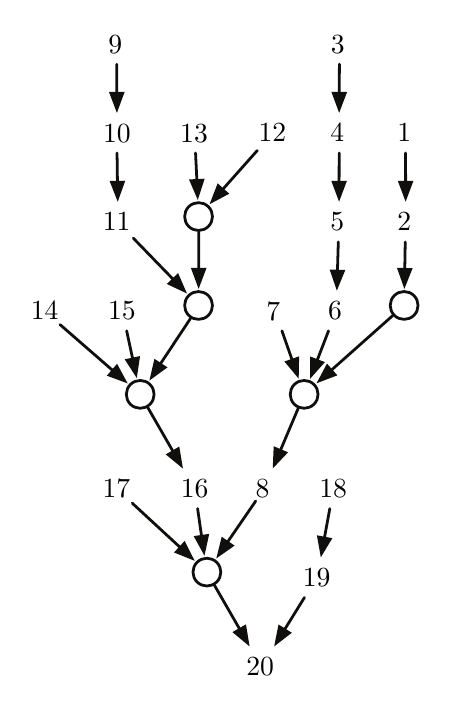
\begin{tikzpicture}
\pgfpathmoveto{\pgfqpoint{0cm}{-0.071cm}}
\pgfpathlineto{\pgfqpoint{5.009cm}{-0.071cm}}
\pgfpathlineto{\pgfqpoint{5.009cm}{8.361cm}}
\pgfpathlineto{\pgfqpoint{0cm}{8.361cm}}
\pgfpathclose
\pgfusepath{clip}
\definecolor{eps2pgf_color}{gray}{0}\pgfsetstrokecolor{eps2pgf_color}\pgfsetfillcolor{eps2pgf_color}
\pgftext[x=2.952cm,y=0.247cm,rotate=0]{20}
\pgftext[x=3.879cm,y=2.505cm,rotate=0]{18}
\pgftext[x=1.128cm,y=2.506cm,rotate=0]{17}
\pgftext[x=2.12cm,y=2.506cm,rotate=0]{16}
\pgftext[x=0.216cm,y=4.765cm,rotate=0]{14}
\pgftext[x=1.197cm,y=4.765cm,rotate=0]{15}
\pgftext[x=2.113cm,y=7.02cm,rotate=0]{13}
\pgftext[x=3.109cm,y=7.023cm,rotate=0]{12}
\pgftext[x=1.043cm,y=5.894cm,rotate=0]{1}
\pgftext[x=1.216cm,y=5.894cm,rotate=0]{1}
\pgftext[x=1.134cm,y=7.02cm,rotate=0]{10}
\pgftext[x=1.112cm,y=8.148cm,rotate=0]{9}
\pgftext[x=2.984cm,y=2.505cm,rotate=0]{8}
\pgftext[x=3.119cm,y=4.761cm,rotate=0]{7}
\pgftext[x=3.902cm,y=4.764cm,rotate=0]{6}
\pgftext[x=3.931cm,y=5.894cm,rotate=0]{5}
\pgftext[x=3.933cm,y=7.023cm,rotate=0]{4}
\pgftext[x=3.94cm,y=8.149cm,rotate=0]{3}
\pgftext[x=4.784cm,y=5.894cm,rotate=0]{2}
\pgftext[x=4.784cm,y=7.023cm,rotate=0]{1}
\pgfsetdash{}{0cm}
\pgfsetlinewidth{0.353mm}
\pgfsetroundcap
\pgfsetroundjoin
\definecolor{eps2pgf_color}{cmyk}{0.75021,0.679683,0.670222,0.90164}\pgfsetstrokecolor{eps2pgf_color}\pgfsetfillcolor{eps2pgf_color}
\pgfpathmoveto{\pgfqpoint{2.401cm}{1.571cm}}
\pgfpathcurveto{\pgfqpoint{2.47cm}{1.502cm}}{\pgfqpoint{2.47cm}{1.39cm}}{\pgfqpoint{2.401cm}{1.322cm}}
\pgfpathcurveto{\pgfqpoint{2.332cm}{1.253cm}}{\pgfqpoint{2.22cm}{1.253cm}}{\pgfqpoint{2.151cm}{1.322cm}}
\pgfpathcurveto{\pgfqpoint{2.082cm}{1.39cm}}{\pgfqpoint{2.082cm}{1.502cm}}{\pgfqpoint{2.151cm}{1.571cm}}
\pgfpathcurveto{\pgfqpoint{2.22cm}{1.64cm}}{\pgfqpoint{2.332cm}{1.64cm}}{\pgfqpoint{2.401cm}{1.571cm}}
\pgfusepath{stroke}
\pgfsetdash{}{0cm}
\pgfpathmoveto{\pgfqpoint{2.695cm}{0.718cm}}
\pgfpathlineto{\pgfqpoint{2.373cm}{1.278cm}}
\pgfusepath{stroke}
\pgfpathmoveto{\pgfqpoint{2.793cm}{0.547cm}}
\pgfpathlineto{\pgfqpoint{2.759cm}{0.755cm}}
\pgfpathlineto{\pgfqpoint{2.631cm}{0.682cm}}
\pgfpathlineto{\pgfqpoint{2.793cm}{0.547cm}}
\pgfpathclose
\pgfusepath{fill}
\pgfsetdash{}{0cm}
\pgfsetbuttcap
\pgfsetmiterjoin
\pgfpathmoveto{\pgfqpoint{2.793cm}{0.547cm}}
\pgfpathlineto{\pgfqpoint{2.759cm}{0.755cm}}
\pgfpathlineto{\pgfqpoint{2.631cm}{0.682cm}}
\pgfpathlineto{\pgfqpoint{2.793cm}{0.547cm}}
\pgfpathclose
\pgfusepath{stroke}
\definecolor{eps2pgf_color}{gray}{0}\pgfsetstrokecolor{eps2pgf_color}\pgfsetfillcolor{eps2pgf_color}
\pgftext[x=3.67cm,y=1.374cm,rotate=0]{19}
\pgfsetdash{}{0cm}
\pgfsetroundcap
\pgfsetroundjoin
\definecolor{eps2pgf_color}{cmyk}{0.75021,0.679683,0.670222,0.90164}\pgfsetstrokecolor{eps2pgf_color}\pgfsetfillcolor{eps2pgf_color}
\pgfpathmoveto{\pgfqpoint{3.261cm}{0.714cm}}
\pgfpathlineto{\pgfqpoint{3.515cm}{1.124cm}}
\pgfusepath{stroke}
\pgfpathmoveto{\pgfqpoint{3.157cm}{0.546cm}}
\pgfpathlineto{\pgfqpoint{3.324cm}{0.675cm}}
\pgfpathlineto{\pgfqpoint{3.198cm}{0.753cm}}
\pgfpathlineto{\pgfqpoint{3.157cm}{0.546cm}}
\pgfpathclose
\pgfusepath{fill}
\pgfsetdash{}{0cm}
\pgfsetbuttcap
\pgfsetmiterjoin
\pgfpathmoveto{\pgfqpoint{3.157cm}{0.546cm}}
\pgfpathlineto{\pgfqpoint{3.324cm}{0.675cm}}
\pgfpathlineto{\pgfqpoint{3.198cm}{0.753cm}}
\pgfpathlineto{\pgfqpoint{3.157cm}{0.546cm}}
\pgfpathclose
\pgfusepath{stroke}
\pgfsetdash{}{0cm}
\pgfsetroundcap
\pgfsetroundjoin
\pgfpathmoveto{\pgfqpoint{3.768cm}{1.878cm}}
\pgfpathlineto{\pgfqpoint{3.837cm}{2.253cm}}
\pgfusepath{stroke}
\pgfpathmoveto{\pgfqpoint{3.732cm}{1.684cm}}
\pgfpathlineto{\pgfqpoint{3.841cm}{1.865cm}}
\pgfpathlineto{\pgfqpoint{3.695cm}{1.892cm}}
\pgfpathlineto{\pgfqpoint{3.732cm}{1.684cm}}
\pgfpathclose
\pgfusepath{fill}
\pgfsetdash{}{0cm}
\pgfsetbuttcap
\pgfsetmiterjoin
\pgfpathmoveto{\pgfqpoint{3.732cm}{1.684cm}}
\pgfpathlineto{\pgfqpoint{3.841cm}{1.865cm}}
\pgfpathlineto{\pgfqpoint{3.695cm}{1.892cm}}
\pgfpathlineto{\pgfqpoint{3.732cm}{1.684cm}}
\pgfpathclose
\pgfusepath{stroke}
\pgfsetdash{}{0cm}
\pgfsetroundcap
\pgfsetroundjoin
\pgfpathmoveto{\pgfqpoint{1.939cm}{1.758cm}}
\pgfpathlineto{\pgfqpoint{1.328cm}{2.322cm}}
\pgfusepath{stroke}
\pgfpathmoveto{\pgfqpoint{2.084cm}{1.624cm}}
\pgfpathlineto{\pgfqpoint{1.989cm}{1.812cm}}
\pgfpathlineto{\pgfqpoint{1.889cm}{1.703cm}}
\pgfpathlineto{\pgfqpoint{2.084cm}{1.624cm}}
\pgfpathclose
\pgfusepath{fill}
\pgfsetdash{}{0cm}
\pgfsetbuttcap
\pgfsetmiterjoin
\pgfpathmoveto{\pgfqpoint{2.084cm}{1.624cm}}
\pgfpathlineto{\pgfqpoint{1.989cm}{1.812cm}}
\pgfpathlineto{\pgfqpoint{1.889cm}{1.703cm}}
\pgfpathlineto{\pgfqpoint{2.084cm}{1.624cm}}
\pgfpathclose
\pgfusepath{stroke}
\pgfsetdash{}{0cm}
\pgfsetroundcap
\pgfsetroundjoin
\pgfpathmoveto{\pgfqpoint{2.209cm}{1.9cm}}
\pgfpathlineto{\pgfqpoint{2.158cm}{2.253cm}}
\pgfusepath{stroke}
\pgfpathmoveto{\pgfqpoint{2.238cm}{1.705cm}}
\pgfpathlineto{\pgfqpoint{2.283cm}{1.911cm}}
\pgfpathlineto{\pgfqpoint{2.136cm}{1.89cm}}
\pgfpathlineto{\pgfqpoint{2.238cm}{1.705cm}}
\pgfpathclose
\pgfusepath{fill}
\pgfsetdash{}{0cm}
\pgfsetbuttcap
\pgfsetmiterjoin
\pgfpathmoveto{\pgfqpoint{2.238cm}{1.705cm}}
\pgfpathlineto{\pgfqpoint{2.283cm}{1.911cm}}
\pgfpathlineto{\pgfqpoint{2.136cm}{1.89cm}}
\pgfpathlineto{\pgfqpoint{2.238cm}{1.705cm}}
\pgfpathclose
\pgfusepath{stroke}
\pgfsetdash{}{0cm}
\pgfsetroundcap
\pgfsetroundjoin
\pgfpathmoveto{\pgfqpoint{1.554cm}{3.829cm}}
\pgfpathcurveto{\pgfqpoint{1.623cm}{3.76cm}}{\pgfqpoint{1.623cm}{3.648cm}}{\pgfqpoint{1.554cm}{3.579cm}}
\pgfpathcurveto{\pgfqpoint{1.485cm}{3.51cm}}{\pgfqpoint{1.373cm}{3.51cm}}{\pgfqpoint{1.304cm}{3.579cm}}
\pgfpathcurveto{\pgfqpoint{1.236cm}{3.648cm}}{\pgfqpoint{1.236cm}{3.76cm}}{\pgfqpoint{1.304cm}{3.829cm}}
\pgfpathcurveto{\pgfqpoint{1.373cm}{3.898cm}}{\pgfqpoint{1.485cm}{3.898cm}}{\pgfqpoint{1.554cm}{3.829cm}}
\pgfusepath{stroke}
\pgfsetdash{}{0cm}
\pgfpathmoveto{\pgfqpoint{1.848cm}{2.976cm}}
\pgfpathlineto{\pgfqpoint{1.526cm}{3.536cm}}
\pgfusepath{stroke}
\pgfpathmoveto{\pgfqpoint{1.947cm}{2.805cm}}
\pgfpathlineto{\pgfqpoint{1.912cm}{3.013cm}}
\pgfpathlineto{\pgfqpoint{1.784cm}{2.939cm}}
\pgfpathlineto{\pgfqpoint{1.947cm}{2.805cm}}
\pgfpathclose
\pgfusepath{fill}
\pgfsetdash{}{0cm}
\pgfsetbuttcap
\pgfsetmiterjoin
\pgfpathmoveto{\pgfqpoint{1.947cm}{2.805cm}}
\pgfpathlineto{\pgfqpoint{1.912cm}{3.013cm}}
\pgfpathlineto{\pgfqpoint{1.784cm}{2.939cm}}
\pgfpathlineto{\pgfqpoint{1.947cm}{2.805cm}}
\pgfpathclose
\pgfusepath{stroke}
\pgfsetdash{}{0cm}
\pgfsetroundcap
\pgfsetroundjoin
\pgfpathmoveto{\pgfqpoint{1.083cm}{4.005cm}}
\pgfpathlineto{\pgfqpoint{0.411cm}{4.59cm}}
\pgfusepath{stroke}
\pgfpathmoveto{\pgfqpoint{1.232cm}{3.876cm}}
\pgfpathlineto{\pgfqpoint{1.132cm}{4.061cm}}
\pgfpathlineto{\pgfqpoint{1.035cm}{3.949cm}}
\pgfpathlineto{\pgfqpoint{1.232cm}{3.876cm}}
\pgfpathclose
\pgfusepath{fill}
\pgfsetdash{}{0cm}
\pgfsetbuttcap
\pgfsetmiterjoin
\pgfpathmoveto{\pgfqpoint{1.232cm}{3.876cm}}
\pgfpathlineto{\pgfqpoint{1.132cm}{4.061cm}}
\pgfpathlineto{\pgfqpoint{1.035cm}{3.949cm}}
\pgfpathlineto{\pgfqpoint{1.232cm}{3.876cm}}
\pgfpathclose
\pgfusepath{stroke}
\pgfsetdash{}{0cm}
\pgfsetroundcap
\pgfsetroundjoin
\pgfpathmoveto{\pgfqpoint{2.295cm}{4.958cm}}
\pgfpathcurveto{\pgfqpoint{2.364cm}{4.889cm}}{\pgfqpoint{2.364cm}{4.777cm}}{\pgfqpoint{2.295cm}{4.708cm}}
\pgfpathcurveto{\pgfqpoint{2.226cm}{4.639cm}}{\pgfqpoint{2.114cm}{4.639cm}}{\pgfqpoint{2.045cm}{4.708cm}}
\pgfpathcurveto{\pgfqpoint{1.976cm}{4.777cm}}{\pgfqpoint{1.976cm}{4.889cm}}{\pgfqpoint{2.045cm}{4.958cm}}
\pgfpathcurveto{\pgfqpoint{2.114cm}{5.027cm}}{\pgfqpoint{2.226cm}{5.027cm}}{\pgfqpoint{2.295cm}{4.958cm}}
\pgfusepath{stroke}
\pgfsetdash{}{0cm}
\pgfpathmoveto{\pgfqpoint{1.683cm}{4.087cm}}
\pgfpathlineto{\pgfqpoint{2.068cm}{4.668cm}}
\pgfusepath{stroke}
\pgfpathmoveto{\pgfqpoint{1.574cm}{3.922cm}}
\pgfpathlineto{\pgfqpoint{1.745cm}{4.046cm}}
\pgfpathlineto{\pgfqpoint{1.621cm}{4.127cm}}
\pgfpathlineto{\pgfqpoint{1.574cm}{3.922cm}}
\pgfpathclose
\pgfusepath{fill}
\pgfsetdash{}{0cm}
\pgfsetbuttcap
\pgfsetmiterjoin
\pgfpathmoveto{\pgfqpoint{1.574cm}{3.922cm}}
\pgfpathlineto{\pgfqpoint{1.745cm}{4.046cm}}
\pgfpathlineto{\pgfqpoint{1.621cm}{4.127cm}}
\pgfpathlineto{\pgfqpoint{1.574cm}{3.922cm}}
\pgfpathclose
\pgfusepath{stroke}
\pgfsetdash{}{0cm}
\pgfsetroundcap
\pgfsetroundjoin
\pgfpathmoveto{\pgfqpoint{1.851cm}{5.162cm}}
\pgfpathlineto{\pgfqpoint{1.341cm}{5.688cm}}
\pgfusepath{stroke}
\pgfpathmoveto{\pgfqpoint{1.988cm}{5.021cm}}
\pgfpathlineto{\pgfqpoint{1.904cm}{5.214cm}}
\pgfpathlineto{\pgfqpoint{1.797cm}{5.111cm}}
\pgfpathlineto{\pgfqpoint{1.988cm}{5.021cm}}
\pgfpathclose
\pgfusepath{fill}
\pgfsetdash{}{0cm}
\pgfsetbuttcap
\pgfsetmiterjoin
\pgfpathmoveto{\pgfqpoint{1.988cm}{5.021cm}}
\pgfpathlineto{\pgfqpoint{1.904cm}{5.214cm}}
\pgfpathlineto{\pgfqpoint{1.797cm}{5.111cm}}
\pgfpathlineto{\pgfqpoint{1.988cm}{5.021cm}}
\pgfpathclose
\pgfusepath{stroke}
\pgfsetdash{}{0cm}
\pgfsetroundcap
\pgfsetroundjoin
\pgfpathmoveto{\pgfqpoint{1.14cm}{6.398cm}}
\pgfpathlineto{\pgfqpoint{1.135cm}{6.769cm}}
\pgfusepath{stroke}
\pgfpathmoveto{\pgfqpoint{1.143cm}{6.201cm}}
\pgfpathlineto{\pgfqpoint{1.214cm}{6.399cm}}
\pgfpathlineto{\pgfqpoint{1.066cm}{6.397cm}}
\pgfpathlineto{\pgfqpoint{1.143cm}{6.201cm}}
\pgfpathclose
\pgfusepath{fill}
\pgfsetdash{}{0cm}
\pgfsetbuttcap
\pgfsetmiterjoin
\pgfpathmoveto{\pgfqpoint{1.143cm}{6.201cm}}
\pgfpathlineto{\pgfqpoint{1.214cm}{6.399cm}}
\pgfpathlineto{\pgfqpoint{1.066cm}{6.397cm}}
\pgfpathlineto{\pgfqpoint{1.143cm}{6.201cm}}
\pgfpathclose
\pgfusepath{stroke}
\pgfsetdash{}{0cm}
\pgfsetroundcap
\pgfsetroundjoin
\pgfpathmoveto{\pgfqpoint{2.295cm}{6.087cm}}
\pgfpathcurveto{\pgfqpoint{2.364cm}{6.018cm}}{\pgfqpoint{2.364cm}{5.906cm}}{\pgfqpoint{2.295cm}{5.837cm}}
\pgfpathcurveto{\pgfqpoint{2.226cm}{5.768cm}}{\pgfqpoint{2.114cm}{5.768cm}}{\pgfqpoint{2.045cm}{5.837cm}}
\pgfpathcurveto{\pgfqpoint{1.976cm}{5.906cm}}{\pgfqpoint{1.976cm}{6.018cm}}{\pgfqpoint{2.045cm}{6.087cm}}
\pgfpathcurveto{\pgfqpoint{2.114cm}{6.156cm}}{\pgfqpoint{2.226cm}{6.156cm}}{\pgfqpoint{2.295cm}{6.087cm}}
\pgfusepath{stroke}
\pgfsetdash{}{0cm}
\pgfpathmoveto{\pgfqpoint{2.172cm}{5.292cm}}
\pgfpathlineto{\pgfqpoint{2.174cm}{5.768cm}}
\pgfusepath{stroke}
\pgfpathmoveto{\pgfqpoint{2.171cm}{5.094cm}}
\pgfpathlineto{\pgfqpoint{2.246cm}{5.292cm}}
\pgfpathlineto{\pgfqpoint{2.098cm}{5.292cm}}
\pgfpathlineto{\pgfqpoint{2.171cm}{5.094cm}}
\pgfpathclose
\pgfusepath{fill}
\pgfsetdash{}{0cm}
\pgfsetbuttcap
\pgfsetmiterjoin
\pgfpathmoveto{\pgfqpoint{2.171cm}{5.094cm}}
\pgfpathlineto{\pgfqpoint{2.246cm}{5.292cm}}
\pgfpathlineto{\pgfqpoint{2.098cm}{5.292cm}}
\pgfpathlineto{\pgfqpoint{2.171cm}{5.094cm}}
\pgfpathclose
\pgfusepath{stroke}
\pgfsetdash{}{0cm}
\pgfsetroundcap
\pgfsetroundjoin
\pgfpathmoveto{\pgfqpoint{2.149cm}{6.42cm}}
\pgfpathlineto{\pgfqpoint{2.132cm}{6.769cm}}
\pgfusepath{stroke}
\pgfpathmoveto{\pgfqpoint{2.158cm}{6.223cm}}
\pgfpathlineto{\pgfqpoint{2.223cm}{6.424cm}}
\pgfpathlineto{\pgfqpoint{2.075cm}{6.417cm}}
\pgfpathlineto{\pgfqpoint{2.158cm}{6.223cm}}
\pgfpathclose
\pgfusepath{fill}
\pgfsetdash{}{0cm}
\pgfsetbuttcap
\pgfsetmiterjoin
\pgfpathmoveto{\pgfqpoint{2.158cm}{6.223cm}}
\pgfpathlineto{\pgfqpoint{2.223cm}{6.424cm}}
\pgfpathlineto{\pgfqpoint{2.075cm}{6.417cm}}
\pgfpathlineto{\pgfqpoint{2.158cm}{6.223cm}}
\pgfpathclose
\pgfusepath{stroke}
\pgfsetdash{}{0cm}
\pgfsetroundcap
\pgfsetroundjoin
\pgfpathmoveto{\pgfqpoint{2.475cm}{6.305cm}}
\pgfpathlineto{\pgfqpoint{2.916cm}{6.801cm}}
\pgfusepath{stroke}
\pgfpathmoveto{\pgfqpoint{2.344cm}{6.157cm}}
\pgfpathlineto{\pgfqpoint{2.53cm}{6.256cm}}
\pgfpathlineto{\pgfqpoint{2.42cm}{6.354cm}}
\pgfpathlineto{\pgfqpoint{2.344cm}{6.157cm}}
\pgfpathclose
\pgfusepath{fill}
\pgfsetdash{}{0cm}
\pgfsetbuttcap
\pgfsetmiterjoin
\pgfpathmoveto{\pgfqpoint{2.344cm}{6.157cm}}
\pgfpathlineto{\pgfqpoint{2.53cm}{6.256cm}}
\pgfpathlineto{\pgfqpoint{2.42cm}{6.354cm}}
\pgfpathlineto{\pgfqpoint{2.344cm}{6.157cm}}
\pgfpathclose
\pgfusepath{stroke}
\pgfsetdash{}{0cm}
\pgfsetroundcap
\pgfsetroundjoin
\pgfpathmoveto{\pgfqpoint{1.334cm}{4.153cm}}
\pgfpathlineto{\pgfqpoint{1.257cm}{4.511cm}}
\pgfusepath{stroke}
\pgfpathmoveto{\pgfqpoint{1.375cm}{3.96cm}}
\pgfpathlineto{\pgfqpoint{1.406cm}{4.168cm}}
\pgfpathlineto{\pgfqpoint{1.261cm}{4.137cm}}
\pgfpathlineto{\pgfqpoint{1.375cm}{3.96cm}}
\pgfpathclose
\pgfusepath{fill}
\pgfsetdash{}{0cm}
\pgfsetbuttcap
\pgfsetmiterjoin
\pgfpathmoveto{\pgfqpoint{1.375cm}{3.96cm}}
\pgfpathlineto{\pgfqpoint{1.406cm}{4.168cm}}
\pgfpathlineto{\pgfqpoint{1.261cm}{4.137cm}}
\pgfpathlineto{\pgfqpoint{1.375cm}{3.96cm}}
\pgfpathclose
\pgfusepath{stroke}
\pgfsetdash{}{0cm}
\pgfsetroundcap
\pgfsetroundjoin
\pgfpathmoveto{\pgfqpoint{2.536cm}{1.825cm}}
\pgfpathlineto{\pgfqpoint{2.896cm}{2.349cm}}
\pgfusepath{stroke}
\pgfpathmoveto{\pgfqpoint{2.424cm}{1.662cm}}
\pgfpathlineto{\pgfqpoint{2.597cm}{1.783cm}}
\pgfpathlineto{\pgfqpoint{2.475cm}{1.867cm}}
\pgfpathlineto{\pgfqpoint{2.424cm}{1.662cm}}
\pgfpathclose
\pgfusepath{fill}
\pgfsetdash{}{0cm}
\pgfsetbuttcap
\pgfsetmiterjoin
\pgfpathmoveto{\pgfqpoint{2.424cm}{1.662cm}}
\pgfpathlineto{\pgfqpoint{2.597cm}{1.783cm}}
\pgfpathlineto{\pgfqpoint{2.475cm}{1.867cm}}
\pgfpathlineto{\pgfqpoint{2.424cm}{1.662cm}}
\pgfpathclose
\pgfusepath{stroke}
\pgfsetdash{}{0cm}
\pgfsetroundcap
\pgfsetroundjoin
\pgfpathmoveto{\pgfqpoint{4.906cm}{4.958cm}}
\pgfpathcurveto{\pgfqpoint{4.975cm}{4.889cm}}{\pgfqpoint{4.975cm}{4.777cm}}{\pgfqpoint{4.906cm}{4.708cm}}
\pgfpathcurveto{\pgfqpoint{4.837cm}{4.639cm}}{\pgfqpoint{4.725cm}{4.639cm}}{\pgfqpoint{4.656cm}{4.708cm}}
\pgfpathcurveto{\pgfqpoint{4.587cm}{4.777cm}}{\pgfqpoint{4.587cm}{4.889cm}}{\pgfqpoint{4.656cm}{4.958cm}}
\pgfpathcurveto{\pgfqpoint{4.725cm}{5.027cm}}{\pgfqpoint{4.837cm}{5.027cm}}{\pgfqpoint{4.906cm}{4.958cm}}
\pgfusepath{stroke}
\pgfsetdash{}{0cm}
\pgfpathmoveto{\pgfqpoint{3.636cm}{3.829cm}}
\pgfpathcurveto{\pgfqpoint{3.705cm}{3.76cm}}{\pgfqpoint{3.705cm}{3.648cm}}{\pgfqpoint{3.636cm}{3.579cm}}
\pgfpathcurveto{\pgfqpoint{3.567cm}{3.51cm}}{\pgfqpoint{3.455cm}{3.51cm}}{\pgfqpoint{3.386cm}{3.579cm}}
\pgfpathcurveto{\pgfqpoint{3.317cm}{3.648cm}}{\pgfqpoint{3.317cm}{3.76cm}}{\pgfqpoint{3.386cm}{3.829cm}}
\pgfpathcurveto{\pgfqpoint{3.455cm}{3.898cm}}{\pgfqpoint{3.567cm}{3.898cm}}{\pgfqpoint{3.636cm}{3.829cm}}
\pgfusepath{stroke}
\pgfsetdash{}{0cm}
\pgfpathmoveto{\pgfqpoint{3.209cm}{2.991cm}}
\pgfpathlineto{\pgfqpoint{3.435cm}{3.525cm}}
\pgfusepath{stroke}
\pgfpathmoveto{\pgfqpoint{3.132cm}{2.809cm}}
\pgfpathlineto{\pgfqpoint{3.277cm}{2.962cm}}
\pgfpathlineto{\pgfqpoint{3.141cm}{3.019cm}}
\pgfpathlineto{\pgfqpoint{3.132cm}{2.809cm}}
\pgfpathclose
\pgfusepath{fill}
\pgfsetdash{}{0cm}
\pgfsetbuttcap
\pgfsetmiterjoin
\pgfpathmoveto{\pgfqpoint{3.132cm}{2.809cm}}
\pgfpathlineto{\pgfqpoint{3.277cm}{2.962cm}}
\pgfpathlineto{\pgfqpoint{3.141cm}{3.019cm}}
\pgfpathlineto{\pgfqpoint{3.132cm}{2.809cm}}
\pgfpathclose
\pgfusepath{stroke}
\pgfsetdash{}{0cm}
\pgfsetroundcap
\pgfsetroundjoin
\pgfpathmoveto{\pgfqpoint{3.854cm}{4.009cm}}
\pgfpathlineto{\pgfqpoint{4.636cm}{4.704cm}}
\pgfusepath{stroke}
\pgfpathmoveto{\pgfqpoint{3.706cm}{3.878cm}}
\pgfpathlineto{\pgfqpoint{3.903cm}{3.953cm}}
\pgfpathlineto{\pgfqpoint{3.805cm}{4.064cm}}
\pgfpathlineto{\pgfqpoint{3.706cm}{3.878cm}}
\pgfpathclose
\pgfusepath{fill}
\pgfsetdash{}{0cm}
\pgfsetbuttcap
\pgfsetmiterjoin
\pgfpathmoveto{\pgfqpoint{3.706cm}{3.878cm}}
\pgfpathlineto{\pgfqpoint{3.903cm}{3.953cm}}
\pgfpathlineto{\pgfqpoint{3.805cm}{4.064cm}}
\pgfpathlineto{\pgfqpoint{3.706cm}{3.878cm}}
\pgfpathclose
\pgfusepath{stroke}
\pgfsetdash{}{0cm}
\pgfsetroundcap
\pgfsetroundjoin
\pgfpathmoveto{\pgfqpoint{3.675cm}{4.132cm}}
\pgfpathlineto{\pgfqpoint{3.821cm}{4.511cm}}
\pgfusepath{stroke}
\pgfpathmoveto{\pgfqpoint{3.604cm}{3.948cm}}
\pgfpathlineto{\pgfqpoint{3.745cm}{4.106cm}}
\pgfpathlineto{\pgfqpoint{3.606cm}{4.159cm}}
\pgfpathlineto{\pgfqpoint{3.604cm}{3.948cm}}
\pgfpathclose
\pgfusepath{fill}
\pgfsetdash{}{0cm}
\pgfsetbuttcap
\pgfsetmiterjoin
\pgfpathmoveto{\pgfqpoint{3.604cm}{3.948cm}}
\pgfpathlineto{\pgfqpoint{3.745cm}{4.106cm}}
\pgfpathlineto{\pgfqpoint{3.606cm}{4.159cm}}
\pgfpathlineto{\pgfqpoint{3.604cm}{3.948cm}}
\pgfpathclose
\pgfusepath{stroke}
\pgfsetdash{}{0cm}
\pgfsetroundcap
\pgfsetroundjoin
\pgfpathmoveto{\pgfqpoint{4.789cm}{5.292cm}}
\pgfpathlineto{\pgfqpoint{4.795cm}{5.64cm}}
\pgfusepath{stroke}
\pgfpathmoveto{\pgfqpoint{4.785cm}{5.094cm}}
\pgfpathlineto{\pgfqpoint{4.863cm}{5.29cm}}
\pgfpathlineto{\pgfqpoint{4.715cm}{5.293cm}}
\pgfpathlineto{\pgfqpoint{4.785cm}{5.094cm}}
\pgfpathclose
\pgfusepath{fill}
\pgfsetdash{}{0cm}
\pgfsetbuttcap
\pgfsetmiterjoin
\pgfpathmoveto{\pgfqpoint{4.785cm}{5.094cm}}
\pgfpathlineto{\pgfqpoint{4.863cm}{5.29cm}}
\pgfpathlineto{\pgfqpoint{4.715cm}{5.293cm}}
\pgfpathlineto{\pgfqpoint{4.785cm}{5.094cm}}
\pgfpathclose
\pgfusepath{stroke}
\pgfsetdash{}{0cm}
\pgfsetroundcap
\pgfsetroundjoin
\pgfpathmoveto{\pgfqpoint{4.8cm}{6.398cm}}
\pgfpathlineto{\pgfqpoint{4.799cm}{6.769cm}}
\pgfusepath{stroke}
\pgfpathmoveto{\pgfqpoint{4.8cm}{6.201cm}}
\pgfpathlineto{\pgfqpoint{4.874cm}{6.398cm}}
\pgfpathlineto{\pgfqpoint{4.726cm}{6.398cm}}
\pgfpathlineto{\pgfqpoint{4.8cm}{6.201cm}}
\pgfpathclose
\pgfusepath{fill}
\pgfsetdash{}{0cm}
\pgfsetbuttcap
\pgfsetmiterjoin
\pgfpathmoveto{\pgfqpoint{4.8cm}{6.201cm}}
\pgfpathlineto{\pgfqpoint{4.874cm}{6.398cm}}
\pgfpathlineto{\pgfqpoint{4.726cm}{6.398cm}}
\pgfpathlineto{\pgfqpoint{4.8cm}{6.201cm}}
\pgfpathclose
\pgfusepath{stroke}
\pgfsetdash{}{0cm}
\pgfsetroundcap
\pgfsetroundjoin
\pgfpathmoveto{\pgfqpoint{3.934cm}{5.269cm}}
\pgfpathlineto{\pgfqpoint{3.945cm}{5.64cm}}
\pgfusepath{stroke}
\pgfpathmoveto{\pgfqpoint{3.928cm}{5.072cm}}
\pgfpathlineto{\pgfqpoint{4.008cm}{5.267cm}}
\pgfpathlineto{\pgfqpoint{3.86cm}{5.271cm}}
\pgfpathlineto{\pgfqpoint{3.928cm}{5.072cm}}
\pgfpathclose
\pgfusepath{fill}
\pgfsetdash{}{0cm}
\pgfsetbuttcap
\pgfsetmiterjoin
\pgfpathmoveto{\pgfqpoint{3.928cm}{5.072cm}}
\pgfpathlineto{\pgfqpoint{4.008cm}{5.267cm}}
\pgfpathlineto{\pgfqpoint{3.86cm}{5.271cm}}
\pgfpathlineto{\pgfqpoint{3.928cm}{5.072cm}}
\pgfpathclose
\pgfusepath{stroke}
\pgfsetdash{}{0cm}
\pgfsetroundcap
\pgfsetroundjoin
\pgfpathmoveto{\pgfqpoint{3.955cm}{6.398cm}}
\pgfpathlineto{\pgfqpoint{3.956cm}{6.769cm}}
\pgfusepath{stroke}
\pgfpathmoveto{\pgfqpoint{3.955cm}{6.201cm}}
\pgfpathlineto{\pgfqpoint{4.029cm}{6.398cm}}
\pgfpathlineto{\pgfqpoint{3.881cm}{6.398cm}}
\pgfpathlineto{\pgfqpoint{3.955cm}{6.201cm}}
\pgfpathclose
\pgfusepath{fill}
\pgfsetdash{}{0cm}
\pgfsetbuttcap
\pgfsetmiterjoin
\pgfpathmoveto{\pgfqpoint{3.955cm}{6.201cm}}
\pgfpathlineto{\pgfqpoint{4.029cm}{6.398cm}}
\pgfpathlineto{\pgfqpoint{3.881cm}{6.398cm}}
\pgfpathlineto{\pgfqpoint{3.955cm}{6.201cm}}
\pgfpathclose
\pgfusepath{stroke}
\pgfsetdash{}{0cm}
\pgfsetroundcap
\pgfsetroundjoin
\pgfpathmoveto{\pgfqpoint{1.132cm}{7.527cm}}
\pgfpathlineto{\pgfqpoint{1.131cm}{7.897cm}}
\pgfusepath{stroke}
\pgfpathmoveto{\pgfqpoint{1.133cm}{7.329cm}}
\pgfpathlineto{\pgfqpoint{1.206cm}{7.527cm}}
\pgfpathlineto{\pgfqpoint{1.058cm}{7.527cm}}
\pgfpathlineto{\pgfqpoint{1.133cm}{7.329cm}}
\pgfpathclose
\pgfusepath{fill}
\pgfsetdash{}{0cm}
\pgfsetbuttcap
\pgfsetmiterjoin
\pgfpathmoveto{\pgfqpoint{1.133cm}{7.329cm}}
\pgfpathlineto{\pgfqpoint{1.206cm}{7.527cm}}
\pgfpathlineto{\pgfqpoint{1.058cm}{7.527cm}}
\pgfpathlineto{\pgfqpoint{1.133cm}{7.329cm}}
\pgfpathclose
\pgfusepath{stroke}
\pgfsetdash{}{0cm}
\pgfsetroundcap
\pgfsetroundjoin
\pgfpathmoveto{\pgfqpoint{3.957cm}{7.527cm}}
\pgfpathlineto{\pgfqpoint{3.959cm}{7.897cm}}
\pgfusepath{stroke}
\pgfpathmoveto{\pgfqpoint{3.956cm}{7.329cm}}
\pgfpathlineto{\pgfqpoint{4.031cm}{7.527cm}}
\pgfpathlineto{\pgfqpoint{3.883cm}{7.527cm}}
\pgfpathlineto{\pgfqpoint{3.956cm}{7.329cm}}
\pgfpathclose
\pgfusepath{fill}
\pgfsetdash{}{0cm}
\pgfsetbuttcap
\pgfsetmiterjoin
\pgfpathmoveto{\pgfqpoint{3.956cm}{7.329cm}}
\pgfpathlineto{\pgfqpoint{4.031cm}{7.527cm}}
\pgfpathlineto{\pgfqpoint{3.883cm}{7.527cm}}
\pgfpathlineto{\pgfqpoint{3.956cm}{7.329cm}}
\pgfpathclose
\pgfusepath{stroke}
\pgfsetdash{}{0cm}
\pgfsetroundcap
\pgfsetroundjoin
\pgfpathmoveto{\pgfqpoint{3.36cm}{4.137cm}}
\pgfpathlineto{\pgfqpoint{3.229cm}{4.511cm}}
\pgfusepath{stroke}
\pgfpathmoveto{\pgfqpoint{3.425cm}{3.951cm}}
\pgfpathlineto{\pgfqpoint{3.429cm}{4.162cm}}
\pgfpathlineto{\pgfqpoint{3.29cm}{4.113cm}}
\pgfpathlineto{\pgfqpoint{3.425cm}{3.951cm}}
\pgfpathclose
\pgfusepath{fill}
\pgfsetdash{}{0cm}
\pgfsetbuttcap
\pgfsetmiterjoin
\pgfpathmoveto{\pgfqpoint{3.425cm}{3.951cm}}
\pgfpathlineto{\pgfqpoint{3.429cm}{4.162cm}}
\pgfpathlineto{\pgfqpoint{3.29cm}{4.113cm}}
\pgfpathlineto{\pgfqpoint{3.425cm}{3.951cm}}
\pgfpathclose
\pgfusepath{stroke}
\begin{pgfscope}
\end{pgfscope}
\end{tikzpicture}

   %\includegraphics[width=.8\textwidth]{map_both.pdf} 
   \caption{Map of UCRB with site numbers.}
   \label{fig:map}
\end{figure}

% latex table generated in R 2.12.0 by xtable 1.5-6 package
% Fri Jan  7 16:43:47 2011
\begin{table}[ht]
\begin{center}
\begin{tabular}{rrp{5cm}}
  \toprule
 Node & USGS Gauge & Site Name \\ 
  \midrule
  1  & 09072500 &  Colorado River At Glenwood Springs, CO        \\ 
  2  & 09095500 &  Colorado River Near Cameo, CO                 \\ 
  3  & 09109000 &  Taylor River Below Taylor Park Reservoir, CO  \\ 
  4  & 09124700 &  Gunnision River Above Blue Mesa Reservoir, CO \\ 
  5  & 09127800 &  Gunnison River At Crystal Reservoir, CO       \\ 
  6  & 09152500 &  Gunnison River Near Grand Junction, CO        \\ 
  7  & 09180000 &  Dolores River Near Cisco, UT                  \\ 
  8  & 09180500 &  Colorado River Near Cisco, UT                 \\ 
  9  & 09211200 &  Green R Bel Fontenelle Res, WY                \\ 
  10 & 09217000 &  Green R. Nr Green River, WY                   \\ 
  11 & 09234500 &  Green River Near Greendale, UT                \\ 
  12 & 09251000 &  Yampa River Near Maybell, CO                  \\ 
  13 & 09260000 &  Little Snake River Near Lily, CO              \\ 
  14 & 09302000 &  Duchesne River Near Randlett, UT              \\ 
  15 & 09306500 &  White River Near Watson, UT                   \\ 
  16 & 09315000 &  Green River At Green River, UT                \\ 
  17 & 09328500 &  San Rafael River Near Green River, UT         \\ 
  18 & 09355500 &  San Juan River Near Archuleta, NM             \\ 
  19 & 09379500 &  San Juan River Near Bluff, UT                 \\ 
  20 & 09380000 &  Colorado R At Lees Ferry, AZ                  \\ 
   \bottomrule
\end{tabular}
\caption{Site Information}
\end{center}
\end{table}

%%%%%%%%%%%%%%%%%%%%%%%%%%%%%%%%%%%%%%%%%%%%%%%%%%%%%%%%%%%%
%%%%%%%%%%%%%%%%%%%%%%%%%%%%%%%%%%%%%%%%%%%%%%%%%%%%%%%%%%%%
\section{Data}

\subsection{Climate data}
The data inputs are the same as \citep{Bracken:2010cw} though we obtained the most recent observations for all of the predictors (through 2010 where available).  We use zonal and meridonal wind, SST and geopotential height from the NOAA Earth Science Research Laboratory as predictors of large scale climate.  Regions of high correlation with Lees Ferry Flow are determined using the ESRL linear correlation tool (\url{http://www.esrl.noaa.gov/psd/data/correlation/}). The variables are averaged over these regions and the resulting timeseries is used as a predictor.  This analysis is repeated for each lead time to obtain a suite of climate predictors.  This technique is described in detail in \cite{Grantz:2005ve}  Soil moisture data was obtained by climate division and averaged over a region covering the UCRB (\url{http://www.esrl.noaa.gov/psd/data/timeseries/)}.   

\subsection{Snow Data}
The amount of snow water equivalent (SWE) data was greatly increased over that used in \cite{Bracken:2010cw}. \cite{Bracken:2010cw} used 10 representative sites  obtained from Natural Resources Conservation Service (NRCS) (\url{http://www.wcc.nrcs.usda.gov/snow}). We use the 86 sites (Figure \ref{fig:map-snow}) that go into the UCRB snowpack report (\url{http://www.usbr.gov/uc/water/notice/snowpack.html}).  As a result of using more data we were able to gerate a snowpack predictor for January 1 as well as improve the snow predictors for all other lead times. 


\begin{figure}[htbp] %  figure placement: here, top, bottom, or page
   \centering
   % Created by tikzDevice version 0.6.1 on 2011-06-03 16:39:45
% !TEX encoding = UTF-8 Unicode
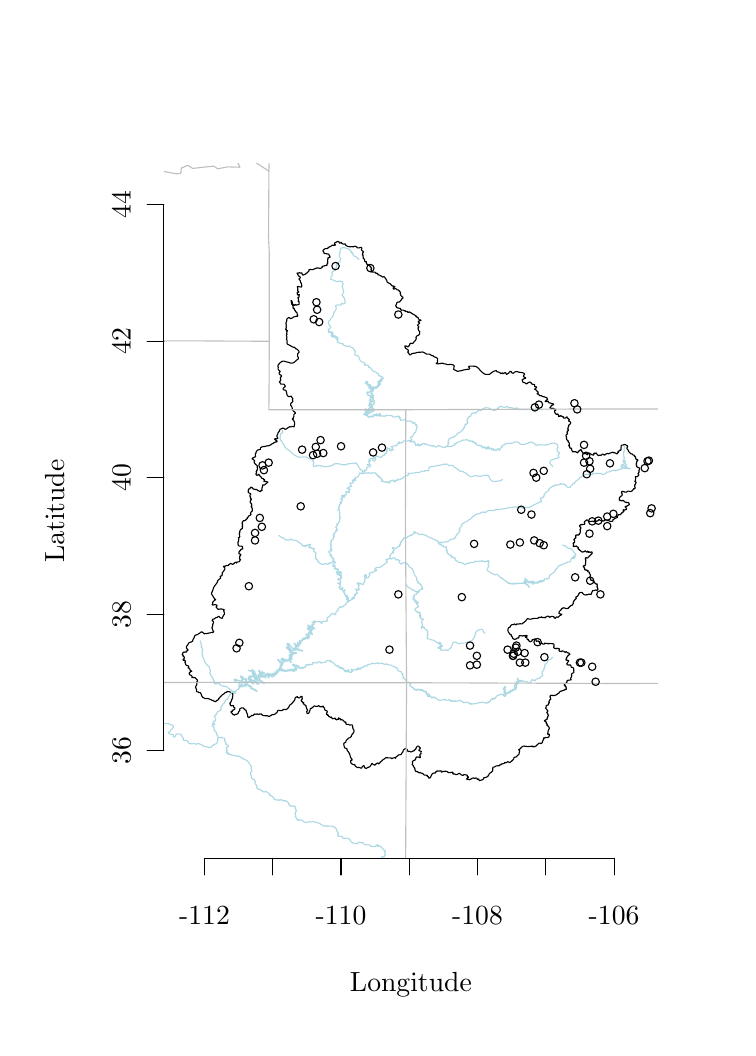
\begin{tikzpicture}[x=1pt,y=1pt]
\definecolor[named]{drawColor}{rgb}{0.00,0.00,0.00}
\definecolor[named]{fillColor}{rgb}{1.00,1.00,1.00}
\fill[color=fillColor,] (0,0) rectangle (252.94,361.35);
\begin{scope}
\path[clip] ( 49.20, 61.20) rectangle (227.75,312.15);

\draw[fill opacity=0.00,draw opacity=0.00,] ( 49.20, 61.20) rectangle (227.74,312.15);
\definecolor[named]{drawColor}{rgb}{0.00,0.00,0.00}

\draw[color=drawColor,line cap=round,line join=round,fill opacity=0.00,] (112.12,284.08) --
	(112.16,284.07) --
	(112.17,284.07) --
	(112.19,284.07) --
	(112.25,284.07) --
	(112.29,284.05) --
	(112.33,284.05) --
	(112.39,284.04) --
	(112.43,284.03) --
	(112.51,283.97) --
	(112.52,283.95) --
	(112.53,283.91) --
	(112.53,283.90) --
	(112.51,283.87) --
	(112.50,283.82) --
	(112.51,283.80) --
	(112.52,283.78) --
	(112.52,283.77) --
	(112.56,283.67) --
	(112.57,283.64) --
	(112.60,283.62) --
	(112.60,283.60) --
	(112.62,283.56) --
	(112.64,283.55) --
	(112.68,283.53) --
	(112.70,283.52) --
	(112.75,283.51) --
	(112.79,283.51) --
	(112.82,283.52) --
	(112.86,283.53) --
	(112.92,283.55) --
	(112.96,283.57) --
	(112.98,283.58) --
	(113.00,283.60) --
	(113.02,283.61) --
	(113.05,283.62) --
	(113.11,283.65) --
	(113.16,283.67) --
	(113.23,283.68) --
	(113.23,283.69) --
	(113.23,283.69) --
	(113.23,283.70) --
	(113.23,283.70) --
	(113.23,283.71) --
	(113.23,283.71) --
	(113.23,283.72) --
	(113.23,283.72) --
	(113.23,283.73) --
	(113.23,283.73) --
	(113.23,283.74) --
	(113.27,283.74) --
	(113.33,283.73) --
	(113.37,283.71) --
	(113.39,283.67) --
	(113.39,283.64) --
	(113.38,283.56) --
	(113.40,283.53) --
	(113.42,283.52) --
	(113.44,283.50) --
	(113.45,283.47) --
	(113.47,283.44) --
	(113.50,283.41) --
	(113.55,283.38) --
	(113.60,283.36) --
	(113.64,283.34) --
	(113.72,283.32) --
	(113.78,283.29) --
	(113.84,283.26) --
	(113.91,283.21) --
	(114.01,283.17) --
	(114.08,283.15) --
	(114.15,283.13) --
	(114.21,283.13) --
	(114.29,283.14) --
	(114.37,283.15) --
	(114.53,283.21) --
	(114.56,283.22) --
	(114.61,283.22) --
	(114.67,283.18) --
	(114.72,283.14) --
	(114.75,283.10) --
	(114.78,283.07) --
	(114.82,283.05) --
	(114.86,283.01) --
	(114.87,282.98) --
	(114.88,282.94) --
	(114.88,282.88) --
	(114.91,282.83) --
	(114.97,282.73) --
	(115.08,282.64) --
	(115.18,282.56) --
	(115.35,282.46) --
	(115.43,282.42) --
	(115.54,282.36) --
	(115.60,282.35) --
	(115.67,282.33) --
	(115.74,282.30) --
	(115.80,282.27) --
	(115.91,282.23) --
	(115.96,282.22) --
	(116.04,282.21) --
	(116.11,282.21) --
	(116.21,282.23) --
	(116.27,282.22) --
	(116.31,282.21) --
	(116.34,282.19) --
	(116.38,282.18) --
	(116.43,282.17) --
	(116.49,282.16) --
	(116.55,282.15) --
	(116.59,282.15) --
	(116.66,282.15) --
	(116.73,282.17) --
	(116.84,282.21) --
	(116.86,282.22) --
	(116.90,282.23) --
	(116.96,282.23) --
	(117.03,282.22) --
	(117.19,282.19) --
	(117.27,282.19) --
	(117.30,282.18) --
	(117.36,282.16) --
	(117.39,282.17) --
	(117.53,282.16) --
	(117.60,282.16) --
	(117.65,282.17) --
	(117.76,282.21) --
	(117.80,282.23) --
	(117.82,282.25) --
	(117.85,282.26) --
	(117.88,282.27) --
	(117.93,282.27) --
	(117.99,282.28) --
	(118.05,282.30) --
	(118.19,282.35) --
	(118.22,282.35) --
	(118.28,282.35) --
	(118.35,282.35) --
	(118.42,282.33) --
	(118.47,282.31) --
	(118.52,282.30) --
	(118.57,282.30) --
	(118.60,282.30) --
	(118.70,282.20) --
	(118.75,282.16) --
	(118.79,282.13) --
	(118.84,282.11) --
	(118.93,282.08) --
	(118.97,282.05) --
	(119.01,282.02) --
	(119.03,281.99) --
	(119.05,281.94) --
	(119.09,281.89) --
	(119.16,281.82) --
	(119.21,281.79) --
	(119.24,281.78) --
	(119.28,281.77) --
	(119.34,281.77) --
	(119.40,281.79) --
	(119.50,281.79) --
	(119.63,281.76) --
	(119.69,281.77) --
	(119.71,281.77) --
	(119.79,281.77) --
	(119.87,281.79) --
	(120.04,281.86) --
	(120.18,281.92) --
	(120.22,281.94) --
	(120.26,281.95) --
	(120.33,281.96) --
	(120.38,281.95) --
	(120.45,281.93) --
	(120.54,281.90) --
	(120.60,281.88) --
	(120.64,281.85) --
	(120.71,281.81) --
	(120.74,281.77) --
	(120.77,281.71) --
	(120.77,281.64) --
	(120.77,281.56) --
	(120.75,281.47) --
	(120.73,281.41) --
	(120.65,281.26) --
	(120.61,281.17) --
	(120.61,281.15) --
	(120.63,281.11) --
	(120.66,281.05) --
	(120.72,280.91) --
	(120.76,280.83) --
	(120.81,280.76) --
	(120.89,280.69) --
	(120.95,280.67) --
	(121.08,280.66) --
	(121.10,280.66) --
	(121.12,280.64) --
	(121.14,280.59) --
	(121.16,280.54) --
	(121.18,280.50) --
	(121.28,280.42) --
	(121.31,280.39) --
	(121.33,280.33) --
	(121.33,280.28) --
	(121.31,280.17) --
	(121.27,280.14) --
	(121.15,280.08) --
	(121.10,280.06) --
	(121.09,280.05) --
	(121.08,280.03) --
	(121.10,279.96) --
	(121.09,279.89) --
	(121.08,279.82) --
	(121.04,279.70) --
	(121.04,279.67) --
	(121.05,279.64) --
	(121.07,279.61) --
	(121.09,279.59) --
	(121.11,279.56) --
	(121.14,279.50) --
	(121.14,279.46) --
	(121.10,279.42) --
	(121.00,279.34) --
	(120.91,279.28) --
	(120.90,279.26) --
	(120.91,279.23) --
	(120.94,279.20) --
	(120.98,279.18) --
	(121.03,279.17) --
	(121.08,279.14) --
	(121.11,279.12) --
	(121.16,279.06) --
	(121.19,279.02) --
	(121.20,278.97) --
	(121.20,278.91) --
	(121.20,278.82) --
	(121.21,278.76) --
	(121.21,278.71) --
	(121.20,278.65) --
	(121.18,278.59) --
	(121.18,278.57) --
	(121.22,278.54) --
	(121.24,278.51) --
	(121.25,278.48) --
	(121.24,278.43) --
	(121.24,278.37) --
	(121.24,278.31) --
	(121.23,278.25) --
	(121.22,278.13) --
	(121.22,278.09) --
	(121.23,278.06) --
	(121.25,278.03) --
	(121.31,278.01) --
	(121.37,277.97) --
	(121.47,277.85) --
	(121.49,277.79) --
	(121.52,277.76) --
	(121.58,277.73) --
	(121.60,277.71) --
	(121.63,277.66) --
	(121.67,277.59) --
	(121.71,277.49) --
	(121.74,277.42) --
	(121.75,277.37) --
	(121.76,277.30) --
	(121.76,277.25) --
	(121.75,277.20) --
	(121.74,277.10) --
	(121.74,277.04) --
	(121.76,277.00) --
	(121.80,276.95) --
	(121.84,276.91) --
	(121.86,276.86) --
	(121.89,276.83) --
	(121.91,276.82) --
	(121.94,276.81) --
	(121.96,276.80) --
	(122.05,276.80) --
	(122.09,276.80) --
	(122.16,276.82) --
	(122.22,276.81) --
	(122.35,276.78) --
	(122.37,276.76) --
	(122.37,276.74) --
	(122.36,276.70) --
	(122.35,276.64) --
	(122.33,276.54) --
	(122.32,276.49) --
	(122.32,276.44) --
	(122.35,276.33) --
	(122.40,276.23) --
	(122.42,276.20) --
	(122.44,276.18) --
	(122.46,276.15) --
	(122.48,276.10) --
	(122.51,276.03) --
	(122.54,275.96) --
	(122.57,275.88) --
	(122.58,275.86) --
	(122.60,275.84) --
	(122.64,275.83) --
	(122.68,275.83) --
	(122.72,275.82) --
	(122.79,275.82) --
	(122.83,275.81) --
	(122.90,275.77) --
	(122.93,275.74) --
	(122.95,275.72) --
	(123.00,275.70) --
	(123.06,275.69) --
	(123.11,275.69) --
	(123.20,275.65) --
	(123.30,275.57) --
	(123.45,275.43) --
	(123.52,275.32) --
	(123.56,275.24) --
	(123.58,275.23) --
	(123.61,275.23) --
	(123.68,275.22) --
	(123.73,275.23) --
	(123.78,275.23) --
	(123.80,275.20) --
	(123.82,275.16) --
	(123.83,275.13) --
	(123.84,275.09) --
	(123.84,275.06) --
	(123.84,275.02) --
	(123.85,275.00) --
	(123.87,274.96) --
	(123.91,274.92) --
	(123.97,274.89) --
	(124.01,274.85) --
	(124.04,274.79) --
	(124.05,274.76) --
	(124.05,274.72) --
	(124.05,274.69) --
	(124.06,274.65) --
	(124.08,274.61) --
	(124.12,274.56) --
	(124.20,274.53) --
	(124.22,274.50) --
	(124.22,274.45) --
	(124.23,274.38) --
	(124.23,274.32) --
	(124.24,274.28) --
	(124.24,274.24) --
	(124.19,274.19) --
	(124.12,274.12) --
	(124.06,274.06) --
	(124.04,274.05) --
	(124.03,274.04) --
	(124.03,274.03) --
	(124.03,274.01) --
	(124.05,273.97) --
	(124.07,273.91) --
	(124.08,273.84) --
	(124.12,273.73) --
	(124.14,273.69) --
	(124.17,273.66) --
	(124.22,273.62) --
	(124.24,273.58) --
	(124.25,273.55) --
	(124.24,273.51) --
	(124.23,273.48) --
	(124.21,273.42) --
	(124.19,273.35) --
	(124.18,273.31) --
	(124.19,273.27) --
	(124.21,273.22) --
	(124.25,273.13) --
	(124.25,273.08) --
	(124.26,273.07) --
	(124.29,273.06) --
	(124.33,273.05) --
	(124.41,273.04) --
	(124.47,273.02) --
	(124.50,273.02) --
	(124.60,273.06) --
	(124.70,273.09) --
	(124.74,273.09) --
	(124.81,273.08) --
	(124.89,273.05) --
	(124.92,273.03) --
	(124.95,273.00) --
	(124.97,272.99) --
	(125.00,272.99) --
	(125.03,273.00) --
	(125.07,273.01) --
	(125.10,273.01) --
	(125.20,273.00) --
	(125.32,272.99) --
	(125.43,272.99) --
	(125.49,272.98) --
	(125.55,272.95) --
	(125.57,272.93) --
	(125.59,272.90) --
	(125.60,272.86) --
	(125.63,272.84) --
	(125.66,272.81) --
	(125.69,272.79) --
	(125.72,272.76) --
	(125.73,272.75) --
	(125.73,272.75) --
	(125.72,272.75) --
	(125.72,272.75) --
	(125.71,272.75) --
	(125.71,272.75) --
	(125.71,272.71) --
	(125.73,272.69) --
	(125.75,272.65) --
	(125.85,272.61) --
	(125.93,272.60) --
	(125.97,272.60) --
	(126.11,272.62) --
	(126.15,272.62) --
	(126.17,272.62) --
	(126.20,272.60) --
	(126.27,272.52) --
	(126.28,272.51) --
	(126.30,272.50) --
	(126.33,272.51) --
	(126.37,272.53) --
	(126.40,272.54) --
	(126.42,272.53) --
	(126.46,272.52) --
	(126.49,272.50) --
	(126.51,272.46) --
	(126.51,272.44) --
	(126.51,272.41) --
	(126.49,272.38) --
	(126.48,272.33) --
	(126.48,272.30) --
	(126.58,272.16) --
	(126.64,272.11) --
	(126.66,272.06) --
	(126.68,272.05) --
	(126.70,272.04) --
	(126.71,272.04) --
	(126.77,272.05) --
	(126.85,272.03) --
	(126.88,272.01) --
	(126.94,271.98) --
	(126.99,271.96) --
	(127.04,271.96) --
	(127.16,271.95) --
	(127.19,271.94) --
	(127.21,271.93) --
	(127.36,271.76) --
	(127.40,271.73) --
	(127.46,271.71) --
	(127.66,271.66) --
	(127.69,271.66) --
	(127.72,271.65) --
	(127.91,271.51) --
	(128.00,271.44) --
	(128.03,271.41) --
	(128.06,271.34) --
	(128.07,271.31) --
	(128.08,271.29) --
	(128.10,271.27) --
	(128.12,271.26) --
	(128.16,271.26) --
	(128.31,271.26) --
	(128.38,271.27) --
	(128.47,271.28) --
	(128.49,271.29) --
	(128.57,271.34) --
	(128.70,271.42) --
	(128.72,271.42) --
	(128.73,271.42) --
	(128.74,271.41) --
	(128.75,271.40) --
	(128.76,271.37) --
	(128.85,271.29) --
	(128.96,271.21) --
	(128.99,271.17) --
	(129.03,271.13) --
	(129.10,270.96) --
	(129.14,270.91) --
	(129.24,270.82) --
	(129.33,270.76) --
	(129.37,270.74) --
	(129.43,270.60) --
	(129.46,270.50) --
	(129.47,270.43) --
	(129.50,270.37) --
	(129.51,270.34) --
	(129.55,270.26) --
	(129.58,270.23) --
	(129.63,270.20) --
	(129.70,270.17) --
	(129.72,270.15) --
	(129.76,270.04) --
	(129.78,269.92) --
	(129.78,269.84) --
	(129.77,269.71) --
	(129.78,269.68) --
	(129.86,269.54) --
	(129.94,269.40) --
	(129.99,269.35) --
	(130.03,269.27) --
	(130.06,269.23) --
	(130.08,269.22) --
	(130.12,269.20) --
	(130.35,269.14) --
	(130.40,269.12) --
	(130.44,269.10) --
	(130.49,269.07) --
	(130.54,269.02) --
	(130.59,269.00) --
	(130.63,268.97) --
	(130.69,268.96) --
	(130.78,268.94) --
	(130.84,268.94) --
	(130.87,268.93) --
	(130.90,268.91) --
	(130.95,268.89) --
	(131.00,268.82) --
	(131.02,268.76) --
	(131.05,268.73) --
	(131.12,268.68) --
	(131.18,268.63) --
	(131.20,268.59) --
	(131.21,268.56) --
	(131.21,268.49) --
	(131.22,268.47) --
	(131.24,268.44) --
	(131.28,268.42) --
	(131.33,268.41) --
	(131.39,268.40) --
	(131.41,268.39) --
	(131.43,268.38) --
	(131.46,268.30) --
	(131.51,268.20) --
	(131.55,268.15) --
	(131.58,268.15) --
	(131.61,268.13) --
	(131.74,268.02) --
	(131.77,268.00) --
	(131.81,267.96) --
	(131.87,267.94) --
	(131.89,267.94) --
	(131.91,267.95) --
	(131.93,267.99) --
	(131.97,268.03) --
	(132.02,268.05) --
	(132.04,268.05) --
	(132.07,268.05) --
	(132.10,268.02) --
	(132.17,267.96) --
	(132.20,267.94) --
	(132.25,267.92) --
	(132.38,267.89) --
	(132.51,267.87) --
	(132.54,267.87) --
	(132.58,267.84) --
	(132.62,267.79) --
	(132.64,267.76) --
	(132.65,267.73) --
	(132.68,267.69) --
	(132.68,267.66) --
	(132.65,267.64) --
	(132.60,267.63) --
	(132.55,267.62) --
	(132.51,267.60) --
	(132.45,267.61) --
	(132.41,267.61) --
	(132.39,267.60) --
	(132.36,267.58) --
	(132.34,267.56) --
	(132.32,267.54) --
	(132.29,267.49) --
	(132.25,267.45) --
	(132.20,267.43) --
	(132.17,267.40) --
	(132.12,267.35) --
	(132.07,267.27) --
	(132.04,267.25) --
	(132.04,267.21) --
	(132.05,267.19) --
	(132.07,267.16) --
	(132.08,267.13) --
	(132.08,267.11) --
	(132.06,267.08) --
	(132.06,267.06) --
	(132.06,267.04) --
	(132.07,267.02) --
	(132.16,266.96) --
	(132.25,266.92) --
	(132.31,266.89) --
	(132.40,266.89) --
	(132.44,266.89) --
	(132.48,266.90) --
	(132.51,266.91) --
	(132.55,266.94) --
	(132.63,267.01) --
	(132.72,267.07) --
	(132.76,267.09) --
	(132.80,267.09) --
	(132.84,267.09) --
	(132.92,267.06) --
	(132.97,267.05) --
	(133.06,267.03) --
	(133.08,267.01) --
	(133.12,266.98) --
	(133.18,266.94) --
	(133.28,266.89) --
	(133.31,266.86) --
	(133.35,266.79) --
	(133.38,266.74) --
	(133.41,266.70) --
	(133.44,266.67) --
	(133.49,266.64) --
	(133.75,266.58) --
	(133.87,266.54) --
	(133.91,266.53) --
	(133.95,266.52) --
	(133.98,266.50) --
	(134.01,266.46) --
	(134.03,266.44) --
	(134.15,266.39) --
	(134.19,266.36) --
	(134.24,266.31) --
	(134.28,266.26) --
	(134.29,266.23) --
	(134.29,266.10) --
	(134.31,266.05) --
	(134.32,266.03) --
	(134.35,266.00) --
	(134.41,265.97) --
	(134.52,265.93) --
	(134.55,265.91) --
	(134.57,265.88) --
	(134.59,265.84) --
	(134.63,265.77) --
	(134.66,265.67) --
	(134.68,265.64) --
	(134.76,265.54) --
	(134.75,265.52) --
	(134.70,265.48) --
	(134.64,265.40) --
	(134.61,265.32) --
	(134.60,265.27) --
	(134.60,265.25) --
	(134.61,265.21) --
	(134.62,265.18) --
	(134.73,265.01) --
	(134.76,264.95) --
	(134.77,264.89) --
	(134.77,264.80) --
	(134.76,264.76) --
	(134.77,264.73) --
	(134.79,264.70) --
	(134.83,264.61) --
	(134.88,264.55) --
	(135.02,264.43) --
	(135.15,264.33) --
	(135.18,264.30) --
	(135.21,264.26) --
	(135.25,264.14) --
	(135.29,264.09) --
	(135.32,264.07) --
	(135.37,264.05) --
	(135.41,264.04) --
	(135.46,264.02) --
	(135.51,264.00) --
	(135.57,263.95) --
	(135.59,263.92) --
	(135.60,263.90) --
	(135.61,263.85) --
	(135.60,263.80) --
	(135.58,263.76) --
	(135.58,263.72) --
	(135.59,263.69) --
	(135.60,263.62) --
	(135.59,263.59) --
	(135.57,263.57) --
	(135.55,263.55) --
	(135.46,263.49) --
	(135.29,263.43) --
	(135.24,263.42) --
	(135.19,263.39) --
	(135.14,263.35) --
	(135.10,263.30) --
	(135.09,263.26) --
	(135.10,263.23) --
	(135.13,263.17) --
	(135.13,263.09) --
	(135.13,263.07) --
	(135.13,263.03) --
	(135.11,263.01) --
	(134.99,262.94) --
	(134.81,262.80) --
	(134.76,262.76) --
	(134.70,262.72) --
	(134.66,262.68) --
	(134.63,262.63) --
	(134.61,262.56) --
	(134.59,262.51) --
	(134.59,262.49) --
	(134.56,262.46) --
	(134.53,262.42) --
	(134.45,262.30) --
	(134.38,262.26) --
	(134.34,262.23) --
	(134.28,262.22) --
	(134.16,262.23) --
	(134.08,262.23) --
	(134.04,262.22) --
	(133.97,262.19) --
	(133.89,262.18) --
	(133.62,262.13) --
	(133.56,262.10) --
	(133.46,261.97) --
	(133.43,261.95) --
	(133.38,261.92) --
	(133.36,261.91) --
	(133.36,261.89) --
	(133.36,261.85) --
	(133.36,261.81) --
	(133.35,261.78) --
	(133.32,261.72) --
	(133.31,261.62) --
	(133.30,261.53) --
	(133.29,261.50) --
	(133.24,261.41) --
	(133.18,261.32) --
	(133.16,261.27) --
	(133.07,261.02) --
	(132.98,260.90) --
	(132.97,260.85) --
	(132.97,260.82) --
	(132.97,260.80) --
	(132.98,260.75) --
	(133.02,260.72) --
	(133.10,260.68) --
	(133.17,260.64) --
	(133.24,260.59) --
	(133.26,260.55) --
	(133.26,260.49) --
	(133.25,260.39) --
	(133.24,260.34) --
	(133.24,260.31) --
	(133.25,260.28) --
	(133.27,260.24) --
	(133.32,260.20) --
	(133.38,260.17) --
	(133.59,260.14) --
	(133.64,260.13) --
	(133.72,260.07) --
	(133.77,260.05) --
	(133.84,260.05) --
	(133.98,260.04) --
	(134.11,260.01) --
	(134.21,259.97) --
	(134.34,259.91) --
	(134.40,259.88) --
	(134.49,259.86) --
	(134.64,259.86) --
	(134.68,259.86) --
	(134.70,259.85) --
	(134.72,259.83) --
	(134.74,259.81) --
	(134.80,259.64) --
	(134.81,259.59) --
	(134.82,259.55) --
	(134.81,259.52) --
	(134.80,259.49) --
	(134.80,259.46) --
	(134.85,259.40) --
	(134.89,259.32) --
	(134.91,259.29) --
	(134.95,259.27) --
	(135.01,259.25) --
	(135.07,259.25) --
	(135.14,259.26) --
	(135.25,259.30) --
	(135.29,259.30) --
	(135.33,259.30) --
	(135.47,259.27) --
	(135.54,259.27) --
	(135.57,259.27) --
	(135.65,259.30) --
	(135.69,259.30) --
	(135.72,259.30) --
	(135.76,259.29) --
	(135.79,259.28) --
	(135.86,259.20) --
	(135.91,259.17) --
	(135.96,259.15) --
	(136.03,259.14) --
	(136.20,259.12) --
	(136.35,259.09) --
	(136.39,259.07) --
	(136.46,259.03) --
	(136.46,259.00) --
	(136.47,258.94) --
	(136.45,258.87) --
	(136.43,258.82) --
	(136.44,258.80) --
	(136.50,258.78) --
	(136.57,258.77) --
	(136.65,258.79) --
	(136.73,258.81) --
	(136.78,258.80) --
	(136.82,258.79) --
	(136.89,258.80) --
	(136.94,258.81) --
	(137.05,258.82) --
	(137.10,258.82) --
	(137.15,258.80) --
	(137.18,258.78) --
	(137.26,258.71) --
	(137.31,258.64) --
	(137.34,258.49) --
	(137.36,258.47) --
	(137.39,258.47) --
	(137.43,258.48) --
	(137.47,258.47) --
	(137.54,258.48) --
	(137.57,258.49) --
	(137.67,258.53) --
	(137.80,258.60) --
	(137.83,258.62) --
	(137.85,258.65) --
	(137.86,258.66) --
	(137.88,258.67) --
	(138.06,258.65) --
	(138.10,258.63) --
	(138.12,258.62) --
	(138.14,258.50) --
	(138.16,258.45) --
	(138.16,258.41) --
	(138.18,258.38) --
	(138.21,258.36) --
	(138.26,258.35) --
	(138.34,258.34) --
	(138.39,258.34) --
	(138.47,258.33) --
	(138.55,258.31) --
	(138.63,258.28) --
	(138.65,258.27) --
	(138.74,258.16) --
	(138.85,258.07) --
	(139.14,257.86) --
	(139.38,257.74) --
	(139.48,257.72) --
	(139.52,257.70) --
	(139.60,257.65) --
	(139.66,257.62) --
	(139.74,257.57) --
	(139.80,257.54) --
	(140.07,257.35) --
	(140.35,257.16) --
	(140.43,257.10) --
	(140.48,257.05) --
	(140.50,257.03) --
	(140.50,257.01) --
	(140.49,257.00) --
	(140.46,256.98) --
	(140.41,256.97) --
	(140.35,256.97) --
	(140.31,256.97) --
	(140.30,256.96) --
	(140.29,256.93) --
	(140.30,256.91) --
	(140.33,256.89) --
	(140.38,256.87) --
	(140.62,256.78) --
	(140.83,256.71) --
	(140.91,256.68) --
	(140.97,256.66) --
	(141.02,256.63) --
	(141.10,256.54) --
	(141.13,256.45) --
	(141.13,256.35) --
	(141.15,256.29) --
	(141.19,256.21) --
	(141.23,256.14) --
	(141.29,256.06) --
	(141.39,255.94) --
	(141.43,255.88) --
	(141.46,255.84) --
	(141.49,255.81) --
	(141.53,255.78) --
	(141.56,255.76) --
	(141.62,255.75) --
	(141.72,255.75) --
	(141.90,255.75) --
	(141.97,255.73) --
	(142.06,255.68) --
	(142.12,255.63) --
	(142.13,255.62) --
	(142.13,255.59) --
	(142.10,255.57) --
	(142.03,255.56) --
	(141.91,255.53) --
	(141.74,255.46) --
	(141.65,255.41) --
	(141.59,255.38) --
	(141.51,255.36) --
	(141.34,255.30) --
	(141.22,255.23) --
	(141.15,255.15) --
	(141.13,255.10) --
	(141.12,255.06) --
	(141.12,255.03) --
	(141.15,255.01) --
	(141.21,254.98) --
	(141.28,254.95) --
	(141.33,254.91) --
	(141.37,254.85) --
	(141.42,254.81) --
	(141.47,254.76) --
	(141.55,254.70) --
	(141.57,254.68) --
	(141.59,254.65) --
	(141.60,254.62) --
	(141.62,254.57) --
	(141.62,254.53) --
	(141.63,254.51) --
	(141.58,254.48) --
	(141.52,254.43) --
	(141.48,254.39) --
	(141.30,254.28) --
	(141.23,254.22) --
	(141.17,254.14) --
	(141.02,254.03) --
	(140.98,253.98) --
	(140.96,253.94) --
	(140.96,253.92) --
	(140.96,253.88) --
	(140.99,253.83) --
	(140.99,253.82) --
	(140.98,253.79) --
	(140.95,253.76) --
	(140.95,253.69) --
	(140.95,253.66) --
	(140.97,253.63) --
	(141.00,253.60) --
	(141.11,253.52) --
	(141.23,253.42) --
	(141.29,253.37) --
	(141.31,253.34) --
	(141.32,253.31) --
	(141.32,253.25) --
	(141.31,253.17) --
	(141.29,253.12) --
	(141.26,253.07) --
	(141.24,253.03) --
	(141.21,252.99) --
	(141.14,252.91) --
	(141.10,252.89) --
	(141.08,252.87) --
	(141.05,252.83) --
	(141.04,252.81) --
	(141.04,252.78) --
	(141.07,252.66) --
	(141.11,252.53) --
	(141.13,252.48) --
	(141.15,252.32) --
	(141.18,252.22) --
	(141.23,252.05) --
	(141.28,251.92) --
	(141.33,251.85) --
	(141.42,251.76) --
	(141.50,251.70) --
	(141.55,251.65) --
	(141.65,251.59) --
	(141.67,251.57) --
	(141.69,251.56) --
	(141.69,251.49) --
	(141.70,251.45) --
	(141.68,251.40) --
	(141.66,251.35) --
	(141.65,251.29) --
	(141.63,251.21) --
	(141.63,250.92) --
	(141.62,250.84) --
	(141.62,250.71) --
	(141.61,250.63) --
	(141.59,250.60) --
	(141.43,250.43) --
	(141.39,250.38) --
	(141.37,250.34) --
	(141.35,250.31) --
	(141.29,250.26) --
	(141.22,250.21) --
	(141.16,250.18) --
	(140.91,250.07) --
	(140.81,250.03) --
	(140.74,249.98) --
	(140.60,249.89) --
	(140.56,249.84) --
	(140.53,249.80) --
	(140.47,249.73) --
	(140.40,249.60) --
	(140.34,249.48) --
	(140.30,249.34) --
	(140.30,249.29) --
	(140.30,249.26) --
	(140.32,249.24) --
	(140.37,249.18) --
	(140.41,249.13) --
	(140.42,249.10) --
	(140.42,249.05) --
	(140.39,248.99) --
	(140.37,248.94) --
	(140.36,248.90) --
	(140.32,248.69) --
	(140.29,248.62) --
	(140.26,248.58) --
	(140.21,248.48) --
	(140.17,248.39) --
	(139.91,248.08) --
	(139.90,248.08) --
	(139.90,248.08) --
	(139.89,248.08) --
	(139.89,248.08) --
	(139.88,248.08) --
	(139.88,248.08) --
	(139.87,248.08) --
	(139.87,248.08) --
	(139.86,248.08) --
	(139.86,248.08) --
	(139.85,248.08) --
	(139.85,248.08) --
	(139.84,248.08) --
	(139.84,248.08) --
	(139.83,248.08) --
	(139.82,248.07) --
	(139.64,247.97) --
	(139.62,247.88) --
	(139.61,247.86) --
	(139.59,247.76) --
	(139.56,247.68) --
	(139.53,247.65) --
	(139.50,247.61) --
	(139.50,247.59) --
	(139.48,247.59) --
	(139.44,247.55) --
	(139.39,247.50) --
	(139.37,247.49) --
	(139.35,247.47) --
	(139.33,247.45) --
	(139.32,247.43) --
	(139.30,247.37) --
	(139.24,247.33) --
	(139.17,247.29) --
	(139.08,247.25) --
	(139.00,247.23) --
	(138.97,247.23) --
	(138.92,247.24) --
	(138.89,247.24) --
	(138.87,247.26) --
	(138.76,247.26) --
	(138.70,247.26) --
	(138.67,247.26) --
	(138.60,247.28) --
	(138.55,247.31) --
	(138.44,247.32) --
	(138.41,247.31) --
	(138.39,247.30) --
	(138.34,247.28) --
	(138.31,247.24) --
	(138.27,247.21) --
	(138.21,247.18) --
	(138.18,247.17) --
	(138.11,247.16) --
	(138.09,247.13) --
	(138.08,247.11) --
	(138.08,246.91) --
	(138.06,246.78) --
	(138.02,246.67) --
	(137.97,246.58) --
	(137.91,246.50) --
	(137.85,246.44) --
	(137.72,246.34) --
	(137.63,246.26) --
	(137.61,246.25) --
	(137.60,246.23) --
	(137.48,246.09) --
	(137.46,246.08) --
	(137.44,246.06) --
	(137.38,246.05) --
	(137.33,246.05) --
	(137.30,246.05) --
	(137.22,246.08) --
	(137.18,246.10) --
	(137.15,246.11) --
	(137.06,246.15) --
	(136.97,246.20) --
	(136.71,246.30) --
	(136.56,246.34) --
	(136.37,246.38) --
	(136.31,246.36) --
	(136.30,246.35) --
	(136.29,246.33) --
	(136.30,246.27) --
	(136.33,246.19) --
	(136.33,246.17) --
	(136.33,246.12) --
	(136.33,246.06) --
	(136.33,246.02) --
	(136.33,245.98) --
	(136.34,245.94) --
	(136.36,245.84) --
	(136.38,245.80) --
	(136.42,245.72) --
	(136.45,245.67) --
	(136.57,245.55) --
	(136.59,245.52) --
	(136.61,245.51) --
	(136.61,245.49) --
	(136.63,245.47) --
	(136.69,245.42) --
	(136.72,245.39) --
	(136.77,245.37) --
	(136.88,245.31) --
	(136.92,245.28) --
	(136.98,245.24) --
	(137.04,245.21) --
	(137.07,245.19) --
	(137.14,245.12) --
	(137.25,245.05) --
	(137.36,244.96) --
	(137.43,244.90) --
	(137.46,244.84) --
	(137.47,244.78) --
	(137.48,244.72) --
	(137.50,244.70) --
	(137.57,244.64) --
	(137.59,244.61) --
	(137.59,244.60) --
	(137.59,244.59) --
	(137.59,244.57) --
	(137.52,244.41) --
	(137.50,244.40) --
	(137.50,244.37) --
	(137.49,244.36) --
	(137.47,244.34) --
	(137.45,244.30) --
	(137.43,244.29) --
	(137.39,244.23) --
	(137.37,244.22) --
	(137.34,244.18) --
	(137.34,244.13) --
	(137.34,244.13) --
	(137.36,244.09) --
	(137.39,244.03) --
	(137.43,244.00) --
	(137.47,243.95) --
	(137.53,243.88) --
	(137.64,243.77) --
	(137.69,243.72) --
	(137.76,243.65) --
	(137.79,243.60) --
	(137.81,243.53) --
	(137.82,243.52) --
	(137.84,243.50) --
	(137.84,243.48) --
	(137.89,243.39) --
	(137.94,243.29) --
	(137.94,243.27) --
	(137.95,243.23) --
	(137.97,243.19) --
	(138.02,243.14) --
	(138.07,243.12) --
	(138.10,243.11) --
	(138.13,243.11) --
	(138.29,243.13) --
	(138.42,243.15) --
	(138.44,243.16) --
	(138.46,243.18) --
	(138.49,243.22) --
	(138.51,243.26) --
	(138.54,243.29) --
	(138.56,243.31) --
	(138.58,243.33) --
	(138.62,243.38) --
	(138.63,243.40) --
	(138.65,243.42) --
	(138.67,243.46) --
	(138.70,243.47) --
	(138.74,243.52) --
	(138.77,243.54) --
	(138.85,243.55) --
	(138.90,243.55) --
	(138.96,243.55) --
	(138.99,243.56) --
	(139.01,243.57) --
	(139.04,243.60) --
	(139.16,243.65) --
	(139.22,243.67) --
	(139.29,243.68) --
	(139.46,243.69) --
	(139.81,243.72) --
	(139.92,243.74) --
	(139.94,243.74) --
	(140.00,243.75) --
	(140.11,243.78) --
	(140.16,243.78) --
	(140.19,243.79) --
	(140.22,243.79) --
	(140.24,243.81) --
	(140.29,243.82) --
	(140.39,243.85) --
	(140.53,243.92) --
	(140.57,243.94) --
	(140.65,243.97) --
	(140.72,244.00) --
	(140.80,244.01) --
	(140.93,244.03) --
	(141.34,244.05) --
	(141.50,244.05) --
	(141.61,244.05) --
	(141.97,244.07) --
	(142.05,244.08) --
	(142.22,244.10) --
	(142.34,244.13) --
	(142.37,244.13) --
	(142.39,244.14) --
	(142.53,244.15) --
	(142.62,244.15) --
	(142.70,244.14) --
	(142.78,244.12) --
	(142.90,244.08) --
	(142.99,244.05) --
	(143.14,243.97) --
	(143.21,243.93) --
	(143.25,243.91) --
	(143.48,243.79) --
	(143.63,243.70) --
	(143.71,243.64) --
	(143.77,243.60) --
	(143.80,243.59) --
	(143.91,243.52) --
	(143.95,243.50) --
	(144.10,243.42) --
	(144.15,243.40) --
	(144.20,243.38) --
	(144.28,243.36) --
	(144.50,243.36) --
	(144.56,243.36) --
	(144.67,243.36) --
	(144.86,243.36) --
	(144.91,243.36) --
	(144.99,243.38) --
	(145.16,243.39) --
	(145.21,243.39) --
	(145.32,243.37) --
	(145.36,243.35) --
	(145.40,243.32) --
	(145.46,243.28) --
	(145.47,243.26) --
	(145.51,243.23) --
	(145.60,243.14) --
	(145.62,243.12) --
	(145.63,243.11) --
	(145.73,243.03) --
	(145.78,243.00) --
	(145.78,242.99) --
	(145.78,242.99) --
	(145.80,242.97) --
	(145.84,242.95) --
	(145.87,242.94) --
	(145.89,242.93) --
	(145.97,242.90) --
	(146.02,242.88) --
	(146.04,242.88) --
	(146.06,242.86) --
	(146.16,242.83) --
	(146.24,242.81) --
	(146.27,242.80) --
	(146.37,242.79) --
	(146.46,242.79) --
	(146.48,242.78) --
	(146.50,242.77) --
	(146.56,242.73) --
	(146.61,242.68) --
	(146.64,242.64) --
	(146.68,242.57) --
	(146.69,242.55) --
	(146.72,242.51) --
	(146.80,242.46) --
	(146.87,242.42) --
	(147.06,242.35) --
	(147.30,242.29) --
	(147.32,242.28) --
	(147.40,242.25) --
	(147.43,242.24) --
	(147.53,242.20) --
	(147.56,242.19) --
	(147.60,242.17) --
	(147.64,242.14) --
	(147.71,242.11) --
	(147.78,242.07) --
	(147.84,242.03) --
	(147.98,241.91) --
	(147.99,241.89) --
	(148.01,241.87) --
	(148.06,241.80) --
	(148.11,241.70) --
	(148.11,241.68) --
	(148.13,241.64) --
	(148.14,241.61) --
	(148.14,241.57) --
	(148.14,241.50) --
	(148.11,241.36) --
	(148.07,241.12) --
	(148.07,241.10) --
	(148.07,240.93) --
	(148.07,240.85) --
	(148.07,240.83) --
	(148.08,240.81) --
	(148.09,240.77) --
	(148.10,240.73) --
	(148.11,240.68) --
	(148.12,240.47) --
	(148.12,240.43) --
	(148.10,240.41) --
	(147.99,240.32) --
	(147.95,240.29) --
	(147.91,240.26) --
	(147.83,240.21) --
	(147.74,240.15) --
	(147.68,240.12) --
	(147.66,240.10) --
	(147.64,240.08) --
	(147.64,240.04) --
	(147.65,240.02) --
	(147.66,240.00) --
	(147.67,239.99) --
	(147.72,239.97) --
	(147.78,239.95) --
	(147.80,239.94) --
	(147.90,239.91) --
	(148.11,239.88) --
	(148.17,239.88) --
	(148.22,239.87) --
	(148.33,239.88) --
	(148.42,239.89) --
	(148.55,239.91) --
	(148.82,239.94) --
	(148.98,239.97) --
	(149.37,240.05) --
	(149.51,240.07) --
	(149.61,240.09) --
	(149.69,240.10) --
	(149.81,240.10) --
	(149.86,240.09) --
	(150.09,240.05) --
	(150.12,240.04) --
	(150.21,240.01) --
	(150.24,240.00) --
	(150.29,239.98) --
	(150.31,239.94) --
	(150.35,239.91) --
	(150.41,239.87) --
	(150.43,239.86) --
	(150.51,239.84) --
	(150.57,239.83) --
	(150.78,239.86) --
	(150.84,239.86) --
	(150.95,239.85) --
	(151.00,239.84) --
	(151.08,239.82) --
	(151.20,239.78) --
	(151.34,239.72) --
	(151.39,239.69) --
	(151.41,239.69) --
	(151.43,239.68) --
	(151.56,239.64) --
	(151.69,239.61) --
	(151.79,239.59) --
	(151.96,239.57) --
	(152.10,239.57) --
	(152.12,239.57) --
	(152.15,239.57) --
	(152.25,239.59) --
	(152.31,239.61) --
	(152.59,239.67) --
	(152.70,239.68) --
	(152.72,239.68) --
	(152.73,239.68) --
	(152.78,239.69) --
	(152.84,239.69) --
	(152.85,239.68) --
	(152.88,239.68) --
	(152.92,239.69) --
	(153.01,239.67) --
	(153.09,239.66) --
	(153.14,239.65) --
	(153.16,239.65) --
	(153.19,239.64) --
	(153.24,239.62) --
	(153.29,239.61) --
	(153.32,239.60) --
	(153.39,239.58) --
	(153.47,239.55) --
	(153.59,239.51) --
	(153.69,239.48) --
	(153.79,239.44) --
	(153.86,239.41) --
	(153.93,239.38) --
	(153.94,239.36) --
	(153.98,239.33) --
	(154.02,239.30) --
	(154.03,239.26) --
	(154.09,239.19) --
	(154.12,239.11) --
	(154.14,239.03) --
	(154.14,238.99) --
	(154.12,238.91) --
	(154.09,238.86) --
	(154.04,238.76) --
	(154.04,238.72) --
	(154.02,238.66) --
	(154.03,238.62) --
	(154.03,238.59) --
	(154.03,238.46) --
	(154.04,238.43) --
	(154.03,238.39) --
	(154.03,238.36) --
	(153.99,238.24) --
	(153.96,238.15) --
	(153.95,237.99) --
	(153.95,237.97) --
	(153.96,237.93) --
	(153.98,237.83) --
	(154.01,237.80) --
	(154.07,237.75) --
	(154.24,237.69) --
	(154.39,237.63) --
	(154.54,237.56) --
	(154.59,237.54) --
	(154.65,237.50) --
	(154.83,237.40) --
	(154.96,237.33) --
	(155.03,237.30) --
	(155.10,237.27) --
	(155.15,237.25) --
	(155.18,237.23) --
	(155.21,237.22) --
	(155.23,237.22) --
	(155.25,237.20) --
	(155.33,237.16) --
	(155.34,237.16) --
	(155.39,237.17) --
	(155.47,237.18) --
	(155.69,237.23) --
	(155.71,237.24) --
	(155.74,237.24) --
	(155.79,237.25) --
	(155.84,237.25) --
	(155.87,237.25) --
	(155.94,237.27) --
	(156.02,237.29) --
	(156.04,237.30) --
	(156.15,237.33) --
	(156.33,237.35) --
	(156.41,237.37) --
	(156.50,237.38) --
	(156.63,237.39) --
	(156.68,237.40) --
	(156.73,237.42) --
	(156.83,237.44) --
	(156.88,237.46) --
	(156.94,237.48) --
	(157.11,237.53) --
	(157.15,237.56) --
	(157.18,237.56) --
	(157.23,237.58) --
	(157.35,237.62) --
	(157.59,237.67) --
	(157.62,237.68) --
	(157.69,237.69) --
	(157.78,237.70) --
	(157.81,237.70) --
	(157.94,237.72) --
	(158.15,237.77) --
	(158.26,237.79) --
	(158.31,237.80) --
	(158.34,237.80) --
	(158.39,237.82) --
	(158.62,237.86) --
	(158.81,237.90) --
	(158.89,237.91) --
	(158.95,237.90) --
	(159.03,237.90) --
	(159.08,237.89) --
	(159.16,237.89) --
	(159.22,237.89) --
	(159.33,237.90) --
	(159.35,237.90) --
	(159.43,237.93) --
	(159.52,238.00) --
	(159.54,238.02) --
	(159.58,238.04) --
	(159.62,238.08) --
	(159.64,238.09) --
	(159.69,238.14) --
	(159.72,238.17) --
	(159.74,238.21) --
	(159.74,238.27) --
	(159.71,238.31) --
	(159.69,238.35) --
	(159.68,238.37) --
	(159.57,238.46) --
	(159.56,238.48) --
	(159.55,238.49) --
	(159.54,238.50) --
	(159.48,238.57) --
	(159.47,238.59) --
	(159.44,238.62) --
	(159.37,238.71) --
	(159.35,238.76) --
	(159.36,238.78) --
	(159.37,238.85) --
	(159.40,238.88) --
	(159.51,238.94) --
	(159.58,238.97) --
	(159.71,239.01) --
	(159.85,239.03) --
	(160.03,239.04) --
	(160.20,239.05) --
	(160.45,239.05) --
	(160.53,239.05) --
	(160.55,239.05) --
	(160.66,239.05) --
	(160.80,239.06) --
	(160.99,239.05) --
	(161.12,239.03) --
	(161.20,239.02) --
	(161.26,239.02) --
	(161.34,239.03) --
	(161.45,239.02) --
	(161.66,238.99) --
	(161.77,238.97) --
	(161.82,238.96) --
	(162.05,238.89) --
	(162.10,238.87) --
	(162.18,238.82) --
	(162.29,238.73) --
	(162.51,238.55) --
	(162.54,238.54) --
	(162.56,238.53) --
	(162.56,238.53) --
	(162.56,238.54) --
	(162.56,238.54) --
	(162.56,238.55) --
	(162.58,238.53) --
	(162.62,238.48) --
	(162.75,238.38) --
	(162.78,238.34) --
	(162.87,238.26) --
	(163.09,238.08) --
	(163.14,238.01) --
	(163.16,237.97) --
	(163.18,237.96) --
	(163.31,237.76) --
	(163.40,237.66) --
	(163.48,237.60) --
	(163.72,237.35) --
	(163.75,237.32) --
	(163.87,237.18) --
	(163.99,237.07) --
	(164.03,237.02) --
	(164.10,236.94) --
	(164.12,236.92) --
	(164.15,236.89) --
	(164.25,236.79) --
	(164.38,236.69) --
	(164.47,236.64) --
	(164.57,236.57) --
	(164.59,236.56) --
	(164.64,236.48) --
	(164.67,236.45) --
	(164.78,236.36) --
	(164.85,236.32) --
	(164.92,236.29) --
	(165.16,236.21) --
	(165.19,236.20) --
	(165.27,236.15) --
	(165.33,236.11) --
	(165.41,236.09) --
	(165.46,236.07) --
	(165.51,236.07) --
	(165.60,236.07) --
	(165.68,236.07) --
	(165.84,236.07) --
	(165.95,236.06) --
	(166.16,236.06) --
	(166.22,236.05) --
	(166.35,236.05) --
	(166.41,236.06) --
	(166.44,236.06) --
	(166.46,236.06) --
	(166.62,236.08) --
	(166.73,236.10) --
	(166.83,236.12) --
	(166.93,236.16) --
	(166.98,236.17) --
	(167.17,236.25) --
	(167.25,236.30) --
	(167.29,236.33) --
	(167.37,236.42) --
	(167.42,236.47) --
	(167.44,236.51) --
	(167.45,236.52) --
	(167.47,236.54) --
	(167.51,236.59) --
	(167.59,236.67) --
	(167.63,236.70) --
	(167.64,236.72) --
	(167.67,236.73) --
	(167.78,236.82) --
	(167.81,236.83) --
	(167.82,236.85) --
	(167.85,236.86) --
	(167.90,236.88) --
	(167.92,236.89) --
	(168.01,236.94) --
	(168.05,236.97) --
	(168.12,237.00) --
	(168.16,237.02) --
	(168.19,237.03) --
	(168.24,237.05) --
	(168.40,237.16) --
	(168.58,237.25) --
	(168.71,237.29) --
	(168.78,237.31) --
	(168.96,237.35) --
	(168.99,237.36) --
	(169.02,237.36) --
	(169.04,237.37) --
	(169.07,237.38) --
	(169.10,237.39) --
	(169.23,237.42) --
	(169.25,237.42) --
	(169.28,237.43) --
	(169.33,237.44) --
	(169.35,237.43) --
	(169.40,237.34) --
	(169.44,237.26) --
	(169.44,237.24) --
	(169.48,237.14) --
	(169.51,237.11) --
	(169.52,237.08) --
	(169.54,237.07) --
	(169.57,237.04) --
	(169.61,237.01) --
	(169.66,236.99) --
	(169.70,236.97) --
	(169.76,236.96) --
	(169.98,236.94) --
	(170.03,236.93) --
	(170.11,236.91) --
	(170.15,236.90) --
	(170.37,236.81) --
	(170.52,236.77) --
	(170.57,236.75) --
	(170.66,236.70) --
	(170.69,236.67) --
	(170.71,236.63) --
	(170.74,236.53) --
	(170.75,236.51) --
	(170.76,236.47) --
	(170.77,236.46) --
	(170.79,236.45) --
	(170.80,236.43) --
	(170.85,236.41) --
	(170.87,236.40) --
	(170.95,236.39) --
	(171.04,236.40) --
	(171.19,236.45) --
	(171.24,236.47) --
	(171.32,236.52) --
	(171.37,236.54) --
	(171.47,236.58) --
	(171.52,236.59) --
	(171.57,236.59) --
	(171.61,236.58) --
	(171.63,236.57) --
	(171.66,236.54) --
	(171.69,236.42) --
	(171.69,236.35) --
	(171.70,236.34) --
	(171.74,236.33) --
	(171.82,236.32) --
	(171.85,236.33) --
	(171.90,236.35) --
	(172.14,236.50) --
	(172.19,236.53) --
	(172.25,236.57) --
	(172.29,236.59) --
	(172.40,236.65) --
	(172.45,236.67) --
	(172.53,236.70) --
	(172.58,236.70) --
	(172.64,236.70) --
	(172.66,236.70) --
	(172.71,236.68) --
	(172.74,236.67) --
	(172.77,236.64) --
	(172.79,236.50) --
	(172.84,236.38) --
	(172.85,236.36) --
	(172.88,236.33) --
	(172.88,236.30) --
	(172.93,236.23) --
	(172.94,236.19) --
	(173.06,236.08) --
	(173.08,236.07) --
	(173.11,236.08) --
	(173.13,236.10) --
	(173.16,236.13) --
	(173.22,236.17) --
	(173.25,236.19) --
	(173.30,236.24) --
	(173.34,236.26) --
	(173.39,236.28) --
	(173.44,236.30) --
	(173.56,236.33) --
	(173.69,236.40) --
	(173.73,236.42) --
	(173.77,236.45) --
	(173.84,236.52) --
	(173.87,236.57) --
	(173.88,236.59) --
	(173.93,236.70) --
	(173.97,236.78) --
	(174.02,236.86) --
	(174.18,237.00) --
	(174.24,237.04) --
	(174.27,237.05) --
	(174.29,237.06) --
	(174.31,237.07) --
	(174.34,237.08) --
	(174.41,237.10) --
	(174.46,237.11) --
	(174.55,237.13) --
	(174.60,237.13) --
	(174.62,237.13) --
	(174.65,237.11) --
	(174.66,237.09) --
	(174.71,236.98) --
	(174.72,236.96) --
	(174.73,236.94) --
	(174.80,236.85) --
	(174.82,236.81) --
	(174.85,236.78) --
	(174.90,236.73) --
	(174.94,236.70) --
	(175.03,236.63) --
	(175.07,236.55) --
	(175.09,236.54) --
	(175.11,236.52) --
	(175.16,236.51) --
	(175.19,236.51) --
	(175.24,236.50) --
	(175.35,236.45) --
	(175.36,236.45) --
	(175.40,236.45) --
	(175.44,236.47) --
	(175.49,236.50) --
	(175.63,236.59) --
	(175.73,236.66) --
	(175.76,236.69) --
	(175.79,236.75) --
	(175.82,236.79) --
	(175.90,236.85) --
	(175.94,236.87) --
	(175.97,236.91) --
	(176.00,236.92) --
	(176.02,236.93) --
	(176.09,236.96) --
	(176.20,236.99) --
	(176.31,237.00) --
	(176.39,237.01) --
	(176.43,237.03) --
	(176.49,237.03) --
	(176.57,237.04) --
	(176.57,237.04) --
	(176.60,237.04) --
	(176.66,237.04) --
	(176.68,237.04) --
	(176.76,237.05) --
	(176.84,237.07) --
	(176.93,237.07) --
	(176.98,237.07) --
	(177.01,237.06) --
	(177.04,237.06) --
	(177.06,237.05) --
	(177.13,237.03) --
	(177.15,237.01) --
	(177.16,236.99) --
	(177.17,236.97) --
	(177.19,236.95) --
	(177.21,236.94) --
	(177.28,236.91) --
	(177.31,236.91) --
	(177.47,236.87) --
	(177.59,236.83) --
	(177.75,236.81) --
	(177.78,236.81) --
	(177.83,236.80) --
	(178.00,236.81) --
	(178.13,236.79) --
	(178.13,236.79) --
	(178.23,236.77) --
	(178.32,236.76) --
	(178.37,236.76) --
	(178.48,236.75) --
	(178.50,236.75) --
	(178.61,236.74) --
	(178.67,236.73) --
	(178.71,236.72) --
	(178.78,236.68) --
	(178.80,236.67) --
	(178.95,236.61) --
	(179.00,236.60) --
	(179.24,236.50) --
	(179.27,236.47) --
	(179.32,236.44) --
	(179.42,236.35) --
	(179.43,236.33) --
	(179.51,236.20) --
	(179.53,236.17) --
	(179.53,236.16) --
	(179.53,236.11) --
	(179.52,236.07) --
	(179.46,235.98) --
	(179.44,235.94) --
	(179.38,235.85) --
	(179.31,235.79) --
	(179.24,235.73) --
	(179.20,235.67) --
	(179.19,235.65) --
	(179.18,235.61) --
	(179.17,235.55) --
	(179.15,235.49) --
	(179.15,235.47) --
	(179.15,235.45) --
	(179.14,235.43) --
	(179.14,235.39) --
	(179.16,235.35) --
	(179.17,235.31) --
	(179.18,235.29) --
	(179.22,235.23) --
	(179.24,235.20) --
	(179.28,235.17) --
	(179.42,235.07) --
	(179.44,235.06) --
	(179.57,235.03) --
	(179.62,235.02) --
	(179.65,235.01) --
	(179.67,235.00) --
	(179.78,234.94) --
	(179.85,234.91) --
	(179.89,234.88) --
	(179.90,234.86) --
	(179.92,234.82) --
	(179.93,234.78) --
	(179.94,234.76) --
	(179.94,234.74) --
	(179.93,234.70) --
	(179.91,234.66) --
	(179.89,234.65) --
	(179.87,234.63) --
	(179.80,234.61) --
	(179.70,234.58) --
	(179.62,234.56) --
	(179.59,234.55) --
	(179.50,234.51) --
	(179.45,234.50) --
	(179.40,234.48) --
	(179.37,234.47) --
	(179.22,234.42) --
	(179.14,234.39) --
	(179.08,234.35) --
	(179.04,234.32) --
	(179.02,234.29) --
	(178.98,234.26) --
	(178.97,234.24) --
	(178.94,234.20) --
	(178.91,234.19) --
	(178.81,234.18) --
	(178.73,234.17) --
	(178.71,234.16) --
	(178.68,234.13) --
	(178.67,234.09) --
	(178.66,234.08) --
	(178.67,234.06) --
	(178.67,234.01) --
	(178.68,234.00) --
	(178.70,233.98) --
	(178.75,233.96) --
	(178.80,233.91) --
	(178.81,233.89) --
	(178.81,233.83) --
	(178.82,233.77) --
	(178.85,233.58) --
	(178.88,233.42) --
	(178.87,233.40) --
	(178.87,233.38) --
	(178.88,233.34) --
	(178.89,233.32) --
	(178.91,233.30) --
	(179.08,233.20) --
	(179.22,233.14) --
	(179.33,233.08) --
	(179.38,233.06) --
	(179.43,233.06) --
	(179.54,233.06) --
	(179.60,233.05) --
	(179.62,233.04) --
	(179.67,233.02) --
	(179.71,232.96) --
	(179.80,232.89) --
	(179.86,232.85) --
	(179.89,232.84) --
	(179.91,232.82) --
	(179.95,232.80) --
	(179.98,232.79) --
	(180.08,232.70) --
	(180.13,232.67) --
	(180.18,232.66) --
	(180.24,232.66) --
	(180.39,232.70) --
	(180.52,232.74) --
	(180.59,232.77) --
	(180.61,232.78) --
	(180.63,232.82) --
	(180.63,232.84) --
	(180.64,232.88) --
	(180.65,232.94) --
	(180.66,232.96) --
	(180.68,232.98) --
	(180.70,232.99) --
	(180.93,233.06) --
	(180.95,233.07) --
	(180.98,233.08) --
	(181.02,233.11) --
	(181.05,233.14) --
	(181.11,233.18) --
	(181.15,233.21) --
	(181.17,233.22) --
	(181.25,233.24) --
	(181.28,233.25) --
	(181.34,233.29) --
	(181.37,233.29) --
	(181.42,233.30) --
	(181.50,233.30) --
	(181.53,233.29) --
	(181.60,233.27) --
	(181.64,233.24) --
	(181.73,233.16) --
	(181.80,233.10) --
	(181.85,233.03) --
	(181.90,233.00) --
	(181.98,232.95) --
	(182.01,232.94) --
	(182.03,232.94) --
	(182.06,232.93) --
	(182.08,232.91) --
	(182.09,232.90) --
	(182.08,232.88) --
	(182.08,232.87) --
	(182.08,232.85) --
	(182.07,232.83) --
	(182.06,232.81) --
	(182.06,232.77) --
	(182.06,232.71) --
	(182.07,232.69) --
	(182.11,232.66) --
	(182.16,232.64) --
	(182.20,232.62) --
	(182.23,232.61) --
	(182.27,232.59) --
	(182.43,232.50) --
	(182.49,232.47) --
	(182.51,232.47) --
	(182.53,232.45) --
	(182.56,232.45) --
	(182.56,232.44) --
	(182.62,232.43) --
	(182.67,232.42) --
	(182.78,232.40) --
	(182.83,232.41) --
	(182.88,232.41) --
	(182.91,232.41) --
	(182.97,232.40) --
	(183.02,232.39) --
	(183.04,232.38) --
	(183.13,232.34) --
	(183.15,232.32) --
	(183.18,232.29) --
	(183.19,232.27) --
	(183.19,232.22) --
	(183.16,232.02) --
	(183.16,231.88) --
	(183.16,231.79) --
	(183.17,231.76) --
	(183.17,231.67) --
	(183.19,231.66) --
	(183.42,231.63) --
	(183.47,231.62) --
	(183.52,231.61) --
	(183.56,231.60) --
	(183.59,231.60) --
	(183.61,231.60) --
	(183.70,231.58) --
	(183.75,231.57) --
	(183.78,231.57) --
	(183.80,231.56) --
	(183.86,231.55) --
	(183.88,231.54) --
	(183.90,231.52) --
	(183.91,231.50) --
	(183.92,231.46) --
	(183.92,231.42) --
	(183.87,231.33) --
	(183.84,231.29) --
	(183.82,231.28) --
	(183.71,231.16) --
	(183.67,231.11) --
	(183.64,231.05) --
	(183.59,231.00) --
	(183.43,230.86) --
	(183.39,230.83) --
	(183.30,230.79) --
	(183.13,230.73) --
	(183.12,230.72) --
	(183.19,230.70) --
	(183.26,230.69) --
	(183.34,230.67) --
	(183.48,230.60) --
	(183.62,230.52) --
	(183.66,230.48) --
	(183.69,230.45) --
	(183.70,230.42) --
	(183.71,230.41) --
	(183.73,230.37) --
	(183.75,230.33) --
	(183.78,230.30) --
	(183.82,230.27) --
	(183.85,230.24) --
	(183.90,230.21) --
	(183.96,230.14) --
	(183.98,230.11) --
	(184.06,229.98) --
	(184.09,229.95) --
	(184.12,229.91) --
	(184.16,229.88) --
	(184.21,229.86) --
	(184.23,229.85) --
	(184.34,229.79) --
	(184.36,229.77) --
	(184.39,229.74) --
	(184.42,229.68) --
	(184.44,229.64) --
	(184.43,229.62) --
	(184.45,229.58) --
	(184.45,229.56) --
	(184.43,229.46) --
	(184.42,229.42) --
	(184.37,229.37) --
	(184.29,229.29) --
	(184.19,229.20) --
	(184.13,229.10) --
	(184.10,229.07) --
	(184.08,229.05) --
	(184.08,229.04) --
	(184.09,229.02) --
	(184.12,229.01) --
	(184.14,229.00) --
	(184.19,228.98) --
	(184.21,228.97) --
	(184.27,228.98) --
	(184.38,228.99) --
	(184.45,228.99) --
	(184.51,228.98) --
	(184.53,228.98) --
	(184.60,228.94) --
	(184.64,228.91) --
	(184.65,228.89) --
	(184.67,228.85) --
	(184.76,228.70) --
	(184.78,228.67) --
	(184.79,228.65) --
	(184.80,228.63) --
	(184.84,228.58) --
	(184.91,228.49) --
	(184.98,228.43) --
	(185.02,228.40) --
	(185.06,228.35) --
	(185.09,228.34) --
	(185.12,228.34) --
	(185.15,228.34) --
	(185.20,228.36) --
	(185.25,228.37) --
	(185.35,228.40) --
	(185.43,228.41) --
	(185.51,228.40) --
	(185.56,228.39) --
	(185.63,228.35) --
	(185.68,228.31) --
	(185.78,228.24) --
	(185.87,228.19) --
	(185.91,228.16) --
	(186.06,228.08) --
	(186.13,228.05) --
	(186.18,228.03) --
	(186.22,228.00) --
	(186.24,227.99) --
	(186.32,227.98) --
	(186.40,228.00) --
	(186.45,228.02) --
	(186.50,228.04) --
	(186.52,228.05) --
	(186.68,227.97) --
	(186.76,227.92) --
	(186.82,227.90) --
	(186.84,227.89) --
	(186.94,227.86) --
	(186.96,227.85) --
	(187.05,227.77) --
	(187.07,227.76) --
	(187.09,227.75) --
	(187.12,227.74) --
	(187.15,227.74) --
	(187.18,227.74) --
	(187.29,227.73) --
	(187.31,227.73) --
	(187.33,227.71) --
	(187.38,227.67) --
	(187.44,227.63) --
	(187.54,227.59) --
	(187.56,227.58) --
	(187.61,227.57) --
	(187.66,227.54) --
	(187.68,227.53) --
	(187.70,227.47) --
	(187.70,227.45) --
	(187.69,227.35) --
	(187.70,227.33) --
	(187.73,227.27) --
	(187.75,227.23) --
	(187.77,227.19) --
	(187.79,227.15) --
	(187.85,227.09) --
	(187.88,227.07) --
	(187.88,227.06) --
	(187.87,227.04) --
	(187.81,226.99) --
	(187.77,226.96) --
	(187.73,226.93) --
	(187.71,226.92) --
	(187.70,226.90) --
	(187.68,226.89) --
	(187.67,226.87) --
	(187.65,226.85) --
	(187.63,226.84) --
	(187.60,226.83) --
	(187.54,226.82) --
	(187.47,226.80) --
	(187.43,226.77) --
	(187.42,226.75) --
	(187.42,226.73) --
	(187.40,226.67) --
	(187.39,226.65) --
	(187.36,226.64) --
	(187.33,226.60) --
	(187.28,226.58) --
	(187.27,226.57) --
	(187.21,226.52) --
	(187.19,226.51) --
	(187.14,226.49) --
	(187.12,226.47) --
	(187.08,226.42) --
	(187.01,226.28) --
	(187.00,226.27) --
	(186.99,226.25) --
	(186.99,226.23) --
	(186.99,226.21) --
	(187.03,226.21) --
	(187.14,226.20) --
	(187.17,226.20) --
	(187.20,226.20) --
	(187.25,226.20) --
	(187.42,226.21) --
	(187.49,226.21) --
	(187.55,226.22) --
	(187.60,226.23) --
	(187.76,226.27) --
	(187.78,226.28) --
	(187.80,226.29) --
	(187.89,226.33) --
	(187.96,226.36) --
	(188.00,226.40) --
	(188.04,226.42) --
	(188.06,226.42) --
	(188.07,226.42) --
	(188.09,226.38) --
	(188.10,226.36) --
	(188.10,226.32) --
	(188.10,226.28) --
	(188.10,226.26) --
	(188.11,226.20) --
	(188.13,226.14) --
	(188.16,226.08) --
	(188.20,226.05) --
	(188.22,226.03) --
	(188.30,225.90) --
	(188.33,225.87) --
	(188.36,225.84) --
	(188.39,225.83) --
	(188.47,225.78) --
	(188.58,225.75) --
	(188.71,225.73) --
	(188.99,225.67) --
	(189.11,225.63) --
	(189.14,225.62) --
	(189.16,225.61) --
	(189.30,225.61) --
	(189.33,225.60) --
	(189.37,225.58) --
	(189.47,225.51) --
	(189.50,225.51) --
	(189.65,225.48) --
	(189.66,225.49) --
	(189.76,225.45) --
	(189.81,225.43) --
	(189.88,225.37) --
	(189.88,225.36) --
	(189.94,225.31) --
	(190.01,225.27) --
	(190.03,225.25) --
	(190.03,225.23) --
	(190.03,225.21) --
	(190.00,225.17) --
	(189.94,225.13) --
	(189.73,224.97) --
	(189.71,224.95) --
	(189.69,224.94) --
	(189.63,224.93) --
	(189.55,224.93) --
	(189.52,224.92) --
	(189.50,224.92) --
	(189.47,224.92) --
	(189.45,224.91) --
	(189.42,224.92) --
	(189.39,224.91) --
	(189.29,224.88) --
	(189.27,224.86) --
	(189.25,224.85) --
	(189.17,224.65) --
	(189.16,224.63) --
	(189.07,224.43) --
	(189.05,224.42) --
	(189.05,224.40) --
	(189.04,224.38) --
	(188.95,224.25) --
	(188.92,224.22) --
	(188.80,224.14) --
	(188.76,224.11) --
	(188.75,224.09) --
	(188.74,224.05) --
	(188.76,223.99) --
	(188.81,223.90) --
	(188.86,223.85) --
	(188.89,223.84) --
	(188.99,223.82) --
	(189.06,223.79) --
	(189.12,223.75) --
	(189.15,223.74) --
	(189.18,223.73) --
	(189.23,223.73) --
	(189.31,223.75) --
	(189.36,223.75) --
	(189.50,223.75) --
	(189.55,223.76) --
	(189.58,223.77) --
	(189.63,223.78) --
	(189.73,223.81) --
	(189.78,223.82) --
	(189.84,223.82) --
	(189.91,223.79) --
	(189.94,223.78) --
	(190.01,223.69) --
	(190.02,223.68) --
	(190.18,223.60) --
	(190.22,223.57) --
	(190.26,223.55) --
	(190.29,223.54) --
	(190.34,223.53) --
	(190.37,223.54) --
	(190.42,223.54) --
	(190.45,223.53) --
	(190.47,223.52) --
	(190.50,223.51) --
	(190.51,223.51) --
	(190.52,223.50) --
	(190.51,223.47) --
	(190.48,223.42) --
	(190.48,223.42) --
	(190.48,223.42) --
	(190.49,223.42) --
	(190.49,223.42) --
	(190.50,223.42) --
	(190.50,223.42) --
	(190.51,223.42) --
	(190.51,223.42) --
	(190.52,223.42) --
	(190.52,223.42) --
	(190.53,223.42) --
	(190.53,223.42) --
	(190.54,223.42) --
	(190.54,223.42) --
	(190.55,223.42) --
	(190.55,223.42) --
	(190.56,223.42) --
	(190.56,223.42) --
	(190.57,223.42) --
	(190.57,223.42) --
	(190.58,223.42) --
	(190.58,223.42) --
	(190.59,223.42) --
	(190.59,223.42) --
	(190.60,223.42) --
	(190.60,223.42) --
	(190.61,223.42) --
	(190.61,223.42) --
	(190.62,223.42) --
	(190.62,223.42) --
	(190.63,223.42) --
	(190.63,223.42) --
	(190.64,223.42) --
	(190.64,223.42) --
	(190.65,223.42) --
	(190.65,223.42) --
	(190.65,223.41) --
	(190.69,223.38) --
	(190.71,223.37) --
	(190.83,223.29) --
	(190.85,223.27) --
	(190.85,223.24) --
	(190.73,223.11) --
	(190.71,223.07) --
	(190.70,223.04) --
	(190.69,223.02) --
	(190.67,222.97) --
	(190.66,222.96) --
	(190.63,222.96) --
	(190.61,222.96) --
	(190.57,222.98) --
	(190.54,222.99) --
	(190.51,222.99) --
	(190.45,222.97) --
	(190.43,222.95) --
	(190.40,222.90) --
	(190.40,222.88) --
	(190.39,222.80) --
	(190.39,222.75) --
	(190.43,222.61) --
	(190.43,222.51) --
	(190.45,222.39) --
	(190.47,222.35) --
	(190.48,222.33) --
	(190.52,222.29) --
	(190.55,222.27) --
	(190.59,222.23) --
	(190.60,222.21) --
	(190.61,222.18) --
	(190.61,222.08) --
	(190.61,221.99) --
	(190.63,221.94) --
	(190.65,221.91) --
	(190.69,221.91) --
	(190.72,221.91) --
	(190.75,221.90) --
	(190.77,221.88) --
	(190.80,221.87) --
	(190.85,221.84) --
	(190.88,221.81) --
	(190.91,221.77) --
	(190.91,221.76) --
	(190.92,221.69) --
	(190.93,221.66) --
	(190.94,221.66) --
	(190.95,221.66) --
	(190.97,221.65) --
	(191.03,221.63) --
	(191.07,221.63) --
	(191.14,221.65) --
	(191.18,221.66) --
	(191.21,221.66) --
	(191.25,221.65) --
	(191.28,221.63) --
	(191.29,221.63) --
	(191.33,221.62) --
	(191.36,221.63) --
	(191.42,221.65) --
	(191.44,221.67) --
	(191.47,221.69) --
	(191.51,221.76) --
	(191.53,221.77) --
	(191.54,221.78) --
	(191.55,221.75) --
	(191.57,221.73) --
	(191.60,221.69) --
	(191.61,221.67) --
	(191.62,221.65) --
	(191.63,221.62) --
	(191.67,221.53) --
	(191.68,221.50) --
	(191.68,221.48) --
	(191.70,221.41) --
	(191.74,221.37) --
	(191.77,221.33) --
	(191.80,221.31) --
	(191.87,221.26) --
	(191.89,221.24) --
	(191.92,221.17) --
	(191.93,221.12) --
	(191.93,221.07) --
	(191.92,221.05) --
	(191.89,221.00) --
	(191.83,220.97) --
	(191.81,220.94) --
	(191.81,220.94) --
	(191.81,220.92) --
	(191.83,220.91) --
	(191.86,220.90) --
	(191.92,220.88) --
	(191.95,220.88) --
	(191.98,220.87) --
	(192.03,220.87) --
	(192.10,220.87) --
	(192.17,220.88) --
	(192.20,220.89) --
	(192.26,220.90) --
	(192.29,220.92) --
	(192.39,220.93) --
	(192.41,220.94) --
	(192.44,220.95) --
	(192.46,220.98) --
	(192.48,220.99) --
	(192.50,221.02) --
	(192.56,221.10) --
	(192.59,221.12) --
	(192.66,221.12) --
	(192.69,221.12) --
	(192.75,221.09) --
	(192.92,221.02) --
	(192.93,221.00) --
	(192.95,220.98) --
	(193.01,220.92) --
	(193.03,220.89) --
	(193.05,220.88) --
	(193.10,220.85) --
	(193.16,220.83) --
	(193.23,220.82) --
	(193.36,220.81) --
	(193.42,220.81) --
	(193.48,220.78) --
	(193.51,220.78) --
	(193.56,220.76) --
	(193.56,220.74) --
	(193.56,220.71) --
	(193.55,220.66) --
	(193.53,220.64) --
	(193.51,220.57) --
	(193.52,220.54) --
	(193.54,220.54) --
	(193.55,220.50) --
	(193.58,220.40) --
	(193.58,220.39) --
	(193.58,220.36) --
	(193.60,220.35) --
	(193.61,220.32) --
	(193.64,220.31) --
	(193.68,220.30) --
	(193.71,220.30) --
	(193.74,220.31) --
	(193.78,220.31) --
	(193.80,220.31) --
	(193.91,220.25) --
	(193.94,220.24) --
	(193.98,220.23) --
	(194.03,220.25) --
	(194.06,220.25) --
	(194.05,220.25) --
	(194.10,220.26) --
	(194.16,220.29) --
	(194.19,220.30) --
	(194.29,220.30) --
	(194.32,220.31) --
	(194.35,220.31) --
	(194.39,220.32) --
	(194.41,220.34) --
	(194.43,220.36) --
	(194.44,220.38) --
	(194.55,220.47) --
	(194.57,220.49) --
	(194.58,220.54) --
	(194.60,220.56) --
	(194.73,220.67) --
	(194.76,220.68) --
	(194.80,220.69) --
	(194.83,220.70) --
	(194.89,220.68) --
	(194.92,220.67) --
	(194.94,220.65) --
	(194.95,220.63) --
	(194.95,220.58) --
	(194.95,220.55) --
	(194.95,220.50) --
	(195.02,220.41) --
	(195.06,220.28) --
	(195.09,220.21) --
	(195.11,220.19) --
	(195.19,220.15) --
	(195.38,220.10) --
	(195.41,220.06) --
	(195.43,220.00) --
	(195.49,219.92) --
	(195.68,219.77) --
	(195.72,219.74) --
	(195.73,219.71) --
	(195.74,219.69) --
	(195.72,219.67) --
	(195.69,219.62) --
	(195.59,219.55) --
	(195.58,219.53) --
	(195.55,219.46) --
	(195.54,219.41) --
	(195.52,219.36) --
	(195.51,219.34) --
	(195.50,219.32) --
	(195.48,219.27) --
	(195.48,219.24) --
	(195.49,219.23) --
	(195.52,219.20) --
	(195.68,219.10) --
	(195.77,219.09) --
	(195.80,219.08) --
	(195.85,219.05) --
	(195.88,219.03) --
	(195.94,219.02) --
	(196.01,218.99) --
	(196.02,218.97) --
	(196.05,218.94) --
	(196.05,218.92) --
	(196.10,218.82) --
	(196.13,218.81) --
	(196.16,218.77) --
	(196.16,218.75) --
	(196.20,218.66) --
	(196.21,218.65) --
	(196.21,218.63) --
	(196.20,218.58) --
	(196.18,218.55) --
	(196.18,218.51) --
	(196.18,218.49) --
	(196.18,218.47) --
	(196.20,218.34) --
	(196.20,218.32) --
	(196.19,218.30) --
	(196.15,218.23) --
	(196.09,218.20) --
	(196.07,218.18) --
	(196.05,218.16) --
	(196.03,218.14) --
	(196.00,218.13) --
	(195.97,218.12) --
	(195.93,218.08) --
	(195.88,218.05) --
	(195.87,218.02) --
	(195.85,217.95) --
	(195.84,217.92) --
	(195.83,217.90) --
	(195.80,217.89) --
	(195.71,217.86) --
	(195.68,217.85) --
	(195.67,217.84) --
	(195.65,217.82) --
	(195.62,217.80) --
	(195.60,217.79) --
	(195.56,217.75) --
	(195.55,217.72) --
	(195.51,217.66) --
	(195.49,217.64) --
	(195.42,217.60) --
	(195.42,217.59) --
	(195.42,217.59) --
	(195.43,217.57) --
	(195.43,217.56) --
	(195.44,217.53) --
	(195.47,217.48) --
	(195.48,217.46) --
	(195.51,217.41) --
	(195.52,217.39) --
	(195.51,217.35) --
	(195.48,217.32) --
	(195.46,217.30) --
	(195.44,217.25) --
	(195.43,217.18) --
	(195.41,217.08) --
	(195.40,217.05) --
	(195.33,217.00) --
	(195.30,216.95) --
	(195.27,216.88) --
	(195.26,216.81) --
	(195.27,216.79) --
	(195.30,216.74) --
	(195.30,216.73) --
	(195.29,216.70) --
	(195.27,216.68) --
	(195.25,216.66) --
	(195.25,216.64) --
	(195.25,216.61) --
	(195.27,216.54) --
	(195.27,216.49) --
	(195.26,216.44) --
	(195.25,216.42) --
	(195.23,216.40) --
	(195.20,216.38) --
	(195.18,216.37) --
	(195.15,216.36) --
	(195.14,216.33) --
	(195.13,216.30) --
	(195.15,216.28) --
	(195.17,216.26) --
	(195.19,216.25) --
	(195.22,216.23) --
	(195.30,216.16) --
	(195.31,216.14) --
	(195.32,216.12) --
	(195.33,216.10) --
	(195.34,216.08) --
	(195.35,216.05) --
	(195.36,216.03) --
	(195.39,215.93) --
	(195.39,215.93) --
	(195.39,215.90) --
	(195.39,215.85) --
	(195.37,215.79) --
	(195.38,215.79) --
	(195.37,215.77) --
	(195.36,215.75) --
	(195.35,215.74) --
	(195.32,215.72) --
	(195.25,215.69) --
	(195.24,215.69) --
	(195.20,215.68) --
	(195.17,215.67) --
	(195.09,215.62) --
	(195.07,215.61) --
	(195.00,215.61) --
	(194.98,215.60) --
	(194.96,215.58) --
	(194.95,215.57) --
	(194.95,215.56) --
	(194.95,215.55) --
	(194.96,215.52) --
	(194.99,215.50) --
	(195.03,215.49) --
	(195.05,215.48) --
	(195.06,215.48) --
	(195.06,215.47) --
	(195.05,215.44) --
	(195.01,215.40) --
	(194.97,215.37) --
	(194.96,215.36) --
	(194.95,215.31) --
	(194.96,215.29) --
	(194.97,215.21) --
	(194.97,215.19) --
	(194.97,215.14) --
	(194.96,215.12) --
	(194.93,215.10) --
	(194.91,215.08) --
	(194.89,215.06) --
	(194.87,215.04) --
	(194.85,215.02) --
	(194.85,214.97) --
	(194.86,214.94) --
	(194.88,214.92) --
	(194.90,214.90) --
	(194.97,214.86) --
	(195.03,214.80) --
	(195.06,214.75) --
	(195.06,214.73) --
	(195.06,214.68) --
	(195.05,214.65) --
	(195.01,214.61) --
	(194.98,214.60) --
	(194.97,214.59) --
	(194.96,214.58) --
	(194.96,214.53) --
	(194.96,214.50) --
	(194.95,214.48) --
	(194.93,214.43) --
	(194.91,214.41) --
	(194.84,214.37) --
	(194.74,214.30) --
	(194.72,214.28) --
	(194.66,214.22) --
	(194.60,214.17) --
	(194.58,214.14) --
	(194.57,214.11) --
	(194.55,214.09) --
	(194.55,214.07) --
	(194.54,214.04) --
	(194.54,214.02) --
	(194.54,214.01) --
	(194.52,213.95) --
	(194.52,213.92) --
	(194.53,213.83) --
	(194.54,213.76) --
	(194.56,213.72) --
	(194.57,213.69) --
	(194.59,213.65) --
	(194.63,213.61) --
	(194.72,213.48) --
	(194.73,213.46) --
	(194.75,213.41) --
	(194.75,213.38) --
	(194.71,213.24) --
	(194.69,213.17) --
	(194.70,213.12) --
	(194.69,213.10) --
	(194.68,213.07) --
	(194.65,213.05) --
	(194.63,213.03) --
	(194.63,213.02) --
	(194.63,213.02) --
	(194.64,213.00) --
	(194.70,212.94) --
	(194.71,212.91) --
	(194.77,212.75) --
	(194.77,212.70) --
	(194.76,212.66) --
	(194.75,212.65) --
	(194.75,212.63) --
	(194.73,212.60) --
	(194.72,212.58) --
	(194.73,212.57) --
	(194.72,212.57) --
	(194.73,212.54) --
	(194.79,212.48) --
	(194.81,212.46) --
	(194.83,212.45) --
	(194.97,212.35) --
	(195.01,212.31) --
	(195.03,212.26) --
	(195.03,212.23) --
	(195.03,212.21) --
	(195.04,212.19) --
	(195.06,212.17) --
	(195.09,212.15) --
	(195.19,212.09) --
	(195.25,212.07) --
	(195.28,212.06) --
	(195.33,212.03) --
	(195.39,211.94) --
	(195.40,211.89) --
	(195.39,211.84) --
	(195.33,211.76) --
	(195.30,211.72) --
	(195.29,211.69) --
	(195.31,211.64) --
	(195.35,211.60) --
	(195.37,211.58) --
	(195.46,211.56) --
	(195.52,211.54) --
	(195.54,211.52) --
	(195.56,211.50) --
	(195.58,211.48) --
	(195.60,211.40) --
	(195.61,211.38) --
	(195.68,211.29) --
	(195.69,211.27) --
	(195.71,211.22) --
	(195.72,211.20) --
	(195.73,211.07) --
	(195.76,210.96) --
	(195.77,210.88) --
	(195.77,210.86) --
	(195.76,210.71) --
	(195.74,210.69) --
	(195.72,210.67) --
	(195.67,210.64) --
	(195.61,210.62) --
	(195.59,210.60) --
	(195.56,210.55) --
	(195.56,210.53) --
	(195.55,210.50) --
	(195.54,210.48) --
	(195.51,210.42) --
	(195.51,210.39) --
	(195.54,210.36) --
	(195.57,210.35) --
	(195.64,210.37) --
	(195.70,210.38) --
	(195.73,210.37) --
	(195.76,210.35) --
	(195.77,210.32) --
	(195.78,210.30) --
	(195.77,210.26) --
	(195.76,210.23) --
	(195.74,210.20) --
	(195.67,210.13) --
	(195.66,210.10) --
	(195.69,210.06) --
	(195.73,210.03) --
	(195.80,210.01) --
	(195.83,210.00) --
	(195.85,209.98) --
	(195.85,209.95) --
	(195.86,209.93) --
	(195.86,209.83) --
	(195.83,209.76) --
	(195.82,209.69) --
	(195.82,209.66) --
	(195.83,209.61) --
	(195.89,209.53) --
	(195.93,209.49) --
	(195.96,209.48) --
	(196.07,209.46) --
	(196.08,209.45) --
	(196.14,209.44) --
	(196.27,209.42) --
	(196.43,209.41) --
	(196.48,209.38) --
	(196.50,209.35) --
	(196.50,209.33) --
	(196.50,209.32) --
	(196.48,209.29) --
	(196.42,209.23) --
	(196.41,209.21) --
	(196.41,209.19) --
	(196.40,209.13) --
	(196.41,209.12) --
	(196.42,209.11) --
	(196.54,208.97) --
	(196.56,208.95) --
	(196.56,208.92) --
	(196.57,208.90) --
	(196.58,208.88) --
	(196.60,208.78) --
	(196.64,208.66) --
	(196.64,208.64) --
	(196.72,208.42) --
	(196.75,208.38) --
	(196.77,208.36) --
	(196.79,208.34) --
	(196.81,208.29) --
	(196.82,208.24) --
	(196.82,208.17) --
	(196.83,208.15) --
	(196.84,208.12) --
	(196.89,208.09) --
	(196.95,208.06) --
	(197.04,208.04) --
	(197.07,208.04) --
	(197.14,208.06) --
	(197.17,208.07) --
	(197.19,208.09) --
	(197.22,208.10) --
	(197.26,208.14) --
	(197.28,208.16) --
	(197.31,208.18) --
	(197.38,208.18) --
	(197.41,208.17) --
	(197.45,208.18) --
	(197.46,208.17) --
	(197.50,208.15) --
	(197.53,208.14) --
	(197.56,208.12) --
	(197.65,208.11) --
	(197.81,208.10) --
	(197.98,208.09) --
	(198.06,208.10) --
	(198.10,208.10) --
	(198.14,208.09) --
	(198.16,208.07) --
	(198.17,208.05) --
	(198.19,208.02) --
	(198.21,207.95) --
	(198.23,207.93) --
	(198.26,207.91) --
	(198.28,207.90) --
	(198.31,207.90) --
	(198.34,207.90) --
	(198.37,207.90) --
	(198.41,207.89) --
	(198.44,207.88) --
	(198.54,207.82) --
	(198.61,207.77) --
	(198.64,207.76) --
	(198.70,207.76) --
	(198.74,207.76) --
	(198.77,207.77) --
	(198.79,207.79) --
	(198.83,207.83) --
	(198.89,207.91) --
	(198.90,207.94) --
	(198.93,208.01) --
	(198.93,208.03) --
	(198.94,208.06) --
	(198.91,208.08) --
	(198.91,208.10) --
	(198.90,208.15) --
	(198.91,208.18) --
	(198.92,208.21) --
	(198.93,208.22) --
	(198.95,208.23) --
	(199.07,208.32) --
	(199.10,208.33) --
	(199.11,208.33) --
	(199.16,208.32) --
	(199.19,208.32) --
	(199.23,208.32) --
	(199.25,208.33) --
	(199.29,208.37) --
	(199.30,208.43) --
	(199.30,208.46) --
	(199.31,208.47) --
	(199.32,208.49) --
	(199.33,208.50) --
	(199.36,208.53) --
	(199.40,208.56) --
	(199.43,208.56) --
	(199.46,208.57) --
	(199.48,208.60) --
	(199.48,208.60) --
	(199.49,208.61) --
	(199.49,208.62) --
	(199.49,208.63) --
	(199.49,208.64) --
	(199.50,208.67) --
	(199.52,208.69) --
	(199.55,208.69) --
	(199.65,208.71) --
	(199.68,208.72) --
	(199.71,208.76) --
	(199.71,208.79) --
	(199.73,208.81) --
	(199.73,208.84) --
	(199.74,208.84) --
	(199.74,208.85) --
	(199.75,208.85) --
	(199.76,208.86) --
	(199.76,208.86) --
	(199.77,208.86) --
	(199.78,208.88) --
	(199.81,208.89) --
	(199.85,208.90) --
	(199.88,208.90) --
	(199.91,208.89) --
	(199.97,208.86) --
	(200.04,208.81) --
	(200.07,208.77) --
	(200.11,208.74) --
	(200.13,208.71) --
	(200.15,208.67) --
	(200.12,208.56) --
	(200.10,208.52) --
	(200.06,208.43) --
	(200.06,208.40) --
	(200.08,208.38) --
	(200.10,208.38) --
	(200.13,208.37) --
	(200.15,208.35) --
	(200.19,208.31) --
	(200.26,208.26) --
	(200.27,208.22) --
	(200.27,208.22) --
	(200.24,208.19) --
	(200.23,208.16) --
	(200.23,208.13) --
	(200.33,208.11) --
	(200.35,208.09) --
	(200.38,208.08) --
	(200.43,208.05) --
	(200.44,208.04) --
	(200.43,208.01) --
	(200.42,207.96) --
	(200.44,207.91) --
	(200.46,207.89) --
	(200.48,207.87) --
	(200.60,207.79) --
	(200.61,207.77) --
	(200.62,207.72) --
	(200.62,207.69) --
	(200.60,207.67) --
	(200.58,207.65) --
	(200.55,207.63) --
	(200.55,207.62) --
	(200.55,207.61) --
	(200.56,207.60) --
	(200.59,207.59) --
	(200.66,207.59) --
	(200.68,207.59) --
	(200.71,207.57) --
	(200.75,207.53) --
	(200.79,207.46) --
	(200.83,207.42) --
	(200.85,207.40) --
	(200.88,207.39) --
	(200.91,207.38) --
	(200.97,207.37) --
	(201.10,207.38) --
	(201.13,207.39) --
	(201.31,207.45) --
	(201.34,207.46) --
	(201.37,207.48) --
	(201.40,207.48) --
	(201.43,207.48) --
	(201.47,207.47) --
	(201.51,207.44) --
	(201.55,207.43) --
	(201.58,207.43) --
	(201.61,207.43) --
	(201.67,207.41) --
	(201.76,207.37) --
	(201.77,207.35) --
	(201.79,207.33) --
	(201.82,207.32) --
	(201.88,207.30) --
	(201.91,207.30) --
	(201.94,207.28) --
	(201.98,207.25) --
	(201.99,207.22) --
	(202.02,207.15) --
	(202.03,207.13) --
	(202.05,207.11) --
	(202.07,207.09) --
	(202.11,207.08) --
	(202.13,207.06) --
	(202.15,207.05) --
	(202.18,207.04) --
	(202.22,207.04) --
	(202.24,207.05) --
	(202.25,207.08) --
	(202.23,207.12) --
	(202.23,207.15) --
	(202.22,207.17) --
	(202.21,207.20) --
	(202.21,207.27) --
	(202.22,207.31) --
	(202.25,207.36) --
	(202.28,207.38) --
	(202.30,207.44) --
	(202.31,207.44) --
	(202.32,207.45) --
	(202.39,207.44) --
	(202.43,207.45) --
	(202.45,207.46) --
	(202.46,207.49) --
	(202.48,207.52) --
	(202.50,207.52) --
	(202.53,207.51) --
	(202.57,207.49) --
	(202.58,207.49) --
	(202.59,207.50) --
	(202.64,207.53) --
	(202.68,207.57) --
	(202.71,207.58) --
	(202.74,207.59) --
	(202.79,207.58) --
	(202.80,207.57) --
	(202.82,207.56) --
	(202.83,207.54) --
	(202.85,207.53) --
	(202.86,207.53) --
	(202.90,207.54) --
	(202.93,207.56) --
	(202.95,207.58) --
	(203.04,207.61) --
	(203.07,207.61) --
	(203.10,207.61) --
	(203.13,207.59) --
	(203.19,207.53) --
	(203.29,207.43) --
	(203.31,207.41) --
	(203.34,207.39) --
	(203.37,207.35) --
	(203.40,207.32) --
	(203.44,207.29) --
	(203.51,207.24) --
	(203.56,207.18) --
	(203.60,207.14) --
	(203.63,207.12) --
	(203.73,207.11) --
	(203.76,207.11) --
	(203.82,207.09) --
	(203.85,207.08) --
	(204.01,206.99) --
	(204.04,206.98) --
	(204.16,206.95) --
	(204.19,206.94) --
	(204.23,206.92) --
	(204.27,206.90) --
	(204.31,206.90) --
	(204.39,206.90) --
	(204.44,206.91) --
	(204.51,206.92) --
	(204.56,206.95) --
	(204.59,206.98) --
	(204.59,206.99) --
	(204.58,207.01) --
	(204.57,207.04) --
	(204.58,207.05) --
	(204.58,207.06) --
	(204.59,207.06) --
	(204.60,207.07) --
	(204.62,207.08) --
	(204.62,207.11) --
	(204.61,207.14) --
	(204.56,207.22) --
	(204.54,207.30) --
	(204.54,207.37) --
	(204.55,207.42) --
	(204.57,207.44) --
	(204.59,207.44) --
	(204.61,207.44) --
	(204.63,207.45) --
	(204.61,207.48) --
	(204.61,207.50) --
	(204.61,207.52) --
	(204.62,207.54) --
	(204.64,207.56) --
	(204.70,207.59) --
	(204.72,207.60) --
	(204.78,207.62) --
	(204.85,207.63) --
	(204.86,207.63) --
	(204.93,207.59) --
	(204.96,207.58) --
	(204.98,207.56) --
	(205.01,207.55) --
	(205.08,207.54) --
	(205.11,207.54) --
	(205.14,207.55) --
	(205.17,207.55) --
	(205.23,207.58) --
	(205.28,207.61) --
	(205.33,207.67) --
	(205.35,207.70) --
	(205.37,207.69) --
	(205.38,207.68) --
	(205.43,207.64) --
	(205.48,207.59) --
	(205.50,207.54) --
	(205.63,207.37) --
	(205.65,207.32) --
	(205.65,207.30) --
	(205.67,207.22) --
	(205.75,207.11) --
	(205.78,207.07) --
	(205.98,206.91) --
	(206.03,206.85) --
	(206.08,206.82) --
	(206.13,206.79) --
	(206.19,206.77) --
	(206.25,206.76) --
	(206.29,206.75) --
	(206.38,206.78) --
	(206.46,206.82) --
	(206.54,206.87) --
	(206.55,206.87) --
	(206.57,206.87) --
	(206.67,206.84) --
	(206.70,206.84) --
	(206.73,206.83) --
	(206.86,206.86) --
	(206.92,206.85) --
	(207.05,206.85) --
	(207.16,206.85) --
	(207.26,206.89) --
	(207.29,206.91) --
	(207.32,206.92) --
	(207.36,206.93) --
	(207.39,206.95) --
	(207.41,206.96) --
	(207.47,207.02) --
	(207.49,207.06) --
	(207.50,207.09) --
	(207.51,207.11) --
	(207.57,207.20) --
	(207.63,207.25) --
	(207.67,207.27) --
	(207.73,207.27) --
	(207.85,207.25) --
	(207.94,207.22) --
	(207.97,207.21) --
	(208.04,207.15) --
	(208.07,207.11) --
	(208.11,207.07) --
	(208.16,207.04) --
	(208.20,207.00) --
	(208.21,206.98) --
	(208.24,206.97) --
	(208.27,206.95) --
	(208.52,206.91) --
	(208.57,206.90) --
	(208.58,206.91) --
	(208.58,206.92) --
	(208.56,206.94) --
	(208.58,206.99) --
	(208.58,207.02) --
	(208.59,207.04) --
	(208.60,207.07) --
	(208.62,207.08) --
	(208.66,207.09) --
	(208.68,207.10) --
	(208.78,207.12) --
	(208.81,207.14) --
	(208.83,207.16) --
	(208.87,207.18) --
	(208.87,207.20) --
	(208.89,207.22) --
	(208.91,207.24) --
	(208.97,207.29) --
	(208.99,207.31) --
	(209.02,207.33) --
	(209.12,207.34) --
	(209.15,207.35) --
	(209.23,207.38) --
	(209.25,207.40) --
	(209.28,207.42) --
	(209.31,207.43) --
	(209.34,207.44) --
	(209.36,207.46) --
	(209.40,207.47) --
	(209.45,207.50) --
	(209.46,207.50) --
	(209.49,207.49) --
	(209.63,207.45) --
	(209.69,207.43) --
	(209.72,207.42) --
	(209.74,207.39) --
	(209.74,207.37) --
	(209.77,207.34) --
	(209.80,207.34) --
	(209.82,207.35) --
	(209.97,207.40) --
	(210.24,207.54) --
	(210.31,207.58) --
	(210.34,207.60) --
	(210.37,207.60) --
	(210.47,207.60) --
	(210.53,207.62) --
	(210.59,207.63) --
	(210.62,207.65) --
	(210.65,207.66) --
	(210.77,207.70) --
	(210.82,207.72) --
	(210.87,207.75) --
	(210.98,207.81) --
	(211.02,207.84) --
	(211.05,207.86) --
	(211.21,207.88) --
	(211.39,207.95) --
	(211.42,207.95) --
	(211.45,207.95) --
	(211.49,207.94) --
	(211.52,207.92) --
	(211.52,207.91) --
	(211.57,207.88) --
	(211.67,207.75) --
	(211.68,207.74) --
	(211.70,207.71) --
	(211.73,207.70) --
	(211.75,207.71) --
	(211.81,207.72) --
	(211.85,207.74) --
	(211.87,207.74) --
	(211.89,207.74) --
	(211.89,207.74) --
	(211.89,207.73) --
	(211.93,207.72) --
	(212.04,207.73) --
	(212.11,207.73) --
	(212.19,207.72) --
	(212.22,207.71) --
	(212.29,207.68) --
	(212.39,207.62) --
	(212.44,207.60) --
	(212.49,207.58) --
	(212.53,207.56) --
	(212.55,207.54) --
	(212.61,207.48) --
	(212.66,207.41) --
	(212.68,207.37) --
	(212.70,207.36) --
	(212.76,207.35) --
	(212.81,207.34) --
	(212.89,207.34) --
	(212.91,207.34) --
	(212.94,207.35) --
	(212.96,207.37) --
	(212.98,207.38) --
	(213.04,207.45) --
	(213.04,207.47) --
	(213.08,207.53) --
	(213.10,207.59) --
	(213.13,207.62) --
	(213.17,207.65) --
	(213.21,207.68) --
	(213.30,207.72) --
	(213.38,207.74) --
	(213.40,207.76) --
	(213.42,207.77) --
	(213.43,207.79) --
	(213.45,207.80) --
	(213.47,207.86) --
	(213.47,207.88) --
	(213.47,207.90) --
	(213.46,207.92) --
	(213.30,208.04) --
	(213.26,208.09) --
	(213.25,208.11) --
	(213.25,208.13) --
	(213.27,208.17) --
	(213.30,208.21) --
	(213.34,208.23) --
	(213.38,208.25) --
	(213.56,208.31) --
	(213.60,208.33) --
	(213.69,208.38) --
	(213.71,208.39) --
	(213.77,208.46) --
	(213.78,208.48) --
	(213.85,208.57) --
	(213.88,208.60) --
	(213.92,208.63) --
	(214.00,208.65) --
	(214.02,208.65) --
	(214.07,208.65) --
	(214.12,208.64) --
	(214.15,208.63) --
	(214.25,208.59) --
	(214.26,208.59) --
	(214.27,208.62) --
	(214.29,208.64) --
	(214.30,208.66) --
	(214.31,208.68) --
	(214.32,208.70) --
	(214.33,208.71) --
	(214.33,208.74) --
	(214.34,208.76) --
	(214.35,208.78) --
	(214.36,208.80) --
	(214.36,208.82) --
	(214.40,208.96) --
	(214.41,209.02) --
	(214.42,209.08) --
	(214.42,209.10) --
	(214.43,209.12) --
	(214.42,209.14) --
	(214.43,209.17) --
	(214.42,209.18) --
	(214.43,209.21) --
	(214.42,209.23) --
	(214.42,209.25) --
	(214.41,209.27) --
	(214.41,209.29) --
	(214.37,209.39) --
	(214.36,209.43) --
	(214.37,209.51) --
	(214.40,209.59) --
	(214.42,209.61) --
	(214.42,209.63) --
	(214.44,209.65) --
	(214.44,209.67) --
	(214.45,209.69) --
	(214.45,209.71) --
	(214.46,209.73) --
	(214.46,209.81) --
	(214.45,209.89) --
	(214.44,209.93) --
	(214.45,210.03) --
	(214.46,210.05) --
	(214.47,210.07) --
	(214.47,210.09) --
	(214.48,210.14) --
	(214.47,210.24) --
	(214.48,210.28) --
	(214.49,210.30) --
	(214.50,210.31) --
	(214.52,210.33) --
	(214.59,210.39) --
	(214.63,210.47) --
	(214.65,210.48) --
	(214.67,210.50) --
	(214.73,210.51) --
	(214.75,210.50) --
	(214.81,210.49) --
	(214.83,210.49) --
	(214.91,210.49) --
	(214.94,210.49) --
	(215.22,210.57) --
	(215.34,210.62) --
	(215.50,210.70) --
	(215.59,210.76) --
	(215.65,210.71) --
	(215.67,210.70) --
	(215.73,210.69) --
	(215.83,210.67) --
	(215.85,210.66) --
	(215.91,210.66) --
	(215.96,210.65) --
	(216.01,210.64) --
	(216.06,210.63) --
	(216.11,210.60) --
	(216.23,210.53) --
	(216.29,210.49) --
	(216.34,210.44) --
	(216.39,210.39) --
	(216.44,210.37) --
	(216.52,210.35) --
	(216.56,210.34) --
	(216.62,210.33) --
	(216.69,210.30) --
	(216.72,210.27) --
	(216.75,210.24) --
	(216.76,210.22) --
	(216.78,210.20) --
	(216.80,210.16) --
	(216.80,210.12) --
	(216.74,209.94) --
	(216.73,209.88) --
	(216.72,209.86) --
	(216.72,209.84) --
	(216.71,209.82) --
	(216.71,209.80) --
	(216.70,209.78) --
	(216.69,209.76) --
	(216.59,209.61) --
	(216.54,209.56) --
	(216.51,209.48) --
	(216.51,209.44) --
	(216.52,209.42) --
	(216.52,209.40) --
	(216.52,209.38) --
	(216.51,209.36) --
	(216.51,209.34) --
	(216.49,209.30) --
	(216.50,209.27) --
	(216.51,209.26) --
	(216.52,209.24) --
	(216.58,209.19) --
	(216.66,209.12) --
	(216.66,209.12) --
	(216.67,209.09) --
	(216.69,209.08) --
	(216.70,209.06) --
	(216.71,209.04) --
	(216.72,209.02) --
	(216.74,209.01) --
	(216.75,208.99) --
	(216.78,208.95) --
	(216.84,208.86) --
	(216.89,208.81) --
	(216.92,208.76) --
	(216.95,208.72) --
	(216.98,208.66) --
	(216.99,208.64) --
	(217.00,208.63) --
	(217.01,208.60) --
	(217.03,208.59) --
	(217.03,208.56) --
	(217.04,208.55) --
	(217.11,208.35) --
	(217.11,208.33) --
	(217.11,208.31) --
	(217.12,208.29) --
	(217.13,208.27) --
	(217.14,208.24) --
	(217.20,208.14) --
	(217.42,207.90) --
	(217.48,207.83) --
	(217.56,207.75) --
	(217.90,207.46) --
	(217.97,207.40) --
	(218.06,207.35) --
	(218.08,207.34) --
	(218.16,207.33) --
	(218.29,207.33) --
	(218.32,207.33) --
	(218.37,207.31) --
	(218.42,207.29) --
	(218.46,207.24) --
	(218.47,207.21) --
	(218.49,207.16) --
	(218.50,207.14) --
	(218.52,207.12) --
	(218.54,207.11) --
	(218.59,207.06) --
	(218.62,207.03) --
	(218.65,207.02) --
	(218.67,207.01) --
	(218.77,206.99) --
	(218.85,206.97) --
	(218.94,206.93) --
	(218.98,206.90) --
	(219.02,206.87) --
	(219.09,206.83) --
	(219.10,206.83) --
	(219.12,206.83) --
	(219.13,206.81) --
	(219.20,206.78) --
	(219.28,206.72) --
	(219.31,206.69) --
	(219.33,206.65) --
	(219.33,206.61) --
	(219.31,206.57) --
	(219.27,206.52) --
	(219.27,206.51) --
	(219.26,206.49) --
	(219.27,206.47) --
	(219.31,206.43) --
	(219.33,206.42) --
	(219.40,206.40) --
	(219.49,206.40) --
	(219.51,206.39) --
	(219.52,206.37) --
	(219.52,206.36) --
	(219.50,206.31) --
	(219.51,206.30) --
	(219.52,206.28) --
	(219.54,206.27) --
	(219.62,206.25) --
	(219.68,206.25) --
	(219.68,206.24) --
	(219.69,206.24) --
	(219.69,206.22) --
	(219.63,206.17) --
	(219.61,206.17) --
	(219.61,206.14) --
	(219.60,206.13) --
	(219.58,206.08) --
	(219.59,206.06) --
	(219.60,206.04) --
	(219.62,206.03) --
	(219.64,206.02) --
	(219.69,206.00) --
	(219.71,205.98) --
	(219.72,205.98) --
	(219.72,205.96) --
	(219.71,205.96) --
	(219.71,205.95) --
	(219.69,205.94) --
	(219.64,205.90) --
	(219.62,205.85) --
	(219.63,205.83) --
	(219.70,205.77) --
	(219.72,205.75) --
	(219.75,205.72) --
	(219.77,205.71) --
	(219.79,205.65) --
	(219.79,205.60) --
	(219.76,205.50) --
	(219.76,205.46) --
	(219.77,205.44) --
	(219.79,205.43) --
	(219.81,205.41) --
	(219.89,205.40) --
	(219.94,205.39) --
	(219.97,205.38) --
	(220.02,205.38) --
	(220.13,205.36) --
	(220.17,205.34) --
	(220.27,205.30) --
	(220.34,205.24) --
	(220.41,205.18) --
	(220.50,205.06) --
	(220.51,205.05) --
	(220.52,205.03) --
	(220.51,205.02) --
	(220.51,205.01) --
	(220.49,204.99) --
	(220.44,204.97) --
	(220.39,204.95) --
	(220.34,204.95) --
	(220.28,204.96) --
	(220.25,204.97) --
	(220.24,204.97) --
	(220.22,204.96) --
	(220.22,204.95) --
	(220.21,204.94) --
	(220.21,204.93) --
	(220.21,204.91) --
	(220.23,204.88) --
	(220.26,204.84) --
	(220.27,204.80) --
	(220.28,204.78) --
	(220.27,204.76) --
	(220.23,204.71) --
	(220.21,204.69) --
	(220.19,204.67) --
	(220.14,204.63) --
	(220.10,204.60) --
	(220.09,204.56) --
	(220.09,204.52) --
	(220.10,204.46) --
	(220.09,204.42) --
	(220.04,204.34) --
	(220.03,204.30) --
	(220.04,204.24) --
	(220.05,204.22) --
	(220.05,204.16) --
	(220.04,204.14) --
	(220.03,204.12) --
	(220.00,204.06) --
	(220.00,204.04) --
	(220.03,203.96) --
	(220.03,203.94) --
	(220.01,203.88) --
	(220.00,203.86) --
	(219.98,203.84) --
	(219.96,203.83) --
	(219.89,203.76) --
	(219.87,203.73) --
	(219.85,203.65) --
	(219.85,203.63) --
	(219.85,203.61) --
	(219.85,203.58) --
	(219.85,203.56) --
	(219.85,203.54) --
	(219.85,203.52) --
	(219.85,203.50) --
	(219.85,203.48) --
	(219.87,203.42) --
	(219.91,203.34) --
	(219.92,203.32) --
	(219.93,203.31) --
	(219.94,203.29) --
	(219.98,203.24) --
	(220.00,203.22) --
	(220.02,203.20) --
	(220.05,203.17) --
	(220.07,203.13) --
	(220.08,203.05) --
	(220.08,203.01) --
	(220.05,202.95) --
	(220.03,202.91) --
	(220.03,202.83) --
	(220.07,202.77) --
	(220.10,202.72) --
	(220.13,202.69) --
	(220.21,202.63) --
	(220.25,202.60) --
	(220.44,202.49) --
	(220.46,202.48) --
	(220.51,202.47) --
	(220.57,202.46) --
	(220.65,202.46) --
	(220.68,202.45) --
	(220.73,202.41) --
	(220.74,202.40) --
	(220.77,202.39) --
	(220.80,202.38) --
	(220.88,202.37) --
	(220.90,202.36) --
	(220.91,202.34) --
	(220.92,202.30) --
	(220.92,202.24) --
	(220.93,202.21) --
	(220.93,202.21) --
	(220.96,202.19) --
	(221.02,202.19) --
	(221.06,202.17) --
	(221.06,202.16) --
	(221.06,202.12) --
	(221.06,202.11) --
	(221.06,202.10) --
	(221.07,202.08) --
	(221.06,202.06) --
	(221.07,202.06) --
	(221.07,202.05) --
	(221.08,202.04) --
	(221.09,202.02) --
	(221.11,201.96) --
	(221.12,201.94) --
	(221.13,201.90) --
	(221.13,201.82) --
	(221.13,201.78) --
	(221.13,201.76) --
	(221.12,201.74) --
	(221.13,201.72) --
	(221.12,201.70) --
	(221.10,201.66) --
	(221.01,201.59) --
	(220.99,201.57) --
	(220.98,201.56) --
	(220.96,201.54) --
	(220.94,201.52) --
	(220.91,201.49) --
	(220.89,201.45) --
	(220.88,201.37) --
	(220.89,201.33) --
	(220.90,201.29) --
	(220.93,201.25) --
	(220.97,201.18) --
	(220.98,201.16) --
	(220.97,201.13) --
	(220.95,201.11) --
	(220.88,201.08) --
	(220.86,201.06) --
	(220.85,201.04) --
	(220.85,200.95) --
	(220.83,200.91) --
	(220.83,200.89) --
	(220.86,200.85) --
	(220.91,200.80) --
	(220.95,200.75) --
	(220.95,200.74) --
	(220.93,200.72) --
	(220.91,200.71) --
	(220.86,200.63) --
	(220.85,200.61) --
	(220.84,200.59) --
	(220.82,200.57) --
	(220.77,200.56) --
	(220.74,200.54) --
	(220.73,200.51) --
	(220.75,200.47) --
	(220.75,200.44) --
	(220.73,200.40) --
	(220.69,200.37) --
	(220.59,200.33) --
	(220.58,200.32) --
	(220.55,200.28) --
	(220.54,200.24) --
	(220.54,200.22) --
	(220.54,200.20) --
	(220.56,200.18) --
	(220.62,200.14) --
	(220.63,200.10) --
	(220.63,200.05) --
	(220.63,200.03) --
	(220.65,200.00) --
	(220.66,199.98) --
	(220.68,199.97) --
	(220.72,199.94) --
	(220.80,199.91) --
	(220.81,199.90) --
	(220.82,199.83) --
	(220.78,199.70) --
	(220.74,199.62) --
	(220.68,199.55) --
	(220.63,199.51) --
	(220.60,199.48) --
	(220.54,199.43) --
	(220.51,199.38) --
	(220.50,199.34) --
	(220.49,199.32) --
	(220.50,199.25) --
	(220.50,199.24) --
	(220.48,199.22) --
	(220.46,199.20) --
	(220.44,199.19) --
	(220.41,199.18) --
	(220.39,199.18) --
	(220.28,199.19) --
	(220.20,199.18) --
	(220.10,199.14) --
	(220.05,199.14) --
	(219.99,199.14) --
	(219.89,199.13) --
	(219.71,199.10) --
	(219.65,199.09) --
	(219.61,199.07) --
	(219.60,199.05) --
	(219.59,199.03) --
	(219.59,199.01) --
	(219.59,198.98) --
	(219.59,198.96) --
	(219.60,198.93) --
	(219.58,198.89) --
	(219.59,198.85) --
	(219.63,198.75) --
	(219.64,198.74) --
	(219.68,198.71) --
	(219.69,198.69) --
	(219.71,198.61) --
	(219.71,198.57) --
	(219.69,198.55) --
	(219.68,198.49) --
	(219.69,198.47) --
	(219.68,198.45) --
	(219.68,198.43) --
	(219.70,198.39) --
	(219.70,198.35) --
	(219.70,198.31) --
	(219.70,198.29) --
	(219.69,198.21) --
	(219.67,198.15) --
	(219.60,198.03) --
	(219.58,197.97) --
	(219.58,197.95) --
	(219.57,197.91) --
	(219.58,197.87) --
	(219.61,197.84) --
	(219.63,197.80) --
	(219.64,197.78) --
	(219.65,197.76) --
	(219.63,197.72) --
	(219.61,197.68) --
	(219.58,197.65) --
	(219.50,197.61) --
	(219.47,197.57) --
	(219.45,197.51) --
	(219.45,197.49) --
	(219.45,197.47) --
	(219.46,197.42) --
	(219.45,197.34) --
	(219.45,197.32) --
	(219.49,197.27) --
	(219.51,197.26) --
	(219.54,197.24) --
	(219.61,197.22) --
	(219.66,197.20) --
	(219.68,197.19) --
	(219.70,197.17) --
	(219.72,197.16) --
	(219.75,197.13) --
	(219.78,197.12) --
	(219.83,197.12) --
	(219.86,197.11) --
	(219.88,197.10) --
	(219.90,197.07) --
	(219.89,197.06) --
	(219.83,197.01) --
	(219.77,196.94) --
	(219.76,196.90) --
	(219.74,196.84) --
	(219.74,196.82) --
	(219.75,196.75) --
	(219.75,196.73) --
	(219.74,196.71) --
	(219.68,196.65) --
	(219.62,196.58) --
	(219.60,196.54) --
	(219.59,196.50) --
	(219.59,196.49) --
	(219.59,196.48) --
	(219.60,196.47) --
	(219.60,196.40) --
	(219.60,196.38) --
	(219.58,196.37) --
	(219.49,196.26) --
	(219.49,196.24) --
	(219.49,196.22) --
	(219.48,196.20) --
	(219.46,196.18) --
	(219.42,196.16) --
	(219.36,196.11) --
	(219.35,196.10) --
	(219.33,196.06) --
	(219.31,196.02) --
	(219.31,196.00) --
	(219.35,195.90) --
	(219.35,195.88) --
	(219.34,195.84) --
	(219.34,195.82) --
	(219.33,195.78) --
	(219.33,195.74) --
	(219.33,195.68) --
	(219.34,195.64) --
	(219.40,195.40) --
	(219.40,195.38) --
	(219.42,195.28) --
	(219.45,195.20) --
	(219.48,195.16) --
	(219.54,195.11) --
	(219.53,195.11) --
	(219.52,195.09) --
	(219.49,195.05) --
	(219.48,195.04) --
	(219.47,195.02) --
	(219.47,195.00) --
	(219.45,194.96) --
	(219.44,194.85) --
	(219.42,194.80) --
	(219.39,194.76) --
	(219.34,194.74) --
	(219.27,194.71) --
	(219.19,194.69) --
	(219.17,194.70) --
	(219.02,194.74) --
	(218.99,194.74) --
	(218.96,194.74) --
	(218.91,194.72) --
	(218.88,194.69) --
	(218.86,194.65) --
	(218.85,194.63) --
	(218.85,194.61) --
	(218.85,194.59) --
	(218.85,194.55) --
	(218.81,194.45) --
	(218.80,194.41) --
	(218.76,194.35) --
	(218.70,194.29) --
	(218.68,194.27) --
	(218.55,194.17) --
	(218.53,194.16) --
	(218.49,194.13) --
	(218.48,194.11) --
	(218.44,194.06) --
	(218.44,194.03) --
	(218.43,193.97) --
	(218.42,193.95) --
	(218.41,193.94) --
	(218.34,193.90) --
	(218.25,193.86) --
	(218.18,193.84) --
	(218.02,193.81) --
	(217.97,193.79) --
	(217.86,193.74) --
	(217.78,193.72) --
	(217.73,193.71) --
	(217.68,193.72) --
	(217.62,193.73) --
	(217.53,193.76) --
	(217.50,193.77) --
	(217.45,193.78) --
	(217.38,193.79) --
	(217.31,193.82) --
	(217.20,193.88) --
	(217.18,193.89) --
	(217.15,193.89) --
	(217.09,193.88) --
	(217.05,193.87) --
	(217.02,193.86) --
	(216.99,193.87) --
	(216.97,193.87) --
	(216.92,193.89) --
	(216.89,193.89) --
	(216.86,193.89) --
	(216.84,193.88) --
	(216.82,193.87) --
	(216.77,193.82) --
	(216.75,193.80) --
	(216.70,193.79) --
	(216.66,193.77) --
	(216.65,193.74) --
	(216.64,193.72) --
	(216.60,193.65) --
	(216.56,193.62) --
	(216.49,193.59) --
	(216.44,193.58) --
	(216.39,193.56) --
	(216.35,193.53) --
	(216.28,193.50) --
	(216.26,193.49) --
	(216.23,193.49) --
	(215.89,193.53) --
	(215.79,193.56) --
	(215.74,193.55) --
	(215.68,193.54) --
	(215.66,193.54) --
	(215.63,193.54) --
	(215.61,193.55) --
	(215.57,193.58) --
	(215.55,193.59) --
	(215.53,193.63) --
	(215.48,193.70) --
	(215.46,193.72) --
	(215.41,193.73) --
	(215.33,193.74) --
	(215.17,193.74) --
	(215.04,193.75) --
	(215.01,193.76) --
	(214.99,193.77) --
	(214.96,193.77) --
	(214.91,193.77) --
	(214.86,193.77) --
	(214.81,193.76) --
	(214.73,193.75) --
	(214.70,193.74) --
	(214.68,193.73) --
	(214.67,193.71) --
	(214.67,193.69) --
	(214.66,193.60) --
	(214.66,193.54) --
	(214.65,193.50) --
	(214.62,193.47) --
	(214.58,193.42) --
	(214.57,193.39) --
	(214.57,193.38) --
	(214.58,193.34) --
	(214.63,193.26) --
	(214.64,193.24) --
	(214.65,193.20) --
	(214.67,193.17) --
	(214.69,193.11) --
	(214.70,193.01) --
	(214.73,192.97) --
	(214.76,192.93) --
	(214.79,192.90) --
	(214.82,192.87) --
	(214.83,192.85) --
	(214.84,192.83) --
	(214.85,192.81) --
	(214.84,192.77) --
	(214.82,192.73) --
	(214.75,192.65) --
	(214.74,192.63) --
	(214.74,192.61) --
	(214.74,192.59) --
	(214.76,192.55) --
	(214.79,192.49) --
	(214.80,192.45) --
	(214.79,192.41) --
	(214.79,192.35) --
	(214.77,192.26) --
	(214.72,192.19) --
	(214.69,192.16) --
	(214.65,192.13) --
	(214.60,192.11) --
	(214.55,192.10) --
	(214.50,192.09) --
	(214.37,192.08) --
	(214.29,192.06) --
	(214.25,192.03) --
	(214.23,192.02) --
	(214.21,191.98) --
	(214.17,191.88) --
	(214.13,191.81) --
	(214.11,191.79) --
	(213.99,191.68) --
	(213.91,191.63) --
	(213.88,191.59) --
	(213.86,191.55) --
	(213.84,191.52) --
	(213.81,191.48) --
	(213.80,191.44) --
	(213.78,191.36) --
	(213.80,191.31) --
	(213.81,191.28) --
	(213.84,191.23) --
	(213.87,191.15) --
	(213.88,191.10) --
	(213.89,191.08) --
	(213.89,191.06) --
	(213.87,190.98) --
	(213.87,190.96) --
	(213.84,190.93) --
	(213.80,190.90) --
	(213.76,190.82) --
	(213.75,190.80) --
	(213.75,190.78) --
	(213.76,190.74) --
	(213.80,190.67) --
	(213.82,190.66) --
	(213.89,190.58) --
	(213.97,190.50) --
	(214.03,190.43) --
	(214.06,190.42) --
	(214.08,190.42) --
	(214.11,190.42) --
	(214.16,190.44) --
	(214.18,190.45) --
	(214.20,190.46) --
	(214.22,190.47) --
	(214.30,190.49) --
	(214.32,190.49) --
	(214.35,190.49) --
	(214.40,190.47) --
	(214.48,190.42) --
	(214.55,190.36) --
	(214.57,190.34) --
	(214.59,190.34) --
	(214.62,190.33) --
	(214.68,190.33) --
	(214.72,190.34) --
	(214.75,190.35) --
	(214.94,190.46) --
	(214.99,190.48) --
	(215.09,190.50) --
	(215.17,190.52) --
	(215.25,190.52) --
	(215.27,190.52) --
	(215.30,190.51) --
	(215.32,190.49) --
	(215.34,190.46) --
	(215.46,190.28) --
	(215.49,190.25) --
	(215.51,190.23) --
	(215.55,190.17) --
	(215.56,190.11) --
	(215.60,190.06) --
	(215.65,190.01) --
	(215.68,190.00) --
	(215.75,189.99) --
	(215.78,189.98) --
	(215.93,189.90) --
	(215.98,189.88) --
	(216.06,189.87) --
	(216.08,189.87) --
	(216.14,189.87) --
	(216.22,189.88) --
	(216.27,189.88) --
	(216.30,189.87) --
	(216.32,189.86) --
	(216.33,189.84) --
	(216.37,189.75) --
	(216.38,189.73) --
	(216.40,189.71) --
	(216.43,189.71) --
	(216.56,189.75) --
	(216.64,189.76) --
	(216.66,189.75) --
	(216.77,189.75) --
	(216.82,189.75) --
	(216.87,189.76) --
	(216.98,189.76) --
	(217.01,189.76) --
	(217.05,189.74) --
	(217.09,189.71) --
	(217.20,189.66) --
	(217.22,189.64) --
	(217.23,189.62) --
	(217.24,189.60) --
	(217.25,189.58) --
	(217.26,189.57) --
	(217.26,189.54) --
	(217.28,189.53) --
	(217.28,189.50) --
	(217.28,189.46) --
	(217.29,189.36) --
	(217.32,189.26) --
	(217.33,189.24) --
	(217.36,189.19) --
	(217.39,189.14) --
	(217.39,189.13) --
	(217.42,189.05) --
	(217.42,189.03) --
	(217.41,189.01) --
	(217.40,188.99) --
	(217.33,188.94) --
	(217.32,188.93) --
	(217.31,188.93) --
	(217.24,188.90) --
	(217.22,188.88) --
	(217.09,188.82) --
	(216.98,188.75) --
	(216.84,188.66) --
	(216.73,188.60) --
	(216.71,188.59) --
	(216.69,188.56) --
	(216.70,188.55) --
	(216.68,188.51) --
	(216.66,188.49) --
	(216.62,188.47) --
	(216.48,188.42) --
	(216.43,188.41) --
	(216.35,188.42) --
	(216.32,188.42) --
	(216.27,188.43) --
	(216.24,188.43) --
	(216.19,188.42) --
	(216.13,188.37) --
	(216.09,188.35) --
	(215.99,188.28) --
	(215.94,188.26) --
	(215.92,188.25) --
	(215.91,188.23) --
	(215.90,188.20) --
	(215.91,188.17) --
	(215.92,188.15) --
	(215.96,188.12) --
	(216.02,188.08) --
	(216.05,188.05) --
	(216.09,188.02) --
	(216.17,187.91) --
	(216.18,187.87) --
	(216.20,187.83) --
	(216.23,187.78) --
	(216.23,187.76) --
	(216.26,187.72) --
	(216.28,187.71) --
	(216.38,187.68) --
	(216.41,187.66) --
	(216.41,187.65) --
	(216.41,187.63) --
	(216.40,187.59) --
	(216.37,187.47) --
	(216.37,187.45) --
	(216.39,187.41) --
	(216.40,187.37) --
	(216.38,187.32) --
	(216.36,187.31) --
	(216.33,187.31) --
	(216.32,187.29) --
	(216.30,187.27) --
	(216.29,187.25) --
	(216.25,187.19) --
	(216.24,187.18) --
	(216.21,187.18) --
	(216.16,187.17) --
	(216.06,187.17) --
	(216.03,187.17) --
	(215.80,187.06) --
	(215.75,187.04) --
	(215.73,187.04) --
	(215.65,187.04) --
	(215.60,187.05) --
	(215.56,187.08) --
	(215.48,187.13) --
	(215.43,187.15) --
	(215.41,187.16) --
	(215.38,187.16) --
	(215.36,187.16) --
	(215.31,187.13) --
	(215.27,187.10) --
	(215.26,187.08) --
	(215.25,187.05) --
	(215.15,186.90) --
	(215.13,186.83) --
	(215.14,186.82) --
	(215.16,186.81) --
	(215.20,186.79) --
	(215.28,186.77) --
	(215.30,186.76) --
	(215.32,186.75) --
	(215.38,186.66) --
	(215.43,186.58) --
	(215.44,186.56) --
	(215.43,186.54) --
	(215.40,186.52) --
	(215.37,186.52) --
	(215.33,186.49) --
	(215.27,186.45) --
	(215.25,186.44) --
	(215.23,186.38) --
	(215.22,186.29) --
	(215.21,186.28) --
	(215.20,186.28) --
	(215.11,186.27) --
	(215.06,186.26) --
	(215.01,186.24) --
	(214.97,186.21) --
	(214.94,186.18) --
	(214.90,186.13) --
	(214.88,186.07) --
	(214.86,186.05) --
	(214.84,186.04) --
	(214.81,186.03) --
	(214.74,186.02) --
	(214.66,186.03) --
	(214.61,186.02) --
	(214.59,186.02) --
	(214.57,186.00) --
	(214.58,185.94) --
	(214.58,185.92) --
	(214.58,185.88) --
	(214.55,185.84) --
	(214.54,185.83) --
	(214.49,185.78) --
	(214.46,185.77) --
	(214.41,185.72) --
	(214.39,185.68) --
	(214.36,185.63) --
	(214.35,185.57) --
	(214.33,185.53) --
	(214.30,185.45) --
	(214.27,185.41) --
	(214.21,185.37) --
	(214.16,185.36) --
	(214.14,185.35) --
	(214.11,185.35) --
	(213.93,185.38) --
	(213.80,185.39) --
	(213.64,185.39) --
	(213.43,185.36) --
	(213.41,185.35) --
	(213.38,185.34) --
	(213.37,185.32) --
	(213.36,185.30) --
	(213.33,185.18) --
	(213.33,185.12) --
	(213.33,185.10) --
	(213.31,185.04) --
	(213.30,185.00) --
	(213.28,184.96) --
	(213.27,184.95) --
	(213.24,184.93) --
	(213.19,184.92) --
	(213.14,184.91) --
	(213.01,184.91) --
	(212.85,184.93) --
	(212.80,184.94) --
	(212.74,184.94) --
	(212.74,184.93) --
	(212.76,184.89) --
	(212.78,184.81) --
	(212.82,184.76) --
	(212.94,184.65) --
	(212.98,184.60) --
	(213.01,184.54) --
	(213.03,184.48) --
	(213.06,184.39) --
	(213.07,184.34) --
	(213.06,184.32) --
	(213.05,184.30) --
	(213.04,184.30) --
	(213.03,184.29) --
	(212.99,184.29) --
	(212.91,184.29) --
	(212.81,184.26) --
	(212.77,184.24) --
	(212.72,184.23) --
	(212.59,184.20) --
	(212.57,184.19) --
	(212.52,184.17) --
	(212.45,184.11) --
	(212.40,184.09) --
	(212.34,184.05) --
	(212.30,184.03) --
	(212.26,184.00) --
	(212.23,184.00) --
	(212.18,183.99) --
	(212.13,183.98) --
	(212.11,183.97) --
	(212.08,183.95) --
	(212.06,183.91) --
	(212.04,183.86) --
	(212.00,183.82) --
	(211.96,183.79) --
	(211.93,183.78) --
	(211.89,183.76) --
	(211.89,183.77) --
	(211.89,183.77) --
	(211.82,183.75) --
	(211.72,183.69) --
	(211.69,183.67) --
	(211.66,183.66) --
	(211.63,183.65) --
	(211.55,183.64) --
	(211.52,183.63) --
	(211.50,183.61) --
	(211.49,183.59) --
	(211.46,183.56) --
	(211.44,183.52) --
	(211.44,183.51) --
	(211.45,183.47) --
	(211.48,183.43) --
	(211.49,183.40) --
	(211.49,183.38) --
	(211.44,183.12) --
	(211.43,183.10) --
	(211.40,183.07) --
	(211.36,183.03) --
	(211.33,183.02) --
	(211.30,183.00) --
	(211.23,183.01) --
	(211.20,183.00) --
	(211.15,182.98) --
	(211.12,182.96) --
	(211.09,182.95) --
	(210.92,182.94) --
	(210.79,182.94) --
	(210.76,182.94) --
	(210.70,182.94) --
	(210.64,182.95) --
	(210.42,182.97) --
	(210.36,182.98) --
	(210.33,183.00) --
	(210.16,183.08) --
	(210.02,183.17) --
	(209.98,183.21) --
	(209.94,183.22) --
	(209.91,183.24) --
	(209.89,183.24) --
	(209.85,183.23) --
	(209.78,183.24) --
	(209.74,183.25) --
	(209.71,183.27) --
	(209.68,183.29) --
	(209.63,183.33) --
	(209.62,183.35) --
	(209.60,183.37) --
	(209.57,183.40) --
	(209.52,183.42) --
	(209.32,183.42) --
	(209.23,183.42) --
	(209.21,183.42) --
	(209.19,183.41) --
	(209.15,183.40) --
	(209.11,183.39) --
	(209.04,183.39) --
	(208.90,183.39) --
	(208.87,183.41) --
	(208.83,183.43) --
	(208.80,183.44) --
	(208.75,183.45) --
	(208.62,183.44) --
	(208.59,183.45) --
	(208.53,183.46) --
	(208.51,183.45) --
	(208.49,183.44) --
	(208.48,183.41) --
	(208.47,183.34) --
	(208.45,183.30) --
	(208.40,183.22) --
	(208.38,183.21) --
	(208.34,183.19) --
	(208.31,183.18) --
	(208.27,183.18) --
	(208.22,183.18) --
	(208.20,183.17) --
	(208.17,183.14) --
	(208.15,183.11) --
	(208.11,183.09) --
	(208.06,183.05) --
	(208.03,183.03) --
	(208.00,183.02) --
	(207.98,183.02) --
	(207.90,183.04) --
	(207.76,183.12) --
	(207.73,183.13) --
	(207.62,183.17) --
	(207.51,183.20) --
	(207.36,183.23) --
	(207.29,183.24) --
	(207.24,183.25) --
	(207.13,183.23) --
	(207.07,183.22) --
	(207.02,183.21) --
	(207.00,183.21) --
	(206.97,183.22) --
	(206.94,183.23) --
	(206.91,183.25) --
	(206.89,183.27) --
	(206.82,183.36) --
	(206.79,183.41) --
	(206.78,183.45) --
	(206.76,183.47) --
	(206.71,183.52) --
	(206.71,183.54) --
	(206.64,183.57) --
	(206.60,183.58) --
	(206.57,183.58) --
	(206.50,183.57) --
	(206.44,183.56) --
	(206.33,183.52) --
	(206.31,183.51) --
	(206.29,183.50) --
	(206.29,183.45) --
	(206.27,183.39) --
	(206.27,183.36) --
	(206.25,183.36) --
	(206.20,183.33) --
	(206.16,183.31) --
	(206.11,183.27) --
	(206.08,183.25) --
	(206.03,183.20) --
	(205.95,183.14) --
	(205.88,183.11) --
	(205.83,183.09) --
	(205.79,183.07) --
	(205.74,183.03) --
	(205.73,183.02) --
	(205.71,183.00) --
	(205.67,182.96) --
	(205.64,182.95) --
	(205.61,182.96) --
	(205.56,182.99) --
	(205.49,183.00) --
	(205.46,183.00) --
	(205.44,182.99) --
	(205.38,182.97) --
	(205.36,182.96) --
	(205.30,182.93) --
	(205.28,182.93) --
	(205.24,182.92) --
	(205.20,182.91) --
	(205.18,182.90) --
	(205.12,182.88) --
	(204.97,182.78) --
	(204.94,182.77) --
	(204.91,182.76) --
	(204.84,182.76) --
	(204.77,182.78) --
	(204.63,182.81) --
	(204.59,182.83) --
	(204.54,182.86) --
	(204.47,182.91) --
	(204.41,182.94) --
	(204.32,182.99) --
	(204.28,183.01) --
	(204.21,183.03) --
	(204.16,183.03) --
	(204.11,183.02) --
	(204.05,183.01) --
	(203.90,182.99) --
	(203.83,182.98) --
	(203.67,182.95) --
	(203.62,182.96) --
	(203.58,182.96) --
	(203.46,182.94) --
	(203.43,182.93) --
	(203.35,182.88) --
	(203.30,182.86) --
	(203.22,182.84) --
	(203.18,182.84) --
	(203.14,182.84) --
	(203.05,182.87) --
	(203.01,182.88) --
	(202.99,182.90) --
	(202.86,182.96) --
	(202.72,183.03) --
	(202.68,183.05) --
	(202.58,183.13) --
	(202.56,183.15) --
	(202.50,183.24) --
	(202.48,183.29) --
	(202.43,183.35) --
	(202.41,183.37) --
	(202.35,183.39) --
	(202.30,183.41) --
	(202.21,183.44) --
	(202.02,183.49) --
	(201.99,183.50) --
	(201.97,183.49) --
	(201.95,183.48) --
	(201.91,183.46) --
	(201.89,183.43) --
	(201.87,183.41) --
	(201.86,183.39) --
	(201.84,183.36) --
	(201.81,183.32) --
	(201.73,183.24) --
	(201.70,183.22) --
	(201.62,183.14) --
	(201.54,183.11) --
	(201.53,183.10) --
	(201.50,183.07) --
	(201.47,183.06) --
	(201.44,183.06) --
	(201.39,183.04) --
	(201.33,183.00) --
	(201.32,182.99) --
	(201.30,182.96) --
	(201.28,182.93) --
	(201.27,182.91) --
	(201.23,182.88) --
	(201.20,182.83) --
	(201.15,182.74) --
	(201.14,182.70) --
	(201.13,182.67) --
	(201.13,182.62) --
	(201.14,182.55) --
	(201.15,182.50) --
	(201.21,182.41) --
	(201.28,182.38) --
	(201.29,182.37) --
	(201.29,182.34) --
	(201.29,182.31) --
	(201.28,182.28) --
	(201.29,182.22) --
	(201.29,182.19) --
	(201.30,182.15) --
	(201.30,182.11) --
	(201.29,182.08) --
	(201.28,182.01) --
	(201.21,181.92) --
	(201.19,181.90) --
	(201.17,181.89) --
	(201.15,181.89) --
	(201.13,181.89) --
	(201.10,181.89) --
	(201.07,181.88) --
	(201.02,181.87) --
	(200.96,181.85) --
	(200.92,181.86) --
	(200.81,181.88) --
	(200.78,181.88) --
	(200.74,181.88) --
	(200.72,181.87) --
	(200.68,181.84) --
	(200.64,181.83) --
	(200.59,181.83) --
	(200.56,181.83) --
	(200.50,181.82) --
	(200.43,181.79) --
	(200.40,181.77) --
	(200.35,181.74) --
	(200.34,181.71) --
	(200.33,181.71) --
	(200.31,181.70) --
	(200.28,181.70) --
	(200.24,181.70) --
	(200.22,181.71) --
	(200.19,181.73) --
	(200.16,181.75) --
	(200.14,181.78) --
	(200.12,181.82) --
	(200.11,181.84) --
	(200.09,181.85) --
	(200.07,181.86) --
	(200.06,181.87) --
	(200.05,181.87) --
	(200.00,181.86) --
	(199.98,181.85) --
	(199.96,181.83) --
	(199.93,181.81) --
	(199.80,181.74) --
	(199.78,181.72) --
	(199.76,181.71) --
	(199.74,181.69) --
	(199.73,181.67) --
	(199.72,181.63) --
	(199.70,181.61) --
	(199.69,181.60) --
	(199.68,181.59) --
	(199.61,181.56) --
	(199.56,181.54) --
	(199.53,181.52) --
	(199.49,181.49) --
	(199.48,181.46) --
	(199.47,181.43) --
	(199.47,181.41) --
	(199.48,181.34) --
	(199.49,181.28) --
	(199.46,181.18) --
	(199.46,181.16) --
	(199.46,181.14) --
	(199.47,181.12) --
	(199.50,181.08) --
	(199.54,181.06) --
	(199.56,181.03) --
	(199.58,180.99) --
	(199.60,180.97) --
	(199.63,180.97) --
	(199.68,180.95) --
	(199.70,180.94) --
	(199.77,180.89) --
	(199.83,180.85) --
	(199.89,180.81) --
	(199.91,180.79) --
	(199.91,180.78) --
	(199.92,180.75) --
	(199.92,180.72) --
	(199.89,180.62) --
	(199.87,180.58) --
	(199.87,180.55) --
	(199.89,180.53) --
	(199.91,180.49) --
	(199.90,180.46) --
	(199.90,180.42) --
	(199.87,180.37) --
	(199.85,180.35) --
	(199.82,180.28) --
	(199.83,180.24) --
	(199.81,180.22) --
	(199.79,180.21) --
	(199.78,180.20) --
	(199.73,180.19) --
	(199.69,180.18) --
	(199.63,180.13) --
	(199.60,180.08) --
	(199.58,180.03) --
	(199.57,180.00) --
	(199.57,179.97) --
	(199.56,179.88) --
	(199.57,179.87) --
	(199.58,179.86) --
	(199.62,179.84) --
	(199.67,179.80) --
	(199.70,179.77) --
	(199.75,179.72) --
	(199.75,179.70) --
	(199.75,179.69) --
	(199.73,179.65) --
	(199.73,179.63) --
	(199.73,179.60) --
	(199.73,179.57) --
	(199.70,179.53) --
	(199.69,179.50) --
	(199.69,179.48) --
	(199.71,179.42) --
	(199.71,179.38) --
	(199.71,179.35) --
	(199.69,179.28) --
	(199.68,179.25) --
	(199.68,179.24) --
	(199.72,179.16) --
	(199.73,179.13) --
	(199.72,179.07) --
	(199.70,179.00) --
	(199.69,178.97) --
	(199.64,178.91) --
	(199.63,178.89) --
	(199.62,178.87) --
	(199.62,178.84) --
	(199.58,178.74) --
	(199.55,178.66) --
	(199.54,178.62) --
	(199.52,178.60) --
	(199.50,178.57) --
	(199.39,178.50) --
	(199.37,178.48) --
	(199.35,178.46) --
	(199.32,178.42) --
	(199.31,178.40) --
	(199.30,178.38) --
	(199.33,178.25) --
	(199.33,178.21) --
	(199.32,178.19) --
	(199.31,178.17) --
	(199.29,178.16) --
	(199.23,178.12) --
	(199.19,178.10) --
	(199.16,178.08) --
	(199.08,178.01) --
	(199.05,177.98) --
	(199.03,177.98) --
	(199.01,177.98) --
	(198.99,177.98) --
	(198.94,178.00) --
	(198.90,178.02) --
	(198.87,178.05) --
	(198.84,178.07) --
	(198.79,178.09) --
	(198.72,178.10) --
	(198.71,178.10) --
	(198.69,178.10) --
	(198.68,178.09) --
	(198.66,178.07) --
	(198.64,178.05) --
	(198.62,178.03) --
	(198.59,178.01) --
	(198.56,178.01) --
	(198.53,178.01) --
	(198.49,178.01) --
	(198.45,178.02) --
	(198.39,178.06) --
	(198.34,178.07) --
	(198.31,178.08) --
	(198.26,178.06) --
	(198.24,178.05) --
	(198.22,178.03) --
	(198.15,177.98) --
	(198.10,177.96) --
	(198.05,177.91) --
	(198.03,177.88) --
	(198.04,177.82) --
	(198.04,177.79) --
	(198.07,177.71) --
	(198.10,177.66) --
	(198.11,177.63) --
	(198.09,177.58) --
	(198.04,177.50) --
	(197.96,177.40) --
	(197.96,177.38) --
	(197.97,177.36) --
	(197.99,177.32) --
	(198.02,177.28) --
	(198.10,177.19) --
	(198.12,177.16) --
	(198.11,177.10) --
	(198.05,177.00) --
	(198.02,176.98) --
	(198.00,176.95) --
	(197.97,176.93) --
	(197.89,176.88) --
	(197.82,176.80) --
	(197.80,176.76) --
	(197.73,176.69) --
	(197.70,176.68) --
	(197.60,176.64) --
	(197.55,176.61) --
	(197.45,176.52) --
	(197.43,176.50) --
	(197.42,176.48) --
	(197.42,176.45) --
	(197.44,176.39) --
	(197.44,176.37) --
	(197.43,176.34) --
	(197.42,176.31) --
	(197.42,176.26) --
	(197.43,176.22) --
	(197.45,176.18) --
	(197.47,176.16) --
	(197.50,176.14) --
	(197.53,176.12) --
	(197.56,176.11) --
	(197.58,176.10) --
	(197.63,176.07) --
	(197.64,176.06) --
	(197.63,176.04) --
	(197.63,176.03) --
	(197.59,175.97) --
	(197.60,175.95) --
	(197.60,175.91) --
	(197.61,175.87) --
	(197.64,175.83) --
	(197.65,175.82) --
	(197.66,175.79) --
	(197.65,175.72) --
	(197.65,175.60) --
	(197.64,175.54) --
	(197.64,175.39) --
	(197.61,175.35) --
	(197.55,175.29) --
	(197.54,175.28) --
	(197.49,175.26) --
	(197.31,175.21) --
	(197.23,175.21) --
	(197.21,175.20) --
	(197.16,175.17) --
	(197.14,175.13) --
	(197.15,175.10) --
	(197.15,175.05) --
	(197.14,175.03) --
	(197.14,175.02) --
	(197.12,175.00) --
	(197.11,174.98) --
	(197.12,174.94) --
	(197.12,174.93) --
	(197.15,174.90) --
	(197.18,174.87) --
	(197.23,174.85) --
	(197.28,174.81) --
	(197.29,174.80) --
	(197.30,174.75) --
	(197.29,174.73) --
	(197.23,174.65) --
	(197.22,174.64) --
	(197.22,174.61) --
	(197.22,174.52) --
	(197.20,174.43) --
	(197.19,174.34) --
	(197.20,174.32) --
	(197.22,174.30) --
	(197.23,174.27) --
	(197.23,174.25) --
	(197.22,174.23) --
	(197.22,174.21) --
	(197.22,174.17) --
	(197.20,174.13) --
	(197.20,174.09) --
	(197.19,174.09) --
	(197.18,174.09) --
	(197.18,174.09) --
	(197.17,174.09) --
	(197.17,174.09) --
	(197.16,174.09) --
	(197.16,174.09) --
	(197.15,174.09) --
	(197.15,174.09) --
	(197.14,174.09) --
	(197.14,174.09) --
	(197.13,174.09) --
	(197.13,174.09) --
	(197.12,174.09) --
	(197.10,174.04) --
	(197.13,174.02) --
	(197.15,173.99) --
	(197.16,173.96) --
	(197.18,173.92) --
	(197.22,173.88) --
	(197.24,173.87) --
	(197.27,173.87) --
	(197.29,173.89) --
	(197.33,173.90) --
	(197.39,173.92) --
	(197.43,173.93) --
	(197.47,173.92) --
	(197.60,173.89) --
	(197.66,173.86) --
	(197.68,173.86) --
	(197.69,173.87) --
	(197.73,173.91) --
	(197.78,173.92) --
	(197.89,173.93) --
	(197.93,173.94) --
	(197.96,173.95) --
	(197.99,173.98) --
	(198.06,174.02) --
	(198.10,174.05) --
	(198.14,174.06) --
	(198.18,174.06) --
	(198.21,174.06) --
	(198.23,174.05) --
	(198.24,174.03) --
	(198.26,173.95) --
	(198.28,173.93) --
	(198.30,173.91) --
	(198.34,173.88) --
	(198.38,173.87) --
	(198.44,173.85) --
	(198.47,173.84) --
	(198.49,173.82) --
	(198.53,173.79) --
	(198.59,173.75) --
	(198.64,173.70) --
	(198.69,173.66) --
	(198.72,173.65) --
	(198.81,173.64) --
	(198.84,173.63) --
	(198.86,173.62) --
	(198.90,173.53) --
	(198.92,173.52) --
	(198.93,173.49) --
	(198.95,173.44) --
	(199.01,173.31) --
	(199.02,173.28) --
	(198.99,173.24) --
	(198.97,173.21) --
	(198.89,173.14) --
	(198.87,173.10) --
	(198.87,173.08) --
	(198.88,173.06) --
	(198.90,173.02) --
	(198.92,172.99) --
	(198.97,172.96) --
	(199.03,172.94) --
	(199.06,172.93) --
	(199.09,172.92) --
	(199.13,172.87) --
	(199.16,172.82) --
	(199.18,172.80) --
	(199.22,172.77) --
	(199.26,172.75) --
	(199.37,172.74) --
	(199.39,172.73) --
	(199.41,172.72) --
	(199.42,172.68) --
	(199.41,172.64) --
	(199.41,172.59) --
	(199.42,172.56) --
	(199.43,172.53) --
	(199.44,172.51) --
	(199.48,172.50) --
	(199.52,172.49) --
	(199.57,172.48) --
	(199.69,172.42) --
	(199.76,172.38) --
	(199.78,172.36) --
	(199.79,172.34) --
	(199.80,172.31) --
	(199.89,172.18) --
	(199.99,172.14) --
	(200.01,172.11) --
	(200.04,172.09) --
	(200.08,172.07) --
	(200.14,172.04) --
	(200.21,172.02) --
	(200.25,172.00) --
	(200.29,171.96) --
	(200.36,171.89) --
	(200.40,171.87) --
	(200.43,171.87) --
	(200.51,171.88) --
	(200.54,171.88) --
	(200.60,171.86) --
	(200.62,171.86) --
	(200.64,171.87) --
	(200.66,171.89) --
	(200.68,171.91) --
	(200.69,171.92) --
	(200.70,171.93) --
	(200.74,171.93) --
	(200.78,171.93) --
	(200.80,171.94) --
	(200.91,171.97) --
	(200.94,171.99) --
	(200.98,172.00) --
	(201.03,171.99) --
	(201.10,171.98) --
	(201.14,171.96) --
	(201.16,171.96) --
	(201.17,171.96) --
	(201.17,171.97) --
	(201.17,172.00) --
	(201.18,172.03) --
	(201.19,172.08) --
	(201.24,172.13) --
	(201.28,172.20) --
	(201.32,172.24) --
	(201.36,172.25) --
	(201.40,172.27) --
	(201.43,172.28) --
	(201.48,172.30) --
	(201.52,172.31) --
	(201.53,172.31) --
	(201.55,172.31) --
	(201.57,172.30) --
	(201.59,172.28) --
	(201.62,172.21) --
	(201.64,172.13) --
	(201.65,172.11) --
	(201.68,172.08) --
	(201.70,172.06) --
	(201.71,172.04) --
	(201.73,172.00) --
	(201.76,171.98) --
	(201.79,171.97) --
	(201.87,171.94) --
	(201.89,171.93) --
	(201.91,171.91) --
	(201.93,171.89) --
	(201.97,171.87) --
	(201.99,171.86) --
	(202.02,171.87) --
	(202.04,171.88) --
	(202.08,171.88) --
	(202.15,171.88) --
	(202.18,171.90) --
	(202.21,171.93) --
	(202.21,171.98) --
	(202.21,172.03) --
	(202.23,172.06) --
	(202.26,172.11) --
	(202.30,172.14) --
	(202.35,172.14) --
	(202.39,172.13) --
	(202.53,172.13) --
	(202.57,172.11) --
	(202.59,172.10) --
	(202.60,172.07) --
	(202.61,172.01) --
	(202.61,171.97) --
	(202.62,171.89) --
	(202.63,171.83) --
	(202.64,171.80) --
	(202.66,171.76) --
	(202.67,171.75) --
	(202.70,171.74) --
	(202.74,171.74) --
	(202.78,171.75) --
	(202.83,171.78) --
	(202.86,171.80) --
	(202.90,171.84) --
	(202.95,171.88) --
	(203.00,171.90) --
	(203.06,171.90) --
	(203.10,171.90) --
	(203.14,171.89) --
	(203.17,171.87) --
	(203.23,171.83) --
	(203.29,171.80) --
	(203.32,171.80) --
	(203.36,171.80) --
	(203.40,171.80) --
	(203.45,171.80) --
	(203.52,171.81) --
	(203.64,171.88) --
	(203.69,171.89) --
	(203.86,171.88) --
	(203.88,171.87) --
	(203.89,171.86) --
	(203.90,171.85) --
	(203.91,171.79) --
	(203.92,171.71) --
	(203.93,171.66) --
	(203.99,171.52) --
	(204.00,171.51) --
	(204.01,171.48) --
	(204.00,171.46) --
	(203.99,171.44) --
	(203.98,171.43) --
	(203.90,171.37) --
	(203.89,171.35) --
	(203.88,171.24) --
	(203.85,171.19) --
	(203.83,171.18) --
	(203.78,171.17) --
	(203.73,171.15) --
	(203.70,171.15) --
	(203.65,171.14) --
	(203.64,171.13) --
	(203.58,171.02) --
	(203.55,170.91) --
	(203.54,170.90) --
	(203.52,170.89) --
	(203.49,170.89) --
	(203.44,170.88) --
	(203.38,170.85) --
	(203.33,170.81) --
	(203.30,170.76) --
	(203.26,170.67) --
	(203.25,170.64) --
	(203.25,170.62) --
	(203.26,170.55) --
	(203.26,170.52) --
	(203.26,170.50) --
	(203.25,170.50) --
	(203.22,170.49) --
	(203.20,170.49) --
	(203.12,170.49) --
	(203.06,170.49) --
	(202.92,170.46) --
	(202.89,170.45) --
	(202.89,170.43) --
	(202.88,170.40) --
	(202.89,170.32) --
	(202.89,170.28) --
	(202.87,170.25) --
	(202.84,170.22) --
	(202.77,170.13) --
	(202.75,170.11) --
	(202.66,170.09) --
	(202.56,170.03) --
	(202.53,170.01) --
	(202.51,169.99) --
	(202.49,169.95) --
	(202.47,169.89) --
	(202.46,169.85) --
	(202.44,169.79) --
	(202.44,169.77) --
	(202.42,169.76) --
	(202.39,169.75) --
	(202.21,169.73) --
	(202.16,169.73) --
	(202.11,169.74) --
	(202.07,169.76) --
	(202.01,169.80) --
	(201.91,169.86) --
	(201.86,169.87) --
	(201.83,169.87) --
	(201.80,169.86) --
	(201.75,169.83) --
	(201.66,169.78) --
	(201.64,169.76) --
	(201.63,169.73) --
	(201.63,169.70) --
	(201.66,169.63) --
	(201.64,169.55) --
	(201.63,169.53) --
	(201.57,169.48) --
	(201.49,169.42) --
	(201.48,169.37) --
	(201.48,169.35) --
	(201.49,169.32) --
	(201.51,169.30) --
	(201.55,169.24) --
	(201.63,169.17) --
	(201.65,169.14) --
	(201.66,169.11) --
	(201.67,169.05) --
	(201.68,169.02) --
	(201.68,168.98) --
	(201.67,168.94) --
	(201.66,168.91) --
	(201.62,168.87) --
	(201.60,168.82) --
	(201.61,168.79) --
	(201.62,168.77) --
	(201.67,168.70) --
	(201.69,168.68) --
	(201.69,168.66) --
	(201.69,168.64) --
	(201.67,168.59) --
	(201.66,168.52) --
	(201.64,168.46) --
	(201.61,168.40) --
	(201.59,168.35) --
	(201.58,168.32) --
	(201.59,168.31) --
	(201.62,168.26) --
	(201.62,168.25) --
	(201.63,168.17) --
	(201.64,168.14) --
	(201.64,168.11) --
	(201.64,168.09) --
	(201.61,168.05) --
	(201.57,168.01) --
	(201.55,167.97) --
	(201.55,167.94) --
	(201.57,167.87) --
	(201.58,167.83) --
	(201.57,167.79) --
	(201.58,167.74) --
	(201.55,167.67) --
	(201.55,167.64) --
	(201.58,167.58) --
	(201.61,167.54) --
	(201.62,167.51) --
	(201.62,167.46) --
	(201.62,167.41) --
	(201.61,167.37) --
	(201.57,167.33) --
	(201.54,167.30) --
	(201.50,167.26) --
	(201.48,167.21) --
	(201.47,167.19) --
	(201.47,167.17) --
	(201.47,167.14) --
	(201.47,167.12) --
	(201.45,167.09) --
	(201.45,167.05) --
	(201.41,166.97) --
	(201.39,166.94) --
	(201.37,166.94) --
	(201.33,166.94) --
	(201.27,166.94) --
	(201.15,166.93) --
	(201.09,166.92) --
	(201.03,166.92) --
	(200.97,166.92) --
	(200.94,166.90) --
	(200.92,166.89) --
	(200.85,166.82) --
	(200.80,166.78) --
	(200.77,166.72) --
	(200.75,166.68) --
	(200.75,166.65) --
	(200.76,166.63) --
	(200.79,166.60) --
	(200.80,166.57) --
	(200.83,166.54) --
	(200.91,166.45) --
	(200.96,166.42) --
	(201.00,166.39) --
	(201.05,166.35) --
	(201.09,166.30) --
	(201.12,166.20) --
	(201.12,166.15) --
	(201.12,166.12) --
	(201.12,166.03) --
	(201.14,166.01) --
	(201.16,165.98) --
	(201.20,165.94) --
	(201.23,165.90) --
	(201.26,165.85) --
	(201.29,165.77) --
	(201.31,165.61) --
	(201.30,165.56) --
	(201.30,165.53) --
	(201.31,165.51) --
	(201.33,165.49) --
	(201.39,165.46) --
	(201.49,165.39) --
	(201.56,165.33) --
	(201.58,165.32) --
	(201.59,165.32) --
	(201.62,165.34) --
	(201.64,165.36) --
	(201.67,165.38) --
	(201.71,165.40) --
	(201.74,165.40) --
	(201.80,165.41) --
	(201.84,165.41) --
	(201.89,165.40) --
	(201.96,165.37) --
	(201.99,165.34) --
	(202.00,165.32) --
	(201.99,165.26) --
	(202.00,165.24) --
	(202.01,165.20) --
	(202.02,165.20) --
	(202.05,165.20) --
	(202.07,165.20) --
	(202.11,165.22) --
	(202.14,165.23) --
	(202.19,165.23) --
	(202.24,165.23) --
	(202.30,165.23) --
	(202.34,165.21) --
	(202.37,165.20) --
	(202.47,165.20) --
	(202.49,165.19) --
	(202.50,165.18) --
	(202.50,165.17) --
	(202.47,165.13) --
	(202.45,165.11) --
	(202.42,165.08) --
	(202.39,165.03) --
	(202.38,165.00) --
	(202.37,164.92) --
	(202.38,164.89) --
	(202.39,164.85) --
	(202.42,164.81) --
	(202.46,164.77) --
	(202.51,164.74) --
	(202.56,164.73) --
	(202.65,164.72) --
	(202.74,164.71) --
	(202.83,164.67) --
	(202.90,164.62) --
	(202.92,164.59) --
	(202.92,164.53) --
	(202.90,164.41) --
	(202.90,164.37) --
	(202.91,164.34) --
	(202.93,164.31) --
	(202.99,164.27) --
	(203.02,164.23) --
	(203.03,164.21) --
	(203.03,164.20) --
	(203.03,164.18) --
	(203.01,164.15) --
	(203.01,164.13) --
	(203.01,164.10) --
	(203.02,164.08) --
	(203.04,164.07) --
	(203.06,164.04) --
	(203.11,163.98) --
	(203.16,163.92) --
	(203.18,163.87) --
	(203.20,163.85) --
	(203.22,163.81) --
	(203.22,163.72) --
	(203.23,163.67) --
	(203.24,163.64) --
	(203.26,163.60) --
	(203.31,163.56) --
	(203.36,163.50) --
	(203.39,163.46) --
	(203.40,163.43) --
	(203.39,163.41) --
	(203.38,163.40) --
	(203.36,163.39) --
	(203.34,163.36) --
	(203.33,163.32) --
	(203.34,163.28) --
	(203.34,163.24) --
	(203.34,163.21) --
	(203.33,163.19) --
	(203.32,163.18) --
	(203.27,163.13) --
	(203.25,163.10) --
	(203.23,163.04) --
	(203.21,163.00) --
	(203.17,162.93) --
	(203.12,162.84) --
	(203.12,162.80) --
	(203.13,162.76) --
	(203.14,162.71) --
	(203.15,162.66) --
	(203.15,162.60) --
	(203.17,162.58) --
	(203.18,162.57) --
	(203.20,162.55) --
	(203.32,162.49) --
	(203.36,162.46) --
	(203.42,162.37) --
	(203.44,162.33) --
	(203.44,162.28) --
	(203.43,162.26) --
	(203.42,162.23) --
	(203.40,162.19) --
	(203.37,162.14) --
	(203.35,162.10) --
	(203.33,162.04) --
	(203.34,162.01) --
	(203.35,161.98) --
	(203.43,161.88) --
	(203.49,161.83) --
	(203.52,161.82) --
	(203.53,161.80) --
	(203.58,161.72) --
	(203.60,161.70) --
	(203.64,161.67) --
	(203.67,161.65) --
	(203.71,161.64) --
	(203.76,161.63) --
	(203.79,161.64) --
	(203.87,161.71) --
	(203.91,161.72) --
	(203.95,161.73) --
	(203.97,161.73) --
	(203.99,161.72) --
	(204.00,161.71) --
	(204.03,161.68) --
	(204.06,161.66) --
	(204.10,161.65) --
	(204.15,161.65) --
	(204.17,161.64) --
	(204.19,161.62) --
	(204.21,161.59) --
	(204.26,161.51) --
	(204.29,161.47) --
	(204.34,161.36) --
	(204.36,161.29) --
	(204.40,161.22) --
	(204.41,161.21) --
	(204.43,161.20) --
	(204.47,161.18) --
	(204.57,161.17) --
	(204.66,161.14) --
	(204.70,161.11) --
	(204.71,161.08) --
	(204.73,161.01) --
	(204.74,160.98) --
	(204.75,160.93) --
	(204.76,160.85) --
	(204.77,160.82) --
	(204.81,160.76) --
	(204.87,160.69) --
	(204.92,160.65) --
	(204.95,160.64) --
	(204.99,160.64) --
	(205.03,160.64) --
	(205.07,160.64) --
	(205.13,160.66) --
	(205.16,160.66) --
	(205.17,160.65) --
	(205.18,160.63) --
	(205.18,160.61) --
	(205.18,160.58) --
	(205.18,160.56) --
	(205.19,160.52) --
	(205.25,160.39) --
	(205.31,160.35) --
	(205.35,160.34) --
	(205.41,160.33) --
	(205.58,160.34) --
	(205.64,160.33) --
	(205.71,160.32) --
	(205.77,160.30) --
	(205.80,160.29) --
	(205.81,160.28) --
	(205.82,160.26) --
	(205.82,160.24) --
	(205.82,160.23) --
	(205.80,160.21) --
	(205.78,160.19) --
	(205.75,160.15) --
	(205.73,160.11) --
	(205.72,160.09) --
	(205.75,160.00) --
	(205.77,159.90) --
	(205.79,159.81) --
	(205.81,159.74) --
	(205.81,159.71) --
	(205.81,159.66) --
	(205.81,159.61) --
	(205.81,159.57) --
	(205.80,159.55) --
	(205.79,159.53) --
	(205.75,159.48) --
	(205.71,159.41) --
	(205.67,159.35) --
	(205.67,159.31) --
	(205.67,159.29) --
	(205.67,159.27) --
	(205.68,159.25) --
	(205.70,159.22) --
	(205.73,159.18) --
	(205.79,159.11) --
	(205.81,159.09) --
	(205.88,159.03) --
	(205.90,159.01) --
	(205.91,158.98) --
	(205.92,158.94) --
	(205.93,158.91) --
	(205.94,158.88) --
	(205.97,158.87) --
	(206.01,158.84) --
	(206.03,158.82) --
	(206.03,158.80) --
	(206.03,158.78) --
	(206.03,158.75) --
	(206.00,158.69) --
	(206.00,158.65) --
	(206.00,158.62) --
	(206.02,158.55) --
	(206.03,158.51) --
	(206.06,158.46) --
	(206.08,158.42) --
	(206.08,158.41) --
	(206.07,158.39) --
	(206.06,158.38) --
	(205.99,158.35) --
	(205.95,158.33) --
	(205.91,158.28) --
	(205.87,158.21) --
	(205.88,158.15) --
	(205.86,158.13) --
	(205.84,158.10) --
	(205.79,158.06) --
	(205.73,158.04) --
	(205.69,158.03) --
	(205.66,158.01) --
	(205.62,158.03) --
	(205.57,158.05) --
	(205.52,158.07) --
	(205.46,158.08) --
	(205.43,158.08) --
	(205.41,158.09) --
	(205.34,158.13) --
	(205.32,158.15) --
	(205.26,158.16) --
	(205.23,158.16) --
	(205.19,158.15) --
	(205.17,158.13) --
	(205.11,158.10) --
	(205.04,158.08) --
	(204.98,158.06) --
	(204.92,158.04) --
	(204.75,157.96) --
	(204.72,157.95) --
	(204.69,157.94) --
	(204.63,157.93) --
	(204.60,157.93) --
	(204.54,157.93) --
	(204.50,157.93) --
	(204.45,157.92) --
	(204.42,157.91) --
	(204.38,157.91) --
	(204.33,157.92) --
	(204.30,157.93) --
	(204.24,157.92) --
	(204.16,157.90) --
	(204.14,157.88) --
	(204.11,157.86) --
	(204.10,157.84) --
	(204.08,157.82) --
	(204.07,157.80) --
	(204.06,157.77) --
	(204.06,157.75) --
	(204.07,157.71) --
	(204.06,157.66) --
	(204.04,157.62) --
	(203.96,157.51) --
	(203.92,157.48) --
	(203.90,157.45) --
	(203.89,157.42) --
	(203.88,157.35) --
	(203.85,157.24) --
	(203.82,157.18) --
	(203.79,157.09) --
	(203.76,156.94) --
	(203.71,156.78) --
	(203.67,156.66) --
	(203.65,156.62) --
	(203.63,156.60) --
	(203.60,156.59) --
	(203.58,156.58) --
	(203.50,156.58) --
	(203.48,156.58) --
	(203.44,156.59) --
	(203.37,156.61) --
	(203.28,156.62) --
	(203.22,156.62) --
	(203.16,156.61) --
	(203.10,156.59) --
	(203.07,156.58) --
	(203.02,156.58) --
	(202.86,156.61) --
	(202.80,156.63) --
	(202.77,156.64) --
	(202.75,156.64) --
	(202.71,156.64) --
	(202.67,156.65) --
	(202.60,156.66) --
	(202.56,156.66) --
	(202.54,156.65) --
	(202.49,156.61) --
	(202.44,156.51) --
	(202.40,156.48) --
	(202.37,156.46) --
	(202.22,156.40) --
	(202.20,156.40) --
	(202.16,156.41) --
	(202.05,156.45) --
	(201.95,156.47) --
	(201.91,156.48) --
	(201.87,156.48) --
	(201.84,156.48) --
	(201.82,156.48) --
	(201.81,156.47) --
	(201.80,156.45) --
	(201.78,156.41) --
	(201.76,156.39) --
	(201.74,156.37) --
	(201.71,156.36) --
	(201.68,156.36) --
	(201.66,156.36) --
	(201.56,156.37) --
	(201.50,156.39) --
	(201.44,156.41) --
	(201.42,156.41) --
	(201.38,156.40) --
	(201.32,156.38) --
	(201.29,156.38) --
	(201.24,156.39) --
	(201.20,156.41) --
	(201.15,156.44) --
	(201.12,156.47) --
	(201.07,156.52) --
	(201.01,156.57) --
	(200.98,156.59) --
	(200.94,156.60) --
	(200.90,156.62) --
	(200.82,156.68) --
	(200.80,156.72) --
	(200.77,156.76) --
	(200.73,156.78) --
	(200.64,156.83) --
	(200.61,156.85) --
	(200.57,156.91) --
	(200.55,156.95) --
	(200.47,157.15) --
	(200.44,157.18) --
	(200.42,157.19) --
	(200.38,157.19) --
	(200.31,157.20) --
	(200.28,157.21) --
	(200.24,157.23) --
	(200.21,157.27) --
	(200.20,157.30) --
	(200.18,157.32) --
	(200.16,157.32) --
	(200.12,157.31) --
	(200.07,157.28) --
	(200.01,157.25) --
	(199.96,157.24) --
	(199.92,157.23) --
	(199.87,157.22) --
	(199.83,157.22) --
	(199.78,157.22) --
	(199.74,157.21) --
	(199.70,157.21) --
	(199.66,157.20) --
	(199.59,157.20) --
	(199.56,157.20) --
	(199.53,157.21) --
	(199.48,157.22) --
	(199.45,157.21) --
	(199.42,157.13) --
	(199.39,157.08) --
	(199.36,157.04) --
	(199.35,157.01) --
	(199.35,156.98) --
	(199.34,156.95) --
	(199.31,156.92) --
	(199.27,156.90) --
	(199.25,156.88) --
	(199.24,156.87) --
	(199.24,156.85) --
	(199.23,156.82) --
	(199.22,156.79) --
	(199.20,156.76) --
	(199.16,156.73) --
	(199.13,156.71) --
	(199.12,156.70) --
	(199.10,156.66) --
	(199.09,156.61) --
	(199.07,156.57) --
	(199.07,156.53) --
	(199.04,156.45) --
	(199.00,156.39) --
	(198.96,156.35) --
	(198.93,156.31) --
	(198.89,156.27) --
	(198.80,156.06) --
	(198.77,156.02) --
	(198.75,155.99) --
	(198.69,155.90) --
	(198.68,155.89) --
	(198.66,155.88) --
	(198.62,155.88) --
	(198.58,155.86) --
	(198.55,155.85) --
	(198.49,155.76) --
	(198.45,155.73) --
	(198.42,155.72) --
	(198.36,155.71) --
	(198.34,155.70) --
	(198.32,155.69) --
	(198.21,155.69) --
	(198.17,155.68) --
	(198.14,155.66) --
	(198.13,155.64) --
	(198.12,155.61) --
	(198.12,155.59) --
	(198.13,155.57) --
	(198.16,155.54) --
	(198.19,155.52) --
	(198.20,155.51) --
	(198.21,155.49) --
	(198.21,155.46) --
	(198.20,155.44) --
	(198.18,155.40) --
	(198.13,155.34) --
	(198.11,155.30) --
	(198.09,155.27) --
	(198.10,155.24) --
	(198.11,155.20) --
	(198.12,155.16) --
	(198.17,155.12) --
	(198.20,155.10) --
	(198.22,155.08) --
	(198.22,155.06) --
	(198.22,155.04) --
	(198.19,155.01) --
	(198.16,154.98) --
	(198.12,154.95) --
	(198.09,154.92) --
	(198.05,154.90) --
	(197.98,154.86) --
	(197.93,154.84) --
	(197.92,154.82) --
	(197.88,154.80) --
	(197.86,154.80) --
	(197.84,154.78) --
	(197.81,154.75) --
	(197.78,154.72) --
	(197.73,154.69) --
	(197.71,154.65) --
	(197.69,154.59) --
	(197.67,154.53) --
	(197.65,154.49) --
	(197.57,154.42) --
	(197.50,154.28) --
	(197.47,154.24) --
	(197.42,154.15) --
	(197.42,154.11) --
	(197.41,154.10) --
	(197.40,154.09) --
	(197.39,154.10) --
	(197.37,154.10) --
	(197.31,154.11) --
	(197.26,154.11) --
	(197.21,154.10) --
	(197.17,154.07) --
	(197.16,154.05) --
	(197.17,154.01) --
	(197.20,153.97) --
	(197.21,153.94) --
	(197.22,153.93) --
	(197.22,153.90) --
	(197.22,153.88) --
	(197.19,153.83) --
	(197.19,153.80) --
	(197.17,153.78) --
	(197.15,153.75) --
	(197.14,153.72) --
	(197.12,153.69) --
	(197.10,153.65) --
	(197.10,153.62) --
	(197.10,153.61) --
	(197.11,153.56) --
	(197.10,153.53) --
	(197.09,153.51) --
	(197.08,153.47) --
	(197.09,153.43) --
	(197.11,153.39) --
	(197.14,153.37) --
	(197.16,153.34) --
	(197.18,153.32) --
	(197.17,153.29) --
	(197.16,153.27) --
	(197.12,153.24) --
	(197.09,153.19) --
	(197.07,153.17) --
	(197.05,153.16) --
	(197.04,153.13) --
	(197.04,153.10) --
	(197.04,153.06) --
	(197.02,153.03) --
	(196.93,152.95) --
	(196.89,152.88) --
	(196.86,152.77) --
	(196.80,152.68) --
	(196.78,152.66) --
	(196.76,152.65) --
	(196.74,152.64) --
	(196.71,152.64) --
	(196.68,152.65) --
	(196.66,152.65) --
	(196.60,152.65) --
	(196.56,152.63) --
	(196.47,152.61) --
	(196.45,152.61) --
	(196.42,152.61) --
	(196.40,152.61) --
	(196.37,152.61) --
	(196.34,152.60) --
	(196.33,152.58) --
	(196.28,152.50) --
	(196.25,152.46) --
	(196.18,152.43) --
	(196.09,152.37) --
	(196.06,152.34) --
	(196.04,152.32) --
	(196.04,152.29) --
	(196.03,152.27) --
	(196.02,152.25) --
	(196.01,152.24) --
	(195.97,152.19) --
	(195.95,152.16) --
	(195.93,152.15) --
	(195.91,152.14) --
	(195.88,152.14) --
	(195.85,152.14) --
	(195.79,152.13) --
	(195.76,152.11) --
	(195.75,152.08) --
	(195.72,151.98) --
	(195.70,151.96) --
	(195.68,151.94) --
	(195.64,151.93) --
	(195.62,151.92) --
	(195.60,151.90) --
	(195.56,151.84) --
	(195.52,151.81) --
	(195.48,151.79) --
	(195.42,151.76) --
	(195.38,151.74) --
	(195.36,151.72) --
	(195.35,151.69) --
	(195.34,151.67) --
	(195.35,151.61) --
	(195.36,151.59) --
	(195.36,151.57) --
	(195.36,151.55) --
	(195.35,151.54) --
	(195.33,151.53) --
	(195.30,151.53) --
	(195.25,151.53) --
	(195.17,151.51) --
	(195.15,151.51) --
	(195.06,151.50) --
	(195.03,151.49) --
	(195.01,151.47) --
	(195.00,151.45) --
	(194.98,151.43) --
	(194.93,151.41) --
	(194.87,151.40) --
	(194.83,151.40) --
	(194.79,151.40) --
	(194.73,151.40) --
	(194.68,151.40) --
	(194.65,151.40) --
	(194.52,151.40) --
	(194.48,151.41) --
	(194.44,151.43) --
	(194.41,151.45) --
	(194.38,151.48) --
	(194.36,151.50) --
	(194.30,151.54) --
	(194.24,151.56) --
	(194.23,151.57) --
	(194.19,151.61) --
	(194.16,151.64) --
	(194.08,151.67) --
	(194.04,151.67) --
	(193.95,151.66) --
	(193.85,151.67) --
	(193.83,151.68) --
	(193.79,151.68) --
	(193.72,151.68) --
	(193.67,151.68) --
	(193.59,151.70) --
	(193.55,151.72) --
	(193.51,151.73) --
	(193.49,151.73) --
	(193.47,151.73) --
	(193.44,151.69) --
	(193.43,151.65) --
	(193.41,151.62) --
	(193.37,151.55) --
	(193.35,151.54) --
	(193.32,151.53) --
	(193.30,151.52) --
	(193.27,151.53) --
	(193.25,151.54) --
	(193.20,151.54) --
	(193.14,151.53) --
	(193.11,151.51) --
	(193.10,151.48) --
	(193.08,151.46) --
	(193.03,151.43) --
	(192.98,151.38) --
	(192.97,151.36) --
	(192.96,151.33) --
	(192.96,151.29) --
	(192.95,151.24) --
	(192.95,151.22) --
	(192.93,151.20) --
	(192.91,151.19) --
	(192.90,151.19) --
	(192.84,151.18) --
	(192.79,151.17) --
	(192.74,151.13) --
	(192.71,151.08) --
	(192.68,150.95) --
	(192.65,150.89) --
	(192.61,150.84) --
	(192.55,150.78) --
	(192.48,150.74) --
	(192.44,150.70) --
	(192.38,150.61) --
	(192.35,150.58) --
	(192.29,150.55) --
	(192.24,150.51) --
	(192.20,150.47) --
	(192.13,150.34) --
	(192.11,150.30) --
	(192.09,150.26) --
	(192.06,150.22) --
	(192.03,150.19) --
	(192.00,150.01) --
	(191.99,149.94) --
	(191.94,149.87) --
	(191.93,149.84) --
	(191.94,149.81) --
	(191.97,149.77) --
	(192.02,149.72) --
	(192.07,149.68) --
	(192.12,149.66) --
	(192.14,149.65) --
	(192.18,149.64) --
	(192.28,149.58) --
	(192.36,149.54) --
	(192.43,149.52) --
	(192.47,149.50) --
	(192.48,149.49) --
	(192.55,149.45) --
	(192.59,149.42) --
	(192.60,149.42) --
	(192.60,149.42) --
	(192.61,149.42) --
	(192.61,149.42) --
	(192.62,149.42) --
	(192.62,149.42) --
	(192.63,149.42) --
	(192.63,149.42) --
	(192.64,149.42) --
	(192.64,149.42) --
	(192.65,149.42) --
	(192.65,149.42) --
	(192.65,149.42) --
	(192.66,149.42) --
	(192.66,149.42) --
	(192.67,149.42) --
	(192.67,149.42) --
	(192.68,149.42) --
	(192.68,149.42) --
	(192.69,149.42) --
	(192.69,149.42) --
	(192.70,149.42) --
	(192.70,149.42) --
	(192.71,149.42) --
	(192.71,149.42) --
	(192.72,149.42) --
	(192.72,149.42) --
	(192.73,149.42) --
	(192.73,149.42) --
	(192.74,149.42) --
	(192.74,149.42) --
	(192.75,149.42) --
	(192.75,149.42) --
	(192.76,149.42) --
	(192.76,149.42) --
	(192.77,149.42) --
	(192.77,149.42) --
	(192.78,149.42) --
	(192.78,149.42) --
	(192.79,149.42) --
	(192.79,149.42) --
	(192.80,149.42) --
	(192.80,149.42) --
	(192.81,149.42) --
	(192.81,149.42) --
	(192.82,149.42) --
	(192.82,149.42) --
	(192.83,149.42) --
	(192.83,149.42) --
	(192.84,149.42) --
	(192.84,149.42) --
	(192.85,149.42) --
	(192.85,149.42) --
	(192.86,149.42) --
	(192.86,149.42) --
	(192.87,149.42) --
	(192.87,149.42) --
	(192.88,149.42) --
	(192.88,149.42) --
	(192.89,149.42) --
	(192.89,149.42) --
	(192.90,149.42) --
	(192.90,149.42) --
	(192.91,149.42) --
	(192.91,149.42) --
	(192.92,149.42) --
	(192.92,149.42) --
	(192.93,149.42) --
	(192.93,149.42) --
	(192.94,149.42) --
	(192.94,149.42) --
	(192.95,149.42) --
	(192.95,149.42) --
	(192.96,149.42) --
	(192.96,149.42) --
	(192.97,149.42) --
	(192.97,149.42) --
	(192.98,149.42) --
	(192.98,149.42) --
	(192.99,149.42) --
	(192.99,149.42) --
	(193.00,149.42) --
	(193.00,149.42) --
	(193.01,149.42) --
	(192.98,149.34) --
	(192.88,149.23) --
	(192.82,149.16) --
	(192.71,149.09) --
	(192.64,149.05) --
	(192.54,149.00) --
	(192.39,148.92) --
	(192.25,148.84) --
	(192.15,148.78) --
	(192.06,148.71) --
	(192.03,148.68) --
	(191.97,148.61) --
	(191.81,148.42) --
	(191.76,148.36) --
	(191.72,148.32) --
	(191.67,148.31) --
	(191.60,148.31) --
	(191.45,148.35) --
	(191.27,148.42) --
	(191.21,148.44) --
	(191.18,148.45) --
	(191.15,148.45) --
	(191.10,148.44) --
	(191.08,148.43) --
	(191.05,148.42) --
	(190.98,148.35) --
	(190.85,148.22) --
	(190.81,148.16) --
	(190.75,148.11) --
	(190.67,147.99) --
	(190.64,147.95) --
	(190.57,147.88) --
	(190.55,147.92) --
	(190.53,147.95) --
	(190.47,148.01) --
	(190.45,148.02) --
	(190.33,148.09) --
	(190.25,148.12) --
	(190.22,148.14) --
	(190.21,148.16) --
	(190.21,148.18) --
	(190.21,148.19) --
	(190.23,148.27) --
	(190.23,148.30) --
	(190.24,148.34) --
	(190.23,148.39) --
	(190.22,148.42) --
	(190.18,148.44) --
	(190.05,148.46) --
	(190.01,148.47) --
	(189.99,148.49) --
	(189.96,148.52) --
	(189.92,148.55) --
	(189.85,148.61) --
	(189.82,148.62) --
	(189.78,148.63) --
	(189.75,148.63) --
	(189.73,148.63) --
	(189.69,148.62) --
	(189.65,148.61) --
	(189.62,148.60) --
	(189.60,148.60) --
	(189.49,148.60) --
	(189.33,148.60) --
	(189.26,148.59) --
	(189.18,148.57) --
	(189.09,148.55) --
	(189.03,148.53) --
	(188.96,148.49) --
	(188.90,148.46) --
	(188.86,148.43) --
	(188.77,148.34) --
	(188.74,148.32) --
	(188.73,148.31) --
	(188.71,148.31) --
	(188.66,148.31) --
	(188.63,148.31) --
	(188.61,148.32) --
	(188.56,148.34) --
	(188.48,148.40) --
	(188.41,148.46) --
	(188.31,148.55) --
	(188.21,148.64) --
	(188.17,148.66) --
	(188.12,148.69) --
	(188.06,148.71) --
	(188.02,148.72) --
	(187.94,148.72) --
	(187.84,148.70) --
	(187.74,148.65) --
	(187.45,148.46) --
	(187.42,148.45) --
	(187.40,148.44) --
	(187.34,148.43) --
	(187.23,148.40) --
	(187.19,148.39) --
	(187.16,148.37) --
	(187.14,148.35) --
	(187.12,148.33) --
	(187.09,148.27) --
	(187.07,148.17) --
	(187.05,148.13) --
	(187.05,148.12) --
	(187.01,148.09) --
	(187.00,148.08) --
	(186.98,148.09) --
	(186.91,148.12) --
	(186.74,148.19) --
	(186.65,148.24) --
	(186.59,148.26) --
	(186.55,148.27) --
	(186.52,148.27) --
	(186.50,148.27) --
	(186.45,148.25) --
	(186.41,148.23) --
	(186.36,148.19) --
	(186.29,148.17) --
	(186.22,148.16) --
	(186.18,148.16) --
	(186.13,148.17) --
	(186.08,148.18) --
	(186.03,148.20) --
	(185.98,148.22) --
	(185.92,148.25) --
	(185.88,148.27) --
	(185.79,148.34) --
	(185.76,148.37) --
	(185.70,148.44) --
	(185.69,148.45) --
	(185.66,148.47) --
	(185.60,148.46) --
	(185.57,148.44) --
	(185.55,148.40) --
	(185.53,148.38) --
	(185.49,148.35) --
	(185.46,148.33) --
	(185.40,148.30) --
	(185.27,148.26) --
	(185.12,148.23) --
	(185.01,148.20) --
	(184.97,148.20) --
	(184.94,148.20) --
	(184.92,148.20) --
	(184.89,148.21) --
	(184.84,148.24) --
	(184.79,148.28) --
	(184.76,148.29) --
	(184.72,148.29) --
	(184.67,148.23) --
	(184.63,148.17) --
	(184.61,148.13) --
	(184.59,148.10) --
	(184.58,148.09) --
	(184.54,148.06) --
	(184.48,148.02) --
	(184.46,148.01) --
	(184.35,147.98) --
	(184.26,147.95) --
	(184.17,147.93) --
	(183.94,147.89) --
	(183.89,147.89) --
	(183.76,147.89) --
	(183.56,147.90) --
	(183.45,147.91) --
	(183.39,147.91) --
	(183.24,147.91) --
	(183.13,147.90) --
	(182.83,147.86) --
	(182.64,147.85) --
	(182.59,147.86) --
	(182.49,147.84) --
	(182.40,147.82) --
	(182.32,147.79) --
	(182.15,147.70) --
	(182.10,147.68) --
	(182.05,147.66) --
	(181.93,147.63) --
	(181.82,147.61) --
	(181.70,147.61) --
	(181.62,147.60) --
	(181.41,147.61) --
	(181.33,147.62) --
	(181.24,147.64) --
	(181.09,147.67) --
	(181.03,147.68) --
	(180.92,147.73) --
	(180.82,147.79) --
	(180.77,147.82) --
	(180.75,147.82) --
	(180.71,147.83) --
	(180.67,147.82) --
	(180.64,147.81) --
	(180.62,147.80) --
	(180.59,147.77) --
	(180.44,147.61) --
	(180.28,147.45) --
	(180.15,147.25) --
	(180.05,147.14) --
	(180.01,147.08) --
	(179.95,147.00) --
	(179.89,146.92) --
	(179.84,146.88) --
	(179.81,146.85) --
	(179.77,146.83) --
	(179.70,146.79) --
	(179.67,146.78) --
	(179.63,146.76) --
	(179.56,146.70) --
	(179.54,146.67) --
	(179.50,146.63) --
	(179.47,146.57) --
	(179.44,146.52) --
	(179.41,146.49) --
	(179.32,146.43) --
	(179.28,146.41) --
	(179.11,146.32) --
	(179.04,146.28) --
	(178.99,146.23) --
	(178.93,146.18) --
	(178.89,146.14) --
	(178.85,146.08) --
	(178.82,146.03) --
	(178.77,145.95) --
	(178.75,145.91) --
	(178.73,145.90) --
	(178.66,145.89) --
	(178.59,145.89) --
	(178.26,145.93) --
	(178.18,145.94) --
	(178.10,145.96) --
	(178.05,145.97) --
	(178.02,145.97) --
	(177.99,145.98) --
	(177.96,145.97) --
	(177.89,145.96) --
	(177.76,145.93) --
	(177.61,145.90) --
	(177.51,145.87) --
	(177.41,145.86) --
	(177.32,145.85) --
	(177.24,145.84) --
	(177.14,145.83) --
	(177.09,145.84) --
	(176.99,145.85) --
	(176.91,145.86) --
	(176.80,145.87) --
	(176.72,145.85) --
	(176.70,145.83) --
	(176.64,145.78) --
	(176.57,145.69) --
	(176.51,145.64) --
	(176.45,145.61) --
	(176.41,145.58) --
	(176.37,145.57) --
	(176.32,145.57) --
	(176.31,145.58) --
	(176.27,145.58) --
	(176.24,145.60) --
	(176.21,145.62) --
	(176.13,145.68) --
	(176.04,145.75) --
	(175.86,145.88) --
	(175.83,145.88) --
	(175.78,145.87) --
	(175.75,145.85) --
	(175.72,145.83) --
	(175.63,145.70) --
	(175.61,145.67) --
	(175.57,145.66) --
	(175.51,145.65) --
	(175.45,145.65) --
	(175.37,145.64) --
	(175.23,145.66) --
	(175.19,145.66) --
	(175.15,145.65) --
	(175.01,145.63) --
	(174.96,145.60) --
	(174.90,145.57) --
	(174.78,145.50) --
	(174.74,145.48) --
	(174.66,145.41) --
	(174.53,145.29) --
	(174.52,145.27) --
	(174.51,145.21) --
	(174.53,145.19) --
	(174.53,145.17) --
	(174.52,145.16) --
	(174.48,145.12) --
	(174.45,145.10) --
	(174.43,145.08) --
	(174.42,145.06) --
	(174.40,145.02) --
	(174.40,144.97) --
	(174.40,144.93) --
	(174.40,144.91) --
	(174.39,144.89) --
	(174.39,144.87) --
	(174.38,144.86) --
	(174.36,144.84) --
	(174.31,144.81) --
	(174.29,144.79) --
	(174.19,144.69) --
	(174.16,144.66) --
	(174.12,144.62) --
	(174.09,144.60) --
	(174.06,144.59) --
	(173.97,144.56) --
	(173.93,144.56) --
	(173.89,144.55) --
	(173.88,144.55) --
	(173.82,144.51) --
	(173.79,144.49) --
	(173.76,144.48) --
	(173.75,144.45) --
	(173.70,144.37) --
	(173.69,144.34) --
	(173.65,144.28) --
	(173.60,144.20) --
	(173.59,144.14) --
	(173.59,144.02) --
	(173.58,143.93) --
	(173.57,143.91) --
	(173.53,143.84) --
	(173.50,143.72) --
	(173.49,143.62) --
	(173.50,143.57) --
	(173.51,143.54) --
	(173.53,143.49) --
	(173.56,143.44) --
	(173.59,143.41) --
	(173.60,143.39) --
	(173.60,143.37) --
	(173.61,143.35) --
	(173.60,143.27) --
	(173.61,143.13) --
	(173.64,143.07) --
	(173.66,143.02) --
	(173.83,142.85) --
	(173.87,142.81) --
	(173.88,142.78) --
	(173.88,142.76) --
	(173.90,142.69) --
	(173.90,142.68) --
	(173.93,142.65) --
	(173.98,142.62) --
	(174.04,142.58) --
	(174.06,142.54) --
	(174.07,142.47) --
	(174.08,142.42) --
	(174.08,142.39) --
	(174.06,142.30) --
	(174.06,142.27) --
	(174.08,142.24) --
	(174.09,142.24) --
	(174.12,142.21) --
	(174.14,142.20) --
	(174.28,142.19) --
	(174.32,142.19) --
	(174.37,142.18) --
	(174.40,142.17) --
	(174.42,142.17) --
	(174.44,142.16) --
	(174.46,142.14) --
	(174.52,142.07) --
	(174.55,142.05) --
	(174.59,142.02) --
	(174.68,141.97) --
	(174.72,141.93) --
	(174.75,141.90) --
	(174.76,141.87) --
	(174.77,141.84) --
	(174.77,141.79) --
	(174.76,141.76) --
	(174.74,141.72) --
	(174.67,141.60) --
	(174.67,141.58) --
	(174.67,141.56) --
	(174.70,141.52) --
	(174.71,141.52) --
	(174.77,141.50) --
	(174.84,141.49) --
	(174.86,141.49) --
	(174.88,141.49) --
	(174.97,141.41) --
	(175.01,141.36) --
	(175.02,141.33) --
	(175.02,141.27) --
	(175.03,141.18) --
	(175.05,141.15) --
	(175.09,141.10) --
	(175.16,141.04) --
	(175.16,141.02) --
	(175.17,141.00) --
	(175.17,140.97) --
	(175.15,140.94) --
	(175.11,140.87) --
	(175.10,140.85) --
	(175.12,140.81) --
	(175.15,140.77) --
	(175.20,140.73) --
	(175.25,140.69) --
	(175.45,140.55) --
	(175.55,140.47) --
	(175.68,140.38) --
	(175.77,140.34) --
	(175.82,140.33) --
	(175.85,140.33) --
	(175.88,140.34) --
	(175.92,140.35) --
	(176.03,140.38) --
	(176.07,140.38) --
	(176.10,140.39) --
	(176.15,140.39) --
	(176.20,140.38) --
	(176.31,140.37) --
	(176.34,140.38) --
	(176.38,140.43) --
	(176.40,140.45) --
	(176.41,140.46) --
	(176.44,140.47) --
	(176.48,140.47) --
	(176.54,140.49) --
	(176.56,140.49) --
	(176.64,140.53) --
	(176.67,140.55) --
	(176.69,140.57) --
	(176.71,140.61) --
	(176.73,140.65) --
	(176.78,140.73) --
	(176.80,140.75) --
	(176.84,140.77) --
	(176.91,140.78) --
	(176.99,140.79) --
	(177.15,140.80) --
	(177.18,140.80) --
	(177.22,140.79) --
	(177.35,140.79) --
	(177.38,140.80) --
	(177.42,140.81) --
	(177.42,140.82) --
	(177.43,140.85) --
	(177.44,140.97) --
	(177.46,141.04) --
	(177.47,141.06) --
	(177.52,141.14) --
	(177.54,141.20) --
	(177.55,141.24) --
	(177.55,141.27) --
	(177.54,141.31) --
	(177.54,141.38) --
	(177.54,141.42) --
	(177.54,141.46) --
	(177.55,141.53) --
	(177.56,141.55) --
	(177.58,141.57) --
	(177.60,141.60) --
	(177.70,141.66) --
	(177.73,141.68) --
	(177.81,141.70) --
	(177.90,141.70) --
	(178.01,141.69) --
	(178.08,141.68) --
	(178.21,141.65) --
	(178.36,141.61) --
	(178.46,141.58) --
	(178.59,141.55) --
	(178.69,141.52) --
	(178.79,141.51) --
	(178.81,141.51) --
	(178.85,141.54) --
	(178.97,141.60) --
	(179.00,141.61) --
	(179.06,141.62) --
	(179.13,141.63) --
	(179.22,141.63) --
	(179.29,141.63) --
	(179.38,141.62) --
	(179.45,141.62) --
	(179.65,141.61) --
	(179.73,141.62) --
	(179.78,141.63) --
	(179.83,141.65) --
	(179.88,141.67) --
	(180.00,141.71) --
	(180.05,141.73) --
	(180.18,141.76) --
	(180.22,141.75) --
	(180.29,141.74) --
	(180.33,141.73) --
	(180.36,141.71) --
	(180.39,141.70) --
	(180.42,141.66) --
	(180.44,141.63) --
	(180.46,141.59) --
	(180.46,141.57) --
	(180.46,141.53) --
	(180.46,141.52) --
	(180.45,141.48) --
	(180.42,141.45) --
	(180.40,141.42) --
	(180.35,141.38) --
	(180.24,141.32) --
	(180.21,141.30) --
	(180.14,141.25) --
	(180.06,141.21) --
	(180.00,141.19) --
	(179.97,141.18) --
	(179.92,141.16) --
	(179.90,141.15) --
	(179.87,141.12) --
	(179.86,141.10) --
	(179.85,141.06) --
	(179.85,141.04) --
	(179.86,141.02) --
	(179.89,141.03) --
	(179.99,141.06) --
	(180.08,141.09) --
	(180.16,141.08) --
	(180.21,141.07) --
	(180.24,141.06) --
	(180.26,141.04) --
	(180.29,141.01) --
	(180.36,140.94) --
	(180.38,140.90) --
	(180.41,140.85) --
	(180.41,140.80) --
	(180.38,140.59) --
	(180.38,140.54) --
	(180.38,140.52) --
	(180.39,140.49) --
	(180.41,140.47) --
	(180.46,140.44) --
	(180.49,140.43) --
	(180.52,140.40) --
	(180.55,140.36) --
	(180.60,140.31) --
	(180.61,140.31) --
	(180.67,140.30) --
	(180.75,140.31) --
	(180.82,140.31) --
	(180.85,140.30) --
	(180.87,140.29) --
	(180.90,140.26) --
	(180.90,140.26) --
	(180.91,140.24) --
	(180.90,140.22) --
	(180.88,140.16) --
	(180.86,140.13) --
	(180.85,140.11) --
	(180.86,140.07) --
	(180.87,140.04) --
	(180.88,140.00) --
	(180.91,139.97) --
	(180.93,139.95) --
	(181.02,139.90) --
	(181.04,139.89) --
	(181.07,139.84) --
	(181.09,139.78) --
	(181.12,139.76) --
	(181.14,139.75) --
	(181.17,139.74) --
	(181.21,139.73) --
	(181.25,139.71) --
	(181.33,139.66) --
	(181.35,139.65) --
	(181.36,139.62) --
	(181.39,139.58) --
	(181.41,139.56) --
	(181.48,139.53) --
	(181.50,139.53) --
	(181.52,139.52) --
	(181.53,139.51) --
	(181.55,139.48) --
	(181.57,139.47) --
	(181.59,139.46) --
	(181.65,139.45) --
	(181.77,139.53) --
	(181.89,139.59) --
	(182.02,139.65) --
	(182.08,139.69) --
	(182.12,139.72) --
	(182.16,139.76) --
	(182.26,139.82) --
	(182.29,139.84) --
	(182.30,139.87) --
	(182.34,139.91) --
	(182.35,139.92) --
	(182.34,139.97) --
	(182.34,139.98) --
	(182.28,140.09) --
	(182.27,140.11) --
	(182.27,140.13) --
	(182.28,140.15) --
	(182.31,140.17) --
	(182.33,140.17) --
	(182.35,140.18) --
	(182.39,140.18) --
	(182.52,140.20) --
	(182.61,140.22) --
	(182.81,140.25) --
	(182.86,140.26) --
	(182.89,140.27) --
	(182.91,140.28) --
	(182.99,140.36) --
	(183.05,140.38) --
	(183.17,140.43) --
	(183.27,140.46) --
	(183.32,140.47) --
	(183.36,140.47) --
	(183.39,140.47) --
	(183.43,140.46) --
	(183.49,140.44) --
	(183.54,140.41) --
	(183.57,140.40) --
	(183.63,140.35) --
	(183.65,140.32) --
	(183.67,140.29) --
	(183.69,140.23) --
	(183.71,140.17) --
	(183.72,140.08) --
	(183.71,140.00) --
	(183.70,139.92) --
	(183.69,139.89) --
	(183.69,139.86) --
	(183.70,139.82) --
	(183.71,139.78) --
	(183.75,139.70) --
	(183.80,139.64) --
	(183.84,139.62) --
	(183.87,139.61) --
	(183.90,139.60) --
	(183.94,139.60) --
	(184.18,139.69) --
	(184.23,139.70) --
	(184.44,139.74) --
	(184.48,139.74) --
	(184.51,139.73) --
	(184.54,139.71) --
	(184.57,139.69) --
	(184.59,139.64) --
	(184.61,139.58) --
	(184.63,139.56) --
	(184.67,139.55) --
	(184.72,139.53) --
	(184.83,139.53) --
	(184.90,139.50) --
	(184.93,139.48) --
	(184.97,139.43) --
	(184.99,139.40) --
	(185.00,139.39) --
	(185.00,139.37) --
	(185.00,139.35) --
	(184.99,139.32) --
	(184.96,139.27) --
	(184.94,139.24) --
	(184.91,139.19) --
	(184.89,139.14) --
	(184.87,139.10) --
	(184.87,139.08) --
	(184.87,139.04) --
	(184.87,139.02) --
	(184.89,138.99) --
	(184.96,138.91) --
	(185.00,138.89) --
	(185.05,138.86) --
	(185.11,138.84) --
	(185.20,138.81) --
	(185.25,138.81) --
	(185.37,138.80) --
	(185.43,138.80) --
	(185.56,138.82) --
	(185.66,138.84) --
	(185.84,138.85) --
	(185.87,138.84) --
	(185.96,138.83) --
	(186.02,138.80) --
	(186.03,138.79) --
	(186.06,138.77) --
	(186.09,138.73) --
	(186.12,138.63) --
	(186.13,138.62) --
	(186.16,138.60) --
	(186.20,138.60) --
	(186.27,138.61) --
	(186.30,138.62) --
	(186.35,138.62) --
	(186.47,138.61) --
	(186.53,138.60) --
	(186.58,138.60) --
	(186.66,138.61) --
	(186.72,138.63) --
	(186.75,138.64) --
	(186.76,138.65) --
	(186.82,138.70) --
	(186.77,138.88) --
	(186.78,138.90) --
	(186.82,138.91) --
	(186.89,138.92) --
	(187.04,138.92) --
	(187.08,138.91) --
	(187.33,138.85) --
	(187.42,138.85) --
	(187.49,138.86) --
	(187.62,138.87) --
	(187.66,138.87) --
	(187.71,138.87) --
	(187.73,138.86) --
	(187.75,138.86) --
	(187.78,138.85) --
	(187.83,138.81) --
	(187.87,138.78) --
	(187.97,138.72) --
	(187.99,138.72) --
	(188.03,138.71) --
	(188.07,138.70) --
	(188.10,138.70) --
	(188.14,138.71) --
	(188.17,138.72) --
	(188.22,138.73) --
	(188.28,138.76) --
	(188.33,138.78) --
	(188.41,138.81) --
	(188.51,138.83) --
	(188.53,138.82) --
	(188.63,138.80) --
	(188.76,138.75) --
	(188.79,138.76) --
	(188.98,138.80) --
	(189.06,138.81) --
	(189.17,138.81) --
	(189.26,138.80) --
	(189.39,138.76) --
	(189.46,138.75) --
	(189.65,138.73) --
	(189.75,138.71) --
	(189.81,138.70) --
	(189.87,138.69) --
	(189.93,138.67) --
	(190.02,138.65) --
	(190.05,138.64) --
	(190.08,138.62) --
	(190.11,138.60) --
	(190.15,138.57) --
	(190.16,138.56) --
	(190.16,138.53) --
	(190.16,138.51) --
	(190.15,138.48) --
	(190.14,138.44) --
	(190.14,138.41) --
	(190.14,138.37) --
	(190.15,138.35) --
	(190.21,138.25) --
	(190.22,138.24) --
	(190.22,138.22) --
	(190.22,138.21) --
	(190.21,138.14) --
	(190.20,138.10) --
	(190.13,137.89) --
	(190.13,137.88) --
	(190.14,137.82) --
	(190.18,137.74) --
	(190.18,137.71) --
	(190.18,137.69) --
	(190.17,137.67) --
	(190.10,137.60) --
	(190.05,137.54) --
	(190.03,137.51) --
	(190.03,137.49) --
	(190.03,137.47) --
	(190.03,137.42) --
	(190.04,137.41) --
	(190.09,137.35) --
	(190.28,137.15) --
	(190.32,137.12) --
	(190.39,137.07) --
	(190.43,137.05) --
	(190.48,137.04) --
	(190.61,137.03) --
	(190.66,137.01) --
	(190.71,137.00) --
	(190.75,136.99) --
	(190.77,136.98) --
	(190.80,136.96) --
	(190.81,136.95) --
	(190.87,136.88) --
	(190.89,136.87) --
	(190.91,136.86) --
	(190.92,136.87) --
	(190.92,136.88) --
	(190.92,136.89) --
	(190.91,136.92) --
	(190.92,136.96) --
	(190.93,136.98) --
	(190.95,137.02) --
	(190.97,137.03) --
	(191.03,137.04) --
	(191.11,137.07) --
	(191.17,137.08) --
	(191.22,137.09) --
	(191.25,137.09) --
	(191.29,137.08) --
	(191.31,137.07) --
	(191.34,137.06) --
	(191.42,137.01) --
	(191.48,136.98) --
	(191.55,136.98) --
	(191.59,136.99) --
	(191.65,137.02) --
	(191.73,137.05) --
	(191.81,137.03) --
	(191.88,137.00) --
	(191.90,136.98) --
	(191.92,136.96) --
	(191.95,136.94) --
	(192.08,136.89) --
	(192.10,136.87) --
	(192.11,136.85) --
	(192.11,136.84) --
	(192.12,136.78) --
	(192.10,136.73) --
	(192.08,136.53) --
	(192.07,136.48) --
	(192.05,136.44) --
	(192.04,136.39) --
	(192.00,136.29) --
	(192.00,136.26) --
	(192.01,136.23) --
	(192.01,136.22) --
	(192.02,136.20) --
	(192.05,136.17) --
	(192.09,136.14) --
	(192.11,136.12) --
	(192.15,136.08) --
	(192.16,136.06) --
	(192.28,136.01) --
	(192.34,136.00) --
	(192.47,135.99) --
	(192.51,135.99) --
	(192.56,135.98) --
	(192.61,135.97) --
	(192.65,135.96) --
	(192.70,135.93) --
	(192.75,135.89) --
	(192.79,135.88) --
	(192.82,135.87) --
	(192.84,135.87) --
	(192.86,135.87) --
	(192.88,135.88) --
	(192.89,135.90) --
	(192.91,135.92) --
	(192.93,135.99) --
	(192.96,136.03) --
	(192.99,136.06) --
	(193.02,136.09) --
	(193.10,136.13) --
	(193.14,136.14) --
	(193.20,136.14) --
	(193.25,136.13) --
	(193.31,136.10) --
	(193.37,136.08) --
	(193.40,136.06) --
	(193.44,136.06) --
	(193.47,136.06) --
	(193.62,136.07) --
	(193.65,136.07) --
	(193.68,136.07) --
	(193.71,136.06) --
	(193.75,136.04) --
	(193.77,136.02) --
	(193.79,135.99) --
	(193.84,135.87) --
	(193.86,135.83) --
	(193.91,135.78) --
	(193.94,135.77) --
	(194.03,135.76) --
	(194.05,135.76) --
	(194.08,135.75) --
	(194.09,135.75) --
	(194.13,135.69) --
	(194.16,135.67) --
	(194.21,135.65) --
	(194.23,135.65) --
	(194.32,135.68) --
	(194.35,135.69) --
	(194.41,135.74) --
	(194.47,135.78) --
	(194.52,135.82) --
	(194.55,135.85) --
	(194.57,135.85) --
	(194.60,135.85) --
	(194.62,135.85) --
	(194.65,135.83) --
	(194.70,135.80) --
	(194.74,135.77) --
	(194.77,135.73) --
	(194.80,135.67) --
	(194.86,135.60) --
	(194.90,135.56) --
	(195.00,135.50) --
	(195.03,135.48) --
	(195.09,135.47) --
	(195.16,135.45) --
	(195.30,135.43) --
	(195.40,135.41) --
	(195.45,135.40) --
	(195.47,135.40) --
	(195.49,135.38) --
	(195.56,135.33) --
	(195.69,135.22) --
	(195.74,135.16) --
	(195.81,135.08) --
	(195.85,135.03) --
	(195.88,134.99) --
	(195.91,134.93) --
	(195.91,134.92) --
	(195.91,134.89) --
	(195.90,134.86) --
	(195.89,134.84) --
	(195.88,134.83) --
	(195.85,134.82) --
	(195.74,134.79) --
	(195.67,134.78) --
	(195.61,134.76) --
	(195.56,134.73) --
	(195.53,134.67) --
	(195.52,134.62) --
	(195.50,134.60) --
	(195.47,134.56) --
	(195.39,134.49) --
	(195.34,134.46) --
	(195.32,134.44) --
	(195.26,134.41) --
	(195.23,134.39) --
	(195.20,134.36) --
	(195.17,134.34) --
	(195.15,134.32) --
	(195.08,134.14) --
	(195.07,134.08) --
	(195.05,134.05) --
	(195.02,134.01) --
	(194.99,133.97) --
	(194.96,133.94) --
	(194.94,133.92) --
	(194.82,133.87) --
	(194.80,133.86) --
	(194.76,133.82) --
	(194.73,133.78) --
	(194.72,133.72) --
	(194.71,133.63) --
	(194.70,133.53) --
	(194.70,133.42) --
	(194.70,133.36) --
	(194.70,133.34) --
	(194.68,133.32) --
	(194.61,133.26) --
	(194.56,133.22) --
	(194.53,133.18) --
	(194.51,133.16) --
	(194.49,133.09) --
	(194.49,133.03) --
	(194.49,133.00) --
	(194.50,132.98) --
	(194.52,132.94) --
	(194.55,132.90) --
	(194.58,132.88) --
	(194.64,132.83) --
	(194.70,132.81) --
	(194.82,132.77) --
	(194.86,132.76) --
	(194.90,132.75) --
	(194.98,132.75) --
	(195.05,132.76) --
	(195.08,132.76) --
	(195.11,132.76) --
	(195.15,132.76) --
	(195.18,132.75) --
	(195.22,132.73) --
	(195.26,132.71) --
	(195.39,132.66) --
	(195.45,132.62) --
	(195.47,132.60) --
	(195.48,132.57) --
	(195.49,132.55) --
	(195.50,132.52) --
	(195.49,132.50) --
	(195.47,132.41) --
	(195.44,132.36) --
	(195.42,132.34) --
	(195.15,132.08) --
	(195.08,131.98) --
	(195.07,131.95) --
	(195.06,131.92) --
	(195.04,131.82) --
	(194.99,131.75) --
	(194.96,131.70) --
	(194.92,131.67) --
	(194.86,131.61) --
	(194.78,131.52) --
	(194.77,131.51) --
	(194.78,131.47) --
	(194.79,131.46) --
	(194.85,131.38) --
	(194.88,131.34) --
	(194.92,131.27) --
	(194.94,131.22) --
	(194.96,131.20) --
	(195.01,131.14) --
	(195.04,131.12) --
	(195.07,131.10) --
	(195.20,131.07) --
	(195.26,131.06) --
	(195.36,131.06) --
	(195.90,131.06) --
	(196.03,131.09) --
	(196.05,131.08) --
	(196.08,131.08) --
	(196.11,131.07) --
	(196.15,131.06) --
	(196.17,131.04) --
	(196.20,131.00) --
	(196.23,130.97) --
	(196.24,130.94) --
	(196.25,130.90) --
	(196.29,130.73) --
	(196.31,130.69) --
	(196.34,130.64) --
	(196.36,130.57) --
	(196.37,130.40) --
	(196.39,130.32) --
	(196.42,130.28) --
	(196.44,130.26) --
	(196.47,130.24) --
	(196.51,130.22) --
	(196.60,130.19) --
	(196.74,130.17) --
	(196.93,130.15) --
	(197.00,130.12) --
	(197.03,130.10) --
	(197.07,130.07) --
	(197.13,130.03) --
	(197.21,129.95) --
	(197.24,129.90) --
	(197.26,129.85) --
	(197.30,129.65) --
	(197.33,129.48) --
	(197.33,129.38) --
	(197.33,129.24) --
	(197.33,129.18) --
	(197.30,129.02) --
	(197.31,128.95) --
	(197.38,128.64) --
	(197.39,128.49) --
	(197.39,128.45) --
	(197.39,128.41) --
	(197.37,128.37) --
	(197.34,128.33) --
	(197.31,128.30) --
	(197.27,128.26) --
	(197.21,128.22) --
	(197.03,128.15) --
	(196.88,128.11) --
	(196.82,128.09) --
	(196.75,128.08) --
	(196.71,127.99) --
	(196.69,127.93) --
	(196.68,127.91) --
	(196.55,127.77) --
	(196.52,127.71) --
	(196.51,127.62) --
	(196.51,127.45) --
	(196.51,127.40) --
	(196.51,127.38) --
	(196.56,127.28) --
	(196.58,127.25) --
	(196.60,127.19) --
	(196.61,127.15) --
	(196.60,127.11) --
	(196.59,127.07) --
	(196.56,127.00) --
	(196.50,126.86) --
	(196.35,126.54) --
	(196.29,126.40) --
	(196.18,126.18) --
	(196.18,126.15) --
	(196.18,126.13) --
	(196.18,126.11) --
	(196.32,125.88) --
	(196.36,125.82) --
	(196.39,125.77) --
	(196.39,125.76) --
	(196.38,125.74) --
	(196.35,125.69) --
	(196.25,125.67) --
	(196.23,125.66) --
	(196.13,125.66) --
	(195.97,125.62) --
	(195.92,125.60) --
	(195.83,125.57) --
	(195.80,125.57) --
	(195.60,125.57) --
	(195.53,125.57) --
	(195.36,125.54) --
	(195.30,125.53) --
	(195.24,125.52) --
	(195.18,125.50) --
	(195.03,125.46) --
	(194.94,125.40) --
	(194.90,125.37) --
	(194.87,125.30) --
	(194.87,125.22) --
	(194.86,125.15) --
	(194.87,125.11) --
	(194.87,125.08) --
	(194.89,125.04) --
	(194.90,125.00) --
	(194.90,124.94) --
	(194.90,124.91) --
	(194.88,124.87) --
	(194.73,124.76) --
	(194.74,124.76) --
	(194.74,124.76) --
	(194.75,124.76) --
	(194.72,124.71) --
	(194.70,124.69) --
	(194.70,124.67) --
	(194.70,124.64) --
	(194.69,124.62) --
	(194.68,124.59) --
	(194.67,124.57) --
	(194.64,124.55) --
	(194.57,124.52) --
	(194.54,124.49) --
	(194.47,124.47) --
	(194.41,124.44) --
	(194.39,124.43) --
	(194.36,124.43) --
	(194.33,124.43) --
	(194.25,124.42) --
	(194.21,124.43) --
	(194.19,124.42) --
	(194.16,124.43) --
	(194.14,124.43) --
	(194.13,124.42) --
	(194.13,124.37) --
	(194.14,124.34) --
	(194.13,124.30) --
	(194.12,124.25) --
	(194.08,124.20) --
	(194.06,124.18) --
	(194.03,124.16) --
	(194.03,124.16) --
	(194.05,124.14) --
	(194.09,124.12) --
	(194.11,124.10) --
	(194.11,124.08) --
	(194.11,124.06) --
	(194.07,124.04) --
	(194.05,124.01) --
	(194.04,123.99) --
	(194.01,123.95) --
	(193.98,123.93) --
	(193.94,123.88) --
	(193.92,123.87) --
	(193.89,123.86) --
	(193.85,123.84) --
	(193.82,123.82) --
	(193.82,123.81) --
	(193.82,123.80) --
	(193.87,123.77) --
	(193.89,123.77) --
	(193.92,123.77) --
	(193.98,123.76) --
	(194.03,123.75) --
	(194.07,123.73) --
	(194.09,123.71) --
	(194.12,123.69) --
	(194.16,123.66) --
	(194.22,123.65) --
	(194.25,123.63) --
	(194.26,123.60) --
	(194.28,123.56) --
	(194.29,123.49) --
	(194.27,123.42) --
	(194.24,123.36) --
	(194.22,123.31) --
	(194.27,123.30) --
	(194.30,123.31) --
	(194.34,123.31) --
	(194.39,123.30) --
	(194.43,123.30) --
	(194.47,123.27) --
	(194.52,123.23) --
	(194.55,123.21) --
	(194.56,123.17) --
	(194.55,123.17) --
	(194.53,123.15) --
	(194.52,123.14) --
	(194.52,123.12) --
	(194.53,123.05) --
	(194.52,123.02) --
	(194.50,122.98) --
	(194.50,122.95) --
	(194.50,122.92) --
	(194.51,122.91) --
	(194.54,122.88) --
	(194.56,122.87) --
	(194.61,122.79) --
	(194.63,122.74) --
	(194.63,122.67) --
	(194.61,122.58) --
	(194.60,122.55) --
	(194.61,122.46) --
	(194.62,122.43) --
	(194.63,122.40) --
	(194.61,122.36) --
	(194.60,122.28) --
	(194.60,122.26) --
	(194.54,122.23) --
	(194.42,122.21) --
	(194.33,122.20) --
	(194.24,122.19) --
	(194.20,122.20) --
	(194.17,122.21) --
	(194.16,122.21) --
	(194.15,122.21) --
	(194.13,122.21) --
	(194.11,122.20) --
	(194.10,122.19) --
	(194.09,122.17) --
	(194.08,122.12) --
	(194.06,122.09) --
	(194.03,122.06) --
	(193.99,122.04) --
	(193.95,122.01) --
	(193.92,121.98) --
	(193.90,121.96) --
	(193.88,121.95) --
	(193.83,121.93) --
	(193.72,121.92) --
	(193.64,121.91) --
	(193.61,121.90) --
	(193.49,121.82) --
	(193.44,121.80) --
	(193.41,121.80) --
	(193.39,121.79) --
	(193.35,121.81) --
	(193.33,121.82) --
	(193.30,121.82) --
	(193.26,121.81) --
	(193.24,121.79) --
	(193.24,121.78) --
	(193.24,121.75) --
	(193.22,121.69) --
	(193.22,121.68) --
	(193.21,121.68) --
	(193.18,121.69) --
	(193.14,121.69) --
	(193.12,121.70) --
	(193.08,121.69) --
	(193.05,121.69) --
	(193.01,121.68) --
	(192.97,121.67) --
	(192.93,121.66) --
	(192.87,121.60) --
	(192.86,121.58) --
	(192.85,121.58) --
	(192.82,121.60) --
	(192.79,121.60) --
	(192.76,121.61) --
	(192.74,121.60) --
	(192.73,121.60) --
	(192.71,121.58) --
	(192.69,121.57) --
	(192.67,121.57) --
	(192.66,121.56) --
	(192.55,121.57) --
	(192.53,121.57) --
	(192.51,121.56) --
	(192.45,121.51) --
	(192.41,121.48) --
	(192.36,121.44) --
	(192.34,121.43) --
	(192.32,121.41) --
	(192.29,121.34) --
	(192.28,121.33) --
	(192.27,121.33) --
	(192.23,121.32) --
	(192.15,121.28) --
	(192.13,121.27) --
	(192.12,121.24) --
	(192.11,121.13) --
	(192.09,121.08) --
	(192.07,121.04) --
	(192.04,120.99) --
	(191.95,120.89) --
	(191.90,120.85) --
	(191.86,120.83) --
	(191.73,120.78) --
	(191.65,120.75) --
	(191.62,120.73) --
	(191.53,120.67) --
	(191.48,120.63) --
	(191.46,120.60) --
	(191.43,120.55) --
	(191.41,120.51) --
	(191.37,120.49) --
	(191.27,120.44) --
	(191.15,120.36) --
	(191.03,120.26) --
	(191.00,120.24) --
	(190.96,120.21) --
	(190.95,120.21) --
	(190.93,120.20) --
	(190.87,120.20) --
	(190.85,120.20) --
	(190.82,120.19) --
	(190.79,120.17) --
	(190.77,120.16) --
	(190.71,120.14) --
	(190.68,120.14) --
	(190.56,120.09) --
	(190.37,120.02) --
	(190.32,120.00) --
	(190.29,119.99) --
	(190.16,119.97) --
	(190.14,119.96) --
	(190.11,119.98) --
	(190.05,120.04) --
	(190.02,120.06) --
	(189.97,120.07) --
	(189.91,120.09) --
	(189.88,120.10) --
	(189.85,120.11) --
	(189.81,120.10) --
	(189.73,120.07) --
	(189.65,120.03) --
	(189.63,120.02) --
	(189.59,120.02) --
	(189.50,120.05) --
	(189.39,120.08) --
	(189.34,120.09) --
	(189.30,120.10) --
	(189.25,120.10) --
	(189.20,120.11) --
	(189.17,120.12) --
	(189.15,120.13) --
	(189.11,120.10) --
	(189.08,120.09) --
	(189.05,120.07) --
	(189.04,120.04) --
	(188.93,119.95) --
	(188.90,119.94) --
	(188.87,119.94) --
	(188.84,119.93) --
	(188.82,119.94) --
	(188.81,119.93) --
	(188.80,119.92) --
	(188.79,119.91) --
	(188.80,119.84) --
	(188.81,119.80) --
	(188.81,119.76) --
	(188.82,119.72) --
	(188.83,119.67) --
	(188.82,119.65) --
	(188.81,119.63) --
	(188.80,119.63) --
	(188.76,119.64) --
	(188.74,119.64) --
	(188.72,119.63) --
	(188.70,119.61) --
	(188.67,119.57) --
	(188.67,119.57) --
	(188.67,119.54) --
	(188.70,119.52) --
	(188.73,119.51) --
	(188.75,119.48) --
	(188.76,119.45) --
	(188.79,119.43) --
	(188.82,119.41) --
	(188.83,119.40) --
	(188.86,119.30) --
	(188.89,119.21) --
	(188.92,119.16) --
	(188.95,119.14) --
	(188.96,119.11) --
	(188.99,119.02) --
	(188.99,119.00) --
	(188.98,118.95) --
	(188.98,118.94) --
	(188.99,118.89) --
	(189.02,118.83) --
	(189.04,118.78) --
	(189.05,118.76) --
	(189.03,118.72) --
	(188.98,118.68) --
	(188.95,118.63) --
	(188.92,118.61) --
	(188.84,118.57) --
	(188.66,118.48) --
	(188.64,118.46) --
	(188.62,118.43) --
	(188.63,118.39) --
	(188.64,118.36) --
	(188.64,118.33) --
	(188.61,118.28) --
	(188.57,118.25) --
	(188.53,118.19) --
	(188.50,118.11) --
	(188.49,118.07) --
	(188.47,118.02) --
	(188.47,117.98) --
	(188.47,117.95) --
	(188.43,117.92) --
	(188.35,117.88) --
	(188.33,117.86) --
	(188.31,117.84) --
	(188.31,117.82) --
	(188.35,117.76) --
	(188.37,117.73) --
	(188.37,117.67) --
	(188.42,117.60) --
	(188.48,117.56) --
	(188.50,117.54) --
	(188.51,117.51) --
	(188.51,117.45) --
	(188.46,117.38) --
	(188.45,117.34) --
	(188.43,117.33) --
	(188.39,117.30) --
	(188.28,117.24) --
	(188.27,117.23) --
	(188.26,117.22) --
	(188.23,117.21) --
	(188.22,117.20) --
	(188.22,117.19) --
	(188.23,117.15) --
	(188.22,117.11) --
	(188.19,117.06) --
	(188.17,117.00) --
	(188.21,116.93) --
	(188.20,116.91) --
	(188.16,116.84) --
	(188.13,116.79) --
	(188.10,116.74) --
	(188.10,116.72) --
	(188.11,116.68) --
	(188.11,116.66) --
	(188.09,116.62) --
	(188.06,116.59) --
	(188.02,116.57) --
	(187.93,116.56) --
	(187.85,116.54) --
	(187.75,116.52) --
	(187.71,116.51) --
	(187.62,116.49) --
	(187.57,116.47) --
	(187.53,116.44) --
	(187.50,116.42) --
	(187.47,116.41) --
	(187.41,116.37) --
	(187.39,116.36) --
	(187.35,116.36) --
	(187.33,116.35) --
	(187.35,116.33) --
	(187.39,116.27) --
	(187.41,116.25) --
	(187.42,116.24) --
	(187.43,116.22) --
	(187.42,116.20) --
	(187.42,116.17) --
	(187.37,116.13) --
	(187.35,116.11) --
	(187.34,116.08) --
	(187.34,116.04) --
	(187.34,115.99) --
	(187.35,115.93) --
	(187.34,115.88) --
	(187.33,115.84) --
	(187.32,115.81) --
	(187.32,115.78) --
	(187.33,115.72) --
	(187.32,115.70) --
	(187.29,115.65) --
	(187.24,115.62) --
	(187.17,115.58) --
	(187.16,115.56) --
	(187.14,115.55) --
	(187.14,115.51) --
	(187.17,115.47) --
	(187.20,115.44) --
	(187.22,115.39) --
	(187.23,115.35) --
	(187.24,115.30) --
	(187.30,115.22) --
	(187.39,115.15) --
	(187.47,115.11) --
	(187.53,115.09) --
	(187.56,115.08) --
	(187.57,115.08) --
	(187.58,115.07) --
	(187.60,115.02) --
	(187.61,114.98) --
	(187.61,114.92) --
	(187.60,114.90) --
	(187.62,114.85) --
	(187.64,114.83) --
	(187.65,114.81) --
	(187.71,114.76) --
	(187.77,114.71) --
	(187.86,114.63) --
	(187.92,114.61) --
	(187.96,114.58) --
	(187.96,114.53) --
	(187.95,114.51) --
	(187.94,114.47) --
	(187.92,114.46) --
	(187.92,114.35) --
	(187.90,114.29) --
	(187.90,114.26) --
	(187.90,114.24) --
	(187.84,114.19) --
	(187.80,114.16) --
	(187.77,114.12) --
	(187.74,114.08) --
	(187.69,114.03) --
	(187.61,113.94) --
	(187.58,113.90) --
	(187.58,113.87) --
	(187.57,113.84) --
	(187.59,113.81) --
	(187.92,113.51) --
	(187.94,113.48) --
	(187.94,113.38) --
	(187.94,113.35) --
	(187.92,113.33) --
	(187.92,113.31) --
	(187.94,113.26) --
	(187.95,113.23) --
	(187.99,113.18) --
	(188.02,113.15) --
	(188.04,113.11) --
	(188.09,112.99) --
	(188.10,112.93) --
	(188.12,112.92) --
	(188.15,112.88) --
	(188.21,112.85) --
	(188.26,112.81) --
	(188.27,112.77) --
	(188.24,112.75) --
	(188.22,112.75) --
	(188.17,112.70) --
	(188.14,112.68) --
	(188.12,112.67) --
	(188.10,112.66) --
	(188.08,112.65) --
	(188.03,112.61) --
	(188.00,112.54) --
	(187.98,112.51) --
	(187.94,112.48) --
	(187.94,112.46) --
	(187.94,112.35) --
	(187.93,112.31) --
	(187.92,112.28) --
	(187.90,112.25) --
	(187.89,112.23) --
	(187.89,112.19) --
	(187.89,112.15) --
	(187.87,112.12) --
	(187.82,112.08) --
	(187.76,112.04) --
	(187.72,112.00) --
	(187.70,111.96) --
	(187.70,111.90) --
	(187.72,111.86) --
	(187.74,111.81) --
	(187.75,111.79) --
	(187.75,111.76) --
	(187.74,111.73) --
	(187.64,111.66) --
	(187.58,111.61) --
	(187.57,111.59) --
	(187.58,111.57) --
	(187.62,111.54) --
	(187.68,111.50) --
	(187.69,111.48) --
	(187.68,111.45) --
	(187.67,111.42) --
	(187.59,111.37) --
	(187.55,111.34) --
	(187.50,111.32) --
	(187.45,111.31) --
	(187.36,111.27) --
	(187.30,111.23) --
	(187.27,111.22) --
	(187.23,111.20) --
	(187.19,111.19) --
	(187.08,111.17) --
	(187.00,111.13) --
	(186.95,111.08) --
	(186.82,111.04) --
	(186.80,111.03) --
	(186.76,110.98) --
	(186.74,110.95) --
	(186.73,110.92) --
	(186.73,110.89) --
	(186.76,110.86) --
	(186.81,110.84) --
	(186.86,110.78) --
	(186.90,110.74) --
	(186.97,110.70) --
	(187.04,110.67) --
	(187.08,110.64) --
	(187.09,110.60) --
	(187.13,110.57) --
	(187.20,110.52) --
	(187.26,110.53) --
	(187.31,110.51) --
	(187.35,110.48) --
	(187.37,110.44) --
	(187.37,110.40) --
	(187.39,110.34) --
	(187.39,110.30) --
	(187.36,110.19) --
	(187.37,110.14) --
	(187.39,110.08) --
	(187.39,110.04) --
	(187.37,109.98) --
	(187.37,109.96) --
	(187.40,109.94) --
	(187.45,109.93) --
	(187.50,109.92) --
	(187.54,109.93) --
	(187.55,109.93) --
	(187.57,109.93) --
	(187.57,109.93) --
	(187.57,109.89) --
	(187.57,109.83) --
	(187.59,109.78) --
	(187.60,109.75) --
	(187.61,109.73) --
	(187.60,109.70) --
	(187.57,109.64) --
	(187.56,109.62) --
	(187.57,109.61) --
	(187.68,109.59) --
	(187.73,109.59) --
	(187.75,109.59) --
	(187.76,109.58) --
	(187.77,109.57) --
	(187.78,109.51) --
	(187.77,109.46) --
	(187.75,109.42) --
	(187.73,109.38) --
	(187.71,109.34) --
	(187.64,109.28) --
	(187.64,109.27) --
	(187.69,109.21) --
	(187.73,109.14) --
	(187.77,109.10) --
	(187.83,109.05) --
	(187.88,109.03) --
	(187.97,109.01) --
	(188.04,109.00) --
	(188.09,108.99) --
	(188.16,108.94) --
	(188.17,108.93) --
	(188.20,108.89) --
	(188.23,108.78) --
	(188.24,108.75) --
	(188.27,108.69) --
	(188.34,108.57) --
	(188.37,108.53) --
	(188.43,108.48) --
	(188.43,108.47) --
	(188.44,108.45) --
	(188.43,108.39) --
	(188.43,108.37) --
	(188.49,108.30) --
	(188.48,108.27) --
	(188.47,108.16) --
	(188.47,108.10) --
	(188.46,108.00) --
	(188.45,107.98) --
	(188.41,107.94) --
	(188.38,107.89) --
	(188.35,107.84) --
	(188.29,107.69) --
	(188.22,107.59) --
	(188.20,107.51) --
	(188.18,107.49) --
	(188.15,107.44) --
	(188.12,107.39) --
	(188.09,107.31) --
	(188.08,107.25) --
	(188.08,107.21) --
	(188.07,107.18) --
	(188.05,107.15) --
	(188.05,107.12) --
	(188.03,107.06) --
	(188.03,107.01) --
	(188.05,106.96) --
	(188.05,106.92) --
	(188.06,106.86) --
	(188.05,106.78) --
	(188.03,106.71) --
	(187.98,106.56) --
	(187.95,106.51) --
	(187.93,106.44) --
	(187.92,106.38) --
	(187.91,106.34) --
	(187.88,106.31) --
	(187.86,106.28) --
	(187.85,106.26) --
	(187.87,106.23) --
	(187.89,106.21) --
	(187.93,106.19) --
	(187.95,106.15) --
	(187.94,106.10) --
	(187.95,106.05) --
	(187.99,106.01) --
	(188.03,105.99) --
	(188.08,105.99) --
	(188.18,106.01) --
	(188.27,106.02) --
	(188.33,106.04) --
	(188.35,106.05) --
	(188.37,106.07) --
	(188.38,106.09) --
	(188.40,106.10) --
	(188.42,106.09) --
	(188.43,106.08) --
	(188.44,106.05) --
	(188.45,106.00) --
	(188.47,105.96) --
	(188.47,105.92) --
	(188.45,105.87) --
	(188.45,105.85) --
	(188.47,105.82) --
	(188.48,105.79) --
	(188.51,105.72) --
	(188.52,105.68) --
	(188.51,105.65) --
	(188.48,105.60) --
	(188.47,105.56) --
	(188.48,105.50) --
	(188.47,105.47) --
	(188.45,105.43) --
	(188.42,105.40) --
	(188.40,105.37) --
	(188.39,105.34) --
	(188.39,105.32) --
	(188.36,105.27) --
	(188.35,105.24) --
	(188.35,105.19) --
	(188.35,105.14) --
	(188.34,105.11) --
	(188.33,105.07) --
	(188.30,105.03) --
	(188.29,105.02) --
	(188.25,105.01) --
	(188.22,105.01) --
	(188.20,105.00) --
	(188.17,104.98) --
	(188.12,104.96) --
	(188.04,104.93) --
	(187.97,104.90) --
	(187.92,104.84) --
	(187.89,104.81) --
	(187.88,104.81) --
	(187.85,104.81) --
	(187.82,104.81) --
	(187.71,104.81) --
	(187.69,104.82) --
	(187.68,104.82) --
	(187.64,104.81) --
	(187.62,104.80) --
	(187.57,104.80) --
	(187.50,104.81) --
	(187.38,104.87) --
	(187.35,104.89) --
	(187.32,104.90) --
	(187.28,104.91) --
	(187.25,104.90) --
	(187.21,104.89) --
	(187.15,104.85) --
	(186.99,104.76) --
	(186.96,104.74) --
	(186.92,104.73) --
	(186.83,104.71) --
	(186.80,104.69) --
	(186.78,104.67) --
	(186.76,104.66) --
	(186.72,104.69) --
	(186.70,104.72) --
	(186.69,104.74) --
	(186.67,104.75) --
	(186.63,104.74) --
	(186.58,104.74) --
	(186.53,104.72) --
	(186.50,104.71) --
	(186.47,104.70) --
	(186.46,104.69) --
	(186.45,104.67) --
	(186.47,104.63) --
	(186.47,104.60) --
	(186.49,104.54) --
	(186.51,104.51) --
	(186.53,104.48) --
	(186.54,104.46) --
	(186.53,104.42) --
	(186.51,104.41) --
	(186.45,104.40) --
	(186.41,104.39) --
	(186.39,104.37) --
	(186.37,104.34) --
	(186.36,104.31) --
	(186.36,104.27) --
	(186.37,104.20) --
	(186.38,104.16) --
	(186.38,104.12) --
	(186.40,104.07) --
	(186.42,104.02) --
	(186.40,104.00) --
	(186.31,103.97) --
	(186.22,103.88) --
	(186.21,103.84) --
	(186.20,103.80) --
	(186.20,103.77) --
	(186.19,103.74) --
	(186.16,103.67) --
	(186.13,103.61) --
	(186.04,103.49) --
	(186.02,103.47) --
	(186.00,103.44) --
	(185.97,103.41) --
	(185.96,103.39) --
	(185.96,103.33) --
	(185.97,103.29) --
	(185.96,103.27) --
	(186.00,103.20) --
	(186.02,103.13) --
	(186.02,103.10) --
	(186.01,103.08) --
	(185.92,103.01) --
	(185.89,102.97) --
	(185.85,102.93) --
	(185.80,102.90) --
	(185.77,102.87) --
	(185.71,102.79) --
	(185.67,102.74) --
	(185.63,102.71) --
	(185.59,102.67) --
	(185.57,102.67) --
	(185.50,102.69) --
	(185.42,102.70) --
	(185.37,102.70) --
	(185.35,102.71) --
	(185.32,102.73) --
	(185.27,102.79) --
	(185.19,102.81) --
	(185.10,102.83) --
	(185.03,102.83) --
	(184.98,102.82) --
	(184.87,102.78) --
	(184.85,102.78) --
	(184.83,102.78) --
	(184.79,102.80) --
	(184.77,102.81) --
	(184.75,102.82) --
	(184.74,102.82) --
	(184.73,102.81) --
	(184.72,102.81) --
	(184.71,102.76) --
	(184.70,102.72) --
	(184.68,102.68) --
	(184.64,102.65) --
	(184.59,102.62) --
	(184.55,102.60) --
	(184.50,102.57) --
	(184.47,102.54) --
	(184.39,102.45) --
	(184.34,102.42) --
	(184.29,102.40) --
	(184.25,102.35) --
	(184.22,102.32) --
	(184.20,102.29) --
	(184.18,102.26) --
	(184.16,102.22) --
	(184.05,102.15) --
	(183.99,102.10) --
	(183.96,102.07) --
	(183.95,102.05) --
	(183.93,102.00) --
	(183.92,101.97) --
	(183.90,101.94) --
	(183.88,101.92) --
	(183.87,101.89) --
	(183.86,101.87) --
	(183.85,101.85) --
	(183.83,101.83) --
	(183.79,101.82) --
	(183.74,101.82) --
	(183.71,101.80) --
	(183.66,101.78) --
	(183.61,101.77) --
	(183.54,101.75) --
	(183.49,101.73) --
	(183.46,101.71) --
	(183.42,101.67) --
	(183.38,101.64) --
	(183.34,101.59) --
	(183.30,101.55) --
	(183.28,101.54) --
	(183.26,101.53) --
	(183.22,101.55) --
	(183.19,101.57) --
	(183.16,101.57) --
	(183.10,101.54) --
	(183.08,101.51) --
	(183.03,101.50) --
	(182.99,101.51) --
	(182.97,101.52) --
	(182.95,101.52) --
	(182.90,101.48) --
	(182.87,101.49) --
	(182.86,101.49) --
	(182.85,101.50) --
	(182.85,101.51) --
	(182.88,101.56) --
	(182.88,101.58) --
	(182.87,101.59) --
	(182.86,101.61) --
	(182.84,101.63) --
	(182.83,101.63) --
	(182.80,101.64) --
	(182.76,101.64) --
	(182.69,101.65) --
	(182.63,101.67) --
	(182.56,101.70) --
	(182.50,101.73) --
	(182.46,101.75) --
	(182.41,101.76) --
	(182.40,101.76) --
	(182.36,101.74) --
	(182.34,101.70) --
	(182.35,101.67) --
	(182.37,101.63) --
	(182.37,101.59) --
	(182.38,101.56) --
	(182.38,101.54) --
	(182.37,101.52) --
	(182.36,101.52) --
	(182.34,101.51) --
	(182.31,101.52) --
	(182.29,101.53) --
	(182.27,101.54) --
	(182.26,101.55) --
	(182.24,101.57) --
	(182.21,101.61) --
	(182.20,101.63) --
	(182.15,101.67) --
	(182.10,101.70) --
	(182.07,101.70) --
	(182.04,101.69) --
	(182.02,101.69) --
	(181.99,101.69) --
	(181.96,101.70) --
	(181.93,101.70) --
	(181.88,101.68) --
	(181.87,101.67) --
	(181.85,101.67) --
	(181.78,101.67) --
	(181.67,101.63) --
	(181.62,101.62) --
	(181.54,101.61) --
	(181.49,101.62) --
	(181.47,101.62) --
	(181.43,101.62) --
	(181.40,101.62) --
	(181.37,101.63) --
	(181.32,101.63) --
	(181.21,101.63) --
	(181.16,101.62) --
	(181.09,101.59) --
	(181.06,101.58) --
	(181.01,101.57) --
	(180.96,101.57) --
	(180.91,101.56) --
	(180.89,101.56) --
	(180.86,101.56) --
	(180.76,101.56) --
	(180.72,101.57) --
	(180.69,101.57) --
	(180.64,101.56) --
	(180.54,101.54) --
	(180.50,101.53) --
	(180.44,101.54) --
	(180.36,101.55) --
	(180.32,101.56) --
	(180.29,101.60) --
	(180.25,101.66) --
	(180.22,101.67) --
	(180.17,101.68) --
	(180.14,101.68) --
	(180.11,101.68) --
	(180.03,101.66) --
	(179.99,101.66) --
	(179.93,101.67) --
	(179.78,101.66) --
	(179.72,101.67) --
	(179.64,101.71) --
	(179.61,101.74) --
	(179.58,101.77) --
	(179.55,101.77) --
	(179.52,101.77) --
	(179.51,101.76) --
	(179.51,101.74) --
	(179.48,101.71) --
	(179.44,101.71) --
	(179.40,101.73) --
	(179.36,101.73) --
	(179.32,101.72) --
	(179.29,101.71) --
	(179.27,101.70) --
	(179.25,101.69) --
	(179.23,101.71) --
	(179.18,101.72) --
	(179.13,101.72) --
	(179.04,101.71) --
	(178.99,101.69) --
	(178.91,101.65) --
	(178.79,101.56) --
	(178.73,101.52) --
	(178.68,101.49) --
	(178.60,101.45) --
	(178.57,101.44) --
	(178.55,101.43) --
	(178.53,101.42) --
	(178.51,101.41) --
	(178.49,101.39) --
	(178.48,101.37) --
	(178.45,101.35) --
	(178.40,101.32) --
	(178.38,101.31) --
	(178.35,101.30) --
	(178.32,101.23) --
	(178.30,101.21) --
	(178.26,101.18) --
	(178.24,101.16) --
	(178.22,101.14) --
	(178.22,101.12) --
	(178.25,101.09) --
	(178.27,101.07) --
	(178.29,101.04) --
	(178.29,101.02) --
	(178.29,101.01) --
	(178.27,100.99) --
	(178.16,100.94) --
	(178.11,100.92) --
	(178.07,100.91) --
	(178.03,100.88) --
	(177.94,100.81) --
	(177.86,100.73) --
	(177.81,100.68) --
	(177.74,100.63) --
	(177.68,100.58) --
	(177.64,100.54) --
	(177.60,100.52) --
	(177.57,100.49) --
	(177.54,100.47) --
	(177.50,100.45) --
	(177.44,100.45) --
	(177.43,100.44) --
	(177.42,100.42) --
	(177.42,100.41) --
	(177.44,100.39) --
	(177.48,100.35) --
	(177.58,100.29) --
	(177.63,100.27) --
	(177.68,100.25) --
	(177.71,100.23) --
	(177.74,100.22) --
	(177.74,100.22) --
	(177.76,100.20) --
	(177.79,100.09) --
	(177.78,100.09) --
	(177.78,100.09) --
	(177.77,100.09) --
	(177.78,100.06) --
	(177.79,100.01) --
	(177.75, 99.72) --
	(177.75, 99.68) --
	(177.70, 99.62) --
	(177.64, 99.54) --
	(177.62, 99.52) --
	(177.61, 99.50) --
	(177.61, 99.48) --
	(177.61, 99.44) --
	(177.61, 99.37) --
	(177.62, 99.31) --
	(177.62, 99.27) --
	(177.59, 99.08) --
	(177.55, 98.92) --
	(177.54, 98.87) --
	(177.53, 98.84) --
	(177.52, 98.82) --
	(177.51, 98.80) --
	(177.48, 98.76) --
	(177.43, 98.70) --
	(177.35, 98.62) --
	(177.22, 98.52) --
	(177.12, 98.45) --
	(177.07, 98.41) --
	(177.05, 98.40) --
	(177.01, 98.36) --
	(176.98, 98.29) --
	(176.94, 98.24) --
	(176.92, 98.21) --
	(176.81, 98.17) --
	(176.79, 98.16) --
	(176.76, 98.13) --
	(176.73, 98.08) --
	(176.71, 98.00) --
	(176.70, 97.97) --
	(176.69, 97.94) --
	(176.67, 97.91) --
	(176.64, 97.89) --
	(176.59, 97.87) --
	(176.50, 97.83) --
	(176.42, 97.81) --
	(176.29, 97.78) --
	(176.16, 97.76) --
	(176.03, 97.73) --
	(175.88, 97.69) --
	(175.85, 97.68) --
	(175.81, 97.66) --
	(175.77, 97.64) --
	(175.75, 97.62) --
	(175.72, 97.59) --
	(175.70, 97.56) --
	(175.69, 97.51) --
	(175.66, 97.21) --
	(175.66, 97.19) --
	(175.64, 97.14) --
	(175.62, 97.11) --
	(175.54, 97.02) --
	(175.48, 96.94) --
	(175.41, 96.84) --
	(175.34, 96.77) --
	(175.01, 96.45) --
	(174.87, 96.30) --
	(174.60, 96.08) --
	(174.49, 96.01) --
	(174.40, 95.95) --
	(174.26, 95.83) --
	(174.18, 95.78) --
	(174.13, 95.75) --
	(174.11, 95.75) --
	(174.08, 95.74) --
	(174.05, 95.75) --
	(174.02, 95.76) --
	(174.01, 95.77) --
	(173.99, 95.78) --
	(173.95, 95.84) --
	(173.90, 95.90) --
	(173.85, 95.95) --
	(173.80, 96.00) --
	(173.77, 96.02) --
	(173.61, 96.07) --
	(173.53, 96.09) --
	(173.49, 96.10) --
	(173.47, 96.10) --
	(173.42, 96.09) --
	(173.39, 96.08) --
	(173.36, 96.07) --
	(173.33, 96.05) --
	(173.29, 96.01) --
	(173.25, 95.97) --
	(173.22, 95.95) --
	(173.17, 95.90) --
	(173.05, 95.82) --
	(172.93, 95.76) --
	(172.89, 95.75) --
	(172.82, 95.72) --
	(172.79, 95.72) --
	(172.75, 95.72) --
	(172.70, 95.72) --
	(172.65, 95.74) --
	(172.57, 95.76) --
	(172.55, 95.78) --
	(172.51, 95.79) --
	(172.46, 95.80) --
	(172.42, 95.81) --
	(172.40, 95.80) --
	(172.37, 95.79) --
	(172.34, 95.76) --
	(172.33, 95.72) --
	(172.33, 95.70) --
	(172.32, 95.66) --
	(172.29, 95.63) --
	(172.18, 95.57) --
	(172.13, 95.54) --
	(172.05, 95.50) --
	(171.99, 95.47) --
	(171.92, 95.44) --
	(171.85, 95.41) --
	(171.78, 95.38) --
	(171.64, 95.32) --
	(171.56, 95.30) --
	(171.50, 95.29) --
	(171.44, 95.28) --
	(171.37, 95.27) --
	(171.29, 95.27) --
	(171.25, 95.27) --
	(171.22, 95.29) --
	(171.18, 95.30) --
	(171.16, 95.30) --
	(171.12, 95.28) --
	(171.10, 95.27) --
	(171.08, 95.24) --
	(171.08, 95.21) --
	(171.08, 95.18) --
	(171.10, 95.07) --
	(171.10, 95.06) --
	(171.09, 95.05) --
	(171.08, 95.04) --
	(171.03, 95.02) --
	(171.00, 95.01) --
	(170.95, 95.00) --
	(170.88, 94.99) --
	(170.76, 94.98) --
	(170.68, 94.97) --
	(170.62, 94.97) --
	(170.59, 94.97) --
	(170.58, 94.95) --
	(170.57, 94.93) --
	(170.56, 94.92) --
	(170.55, 94.89) --
	(170.57, 94.83) --
	(170.57, 94.79) --
	(170.56, 94.77) --
	(170.55, 94.75) --
	(170.52, 94.73) --
	(170.48, 94.71) --
	(170.43, 94.69) --
	(170.39, 94.68) --
	(170.29, 94.66) --
	(170.25, 94.66) --
	(170.17, 94.65) --
	(170.10, 94.63) --
	(169.96, 94.63) --
	(169.91, 94.63) --
	(169.34, 94.58) --
	(169.30, 94.58) --
	(169.26, 94.57) --
	(169.19, 94.52) --
	(169.14, 94.48) --
	(169.04, 94.41) --
	(168.97, 94.36) --
	(168.86, 94.30) --
	(168.80, 94.28) --
	(168.67, 94.23) --
	(168.60, 94.20) --
	(168.52, 94.18) --
	(168.42, 94.17) --
	(168.27, 94.13) --
	(168.24, 94.13) --
	(168.19, 94.10) --
	(168.15, 94.07) --
	(168.12, 94.03) --
	(168.09, 93.99) --
	(168.09, 93.98) --
	(168.08, 93.95) --
	(168.07, 93.84) --
	(168.07, 93.65) --
	(168.06, 93.57) --
	(168.06, 93.28) --
	(168.06, 93.24) --
	(168.05, 93.14) --
	(168.05, 93.10) --
	(168.04, 93.03) --
	(168.02, 92.96) --
	(168.01, 92.92) --
	(167.99, 92.81) --
	(167.97, 92.77) --
	(167.95, 92.70) --
	(167.89, 92.63) --
	(167.74, 92.49) --
	(167.62, 92.40) --
	(167.61, 92.38) --
	(167.58, 92.35) --
	(167.54, 92.33) --
	(167.50, 92.30) --
	(167.47, 92.27) --
	(167.45, 92.24) --
	(167.43, 92.22) --
	(167.43, 92.22) --
	(167.35, 92.18) --
	(167.31, 92.15) --
	(167.27, 92.13) --
	(167.24, 92.10) --
	(167.23, 92.08) --
	(167.20, 92.07) --
	(167.19, 92.06) --
	(167.11, 92.03) --
	(167.06, 92.00) --
	(167.01, 91.93) --
	(166.97, 91.88) --
	(166.93, 91.82) --
	(166.88, 91.76) --
	(166.77, 91.67) --
	(166.72, 91.63) --
	(166.69, 91.58) --
	(166.68, 91.56) --
	(166.67, 91.40) --
	(166.66, 91.36) --
	(166.61, 91.27) --
	(166.50, 91.12) --
	(166.45, 91.06) --
	(166.40, 91.01) --
	(166.35, 90.93) --
	(166.29, 90.88) --
	(166.22, 90.81) --
	(166.03, 90.66) --
	(165.99, 90.63) --
	(165.94, 90.60) --
	(165.87, 90.57) --
	(165.79, 90.54) --
	(165.61, 90.47) --
	(165.51, 90.45) --
	(165.44, 90.42) --
	(165.33, 90.38) --
	(165.26, 90.36) --
	(165.09, 90.33) --
	(164.97, 90.31) --
	(164.86, 90.29) --
	(164.83, 90.28) --
	(164.79, 90.25) --
	(164.76, 90.22) --
	(164.75, 90.19) --
	(164.74, 90.17) --
	(164.74, 90.13) --
	(164.72, 90.02) --
	(164.71, 89.97) --
	(164.69, 89.90) --
	(164.68, 89.87) --
	(164.60, 89.78) --
	(164.56, 89.75) --
	(164.51, 89.71) --
	(164.31, 89.59) --
	(164.25, 89.56) --
	(164.21, 89.54) --
	(164.11, 89.50) --
	(164.06, 89.49) --
	(164.00, 89.48) --
	(163.94, 89.46) --
	(163.87, 89.43) --
	(163.81, 89.41) --
	(163.76, 89.40) --
	(163.62, 89.37) --
	(163.54, 89.36) --
	(163.45, 89.34) --
	(163.41, 89.34) --
	(163.38, 89.33) --
	(163.26, 89.29) --
	(163.23, 89.27) --
	(163.23, 89.29) --
	(163.23, 89.32) --
	(163.18, 89.39) --
	(163.15, 89.42) --
	(163.12, 89.45) --
	(163.10, 89.47) --
	(163.09, 89.49) --
	(163.07, 89.53) --
	(163.06, 89.56) --
	(163.06, 89.66) --
	(163.04, 89.74) --
	(163.04, 89.76) --
	(163.02, 89.78) --
	(163.00, 89.79) --
	(162.97, 89.81) --
	(162.93, 89.84) --
	(162.91, 89.84) --
	(162.87, 89.84) --
	(162.84, 89.84) --
	(162.82, 89.83) --
	(162.79, 89.81) --
	(162.77, 89.79) --
	(162.74, 89.76) --
	(162.72, 89.74) --
	(162.69, 89.72) --
	(162.66, 89.71) --
	(162.56, 89.72) --
	(162.56, 89.71) --
	(162.56, 89.70) --
	(162.56, 89.70) --
	(162.56, 89.69) --
	(162.48, 89.71) --
	(162.44, 89.72) --
	(162.43, 89.73) --
	(162.41, 89.76) --
	(162.40, 89.77) --
	(162.40, 89.80) --
	(162.41, 89.83) --
	(162.40, 89.86) --
	(162.39, 89.88) --
	(162.38, 89.90) --
	(162.39, 89.96) --
	(162.40, 90.00) --
	(162.40, 90.02) --
	(162.40, 90.03) --
	(162.38, 90.06) --
	(162.32, 90.12) --
	(162.31, 90.14) --
	(162.30, 90.15) --
	(162.28, 90.16) --
	(162.27, 90.17) --
	(162.23, 90.18) --
	(162.15, 90.18) --
	(162.03, 90.20) --
	(161.94, 90.23) --
	(161.93, 90.23) --
	(161.89, 90.23) --
	(161.82, 90.21) --
	(161.77, 90.19) --
	(161.60, 90.10) --
	(161.52, 90.08) --
	(161.48, 90.07) --
	(161.45, 90.07) --
	(161.39, 90.08) --
	(161.34, 90.10) --
	(161.27, 90.15) --
	(161.20, 90.21) --
	(161.19, 90.22) --
	(161.15, 90.23) --
	(161.13, 90.23) --
	(161.04, 90.21) --
	(161.01, 90.21) --
	(160.95, 90.21) --
	(160.90, 90.20) --
	(160.83, 90.18) --
	(160.68, 90.16) --
	(160.62, 90.13) --
	(160.57, 90.11) --
	(160.48, 90.03) --
	(160.42, 90.00) --
	(160.31, 90.00) --
	(160.27, 89.99) --
	(160.26, 89.98) --
	(160.23, 89.96) --
	(160.22, 89.93) --
	(160.22, 89.88) --
	(160.21, 89.84) --
	(160.21, 89.82) --
	(160.18, 89.80) --
	(160.15, 89.78) --
	(160.13, 89.78) --
	(160.10, 89.77) --
	(160.07, 89.75) --
	(160.04, 89.74) --
	(159.97, 89.73) --
	(159.89, 89.71) --
	(159.85, 89.70) --
	(159.78, 89.66) --
	(159.74, 89.64) --
	(159.67, 89.61) --
	(159.64, 89.60) --
	(159.60, 89.60) --
	(159.55, 89.60) --
	(159.46, 89.62) --
	(159.43, 89.63) --
	(159.38, 89.64) --
	(159.28, 89.65) --
	(159.25, 89.64) --
	(159.21, 89.63) --
	(159.18, 89.62) --
	(159.15, 89.63) --
	(159.13, 89.63) --
	(159.10, 89.66) --
	(159.08, 89.70) --
	(159.06, 89.72) --
	(158.96, 89.79) --
	(158.91, 89.81) --
	(158.88, 89.82) --
	(158.86, 89.82) --
	(158.77, 89.81) --
	(158.57, 89.80) --
	(158.53, 89.80) --
	(158.56, 89.81) --
	(158.72, 90.01) --
	(158.77, 90.10) --
	(158.79, 90.12) --
	(158.84, 90.19) --
	(158.87, 90.21) --
	(158.94, 90.25) --
	(158.99, 90.27) --
	(159.02, 90.27) --
	(159.03, 90.26) --
	(159.08, 90.24) --
	(159.10, 90.23) --
	(159.12, 90.23) --
	(159.15, 90.25) --
	(159.17, 90.27) --
	(159.19, 90.29) --
	(159.20, 90.32) --
	(159.21, 90.40) --
	(159.24, 90.47) --
	(159.25, 90.57) --
	(159.24, 90.60) --
	(159.23, 90.61) --
	(159.20, 90.63) --
	(159.16, 90.66) --
	(159.13, 90.68) --
	(159.10, 90.71) --
	(159.08, 90.72) --
	(159.04, 90.73) --
	(159.02, 90.75) --
	(159.00, 90.76) --
	(158.94, 90.76) --
	(158.87, 90.77) --
	(158.84, 90.79) --
	(158.79, 90.85) --
	(158.78, 90.86) --
	(158.78, 90.88) --
	(158.78, 90.91) --
	(158.81, 90.96) --
	(158.85, 91.05) --
	(158.86, 91.08) --
	(158.87, 91.10) --
	(158.86, 91.14) --
	(158.84, 91.16) --
	(158.77, 91.21) --
	(158.72, 91.25) --
	(158.64, 91.29) --
	(158.58, 91.32) --
	(158.47, 91.35) --
	(158.39, 91.34) --
	(158.21, 91.34) --
	(158.17, 91.34) --
	(158.14, 91.35) --
	(158.05, 91.40) --
	(157.95, 91.43) --
	(157.90, 91.45) --
	(157.84, 91.46) --
	(157.78, 91.45) --
	(157.73, 91.44) --
	(157.64, 91.41) --
	(157.60, 91.39) --
	(157.57, 91.37) --
	(157.53, 91.34) --
	(157.47, 91.29) --
	(157.45, 91.26) --
	(157.39, 91.20) --
	(157.38, 91.20) --
	(157.34, 91.18) --
	(157.33, 91.18) --
	(157.29, 91.18) --
	(157.15, 91.22) --
	(157.13, 91.22) --
	(157.06, 91.22) --
	(157.02, 91.22) --
	(156.97, 91.23) --
	(156.92, 91.25) --
	(156.84, 91.29) --
	(156.78, 91.32) --
	(156.66, 91.34) --
	(156.63, 91.36) --
	(156.61, 91.39) --
	(156.60, 91.43) --
	(156.59, 91.46) --
	(156.57, 91.49) --
	(156.55, 91.51) --
	(156.54, 91.52) --
	(156.51, 91.53) --
	(156.46, 91.55) --
	(156.43, 91.57) --
	(156.40, 91.60) --
	(156.34, 91.66) --
	(156.31, 91.68) --
	(156.27, 91.71) --
	(156.22, 91.73) --
	(156.18, 91.76) --
	(156.05, 91.87) --
	(156.02, 91.90) --
	(156.00, 91.91) --
	(155.95, 91.92) --
	(155.90, 91.91) --
	(155.86, 91.90) --
	(155.74, 91.82) --
	(155.58, 91.73) --
	(155.47, 91.68) --
	(155.40, 91.64) --
	(155.33, 91.55) --
	(155.29, 91.52) --
	(155.26, 91.50) --
	(155.18, 91.49) --
	(155.07, 91.44) --
	(155.05, 91.44) --
	(155.02, 91.43) --
	(154.98, 91.43) --
	(154.93, 91.45) --
	(154.86, 91.44) --
	(154.84, 91.44) --
	(154.80, 91.45) --
	(154.77, 91.46) --
	(154.74, 91.48) --
	(154.73, 91.49) --
	(154.72, 91.50) --
	(154.70, 91.51) --
	(154.68, 91.51) --
	(154.59, 91.50) --
	(154.51, 91.51) --
	(154.45, 91.54) --
	(154.42, 91.56) --
	(154.41, 91.58) --
	(154.39, 91.64) --
	(154.39, 91.66) --
	(154.34, 91.68) --
	(154.33, 91.69) --
	(154.22, 91.71) --
	(154.16, 91.71) --
	(154.11, 91.71) --
	(153.93, 91.67) --
	(153.87, 91.66) --
	(153.83, 91.66) --
	(153.81, 91.66) --
	(153.71, 91.69) --
	(153.65, 91.73) --
	(153.62, 91.75) --
	(153.61, 91.78) --
	(153.61, 91.80) --
	(153.62, 91.83) --
	(153.64, 91.87) --
	(153.70, 91.96) --
	(153.74, 92.04) --
	(153.74, 92.06) --
	(153.73, 92.09) --
	(153.71, 92.13) --
	(153.68, 92.18) --
	(153.63, 92.24) --
	(153.59, 92.27) --
	(153.56, 92.29) --
	(153.52, 92.30) --
	(153.47, 92.30) --
	(153.43, 92.30) --
	(153.40, 92.29) --
	(153.37, 92.30) --
	(153.32, 92.32) --
	(153.29, 92.32) --
	(153.24, 92.31) --
	(153.04, 92.24) --
	(152.96, 92.21) --
	(152.89, 92.19) --
	(152.75, 92.15) --
	(152.68, 92.14) --
	(152.42, 92.15) --
	(152.19, 92.14) --
	(152.04, 92.14) --
	(152.01, 92.15) --
	(151.94, 92.17) --
	(151.93, 92.19) --
	(151.92, 92.20) --
	(151.93, 92.26) --
	(151.93, 92.28) --
	(151.92, 92.29) --
	(151.89, 92.31) --
	(151.86, 92.33) --
	(151.81, 92.34) --
	(151.75, 92.36) --
	(151.71, 92.38) --
	(151.70, 92.39) --
	(151.67, 92.45) --
	(151.62, 92.49) --
	(151.59, 92.51) --
	(151.58, 92.51) --
	(151.56, 92.53) --
	(151.42, 92.58) --
	(151.36, 92.60) --
	(151.30, 92.62) --
	(151.21, 92.65) --
	(151.13, 92.68) --
	(151.09, 92.68) --
	(151.06, 92.67) --
	(151.02, 92.64) --
	(150.98, 92.63) --
	(150.95, 92.62) --
	(150.91, 92.62) --
	(150.89, 92.62) --
	(150.88, 92.62) --
	(150.85, 92.64) --
	(150.82, 92.66) --
	(150.79, 92.67) --
	(150.75, 92.67) --
	(150.72, 92.66) --
	(150.63, 92.61) --
	(150.57, 92.58) --
	(150.46, 92.56) --
	(150.41, 92.56) --
	(150.28, 92.56) --
	(150.13, 92.59) --
	(149.97, 92.60) --
	(149.94, 92.59) --
	(149.85, 92.51) --
	(149.83, 92.48) --
	(149.79, 92.45) --
	(149.69, 92.38) --
	(149.65, 92.36) --
	(149.59, 92.35) --
	(149.57, 92.35) --
	(149.54, 92.36) --
	(149.52, 92.36) --
	(149.45, 92.38) --
	(149.42, 92.40) --
	(149.40, 92.42) --
	(149.38, 92.45) --
	(149.39, 92.51) --
	(149.40, 92.56) --
	(149.40, 92.61) --
	(149.41, 92.73) --
	(149.40, 92.76) --
	(149.39, 92.79) --
	(149.37, 92.82) --
	(149.34, 92.82) --
	(149.33, 92.82) --
	(149.24, 92.79) --
	(149.13, 92.78) --
	(149.03, 92.77) --
	(148.97, 92.77) --
	(148.82, 92.76) --
	(148.77, 92.75) --
	(148.72, 92.73) --
	(148.65, 92.70) --
	(148.62, 92.70) --
	(148.58, 92.70) --
	(148.51, 92.70) --
	(148.47, 92.71) --
	(148.41, 92.73) --
	(148.35, 92.73) --
	(148.32, 92.74) --
	(148.28, 92.76) --
	(148.25, 92.76) --
	(148.21, 92.76) --
	(148.18, 92.76) --
	(148.13, 92.73) --
	(148.09, 92.72) --
	(148.02, 92.73) --
	(147.89, 92.75) --
	(147.86, 92.74) --
	(147.84, 92.74) --
	(147.82, 92.73) --
	(147.82, 92.71) --
	(147.83, 92.69) --
	(147.86, 92.66) --
	(147.87, 92.63) --
	(147.87, 92.61) --
	(147.84, 92.58) --
	(147.81, 92.57) --
	(147.75, 92.56) --
	(147.67, 92.55) --
	(147.63, 92.53) --
	(147.61, 92.51) --
	(147.59, 92.49) --
	(147.58, 92.47) --
	(147.56, 92.45) --
	(147.43, 92.39) --
	(147.41, 92.37) --
	(147.39, 92.34) --
	(147.38, 92.32) --
	(147.38, 92.23) --
	(147.37, 92.20) --
	(147.35, 92.16) --
	(147.33, 92.07) --
	(147.31, 92.04) --
	(147.29, 92.03) --
	(147.26, 92.02) --
	(147.19, 92.01) --
	(147.16, 92.00) --
	(147.05, 92.05) --
	(147.03, 92.06) --
	(146.99, 92.06) --
	(146.89, 92.02) --
	(146.76, 92.00) --
	(146.70, 92.00) --
	(146.67, 92.00) --
	(146.61, 91.99) --
	(146.56, 91.98) --
	(146.52, 91.96) --
	(146.38, 91.88) --
	(146.33, 91.84) --
	(146.22, 91.72) --
	(146.17, 91.66) --
	(146.14, 91.62) --
	(146.10, 91.57) --
	(146.07, 91.51) --
	(146.01, 91.40) --
	(145.96, 91.28) --
	(145.92, 91.23) --
	(145.86, 91.15) --
	(145.80, 91.05) --
	(145.77, 90.98) --
	(145.75, 90.92) --
	(145.74, 90.87) --
	(145.74, 90.84) --
	(145.72, 90.82) --
	(145.67, 90.77) --
	(145.64, 90.72) --
	(145.62, 90.68) --
	(145.60, 90.64) --
	(145.59, 90.59) --
	(145.60, 90.50) --
	(145.61, 90.43) --
	(145.61, 90.41) --
	(145.58, 90.39) --
	(145.57, 90.39) --
	(145.56, 90.39) --
	(145.53, 90.40) --
	(145.51, 90.41) --
	(145.47, 90.40) --
	(145.46, 90.39) --
	(145.44, 90.38) --
	(145.42, 90.36) --
	(145.41, 90.33) --
	(145.39, 90.31) --
	(145.32, 90.26) --
	(145.29, 90.24) --
	(145.26, 90.20) --
	(145.22, 90.17) --
	(145.19, 90.16) --
	(145.17, 90.15) --
	(145.15, 90.15) --
	(145.13, 90.16) --
	(145.12, 90.16) --
	(145.09, 90.20) --
	(145.06, 90.22) --
	(144.98, 90.23) --
	(144.94, 90.23) --
	(144.93, 90.23) --
	(144.86, 90.26) --
	(144.84, 90.26) --
	(144.82, 90.29) --
	(144.81, 90.31) --
	(144.80, 90.33) --
	(144.80, 90.45) --
	(144.77, 90.55) --
	(144.76, 90.59) --
	(144.77, 90.66) --
	(144.76, 90.70) --
	(144.75, 90.72) --
	(144.71, 90.74) --
	(144.67, 90.76) --
	(144.56, 90.79) --
	(144.47, 90.79) --
	(144.46, 90.79) --
	(144.42, 90.81) --
	(144.40, 90.83) --
	(144.39, 90.86) --
	(144.38, 90.89) --
	(144.39, 90.95) --
	(144.39, 91.01) --
	(144.39, 91.03) --
	(144.39, 91.07) --
	(144.40, 91.11) --
	(144.39, 91.14) --
	(144.39, 91.15) --
	(144.38, 91.17) --
	(144.36, 91.17) --
	(144.13, 91.21) --
	(144.04, 91.23) --
	(143.97, 91.24) --
	(143.89, 91.24) --
	(143.84, 91.24) --
	(143.75, 91.24) --
	(143.64, 91.24) --
	(143.59, 91.26) --
	(143.55, 91.27) --
	(143.39, 91.28) --
	(143.32, 91.30) --
	(143.24, 91.34) --
	(143.16, 91.40) --
	(143.06, 91.48) --
	(142.98, 91.58) --
	(142.92, 91.67) --
	(142.80, 91.82) --
	(142.74, 91.86) --
	(142.72, 91.87) --
	(142.70, 91.87) --
	(142.65, 91.86) --
	(142.61, 91.86) --
	(142.55, 91.89) --
	(142.48, 91.92) --
	(142.34, 91.94) --
	(142.18, 91.97) --
	(142.14, 91.98) --
	(142.13, 91.99) --
	(142.11, 92.00) --
	(142.11, 92.01) --
	(142.12, 92.02) --
	(142.11, 92.02) --
	(142.09, 92.04) --
	(142.03, 92.10) --
	(142.00, 92.13) --
	(141.96, 92.15) --
	(141.94, 92.16) --
	(141.91, 92.16) --
	(141.69, 92.16) --
	(141.67, 92.16) --
	(141.65, 92.15) --
	(141.62, 92.12) --
	(141.58, 92.09) --
	(141.55, 92.09) --
	(141.53, 92.09) --
	(141.50, 92.10) --
	(141.48, 92.11) --
	(141.38, 92.22) --
	(141.36, 92.23) --
	(141.33, 92.24) --
	(141.31, 92.24) --
	(141.25, 92.19) --
	(141.23, 92.18) --
	(141.21, 92.18) --
	(141.17, 92.19) --
	(141.16, 92.21) --
	(141.10, 92.36) --
	(141.06, 92.43) --
	(141.04, 92.45) --
	(141.02, 92.45) --
	(140.95, 92.47) --
	(140.82, 92.46) --
	(140.76, 92.48) --
	(140.68, 92.48) --
	(140.66, 92.49) --
	(140.61, 92.50) --
	(140.59, 92.52) --
	(140.58, 92.54) --
	(140.57, 92.53) --
	(140.52, 92.57) --
	(140.31, 92.61) --
	(140.26, 92.62) --
	(140.22, 92.65) --
	(140.17, 92.72) --
	(140.12, 92.76) --
	(140.10, 92.77) --
	(140.07, 92.80) --
	(140.06, 92.82) --
	(140.04, 92.86) --
	(140.03, 92.93) --
	(140.03, 92.99) --
	(139.98, 93.13) --
	(139.96, 93.19) --
	(139.96, 93.22) --
	(139.96, 93.26) --
	(139.97, 93.34) --
	(139.97, 93.36) --
	(139.96, 93.40) --
	(139.90, 93.49) --
	(139.87, 93.53) --
	(139.87, 93.57) --
	(139.88, 93.61) --
	(139.91, 93.66) --
	(139.92, 93.68) --
	(139.93, 93.75) --
	(139.90, 93.75) --
	(139.86, 93.78) --
	(139.85, 93.79) --
	(139.82, 93.82) --
	(139.79, 93.88) --
	(139.77, 93.92) --
	(139.74, 93.94) --
	(139.72, 93.95) --
	(139.71, 94.04) --
	(139.70, 94.06) --
	(139.69, 94.08) --
	(139.68, 94.09) --
	(139.64, 94.12) --
	(139.62, 94.14) --
	(139.56, 94.20) --
	(139.55, 94.21) --
	(139.50, 94.23) --
	(139.42, 94.25) --
	(139.39, 94.28) --
	(139.37, 94.32) --
	(139.38, 94.41) --
	(139.40, 94.49) --
	(139.40, 94.53) --
	(139.40, 94.57) --
	(139.39, 94.61) --
	(139.38, 94.63) --
	(139.34, 94.66) --
	(139.32, 94.67) --
	(139.29, 94.70) --
	(139.28, 94.71) --
	(139.19, 94.86) --
	(139.16, 94.89) --
	(139.14, 94.90) --
	(139.13, 94.92) --
	(139.06, 94.97) --
	(138.99, 95.03) --
	(138.97, 95.06) --
	(138.95, 95.10) --
	(138.94, 95.12) --
	(138.94, 95.16) --
	(138.95, 95.20) --
	(138.96, 95.24) --
	(138.97, 95.28) --
	(139.00, 95.33) --
	(139.05, 95.42) --
	(139.07, 95.46) --
	(139.07, 95.66) --
	(139.08, 95.68) --
	(139.07, 95.70) --
	(139.08, 95.72) --
	(139.08, 95.74) --
	(139.08, 95.76) --
	(139.09, 95.78) --
	(139.10, 95.80) --
	(139.12, 95.88) --
	(139.12, 95.94) --
	(139.04, 96.01) --
	(139.02, 96.05) --
	(139.00, 96.09) --
	(139.01, 96.13) --
	(139.02, 96.16) --
	(139.05, 96.20) --
	(139.10, 96.24) --
	(139.13, 96.28) --
	(139.18, 96.32) --
	(139.21, 96.34) --
	(139.32, 96.40) --
	(139.45, 96.49) --
	(139.57, 96.55) --
	(139.64, 96.58) --
	(139.78, 96.69) --
	(139.81, 96.72) --
	(139.84, 96.73) --
	(139.86, 96.72) --
	(139.89, 96.72) --
	(139.91, 96.71) --
	(139.93, 96.71) --
	(139.96, 96.71) --
	(139.98, 96.72) --
	(140.01, 96.73) --
	(140.03, 96.76) --
	(140.08, 96.83) --
	(140.12, 96.91) --
	(140.13, 96.96) --
	(140.16, 97.04) --
	(140.20, 97.20) --
	(140.21, 97.22) --
	(140.28, 97.34) --
	(140.29, 97.36) --
	(140.28, 97.40) --
	(140.27, 97.54) --
	(140.28, 97.58) --
	(140.31, 97.62) --
	(140.32, 97.63) --
	(140.44, 97.67) --
	(140.56, 97.76) --
	(140.61, 97.79) --
	(140.65, 97.80) --
	(140.68, 97.79) --
	(140.76, 97.78) --
	(140.81, 97.77) --
	(140.84, 97.77) --
	(140.86, 97.78) --
	(140.91, 97.79) --
	(140.95, 97.80) --
	(141.03, 97.80) --
	(141.10, 97.80) --
	(141.17, 97.78) --
	(141.37, 97.71) --
	(141.47, 97.66) --
	(141.55, 97.61) --
	(141.59, 97.59) --
	(141.63, 97.57) --
	(141.66, 97.56) --
	(141.73, 97.56) --
	(141.81, 97.57) --
	(141.84, 97.60) --
	(141.87, 97.63) --
	(141.88, 97.65) --
	(141.88, 97.67) --
	(141.83, 97.74) --
	(141.78, 97.83) --
	(141.76, 97.89) --
	(141.77, 97.91) --
	(141.79, 97.97) --
	(141.82, 98.00) --
	(141.84, 98.01) --
	(141.86, 98.03) --
	(141.86, 98.05) --
	(141.85, 98.11) --
	(141.78, 98.22) --
	(141.76, 98.25) --
	(141.75, 98.31) --
	(141.74, 98.35) --
	(141.73, 98.39) --
	(141.71, 98.43) --
	(141.68, 98.46) --
	(141.68, 98.48) --
	(141.68, 98.50) --
	(141.74, 98.61) --
	(141.81, 98.76) --
	(141.84, 98.79) --
	(141.90, 98.82) --
	(141.93, 98.83) --
	(141.98, 98.83) --
	(142.00, 98.84) --
	(142.03, 98.84) --
	(142.06, 98.87) --
	(142.07, 98.89) --
	(142.11, 98.94) --
	(142.11, 98.97) --
	(142.11, 99.00) --
	(142.12, 99.01) --
	(142.12, 99.08) --
	(142.11, 99.18) --
	(142.10, 99.20) --
	(142.10, 99.23) --
	(142.09, 99.26) --
	(142.10, 99.28) --
	(142.09, 99.30) --
	(142.08, 99.36) --
	(142.07, 99.40) --
	(142.08, 99.42) --
	(142.08, 99.44) --
	(142.08, 99.46) --
	(142.08, 99.47) --
	(142.09, 99.50) --
	(142.08, 99.53) --
	(142.07, 99.54) --
	(142.07, 99.55) --
	(142.07, 99.57) --
	(142.07, 99.62) --
	(142.08, 99.62) --
	(142.11, 99.64) --
	(142.12, 99.65) --
	(142.16, 99.67) --
	(142.19, 99.70) --
	(142.22, 99.73) --
	(142.24, 99.77) --
	(142.24, 99.78) --
	(142.23, 99.81) --
	(142.22, 99.82) --
	(142.19, 99.83) --
	(142.17, 99.85) --
	(142.12, 99.90) --
	(142.09, 99.92) --
	(142.07, 99.92) --
	(142.04, 99.92) --
	(142.02, 99.91) --
	(141.97, 99.91) --
	(141.90, 99.92) --
	(141.85, 99.93) --
	(141.74, 99.97) --
	(141.70, 99.99) --
	(141.66,100.01) --
	(141.64,100.03) --
	(141.62,100.06) --
	(141.61,100.09) --
	(141.62,100.09) --
	(141.61,100.10) --
	(141.50,100.12) --
	(141.45,100.14) --
	(141.43,100.15) --
	(141.39,100.17) --
	(141.36,100.21) --
	(141.36,100.23) --
	(141.35,100.24) --
	(141.35,100.27) --
	(141.36,100.29) --
	(141.37,100.32) --
	(141.37,100.33) --
	(141.42,100.37) --
	(141.48,100.41) --
	(141.59,100.46) --
	(141.61,100.47) --
	(141.64,100.51) --
	(141.65,100.55) --
	(141.66,100.62) --
	(141.68,100.65) --
	(141.69,100.68) --
	(141.70,100.71) --
	(141.70,100.73) --
	(141.80,100.88) --
	(141.83,100.91) --
	(141.87,100.97) --
	(141.88,101.00) --
	(141.88,101.05) --
	(141.85,101.12) --
	(141.82,101.15) --
	(141.80,101.16) --
	(141.76,101.19) --
	(141.67,101.23) --
	(141.63,101.25) --
	(141.58,101.27) --
	(141.54,101.30) --
	(141.49,101.34) --
	(141.46,101.37) --
	(141.44,101.41) --
	(141.43,101.45) --
	(141.44,101.65) --
	(141.44,101.70) --
	(141.41,101.70) --
	(141.31,101.71) --
	(141.24,101.74) --
	(141.19,101.74) --
	(141.12,101.75) --
	(141.04,101.76) --
	(140.99,101.76) --
	(140.94,101.75) --
	(140.87,101.73) --
	(140.82,101.72) --
	(140.78,101.69) --
	(140.75,101.66) --
	(140.75,101.63) --
	(140.73,101.60) --
	(140.70,101.57) --
	(140.50,101.32) --
	(140.50,101.29) --
	(140.49,101.28) --
	(140.41,101.16) --
	(140.34,101.00) --
	(140.33,100.98) --
	(140.32,100.94) --
	(140.32,100.90) --
	(140.33,100.89) --
	(140.32,100.87) --
	(140.34,100.81) --
	(140.34,100.79) --
	(140.33,100.78) --
	(140.31,100.75) --
	(140.28,100.74) --
	(140.28,100.72) --
	(140.25,100.71) --
	(140.15,100.62) --
	(140.13,100.58) --
	(140.10,100.56) --
	(140.07,100.53) --
	(140.05,100.52) --
	(140.05,100.51) --
	(139.98,100.45) --
	(139.97,100.43) --
	(139.95,100.41) --
	(139.93,100.40) --
	(139.88,100.39) --
	(139.83,100.38) --
	(139.81,100.38) --
	(139.75,100.34) --
	(139.71,100.30) --
	(139.70,100.27) --
	(139.68,100.17) --
	(139.64,100.09) --
	(139.65,100.09) --
	(139.65,100.09) --
	(139.58,100.03) --
	(139.56,100.01) --
	(139.54,100.00) --
	(139.49, 99.99) --
	(139.44, 99.99) --
	(139.34,100.01) --
	(139.27,100.00) --
	(139.23, 99.97) --
	(139.15, 99.92) --
	(139.09, 99.89) --
	(139.05, 99.87) --
	(139.02, 99.81) --
	(139.00, 99.78) --
	(138.98, 99.76) --
	(138.96, 99.75) --
	(138.94, 99.74) --
	(138.91, 99.74) --
	(138.79, 99.73) --
	(138.77, 99.73) --
	(138.62, 99.66) --
	(138.57, 99.65) --
	(138.43, 99.63) --
	(138.40, 99.64) --
	(138.38, 99.64) --
	(138.34, 99.67) --
	(138.29, 99.71) --
	(138.24, 99.78) --
	(138.18, 99.82) --
	(138.14, 99.83) --
	(138.06, 99.84) --
	(138.01, 99.84) --
	(137.93, 99.83) --
	(137.87, 99.83) --
	(137.72, 99.81) --
	(137.67, 99.82) --
	(137.60, 99.81) --
	(137.52, 99.82) --
	(137.50, 99.83) --
	(137.46, 99.86) --
	(137.42, 99.88) --
	(137.40, 99.92) --
	(137.35, 99.98) --
	(137.31,100.07) --
	(137.30,100.09) --
	(137.30,100.09) --
	(137.31,100.09) --
	(137.31,100.09) --
	(137.31,100.10) --
	(137.22,100.27) --
	(137.14,100.40) --
	(137.09,100.49) --
	(137.01,100.64) --
	(136.98,100.68) --
	(136.98,100.69) --
	(136.87,100.86) --
	(136.82,100.95) --
	(136.79,100.97) --
	(136.78,100.97) --
	(136.74,100.95) --
	(136.72,100.94) --
	(136.70,100.94) --
	(136.57,100.87) --
	(136.53,100.84) --
	(136.49,100.82) --
	(136.30,100.72) --
	(136.12,100.60) --
	(136.06,100.57) --
	(136.01,100.55) --
	(135.89,100.48) --
	(135.82,100.42) --
	(135.76,100.36) --
	(135.74,100.32) --
	(135.72,100.30) --
	(135.68,100.21) --
	(135.66,100.12) --
	(135.66,100.09) --
	(135.65,100.09) --
	(135.65,100.00) --
	(135.65, 99.96) --
	(135.69, 99.82) --
	(135.69, 99.78) --
	(135.68, 99.76) --
	(135.65, 99.73) --
	(135.57, 99.68) --
	(135.54, 99.65) --
	(135.52, 99.61) --
	(135.45, 99.49) --
	(135.42, 99.46) --
	(135.37, 99.41) --
	(135.36, 99.39) --
	(135.34, 99.38) --
	(135.26, 99.26) --
	(135.16, 99.12) --
	(135.11, 99.05) --
	(135.02, 98.89) --
	(134.97, 98.78) --
	(134.95, 98.74) --
	(134.92, 98.71) --
	(134.90, 98.69) --
	(134.88, 98.69) --
	(134.85, 98.68) --
	(134.73, 98.69) --
	(134.66, 98.68) --
	(134.48, 98.62) --
	(134.46, 98.61) --
	(134.39, 98.59) --
	(134.34, 98.58) --
	(134.30, 98.57) --
	(134.25, 98.57) --
	(134.12, 98.59) --
	(134.07, 98.59) --
	(134.03, 98.58) --
	(133.98, 98.57) --
	(133.96, 98.56) --
	(133.93, 98.53) --
	(133.91, 98.49) --
	(133.82, 98.35) --
	(133.76, 98.29) --
	(133.71, 98.24) --
	(133.65, 98.21) --
	(133.51, 98.13) --
	(133.46, 98.08) --
	(133.38, 97.98) --
	(133.37, 97.97) --
	(133.34, 97.94) --
	(133.10, 97.80) --
	(133.05, 97.75) --
	(133.03, 97.72) --
	(133.01, 97.66) --
	(133.00, 97.60) --
	(132.98, 97.46) --
	(132.97, 97.45) --
	(132.92, 97.34) --
	(132.88, 97.35) --
	(132.86, 97.39) --
	(132.85, 97.43) --
	(132.85, 97.50) --
	(132.83, 97.60) --
	(132.82, 97.62) --
	(132.81, 97.64) --
	(132.80, 97.65) --
	(132.77, 97.67) --
	(132.75, 97.67) --
	(132.70, 97.65) --
	(132.45, 97.53) --
	(132.40, 97.51) --
	(132.26, 97.48) --
	(132.09, 97.48) --
	(132.04, 97.47) --
	(132.00, 97.45) --
	(131.98, 97.44) --
	(131.95, 97.41) --
	(131.89, 97.35) --
	(131.85, 97.32) --
	(131.79, 97.29) --
	(131.74, 97.28) --
	(131.67, 97.26) --
	(131.63, 97.24) --
	(131.56, 97.22) --
	(131.54, 97.22) --
	(131.51, 97.23) --
	(131.50, 97.24) --
	(131.49, 97.25) --
	(131.43, 97.31) --
	(131.41, 97.37) --
	(131.39, 97.43) --
	(131.38, 97.43) --
	(131.36, 97.44) --
	(131.24, 97.46) --
	(131.03, 97.47) --
	(130.83, 97.48) --
	(130.73, 97.48) --
	(130.51, 97.49) --
	(130.27, 97.50) --
	(130.15, 97.51) --
	(130.08, 97.52) --
	(129.59, 97.55) --
	(129.49, 97.55) --
	(129.47, 97.54) --
	(129.43, 97.52) --
	(129.39, 97.49) --
	(129.28, 97.44) --
	(129.25, 97.42) --
	(129.18, 97.36) --
	(129.11, 97.30) --
	(128.81, 97.08) --
	(128.72, 97.00) --
	(128.66, 96.97) --
	(128.60, 96.93) --
	(128.36, 96.83) --
	(128.33, 96.81) --
	(128.29, 96.78) --
	(128.26, 96.75) --
	(128.19, 96.62) --
	(128.14, 96.55) --
	(128.12, 96.54) --
	(128.08, 96.49) --
	(128.01, 96.44) --
	(127.93, 96.38) --
	(127.83, 96.30) --
	(127.62, 96.13) --
	(127.42, 95.90) --
	(127.34, 95.81) --
	(127.25, 95.69) --
	(127.18, 95.63) --
	(127.15, 95.60) --
	(127.05, 95.48) --
	(127.01, 95.43) --
	(126.97, 95.39) --
	(126.87, 95.32) --
	(126.85, 95.31) --
	(126.81, 95.31) --
	(126.79, 95.32) --
	(126.74, 95.36) --
	(126.70, 95.41) --
	(126.69, 95.45) --
	(126.67, 95.51) --
	(126.66, 95.57) --
	(126.63, 95.60) --
	(126.60, 95.63) --
	(126.55, 95.64) --
	(126.53, 95.64) --
	(126.50, 95.64) --
	(126.43, 95.61) --
	(126.35, 95.57) --
	(126.15, 95.50) --
	(126.07, 95.45) --
	(125.99, 95.40) --
	(125.89, 95.31) --
	(125.82, 95.23) --
	(125.73, 95.14) --
	(125.71, 95.12) --
	(125.72, 95.12) --
	(125.72, 95.09) --
	(125.70, 95.08) --
	(125.64, 95.01) --
	(125.61, 94.97) --
	(125.53, 94.90) --
	(125.47, 94.87) --
	(125.42, 94.86) --
	(125.39, 94.86) --
	(125.37, 94.86) --
	(125.35, 94.87) --
	(125.28, 94.89) --
	(125.26, 94.91) --
	(125.21, 94.95) --
	(125.17, 95.00) --
	(125.14, 95.02) --
	(125.10, 95.05) --
	(125.05, 95.07) --
	(124.93, 95.07) --
	(124.91, 95.08) --
	(124.86, 95.10) --
	(124.83, 95.12) --
	(124.75, 95.20) --
	(124.73, 95.21) --
	(124.66, 95.29) --
	(124.64, 95.33) --
	(124.59, 95.40) --
	(124.56, 95.42) --
	(124.55, 95.42) --
	(124.52, 95.42) --
	(124.45, 95.41) --
	(124.43, 95.40) --
	(124.38, 95.39) --
	(124.34, 95.37) --
	(124.30, 95.34) --
	(124.27, 95.31) --
	(124.21, 95.23) --
	(124.19, 95.17) --
	(124.13, 95.04) --
	(124.11, 94.98) --
	(124.01, 94.87) --
	(123.85, 94.58) --
	(123.81, 94.53) --
	(123.79, 94.49) --
	(123.72, 94.43) --
	(123.67, 94.39) --
	(123.43, 94.22) --
	(123.30, 94.13) --
	(123.24, 94.10) --
	(123.17, 94.10) --
	(123.09, 94.10) --
	(122.97, 94.08) --
	(122.92, 94.07) --
	(122.88, 94.05) --
	(122.86, 94.04) --
	(122.82, 94.01) --
	(122.77, 93.97) --
	(122.71, 93.93) --
	(122.69, 93.93) --
	(122.67, 93.91) --
	(122.65, 93.91) --
	(122.59, 93.86) --
	(122.52, 93.76) --
	(122.50, 93.74) --
	(122.48, 93.73) --
	(122.46, 93.72) --
	(122.44, 93.71) --
	(122.39, 93.71) --
	(122.37, 93.71) --
	(122.15, 93.73) --
	(122.07, 93.74) --
	(122.05, 93.74) --
	(122.03, 93.76) --
	(122.00, 93.79) --
	(121.93, 93.89) --
	(121.91, 93.91) --
	(121.90, 93.92) --
	(121.85, 93.94) --
	(121.76, 94.00) --
	(121.73, 94.03) --
	(121.70, 94.09) --
	(121.66, 94.16) --
	(121.66, 94.20) --
	(121.66, 94.22) --
	(121.66, 94.26) --
	(121.67, 94.32) --
	(121.68, 94.38) --
	(121.69, 94.46) --
	(121.68, 94.48) --
	(121.64, 94.50) --
	(121.62, 94.52) --
	(121.58, 94.55) --
	(121.54, 94.59) --
	(121.49, 94.64) --
	(121.47, 94.65) --
	(121.43, 94.66) --
	(121.38, 94.67) --
	(121.33, 94.66) --
	(121.29, 94.64) --
	(120.98, 94.39) --
	(120.96, 94.35) --
	(120.93, 94.32) --
	(120.88, 94.25) --
	(120.85, 94.09) --
	(120.83, 94.05) --
	(120.82, 94.04) --
	(120.77, 93.99) --
	(120.74, 93.96) --
	(120.73, 93.94) --
	(120.72, 93.92) --
	(120.67, 93.83) --
	(120.65, 93.81) --
	(120.63, 93.80) --
	(120.57, 93.78) --
	(120.54, 93.77) --
	(120.52, 93.77) --
	(120.45, 93.79) --
	(120.43, 93.79) --
	(120.30, 93.78) --
	(120.28, 93.79) --
	(120.25, 93.79) --
	(120.21, 93.81) --
	(120.15, 93.85) --
	(120.13, 93.86) --
	(120.08, 93.97) --
	(120.06, 94.01) --
	(120.02, 94.03) --
	(120.00, 94.04) --
	(119.95, 94.06) --
	(119.88, 94.06) --
	(119.35, 93.99) --
	(119.28, 93.98) --
	(119.23, 93.98) --
	(119.20, 93.99) --
	(119.16, 94.01) --
	(119.09, 94.03) --
	(119.03, 94.06) --
	(118.98, 94.10) --
	(118.82, 94.20) --
	(118.75, 94.25) --
	(118.68, 94.31) --
	(118.64, 94.33) --
	(118.61, 94.36) --
	(118.56, 94.38) --
	(118.55, 94.39) --
	(118.50, 94.42) --
	(118.49, 94.43) --
	(118.45, 94.44) --
	(118.43, 94.46) --
	(118.36, 94.52) --
	(118.35, 94.54) --
	(118.34, 94.55) --
	(118.31, 94.57) --
	(118.30, 94.58) --
	(118.28, 94.61) --
	(118.28, 94.64) --
	(118.27, 94.65) --
	(118.27, 94.78) --
	(118.26, 94.81) --
	(118.26, 94.83) --
	(118.25, 94.85) --
	(118.25, 94.87) --
	(118.26, 94.89) --
	(118.27, 94.93) --
	(118.27, 94.94) --
	(118.27, 94.95) --
	(118.24, 94.98) --
	(118.22, 95.00) --
	(118.17, 95.02) --
	(118.13, 95.03) --
	(118.10, 95.03) --
	(118.05, 95.03) --
	(117.96, 95.05) --
	(117.93, 95.05) --
	(117.79, 95.04) --
	(117.74, 95.04) --
	(117.60, 95.08) --
	(117.58, 95.09) --
	(117.55, 95.10) --
	(117.42, 95.18) --
	(117.33, 95.25) --
	(117.29, 95.28) --
	(117.21, 95.31) --
	(117.03, 95.37) --
	(116.99, 95.40) --
	(116.95, 95.43) --
	(116.94, 95.44) --
	(116.92, 95.45) --
	(116.90, 95.49) --
	(116.84, 95.63) --
	(116.80, 95.75) --
	(116.77, 95.83) --
	(116.73, 96.07) --
	(116.73, 96.15) --
	(116.72, 96.17) --
	(116.70, 96.24) --
	(116.69, 96.28) --
	(116.68, 96.32) --
	(116.69, 96.34) --
	(116.70, 96.40) --
	(116.76, 96.51) --
	(116.78, 96.57) --
	(116.79, 96.61) --
	(116.81, 96.62) --
	(116.83, 96.64) --
	(116.85, 96.65) --
	(116.90, 96.65) --
	(117.04, 96.63) --
	(117.09, 96.63) --
	(117.16, 96.65) --
	(117.18, 96.66) --
	(117.20, 96.68) --
	(117.24, 96.71) --
	(117.26, 96.74) --
	(117.26, 96.76) --
	(117.26, 96.80) --
	(117.26, 96.84) --
	(117.26, 96.88) --
	(117.21, 97.01) --
	(117.12, 97.13) --
	(117.04, 97.21) --
	(117.01, 97.24) --
	(116.97, 97.26) --
	(116.95, 97.27) --
	(116.91, 97.30) --
	(116.90, 97.31) --
	(116.91, 97.34) --
	(116.89, 97.42) --
	(116.69, 97.69) --
	(116.67, 97.74) --
	(116.65, 97.80) --
	(116.63, 97.90) --
	(116.61, 98.00) --
	(116.55, 98.13) --
	(116.51, 98.22) --
	(116.48, 98.34) --
	(116.41, 98.63) --
	(116.40, 98.67) --
	(116.39, 98.70) --
	(116.38, 98.74) --
	(116.36, 98.78) --
	(116.36, 98.84) --
	(116.35, 98.91) --
	(116.35, 98.95) --
	(116.34, 99.00) --
	(116.31, 99.05) --
	(116.27, 99.10) --
	(116.14, 99.21) --
	(116.10, 99.26) --
	(116.07, 99.32) --
	(116.01, 99.51) --
	(115.99, 99.53) --
	(115.95, 99.58) --
	(115.90, 99.64) --
	(115.86, 99.72) --
	(115.78, 99.79) --
	(115.76, 99.83) --
	(115.73, 99.86) --
	(115.72, 99.88) --
	(115.66, 99.91) --
	(115.63, 99.94) --
	(115.61,100.00) --
	(115.54,100.09) --
	(115.56,100.09) --
	(115.55,100.09) --
	(115.55,100.09) --
	(115.54,100.09) --
	(115.54,100.09) --
	(115.48,100.18) --
	(115.42,100.27) --
	(115.40,100.31) --
	(115.38,100.35) --
	(115.38,100.41) --
	(115.37,100.45) --
	(115.37,100.57) --
	(115.40,100.65) --
	(115.40,100.67) --
	(115.39,100.71) --
	(115.38,100.73) --
	(115.36,100.77) --
	(115.32,100.80) --
	(115.28,100.82) --
	(115.22,100.85) --
	(115.11,100.90) --
	(115.07,100.90) --
	(115.02,100.95) --
	(114.98,100.97) --
	(114.91,100.99) --
	(114.85,101.00) --
	(114.75,101.00) --
	(114.73,101.01) --
	(114.69,101.02) --
	(114.67,101.04) --
	(114.61,101.08) --
	(114.58,101.11) --
	(114.56,101.13) --
	(114.55,101.14) --
	(114.51,101.22) --
	(114.44,101.41) --
	(114.42,101.48) --
	(114.39,101.53) --
	(114.39,101.56) --
	(114.38,101.59) --
	(114.36,101.70) --
	(114.33,101.84) --
	(114.28,101.99) --
	(114.27,102.06) --
	(114.26,102.26) --
	(114.24,102.31) --
	(114.24,102.33) --
	(114.23,102.37) --
	(114.22,102.41) --
	(114.21,102.43) --
	(114.22,102.55) --
	(114.26,102.69) --
	(114.29,102.75) --
	(114.35,102.84) --
	(114.38,102.87) --
	(114.44,102.91) --
	(114.50,102.95) --
	(114.59,102.99) --
	(114.68,103.02) --
	(114.75,103.03) --
	(114.82,103.05) --
	(114.87,103.07) --
	(114.90,103.09) --
	(114.92,103.11) --
	(114.93,103.13) --
	(114.95,103.14) --
	(114.95,103.16) --
	(114.96,103.17) --
	(114.97,103.27) --
	(114.96,103.35) --
	(114.96,103.41) --
	(114.97,103.47) --
	(114.97,103.51) --
	(115.00,103.59) --
	(115.02,103.65) --
	(115.05,103.71) --
	(115.09,103.78) --
	(115.11,103.82) --
	(115.12,103.84) --
	(115.21,103.94) --
	(115.40,104.08) --
	(115.51,104.19) --
	(115.54,104.22) --
	(115.56,104.23) --
	(115.61,104.28) --
	(115.73,104.38) --
	(115.76,104.41) --
	(115.78,104.43) --
	(115.79,104.45) --
	(115.85,104.54) --
	(115.86,104.56) --
	(115.91,104.58) --
	(116.00,104.65) --
	(116.12,104.72) --
	(116.18,104.74) --
	(116.20,104.74) --
	(116.28,104.74) --
	(116.30,104.74) --
	(116.32,104.74) --
	(116.37,104.75) --
	(116.40,104.76) --
	(116.43,104.78) --
	(116.49,104.85) --
	(116.53,104.91) --
	(116.65,105.01) --
	(116.67,105.02) --
	(116.75,105.07) --
	(116.77,105.09) --
	(116.79,105.10) --
	(116.86,105.13) --
	(116.88,105.14) --
	(116.89,105.15) --
	(116.90,105.16) --
	(116.93,105.18) --
	(116.97,105.21) --
	(116.97,105.23) --
	(116.98,105.27) --
	(116.97,105.29) --
	(116.98,105.33) --
	(116.99,105.35) --
	(117.01,105.39) --
	(117.04,105.47) --
	(117.06,105.50) --
	(117.06,105.52) --
	(117.06,105.54) --
	(117.03,105.57) --
	(117.01,105.58) --
	(117.00,105.60) --
	(116.99,105.62) --
	(116.99,105.66) --
	(117.06,105.75) --
	(117.15,105.82) --
	(117.26,105.93) --
	(117.38,106.12) --
	(117.45,106.20) --
	(117.49,106.25) --
	(117.52,106.30) --
	(117.54,106.32) --
	(117.56,106.35) --
	(117.61,106.42) --
	(117.64,106.45) --
	(117.68,106.50) --
	(117.72,106.55) --
	(117.73,106.57) --
	(117.77,106.65) --
	(117.80,106.75) --
	(117.83,106.80) --
	(117.85,106.84) --
	(117.88,106.94) --
	(117.88,106.96) --
	(117.89,106.98) --
	(117.89,107.00) --
	(117.90,107.04) --
	(117.90,107.27) --
	(117.88,107.46) --
	(117.86,107.56) --
	(117.85,107.60) --
	(117.83,107.63) --
	(117.82,107.65) --
	(117.79,107.68) --
	(117.74,107.73) --
	(117.72,107.74) --
	(117.69,107.80) --
	(117.67,107.86) --
	(117.63,107.95) --
	(117.62,107.97) --
	(117.60,107.98) --
	(117.60,107.99) --
	(117.56,108.04) --
	(117.54,108.08) --
	(117.49,108.19) --
	(117.47,108.29) --
	(117.47,108.31) --
	(117.46,108.35) --
	(117.44,108.41) --
	(117.43,108.50) --
	(117.44,108.57) --
	(117.45,108.59) --
	(117.46,108.68) --
	(117.47,108.82) --
	(117.46,108.86) --
	(117.44,108.92) --
	(117.35,109.02) --
	(117.32,109.13) --
	(117.32,109.17) --
	(117.31,109.19) --
	(117.31,109.21) --
	(117.32,109.23) --
	(117.32,109.25) --
	(117.28,109.31) --
	(117.23,109.35) --
	(117.19,109.38) --
	(117.14,109.39) --
	(117.12,109.40) --
	(117.01,109.40) --
	(116.86,109.41) --
	(116.84,109.40) --
	(116.81,109.40) --
	(116.76,109.41) --
	(116.74,109.42) --
	(116.66,109.41) --
	(116.64,109.40) --
	(116.60,109.38) --
	(116.57,109.37) --
	(116.55,109.36) --
	(116.50,109.34) --
	(116.45,109.33) --
	(116.44,109.33) --
	(116.40,109.33) --
	(116.38,109.34) --
	(116.31,109.36) --
	(116.18,109.43) --
	(116.14,109.48) --
	(116.12,109.49) --
	(116.10,109.53) --
	(116.09,109.55) --
	(116.06,109.58) --
	(116.03,109.59) --
	(115.99,109.61) --
	(115.96,109.61) --
	(115.84,109.60) --
	(115.76,109.59) --
	(115.58,109.62) --
	(115.56,109.61) --
	(115.53,109.60) --
	(115.46,109.59) --
	(115.43,109.58) --
	(115.41,109.58) --
	(115.39,109.58) --
	(115.31,109.58) --
	(115.26,109.60) --
	(115.22,109.62) --
	(115.20,109.63) --
	(115.17,109.67) --
	(115.14,109.70) --
	(115.11,109.73) --
	(115.07,109.76) --
	(115.00,109.84) --
	(114.98,109.88) --
	(114.96,109.92) --
	(114.96,109.96) --
	(114.95,110.02) --
	(114.95,110.06) --
	(114.94,110.08) --
	(114.93,110.10) --
	(114.95,110.18) --
	(114.97,110.22) --
	(114.99,110.30) --
	(114.99,110.35) --
	(115.01,110.38) --
	(115.01,110.40) --
	(115.00,110.42) --
	(114.98,110.44) --
	(114.96,110.45) --
	(114.90,110.46) --
	(114.83,110.44) --
	(114.82,110.42) --
	(114.79,110.41) --
	(114.72,110.39) --
	(114.70,110.39) --
	(114.60,110.43) --
	(114.56,110.45) --
	(114.51,110.47) --
	(114.47,110.49) --
	(114.44,110.50) --
	(114.43,110.51) --
	(114.36,110.60) --
	(114.33,110.63) --
	(114.31,110.67) --
	(114.29,110.71) --
	(114.28,110.73) --
	(114.21,110.85) --
	(114.19,110.87) --
	(114.17,110.91) --
	(114.14,110.97) --
	(114.12,110.99) --
	(114.11,111.00) --
	(114.08,111.00) --
	(114.03,111.01) --
	(113.98,111.02) --
	(113.96,111.03) --
	(113.91,111.05) --
	(113.89,111.06) --
	(113.85,111.11) --
	(113.82,111.15) --
	(113.78,111.18) --
	(113.74,111.20) --
	(113.70,111.22) --
	(113.63,111.24) --
	(113.55,111.25) --
	(113.40,111.25) --
	(113.32,111.25) --
	(113.30,111.26) --
	(113.27,111.26) --
	(113.26,111.28) --
	(113.23,111.29) --
	(113.23,111.30) --
	(113.20,111.30) --
	(113.18,111.29) --
	(113.11,111.24) --
	(113.08,111.24) --
	(113.06,111.24) --
	(113.05,111.25) --
	(113.03,111.26) --
	(113.00,111.31) --
	(112.99,111.34) --
	(112.99,111.36) --
	(113.00,111.38) --
	(113.02,111.42) --
	(113.04,111.46) --
	(113.06,111.52) --
	(113.07,111.55) --
	(113.07,111.57) --
	(113.04,111.59) --
	(113.02,111.60) --
	(112.91,111.63) --
	(112.88,111.65) --
	(112.82,111.67) --
	(112.75,111.71) --
	(112.73,111.72) --
	(112.69,111.73) --
	(112.63,111.73) --
	(112.60,111.73) --
	(112.59,111.76) --
	(112.57,111.79) --
	(112.53,111.84) --
	(112.48,111.89) --
	(112.43,111.92) --
	(112.36,111.93) --
	(112.33,111.93) --
	(112.31,111.92) --
	(112.31,111.91) --
	(112.33,111.89) --
	(112.34,111.83) --
	(112.36,111.73) --
	(112.36,111.69) --
	(112.39,111.57) --
	(112.40,111.54) --
	(112.38,111.49) --
	(112.38,111.48) --
	(112.35,111.45) --
	(112.30,111.43) --
	(112.25,111.40) --
	(112.22,111.40) --
	(112.20,111.40) --
	(112.14,111.41) --
	(112.11,111.43) --
	(112.07,111.48) --
	(112.04,111.50) --
	(112.01,111.50) --
	(111.95,111.50) --
	(111.92,111.50) --
	(111.87,111.51) --
	(111.85,111.51) --
	(111.83,111.51) --
	(111.82,111.50) --
	(111.85,111.41) --
	(111.85,111.38) --
	(111.85,111.37) --
	(111.84,111.36) --
	(111.78,111.30) --
	(111.71,111.27) --
	(111.65,111.27) --
	(111.63,111.26) --
	(111.59,111.25) --
	(111.58,111.24) --
	(111.55,111.24) --
	(111.54,111.24) --
	(111.52,111.26) --
	(111.50,111.28) --
	(111.43,111.31) --
	(111.39,111.34) --
	(111.35,111.39) --
	(111.34,111.41) --
	(111.31,111.42) --
	(111.30,111.42) --
	(111.21,111.49) --
	(111.18,111.55) --
	(111.17,111.57) --
	(111.15,111.57) --
	(111.15,111.60) --
	(111.17,111.69) --
	(111.17,111.73) --
	(111.16,111.77) --
	(111.15,111.79) --
	(111.13,111.83) --
	(111.12,111.88) --
	(111.12,111.89) --
	(111.10,111.89) --
	(111.09,111.88) --
	(111.08,111.87) --
	(111.01,111.84) --
	(110.99,111.84) --
	(110.89,111.86) --
	(110.87,111.87) --
	(110.86,111.87) --
	(110.84,111.86) --
	(110.84,111.85) --
	(110.84,111.84) --
	(110.85,111.82) --
	(110.86,111.81) --
	(110.88,111.75) --
	(110.88,111.73) --
	(110.88,111.72) --
	(110.86,111.71) --
	(110.80,111.70) --
	(110.77,111.69) --
	(110.75,111.70) --
	(110.73,111.71) --
	(110.71,111.71) --
	(110.69,111.71) --
	(110.67,111.71) --
	(110.60,111.66) --
	(110.56,111.65) --
	(110.51,111.66) --
	(110.46,111.67) --
	(110.43,111.67) --
	(110.35,111.67) --
	(110.32,111.64) --
	(110.30,111.63) --
	(110.28,111.63) --
	(110.24,111.64) --
	(110.18,111.66) --
	(110.15,111.66) --
	(110.13,111.66) --
	(110.08,111.67) --
	(110.05,111.68) --
	(110.01,111.70) --
	(109.99,111.72) --
	(109.97,111.75) --
	(109.96,111.76) --
	(109.92,111.77) --
	(109.91,111.79) --
	(109.91,111.80) --
	(109.93,111.86) --
	(109.94,111.90) --
	(109.94,111.95) --
	(109.94,111.98) --
	(109.93,112.00) --
	(109.85,112.13) --
	(109.80,112.19) --
	(109.76,112.23) --
	(109.74,112.25) --
	(109.72,112.25) --
	(109.68,112.23) --
	(109.67,112.22) --
	(109.64,112.20) --
	(109.62,112.18) --
	(109.59,112.18) --
	(109.55,112.17) --
	(109.51,112.17) --
	(109.48,112.15) --
	(109.43,112.14) --
	(109.38,112.13) --
	(109.34,112.13) --
	(109.31,112.16) --
	(109.29,112.18) --
	(109.27,112.24) --
	(109.24,112.25) --
	(109.16,112.30) --
	(109.10,112.36) --
	(109.01,112.39) --
	(108.96,112.40) --
	(108.90,112.42) --
	(108.84,112.45) --
	(108.81,112.47) --
	(108.78,112.52) --
	(108.75,112.54) --
	(108.74,112.58) --
	(108.72,112.61) --
	(108.69,112.66) --
	(108.69,112.69) --
	(108.69,112.71) --
	(108.72,112.77) --
	(108.72,112.79) --
	(108.72,112.80) --
	(108.71,112.81) --
	(108.69,112.82) --
	(108.65,112.83) --
	(108.56,112.83) --
	(108.49,112.82) --
	(108.47,112.82) --
	(108.46,112.82) --
	(108.45,112.84) --
	(108.40,112.89) --
	(108.38,112.92) --
	(108.38,112.93) --
	(108.38,112.95) --
	(108.39,112.97) --
	(108.40,113.01) --
	(108.42,113.06) --
	(108.42,113.09) --
	(108.42,113.10) --
	(108.41,113.11) --
	(108.40,113.12) --
	(108.38,113.13) --
	(108.29,113.13) --
	(108.24,113.13) --
	(108.12,113.14) --
	(108.08,113.15) --
	(108.06,113.15) --
	(108.04,113.17) --
	(108.03,113.19) --
	(107.96,113.32) --
	(107.96,113.36) --
	(107.98,113.40) --
	(107.97,113.42) --
	(107.97,113.45) --
	(107.98,113.47) --
	(108.00,113.48) --
	(108.03,113.50) --
	(108.06,113.53) --
	(108.07,113.55) --
	(108.07,113.57) --
	(108.07,113.58) --
	(108.02,113.66) --
	(108.02,113.69) --
	(108.02,113.72) --
	(108.04,113.74) --
	(108.06,113.75) --
	(108.07,113.77) --
	(108.09,113.80) --
	(108.09,113.83) --
	(108.10,113.86) --
	(108.10,113.88) --
	(108.23,113.95) --
	(108.24,113.96) --
	(108.25,113.98) --
	(108.24,113.99) --
	(108.23,114.02) --
	(108.25,114.16) --
	(108.24,114.19) --
	(108.23,114.21) --
	(108.19,114.26) --
	(108.17,114.28) --
	(108.17,114.38) --
	(108.16,114.42) --
	(108.14,114.46) --
	(108.13,114.48) --
	(108.12,114.50) --
	(108.10,114.50) --
	(108.02,114.52) --
	(107.94,114.54) --
	(107.90,114.57) --
	(107.83,114.58) --
	(107.79,114.59) --
	(107.75,114.61) --
	(107.73,114.62) --
	(107.69,114.62) --
	(107.66,114.62) --
	(107.64,114.62) --
	(107.63,114.64) --
	(107.58,114.67) --
	(107.48,114.74) --
	(107.46,114.76) --
	(107.43,114.81) --
	(107.39,114.89) --
	(107.37,114.91) --
	(107.34,114.93) --
	(107.32,114.95) --
	(107.30,115.01) --
	(107.30,115.04) --
	(107.30,115.07) --
	(107.30,115.10) --
	(107.30,115.14) --
	(107.31,115.30) --
	(107.31,115.33) --
	(107.30,115.35) --
	(107.31,115.40) --
	(107.30,115.44) --
	(107.24,115.46) --
	(107.21,115.49) --
	(107.19,115.52) --
	(107.17,115.55) --
	(107.14,115.58) --
	(107.12,115.62) --
	(107.09,115.65) --
	(107.03,115.70) --
	(106.99,115.73) --
	(106.94,115.75) --
	(106.92,115.77) --
	(106.91,115.79) --
	(106.91,115.81) --
	(106.92,115.84) --
	(106.90,115.89) --
	(106.89,115.98) --
	(106.88,116.00) --
	(106.87,116.02) --
	(106.83,116.05) --
	(106.81,116.07) --
	(106.80,116.12) --
	(106.79,116.13) --
	(106.77,116.15) --
	(106.75,116.15) --
	(106.61,116.12) --
	(106.57,116.11) --
	(106.53,116.11) --
	(106.51,116.12) --
	(106.43,116.14) --
	(106.41,116.15) --
	(106.40,116.14) --
	(106.36,116.12) --
	(106.36,116.10) --
	(106.36,116.09) --
	(106.39,116.03) --
	(106.40,116.00) --
	(106.41,115.98) --
	(106.40,115.96) --
	(106.40,115.95) --
	(106.38,115.94) --
	(106.37,115.93) --
	(106.34,115.93) --
	(106.24,115.94) --
	(106.17,115.96) --
	(106.10,116.00) --
	(106.08,116.01) --
	(106.02,116.01) --
	(106.01,116.01) --
	(105.99,116.02) --
	(105.96,116.03) --
	(105.92,116.02) --
	(105.90,116.02) --
	(105.88,116.00) --
	(105.86,115.98) --
	(105.84,115.97) --
	(105.77,115.94) --
	(105.75,115.94) --
	(105.72,115.94) --
	(105.70,115.96) --
	(105.62,115.98) --
	(105.60,115.99) --
	(105.59,116.01) --
	(105.59,116.03) --
	(105.57,116.05) --
	(105.52,116.09) --
	(105.45,116.12) --
	(105.42,116.14) --
	(105.39,116.19) --
	(105.35,116.24) --
	(105.32,116.26) --
	(105.30,116.27) --
	(105.26,116.28) --
	(105.22,116.30) --
	(105.16,116.35) --
	(105.13,116.36) --
	(105.10,116.36) --
	(105.02,116.29) --
	(104.99,116.28) --
	(104.92,116.23) --
	(104.88,116.21) --
	(104.86,116.19) --
	(104.83,116.19) --
	(104.80,116.17) --
	(104.75,116.15) --
	(104.72,116.14) --
	(104.69,116.13) --
	(104.61,116.12) --
	(104.59,116.12) --
	(104.49,116.11) --
	(104.45,116.10) --
	(104.38,116.08) --
	(104.32,116.07) --
	(104.29,116.07) --
	(104.15,116.13) --
	(104.08,116.15) --
	(103.99,116.15) --
	(103.90,116.18) --
	(103.86,116.19) --
	(103.82,116.20) --
	(103.80,116.21) --
	(103.70,116.20) --
	(103.65,116.22) --
	(103.60,116.22) --
	(103.57,116.23) --
	(103.53,116.23) --
	(103.47,116.21) --
	(103.40,116.16) --
	(103.37,116.14) --
	(103.34,116.11) --
	(103.31,116.08) --
	(103.29,116.06) --
	(103.25,116.01) --
	(103.22,115.98) --
	(103.14,115.88) --
	(103.11,115.86) --
	(103.09,115.83) --
	(103.07,115.82) --
	(103.00,115.78) --
	(102.91,115.67) --
	(102.90,115.65) --
	(102.88,115.64) --
	(102.85,115.62) --
	(102.79,115.60) --
	(102.77,115.59) --
	(102.76,115.57) --
	(102.72,115.54) --
	(102.69,115.50) --
	(102.67,115.46) --
	(102.63,115.42) --
	(102.61,115.40) --
	(102.59,115.40) --
	(102.54,115.43) --
	(102.51,115.43) --
	(102.49,115.44) --
	(102.46,115.43) --
	(102.44,115.42) --
	(102.41,115.39) --
	(102.34,115.35) --
	(102.32,115.32) --
	(102.26,115.29) --
	(102.21,115.25) --
	(102.16,115.20) --
	(102.15,115.18) --
	(102.13,115.13) --
	(102.09,115.02) --
	(102.06,114.97) --
	(102.05,114.95) --
	(102.03,114.81) --
	(102.02,114.78) --
	(101.99,114.71) --
	(101.97,114.68) --
	(101.96,114.65) --
	(101.96,114.60) --
	(101.96,114.58) --
	(101.93,114.52) --
	(101.91,114.49) --
	(101.89,114.46) --
	(101.89,114.43) --
	(101.89,114.40) --
	(101.89,114.38) --
	(101.88,114.35) --
	(101.86,114.33) --
	(101.82,114.25) --
	(101.78,114.16) --
	(101.76,114.11) --
	(101.75,114.06) --
	(101.74,114.03) --
	(101.72,113.93) --
	(101.72,113.91) --
	(101.71,113.88) --
	(101.70,113.85) --
	(101.65,113.80) --
	(101.63,113.77) --
	(101.61,113.74) --
	(101.57,113.71) --
	(101.54,113.69) --
	(101.48,113.66) --
	(101.45,113.64) --
	(101.42,113.61) --
	(101.39,113.60) --
	(101.36,113.58) --
	(101.26,113.56) --
	(101.17,113.53) --
	(101.13,113.51) --
	(101.10,113.49) --
	(101.08,113.49) --
	(101.05,113.48) --
	(101.04,113.49) --
	(101.01,113.52) --
	(101.00,113.54) --
	(100.98,113.57) --
	(100.95,113.63) --
	(100.92,113.67) --
	(100.87,113.75) --
	(100.86,113.84) --
	(100.88,113.87) --
	(100.88,113.91) --
	(100.89,114.00) --
	(100.91,114.07) --
	(100.92,114.09) --
	(100.91,114.12) --
	(100.89,114.14) --
	(100.86,114.20) --
	(100.82,114.26) --
	(100.82,114.29) --
	(100.83,114.30) --
	(100.84,114.32) --
	(100.89,114.37) --
	(100.93,114.40) --
	(100.95,114.42) --
	(100.98,114.46) --
	(101.02,114.50) --
	(101.14,114.66) --
	(101.15,114.68) --
	(101.14,114.69) --
	(101.13,114.71) --
	(101.11,114.75) --
	(101.09,114.77) --
	(101.07,114.87) --
	(101.06,114.89) --
	(101.05,114.91) --
	(100.98,115.00) --
	(100.92,115.09) --
	(100.90,115.12) --
	(100.87,115.15) --
	(100.86,115.18) --
	(100.85,115.22) --
	(100.84,115.25) --
	(100.84,115.30) --
	(100.84,115.33) --
	(100.80,115.37) --
	(100.80,115.38) --
	(100.78,115.44) --
	(100.78,115.48) --
	(100.77,115.50) --
	(100.74,115.51) --
	(100.73,115.53) --
	(100.72,115.56) --
	(100.70,115.64) --
	(100.70,115.71) --
	(100.68,115.76) --
	(100.67,115.80) --
	(100.66,115.83) --
	(100.65,115.87) --
	(100.61,115.93) --
	(100.59,115.97) --
	(100.58,115.99) --
	(100.57,116.02) --
	(100.57,116.11) --
	(100.57,116.16) --
	(100.58,116.19) --
	(100.58,116.21) --
	(100.57,116.30) --
	(100.54,116.35) --
	(100.53,116.36) --
	(100.51,116.37) --
	(100.48,116.39) --
	(100.45,116.41) --
	(100.40,116.43) --
	(100.37,116.45) --
	(100.33,116.48) --
	(100.31,116.50) --
	(100.30,116.52) --
	(100.26,116.60) --
	(100.24,116.63) --
	(100.22,116.65) --
	(100.18,116.66) --
	(100.16,116.66) --
	(100.11,116.65) --
	(100.08,116.64) --
	(100.05,116.65) --
	(100.03,116.65) --
	(100.01,116.66) --
	( 99.95,116.70) --
	( 99.92,116.73) --
	( 99.90,116.76) --
	( 99.89,116.81) --
	( 99.87,116.85) --
	( 99.86,116.88) --
	( 99.84,116.92) --
	( 99.83,116.94) --
	( 99.81,116.96) --
	( 99.78,116.98) --
	( 99.64,117.03) --
	( 99.59,117.04) --
	( 99.56,117.07) --
	( 99.54,117.09) --
	( 99.53,117.12) --
	( 99.53,117.14) --
	( 99.56,117.21) --
	( 99.62,117.26) --
	( 99.65,117.30) --
	( 99.72,117.35) --
	( 99.75,117.40) --
	( 99.76,117.43) --
	( 99.75,117.44) --
	( 99.73,117.46) --
	( 99.71,117.48) --
	( 99.64,117.48) --
	( 99.61,117.49) --
	( 99.58,117.49) --
	( 99.55,117.48) --
	( 99.52,117.48) --
	( 99.50,117.47) --
	( 99.48,117.48) --
	( 99.43,117.50) --
	( 99.41,117.52) --
	( 99.39,117.54) --
	( 99.38,117.57) --
	( 99.37,117.61) --
	( 99.35,117.66) --
	( 99.33,117.70) --
	( 99.30,117.73) --
	( 99.28,117.75) --
	( 99.24,117.78) --
	( 99.21,117.78) --
	( 99.17,117.80) --
	( 99.08,117.82) --
	( 99.05,117.83) --
	( 99.01,117.85) --
	( 98.99,117.87) --
	( 98.97,117.89) --
	( 98.94,117.96) --
	( 98.91,118.02) --
	( 98.90,118.06) --
	( 98.89,118.08) --
	( 98.84,118.10) --
	( 98.83,118.12) --
	( 98.87,118.15) --
	( 98.88,118.17) --
	( 98.88,118.19) --
	( 98.88,118.22) --
	( 98.86,118.25) --
	( 98.85,118.29) --
	( 98.84,118.31) --
	( 98.83,118.34) --
	( 98.84,118.36) --
	( 98.85,118.37) --
	( 98.87,118.38) --
	( 98.91,118.38) --
	( 99.00,118.39) --
	( 99.01,118.40) --
	( 99.02,118.41) --
	( 99.02,118.43) --
	( 98.99,118.47) --
	( 98.98,118.49) --
	( 98.98,118.51) --
	( 99.01,118.59) --
	( 99.04,118.60) --
	( 99.12,118.61) --
	( 99.13,118.61) --
	( 99.14,118.62) --
	( 99.15,118.65) --
	( 99.15,118.68) --
	( 99.17,118.79) --
	( 99.18,118.82) --
	( 99.19,118.85) --
	( 99.24,118.88) --
	( 99.28,118.94) --
	( 99.29,118.96) --
	( 99.29,118.99) --
	( 99.28,119.02) --
	( 99.26,119.04) --
	( 99.24,119.08) --
	( 99.22,119.10) --
	( 99.18,119.14) --
	( 99.16,119.15) --
	( 99.14,119.18) --
	( 99.13,119.20) --
	( 99.13,119.23) --
	( 99.13,119.31) --
	( 99.13,119.35) --
	( 99.15,119.44) --
	( 99.18,119.58) --
	( 99.20,119.62) --
	( 99.19,119.67) --
	( 99.16,119.69) --
	( 99.13,119.70) --
	( 99.11,119.70) --
	( 99.08,119.71) --
	( 99.06,119.72) --
	( 99.04,119.73) --
	( 99.01,119.73) --
	( 98.98,119.73) --
	( 98.95,119.73) --
	( 98.93,119.72) --
	( 98.90,119.71) --
	( 98.86,119.68) --
	( 98.83,119.67) --
	( 98.80,119.67) --
	( 98.78,119.67) --
	( 98.73,119.67) --
	( 98.71,119.67) --
	( 98.69,119.66) --
	( 98.66,119.63) --
	( 98.60,119.55) --
	( 98.58,119.53) --
	( 98.54,119.51) --
	( 98.49,119.45) --
	( 98.44,119.42) --
	( 98.39,119.38) --
	( 98.38,119.35) --
	( 98.37,119.33) --
	( 98.37,119.31) --
	( 98.36,119.29) --
	( 98.28,119.22) --
	( 98.24,119.19) --
	( 98.22,119.18) --
	( 98.20,119.18) --
	( 98.13,119.19) --
	( 98.10,119.19) --
	( 98.07,119.19) --
	( 98.01,119.17) --
	( 97.99,119.18) --
	( 97.97,119.18) --
	( 97.95,119.20) --
	( 97.92,119.23) --
	( 97.89,119.26) --
	( 97.84,119.29) --
	( 97.81,119.30) --
	( 97.77,119.31) --
	( 97.73,119.32) --
	( 97.70,119.31) --
	( 97.66,119.31) --
	( 97.62,119.31) --
	( 97.57,119.32) --
	( 97.54,119.33) --
	( 97.50,119.36) --
	( 97.48,119.38) --
	( 97.48,119.40) --
	( 97.48,119.50) --
	( 97.48,119.56) --
	( 97.48,119.58) --
	( 97.47,119.60) --
	( 97.45,119.60) --
	( 97.43,119.60) --
	( 97.42,119.60) --
	( 97.35,119.56) --
	( 97.27,119.53) --
	( 97.13,119.49) --
	( 97.07,119.48) --
	( 97.01,119.46) --
	( 96.97,119.44) --
	( 96.94,119.43) --
	( 96.92,119.42) --
	( 96.90,119.41) --
	( 96.87,119.37) --
	( 96.82,119.32) --
	( 96.80,119.29) --
	( 96.75,119.24) --
	( 96.73,119.22) --
	( 96.68,119.20) --
	( 96.66,119.19) --
	( 96.64,119.17) --
	( 96.62,119.16) --
	( 96.63,119.15) --
	( 96.64,119.11) --
	( 96.64,119.06) --
	( 96.61,118.96) --
	( 96.61,118.91) --
	( 96.60,118.87) --
	( 96.61,118.84) --
	( 96.60,118.81) --
	( 96.60,118.74) --
	( 96.58,118.68) --
	( 96.57,118.65) --
	( 96.57,118.62) --
	( 96.57,118.55) --
	( 96.56,118.51) --
	( 96.56,118.50) --
	( 96.52,118.46) --
	( 96.43,118.41) --
	( 96.42,118.37) --
	( 96.41,118.34) --
	( 96.40,118.31) --
	( 96.38,118.28) --
	( 96.36,118.26) --
	( 96.30,118.16) --
	( 96.26,118.13) --
	( 96.21,118.07) --
	( 96.17,118.02) --
	( 96.17,117.98) --
	( 96.15,117.95) --
	( 96.11,117.91) --
	( 96.03,117.84) --
	( 96.01,117.82) --
	( 95.96,117.75) --
	( 95.95,117.73) --
	( 95.88,117.68) --
	( 95.85,117.65) --
	( 95.83,117.64) --
	( 95.81,117.62) --
	( 95.80,117.59) --
	( 95.79,117.51) --
	( 95.78,117.48) --
	( 95.70,117.40) --
	( 95.67,117.37) --
	( 95.64,117.35) --
	( 95.55,117.28) --
	( 95.51,117.24) --
	( 95.48,117.21) --
	( 95.44,117.13) --
	( 95.42,117.09) --
	( 95.41,117.05) --
	( 95.37,117.02) --
	( 95.32,116.97) --
	( 95.29,116.95) --
	( 95.25,116.92) --
	( 95.14,116.87) --
	( 95.11,116.85) --
	( 95.07,116.83) --
	( 95.02,116.80) --
	( 94.92,116.75) --
	( 94.87,116.71) --
	( 94.84,116.69) --
	( 94.82,116.66) --
	( 94.76,116.57) --
	( 94.73,116.54) --
	( 94.70,116.50) --
	( 94.65,116.40) --
	( 94.58,116.29) --
	( 94.57,116.26) --
	( 94.53,116.22) --
	( 94.50,116.18) --
	( 94.40,116.04) --
	( 94.37,115.95) --
	( 94.34,115.85) --
	( 94.29,115.73) --
	( 94.26,115.69) --
	( 94.23,115.66) --
	( 94.21,115.65) --
	( 94.10,115.53) --
	( 94.02,115.46) --
	( 93.99,115.42) --
	( 93.96,115.38) --
	( 93.84,115.25) --
	( 93.79,115.20) --
	( 93.75,115.18) --
	( 93.72,115.16) --
	( 93.70,115.14) --
	( 93.65,115.12) --
	( 93.56,115.12) --
	( 93.52,115.11) --
	( 93.48,115.08) --
	( 93.47,115.06) --
	( 93.45,115.04) --
	( 93.41,114.96) --
	( 93.40,114.94) --
	( 93.39,114.93) --
	( 93.38,114.93) --
	( 93.27,114.95) --
	( 93.20,114.96) --
	( 93.09,114.97) --
	( 92.98,114.98) --
	( 92.93,114.99) --
	( 92.90,115.00) --
	( 92.85,115.02) --
	( 92.83,115.02) --
	( 92.77,115.02) --
	( 92.71,115.02) --
	( 92.68,115.02) --
	( 92.66,115.02) --
	( 92.61,115.02) --
	( 92.53,114.99) --
	( 92.40,114.96) --
	( 92.34,114.95) --
	( 92.30,114.93) --
	( 92.28,114.92) --
	( 92.27,114.90) --
	( 92.25,114.86) --
	( 92.22,114.79) --
	( 92.21,114.76) --
	( 92.15,114.71) --
	( 92.13,114.70) --
	( 92.11,114.70) --
	( 91.99,114.69) --
	( 91.91,114.68) --
	( 91.85,114.64) --
	( 91.78,114.59) --
	( 91.75,114.57) --
	( 91.71,114.56) --
	( 91.69,114.56) --
	( 91.58,114.56) --
	( 91.48,114.57) --
	( 91.44,114.57) --
	( 91.41,114.56) --
	( 91.33,114.55) --
	( 91.31,114.55) --
	( 91.24,114.57) --
	( 91.15,114.61) --
	( 91.08,114.61) --
	( 90.96,114.61) --
	( 90.91,114.61) --
	( 90.80,114.61) --
	( 90.75,114.62) --
	( 90.66,114.66) --
	( 90.63,114.66) --
	( 90.59,114.66) --
	( 90.57,114.66) --
	( 90.53,114.64) --
	( 90.49,114.61) --
	( 90.45,114.59) --
	( 90.35,114.56) --
	( 90.32,114.53) --
	( 90.29,114.50) --
	( 90.25,114.42) --
	( 90.23,114.25) --
	( 90.22,114.20) --
	( 90.21,114.17) --
	( 90.21,114.14) --
	( 90.20,114.11) --
	( 90.19,114.09) --
	( 90.18,114.07) --
	( 90.17,114.04) --
	( 90.14,113.99) --
	( 90.08,113.89) --
	( 90.05,113.84) --
	( 90.03,113.80) --
	( 90.00,113.78) --
	( 89.99,113.77) --
	( 89.93,113.77) --
	( 89.90,113.76) --
	( 89.86,113.75) --
	( 89.81,113.73) --
	( 89.78,113.71) --
	( 89.74,113.67) --
	( 89.72,113.66) --
	( 89.70,113.64) --
	( 89.69,113.62) --
	( 89.69,113.60) --
	( 89.68,113.56) --
	( 89.68,113.54) --
	( 89.63,113.49) --
	( 89.58,113.42) --
	( 89.57,113.40) --
	( 89.44,113.36) --
	( 89.28,113.31) --
	( 89.23,113.29) --
	( 88.99,113.21) --
	( 88.90,113.16) --
	( 88.80,113.10) --
	( 88.71,113.08) --
	( 88.66,113.08) --
	( 88.53,113.11) --
	( 88.44,113.12) --
	( 88.41,113.12) --
	( 88.39,113.12) --
	( 88.36,113.12) --
	( 88.32,113.09) --
	( 88.24,113.06) --
	( 88.21,113.03) --
	( 88.15,112.99) --
	( 88.13,112.97) --
	( 88.05,112.90) --
	( 88.01,112.86) --
	( 87.96,112.84) --
	( 87.89,112.80) --
	( 87.85,112.77) --
	( 87.79,112.74) --
	( 87.77,112.73) --
	( 87.74,112.73) --
	( 87.72,112.73) --
	( 87.69,112.72) --
	( 87.65,112.69) --
	( 87.63,112.68) --
	( 87.61,112.65) --
	( 87.58,112.63) --
	( 87.54,112.60) --
	( 87.46,112.56) --
	( 87.39,112.53) --
	( 87.31,112.51) --
	( 87.28,112.50) --
	( 87.25,112.50) --
	( 87.14,112.52) --
	( 87.03,112.52) --
	( 87.00,112.52) --
	( 86.97,112.53) --
	( 86.94,112.54) --
	( 86.88,112.55) --
	( 86.87,112.56) --
	( 86.80,112.62) --
	( 86.74,112.67) --
	( 86.66,112.71) --
	( 86.64,112.71) --
	( 86.56,112.71) --
	( 86.46,112.70) --
	( 86.42,112.70) --
	( 86.28,112.69) --
	( 86.23,112.70) --
	( 86.17,112.69) --
	( 86.11,112.69) --
	( 86.08,112.69) --
	( 85.95,112.70) --
	( 85.77,112.73) --
	( 85.74,112.74) --
	( 85.63,112.76) --
	( 85.51,112.76) --
	( 85.35,112.77) --
	( 85.25,112.77) --
	( 85.22,112.77) --
	( 85.15,112.80) --
	( 85.11,112.81) --
	( 85.08,112.82) --
	( 85.05,112.83) --
	( 85.02,112.84) --
	( 84.92,112.90) --
	( 84.84,112.96) --
	( 84.76,113.01) --
	( 84.74,113.04) --
	( 84.73,113.05) --
	( 84.70,113.06) --
	( 84.67,113.06) --
	( 84.65,113.07) --
	( 84.64,113.09) --
	( 84.63,113.11) --
	( 84.59,113.16) --
	( 84.55,113.19) --
	( 84.54,113.20) --
	( 84.53,113.21) --
	( 84.53,113.24) --
	( 84.52,113.25) --
	( 84.51,113.26) --
	( 84.50,113.27) --
	( 84.50,113.31) --
	( 84.49,113.33) --
	( 84.48,113.33) --
	( 84.47,113.34) --
	( 84.45,113.34) --
	( 84.44,113.33) --
	( 84.38,113.32) --
	( 84.34,113.30) --
	( 84.30,113.28) --
	( 84.26,113.28) --
	( 84.23,113.28) --
	( 84.21,113.28) --
	( 84.18,113.29) --
	( 84.14,113.31) --
	( 84.04,113.36) --
	( 84.01,113.38) --
	( 83.98,113.38) --
	( 83.95,113.39) --
	( 83.88,113.38) --
	( 83.85,113.38) --
	( 83.81,113.36) --
	( 83.74,113.31) --
	( 83.72,113.28) --
	( 83.69,113.27) --
	( 83.66,113.26) --
	( 83.62,113.26) --
	( 83.59,113.27) --
	( 83.56,113.27) --
	( 83.50,113.26) --
	( 83.47,113.27) --
	( 83.40,113.27) --
	( 83.36,113.28) --
	( 83.24,113.30) --
	( 83.19,113.32) --
	( 83.16,113.33) --
	( 83.11,113.35) --
	( 83.09,113.36) --
	( 83.06,113.35) --
	( 83.01,113.33) --
	( 82.91,113.26) --
	( 82.88,113.25) --
	( 82.86,113.24) --
	( 82.84,113.24) --
	( 82.83,113.25) --
	( 82.78,113.26) --
	( 82.77,113.27) --
	( 82.74,113.32) --
	( 82.71,113.33) --
	( 82.68,113.33) --
	( 82.66,113.33) --
	( 82.64,113.33) --
	( 82.59,113.30) --
	( 82.56,113.30) --
	( 82.53,113.29) --
	( 82.49,113.28) --
	( 82.25,113.28) --
	( 82.21,113.28) --
	( 82.18,113.27) --
	( 82.15,113.24) --
	( 82.11,113.22) --
	( 82.06,113.21) --
	( 82.04,113.22) --
	( 82.02,113.23) --
	( 82.01,113.24) --
	( 82.00,113.28) --
	( 81.98,113.31) --
	( 81.98,113.33) --
	( 81.94,113.34) --
	( 81.92,113.34) --
	( 81.90,113.33) --
	( 81.81,113.24) --
	( 81.79,113.21) --
	( 81.77,113.19) --
	( 81.73,113.13) --
	( 81.73,113.10) --
	( 81.70,113.05) --
	( 81.69,113.03) --
	( 81.68,113.00) --
	( 81.65,112.97) --
	( 81.62,112.93) --
	( 81.59,112.90) --
	( 81.51,112.85) --
	( 81.47,112.84) --
	( 81.44,112.81) --
	( 81.38,112.80) --
	( 81.33,112.79) --
	( 81.27,112.79) --
	( 81.19,112.78) --
	( 81.16,112.78) --
	( 81.10,112.80) --
	( 81.04,112.82) --
	( 80.97,112.84) --
	( 80.95,112.84) --
	( 80.93,112.84) --
	( 80.91,112.83) --
	( 80.90,112.82) --
	( 80.89,112.81) --
	( 80.87,112.75) --
	( 80.86,112.73) --
	( 80.85,112.72) --
	( 80.84,112.71) --
	( 80.83,112.69) --
	( 80.81,112.66) --
	( 80.72,112.59) --
	( 80.65,112.55) --
	( 80.62,112.53) --
	( 80.60,112.52) --
	( 80.58,112.50) --
	( 80.52,112.46) --
	( 80.49,112.44) --
	( 80.46,112.41) --
	( 80.39,112.39) --
	( 80.35,112.38) --
	( 80.29,112.36) --
	( 80.25,112.32) --
	( 80.23,112.30) --
	( 80.21,112.27) --
	( 80.17,112.20) --
	( 80.13,112.14) --
	( 80.07,112.05) --
	( 80.04,112.03) --
	( 80.02,112.03) --
	( 79.99,112.03) --
	( 79.93,112.05) --
	( 79.87,112.08) --
	( 79.83,112.11) --
	( 79.73,112.17) --
	( 79.68,112.19) --
	( 79.66,112.22) --
	( 79.62,112.26) --
	( 79.56,112.30) --
	( 79.54,112.33) --
	( 79.53,112.35) --
	( 79.53,112.38) --
	( 79.51,112.41) --
	( 79.50,112.46) --
	( 79.50,112.54) --
	( 79.51,112.64) --
	( 79.50,112.73) --
	( 79.50,112.78) --
	( 79.49,112.86) --
	( 79.48,112.89) --
	( 79.44,113.03) --
	( 79.43,113.07) --
	( 79.41,113.12) --
	( 79.39,113.19) --
	( 79.39,113.23) --
	( 79.35,113.38) --
	( 79.34,113.41) --
	( 79.32,113.44) --
	( 79.26,113.59) --
	( 79.20,113.77) --
	( 79.18,113.80) --
	( 79.17,113.84) --
	( 79.12,113.96) --
	( 79.07,114.06) --
	( 79.04,114.12) --
	( 79.03,114.17) --
	( 79.01,114.21) --
	( 79.00,114.23) --
	( 79.00,114.27) --
	( 79.00,114.28) --
	( 78.99,114.31) --
	( 78.95,114.47) --
	( 78.94,114.51) --
	( 78.88,114.64) --
	( 78.82,114.76) --
	( 78.81,114.80) --
	( 78.78,114.82) --
	( 78.75,114.83) --
	( 78.72,114.82) --
	( 78.67,114.80) --
	( 78.61,114.79) --
	( 78.59,114.79) --
	( 78.57,114.80) --
	( 78.56,114.80) --
	( 78.52,114.82) --
	( 78.48,114.86) --
	( 78.46,114.88) --
	( 78.44,114.93) --
	( 78.44,114.97) --
	( 78.42,115.02) --
	( 78.41,115.07) --
	( 78.39,115.12) --
	( 78.37,115.15) --
	( 78.35,115.15) --
	( 78.30,115.16) --
	( 78.27,115.16) --
	( 78.21,115.15) --
	( 78.20,115.15) --
	( 78.18,115.16) --
	( 78.17,115.17) --
	( 78.16,115.19) --
	( 78.16,115.24) --
	( 78.10,115.33) --
	( 78.09,115.34) --
	( 78.04,115.36) --
	( 78.02,115.37) --
	( 77.99,115.36) --
	( 77.96,115.36) --
	( 77.95,115.36) --
	( 77.94,115.38) --
	( 77.94,115.40) --
	( 77.94,115.41) --
	( 77.94,115.43) --
	( 77.94,115.46) --
	( 77.94,115.53) --
	( 77.92,115.55) --
	( 77.91,115.56) --
	( 77.89,115.57) --
	( 77.83,115.57) --
	( 77.79,115.56) --
	( 77.69,115.56) --
	( 77.66,115.57) --
	( 77.64,115.57) --
	( 77.56,115.56) --
	( 77.53,115.57) --
	( 77.46,115.57) --
	( 77.38,115.57) --
	( 77.33,115.57) --
	( 77.29,115.56) --
	( 77.27,115.55) --
	( 77.23,115.54) --
	( 77.18,115.51) --
	( 77.12,115.47) --
	( 77.09,115.45) --
	( 77.07,115.42) --
	( 77.02,115.38) --
	( 76.97,115.37) --
	( 76.91,115.36) --
	( 76.83,115.36) --
	( 76.80,115.36) --
	( 76.71,115.30) --
	( 76.67,115.27) --
	( 76.67,115.25) --
	( 76.69,115.17) --
	( 76.69,115.13) --
	( 76.66,115.00) --
	( 76.65,114.97) --
	( 76.63,114.93) --
	( 76.62,114.90) --
	( 76.61,114.87) --
	( 76.60,114.84) --
	( 76.60,114.82) --
	( 76.61,114.77) --
	( 76.61,114.75) --
	( 76.63,114.72) --
	( 76.64,114.65) --
	( 76.63,114.62) --
	( 76.63,114.61) --
	( 76.51,114.42) --
	( 76.43,114.34) --
	( 76.39,114.30) --
	( 76.35,114.26) --
	( 76.29,114.19) --
	( 76.25,114.15) --
	( 76.21,114.11) --
	( 76.20,114.08) --
	( 76.18,114.05) --
	( 76.17,114.01) --
	( 76.17,113.99) --
	( 76.17,113.92) --
	( 76.15,113.84) --
	( 76.13,113.81) --
	( 76.09,113.72) --
	( 76.05,113.65) --
	( 76.03,113.56) --
	( 76.01,113.54) --
	( 76.00,113.52) --
	( 75.98,113.51) --
	( 75.97,113.50) --
	( 75.93,113.49) --
	( 75.89,113.45) --
	( 75.87,113.44) --
	( 75.85,113.43) --
	( 75.83,113.43) --
	( 75.76,113.40) --
	( 75.72,113.39) --
	( 75.70,113.38) --
	( 75.69,113.37) --
	( 75.65,113.35) --
	( 75.58,113.30) --
	( 75.54,113.28) --
	( 75.51,113.27) --
	( 75.44,113.23) --
	( 75.41,113.22) --
	( 75.36,113.21) --
	( 75.17,113.19) --
	( 75.13,113.18) --
	( 75.03,113.18) --
	( 74.91,113.15) --
	( 74.89,113.14) --
	( 74.87,113.13) --
	( 74.83,113.09) --
	( 74.76,112.99) --
	( 74.75,112.97) --
	( 74.73,112.94) --
	( 74.71,112.92) --
	( 74.69,112.94) --
	( 74.63,112.99) --
	( 74.59,113.01) --
	( 74.52,113.05) --
	( 74.42,113.07) --
	( 74.37,113.08) --
	( 74.32,113.11) --
	( 74.26,113.16) --
	( 74.25,113.18) --
	( 74.22,113.20) --
	( 74.17,113.22) --
	( 74.13,113.25) --
	( 74.10,113.27) --
	( 74.08,113.29) --
	( 74.08,113.31) --
	( 74.09,113.34) --
	( 74.09,113.37) --
	( 74.08,113.41) --
	( 74.06,113.43) --
	( 73.97,113.51) --
	( 73.92,113.55) --
	( 73.85,113.58) --
	( 73.83,113.59) --
	( 73.82,113.60) --
	( 73.80,113.65) --
	( 73.77,113.69) --
	( 73.72,113.75) --
	( 73.65,113.82) --
	( 73.56,113.90) --
	( 73.48,113.98) --
	( 73.46,114.01) --
	( 73.45,114.03) --
	( 73.45,114.05) --
	( 73.46,114.08) --
	( 73.48,114.10) --
	( 73.49,114.12) --
	( 73.53,114.18) --
	( 73.55,114.21) --
	( 73.58,114.24) --
	( 73.60,114.26) --
	( 73.61,114.26) --
	( 73.69,114.29) --
	( 73.74,114.29) --
	( 73.84,114.30) --
	( 73.91,114.31) --
	( 73.93,114.31) --
	( 73.94,114.32) --
	( 73.93,114.38) --
	( 73.94,114.39) --
	( 73.96,114.41) --
	( 73.96,114.42) --
	( 73.96,114.44) --
	( 73.92,114.51) --
	( 73.92,114.53) --
	( 73.92,114.57) --
	( 73.94,114.58) --
	( 73.96,114.60) --
	( 74.06,114.65) --
	( 74.11,114.67) --
	( 74.16,114.70) --
	( 74.21,114.72) --
	( 74.25,114.73) --
	( 74.27,114.75) --
	( 74.28,114.76) --
	( 74.28,114.80) --
	( 74.28,114.82) --
	( 74.33,114.86) --
	( 74.41,114.87) --
	( 74.50,114.89) --
	( 74.51,114.89) --
	( 74.56,114.92) --
	( 74.61,114.97) --
	( 74.62,114.99) --
	( 74.71,115.00) --
	( 74.72,115.01) --
	( 74.73,115.04) --
	( 74.75,115.07) --
	( 74.79,115.15) --
	( 74.84,115.25) --
	( 74.88,115.35) --
	( 74.89,115.37) --
	( 74.88,115.41) --
	( 74.87,115.45) --
	( 74.87,115.48) --
	( 74.86,115.50) --
	( 74.84,115.53) --
	( 74.77,115.64) --
	( 74.75,115.66) --
	( 74.73,115.67) --
	( 74.69,115.69) --
	( 74.61,115.73) --
	( 74.54,115.75) --
	( 74.50,115.76) --
	( 74.48,115.78) --
	( 74.46,115.79) --
	( 74.45,115.82) --
	( 74.44,115.87) --
	( 74.44,115.91) --
	( 74.43,115.93) --
	( 74.44,115.96) --
	( 74.44,115.98) --
	( 74.43,116.02) --
	( 74.42,116.10) --
	( 74.42,116.13) --
	( 74.43,116.16) --
	( 74.43,116.19) --
	( 74.44,116.22) --
	( 74.43,116.27) --
	( 74.41,116.29) --
	( 74.40,116.31) --
	( 74.39,116.32) --
	( 74.36,116.33) --
	( 74.05,116.41) --
	( 74.02,116.40) --
	( 74.00,116.40) --
	( 73.99,116.39) --
	( 73.97,116.37) --
	( 73.92,116.34) --
	( 73.91,116.33) --
	( 73.84,116.33) --
	( 73.80,116.33) --
	( 73.78,116.32) --
	( 73.76,116.31) --
	( 73.71,116.30) --
	( 73.68,116.30) --
	( 73.65,116.30) --
	( 73.63,116.30) --
	( 73.57,116.30) --
	( 73.54,116.31) --
	( 73.53,116.31) --
	( 73.52,116.33) --
	( 73.49,116.36) --
	( 73.47,116.38) --
	( 73.41,116.40) --
	( 73.38,116.40) --
	( 73.33,116.42) --
	( 73.33,116.43) --
	( 73.31,116.47) --
	( 73.30,116.51) --
	( 73.25,116.63) --
	( 73.22,116.68) --
	( 73.19,116.75) --
	( 73.18,116.80) --
	( 73.19,116.82) --
	( 73.20,116.84) --
	( 73.20,116.88) --
	( 73.20,116.90) --
	( 73.18,116.95) --
	( 73.16,116.96) --
	( 73.12,116.98) --
	( 73.11,116.98) --
	( 73.09,117.00) --
	( 73.09,117.05) --
	( 73.17,117.14) --
	( 73.18,117.16) --
	( 73.19,117.18) --
	( 73.19,117.21) --
	( 73.18,117.25) --
	( 73.13,117.30) --
	( 73.09,117.33) --
	( 73.08,117.35) --
	( 73.09,117.37) --
	( 73.11,117.39) --
	( 73.12,117.40) --
	( 73.14,117.40) --
	( 73.24,117.43) --
	( 73.34,117.47) --
	( 73.35,117.48) --
	( 73.35,117.49) --
	( 73.33,117.52) --
	( 73.33,117.54) --
	( 73.33,117.57) --
	( 73.39,117.69) --
	( 73.41,117.72) --
	( 73.43,117.74) --
	( 73.46,117.76) --
	( 73.48,117.78) --
	( 73.49,117.80) --
	( 73.49,117.82) --
	( 73.50,117.84) --
	( 73.51,117.87) --
	( 73.52,117.93) --
	( 73.54,117.97) --
	( 73.56,118.00) --
	( 73.57,118.03) --
	( 73.63,118.16) --
	( 73.65,118.28) --
	( 73.65,118.37) --
	( 73.66,118.45) --
	( 73.66,118.48) --
	( 73.67,118.50) --
	( 73.70,118.55) --
	( 73.75,118.63) --
	( 73.76,118.67) --
	( 73.78,118.67) --
	( 73.79,118.68) --
	( 73.86,118.69) --
	( 73.87,118.70) --
	( 73.88,118.71) --
	( 73.90,118.75) --
	( 73.92,118.78) --
	( 73.93,118.81) --
	( 73.96,118.83) --
	( 74.00,118.88) --
	( 74.01,118.91) --
	( 74.01,118.96) --
	( 74.02,119.00) --
	( 74.02,119.07) --
	( 74.02,119.10) --
	( 74.01,119.13) --
	( 74.01,119.16) --
	( 74.01,119.21) --
	( 74.04,119.29) --
	( 74.05,119.32) --
	( 74.05,119.34) --
	( 74.05,119.36) --
	( 74.04,119.38) --
	( 74.02,119.48) --
	( 74.01,119.57) --
	( 74.01,119.60) --
	( 74.05,119.66) --
	( 74.06,119.68) --
	( 74.07,119.72) --
	( 74.08,119.74) --
	( 74.09,119.81) --
	( 74.12,119.96) --
	( 74.14,120.06) --
	( 74.15,120.16) --
	( 74.16,120.26) --
	( 74.16,120.31) --
	( 74.15,120.33) --
	( 74.13,120.34) --
	( 74.10,120.36) --
	( 74.08,120.37) --
	( 74.07,120.38) --
	( 74.06,120.40) --
	( 74.06,120.43) --
	( 74.06,120.49) --
	( 74.07,120.52) --
	( 74.11,120.60) --
	( 74.12,120.63) --
	( 74.13,120.65) --
	( 74.13,120.67) --
	( 74.12,120.72) --
	( 74.11,120.74) --
	( 74.06,120.80) --
	( 74.06,120.81) --
	( 74.06,120.85) --
	( 74.05,120.89) --
	( 74.04,120.92) --
	( 74.02,120.95) --
	( 74.01,120.96) --
	( 73.99,120.97) --
	( 73.97,120.97) --
	( 73.89,120.95) --
	( 73.83,120.92) --
	( 73.81,120.92) --
	( 73.78,120.92) --
	( 73.73,120.92) --
	( 73.70,120.92) --
	( 73.57,120.94) --
	( 73.54,120.94) --
	( 73.48,120.97) --
	( 73.46,120.99) --
	( 73.36,121.07) --
	( 73.34,121.09) --
	( 73.30,121.14) --
	( 73.25,121.18) --
	( 73.17,121.27) --
	( 73.13,121.30) --
	( 73.09,121.31) --
	( 73.03,121.32) --
	( 72.87,121.38) --
	( 72.83,121.39) --
	( 72.72,121.40) --
	( 72.68,121.40) --
	( 72.63,121.41) --
	( 72.58,121.43) --
	( 72.50,121.44) --
	( 72.46,121.44) --
	( 72.43,121.43) --
	( 72.41,121.43) --
	( 72.39,121.42) --
	( 72.33,121.45) --
	( 72.31,121.46) --
	( 72.24,121.48) --
	( 72.21,121.48) --
	( 72.15,121.48) --
	( 72.13,121.48) --
	( 72.06,121.46) --
	( 72.05,121.46) --
	( 72.03,121.43) --
	( 72.01,121.37) --
	( 72.00,121.35) --
	( 72.00,121.33) --
	( 71.99,121.32) --
	( 71.96,121.30) --
	( 71.91,121.26) --
	( 71.85,121.23) --
	( 71.81,121.21) --
	( 71.80,121.20) --
	( 71.78,121.19) --
	( 71.72,121.19) --
	( 71.70,121.18) --
	( 71.63,121.16) --
	( 71.60,121.15) --
	( 71.56,121.15) --
	( 71.53,121.15) --
	( 71.49,121.13) --
	( 71.46,121.11) --
	( 71.37,121.05) --
	( 71.29,121.00) --
	( 71.24,120.98) --
	( 71.22,120.96) --
	( 71.20,120.93) --
	( 71.18,120.90) --
	( 71.15,120.87) --
	( 71.11,120.84) --
	( 71.01,120.77) --
	( 70.97,120.74) --
	( 70.97,120.62) --
	( 70.97,120.58) --
	( 70.97,120.54) --
	( 70.97,120.53) --
	( 70.95,120.53) --
	( 70.84,120.52) --
	( 70.73,120.47) --
	( 70.68,120.46) --
	( 70.63,120.44) --
	( 70.60,120.43) --
	( 70.58,120.41) --
	( 70.46,120.34) --
	( 70.40,120.33) --
	( 70.37,120.32) --
	( 70.36,120.31) --
	( 70.31,120.27) --
	( 70.27,120.22) --
	( 70.16,120.10) --
	( 70.07,120.01) --
	( 70.05,119.97) --
	( 70.02,119.93) --
	( 69.97,119.86) --
	( 69.94,119.84) --
	( 69.91,119.84) --
	( 69.88,119.83) --
	( 69.87,119.82) --
	( 69.85,119.80) --
	( 69.84,119.77) --
	( 69.84,119.74) --
	( 69.82,119.72) --
	( 69.79,119.69) --
	( 69.76,119.66) --
	( 69.68,119.59) --
	( 69.65,119.57) --
	( 69.62,119.54) --
	( 69.56,119.51) --
	( 69.51,119.49) --
	( 69.50,119.46) --
	( 69.48,119.43) --
	( 69.47,119.36) --
	( 69.45,119.35) --
	( 69.43,119.31) --
	( 69.43,119.30) --
	( 69.44,119.28) --
	( 69.44,119.27) --
	( 69.44,119.26) --
	( 69.42,119.24) --
	( 69.39,119.23) --
	( 69.37,119.22) --
	( 69.35,119.19) --
	( 69.33,119.15) --
	( 69.27,119.08) --
	( 69.27,119.06) --
	( 69.26,119.06) --
	( 69.25,119.06) --
	( 69.22,119.07) --
	( 69.19,119.09) --
	( 69.17,119.09) --
	( 69.14,119.09) --
	( 69.11,119.08) --
	( 69.08,119.05) --
	( 69.01,118.92) --
	( 69.00,118.90) --
	( 69.00,118.88) --
	( 69.06,118.77) --
	( 69.07,118.75) --
	( 69.07,118.74) --
	( 69.07,118.72) --
	( 69.02,118.69) --
	( 68.98,118.66) --
	( 68.93,118.65) --
	( 68.88,118.63) --
	( 68.84,118.59) --
	( 68.82,118.56) --
	( 68.80,118.51) --
	( 68.78,118.47) --
	( 68.76,118.43) --
	( 68.71,118.38) --
	( 68.70,118.35) --
	( 68.68,118.33) --
	( 68.66,118.31) --
	( 68.59,118.27) --
	( 68.56,118.26) --
	( 68.50,118.25) --
	( 68.45,118.26) --
	( 68.43,118.25) --
	( 68.40,118.24) --
	( 68.37,118.23) --
	( 68.33,118.22) --
	( 68.28,118.22) --
	( 68.22,118.23) --
	( 68.20,118.23) --
	( 68.18,118.22) --
	( 68.17,118.20) --
	( 68.17,118.08) --
	( 68.16,118.05) --
	( 68.15,118.02) --
	( 68.13,117.99) --
	( 68.08,117.94) --
	( 68.05,117.89) --
	( 68.02,117.86) --
	( 67.97,117.81) --
	( 67.94,117.80) --
	( 67.93,117.78) --
	( 67.88,117.79) --
	( 67.85,117.81) --
	( 67.83,117.83) --
	( 67.79,117.85) --
	( 67.76,117.87) --
	( 67.70,117.90) --
	( 67.67,117.91) --
	( 67.59,117.92) --
	( 67.52,117.92) --
	( 67.49,117.92) --
	( 67.43,117.95) --
	( 67.35,117.96) --
	( 67.32,117.96) --
	( 67.24,118.00) --
	( 67.16,118.06) --
	( 67.07,118.12) --
	( 67.04,118.15) --
	( 67.01,118.17) --
	( 66.98,118.21) --
	( 66.93,118.25) --
	( 66.90,118.26) --
	( 66.87,118.27) --
	( 66.85,118.27) --
	( 66.81,118.26) --
	( 66.81,118.26) --
	( 66.78,118.26) --
	( 66.72,118.28) --
	( 66.55,118.35) --
	( 66.51,118.35) --
	( 66.47,118.35) --
	( 66.44,118.36) --
	( 66.42,118.37) --
	( 66.39,118.40) --
	( 66.33,118.43) --
	( 66.24,118.50) --
	( 66.17,118.53) --
	( 66.05,118.59) --
	( 66.03,118.60) --
	( 65.99,118.60) --
	( 65.94,118.61) --
	( 65.91,118.62) --
	( 65.87,118.64) --
	( 65.84,118.67) --
	( 65.81,118.69) --
	( 65.76,118.71) --
	( 65.70,118.74) --
	( 65.58,118.80) --
	( 65.55,118.81) --
	( 65.51,118.82) --
	( 65.47,118.83) --
	( 65.42,118.83) --
	( 65.39,118.84) --
	( 65.35,118.85) --
	( 65.26,118.90) --
	( 65.20,118.90) --
	( 65.16,118.92) --
	( 65.08,118.93) --
	( 64.95,118.93) --
	( 64.84,118.94) --
	( 64.80,118.93) --
	( 64.71,118.92) --
	( 64.60,118.89) --
	( 64.47,118.91) --
	( 64.45,118.91) --
	( 64.42,118.90) --
	( 64.39,118.89) --
	( 64.38,118.88) --
	( 64.36,118.88) --
	( 64.34,118.88) --
	( 64.27,118.89) --
	( 64.24,118.89) --
	( 64.19,118.90) --
	( 64.15,118.91) --
	( 64.11,118.92) --
	( 64.06,118.96) --
	( 64.03,118.98) --
	( 63.97,119.02) --
	( 63.91,119.06) --
	( 63.90,119.06) --
	( 63.90,119.06) --
	( 63.90,119.05) --
	( 63.83,119.08) --
	( 63.78,119.10) --
	( 63.72,119.12) --
	( 63.66,119.15) --
	( 63.61,119.17) --
	( 63.55,119.21) --
	( 63.50,119.24) --
	( 63.44,119.27) --
	( 63.39,119.30) --
	( 63.34,119.34) --
	( 63.26,119.39) --
	( 63.23,119.42) --
	( 63.19,119.46) --
	( 63.14,119.51) --
	( 63.10,119.55) --
	( 63.07,119.59) --
	( 63.06,119.61) --
	( 63.03,119.65) --
	( 63.01,119.69) --
	( 62.98,119.73) --
	( 62.97,119.76) --
	( 62.95,119.79) --
	( 62.94,119.82) --
	( 62.92,119.86) --
	( 62.91,119.91) --
	( 62.90,119.95) --
	( 62.86,120.04) --
	( 62.84,120.09) --
	( 62.82,120.14) --
	( 62.81,120.18) --
	( 62.79,120.24) --
	( 62.76,120.30) --
	( 62.74,120.36) --
	( 62.72,120.41) --
	( 62.71,120.46) --
	( 62.69,120.50) --
	( 62.68,120.52) --
	( 62.65,120.58) --
	( 62.64,120.61) --
	( 62.63,120.64) --
	( 62.62,120.66) --
	( 62.61,120.69) --
	( 62.57,120.75) --
	( 62.56,120.78) --
	( 62.54,120.81) --
	( 62.53,120.84) --
	( 62.52,120.87) --
	( 62.50,120.89) --
	( 62.50,120.90) --
	( 62.48,120.92) --
	( 62.46,120.94) --
	( 62.46,120.96) --
	( 62.44,120.98) --
	( 62.41,121.00) --
	( 62.39,121.02) --
	( 62.37,121.03) --
	( 62.35,121.04) --
	( 62.33,121.05) --
	( 62.31,121.05) --
	( 62.25,121.06) --
	( 62.22,121.07) --
	( 62.20,121.06) --
	( 62.14,121.06) --
	( 62.10,121.06) --
	( 62.05,121.05) --
	( 62.02,121.05) --
	( 61.99,121.05) --
	( 61.96,121.05) --
	( 61.94,121.05) --
	( 61.90,121.05) --
	( 61.87,121.06) --
	( 61.85,121.06) --
	( 61.82,121.07) --
	( 61.81,121.07) --
	( 61.80,121.08) --
	( 61.78,121.10) --
	( 61.76,121.12) --
	( 61.75,121.15) --
	( 61.74,121.18) --
	( 61.74,121.20) --
	( 61.74,121.22) --
	( 61.73,121.26) --
	( 61.73,121.27) --
	( 61.72,121.29) --
	( 61.70,121.30) --
	( 61.69,121.32) --
	( 61.67,121.33) --
	( 61.65,121.34) --
	( 61.63,121.35) --
	( 61.61,121.35) --
	( 61.60,121.36) --
	( 61.57,121.35) --
	( 61.53,121.35) --
	( 61.50,121.35) --
	( 61.46,121.35) --
	( 61.44,121.34) --
	( 61.37,121.34) --
	( 61.35,121.34) --
	( 61.32,121.34) --
	( 61.31,121.34) --
	( 61.29,121.34) --
	( 61.22,121.35) --
	( 61.18,121.35) --
	( 61.15,121.37) --
	( 61.12,121.39) --
	( 61.10,121.40) --
	( 61.08,121.43) --
	( 61.06,121.46) --
	( 61.05,121.49) --
	( 61.03,121.52) --
	( 61.02,121.55) --
	( 61.02,121.59) --
	( 61.01,121.62) --
	( 61.01,121.66) --
	( 61.01,121.73) --
	( 61.02,121.78) --
	( 61.03,121.82) --
	( 61.03,121.85) --
	( 61.03,121.89) --
	( 61.03,121.91) --
	( 61.03,121.98) --
	( 61.03,122.02) --
	( 61.02,122.10) --
	( 61.01,122.14) --
	( 61.01,122.18) --
	( 61.00,122.22) --
	( 60.98,122.26) --
	( 60.97,122.30) --
	( 60.96,122.33) --
	( 60.95,122.36) --
	( 60.94,122.39) --
	( 60.92,122.44) --
	( 60.92,122.46) --
	( 60.91,122.48) --
	( 60.88,122.52) --
	( 60.85,122.56) --
	( 60.82,122.61) --
	( 60.80,122.66) --
	( 60.79,122.71) --
	( 60.77,122.75) --
	( 60.75,122.80) --
	( 60.74,122.86) --
	( 60.74,122.89) --
	( 60.73,122.92) --
	( 60.73,122.95) --
	( 60.72,123.03) --
	( 60.72,123.12) --
	( 60.72,123.15) --
	( 60.72,123.19) --
	( 60.73,123.23) --
	( 60.74,123.27) --
	( 60.75,123.33) --
	( 60.78,123.39) --
	( 60.80,123.45) --
	( 60.83,123.50) --
	( 60.87,123.56) --
	( 60.90,123.60) --
	( 60.93,123.63) --
	( 60.97,123.68) --
	( 61.00,123.71) --
	( 61.04,123.75) --
	( 61.06,123.81) --
	( 61.07,123.84) --
	( 61.08,123.86) --
	( 61.08,123.90) --
	( 61.09,123.93) --
	( 61.10,123.97) --
	( 61.12,124.02) --
	( 61.12,124.06) --
	( 61.13,124.09) --
	( 61.14,124.12) --
	( 61.15,124.14) --
	( 61.15,124.16) --
	( 61.15,124.19) --
	( 61.15,124.22) --
	( 61.15,124.25) --
	( 61.15,124.29) --
	( 61.14,124.35) --
	( 61.14,124.37) --
	( 61.13,124.40) --
	( 61.12,124.44) --
	( 61.10,124.48) --
	( 61.09,124.51) --
	( 61.08,124.53) --
	( 61.07,124.55) --
	( 61.05,124.59) --
	( 61.04,124.61) --
	( 61.02,124.67) --
	( 61.01,124.71) --
	( 61.00,124.74) --
	( 60.99,124.76) --
	( 60.99,124.76) --
	( 60.98,124.76) --
	( 60.99,124.78) --
	( 61.01,124.82) --
	( 61.03,124.84) --
	( 61.04,124.86) --
	( 61.06,124.89) --
	( 61.11,124.94) --
	( 61.15,124.98) --
	( 61.20,125.02) --
	( 61.23,125.05) --
	( 61.26,125.07) --
	( 61.28,125.08) --
	( 61.30,125.10) --
	( 61.31,125.12) --
	( 61.35,125.19) --
	( 61.38,125.24) --
	( 61.39,125.26) --
	( 61.41,125.31) --
	( 61.42,125.34) --
	( 61.42,125.35) --
	( 61.42,125.37) --
	( 61.40,125.43) --
	( 61.39,125.46) --
	( 61.38,125.49) --
	( 61.36,125.53) --
	( 61.33,125.57) --
	( 61.30,125.62) --
	( 61.29,125.64) --
	( 61.25,125.66) --
	( 61.23,125.68) --
	( 61.17,125.74) --
	( 61.09,125.82) --
	( 61.07,125.85) --
	( 61.06,125.87) --
	( 61.06,125.88) --
	( 61.05,125.92) --
	( 61.03,125.94) --
	( 61.01,125.97) --
	( 61.00,125.98) --
	( 60.99,126.00) --
	( 60.98,126.01) --
	( 60.95,126.05) --
	( 60.90,126.08) --
	( 60.85,126.12) --
	( 60.84,126.13) --
	( 60.80,126.17) --
	( 60.79,126.18) --
	( 60.78,126.19) --
	( 60.76,126.21) --
	( 60.73,126.23) --
	( 60.69,126.24) --
	( 60.65,126.27) --
	( 60.62,126.29) --
	( 60.60,126.31) --
	( 60.57,126.33) --
	( 60.54,126.36) --
	( 60.52,126.39) --
	( 60.51,126.41) --
	( 60.51,126.42) --
	( 60.48,126.44) --
	( 60.45,126.46) --
	( 60.41,126.48) --
	( 60.39,126.49) --
	( 60.32,126.52) --
	( 60.29,126.53) --
	( 60.24,126.54) --
	( 60.15,126.54) --
	( 59.92,126.55) --
	( 59.84,126.55) --
	( 59.68,126.55) --
	( 59.57,126.55) --
	( 59.55,126.55) --
	( 59.53,126.55) --
	( 59.46,126.53) --
	( 59.41,126.53) --
	( 59.40,126.53) --
	( 59.38,126.54) --
	( 59.35,126.56) --
	( 59.32,126.57) --
	( 59.31,126.59) --
	( 59.31,126.60) --
	( 59.31,126.61) --
	( 59.31,126.62) --
	( 59.31,126.63) --
	( 59.33,126.65) --
	( 59.33,126.67) --
	( 59.35,126.71) --
	( 59.36,126.74) --
	( 59.36,126.76) --
	( 59.36,126.79) --
	( 59.36,126.81) --
	( 59.37,126.92) --
	( 59.37,126.94) --
	( 59.37,126.96) --
	( 59.37,126.98) --
	( 59.36,127.00) --
	( 59.35,127.03) --
	( 59.34,127.05) --
	( 59.32,127.10) --
	( 59.29,127.13) --
	( 59.25,127.18) --
	( 59.23,127.20) --
	( 59.17,127.23) --
	( 59.14,127.26) --
	( 59.06,127.32) --
	( 59.03,127.34) --
	( 59.01,127.35) --
	( 58.97,127.37) --
	( 58.91,127.39) --
	( 58.90,127.40) --
	( 58.82,127.41) --
	( 58.80,127.42) --
	( 58.72,127.44) --
	( 58.70,127.45) --
	( 58.68,127.45) --
	( 58.62,127.47) --
	( 58.59,127.48) --
	( 58.54,127.49) --
	( 58.53,127.50) --
	( 58.52,127.51) --
	( 58.50,127.53) --
	( 58.49,127.55) --
	( 58.49,127.56) --
	( 58.49,127.58) --
	( 58.49,127.65) --
	( 58.49,127.66) --
	( 58.49,127.69) --
	( 58.46,127.77) --
	( 58.40,127.88) --
	( 58.37,127.92) --
	( 58.35,127.96) --
	( 58.34,128.02) --
	( 58.34,128.03) --
	( 58.34,128.05) --
	( 58.37,128.10) --
	( 58.39,128.13) --
	( 58.44,128.22) --
	( 58.45,128.24) --
	( 58.46,128.25) --
	( 58.48,128.27) --
	( 58.50,128.28) --
	( 58.52,128.29) --
	( 58.57,128.30) --
	( 58.59,128.30) --
	( 58.61,128.31) --
	( 58.63,128.31) --
	( 58.65,128.32) --
	( 58.67,128.33) --
	( 58.67,128.34) --
	( 58.68,128.35) --
	( 58.69,128.37) --
	( 58.69,128.38) --
	( 58.68,128.43) --
	( 58.68,128.46) --
	( 58.70,128.51) --
	( 58.73,128.55) --
	( 58.76,128.63) --
	( 58.77,128.65) --
	( 58.79,128.68) --
	( 58.81,128.75) --
	( 58.82,128.77) --
	( 58.82,128.78) --
	( 58.83,128.78) --
	( 58.87,128.80) --
	( 58.88,128.81) --
	( 58.90,128.81) --
	( 58.92,128.80) --
	( 59.02,128.79) --
	( 59.06,128.78) --
	( 59.09,128.78) --
	( 59.12,128.76) --
	( 59.15,128.76) --
	( 59.19,128.75) --
	( 59.22,128.75) --
	( 59.25,128.76) --
	( 59.27,128.76) --
	( 59.28,128.77) --
	( 59.30,128.78) --
	( 59.30,128.80) --
	( 59.29,128.81) --
	( 59.28,128.82) --
	( 59.26,128.84) --
	( 59.20,128.88) --
	( 59.17,128.90) --
	( 59.13,128.92) --
	( 59.08,128.94) --
	( 59.04,128.96) --
	( 58.98,129.00) --
	( 58.93,129.03) --
	( 58.91,129.04) --
	( 58.88,129.05) --
	( 58.86,129.06) --
	( 58.83,129.06) --
	( 58.79,129.08) --
	( 58.74,129.11) --
	( 58.71,129.14) --
	( 58.69,129.18) --
	( 58.67,129.22) --
	( 58.66,129.24) --
	( 58.66,129.26) --
	( 58.65,129.29) --
	( 58.65,129.30) --
	( 58.65,129.37) --
	( 58.65,129.40) --
	( 58.63,129.46) --
	( 58.62,129.51) --
	( 58.60,129.54) --
	( 58.58,129.59) --
	( 58.56,129.62) --
	( 58.52,129.69) --
	( 58.49,129.72) --
	( 58.47,129.75) --
	( 58.40,129.81) --
	( 58.38,129.83) --
	( 58.35,129.85) --
	( 58.30,129.89) --
	( 58.22,129.93) --
	( 58.20,129.94) --
	( 58.16,129.95) --
	( 58.12,129.96) --
	( 58.05,129.99) --
	( 57.99,130.00) --
	( 57.98,130.01) --
	( 57.97,130.02) --
	( 57.96,130.03) --
	( 57.96,130.03) --
	( 57.98,130.08) --
	( 57.99,130.09) --
	( 58.00,130.10) --
	( 58.06,130.15) --
	( 58.08,130.17) --
	( 58.11,130.19) --
	( 58.13,130.20) --
	( 58.16,130.25) --
	( 58.18,130.29) --
	( 58.19,130.31) --
	( 58.20,130.34) --
	( 58.20,130.35) --
	( 58.19,130.38) --
	( 58.19,130.40) --
	( 58.18,130.42) --
	( 58.17,130.45) --
	( 58.13,130.53) --
	( 58.10,130.58) --
	( 58.06,130.65) --
	( 58.01,130.70) --
	( 57.97,130.74) --
	( 57.96,130.75) --
	( 57.95,130.76) --
	( 57.90,130.78) --
	( 57.88,130.79) --
	( 57.78,130.85) --
	( 57.75,130.86) --
	( 57.71,130.87) --
	( 57.68,130.88) --
	( 57.60,130.89) --
	( 57.58,130.90) --
	( 57.51,130.92) --
	( 57.47,130.93) --
	( 57.33,130.96) --
	( 57.31,130.96) --
	( 57.29,130.97) --
	( 57.28,130.99) --
	( 57.24,131.03) --
	( 57.23,131.05) --
	( 57.20,131.08) --
	( 57.11,131.17) --
	( 57.10,131.18) --
	( 57.10,131.19) --
	( 57.09,131.25) --
	( 57.09,131.29) --
	( 57.09,131.30) --
	( 57.06,131.44) --
	( 57.05,131.46) --
	( 57.04,131.50) --
	( 57.04,131.51) --
	( 57.03,131.56) --
	( 57.02,131.63) --
	( 57.01,131.65) --
	( 57.00,131.67) --
	( 56.99,131.70) --
	( 56.96,131.76) --
	( 56.95,131.77) --
	( 56.93,131.80) --
	( 56.86,131.89) --
	( 56.83,131.94) --
	( 56.83,131.96) --
	( 56.82,131.98) --
	( 56.82,131.99) --
	( 56.82,132.00) --
	( 56.83,132.02) --
	( 56.83,132.03) --
	( 56.83,132.05) --
	( 56.83,132.07) --
	( 56.84,132.09) --
	( 56.86,132.13) --
	( 56.87,132.15) --
	( 56.90,132.19) --
	( 56.91,132.21) --
	( 56.99,132.32) --
	( 57.01,132.37) --
	( 57.01,132.41) --
	( 57.02,132.43) --
	( 57.02,132.44) --
	( 57.02,132.46) --
	( 57.01,132.47) --
	( 57.01,132.48) --
	( 57.00,132.50) --
	( 56.99,132.51) --
	( 56.98,132.52) --
	( 56.89,132.58) --
	( 56.88,132.59) --
	( 56.84,132.61) --
	( 56.82,132.62) --
	( 56.80,132.63) --
	( 56.74,132.70) --
	( 56.72,132.72) --
	( 56.69,132.74) --
	( 56.67,132.75) --
	( 56.64,132.77) --
	( 56.62,132.78) --
	( 56.60,132.79) --
	( 56.58,132.80) --
	( 56.56,132.80) --
	( 56.55,132.80) --
	( 56.54,132.80) --
	( 56.53,132.79) --
	( 56.47,132.75) --
	( 56.45,132.75) --
	( 56.43,132.75) --
	( 56.41,132.75) --
	( 56.39,132.75) --
	( 56.36,132.75) --
	( 56.33,132.76) --
	( 56.32,132.76) --
	( 56.30,132.77) --
	( 56.26,132.78) --
	( 56.23,132.79) --
	( 56.21,132.81) --
	( 56.19,132.82) --
	( 56.16,132.84) --
	( 56.12,132.87) --
	( 56.12,132.88) --
	( 56.12,132.89) --
	( 56.12,132.90) --
	( 56.12,132.92) --
	( 56.12,132.93) --
	( 56.13,132.94) --
	( 56.14,132.96) --
	( 56.15,132.97) --
	( 56.17,133.00) --
	( 56.21,133.04) --
	( 56.22,133.05) --
	( 56.23,133.06) --
	( 56.25,133.07) --
	( 56.27,133.08) --
	( 56.29,133.09) --
	( 56.35,133.11) --
	( 56.39,133.12) --
	( 56.42,133.13) --
	( 56.47,133.14) --
	( 56.49,133.15) --
	( 56.51,133.16) --
	( 56.52,133.17) --
	( 56.54,133.20) --
	( 56.55,133.21) --
	( 56.56,133.23) --
	( 56.56,133.24) --
	( 56.56,133.26) --
	( 56.56,133.29) --
	( 56.56,133.31) --
	( 56.53,133.35) --
	( 56.50,133.39) --
	( 56.49,133.41) --
	( 56.48,133.44) --
	( 56.48,133.46) --
	( 56.48,133.48) --
	( 56.49,133.50) --
	( 56.49,133.52) --
	( 56.50,133.53) --
	( 56.50,133.55) --
	( 56.54,133.61) --
	( 56.58,133.67) --
	( 56.60,133.72) --
	( 56.60,133.74) --
	( 56.62,133.78) --
	( 56.62,133.79) --
	( 56.61,133.82) --
	( 56.60,133.85) --
	( 56.60,133.86) --
	( 56.59,133.87) --
	( 56.55,133.90) --
	( 56.54,133.91) --
	( 56.51,133.96) --
	( 56.51,133.98) --
	( 56.50,133.99) --
	( 56.49,134.03) --
	( 56.47,134.06) --
	( 56.43,134.10) --
	( 56.42,134.11) --
	( 56.41,134.13) --
	( 56.41,134.13) --
	( 56.40,134.15) --
	( 56.38,134.17) --
	( 56.36,134.18) --
	( 56.35,134.19) --
	( 56.33,134.19) --
	( 56.30,134.20) --
	( 56.25,134.20) --
	( 56.20,134.20) --
	( 56.17,134.20) --
	( 56.15,134.20) --
	( 56.14,134.21) --
	( 56.13,134.21) --
	( 56.13,134.22) --
	( 56.13,134.24) --
	( 56.14,134.27) --
	( 56.16,134.31) --
	( 56.19,134.37) --
	( 56.19,134.37) --
	( 56.20,134.41) --
	( 56.21,134.45) --
	( 56.21,134.46) --
	( 56.21,134.48) --
	( 56.21,134.50) --
	( 56.20,134.51) --
	( 56.19,134.51) --
	( 56.14,134.53) --
	( 56.13,134.53) --
	( 56.12,134.54) --
	( 56.12,134.55) --
	( 56.11,134.57) --
	( 56.11,134.60) --
	( 56.11,134.61) --
	( 56.10,134.62) --
	( 56.10,134.63) --
	( 56.09,134.65) --
	( 56.07,134.66) --
	( 56.04,134.69) --
	( 56.01,134.70) --
	( 56.00,134.71) --
	( 55.94,134.76) --
	( 55.93,134.76) --
	( 55.91,134.79) --
	( 55.88,134.81) --
	( 55.87,134.82) --
	( 55.86,134.83) --
	( 55.83,134.86) --
	( 55.82,134.86) --
	( 55.82,134.87) --
	( 55.82,134.88) --
	( 55.81,134.89) --
	( 55.81,134.90) --
	( 55.83,134.94) --
	( 55.84,134.95) --
	( 55.86,134.96) --
	( 55.89,134.99) --
	( 55.89,135.00) --
	( 55.90,135.02) --
	( 55.91,135.04) --
	( 55.93,135.06) --
	( 55.94,135.09) --
	( 55.95,135.11) --
	( 55.95,135.11) --
	( 55.93,135.13) --
	( 55.94,135.14) --
	( 55.95,135.15) --
	( 55.96,135.16) --
	( 55.98,135.18) --
	( 56.00,135.21) --
	( 56.03,135.24) --
	( 56.04,135.25) --
	( 56.04,135.26) --
	( 56.05,135.27) --
	( 56.07,135.31) --
	( 56.08,135.32) --
	( 56.09,135.35) --
	( 56.09,135.37) --
	( 56.10,135.38) --
	( 56.13,135.44) --
	( 56.13,135.47) --
	( 56.14,135.53) --
	( 56.16,135.59) --
	( 56.18,135.64) --
	( 56.21,135.68) --
	( 56.22,135.70) --
	( 56.23,135.70) --
	( 56.24,135.70) --
	( 56.25,135.71) --
	( 56.28,135.71) --
	( 56.30,135.71) --
	( 56.32,135.71) --
	( 56.34,135.70) --
	( 56.37,135.69) --
	( 56.40,135.68) --
	( 56.45,135.67) --
	( 56.49,135.66) --
	( 56.52,135.66) --
	( 56.56,135.65) --
	( 56.58,135.65) --
	( 56.60,135.66) --
	( 56.66,135.67) --
	( 56.70,135.67) --
	( 56.78,135.70) --
	( 56.89,135.74) --
	( 56.92,135.75) --
	( 56.94,135.76) --
	( 56.96,135.77) --
	( 56.98,135.77) --
	( 57.01,135.78) --
	( 57.03,135.78) --
	( 57.07,135.76) --
	( 57.12,135.75) --
	( 57.17,135.72) --
	( 57.22,135.70) --
	( 57.24,135.69) --
	( 57.28,135.68) --
	( 57.30,135.68) --
	( 57.32,135.70) --
	( 57.33,135.74) --
	( 57.34,135.74) --
	( 57.34,135.75) --
	( 57.35,135.76) --
	( 57.40,135.82) --
	( 57.41,135.84) --
	( 57.42,135.86) --
	( 57.42,135.88) --
	( 57.42,135.90) --
	( 57.42,135.93) --
	( 57.43,135.94) --
	( 57.42,135.96) --
	( 57.42,135.98) --
	( 57.41,135.99) --
	( 57.41,136.02) --
	( 57.41,136.06) --
	( 57.41,136.07) --
	( 57.42,136.09) --
	( 57.42,136.10) --
	( 57.44,136.12) --
	( 57.47,136.15) --
	( 57.50,136.16) --
	( 57.52,136.17) --
	( 57.53,136.17) --
	( 57.56,136.18) --
	( 57.58,136.18) --
	( 57.68,136.17) --
	( 57.69,136.19) --
	( 57.69,136.26) --
	( 57.70,136.30) --
	( 57.71,136.31) --
	( 57.72,136.32) --
	( 57.74,136.34) --
	( 57.76,136.35) --
	( 57.77,136.36) --
	( 57.78,136.36) --
	( 57.79,136.36) --
	( 57.85,136.38) --
	( 57.90,136.39) --
	( 57.90,136.39) --
	( 57.92,136.41) --
	( 57.93,136.43) --
	( 57.95,136.45) --
	( 57.95,136.46) --
	( 57.95,136.46) --
	( 57.94,136.48) --
	( 57.92,136.49) --
	( 57.90,136.51) --
	( 57.89,136.52) --
	( 57.87,136.55) --
	( 57.86,136.56) --
	( 57.86,136.57) --
	( 57.84,136.58) --
	( 57.82,136.60) --
	( 57.81,136.60) --
	( 57.80,136.61) --
	( 57.77,136.61) --
	( 57.76,136.62) --
	( 57.75,136.62) --
	( 57.75,136.63) --
	( 57.74,136.64) --
	( 57.73,136.67) --
	( 57.72,136.69) --
	( 57.71,136.70) --
	( 57.71,136.71) --
	( 57.69,136.73) --
	( 57.67,136.77) --
	( 57.65,136.81) --
	( 57.63,136.85) --
	( 57.60,136.88) --
	( 57.59,136.90) --
	( 57.59,136.91) --
	( 57.58,136.93) --
	( 57.58,136.96) --
	( 57.57,136.97) --
	( 57.55,137.00) --
	( 57.54,137.02) --
	( 57.51,137.05) --
	( 57.48,137.06) --
	( 57.45,137.08) --
	( 57.44,137.09) --
	( 57.44,137.09) --
	( 57.45,137.09) --
	( 57.45,137.09) --
	( 57.46,137.09) --
	( 57.46,137.09) --
	( 57.47,137.09) --
	( 57.47,137.09) --
	( 57.48,137.09) --
	( 57.48,137.09) --
	( 57.49,137.09) --
	( 57.47,137.11) --
	( 57.45,137.13) --
	( 57.42,137.15) --
	( 57.40,137.18) --
	( 57.40,137.19) --
	( 57.37,137.23) --
	( 57.35,137.26) --
	( 57.33,137.29) --
	( 57.33,137.30) --
	( 57.33,137.36) --
	( 57.34,137.40) --
	( 57.35,137.49) --
	( 57.35,137.52) --
	( 57.35,137.53) --
	( 57.35,137.57) --
	( 57.41,137.72) --
	( 57.43,137.74) --
	( 57.43,137.76) --
	( 57.47,137.83) --
	( 57.47,137.86) --
	( 57.49,137.88) --
	( 57.50,137.89) --
	( 57.51,137.92) --
	( 57.57,137.99) --
	( 57.58,138.02) --
	( 57.63,138.06) --
	( 57.71,138.14) --
	( 57.80,138.23) --
	( 57.82,138.25) --
	( 57.82,138.28) --
	( 57.84,138.32) --
	( 57.86,138.35) --
	( 57.88,138.39) --
	( 57.90,138.47) --
	( 57.91,138.49) --
	( 57.94,138.55) --
	( 57.94,138.56) --
	( 57.95,138.58) --
	( 57.96,138.59) --
	( 57.97,138.61) --
	( 57.99,138.64) --
	( 58.01,138.69) --
	( 58.05,138.74) --
	( 58.07,138.77) --
	( 58.11,138.81) --
	( 58.12,138.85) --
	( 58.14,138.86) --
	( 58.22,138.95) --
	( 58.28,139.02) --
	( 58.29,139.04) --
	( 58.36,139.11) --
	( 58.37,139.12) --
	( 58.39,139.14) --
	( 58.50,139.20) --
	( 58.56,139.21) --
	( 58.66,139.24) --
	( 58.72,139.26) --
	( 58.85,139.29) --
	( 58.86,139.29) --
	( 58.96,139.33) --
	( 59.01,139.34) --
	( 59.04,139.36) --
	( 59.09,139.37) --
	( 59.23,139.43) --
	( 59.26,139.44) --
	( 59.29,139.46) --
	( 59.33,139.48) --
	( 59.35,139.48) --
	( 59.41,139.52) --
	( 59.43,139.53) --
	( 59.45,139.55) --
	( 59.49,139.60) --
	( 59.51,139.62) --
	( 59.53,139.67) --
	( 59.55,139.70) --
	( 59.58,139.76) --
	( 59.60,139.79) --
	( 59.65,139.90) --
	( 59.66,139.95) --
	( 59.70,140.12) --
	( 59.74,140.25) --
	( 59.78,140.32) --
	( 59.81,140.37) --
	( 59.83,140.40) --
	( 59.85,140.43) --
	( 59.88,140.49) --
	( 59.90,140.52) --
	( 59.94,140.60) --
	( 59.98,140.66) --
	( 60.01,140.69) --
	( 60.03,140.73) --
	( 60.04,140.75) --
	( 60.05,140.77) --
	( 60.06,140.80) --
	( 60.07,140.82) --
	( 60.09,140.83) --
	( 60.09,140.85) --
	( 60.10,140.87) --
	( 60.19,141.05) --
	( 60.21,141.12) --
	( 60.23,141.17) --
	( 60.23,141.19) --
	( 60.26,141.25) --
	( 60.26,141.29) --
	( 60.28,141.32) --
	( 60.30,141.43) --
	( 60.34,141.53) --
	( 60.44,141.69) --
	( 60.47,141.73) --
	( 60.49,141.75) --
	( 60.50,141.76) --
	( 60.55,141.79) --
	( 60.56,141.80) --
	( 60.58,141.81) --
	( 60.63,141.84) --
	( 60.69,141.86) --
	( 60.71,141.86) --
	( 60.78,141.88) --
	( 60.83,141.89) --
	( 60.86,141.90) --
	( 60.92,141.91) --
	( 60.98,141.93) --
	( 60.99,141.94) --
	( 61.02,141.95) --
	( 61.04,141.96) --
	( 61.07,141.96) --
	( 61.16,141.98) --
	( 61.35,142.04) --
	( 61.38,142.07) --
	( 61.40,142.08) --
	( 61.41,142.09) --
	( 61.50,142.16) --
	( 61.52,142.18) --
	( 61.54,142.19) --
	( 61.56,142.21) --
	( 61.65,142.26) --
	( 61.71,142.29) --
	( 61.74,142.31) --
	( 61.78,142.34) --
	( 61.90,142.39) --
	( 61.95,142.42) --
	( 62.00,142.46) --
	( 62.07,142.51) --
	( 62.15,142.56) --
	( 62.17,142.58) --
	( 62.19,142.60) --
	( 62.21,142.62) --
	( 62.25,142.66) --
	( 62.35,142.75) --
	( 62.39,142.79) --
	( 62.41,142.80) --
	( 62.44,142.82) --
	( 62.45,142.84) --
	( 62.48,142.85) --
	( 62.64,142.93) --
	( 62.65,142.94) --
	( 62.68,142.96) --
	( 62.72,142.98) --
	( 62.75,142.98) --
	( 62.76,142.99) --
	( 62.80,142.99) --
	( 62.82,143.00) --
	( 62.87,143.01) --
	( 62.92,143.00) --
	( 62.97,142.99) --
	( 63.01,142.98) --
	( 63.03,142.98) --
	( 63.06,142.95) --
	( 63.09,142.94) --
	( 63.15,142.90) --
	( 63.21,142.85) --
	( 63.25,142.82) --
	( 63.28,142.80) --
	( 63.30,142.78) --
	( 63.35,142.75) --
	( 63.37,142.72) --
	( 63.49,142.59) --
	( 63.57,142.53) --
	( 63.59,142.51) --
	( 63.67,142.45) --
	( 63.68,142.45) --
	( 63.72,142.42) --
	( 63.73,142.42) --
	( 63.78,142.38) --
	( 63.83,142.32) --
	( 63.87,142.28) --
	( 63.88,142.27) --
	( 63.90,142.25) --
	( 63.90,142.26) --
	( 63.90,142.26) --
	( 63.90,142.27) --
	( 63.90,142.27) --
	( 63.90,142.28) --
	( 63.90,142.28) --
	( 63.90,142.29) --
	( 63.90,142.29) --
	( 63.90,142.29) --
	( 63.90,142.30) --
	( 63.90,142.30) --
	( 63.90,142.31) --
	( 63.90,142.31) --
	( 63.90,142.32) --
	( 63.90,142.32) --
	( 63.90,142.33) --
	( 63.90,142.33) --
	( 63.90,142.34) --
	( 63.90,142.34) --
	( 63.90,142.35) --
	( 63.90,142.35) --
	( 63.90,142.36) --
	( 63.90,142.36) --
	( 63.90,142.37) --
	( 63.90,142.37) --
	( 63.90,142.38) --
	( 63.90,142.38) --
	( 63.90,142.39) --
	( 63.90,142.39) --
	( 63.90,142.40) --
	( 63.90,142.40) --
	( 63.90,142.41) --
	( 63.93,142.41) --
	( 63.96,142.42) --
	( 64.00,142.42) --
	( 64.12,142.43) --
	( 64.16,142.43) --
	( 64.39,142.40) --
	( 64.48,142.38) --
	( 64.58,142.37) --
	( 64.68,142.37) --
	( 64.72,142.38) --
	( 64.78,142.39) --
	( 64.81,142.40) --
	( 64.85,142.42) --
	( 64.89,142.44) --
	( 64.96,142.47) --
	( 65.03,142.49) --
	( 65.16,142.52) --
	( 65.21,142.53) --
	( 65.26,142.53) --
	( 65.30,142.53) --
	( 65.33,142.53) --
	( 65.36,142.53) --
	( 65.43,142.55) --
	( 65.71,142.65) --
	( 65.79,142.67) --
	( 65.86,142.68) --
	( 65.89,142.68) --
	( 65.92,142.67) --
	( 65.93,142.67) --
	( 65.97,142.67) --
	( 66.00,142.67) --
	( 66.10,142.71) --
	( 66.12,142.73) --
	( 66.22,142.77) --
	( 66.32,142.80) --
	( 66.44,142.83) --
	( 66.50,142.84) --
	( 66.55,142.84) --
	( 66.58,142.83) --
	( 66.62,142.82) --
	( 66.66,142.81) --
	( 66.73,142.78) --
	( 66.76,142.78) --
	( 66.81,142.78) --
	( 66.84,142.77) --
	( 66.86,142.78) --
	( 66.88,142.79) --
	( 66.93,142.82) --
	( 66.98,142.85) --
	( 67.09,142.91) --
	( 67.10,142.92) --
	( 67.12,142.94) --
	( 67.17,143.03) --
	( 67.20,143.07) --
	( 67.22,143.10) --
	( 67.23,143.15) --
	( 67.23,143.18) --
	( 67.23,143.19) --
	( 67.22,143.20) --
	( 67.19,143.22) --
	( 67.07,143.28) --
	( 67.05,143.30) --
	( 67.04,143.32) --
	( 67.03,143.34) --
	( 67.02,143.36) --
	( 67.02,143.50) --
	( 67.01,143.52) --
	( 67.00,143.53) --
	( 66.99,143.55) --
	( 66.96,143.57) --
	( 66.92,143.60) --
	( 66.88,143.62) --
	( 66.85,143.64) --
	( 66.84,143.66) --
	( 66.80,143.75) --
	( 66.78,143.80) --
	( 66.77,143.89) --
	( 66.76,143.95) --
	( 66.72,144.09) --
	( 66.70,144.21) --
	( 66.68,144.29) --
	( 66.66,144.37) --
	( 66.64,144.42) --
	( 66.63,144.44) --
	( 66.60,144.48) --
	( 66.58,144.51) --
	( 66.58,144.56) --
	( 66.57,144.59) --
	( 66.58,144.63) --
	( 66.59,144.65) --
	( 66.60,144.68) --
	( 66.69,144.78) --
	( 66.72,144.82) --
	( 66.75,144.87) --
	( 66.78,144.92) --
	( 66.79,144.98) --
	( 66.80,145.06) --
	( 66.80,145.14) --
	( 66.82,145.24) --
	( 66.84,145.29) --
	( 66.87,145.38) --
	( 66.88,145.41) --
	( 66.87,145.46) --
	( 66.83,145.68) --
	( 66.84,145.71) --
	( 66.84,145.72) --
	( 66.86,145.76) --
	( 66.88,145.79) --
	( 66.95,145.86) --
	( 66.97,145.89) --
	( 66.98,145.91) --
	( 67.00,145.96) --
	( 67.08,146.22) --
	( 67.10,146.27) --
	( 67.10,146.31) --
	( 67.09,146.42) --
	( 67.09,146.47) --
	( 67.09,146.58) --
	( 67.07,146.66) --
	( 67.06,146.70) --
	( 67.04,146.76) --
	( 67.01,146.81) --
	( 66.96,146.88) --
	( 66.89,146.96) --
	( 66.85,146.99) --
	( 66.80,147.02) --
	( 66.75,147.04) --
	( 66.68,147.07) --
	( 66.64,147.10) --
	( 66.61,147.12) --
	( 66.63,147.13) --
	( 66.73,147.21) --
	( 66.76,147.24) --
	( 66.78,147.29) --
	( 66.81,147.36) --
	( 66.84,147.51) --
	( 66.86,147.55) --
	( 66.88,147.58) --
	( 66.91,147.61) --
	( 66.93,147.62) --
	( 66.96,147.64) --
	( 67.00,147.65) --
	( 67.03,147.65) --
	( 67.10,147.65) --
	( 67.12,147.65) --
	( 67.18,147.64) --
	( 67.24,147.65) --
	( 67.27,147.66) --
	( 67.32,147.68) --
	( 67.39,147.72) --
	( 67.44,147.76) --
	( 67.53,147.84) --
	( 67.58,147.88) --
	( 67.68,147.93) --
	( 67.77,147.99) --
	( 67.81,148.03) --
	( 67.86,148.06) --
	( 67.94,148.10) --
	( 68.02,148.12) --
	( 68.14,148.15) --
	( 68.23,148.17) --
	( 68.34,148.19) --
	( 68.38,148.21) --
	( 68.46,148.24) --
	( 68.57,148.31) --
	( 68.65,148.38) --
	( 68.73,148.46) --
	( 68.75,148.48) --
	( 68.80,148.50) --
	( 68.85,148.52) --
	( 68.90,148.55) --
	( 68.94,148.57) --
	( 68.99,148.59) --
	( 69.06,148.60) --
	( 69.08,148.60) --
	( 69.11,148.60) --
	( 69.14,148.59) --
	( 69.16,148.58) --
	( 69.20,148.56) --
	( 69.21,148.54) --
	( 69.27,148.46) --
	( 69.32,148.39) --
	( 69.35,148.33) --
	( 69.42,148.27) --
	( 69.50,148.20) --
	( 69.55,148.17) --
	( 69.64,148.12) --
	( 69.69,148.10) --
	( 69.74,148.08) --
	( 69.82,148.06) --
	( 69.95,148.03) --
	( 69.98,148.01) --
	( 70.01,148.00) --
	( 70.04,147.98) --
	( 70.10,147.93) --
	( 70.14,147.90) --
	( 70.15,147.90) --
	( 70.17,147.90) --
	( 70.19,147.91) --
	( 70.22,147.92) --
	( 70.24,147.94) --
	( 70.32,147.99) --
	( 70.37,148.03) --
	( 70.39,148.05) --
	( 70.40,148.07) --
	( 70.41,148.10) --
	( 70.42,148.13) --
	( 70.43,148.21) --
	( 70.44,148.27) --
	( 70.45,148.32) --
	( 70.51,148.47) --
	( 70.53,148.50) --
	( 70.56,148.56) --
	( 70.60,148.69) --
	( 70.62,148.74) --
	( 70.65,148.77) --
	( 70.68,148.81) --
	( 70.69,148.84) --
	( 70.71,148.96) --
	( 70.73,149.00) --
	( 70.79,149.08) --
	( 70.88,149.16) --
	( 70.93,149.19) --
	( 70.98,149.22) --
	( 71.02,149.26) --
	( 71.06,149.31) --
	( 71.08,149.38) --
	( 71.10,149.42) --
	( 71.09,149.42) --
	( 71.09,149.42) --
	( 71.08,149.42) --
	( 71.08,149.42) --
	( 71.08,149.43) --
	( 71.08,149.45) --
	( 71.08,149.50) --
	( 71.07,149.53) --
	( 71.08,149.55) --
	( 71.08,149.58) --
	( 71.08,149.62) --
	( 71.08,149.64) --
	( 71.08,149.66) --
	( 71.09,149.68) --
	( 71.08,149.72) --
	( 71.08,149.76) --
	( 71.05,149.89) --
	( 71.04,149.92) --
	( 71.04,149.98) --
	( 71.04,150.03) --
	( 71.04,150.07) --
	( 71.02,150.12) --
	( 71.02,150.16) --
	( 70.99,150.21) --
	( 70.97,150.25) --
	( 70.95,150.29) --
	( 70.94,150.33) --
	( 70.91,150.37) --
	( 70.86,150.45) --
	( 70.82,150.57) --
	( 70.82,150.58) --
	( 70.83,150.65) --
	( 70.84,150.68) --
	( 70.86,150.72) --
	( 70.92,150.77) --
	( 70.95,150.80) --
	( 70.97,150.81) --
	( 71.00,150.85) --
	( 71.02,150.89) --
	( 71.02,150.91) --
	( 71.02,150.93) --
	( 71.02,150.95) --
	( 71.02,150.98) --
	( 71.01,151.00) --
	( 71.00,151.02) --
	( 70.98,151.04) --
	( 70.96,151.06) --
	( 70.93,151.08) --
	( 70.89,151.09) --
	( 70.83,151.11) --
	( 70.78,151.12) --
	( 70.71,151.12) --
	( 70.65,151.13) --
	( 70.58,151.15) --
	( 70.50,151.17) --
	( 70.44,151.18) --
	( 70.37,151.21) --
	( 70.31,151.23) --
	( 70.25,151.24) --
	( 70.18,151.26) --
	( 70.11,151.27) --
	( 70.04,151.28) --
	( 69.98,151.29) --
	( 69.90,151.29) --
	( 69.83,151.30) --
	( 69.78,151.30) --
	( 69.72,151.30) --
	( 69.67,151.29) --
	( 69.60,151.29) --
	( 69.52,151.27) --
	( 69.45,151.26) --
	( 69.37,151.24) --
	( 69.19,151.21) --
	( 69.12,151.20) --
	( 69.06,151.20) --
	( 69.00,151.20) --
	( 68.90,151.21) --
	( 68.85,151.22) --
	( 68.79,151.23) --
	( 68.74,151.25) --
	( 68.68,151.27) --
	( 68.66,151.29) --
	( 68.61,151.35) --
	( 68.55,151.42) --
	( 68.52,151.47) --
	( 68.47,151.53) --
	( 68.43,151.57) --
	( 68.38,151.61) --
	( 68.35,151.64) --
	( 68.29,151.70) --
	( 68.22,151.76) --
	( 68.16,151.81) --
	( 68.14,151.84) --
	( 68.12,151.87) --
	( 68.10,151.89) --
	( 68.10,151.93) --
	( 68.09,152.00) --
	( 68.10,152.05) --
	( 68.11,152.08) --
	( 68.13,152.11) --
	( 68.14,152.13) --
	( 68.16,152.15) --
	( 68.20,152.18) --
	( 68.29,152.24) --
	( 68.34,152.28) --
	( 68.39,152.33) --
	( 68.41,152.37) --
	( 68.41,152.40) --
	( 68.42,152.42) --
	( 68.42,152.45) --
	( 68.41,152.52) --
	( 68.41,152.55) --
	( 68.39,152.59) --
	( 68.38,152.60) --
	( 68.34,152.62) --
	( 68.30,152.65) --
	( 68.24,152.69) --
	( 68.19,152.71) --
	( 68.15,152.74) --
	( 68.11,152.76) --
	( 68.07,152.79) --
	( 68.04,152.82) --
	( 68.00,152.84) --
	( 67.98,152.84) --
	( 67.94,152.85) --
	( 67.89,152.87) --
	( 67.81,152.88) --
	( 67.78,152.88) --
	( 67.74,152.88) --
	( 67.69,152.87) --
	( 67.63,152.86) --
	( 67.45,152.82) --
	( 67.31,152.78) --
	( 67.27,152.77) --
	( 67.21,152.76) --
	( 67.14,152.76) --
	( 67.08,152.75) --
	( 67.02,152.74) --
	( 66.91,152.73) --
	( 66.90,152.73) --
	( 66.81,152.74) --
	( 66.79,152.74) --
	( 66.78,152.74) --
	( 66.76,152.75) --
	( 66.73,152.78) --
	( 66.70,152.81) --
	( 66.69,152.83) --
	( 66.68,152.88) --
	( 66.68,152.90) --
	( 66.69,152.94) --
	( 66.72,152.98) --
	( 66.75,153.01) --
	( 66.77,153.05) --
	( 66.80,153.08) --
	( 66.82,153.12) --
	( 66.84,153.17) --
	( 66.86,153.22) --
	( 66.86,153.25) --
	( 66.88,153.30) --
	( 66.87,153.33) --
	( 66.88,153.41) --
	( 66.88,153.47) --
	( 66.87,153.50) --
	( 66.87,153.54) --
	( 66.87,153.59) --
	( 66.87,153.65) --
	( 66.88,153.71) --
	( 66.89,153.76) --
	( 66.92,153.80) --
	( 66.94,153.85) --
	( 66.99,153.91) --
	( 67.04,153.98) --
	( 67.09,154.01) --
	( 67.15,154.06) --
	( 67.20,154.10) --
	( 67.24,154.12) --
	( 67.28,154.16) --
	( 67.37,154.25) --
	( 67.41,154.29) --
	( 67.45,154.34) --
	( 67.48,154.37) --
	( 67.51,154.41) --
	( 67.55,154.45) --
	( 67.59,154.48) --
	( 67.62,154.50) --
	( 67.64,154.51) --
	( 67.70,154.54) --
	( 67.83,154.58) --
	( 67.85,154.60) --
	( 67.88,154.62) --
	( 67.89,154.63) --
	( 67.90,154.65) --
	( 67.90,154.72) --
	( 67.89,154.75) --
	( 67.85,154.78) --
	( 67.78,154.81) --
	( 67.73,154.82) --
	( 67.69,154.83) --
	( 67.67,154.83) --
	( 67.65,154.85) --
	( 67.61,154.86) --
	( 67.57,154.87) --
	( 67.54,154.89) --
	( 67.51,154.92) --
	( 67.49,154.96) --
	( 67.47,155.01) --
	( 67.43,155.10) --
	( 67.42,155.15) --
	( 67.40,155.19) --
	( 67.37,155.25) --
	( 67.33,155.30) --
	( 67.30,155.34) --
	( 67.25,155.40) --
	( 67.21,155.45) --
	( 67.17,155.49) --
	( 67.07,155.65) --
	( 67.03,155.72) --
	( 66.99,155.80) --
	( 66.95,155.87) --
	( 66.93,155.94) --
	( 66.90,156.01) --
	( 66.89,156.05) --
	( 66.88,156.11) --
	( 66.87,156.16) --
	( 66.85,156.19) --
	( 66.82,156.22) --
	( 66.79,156.25) --
	( 66.78,156.26) --
	( 66.75,156.27) --
	( 66.70,156.30) --
	( 66.65,156.32) --
	( 66.60,156.34) --
	( 66.60,156.37) --
	( 66.58,156.43) --
	( 66.53,156.59) --
	( 66.47,156.67) --
	( 66.44,156.71) --
	( 66.40,156.77) --
	( 66.39,156.81) --
	( 66.38,156.85) --
	( 66.39,156.91) --
	( 66.40,156.94) --
	( 66.42,156.99) --
	( 66.44,157.05) --
	( 66.48,157.09) --
	( 66.51,157.15) --
	( 66.52,157.17) --
	( 66.53,157.21) --
	( 66.54,157.24) --
	( 66.55,157.27) --
	( 66.54,157.33) --
	( 66.53,157.36) --
	( 66.55,157.38) --
	( 66.56,157.38) --
	( 66.59,157.39) --
	( 66.62,157.40) --
	( 66.65,157.41) --
	( 66.67,157.44) --
	( 66.68,157.46) --
	( 66.71,157.59) --
	( 66.73,157.64) --
	( 66.75,157.70) --
	( 66.79,157.76) --
	( 66.82,157.81) --
	( 66.85,157.86) --
	( 66.86,157.91) --
	( 66.88,157.96) --
	( 66.89,158.02) --
	( 66.90,158.09) --
	( 66.90,158.17) --
	( 66.91,158.21) --
	( 66.92,158.26) --
	( 66.94,158.31) --
	( 66.98,158.39) --
	( 67.01,158.45) --
	( 67.05,158.50) --
	( 67.06,158.55) --
	( 67.07,158.61) --
	( 67.08,158.67) --
	( 67.10,158.73) --
	( 67.11,158.79) --
	( 67.13,158.87) --
	( 67.16,158.93) --
	( 67.18,159.00) --
	( 67.20,159.04) --
	( 67.23,159.11) --
	( 67.30,159.19) --
	( 67.38,159.32) --
	( 67.44,159.41) --
	( 67.50,159.51) --
	( 67.55,159.60) --
	( 67.62,159.71) --
	( 67.66,159.79) --
	( 67.69,159.84) --
	( 67.74,159.90) --
	( 67.84,160.00) --
	( 67.94,160.11) --
	( 68.01,160.21) --
	( 68.08,160.30) --
	( 68.12,160.37) --
	( 68.15,160.41) --
	( 68.17,160.46) --
	( 68.18,160.51) --
	( 68.21,160.54) --
	( 68.28,160.62) --
	( 68.35,160.69) --
	( 68.42,160.78) --
	( 68.48,160.87) --
	( 68.52,160.93) --
	( 68.55,160.98) --
	( 68.57,161.05) --
	( 68.58,161.13) --
	( 68.58,161.19) --
	( 68.59,161.25) --
	( 68.59,161.29) --
	( 68.59,161.33) --
	( 68.62,161.42) --
	( 68.66,161.49) --
	( 68.72,161.58) --
	( 68.78,161.65) --
	( 68.87,161.76) --
	( 68.97,161.84) --
	( 69.16,162.01) --
	( 69.26,162.08) --
	( 69.34,162.15) --
	( 69.44,162.22) --
	( 69.53,162.28) --
	( 69.58,162.32) --
	( 69.64,162.38) --
	( 69.66,162.42) --
	( 69.68,162.45) --
	( 69.69,162.47) --
	( 69.70,162.52) --
	( 69.70,162.56) --
	( 69.70,162.62) --
	( 69.68,162.68) --
	( 69.66,162.75) --
	( 69.64,162.81) --
	( 69.62,162.88) --
	( 69.60,162.92) --
	( 69.58,163.07) --
	( 69.58,163.09) --
	( 69.60,163.12) --
	( 69.65,163.15) --
	( 69.72,163.18) --
	( 69.78,163.20) --
	( 69.82,163.21) --
	( 69.91,163.22) --
	( 69.99,163.24) --
	( 70.07,163.25) --
	( 70.10,163.27) --
	( 70.14,163.30) --
	( 70.18,163.33) --
	( 70.20,163.37) --
	( 70.21,163.42) --
	( 70.23,163.47) --
	( 70.23,163.52) --
	( 70.23,163.54) --
	( 70.23,163.58) --
	( 70.23,163.62) --
	( 70.26,163.71) --
	( 70.29,163.76) --
	( 70.32,163.80) --
	( 70.34,163.83) --
	( 70.35,163.89) --
	( 70.36,163.94) --
	( 70.36,163.98) --
	( 70.35,164.02) --
	( 70.34,164.07) --
	( 70.31,164.15) --
	( 70.30,164.19) --
	( 70.30,164.24) --
	( 70.30,164.26) --
	( 70.31,164.31) --
	( 70.33,164.37) --
	( 70.34,164.40) --
	( 70.37,164.49) --
	( 70.40,164.54) --
	( 70.45,164.60) --
	( 70.51,164.66) --
	( 70.55,164.70) --
	( 70.62,164.74) --
	( 70.67,164.78) --
	( 70.70,164.80) --
	( 70.73,164.84) --
	( 70.76,164.88) --
	( 70.87,165.06) --
	( 70.93,165.15) --
	( 70.98,165.23) --
	( 71.03,165.31) --
	( 71.06,165.38) --
	( 71.08,165.44) --
	( 71.11,165.51) --
	( 71.16,165.60) --
	( 71.19,165.67) --
	( 71.21,165.73) --
	( 71.23,165.79) --
	( 71.24,165.84) --
	( 71.25,165.88) --
	( 71.26,165.94) --
	( 71.27,165.98) --
	( 71.27,166.02) --
	( 71.28,166.05) --
	( 71.27,166.08) --
	( 71.24,166.15) --
	( 71.20,166.20) --
	( 71.16,166.24) --
	( 71.11,166.29) --
	( 71.05,166.35) --
	( 71.00,166.40) --
	( 70.97,166.43) --
	( 70.95,166.45) --
	( 70.92,166.49) --
	( 70.90,166.53) --
	( 70.88,166.55) --
	( 70.87,166.57) --
	( 70.81,166.60) --
	( 70.79,166.62) --
	( 70.76,166.64) --
	( 70.75,166.65) --
	( 70.74,166.66) --
	( 70.74,166.67) --
	( 70.78,166.71) --
	( 70.82,166.71) --
	( 70.86,166.72) --
	( 70.90,166.73) --
	( 71.00,166.75) --
	( 71.05,166.76) --
	( 71.11,166.76) --
	( 71.16,166.76) --
	( 71.21,166.75) --
	( 71.28,166.74) --
	( 71.33,166.74) --
	( 71.37,166.74) --
	( 71.41,166.74) --
	( 71.46,166.76) --
	( 71.49,166.79) --
	( 71.53,166.82) --
	( 71.58,166.87) --
	( 71.61,166.90) --
	( 71.64,166.94) --
	( 71.67,166.99) --
	( 71.68,166.99) --
	( 71.71,167.00) --
	( 71.74,167.00) --
	( 71.78,167.00) --
	( 71.82,167.00) --
	( 71.88,166.99) --
	( 71.91,166.98) --
	( 71.99,166.97) --
	( 72.07,166.96) --
	( 72.16,166.94) --
	( 72.23,166.94) --
	( 72.32,166.94) --
	( 72.38,166.95) --
	( 72.43,166.96) --
	( 72.50,166.98) --
	( 72.54,167.01) --
	( 72.55,167.02) --
	( 72.55,167.04) --
	( 72.55,167.06) --
	( 72.55,167.10) --
	( 72.54,167.13) --
	( 72.54,167.16) --
	( 72.54,167.18) --
	( 72.55,167.19) --
	( 72.55,167.21) --
	( 72.57,167.23) --
	( 72.59,167.25) --
	( 72.62,167.27) --
	( 72.67,167.28) --
	( 72.75,167.30) --
	( 72.82,167.32) --
	( 72.87,167.35) --
	( 72.92,167.38) --
	( 72.96,167.41) --
	( 73.00,167.45) --
	( 73.02,167.49) --
	( 73.06,167.53) --
	( 73.09,167.58) --
	( 73.11,167.61) --
	( 73.15,167.66) --
	( 73.17,167.69) --
	( 73.21,167.72) --
	( 73.25,167.74) --
	( 73.30,167.74) --
	( 73.34,167.75) --
	( 73.38,167.75) --
	( 73.42,167.73) --
	( 73.45,167.72) --
	( 73.49,167.70) --
	( 73.53,167.68) --
	( 73.58,167.64) --
	( 73.69,167.58) --
	( 73.74,167.55) --
	( 73.88,167.50) --
	( 73.92,167.47) --
	( 73.97,167.47) --
	( 74.02,167.46) --
	( 74.07,167.46) --
	( 74.11,167.46) --
	( 74.14,167.46) --
	( 74.19,167.47) --
	( 74.26,167.50) --
	( 74.31,167.52) --
	( 74.34,167.54) --
	( 74.37,167.56) --
	( 74.41,167.58) --
	( 74.44,167.62) --
	( 74.49,167.65) --
	( 74.55,167.72) --
	( 74.60,167.76) --
	( 74.63,167.79) --
	( 74.66,167.83) --
	( 74.69,167.87) --
	( 74.71,167.90) --
	( 74.75,167.95) --
	( 74.80,168.00) --
	( 74.84,168.03) --
	( 74.88,168.05) --
	( 74.93,168.07) --
	( 74.97,168.10) --
	( 75.06,168.14) --
	( 75.11,168.16) --
	( 75.17,168.17) --
	( 75.20,168.18) --
	( 75.24,168.17) --
	( 75.27,168.16) --
	( 75.35,168.14) --
	( 75.36,168.11) --
	( 75.37,168.09) --
	( 75.38,168.04) --
	( 75.40,168.00) --
	( 75.40,167.97) --
	( 75.41,167.95) --
	( 75.42,167.94) --
	( 75.42,167.93) --
	( 75.43,167.92) --
	( 75.44,167.92) --
	( 75.45,167.91) --
	( 75.46,167.91) --
	( 75.48,167.91) --
	( 75.50,167.91) --
	( 75.51,167.91) --
	( 75.52,167.92) --
	( 75.54,167.94) --
	( 75.55,167.96) --
	( 75.56,167.98) --
	( 75.57,168.01) --
	( 75.57,168.03) --
	( 75.58,168.07) --
	( 75.59,168.12) --
	( 75.59,168.14) --
	( 75.63,168.20) --
	( 75.65,168.22) --
	( 75.71,168.26) --
	( 75.73,168.27) --
	( 75.78,168.28) --
	( 75.89,168.30) --
	( 75.94,168.31) --
	( 75.99,168.32) --
	( 76.03,168.31) --
	( 76.08,168.31) --
	( 76.14,168.30) --
	( 76.21,168.29) --
	( 76.25,168.29) --
	( 76.27,168.30) --
	( 76.29,168.30) --
	( 76.33,168.32) --
	( 76.46,168.38) --
	( 76.56,168.49) --
	( 76.58,168.55) --
	( 76.60,168.58) --
	( 76.62,168.62) --
	( 76.64,168.65) --
	( 76.66,168.70) --
	( 76.67,168.73) --
	( 76.67,168.76) --
	( 76.67,168.79) --
	( 76.67,168.85) --
	( 76.67,168.87) --
	( 76.68,168.88) --
	( 76.69,168.90) --
	( 76.71,168.92) --
	( 76.80,168.98) --
	( 76.84,169.00) --
	( 76.87,169.02) --
	( 76.90,169.04) --
	( 76.91,169.06) --
	( 76.91,169.07) --
	( 76.91,169.09) --
	( 76.91,169.10) --
	( 76.92,169.12) --
	( 76.91,169.14) --
	( 76.88,169.17) --
	( 76.86,169.18) --
	( 76.84,169.20) --
	( 76.81,169.21) --
	( 76.76,169.22) --
	( 76.72,169.23) --
	( 76.69,169.25) --
	( 76.66,169.27) --
	( 76.65,169.27) --
	( 76.63,169.32) --
	( 76.62,169.35) --
	( 76.61,169.38) --
	( 76.59,169.42) --
	( 76.58,169.47) --
	( 76.56,169.54) --
	( 76.54,169.58) --
	( 76.51,169.62) --
	( 76.50,169.65) --
	( 76.50,169.67) --
	( 76.50,169.69) --
	( 76.50,169.72) --
	( 76.50,169.75) --
	( 76.51,169.78) --
	( 76.52,169.81) --
	( 76.53,169.83) --
	( 76.54,169.85) --
	( 76.57,169.88) --
	( 76.60,169.90) --
	( 76.63,169.92) --
	( 76.65,169.94) --
	( 76.66,169.96) --
	( 76.67,169.98) --
	( 76.68,170.01) --
	( 76.68,170.04) --
	( 76.69,170.07) --
	( 76.69,170.11) --
	( 76.68,170.15) --
	( 76.67,170.18) --
	( 76.67,170.20) --
	( 76.66,170.22) --
	( 76.63,170.24) --
	( 76.61,170.27) --
	( 76.57,170.29) --
	( 76.57,170.30) --
	( 76.57,170.32) --
	( 76.57,170.33) --
	( 76.59,170.35) --
	( 76.62,170.38) --
	( 76.66,170.41) --
	( 76.69,170.43) --
	( 76.72,170.44) --
	( 76.80,170.48) --
	( 76.84,170.50) --
	( 76.89,170.52) --
	( 76.90,170.53) --
	( 76.91,170.55) --
	( 76.92,170.56) --
	( 76.92,170.57) --
	( 76.92,170.59) --
	( 76.92,170.61) --
	( 76.91,170.62) --
	( 76.90,170.64) --
	( 76.88,170.65) --
	( 76.86,170.67) --
	( 76.85,170.69) --
	( 76.84,170.71) --
	( 76.84,170.73) --
	( 76.85,170.75) --
	( 76.94,170.80) --
	( 76.99,170.84) --
	( 77.00,170.86) --
	( 77.00,170.88) --
	( 76.99,170.90) --
	( 76.98,170.93) --
	( 76.96,170.97) --
	( 76.93,170.99) --
	( 76.90,171.02) --
	( 76.87,171.05) --
	( 76.83,171.09) --
	( 76.76,171.15) --
	( 76.72,171.16) --
	( 76.68,171.17) --
	( 76.65,171.18) --
	( 76.58,171.18) --
	( 76.55,171.19) --
	( 76.52,171.19) --
	( 76.47,171.19) --
	( 76.41,171.21) --
	( 76.39,171.23) --
	( 76.37,171.26) --
	( 76.35,171.29) --
	( 76.34,171.33) --
	( 76.33,171.36) --
	( 76.33,171.39) --
	( 76.33,171.43) --
	( 76.34,171.45) --
	( 76.36,171.48) --
	( 76.38,171.53) --
	( 76.39,171.58) --
	( 76.40,171.66) --
	( 76.39,171.69) --
	( 76.38,171.72) --
	( 76.36,171.75) --
	( 76.34,171.78) --
	( 76.32,171.82) --
	( 76.32,171.85) --
	( 76.32,171.87) --
	( 76.33,171.90) --
	( 76.35,171.93) --
	( 76.36,171.95) --
	( 76.40,171.96) --
	( 76.42,171.97) --
	( 76.43,171.99) --
	( 76.46,172.01) --
	( 76.48,172.03) --
	( 76.51,172.06) --
	( 76.55,172.14) --
	( 76.56,172.16) --
	( 76.58,172.19) --
	( 76.61,172.23) --
	( 76.62,172.26) --
	( 76.64,172.29) --
	( 76.65,172.31) --
	( 76.70,172.33) --
	( 76.73,172.35) --
	( 76.76,172.36) --
	( 76.80,172.36) --
	( 76.84,172.37) --
	( 76.87,172.38) --
	( 76.88,172.39) --
	( 76.90,172.41) --
	( 76.91,172.43) --
	( 76.91,172.45) --
	( 76.91,172.48) --
	( 76.92,172.52) --
	( 76.92,172.57) --
	( 76.93,172.61) --
	( 76.95,172.64) --
	( 76.97,172.67) --
	( 77.00,172.70) --
	( 77.04,172.73) --
	( 77.06,172.75) --
	( 77.13,172.81) --
	( 77.16,172.84) --
	( 77.17,172.85) --
	( 77.21,172.87) --
	( 77.27,172.89) --
	( 77.31,172.90) --
	( 77.36,172.92) --
	( 77.40,172.93) --
	( 77.44,172.94) --
	( 77.46,172.95) --
	( 77.49,172.96) --
	( 77.51,172.97) --
	( 77.53,172.98) --
	( 77.55,173.00) --
	( 77.57,173.00) --
	( 77.58,173.00) --
	( 77.60,173.00) --
	( 77.62,173.00) --
	( 77.64,173.00) --
	( 77.67,173.00) --
	( 77.73,173.00) --
	( 77.74,173.00) --
	( 77.74,173.02) --
	( 77.74,173.03) --
	( 77.74,173.06) --
	( 77.73,173.09) --
	( 77.73,173.11) --
	( 77.71,173.14) --
	( 77.68,173.17) --
	( 77.66,173.20) --
	( 77.64,173.23) --
	( 77.63,173.26) --
	( 77.63,173.28) --
	( 77.64,173.33) --
	( 77.64,173.36) --
	( 77.64,173.38) --
	( 77.63,173.41) --
	( 77.62,173.45) --
	( 77.61,173.49) --
	( 77.61,173.52) --
	( 77.60,173.55) --
	( 77.60,173.57) --
	( 77.61,173.59) --
	( 77.61,173.64) --
	( 77.62,173.67) --
	( 77.63,173.70) --
	( 77.64,173.73) --
	( 77.64,173.77) --
	( 77.64,173.80) --
	( 77.63,173.83) --
	( 77.61,173.84) --
	( 77.58,173.87) --
	( 77.56,173.89) --
	( 77.53,173.91) --
	( 77.50,173.93) --
	( 77.47,173.94) --
	( 77.42,173.96) --
	( 77.37,173.97) --
	( 77.32,173.99) --
	( 77.28,173.99) --
	( 77.24,173.99) --
	( 77.18,174.00) --
	( 77.12,174.00) --
	( 77.05,174.01) --
	( 76.94,174.00) --
	( 76.77,173.99) --
	( 76.72,173.98) --
	( 76.65,173.98) --
	( 76.61,173.99) --
	( 76.56,173.99) --
	( 76.50,174.00) --
	( 76.46,174.01) --
	( 76.43,174.03) --
	( 76.40,174.05) --
	( 76.38,174.07) --
	( 76.35,174.09) --
	( 76.35,174.09) --
	( 76.34,174.09) --
	( 76.34,174.09) --
	( 76.33,174.09) --
	( 76.33,174.09) --
	( 76.32,174.09) --
	( 76.32,174.09) --
	( 76.31,174.09) --
	( 76.31,174.09) --
	( 76.30,174.09) --
	( 76.30,174.09) --
	( 76.29,174.09) --
	( 76.29,174.09) --
	( 76.28,174.09) --
	( 76.28,174.09) --
	( 76.27,174.12) --
	( 76.26,174.14) --
	( 76.24,174.17) --
	( 76.19,174.22) --
	( 76.17,174.24) --
	( 76.15,174.28) --
	( 76.14,174.29) --
	( 76.12,174.32) --
	( 76.11,174.36) --
	( 76.10,174.44) --
	( 76.09,174.46) --
	( 76.06,174.56) --
	( 76.05,174.58) --
	( 76.02,174.64) --
	( 75.98,174.71) --
	( 75.97,174.72) --
	( 75.97,174.74) --
	( 75.97,174.76) --
	( 75.96,174.78) --
	( 75.96,174.79) --
	( 75.97,174.83) --
	( 75.98,174.89) --
	( 75.98,174.92) --
	( 76.00,174.98) --
	( 76.01,175.05) --
	( 76.01,175.14) --
	( 76.02,175.20) --
	( 76.01,175.24) --
	( 76.00,175.30) --
	( 75.99,175.31) --
	( 75.98,175.34) --
	( 75.98,175.35) --
	( 75.98,175.40) --
	( 75.99,175.41) --
	( 75.99,175.42) --
	( 75.99,175.44) --
	( 76.00,175.47) --
	( 76.00,175.49) --
	( 76.01,175.50) --
	( 76.01,175.51) --
	( 76.04,175.55) --
	( 76.06,175.57) --
	( 76.07,175.58) --
	( 76.09,175.60) --
	( 76.16,175.66) --
	( 76.19,175.69) --
	( 76.20,175.71) --
	( 76.21,175.73) --
	( 76.22,175.76) --
	( 76.22,175.78) --
	( 76.22,175.80) --
	( 76.22,175.82) --
	( 76.21,175.84) --
	( 76.21,175.85) --
	( 76.17,175.92) --
	( 76.16,175.95) --
	( 76.16,175.96) --
	( 76.16,175.98) --
	( 76.16,176.00) --
	( 76.16,176.02) --
	( 76.20,176.11) --
	( 76.21,176.14) --
	( 76.22,176.19) --
	( 76.22,176.21) --
	( 76.23,176.25) --
	( 76.25,176.35) --
	( 76.27,176.41) --
	( 76.28,176.44) --
	( 76.28,176.47) --
	( 76.29,176.49) --
	( 76.29,176.52) --
	( 76.30,176.62) --
	( 76.31,176.66) --
	( 76.31,176.69) --
	( 76.31,176.75) --
	( 76.30,176.76) --
	( 76.29,176.84) --
	( 76.29,176.88) --
	( 76.28,176.90) --
	( 76.28,176.92) --
	( 76.26,176.95) --
	( 76.22,177.01) --
	( 76.21,177.02) --
	( 76.18,177.05) --
	( 76.16,177.07) --
	( 76.15,177.08) --
	( 76.15,177.09) --
	( 76.15,177.10) --
	( 76.15,177.10) --
	( 76.16,177.11) --
	( 76.16,177.12) --
	( 76.17,177.13) --
	( 76.17,177.13) --
	( 76.20,177.13) --
	( 76.27,177.14) --
	( 76.35,177.16) --
	( 76.37,177.16) --
	( 76.39,177.17) --
	( 76.48,177.22) --
	( 76.52,177.24) --
	( 76.53,177.26) --
	( 76.55,177.28) --
	( 76.57,177.31) --
	( 76.59,177.33) --
	( 76.59,177.35) --
	( 76.60,177.38) --
	( 76.63,177.41) --
	( 76.64,177.42) --
	( 76.64,177.44) --
	( 76.65,177.45) --
	( 76.65,177.49) --
	( 76.65,177.50) --
	( 76.61,177.58) --
	( 76.59,177.63) --
	( 76.59,177.66) --
	( 76.60,177.68) --
	( 76.61,177.72) --
	( 76.61,177.75) --
	( 76.61,177.76) --
	( 76.60,177.79) --
	( 76.59,177.82) --
	( 76.57,177.86) --
	( 76.56,177.88) --
	( 76.53,178.00) --
	( 76.53,178.01) --
	( 76.53,178.07) --
	( 76.55,178.15) --
	( 76.56,178.20) --
	( 76.56,178.22) --
	( 76.56,178.25) --
	( 76.55,178.28) --
	( 76.50,178.39) --
	( 76.48,178.42) --
	( 76.47,178.44) --
	( 76.47,178.46) --
	( 76.47,178.53) --
	( 76.47,178.58) --
	( 76.47,178.59) --
	( 76.47,178.61) --
	( 76.49,178.64) --
	( 76.51,178.66) --
	( 76.52,178.67) --
	( 76.54,178.68) --
	( 76.59,178.72) --
	( 76.60,178.73) --
	( 76.62,178.75) --
	( 76.64,178.80) --
	( 76.65,178.82) --
	( 76.65,178.85) --
	( 76.66,178.87) --
	( 76.65,178.92) --
	( 76.64,179.01) --
	( 76.63,179.12) --
	( 76.62,179.22) --
	( 76.62,179.24) --
	( 76.62,179.28) --
	( 76.62,179.30) --
	( 76.63,179.32) --
	( 76.64,179.37) --
	( 76.66,179.40) --
	( 76.66,179.41) --
	( 76.67,179.42) --
	( 76.69,179.47) --
	( 76.72,179.49) --
	( 76.75,179.53) --
	( 76.76,179.54) --
	( 76.76,179.56) --
	( 76.78,179.58) --
	( 76.78,179.60) --
	( 76.78,179.63) --
	( 76.79,179.66) --
	( 76.79,179.68) --
	( 76.79,179.69) --
	( 76.79,179.71) --
	( 76.80,179.73) --
	( 76.81,179.75) --
	( 76.83,179.79) --
	( 76.85,179.83) --
	( 76.87,179.85) --
	( 76.88,179.87) --
	( 76.91,179.90) --
	( 76.93,179.92) --
	( 76.94,179.94) --
	( 76.99,179.96) --
	( 77.00,179.98) --
	( 77.01,179.99) --
	( 77.02,180.00) --
	( 77.02,180.02) --
	( 77.03,180.04) --
	( 77.03,180.06) --
	( 77.03,180.08) --
	( 77.04,180.10) --
	( 77.04,180.11) --
	( 77.06,180.14) --
	( 77.08,180.15) --
	( 77.09,180.16) --
	( 77.10,180.16) --
	( 77.12,180.17) --
	( 77.15,180.17) --
	( 77.17,180.18) --
	( 77.25,180.18) --
	( 77.31,180.19) --
	( 77.32,180.19) --
	( 77.33,180.19) --
	( 77.39,180.21) --
	( 77.40,180.21) --
	( 77.41,180.22) --
	( 77.42,180.23) --
	( 77.44,180.24) --
	( 77.49,180.31) --
	( 77.51,180.33) --
	( 77.53,180.35) --
	( 77.55,180.38) --
	( 77.56,180.39) --
	( 77.56,180.42) --
	( 77.56,180.46) --
	( 77.55,180.48) --
	( 77.55,180.50) --
	( 77.54,180.53) --
	( 77.54,180.57) --
	( 77.53,180.59) --
	( 77.53,180.61) --
	( 77.53,180.63) --
	( 77.54,180.64) --
	( 77.54,180.66) --
	( 77.56,180.69) --
	( 77.57,180.71) --
	( 77.58,180.72) --
	( 77.61,180.76) --
	( 77.62,180.78) --
	( 77.64,180.81) --
	( 77.64,180.84) --
	( 77.64,180.88) --
	( 77.64,180.90) --
	( 77.63,180.92) --
	( 77.62,180.96) --
	( 77.60,180.99) --
	( 77.59,181.00) --
	( 77.59,181.02) --
	( 77.57,181.04) --
	( 77.55,181.08) --
	( 77.54,181.12) --
	( 77.53,181.13) --
	( 77.53,181.15) --
	( 77.53,181.18) --
	( 77.54,181.22) --
	( 77.55,181.23) --
	( 77.56,181.26) --
	( 77.58,181.29) --
	( 77.62,181.32) --
	( 77.63,181.33) --
	( 77.64,181.38) --
	( 77.66,181.44) --
	( 77.66,181.46) --
	( 77.65,181.49) --
	( 77.64,181.51) --
	( 77.63,181.52) --
	( 77.60,181.56) --
	( 77.59,181.58) --
	( 77.58,181.59) --
	( 77.57,181.60) --
	( 77.55,181.62) --
	( 77.55,181.63) --
	( 77.55,181.64) --
	( 77.54,181.66) --
	( 77.54,181.69) --
	( 77.54,181.70) --
	( 77.54,181.71) --
	( 77.56,181.74) --
	( 77.57,181.76) --
	( 77.58,181.77) --
	( 77.60,181.78) --
	( 77.64,181.82) --
	( 77.66,181.87) --
	( 77.68,181.91) --
	( 77.69,181.93) --
	( 77.69,181.94) --
	( 77.69,181.96) --
	( 77.69,181.97) --
	( 77.69,181.98) --
	( 77.68,182.00) --
	( 77.66,182.02) --
	( 77.65,182.04) --
	( 77.63,182.06) --
	( 77.60,182.10) --
	( 77.60,182.12) --
	( 77.59,182.14) --
	( 77.58,182.16) --
	( 77.56,182.18) --
	( 77.55,182.19) --
	( 77.54,182.20) --
	( 77.52,182.22) --
	( 77.48,182.24) --
	( 77.46,182.25) --
	( 77.46,182.26) --
	( 77.45,182.27) --
	( 77.44,182.29) --
	( 77.44,182.31) --
	( 77.44,182.32) --
	( 77.45,182.33) --
	( 77.46,182.37) --
	( 77.48,182.38) --
	( 77.50,182.41) --
	( 77.51,182.42) --
	( 77.53,182.44) --
	( 77.57,182.51) --
	( 77.59,182.54) --
	( 77.61,182.61) --
	( 77.62,182.63) --
	( 77.62,182.64) --
	( 77.65,182.72) --
	( 77.68,182.77) --
	( 77.70,182.81) --
	( 77.73,182.83) --
	( 77.74,182.84) --
	( 77.75,182.85) --
	( 77.78,182.89) --
	( 77.79,182.90) --
	( 77.81,182.94) --
	( 77.82,182.98) --
	( 77.82,183.01) --
	( 77.82,183.03) --
	( 77.83,183.05) --
	( 77.84,183.07) --
	( 77.85,183.09) --
	( 77.86,183.11) --
	( 77.88,183.13) --
	( 77.91,183.15) --
	( 77.93,183.17) --
	( 77.95,183.18) --
	( 77.97,183.19) --
	( 78.01,183.20) --
	( 78.04,183.21) --
	( 78.07,183.21) --
	( 78.10,183.22) --
	( 78.12,183.22) --
	( 78.14,183.21) --
	( 78.22,183.20) --
	( 78.25,183.20) --
	( 78.29,183.19) --
	( 78.32,183.19) --
	( 78.36,183.18) --
	( 78.40,183.18) --
	( 78.42,183.18) --
	( 78.44,183.19) --
	( 78.51,183.21) --
	( 78.53,183.22) --
	( 78.54,183.23) --
	( 78.56,183.25) --
	( 78.61,183.29) --
	( 78.63,183.31) --
	( 78.64,183.32) --
	( 78.65,183.33) --
	( 78.66,183.34) --
	( 78.69,183.35) --
	( 78.70,183.35) --
	( 78.74,183.37) --
	( 78.75,183.38) --
	( 78.75,183.38) --
	( 78.76,183.40) --
	( 78.78,183.42) --
	( 78.78,183.43) --
	( 78.80,183.46) --
	( 78.80,183.48) --
	( 78.80,183.50) --
	( 78.81,183.54) --
	( 78.81,183.55) --
	( 78.83,183.58) --
	( 78.84,183.59) --
	( 78.87,183.60) --
	( 78.88,183.60) --
	( 79.05,183.63) --
	( 79.06,183.64) --
	( 79.07,183.64) --
	( 79.08,183.65) --
	( 79.08,183.65) --
	( 79.09,183.66) --
	( 79.10,183.67) --
	( 79.11,183.71) --
	( 79.12,183.73) --
	( 79.12,183.76) --
	( 79.13,183.77) --
	( 79.14,183.82) --
	( 79.15,183.83) --
	( 79.15,183.85) --
	( 79.17,183.86) --
	( 79.18,183.88) --
	( 79.19,183.89) --
	( 79.21,183.90) --
	( 79.23,183.92) --
	( 79.27,183.94) --
	( 79.29,183.95) --
	( 79.31,183.95) --
	( 79.31,183.96) --
	( 79.33,183.97) --
	( 79.40,184.00) --
	( 79.40,184.01) --
	( 79.40,184.02) --
	( 79.41,184.03) --
	( 79.41,184.05) --
	( 79.40,184.07) --
	( 79.39,184.09) --
	( 79.38,184.13) --
	( 79.36,184.17) --
	( 79.35,184.19) --
	( 79.35,184.23) --
	( 79.35,184.24) --
	( 79.36,184.26) --
	( 79.37,184.27) --
	( 79.38,184.29) --
	( 79.40,184.32) --
	( 79.41,184.33) --
	( 79.43,184.38) --
	( 79.44,184.39) --
	( 79.45,184.40) --
	( 79.51,184.42) --
	( 79.56,184.44) --
	( 79.58,184.45) --
	( 79.64,184.48) --
	( 79.66,184.49) --
	( 79.67,184.51) --
	( 79.68,184.52) --
	( 79.70,184.53) --
	( 79.73,184.57) --
	( 79.74,184.59) --
	( 79.75,184.62) --
	( 79.75,184.63) --
	( 79.76,184.69) --
	( 79.76,184.72) --
	( 79.77,184.75) --
	( 79.77,184.78) --
	( 79.79,184.82) --
	( 79.79,184.83) --
	( 79.81,184.85) --
	( 79.83,184.87) --
	( 79.85,184.87) --
	( 79.89,184.90) --
	( 79.94,184.92) --
	( 79.99,184.94) --
	( 80.01,184.95) --
	( 80.04,184.96) --
	( 80.06,184.97) --
	( 80.09,184.98) --
	( 80.11,184.99) --
	( 80.15,185.01) --
	( 80.19,185.03) --
	( 80.22,185.04) --
	( 80.24,185.05) --
	( 80.25,185.06) --
	( 80.32,185.08) --
	( 80.35,185.09) --
	( 80.37,185.10) --
	( 80.39,185.11) --
	( 80.40,185.12) --
	( 80.41,185.14) --
	( 80.43,185.18) --
	( 80.46,185.24) --
	( 80.48,185.27) --
	( 80.49,185.28) --
	( 80.50,185.28) --
	( 80.51,185.30) --
	( 80.52,185.30) --
	( 80.57,185.32) --
	( 80.59,185.33) --
	( 80.62,185.36) --
	( 80.65,185.39) --
	( 80.67,185.41) --
	( 80.68,185.44) --
	( 80.69,185.47) --
	( 80.69,185.49) --
	( 80.69,185.53) --
	( 80.68,185.56) --
	( 80.66,185.61) --
	( 80.66,185.63) --
	( 80.62,185.66) --
	( 80.60,185.67) --
	( 80.58,185.68) --
	( 80.57,185.69) --
	( 80.55,185.72) --
	( 80.54,185.73) --
	( 80.53,185.75) --
	( 80.53,185.77) --
	( 80.53,185.78) --
	( 80.53,185.80) --
	( 80.53,185.81) --
	( 80.55,185.84) --
	( 80.56,185.85) --
	( 80.56,185.86) --
	( 80.56,185.88) --
	( 80.56,185.90) --
	( 80.57,185.94) --
	( 80.57,185.96) --
	( 80.58,185.98) --
	( 80.59,186.00) --
	( 80.61,186.05) --
	( 80.64,186.09) --
	( 80.64,186.10) --
	( 80.65,186.13) --
	( 80.66,186.19) --
	( 80.67,186.21) --
	( 80.68,186.23) --
	( 80.70,186.26) --
	( 80.71,186.27) --
	( 80.74,186.31) --
	( 80.77,186.34) --
	( 80.79,186.41) --
	( 80.80,186.42) --
	( 80.80,186.42) --
	( 80.81,186.42) --
	( 80.81,186.42) --
	( 80.82,186.42) --
	( 80.82,186.42) --
	( 80.83,186.42) --
	( 80.83,186.42) --
	( 80.84,186.42) --
	( 80.84,186.42) --
	( 80.85,186.42) --
	( 80.85,186.42) --
	( 80.86,186.42) --
	( 80.86,186.42) --
	( 80.88,186.45) --
	( 80.90,186.47) --
	( 80.96,186.51) --
	( 81.02,186.54) --
	( 81.07,186.56) --
	( 81.08,186.58) --
	( 81.09,186.60) --
	( 81.11,186.63) --
	( 81.11,186.66) --
	( 81.12,186.67) --
	( 81.13,186.69) --
	( 81.13,186.70) --
	( 81.12,186.71) --
	( 81.11,186.72) --
	( 81.10,186.75) --
	( 81.09,186.77) --
	( 81.09,186.78) --
	( 81.09,186.79) --
	( 81.10,186.82) --
	( 81.11,186.84) --
	( 81.11,186.85) --
	( 81.14,186.89) --
	( 81.15,186.92) --
	( 81.16,186.95) --
	( 81.15,186.99) --
	( 81.14,187.03) --
	( 81.15,187.06) --
	( 81.15,187.10) --
	( 81.17,187.13) --
	( 81.17,187.15) --
	( 81.18,187.18) --
	( 81.20,187.24) --
	( 81.21,187.30) --
	( 81.21,187.32) --
	( 81.21,187.33) --
	( 81.21,187.34) --
	( 81.21,187.35) --
	( 81.19,187.37) --
	( 81.15,187.43) --
	( 81.15,187.45) --
	( 81.14,187.47) --
	( 81.14,187.50) --
	( 81.15,187.56) --
	( 81.16,187.59) --
	( 81.16,187.60) --
	( 81.15,187.61) --
	( 81.13,187.65) --
	( 81.10,187.69) --
	( 81.08,187.72) --
	( 81.03,187.79) --
	( 81.01,187.81) --
	( 81.00,187.83) --
	( 80.99,187.86) --
	( 80.96,187.90) --
	( 80.95,187.92) --
	( 80.95,187.95) --
	( 80.95,187.96) --
	( 80.96,187.97) --
	( 80.97,187.99) --
	( 80.99,188.02) --
	( 81.00,188.03) --
	( 81.01,188.06) --
	( 81.01,188.07) --
	( 81.01,188.09) --
	( 81.00,188.13) --
	( 80.99,188.14) --
	( 80.98,188.15) --
	( 80.96,188.16) --
	( 80.94,188.17) --
	( 80.86,188.20) --
	( 80.84,188.21) --
	( 80.82,188.22) --
	( 80.81,188.22) --
	( 80.81,188.23) --
	( 80.81,188.23) --
	( 80.80,188.25) --
	( 80.80,188.27) --
	( 80.79,188.30) --
	( 80.78,188.34) --
	( 80.77,188.36) --
	( 80.77,188.38) --
	( 80.78,188.42) --
	( 80.79,188.44) --
	( 80.81,188.46) --
	( 80.83,188.48) --
	( 80.85,188.52) --
	( 80.86,188.54) --
	( 80.88,188.57) --
	( 80.90,188.60) --
	( 80.93,188.66) --
	( 80.94,188.68) --
	( 80.95,188.74) --
	( 80.96,188.75) --
	( 80.97,188.77) --
	( 81.00,188.83) --
	( 81.00,188.84) --
	( 80.99,188.87) --
	( 80.96,188.92) --
	( 80.94,188.97) --
	( 80.92,189.00) --
	( 80.91,189.02) --
	( 80.89,189.03) --
	( 80.87,189.06) --
	( 80.86,189.08) --
	( 80.86,189.10) --
	( 80.85,189.11) --
	( 80.85,189.14) --
	( 80.85,189.16) --
	( 80.87,189.22) --
	( 80.89,189.25) --
	( 80.89,189.27) --
	( 80.90,189.29) --
	( 80.90,189.30) --
	( 80.90,189.32) --
	( 80.89,189.33) --
	( 80.88,189.36) --
	( 80.86,189.38) --
	( 80.81,189.44) --
	( 80.79,189.46) --
	( 80.75,189.49) --
	( 80.71,189.51) --
	( 80.68,189.52) --
	( 80.64,189.54) --
	( 80.60,189.56) --
	( 80.57,189.57) --
	( 80.52,189.60) --
	( 80.50,189.62) --
	( 80.50,189.63) --
	( 80.49,189.64) --
	( 80.48,189.65) --
	( 80.47,189.68) --
	( 80.47,189.70) --
	( 80.46,189.74) --
	( 80.45,189.77) --
	( 80.44,189.81) --
	( 80.43,189.89) --
	( 80.42,189.91) --
	( 80.42,189.93) --
	( 80.42,189.95) --
	( 80.42,189.97) --
	( 80.43,189.99) --
	( 80.43,190.01) --
	( 80.44,190.05) --
	( 80.44,190.09) --
	( 80.44,190.11) --
	( 80.44,190.15) --
	( 80.44,190.17) --
	( 80.44,190.19) --
	( 80.44,190.23) --
	( 80.45,190.25) --
	( 80.46,190.31) --
	( 80.47,190.37) --
	( 80.47,190.40) --
	( 80.47,190.43) --
	( 80.47,190.46) --
	( 80.48,190.51) --
	( 80.50,190.55) --
	( 80.51,190.57) --
	( 80.55,190.62) --
	( 80.57,190.64) --
	( 80.61,190.65) --
	( 80.62,190.66) --
	( 80.70,190.67) --
	( 80.73,190.68) --
	( 80.76,190.69) --
	( 80.78,190.70) --
	( 80.79,190.72) --
	( 80.81,190.74) --
	( 80.83,190.78) --
	( 80.85,190.81) --
	( 80.84,190.90) --
	( 80.84,190.95) --
	( 80.83,191.02) --
	( 80.83,191.03) --
	( 80.83,191.06) --
	( 80.81,191.09) --
	( 80.76,191.13) --
	( 80.72,191.16) --
	( 80.69,191.18) --
	( 80.63,191.20) --
	( 80.57,191.23) --
	( 80.54,191.24) --
	( 80.50,191.27) --
	( 80.47,191.31) --
	( 80.46,191.36) --
	( 80.44,191.42) --
	( 80.43,191.45) --
	( 80.43,191.47) --
	( 80.44,191.49) --
	( 80.45,191.51) --
	( 80.45,191.53) --
	( 80.49,191.57) --
	( 80.52,191.62) --
	( 80.53,191.64) --
	( 80.55,191.66) --
	( 80.56,191.68) --
	( 80.58,191.71) --
	( 80.58,191.73) --
	( 80.58,191.74) --
	( 80.59,191.75) --
	( 80.58,191.77) --
	( 80.54,191.80) --
	( 80.51,191.82) --
	( 80.48,191.84) --
	( 80.44,191.87) --
	( 80.41,191.89) --
	( 80.39,191.91) --
	( 80.35,191.95) --
	( 80.33,191.98) --
	( 80.32,192.00) --
	( 80.31,192.02) --
	( 80.30,192.09) --
	( 80.30,192.17) --
	( 80.30,192.28) --
	( 80.31,192.31) --
	( 80.31,192.37) --
	( 80.31,192.40) --
	( 80.32,192.44) --
	( 80.33,192.46) --
	( 80.33,192.47) --
	( 80.38,192.50) --
	( 80.42,192.51) --
	( 80.52,192.54) --
	( 80.54,192.55) --
	( 80.56,192.56) --
	( 80.57,192.57) --
	( 80.59,192.58) --
	( 80.60,192.60) --
	( 80.60,192.64) --
	( 80.58,192.68) --
	( 80.55,192.70) --
	( 80.53,192.75) --
	( 80.52,192.76) --
	( 80.53,192.85) --
	( 80.53,192.88) --
	( 80.52,192.90) --
	( 80.50,192.94) --
	( 80.47,192.98) --
	( 80.46,192.99) --
	( 80.43,193.01) --
	( 80.40,193.03) --
	( 80.31,193.08) --
	( 80.29,193.10) --
	( 80.25,193.11) --
	( 80.22,193.13) --
	( 80.20,193.15) --
	( 80.16,193.16) --
	( 80.07,193.20) --
	( 80.03,193.22) --
	( 80.01,193.23) --
	( 79.93,193.26) --
	( 79.88,193.29) --
	( 79.86,193.30) --
	( 79.82,193.33) --
	( 79.77,193.37) --
	( 79.75,193.39) --
	( 79.74,193.41) --
	( 79.72,193.43) --
	( 79.71,193.46) --
	( 79.71,193.49) --
	( 79.70,193.50) --
	( 79.70,193.51) --
	( 79.70,193.54) --
	( 79.70,193.55) --
	( 79.71,193.56) --
	( 79.72,193.57) --
	( 79.73,193.59) --
	( 79.74,193.61) --
	( 79.74,193.63) --
	( 79.74,193.64) --
	( 79.73,193.66) --
	( 79.71,193.70) --
	( 79.70,193.71) --
	( 79.69,193.76) --
	( 79.69,193.76) --
	( 79.69,193.80) --
	( 79.73,193.87) --
	( 79.73,193.88) --
	( 79.73,193.89) --
	( 79.72,193.91) --
	( 79.70,193.96) --
	( 79.70,193.98) --
	( 79.70,193.99) --
	( 79.70,194.01) --
	( 79.70,194.03) --
	( 79.70,194.04) --
	( 79.72,194.07) --
	( 79.74,194.09) --
	( 79.76,194.13) --
	( 79.77,194.14) --
	( 79.77,194.15) --
	( 79.77,194.22) --
	( 79.78,194.24) --
	( 79.78,194.26) --
	( 79.79,194.28) --
	( 79.80,194.30) --
	( 79.82,194.34) --
	( 79.81,194.35) --
	( 79.81,194.37) --
	( 79.80,194.42) --
	( 79.79,194.44) --
	( 79.78,194.49) --
	( 79.77,194.53) --
	( 79.77,194.56) --
	( 79.78,194.59) --
	( 79.78,194.60) --
	( 79.80,194.62) --
	( 79.81,194.62) --
	( 79.82,194.63) --
	( 79.85,194.63) --
	( 79.89,194.63) --
	( 79.92,194.63) --
	( 79.94,194.62) --
	( 79.97,194.62) --
	( 80.00,194.63) --
	( 80.02,194.63) --
	( 80.04,194.64) --
	( 80.07,194.65) --
	( 80.11,194.67) --
	( 80.13,194.69) --
	( 80.16,194.70) --
	( 80.20,194.71) --
	( 80.25,194.73) --
	( 80.27,194.74) --
	( 80.31,194.76) --
	( 80.32,194.77) --
	( 80.32,194.78) --
	( 80.33,194.80) --
	( 80.33,194.82) --
	( 80.33,194.83) --
	( 80.32,194.86) --
	( 80.31,194.88) --
	( 80.31,194.90) --
	( 80.32,194.94) --
	( 80.32,194.95) --
	( 80.33,194.97) --
	( 80.34,194.98) --
	( 80.36,194.99) --
	( 80.37,195.00) --
	( 80.41,195.01) --
	( 80.44,195.01) --
	( 80.47,195.01) --
	( 80.49,195.02) --
	( 80.51,195.03) --
	( 80.53,195.05) --
	( 80.54,195.07) --
	( 80.54,195.08) --
	( 80.55,195.09) --
	( 80.55,195.12) --
	( 80.54,195.15) --
	( 80.54,195.17) --
	( 80.54,195.18) --
	( 80.55,195.20) --
	( 80.56,195.22) --
	( 80.57,195.24) --
	( 80.58,195.25) --
	( 80.59,195.25) --
	( 80.62,195.26) --
	( 80.65,195.27) --
	( 80.68,195.27) --
	( 80.70,195.27) --
	( 80.73,195.27) --
	( 80.75,195.27) --
	( 80.77,195.26) --
	( 80.80,195.25) --
	( 80.81,195.25) --
	( 80.89,195.21) --
	( 80.91,195.19) --
	( 80.94,195.18) --
	( 80.96,195.17) --
	( 80.99,195.17) --
	( 81.07,195.16) --
	( 81.09,195.15) --
	( 81.11,195.14) --
	( 81.14,195.12) --
	( 81.16,195.10) --
	( 81.17,195.08) --
	( 81.20,195.06) --
	( 81.21,195.05) --
	( 81.24,195.03) --
	( 81.29,194.98) --
	( 81.31,194.96) --
	( 81.31,194.91) --
	( 81.33,194.86) --
	( 81.34,194.82) --
	( 81.35,194.80) --
	( 81.38,194.75) --
	( 81.40,194.74) --
	( 81.45,194.71) --
	( 81.47,194.70) --
	( 81.50,194.69) --
	( 81.54,194.68) --
	( 81.58,194.67) --
	( 81.71,194.61) --
	( 81.74,194.60) --
	( 81.80,194.58) --
	( 81.85,194.56) --
	( 81.88,194.55) --
	( 81.93,194.54) --
	( 81.97,194.53) --
	( 82.11,194.48) --
	( 82.14,194.47) --
	( 82.16,194.47) --
	( 82.19,194.47) --
	( 82.25,194.46) --
	( 82.33,194.47) --
	( 82.38,194.47) --
	( 82.42,194.47) --
	( 82.44,194.48) --
	( 82.47,194.49) --
	( 82.51,194.50) --
	( 82.54,194.50) --
	( 82.57,194.51) --
	( 82.61,194.51) --
	( 82.64,194.50) --
	( 82.66,194.49) --
	( 82.70,194.48) --
	( 82.73,194.46) --
	( 82.75,194.45) --
	( 82.75,194.44) --
	( 82.76,194.43) --
	( 82.77,194.39) --
	( 82.78,194.38) --
	( 82.79,194.37) --
	( 82.84,194.35) --
	( 82.88,194.34) --
	( 82.89,194.34) --
	( 82.94,194.34) --
	( 82.98,194.34) --
	( 82.99,194.33) --
	( 83.00,194.31) --
	( 83.02,194.27) --
	( 83.02,194.25) --
	( 83.05,194.15) --
	( 83.07,194.13) --
	( 83.10,194.10) --
	( 83.15,194.07) --
	( 83.18,194.06) --
	( 83.22,194.04) --
	( 83.24,194.03) --
	( 83.28,194.02) --
	( 83.31,194.02) --
	( 83.34,194.02) --
	( 83.38,194.01) --
	( 83.41,194.00) --
	( 83.45,193.98) --
	( 83.48,193.97) --
	( 83.56,193.94) --
	( 83.61,193.92) --
	( 83.67,193.88) --
	( 83.70,193.86) --
	( 83.73,193.83) --
	( 83.76,193.81) --
	( 83.88,193.76) --
	( 83.93,193.75) --
	( 83.95,193.75) --
	( 83.97,193.74) --
	( 83.99,193.72) --
	( 84.00,193.71) --
	( 84.02,193.69) --
	( 84.02,193.68) --
	( 84.03,193.68) --
	( 84.05,193.68) --
	( 84.07,193.69) --
	( 84.09,193.71) --
	( 84.11,193.72) --
	( 84.12,193.73) --
	( 84.13,193.75) --
	( 84.14,193.77) --
	( 84.17,193.83) --
	( 84.18,193.89) --
	( 84.18,193.91) --
	( 84.19,193.94) --
	( 84.19,193.95) --
	( 84.20,193.97) --
	( 84.21,193.99) --
	( 84.23,194.01) --
	( 84.24,194.02) --
	( 84.26,194.03) --
	( 84.27,194.03) --
	( 84.31,194.03) --
	( 84.34,194.03) --
	( 84.37,194.03) --
	( 84.39,194.03) --
	( 84.41,194.03) --
	( 84.45,194.03) --
	( 84.46,194.03) --
	( 84.57,194.04) --
	( 84.61,194.04) --
	( 84.62,194.04) --
	( 84.66,194.06) --
	( 84.67,194.07) --
	( 84.69,194.09) --
	( 84.71,194.12) --
	( 84.71,194.14) --
	( 84.72,194.16) --
	( 84.72,194.18) --
	( 84.72,194.26) --
	( 84.72,194.29) --
	( 84.70,194.34) --
	( 84.68,194.36) --
	( 84.66,194.38) --
	( 84.65,194.40) --
	( 84.63,194.45) --
	( 84.61,194.50) --
	( 84.60,194.55) --
	( 84.60,194.59) --
	( 84.60,194.60) --
	( 84.60,194.64) --
	( 84.62,194.68) --
	( 84.62,194.69) --
	( 84.62,194.73) --
	( 84.62,194.78) --
	( 84.64,194.84) --
	( 84.67,194.88) --
	( 84.68,194.91) --
	( 84.70,194.94) --
	( 84.70,194.96) --
	( 84.70,194.99) --
	( 84.70,195.02) --
	( 84.69,195.05) --
	( 84.69,195.08) --
	( 84.69,195.10) --
	( 84.70,195.13) --
	( 84.71,195.15) --
	( 84.74,195.20) --
	( 84.81,195.27) --
	( 84.82,195.30) --
	( 84.85,195.36) --
	( 84.87,195.40) --
	( 84.88,195.42) --
	( 84.88,195.44) --
	( 84.88,195.47) --
	( 84.88,195.53) --
	( 84.86,195.62) --
	( 84.85,195.65) --
	( 84.85,195.68) --
	( 84.84,195.75) --
	( 84.83,195.78) --
	( 84.82,195.86) --
	( 84.82,195.90) --
	( 84.82,195.94) --
	( 84.83,195.95) --
	( 84.84,195.97) --
	( 84.89,196.03) --
	( 84.91,196.05) --
	( 84.95,196.08) --
	( 84.97,196.10) --
	( 84.99,196.11) --
	( 85.00,196.11) --
	( 85.02,196.11) --
	( 85.05,196.11) --
	( 85.15,196.10) --
	( 85.20,196.09) --
	( 85.24,196.09) --
	( 85.28,196.09) --
	( 85.32,196.09) --
	( 85.39,196.09) --
	( 85.42,196.09) --
	( 85.51,196.10) --
	( 85.55,196.11) --
	( 85.60,196.12) --
	( 85.62,196.13) --
	( 85.64,196.14) --
	( 85.64,196.15) --
	( 85.65,196.16) --
	( 85.70,196.20) --
	( 85.73,196.23) --
	( 85.75,196.25) --
	( 85.76,196.27) --
	( 85.77,196.30) --
	( 85.78,196.32) --
	( 85.79,196.34) --
	( 85.81,196.37) --
	( 85.83,196.38) --
	( 85.93,196.44) --
	( 86.00,196.48) --
	( 86.05,196.51) --
	( 86.16,196.57) --
	( 86.21,196.61) --
	( 86.26,196.66) --
	( 86.37,196.76) --
	( 86.43,196.81) --
	( 86.53,196.88) --
	( 86.57,196.91) --
	( 86.62,196.95) --
	( 86.64,196.98) --
	( 86.67,197.00) --
	( 86.70,197.05) --
	( 86.73,197.10) --
	( 86.74,197.12) --
	( 86.74,197.14) --
	( 86.74,197.16) --
	( 86.74,197.17) --
	( 86.73,197.18) --
	( 86.71,197.19) --
	( 86.69,197.20) --
	( 86.61,197.22) --
	( 86.55,197.24) --
	( 86.47,197.27) --
	( 86.37,197.30) --
	( 86.28,197.32) --
	( 86.22,197.34) --
	( 86.18,197.35) --
	( 86.13,197.37) --
	( 86.09,197.37) --
	( 86.04,197.38) --
	( 85.99,197.39) --
	( 85.97,197.39) --
	( 85.94,197.38) --
	( 85.88,197.36) --
	( 85.84,197.35) --
	( 85.80,197.35) --
	( 85.76,197.35) --
	( 85.73,197.35) --
	( 85.71,197.36) --
	( 85.68,197.36) --
	( 85.66,197.37) --
	( 85.63,197.39) --
	( 85.62,197.40) --
	( 85.59,197.41) --
	( 85.57,197.41) --
	( 85.54,197.41) --
	( 85.50,197.41) --
	( 85.47,197.42) --
	( 85.45,197.42) --
	( 85.44,197.43) --
	( 85.43,197.43) --
	( 85.39,197.44) --
	( 85.36,197.45) --
	( 85.35,197.46) --
	( 85.35,197.47) --
	( 85.34,197.48) --
	( 85.34,197.49) --
	( 85.35,197.50) --
	( 85.38,197.52) --
	( 85.44,197.57) --
	( 85.46,197.59) --
	( 85.51,197.62) --
	( 85.53,197.64) --
	( 85.55,197.67) --
	( 85.56,197.69) --
	( 85.58,197.71) --
	( 85.59,197.76) --
	( 85.61,197.78) --
	( 85.62,197.80) --
	( 85.62,197.81) --
	( 85.63,197.84) --
	( 85.64,197.90) --
	( 85.64,197.93) --
	( 85.64,197.95) --
	( 85.63,197.97) --
	( 85.62,197.98) --
	( 85.60,197.99) --
	( 85.58,198.00) --
	( 85.56,198.01) --
	( 85.51,198.02) --
	( 85.47,198.02) --
	( 85.45,198.02) --
	( 85.44,198.02) --
	( 85.43,198.02) --
	( 85.42,198.02) --
	( 85.40,198.03) --
	( 85.39,198.04) --
	( 85.37,198.05) --
	( 85.36,198.06) --
	( 85.34,198.08) --
	( 85.31,198.09) --
	( 85.29,198.10) --
	( 85.28,198.11) --
	( 85.26,198.14) --
	( 85.26,198.17) --
	( 85.27,198.20) --
	( 85.27,198.23) --
	( 85.26,198.25) --
	( 85.23,198.26) --
	( 85.18,198.30) --
	( 85.16,198.33) --
	( 85.10,198.36) --
	( 85.06,198.41) --
	( 85.04,198.42) --
	( 85.03,198.43) --
	( 85.02,198.43) --
	( 84.98,198.42) --
	( 84.96,198.42) --
	( 84.94,198.41) --
	( 84.91,198.41) --
	( 84.88,198.41) --
	( 84.86,198.42) --
	( 84.81,198.42) --
	( 84.78,198.44) --
	( 84.74,198.47) --
	( 84.69,198.51) --
	( 84.66,198.52) --
	( 84.65,198.53) --
	( 84.60,198.54) --
	( 84.56,198.56) --
	( 84.54,198.57) --
	( 84.50,198.60) --
	( 84.47,198.64) --
	( 84.45,198.67) --
	( 84.45,198.68) --
	( 84.45,198.70) --
	( 84.43,198.75) --
	( 84.42,198.75) --
	( 84.42,198.75) --
	( 84.41,198.75) --
	( 84.41,198.75) --
	( 84.40,198.75) --
	( 84.39,198.75) --
	( 84.40,198.79) --
	( 84.39,198.88) --
	( 84.37,198.93) --
	( 84.33,199.00) --
	( 84.29,199.04) --
	( 84.27,199.07) --
	( 84.24,199.10) --
	( 84.22,199.12) --
	( 84.19,199.14) --
	( 84.15,199.17) --
	( 84.02,199.27) --
	( 83.95,199.33) --
	( 83.92,199.36) --
	( 83.90,199.38) --
	( 83.89,199.41) --
	( 83.88,199.44) --
	( 83.86,199.46) --
	( 83.70,199.58) --
	( 83.66,199.62) --
	( 83.65,199.65) --
	( 83.64,199.75) --
	( 83.61,199.79) --
	( 83.58,199.90) --
	( 83.58,199.94) --
	( 83.55,199.99) --
	( 83.49,199.97) --
	( 83.45,199.95) --
	( 83.39,199.92) --
	( 83.26,199.81) --
	( 83.22,199.79) --
	( 83.19,199.77) --
	( 83.16,199.75) --
	( 83.11,199.72) --
	( 83.07,199.68) --
	( 83.05,199.67) --
	( 82.98,199.63) --
	( 82.95,199.62) --
	( 82.89,199.61) --
	( 82.84,199.62) --
	( 82.80,199.62) --
	( 82.73,199.66) --
	( 82.71,199.67) --
	( 82.69,199.69) --
	( 82.69,199.71) --
	( 82.68,199.76) --
	( 82.68,199.77) --
	( 82.66,199.80) --
	( 82.65,199.82) --
	( 82.62,199.83) --
	( 82.58,199.85) --
	( 82.55,199.86) --
	( 82.53,199.88) --
	( 82.52,199.90) --
	( 82.51,199.93) --
	( 82.50,199.96) --
	( 82.51,200.02) --
	( 82.50,200.04) --
	( 82.47,200.07) --
	( 82.46,200.15) --
	( 82.46,200.17) --
	( 82.48,200.18) --
	( 82.55,200.27) --
	( 82.55,200.28) --
	( 82.56,200.30) --
	( 82.62,200.37) --
	( 82.66,200.40) --
	( 82.68,200.44) --
	( 82.68,200.46) --
	( 82.68,200.49) --
	( 82.67,200.51) --
	( 82.65,200.53) --
	( 82.64,200.58) --
	( 82.64,200.61) --
	( 82.67,200.66) --
	( 82.69,200.72) --
	( 82.68,200.78) --
	( 82.67,200.80) --
	( 82.65,200.82) --
	( 82.63,200.85) --
	( 82.62,200.88) --
	( 82.59,200.93) --
	( 82.59,200.96) --
	( 82.60,200.99) --
	( 82.62,201.03) --
	( 82.65,201.06) --
	( 82.70,201.12) --
	( 82.75,201.16) --
	( 82.76,201.18) --
	( 82.77,201.20) --
	( 82.77,201.23) --
	( 82.76,201.26) --
	( 82.72,201.32) --
	( 82.71,201.33) --
	( 82.71,201.35) --
	( 82.73,201.37) --
	( 82.74,201.38) --
	( 82.87,201.41) --
	( 82.90,201.42) --
	( 82.92,201.43) --
	( 82.93,201.45) --
	( 82.98,201.64) --
	( 83.01,201.73) --
	( 83.01,201.76) --
	( 83.08,201.83) --
	( 83.08,201.85) --
	( 83.08,201.88) --
	( 83.07,201.91) --
	( 83.07,201.93) --
	( 83.08,202.02) --
	( 83.07,202.06) --
	( 83.06,202.08) --
	( 83.05,202.11) --
	( 83.03,202.22) --
	( 83.01,202.29) --
	( 83.01,202.32) --
	( 83.00,202.34) --
	( 82.97,202.37) --
	( 82.93,202.44) --
	( 82.91,202.47) --
	( 82.90,202.50) --
	( 82.90,202.53) --
	( 82.94,202.62) --
	( 82.95,202.66) --
	( 82.96,202.68) --
	( 82.97,202.83) --
	( 82.97,202.89) --
	( 82.97,202.93) --
	( 82.96,202.98) --
	( 82.91,203.03) --
	( 82.88,203.08) --
	( 82.77,203.18) --
	( 82.76,203.19) --
	( 82.75,203.21) --
	( 82.68,203.30) --
	( 82.65,203.33) --
	( 82.56,203.40) --
	( 82.48,203.49) --
	( 82.46,203.51) --
	( 82.40,203.55) --
	( 82.36,203.57) --
	( 82.32,203.58) --
	( 82.29,203.61) --
	( 82.25,203.66) --
	( 82.22,203.72) --
	( 82.19,203.76) --
	( 82.18,203.79) --
	( 82.17,203.80) --
	( 82.15,203.82) --
	( 82.10,203.85) --
	( 82.09,203.86) --
	( 82.07,203.91) --
	( 82.03,203.96) --
	( 81.98,204.02) --
	( 81.96,204.05) --
	( 81.93,204.06) --
	( 81.91,204.09) --
	( 81.84,204.17) --
	( 81.83,204.21) --
	( 81.84,204.33) --
	( 81.86,204.38) --
	( 81.87,204.40) --
	( 81.87,204.43) --
	( 81.86,204.55) --
	( 81.86,204.57) --
	( 81.90,204.60) --
	( 81.92,204.64) --
	( 81.94,204.65) --
	( 81.97,204.67) --
	( 82.00,204.67) --
	( 82.02,204.69) --
	( 82.03,204.72) --
	( 82.03,204.75) --
	( 82.04,204.76) --
	( 82.03,204.78) --
	( 82.02,204.81) --
	( 82.00,204.84) --
	( 81.96,204.88) --
	( 81.94,204.91) --
	( 81.90,204.94) --
	( 81.80,205.03) --
	( 81.76,205.07) --
	( 81.74,205.11) --
	( 81.71,205.18) --
	( 81.69,205.21) --
	( 81.61,205.28) --
	( 81.57,205.32) --
	( 81.51,205.36) --
	( 81.44,205.39) --
	( 81.31,205.45) --
	( 81.26,205.46) --
	( 81.05,205.52) --
	( 81.08,205.56) --
	( 81.10,205.59) --
	( 81.21,205.76) --
	( 81.25,205.79) --
	( 81.27,205.81) --
	( 81.29,205.82) --
	( 81.43,205.89) --
	( 81.47,205.92) --
	( 81.63,206.03) --
	( 81.66,206.05) --
	( 81.70,206.07) --
	( 81.91,206.14) --
	( 81.97,206.16) --
	( 82.00,206.17) --
	( 82.04,206.18) --
	( 82.09,206.20) --
	( 82.14,206.22) --
	( 82.19,206.24) --
	( 82.23,206.26) --
	( 82.27,206.29) --
	( 82.28,206.30) --
	( 82.31,206.33) --
	( 82.33,206.36) --
	( 82.35,206.40) --
	( 82.34,206.42) --
	( 82.34,206.43) --
	( 82.32,206.47) --
	( 82.32,206.50) --
	( 82.32,206.51) --
	( 82.32,206.54) --
	( 82.32,206.58) --
	( 82.30,206.68) --
	( 82.30,206.71) --
	( 82.30,206.75) --
	( 82.29,206.78) --
	( 82.28,206.89) --
	( 82.28,206.91) --
	( 82.27,206.93) --
	( 82.28,206.95) --
	( 82.28,206.98) --
	( 82.28,207.00) --
	( 82.27,207.07) --
	( 82.27,207.11) --
	( 82.27,207.17) --
	( 82.25,207.23) --
	( 82.25,207.26) --
	( 82.26,207.31) --
	( 82.27,207.33) --
	( 82.30,207.39) --
	( 82.36,207.47) --
	( 82.40,207.53) --
	( 82.46,207.59) --
	( 82.50,207.64) --
	( 82.51,207.66) --
	( 82.51,207.68) --
	( 82.51,207.72) --
	( 82.50,207.75) --
	( 82.50,207.78) --
	( 82.49,207.88) --
	( 82.51,207.92) --
	( 82.52,207.97) --
	( 82.55,208.04) --
	( 82.59,208.09) --
	( 82.66,208.20) --
	( 82.72,208.28) --
	( 82.80,208.41) --
	( 82.82,208.46) --
	( 82.85,208.50) --
	( 82.87,208.51) --
	( 82.93,208.57) --
	( 82.97,208.61) --
	( 83.04,208.66) --
	( 83.09,208.69) --
	( 83.14,208.72) --
	( 83.20,208.76) --
	( 83.25,208.78) --
	( 83.45,208.83) --
	( 83.50,208.83) --
	( 83.55,208.83) --
	( 83.57,208.83) --
	( 83.60,208.84) --
	( 83.69,208.85) --
	( 83.74,208.86) --
	( 83.84,208.87) --
	( 83.88,208.87) --
	( 83.96,208.89) --
	( 84.07,208.94) --
	( 84.09,208.96) --
	( 84.11,208.98) --
	( 84.12,209.00) --
	( 84.11,209.02) --
	( 84.10,209.05) --
	( 84.09,209.12) --
	( 84.07,209.16) --
	( 84.06,209.25) --
	( 84.06,209.27) --
	( 84.07,209.32) --
	( 84.11,209.38) --
	( 84.18,209.51) --
	( 84.22,209.57) --
	( 84.32,209.66) --
	( 84.35,209.69) --
	( 84.37,209.71) --
	( 84.44,209.75) --
	( 84.47,209.77) --
	( 84.53,209.82) --
	( 84.58,209.84) --
	( 84.63,209.85) --
	( 84.77,209.89) --
	( 84.87,209.91) --
	( 84.94,209.94) --
	( 85.08,209.97) --
	( 85.20,209.99) --
	( 85.29,209.99) --
	( 85.44,210.02) --
	( 85.68,210.02) --
	( 85.98,210.08) --
	( 86.03,210.09) --
	( 86.14,210.13) --
	( 86.27,210.20) --
	( 86.31,210.22) --
	( 86.40,210.24) --
	( 86.45,210.24) --
	( 86.51,210.24) --
	( 86.54,210.24) --
	( 86.58,210.25) --
	( 86.61,210.25) --
	( 86.65,210.24) --
	( 86.69,210.25) --
	( 86.72,210.26) --
	( 86.83,210.26) --
	( 86.92,210.27) --
	( 87.05,210.28) --
	( 87.08,210.29) --
	( 87.13,210.30) --
	( 87.17,210.31) --
	( 87.19,210.32) --
	( 87.21,210.33) --
	( 87.25,210.34) --
	( 87.28,210.36) --
	( 87.32,210.36) --
	( 87.37,210.38) --
	( 87.45,210.40) --
	( 87.49,210.43) --
	( 87.54,210.47) --
	( 87.60,210.50) --
	( 87.66,210.53) --
	( 87.68,210.53) --
	( 87.74,210.56) --
	( 87.80,210.60) --
	( 87.88,210.68) --
	( 87.97,210.76) --
	( 88.02,210.79) --
	( 88.07,210.86) --
	( 88.09,210.88) --
	( 88.12,210.90) --
	( 88.16,210.91) --
	( 88.26,210.95) --
	( 88.49,211.04) --
	( 88.57,211.07) --
	( 88.62,211.10) --
	( 88.69,211.14) --
	( 88.76,211.21) --
	( 88.89,211.27) --
	( 88.99,211.34) --
	( 89.05,211.40) --
	( 89.09,211.42) --
	( 89.13,211.45) --
	( 89.37,211.58) --
	( 89.43,211.60) --
	( 89.58,211.62) --
	( 89.63,211.62) --
	( 89.67,211.62) --
	( 89.77,211.64) --
	( 89.90,211.66) --
	( 89.99,211.68) --
	( 90.03,211.70) --
	( 90.07,211.73) --
	( 90.10,211.77) --
	( 90.14,211.84) --
	( 90.15,211.86) --
	( 90.15,211.88) --
	( 90.15,211.92) --
	( 90.14,211.95) --
	( 90.12,212.00) --
	( 90.09,212.02) --
	( 90.07,212.03) --
	( 90.03,212.06) --
	( 89.90,212.12) --
	( 89.77,212.18) --
	( 89.54,212.35) --
	( 89.49,212.39) --
	( 89.46,212.41) --
	( 89.43,212.45) --
	( 89.36,212.50) --
	( 89.28,212.58) --
	( 89.23,212.65) --
	( 89.22,212.70) --
	( 89.22,212.72) --
	( 89.24,212.74) --
	( 89.25,212.75) --
	( 89.28,212.76) --
	( 89.32,212.77) --
	( 89.40,212.78) --
	( 89.43,212.79) --
	( 89.51,212.80) --
	( 89.54,212.81) --
	( 89.59,212.81) --
	( 89.63,212.81) --
	( 89.72,212.82) --
	( 89.78,212.82) --
	( 89.86,212.81) --
	( 89.98,212.82) --
	( 90.13,212.83) --
	( 90.17,212.83) --
	( 90.25,212.86) --
	( 90.31,212.90) --
	( 90.34,212.93) --
	( 90.36,212.96) --
	( 90.38,213.00) --
	( 90.38,213.06) --
	( 90.38,213.08) --
	( 90.36,213.11) --
	( 90.34,213.14) --
	( 90.30,213.17) --
	( 90.28,213.21) --
	( 90.25,213.27) --
	( 90.26,213.31) --
	( 90.24,213.38) --
	( 90.23,213.40) --
	( 90.22,213.41) --
	( 90.20,213.43) --
	( 90.16,213.48) --
	( 90.11,213.57) --
	( 90.07,213.62) --
	( 90.05,213.68) --
	( 90.03,213.73) --
	( 90.03,213.76) --
	( 90.03,213.85) --
	( 90.05,213.91) --
	( 90.05,213.94) --
	( 90.06,213.96) --
	( 90.07,213.98) --
	( 90.09,214.01) --
	( 90.11,214.06) --
	( 90.12,214.08) --
	( 90.13,214.10) --
	( 90.15,214.14) --
	( 90.16,214.17) --
	( 90.28,214.32) --
	( 90.29,214.35) --
	( 90.38,214.52) --
	( 90.38,214.57) --
	( 90.44,214.86) --
	( 90.45,214.91) --
	( 90.51,214.98) --
	( 90.56,215.05) --
	( 90.60,215.09) --
	( 90.63,215.13) --
	( 90.65,215.17) --
	( 90.68,215.22) --
	( 90.80,215.35) --
	( 90.86,215.40) --
	( 90.91,215.45) --
	( 90.98,215.51) --
	( 90.98,215.52) --
	( 90.98,215.56) --
	( 91.00,215.57) --
	( 91.02,215.58) --
	( 91.03,215.61) --
	( 91.02,215.63) --
	( 91.00,215.68) --
	( 90.99,215.69) --
	( 90.97,215.71) --
	( 90.95,215.73) --
	( 90.94,215.75) --
	( 90.94,215.77) --
	( 90.94,215.80) --
	( 90.94,215.82) --
	( 90.96,215.86) --
	( 90.97,215.88) --
	( 90.95,215.90) --
	( 90.98,215.91) --
	( 91.02,215.93) --
	( 91.03,215.94) --
	( 91.06,215.96) --
	( 91.09,216.00) --
	( 91.16,216.12) --
	( 91.18,216.15) --
	( 91.19,216.18) --
	( 91.22,216.22) --
	( 91.25,216.25) --
	( 91.31,216.28) --
	( 91.52,216.33) --
	( 91.57,216.35) --
	( 91.61,216.38) --
	( 91.67,216.42) --
	( 91.70,216.44) --
	( 91.84,216.48) --
	( 91.86,216.49) --
	( 91.88,216.52) --
	( 91.90,216.53) --
	( 91.92,216.56) --
	( 91.95,216.59) --
	( 91.96,216.59) --
	( 92.02,216.58) --
	( 92.05,216.58) --
	( 92.18,216.58) --
	( 92.22,216.59) --
	( 92.32,216.62) --
	( 92.35,216.63) --
	( 92.39,216.64) --
	( 92.42,216.64) --
	( 92.45,216.63) --
	( 92.47,216.62) --
	( 92.51,216.59) --
	( 92.55,216.57) --
	( 92.58,216.55) --
	( 92.62,216.52) --
	( 92.67,216.49) --
	( 92.78,216.43) --
	( 92.79,216.43) --
	( 92.88,216.35) --
	( 92.89,216.33) --
	( 92.91,216.28) --
	( 92.92,216.27) --
	( 92.95,216.25) --
	( 92.99,216.25) --
	( 93.03,216.25) --
	( 93.09,216.25) --
	( 93.14,216.25) --
	( 93.21,216.27) --
	( 93.29,216.29) --
	( 93.34,216.32) --
	( 93.49,216.36) --
	( 93.52,216.38) --
	( 93.58,216.42) --
	( 93.64,216.46) --
	( 93.66,216.49) --
	( 93.70,216.51) --
	( 93.75,216.53) --
	( 93.81,216.58) --
	( 93.87,216.64) --
	( 93.92,216.69) --
	( 93.95,216.73) --
	( 93.99,216.76) --
	( 94.14,216.84) --
	( 94.21,216.86) --
	( 94.28,216.90) --
	( 94.30,216.92) --
	( 94.34,216.95) --
	( 94.36,216.96) --
	( 94.40,216.97) --
	( 94.45,217.00) --
	( 94.53,217.06) --
	( 94.61,217.12) --
	( 94.66,217.14) --
	( 94.71,217.17) --
	( 94.76,217.18) --
	( 94.80,217.19) --
	( 94.82,217.19) --
	( 94.96,217.14) --
	( 95.02,217.11) --
	( 95.05,217.11) --
	( 95.07,217.11) --
	( 95.16,217.12) --
	( 95.19,217.12) --
	( 95.27,217.11) --
	( 95.31,217.13) --
	( 95.33,217.14) --
	( 95.42,217.19) --
	( 95.51,217.24) --
	( 95.62,217.30) --
	( 95.67,217.30) --
	( 95.72,217.29) --
	( 95.79,217.27) --
	( 95.84,217.25) --
	( 96.00,217.19) --
	( 96.09,217.14) --
	( 96.14,217.13) --
	( 96.24,217.08) --
	( 96.25,217.18) --
	( 96.28,217.26) --
	( 96.35,217.41) --
	( 96.37,217.45) --
	( 96.37,217.47) --
	( 96.37,217.52) --
	( 96.39,217.61) --
	( 96.40,217.78) --
	( 96.42,217.84) --
	( 96.43,217.92) --
	( 96.42,218.00) --
	( 96.43,218.09) --
	( 96.48,218.21) --
	( 96.46,218.26) --
	( 96.46,218.39) --
	( 96.47,218.45) --
	( 96.46,218.47) --
	( 96.46,218.51) --
	( 96.46,218.57) --
	( 96.45,218.61) --
	( 96.43,218.62) --
	( 96.43,218.64) --
	( 96.40,218.77) --
	( 96.39,218.85) --
	( 96.36,218.92) --
	( 96.33,218.99) --
	( 96.23,219.17) --
	( 96.15,219.30) --
	( 96.11,219.41) --
	( 96.06,219.47) --
	( 96.02,219.53) --
	( 95.97,219.58) --
	( 95.95,219.60) --
	( 95.91,219.65) --
	( 95.83,219.72) --
	( 95.80,219.75) --
	( 95.77,219.78) --
	( 95.72,219.83) --
	( 95.68,219.86) --
	( 95.64,219.93) --
	( 95.64,219.96) --
	( 95.64,219.98) --
	( 95.66,220.00) --
	( 95.68,220.02) --
	( 95.72,220.05) --
	( 95.74,220.07) --
	( 95.90,220.14) --
	( 95.93,220.16) --
	( 95.95,220.18) --
	( 95.99,220.22) --
	( 96.03,220.30) --
	( 96.05,220.31) --
	( 96.07,220.34) --
	( 96.08,220.35) --
	( 96.08,220.39) --
	( 96.07,220.42) --
	( 96.06,220.46) --
	( 96.05,220.50) --
	( 96.05,220.52) --
	( 96.06,220.58) --
	( 96.11,220.73) --
	( 96.14,220.79) --
	( 96.15,220.85) --
	( 96.18,220.96) --
	( 96.18,220.98) --
	( 96.19,221.04) --
	( 96.21,221.08) --
	( 96.21,221.18) --
	( 96.21,221.20) --
	( 96.20,221.22) --
	( 96.19,221.26) --
	( 96.19,221.36) --
	( 96.20,221.38) --
	( 96.20,221.42) --
	( 96.19,221.45) --
	( 96.19,221.49) --
	( 96.21,221.58) --
	( 96.27,221.68) --
	( 96.31,221.72) --
	( 96.43,221.81) --
	( 96.46,221.84) --
	( 96.53,221.90) --
	( 96.61,221.94) --
	( 96.66,221.97) --
	( 96.73,222.02) --
	( 96.75,222.06) --
	( 96.77,222.11) --
	( 96.74,222.18) --
	( 96.72,222.21) --
	( 96.65,222.32) --
	( 96.62,222.35) --
	( 96.53,222.43) --
	( 96.50,222.46) --
	( 96.47,222.49) --
	( 96.45,222.50) --
	( 96.18,222.67) --
	( 96.12,222.72) --
	( 96.08,222.75) --
	( 96.07,222.77) --
	( 96.02,222.81) --
	( 95.94,222.90) --
	( 95.91,222.96) --
	( 95.86,223.05) --
	( 95.82,223.10) --
	( 95.80,223.13) --
	( 95.60,223.29) --
	( 95.57,223.33) --
	( 95.54,223.42) --
	( 95.55,223.42) --
	( 95.55,223.42) --
	( 95.56,223.42) --
	( 95.56,223.42) --
	( 95.57,223.42) --
	( 95.57,223.42) --
	( 95.58,223.42) --
	( 95.58,223.42) --
	( 95.59,223.42) --
	( 95.59,223.42) --
	( 95.60,223.42) --
	( 95.60,223.53) --
	( 95.60,223.62) --
	( 95.59,223.80) --
	( 95.54,224.06) --
	( 95.52,224.15) --
	( 95.49,224.21) --
	( 95.47,224.29) --
	( 95.43,224.36) --
	( 95.39,224.42) --
	( 95.36,224.47) --
	( 95.31,224.56) --
	( 95.26,224.62) --
	( 95.20,224.68) --
	( 95.15,224.76) --
	( 95.11,224.81) --
	( 95.09,224.84) --
	( 95.05,224.92) --
	( 95.02,225.01) --
	( 95.01,225.09) --
	( 95.03,225.26) --
	( 95.05,225.35) --
	( 95.07,225.40) --
	( 95.11,225.51) --
	( 95.13,225.55) --
	( 95.15,225.58) --
	( 95.22,225.70) --
	( 95.25,225.74) --
	( 95.28,225.77) --
	( 95.33,225.81) --
	( 95.45,225.90) --
	( 95.59,226.00) --
	( 95.62,226.06) --
	( 95.69,226.13) --
	( 95.72,226.21) --
	( 95.77,226.29) --
	( 95.79,226.34) --
	( 95.81,226.43) --
	( 95.81,226.48) --
	( 95.80,226.53) --
	( 95.78,226.59) --
	( 95.73,226.70) --
	( 95.66,226.81) --
	( 95.64,226.86) --
	( 95.70,227.03) --
	( 95.74,227.10) --
	( 95.78,227.16) --
	( 95.81,227.21) --
	( 95.82,227.25) --
	( 95.82,227.29) --
	( 95.81,227.33) --
	( 95.79,227.39) --
	( 95.73,227.48) --
	( 95.68,227.53) --
	( 95.62,227.57) --
	( 95.44,227.76) --
	( 95.41,227.83) --
	( 95.39,227.87) --
	( 95.37,227.95) --
	( 95.36,228.04) --
	( 95.33,228.10) --
	( 95.30,228.14) --
	( 95.27,228.16) --
	( 95.24,228.17) --
	( 95.21,228.17) --
	( 95.17,228.17) --
	( 95.11,228.16) --
	( 95.05,228.15) --
	( 94.96,228.12) --
	( 94.83,228.08) --
	( 94.68,228.05) --
	( 94.50,228.01) --
	( 94.41,228.00) --
	( 94.34,228.01) --
	( 94.28,228.03) --
	( 94.16,228.12) --
	( 94.08,228.21) --
	( 94.03,228.29) --
	( 94.00,228.31) --
	( 93.95,228.33) --
	( 93.87,228.39) --
	( 93.83,228.42) --
	( 93.80,228.47) --
	( 93.77,228.53) --
	( 93.73,228.64) --
	( 93.70,228.77) --
	( 93.68,228.84) --
	( 93.68,228.93) --
	( 93.66,229.04) --
	( 93.62,229.17) --
	( 93.61,229.28) --
	( 93.60,229.33) --
	( 93.58,229.41) --
	( 93.57,229.49) --
	( 93.55,229.54) --
	( 93.50,229.64) --
	( 93.46,229.75) --
	( 93.43,229.86) --
	( 93.41,229.99) --
	( 93.37,230.20) --
	( 93.34,230.23) --
	( 93.29,230.26) --
	( 93.23,230.31) --
	( 93.18,230.34) --
	( 93.12,230.35) --
	( 93.00,230.37) --
	( 92.61,230.43) --
	( 92.57,230.44) --
	( 92.52,230.47) --
	( 92.42,230.56) --
	( 92.32,230.71) --
	( 92.28,230.90) --
	( 92.28,230.98) --
	( 92.30,231.02) --
	( 92.33,231.06) --
	( 92.35,231.09) --
	( 92.40,231.14) --
	( 92.53,231.23) --
	( 92.57,231.27) --
	( 92.60,231.30) --
	( 92.64,231.32) --
	( 92.68,231.35) --
	( 92.74,231.40) --
	( 92.77,231.43) --
	( 92.79,231.45) --
	( 92.83,231.48) --
	( 92.86,231.50) --
	( 92.88,231.52) --
	( 92.95,231.56) --
	( 93.00,231.60) --
	( 93.03,231.64) --
	( 93.06,231.68) --
	( 93.08,231.71) --
	( 93.08,231.76) --
	( 93.08,231.81) --
	( 93.05,231.90) --
	( 93.04,231.95) --
	( 93.00,232.01) --
	( 92.97,232.06) --
	( 92.92,232.10) --
	( 92.85,232.17) --
	( 92.79,232.26) --
	( 92.72,232.36) --
	( 92.67,232.43) --
	( 92.59,232.48) --
	( 92.52,232.51) --
	( 92.45,232.52) --
	( 92.37,232.54) --
	( 92.31,232.54) --
	( 92.25,232.53) --
	( 92.07,232.53) --
	( 91.98,232.54) --
	( 91.82,232.54) --
	( 91.69,232.54) --
	( 91.61,232.55) --
	( 91.55,232.57) --
	( 91.47,232.59) --
	( 91.36,232.64) --
	( 91.33,232.67) --
	( 91.30,232.72) --
	( 91.29,232.76) --
	( 91.29,232.81) --
	( 91.25,232.95) --
	( 91.22,233.00) --
	( 91.17,233.06) --
	( 91.10,233.13) --
	( 91.00,233.24) --
	( 90.96,233.30) --
	( 90.93,233.36) --
	( 90.92,233.40) --
	( 90.93,233.44) --
	( 90.94,233.49) --
	( 90.95,233.50) --
	( 90.97,233.51) --
	( 91.02,233.54) --
	( 91.23,233.63) --
	( 91.29,233.67) --
	( 91.33,233.71) --
	( 91.37,233.75) --
	( 91.39,233.77) --
	( 91.43,233.88) --
	( 91.44,233.98) --
	( 91.43,234.03) --
	( 91.36,234.30) --
	( 91.36,234.36) --
	( 91.36,234.41) --
	( 91.38,234.48) --
	( 91.38,234.52) --
	( 91.37,234.60) --
	( 91.37,234.65) --
	( 91.38,234.69) --
	( 91.37,234.74) --
	( 91.36,234.81) --
	( 91.34,234.86) --
	( 91.34,234.92) --
	( 91.34,234.97) --
	( 91.35,235.02) --
	( 91.37,235.05) --
	( 91.39,235.07) --
	( 91.41,235.08) --
	( 91.42,235.11) --
	( 91.44,235.13) --
	( 91.51,235.18) --
	( 91.61,235.24) --
	( 91.67,235.27) --
	( 91.69,235.30) --
	( 91.70,235.32) --
	( 91.73,235.36) --
	( 91.74,235.39) --
	( 91.75,235.42) --
	( 91.75,235.45) --
	( 91.72,235.52) --
	( 91.69,235.59) --
	( 91.65,235.66) --
	( 91.62,235.70) --
	( 91.52,235.78) --
	( 91.43,235.84) --
	( 91.34,235.89) --
	( 91.27,235.92) --
	( 91.21,235.95) --
	( 91.14,236.00) --
	( 91.06,236.07) --
	( 91.02,236.11) --
	( 90.96,236.20) --
	( 90.92,236.27) --
	( 90.88,236.39) --
	( 90.87,236.45) --
	( 90.86,236.51) --
	( 90.87,236.56) --
	( 90.88,236.62) --
	( 90.90,236.68) --
	( 90.94,236.75) --
	( 90.96,236.80) --
	( 91.02,236.85) --
	( 91.06,236.90) --
	( 91.10,236.94) --
	( 91.14,236.98) --
	( 91.18,237.01) --
	( 91.21,237.08) --
	( 91.23,237.12) --
	( 91.23,237.16) --
	( 91.21,237.20) --
	( 91.18,237.25) --
	( 91.13,237.30) --
	( 91.09,237.34) --
	( 91.05,237.37) --
	( 91.01,237.39) --
	( 90.89,237.45) --
	( 90.85,237.48) --
	( 90.80,237.53) --
	( 90.77,237.56) --
	( 90.70,237.63) --
	( 90.65,237.71) --
	( 90.58,237.83) --
	( 90.53,237.94) --
	( 90.51,238.02) --
	( 90.50,238.14) --
	( 90.50,238.20) --
	( 90.50,238.26) --
	( 90.52,238.41) --
	( 90.53,238.46) --
	( 90.55,238.49) --
	( 90.57,238.56) --
	( 90.57,238.60) --
	( 90.57,238.64) --
	( 90.56,238.67) --
	( 90.54,238.74) --
	( 90.47,238.92) --
	( 90.43,238.98) --
	( 90.42,239.04) --
	( 90.42,239.10) --
	( 90.44,239.24) --
	( 90.46,239.30) --
	( 90.50,239.35) --
	( 90.51,239.40) --
	( 90.60,239.58) --
	( 90.64,239.64) --
	( 90.72,239.72) --
	( 90.81,239.79) --
	( 91.01,240.02) --
	( 91.15,240.18) --
	( 91.24,240.26) --
	( 91.31,240.33) --
	( 91.39,240.38) --
	( 91.50,240.46) --
	( 91.64,240.58) --
	( 91.83,240.72) --
	( 91.90,240.75) --
	( 92.01,240.79) --
	( 92.09,240.80) --
	( 92.13,240.81) --
	( 92.26,240.84) --
	( 92.33,240.85) --
	( 92.40,240.85) --
	( 92.47,240.85) --
	( 92.56,240.83) --
	( 92.62,240.83) --
	( 92.69,240.82) --
	( 92.77,240.79) --
	( 93.05,240.70) --
	( 93.35,240.64) --
	( 93.45,240.61) --
	( 93.59,240.56) --
	( 93.68,240.55) --
	( 93.79,240.52) --
	( 93.85,240.50) --
	( 93.97,240.47) --
	( 94.10,240.45) --
	( 94.20,240.43) --
	( 94.26,240.41) --
	( 94.34,240.38) --
	( 94.42,240.36) --
	( 94.48,240.34) --
	( 94.53,240.32) --
	( 94.58,240.29) --
	( 94.65,240.27) --
	( 94.71,240.24) --
	( 94.78,240.23) --
	( 94.88,240.20) --
	( 94.95,240.18) --
	( 95.16,240.16) --
	( 95.43,240.14) --
	( 95.57,240.15) --
	( 95.65,240.16) --
	( 95.70,240.18) --
	( 95.77,240.19) --
	( 95.84,240.21) --
	( 95.91,240.23) --
	( 95.97,240.26) --
	( 96.06,240.30) --
	( 96.17,240.36) --
	( 96.23,240.40) --
	( 96.28,240.44) --
	( 96.44,240.53) --
	( 96.54,240.62) --
	( 96.70,240.75) --
	( 96.75,240.79) --
	( 96.86,240.89) --
	( 96.91,240.94) --
	( 96.96,241.00) --
	( 97.01,241.04) --
	( 97.06,241.11) --
	( 97.09,241.14) --
	( 97.18,241.21) --
	( 97.27,241.28) --
	( 97.30,241.30) --
	( 97.33,241.33) --
	( 97.39,241.38) --
	( 97.46,241.44) --
	( 97.54,241.48) --
	( 97.66,241.56) --
	( 97.70,241.59) --
	( 97.77,241.68) --
	( 97.79,241.72) --
	( 97.81,241.77) --
	( 97.82,241.81) --
	( 97.82,241.88) --
	( 97.81,242.02) --
	( 97.80,242.09) --
	( 97.80,242.13) --
	( 97.78,242.16) --
	( 97.77,242.18) --
	( 97.76,242.20) --
	( 97.74,242.25) --
	( 97.69,242.31) --
	( 97.63,242.42) --
	( 97.60,242.52) --
	( 97.56,242.71) --
	( 97.56,242.81) --
	( 97.56,242.85) --
	( 97.56,242.90) --
	( 97.57,242.96) --
	( 97.57,243.03) --
	( 97.56,243.17) --
	( 97.55,243.37) --
	( 97.56,243.43) --
	( 97.57,243.49) --
	( 97.59,243.53) --
	( 97.64,243.58) --
	( 97.70,243.65) --
	( 97.75,243.71) --
	( 97.77,243.74) --
	( 97.81,243.78) --
	( 97.83,243.80) --
	( 97.88,243.84) --
	( 97.90,243.87) --
	( 97.91,243.89) --
	( 97.93,243.90) --
	( 97.95,243.93) --
	( 97.97,243.97) --
	( 98.02,244.02) --
	( 98.05,244.04) --
	( 98.06,244.07) --
	( 98.07,244.09) --
	( 98.08,244.13) --
	( 98.07,244.23) --
	( 98.05,244.32) --
	( 97.99,244.43) --
	( 97.96,244.48) --
	( 97.94,244.52) --
	( 97.89,244.58) --
	( 97.83,244.65) --
	( 97.77,244.73) --
	( 97.73,244.79) --
	( 97.61,244.90) --
	( 97.56,244.94) --
	( 97.47,245.03) --
	( 97.39,245.08) --
	( 97.35,245.12) --
	( 97.30,245.16) --
	( 97.24,245.20) --
	( 97.15,245.24) --
	( 97.04,245.28) --
	( 96.97,245.30) --
	( 96.94,245.30) --
	( 96.88,245.33) --
	( 96.83,245.36) --
	( 96.77,245.39) --
	( 96.73,245.42) --
	( 96.70,245.46) --
	( 96.67,245.50) --
	( 96.65,245.54) --
	( 96.61,245.70) --
	( 96.55,245.79) --
	( 96.51,245.84) --
	( 96.45,245.87) --
	( 96.42,245.88) --
	( 96.37,245.89) --
	( 96.26,245.89) --
	( 96.16,245.88) --
	( 96.10,245.88) --
	( 96.02,245.89) --
	( 95.98,245.90) --
	( 95.93,245.91) --
	( 95.90,245.92) --
	( 95.80,245.95) --
	( 95.74,245.97) --
	( 95.67,246.01) --
	( 95.61,246.04) --
	( 95.52,246.11) --
	( 95.44,246.17) --
	( 95.19,246.26) --
	( 95.14,246.29) --
	( 95.10,246.31) --
	( 95.02,246.36) --
	( 94.99,246.40) --
	( 94.95,246.44) --
	( 94.89,246.47) --
	( 94.83,246.51) --
	( 94.80,246.53) --
	( 94.74,246.56) --
	( 94.62,246.63) --
	( 94.53,246.67) --
	( 94.44,246.71) --
	( 94.34,246.75) --
	( 94.18,246.82) --
	( 94.12,246.84) --
	( 94.09,246.86) --
	( 94.06,246.87) --
	( 94.03,246.88) --
	( 93.96,246.92) --
	( 93.92,246.96) --
	( 93.87,247.00) --
	( 93.80,247.08) --
	( 93.78,247.12) --
	( 93.74,247.21) --
	( 93.72,247.27) --
	( 93.70,247.34) --
	( 93.71,247.42) --
	( 93.72,247.46) --
	( 93.73,247.50) --
	( 93.75,247.56) --
	( 93.76,247.60) --
	( 93.77,247.66) --
	( 93.77,247.71) --
	( 93.77,247.76) --
	( 93.76,247.86) --
	( 93.76,247.90) --
	( 93.72,248.06) --
	( 93.72,248.08) --
	( 93.72,248.08) --
	( 93.71,248.10) --
	( 93.72,248.12) --
	( 93.73,248.15) --
	( 93.74,248.18) --
	( 93.75,248.23) --
	( 93.74,248.28) --
	( 93.74,248.31) --
	( 93.72,248.38) --
	( 93.69,248.45) --
	( 93.63,248.51) --
	( 93.59,248.57) --
	( 93.55,248.63) --
	( 93.53,248.68) --
	( 93.53,248.71) --
	( 93.54,248.75) --
	( 93.55,248.77) --
	( 93.56,248.81) --
	( 93.55,248.89) --
	( 93.54,248.94) --
	( 93.54,248.96) --
	( 93.54,248.99) --
	( 93.54,249.01) --
	( 93.56,249.04) --
	( 93.59,249.06) --
	( 93.63,249.11) --
	( 93.65,249.15) --
	( 93.65,249.17) --
	( 93.64,249.24) --
	( 93.64,249.29) --
	( 93.63,249.36) --
	( 93.63,249.41) --
	( 93.64,249.51) --
	( 93.64,249.53) --
	( 93.63,249.55) --
	( 93.66,249.58) --
	( 93.66,249.60) --
	( 93.66,249.62) --
	( 93.66,249.68) --
	( 93.64,249.72) --
	( 93.63,249.75) --
	( 93.61,249.79) --
	( 93.57,249.82) --
	( 93.54,249.86) --
	( 93.49,249.97) --
	( 93.47,250.05) --
	( 93.47,250.10) --
	( 93.46,250.16) --
	( 93.46,250.20) --
	( 93.47,250.24) --
	( 93.49,250.28) --
	( 93.54,250.34) --
	( 93.64,250.41) --
	( 93.70,250.49) --
	( 93.71,250.51) --
	( 93.72,250.53) --
	( 93.71,250.55) --
	( 93.69,250.57) --
	( 93.66,250.61) --
	( 93.63,250.68) --
	( 93.63,250.74) --
	( 93.59,250.81) --
	( 93.60,250.84) --
	( 93.61,250.87) --
	( 93.67,250.97) --
	( 93.68,251.01) --
	( 93.68,251.04) --
	( 93.67,251.07) --
	( 93.67,251.12) --
	( 93.67,251.17) --
	( 93.68,251.21) --
	( 93.68,251.24) --
	( 93.69,251.30) --
	( 93.68,251.34) --
	( 93.66,251.38) --
	( 93.65,251.40) --
	( 93.63,251.42) --
	( 93.60,251.46) --
	( 93.60,251.50) --
	( 93.61,251.53) --
	( 93.64,251.59) --
	( 93.67,251.62) --
	( 93.71,251.65) --
	( 93.73,251.67) --
	( 93.78,251.71) --
	( 93.83,251.73) --
	( 93.92,251.79) --
	( 93.94,251.82) --
	( 93.94,251.84) --
	( 93.91,251.88) --
	( 93.89,251.90) --
	( 93.87,251.90) --
	( 93.75,251.91) --
	( 93.72,251.92) --
	( 93.60,251.97) --
	( 93.53,252.01) --
	( 93.49,252.02) --
	( 93.46,252.04) --
	( 93.43,252.05) --
	( 93.40,252.08) --
	( 93.39,252.10) --
	( 93.39,252.12) --
	( 93.41,252.14) --
	( 93.43,252.16) --
	( 93.46,252.20) --
	( 93.46,252.22) --
	( 93.45,252.26) --
	( 93.43,252.29) --
	( 93.41,252.31) --
	( 93.38,252.33) --
	( 93.32,252.34) --
	( 93.28,252.35) --
	( 93.24,252.37) --
	( 93.20,252.39) --
	( 93.20,252.41) --
	( 93.20,252.43) --
	( 93.21,252.45) --
	( 93.28,252.52) --
	( 93.32,252.58) --
	( 93.33,252.62) --
	( 93.39,252.69) --
	( 93.41,252.73) --
	( 93.43,252.83) --
	( 93.43,252.89) --
	( 93.43,252.95) --
	( 93.40,253.03) --
	( 93.40,253.07) --
	( 93.40,253.11) --
	( 93.40,253.18) --
	( 93.41,253.31) --
	( 93.42,253.37) --
	( 93.43,253.41) --
	( 93.43,253.51) --
	( 93.42,253.54) --
	( 93.40,253.62) --
	( 93.40,253.74) --
	( 93.41,253.80) --
	( 93.42,253.82) --
	( 93.43,253.85) --
	( 93.44,253.89) --
	( 93.45,253.95) --
	( 93.45,253.99) --
	( 93.40,254.11) --
	( 93.39,254.14) --
	( 93.40,254.20) --
	( 93.40,254.25) --
	( 93.39,254.28) --
	( 93.38,254.32) --
	( 93.37,254.36) --
	( 93.35,254.42) --
	( 93.35,254.45) --
	( 93.34,254.53) --
	( 93.35,254.60) --
	( 93.35,254.66) --
	( 93.37,254.75) --
	( 93.39,254.81) --
	( 93.42,254.91) --
	( 93.45,254.98) --
	( 93.52,255.14) --
	( 93.55,255.19) --
	( 93.59,255.28) --
	( 93.60,255.34) --
	( 93.61,255.38) --
	( 93.62,255.41) --
	( 93.62,255.45) --
	( 93.61,255.49) --
	( 93.60,255.62) --
	( 93.60,255.68) --
	( 93.60,255.73) --
	( 93.61,255.78) --
	( 93.62,255.88) --
	( 93.62,255.92) --
	( 93.65,255.97) --
	( 93.66,256.02) --
	( 93.69,256.06) --
	( 93.71,256.09) --
	( 93.74,256.16) --
	( 93.79,256.22) --
	( 93.88,256.29) --
	( 93.96,256.35) --
	( 93.99,256.38) --
	( 94.03,256.41) --
	( 94.08,256.44) --
	( 94.12,256.47) --
	( 94.17,256.50) --
	( 94.24,256.53) --
	( 94.29,256.55) --
	( 94.34,256.56) --
	( 94.38,256.56) --
	( 94.43,256.56) --
	( 94.46,256.55) --
	( 94.50,256.54) --
	( 94.61,256.49) --
	( 94.67,256.46) --
	( 94.73,256.41) --
	( 94.78,256.38) --
	( 94.80,256.35) --
	( 94.85,256.30) --
	( 94.87,256.28) --
	( 94.92,256.26) --
	( 94.97,256.25) --
	( 95.02,256.24) --
	( 95.06,256.24) --
	( 95.12,256.26) --
	( 95.20,256.28) --
	( 95.27,256.31) --
	( 95.32,256.33) --
	( 95.40,256.37) --
	( 95.44,256.38) --
	( 95.48,256.40) --
	( 95.62,256.46) --
	( 95.80,256.58) --
	( 95.85,256.62) --
	( 95.93,256.69) --
	( 96.03,256.78) --
	( 96.08,256.82) --
	( 96.11,256.83) --
	( 96.21,256.83) --
	( 96.26,256.83) --
	( 96.30,256.83) --
	( 96.35,256.83) --
	( 96.41,256.84) --
	( 96.44,256.85) --
	( 96.46,256.86) --
	( 96.54,256.88) --
	( 96.56,256.90) --
	( 96.58,256.91) --
	( 96.64,256.92) --
	( 96.68,256.93) --
	( 96.80,257.00) --
	( 96.83,257.00) --
	( 96.86,257.00) --
	( 96.95,257.01) --
	( 97.01,257.03) --
	( 97.11,257.06) --
	( 97.18,257.10) --
	( 97.21,257.11) --
	( 97.23,257.11) --
	( 97.24,257.11) --
	( 97.30,257.09) --
	( 97.33,257.09) --
	( 97.35,257.08) --
	( 97.37,257.07) --
	( 97.42,257.06) --
	( 97.45,257.06) --
	( 97.48,257.04) --
	( 97.55,257.09) --
	( 97.58,257.12) --
	( 97.58,257.15) --
	( 97.58,257.19) --
	( 97.58,257.23) --
	( 97.58,257.26) --
	( 97.59,257.29) --
	( 97.58,257.31) --
	( 97.57,257.34) --
	( 97.56,257.36) --
	( 97.50,257.48) --
	( 97.49,257.53) --
	( 97.49,257.58) --
	( 97.45,257.66) --
	( 97.43,257.72) --
	( 97.41,257.79) --
	( 97.39,257.88) --
	( 97.36,257.96) --
	( 97.35,258.01) --
	( 97.35,258.10) --
	( 97.35,258.16) --
	( 97.33,258.24) --
	( 97.29,258.30) --
	( 97.27,258.38) --
	( 97.23,258.47) --
	( 97.20,258.50) --
	( 97.13,258.51) --
	( 97.07,258.52) --
	( 97.03,258.53) --
	( 97.00,258.56) --
	( 96.96,258.59) --
	( 96.91,258.66) --
	( 96.83,258.76) --
	( 96.76,258.85) --
	( 96.73,258.90) --
	( 96.71,258.98) --
	( 96.68,259.08) --
	( 96.66,259.14) --
	( 96.64,259.18) --
	( 96.63,259.21) --
	( 96.60,259.25) --
	( 96.58,259.28) --
	( 96.45,259.35) --
	( 96.39,259.42) --
	( 96.35,259.50) --
	( 96.33,259.57) --
	( 96.32,259.65) --
	( 96.31,259.70) --
	( 96.31,259.74) --
	( 96.31,259.77) --
	( 96.32,259.81) --
	( 96.31,259.84) --
	( 96.29,259.88) --
	( 96.27,259.91) --
	( 96.24,259.94) --
	( 96.20,259.97) --
	( 96.18,259.98) --
	( 96.12,259.98) --
	( 96.08,259.97) --
	( 96.01,259.94) --
	( 95.99,259.92) --
	( 95.98,259.92) --
	( 95.95,259.98) --
	( 95.92,260.03) --
	( 95.90,260.08) --
	( 95.89,260.12) --
	( 95.89,260.15) --
	( 95.89,260.19) --
	( 95.89,260.27) --
	( 95.90,260.30) --
	( 95.90,260.40) --
	( 95.90,260.49) --
	( 95.90,260.59) --
	( 95.91,260.62) --
	( 95.92,260.65) --
	( 95.92,260.67) --
	( 95.92,260.69) --
	( 95.91,260.72) --
	( 95.86,260.76) --
	( 95.82,260.80) --
	( 95.79,260.85) --
	( 95.76,260.87) --
	( 95.75,260.90) --
	( 95.73,260.92) --
	( 95.72,260.96) --
	( 95.72,261.01) --
	( 95.72,261.06) --
	( 95.68,261.11) --
	( 95.64,261.16) --
	( 95.55,261.27) --
	( 95.49,261.34) --
	( 95.47,261.40) --
	( 95.45,261.43) --
	( 95.43,261.46) --
	( 95.39,261.58) --
	( 95.36,261.76) --
	( 95.35,261.95) --
	( 95.33,262.04) --
	( 95.33,262.09) --
	( 95.31,262.19) --
	( 95.30,262.24) --
	( 95.27,262.31) --
	( 95.26,262.35) --
	( 95.27,262.38) --
	( 95.27,262.41) --
	( 95.26,262.43) --
	( 95.24,262.44) --
	( 95.20,262.53) --
	( 95.17,262.57) --
	( 95.12,262.66) --
	( 95.14,262.66) --
	( 95.19,262.66) --
	( 95.31,262.66) --
	( 95.35,262.65) --
	( 95.39,262.64) --
	( 95.41,262.63) --
	( 95.45,262.59) --
	( 95.47,262.54) --
	( 95.49,262.46) --
	( 95.49,262.40) --
	( 95.51,262.36) --
	( 95.51,262.34) --
	( 95.57,262.29) --
	( 95.58,262.27) --
	( 95.59,262.25) --
	( 95.58,262.21) --
	( 95.62,262.13) --
	( 95.61,262.09) --
	( 95.62,262.06) --
	( 95.62,262.01) --
	( 95.62,261.95) --
	( 95.64,261.79) --
	( 95.66,261.73) --
	( 95.67,261.68) --
	( 95.69,261.62) --
	( 95.75,261.51) --
	( 95.87,261.36) --
	( 95.98,261.24) --
	( 96.08,261.13) --
	( 96.11,261.08) --
	( 96.14,261.07) --
	( 96.16,261.06) --
	( 96.24,261.05) --
	( 96.27,261.04) --
	( 96.29,261.05) --
	( 96.33,261.05) --
	( 96.42,261.06) --
	( 96.48,261.08) --
	( 96.50,261.09) --
	( 96.51,261.10) --
	( 96.49,261.12) --
	( 96.48,261.14) --
	( 96.47,261.17) --
	( 96.48,261.22) --
	( 96.48,261.24) --
	( 96.55,261.27) --
	( 96.64,261.30) --
	( 96.68,261.31) --
	( 96.70,261.32) --
	( 96.74,261.32) --
	( 96.77,261.31) --
	( 96.80,261.30) --
	( 96.82,261.29) --
	( 96.84,261.25) --
	( 96.86,261.23) --
	( 96.88,261.20) --
	( 96.89,261.17) --
	( 96.91,261.13) --
	( 96.92,261.10) --
	( 96.94,261.09) --
	( 96.96,261.09) --
	( 96.98,261.09) --
	( 97.01,261.09) --
	( 97.05,261.10) --
	( 97.06,261.10) --
	( 97.10,261.09) --
	( 97.21,261.13) --
	( 97.34,261.17) --
	( 97.38,261.18) --
	( 97.44,261.18) --
	( 97.48,261.18) --
	( 97.58,261.21) --
	( 97.67,261.24) --
	( 97.70,261.24) --
	( 97.73,261.24) --
	( 97.77,261.25) --
	( 97.81,261.28) --
	( 97.83,261.30) --
	( 97.88,261.31) --
	( 97.91,261.31) --
	( 97.93,261.33) --
	( 97.99,261.37) --
	( 98.02,261.38) --
	( 98.07,261.40) --
	( 98.08,261.41) --
	( 98.09,261.43) --
	( 98.10,261.45) --
	( 98.10,261.48) --
	( 98.10,261.50) --
	( 98.11,261.53) --
	( 98.11,261.57) --
	( 98.11,261.61) --
	( 98.11,261.77) --
	( 98.08,261.83) --
	( 98.08,261.85) --
	( 98.09,261.95) --
	( 98.08,261.97) --
	( 98.08,262.01) --
	( 98.06,262.04) --
	( 98.03,262.11) --
	( 98.03,262.15) --
	( 98.04,262.18) --
	( 98.06,262.21) --
	( 98.06,262.23) --
	( 98.08,262.26) --
	( 98.08,262.31) --
	( 98.09,262.34) --
	( 98.08,262.36) --
	( 98.06,262.37) --
	( 98.01,262.40) --
	( 97.96,262.40) --
	( 97.90,262.41) --
	( 97.83,262.41) --
	( 97.80,262.42) --
	( 97.77,262.46) --
	( 97.75,262.48) --
	( 97.73,262.51) --
	( 97.72,262.58) --
	( 97.76,262.65) --
	( 97.79,262.71) --
	( 97.81,262.81) --
	( 97.84,262.84) --
	( 97.86,262.87) --
	( 97.87,262.91) --
	( 97.90,263.00) --
	( 97.90,263.01) --
	( 97.84,263.07) --
	( 97.82,263.12) --
	( 97.81,263.14) --
	( 97.80,263.16) --
	( 97.80,263.21) --
	( 97.80,263.24) --
	( 97.83,263.34) --
	( 97.83,263.35) --
	( 97.83,263.37) --
	( 97.78,263.45) --
	( 97.76,263.49) --
	( 97.76,263.59) --
	( 97.76,263.61) --
	( 97.75,263.64) --
	( 97.73,263.67) --
	( 97.71,263.71) --
	( 97.66,263.76) --
	( 97.65,263.81) --
	( 97.66,263.83) --
	( 97.68,263.85) --
	( 97.70,263.86) --
	( 97.75,263.87) --
	( 97.83,263.90) --
	( 97.91,263.92) --
	( 97.93,263.93) --
	( 97.96,263.95) --
	( 98.00,263.98) --
	( 98.03,263.99) --
	( 98.05,264.03) --
	( 98.06,264.07) --
	( 98.09,264.12) --
	( 98.11,264.18) --
	( 98.11,264.25) --
	( 98.10,264.30) --
	( 98.09,264.33) --
	( 98.05,264.38) --
	( 98.03,264.44) --
	( 98.00,264.49) --
	( 97.98,264.52) --
	( 97.98,264.54) --
	( 98.00,264.57) --
	( 98.13,264.69) --
	( 98.15,264.74) --
	( 98.16,264.76) --
	( 98.16,264.80) --
	( 98.14,264.84) --
	( 98.12,264.86) --
	( 98.10,264.87) --
	( 98.06,264.88) --
	( 98.03,264.88) --
	( 97.86,264.85) --
	( 97.80,264.85) --
	( 97.75,264.84) --
	( 97.70,264.83) --
	( 97.63,264.83) --
	( 97.49,264.82) --
	( 97.48,264.83) --
	( 97.47,264.84) --
	( 97.46,264.86) --
	( 97.45,264.88) --
	( 97.46,264.92) --
	( 97.46,264.94) --
	( 97.47,264.99) --
	( 97.49,265.04) --
	( 97.49,265.06) --
	( 97.48,265.08) --
	( 97.47,265.11) --
	( 97.44,265.20) --
	( 97.42,265.30) --
	( 97.42,265.34) --
	( 97.42,265.37) --
	( 97.42,265.40) --
	( 97.42,265.45) --
	( 97.43,265.48) --
	( 97.43,265.50) --
	( 97.41,265.53) --
	( 97.41,265.57) --
	( 97.41,265.59) --
	( 97.42,265.61) --
	( 97.44,265.63) --
	( 97.46,265.65) --
	( 97.52,265.67) --
	( 97.63,265.69) --
	( 97.70,265.71) --
	( 97.80,265.76) --
	( 97.85,265.76) --
	( 97.89,265.78) --
	( 97.95,265.82) --
	( 97.96,265.84) --
	( 97.96,265.86) --
	( 97.96,265.87) --
	( 97.94,265.89) --
	( 97.88,265.93) --
	( 97.86,265.96) --
	( 97.83,266.01) --
	( 97.78,266.07) --
	( 97.71,266.12) --
	( 97.65,266.16) --
	( 97.61,266.21) --
	( 97.60,266.23) --
	( 97.61,266.27) --
	( 97.60,266.29) --
	( 97.58,266.31) --
	( 97.58,266.35) --
	( 97.57,266.38) --
	( 97.59,266.43) --
	( 97.58,266.45) --
	( 97.59,266.48) --
	( 97.60,266.55) --
	( 97.61,266.64) --
	( 97.61,266.66) --
	( 97.60,266.68) --
	( 97.59,266.70) --
	( 97.58,266.73) --
	( 97.58,266.79) --
	( 97.58,266.81) --
	( 97.63,266.87) --
	( 97.65,266.90) --
	( 97.65,266.93) --
	( 97.66,266.95) --
	( 97.66,266.98) --
	( 97.66,267.01) --
	( 97.64,267.03) --
	( 97.62,267.08) --
	( 97.53,267.19) --
	( 97.52,267.22) --
	( 97.51,267.24) --
	( 97.52,267.28) --
	( 97.54,267.33) --
	( 97.54,267.35) --
	( 97.52,267.39) --
	( 97.51,267.42) --
	( 97.51,267.45) --
	( 97.51,267.50) --
	( 97.52,267.66) --
	( 97.50,267.83) --
	( 97.47,267.86) --
	( 97.49,267.87) --
	( 97.54,267.88) --
	( 97.57,267.88) --
	( 97.60,267.88) --
	( 97.63,267.88) --
	( 97.67,267.87) --
	( 97.70,267.87) --
	( 97.71,267.86) --
	( 97.73,267.86) --
	( 97.76,267.84) --
	( 97.84,267.79) --
	( 97.87,267.78) --
	( 97.91,267.77) --
	( 97.95,267.77) --
	( 97.98,267.76) --
	( 98.05,267.73) --
	( 98.10,267.72) --
	( 98.17,267.71) --
	( 98.19,267.72) --
	( 98.25,267.72) --
	( 98.27,267.71) --
	( 98.35,267.68) --
	( 98.37,267.68) --
	( 98.40,267.67) --
	( 98.57,267.68) --
	( 98.61,267.68) --
	( 98.64,267.68) --
	( 98.68,267.66) --
	( 98.78,267.63) --
	( 98.81,267.62) --
	( 98.84,267.62) --
	( 98.87,267.63) --
	( 98.92,267.63) --
	( 98.95,267.63) --
	( 98.97,267.65) --
	( 98.98,267.67) --
	( 98.98,267.80) --
	( 98.99,267.88) --
	( 99.02,267.92) --
	( 99.03,267.94) --
	( 99.03,267.95) --
	( 99.02,267.99) --
	( 99.01,268.02) --
	( 99.02,268.05) --
	( 99.02,268.08) --
	( 99.02,268.11) --
	( 99.03,268.15) --
	( 99.03,268.23) --
	( 99.01,268.29) --
	( 98.96,268.39) --
	( 98.94,268.42) --
	( 98.95,268.44) --
	( 98.98,268.50) --
	( 99.00,268.53) --
	( 99.00,268.56) --
	( 99.00,268.59) --
	( 98.99,268.62) --
	( 98.95,268.69) --
	( 98.93,268.73) --
	( 98.92,268.76) --
	( 98.91,268.85) --
	( 98.91,268.97) --
	( 98.91,268.99) --
	( 98.89,269.02) --
	( 98.86,269.04) --
	( 98.80,269.09) --
	( 98.79,269.10) --
	( 98.73,269.13) --
	( 98.71,269.15) --
	( 98.67,269.21) --
	( 98.66,269.25) --
	( 98.67,269.27) --
	( 98.67,269.29) --
	( 98.66,269.35) --
	( 98.66,269.39) --
	( 98.65,269.43) --
	( 98.63,269.45) --
	( 98.60,269.48) --
	( 98.58,269.52) --
	( 98.57,269.56) --
	( 98.57,269.58) --
	( 98.55,269.66) --
	( 98.55,269.70) --
	( 98.54,269.71) --
	( 98.53,269.74) --
	( 98.51,269.78) --
	( 98.51,269.82) --
	( 98.53,269.89) --
	( 98.53,269.93) --
	( 98.51,269.95) --
	( 98.50,269.97) --
	( 98.48,269.98) --
	( 98.44,269.99) --
	( 98.41,270.01) --
	( 98.39,270.02) --
	( 98.38,270.05) --
	( 98.36,270.07) --
	( 98.34,270.12) --
	( 98.32,270.18) --
	( 98.30,270.24) --
	( 98.28,270.27) --
	( 98.25,270.30) --
	( 98.22,270.32) --
	( 98.18,270.36) --
	( 98.14,270.39) --
	( 98.10,270.41) --
	( 98.07,270.43) --
	( 98.03,270.48) --
	( 98.03,270.51) --
	( 98.03,270.53) --
	( 98.04,270.56) --
	( 98.05,270.57) --
	( 98.11,270.59) --
	( 98.15,270.60) --
	( 98.18,270.62) --
	( 98.21,270.65) --
	( 98.28,270.71) --
	( 98.33,270.77) --
	( 98.37,270.82) --
	( 98.41,270.88) --
	( 98.45,270.95) --
	( 98.47,271.02) --
	( 98.49,271.10) --
	( 98.49,271.14) --
	( 98.47,271.17) --
	( 98.46,271.19) --
	( 98.44,271.24) --
	( 98.38,271.32) --
	( 98.36,271.39) --
	( 98.32,271.45) --
	( 98.30,271.47) --
	( 98.27,271.49) --
	( 98.23,271.50) --
	( 98.20,271.50) --
	( 98.17,271.49) --
	( 98.14,271.49) --
	( 98.10,271.51) --
	( 98.07,271.53) --
	( 97.97,271.60) --
	( 97.91,271.66) --
	( 97.88,271.68) --
	( 97.85,271.70) --
	( 97.76,271.71) --
	( 97.73,271.73) --
	( 97.72,271.76) --
	( 97.72,271.79) --
	( 97.73,271.83) --
	( 97.73,271.90) --
	( 97.73,271.95) --
	( 97.73,272.00) --
	( 97.65,272.12) --
	( 97.64,272.16) --
	( 97.62,272.19) --
	( 97.60,272.23) --
	( 97.55,272.27) --
	( 97.53,272.29) --
	( 97.44,272.41) --
	( 97.42,272.46) --
	( 97.41,272.52) --
	( 97.40,272.58) --
	( 97.39,272.61) --
	( 97.37,272.66) --
	( 97.38,272.67) --
	( 97.42,272.67) --
	( 97.45,272.67) --
	( 97.48,272.68) --
	( 97.52,272.68) --
	( 97.58,272.67) --
	( 97.67,272.66) --
	( 97.75,272.66) --
	( 97.79,272.66) --
	( 97.83,272.66) --
	( 97.89,272.68) --
	( 97.92,272.70) --
	( 97.94,272.71) --
	( 97.98,272.74) --
	( 97.99,272.75) --
	( 97.98,272.75) --
	( 97.98,272.75) --
	( 97.97,272.75) --
	( 97.97,272.75) --
	( 97.98,272.75) --
	( 98.07,272.79) --
	( 98.10,272.80) --
	( 98.12,272.82) --
	( 98.16,272.84) --
	( 98.20,272.84) --
	( 98.24,272.81) --
	( 98.26,272.81) --
	( 98.27,272.80) --
	( 98.28,272.79) --
	( 98.33,272.76) --
	( 98.34,272.75) --
	( 98.35,272.75) --
	( 98.35,272.75) --
	( 98.36,272.75) --
	( 98.36,272.75) --
	( 98.37,272.75) --
	( 98.37,272.75) --
	( 98.38,272.75) --
	( 98.42,272.72) --
	( 98.47,272.70) --
	( 98.51,272.68) --
	( 98.55,272.67) --
	( 98.59,272.66) --
	( 98.63,272.67) --
	( 98.71,272.69) --
	( 98.77,272.73) --
	( 98.80,272.73) --
	( 98.83,272.72) --
	( 98.88,272.70) --
	( 98.97,272.68) --
	( 99.02,272.68) --
	( 99.10,272.68) --
	( 99.13,272.67) --
	( 99.15,272.67) --
	( 99.16,272.65) --
	( 99.18,272.62) --
	( 99.18,272.57) --
	( 99.17,272.44) --
	( 99.17,272.41) --
	( 99.17,272.38) --
	( 99.19,272.27) --
	( 99.24,272.16) --
	( 99.26,272.14) --
	( 99.29,272.09) --
	( 99.35,272.03) --
	( 99.39,271.99) --
	( 99.42,271.97) --
	( 99.45,271.96) --
	( 99.49,271.95) --
	( 99.51,271.95) --
	( 99.63,271.99) --
	( 99.69,272.00) --
	( 99.74,272.01) --
	( 99.77,272.03) --
	( 99.81,272.05) --
	( 99.83,272.09) --
	( 99.85,272.10) --
	( 99.89,272.11) --
	( 99.91,272.12) --
	( 99.95,272.12) --
	( 99.99,272.12) --
	(100.02,272.13) --
	(100.05,272.14) --
	(100.10,272.17) --
	(100.13,272.18) --
	(100.16,272.19) --
	(100.21,272.25) --
	(100.24,272.27) --
	(100.27,272.28) --
	(100.30,272.29) --
	(100.46,272.33) --
	(100.51,272.36) --
	(100.54,272.37) --
	(100.55,272.39) --
	(100.56,272.42) --
	(100.56,272.49) --
	(100.57,272.52) --
	(100.58,272.56) --
	(100.60,272.61) --
	(100.62,272.63) --
	(100.66,272.65) --
	(100.70,272.66) --
	(100.89,272.74) --
	(100.92,272.75) --
	(100.92,272.75) --
	(100.93,272.75) --
	(100.93,272.75) --
	(100.94,272.75) --
	(100.94,272.75) --
	(100.95,272.75) --
	(100.95,272.75) --
	(100.96,272.75) --
	(100.96,272.75) --
	(100.97,272.75) --
	(100.97,272.75) --
	(100.98,272.75) --
	(100.99,272.76) --
	(101.07,272.80) --
	(101.10,272.84) --
	(101.11,272.86) --
	(101.12,272.90) --
	(101.14,272.93) --
	(101.17,272.96) --
	(101.20,272.98) --
	(101.22,273.02) --
	(101.28,273.07) --
	(101.32,273.13) --
	(101.36,273.17) --
	(101.50,273.26) --
	(101.52,273.28) --
	(101.54,273.30) --
	(101.57,273.34) --
	(101.59,273.38) --
	(101.60,273.42) --
	(101.63,273.44) --
	(101.64,273.45) --
	(101.68,273.49) --
	(101.69,273.50) --
	(101.70,273.52) --
	(101.71,273.54) --
	(101.71,273.59) --
	(101.70,273.62) --
	(101.70,273.64) --
	(101.65,273.70) --
	(101.66,273.80) --
	(101.68,273.85) --
	(101.71,273.87) --
	(101.74,273.91) --
	(101.76,273.92) --
	(101.82,273.95) --
	(101.85,273.96) --
	(101.89,273.96) --
	(101.93,273.96) --
	(101.98,273.95) --
	(102.09,273.95) --
	(102.15,273.95) --
	(102.21,273.95) --
	(102.26,273.95) --
	(102.36,273.94) --
	(102.45,273.94) --
	(102.65,273.92) --
	(102.70,273.91) --
	(102.77,273.91) --
	(102.85,273.92) --
	(102.90,273.92) --
	(102.97,273.93) --
	(103.04,273.93) --
	(103.07,273.94) --
	(103.11,273.95) --
	(103.16,273.96) --
	(103.23,273.99) --
	(103.27,274.01) --
	(103.30,274.03) --
	(103.35,274.05) --
	(103.43,274.08) --
	(103.50,274.10) --
	(103.56,274.13) --
	(103.68,274.18) --
	(103.73,274.19) --
	(103.83,274.25) --
	(103.89,274.26) --
	(103.92,274.27) --
	(103.97,274.29) --
	(104.00,274.30) --
	(104.08,274.34) --
	(104.13,274.36) --
	(104.19,274.37) --
	(104.27,274.41) --
	(104.35,274.47) --
	(104.37,274.48) --
	(104.47,274.51) --
	(104.51,274.52) --
	(104.55,274.52) --
	(104.69,274.52) --
	(104.82,274.50) --
	(104.90,274.49) --
	(105.06,274.49) --
	(105.11,274.48) --
	(105.19,274.46) --
	(105.35,274.42) --
	(105.41,274.41) --
	(105.51,274.38) --
	(105.63,274.37) --
	(105.68,274.37) --
	(105.78,274.38) --
	(105.95,274.43) --
	(105.98,274.44) --
	(106.06,274.47) --
	(106.12,274.49) --
	(106.15,274.51) --
	(106.23,274.56) --
	(106.26,274.58) --
	(106.28,274.61) --
	(106.30,274.65) --
	(106.31,274.67) --
	(106.30,274.72) --
	(106.29,274.74) --
	(106.29,274.75) --
	(106.28,274.77) --
	(106.29,274.78) --
	(106.31,274.80) --
	(106.32,274.81) --
	(106.38,274.82) --
	(106.41,274.82) --
	(106.46,274.81) --
	(106.48,274.81) --
	(106.51,274.82) --
	(106.54,274.83) --
	(106.54,274.84) --
	(106.54,274.85) --
	(106.54,274.87) --
	(106.52,274.88) --
	(106.48,274.95) --
	(106.46,274.98) --
	(106.45,275.02) --
	(106.44,275.04) --
	(106.45,275.06) --
	(106.47,275.07) --
	(106.48,275.08) --
	(106.50,275.11) --
	(106.53,275.13) --
	(106.55,275.14) --
	(106.58,275.16) --
	(106.63,275.17) --
	(106.67,275.19) --
	(106.70,275.19) --
	(106.73,275.20) --
	(106.79,275.20) --
	(106.85,275.20) --
	(106.89,275.20) --
	(106.97,275.21) --
	(107.00,275.21) --
	(107.07,275.22) --
	(107.16,275.27) --
	(107.18,275.28) --
	(107.37,275.33) --
	(107.44,275.35) --
	(107.48,275.36) --
	(107.49,275.37) --
	(107.53,275.38) --
	(107.57,275.38) --
	(107.61,275.39) --
	(107.66,275.40) --
	(107.71,275.40) --
	(107.79,275.41) --
	(107.81,275.42) --
	(107.86,275.43) --
	(107.96,275.43) --
	(107.97,275.42) --
	(107.99,275.42) --
	(108.00,275.42) --
	(108.02,275.44) --
	(108.07,275.49) --
	(108.15,275.55) --
	(108.18,275.59) --
	(108.21,275.65) --
	(108.21,275.67) --
	(108.18,275.74) --
	(108.16,275.77) --
	(108.15,275.80) --
	(108.15,275.84) --
	(108.17,275.89) --
	(108.20,275.95) --
	(108.21,275.98) --
	(108.22,276.00) --
	(108.28,276.04) --
	(108.28,276.05) --
	(108.31,276.09) --
	(108.33,276.16) --
	(108.34,276.18) --
	(108.36,276.20) --
	(108.37,276.21) --
	(108.38,276.22) --
	(108.43,276.24) --
	(108.46,276.27) --
	(108.52,276.31) --
	(108.53,276.32) --
	(108.51,276.35) --
	(108.48,276.39) --
	(108.47,276.40) --
	(108.45,276.42) --
	(108.43,276.44) --
	(108.41,276.47) --
	(108.40,276.50) --
	(108.40,276.52) --
	(108.37,276.57) --
	(108.35,276.61) --
	(108.35,276.62) --
	(108.35,276.65) --
	(108.35,276.67) --
	(108.37,276.74) --
	(108.39,276.76) --
	(108.43,276.86) --
	(108.42,276.90) --
	(108.41,276.93) --
	(108.39,276.99) --
	(108.38,277.01) --
	(108.38,277.04) --
	(108.38,277.09) --
	(108.37,277.12) --
	(108.37,277.17) --
	(108.38,277.20) --
	(108.39,277.23) --
	(108.39,277.26) --
	(108.39,277.30) --
	(108.36,277.32) --
	(108.35,277.35) --
	(108.36,277.38) --
	(108.41,277.48) --
	(108.43,277.50) --
	(108.43,277.51) --
	(108.42,277.58) --
	(108.43,277.61) --
	(108.45,277.67) --
	(108.46,277.72) --
	(108.50,277.79) --
	(108.54,277.84) --
	(108.58,277.93) --
	(108.57,277.96) --
	(108.56,278.00) --
	(108.54,278.04) --
	(108.53,278.06) --
	(108.53,278.08) --
	(108.50,278.11) --
	(108.49,278.12) --
	(108.53,278.15) --
	(108.55,278.16) --
	(108.57,278.17) --
	(108.58,278.18) --
	(108.59,278.21) --
	(108.61,278.22) --
	(108.66,278.24) --
	(108.72,278.24) --
	(108.76,278.26) --
	(108.84,278.28) --
	(108.89,278.28) --
	(108.91,278.26) --
	(108.94,278.26) --
	(108.95,278.26) --
	(108.96,278.26) --
	(108.99,278.26) --
	(109.10,278.23) --
	(109.12,278.24) --
	(109.16,278.25) --
	(109.19,278.28) --
	(109.21,278.32) --
	(109.22,278.33) --
	(109.23,278.35) --
	(109.25,278.42) --
	(109.25,278.46) --
	(109.24,278.49) --
	(109.24,278.53) --
	(109.23,278.62) --
	(109.20,278.68) --
	(109.19,278.71) --
	(109.14,278.74) --
	(109.13,278.77) --
	(109.12,278.78) --
	(109.11,278.80) --
	(109.11,278.89) --
	(109.12,278.95) --
	(109.11,278.97) --
	(109.07,279.03) --
	(109.00,279.09) --
	(108.98,279.09) --
	(108.97,279.10) --
	(108.96,279.11) --
	(108.95,279.12) --
	(108.94,279.14) --
	(108.92,279.16) --
	(108.91,279.18) --
	(108.84,279.27) --
	(108.83,279.29) --
	(108.82,279.35) --
	(108.81,279.36) --
	(108.80,279.40) --
	(108.79,279.42) --
	(108.78,279.43) --
	(108.76,279.44) --
	(108.73,279.47) --
	(108.70,279.49) --
	(108.70,279.51) --
	(108.69,279.51) --
	(108.60,279.53) --
	(108.57,279.54) --
	(108.55,279.54) --
	(108.50,279.55) --
	(108.43,279.56) --
	(108.33,279.58) --
	(108.21,279.60) --
	(108.13,279.62) --
	(107.91,279.67) --
	(107.80,279.70) --
	(107.73,279.71) --
	(107.70,279.70) --
	(107.68,279.71) --
	(107.65,279.71) --
	(107.58,279.72) --
	(107.48,279.73) --
	(107.43,279.73) --
	(107.37,279.74) --
	(107.30,279.75) --
	(107.27,279.76) --
	(107.20,279.78) --
	(107.15,279.81) --
	(107.11,279.85) --
	(107.09,279.88) --
	(107.08,279.91) --
	(107.07,279.93) --
	(107.06,279.98) --
	(107.03,280.07) --
	(107.03,280.11) --
	(106.99,280.21) --
	(106.97,280.24) --
	(106.96,280.27) --
	(106.95,280.30) --
	(106.92,280.32) --
	(106.90,280.34) --
	(106.87,280.37) --
	(106.86,280.38) --
	(106.81,280.44) --
	(106.81,280.47) --
	(106.80,280.51) --
	(106.78,280.54) --
	(106.75,280.59) --
	(106.72,280.62) --
	(106.70,280.66) --
	(106.70,280.69) --
	(106.70,280.73) --
	(106.74,280.79) --
	(106.74,280.82) --
	(106.75,280.85) --
	(106.77,280.93) --
	(106.80,280.97) --
	(106.82,280.98) --
	(106.85,281.01) --
	(106.90,281.04) --
	(106.92,281.04) --
	(106.96,281.05) --
	(106.98,281.07) --
	(107.01,281.12) --
	(107.03,281.15) --
	(107.05,281.17) --
	(107.08,281.19) --
	(107.11,281.24) --
	(107.15,281.26) --
	(107.19,281.29) --
	(107.21,281.31) --
	(107.28,281.37) --
	(107.33,281.40) --
	(107.42,281.45) --
	(107.45,281.46) --
	(107.48,281.48) --
	(107.59,281.51) --
	(107.63,281.51) --
	(107.70,281.52) --
	(107.73,281.52) --
	(107.75,281.52) --
	(107.79,281.50) --
	(107.83,281.49) --
	(107.87,281.48) --
	(107.91,281.48) --
	(108.10,281.49) --
	(108.18,281.50) --
	(108.27,281.52) --
	(108.32,281.54) --
	(108.36,281.56) --
	(108.45,281.63) --
	(108.49,281.65) --
	(108.50,281.67) --
	(108.51,281.68) --
	(108.52,281.70) --
	(108.51,281.76) --
	(108.51,281.77) --
	(108.50,281.78) --
	(108.48,281.83) --
	(108.48,281.85) --
	(108.49,281.86) --
	(108.50,281.87) --
	(108.51,281.88) --
	(108.55,281.90) --
	(108.60,281.90) --
	(108.63,281.90) --
	(108.71,281.93) --
	(108.75,281.95) --
	(108.81,281.99) --
	(108.90,282.04) --
	(108.92,282.05) --
	(108.95,282.06) --
	(108.98,282.07) --
	(108.99,282.09) --
	(109.01,282.10) --
	(109.02,282.11) --
	(109.06,282.14) --
	(109.09,282.15) --
	(109.17,282.20) --
	(109.30,282.21) --
	(109.36,282.24) --
	(109.43,282.26) --
	(109.50,282.30) --
	(109.56,282.34) --
	(109.59,282.38) --
	(109.64,282.43) --
	(109.66,282.45) --
	(109.68,282.47) --
	(109.72,282.50) --
	(109.73,282.51) --
	(109.76,282.52) --
	(109.77,282.53) --
	(109.83,282.57) --
	(109.85,282.59) --
	(109.90,282.67) --
	(109.97,282.71) --
	(110.00,282.72) --
	(110.03,282.73) --
	(110.07,282.76) --
	(110.08,282.77) --
	(110.11,282.79) --
	(110.12,282.79) --
	(110.15,282.80) --
	(110.18,282.79) --
	(110.23,282.75) --
	(110.25,282.74) --
	(110.30,282.71) --
	(110.31,282.70) --
	(110.34,282.68) --
	(110.37,282.68) --
	(110.40,282.67) --
	(110.41,282.67) --
	(110.43,282.67) --
	(110.44,282.67) --
	(110.47,282.69) --
	(110.49,282.70) --
	(110.51,282.71) --
	(110.56,282.73) --
	(110.59,282.74) --
	(110.63,282.74) --
	(110.67,282.73) --
	(110.78,282.67) --
	(110.79,282.66) --
	(110.82,282.64) --
	(110.85,282.67) --
	(110.92,282.70) --
	(111.02,282.74) --
	(111.04,282.75) --
	(111.06,282.75) --
	(111.08,282.76) --
	(111.16,282.77) --
	(111.17,282.77) --
	(111.19,282.79) --
	(111.20,282.80) --
	(111.20,282.82) --
	(111.20,282.85) --
	(111.18,282.88) --
	(111.15,282.92) --
	(111.09,282.98) --
	(111.06,283.00) --
	(110.99,283.08) --
	(110.95,283.13) --
	(110.94,283.16) --
	(110.92,283.18) --
	(110.91,283.21) --
	(110.90,283.23) --
	(110.90,283.25) --
	(110.89,283.27) --
	(110.85,283.35) --
	(110.84,283.36) --
	(110.83,283.38) --
	(110.83,283.41) --
	(110.84,283.43) --
	(110.86,283.46) --
	(110.89,283.50) --
	(110.90,283.51) --
	(111.01,283.59) --
	(111.06,283.62) --
	(111.09,283.63) --
	(111.14,283.65) --
	(111.16,283.67) --
	(111.16,283.67) --
	(111.24,283.73) --
	(111.29,283.76) --
	(111.44,283.81) --
	(111.46,283.82) --
	(111.47,283.83) --
	(111.51,283.85) --
	(111.53,283.86) --
	(111.60,283.88) --
	(111.62,283.89) --
	(111.63,283.90) --
	(111.66,283.92) --
	(111.69,283.93) --
	(111.71,283.95) --
	(111.73,283.96) --
	(111.79,284.01) --
	(111.83,284.03) --
	(111.86,284.04) --
	(111.92,284.05) --
	(111.95,284.06) --
	(111.98,284.07) --
	(112.02,284.08) --
	(112.07,284.08) --
	(112.12,284.08) --
	(112.12,284.08);
\end{scope}
\begin{scope}
\path[clip] (  0.00,  0.00) rectangle (252.94,361.35);
\definecolor[named]{drawColor}{rgb}{0.00,0.00,0.00}

\node[color=drawColor,anchor=base,inner sep=0pt, outer sep=0pt, scale=  1.00] at (138.47, 13.20) {Longitude%
};

\node[rotate= 90.00,color=drawColor,anchor=base,inner sep=0pt, outer sep=0pt, scale=  1.00] at ( 13.20,186.67) {Latitude%
};
\end{scope}
\begin{scope}
\path[clip] ( 49.20, 61.20) rectangle (227.75,312.15);
\definecolor[named]{drawColor}{rgb}{0.68,0.85,0.90}

\draw[color=drawColor,line cap=round,line join=round,fill opacity=0.00,] (111.27,260.74) --
	(111.32,260.60) --
	(111.34,260.45) --
	(111.36,260.29) --
	(111.38,260.23) --
	(111.41,260.16) --
	(111.48,260.11) --
	(111.51,260.01) --
	(111.50,259.87) --
	(111.47,259.69) --
	(111.46,259.62) --
	(111.40,259.53) --
	(111.29,259.30) --
	(111.17,259.18) --
	(110.99,258.92) --
	(110.89,258.70) --
	(110.79,258.46) --
	(110.67,258.38) --
	(110.48,257.99) --
	(110.49,257.36) --
	(110.19,257.02) --
	(110.13,256.91) --
	(110.03,256.79) --
	(109.77,256.59) --
	(109.73,256.54) --
	(109.73,256.51) --
	(109.70,256.44) --
	(109.53,256.11) --
	(109.44,256.00) --
	(109.43,255.95) --
	(109.32,255.85) --
	(109.25,255.67) --
	(109.13,255.50) --
	(109.00,255.45) --
	(108.88,255.40) --
	(108.83,255.37) --
	(108.79,255.33) --
	(108.72,255.21) --
	(108.66,255.12) --
	(108.65,255.01) --
	(108.66,254.91) --
	(108.70,254.70) --
	(108.62,254.45) --
	(108.85,253.98) --
	(109.12,253.93) --
	(109.30,253.62) --
	(109.22,253.38);

\draw[color=drawColor,line cap=round,line join=round,fill opacity=0.00,] (111.48,260.94) --
	(111.56,261.03) --
	(111.85,261.10) --
	(112.49,261.20) --
	(113.20,261.07) --
	(113.27,261.14) --
	(113.30,261.26) --
	(113.23,261.38) --
	(113.41,261.75) --
	(113.72,261.74) --
	(113.94,261.55) --
	(114.08,261.51) --
	(114.17,261.50) --
	(114.24,261.49) --
	(114.62,261.81) --
	(114.74,261.97) --
	(114.77,262.07) --
	(114.75,262.09) --
	(114.72,262.12) --
	(114.70,262.16) --
	(114.64,262.27) --
	(114.65,262.52) --
	(114.64,262.57) --
	(114.58,262.72) --
	(114.52,262.76) --
	(114.53,262.79) --
	(114.50,262.89) --
	(114.46,262.96) --
	(114.46,263.06) --
	(114.47,263.20) --
	(114.45,263.43) --
	(114.37,263.55) --
	(114.30,263.77) --
	(114.24,263.92) --
	(114.13,263.99) --
	(114.08,264.17) --
	(114.03,264.27) --
	(113.90,264.31) --
	(113.73,264.44) --
	(113.62,264.55) --
	(113.63,264.68) --
	(113.66,264.80) --
	(113.70,265.05) --
	(113.76,265.14) --
	(113.92,265.39) --
	(114.01,265.52) --
	(114.09,265.75) --
	(114.15,265.87) --
	(114.21,266.06) --
	(114.19,266.18) --
	(114.10,266.44) --
	(114.02,266.58) --
	(113.75,267.40) --
	(113.77,267.51) --
	(113.80,267.58) --
	(113.76,267.88) --
	(113.77,267.97) --
	(113.78,268.18) --
	(113.78,268.20) --
	(113.87,268.29) --
	(113.93,268.39) --
	(113.92,268.49) --
	(113.92,268.59) --
	(113.98,268.70) --
	(113.94,268.83) --
	(113.81,269.07) --
	(113.82,269.46) --
	(113.60,269.59) --
	(113.23,269.64) --
	(113.10,269.71) --
	(112.71,269.74) --
	(112.38,269.76) --
	(112.31,269.71) --
	(112.30,269.69) --
	(112.18,269.63) --
	(112.13,269.63) --
	(111.89,269.62) --
	(111.51,269.64) --
	(111.25,269.73) --
	(111.08,269.82) --
	(111.00,269.88) --
	(110.92,269.96) --
	(110.73,270.04) --
	(110.61,270.07) --
	(110.39,270.13) --
	(110.04,270.28) --
	(109.75,270.32) --
	(109.66,270.38) --
	(109.55,270.44) --
	(109.50,270.53) --
	(109.45,270.59) --
	(109.48,270.68) --
	(109.52,270.78) --
	(109.55,270.87) --
	(109.56,270.95) --
	(109.56,271.04) --
	(109.61,271.21) --
	(109.69,271.30) --
	(109.81,271.41) --
	(109.80,271.55) --
	(109.82,271.63) --
	(109.97,271.74) --
	(110.03,271.82) --
	(110.05,271.95) --
	(110.02,272.09) --
	(110.02,272.23) --
	(110.06,272.30) --
	(110.13,272.42) --
	(110.10,272.56) --
	(109.99,272.70) --
	(109.92,272.75) --
	(109.93,272.86) --
	(109.99,273.01) --
	(110.04,273.06) --
	(110.19,273.15) --
	(110.39,273.27) --
	(110.46,273.36) --
	(110.60,273.48) --
	(110.76,273.60) --
	(110.90,273.74) --
	(110.95,273.88) --
	(111.01,274.02) --
	(111.52,274.74) --
	(111.53,274.81) --
	(111.86,275.72) --
	(111.44,275.80) --
	(111.53,275.96) --
	(111.57,276.02) --
	(111.95,276.34) --
	(112.51,276.63) --
	(112.79,276.78) --
	(112.96,277.36) --
	(113.05,277.84) --
	(113.00,277.95) --
	(112.93,278.08) --
	(112.87,278.19) --
	(112.80,278.34) --
	(112.78,278.46) --
	(112.67,278.74) --
	(112.63,278.91) --
	(112.66,278.96) --
	(112.69,279.12) --
	(112.68,279.30) --
	(112.59,279.63) --
	(112.65,279.83) --
	(112.77,280.01) --
	(112.95,280.17) --
	(112.92,280.34) --
	(112.90,280.40) --
	(112.89,280.62) --
	(112.90,280.71) --
	(112.97,281.08) --
	(113.05,281.44) --
	(113.30,281.66) --
	(113.77,281.84) --
	(114.19,281.87) --
	(114.77,281.79) --
	(115.18,281.59) --
	(115.51,281.49) --
	(115.96,281.36) --
	(116.31,281.20) --
	(116.55,281.01) --
	(116.83,280.41);

\draw[color=drawColor,line cap=round,line join=round,fill opacity=0.00,] (119.68,277.55) --
	(119.13,278.22) --
	(118.68,278.53) --
	(118.30,278.64) --
	(118.06,278.83) --
	(117.77,278.92) --
	(117.64,279.14) --
	(117.54,279.37) --
	(117.58,279.52) --
	(117.40,279.81);

\draw[color=drawColor,line cap=round,line join=round,fill opacity=0.00,] (111.48,260.94) --
	(111.39,260.84) --
	(111.36,260.81) --
	(111.27,260.74);

\draw[color=drawColor,line cap=round,line join=round,fill opacity=0.00,] (108.74,252.03) --
	(108.69,252.07) --
	(108.58,252.14) --
	(108.55,252.20) --
	(108.55,252.29) --
	(108.65,252.32) --
	(109.03,252.52) --
	(109.22,252.68) --
	(109.28,252.75) --
	(109.39,253.17) --
	(109.22,253.38);

\draw[color=drawColor,line cap=round,line join=round,fill opacity=0.00,] (128.16,235.01) --
	(128.07,235.08) --
	(128.00,235.16) --
	(127.87,235.22) --
	(127.71,235.20) --
	(127.51,235.42) --
	(127.31,235.55) --
	(127.14,235.50) --
	(126.99,235.46) --
	(126.90,235.50) --
	(126.84,235.54) --
	(126.89,235.83) --
	(126.80,236.13) --
	(126.76,236.26) --
	(126.63,236.28) --
	(126.35,236.41) --
	(126.05,236.60) --
	(125.92,236.82) --
	(125.69,236.99) --
	(125.26,237.05) --
	(124.93,237.11) --
	(124.76,237.35) --
	(124.59,237.61) --
	(124.20,237.87) --
	(124.11,238.03) --
	(124.10,238.24) --
	(123.66,238.51) --
	(123.12,238.68) --
	(123.21,238.95) --
	(123.20,239.11) --
	(122.99,239.34) --
	(122.59,239.43) --
	(122.36,239.47) --
	(122.17,239.41) --
	(121.99,239.36) --
	(121.66,239.46) --
	(121.66,239.62) --
	(121.72,239.73) --
	(121.82,239.93) --
	(121.92,240.03) --
	(121.94,240.12) --
	(121.79,240.14) --
	(121.65,240.15) --
	(121.50,240.21) --
	(121.43,240.30) --
	(121.37,240.34) --
	(121.25,240.38) --
	(121.16,240.45) --
	(121.06,240.55) --
	(120.91,240.60) --
	(120.77,240.59) --
	(120.56,240.65) --
	(120.44,240.75) --
	(120.30,240.91) --
	(120.14,241.15) --
	(120.00,241.35) --
	(119.90,241.49) --
	(119.84,241.60) --
	(119.78,241.95) --
	(119.75,242.15) --
	(119.68,242.38) --
	(119.57,242.54) --
	(119.43,242.68) --
	(119.32,242.75) --
	(119.14,242.80) --
	(118.99,242.87) --
	(118.77,242.87) --
	(118.58,242.88) --
	(118.42,242.95) --
	(118.27,243.09) --
	(118.17,243.30) --
	(118.17,243.45) --
	(118.21,243.54) --
	(118.22,243.79) --
	(118.24,244.05) --
	(118.26,244.17) --
	(118.39,244.22) --
	(118.26,244.42) --
	(118.14,244.60) --
	(118.15,244.76) --
	(118.12,244.87) --
	(118.10,244.98) --
	(117.89,245.18) --
	(117.65,245.36) --
	(117.54,245.45) --
	(117.50,245.57) --
	(117.38,245.67) --
	(116.97,245.83) --
	(116.44,246.15) --
	(116.25,246.33) --
	(116.07,246.38) --
	(115.74,246.21) --
	(115.49,246.19) --
	(115.36,246.12) --
	(115.28,246.10) --
	(115.21,246.09) --
	(115.17,246.24) --
	(115.17,246.33) --
	(115.11,246.38) --
	(114.96,246.42) --
	(114.71,246.37) --
	(114.55,246.39) --
	(114.36,246.47) --
	(114.18,246.58) --
	(113.87,246.76) --
	(113.82,246.81) --
	(114.01,247.00) --
	(113.92,247.15) --
	(113.82,247.25) --
	(113.67,247.27) --
	(113.38,247.14) --
	(113.21,247.18) --
	(113.03,247.24) --
	(112.75,247.35) --
	(112.58,247.52) --
	(112.40,247.54) --
	(112.12,247.50) --
	(112.00,247.57) --
	(112.04,247.77) --
	(111.87,247.84) --
	(111.87,247.94) --
	(111.86,248.03) --
	(112.06,248.14) --
	(112.02,248.39) --
	(112.03,248.51) --
	(111.99,248.59) --
	(111.99,248.59) --
	(111.76,248.62) --
	(111.69,248.75);

\draw[color=drawColor,line cap=round,line join=round,fill opacity=0.00,] (151.22,209.94) --
	(151.36,210.03) --
	(151.51,210.07) --
	(151.57,210.16) --
	(151.65,210.25) --
	(151.66,210.42) --
	(151.84,210.53) --
	(151.92,210.63) --
	(151.91,210.68) --
	(151.85,210.75) --
	(151.86,210.87) --
	(151.93,210.92) --
	(152.02,210.88) --
	(152.06,210.93) --
	(152.01,211.05) --
	(152.08,211.27) --
	(152.09,211.33) --
	(152.03,211.38) --
	(151.91,211.46) --
	(151.88,211.54) --
	(151.96,211.66) --
	(152.07,211.72) --
	(152.02,211.84) --
	(152.00,211.89) --
	(152.06,212.03) --
	(152.01,212.13) --
	(152.05,212.24) --
	(152.05,212.24) --
	(152.03,212.40) --
	(152.04,212.54) --
	(152.13,212.59) --
	(152.26,212.60) --
	(152.33,212.62) --
	(152.36,212.73) --
	(152.40,212.78) --
	(152.55,212.83) --
	(152.61,212.92) --
	(152.74,212.95) --
	(152.87,212.98) --
	(152.96,213.10) --
	(153.00,213.23) --
	(153.06,213.25) --
	(153.24,213.26) --
	(153.34,213.30) --
	(153.45,213.35) --
	(153.52,213.34) --
	(153.54,213.27) --
	(153.60,213.25) --
	(153.71,213.32) --
	(153.92,213.36) --
	(154.02,213.45) --
	(154.20,213.45) --
	(154.26,213.52) --
	(154.21,213.59) --
	(154.11,213.71) --
	(154.19,213.77) --
	(154.36,213.73) --
	(154.45,213.74) --
	(154.49,213.88) --
	(154.58,213.92) --
	(154.76,214.11) --
	(154.91,214.15) --
	(155.06,214.29) --
	(155.07,214.37) --
	(155.08,214.51) --
	(155.24,214.72) --
	(155.43,214.80) --
	(155.62,214.81) --
	(155.68,214.89) --
	(155.66,215.01) --
	(155.79,215.09) --
	(155.97,215.05) --
	(156.08,215.11) --
	(156.15,215.20) --
	(156.30,215.24) --
	(156.36,215.28) --
	(156.35,215.43) --
	(156.56,215.49) --
	(156.64,215.64) --
	(156.78,215.65) --
	(156.82,215.85) --
	(156.86,215.92) --
	(157.04,215.88) --
	(157.13,215.90) --
	(157.23,216.03) --
	(157.29,216.13) --
	(157.25,216.26) --
	(157.33,216.30) --
	(157.48,216.29) --
	(157.50,216.31) --
	(157.44,216.39) --
	(157.46,216.44) --
	(157.55,216.46) --
	(157.66,216.49) --
	(157.63,216.60) --
	(157.66,216.68) --
	(157.63,216.75) --
	(157.62,216.84) --
	(157.70,216.92) --
	(157.76,216.90) --
	(157.89,216.93) --
	(157.84,217.03) --
	(157.73,217.12) --
	(157.75,217.21) --
	(157.92,217.26) --
	(157.95,217.33) --
	(157.92,217.43) --
	(157.98,217.52) --
	(157.99,217.65) --
	(158.04,217.82) --
	(158.11,217.93) --
	(158.19,217.93) --
	(158.28,217.89) --
	(158.32,217.94) --
	(158.29,218.08) --
	(158.33,218.14) --
	(158.41,218.14) --
	(158.47,218.08) --
	(158.54,218.03) --
	(158.62,218.06) --
	(158.60,218.13) --
	(158.63,218.18) --
	(158.72,218.20) --
	(158.82,218.31) --
	(159.00,218.36) --
	(159.04,218.41) --
	(158.98,218.45) --
	(158.86,218.47) --
	(158.84,218.52) --
	(158.84,218.56) --
	(158.98,218.64) --
	(158.91,218.70) --
	(158.93,218.76) --
	(158.99,218.81) --
	(159.03,218.87) --
	(159.01,218.97) --
	(158.94,218.99) --
	(158.89,219.04) --
	(158.90,219.12) --
	(158.88,219.17) --
	(158.84,219.21) --
	(158.72,219.22) --
	(158.70,219.34) --
	(158.74,219.44) --
	(158.82,219.46) --
	(158.84,219.51) --
	(158.77,219.57) --
	(158.75,219.63) --
	(158.82,219.68) --
	(158.85,219.85) --
	(159.07,219.96) --
	(159.11,220.08) --
	(159.08,220.17) --
	(159.21,220.28) --
	(159.21,220.34) --
	(159.12,220.41) --
	(159.14,220.50) --
	(159.25,220.49) --
	(159.35,220.58) --
	(159.43,220.57) --
	(159.50,220.63) --
	(159.51,220.81) --
	(159.65,221.00) --
	(159.76,220.98) --
	(159.82,220.94) --
	(159.87,220.84) --
	(159.97,220.85) --
	(160.06,221.03) --
	(160.17,221.20) --
	(160.26,221.43) --
	(160.36,221.83) --
	(160.53,221.92) --
	(160.83,221.91) --
	(160.96,221.95) --
	(161.02,222.11) --
	(161.15,222.14) --
	(161.27,222.19) --
	(161.45,222.19) --
	(161.56,222.06) --
	(161.83,222.02) --
	(162.04,222.12) --
	(162.07,222.16) --
	(162.15,222.45) --
	(162.22,222.48) --
	(162.32,222.60) --
	(162.35,222.74) --
	(162.44,222.78) --
	(162.50,222.79) --
	(162.63,222.74) --
	(162.68,222.79) --
	(162.69,222.91) --
	(162.73,222.94) --
	(162.86,222.92) --
	(162.90,222.98) --
	(162.87,223.07) --
	(162.92,223.11) --
	(163.00,223.14) --
	(163.09,223.11) --
	(163.13,223.14) --
	(163.19,223.15) --
	(163.24,223.13) --
	(163.30,223.10) --
	(163.45,223.11) --
	(163.53,223.12) --
	(163.55,223.18) --
	(163.60,223.16) --
	(163.61,223.14) --
	(163.62,223.06) --
	(163.66,223.05) --
	(163.72,223.14) --
	(163.76,223.15) --
	(163.84,223.08) --
	(163.92,223.07) --
	(164.01,223.12) --
	(164.15,223.28) --
	(164.30,223.24) --
	(164.36,223.24) --
	(164.38,223.28) --
	(164.33,223.37) --
	(164.33,223.41) --
	(164.32,223.46) --
	(164.31,223.49) --
	(164.34,223.51) --
	(164.52,223.65) --
	(164.61,223.72) --
	(165.14,223.81) --
	(165.21,223.94) --
	(165.42,223.97) --
	(165.57,224.03) --
	(165.81,224.05) --
	(166.01,223.99) --
	(166.36,223.95) --
	(166.69,223.85) --
	(166.96,223.71) --
	(167.29,223.55) --
	(167.30,223.50) --
	(167.30,223.48) --
	(167.30,223.46) --
	(167.30,223.42) --
	(167.32,223.36) --
	(167.42,223.38) --
	(167.48,223.35) --
	(167.52,223.28) --
	(167.56,223.30) --
	(167.63,223.39) --
	(167.68,223.39) --
	(167.74,223.34) --
	(167.77,223.28) --
	(167.91,223.28) --
	(167.98,223.23) --
	(168.06,223.22) --
	(168.12,223.30) --
	(168.18,223.32) --
	(168.25,223.27) --
	(168.30,223.19) --
	(168.26,223.10) --
	(168.24,223.06) --
	(168.30,223.04) --
	(168.41,223.07) --
	(168.65,223.11) --
	(168.75,223.09) --
	(168.89,223.09) --
	(168.94,223.20) --
	(169.00,223.23) --
	(169.09,223.19) --
	(169.21,223.24) --
	(169.29,223.25) --
	(169.38,223.21) --
	(169.44,223.25) --
	(169.45,223.36) --
	(169.47,223.46) --
	(169.48,223.49) --
	(169.49,223.50) --
	(169.55,223.56) --
	(169.73,223.57) --
	(169.76,223.63) --
	(169.79,223.70) --
	(169.87,223.71) --
	(170.03,223.63) --
	(170.05,223.70) --
	(170.07,223.81) --
	(170.02,223.86) --
	(170.01,223.95) --
	(170.05,224.03) --
	(170.19,224.13) --
	(170.28,224.19) --
	(170.47,224.38) --
	(171.03,224.39) --
	(171.15,224.38) --
	(171.25,224.36) --
	(171.40,224.37) --
	(171.51,224.33) --
	(171.63,224.32) --
	(171.78,224.30) --
	(171.93,224.22) --
	(172.05,224.15) --
	(172.17,224.14) --
	(172.32,224.15) --
	(172.46,224.22) --
	(172.65,224.26) --
	(172.83,224.35) --
	(173.09,224.36) --
	(173.25,224.36) --
	(173.46,224.30) --
	(173.58,224.15) --
	(173.59,224.14) --
	(173.94,224.06) --
	(174.29,224.10) --
	(175.05,224.03) --
	(175.58,223.74) --
	(175.77,223.73) --
	(176.00,223.76) --
	(176.15,223.78) --
	(176.21,223.80) --
	(176.64,223.96) --
	(177.03,223.86) --
	(177.21,223.75) --
	(177.33,223.61) --
	(177.41,223.57) --
	(177.51,223.51) --
	(177.51,223.51) --
	(177.54,223.47) --
	(177.55,223.46) --
	(177.71,223.33) --
	(178.04,223.40) --
	(178.36,223.40) --
	(178.54,223.41) --
	(178.79,223.38) --
	(178.90,223.33) --
	(178.97,223.27) --
	(179.06,223.27) --
	(179.15,223.36) --
	(179.29,223.43) --
	(179.50,223.44) --
	(179.63,223.40) --
	(179.86,223.38) --
	(180.16,223.38) --
	(180.32,223.35) --
	(180.58,223.41) --
	(180.76,223.42) --
	(181.31,223.36) --
	(181.78,223.42) --
	(182.15,223.41) --
	(182.43,223.32) --
	(182.73,223.20) --
	(183.06,223.23) --
	(183.57,223.35) --
	(183.88,223.39) --
	(184.42,223.41) --
	(185.05,223.42) --
	(185.62,223.41) --
	(185.83,223.32) --
	(186.06,223.30);

\draw[color=drawColor,line cap=round,line join=round,fill opacity=0.00,] (138.29,211.80) --
	(138.27,211.94) --
	(138.29,212.10) --
	(138.38,212.15) --
	(138.50,212.15) --
	(138.72,212.20) --
	(138.81,212.33) --
	(138.85,212.45) --
	(138.76,212.61) --
	(138.66,212.68) --
	(138.49,212.82) --
	(138.39,212.94) --
	(138.31,213.11) --
	(138.29,213.22) --
	(138.29,213.31) --
	(138.37,213.40) --
	(138.50,213.46) --
	(138.71,213.47) --
	(138.82,213.45) --
	(138.91,213.48) --
	(139.09,213.67) --
	(139.24,213.78) --
	(139.23,213.86) --
	(139.21,214.01) --
	(139.33,214.36) --
	(139.49,214.50) --
	(139.56,214.66) --
	(139.66,214.86) --
	(140.02,215.12) --
	(140.23,215.15) --
	(140.33,215.24) --
	(140.28,215.46) --
	(140.33,215.95) --
	(140.50,216.29) --
	(140.64,216.77) --
	(140.73,216.88) --
	(140.75,216.98) --
	(140.67,217.22) --
	(140.75,217.36) --
	(140.72,217.52) --
	(140.61,217.51) --
	(140.49,217.42) --
	(140.42,217.39) --
	(140.34,217.43) --
	(140.33,217.52) --
	(140.29,217.60) --
	(140.24,217.72) --
	(140.28,217.80) --
	(140.43,217.85) --
	(140.49,217.88) --
	(140.44,217.95) --
	(140.38,217.98) --
	(140.28,217.98) --
	(140.13,218.02) --
	(139.97,218.10) --
	(139.91,218.17) --
	(139.89,218.26) --
	(139.90,218.44) --
	(139.92,218.58) --
	(139.89,218.61) --
	(139.80,218.64) --
	(139.65,218.64) --
	(139.53,218.60) --
	(139.43,218.46) --
	(139.38,218.42) --
	(139.21,218.41) --
	(139.12,218.43) --
	(139.12,218.49) --
	(139.20,218.58) --
	(139.20,218.66) --
	(139.17,218.73) --
	(139.09,218.80) --
	(138.85,218.85) --
	(138.71,218.93) --
	(138.64,219.06) --
	(138.53,219.18) --
	(138.38,219.25) --
	(138.23,219.28) --
	(138.04,219.25) --
	(137.70,219.15) --
	(137.53,219.09) --
	(137.31,219.10) --
	(137.04,219.19) --
	(136.81,219.29) --
	(136.70,219.31) --
	(136.68,219.31) --
	(136.64,219.40) --
	(136.60,219.50) --
	(136.47,219.61) --
	(136.43,219.66) --
	(136.37,219.71) --
	(136.23,219.73) --
	(136.16,219.72) --
	(136.10,219.69) --
	(136.07,219.67) --
	(136.02,219.65) --
	(135.85,219.54) --
	(135.60,219.54) --
	(135.28,219.52) --
	(134.99,219.51) --
	(134.80,219.47) --
	(134.78,219.48) --
	(134.75,219.49) --
	(134.74,219.51) --
	(134.74,219.55) --
	(134.78,219.65) --
	(134.81,219.72) --
	(134.80,219.77) --
	(134.63,219.85) --
	(134.58,219.87) --
	(134.56,219.90) --
	(134.55,219.95) --
	(134.52,220.01) --
	(134.46,220.06) --
	(134.29,220.18) --
	(134.29,220.21) --
	(134.29,220.23) --
	(134.32,220.24) --
	(134.37,220.25) --
	(134.45,220.20) --
	(134.53,220.21) --
	(134.62,220.24) --
	(134.65,220.29) --
	(134.65,220.31) --
	(134.65,220.33) --
	(134.64,220.37) --
	(134.60,220.39) --
	(134.33,220.46) --
	(134.26,220.50) --
	(134.17,220.58) --
	(134.15,220.59) --
	(134.14,220.62) --
	(134.16,220.63) --
	(134.16,220.66) --
	(134.21,220.74) --
	(134.28,220.83) --
	(134.32,220.87) --
	(134.32,220.91) --
	(134.32,220.93) --
	(134.27,220.96) --
	(134.23,220.97) --
	(134.20,220.96) --
	(134.15,220.95) --
	(134.08,220.89) --
	(134.01,220.86) --
	(133.78,220.88) --
	(133.67,220.87) --
	(133.47,220.83) --
	(133.25,220.86) --
	(133.07,220.79) --
	(132.91,220.73) --
	(132.82,220.67) --
	(132.78,220.65) --
	(132.72,220.63) --
	(132.66,220.64) --
	(132.37,220.64) --
	(132.34,220.65) --
	(132.25,220.70) --
	(132.07,220.70) --
	(131.94,220.74) --
	(131.88,220.76) --
	(131.84,220.79) --
	(131.81,220.84) --
	(131.81,220.93) --
	(131.76,221.05) --
	(131.64,221.10) --
	(131.46,221.16) --
	(131.33,221.19) --
	(131.15,221.21) --
	(130.94,221.22) --
	(130.82,221.24) --
	(130.67,221.25) --
	(130.56,221.25) --
	(130.44,221.23) --
	(130.23,221.22) --
	(130.10,221.20) --
	(130.04,221.16) --
	(130.01,221.14) --
	(129.95,221.15) --
	(129.77,221.21) --
	(129.67,221.28) --
	(129.62,221.28) --
	(129.58,221.29) --
	(129.53,221.28) --
	(129.47,221.26) --
	(129.35,221.17) --
	(129.24,221.09) --
	(129.19,221.01) --
	(129.02,220.90) --
	(128.99,220.88) --
	(128.96,220.87) --
	(128.92,220.87) --
	(128.86,220.87) --
	(128.83,220.88) --
	(128.81,220.91) --
	(128.77,221.00) --
	(128.76,221.03) --
	(128.71,221.05) --
	(128.68,221.08) --
	(128.58,221.05) --
	(128.47,221.02) --
	(128.29,220.96) --
	(128.23,220.95) --
	(128.14,220.98) --
	(128.07,221.01) --
	(127.93,221.05) --
	(127.75,221.10) --
	(127.58,221.13) --
	(127.53,221.14) --
	(127.49,221.19) --
	(127.45,221.38);

\draw[color=drawColor,line cap=round,line join=round,fill opacity=0.00,] (121.16,200.33) --
	(121.05,200.48) --
	(121.00,200.66) --
	(121.09,200.71) --
	(121.09,200.74) --
	(121.10,200.76) --
	(121.16,200.81) --
	(121.55,200.82) --
	(121.80,200.92) --
	(121.88,201.03) --
	(121.82,201.08) --
	(121.80,201.10) --
	(121.61,201.19) --
	(121.58,201.21) --
	(121.56,201.24) --
	(121.58,201.30) --
	(121.58,201.36) --
	(121.63,201.39) --
	(121.67,201.42) --
	(121.72,201.44) --
	(122.15,201.42) --
	(122.19,201.42) --
	(122.24,201.44) --
	(122.51,201.58) --
	(122.52,201.59) --
	(122.54,201.63) --
	(122.53,201.83) --
	(122.44,202.14) --
	(122.44,202.17) --
	(122.49,202.33) --
	(122.50,202.35) --
	(122.53,202.38) --
	(122.76,202.51) --
	(122.99,202.58) --
	(123.22,202.54) --
	(123.30,202.53) --
	(123.36,202.54) --
	(123.51,202.58) --
	(123.58,202.62) --
	(123.68,202.75) --
	(123.86,202.97) --
	(123.93,203.11) --
	(123.93,203.16) --
	(123.90,203.20) --
	(123.83,203.35) --
	(123.79,203.36) --
	(123.73,203.36) --
	(123.65,203.37) --
	(123.28,203.27) --
	(123.02,203.24) --
	(122.82,203.27) --
	(122.73,203.29) --
	(122.70,203.32) --
	(122.67,203.36) --
	(122.67,203.39) --
	(122.66,203.43) --
	(122.69,203.47) --
	(122.72,203.50) --
	(122.78,203.55) --
	(122.86,203.57) --
	(122.93,203.59) --
	(122.98,203.59) --
	(123.09,203.59) --
	(123.32,203.59) --
	(123.38,203.61) --
	(123.41,203.65) --
	(123.53,203.77) --
	(123.53,203.79) --
	(123.55,203.81) --
	(123.56,204.03) --
	(123.46,204.27) --
	(123.27,204.50) --
	(123.25,204.59) --
	(123.25,204.62) --
	(123.25,204.66) --
	(123.27,204.72) --
	(123.28,204.74) --
	(123.31,204.76) --
	(123.33,204.76) --
	(123.36,204.75) --
	(123.55,204.72) --
	(123.67,204.72) --
	(123.83,204.75) --
	(123.89,204.80) --
	(123.91,204.81) --
	(123.91,204.82) --
	(123.90,204.87) --
	(123.88,204.91) --
	(123.87,204.90) --
	(123.64,204.88) --
	(123.61,204.90) --
	(123.40,205.06) --
	(123.31,205.17) --
	(123.30,205.20) --
	(123.27,205.25) --
	(123.27,205.29) --
	(123.29,205.33) --
	(123.33,205.36) --
	(123.38,205.39) --
	(123.79,205.60) --
	(124.19,205.71) --
	(124.45,205.86) --
	(124.47,205.87) --
	(124.49,205.86) --
	(124.53,205.87) --
	(124.54,205.85) --
	(124.55,205.83) --
	(124.57,205.81) --
	(124.57,205.79) --
	(124.56,205.73) --
	(124.51,205.56) --
	(124.53,205.54) --
	(124.53,205.49) --
	(124.65,205.31) --
	(124.68,205.29) --
	(124.68,205.25) --
	(124.70,205.22) --
	(124.68,205.13) --
	(124.69,205.08) --
	(124.70,205.01) --
	(124.78,204.94) --
	(124.91,204.84) --
	(124.96,204.82) --
	(124.99,204.80) --
	(125.08,204.78) --
	(125.16,204.78) --
	(125.34,204.79) --
	(125.40,204.82) --
	(125.44,204.84) --
	(125.47,204.87) --
	(125.50,204.90) --
	(125.61,205.10) --
	(125.76,205.37) --
	(125.77,205.41) --
	(125.76,205.49) --
	(125.75,205.56) --
	(125.71,205.68) --
	(125.69,205.72) --
	(125.58,205.77) --
	(125.52,205.79) --
	(125.43,205.78) --
	(124.96,205.67) --
	(124.92,205.69) --
	(124.91,205.70) --
	(124.89,205.71) --
	(124.89,205.74) --
	(124.91,205.75) --
	(124.92,205.76) --
	(125.10,205.86) --
	(125.14,205.94) --
	(125.04,206.13) --
	(125.07,206.16) --
	(125.10,206.20) --
	(125.19,206.23) --
	(125.28,206.23) --
	(125.44,206.15) --
	(125.63,206.11) --
	(125.69,206.12) --
	(125.78,206.16) --
	(125.91,206.42) --
	(125.93,206.45) --
	(125.94,206.47) --
	(125.96,206.49) --
	(125.99,206.53) --
	(126.02,206.53) --
	(126.07,206.54) --
	(126.11,206.52) --
	(126.18,206.49) --
	(126.40,206.40) --
	(126.64,206.41) --
	(126.77,206.39) --
	(126.91,206.32) --
	(127.08,206.20) --
	(127.37,206.11) --
	(127.60,206.05) --
	(127.64,206.03) --
	(127.68,206.03) --
	(127.73,206.04) --
	(127.74,206.06) --
	(128.10,206.53) --
	(128.24,206.64) --
	(128.38,206.69) --
	(128.56,206.82) --
	(128.74,206.86) --
	(129.01,206.89) --
	(129.05,206.91) --
	(129.09,206.93) --
	(129.07,206.97) --
	(129.06,207.02) --
	(129.03,207.08) --
	(128.99,207.13) --
	(128.90,207.23) --
	(128.93,207.27) --
	(128.98,207.29) --
	(129.13,207.32) --
	(129.19,207.33) --
	(129.33,207.43) --
	(129.40,207.52) --
	(129.51,207.58) --
	(129.59,207.68) --
	(129.63,207.87) --
	(129.66,208.00) --
	(129.74,208.06) --
	(129.97,208.22) --
	(129.94,208.31) --
	(129.93,208.35) --
	(129.88,208.38) --
	(129.81,208.43) --
	(129.75,208.46) --
	(129.71,208.52) --
	(129.68,208.59) --
	(129.67,208.66) --
	(129.67,208.70) --
	(129.70,208.78) --
	(129.75,208.79) --
	(129.81,208.82) --
	(129.84,208.85) --
	(129.86,208.89) --
	(129.84,208.92) --
	(129.84,209.10) --
	(129.79,209.41) --
	(129.85,209.50) --
	(129.98,209.41) --
	(130.17,209.39) --
	(130.37,209.35) --
	(130.59,209.26) --
	(130.69,209.20) --
	(130.78,209.14) --
	(130.80,209.00) --
	(130.72,208.85) --
	(130.79,208.71) --
	(130.89,208.61) --
	(130.95,208.53) --
	(131.12,208.45) --
	(131.33,208.44) --
	(131.29,208.52) --
	(131.31,208.99) --
	(131.31,209.00) --
	(131.46,209.04) --
	(131.64,209.07) --
	(131.65,209.07) --
	(131.72,208.93) --
	(131.72,208.79) --
	(131.78,208.78) --
	(131.83,208.77) --
	(131.89,208.74) --
	(131.98,208.73) --
	(132.15,208.76) --
	(132.04,208.89) --
	(132.02,208.92) --
	(131.99,208.98) --
	(131.92,209.09) --
	(131.84,209.21) --
	(131.77,209.28) --
	(131.76,209.45) --
	(131.77,209.52) --
	(131.72,209.75) --
	(131.70,209.79) --
	(131.67,209.81) --
	(131.64,209.82) --
	(131.33,209.91) --
	(131.30,209.93) --
	(131.30,209.96) --
	(131.30,210.00) --
	(131.33,210.02) --
	(131.39,210.04) --
	(131.57,210.04) --
	(131.79,210.04) --
	(131.92,210.10) --
	(132.14,210.15) --
	(132.41,210.23) --
	(132.61,210.24) --
	(132.71,210.27) --
	(132.86,210.27) --
	(133.13,210.26) --
	(133.27,210.30) --
	(133.40,210.34) --
	(133.51,210.49) --
	(133.53,210.56) --
	(133.54,210.75) --
	(133.55,210.80) --
	(133.79,211.02) --
	(133.91,211.08) --
	(133.98,211.10) --
	(134.19,211.11) --
	(134.31,211.11) --
	(134.34,211.12) --
	(134.39,211.14) --
	(134.39,211.17) --
	(134.40,211.18) --
	(134.42,211.22) --
	(134.42,211.26) --
	(134.41,211.31) --
	(134.38,211.32) --
	(134.04,211.43) --
	(134.01,211.44) --
	(134.00,211.47) --
	(134.02,211.53) --
	(134.03,211.58) --
	(134.08,211.61) --
	(134.14,211.65) --
	(134.18,211.66) --
	(134.23,211.64) --
	(134.32,211.62) --
	(134.59,211.44) --
	(134.80,211.37) --
	(134.93,211.35) --
	(134.96,211.34) --
	(135.06,211.28) --
	(135.12,211.27) --
	(135.15,211.27) --
	(135.31,211.44) --
	(135.34,211.46) --
	(135.46,211.49) --
	(135.54,211.51) --
	(135.66,211.59) --
	(135.69,211.62) --
	(135.73,211.85) --
	(135.76,211.90) --
	(135.91,211.98) --
	(136.08,212.03) --
	(136.20,212.05) --
	(136.47,212.09) --
	(136.62,212.07) --
	(136.65,212.07) --
	(136.68,212.06) --
	(136.88,212.00) --
	(137.05,211.95) --
	(137.20,211.93) --
	(137.30,211.97) --
	(137.40,212.02) --
	(137.59,212.15) --
	(137.69,212.18) --
	(137.78,212.17) --
	(137.87,212.14) --
	(137.98,212.09) --
	(138.03,212.03) --
	(138.07,211.96) --
	(138.11,211.88) --
	(138.11,211.76) --
	(138.10,211.69) --
	(138.13,211.64) --
	(138.19,211.64) --
	(138.22,211.64) --
	(138.28,211.73) --
	(138.29,211.80);

\draw[color=drawColor,line cap=round,line join=round,fill opacity=0.00,] (138.29,211.80) --
	(138.43,211.78) --
	(138.52,211.77) --
	(138.66,211.80) --
	(138.74,211.80) --
	(138.80,211.77) --
	(138.83,211.71) --
	(138.86,211.65) --
	(138.90,211.61) --
	(138.96,211.60) --
	(139.01,211.62) --
	(139.07,211.64) --
	(139.13,211.70) --
	(139.25,211.78) --
	(139.37,211.78) --
	(139.59,211.84) --
	(139.71,211.83) --
	(139.83,211.72) --
	(139.89,211.66) --
	(139.91,211.64) --
	(139.91,211.59) --
	(139.87,211.57) --
	(139.78,211.59) --
	(139.63,211.58) --
	(139.63,211.53) --
	(139.71,211.50) --
	(139.80,211.48) --
	(139.81,211.43) --
	(139.76,211.36) --
	(139.76,211.30) --
	(139.82,211.25) --
	(139.87,211.24) --
	(139.89,211.24) --
	(139.91,211.19) --
	(139.90,211.17) --
	(139.92,211.10) --
	(139.95,211.04) --
	(140.02,211.01) --
	(140.07,211.00) --
	(140.10,210.99) --
	(140.16,210.95) --
	(140.19,210.91) --
	(140.12,210.83) --
	(140.12,210.79) --
	(140.11,210.68) --
	(140.13,210.56) --
	(140.16,210.49) --
	(140.23,210.45) --
	(140.30,210.40) --
	(140.42,210.43) --
	(140.49,210.49) --
	(140.63,210.53) --
	(140.74,210.61) --
	(140.81,210.77) --
	(140.86,210.90) --
	(140.94,210.95) --
	(141.04,210.98) --
	(141.09,210.96) --
	(141.04,210.86) --
	(141.03,210.77) --
	(141.06,210.72) --
	(141.15,210.75) --
	(141.26,210.76) --
	(141.35,210.78) --
	(141.41,210.76) --
	(141.44,210.72) --
	(141.38,210.70) --
	(141.26,210.66) --
	(141.22,210.65) --
	(141.23,210.61) --
	(141.35,210.57) --
	(141.36,210.53) --
	(141.30,210.51) --
	(141.19,210.51) --
	(141.15,210.50) --
	(141.12,210.43) --
	(141.24,210.40) --
	(141.33,210.36) --
	(141.30,210.31) --
	(141.25,210.27) --
	(141.34,210.27) --
	(141.41,210.30) --
	(141.47,210.32) --
	(141.51,210.28) --
	(141.58,210.25) --
	(141.65,210.24) --
	(141.74,210.26) --
	(141.93,210.61) --
	(141.99,210.65) --
	(142.07,210.69) --
	(142.17,210.71) --
	(142.29,210.67) --
	(142.35,210.54) --
	(142.46,210.54) --
	(142.53,210.63) --
	(142.54,210.71) --
	(142.48,210.83) --
	(142.50,210.93) --
	(142.59,211.00) --
	(142.84,211.04) --
	(143.04,211.03) --
	(143.17,211.06) --
	(143.33,211.16) --
	(143.43,211.14) --
	(143.48,211.11) --
	(143.50,211.02) --
	(143.50,210.91) --
	(143.55,210.77) --
	(143.63,210.70) --
	(143.71,210.68) --
	(143.95,210.83) --
	(144.10,210.89) --
	(144.19,210.90) --
	(144.23,210.89) --
	(144.28,210.84) --
	(144.39,210.70) --
	(144.48,210.62) --
	(144.63,210.58) --
	(144.79,210.51) --
	(144.95,210.49) --
	(145.09,210.50) --
	(145.22,210.44) --
	(145.42,210.38) --
	(145.60,210.36) --
	(145.76,210.29) --
	(145.87,210.26) --
	(146.05,210.27) --
	(146.11,210.24) --
	(146.13,210.16) --
	(146.22,210.09) --
	(146.32,210.10) --
	(146.45,210.22) --
	(146.57,210.33) --
	(146.69,210.34) --
	(146.79,210.30) --
	(146.87,210.23) --
	(146.92,210.09) --
	(147.06,210.05) --
	(147.13,209.95) --
	(147.31,209.92) --
	(147.33,209.87) --
	(147.35,209.78) --
	(147.39,209.76) --
	(147.44,209.77) --
	(147.51,209.84) --
	(147.58,209.88) --
	(147.78,209.89) --
	(147.89,209.95) --
	(148.01,210.04) --
	(148.14,210.10) --
	(148.18,210.14) --
	(148.24,210.23) --
	(148.30,210.27) --
	(148.45,210.31) --
	(148.55,210.37) --
	(148.68,210.40) --
	(148.77,210.42) --
	(148.82,210.38) --
	(148.82,210.34) --
	(148.82,210.24) --
	(148.90,210.17) --
	(149.03,210.15) --
	(149.15,210.16) --
	(149.20,210.14) --
	(149.23,210.05) --
	(149.31,209.97) --
	(149.44,209.93) --
	(149.63,209.89) --
	(149.80,209.87) --
	(149.88,209.82) --
	(149.96,209.71) --
	(150.02,209.63) --
	(150.11,209.62) --
	(150.33,209.67) --
	(150.60,209.72) --
	(150.75,209.67) --
	(150.87,209.63) --
	(150.95,209.63) --
	(150.99,209.72) --
	(151.01,209.85) --
	(151.08,209.92) --
	(151.22,209.94) --
	(151.59,209.96) --
	(151.68,210.03) --
	(151.85,210.10) --
	(152.12,210.09) --
	(152.26,210.06) --
	(152.35,209.98) --
	(152.39,210.00) --
	(152.44,210.08) --
	(152.60,210.07) --
	(152.73,210.07) --
	(152.85,210.07) --
	(152.89,210.01) --
	(152.89,209.95) --
	(153.13,209.95) --
	(153.24,210.01) --
	(153.44,210.24) --
	(153.51,210.35) --
	(153.54,210.38) --
	(153.78,210.36) --
	(153.89,210.38) --
	(154.02,210.42) --
	(154.14,210.48) --
	(154.24,210.60) --
	(154.41,210.64) --
	(154.47,210.70) --
	(154.44,210.77) --
	(154.29,210.85) --
	(154.24,210.90) --
	(154.25,210.98) --
	(154.33,210.99) --
	(154.42,210.99) --
	(154.54,210.99) --
	(154.64,211.07) --
	(154.73,211.08) --
	(154.89,211.04) --
	(154.95,211.06) --
	(154.99,211.16) --
	(155.03,211.31) --
	(155.18,211.46) --
	(155.28,211.50) --
	(155.40,211.62) --
	(155.52,211.65) --
	(155.64,211.59) --
	(155.76,211.58) --
	(155.77,211.67) --
	(155.84,211.69) --
	(155.93,211.67) --
	(156.14,211.67) --
	(156.41,211.77) --
	(156.52,211.92) --
	(156.69,212.16) --
	(156.78,212.21) --
	(156.92,212.22) --
	(157.05,212.25) --
	(157.20,212.33) --
	(157.34,212.34) --
	(157.53,212.28) --
	(157.78,212.29) --
	(158.02,212.30) --
	(158.24,212.37) --
	(158.35,212.51) --
	(158.46,212.53) --
	(158.61,212.45) --
	(158.79,212.41) --
	(158.97,212.29) --
	(159.06,212.25) --
	(159.18,212.23) --
	(159.25,212.17) --
	(159.31,212.16) --
	(159.39,212.26) --
	(159.46,212.33) --
	(159.52,212.34) --
	(159.57,212.31) --
	(159.54,212.24) --
	(159.51,212.17) --
	(159.59,212.14) --
	(159.69,212.16) --
	(159.75,212.14) --
	(159.75,212.09) --
	(159.67,211.97) --
	(159.71,211.93) --
	(159.82,211.98) --
	(159.89,212.01) --
	(159.94,211.98) --
	(159.95,211.92) --
	(160.09,211.91) --
	(160.19,211.93) --
	(160.32,212.01) --
	(160.46,212.00) --
	(160.55,211.98) --
	(160.58,211.91) --
	(160.60,211.80) --
	(160.69,211.79) --
	(160.78,211.83) --
	(160.88,211.91) --
	(161.01,211.91) --
	(160.99,211.80) --
	(160.82,211.73) --
	(160.78,211.66) --
	(160.83,211.58) --
	(160.91,211.52) --
	(160.98,211.52) --
	(161.01,211.55) --
	(161.04,211.57) --
	(161.11,211.56) --
	(161.22,211.49) --
	(161.37,211.40) --
	(161.43,211.41) --
	(161.50,211.48) --
	(161.60,211.51) --
	(161.61,211.51) --
	(161.61,211.51) --
	(161.67,211.49) --
	(161.71,211.44) --
	(161.73,211.28) --
	(161.72,211.24) --
	(161.72,211.22) --
	(161.65,211.12) --
	(161.68,211.07) --
	(161.79,210.93) --
	(161.86,210.90) --
	(161.91,210.94) --
	(161.91,210.99) --
	(161.93,211.06) --
	(161.99,211.07) --
	(162.10,211.02) --
	(162.21,210.78) --
	(162.35,210.61) --
	(162.43,210.48) --
	(162.56,210.41) --
	(162.71,210.42) --
	(162.80,210.36) --
	(162.92,210.36) --
	(163.09,210.37) --
	(163.22,210.44) --
	(163.31,210.48) --
	(163.40,210.48) --
	(163.43,210.39) --
	(163.56,210.31) --
	(163.73,210.30) --
	(163.88,210.25) --
	(163.98,210.27) --
	(164.03,210.25) --
	(164.08,210.16) --
	(164.09,210.10) --
	(164.15,210.05) --
	(164.17,209.99) --
	(164.10,209.96) --
	(164.05,209.91) --
	(164.08,209.85) --
	(164.19,209.84) --
	(164.37,209.91) --
	(164.50,209.90) --
	(164.55,209.83) --
	(164.52,209.77) --
	(164.40,209.70) --
	(164.37,209.60) --
	(164.42,209.54) --
	(164.51,209.53) --
	(164.63,209.58) --
	(164.85,209.77) --
	(165.04,209.81) --
	(165.25,209.80) --
	(165.28,209.76) --
	(165.25,209.71) --
	(165.16,209.65) --
	(165.15,209.61) --
	(165.21,209.57) --
	(165.31,209.53) --
	(165.32,209.47) --
	(165.24,209.33) --
	(165.29,209.30) --
	(165.41,209.34) --
	(165.51,209.35) --
	(165.63,209.33) --
	(165.68,209.28) --
	(165.60,209.24) --
	(165.61,209.16) --
	(165.68,209.11) --
	(165.79,209.12) --
	(165.83,209.14) --
	(165.81,209.29) --
	(165.87,209.43) --
	(165.84,209.49) --
	(165.72,209.55) --
	(165.71,209.64) --
	(165.77,209.69) --
	(165.95,209.68) --
	(166.19,209.76) --
	(166.39,209.92) --
	(166.51,209.94) --
	(166.57,209.87) --
	(166.54,209.80) --
	(166.25,209.61) --
	(166.12,209.51) --
	(166.09,209.37) --
	(166.16,209.24) --
	(166.23,209.22) --
	(166.29,209.27) --
	(166.39,209.43) --
	(166.51,209.48) --
	(166.58,209.43) --
	(166.56,209.33) --
	(166.54,209.24) --
	(166.62,209.16) --
	(166.74,209.15) --
	(166.83,209.24) --
	(166.97,209.39) --
	(167.08,209.41) --
	(167.20,209.39) --
	(167.33,209.47) --
	(167.40,209.47) --
	(167.42,209.40) --
	(167.47,209.24) --
	(167.56,209.19) --
	(167.65,209.14) --
	(167.66,209.09) --
	(167.56,209.04) --
	(167.49,209.01) --
	(167.46,208.89) --
	(167.52,208.80) --
	(167.60,208.79) --
	(167.67,208.85) --
	(167.79,208.98) --
	(167.91,209.00) --
	(168.01,209.06) --
	(168.20,209.22) --
	(168.33,209.21) --
	(168.33,209.14) --
	(168.25,208.94) --
	(168.25,208.74) --
	(168.30,208.65) --
	(168.50,208.51) --
	(168.62,208.48) --
	(168.72,208.55) --
	(168.89,208.76) --
	(169.03,208.75) --
	(169.22,208.64) --
	(169.49,208.65) --
	(169.61,208.78) --
	(169.71,208.92) --
	(169.75,208.99) --
	(169.70,209.10) --
	(169.70,209.20) --
	(169.78,209.26) --
	(169.90,209.23) --
	(169.96,209.15) --
	(170.06,209.09) --
	(170.14,208.95) --
	(170.22,208.85) --
	(170.46,208.76) --
	(170.58,208.63) --
	(170.68,208.68) --
	(170.68,208.77) --
	(170.65,208.83) --
	(170.54,208.90) --
	(170.50,208.98) --
	(170.54,209.09) --
	(170.69,209.17) --
	(170.86,209.31) --
	(170.88,209.39) --
	(170.90,209.46) --
	(171.01,209.50) --
	(171.06,209.60) --
	(171.17,209.65) --
	(171.20,209.69) --
	(171.25,209.74) --
	(171.40,209.79) --
	(171.43,209.84) --
	(171.35,209.90) --
	(171.28,209.94) --
	(171.34,210.11) --
	(171.39,210.27) --
	(171.46,210.32) --
	(171.51,210.28) --
	(171.57,210.25) --
	(171.61,210.27) --
	(171.60,210.37) --
	(171.61,210.43) --
	(171.69,210.45) --
	(171.79,210.44) --
	(171.86,210.52) --
	(171.99,210.61) --
	(172.11,210.63) --
	(172.20,210.71) --
	(172.29,210.70) --
	(172.38,210.66) --
	(172.45,210.71) --
	(172.57,210.79) --
	(172.59,210.84) --
	(172.52,210.90) --
	(172.58,210.95) --
	(172.69,210.95) --
	(172.73,211.02) --
	(172.79,211.07) --
	(172.83,211.07) --
	(172.89,211.02) --
	(172.96,210.98) --
	(173.01,211.04) --
	(173.10,211.07) --
	(173.15,211.16) --
	(173.22,211.20) --
	(173.27,211.14) --
	(173.33,211.10) --
	(173.44,211.12) --
	(173.58,211.14) --
	(173.71,211.12) --
	(173.86,211.13) --
	(174.19,211.17) --
	(174.34,211.19) --
	(174.46,211.12) --
	(174.53,211.16) --
	(174.59,211.17) --
	(174.65,211.11) --
	(174.68,211.05) --
	(174.77,211.09) --
	(174.82,211.17) --
	(174.84,211.20) --
	(174.96,211.24) --
	(175.16,211.25) --
	(175.33,211.30) --
	(175.53,211.39) --
	(175.66,211.45) --
	(175.79,211.52) --
	(175.94,211.55) --
	(176.01,211.67) --
	(176.09,211.70) --
	(176.22,211.71) --
	(176.33,211.67) --
	(176.52,211.66) --
	(176.76,211.57) --
	(176.88,211.58) --
	(176.98,211.62) --
	(177.06,211.64) --
	(177.15,211.65) --
	(177.22,211.61) --
	(177.28,211.55) --
	(177.37,211.51) --
	(177.43,211.44) --
	(177.50,211.34) --
	(177.62,211.30) --
	(177.68,211.21) --
	(177.75,211.09) --
	(177.85,211.03) --
	(177.89,210.88) --
	(177.97,210.78) --
	(178.06,210.75) --
	(178.22,210.77) --
	(178.43,210.82) --
	(178.61,210.81) --
	(178.73,210.79) --
	(178.86,210.74) --
	(179.04,210.75) --
	(179.51,210.79) --
	(179.70,210.80) --
	(179.86,210.82) --
	(180.16,211.03) --
	(180.33,211.09) --
	(180.45,211.18) --
	(180.57,211.21) --
	(180.74,211.19) --
	(180.84,211.20) --
	(180.96,211.28) --
	(181.03,211.37) --
	(181.12,211.38) --
	(181.24,211.35) --
	(181.28,211.39) --
	(181.36,211.50) --
	(181.47,211.56) --
	(181.70,211.52) --
	(181.91,211.49) --
	(182.06,211.46) --
	(182.13,211.46) --
	(182.15,211.53) --
	(182.22,211.59) --
	(182.34,211.55) --
	(182.51,211.39) --
	(182.70,211.25) --
	(182.79,211.19) --
	(182.93,211.22) --
	(183.08,211.18) --
	(183.18,211.12) --
	(183.26,211.04) --
	(183.25,210.92) --
	(183.25,210.82) --
	(183.32,210.76) --
	(183.44,210.67) --
	(183.62,210.50) --
	(183.81,210.39) --
	(183.95,210.38) --
	(184.13,210.47) --
	(184.23,210.56) --
	(184.35,210.63) --
	(184.46,210.66) --
	(184.59,210.62) --
	(184.82,210.61) --
	(185.05,210.63) --
	(185.34,210.63) --
	(185.70,210.59) --
	(185.87,210.56) --
	(185.95,210.56) --
	(186.08,210.60) --
	(186.22,210.61) --
	(186.40,210.58) --
	(186.52,210.56) --
	(186.69,210.54) --
	(186.92,210.52) --
	(187.02,210.54) --
	(187.16,210.59) --
	(187.33,210.66) --
	(187.48,210.68) --
	(187.72,210.61) --
	(187.90,210.63) --
	(188.03,210.68) --
	(188.21,210.73) --
	(188.30,210.74) --
	(188.35,210.79) --
	(188.42,210.82) --
	(188.52,210.86) --
	(188.60,210.91) --
	(188.73,210.96) --
	(188.82,210.98) --
	(189.03,211.05) --
	(189.22,211.11) --
	(189.42,211.11) --
	(189.52,211.17) --
	(189.59,211.21) --
	(189.70,211.23) --
	(189.82,211.26) --
	(189.92,211.26) --
	(190.03,211.22) --
	(190.17,211.23) --
	(190.25,211.20) --
	(190.41,211.16) --
	(190.61,211.12) --
	(190.92,210.94) --
	(191.24,210.76) --
	(191.36,210.70) --
	(191.43,210.63) --
	(191.48,210.54) --
	(191.50,210.38) --
	(191.50,210.13) --
	(191.53,210.02) --
	(191.61,209.90) --
	(191.64,209.69) --
	(191.59,209.61) --
	(191.49,209.55) --
	(191.45,209.40) --
	(191.39,209.29) --
	(191.26,209.14) --
	(191.23,209.07) --
	(191.27,209.01) --
	(191.38,208.52) --
	(191.37,208.36) --
	(191.43,208.07) --
	(191.61,207.96) --
	(191.85,207.90) --
	(192.00,207.85) --
	(192.09,207.76) --
	(192.11,207.58) --
	(192.05,207.47) --
	(191.92,207.34) --
	(191.92,207.20) --
	(191.91,207.09) --
	(191.82,206.96) --
	(191.72,206.87) --
	(191.72,206.73) --
	(191.73,206.58) --
	(191.84,206.46) --
	(191.89,206.34) --
	(191.95,206.17) --
	(191.95,206.10) --
	(191.89,206.01) --
	(191.87,205.96) --
	(191.71,205.89) --
	(191.12,205.75) --
	(191.00,205.67) --
	(190.91,205.64) --
	(190.67,205.59) --
	(190.56,205.55) --
	(190.41,205.52) --
	(190.29,205.47) --
	(190.08,205.40) --
	(189.91,205.25) --
	(189.67,205.22) --
	(189.39,205.15) --
	(189.21,205.13) --
	(189.09,205.07) --
	(188.92,204.90) --
	(188.78,204.68) --
	(188.79,204.48) --
	(188.70,204.25) --
	(188.66,204.08) --
	(188.78,203.86) --
	(188.99,203.58) --
	(189.16,203.40) --
	(189.41,203.22) --
	(189.50,203.00) --
	(189.64,202.67);

\draw[color=drawColor,line cap=round,line join=round,fill opacity=0.00,] (121.16,200.81) --
	(121.21,200.86) --
	(121.17,200.89) --
	(121.14,200.90) --
	(120.98,200.95) --
	(120.96,200.97) --
	(120.92,201.12) --
	(120.84,201.31) --
	(120.81,201.38) --
	(120.77,201.40) --
	(120.65,201.48) --
	(120.51,201.60) --
	(120.37,201.66) --
	(120.18,201.70) --
	(120.15,201.73) --
	(120.16,201.76) --
	(120.14,201.78) --
	(120.08,201.84) --
	(120.09,201.87) --
	(120.10,201.91) --
	(120.10,201.93) --
	(120.07,201.97) --
	(119.84,202.17) --
	(119.83,202.20) --
	(119.79,202.30) --
	(119.72,202.42) --
	(119.65,202.62) --
	(119.65,202.66) --
	(119.56,202.74) --
	(119.55,202.78) --
	(119.48,202.94) --
	(119.48,202.97) --
	(119.38,203.05) --
	(119.37,203.07) --
	(119.38,203.15) --
	(119.38,203.16) --
	(119.37,203.18) --
	(119.28,203.20) --
	(119.28,203.22) --
	(119.31,203.24) --
	(119.28,203.25) --
	(119.20,203.40) --
	(119.15,203.44) --
	(119.13,203.47) --
	(119.13,203.57) --
	(119.11,203.59) --
	(119.09,203.60) --
	(118.98,203.65) --
	(118.81,203.73) --
	(118.68,203.91) --
	(118.68,203.93) --
	(118.70,203.95) --
	(118.78,203.95) --
	(118.78,203.97) --
	(118.79,203.99) --
	(118.76,204.00) --
	(118.55,204.07) --
	(118.55,204.07) --
	(118.51,204.05) --
	(118.27,204.00) --
	(118.16,203.94) --
	(118.10,203.93) --
	(118.04,203.93) --
	(117.92,203.96) --
	(117.89,203.96) --
	(117.85,203.95) --
	(117.83,203.93) --
	(117.70,203.91) --
	(117.64,203.87) --
	(117.62,203.87) --
	(117.51,203.90) --
	(117.47,203.87) --
	(117.45,203.87) --
	(117.28,203.88) --
	(117.22,203.89) --
	(117.13,203.91) --
	(117.00,203.93) --
	(116.97,203.92) --
	(116.92,203.84) --
	(116.91,203.84) --
	(116.89,203.84) --
	(116.78,203.87) --
	(116.60,203.88) --
	(116.57,203.88) --
	(116.42,203.84) --
	(116.29,203.84) --
	(116.26,203.83) --
	(116.20,203.80) --
	(116.18,203.81) --
	(116.14,203.84) --
	(116.11,203.86) --
	(116.02,203.78) --
	(116.00,203.76) --
	(115.88,203.75) --
	(115.85,203.74) --
	(115.81,203.69) --
	(115.76,203.68) --
	(115.37,203.64) --
	(115.34,203.64) --
	(115.31,203.63) --
	(115.30,203.60) --
	(115.28,203.56) --
	(115.27,203.55) --
	(115.21,203.50) --
	(115.18,203.49) --
	(115.15,203.48) --
	(115.12,203.48) --
	(115.10,203.48) --
	(115.10,203.49) --
	(115.06,203.53) --
	(115.03,203.52) --
	(115.01,203.50) --
	(114.98,203.48) --
	(114.95,203.46) --
	(114.75,203.46) --
	(114.73,203.45) --
	(114.76,203.39) --
	(114.74,203.37) --
	(114.51,203.41) --
	(114.36,203.39) --
	(114.33,203.39) --
	(114.31,203.40) --
	(114.27,203.45) --
	(114.25,203.44) --
	(114.24,203.45) --
	(114.22,203.44) --
	(114.16,203.41) --
	(114.07,203.40) --
	(113.96,203.37) --
	(113.93,203.38) --
	(113.88,203.44) --
	(113.85,203.46) --
	(113.82,203.46) --
	(113.81,203.45) --
	(113.76,203.41) --
	(113.70,203.39) --
	(113.67,203.41) --
	(113.65,203.43) --
	(113.60,203.48) --
	(113.57,203.49) --
	(113.51,203.47) --
	(113.50,203.48) --
	(113.44,203.51) --
	(113.42,203.51) --
	(113.38,203.50) --
	(113.35,203.44) --
	(113.33,203.43) --
	(113.30,203.44) --
	(113.23,203.56) --
	(113.10,203.66) --
	(113.07,203.66) --
	(113.04,203.65) --
	(113.01,203.58) --
	(112.98,203.56) --
	(112.95,203.57) --
	(112.89,203.61) --
	(112.79,203.66) --
	(112.48,203.75) --
	(112.27,203.75) --
	(112.24,203.77) --
	(112.22,203.83) --
	(112.22,203.84) --
	(112.20,203.84) --
	(112.17,203.83) --
	(112.08,203.79) --
	(112.07,203.78) --
	(111.92,203.79) --
	(111.71,203.78) --
	(111.69,203.78) --
	(111.69,203.77) --
	(111.72,203.75) --
	(111.69,203.74) --
	(111.66,203.73) --
	(111.58,203.77) --
	(111.53,203.78) --
	(111.35,203.79) --
	(111.03,203.76) --
	(111.01,203.75) --
	(110.99,203.72) --
	(110.97,203.71) --
	(110.88,203.72) --
	(110.80,203.72) --
	(110.79,203.69) --
	(110.77,203.65) --
	(110.71,203.68) --
	(110.68,203.67) --
	(110.68,203.66) --
	(110.68,203.64) --
	(110.69,203.59) --
	(110.68,203.58) --
	(110.66,203.58) --
	(110.61,203.61) --
	(110.56,203.62) --
	(110.53,203.61) --
	(110.50,203.58) --
	(110.48,203.50) --
	(110.47,203.48) --
	(110.41,203.43) --
	(110.39,203.41) --
	(110.39,203.33) --
	(110.36,203.32) --
	(110.32,203.32) --
	(110.26,203.38) --
	(110.23,203.38) --
	(110.20,203.38) --
	(110.18,203.35) --
	(110.15,203.30) --
	(110.16,203.17) --
	(110.15,203.16) --
	(110.13,203.14) --
	(109.93,203.14) --
	(109.90,203.14) --
	(109.85,203.12) --
	(109.78,203.11) --
	(109.75,203.09) --
	(109.72,203.06) --
	(109.69,203.05) --
	(109.63,203.05) --
	(109.60,203.04) --
	(109.56,202.97) --
	(109.55,202.96) --
	(109.52,202.95) --
	(109.51,202.96) --
	(109.49,202.99) --
	(109.45,203.00) --
	(109.43,202.96) --
	(109.41,202.92) --
	(109.39,202.92) --
	(109.37,202.91) --
	(109.28,202.91) --
	(109.25,202.91) --
	(109.24,202.97) --
	(109.19,202.98) --
	(109.15,202.97) --
	(109.15,202.96) --
	(109.13,202.90) --
	(109.12,202.89) --
	(109.01,202.89) --
	(108.77,202.85) --
	(108.77,202.84) --
	(108.76,202.80) --
	(108.74,202.78) --
	(108.70,202.81) --
	(108.67,202.82) --
	(108.64,202.80) --
	(108.58,202.75) --
	(108.55,202.73) --
	(108.48,202.81) --
	(108.45,202.81) --
	(108.42,202.81) --
	(108.39,202.81) --
	(108.39,202.76) --
	(108.37,202.75) --
	(108.28,202.75) --
	(108.27,202.79) --
	(108.19,202.80) --
	(108.17,202.80) --
	(108.13,202.77) --
	(108.09,202.77) --
	(108.05,202.82) --
	(108.00,202.82) --
	(107.96,202.83) --
	(107.88,202.85) --
	(107.82,202.84) --
	(107.75,202.83) --
	(107.72,202.83) --
	(107.69,202.81) --
	(107.61,202.72) --
	(107.58,202.69) --
	(107.54,202.69) --
	(107.46,202.70) --
	(107.42,202.73) --
	(107.39,202.74) --
	(107.26,202.72) --
	(107.24,202.71) --
	(107.23,202.72) --
	(107.20,202.76) --
	(107.17,202.77) --
	(107.01,202.74) --
	(106.86,202.74) --
	(106.83,202.76) --
	(106.74,202.82) --
	(106.73,202.84) --
	(106.65,202.84) --
	(106.62,202.86) --
	(106.61,202.89) --
	(106.57,202.93) --
	(106.46,202.97) --
	(106.18,203.02) --
	(106.02,203.08) --
	(105.95,203.08) --
	(105.89,203.06) --
	(105.87,203.06) --
	(105.80,203.00) --
	(105.77,202.99) --
	(105.74,203.01) --
	(105.51,203.01) --
	(105.50,203.02) --
	(105.43,203.05) --
	(105.41,203.07) --
	(105.29,203.05) --
	(105.26,203.03) --
	(105.22,203.05) --
	(105.10,203.11) --
	(105.07,203.10) --
	(104.94,203.09) --
	(104.89,203.10) --
	(104.86,203.15) --
	(104.83,203.16) --
	(104.70,203.18) --
	(104.67,203.18) --
	(104.64,203.15) --
	(104.58,203.08) --
	(104.56,203.05) --
	(104.47,203.04) --
	(104.46,203.06) --
	(104.45,203.09) --
	(104.42,203.12) --
	(104.39,203.14) --
	(104.24,203.10) --
	(104.22,203.09) --
	(104.22,203.03) --
	(104.21,202.99) --
	(104.13,202.96) --
	(104.10,202.94) --
	(104.10,202.90) --
	(104.07,202.89) --
	(103.98,202.88) --
	(103.94,202.85) --
	(103.91,202.79) --
	(103.85,202.77) --
	(103.65,202.73) --
	(103.39,202.87) --
	(103.29,202.95) --
	(103.18,203.04) --
	(103.18,203.06) --
	(103.17,203.11) --
	(103.20,203.17) --
	(103.20,203.20) --
	(103.17,203.25) --
	(103.16,203.27) --
	(103.20,203.31) --
	(103.22,203.33) --
	(103.20,203.35) --
	(103.18,203.69) --
	(103.32,203.81) --
	(103.32,203.83) --
	(103.34,203.91) --
	(103.35,204.00) --
	(103.37,204.10) --
	(103.37,204.12) --
	(103.36,204.18) --
	(103.36,204.21) --
	(103.41,204.33) --
	(103.41,204.39) --
	(103.38,204.42) --
	(103.35,204.46) --
	(103.31,204.50) --
	(103.29,204.53) --
	(103.31,204.55) --
	(103.29,204.57) --
	(103.23,204.65) --
	(103.22,204.65) --
	(103.19,204.65) --
	(103.15,204.66) --
	(103.12,204.68) --
	(103.12,204.72) --
	(103.13,204.75) --
	(103.15,204.78) --
	(103.12,204.81) --
	(103.07,204.81) --
	(103.06,204.82) --
	(103.05,204.85) --
	(102.94,204.98) --
	(102.84,205.06) --
	(102.78,205.10) --
	(102.61,205.24) --
	(102.56,205.25) --
	(102.55,205.27) --
	(102.52,205.33) --
	(102.51,205.34) --
	(102.43,205.35) --
	(102.39,205.36) --
	(102.32,205.47) --
	(102.24,205.57) --
	(102.21,205.60) --
	(102.18,205.61) --
	(102.08,205.61) --
	(102.02,205.63) --
	(101.88,205.72) --
	(101.85,205.73) --
	(101.77,205.75) --
	(101.59,205.75) --
	(101.56,205.75) --
	(101.49,205.81) --
	(101.48,205.82) --
	(101.43,205.83) --
	(101.31,205.82) --
	(101.13,205.85) --
	(101.11,205.86) --
	(101.00,205.95) --
	(100.83,206.11) --
	(100.80,206.13) --
	(100.77,206.14) --
	(100.40,206.24) --
	(100.35,206.24) --
	( 99.80,206.23) --
	( 99.70,206.21) --
	( 99.65,206.18) --
	( 99.61,206.17) --
	( 99.58,206.16) --
	( 99.24,206.17) --
	( 98.81,206.20) --
	( 98.39,206.14) --
	( 98.26,206.13) --
	( 98.23,206.13) --
	( 98.17,206.15) --
	( 98.14,206.15) --
	( 98.00,206.13) --
	( 97.97,206.14) --
	( 97.96,206.19) --
	( 97.93,206.21) --
	( 97.87,206.23) --
	( 97.60,206.29) --
	( 97.47,206.33) --
	( 97.41,206.37) --
	( 97.31,206.43) --
	( 97.13,206.49) --
	( 97.07,206.52) --
	( 96.66,206.79) --
	( 96.29,207.00) --
	( 96.18,207.11) --
	( 96.02,207.20) --
	( 95.74,207.36) --
	( 95.55,207.57) --
	( 95.43,207.72) --
	( 95.27,207.92) --
	( 95.20,207.98) --
	( 95.09,208.04) --
	( 95.08,208.04) --
	( 95.03,208.12) --
	( 95.02,208.14) --
	( 94.74,208.39) --
	( 94.30,208.69) --
	( 94.08,208.83) --
	( 93.87,209.01) --
	( 93.83,209.03) --
	( 93.74,209.03) --
	( 93.52,209.19) --
	( 93.49,209.22) --
	( 93.42,209.35) --
	( 93.32,209.48) --
	( 93.26,209.52) --
	( 93.11,209.58) --
	( 93.06,209.62) --
	( 93.04,209.66) --
	( 92.93,209.86) --
	( 92.80,209.96) --
	( 92.80,209.99) --
	( 92.83,210.05) --
	( 92.80,210.10) --
	( 92.69,210.16) --
	( 92.72,210.28) --
	( 92.78,210.38) --
	( 92.78,210.43) --
	( 92.75,210.48) --
	( 92.69,210.55) --
	( 92.57,210.64) --
	( 92.53,210.67) --
	( 92.53,210.72) --
	( 92.50,210.82) --
	( 92.46,210.85) --
	( 92.36,210.94) --
	( 92.34,210.98) --
	( 92.31,211.13) --
	( 92.30,211.17) --
	( 92.26,211.19) --
	( 92.12,211.30) --
	( 92.12,211.34) --
	( 92.11,211.41) --
	( 92.08,211.44) --
	( 92.05,211.47) --
	( 91.98,211.50) --
	( 91.96,211.53) --
	( 91.90,211.64) --
	( 91.82,211.75) --
	( 91.77,211.83) --
	( 91.70,211.92) --
	( 91.63,212.00) --
	( 91.61,212.02) --
	( 91.60,212.12) --
	( 91.57,212.15) --
	( 91.36,212.29) --
	( 91.33,212.35) --
	( 91.30,212.42) --
	( 91.32,212.48) --
	( 91.31,212.52) --
	( 91.26,212.60) --
	( 91.26,212.63) --
	( 91.25,212.66) --
	( 91.25,212.88) --
	( 91.23,213.36) --
	( 91.23,213.40) --
	( 91.29,213.57) --
	( 91.28,213.88) --
	( 91.31,213.98) --
	( 91.30,214.17) --
	( 91.33,214.23) --
	( 91.33,214.26) --
	( 91.31,214.37) --
	( 91.31,214.42) --
	( 91.32,214.45) --
	( 91.37,214.53) --
	( 91.50,214.69) --
	( 91.61,214.76) --
	( 91.88,214.91) --
	( 92.08,214.95) --
	( 92.08,214.97) --
	( 92.08,215.03) --
	( 92.11,215.06) --
	( 92.18,215.15) --
	( 92.19,215.18) --
	( 92.17,215.37) --
	( 92.16,215.47) --
	( 92.12,215.63) --
	( 92.10,215.75) --
	( 92.00,215.87) --
	( 91.97,215.95);

\draw[color=drawColor,line cap=round,line join=round,fill opacity=0.00,] (215.50,204.19) --
	(215.44,204.21) --
	(215.32,204.20) --
	(215.24,204.24) --
	(215.15,204.25) --
	(215.17,204.45) --
	(215.17,204.61) --
	(215.15,204.75) --
	(215.14,204.87) --
	(215.17,205.18) --
	(215.32,205.25) --
	(215.51,205.37) --
	(215.59,205.49) --
	(215.65,205.65) --
	(215.65,205.78) --
	(215.62,205.89) --
	(215.57,205.95) --
	(215.43,206.08) --
	(215.43,206.37) --
	(215.40,206.46) --
	(215.44,206.64) --
	(215.43,206.76) --
	(215.40,206.96) --
	(215.34,207.19) --
	(215.32,207.50) --
	(215.37,207.75) --
	(215.35,207.99) --
	(215.40,208.07) --
	(215.56,208.37) --
	(215.58,208.56) --
	(215.51,208.88) --
	(215.55,209.20) --
	(215.52,209.61) --
	(215.61,209.98) --
	(215.70,210.09) --
	(215.84,210.18);

\draw[color=drawColor,line cap=round,line join=round,fill opacity=0.00,] (216.18,203.55) --
	(216.15,203.60) --
	(216.09,203.65) --
	(215.87,203.74) --
	(215.84,203.92) --
	(215.78,203.96);

\draw[color=drawColor,line cap=round,line join=round,fill opacity=0.00,] (171.54,198.12) --
	(171.42,198.05) --
	(171.33,198.00) --
	(171.26,197.93) --
	(171.07,197.73) --
	(170.92,197.69) --
	(170.65,197.59) --
	(170.39,197.54) --
	(170.20,197.57) --
	(169.98,197.50) --
	(169.80,197.46) --
	(169.63,197.48) --
	(169.51,197.47) --
	(169.36,197.39) --
	(169.27,197.39) --
	(169.23,197.44) --
	(169.14,197.45) --
	(169.08,197.41) --
	(169.04,197.33) --
	(168.86,197.30) --
	(168.73,197.29) --
	(168.65,197.32) --
	(168.59,197.39) --
	(168.53,197.41) --
	(168.18,197.39) --
	(167.83,197.52) --
	(167.58,197.66) --
	(167.30,198.00) --
	(167.09,198.28) --
	(166.95,198.52) --
	(166.92,198.70) --
	(166.81,198.81) --
	(166.78,198.98) --
	(166.70,199.18) --
	(166.50,199.48) --
	(166.38,199.59) --
	(166.26,199.61) --
	(166.02,199.59) --
	(165.89,199.63) --
	(165.80,199.64) --
	(165.66,199.63) --
	(165.53,199.68) --
	(165.40,199.63) --
	(164.97,199.58) --
	(164.69,199.59) --
	(164.45,199.51) --
	(164.20,199.44) --
	(163.98,199.34) --
	(163.91,199.24) --
	(163.81,199.22) --
	(163.59,199.24) --
	(163.44,199.24) --
	(163.36,199.29) --
	(163.26,199.27) --
	(163.20,199.30) --
	(163.12,199.34) --
	(163.01,199.26) --
	(162.92,199.26) --
	(162.75,199.33) --
	(162.62,199.31) --
	(162.49,199.33) --
	(162.31,199.40) --
	(162.19,199.36) --
	(162.08,199.44) --
	(161.93,199.47) --
	(161.73,199.48) --
	(161.58,199.45) --
	(161.49,199.43) --
	(161.39,199.45) --
	(161.24,199.41) --
	(161.12,199.37) --
	(161.02,199.28) --
	(160.92,199.22) --
	(160.71,199.18) --
	(160.57,199.13) --
	(160.29,199.11) --
	(159.93,199.16) --
	(159.67,199.26) --
	(159.40,199.44) --
	(159.04,199.73) --
	(158.90,199.87) --
	(158.79,199.91) --
	(158.72,200.01) --
	(158.59,200.17) --
	(158.34,200.40) --
	(158.14,200.55) --
	(157.99,200.60) --
	(157.84,200.62) --
	(157.64,200.75) --
	(157.40,200.85) --
	(157.27,200.97) --
	(157.10,201.04) --
	(156.95,201.12) --
	(156.83,201.14) --
	(156.68,201.11) --
	(156.59,201.10) --
	(156.43,201.01) --
	(156.28,201.04) --
	(156.27,201.04) --
	(156.15,201.04) --
	(156.09,201.15) --
	(155.85,201.32) --
	(155.74,201.48) --
	(155.57,201.60) --
	(155.49,201.75) --
	(155.30,201.83) --
	(154.96,201.99) --
	(154.86,202.03) --
	(154.80,202.11) --
	(154.69,202.29) --
	(154.58,202.37) --
	(154.49,202.42) --
	(154.27,202.45) --
	(154.16,202.52) --
	(153.99,202.68) --
	(153.90,202.76) --
	(153.88,202.89) --
	(153.83,202.97) --
	(153.65,203.06) --
	(153.41,203.13) --
	(153.10,203.21) --
	(152.90,203.23) --
	(152.83,203.19) --
	(152.68,203.13) --
	(152.54,203.05) --
	(152.24,203.10) --
	(152.03,203.22) --
	(151.91,203.34) --
	(151.87,203.44) --
	(151.79,203.61) --
	(151.76,203.65) --
	(151.69,203.64) --
	(151.52,203.62) --
	(151.33,203.61) --
	(150.98,203.58) --
	(150.81,203.57) --
	(150.69,203.66) --
	(150.60,203.68) --
	(150.54,203.68) --
	(150.47,203.65) --
	(150.37,203.64) --
	(150.32,203.63) --
	(150.32,203.59) --
	(150.29,203.56) --
	(150.15,203.49) --
	(150.07,203.44) --
	(149.84,203.40) --
	(149.75,203.37) --
	(149.65,203.35) --
	(149.54,203.37) --
	(149.16,203.31) --
	(149.00,203.24) --
	(148.85,203.19) --
	(148.45,203.17) --
	(148.30,203.20) --
	(148.24,203.20) --
	(148.09,203.16) --
	(147.92,203.12) --
	(147.79,203.07) --
	(147.62,203.03) --
	(147.48,203.02) --
	(147.34,202.97) --
	(147.26,202.96) --
	(147.21,202.95) --
	(147.20,202.91) --
	(147.13,202.88) --
	(147.05,202.85) --
	(146.99,202.80) --
	(146.82,202.80) --
	(146.71,202.81) --
	(146.65,202.80) --
	(146.61,202.75) --
	(146.55,202.74) --
	(146.46,202.81) --
	(146.10,202.79) --
	(145.99,202.79) --
	(145.82,202.74) --
	(145.71,202.70) --
	(145.57,202.70) --
	(145.41,202.64) --
	(145.28,202.57) --
	(145.12,202.52) --
	(145.06,202.49) --
	(145.03,202.41) --
	(145.02,202.35) --
	(144.95,202.25) --
	(144.95,202.19) --
	(144.99,202.11) --
	(144.95,202.04) --
	(144.98,201.98) --
	(145.05,201.93) --
	(145.06,201.87) --
	(144.93,201.60) --
	(144.94,201.46) --
	(144.90,201.37) --
	(144.81,201.27) --
	(144.69,201.25) --
	(144.51,201.27) --
	(144.25,201.26) --
	(144.05,201.27) --
	(143.76,201.23) --
	(143.62,201.27) --
	(143.42,201.26) --
	(143.35,201.20) --
	(143.36,201.11) --
	(143.32,201.00) --
	(143.12,200.97) --
	(143.03,201.00) --
	(143.01,201.10) --
	(142.84,201.13) --
	(142.52,201.13) --
	(142.40,201.08) --
	(142.20,200.93) --
	(141.89,200.82) --
	(141.60,200.71) --
	(141.44,200.60) --
	(141.32,200.61) --
	(140.80,200.65) --
	(140.68,200.67) --
	(140.49,200.59) --
	(140.37,200.61) --
	(140.21,200.54) --
	(140.11,200.44) --
	(140.02,200.45) --
	(139.89,200.50) --
	(139.80,200.52) --
	(139.73,200.46) --
	(139.37,200.47) --
	(139.25,200.41) --
	(139.08,200.38) --
	(138.89,200.31) --
	(138.70,200.25) --
	(138.59,200.27) --
	(138.51,200.21) --
	(138.37,200.20) --
	(138.22,200.25) --
	(138.08,200.36) --
	(137.69,200.29) --
	(137.60,200.34) --
	(137.46,200.42) --
	(137.42,200.39) --
	(137.45,200.27) --
	(137.68,200.01) --
	(137.60,199.92) --
	(137.57,199.83) --
	(137.53,199.72) --
	(137.46,199.63) --
	(137.39,199.59) --
	(137.36,199.55) --
	(137.32,199.49) --
	(137.19,199.45) --
	(137.04,199.43) --
	(136.97,199.45) --
	(136.80,199.43) --
	(136.74,199.45) --
	(136.69,199.44) --
	(136.64,199.42) --
	(136.60,199.41) --
	(136.59,199.39) --
	(136.53,199.34) --
	(136.51,199.31) --
	(136.48,199.21) --
	(136.46,199.16) --
	(136.43,199.14) --
	(136.38,199.12) --
	(136.28,199.11) --
	(136.25,199.11) --
	(136.11,199.06) --
	(136.08,199.05) --
	(135.97,199.06) --
	(135.92,199.05) --
	(135.85,199.03) --
	(135.83,199.03) --
	(135.77,199.04) --
	(135.71,199.05) --
	(135.68,199.02) --
	(135.67,199.01) --
	(135.64,198.97) --
	(135.65,198.89) --
	(135.66,198.72) --
	(135.70,198.61) --
	(135.68,198.60) --
	(135.67,198.58) --
	(135.62,198.54) --
	(135.59,198.53) --
	(135.54,198.46) --
	(135.51,198.45) --
	(135.48,198.45) --
	(135.38,198.48) --
	(135.35,198.49) --
	(135.32,198.50) --
	(135.26,198.45) --
	(135.02,198.43) --
	(134.98,198.42) --
	(134.92,198.35) --
	(134.89,198.34) --
	(134.75,198.28) --
	(134.72,198.27) --
	(134.72,198.24) --
	(134.73,198.07) --
	(134.74,198.04) --
	(134.72,198.02) --
	(134.69,197.98) --
	(134.65,197.97) --
	(134.47,197.94) --
	(134.35,197.95) --
	(134.28,197.98) --
	(134.16,197.98) --
	(133.94,198.00) --
	(133.90,198.01) --
	(133.85,198.04) --
	(133.82,198.07) --
	(133.74,198.23) --
	(133.73,198.24) --
	(133.70,198.26) --
	(133.67,198.26) --
	(133.67,198.26) --
	(133.64,198.24) --
	(133.59,198.14) --
	(133.51,198.08) --
	(133.50,198.04) --
	(133.51,197.97) --
	(133.52,197.90) --
	(133.52,197.88) --
	(133.50,197.83) --
	(133.47,197.75) --
	(133.45,197.73) --
	(133.35,197.71) --
	(133.32,197.68) --
	(133.32,197.66) --
	(133.29,197.63) --
	(133.18,197.61) --
	(133.12,197.60) --
	(133.08,197.63) --
	(133.05,197.64) --
	(133.01,197.66) --
	(132.96,197.66) --
	(132.95,197.68) --
	(132.94,197.70) --
	(132.87,197.82) --
	(132.84,197.86) --
	(132.81,197.87) --
	(132.78,197.86) --
	(132.76,197.86) --
	(132.72,197.85) --
	(132.69,197.80) --
	(132.67,197.77) --
	(132.68,197.67) --
	(132.68,197.64) --
	(132.68,197.61) --
	(132.66,197.59) --
	(132.66,197.57) --
	(132.68,197.55) --
	(132.69,197.54) --
	(132.77,197.52) --
	(132.82,197.51) --
	(132.84,197.47) --
	(132.85,197.42) --
	(132.85,197.38) --
	(132.80,197.31) --
	(132.77,197.29) --
	(132.73,197.27) --
	(132.70,197.27) --
	(132.67,197.28) --
	(132.64,197.29) --
	(132.53,197.28) --
	(132.49,197.31) --
	(132.48,197.33) --
	(132.45,197.40) --
	(132.41,197.43) --
	(132.38,197.44) --
	(132.24,197.46) --
	(132.19,197.48) --
	(132.11,197.54) --
	(132.06,197.64) --
	(132.03,197.66) --
	(131.97,197.69) --
	(131.96,197.71) --
	(131.93,197.77) --
	(131.92,197.79) --
	(131.87,197.81) --
	(131.84,197.83) --
	(131.79,197.82) --
	(131.73,197.80) --
	(131.69,197.78) --
	(131.63,197.76) --
	(131.62,197.75) --
	(131.60,197.73) --
	(131.60,197.67) --
	(131.59,197.65) --
	(131.54,197.64) --
	(131.50,197.66) --
	(131.43,197.75) --
	(131.40,197.77) --
	(131.28,197.75) --
	(131.26,197.75) --
	(131.22,197.73) --
	(131.20,197.62) --
	(131.17,197.60) --
	(131.08,197.55) --
	(131.05,197.52) --
	(131.06,197.48) --
	(131.03,197.44) --
	(130.98,197.39) --
	(130.88,197.30) --
	(130.76,197.29) --
	(130.74,197.27) --
	(130.73,197.23) --
	(130.77,197.09) --
	(130.76,197.06) --
	(130.84,197.01) --
	(130.85,196.97) --
	(130.85,196.95) --
	(130.82,196.92) --
	(130.80,196.81) --
	(130.77,196.78) --
	(130.74,196.76) --
	(130.71,196.76) --
	(130.66,196.78) --
	(130.62,196.79) --
	(130.61,196.81) --
	(130.59,196.84) --
	(130.66,197.04) --
	(130.68,197.05) --
	(130.66,197.09) --
	(130.63,197.11) --
	(130.50,197.17) --
	(130.42,197.22) --
	(130.36,197.23) --
	(130.28,197.24) --
	(130.21,197.23) --
	(130.18,197.21) --
	(130.16,197.18) --
	(130.11,197.04) --
	(130.10,197.03) --
	(130.02,196.99) --
	(129.99,196.97) --
	(129.93,196.96) --
	(129.89,196.97) --
	(129.84,196.99) --
	(129.82,197.02) --
	(129.72,197.12) --
	(129.67,197.15) --
	(129.64,197.18) --
	(129.65,197.23) --
	(129.62,197.24) --
	(129.59,197.26) --
	(129.48,197.26) --
	(129.44,197.26) --
	(129.40,197.27) --
	(129.34,197.26) --
	(129.32,197.26) --
	(129.28,197.23) --
	(129.21,197.16) --
	(129.21,197.14) --
	(129.17,197.14) --
	(129.05,197.15) --
	(128.95,197.16) --
	(128.85,197.22) --
	(128.76,197.25) --
	(128.72,197.29) --
	(128.70,197.32) --
	(128.67,197.35) --
	(128.66,197.40) --
	(128.62,197.42) --
	(128.56,197.42) --
	(128.51,197.42) --
	(128.42,197.38) --
	(128.32,197.34) --
	(128.27,197.33) --
	(128.18,197.33) --
	(128.07,197.34) --
	(127.99,197.36) --
	(127.96,197.36) --
	(127.95,197.39) --
	(127.95,197.43) --
	(127.97,197.47) --
	(128.15,197.62) --
	(128.27,197.69) --
	(128.27,197.71) --
	(128.23,197.81) --
	(128.18,197.89) --
	(128.13,197.94) --
	(128.12,197.95) --
	(127.99,197.98) --
	(127.90,197.99) --
	(127.78,198.03) --
	(127.87,198.34) --
	(127.84,198.38) --
	(127.78,198.38) --
	(127.75,198.40) --
	(127.69,198.48) --
	(127.65,198.49) --
	(127.55,198.53) --
	(127.52,198.54) --
	(127.47,198.59) --
	(127.46,198.63) --
	(127.46,198.68) --
	(127.49,198.73) --
	(127.51,198.78) --
	(127.56,198.82) --
	(127.59,198.86) --
	(127.59,198.91) --
	(127.59,198.93) --
	(127.58,198.94) --
	(127.53,198.96) --
	(127.50,198.93) --
	(127.39,198.84) --
	(127.38,198.82) --
	(127.35,198.84) --
	(127.31,198.84) --
	(127.22,198.88) --
	(127.13,198.90) --
	(127.07,198.90) --
	(126.97,198.84) --
	(126.92,198.84) --
	(126.88,198.86) --
	(126.88,198.89) --
	(126.88,198.94) --
	(126.94,199.07) --
	(126.94,199.10) --
	(126.92,199.15) --
	(126.89,199.19) --
	(126.82,199.22) --
	(126.70,199.24) --
	(126.60,199.27) --
	(126.48,199.29) --
	(126.47,199.42) --
	(126.46,199.50) --
	(126.44,199.54) --
	(126.47,199.55) --
	(126.49,199.56) --
	(126.58,199.59) --
	(126.59,199.59) --
	(126.61,199.61) --
	(126.62,199.63) --
	(126.61,199.66) --
	(126.60,199.68) --
	(126.58,199.70) --
	(126.52,199.71) --
	(126.48,199.72) --
	(126.45,199.69) --
	(126.39,199.65) --
	(126.36,199.65) --
	(126.25,199.64) --
	(126.15,199.71) --
	(126.17,199.74) --
	(126.15,199.76) --
	(126.08,199.78) --
	(125.99,199.83) --
	(125.98,199.86) --
	(125.97,199.89) --
	(125.95,199.98) --
	(125.95,199.99) --
	(125.94,200.02) --
	(125.87,200.05) --
	(125.87,200.07) --
	(125.85,200.09) --
	(125.85,200.11) --
	(125.87,200.12) --
	(125.96,200.16) --
	(125.90,200.27) --
	(125.88,200.29) --
	(125.76,200.29) --
	(125.76,200.30) --
	(125.74,200.31) --
	(125.71,200.35) --
	(125.70,200.36) --
	(125.69,200.37) --
	(125.66,200.38) --
	(125.63,200.36) --
	(125.58,200.34) --
	(125.55,200.36) --
	(125.54,200.36) --
	(125.54,200.38) --
	(125.56,200.47) --
	(125.54,200.49) --
	(125.53,200.49) --
	(125.42,200.50) --
	(125.41,200.51) --
	(125.34,200.58) --
	(125.29,200.59) --
	(125.26,200.57) --
	(125.25,200.51) --
	(125.22,200.50) --
	(125.14,200.47) --
	(125.04,200.45) --
	(125.02,200.46) --
	(125.01,200.48) --
	(124.96,200.49) --
	(124.81,200.43) --
	(124.62,200.41) --
	(124.57,200.40) --
	(124.43,200.48) --
	(124.38,200.48) --
	(124.33,200.48) --
	(124.28,200.46) --
	(124.24,200.44) --
	(124.22,200.40) --
	(124.22,200.36) --
	(124.25,200.34) --
	(124.25,200.32) --
	(124.25,200.31) --
	(124.17,200.30) --
	(124.05,200.31) --
	(123.93,200.31) --
	(123.90,200.31) --
	(123.82,200.37) --
	(123.79,200.37) --
	(123.67,200.37) --
	(123.63,200.40) --
	(123.55,200.43) --
	(123.52,200.44) --
	(123.39,200.40) --
	(123.31,200.40) --
	(123.27,200.42) --
	(123.21,200.44) --
	(123.14,200.51) --
	(123.11,200.52) --
	(123.10,200.52) --
	(123.02,200.49) --
	(122.94,200.42) --
	(122.93,200.41) --
	(122.88,200.41) --
	(122.71,200.48) --
	(122.66,200.47) --
	(122.62,200.47) --
	(122.58,200.47) --
	(122.56,200.46) --
	(122.54,200.37) --
	(122.53,200.36) --
	(122.50,200.35) --
	(122.45,200.35) --
	(122.38,200.43) --
	(122.35,200.42) --
	(122.34,200.41) --
	(122.29,200.39) --
	(122.26,200.37) --
	(122.23,200.38) --
	(122.19,200.40) --
	(122.16,200.39) --
	(122.02,200.38) --
	(121.99,200.38) --
	(122.00,200.42) --
	(121.97,200.42) --
	(121.80,200.41) --
	(121.76,200.40) --
	(121.68,200.32) --
	(121.64,200.31) --
	(121.64,200.33) --
	(121.64,200.37) --
	(121.62,200.39) --
	(121.61,200.40) --
	(121.42,200.37) --
	(121.16,200.33);

\draw[color=drawColor,line cap=round,line join=round,fill opacity=0.00,] (213.95,201.77) --
	(214.13,201.78) --
	(214.29,201.77) --
	(214.53,201.88) --
	(214.70,201.98) --
	(214.85,202.03) --
	(214.93,202.09) --
	(214.97,202.17) --
	(215.05,202.25) --
	(215.12,202.34) --
	(215.20,202.50);

\draw[color=drawColor,line cap=round,line join=round,fill opacity=0.00,] (213.95,201.77) --
	(213.59,201.68) --
	(213.43,201.62) --
	(213.27,201.49) --
	(213.19,201.43) --
	(213.04,201.41) --
	(212.85,201.43) --
	(212.72,201.40) --
	(212.60,201.32) --
	(212.48,201.25);

\draw[color=drawColor,line cap=round,line join=round,fill opacity=0.00,] (207.26,200.17) --
	(207.23,200.25) --
	(207.10,200.28) --
	(206.74,200.30) --
	(206.49,200.29) --
	(206.25,200.31) --
	(206.11,200.32) --
	(205.88,200.28) --
	(205.71,200.26) --
	(205.32,200.29) --
	(205.23,200.28) --
	(205.07,200.21) --
	(204.71,200.19) --
	(204.39,200.16) --
	(204.28,200.16);

\draw[color=drawColor,line cap=round,line join=round,fill opacity=0.00,] (207.26,200.17) --
	(207.44,200.06) --
	(207.77,199.96) --
	(208.12,199.95) --
	(208.36,199.95) --
	(208.57,199.97) --
	(208.60,200.01) --
	(208.54,200.09) --
	(208.51,200.15) --
	(208.58,200.22) --
	(208.85,200.38) --
	(209.11,200.60) --
	(209.43,200.75) --
	(209.71,200.81) --
	(210.14,200.82) --
	(210.23,200.87) --
	(210.37,201.01) --
	(210.58,201.10) --
	(210.74,201.16) --
	(210.91,201.20) --
	(211.12,201.27) --
	(211.34,201.36) --
	(211.78,201.44) --
	(212.11,201.44) --
	(212.30,201.34) --
	(212.48,201.25);

\draw[color=drawColor,line cap=round,line join=round,fill opacity=0.00,] (204.28,200.16) --
	(204.17,200.12) --
	(204.09,200.03) --
	(204.03,200.02) --
	(203.97,200.07) --
	(203.93,200.06) --
	(203.90,199.96) --
	(203.83,199.91) --
	(203.74,199.93) --
	(203.71,200.02) --
	(203.62,200.04) --
	(203.56,199.96) --
	(203.49,199.94) --
	(203.35,199.98) --
	(203.23,199.97) --
	(203.10,199.91) --
	(202.92,199.96) --
	(202.82,199.96) --
	(202.66,199.88) --
	(202.58,199.87) --
	(202.54,199.91) --
	(202.54,199.96) --
	(202.46,200.00) --
	(202.37,200.00) --
	(202.31,199.97) --
	(202.29,199.90) --
	(202.21,199.87) --
	(202.14,199.92) --
	(202.06,199.92);

\draw[color=drawColor,line cap=round,line join=round,fill opacity=0.00,] (110.61,168.57) --
	(110.47,168.66) --
	(110.39,168.72) --
	(110.33,168.80) --
	(110.30,168.84) --
	(110.27,168.92) --
	(110.28,168.98) --
	(110.29,169.01) --
	(110.38,169.07) --
	(110.47,169.11) --
	(110.54,169.14) --
	(110.59,169.16) --
	(110.63,169.20) --
	(110.65,169.24) --
	(110.65,169.31) --
	(110.61,169.41) --
	(110.58,169.49) --
	(110.52,169.55) --
	(110.48,169.58) --
	(110.22,169.66) --
	(110.16,169.68) --
	(110.15,169.71) --
	(110.13,169.73) --
	(110.30,169.87) --
	(110.31,169.91) --
	(110.30,169.94) --
	(110.26,169.99) --
	(110.21,170.00) --
	(109.82,169.99) --
	(109.73,170.03) --
	(109.69,170.07) --
	(109.66,170.13) --
	(109.64,170.18) --
	(109.64,170.23) --
	(109.79,170.54) --
	(109.85,170.72) --
	(109.85,170.76) --
	(109.83,170.81) --
	(109.78,170.84) --
	(109.73,170.87) --
	(109.67,170.86) --
	(109.61,170.83) --
	(109.41,170.67) --
	(109.34,170.65) --
	(109.30,170.67) --
	(109.24,170.70) --
	(109.21,170.78) --
	(109.20,170.85) --
	(109.21,171.03) --
	(109.27,171.31) --
	(109.29,171.45) --
	(109.28,171.51) --
	(109.25,171.54) --
	(109.19,171.59) --
	(108.83,171.78) --
	(108.82,171.82) --
	(108.82,171.85) --
	(108.85,171.91) --
	(108.85,171.94) --
	(108.82,172.00) --
	(108.84,172.10) --
	(108.85,172.15) --
	(108.88,172.20) --
	(108.96,172.24) --
	(109.02,172.27) --
	(109.08,172.28) --
	(109.63,172.22) --
	(109.70,172.23) --
	(109.80,172.24) --
	(109.88,172.28) --
	(109.91,172.33) --
	(109.93,172.41) --
	(109.91,172.44) --
	(109.90,172.50) --
	(109.84,172.59) --
	(109.79,172.69) --
	(109.72,172.74) --
	(109.49,172.87) --
	(109.46,172.89) --
	(109.47,172.94) --
	(109.49,172.96) --
	(109.83,173.07) --
	(109.84,173.10) --
	(109.84,173.13) --
	(109.81,173.17) --
	(109.49,173.49) --
	(109.47,173.51) --
	(109.46,173.64) --
	(109.51,173.75) --
	(109.53,173.77) --
	(109.63,173.87) --
	(109.70,173.99) --
	(109.78,174.13) --
	(109.78,174.17) --
	(109.75,174.22) --
	(109.73,174.30) --
	(109.67,174.32) --
	(109.45,174.37) --
	(109.41,174.39) --
	(109.38,174.44) --
	(109.38,174.48) --
	(109.40,174.52) --
	(109.41,174.55) --
	(109.66,174.68) --
	(109.66,174.71) --
	(109.64,174.76) --
	(109.64,174.78) --
	(109.59,174.86) --
	(109.42,174.91) --
	(109.35,174.99) --
	(109.37,175.07) --
	(109.54,175.15) --
	(109.75,175.67) --
	(109.76,175.74) --
	(109.75,175.78) --
	(109.64,175.97) --
	(109.65,176.01) --
	(109.73,176.03) --
	(109.71,176.14) --
	(109.70,176.21) --
	(109.80,176.22) --
	(109.97,176.23) --
	(110.13,176.27) --
	(110.26,176.38) --
	(110.34,176.47) --
	(110.36,176.64) --
	(110.37,176.74) --
	(110.43,176.85) --
	(110.42,176.88) --
	(110.42,176.95) --
	(110.37,177.02) --
	(110.43,177.21) --
	(110.58,177.27) --
	(110.71,177.27) --
	(110.81,177.35) --
	(110.80,177.51) --
	(110.76,177.56) --
	(110.70,177.62) --
	(110.54,177.66) --
	(110.39,177.78) --
	(110.39,177.97) --
	(110.54,178.05) --
	(110.70,178.12) --
	(110.73,178.11) --
	(110.76,178.15) --
	(110.79,178.15) --
	(110.78,178.17) --
	(110.64,178.38) --
	(110.61,178.53) --
	(110.69,178.61) --
	(110.84,178.77) --
	(110.88,178.82) --
	(111.22,178.86) --
	(111.29,178.87) --
	(111.32,178.91) --
	(111.39,179.05) --
	(111.39,179.26) --
	(111.39,179.32) --
	(111.34,179.48) --
	(111.34,179.69) --
	(111.36,179.71) --
	(111.40,179.73) --
	(111.46,179.72) --
	(111.56,179.68) --
	(111.69,179.62) --
	(111.80,179.62) --
	(111.86,179.67) --
	(111.90,179.71) --
	(111.89,179.79) --
	(111.76,180.07) --
	(111.68,180.13) --
	(111.66,180.17) --
	(111.67,180.23) --
	(111.73,180.39) --
	(111.75,180.54) --
	(111.57,180.64) --
	(111.37,180.74) --
	(111.30,180.86) --
	(111.41,180.99) --
	(111.47,181.16) --
	(111.58,181.29) --
	(111.58,181.30) --
	(111.81,181.36) --
	(111.95,181.54) --
	(111.98,181.59) --
	(111.94,181.60) --
	(111.72,181.66) --
	(111.83,181.90) --
	(111.82,181.96) --
	(111.78,182.17) --
	(112.02,182.12) --
	(112.07,182.11) --
	(112.36,182.42) --
	(112.42,182.64) --
	(112.66,182.75) --
	(112.66,182.91) --
	(112.74,183.00) --
	(112.66,183.23) --
	(112.64,183.31) --
	(112.63,183.36) --
	(112.66,183.38) --
	(112.71,183.41) --
	(112.81,183.49) --
	(112.80,183.53) --
	(112.77,183.59) --
	(112.71,183.75) --
	(112.87,184.01) --
	(113.05,184.20) --
	(112.92,184.37) --
	(112.81,184.39) --
	(112.68,184.46) --
	(112.71,184.58) --
	(112.71,184.68) --
	(112.69,184.82) --
	(112.68,185.00) --
	(112.69,185.02) --
	(112.80,185.13) --
	(112.74,185.28) --
	(112.69,185.39) --
	(112.67,185.46) --
	(112.67,185.50) --
	(112.65,185.74) --
	(112.73,185.93) --
	(112.87,186.02) --
	(112.85,186.17) --
	(112.77,186.29) --
	(112.74,186.34) --
	(112.70,186.43) --
	(112.69,186.50) --
	(112.69,186.54) --
	(112.65,186.72) --
	(112.64,186.92) --
	(112.41,186.96) --
	(112.26,187.01) --
	(112.22,187.05) --
	(112.15,187.14) --
	(112.12,187.24) --
	(112.12,187.25) --
	(112.35,187.26) --
	(112.50,187.34) --
	(112.57,187.49) --
	(112.54,187.73) --
	(112.36,187.92) --
	(112.32,188.14) --
	(112.47,188.28) --
	(112.68,188.35) --
	(112.80,188.42) --
	(112.80,188.57) --
	(112.67,188.61) --
	(112.61,188.70) --
	(112.57,188.77) --
	(112.56,188.88) --
	(112.59,188.91) --
	(112.68,189.01) --
	(112.73,189.05) --
	(112.86,189.16) --
	(112.97,189.23) --
	(113.02,189.43) --
	(113.22,189.43) --
	(113.36,189.47) --
	(113.33,189.56) --
	(113.23,189.63) --
	(113.10,189.68) --
	(113.01,189.72) --
	(112.97,189.81) --
	(112.96,189.85) --
	(112.99,189.97) --
	(113.09,190.05) --
	(113.20,190.03) --
	(113.34,190.01) --
	(113.45,190.09) --
	(113.48,190.17) --
	(113.59,190.30) --
	(113.62,190.34) --
	(113.64,190.50) --
	(113.64,190.55) --
	(113.67,190.64) --
	(113.70,190.73) --
	(113.67,190.78) --
	(113.65,190.83) --
	(113.62,190.89) --
	(113.46,190.96) --
	(113.24,190.92) --
	(113.11,191.04) --
	(113.32,191.13) --
	(113.46,191.42) --
	(113.59,191.43) --
	(113.80,191.43) --
	(113.99,191.42) --
	(113.99,191.53) --
	(113.96,191.56) --
	(113.89,191.62) --
	(113.77,191.68) --
	(113.75,191.76) --
	(113.75,191.80) --
	(113.73,191.84) --
	(113.62,191.91) --
	(113.55,191.96) --
	(113.47,192.08) --
	(113.43,192.13) --
	(113.40,192.17) --
	(113.43,192.21) --
	(113.50,192.30) --
	(113.56,192.31) --
	(113.75,192.35) --
	(113.84,192.37) --
	(114.01,192.36) --
	(114.10,192.36) --
	(114.16,192.36) --
	(114.17,192.27) --
	(114.20,192.05) --
	(114.21,191.99) --
	(114.25,191.93) --
	(114.34,191.79) --
	(114.42,191.75) --
	(114.47,191.76) --
	(114.60,191.82) --
	(114.59,191.91) --
	(114.48,191.99) --
	(114.47,192.14) --
	(114.45,192.21) --
	(114.45,192.47) --
	(114.71,192.47) --
	(114.98,192.48) --
	(115.05,192.53) --
	(115.04,192.62) --
	(115.04,192.72) --
	(115.09,192.91) --
	(115.16,193.06) --
	(115.20,193.18) --
	(115.18,193.30) --
	(115.15,193.33) --
	(115.02,193.43) --
	(115.01,193.62) --
	(115.07,193.72) --
	(115.25,193.70) --
	(115.38,193.62) --
	(115.42,193.52) --
	(115.89,193.53) --
	(115.92,193.51) --
	(116.24,193.35) --
	(116.32,193.42) --
	(116.04,193.68) --
	(116.03,193.70) --
	(116.03,193.80) --
	(116.04,193.90) --
	(115.89,193.93) --
	(115.92,193.96) --
	(115.95,193.99) --
	(116.18,194.13) --
	(116.34,194.23) --
	(116.45,194.34) --
	(116.48,194.39) --
	(116.48,194.43) --
	(116.48,194.50) --
	(116.47,194.58) --
	(116.44,194.61) --
	(116.41,194.66) --
	(116.31,194.71) --
	(115.97,194.71) --
	(115.66,194.70) --
	(115.59,194.71) --
	(115.40,194.85) --
	(115.37,194.89) --
	(115.39,194.91) --
	(115.40,194.93) --
	(115.43,194.95) --
	(115.60,194.98) --
	(115.67,195.02) --
	(115.70,195.04) --
	(115.76,195.08) --
	(115.78,195.13) --
	(115.89,195.31) --
	(115.93,195.35) --
	(115.99,195.36) --
	(116.55,195.41) --
	(116.66,195.43) --
	(116.84,195.51) --
	(116.96,195.60) --
	(117.02,195.67) --
	(117.02,195.71) --
	(117.04,195.74) --
	(117.04,195.82) --
	(117.01,195.88) --
	(116.82,196.04) --
	(116.79,196.05) --
	(116.53,196.22) --
	(116.52,196.24) --
	(116.51,196.29) --
	(116.48,196.53) --
	(116.49,196.62) --
	(116.50,196.70) --
	(116.53,196.76) --
	(116.58,196.82) --
	(116.63,196.84) --
	(116.69,196.85) --
	(116.71,196.84) --
	(116.98,196.75) --
	(117.08,196.74) --
	(117.16,196.75) --
	(117.29,196.78) --
	(117.62,196.93) --
	(117.67,196.95) --
	(117.71,197.02) --
	(117.73,197.07) --
	(117.73,197.14) --
	(117.75,197.22) --
	(117.73,197.26) --
	(117.69,197.32) --
	(117.42,197.58) --
	(117.39,197.63) --
	(117.38,197.67) --
	(117.38,197.74) --
	(117.41,197.79) --
	(117.47,197.88) --
	(117.52,197.91) --
	(117.58,197.94) --
	(117.65,197.96) --
	(117.74,197.93) --
	(118.19,197.77) --
	(118.24,197.76) --
	(118.30,197.76) --
	(118.36,197.75) --
	(118.42,197.78) --
	(118.49,197.81) --
	(118.52,197.85) --
	(118.55,197.88) --
	(118.55,197.91) --
	(118.55,197.93) --
	(118.51,197.98) --
	(118.48,198.00) --
	(118.41,198.03) --
	(118.02,198.06) --
	(117.98,198.09) --
	(117.94,198.11) --
	(117.89,198.15) --
	(117.88,198.19) --
	(117.88,198.22) --
	(117.91,198.25) --
	(117.93,198.29) --
	(117.99,198.31) --
	(118.33,198.37) --
	(118.42,198.44) --
	(118.44,198.49) --
	(118.46,198.65) --
	(118.46,198.73) --
	(118.46,198.78) --
	(118.49,198.84) --
	(118.54,198.89) --
	(118.63,198.95) --
	(118.67,198.96) --
	(118.72,198.97) --
	(118.89,198.91) --
	(118.97,198.90) --
	(119.01,198.88) --
	(119.06,198.89) --
	(119.12,198.92) --
	(119.32,199.09) --
	(119.50,199.24) --
	(119.54,199.30) --
	(119.59,199.37) --
	(119.59,199.40) --
	(119.60,199.56) --
	(119.74,199.79) --
	(119.85,200.08) --
	(119.90,200.25) --
	(120.00,200.45) --
	(120.13,200.50) --
	(120.19,200.41) --
	(120.20,200.37) --
	(120.31,200.24) --
	(120.49,200.26) --
	(121.04,200.16) --
	(121.16,200.33);

\draw[color=drawColor,line cap=round,line join=round,fill opacity=0.00,] (189.52,195.57) --
	(189.67,195.64) --
	(189.94,195.67) --
	(190.06,195.63) --
	(190.19,195.72) --
	(190.22,195.78) --
	(190.13,195.87) --
	(190.27,195.96) --
	(190.48,195.91) --
	(190.60,195.85) --
	(190.64,196.00) --
	(190.71,196.07) --
	(190.96,196.22) --
	(191.17,196.13) --
	(191.28,196.08) --
	(191.56,196.07) --
	(191.93,196.17) --
	(192.37,196.28) --
	(192.50,196.56) --
	(192.57,196.62) --
	(192.66,196.56) --
	(192.80,196.45) --
	(193.03,196.43) --
	(193.15,196.44) --
	(193.39,196.44) --
	(193.51,196.44) --
	(193.65,196.40) --
	(193.82,196.36);

\draw[color=drawColor,line cap=round,line join=round,fill opacity=0.00,] (202.06,199.92) --
	(202.02,199.91) --
	(201.99,199.87) --
	(201.93,199.85) --
	(201.87,199.90) --
	(201.83,200.00) --
	(201.75,200.02) --
	(201.71,200.01) --
	(201.71,199.94) --
	(201.74,199.87) --
	(201.71,199.82) --
	(201.65,199.82) --
	(201.41,199.92) --
	(201.31,199.90) --
	(201.19,199.81) --
	(200.98,199.67) --
	(200.82,199.58) --
	(200.50,199.32) --
	(200.11,199.08) --
	(199.98,199.00) --
	(199.77,198.90) --
	(199.51,198.71) --
	(199.24,198.46) --
	(199.10,198.20) --
	(199.05,198.06) --
	(198.97,197.97) --
	(198.63,197.91) --
	(198.46,197.82) --
	(198.33,197.69) --
	(198.20,197.63) --
	(198.11,197.44) --
	(198.02,197.36) --
	(197.86,197.30) --
	(197.73,197.22) --
	(197.66,196.99) --
	(197.58,196.70) --
	(197.42,196.61) --
	(197.16,196.59) --
	(196.95,196.47) --
	(196.91,196.44) --
	(196.85,196.23) --
	(196.70,196.07) --
	(196.23,195.69) --
	(196.10,195.51) --
	(196.10,195.34) --
	(196.00,195.23);

\draw[color=drawColor,line cap=round,line join=round,fill opacity=0.00,] (193.82,196.36) --
	(193.86,196.34) --
	(194.02,196.36) --
	(194.11,196.33) --
	(194.16,196.29) --
	(194.14,196.16) --
	(194.16,196.11) --
	(194.19,196.09) --
	(194.23,196.11) --
	(194.34,196.19) --
	(194.39,196.22) --
	(194.42,196.21) --
	(194.44,196.15) --
	(194.41,196.03) --
	(194.52,195.91) --
	(194.64,195.80) --
	(194.76,195.54) --
	(194.86,195.43) --
	(195.01,195.30) --
	(195.25,195.20) --
	(195.48,195.13) --
	(195.74,195.18) --
	(195.94,195.25) --
	(196.00,195.23);

\draw[color=drawColor,line cap=round,line join=round,fill opacity=0.00,] (189.52,195.57) --
	(189.47,195.47) --
	(189.25,195.35) --
	(188.89,195.17) --
	(188.79,195.02) --
	(188.53,194.85) --
	(188.34,194.67) --
	(188.34,194.48) --
	(188.27,194.38) --
	(188.30,194.15) --
	(188.13,194.01) --
	(187.95,193.94) --
	(187.73,193.68) --
	(187.54,193.57) --
	(187.29,193.48) --
	(187.09,193.22) --
	(187.00,193.01) --
	(186.89,192.83) --
	(186.71,192.65) --
	(186.55,192.57) --
	(186.55,192.48) --
	(186.66,192.42) --
	(186.69,192.37) --
	(186.58,192.29) --
	(186.60,192.10) --
	(186.53,191.97) --
	(186.46,191.92) --
	(186.38,191.93) --
	(186.34,191.89);

\draw[color=drawColor,line cap=round,line join=round,fill opacity=0.00,] (186.34,191.89) --
	(186.33,191.78) --
	(186.25,191.70) --
	(186.09,191.66) --
	(186.05,191.64) --
	(186.03,191.59) --
	(186.02,191.51) --
	(185.96,191.48) --
	(185.74,191.46) --
	(185.43,191.40) --
	(185.39,191.34) --
	(185.41,191.16) --
	(185.41,190.99) --
	(185.44,190.87) --
	(185.52,190.79) --
	(185.53,190.70) --
	(185.52,190.61);

\draw[color=drawColor,line cap=round,line join=round,fill opacity=0.00,] (185.52,190.61) --
	(185.42,190.52) --
	(185.42,190.43) --
	(185.43,190.35) --
	(185.55,190.30) --
	(185.61,190.21) --
	(185.66,190.14) --
	(185.70,190.04);

\draw[color=drawColor,line cap=round,line join=round,fill opacity=0.00,] (176.12,188.16) --
	(175.96,188.10) --
	(175.69,188.12) --
	(175.47,188.14) --
	(175.15,188.01) --
	(174.92,187.92) --
	(174.47,187.94) --
	(174.22,187.99) --
	(174.02,188.01) --
	(173.87,188.00);

\draw[color=drawColor,line cap=round,line join=round,fill opacity=0.00,] (185.70,190.04) --
	(185.57,189.96) --
	(185.32,190.01) --
	(185.16,189.98) --
	(184.97,189.84) --
	(184.78,189.79) --
	(184.53,189.57) --
	(184.24,189.54) --
	(184.11,189.47) --
	(183.90,189.34) --
	(183.57,189.21) --
	(183.32,189.09) --
	(183.16,188.99) --
	(182.92,188.91) --
	(182.67,188.72) --
	(182.43,188.64) --
	(182.12,188.44) --
	(181.81,188.29) --
	(181.49,188.11) --
	(181.16,187.94) --
	(180.88,187.95) --
	(180.57,188.06) --
	(180.30,188.00) --
	(179.48,187.80) --
	(179.32,187.66) --
	(179.26,187.61) --
	(179.06,187.61);

\draw[color=drawColor,line cap=round,line join=round,fill opacity=0.00,] (179.06,187.61) --
	(178.89,187.83) --
	(178.74,187.88) --
	(178.60,187.94) --
	(178.20,187.95) --
	(177.64,187.90) --
	(177.35,187.87) --
	(177.06,187.98) --
	(176.57,188.16) --
	(176.30,188.17) --
	(176.12,188.16);

\draw[color=drawColor,line cap=round,line join=round,fill opacity=0.00,] (173.87,188.00) --
	(173.65,187.87) --
	(173.54,187.76) --
	(173.21,187.70) --
	(172.88,187.61) --
	(172.29,187.50) --
	(172.06,187.44) --
	(171.92,187.46);

\draw[color=drawColor,line cap=round,line join=round,fill opacity=0.00,] (171.92,187.46) --
	(171.75,187.48) --
	(171.32,187.42) --
	(171.10,187.40) --
	(170.98,187.37) --
	(170.69,187.35) --
	(170.44,187.30) --
	(170.18,187.22) --
	(169.67,187.17) --
	(169.44,187.19) --
	(169.08,187.14) --
	(168.71,187.03) --
	(168.49,186.94) --
	(168.13,186.89) --
	(167.92,186.87) --
	(167.36,186.91) --
	(166.98,186.93) --
	(166.69,186.88) --
	(166.50,186.83);

\draw[color=drawColor,line cap=round,line join=round,fill opacity=0.00,] (166.50,186.83) --
	(165.90,186.61) --
	(165.80,186.52) --
	(165.66,186.30) --
	(165.50,186.14) --
	(165.40,186.08) --
	(165.31,186.09) --
	(165.05,186.34) --
	(164.95,186.36) --
	(164.79,186.32) --
	(164.67,186.20) --
	(164.47,186.28) --
	(164.27,186.29) --
	(163.90,186.12) --
	(163.75,185.99) --
	(163.62,185.99) --
	(163.56,186.00) --
	(163.49,185.91) --
	(163.39,185.84) --
	(163.01,185.76) --
	(162.69,185.64) --
	(162.34,185.60) --
	(162.16,185.48) --
	(161.92,185.41) --
	(161.80,185.36) --
	(161.60,185.14) --
	(161.40,185.07);

\draw[color=drawColor,line cap=round,line join=round,fill opacity=0.00,] (157.27,182.18) --
	(157.46,182.27) --
	(157.51,182.34) --
	(157.63,182.40) --
	(157.77,182.46) --
	(157.87,182.47) --
	(157.92,182.50) --
	(157.93,182.59) --
	(158.04,182.69) --
	(158.20,182.76) --
	(158.44,182.80) --
	(158.55,182.89) --
	(158.78,183.01) --
	(159.06,183.16) --
	(159.27,183.41) --
	(159.46,183.57) --
	(159.63,183.63) --
	(159.83,183.73) --
	(159.93,183.80) --
	(160.05,183.85) --
	(160.24,183.97) --
	(160.27,184.02) --
	(160.28,184.09) --
	(160.34,184.17) --
	(160.48,184.29) --
	(160.62,184.35) --
	(160.70,184.39) --
	(160.69,184.51) --
	(160.76,184.59) --
	(160.84,184.63) --
	(160.92,184.66) --
	(161.09,184.66) --
	(161.11,184.69) --
	(161.10,184.76) --
	(161.09,184.87) --
	(161.14,184.93) --
	(161.24,184.96) --
	(161.34,185.02) --
	(161.40,185.07);

\draw[color=drawColor,line cap=round,line join=round,fill opacity=0.00,] (157.27,182.18) --
	(157.04,181.98) --
	(156.95,181.85) --
	(156.85,181.79) --
	(156.80,181.77) --
	(156.74,181.69) --
	(156.79,181.57) --
	(156.76,181.43) --
	(156.78,181.30) --
	(156.74,181.13) --
	(156.60,180.98) --
	(156.43,180.87) --
	(156.31,180.80) --
	(156.23,180.69) --
	(156.22,180.60) --
	(156.12,180.48) --
	(156.11,180.37) --
	(156.21,180.19) --
	(156.26,180.08) --
	(156.18,180.02) --
	(155.97,180.00) --
	(155.95,179.97) --
	(155.91,179.94) --
	(155.90,179.84) --
	(156.02,179.77) --
	(156.16,179.69) --
	(156.19,179.52) --
	(156.17,179.30) --
	(156.04,179.11) --
	(155.87,179.02) --
	(155.65,178.92) --
	(155.60,178.73);

\draw[color=drawColor,line cap=round,line join=round,fill opacity=0.00,] (155.60,178.73) --
	(155.39,178.52) --
	(155.09,178.27) --
	(155.05,178.09);

\draw[color=drawColor,line cap=round,line join=round,fill opacity=0.00,] (130.92,169.56) --
	(130.91,169.64) --
	(130.87,169.82) --
	(130.84,169.98) --
	(130.84,170.02) --
	(130.85,170.05) --
	(130.85,170.07) --
	(130.99,170.25) --
	(130.99,170.27) --
	(130.99,170.29) --
	(130.95,170.38) --
	(130.88,170.50) --
	(130.84,170.59) --
	(130.96,170.64) --
	(131.07,170.72) --
	(131.07,170.74) --
	(131.13,170.81) --
	(131.22,170.96) --
	(131.34,171.11) --
	(131.39,171.19) --
	(131.53,171.37) --
	(131.60,171.43) --
	(131.69,171.47) --
	(131.75,171.48) --
	(131.80,171.48) --
	(131.87,171.47) --
	(131.91,171.49) --
	(131.97,171.54) --
	(132.03,171.56) --
	(132.14,171.59) --
	(132.24,171.65) --
	(132.26,171.67) --
	(132.27,171.70) --
	(132.24,171.76) --
	(132.03,171.83) --
	(131.90,171.88) --
	(131.83,171.94) --
	(131.80,171.98) --
	(131.80,172.01) --
	(131.80,172.05) --
	(131.82,172.09) --
	(131.85,172.13) --
	(131.92,172.15) --
	(132.12,172.23) --
	(132.26,172.29) --
	(132.34,172.37) --
	(132.36,172.41) --
	(132.37,172.44) --
	(132.36,172.48) --
	(132.35,172.52) --
	(132.29,172.60) --
	(132.23,172.65) --
	(132.20,172.82) --
	(132.15,172.86) --
	(132.00,172.97) --
	(131.99,173.02) --
	(131.96,173.10) --
	(131.93,173.15) --
	(131.76,173.22) --
	(131.73,173.29) --
	(131.74,173.34) --
	(131.81,173.42) --
	(131.87,173.45) --
	(132.02,173.47) --
	(132.23,173.42) --
	(132.51,173.29) --
	(132.55,173.21) --
	(132.63,173.13) --
	(132.69,173.09) --
	(132.76,173.06) --
	(132.83,173.06) --
	(132.91,173.06) --
	(132.95,173.08) --
	(133.16,173.24) --
	(133.45,173.49) --
	(133.57,173.64) --
	(133.60,173.65) --
	(133.78,173.66) --
	(133.81,173.66) --
	(133.84,173.70) --
	(133.84,173.88) --
	(133.86,173.92) --
	(133.91,173.95) --
	(133.96,173.95) --
	(134.01,173.96) --
	(134.08,173.95) --
	(134.18,173.91) --
	(134.22,173.90) --
	(134.27,173.91) --
	(134.31,173.92) --
	(134.36,173.96) --
	(134.39,174.04) --
	(134.44,174.10) --
	(134.56,174.17) --
	(134.56,174.21) --
	(134.53,174.25) --
	(134.39,174.39) --
	(134.33,174.42) --
	(134.32,174.47) --
	(134.34,174.54) --
	(134.37,174.58) --
	(134.53,174.63) --
	(134.59,174.66) --
	(134.69,174.71) --
	(134.77,174.77) --
	(134.82,174.84) --
	(134.83,174.88) --
	(134.82,174.97) --
	(134.80,175.04) --
	(134.64,175.23) --
	(134.64,175.29) --
	(134.66,175.33) --
	(134.79,175.57) --
	(134.82,175.60) --
	(134.83,175.62) --
	(134.92,175.63) --
	(135.10,175.60) --
	(135.15,175.61) --
	(135.28,175.74) --
	(135.26,175.78) --
	(135.19,175.86) --
	(135.21,175.92) --
	(135.39,176.07) --
	(135.42,176.32) --
	(135.55,176.45) --
	(135.76,176.55) --
	(135.82,176.59) --
	(135.85,176.64) --
	(135.87,176.78) --
	(135.89,176.87) --
	(135.95,176.95) --
	(136.07,177.01) --
	(136.21,177.05) --
	(136.34,177.06) --
	(136.41,177.06) --
	(136.49,177.05) --
	(136.55,177.00) --
	(136.57,176.98) --
	(136.60,176.97) --
	(136.69,176.96) --
	(136.77,176.96) --
	(136.87,176.96) --
	(136.95,176.98) --
	(137.01,177.04) --
	(137.11,177.13) --
	(137.22,177.25) --
	(137.29,177.32) --
	(137.36,177.49) --
	(137.49,177.55) --
	(137.63,177.55) --
	(137.81,177.60) --
	(137.91,177.67) --
	(137.96,177.80) --
	(138.03,177.93) --
	(138.13,177.95) --
	(138.41,177.95) --
	(138.58,177.92) --
	(138.80,177.96) --
	(138.95,178.02) --
	(138.99,178.14) --
	(138.96,178.32) --
	(139.06,178.38) --
	(139.37,178.42) --
	(139.48,178.48) --
	(139.53,178.55) --
	(139.55,178.65) --
	(139.53,178.91) --
	(139.60,179.14) --
	(139.72,179.24) --
	(139.85,179.27) --
	(139.95,179.24) --
	(139.97,179.14) --
	(139.95,178.94) --
	(139.95,178.81) --
	(140.03,178.73) --
	(140.11,178.69) --
	(140.25,178.73) --
	(140.47,178.78) --
	(140.58,178.79) --
	(140.79,178.77) --
	(140.93,178.71) --
	(141.02,178.66) --
	(141.08,178.57) --
	(141.13,178.39) --
	(141.19,178.26) --
	(141.24,178.22) --
	(141.33,178.22) --
	(141.54,178.25) --
	(141.63,178.23) --
	(141.78,178.14) --
	(141.91,178.14) --
	(142.23,178.18) --
	(142.38,178.23) --
	(142.51,178.35) --
	(142.62,178.39) --
	(142.77,178.35) --
	(142.90,178.28) --
	(143.03,178.19) --
	(143.13,178.18) --
	(143.20,178.18) --
	(143.38,178.02) --
	(143.69,177.91) --
	(143.93,177.92) --
	(144.05,177.83) --
	(144.35,177.60) --
	(144.62,177.40) --
	(144.87,177.29) --
	(145.07,177.26) --
	(145.14,177.22) --
	(145.34,177.08) --
	(145.44,177.05) --
	(145.51,177.09) --
	(145.57,177.12) --
	(146.11,176.83) --
	(146.27,176.73) --
	(146.42,176.61) --
	(146.57,176.58) --
	(146.72,176.56) --
	(146.88,176.47) --
	(147.24,176.20) --
	(147.37,176.23) --
	(147.46,176.23) --
	(147.53,176.19) --
	(147.59,176.12) --
	(147.68,176.11) --
	(147.79,176.09) --
	(148.04,175.93) --
	(148.19,175.80) --
	(148.22,175.70) --
	(148.47,175.50);

\draw[color=drawColor,line cap=round,line join=round,fill opacity=0.00,] (110.61,168.57) --
	(110.54,168.49) --
	(110.51,168.46) --
	(110.48,168.44) --
	(110.44,168.44) --
	(110.36,168.43) --
	(110.33,168.41) --
	(110.26,168.27) --
	(110.24,168.26) --
	(110.23,168.25) --
	(110.21,168.24) --
	(110.11,168.19) --
	(110.04,168.14) --
	(110.02,168.13) --
	(109.69,168.14) --
	(109.67,168.12) --
	(109.66,168.10) --
	(109.64,168.09) --
	(109.64,168.07) --
	(109.65,167.97) --
	(109.65,167.93) --
	(109.63,167.81) --
	(109.47,167.82) --
	(109.42,167.81) --
	(109.39,167.81) --
	(109.36,167.77) --
	(109.33,167.76) --
	(109.30,167.76) --
	(109.27,167.75) --
	(109.24,167.75) --
	(109.21,167.78) --
	(109.15,167.81) --
	(109.04,167.94) --
	(109.03,167.96) --
	(108.98,167.96) --
	(108.95,167.95) --
	(108.91,167.94) --
	(108.89,167.93) --
	(108.88,167.89) --
	(108.88,167.87) --
	(108.92,167.81) --
	(108.96,167.73) --
	(108.98,167.72) --
	(108.95,167.72) --
	(108.80,167.74) --
	(108.71,167.64) --
	(108.71,167.54) --
	(108.71,167.53) --
	(108.70,167.52) --
	(108.68,167.50) --
	(108.62,167.51) --
	(108.61,167.49) --
	(108.58,167.55) --
	(108.58,167.56) --
	(108.55,167.57) --
	(108.54,167.58) --
	(108.52,167.60) --
	(108.51,167.59) --
	(108.48,167.57) --
	(108.39,167.54) --
	(108.32,167.51) --
	(108.24,167.47) --
	(108.24,167.45) --
	(108.21,167.46) --
	(108.15,167.46) --
	(108.13,167.46) --
	(108.11,167.47) --
	(108.10,167.48) --
	(108.08,167.49) --
	(108.04,167.56) --
	(108.03,167.57) --
	(108.01,167.57) --
	(107.92,167.55) --
	(107.91,167.56) --
	(107.88,167.64) --
	(107.87,167.65) --
	(107.84,167.66) --
	(107.83,167.66) --
	(107.81,167.64) --
	(107.77,167.61) --
	(107.75,167.61) --
	(107.65,167.64) --
	(107.62,167.63) --
	(107.58,167.60) --
	(107.55,167.59) --
	(107.53,167.59) --
	(107.43,167.63) --
	(107.40,167.65) --
	(107.39,167.65) --
	(107.37,167.64) --
	(107.24,167.53) --
	(107.21,167.50) --
	(107.18,167.50) --
	(107.14,167.50) --
	(106.98,167.52) --
	(106.95,167.51) --
	(106.92,167.51) --
	(106.90,167.50) --
	(106.80,167.43) --
	(106.76,167.40) --
	(106.73,167.40) --
	(106.71,167.40) --
	(106.70,167.40) --
	(106.54,167.48) --
	(106.51,167.47) --
	(106.48,167.47) --
	(106.42,167.39) --
	(106.38,167.39) --
	(106.29,167.40) --
	(106.16,167.46) --
	(106.06,167.62) --
	(106.02,167.64) --
	(105.92,167.66) --
	(105.89,167.66) --
	(105.78,167.80) --
	(105.76,167.80) --
	(105.62,167.79) --
	(105.60,167.81) --
	(105.60,167.82) --
	(105.58,167.93) --
	(105.55,167.96) --
	(105.52,167.97) --
	(105.40,168.04) --
	(105.33,168.05) --
	(105.22,168.09) --
	(105.04,168.16) --
	(105.03,168.19) --
	(104.99,168.37) --
	(104.96,168.38) --
	(104.86,168.39) --
	(104.84,168.40) --
	(104.84,168.44) --
	(104.83,168.48) --
	(104.82,168.51) --
	(104.77,168.53) --
	(104.77,168.55) --
	(104.76,168.60) --
	(104.76,168.66) --
	(104.79,168.70) --
	(104.84,168.78) --
	(104.85,168.81) --
	(104.84,168.82) --
	(104.81,168.82) --
	(104.78,168.96) --
	(104.77,168.97) --
	(104.70,168.98) --
	(104.65,169.01) --
	(104.58,169.07) --
	(104.58,169.09) --
	(104.57,169.18) --
	(104.57,169.19) --
	(104.56,169.21) --
	(104.53,169.22) --
	(104.38,169.24) --
	(104.35,169.26) --
	(104.33,169.29) --
	(104.31,169.33) --
	(104.31,169.35) --
	(104.41,169.38) --
	(104.41,169.39) --
	(104.42,169.40) --
	(104.36,169.48) --
	(104.31,169.49) --
	(104.26,169.48) --
	(104.21,169.49) --
	(104.17,169.52) --
	(104.04,169.58) --
	(104.03,169.59) --
	(104.06,169.67) --
	(104.06,169.69) --
	(103.99,169.86) --
	(103.97,169.92) --
	(104.01,169.97) --
	(104.17,170.06) --
	(104.20,170.10) --
	(104.18,170.15) --
	(104.17,170.22) --
	(104.16,170.27) --
	(104.14,170.30) --
	(104.03,170.45) --
	(104.02,170.49) --
	(104.03,170.50) --
	(104.11,170.53) --
	(104.11,170.54) --
	(104.11,170.55) --
	(104.11,170.60) --
	(104.08,170.61) --
	(104.06,170.61) --
	(104.05,170.61) --
	(104.00,170.59) --
	(103.98,170.58) --
	(103.95,170.59) --
	(103.93,170.61) --
	(103.98,170.71) --
	(104.05,170.79) --
	(104.05,170.82) --
	(104.04,170.93) --
	(104.06,170.98) --
	(104.09,171.08) --
	(104.12,171.10) --
	(104.13,171.13) --
	(104.19,171.17) --
	(104.22,171.21) --
	(104.22,171.24) --
	(104.19,171.49) --
	(104.17,171.51) --
	(104.14,171.54) --
	(104.11,171.57) --
	(104.10,171.58) --
	(103.98,171.58) --
	(103.94,171.60) --
	(103.90,171.62) --
	(103.91,171.65) --
	(103.93,171.67) --
	(103.96,171.71) --
	(103.96,171.73) --
	(103.94,171.74) --
	(103.86,171.74) --
	(103.83,171.75) --
	(103.81,171.82) --
	(103.78,171.85) --
	(103.66,171.97) --
	(103.63,171.99) --
	(103.66,172.06) --
	(103.66,172.08) --
	(103.64,172.11) --
	(103.59,172.14) --
	(103.28,172.23) --
	(103.22,172.24) --
	(103.24,172.29) --
	(103.33,172.49) --
	(103.35,172.50) --
	(103.32,172.63) --
	(103.31,172.64) --
	(103.35,172.67) --
	(103.35,172.69) --
	(103.32,172.79) --
	(103.34,172.81) --
	(103.35,172.82) --
	(103.38,172.85) --
	(103.40,172.87) --
	(103.40,172.92) --
	(103.41,172.93) --
	(103.53,172.95) --
	(103.55,172.98) --
	(103.59,173.03) --
	(103.58,173.05) --
	(103.58,173.08) --
	(103.54,173.10) --
	(103.52,173.13) --
	(103.52,173.14) --
	(103.51,173.14) --
	(103.48,173.16) --
	(103.46,173.14) --
	(103.42,173.08) --
	(103.35,173.09) --
	(103.32,173.09) --
	(103.27,173.08) --
	(103.20,173.00) --
	(103.17,172.98) --
	(103.14,172.98) --
	(103.11,173.00) --
	(103.10,173.00) --
	(103.02,173.09) --
	(102.88,173.23) --
	(102.75,173.22) --
	(102.69,173.24) --
	(102.66,173.27) --
	(102.66,173.29) --
	(102.68,173.32) --
	(102.71,173.38) --
	(102.71,173.42) --
	(102.70,173.43) --
	(102.67,173.45) --
	(102.45,173.38) --
	(102.40,173.39) --
	(102.37,173.39) --
	(102.35,173.43) --
	(102.32,173.43) --
	(102.18,173.41) --
	(102.16,173.44) --
	(102.14,173.45) --
	(102.13,173.45) --
	(102.10,173.44) --
	(102.07,173.40) --
	(102.04,173.37) --
	(101.99,173.36) --
	(101.94,173.45) --
	(101.91,173.45) --
	(101.86,173.47) --
	(101.85,173.49) --
	(101.65,173.63) --
	(101.62,173.64) --
	(101.55,173.66) --
	(101.50,173.69) --
	(101.49,173.72) --
	(101.49,173.74) --
	(101.51,173.77) --
	(101.60,173.89) --
	(101.63,173.92) --
	(101.74,173.94) --
	(101.95,174.00) --
	(102.05,174.02) --
	(102.07,174.05) --
	(102.08,174.09) --
	(102.08,174.11) --
	(102.26,174.30) --
	(102.26,174.34) --
	(102.24,174.46) --
	(102.27,174.53) --
	(102.27,174.57) --
	(102.25,174.57) --
	(102.18,174.59) --
	(102.17,174.59) --
	(102.04,174.68) --
	(101.99,174.68) --
	(101.93,174.68) --
	(101.85,174.65) --
	(101.66,174.63) --
	(101.63,174.62) --
	(101.39,174.49) --
	(101.36,174.47) --
	(101.37,174.38) --
	(101.33,174.37) --
	(101.31,174.36) --
	(101.24,174.38) --
	(101.21,174.37) --
	(101.18,174.36) --
	(101.11,174.28) --
	(101.09,174.27) --
	(101.05,174.26) --
	(101.00,174.26) --
	(100.99,174.27) --
	(100.85,174.35) --
	(100.82,174.35) --
	(100.57,174.31) --
	(100.52,174.28) --
	(100.51,174.25) --
	(100.51,174.22) --
	(100.54,174.20) --
	(100.58,174.18) --
	(100.61,174.15) --
	(100.61,174.13) --
	(100.61,174.11) --
	(100.46,174.03) --
	(100.46,174.02) --
	(100.50,173.96) --
	(100.52,173.94) --
	(100.49,173.92) --
	(100.36,173.94) --
	(100.34,173.93) --
	(100.24,173.89) --
	(100.21,173.89) --
	(100.19,173.90) --
	(100.15,174.05) --
	(100.14,174.17) --
	(100.13,174.19) --
	(100.07,174.18) --
	(100.09,174.04) --
	(100.08,174.02) --
	(100.05,174.03) --
	( 99.93,174.02) --
	( 99.79,174.02) --
	( 99.78,174.15) --
	( 99.76,174.16) --
	( 99.75,174.17) --
	( 99.70,174.20) --
	( 99.67,174.19) --
	( 99.64,174.19) --
	( 99.63,174.19) --
	( 99.60,174.06) --
	( 99.58,174.04) --
	( 99.55,174.04) --
	( 99.51,174.05) --
	( 99.50,174.08) --
	( 99.50,174.09) --
	( 99.51,174.20) --
	( 99.51,174.22) --
	( 99.48,174.23) --
	( 99.46,174.23) --
	( 99.44,174.23) --
	( 99.40,174.19) --
	( 99.32,174.16) --
	( 99.29,174.16) --
	( 99.28,174.17) --
	( 99.26,174.18) --
	( 99.27,174.20) --
	( 99.24,174.36) --
	( 99.22,174.38) --
	( 99.21,174.40) --
	( 99.15,174.44) --
	( 99.10,174.47) --
	( 98.97,174.56) --
	( 98.86,174.63) --
	( 98.85,174.65) --
	( 98.82,174.71) --
	( 98.82,174.80) --
	( 98.82,174.83) --
	( 98.81,174.86) --
	( 98.74,174.87) --
	( 98.74,174.88) --
	( 98.73,174.98) --
	( 98.70,175.00) --
	( 98.67,175.03) --
	( 98.61,175.01) --
	( 98.49,175.02) --
	( 98.46,175.02) --
	( 98.43,175.08) --
	( 98.41,175.10) --
	( 98.33,175.13) --
	( 98.32,175.14) --
	( 98.25,175.22) --
	( 98.22,175.23) --
	( 98.12,175.22) --
	( 98.09,175.23) --
	( 98.03,175.32) --
	( 98.03,175.33) --
	( 98.02,175.35) --
	( 97.93,175.41) --
	( 97.84,175.49) --
	( 97.81,175.50) --
	( 97.77,175.53) --
	( 97.64,175.55) --
	( 97.61,175.55) --
	( 97.50,175.73) --
	( 97.48,175.74) --
	( 97.40,175.81) --
	( 97.38,175.82) --
	( 97.25,176.00) --
	( 97.24,176.00) --
	( 97.21,176.03) --
	( 97.12,176.04) --
	( 97.02,176.07) --
	( 97.01,176.08) --
	( 96.99,176.08) --
	( 96.90,176.07) --
	( 96.88,176.07) --
	( 96.85,176.09) --
	( 96.63,176.13) --
	( 96.61,176.13) --
	( 96.57,176.10) --
	( 96.55,176.10) --
	( 96.52,176.09) --
	( 96.38,176.10) --
	( 96.35,176.10) --
	( 96.34,176.12) --
	( 96.31,176.14) --
	( 96.25,176.15) --
	( 96.16,176.19) --
	( 96.12,176.20) --
	( 96.06,176.19) --
	( 95.98,176.16) --
	( 95.94,176.17) --
	( 95.93,176.16) --
	( 95.90,176.17) --
	( 95.84,176.25) --
	( 95.71,176.24) --
	( 95.58,176.31) --
	( 95.55,176.30) --
	( 95.50,176.26) --
	( 95.47,176.24) --
	( 95.45,176.25) --
	( 95.45,176.27) --
	( 95.42,176.36) --
	( 95.40,176.38) --
	( 95.30,176.38) --
	( 95.29,176.39) --
	( 95.26,176.41) --
	( 95.26,176.44) --
	( 95.30,176.54) --
	( 95.29,176.57) --
	( 95.28,176.58) --
	( 95.25,176.59) --
	( 95.20,176.61) --
	( 95.11,176.52) --
	( 94.92,176.40) --
	( 94.85,176.39) --
	( 94.85,176.37) --
	( 94.74,176.29) --
	( 94.71,176.27) --
	( 94.57,176.28) --
	( 94.54,176.27) --
	( 94.51,176.22) --
	( 94.49,176.21) --
	( 94.46,176.20) --
	( 94.45,176.21) --
	( 94.36,176.23) --
	( 94.33,176.23) --
	( 94.29,176.23) --
	( 94.25,176.21) --
	( 94.20,176.22) --
	( 94.17,176.21) --
	( 94.03,176.28) --
	( 94.00,176.28) --
	( 93.98,176.27) --
	( 93.95,176.23) --
	( 93.94,176.22) --
	( 93.92,176.22) --
	( 93.90,176.22) --
	( 93.79,176.32) --
	( 93.75,176.33) --
	( 93.69,176.34) --
	( 93.65,176.34) --
	( 93.58,176.33) --
	( 93.55,176.31) --
	( 93.50,176.25) --
	( 93.46,176.22) --
	( 93.40,176.20) --
	( 93.34,176.22) --
	( 93.28,176.23) --
	( 93.22,176.28) --
	( 92.96,176.45) --
	( 92.95,176.47) --
	( 92.92,176.64) --
	( 92.91,176.65) --
	( 92.83,176.65) --
	( 92.82,176.66) --
	( 92.69,176.75) --
	( 92.62,176.78) --
	( 92.60,176.79) --
	( 92.57,176.85) --
	( 92.55,176.87) --
	( 92.53,176.88) --
	( 92.47,176.88) --
	( 92.46,176.88) --
	( 92.40,176.95) --
	( 92.39,176.95) --
	( 92.27,176.92) --
	( 92.25,176.94) --
	( 92.17,177.00) --
	( 92.14,177.02) --
	( 91.98,177.01) --
	( 91.96,177.01) --
	( 91.92,177.03) --
	( 91.90,177.05) --
	( 91.83,177.05) --
	( 91.80,177.06) --
	( 91.76,177.11) --
	( 91.70,177.11) --
	( 91.69,177.12) --
	( 91.61,177.22) --
	( 91.60,177.23) --
	( 91.54,177.23) --
	( 91.51,177.24) --
	( 91.50,177.26) --
	( 91.47,177.30) --
	( 91.44,177.39) --
	( 91.44,177.41) --
	( 91.43,177.42) --
	( 91.34,177.44) --
	( 91.33,177.45) --
	( 91.30,177.55) --
	( 91.30,177.57) --
	( 91.28,177.58) --
	( 91.15,177.56) --
	( 91.14,177.57) --
	( 91.11,177.65) --
	( 91.09,177.66) --
	( 90.99,177.63) --
	( 90.98,177.63) --
	( 90.96,177.64) --
	( 90.95,177.65) --
	( 90.96,177.75) --
	( 90.96,177.76) --
	( 90.95,177.79) --
	( 90.92,177.80) --
	( 90.91,177.81) --
	( 90.88,177.79) --
	( 90.83,177.76) --
	( 90.82,177.77) --
	( 90.73,177.77) --
	( 90.76,177.82) --
	( 90.78,177.85) --
	( 90.76,177.89);

\draw[color=drawColor,line cap=round,line join=round,fill opacity=0.00,] (148.47,175.50) --
	(148.67,175.38) --
	(148.79,175.38) --
	(149.16,175.39) --
	(149.35,175.39) --
	(149.54,175.34) --
	(149.86,175.27) --
	(150.07,175.31) --
	(150.15,175.33) --
	(150.24,175.42) --
	(150.31,175.46) --
	(150.60,175.54) --
	(150.71,175.56) --
	(150.83,175.51) --
	(150.95,175.54) --
	(151.01,175.51) --
	(151.10,175.46) --
	(151.20,175.47) --
	(151.33,175.51) --
	(151.52,175.64) --
	(151.88,175.74) --
	(151.98,175.84) --
	(152.09,175.87) --
	(152.17,175.91) --
	(152.28,176.06) --
	(152.45,176.16) --
	(152.68,176.27) --
	(152.74,176.32) --
	(152.81,176.40) --
	(152.92,176.45) --
	(153.11,176.46) --
	(153.27,176.56) --
	(153.43,176.57) --
	(153.66,176.60) --
	(153.80,176.51) --
	(153.88,176.55) --
	(153.93,176.65) --
	(153.98,176.79) --
	(154.06,176.86) --
	(154.17,176.88) --
	(154.42,176.86) --
	(154.50,176.88) --
	(154.59,176.95) --
	(154.61,177.05) --
	(154.59,177.24) --
	(154.62,177.40) --
	(154.81,177.74) --
	(154.90,177.84) --
	(154.98,177.90) --
	(155.04,177.99) --
	(155.05,178.09);

\draw[color=drawColor,line cap=round,line join=round,fill opacity=0.00,] (148.47,175.50) --
	(148.36,175.26) --
	(148.36,175.13) --
	(148.46,174.95) --
	(148.58,174.85) --
	(148.67,174.74) --
	(148.76,174.68) --
	(148.83,174.74) --
	(148.93,174.80) --
	(149.12,174.82) --
	(149.29,174.82) --
	(149.35,174.77) --
	(149.25,174.69) --
	(149.15,174.63) --
	(149.08,174.55) --
	(149.17,174.50) --
	(149.41,174.42) --
	(149.59,174.37) --
	(149.72,174.23) --
	(149.89,174.14) --
	(149.96,174.13) --
	(150.00,174.13) --
	(150.07,174.19) --
	(150.10,174.19) --
	(150.15,174.13) --
	(150.17,174.05) --
	(150.21,173.99) --
	(150.20,173.87) --
	(150.29,173.79) --
	(150.49,173.68) --
	(150.66,173.62) --
	(150.88,173.71) --
	(151.01,173.72) --
	(151.10,173.63) --
	(151.16,173.64) --
	(151.21,173.74) --
	(151.29,173.79) --
	(151.38,173.74) --
	(151.38,173.71) --
	(151.38,173.53) --
	(151.21,173.12) --
	(151.18,172.94) --
	(151.25,172.81) --
	(151.53,172.58) --
	(151.77,172.46) --
	(151.73,172.36) --
	(151.51,172.25) --
	(151.39,172.06) --
	(151.42,171.89) --
	(151.55,171.72) --
	(151.64,171.63) --
	(151.71,171.46) --
	(151.83,171.36) --
	(151.98,171.31) --
	(152.06,171.23) --
	(152.06,171.08) --
	(152.11,170.95) --
	(152.23,170.85) --
	(152.44,170.83) --
	(152.64,170.84) --
	(152.73,170.81) --
	(152.73,170.74) --
	(152.65,170.65) --
	(152.69,170.54) --
	(152.84,170.53) --
	(153.00,170.58) --
	(153.13,170.55) --
	(153.25,170.46) --
	(153.33,170.32) --
	(153.26,170.23) --
	(153.16,170.09) --
	(153.16,169.98) --
	(153.22,169.90) --
	(153.34,169.89) --
	(153.41,169.96) --
	(153.35,170.06) --
	(153.33,170.13) --
	(153.43,170.22) --
	(153.58,170.10) --
	(153.82,169.93) --
	(153.96,169.80) --
	(154.05,169.69) --
	(154.11,169.64) --
	(154.18,169.63) --
	(154.25,169.68) --
	(154.32,169.76) --
	(154.38,169.78) --
	(154.44,169.74) --
	(154.44,169.69) --
	(154.43,169.58) --
	(154.45,169.50) --
	(154.54,169.36) --
	(154.57,169.28) --
	(154.53,169.14) --
	(154.52,169.08) --
	(154.52,168.99) --
	(154.58,168.91) --
	(154.74,168.86) --
	(155.08,168.74) --
	(155.23,168.59) --
	(155.37,168.38) --
	(155.52,168.28) --
	(155.65,168.19) --
	(155.79,168.12) --
	(155.92,168.12) --
	(156.03,168.13) --
	(156.12,168.13) --
	(156.27,168.11) --
	(156.34,168.05) --
	(156.41,168.05) --
	(156.49,168.07) --
	(156.60,168.08) --
	(156.71,168.08) --
	(156.79,168.02) --
	(156.88,167.91) --
	(156.95,167.79) --
	(157.04,167.74) --
	(157.12,167.75) --
	(157.25,167.80) --
	(157.44,167.82) --
	(157.53,167.84) --
	(157.57,167.81) --
	(157.54,167.76) --
	(157.49,167.66) --
	(157.54,167.59) --
	(157.73,167.51) --
	(157.80,167.42) --
	(158.10,167.33) --
	(158.28,167.37) --
	(158.38,167.53) --
	(158.51,167.63) --
	(158.71,167.74) --
	(158.85,167.76) --
	(158.94,167.85) --
	(159.11,167.84) --
	(159.22,167.79) --
	(159.28,167.77) --
	(159.38,167.78) --
	(159.52,167.87) --
	(159.68,168.02) --
	(159.75,168.08) --
	(159.91,168.06) --
	(160.03,168.02) --
	(160.17,168.05) --
	(160.29,168.10) --
	(160.34,168.09) --
	(160.49,168.07) --
	(160.75,168.05) --
	(160.90,168.06) --
	(161.11,168.13) --
	(161.24,168.17) --
	(161.34,168.27) --
	(161.53,168.42) --
	(161.60,168.45) --
	(161.79,168.49) --
	(161.89,168.54) --
	(161.98,168.58) --
	(162.05,168.56) --
	(162.34,168.51) --
	(162.65,168.48) --
	(162.80,168.44) --
	(162.96,168.42) --
	(163.09,168.45) --
	(163.27,168.57) --
	(163.43,168.62) --
	(163.58,168.57) --
	(163.72,168.53) --
	(163.90,168.58) --
	(164.10,168.71) --
	(164.16,168.73) --
	(164.20,168.73) --
	(164.27,168.67) --
	(164.50,168.50) --
	(164.61,168.52) --
	(164.70,168.51) --
	(164.78,168.37) --
	(164.85,168.37) --
	(164.95,168.47) --
	(165.09,168.56) --
	(165.21,168.56) --
	(165.30,168.46) --
	(165.48,168.34) --
	(165.62,168.33) --
	(165.82,168.47) --
	(166.00,168.48) --
	(166.11,168.48) --
	(166.15,168.60) --
	(166.17,168.76) --
	(166.24,168.83) --
	(166.35,168.84) --
	(166.46,168.80) --
	(166.55,168.71) --
	(166.56,168.56) --
	(166.62,168.45) --
	(166.70,168.35) --
	(166.74,168.29) --
	(166.76,168.20) --
	(166.72,168.12) --
	(166.61,168.03) --
	(166.58,167.95) --
	(166.57,167.66) --
	(166.48,167.43) --
	(166.30,167.31) --
	(166.35,167.15) --
	(166.49,167.01) --
	(166.55,166.90) --
	(166.60,166.70) --
	(166.58,166.61) --
	(166.44,166.47) --
	(166.32,166.28) --
	(166.31,166.06) --
	(166.27,165.90) --
	(166.15,165.76) --
	(166.07,165.68) --
	(166.00,165.40) --
	(166.09,165.24) --
	(166.20,165.10) --
	(166.36,165.02) --
	(166.51,164.97) --
	(166.61,164.91) --
	(166.75,164.73) --
	(166.92,164.66) --
	(167.17,164.50) --
	(167.35,164.45) --
	(167.53,164.21) --
	(167.75,164.10) --
	(168.40,163.81) --
	(168.50,163.67) --
	(168.65,163.60) --
	(168.88,163.62) --
	(169.14,163.68) --
	(169.47,163.82) --
	(169.60,163.79) --
	(169.88,163.59) --
	(170.03,163.45) --
	(170.06,163.35) --
	(170.17,163.30) --
	(170.27,163.25) --
	(170.42,163.13) --
	(170.46,162.97) --
	(170.58,162.83) --
	(170.74,162.71) --
	(170.96,162.66) --
	(171.12,162.61) --
	(171.18,162.55) --
	(171.23,162.47) --
	(171.22,162.35) --
	(171.28,162.28) --
	(171.47,162.23) --
	(171.66,162.21) --
	(171.73,162.15) --
	(171.81,162.00) --
	(171.85,161.93) --
	(171.94,161.85) --
	(172.10,161.78) --
	(172.19,161.68) --
	(172.38,161.66) --
	(172.54,161.64) --
	(172.64,161.57) --
	(172.73,161.40) --
	(172.85,161.33) --
	(173.03,161.27) --
	(173.07,161.23) --
	(173.16,161.11) --
	(173.26,161.01) --
	(173.38,160.85) --
	(173.51,160.76) --
	(173.66,160.69);

\draw[color=drawColor,line cap=round,line join=round,fill opacity=0.00,] (193.31,174.42) --
	(193.45,174.39) --
	(193.53,174.23) --
	(193.70,174.19) --
	(193.92,174.17) --
	(194.11,174.11) --
	(194.19,174.07) --
	(194.33,174.06) --
	(194.47,174.02) --
	(194.63,173.83) --
	(194.86,173.58) --
	(195.10,173.40) --
	(195.36,173.23) --
	(195.52,173.18) --
	(195.67,173.18) --
	(195.77,173.23) --
	(195.86,173.23) --
	(195.89,173.19) --
	(195.99,173.12) --
	(196.08,173.12) --
	(196.14,173.09) --
	(196.21,173.03) --
	(196.34,173.00) --
	(196.37,172.95) --
	(196.40,172.86) --
	(196.62,172.71) --
	(196.71,172.64) --
	(196.84,172.60) --
	(196.93,172.54) --
	(196.98,172.43) --
	(197.02,172.31) --
	(197.09,172.22) --
	(197.20,172.13) --
	(197.24,172.00) --
	(197.27,171.92) --
	(197.49,171.67) --
	(197.68,171.55) --
	(197.84,171.43) --
	(197.92,171.29) --
	(197.99,171.12) --
	(197.99,170.95) --
	(197.91,170.74) --
	(197.84,170.57) --
	(197.69,170.47);

\draw[color=drawColor,line cap=round,line join=round,fill opacity=0.00,] (149.34,136.58) --
	(149.46,136.47) --
	(149.52,136.37) --
	(149.65,136.33) --
	(150.01,136.35) --
	(150.13,136.40) --
	(150.26,136.41) --
	(150.36,136.43) --
	(150.53,136.48) --
	(151.00,136.49) --
	(151.56,136.47) --
	(151.75,136.38) --
	(151.99,136.41) --
	(152.17,136.65) --
	(152.31,136.83) --
	(152.45,136.91) --
	(152.69,137.07) --
	(152.91,137.27) --
	(152.96,137.41) --
	(153.13,137.57) --
	(153.26,137.83) --
	(153.31,138.03) --
	(153.35,138.24) --
	(153.36,138.46) --
	(153.40,138.54) --
	(153.45,138.62) --
	(153.49,138.69) --
	(153.48,138.83) --
	(153.60,139.05) --
	(153.71,139.20) --
	(153.80,139.28) --
	(153.93,139.32) --
	(154.06,139.31) --
	(154.18,139.26) --
	(154.39,139.27) --
	(154.59,139.32) --
	(154.95,139.24) --
	(155.13,139.11) --
	(155.47,138.84) --
	(155.73,138.74) --
	(156.06,138.75) --
	(156.38,138.84) --
	(156.70,138.93) --
	(157.05,138.95) --
	(157.51,138.93) --
	(157.90,138.95) --
	(158.32,139.09) --
	(158.62,139.18) --
	(158.98,139.29) --
	(159.19,139.34) --
	(159.45,139.37) --
	(159.56,139.44) --
	(159.76,139.56) --
	(160.05,139.71) --
	(160.24,139.75) --
	(160.44,139.84) --
	(160.55,139.97) --
	(160.76,140.05) --
	(160.86,140.13) --
	(160.97,140.48) --
	(161.24,140.95) --
	(161.36,141.14) --
	(161.52,141.34) --
	(161.56,141.73) --
	(161.78,142.05) --
	(161.74,142.37) --
	(161.81,142.59) --
	(161.83,142.77) --
	(162.06,143.05) --
	(162.21,143.17) --
	(162.53,143.50) --
	(162.74,143.65) --
	(162.97,143.74) --
	(163.23,143.80) --
	(163.43,143.87) --
	(163.64,143.94) --
	(163.93,143.96) --
	(164.13,143.91) --
	(164.33,143.78) --
	(164.56,143.57) --
	(164.66,143.33) --
	(164.77,143.01) --
	(164.83,142.88) --
	(165.02,142.73) --
	(165.21,142.56);

\draw[color=drawColor,line cap=round,line join=round,fill opacity=0.00,] (141.37,157.74) --
	(141.47,157.68) --
	(141.45,157.59) --
	(141.36,157.53) --
	(141.21,157.46) --
	(141.12,157.41) --
	(141.07,157.34) --
	(141.17,157.29) --
	(141.27,157.27) --
	(141.29,157.19) --
	(141.19,157.19) --
	(141.04,157.21) --
	(140.94,157.17) --
	(140.87,157.18) --
	(140.85,157.27) --
	(140.77,157.26) --
	(140.68,157.15) --
	(140.61,157.10) --
	(140.54,157.05) --
	(140.50,157.01) --
	(140.49,156.89) --
	(140.38,156.76) --
	(140.39,156.64) --
	(140.45,156.58) --
	(140.46,156.50) --
	(140.28,156.49) --
	(139.99,156.45) --
	(139.83,156.37) --
	(139.76,156.36) --
	(139.67,156.35) --
	(139.60,156.35) --
	(139.58,156.30) --
	(139.58,156.25) --
	(139.68,156.16) --
	(139.71,156.11) --
	(139.70,156.04) --
	(139.69,155.98) --
	(139.73,155.94) --
	(139.75,155.86) --
	(139.68,155.81) --
	(139.59,155.81) --
	(139.48,155.87) --
	(139.39,155.83) --
	(139.39,155.76) --
	(139.48,155.71) --
	(139.53,155.64) --
	(139.53,155.60) --
	(139.49,155.57) --
	(139.36,155.62) --
	(139.30,155.63) --
	(139.27,155.58) --
	(139.30,155.48) --
	(139.34,155.43) --
	(139.49,155.43) --
	(139.57,155.42) --
	(139.63,155.36) --
	(139.64,155.28) --
	(139.56,155.24) --
	(139.45,155.34) --
	(139.35,155.36) --
	(139.33,155.32) --
	(139.30,155.23) --
	(139.30,155.15) --
	(139.38,155.08) --
	(139.28,155.01) --
	(139.22,154.94) --
	(139.30,154.80) --
	(139.39,154.78) --
	(139.49,154.74) --
	(139.64,154.75) --
	(139.87,154.76) --
	(139.96,154.68) --
	(139.93,154.62) --
	(139.82,154.60) --
	(139.79,154.49) --
	(139.69,154.49) --
	(139.62,154.46) --
	(139.64,154.31) --
	(139.61,154.22) --
	(139.69,154.19) --
	(139.77,154.29) --
	(139.86,154.34) --
	(139.91,154.37) --
	(140.08,154.46) --
	(140.13,154.39) --
	(140.00,154.30) --
	(139.95,154.18) --
	(139.97,154.07) --
	(140.07,154.11) --
	(140.11,154.23) --
	(140.21,154.25) --
	(140.30,154.18) --
	(140.40,154.18) --
	(140.48,154.19) --
	(140.51,154.13) --
	(140.40,154.06) --
	(140.35,153.97) --
	(140.29,153.96) --
	(140.21,154.03) --
	(140.14,154.04) --
	(140.10,153.99) --
	(140.13,153.92) --
	(140.22,153.87) --
	(140.21,153.81) --
	(140.08,153.80) --
	(140.02,153.77) --
	(140.04,153.68) --
	(140.10,153.65) --
	(140.19,153.65) --
	(140.30,153.59) --
	(140.38,153.59) --
	(140.39,153.65) --
	(140.39,153.71) --
	(140.41,153.77) --
	(140.49,153.75) --
	(140.52,153.68) --
	(140.59,153.65) --
	(140.63,153.70) --
	(140.66,153.77) --
	(140.73,153.77) --
	(140.82,153.81) --
	(140.90,153.85) --
	(140.96,153.82) --
	(140.93,153.72) --
	(140.99,153.66) --
	(141.12,153.68) --
	(141.20,153.64) --
	(141.22,153.54) --
	(141.07,153.50) --
	(140.89,153.48) --
	(140.77,153.50) --
	(140.69,153.43) --
	(140.62,153.36) --
	(140.63,153.31) --
	(140.81,153.27) --
	(140.77,153.21) --
	(140.61,153.14) --
	(140.57,153.07) --
	(140.74,152.89) --
	(140.80,152.81) --
	(140.97,152.74) --
	(141.06,152.65) --
	(141.07,152.53) --
	(141.01,152.42) --
	(140.96,152.32) --
	(141.01,152.25) --
	(141.11,152.21) --
	(141.23,152.19) --
	(141.23,152.09) --
	(141.03,151.98) --
	(140.78,151.87) --
	(140.66,151.76) --
	(140.35,151.66) --
	(140.28,151.56) --
	(140.24,151.47) --
	(140.13,151.44) --
	(139.95,151.21) --
	(139.99,151.04) --
	(140.03,150.97) --
	(140.15,150.91) --
	(140.10,150.83) --
	(140.12,150.62) --
	(140.30,150.50) --
	(140.50,150.52) --
	(140.60,150.43) --
	(140.65,150.18) --
	(140.76,150.11) --
	(140.86,150.11) --
	(140.94,150.19) --
	(141.06,150.20) --
	(141.15,150.15) --
	(141.16,150.05) --
	(141.34,149.96) --
	(141.41,149.98) --
	(141.56,150.13) --
	(141.65,150.12) --
	(141.63,150.04) --
	(141.56,149.91) --
	(141.65,149.80) --
	(141.87,149.78) --
	(141.80,149.61) --
	(141.73,149.54) --
	(141.76,149.45) --
	(141.94,149.42) --
	(141.97,149.37) --
	(141.97,149.31) --
	(141.84,149.23) --
	(141.78,149.09) --
	(141.72,149.00) --
	(141.61,148.96) --
	(141.56,148.87) --
	(141.63,148.77) --
	(141.72,148.74) --
	(141.76,148.77) --
	(141.80,148.88) --
	(141.90,148.91) --
	(142.05,148.89) --
	(142.09,148.83) --
	(142.08,148.68) --
	(142.05,148.46) --
	(141.92,148.42) --
	(141.79,148.37) --
	(141.72,148.25) --
	(141.74,148.17) --
	(141.85,148.00) --
	(142.04,147.97) --
	(142.17,147.93) --
	(142.36,147.77) --
	(142.55,147.62) --
	(142.73,147.57) --
	(142.85,147.68) --
	(142.95,147.71) --
	(143.00,147.65) --
	(142.95,147.57) --
	(142.74,147.39) --
	(142.52,147.13) --
	(142.42,146.95) --
	(142.29,146.52) --
	(142.29,146.35) --
	(142.52,146.00) --
	(142.61,145.81) --
	(142.63,145.56) --
	(142.63,145.34) --
	(142.53,145.19) --
	(142.42,145.02) --
	(142.38,144.71) --
	(142.28,144.57) --
	(142.20,144.46) --
	(142.14,144.25) --
	(142.20,144.19) --
	(142.36,144.31) --
	(142.62,144.64) --
	(142.82,144.82) --
	(142.96,144.92) --
	(143.15,144.91) --
	(143.24,144.82) --
	(143.27,144.58) --
	(143.40,144.26) --
	(143.57,144.09) --
	(143.70,143.99) --
	(143.75,143.87) --
	(143.96,143.79) --
	(144.11,143.67) --
	(144.23,143.51) --
	(144.32,143.47) --
	(144.45,143.42) --
	(144.50,143.30) --
	(144.53,143.20) --
	(144.59,143.06) --
	(144.50,142.97) --
	(144.46,142.79) --
	(144.51,142.60) --
	(144.45,142.42) --
	(144.51,142.33) --
	(144.64,142.21) --
	(144.73,142.08) --
	(144.69,142.04) --
	(144.56,141.99) --
	(144.48,141.85) --
	(144.49,141.71) --
	(144.40,141.65) --
	(144.35,141.53) --
	(144.40,141.46) --
	(144.51,141.38) --
	(144.55,141.26) --
	(144.49,141.19) --
	(144.41,141.12) --
	(144.37,141.06) --
	(144.39,140.94) --
	(144.33,140.84) --
	(144.38,140.72) --
	(144.47,140.57) --
	(144.56,140.50) --
	(144.69,140.47) --
	(144.90,140.51) --
	(145.00,140.49) --
	(145.14,140.39) --
	(145.32,140.36) --
	(145.47,140.31) --
	(145.67,140.23) --
	(145.83,140.16) --
	(146.11,140.14) --
	(146.30,140.07) --
	(146.66,140.01) --
	(146.85,139.91) --
	(146.98,139.82) --
	(147.07,139.71) --
	(147.23,139.63) --
	(147.51,139.49) --
	(147.76,139.30) --
	(147.88,139.12) --
	(148.04,139.03) --
	(148.18,138.98) --
	(148.34,139.01);

\draw[color=drawColor,line cap=round,line join=round,fill opacity=0.00,] (141.37,157.74) --
	(141.30,157.80) --
	(141.34,157.85) --
	(141.53,158.08) --
	(141.82,158.23) --
	(142.12,158.33) --
	(142.43,158.41) --
	(142.44,158.45) --
	(142.41,158.48) --
	(142.33,158.52) --
	(142.34,158.59) --
	(142.38,158.66) --
	(142.49,158.71) --
	(142.58,158.70) --
	(142.66,158.58) --
	(142.74,158.59) --
	(142.80,158.67) --
	(142.78,158.84) --
	(142.63,158.81) --
	(142.55,158.83) --
	(142.53,158.91) --
	(142.55,159.01) --
	(142.58,159.10) --
	(142.53,159.23) --
	(142.46,159.26) --
	(142.34,159.25) --
	(142.30,159.28) --
	(142.33,159.46) --
	(142.37,159.62) --
	(142.31,159.70) --
	(142.20,159.83) --
	(142.21,159.96) --
	(142.18,160.01) --
	(142.03,160.05) --
	(141.87,160.20) --
	(141.76,160.28) --
	(141.69,160.35) --
	(141.69,160.42) --
	(141.76,160.49) --
	(141.75,160.56) --
	(141.65,160.54) --
	(141.51,160.47) --
	(141.41,160.47) --
	(141.34,160.51) --
	(141.33,160.63) --
	(141.34,160.67) --
	(141.28,160.76) --
	(141.12,160.77) --
	(140.98,160.73) --
	(140.95,160.80) --
	(141.02,160.84) --
	(141.15,160.89) --
	(141.20,160.99) --
	(141.15,161.06) --
	(141.02,161.10) --
	(140.88,161.13) --
	(140.82,161.20) --
	(140.83,161.27) --
	(140.97,161.38) --
	(140.95,161.43) --
	(140.81,161.44) --
	(140.77,161.52) --
	(140.76,161.61) --
	(140.65,161.67) --
	(140.53,161.81) --
	(140.50,161.90) --
	(140.61,162.01) --
	(140.55,162.08) --
	(140.52,162.17) --
	(140.63,162.31) --
	(140.64,162.38) --
	(140.50,162.55) --
	(140.45,162.63) --
	(140.46,162.75) --
	(140.37,162.88) --
	(140.25,163.07) --
	(140.05,163.18) --
	(139.95,163.29) --
	(139.92,163.37) --
	(139.86,163.61) --
	(139.68,163.90) --
	(139.66,164.04) --
	(139.66,164.27) --
	(139.57,164.40) --
	(139.43,164.54) --
	(139.40,164.76) --
	(139.36,164.90) --
	(139.23,164.99) --
	(139.22,165.17) --
	(139.13,165.27) --
	(139.07,165.38) --
	(139.07,165.55) --
	(139.05,165.68) --
	(138.90,165.84) --
	(138.77,165.90) --
	(138.62,165.99) --
	(138.51,166.16) --
	(138.42,166.20) --
	(138.36,166.23) --
	(138.23,166.27) --
	(138.14,166.35) --
	(137.95,166.44) --
	(137.81,166.49) --
	(137.78,166.56) --
	(137.76,166.75) --
	(137.70,166.86) --
	(137.68,166.96) --
	(137.64,167.08) --
	(137.55,167.15) --
	(137.43,167.22) --
	(137.37,167.34) --
	(137.41,167.44) --
	(137.35,167.51) --
	(137.27,167.55) --
	(137.16,167.62) --
	(137.01,167.65) --
	(136.95,167.77) --
	(136.91,167.81) --
	(136.52,167.90) --
	(136.49,167.96) --
	(136.46,168.01) --
	(136.43,168.01) --
	(136.37,168.02) --
	(136.27,168.03) --
	(136.15,168.05) --
	(136.01,168.07) --
	(135.89,168.03) --
	(135.80,168.05) --
	(135.71,167.97) --
	(135.68,167.94) --
	(135.56,167.91) --
	(135.47,167.80) --
	(135.43,167.74) --
	(135.26,167.62) --
	(135.13,167.54) --
	(135.02,167.52) --
	(134.95,167.54) --
	(134.91,167.68) --
	(134.69,167.81) --
	(134.47,167.89) --
	(134.30,168.00) --
	(134.28,168.14) --
	(134.28,168.21) --
	(134.42,168.36) --
	(134.45,168.43) --
	(134.42,168.48) --
	(134.38,168.61) --
	(134.46,168.68) --
	(134.50,168.74) --
	(134.49,168.81) --
	(134.32,168.79) --
	(134.17,168.79) --
	(134.13,168.87) --
	(134.12,168.95) --
	(134.03,169.00) --
	(133.93,169.00) --
	(133.77,169.02) --
	(133.56,169.17) --
	(133.44,169.17) --
	(133.38,168.99) --
	(133.32,168.99) --
	(133.18,169.07) --
	(133.16,169.08) --
	(133.13,169.08) --
	(133.11,169.07) --
	(132.97,169.04) --
	(132.83,169.16) --
	(132.86,169.29) --
	(132.90,169.38) --
	(132.81,169.44) --
	(132.87,169.55) --
	(132.69,169.66) --
	(132.49,169.78) --
	(132.29,169.77) --
	(132.14,169.79) --
	(131.98,169.67) --
	(131.87,169.55) --
	(131.84,169.54) --
	(131.71,169.52) --
	(131.58,169.55) --
	(131.47,169.46) --
	(131.45,169.36) --
	(131.32,169.35) --
	(131.22,169.44) --
	(131.22,169.64) --
	(131.01,169.64) --
	(130.98,169.61) --
	(130.92,169.56);

\draw[color=drawColor,line cap=round,line join=round,fill opacity=0.00,] (136.81,160.23) --
	(136.75,160.19) --
	(136.74,160.11) --
	(136.76,160.04) --
	(136.89,159.95) --
	(136.95,159.91) --
	(137.03,159.72) --
	(137.13,159.55) --
	(137.22,159.43) --
	(137.42,159.21) --
	(137.67,159.04) --
	(137.82,158.92) --
	(138.10,158.85) --
	(138.20,158.83) --
	(138.23,158.80) --
	(138.32,158.69) --
	(138.40,158.63) --
	(138.57,158.56) --
	(138.66,158.47) --
	(138.74,158.41) --
	(138.93,158.27) --
	(139.37,158.09) --
	(139.59,158.05) --
	(139.68,157.97) --
	(139.80,157.86) --
	(139.98,157.75) --
	(140.36,157.61) --
	(140.48,157.60) --
	(140.59,157.63) --
	(140.69,157.64) --
	(140.97,157.62) --
	(141.12,157.61) --
	(141.24,157.64) --
	(141.37,157.74);

\draw[color=drawColor,line cap=round,line join=round,fill opacity=0.00,] (196.69,169.57) --
	(196.68,169.55) --
	(196.46,169.33) --
	(196.36,169.21) --
	(196.32,169.06) --
	(196.26,168.91) --
	(196.29,168.66) --
	(196.21,168.59) --
	(196.18,168.50) --
	(196.14,168.44) --
	(196.02,168.41) --
	(195.73,168.36) --
	(195.66,168.34) --
	(195.53,168.24) --
	(195.25,168.22) --
	(195.12,168.23) --
	(194.96,168.17) --
	(194.92,168.10) --
	(194.93,168.04) --
	(194.89,168.00) --
	(194.67,167.98) --
	(194.51,167.90) --
	(194.25,167.87) --
	(194.10,167.80) --
	(193.94,167.75) --
	(193.81,167.71) --
	(193.70,167.62) --
	(193.61,167.54) --
	(193.31,167.49) --
	(193.15,167.43) --
	(192.96,167.36) --
	(192.78,167.24);

\draw[color=drawColor,line cap=round,line join=round,fill opacity=0.00,] (116.08,154.13) --
	(116.18,154.25) --
	(116.29,154.29) --
	(116.36,154.31) --
	(116.49,154.32) --
	(116.62,154.35) --
	(116.72,154.40) --
	(116.84,154.63) --
	(116.93,154.75) --
	(116.98,154.76) --
	(117.14,154.74) --
	(117.30,154.74) --
	(117.50,154.98) --
	(117.59,155.04) --
	(117.65,155.06) --
	(118.12,155.15) --
	(118.15,155.18) --
	(118.18,155.24) --
	(118.16,155.29) --
	(118.12,155.33) --
	(118.08,155.37) --
	(118.04,155.37) --
	(117.99,155.36) --
	(117.93,155.32) --
	(117.77,155.20) --
	(117.70,155.18) --
	(117.45,155.16) --
	(117.35,155.18) --
	(117.27,155.21) --
	(117.24,155.25) --
	(117.20,155.31) --
	(117.18,155.37) --
	(117.20,155.43) --
	(117.26,155.46) --
	(117.30,155.49) --
	(117.35,155.49) --
	(117.78,155.46) --
	(117.84,155.48) --
	(117.96,155.56) --
	(117.99,155.62) --
	(117.97,155.68) --
	(117.93,155.80) --
	(117.95,155.85) --
	(117.99,155.87) --
	(118.11,155.92) --
	(118.30,156.00) --
	(118.36,156.05) --
	(118.38,156.11) --
	(118.38,156.16) --
	(118.35,156.21) --
	(118.05,156.44) --
	(118.04,156.50) --
	(118.04,156.54) --
	(118.06,156.58) --
	(118.30,156.60) --
	(118.39,156.62) --
	(118.45,156.68) --
	(118.50,156.73) --
	(118.57,156.85) --
	(118.59,156.89) --
	(118.65,156.91) --
	(119.01,156.87) --
	(119.07,156.90) --
	(119.13,156.95) --
	(119.13,156.97) --
	(119.13,157.01) --
	(118.90,157.30) --
	(118.91,157.34) --
	(118.88,157.42) --
	(118.91,157.50) --
	(118.94,157.59) --
	(118.97,157.70) --
	(118.98,157.78) --
	(118.96,157.83) --
	(118.95,157.88) --
	(118.91,157.93) --
	(118.78,158.01) --
	(118.66,158.15) --
	(118.61,158.24) --
	(118.59,158.29) --
	(118.57,158.35) --
	(118.61,158.42) --
	(118.66,158.46) --
	(118.75,158.51) --
	(118.88,158.54) --
	(118.96,158.51) --
	(119.01,158.48) --
	(119.03,158.46) --
	(119.14,158.24) --
	(119.18,158.20) --
	(119.24,158.18) --
	(119.34,158.15) --
	(119.51,158.15) --
	(119.66,158.17) --
	(119.71,158.20) --
	(119.79,158.25) --
	(119.80,158.32) --
	(119.82,158.37) --
	(119.81,158.44) --
	(119.77,158.52) --
	(119.73,158.63) --
	(119.66,158.75) --
	(119.52,158.93) --
	(119.49,158.98) --
	(119.49,159.06) --
	(119.51,159.10) --
	(119.53,159.14) --
	(119.54,159.24) --
	(119.53,159.35) --
	(119.49,159.48) --
	(119.48,159.51) --
	(119.49,159.54) --
	(119.63,159.69) --
	(119.73,159.79) --
	(119.79,159.84) --
	(119.80,159.88) --
	(119.80,159.91) --
	(119.77,159.93) --
	(119.74,159.98) --
	(119.68,160.03) --
	(119.63,160.08) --
	(119.19,160.33) --
	(119.13,160.38) --
	(119.09,160.43) --
	(119.06,160.49) --
	(119.06,160.54) --
	(119.06,160.58) --
	(119.06,160.63) --
	(119.09,160.68) --
	(119.11,160.71) --
	(119.15,160.74) --
	(119.23,160.75) --
	(119.27,160.73) --
	(119.31,160.71) --
	(119.35,160.65) --
	(119.41,160.41) --
	(119.45,160.36) --
	(119.48,160.34) --
	(119.56,160.34) --
	(119.62,160.35) --
	(119.92,160.59) --
	(119.93,160.60) --
	(120.14,160.59) --
	(120.22,160.63) --
	(120.30,160.62) --
	(120.34,160.61) --
	(120.38,160.58) --
	(120.41,160.52) --
	(120.46,160.28) --
	(120.49,160.25) --
	(120.52,160.24) --
	(120.60,160.24) --
	(120.66,160.25) --
	(120.71,160.27) --
	(120.79,160.31) --
	(120.84,160.32) --
	(120.90,160.31) --
	(121.04,160.23) --
	(121.11,160.21) --
	(121.24,160.23) --
	(121.30,160.24) --
	(121.34,160.26) --
	(121.37,160.31) --
	(121.39,160.39) --
	(121.41,160.50) --
	(121.40,160.64) --
	(121.39,160.74) --
	(121.40,160.79) --
	(121.43,160.84) --
	(121.46,160.87) --
	(121.66,160.98) --
	(121.69,161.03) --
	(121.82,161.22) --
	(121.85,161.28) --
	(121.88,161.69) --
	(121.88,161.72) --
	(121.71,161.84) --
	(121.71,161.87) --
	(121.71,161.91) --
	(121.76,161.95) --
	(121.92,162.06) --
	(121.92,162.11) --
	(121.88,162.44) --
	(121.86,162.50) --
	(121.75,162.69) --
	(121.76,162.72) --
	(121.77,162.74) --
	(121.82,162.79) --
	(122.02,162.92) --
	(122.05,162.97) --
	(122.07,163.02) --
	(122.03,163.05) --
	(121.81,163.20) --
	(121.77,163.24) --
	(121.76,163.31) --
	(121.75,163.38) --
	(121.76,163.45) --
	(121.80,163.50) --
	(121.83,163.57) --
	(121.89,163.60) --
	(121.92,163.64) --
	(122.05,163.68) --
	(122.13,163.69) --
	(122.21,163.67) --
	(122.28,163.62) --
	(122.32,163.54) --
	(122.34,163.44) --
	(122.37,163.22) --
	(122.31,162.78) --
	(122.33,162.68) --
	(122.39,162.61) --
	(122.45,162.57) --
	(122.58,162.50) --
	(122.66,162.47) --
	(122.75,162.46) --
	(122.85,162.47) --
	(122.91,162.49) --
	(123.01,162.56) --
	(123.14,162.80) --
	(123.28,163.10) --
	(123.41,163.23) --
	(123.55,163.38) --
	(123.59,163.46) --
	(123.70,163.55) --
	(123.66,163.67) --
	(123.52,163.83) --
	(123.45,163.96) --
	(123.43,164.05) --
	(123.41,164.10) --
	(123.43,164.15) --
	(123.47,164.19) --
	(123.62,164.26) --
	(123.68,164.29) --
	(123.73,164.35) --
	(123.97,164.33) --
	(124.09,164.35) --
	(124.09,164.39) --
	(124.11,164.51) --
	(124.12,164.54) --
	(124.17,164.56) --
	(124.24,164.57) --
	(124.33,164.57) --
	(124.54,164.46) --
	(124.57,164.45) --
	(124.60,164.44) --
	(124.63,164.48) --
	(124.91,164.67) --
	(125.12,164.79) --
	(125.33,164.93) --
	(125.61,165.03) --
	(125.86,165.10) --
	(125.99,165.17) --
	(126.08,165.24) --
	(126.08,165.29) --
	(126.10,165.34) --
	(126.10,165.38) --
	(126.10,165.41) --
	(126.09,165.43) --
	(126.06,165.46) --
	(126.00,165.48) --
	(125.96,165.47) --
	(125.93,165.45) --
	(125.68,165.35) --
	(125.63,165.33) --
	(125.56,165.32) --
	(125.50,165.32) --
	(125.46,165.34) --
	(125.45,165.37) --
	(125.43,165.42) --
	(125.43,165.46) --
	(125.45,165.50) --
	(125.48,165.60) --
	(125.58,165.77) --
	(125.57,165.95) --
	(125.57,165.98) --
	(125.61,166.01) --
	(125.73,166.07) --
	(125.85,166.15) --
	(126.04,166.27) --
	(126.16,166.31) --
	(126.28,166.35) --
	(126.53,166.37) --
	(126.69,166.35) --
	(126.79,166.31) --
	(126.89,166.29) --
	(127.00,166.29) --
	(127.21,166.31) --
	(127.28,166.34) --
	(127.36,166.37) --
	(127.49,166.43) --
	(127.53,166.48) --
	(127.67,166.62) --
	(127.73,166.63) --
	(127.83,166.65) --
	(127.88,166.65) --
	(127.95,166.74) --
	(127.97,166.76) --
	(128.01,166.78) --
	(128.20,166.82) --
	(128.20,166.83) --
	(128.23,166.85) --
	(128.26,166.89) --
	(128.26,166.91) --
	(128.27,167.01) --
	(128.25,167.03) --
	(128.27,167.04) --
	(128.56,167.18) --
	(128.59,167.19) --
	(128.64,167.24) --
	(128.67,167.27) --
	(128.77,167.29) --
	(128.80,167.37) --
	(128.85,167.42) --
	(128.95,167.51) --
	(129.15,167.65) --
	(129.34,167.75) --
	(129.39,167.78) --
	(129.45,167.86) --
	(129.49,167.90) --
	(129.72,168.05) --
	(129.76,168.12) --
	(129.81,168.16) --
	(129.93,168.24) --
	(129.94,168.27) --
	(129.89,168.41) --
	(129.86,168.44) --
	(129.73,168.57) --
	(129.67,168.72) --
	(129.64,168.81) --
	(129.63,168.85) --
	(129.56,168.93) --
	(129.46,169.12) --
	(129.45,169.13) --
	(129.45,169.16) --
	(129.47,169.21) --
	(129.50,169.22) --
	(129.53,169.23) --
	(129.60,169.24) --
	(129.63,169.25) --
	(129.64,169.24) --
	(129.74,169.15) --
	(129.78,169.11) --
	(129.83,169.10) --
	(129.88,169.09) --
	(129.91,169.10) --
	(130.06,169.14) --
	(130.09,169.17) --
	(130.11,169.18) --
	(130.12,169.19) --
	(130.14,169.22) --
	(130.11,169.33) --
	(130.13,169.35) --
	(130.14,169.40) --
	(130.17,169.41) --
	(130.20,169.42) --
	(130.25,169.44) --
	(130.29,169.44) --
	(130.63,169.43) --
	(130.70,169.45) --
	(130.88,169.49) --
	(130.92,169.52) --
	(130.92,169.56);

\draw[color=drawColor,line cap=round,line join=round,fill opacity=0.00,] (192.78,167.24) --
	(192.64,167.11) --
	(192.58,167.07) --
	(192.22,166.99) --
	(192.02,166.91) --
	(191.90,166.83) --
	(191.79,166.62) --
	(191.61,166.53) --
	(191.53,166.44) --
	(191.49,166.31) --
	(191.47,166.19) --
	(191.40,166.15) --
	(191.28,166.11) --
	(191.24,166.04) --
	(191.21,165.90) --
	(191.13,165.86) --
	(191.01,165.79);

\draw[color=drawColor,line cap=round,line join=round,fill opacity=0.00,] (116.08,154.13) --
	(115.66,154.07) --
	(115.61,154.08) --
	(115.60,154.11) --
	(115.57,154.13) --
	(115.59,154.19) --
	(115.60,154.22) --
	(115.69,154.30) --
	(116.00,154.47) --
	(116.00,154.50) --
	(115.99,154.53) --
	(115.96,154.54) --
	(115.90,154.55) --
	(115.73,154.56) --
	(115.40,154.66) --
	(115.27,154.74) --
	(115.22,154.80) --
	(115.19,154.87) --
	(115.19,154.92) --
	(115.21,154.98) --
	(115.28,155.03) --
	(115.38,155.05) --
	(115.54,155.06) --
	(115.95,155.07) --
	(115.96,155.09) --
	(115.98,155.11) --
	(115.72,155.41) --
	(115.70,155.42) --
	(115.45,155.32) --
	(115.40,155.31) --
	(115.35,155.33) --
	(115.30,155.37) --
	(115.28,155.41) --
	(115.29,155.45) --
	(115.34,155.50) --
	(115.38,155.55) --
	(115.59,155.63) --
	(115.63,155.70) --
	(115.63,155.80) --
	(115.64,155.90) --
	(115.61,155.98) --
	(115.55,156.04) --
	(115.50,156.06) --
	(115.43,156.07) --
	(115.37,156.06) --
	(115.04,155.82) --
	(115.01,155.81) --
	(114.94,155.82) --
	(114.86,155.85) --
	(114.83,155.87) --
	(114.80,155.93) --
	(114.80,155.95) --
	(114.80,155.99) --
	(114.92,156.19) --
	(114.98,156.28) --
	(114.98,156.34) --
	(114.94,156.38) --
	(114.71,156.51) --
	(114.50,156.59) --
	(114.46,156.62) --
	(114.44,156.66) --
	(114.45,156.71) --
	(114.46,156.76) --
	(114.49,156.89) --
	(114.54,156.95) --
	(114.56,157.00) --
	(114.54,157.06) --
	(114.53,157.09) --
	(114.51,157.12) --
	(114.16,157.31) --
	(114.12,157.36) --
	(114.07,157.40) --
	(114.06,157.45) --
	(114.06,157.49) --
	(114.08,157.54) --
	(114.09,157.59) --
	(114.14,157.61) --
	(114.20,157.66) --
	(114.46,157.74) --
	(114.50,157.77) --
	(114.53,157.82) --
	(114.56,157.87) --
	(114.70,158.07) --
	(114.69,158.11) --
	(114.67,158.14) --
	(114.65,158.16) --
	(114.63,158.18) --
	(114.62,158.19) --
	(114.56,158.20) --
	(114.49,158.21) --
	(114.46,158.19) --
	(114.43,158.18) --
	(114.33,157.92) --
	(114.29,157.87) --
	(114.25,157.84) --
	(114.20,157.82) --
	(114.16,157.81) --
	(114.11,157.81) --
	(114.06,157.83) --
	(113.99,157.86) --
	(113.86,157.96) --
	(113.58,158.23) --
	(113.59,158.26) --
	(113.61,158.28) --
	(113.71,158.48) --
	(113.91,158.84) --
	(113.91,158.90) --
	(113.88,158.94) --
	(113.84,158.98) --
	(113.80,158.99) --
	(113.74,159.02) --
	(113.70,159.01) --
	(113.64,159.00) --
	(113.61,158.97) --
	(113.34,158.68) --
	(113.13,158.46) --
	(113.10,158.44) --
	(112.99,158.38) --
	(112.96,158.38) --
	(112.93,158.39) --
	(112.89,158.41) --
	(112.87,158.44) --
	(112.96,158.55) --
	(112.98,158.61) --
	(112.99,158.64) --
	(112.98,158.67) --
	(113.00,158.72) --
	(112.97,158.76) --
	(112.95,158.77) --
	(112.90,158.81) --
	(112.85,158.82) --
	(112.68,158.83) --
	(112.58,158.86) --
	(112.54,158.89) --
	(112.51,158.90) --
	(112.43,159.05) --
	(112.43,159.07) --
	(112.71,159.22) --
	(112.73,159.25) --
	(112.74,159.28) --
	(112.75,159.30) --
	(112.75,159.36) --
	(112.77,159.38) --
	(112.83,159.42) --
	(113.00,159.50) --
	(113.11,159.58) --
	(113.12,159.60) --
	(113.11,159.64) --
	(113.01,159.90) --
	(112.99,159.95) --
	(112.80,160.14) --
	(112.64,160.39) --
	(112.59,160.42) --
	(112.56,160.43) --
	(112.26,160.41) --
	(112.23,160.43) --
	(112.17,160.45) --
	(112.16,160.49) --
	(112.13,160.52) --
	(112.12,160.55) --
	(112.12,160.63) --
	(112.15,160.68) --
	(112.18,160.69) --
	(112.18,160.70) --
	(112.21,160.72) --
	(112.27,160.72) --
	(112.30,160.74) --
	(112.34,160.73) --
	(112.40,160.73) --
	(112.43,160.70) --
	(112.48,160.68) --
	(112.63,160.56) --
	(112.65,160.52) --
	(112.67,160.47) --
	(112.72,160.43) --
	(112.77,160.43) --
	(112.82,160.42) --
	(112.87,160.43) --
	(112.91,160.44) --
	(112.94,160.48) --
	(112.97,160.52) --
	(112.97,160.56) --
	(112.97,160.62) --
	(112.96,160.71) --
	(112.95,160.74) --
	(112.98,160.80) --
	(113.02,160.85) --
	(113.07,160.94) --
	(113.15,161.05) --
	(113.15,161.08) --
	(113.11,161.38) --
	(113.10,161.39) --
	(113.05,161.42) --
	(113.04,161.43) --
	(112.93,161.48) --
	(112.88,161.50) --
	(112.83,161.56) --
	(112.66,161.72) --
	(112.61,161.75) --
	(112.57,161.78) --
	(112.23,161.88) --
	(112.15,161.91) --
	(112.11,161.95) --
	(112.10,161.98) --
	(112.10,162.01) --
	(112.10,162.05) --
	(112.11,162.07) --
	(112.13,162.11) --
	(112.19,162.18) --
	(112.23,162.21) --
	(112.26,162.23) --
	(112.28,162.23) --
	(112.38,162.19) --
	(112.69,162.06) --
	(112.75,162.06) --
	(112.81,162.09) --
	(112.86,162.11) --
	(112.87,162.14) --
	(112.89,162.17) --
	(112.89,162.25) --
	(112.90,162.28) --
	(112.95,162.32) --
	(112.98,162.33) --
	(113.34,162.32) --
	(113.37,162.33) --
	(113.40,162.34) --
	(113.41,162.38) --
	(113.42,162.42) --
	(113.40,162.46) --
	(113.40,162.47) --
	(113.16,162.57) --
	(113.12,162.62) --
	(113.07,162.68) --
	(113.06,162.75) --
	(113.06,162.83) --
	(113.09,162.90) --
	(113.12,162.94) --
	(113.51,163.21) --
	(113.53,163.25) --
	(113.53,163.29) --
	(113.51,163.35) --
	(113.50,163.37) --
	(113.47,163.40) --
	(113.40,163.42) --
	(113.36,163.43) --
	(113.31,163.44) --
	(113.25,163.42) --
	(113.21,163.40) --
	(113.00,163.27) --
	(112.97,163.26) --
	(112.92,163.25) --
	(112.86,163.26) --
	(112.81,163.28) --
	(112.80,163.30) --
	(112.77,163.34) --
	(112.76,163.35) --
	(112.73,163.54) --
	(112.71,163.59) --
	(112.68,163.61) --
	(112.64,163.62) --
	(112.59,163.64) --
	(112.56,163.63) --
	(112.53,163.63) --
	(112.49,163.61) --
	(112.46,163.58) --
	(112.43,163.57) --
	(112.28,163.54) --
	(112.13,163.66) --
	(112.10,163.67) --
	(111.88,163.69) --
	(111.84,163.70) --
	(111.80,163.74) --
	(111.80,163.78) --
	(111.80,163.81) --
	(111.84,163.90) --
	(111.87,163.94) --
	(112.29,164.30) --
	(112.36,164.35) --
	(112.39,164.35) --
	(112.45,164.36) --
	(112.50,164.36) --
	(112.52,164.36) --
	(112.58,164.33) --
	(112.83,163.95) --
	(112.86,163.92) --
	(112.89,163.90) --
	(112.93,163.91) --
	(113.02,163.90) --
	(113.09,163.93) --
	(113.34,164.06) --
	(113.34,164.08) --
	(113.32,164.34) --
	(113.26,164.57) --
	(113.23,164.62) --
	(113.09,164.75) --
	(113.06,164.78) --
	(112.99,164.80) --
	(112.91,164.81) --
	(112.86,164.80) --
	(112.81,164.80) --
	(112.78,164.77) --
	(112.75,164.74) --
	(112.74,164.68) --
	(112.67,164.50) --
	(112.64,164.48) --
	(112.27,164.46) --
	(112.22,164.44) --
	(112.06,164.39) --
	(111.97,164.37) --
	(111.81,164.38) --
	(111.77,164.38) --
	(111.70,164.39) --
	(111.64,164.43) --
	(111.60,164.45) --
	(111.55,164.50) --
	(111.53,164.55) --
	(111.51,164.61) --
	(111.54,164.65) --
	(111.57,164.68) --
	(111.65,164.70) --
	(111.69,164.69) --
	(111.83,164.66) --
	(112.04,164.64) --
	(112.11,164.63) --
	(112.14,164.66) --
	(112.17,164.67) --
	(112.16,164.69) --
	(112.17,164.75) --
	(112.03,165.06) --
	(112.02,165.09) --
	(112.04,165.16) --
	(112.10,165.26) --
	(112.11,165.29) --
	(112.19,165.34) --
	(112.25,165.39) --
	(112.28,165.43) --
	(112.31,165.47) --
	(112.31,165.50) --
	(112.30,165.56) --
	(112.30,165.59) --
	(112.25,165.65) --
	(112.23,165.66) --
	(112.20,165.67) --
	(112.15,165.68) --
	(112.11,165.67) --
	(112.08,165.66) --
	(112.06,165.64) --
	(112.02,165.44) --
	(112.00,165.41) --
	(111.96,165.36) --
	(111.93,165.35) --
	(111.91,165.33) --
	(111.85,165.34) --
	(111.82,165.37) --
	(111.77,165.47) --
	(111.77,165.49) --
	(111.82,165.67) --
	(111.82,165.70) --
	(111.82,165.71) --
	(111.81,165.72) --
	(111.78,165.74) --
	(111.76,165.74) --
	(111.67,165.69) --
	(111.51,165.59) --
	(111.48,165.59) --
	(111.45,165.61) --
	(111.42,165.63) --
	(111.40,165.66) --
	(111.40,165.67) --
	(111.41,165.71) --
	(111.55,165.91) --
	(111.55,165.94) --
	(111.54,165.97) --
	(111.49,165.99) --
	(111.41,166.02) --
	(111.35,166.02) --
	(111.30,166.01) --
	(111.26,166.00) --
	(111.25,165.99) --
	(111.10,165.84) --
	(111.07,165.81) --
	(111.02,165.81) --
	(110.98,165.80) --
	(110.94,165.83) --
	(110.89,165.84) --
	(110.86,165.88) --
	(110.84,165.92) --
	(110.84,165.94) --
	(110.85,165.96) --
	(111.12,166.14) --
	(111.12,166.17) --
	(111.11,166.19) --
	(111.05,166.24) --
	(110.83,166.40) --
	(110.76,166.51) --
	(110.77,166.56) --
	(110.78,166.59) --
	(111.08,166.84) --
	(111.09,166.88) --
	(111.08,166.91) --
	(111.05,166.94) --
	(111.00,167.00) --
	(110.95,167.01) --
	(110.88,167.01) --
	(110.79,166.99) --
	(110.67,166.94) --
	(110.51,166.85) --
	(110.44,166.83) --
	(110.34,166.82) --
	(110.28,166.83) --
	(110.22,166.87) --
	(110.19,166.89) --
	(110.18,166.92) --
	(110.18,166.95) --
	(110.21,166.96) --
	(110.25,166.98) --
	(110.54,167.03) --
	(110.57,167.05) --
	(110.59,167.06) --
	(110.58,167.10) --
	(110.44,167.39) --
	(110.41,167.42) --
	(110.41,167.46) --
	(110.41,167.48) --
	(110.44,167.52) --
	(110.62,167.67) --
	(110.63,167.69) --
	(110.67,167.80) --
	(110.68,167.82) --
	(110.74,167.86) --
	(110.79,167.89) --
	(110.90,167.91) --
	(111.14,167.98) --
	(111.20,168.01) --
	(111.20,168.05) --
	(111.21,168.08) --
	(111.20,168.11) --
	(111.19,168.14) --
	(111.14,168.17) --
	(111.07,168.26) --
	(110.95,168.44) --
	(110.90,168.48) --
	(110.82,168.51) --
	(110.70,168.55) --
	(110.61,168.57);

\draw[color=drawColor,line cap=round,line join=round,fill opacity=0.00,] (191.01,165.79) --
	(190.96,165.70) --
	(190.85,165.68) --
	(190.81,165.61) --
	(190.68,165.50) --
	(190.60,165.38) --
	(190.57,165.24) --
	(190.61,165.18) --
	(190.66,165.12) --
	(190.64,165.06) --
	(190.59,164.97) --
	(190.49,164.85) --
	(190.41,164.76) --
	(190.31,164.69) --
	(190.17,164.55) --
	(190.10,164.49) --
	(189.84,164.37) --
	(189.74,164.28) --
	(189.59,164.16) --
	(189.29,163.91) --
	(189.12,163.77) --
	(188.99,163.72) --
	(188.86,163.60) --
	(188.72,163.50) --
	(188.63,163.42);

\draw[color=drawColor,line cap=round,line join=round,fill opacity=0.00,] (188.63,163.42) --
	(188.62,163.08) --
	(188.52,163.03) --
	(188.46,162.96) --
	(188.49,162.82) --
	(188.48,162.68) --
	(188.45,162.57) --
	(188.34,162.46) --
	(188.27,162.30) --
	(188.04,162.20);

\draw[color=drawColor,line cap=round,line join=round,fill opacity=0.00,] (186.70,162.08) --
	(186.85,162.17) --
	(187.05,162.19) --
	(187.15,162.22) --
	(187.57,162.24) --
	(188.04,162.20);

\draw[color=drawColor,line cap=round,line join=round,fill opacity=0.00,] (173.66,160.69) --
	(173.75,160.65);

\draw[color=drawColor,line cap=round,line join=round,fill opacity=0.00,] (177.35,160.59) --
	(177.52,160.59) --
	(177.66,160.56) --
	(177.82,160.55) --
	(178.08,160.59) --
	(178.35,160.59) --
	(178.61,160.57) --
	(178.70,160.57) --
	(178.71,160.57) --
	(178.71,160.57) --
	(178.95,160.58) --
	(179.16,160.64);

\draw[color=drawColor,line cap=round,line join=round,fill opacity=0.00,] (104.18,146.70) --
	(104.44,146.73) --
	(104.76,146.72) --
	(104.96,146.72) --
	(105.09,146.70) --
	(105.18,146.70) --
	(105.45,146.68) --
	(105.72,146.71) --
	(105.81,146.68) --
	(105.89,146.61) --
	(106.06,146.14) --
	(106.18,146.12) --
	(106.31,146.15) --
	(106.40,146.20) --
	(106.35,146.48) --
	(106.37,146.58) --
	(106.43,146.75) --
	(106.49,146.83) --
	(106.60,146.88) --
	(106.75,146.91) --
	(106.98,146.90) --
	(107.14,146.86) --
	(107.32,146.83) --
	(107.44,146.85) --
	(107.52,146.84) --
	(107.64,146.82) --
	(107.84,146.78) --
	(107.98,146.79) --
	(108.07,146.82) --
	(108.11,146.85) --
	(108.14,146.89) --
	(108.18,147.01) --
	(108.16,147.13) --
	(108.18,147.16) --
	(108.30,147.28) --
	(108.30,147.32) --
	(108.12,147.79) --
	(108.11,147.86) --
	(108.13,147.92) --
	(108.16,147.98) --
	(108.20,148.03) --
	(108.42,148.20) --
	(108.98,148.50) --
	(109.09,148.60) --
	(109.18,148.75) --
	(109.22,148.88) --
	(109.26,148.96) --
	(109.57,149.19) --
	(109.66,149.28) --
	(109.72,149.39) --
	(109.73,149.44) --
	(109.79,149.50) --
	(109.84,149.54) --
	(110.06,149.64) --
	(110.17,149.65) --
	(110.33,149.65) --
	(110.44,149.62) --
	(110.57,149.54) --
	(110.73,149.43) --
	(110.93,149.29) --
	(111.01,149.26) --
	(111.13,149.26) --
	(111.26,149.35) --
	(111.32,149.42) --
	(111.38,149.52) --
	(111.37,149.67) --
	(111.33,149.83) --
	(111.35,149.92) --
	(111.38,150.02) --
	(111.45,150.20) --
	(111.62,150.50) --
	(111.72,150.57) --
	(111.90,150.61) --
	(112.04,150.63) --
	(112.10,150.71) --
	(112.15,150.80) --
	(112.11,151.17) --
	(112.17,151.28) --
	(112.26,151.42) --
	(112.80,152.02) --
	(112.92,152.10) --
	(113.02,152.12) --
	(113.08,152.10) --
	(113.37,151.90) --
	(113.46,151.89) --
	(113.53,151.90) --
	(113.68,152.07) --
	(113.76,152.13) --
	(114.06,152.25) --
	(114.12,152.31) --
	(114.27,152.55) --
	(114.35,152.61) --
	(114.46,152.68) --
	(114.80,152.77) --
	(114.96,152.87) --
	(115.04,153.00) --
	(115.04,153.08) --
	(114.96,153.25) --
	(114.99,153.34) --
	(115.30,153.53) --
	(115.44,153.68) --
	(115.53,153.74) --
	(115.62,153.81) --
	(115.97,153.93) --
	(116.00,153.95) --
	(116.08,154.13);

\draw[color=drawColor,line cap=round,line join=round,fill opacity=0.00,] ( 62.43,139.75) --
	( 62.42,139.72) --
	( 62.43,139.64) --
	( 62.43,139.61) --
	( 62.39,139.49) --
	( 62.40,139.37) --
	( 62.42,139.31) --
	( 62.53,139.18) --
	( 62.60,139.07) --
	( 62.60,139.00) --
	( 62.57,138.86) --
	( 62.59,138.79) --
	( 62.62,138.71) --
	( 62.69,138.64) --
	( 62.73,138.55) --
	( 62.78,138.38) --
	( 62.82,138.28) --
	( 62.83,138.22) --
	( 62.82,138.15) --
	( 62.73,137.74) --
	( 62.72,137.54) --
	( 62.73,137.48) --
	( 62.76,137.44) --
	( 62.81,137.37) --
	( 62.83,137.36) --
	( 62.99,137.29) --
	( 63.01,137.28) --
	( 63.05,137.15) --
	( 63.08,137.10) --
	( 63.21,136.97) --
	( 63.26,136.75) --
	( 63.23,136.54) --
	( 63.09,136.24) --
	( 63.05,136.07);

\draw[color=drawColor,line cap=round,line join=round,fill opacity=0.00,] ( 63.01,135.19) --
	( 63.04,135.26) --
	( 63.03,135.30) --
	( 63.01,135.41) --
	( 63.01,135.44) --
	( 63.02,135.49) --
	( 63.03,135.52) --
	( 63.03,135.55) --
	( 63.02,135.59) --
	( 63.01,135.61) --
	( 63.02,135.64) --
	( 63.11,135.78) --
	( 63.11,135.80) --
	( 63.08,135.88) --
	( 63.06,135.96) --
	( 63.05,136.07);

\draw[color=drawColor,line cap=round,line join=round,fill opacity=0.00,] (108.05,132.50) --
	(107.92,132.37) --
	(107.85,132.22) --
	(107.76,132.13) --
	(107.67,132.07) --
	(107.56,132.04) --
	(107.46,132.00) --
	(107.37,131.99) --
	(107.14,132.04) --
	(106.96,132.08) --
	(106.86,132.07) --
	(106.76,132.04) --
	(106.70,132.00) --
	(106.61,131.93) --
	(106.51,131.86) --
	(106.40,131.80) --
	(106.22,131.77) --
	(106.02,131.76);

\draw[color=drawColor,line cap=round,line join=round,fill opacity=0.00,] (106.02,131.76) --
	(105.94,131.81) --
	(105.90,131.86) --
	(105.77,131.96) --
	(105.68,132.09) --
	(105.57,132.26);

\draw[color=drawColor,line cap=round,line join=round,fill opacity=0.00,] (105.57,132.26) --
	(105.47,132.26) --
	(105.42,132.25) --
	(105.28,132.19) --
	(104.99,132.09) --
	(104.73,131.97) --
	(104.63,131.92) --
	(104.57,131.76) --
	(104.50,131.73) --
	(103.93,131.87) --
	(103.76,131.87) --
	(103.30,132.00) --
	(103.20,131.99) --
	(103.13,131.99) --
	(103.06,131.96) --
	(103.00,131.90) --
	(102.96,131.85) --
	(102.96,131.77);

\draw[color=drawColor,line cap=round,line join=round,fill opacity=0.00,] (126.36,131.76) --
	(126.12,131.76) --
	(125.92,131.72) --
	(125.83,131.67) --
	(125.74,131.64) --
	(125.65,131.59) --
	(125.55,131.54) --
	(125.49,131.51) --
	(125.34,131.56) --
	(125.28,131.57) --
	(125.02,131.53) --
	(124.95,131.53) --
	(124.88,131.54) --
	(124.60,131.66) --
	(124.52,131.68) --
	(124.42,131.69) --
	(124.30,131.66) --
	(124.21,131.63) --
	(124.11,131.53);

\draw[color=drawColor,line cap=round,line join=round,fill opacity=0.00,] (129.57,131.42) --
	(129.40,131.40) --
	(129.33,131.39) --
	(129.27,131.36) --
	(129.20,131.32) --
	(129.17,131.31) --
	(129.04,131.30);

\draw[color=drawColor,line cap=round,line join=round,fill opacity=0.00,] (129.04,131.30) --
	(128.90,131.32) --
	(128.57,131.44) --
	(128.22,131.58) --
	(127.89,131.73) --
	(127.84,131.73) --
	(127.80,131.73) --
	(127.54,131.61) --
	(127.51,131.59) --
	(126.98,131.56) --
	(126.92,131.56) --
	(126.85,131.58) --
	(126.75,131.62) --
	(126.60,131.68) --
	(126.52,131.72) --
	(126.36,131.76);

\draw[color=drawColor,line cap=round,line join=round,fill opacity=0.00,] ( 96.70,130.60) --
	( 96.54,130.65) --
	( 96.37,130.66) --
	( 96.19,130.70) --
	( 95.95,130.76) --
	( 95.81,130.86) --
	( 95.75,130.95) --
	( 95.71,131.05) --
	( 95.74,131.12) --
	( 95.78,131.21) --
	( 95.87,131.30) --
	( 95.99,131.33) --
	( 96.07,131.32) --
	( 96.16,131.28) --
	( 96.33,131.18) --
	( 96.54,130.99) --
	( 96.61,130.97) --
	( 97.08,131.00) --
	( 97.12,130.98) --
	( 97.13,130.95);

\draw[color=drawColor,line cap=round,line join=round,fill opacity=0.00,] (124.11,131.53) --
	(123.95,131.38) --
	(123.89,131.36) --
	(123.45,131.28) --
	(123.39,131.24) --
	(123.30,131.22) --
	(123.02,131.22) --
	(122.95,131.21) --
	(122.89,131.18) --
	(122.81,131.13) --
	(122.65,130.99) --
	(122.61,130.93) --
	(122.59,130.88) --
	(122.59,130.83) --
	(122.66,130.72) --
	(122.66,130.69) --
	(122.64,130.68) --
	(122.60,130.67) --
	(122.36,130.75) --
	(122.33,130.75) --
	(121.96,130.71) --
	(121.87,130.69) --
	(121.80,130.64) --
	(121.53,130.58);

\draw[color=drawColor,line cap=round,line join=round,fill opacity=0.00,] ( 65.59,130.41) --
	( 65.35,130.60) --
	( 65.15,130.76) --
	( 65.03,130.91) --
	( 64.95,131.06) --
	( 64.93,131.09) --
	( 64.85,131.12) --
	( 64.69,131.20) --
	( 64.66,131.22) --
	( 64.63,131.26) --
	( 64.59,131.38) --
	( 64.58,131.40) --
	( 64.39,131.59) --
	( 64.14,131.88) --
	( 64.14,131.90) --
	( 64.09,132.03) --
	( 64.09,132.05) --
	( 64.02,132.07) --
	( 64.01,132.10) --
	( 63.99,132.11) --
	( 63.98,132.16) --
	( 63.99,132.19) --
	( 64.01,132.26) --
	( 63.99,132.28) --
	( 63.99,132.30) --
	( 64.01,132.33) --
	( 64.04,132.36) --
	( 64.04,132.41) --
	( 64.02,132.43) --
	( 64.01,132.46) --
	( 63.98,132.51) --
	( 63.92,132.54) --
	( 63.86,132.57) --
	( 63.81,132.62) --
	( 63.79,132.64) --
	( 63.78,132.66) --
	( 63.76,132.71) --
	( 63.74,132.79) --
	( 63.74,132.83) --
	( 63.76,133.01) --
	( 63.78,133.03) --
	( 63.75,133.07) --
	( 63.66,133.20) --
	( 63.66,133.22) --
	( 63.64,133.26) --
	( 63.64,133.31) --
	( 63.64,133.37) --
	( 63.61,133.40) --
	( 63.54,133.53) --
	( 63.52,133.55) --
	( 63.44,133.60) --
	( 63.39,133.65) --
	( 63.35,133.69) --
	( 63.31,133.78) --
	( 63.28,133.84) --
	( 63.22,134.04) --
	( 63.19,134.17) --
	( 63.21,134.21) --
	( 63.29,134.35) --
	( 63.32,134.38) --
	( 63.32,134.42) --
	( 63.31,134.45) --
	( 63.29,134.47) --
	( 63.19,134.52) --
	( 63.18,134.55) --
	( 63.12,134.70) --
	( 63.09,134.78) --
	( 63.09,134.79) --
	( 63.08,134.81) --
	( 63.09,134.88) --
	( 63.09,134.90) --
	( 63.08,134.94) --
	( 63.06,134.98) --
	( 63.02,135.06) --
	( 63.01,135.08) --
	( 63.01,135.11) --
	( 63.01,135.19);

\draw[color=drawColor,line cap=round,line join=round,fill opacity=0.00,] (100.39,130.58) --
	(100.38,130.49) --
	(100.22,130.31) --
	(100.16,130.22);

\draw[color=drawColor,line cap=round,line join=round,fill opacity=0.00,] (121.53,130.58) --
	(121.47,130.54) --
	(121.45,130.53) --
	(121.37,130.42) --
	(121.28,130.37) --
	(121.13,130.20) --
	(121.09,130.16) --
	(121.03,130.15) --
	(120.79,130.14) --
	(120.71,130.12) --
	(120.66,130.11) --
	(120.53,130.07);

\draw[color=drawColor,line cap=round,line join=round,fill opacity=0.00,] (133.09,130.05) --
	(133.00,130.06) --
	(132.92,130.10) --
	(132.88,130.14) --
	(132.71,130.29) --
	(132.69,130.32) --
	(132.49,130.35) --
	(132.44,130.38) --
	(132.28,130.48) --
	(132.01,130.60) --
	(131.73,130.69) --
	(131.66,130.71) --
	(131.60,130.76) --
	(131.47,130.94) --
	(131.41,130.98) --
	(131.34,131.02) --
	(131.28,131.02) --
	(131.16,131.00) --
	(131.11,131.02) --
	(130.97,131.08) --
	(130.89,131.10) --
	(130.67,131.09) --
	(130.55,131.08) --
	(130.47,131.09) --
	(130.35,131.13) --
	(130.22,131.18) --
	(129.90,131.32) --
	(129.87,131.33) --
	(129.81,131.35) --
	(129.70,131.36) --
	(129.66,131.36) --
	(129.57,131.42);

\draw[color=drawColor,line cap=round,line join=round,fill opacity=0.00,] ( 98.80,130.00) --
	( 98.58,129.93) --
	( 98.51,129.92) --
	( 98.43,129.91);

\draw[color=drawColor,line cap=round,line join=round,fill opacity=0.00,] (120.53,130.07) --
	(120.40,130.06) --
	(120.37,130.03) --
	(120.28,129.92) --
	(120.25,129.85) --
	(120.26,129.82) --
	(120.29,129.76) --
	(120.29,129.73) --
	(120.29,129.67);

\draw[color=drawColor,line cap=round,line join=round,fill opacity=0.00,] ( 32.13,129.78) --
	( 32.05,129.75) --
	( 31.97,129.67) --
	( 31.96,129.67) --
	( 31.93,129.67) --
	( 31.60,129.63) --
	( 31.57,129.63) --
	( 31.44,129.70) --
	( 31.41,129.71) --
	( 31.39,129.70) --
	( 31.31,129.68) --
	( 31.27,129.66) --
	( 31.16,129.63) --
	( 31.12,129.62) --
	( 31.07,129.61) --
	( 30.98,129.54);

\draw[color=drawColor,line cap=round,line join=round,fill opacity=0.00,] ( 32.13,129.78) --
	( 32.21,129.63) --
	( 32.32,129.50) --
	( 32.36,129.49) --
	( 32.43,129.47) --
	( 32.50,129.47) --
	( 32.60,129.48) --
	( 32.69,129.54) --
	( 32.73,129.56) --
	( 32.93,129.57) --
	( 33.00,129.63) --
	( 33.07,129.65) --
	( 33.11,129.64) --
	( 33.24,129.61) --
	( 33.30,129.61) --
	( 33.34,129.61) --
	( 33.41,129.66) --
	( 33.44,129.66) --
	( 33.70,129.65) --
	( 33.72,129.66) --
	( 33.74,129.71) --
	( 33.87,129.69) --
	( 33.95,129.68) --
	( 34.07,129.65) --
	( 34.11,129.64) --
	( 34.25,129.69) --
	( 34.31,129.69) --
	( 34.45,129.63) --
	( 34.52,129.61) --
	( 34.56,129.62) --
	( 34.62,129.63) --
	( 34.64,129.66) --
	( 34.71,129.72) --
	( 34.75,129.74) --
	( 34.85,129.70);

\draw[color=drawColor,line cap=round,line join=round,fill opacity=0.00,] (120.29,129.67) --
	(120.24,129.67) --
	(120.17,129.65) --
	(120.13,129.61) --
	(120.05,129.53) --
	(120.01,129.51) --
	(119.97,129.50) --
	(119.91,129.50) --
	(119.88,129.50) --
	(119.86,129.52) --
	(119.84,129.53) --
	(119.84,129.56) --
	(119.84,129.62) --
	(119.82,129.65) --
	(119.79,129.64) --
	(119.70,129.58) --
	(119.67,129.58) --
	(119.66,129.59) --
	(119.64,129.59) --
	(119.64,129.60) --
	(119.63,129.63) --
	(119.67,129.67) --
	(119.70,129.70) --
	(119.72,129.73) --
	(119.71,129.75) --
	(119.65,129.86) --
	(119.56,130.02) --
	(119.54,130.05) --
	(119.50,130.07) --
	(119.47,130.07) --
	(119.44,130.07) --
	(119.43,130.04) --
	(119.41,130.03) --
	(119.40,129.99) --
	(119.36,129.79) --
	(119.35,129.78) --
	(119.32,129.77) --
	(119.12,129.75) --
	(119.11,129.74) --
	(119.08,129.73) --
	(119.06,129.70) --
	(118.96,129.55) --
	(118.93,129.52) --
	(118.93,129.48) --
	(118.93,129.46) --
	(118.91,129.45) --
	(118.94,129.43) --
	(118.97,129.40) --
	(119.08,129.37) --
	(119.09,129.34) --
	(119.11,129.30) --
	(119.09,129.28) --
	(119.05,129.25) --
	(118.98,129.23) --
	(118.92,129.23) --
	(118.88,129.23) --
	(118.82,129.25) --
	(118.69,129.32) --
	(118.67,129.33) --
	(118.57,129.31) --
	(118.55,129.31) --
	(118.55,129.39) --
	(118.54,129.40) --
	(118.53,129.41) --
	(118.41,129.43) --
	(118.30,129.46) --
	(118.24,129.46) --
	(118.09,129.45) --
	(118.04,129.44) --
	(117.98,129.41) --
	(117.85,129.23) --
	(117.82,129.21) --
	(117.79,129.19) --
	(117.76,129.19) --
	(117.69,129.18) --
	(117.59,129.19) --
	(117.52,129.20) --
	(117.45,129.21) --
	(117.30,129.30);

\draw[color=drawColor,line cap=round,line join=round,fill opacity=0.00,] (134.71,128.71) --
	(134.38,128.80) --
	(134.06,128.85) --
	(133.96,128.90) --
	(133.77,129.09) --
	(133.74,129.14) --
	(133.62,129.51) --
	(133.64,129.56) --
	(133.70,129.66) --
	(133.73,129.71) --
	(133.72,129.74) --
	(133.66,129.80) --
	(133.53,129.92) --
	(133.50,129.95) --
	(133.33,130.03) --
	(133.27,130.06) --
	(133.09,130.05);

\draw[color=drawColor,line cap=round,line join=round,fill opacity=0.00,] ( 38.92,128.76) --
	( 38.82,128.70) --
	( 38.78,128.69) --
	( 38.74,128.67) --
	( 38.70,128.68) --
	( 38.63,128.69) --
	( 38.58,128.68) --
	( 38.36,128.65) --
	( 38.30,128.65) --
	( 38.16,128.67) --
	( 37.94,128.67) --
	( 37.90,128.67) --
	( 37.80,128.71) --
	( 37.61,128.75) --
	( 37.46,128.76) --
	( 37.37,128.79) --
	( 37.27,128.84) --
	( 37.18,128.93) --
	( 37.15,128.94) --
	( 37.07,128.94) --
	( 36.97,128.95) --
	( 36.93,128.94) --
	( 36.83,128.87) --
	( 36.79,128.86) --
	( 36.74,128.86) --
	( 36.69,128.87) --
	( 36.57,128.94) --
	( 36.46,128.96) --
	( 36.41,128.97) --
	( 36.18,129.17) --
	( 36.12,129.18) --
	( 36.03,129.19) --
	( 35.95,129.21) --
	( 35.72,129.35) --
	( 35.67,129.38) --
	( 35.58,129.39) --
	( 35.55,129.41) --
	( 35.52,129.49) --
	( 35.49,129.50) --
	( 35.38,129.51) --
	( 35.34,129.52) --
	( 35.19,129.57) --
	( 34.99,129.65) --
	( 34.85,129.70);

\draw[color=drawColor,line cap=round,line join=round,fill opacity=0.00,] (116.73,128.36) --
	(116.69,128.37) --
	(116.63,128.40) --
	(116.56,128.42) --
	(116.52,128.45) --
	(116.38,128.57) --
	(116.36,128.58) --
	(116.31,128.57) --
	(116.29,128.56) --
	(116.22,128.46) --
	(116.20,128.44) --
	(116.18,128.45) --
	(116.13,128.45) --
	(116.12,128.48) --
	(116.12,128.50) --
	(116.11,128.62) --
	(116.10,128.64) --
	(116.05,128.65) --
	(116.01,128.66) --
	(115.97,128.65) --
	(115.92,128.64) --
	(115.85,128.57) --
	(115.84,128.55) --
	(115.79,128.57) --
	(115.78,128.59) --
	(115.78,128.62) --
	(115.78,128.64) --
	(115.80,128.67) --
	(115.83,128.69) --
	(116.01,128.79) --
	(116.06,128.82) --
	(116.09,128.84) --
	(116.09,128.86) --
	(116.09,128.90) --
	(116.06,128.92) --
	(115.91,129.05) --
	(115.89,129.08) --
	(115.90,129.10) --
	(115.88,129.11) --
	(115.91,129.13) --
	(115.94,129.16) --
	(116.04,129.21) --
	(116.06,129.23) --
	(116.03,129.27) --
	(116.01,129.28) --
	(115.97,129.29) --
	(115.93,129.28) --
	(115.86,129.26) --
	(115.84,129.24) --
	(115.74,129.05) --
	(115.71,129.04) --
	(115.68,129.03) --
	(115.62,129.04) --
	(115.59,129.04) --
	(115.58,129.06) --
	(115.56,129.21) --
	(115.54,129.22) --
	(115.51,129.21) --
	(115.49,129.21) --
	(115.47,129.19) --
	(115.45,129.15) --
	(115.42,128.77) --
	(115.41,128.74) --
	(115.40,128.74) --
	(115.37,128.72) --
	(115.31,128.72) --
	(115.24,128.73) --
	(115.19,128.74) --
	(115.19,128.77) --
	(115.17,128.79) --
	(115.18,128.87) --
	(115.19,128.91) --
	(115.18,128.94) --
	(115.16,128.95) --
	(115.15,128.96) --
	(115.12,128.96) --
	(115.09,128.95) --
	(115.08,128.93) --
	(115.05,128.88) --
	(115.01,128.62) --
	(115.00,128.59) --
	(114.98,128.58) --
	(114.95,128.57) --
	(114.91,128.57) --
	(114.87,128.56) --
	(114.80,128.59) --
	(114.77,128.60) --
	(114.76,128.62) --
	(114.70,128.66) --
	(114.70,128.69) --
	(114.67,128.73) --
	(114.67,128.75) --
	(114.69,128.79) --
	(114.70,128.81) --
	(114.75,128.85) --
	(114.85,128.91) --
	(114.97,128.97) --
	(114.98,128.98) --
	(114.98,129.01) --
	(114.97,129.03) --
	(114.94,129.06) --
	(114.90,129.07) --
	(114.84,129.06) --
	(114.78,129.05) --
	(114.72,129.01) --
	(114.67,128.95) --
	(114.59,128.90) --
	(114.56,128.90) --
	(114.52,128.91) --
	(114.49,128.91) --
	(114.45,128.95) --
	(114.37,129.04) --
	(114.36,129.08) --
	(114.33,129.14) --
	(114.33,129.15) --
	(114.33,129.20) --
	(114.32,129.21) --
	(114.23,129.31) --
	(114.23,129.33) --
	(114.29,129.41) --
	(114.29,129.44) --
	(114.28,129.53) --
	(114.26,129.58) --
	(114.19,129.63) --
	(114.12,129.70) --
	(114.07,129.70) --
	(114.03,129.70) --
	(113.80,129.62) --
	(113.77,129.62) --
	(113.76,129.63) --
	(113.73,129.68) --
	(113.72,129.73) --
	(113.72,129.80) --
	(113.73,129.83) --
	(113.78,129.95) --
	(113.78,129.99) --
	(113.74,130.02) --
	(113.71,130.03) --
	(113.64,130.05) --
	(113.60,130.06) --
	(113.57,130.04) --
	(113.54,130.01) --
	(113.38,129.76) --
	(113.35,129.74) --
	(113.30,129.72) --
	(113.25,129.71) --
	(113.20,129.72) --
	(113.16,129.72) --
	(113.13,129.74) --
	(113.11,129.78) --
	(113.09,129.81) --
	(113.09,129.84) --
	(113.26,130.04) --
	(113.26,130.07) --
	(113.26,130.10) --
	(113.07,130.17) --
	(113.06,130.20) --
	(112.99,130.34) --
	(112.98,130.36) --
	(112.95,130.36) --
	(112.84,130.35) --
	(112.79,130.32) --
	(112.75,130.30) --
	(112.72,130.26) --
	(112.63,130.09) --
	(112.62,130.07) --
	(112.57,130.07) --
	(112.53,130.06) --
	(112.49,130.09) --
	(112.44,130.10) --
	(112.42,130.13) --
	(112.39,130.22) --
	(112.35,130.37) --
	(112.32,130.40) --
	(112.20,130.52) --
	(112.19,130.54) --
	(112.20,130.56) --
	(112.27,130.64) --
	(112.26,130.66) --
	(112.26,130.69) --
	(112.23,130.75) --
	(112.19,130.80) --
	(112.14,130.82) --
	(112.08,130.84) --
	(112.01,130.84) --
	(111.96,130.82) --
	(111.92,130.81) --
	(111.73,130.69) --
	(111.72,130.68) --
	(111.68,130.67) --
	(111.53,130.67) --
	(111.49,130.67) --
	(111.46,130.70) --
	(111.45,130.73) --
	(111.42,130.75) --
	(111.40,130.95) --
	(111.38,130.99) --
	(111.33,131.05) --
	(111.23,131.10) --
	(110.95,131.15) --
	(110.93,131.16) --
	(110.90,131.20) --
	(110.83,131.44) --
	(110.81,131.48) --
	(110.65,131.68) --
	(110.49,131.85) --
	(110.41,131.92) --
	(110.37,131.94) --
	(110.23,131.98) --
	(110.18,131.99) --
	(109.97,132.12) --
	(109.94,132.13) --
	(109.50,132.21) --
	(109.48,132.23) --
	(109.45,132.25) --
	(109.43,132.28) --
	(109.42,132.32) --
	(109.44,132.34) --
	(109.46,132.36) --
	(109.51,132.43) --
	(109.61,132.56) --
	(109.61,132.59) --
	(109.60,132.63) --
	(109.53,132.66) --
	(109.46,132.67) --
	(109.43,132.66) --
	(109.27,132.59) --
	(109.23,132.59) --
	(109.08,132.56) --
	(108.86,132.57) --
	(108.50,132.64) --
	(108.37,132.66) --
	(108.29,132.66) --
	(108.24,132.65) --
	(108.21,132.63) --
	(108.05,132.50);

\draw[color=drawColor,line cap=round,line join=round,fill opacity=0.00,] (117.30,129.30) --
	(117.14,129.38) --
	(117.12,129.42) --
	(117.03,129.56) --
	(117.02,129.59) --
	(116.98,129.57) --
	(116.92,129.55) --
	(116.92,129.53) --
	(116.88,129.49) --
	(116.86,129.45) --
	(116.86,129.39) --
	(116.87,129.35) --
	(116.87,129.31) --
	(116.91,129.26) --
	(116.95,129.23) --
	(117.19,129.08) --
	(117.30,128.99) --
	(117.44,128.94) --
	(117.50,128.92) --
	(117.51,128.89) --
	(117.50,128.86) --
	(117.51,128.85) --
	(117.50,128.83) --
	(117.09,128.74) --
	(117.08,128.73) --
	(117.04,128.70) --
	(117.04,128.70) --
	(116.98,128.53) --
	(116.90,128.41) --
	(116.86,128.38) --
	(116.83,128.36) --
	(116.80,128.36) --
	(116.73,128.36);

\draw[color=drawColor,line cap=round,line join=round,fill opacity=0.00,] (186.08,127.80) --
	(185.95,127.89) --
	(185.85,127.99) --
	(185.80,128.09) --
	(185.79,128.22) --
	(185.83,128.40) --
	(185.82,128.51) --
	(185.95,128.63) --
	(186.15,128.77) --
	(186.23,128.86) --
	(186.30,129.08) --
	(186.38,129.19) --
	(186.51,129.23) --
	(186.58,129.36) --
	(186.51,129.42) --
	(186.49,129.51) --
	(186.63,129.67) --
	(186.66,129.87) --
	(186.66,130.05) --
	(186.67,130.12) --
	(186.82,130.30) --
	(186.91,130.47) --
	(186.95,130.78) --
	(186.94,131.10) --
	(186.90,131.23) --
	(186.97,131.36) --
	(187.21,131.48) --
	(187.58,131.70) --
	(187.83,132.15) --
	(187.90,132.27) --
	(187.85,132.39) --
	(187.89,132.44) --
	(187.98,132.43) --
	(188.01,132.49) --
	(187.96,132.64) --
	(187.98,132.68) --
	(188.08,132.73) --
	(188.12,132.81) --
	(188.19,132.88) --
	(188.50,132.98) --
	(188.57,133.04) --
	(188.66,133.07) --
	(188.76,133.06) --
	(188.87,133.09) --
	(189.00,133.20) --
	(189.14,133.30) --
	(189.41,133.55) --
	(189.72,133.83);

\draw[color=drawColor,line cap=round,line join=round,fill opacity=0.00,] ( 30.98,129.54) --
	( 30.87,129.68) --
	( 30.83,129.70) --
	( 30.79,129.68) --
	( 30.76,129.66) --
	( 30.72,129.60) --
	( 30.62,129.58) --
	( 30.60,129.57) --
	( 30.52,129.46) --
	( 30.48,129.43) --
	( 30.45,129.43) --
	( 30.31,129.53) --
	( 30.26,129.54) --
	( 30.22,129.53) --
	( 30.19,129.51) --
	( 30.11,129.32) --
	( 30.05,129.26) --
	( 29.98,129.22) --
	( 29.83,129.05) --
	( 29.76,129.00) --
	( 29.72,128.97) --
	( 29.68,128.89) --
	( 29.63,128.87) --
	( 29.51,128.82) --
	( 29.31,128.62) --
	( 29.21,128.50) --
	( 29.13,128.42) --
	( 29.06,128.34) --
	( 28.93,128.22) --
	( 28.82,128.13) --
	( 28.79,128.10) --
	( 28.75,127.99) --
	( 28.73,127.96) --
	( 28.64,127.89) --
	( 28.61,127.86) --
	( 28.59,127.75) --
	( 28.56,127.69) --
	( 28.49,127.63) --
	( 28.43,127.63) --
	( 28.38,127.63) --
	( 28.12,127.76) --
	( 28.06,127.77) --
	( 28.03,127.77) --
	( 27.99,127.75) --
	( 27.98,127.72) --
	( 27.90,127.70) --
	( 27.86,127.72) --
	( 27.79,127.75) --
	( 27.70,127.79) --
	( 27.65,127.81) --
	( 27.57,127.81) --
	( 27.38,127.79) --
	( 27.35,127.79) --
	( 27.23,127.82) --
	( 27.12,127.83) --
	( 27.03,127.82) --
	( 26.98,127.81) --
	( 26.94,127.76) --
	( 26.89,127.74) --
	( 26.79,127.68) --
	( 26.75,127.66) --
	( 26.70,127.54) --
	( 26.63,127.48) --
	( 26.59,127.45) --
	( 26.32,127.41) --
	( 26.27,127.39) --
	( 26.20,127.35) --
	( 26.15,127.27) --
	( 26.13,127.24) --
	( 26.04,127.06) --
	( 25.94,126.91) --
	( 25.90,126.89) --
	( 25.81,126.88) --
	( 25.70,126.88) --
	( 25.51,126.91) --
	( 25.44,126.91) --
	( 25.29,126.88) --
	( 25.25,126.88) --
	( 25.17,126.84) --
	( 25.12,126.79) --
	( 25.09,126.75) --
	( 25.05,126.70) --
	( 25.04,126.66) --
	( 24.99,126.65) --
	( 24.95,126.62) --
	( 24.90,126.57);

\draw[color=drawColor,line cap=round,line join=round,fill opacity=0.00,] (186.08,127.80) --
	(186.09,127.74) --
	(186.08,127.64) --
	(186.09,127.49) --
	(186.12,127.38) --
	(186.10,127.32) --
	(185.97,127.30) --
	(185.91,127.27) --
	(185.87,127.17) --
	(185.86,127.03) --
	(185.77,126.95) --
	(185.62,126.89) --
	(185.45,126.77) --
	(185.23,126.57) --
	(184.97,126.29) --
	(184.79,126.16) --
	(184.61,126.15) --
	(184.17,126.10) --
	(183.95,126.05) --
	(183.78,125.96) --
	(183.64,125.84) --
	(183.60,125.75) --
	(183.60,125.68) --
	(183.50,125.60) --
	(183.41,125.55) --
	(183.34,125.46);

\draw[color=drawColor,line cap=round,line join=round,fill opacity=0.00,] (182.46,125.80) --
	(182.62,125.76) --
	(182.75,125.53) --
	(182.97,125.38) --
	(183.11,125.38) --
	(183.34,125.46);

\draw[color=drawColor,line cap=round,line join=round,fill opacity=0.00,] (136.80,125.35) --
	(136.76,125.39) --
	(136.56,125.59) --
	(136.43,125.86) --
	(136.39,125.90) --
	(136.28,125.94) --
	(136.24,125.96) --
	(136.21,125.99) --
	(136.17,126.03) --
	(136.07,126.06) --
	(135.93,126.10) --
	(135.72,126.21) --
	(135.64,126.29) --
	(135.63,126.35) --
	(135.63,126.41) --
	(135.66,126.47) --
	(135.85,126.70) --
	(135.87,126.76) --
	(135.87,126.83) --
	(135.84,126.87) --
	(135.50,127.14) --
	(135.40,127.23) --
	(135.38,127.27) --
	(135.38,127.30) --
	(135.39,127.37) --
	(135.47,127.51) --
	(135.53,127.58) --
	(135.63,127.69) --
	(135.62,127.73) --
	(135.61,127.76) --
	(135.50,127.85) --
	(135.18,127.99) --
	(135.15,128.02) --
	(135.11,128.08) --
	(135.05,128.40) --
	(135.03,128.52) --
	(135.01,128.57) --
	(134.99,128.58) --
	(134.71,128.71);

\draw[color=drawColor,line cap=round,line join=round,fill opacity=0.00,] ( 67.37,124.82) --
	( 67.37,124.84) --
	( 67.28,125.03) --
	( 67.35,125.28) --
	( 67.35,125.31) --
	( 67.30,125.36) --
	( 67.26,125.43) --
	( 67.22,125.45) --
	( 67.12,125.49) --
	( 67.11,125.53) --
	( 67.11,125.55) --
	( 67.15,125.62) --
	( 67.16,125.64) --
	( 67.13,125.86) --
	( 67.12,125.88) --
	( 67.11,125.90) --
	( 67.05,125.92) --
	( 67.01,125.94) --
	( 66.99,125.97) --
	( 66.98,126.02) --
	( 66.96,126.06) --
	( 66.99,126.12) --
	( 67.01,126.15) --
	( 66.99,126.18) --
	( 66.91,126.23) --
	( 66.88,126.25) --
	( 66.85,126.33) --
	( 66.82,126.38) --
	( 66.62,126.56) --
	( 66.60,126.59) --
	( 66.58,126.62) --
	( 66.60,126.75) --
	( 66.58,126.80) --
	( 66.57,126.86) --
	( 66.47,126.97) --
	( 66.38,127.03) --
	( 66.24,127.13) --
	( 66.20,127.16) --
	( 66.17,127.21) --
	( 66.20,127.34) --
	( 66.18,127.37) --
	( 66.13,127.45) --
	( 66.08,127.54) --
	( 66.07,127.60) --
	( 66.08,127.65) --
	( 66.10,127.70) --
	( 66.10,127.75) --
	( 66.07,127.81) --
	( 66.06,127.83) --
	( 65.94,127.89) --
	( 65.91,127.92) --
	( 65.93,128.04) --
	( 65.91,128.10) --
	( 65.89,128.14) --
	( 65.79,128.23) --
	( 65.77,128.27) --
	( 65.84,128.35) --
	( 65.92,128.50) --
	( 66.01,128.77) --
	( 66.03,128.87) --
	( 66.02,128.96) --
	( 66.02,129.07) --
	( 65.99,129.16) --
	( 65.94,129.21) --
	( 65.83,129.26) --
	( 65.82,129.27) --
	( 65.82,129.51) --
	( 65.82,129.61) --
	( 65.79,129.68) --
	( 65.75,129.73) --
	( 65.72,129.79) --
	( 65.72,129.86) --
	( 65.73,130.07) --
	( 65.73,130.21) --
	( 65.70,130.26) --
	( 65.62,130.34) --
	( 65.59,130.41);

\draw[color=drawColor,line cap=round,line join=round,fill opacity=0.00,] ( 24.90,126.57) --
	( 24.83,126.49) --
	( 24.77,126.42) --
	( 24.71,126.37) --
	( 24.59,126.26) --
	( 24.49,126.19) --
	( 24.46,126.13) --
	( 24.44,126.06) --
	( 24.40,125.85) --
	( 24.39,125.80) --
	( 24.37,125.78) --
	( 24.36,125.77) --
	( 24.32,125.75) --
	( 23.89,125.73) --
	( 23.86,125.73) --
	( 23.79,125.70) --
	( 23.76,125.68) --
	( 23.67,125.57) --
	( 23.58,125.47) --
	( 23.47,125.39) --
	( 23.46,125.38) --
	( 23.44,125.35) --
	( 23.41,125.37) --
	( 23.31,125.43) --
	( 23.28,125.43) --
	( 23.28,125.42) --
	( 23.37,125.20) --
	( 23.38,125.17) --
	( 23.35,125.16) --
	( 23.32,125.17) --
	( 23.29,125.20) --
	( 23.20,125.28) --
	( 23.10,125.38) --
	( 23.06,125.41) --
	( 23.06,125.42) --
	( 23.03,125.43) --
	( 23.00,125.40) --
	( 22.99,125.39) --
	( 22.93,125.28) --
	( 22.90,125.28) --
	( 22.68,125.27) --
	( 22.65,125.25) --
	( 22.62,125.25) --
	( 22.62,125.24) --
	( 22.61,125.22) --
	( 22.58,125.15) --
	( 22.57,125.14) --
	( 22.54,125.12) --
	( 22.42,125.12) --
	( 22.41,125.11) --
	( 22.40,125.09) --
	( 22.38,125.04) --
	( 22.37,125.02) --
	( 22.20,125.00) --
	( 22.11,125.00) --
	( 22.03,124.99) --
	( 22.00,124.98) --
	( 21.97,124.94) --
	( 21.96,124.93) --
	( 21.96,124.91) --
	( 21.97,124.88) --
	( 22.02,124.80) --
	( 22.02,124.79);

\draw[color=drawColor,line cap=round,line join=round,fill opacity=0.00,] (178.90,125.24) --
	(179.20,125.15) --
	(179.45,125.13) --
	(179.60,125.08) --
	(179.72,125.08) --
	(179.86,125.06) --
	(180.09,125.05) --
	(180.30,124.95) --
	(180.49,124.92) --
	(180.59,124.86) --
	(180.66,124.76) --
	(180.67,124.73);

\draw[color=drawColor,line cap=round,line join=round,fill opacity=0.00,] (181.71,124.73) --
	(181.72,124.75) --
	(181.74,124.85) --
	(181.72,125.05) --
	(181.75,125.17) --
	(181.89,125.19) --
	(181.93,125.24) --
	(181.99,125.32) --
	(182.00,125.42) --
	(182.17,125.49) --
	(182.28,125.50) --
	(182.29,125.73) --
	(182.46,125.80);

\draw[color=drawColor,line cap=round,line join=round,fill opacity=0.00,] (136.80,125.35) --
	(136.81,125.33) --
	(136.96,125.14) --
	(137.02,124.93) --
	(137.21,124.84) --
	(137.38,124.85) --
	(137.69,124.85) --
	(137.79,124.74) --
	(137.81,124.71);

\draw[color=drawColor,line cap=round,line join=round,fill opacity=0.00,] (181.71,124.73) --
	(181.64,124.71) --
	(181.47,124.65) --
	(181.32,124.64) --
	(181.19,124.62) --
	(180.99,124.60) --
	(180.88,124.61) --
	(180.80,124.63) --
	(180.73,124.67) --
	(180.69,124.71) --
	(180.67,124.73);

\draw[color=drawColor,line cap=round,line join=round,fill opacity=0.00,] (137.81,124.71) --
	(137.82,124.70) --
	(137.84,124.66) --
	(137.95,124.60) --
	(138.10,124.58) --
	(138.23,124.53) --
	(138.34,124.47) --
	(138.41,124.43) --
	(138.42,124.37) --
	(138.40,124.25);

\draw[color=drawColor,line cap=round,line join=round,fill opacity=0.00,] (139.48,122.45) --
	(139.38,122.54) --
	(139.33,122.63) --
	(139.34,122.71) --
	(139.31,122.80) --
	(139.31,122.89) --
	(139.26,122.91) --
	(139.18,122.95) --
	(139.08,122.98) --
	(139.01,122.96) --
	(138.86,122.98) --
	(138.83,123.03) --
	(138.75,123.07) --
	(138.76,123.13) --
	(138.67,123.24) --
	(138.61,123.28) --
	(138.51,123.34) --
	(138.41,123.39) --
	(138.31,123.41) --
	(138.13,123.47) --
	(138.05,123.54) --
	(137.97,123.59) --
	(137.91,123.66) --
	(137.90,123.73) --
	(137.98,123.87) --
	(138.04,123.96) --
	(138.14,124.06) --
	(138.26,124.14) --
	(138.40,124.25);

\draw[color=drawColor,line cap=round,line join=round,fill opacity=0.00,] (139.80,122.22) --
	(139.63,122.33) --
	(139.50,122.39) --
	(139.48,122.45);

\draw[color=drawColor,line cap=round,line join=round,fill opacity=0.00,] (141.47,122.09) --
	(141.30,122.12) --
	(141.21,122.14);

\draw[color=drawColor,line cap=round,line join=round,fill opacity=0.00,] (141.21,122.14) --
	(141.18,122.24) --
	(141.09,122.32) --
	(141.03,122.32) --
	(140.89,122.28) --
	(140.70,122.18) --
	(140.67,122.06);

\draw[color=drawColor,line cap=round,line join=round,fill opacity=0.00,] ( 16.49,122.05) --
	( 16.63,122.26) --
	( 16.67,122.35) --
	( 16.76,122.44) --
	( 16.89,122.52) --
	( 16.97,122.55) --
	( 16.99,122.51) --
	( 17.03,122.51) --
	( 17.10,122.50) --
	( 17.28,122.62) --
	( 17.40,122.69) --
	( 17.42,122.75) --
	( 17.48,122.74) --
	( 17.49,122.78) --
	( 17.52,122.80) --
	( 17.58,122.80) --
	( 18.16,122.84) --
	( 18.20,122.83) --
	( 18.27,122.82) --
	( 18.33,122.78) --
	( 18.46,122.60) --
	( 18.58,122.56) --
	( 18.66,122.66) --
	( 18.73,122.69) --
	( 18.75,122.66) --
	( 18.80,122.74) --
	( 18.85,122.81) --
	( 18.83,122.84) --
	( 18.92,122.88) --
	( 18.95,122.95) --
	( 19.02,123.01) --
	( 19.07,123.19) --
	( 19.13,123.25) --
	( 19.34,123.32) --
	( 19.37,123.32) --
	( 19.43,123.30) --
	( 19.54,123.29) --
	( 19.55,123.26) --
	( 19.62,123.28) --
	( 19.65,123.30) --
	( 19.64,123.40) --
	( 19.69,123.42) --
	( 19.81,123.41) --
	( 19.86,123.41) --
	( 19.92,123.41) --
	( 19.90,123.56) --
	( 19.91,123.64) --
	( 19.99,123.65) --
	( 20.11,123.62) --
	( 20.34,123.59) --
	( 20.40,123.59) --
	( 20.44,123.67) --
	( 20.55,123.67) --
	( 20.62,123.72) --
	( 20.67,123.72) --
	( 20.69,123.75) --
	( 20.71,123.83) --
	( 20.72,123.93) --
	( 20.77,123.97) --
	( 20.83,123.94) --
	( 20.90,123.90) --
	( 20.95,123.86) --
	( 20.99,123.86) --
	( 21.07,123.87) --
	( 21.16,123.88) --
	( 21.22,123.89) --
	( 21.29,123.89) --
	( 21.34,123.91) --
	( 21.41,123.97) --
	( 21.42,124.18) --
	( 21.46,124.22) --
	( 21.62,124.33) --
	( 21.66,124.36) --
	( 21.70,124.37) --
	( 21.77,124.50) --
	( 21.80,124.52) --
	( 21.87,124.55) --
	( 21.92,124.63) --
	( 21.98,124.69) --
	( 22.00,124.75) --
	( 22.02,124.79);

\draw[color=drawColor,line cap=round,line join=round,fill opacity=0.00,] (141.21,122.14) --
	(140.93,122.13) --
	(140.73,122.03) --
	(140.67,122.06);

\draw[color=drawColor,line cap=round,line join=round,fill opacity=0.00,] (142.66,122.03) --
	(142.43,122.16) --
	(142.36,122.17) --
	(142.29,122.15) --
	(142.25,122.10) --
	(142.18,122.09) --
	(142.11,122.08) --
	(142.05,122.06) --
	(142.02,122.06) --
	(141.98,122.02);

\draw[color=drawColor,line cap=round,line join=round,fill opacity=0.00,] (141.98,122.02) --
	(141.82,122.15) --
	(141.76,122.15) --
	(141.71,122.16) --
	(141.57,122.15) --
	(141.50,122.12) --
	(141.47,122.09);

\draw[color=drawColor,line cap=round,line join=round,fill opacity=0.00,] (141.98,122.02) --
	(141.81,122.01) --
	(141.68,122.01) --
	(141.61,122.02) --
	(141.53,122.06) --
	(141.47,122.09);

\draw[color=drawColor,line cap=round,line join=round,fill opacity=0.00,] (140.42,121.99) --
	(140.39,122.18) --
	(140.30,122.22) --
	(140.10,122.26) --
	(140.03,122.28) --
	(139.91,122.33) --
	(139.72,122.40) --
	(139.65,122.43) --
	(139.55,122.44) --
	(139.48,122.45);

\draw[color=drawColor,line cap=round,line join=round,fill opacity=0.00,] (140.42,121.99) --
	(140.18,122.00) --
	(140.05,122.05) --
	(140.01,122.07) --
	(139.89,122.15) --
	(139.80,122.22);

\draw[color=drawColor,line cap=round,line join=round,fill opacity=0.00,] (140.67,122.06) --
	(140.51,121.97) --
	(140.42,121.99);

\draw[color=drawColor,line cap=round,line join=round,fill opacity=0.00,] (142.07,121.91) --
	(142.03,121.98) --
	(141.98,122.02);

\draw[color=drawColor,line cap=round,line join=round,fill opacity=0.00,] (142.53,121.88) --
	(142.60,121.95) --
	(142.66,122.03);

\draw[color=drawColor,line cap=round,line join=round,fill opacity=0.00,] (142.53,121.88) --
	(142.36,121.91) --
	(142.20,121.90) --
	(142.07,121.91);

\draw[color=drawColor,line cap=round,line join=round,fill opacity=0.00,] (143.13,121.62) --
	(143.17,121.73) --
	(143.13,121.81) --
	(143.00,121.86) --
	(142.88,121.94) --
	(142.78,121.96) --
	(142.74,121.99) --
	(142.66,122.03);

\draw[color=drawColor,line cap=round,line join=round,fill opacity=0.00,] (143.13,121.62) --
	(142.99,121.64) --
	(142.86,121.66) --
	(142.73,121.70) --
	(142.61,121.83) --
	(142.53,121.88);

\draw[color=drawColor,line cap=round,line join=round,fill opacity=0.00,] (143.39,121.49) --
	(143.31,121.51) --
	(143.25,121.51) --
	(143.18,121.54) --
	(143.13,121.62);

\draw[color=drawColor,line cap=round,line join=round,fill opacity=0.00,] (143.79,121.39) --
	(143.75,121.48) --
	(143.71,121.49) --
	(143.62,121.51) --
	(143.51,121.50) --
	(143.39,121.49);

\draw[color=drawColor,line cap=round,line join=round,fill opacity=0.00,] ( 67.37,124.82) --
	( 67.37,124.80) --
	( 67.36,124.55) --
	( 67.37,124.43) --
	( 67.40,124.38) --
	( 67.42,124.28) --
	( 67.47,124.24) --
	( 67.52,124.22) --
	( 67.57,124.24) --
	( 67.70,124.28) --
	( 67.76,124.27) --
	( 67.83,124.28) --
	( 67.86,124.27) --
	( 67.96,124.26) --
	( 68.08,124.25) --
	( 68.18,124.25) --
	( 68.24,124.27) --
	( 68.34,124.25) --
	( 68.37,124.29) --
	( 68.45,124.34) --
	( 68.51,124.39) --
	( 68.60,124.44) --
	( 68.65,124.42) --
	( 68.71,124.42) --
	( 68.92,124.37) --
	( 69.04,124.35) --
	( 69.16,124.34) --
	( 69.26,124.32) --
	( 69.31,124.31) --
	( 69.36,124.26) --
	( 69.42,124.19) --
	( 69.41,124.09) --
	( 69.38,124.01) --
	( 69.43,123.98) --
	( 69.50,123.89) --
	( 69.60,123.79) --
	( 69.59,123.74) --
	( 69.66,123.77) --
	( 69.73,123.78) --
	( 69.76,123.77) --
	( 69.80,123.72) --
	( 69.83,123.67) --
	( 69.89,123.67) --
	( 69.93,123.64) --
	( 70.01,123.60) --
	( 70.07,123.60) --
	( 70.16,123.58) --
	( 70.31,123.50) --
	( 70.43,123.45) --
	( 70.58,123.42) --
	( 70.68,123.43) --
	( 70.77,123.41) --
	( 70.85,123.38) --
	( 70.97,123.33) --
	( 71.04,123.30) --
	( 71.09,123.32) --
	( 71.18,123.37) --
	( 71.28,123.40) --
	( 71.33,123.42) --
	( 71.42,123.36) --
	( 71.58,123.33) --
	( 71.69,123.31) --
	( 71.77,123.32) --
	( 71.85,123.30) --
	( 71.92,123.27) --
	( 71.99,123.21) --
	( 72.09,123.02) --
	( 72.16,122.93) --
	( 72.24,122.87) --
	( 72.40,122.76) --
	( 72.65,122.59) --
	( 72.81,122.48) --
	( 72.93,122.39) --
	( 72.99,122.32) --
	( 73.09,122.29) --
	( 73.19,122.23) --
	( 73.25,122.23) --
	( 73.30,122.23) --
	( 73.33,122.20) --
	( 73.37,122.11) --
	( 73.42,122.02) --
	( 73.44,122.01) --
	( 73.57,121.92) --
	( 73.61,121.84) --
	( 73.60,121.78) --
	( 73.58,121.74) --
	( 73.63,121.71) --
	( 73.67,121.65) --
	( 73.77,121.60) --
	( 73.99,121.55) --
	( 74.02,121.47) --
	( 74.02,121.45) --
	( 73.99,121.34) --
	( 73.96,121.29);

\draw[color=drawColor,line cap=round,line join=round,fill opacity=0.00,] (143.80,121.22) --
	(143.78,121.31) --
	(143.79,121.39);

\draw[color=drawColor,line cap=round,line join=round,fill opacity=0.00,] (143.80,121.22) --
	(143.69,121.25) --
	(143.54,121.29) --
	(143.45,121.37) --
	(143.38,121.42) --
	(143.37,121.45) --
	(143.39,121.49);

\draw[color=drawColor,line cap=round,line join=round,fill opacity=0.00,] (144.11,120.97) --
	(144.16,121.08) --
	(144.19,121.18) --
	(144.14,121.24) --
	(144.08,121.28) --
	(144.00,121.33) --
	(143.88,121.38) --
	(143.79,121.39);

\draw[color=drawColor,line cap=round,line join=round,fill opacity=0.00,] (144.11,120.97) --
	(144.00,120.91) --
	(143.92,120.94) --
	(143.85,120.96) --
	(143.84,121.03) --
	(143.80,121.22);

\draw[color=drawColor,line cap=round,line join=round,fill opacity=0.00,] ( 73.96,121.29) --
	( 74.08,121.32) --
	( 74.19,121.39) --
	( 74.25,121.38) --
	( 74.28,121.33) --
	( 74.31,121.28) --
	( 74.29,121.21) --
	( 74.29,121.13) --
	( 74.33,120.97) --
	( 74.39,120.94) --
	( 74.46,120.87) --
	( 74.54,120.83) --
	( 74.63,120.85) --
	( 74.74,120.86) --
	( 74.84,120.86) --
	( 74.93,120.87) --
	( 75.10,120.85) --
	( 75.17,120.90) --
	( 75.14,120.96) --
	( 75.13,121.00) --
	( 75.00,121.11) --
	( 74.86,121.23) --
	( 74.72,121.34) --
	( 74.62,121.42) --
	( 74.60,121.48) --
	( 74.60,121.52) --
	( 74.65,121.57) --
	( 74.72,121.60) --
	( 74.79,121.54) --
	( 74.87,121.53) --
	( 74.93,121.54) --
	( 74.93,121.55) --
	( 75.02,121.60) --
	( 75.10,121.65) --
	( 75.16,121.66) --
	( 75.19,121.66) --
	( 75.23,121.65) --
	( 75.29,121.66) --
	( 75.34,121.72) --
	( 75.39,121.73) --
	( 75.42,121.84) --
	( 75.42,121.93) --
	( 75.44,121.97) --
	( 75.53,121.95) --
	( 75.60,122.00) --
	( 75.66,122.05) --
	( 75.74,122.14) --
	( 75.76,122.20) --
	( 75.84,122.23) --
	( 75.99,122.23) --
	( 76.11,122.21) --
	( 76.17,122.26) --
	( 76.20,122.36) --
	( 76.24,122.50) --
	( 76.29,122.62) --
	( 76.39,122.64) --
	( 76.51,122.71) --
	( 76.61,122.78) --
	( 76.69,122.84) --
	( 76.69,122.93) --
	( 76.69,123.01) --
	( 76.59,123.11) --
	( 76.49,123.20);

\draw[color=drawColor,line cap=round,line join=round,fill opacity=0.00,] (144.31,120.61) --
	(144.22,120.76) --
	(144.11,120.97);

\draw[color=drawColor,line cap=round,line join=round,fill opacity=0.00,] (144.54,120.30) --
	(144.50,120.41) --
	(144.38,120.50) --
	(144.31,120.61);

\draw[color=drawColor,line cap=round,line join=round,fill opacity=0.00,] (144.54,120.30) --
	(144.40,120.29) --
	(144.30,120.30) --
	(144.24,120.36) --
	(144.16,120.45) --
	(144.17,120.52) --
	(144.17,120.56) --
	(144.24,120.60) --
	(144.31,120.61);

\draw[color=drawColor,line cap=round,line join=round,fill opacity=0.00,] (145.28,119.88) --
	(145.19,120.08) --
	(145.14,120.18) --
	(145.12,120.33) --
	(145.10,120.48) --
	(145.02,120.53) --
	(144.87,120.61) --
	(144.76,120.63) --
	(144.65,120.64) --
	(144.45,120.62) --
	(144.35,120.62) --
	(144.31,120.61);

\draw[color=drawColor,line cap=round,line join=round,fill opacity=0.00,] ( 13.35,119.81) --
	( 13.38,119.81) --
	( 13.79,119.87) --
	( 14.16,119.97) --
	( 14.40,120.01) --
	( 14.58,120.09) --
	( 14.68,120.12) --
	( 14.74,120.15) --
	( 14.79,120.23) --
	( 14.85,120.31) --
	( 14.87,120.40) --
	( 14.88,120.44) --
	( 14.91,120.52) --
	( 14.95,120.52) --
	( 15.01,120.56) --
	( 15.08,120.60) --
	( 15.11,120.66) --
	( 15.18,120.71) --
	( 15.19,120.81) --
	( 15.23,120.83) --
	( 15.27,120.85) --
	( 15.34,120.86) --
	( 15.37,120.88) --
	( 15.43,120.90) --
	( 15.48,120.93) --
	( 15.59,121.08) --
	( 15.72,121.15) --
	( 15.79,121.18) --
	( 15.84,121.23) --
	( 15.86,121.28) --
	( 15.84,121.32) --
	( 15.94,121.32) --
	( 16.07,121.41) --
	( 16.12,121.54) --
	( 16.10,121.58) --
	( 16.17,121.64) --
	( 16.30,121.75) --
	( 16.30,121.85) --
	( 16.39,121.97) --
	( 16.44,122.01) --
	( 16.49,122.05);

\draw[color=drawColor,line cap=round,line join=round,fill opacity=0.00,] (172.22,119.81) --
	(172.15,119.84) --
	(171.85,120.14) --
	(171.68,120.21) --
	(171.59,120.33) --
	(171.46,120.39) --
	(171.33,120.45) --
	(171.16,120.50) --
	(171.02,120.48) --
	(170.86,120.42) --
	(170.77,120.35) --
	(170.68,120.25) --
	(170.61,120.23) --
	(170.53,120.20) --
	(170.46,120.21) --
	(170.34,120.23) --
	(170.23,120.27) --
	(170.17,120.26) --
	(170.05,120.21) --
	(170.03,120.14) --
	(170.01,120.07) --
	(170.02,120.01) --
	(169.95,119.98) --
	(169.88,119.96) --
	(169.80,119.98) --
	(169.76,119.97) --
	(169.70,119.97) --
	(169.68,119.96);

\draw[color=drawColor,line cap=round,line join=round,fill opacity=0.00,] (145.45,119.70) --
	(145.43,119.81) --
	(145.40,119.85) --
	(145.34,119.88) --
	(145.28,119.88);

\draw[color=drawColor,line cap=round,line join=round,fill opacity=0.00,] (145.28,119.88) --
	(145.13,119.84) --
	(145.03,119.84) --
	(144.99,119.80) --
	(144.77,119.68);

\draw[color=drawColor,line cap=round,line join=round,fill opacity=0.00,] (144.77,119.68) --
	(144.75,119.69) --
	(144.65,119.70) --
	(144.58,119.74) --
	(144.51,119.76) --
	(144.48,119.83) --
	(144.47,119.89) --
	(144.47,119.95) --
	(144.51,120.07) --
	(144.54,120.15) --
	(144.54,120.30);

\draw[color=drawColor,line cap=round,line join=round,fill opacity=0.00,] (145.45,119.70) --
	(145.19,119.67) --
	(145.01,119.68) --
	(144.77,119.68);

\draw[color=drawColor,line cap=round,line join=round,fill opacity=0.00,] (169.68,119.96) --
	(169.60,119.89) --
	(169.54,119.84) --
	(169.52,119.75) --
	(169.43,119.72) --
	(169.39,119.68) --
	(169.31,119.61) --
	(169.25,119.57);

\draw[color=drawColor,line cap=round,line join=round,fill opacity=0.00,] (147.13,119.24) --
	(147.13,119.30) --
	(147.10,119.37) --
	(147.01,119.42) --
	(146.86,119.47) --
	(146.77,119.45) --
	(146.67,119.45) --
	(146.63,119.43);

\draw[color=drawColor,line cap=round,line join=round,fill opacity=0.00,] (147.13,119.24) --
	(146.99,119.22) --
	(146.82,119.33) --
	(146.73,119.37) --
	(146.63,119.43);

\draw[color=drawColor,line cap=round,line join=round,fill opacity=0.00,] (146.63,119.43) --
	(146.53,119.42) --
	(146.46,119.42) --
	(146.38,119.40) --
	(146.12,119.09);

\draw[color=drawColor,line cap=round,line join=round,fill opacity=0.00,] (146.12,119.09) --
	(145.95,119.19) --
	(145.90,119.21) --
	(145.84,119.23) --
	(145.80,119.26) --
	(145.80,119.41) --
	(145.79,119.54) --
	(145.72,119.63) --
	(145.62,119.66) --
	(145.52,119.69) --
	(145.45,119.70);

\draw[color=drawColor,line cap=round,line join=round,fill opacity=0.00,] (169.25,119.57) --
	(169.20,119.45) --
	(169.16,119.34) --
	(169.10,119.21) --
	(169.04,119.10) --
	(168.95,118.98) --
	(168.86,118.97) --
	(168.73,118.94);

\draw[color=drawColor,line cap=round,line join=round,fill opacity=0.00,] (168.73,118.94) --
	(168.63,118.99) --
	(168.51,119.02) --
	(168.34,119.04) --
	(168.23,119.01) --
	(168.19,118.97) --
	(168.18,118.92);

\draw[color=drawColor,line cap=round,line join=round,fill opacity=0.00,] (168.18,118.92) --
	(168.06,118.86) --
	(167.98,118.82);

\draw[color=drawColor,line cap=round,line join=round,fill opacity=0.00,] (168.18,118.92) --
	(168.23,118.84) --
	(168.38,118.80) --
	(168.45,118.79) --
	(168.53,118.78) --
	(168.63,118.79) --
	(168.65,118.83) --
	(168.70,118.90) --
	(168.73,118.94);

\draw[color=drawColor,line cap=round,line join=round,fill opacity=0.00,] ( 10.18,118.67) --
	( 10.58,118.99) --
	( 11.02,119.27) --
	( 11.34,119.39) --
	( 11.43,119.49) --
	( 11.58,119.50) --
	( 11.84,119.56) --
	( 11.97,119.63) --
	( 12.21,119.59) --
	( 12.45,119.60) --
	( 12.58,119.62) --
	( 12.67,119.66) --
	( 12.74,119.72) --
	( 12.83,119.77) --
	( 13.03,119.81) --
	( 13.07,119.83) --
	( 13.16,119.86) --
	( 13.32,119.82) --
	( 13.35,119.81);

\draw[color=drawColor,line cap=round,line join=round,fill opacity=0.00,] (167.98,118.82) --
	(167.77,118.79) --
	(167.67,118.70) --
	(167.63,118.64) --
	(167.66,118.61);

\draw[color=drawColor,line cap=round,line join=round,fill opacity=0.00,] (167.66,118.61) --
	(167.74,118.60) --
	(167.82,118.61) --
	(167.87,118.64) --
	(167.93,118.68) --
	(167.97,118.72) --
	(167.97,118.79) --
	(167.98,118.82);

\draw[color=drawColor,line cap=round,line join=round,fill opacity=0.00,] (150.92,118.48) --
	(150.83,118.58) --
	(150.71,118.63) --
	(150.61,118.65) --
	(150.53,118.65);

\draw[color=drawColor,line cap=round,line join=round,fill opacity=0.00,] (150.92,118.48) --
	(150.80,118.42) --
	(150.70,118.47) --
	(150.64,118.53) --
	(150.57,118.57) --
	(150.53,118.65);

\draw[color=drawColor,line cap=round,line join=round,fill opacity=0.00,] (150.53,118.65) --
	(150.46,118.66) --
	(150.26,118.64) --
	(150.12,118.51) --
	(149.71,118.39) --
	(149.29,118.33) --
	(148.78,118.28) --
	(148.10,118.65) --
	(147.86,118.85) --
	(147.81,118.90) --
	(147.48,119.00) --
	(147.26,119.21) --
	(147.13,119.24);

\draw[color=drawColor,line cap=round,line join=round,fill opacity=0.00,] (153.49,118.08) --
	(153.39,118.06) --
	(153.28,118.03) --
	(153.14,118.01) --
	(153.01,117.98);

\draw[color=drawColor,line cap=round,line join=round,fill opacity=0.00,] (153.01,117.98) --
	(153.10,118.06) --
	(153.26,118.18) --
	(153.38,118.20) --
	(153.48,118.19) --
	(153.52,118.14) --
	(153.49,118.08);

\draw[color=drawColor,line cap=round,line join=round,fill opacity=0.00,] (150.92,118.48) --
	(151.06,118.41) --
	(151.22,118.36) --
	(151.39,118.35) --
	(151.53,118.33) --
	(151.74,118.34) --
	(151.90,118.33) --
	(152.08,118.42) --
	(152.23,118.45) --
	(152.33,118.52) --
	(152.36,118.55) --
	(152.46,118.56) --
	(152.57,118.50) --
	(152.59,118.46) --
	(152.66,118.36) --
	(152.69,118.23) --
	(152.76,118.10) --
	(152.84,118.04) --
	(152.90,117.99) --
	(153.01,117.98);

\draw[color=drawColor,line cap=round,line join=round,fill opacity=0.00,] (154.22,118.06) --
	(154.16,118.05) --
	(154.06,118.08) --
	(153.93,118.01) --
	(153.88,117.97) --
	(153.82,117.99) --
	(153.72,118.00) --
	(153.58,118.05) --
	(153.49,118.08);

\draw[color=drawColor,line cap=round,line join=round,fill opacity=0.00,] (154.46,117.94) --
	(154.43,118.03) --
	(154.40,118.07) --
	(154.34,118.09) --
	(154.23,118.07) --
	(154.22,118.06);

\draw[color=drawColor,line cap=round,line join=round,fill opacity=0.00,] (156.93,117.93) --
	(156.63,117.97) --
	(156.48,118.11) --
	(156.49,118.22) --
	(156.43,118.23) --
	(156.39,118.24) --
	(156.33,118.27);

\draw[color=drawColor,line cap=round,line join=round,fill opacity=0.00,] (156.33,118.27) --
	(156.16,118.31) --
	(156.02,118.26) --
	(155.91,118.23) --
	(155.80,118.18) --
	(155.71,118.16) --
	(155.57,118.11) --
	(155.37,118.01) --
	(155.20,117.97) --
	(155.13,117.95) --
	(155.03,117.94) --
	(154.97,117.94) --
	(154.87,117.95) --
	(154.83,117.95) --
	(154.76,117.98) --
	(154.73,117.99) --
	(154.66,117.96) --
	(154.55,117.93) --
	(154.46,117.94);

\draw[color=drawColor,line cap=round,line join=round,fill opacity=0.00,] (154.46,117.94) --
	(154.35,117.93) --
	(154.26,117.96) --
	(154.22,118.02) --
	(154.22,118.06);

\draw[color=drawColor,line cap=round,line join=round,fill opacity=0.00,] (167.66,118.61) --
	(167.48,118.47) --
	(167.27,118.48) --
	(167.19,118.25) --
	(167.17,118.14) --
	(167.09,118.00) --
	(167.04,117.90) --
	(167.02,117.89);

\draw[color=drawColor,line cap=round,line join=round,fill opacity=0.00,] (157.23,117.71) --
	(157.11,117.75) --
	(157.07,117.78) --
	(157.03,117.90) --
	(156.93,117.93);

\draw[color=drawColor,line cap=round,line join=round,fill opacity=0.00,] (167.02,117.89) --
	(166.90,117.80) --
	(166.84,117.72) --
	(166.76,117.69) --
	(166.65,117.61) --
	(166.61,117.59);

\draw[color=drawColor,line cap=round,line join=round,fill opacity=0.00,] (166.61,117.59) --
	(166.48,117.65) --
	(166.35,117.65) --
	(166.25,117.61) --
	(166.11,117.54) --
	(165.93,117.47) --
	(165.92,117.44) --
	(165.89,117.40);

\draw[color=drawColor,line cap=round,line join=round,fill opacity=0.00,] (165.89,117.40) --
	(165.95,117.35) --
	(166.03,117.34) --
	(166.09,117.39) --
	(166.14,117.41) --
	(166.22,117.42) --
	(166.29,117.42) --
	(166.37,117.45) --
	(166.41,117.45) --
	(166.48,117.48) --
	(166.52,117.52) --
	(166.58,117.57) --
	(166.61,117.59);

\draw[color=drawColor,line cap=round,line join=round,fill opacity=0.00,] ( 71.00,117.26) --
	( 71.10,117.42) --
	( 71.13,117.58) --
	( 71.17,117.70) --
	( 71.18,117.78) --
	( 71.30,117.93) --
	( 71.37,118.00) --
	( 71.41,118.05) --
	( 71.46,118.14) --
	( 71.51,118.22) --
	( 71.57,118.30) --
	( 71.61,118.34) --
	( 71.67,118.35) --
	( 71.75,118.43) --
	( 71.90,118.50) --
	( 72.01,118.58) --
	( 72.11,118.65) --
	( 72.17,118.82) --
	( 72.27,118.97) --
	( 72.35,119.10) --
	( 72.41,119.18) --
	( 72.52,119.25) --
	( 72.59,119.34) --
	( 72.62,119.43) --
	( 72.65,119.55) --
	( 72.68,119.72) --
	( 72.72,119.77) --
	( 72.74,119.82) --
	( 72.78,119.88) --
	( 72.84,119.95) --
	( 72.87,120.02) --
	( 72.90,120.08) --
	( 73.02,120.21) --
	( 73.05,120.30) --
	( 73.12,120.36) --
	( 73.18,120.39) --
	( 73.27,120.42) --
	( 73.25,120.47) --
	( 73.27,120.54) --
	( 73.31,120.66) --
	( 73.30,120.73) --
	( 73.35,120.80) --
	( 73.40,120.88) --
	( 73.52,120.93) --
	( 73.53,120.94) --
	( 73.58,120.97) --
	( 73.67,121.04) --
	( 73.75,121.19) --
	( 73.82,121.22) --
	( 73.92,121.24) --
	( 73.96,121.29);

\draw[color=drawColor,line cap=round,line join=round,fill opacity=0.00,] (159.75,117.21) --
	(159.55,117.24) --
	(159.27,117.31) --
	(159.21,117.42) --
	(159.05,117.46) --
	(158.89,117.55) --
	(158.75,117.59) --
	(157.56,117.47) --
	(157.30,117.56) --
	(157.23,117.71);

\draw[color=drawColor,line cap=round,line join=round,fill opacity=0.00,] (159.75,117.21) --
	(159.75,117.06);

\draw[color=drawColor,line cap=round,line join=round,fill opacity=0.00,] (160.61,116.98) --
	(160.38,117.06) --
	(160.19,117.09) --
	(160.02,117.13) --
	(159.94,117.17) --
	(159.84,117.19) --
	(159.75,117.21);

\draw[color=drawColor,line cap=round,line join=round,fill opacity=0.00,] (165.89,117.40) --
	(165.75,117.36) --
	(165.58,117.31) --
	(165.50,117.29) --
	(165.41,117.26) --
	(165.28,117.33) --
	(165.23,117.35) --
	(165.11,117.40) --
	(164.91,117.52) --
	(164.67,117.54) --
	(164.19,117.50) --
	(164.06,117.60) --
	(163.95,117.56) --
	(163.83,117.56) --
	(163.66,117.51) --
	(163.54,117.47) --
	(163.38,117.43) --
	(163.27,117.43) --
	(163.16,117.41) --
	(162.97,117.39) --
	(162.80,117.39) --
	(162.66,117.29) --
	(161.99,117.11) --
	(160.90,116.98) --
	(160.61,116.98);

\draw[color=drawColor,line cap=round,line join=round,fill opacity=0.00,] (159.75,117.06) --
	(159.86,117.00) --
	(159.89,116.94) --
	(159.93,116.91) --
	(160.00,116.90) --
	(160.11,116.91) --
	(160.28,116.89) --
	(160.38,116.89) --
	(160.48,116.94) --
	(160.61,116.98);

\draw[color=drawColor,line cap=round,line join=round,fill opacity=0.00,] ( 71.00,117.26) --
	( 70.83,117.11) --
	( 70.59,116.98) --
	( 70.53,116.95) --
	( 70.43,116.87) --
	( 70.39,116.80) --
	( 70.36,116.74);

\draw[color=drawColor,line cap=round,line join=round,fill opacity=0.00,] ( 70.36,116.74) --
	( 70.33,116.56) --
	( 70.33,116.38) --
	( 70.23,116.27) --
	( 70.13,116.21) --
	( 70.05,116.18) --
	( 69.98,116.17) --
	( 69.91,116.12) --
	( 69.92,116.08) --
	( 69.89,115.98) --
	( 69.90,115.91) --
	( 69.88,115.80) --
	( 69.82,115.73) --
	( 69.82,115.66) --
	( 69.79,115.62);

\draw[color=drawColor,line cap=round,line join=round,fill opacity=0.00,] ( 69.79,115.62) --
	( 69.86,115.46) --
	( 69.87,115.30) --
	( 69.83,115.13) --
	( 69.79,114.94) --
	( 69.67,114.77) --
	( 69.49,114.60) --
	( 69.41,114.51) --
	( 69.28,114.43) --
	( 69.19,114.38) --
	( 69.11,114.36) --
	( 68.92,114.32) --
	( 68.75,114.28) --
	( 68.70,114.20) --
	( 68.61,114.11) --
	( 68.58,113.99) --
	( 68.51,113.88) --
	( 68.48,113.83) --
	( 68.43,113.79) --
	( 68.34,113.70) --
	( 68.34,113.63) --
	( 68.33,113.54) --
	( 68.30,113.44) --
	( 68.33,113.38) --
	( 68.26,113.32) --
	( 68.17,113.27) --
	( 68.10,113.14) --
	( 68.03,113.13);

\draw[color=drawColor,line cap=round,line join=round,fill opacity=0.00,] (  6.17,112.65) --
	(  6.16,112.77) --
	(  6.17,112.88) --
	(  6.19,112.97) --
	(  6.22,113.04) --
	(  6.20,113.17) --
	(  6.10,113.24) --
	(  6.12,113.35) --
	(  6.15,113.50) --
	(  6.21,113.55) --
	(  6.27,113.65) --
	(  6.33,113.79) --
	(  6.31,113.94) --
	(  6.24,114.01) --
	(  6.26,114.09) --
	(  6.30,114.23) --
	(  6.31,114.30) --
	(  6.36,114.41) --
	(  6.40,114.60) --
	(  6.43,114.81) --
	(  6.44,114.89) --
	(  6.48,114.96) --
	(  6.53,115.06) --
	(  6.52,115.14) --
	(  6.58,115.24) --
	(  6.63,115.32) --
	(  6.67,115.40) --
	(  6.74,115.43) --
	(  6.79,115.47) --
	(  6.82,115.59) --
	(  6.87,115.79) --
	(  6.95,115.93) --
	(  7.00,116.04) --
	(  7.03,116.20) --
	(  7.05,116.29) --
	(  7.01,116.43) --
	(  7.06,116.52) --
	(  7.28,116.64) --
	(  7.37,116.79) --
	(  7.39,116.94) --
	(  7.53,116.95) --
	(  7.63,116.98) --
	(  7.72,116.99) --
	(  7.86,117.08) --
	(  7.95,117.16) --
	(  8.09,117.20) --
	(  8.19,117.26) --
	(  8.24,117.36) --
	(  8.22,117.45) --
	(  8.24,117.55) --
	(  8.34,117.63) --
	(  8.42,117.67) --
	(  8.50,117.69) --
	(  8.54,117.74) --
	(  8.53,117.81) --
	(  8.56,117.84) --
	(  8.62,117.84) --
	(  8.93,117.88) --
	(  9.10,117.96) --
	(  9.21,118.13) --
	(  9.37,118.27) --
	(  9.48,118.36) --
	(  9.55,118.41) --
	(  9.62,118.36) --
	(  9.76,118.36) --
	(  9.87,118.42) --
	(  9.93,118.48) --
	( 10.02,118.55) --
	( 10.12,118.63) --
	( 10.18,118.67);

\draw[color=drawColor,line cap=round,line join=round,fill opacity=0.00,] ( 48.43,109.73) --
	( 48.23,109.70) --
	( 48.05,109.58) --
	( 47.98,109.34) --
	( 47.83,109.08) --
	( 47.74,108.99) --
	( 47.59,108.85) --
	( 47.45,108.69) --
	( 47.31,108.60) --
	( 47.20,108.56) --
	( 47.11,108.62) --
	( 47.07,108.74) --
	( 46.97,108.84) --
	( 46.73,108.83) --
	( 46.53,108.76) --
	( 46.45,108.73) --
	( 46.38,108.69) --
	( 46.30,108.64) --
	( 46.14,108.53) --
	( 46.13,108.42) --
	( 46.16,108.24) --
	( 46.16,108.19) --
	( 46.13,108.01) --
	( 46.05,107.99) --
	( 45.95,107.91) --
	( 45.72,108.03) --
	( 45.57,108.08) --
	( 45.44,108.06) --
	( 45.37,108.04) --
	( 45.18,107.86) --
	( 45.12,107.72) --
	( 45.06,107.70);

\draw[color=drawColor,line cap=round,line join=round,fill opacity=0.00,] ( 45.06,107.70) --
	( 44.97,107.67) --
	( 44.70,107.57) --
	( 44.46,107.50) --
	( 44.46,107.43) --
	( 44.39,107.30) --
	( 44.34,107.21) --
	( 44.18,107.15) --
	( 44.00,107.16) --
	( 43.84,107.23) --
	( 43.70,107.21) --
	( 43.52,107.19) --
	( 43.44,107.07) --
	( 43.35,107.03) --
	( 43.20,106.98) --
	( 42.85,107.06) --
	( 42.65,107.11) --
	( 42.52,107.07) --
	( 42.45,107.03) --
	( 42.41,106.94) --
	( 42.36,106.93) --
	( 42.30,106.88) --
	( 42.23,106.77) --
	( 42.08,106.53) --
	( 41.95,106.43) --
	( 41.87,106.40);

\draw[color=drawColor,line cap=round,line join=round,fill opacity=0.00,] ( 41.87,106.40) --
	( 41.74,106.37) --
	( 41.57,106.42) --
	( 41.40,106.47) --
	( 41.23,106.45) --
	( 40.99,106.17) --
	( 40.68,106.00) --
	( 39.88,105.86);

\draw[color=drawColor,line cap=round,line join=round,fill opacity=0.00,] ( 39.88,105.86) --
	( 39.68,105.82) --
	( 39.51,105.85) --
	( 39.30,105.90) --
	( 39.17,105.92) --
	( 39.06,105.97) --
	( 38.67,105.90) --
	( 38.54,105.82) --
	( 38.36,105.68) --
	( 38.10,105.41) --
	( 37.86,105.20) --
	( 37.57,105.11) --
	( 37.34,105.02) --
	( 37.23,104.98);

\draw[color=drawColor,line cap=round,line join=round,fill opacity=0.00,] ( 37.23,104.98) --
	( 37.08,104.91);

\draw[color=drawColor,line cap=round,line join=round,fill opacity=0.00,] ( 68.03,113.13) --
	( 67.86,112.97) --
	( 67.62,112.71) --
	( 67.58,112.68) --
	( 67.52,112.62) --
	( 67.46,112.55) --
	( 67.46,112.39) --
	( 67.76,112.27) --
	( 67.72,111.99) --
	( 67.86,111.67) --
	( 67.94,111.26) --
	( 67.93,111.16) --
	( 67.93,111.09) --
	( 67.87,111.07) --
	( 67.77,110.99) --
	( 67.65,110.83) --
	( 67.56,110.72) --
	( 67.49,110.72) --
	( 67.38,110.72) --
	( 67.26,110.70) --
	( 67.18,110.71) --
	( 67.12,110.67) --
	( 67.09,110.62) --
	( 67.15,110.50) --
	( 67.15,110.35) --
	( 67.19,110.21) --
	( 67.16,110.14) --
	( 67.05,110.07) --
	( 66.90,109.99) --
	( 66.84,109.93) --
	( 66.88,109.84) --
	( 66.94,109.81) --
	( 67.02,109.78) --
	( 67.06,109.76) --
	( 67.16,109.75) --
	( 67.28,109.76) --
	( 67.45,109.77) --
	( 67.54,109.78) --
	( 67.59,109.77) --
	( 67.61,109.77) --
	( 67.63,109.72) --
	( 67.64,109.64) --
	( 67.59,109.57) --
	( 67.56,109.55) --
	( 67.50,109.48) --
	( 67.36,109.43) --
	( 67.22,109.43) --
	( 66.92,109.41) --
	( 66.85,109.40) --
	( 66.74,109.36) --
	( 66.68,109.29) --
	( 66.68,109.18) --
	( 66.73,109.03) --
	( 66.88,108.86) --
	( 67.11,108.71) --
	( 67.29,108.55) --
	( 67.33,108.50) --
	( 67.34,108.41) --
	( 67.36,108.35) --
	( 67.37,108.25) --
	( 67.34,108.12) --
	( 67.27,107.94) --
	( 67.27,107.86) --
	( 67.27,107.83) --
	( 67.24,107.77) --
	( 67.27,107.74) --
	( 67.29,107.72) --
	( 67.33,107.70) --
	( 67.39,107.68) --
	( 67.43,107.66) --
	( 67.46,107.58) --
	( 67.44,107.43) --
	( 67.44,107.39) --
	( 67.54,107.33) --
	( 67.64,107.29) --
	( 67.69,107.24) --
	( 67.74,107.19) --
	( 67.76,107.02) --
	( 67.83,106.92) --
	( 67.85,106.91) --
	( 67.95,106.83) --
	( 68.12,106.74) --
	( 68.21,106.62) --
	( 68.31,106.47) --
	( 68.35,106.34) --
	( 68.41,106.22) --
	( 68.37,106.18) --
	( 68.33,106.11) --
	( 68.27,106.03) --
	( 68.25,105.97) --
	( 68.23,105.87) --
	( 68.28,105.82) --
	( 68.32,105.77) --
	( 68.38,105.72) --
	( 68.51,105.66) --
	( 68.59,105.61) --
	( 68.63,105.56) --
	( 68.63,105.47) --
	( 68.65,105.40) --
	( 68.69,105.30) --
	( 68.74,105.22) --
	( 68.84,105.13) --
	( 68.87,105.05) --
	( 68.91,104.94) --
	( 68.95,104.85) --
	( 68.94,104.84);

\draw[color=drawColor,line cap=round,line join=round,fill opacity=0.00,] ( 37.08,104.91) --
	( 36.70,104.75) --
	( 36.64,104.70) --
	( 36.55,104.62) --
	( 36.45,104.54) --
	( 36.38,104.49) --
	( 36.33,104.42) --
	( 36.16,104.26) --
	( 35.98,104.19) --
	( 35.95,104.18) --
	( 35.78,104.31) --
	( 35.40,104.34) --
	( 35.04,104.15) --
	( 34.98,104.09) --
	( 34.83,103.88) --
	( 34.62,103.78) --
	( 34.50,103.68) --
	( 34.47,103.62);

\draw[color=drawColor,line cap=round,line join=round,fill opacity=0.00,] ( 48.43,109.73) --
	( 48.67,109.75) --
	( 48.85,109.77) --
	( 49.07,109.88) --
	( 49.33,109.92) --
	( 49.55,109.85) --
	( 49.70,109.84) --
	( 49.99,109.90) --
	( 50.20,109.92) --
	( 50.33,109.96) --
	( 50.46,109.94) --
	( 50.63,109.90) --
	( 50.77,109.85) --
	( 50.92,109.78) --
	( 51.05,109.70) --
	( 51.39,109.66) --
	( 51.70,109.56) --
	( 51.87,109.45) --
	( 52.08,109.37) --
	( 52.35,109.21) --
	( 52.49,109.05) --
	( 52.55,108.98) --
	( 52.61,108.95) --
	( 52.63,108.77) --
	( 52.66,108.58) --
	( 52.64,108.39) --
	( 52.34,108.16) --
	( 52.22,108.02) --
	( 52.12,107.88) --
	( 51.96,107.76) --
	( 51.80,107.66) --
	( 51.64,107.56) --
	( 51.59,107.50) --
	( 51.56,107.44) --
	( 51.56,107.38) --
	( 51.57,107.28) --
	( 51.56,107.20) --
	( 51.50,107.14) --
	( 51.41,107.05) --
	( 51.20,106.95) --
	( 51.03,106.85) --
	( 50.87,106.71) --
	( 50.80,106.61) --
	( 50.83,106.49) --
	( 50.90,106.40) --
	( 51.00,106.32) --
	( 51.19,106.23) --
	( 51.37,106.16) --
	( 51.61,106.10) --
	( 51.88,106.06) --
	( 52.17,105.96) --
	( 52.48,105.88) --
	( 52.60,105.81) --
	( 52.61,105.75) --
	( 52.64,105.59) --
	( 52.63,105.41) --
	( 52.59,105.18) --
	( 52.60,105.14) --
	( 52.64,105.09) --
	( 52.73,105.05) --
	( 52.81,105.02) --
	( 52.92,105.04) --
	( 53.06,105.10) --
	( 53.18,105.21) --
	( 53.32,105.28) --
	( 53.37,105.41) --
	( 53.41,105.50) --
	( 53.48,105.61) --
	( 53.50,105.73) --
	( 53.57,105.86) --
	( 53.61,105.93) --
	( 53.82,106.04) --
	( 53.99,106.13) --
	( 54.28,106.15) --
	( 54.54,106.15) --
	( 54.76,106.11) --
	( 54.99,106.06) --
	( 55.13,106.04) --
	( 55.31,105.95) --
	( 55.38,105.94) --
	( 55.42,105.92) --
	( 55.48,105.86) --
	( 55.48,105.75) --
	( 55.51,105.58) --
	( 55.64,105.35) --
	( 55.81,105.14) --
	( 56.00,104.94) --
	( 56.16,104.76) --
	( 56.22,104.69) --
	( 56.20,104.57) --
	( 56.20,104.41) --
	( 56.20,104.23) --
	( 56.25,103.99) --
	( 56.36,103.89) --
	( 56.53,103.85) --
	( 56.84,103.78) --
	( 57.08,103.79) --
	( 57.30,103.76) --
	( 57.39,103.75) --
	( 57.46,103.75) --
	( 57.53,103.70) --
	( 57.67,103.59) --
	( 57.81,103.55) --
	( 57.89,103.49) --
	( 57.94,103.46) --
	( 57.94,103.40) --
	( 57.99,103.31) --
	( 58.03,103.18) --
	( 58.08,103.06) --
	( 58.16,102.89) --
	( 58.33,102.77) --
	( 58.50,102.69) --
	( 58.77,102.61) --
	( 59.12,102.59) --
	( 59.40,102.55) --
	( 59.60,102.58) --
	( 59.79,102.64) --
	( 59.93,102.68) --
	( 60.06,102.73) --
	( 60.20,102.73) --
	( 60.30,102.70) --
	( 60.35,102.66) --
	( 60.54,102.54) --
	( 60.71,102.42) --
	( 60.79,102.40) --
	( 60.86,102.41) --
	( 61.03,102.47) --
	( 61.20,102.56) --
	( 61.29,102.61) --
	( 61.39,102.62) --
	( 61.48,102.64);

\draw[color=drawColor,line cap=round,line join=round,fill opacity=0.00,] ( 34.47,103.62) --
	( 34.43,103.47) --
	( 34.50,103.27) --
	( 34.55,103.03) --
	( 34.53,102.96) --
	( 34.48,102.93) --
	( 34.40,102.87) --
	( 34.34,102.85) --
	( 34.19,102.72) --
	( 33.94,102.58) --
	( 33.92,102.54) --
	( 33.87,102.46) --
	( 33.83,102.44) --
	( 33.80,102.42) --
	( 33.77,102.40) --
	( 33.58,102.35) --
	( 33.32,102.38) --
	( 33.00,102.32) --
	( 32.42,102.41) --
	( 32.17,102.48) --
	( 32.01,102.44) --
	( 31.86,102.46) --
	( 31.73,102.51) --
	( 31.68,102.54) --
	( 31.63,102.53) --
	( 31.57,102.43) --
	( 31.29,102.13);

\draw[color=drawColor,line cap=round,line join=round,fill opacity=0.00,] ( 61.48,102.64) --
	( 61.52,102.62) --
	( 61.58,102.59) --
	( 61.65,102.56) --
	( 61.77,102.58) --
	( 61.97,102.58) --
	( 62.01,102.58) --
	( 62.18,102.54) --
	( 62.28,102.49) --
	( 62.38,102.39) --
	( 62.49,102.29) --
	( 62.59,102.27) --
	( 62.77,102.22) --
	( 62.94,102.19) --
	( 62.99,102.17) --
	( 63.09,102.12) --
	( 63.15,102.02) --
	( 63.28,101.95) --
	( 63.36,101.85) --
	( 63.46,101.83) --
	( 63.51,101.82) --
	( 63.51,101.79) --
	( 63.63,101.75) --
	( 63.65,101.71) --
	( 63.72,101.66) --
	( 63.85,101.65) --
	( 64.01,101.60) --
	( 64.08,101.62) --
	( 64.29,101.56) --
	( 64.66,101.46) --
	( 65.07,101.34) --
	( 65.34,101.25) --
	( 65.45,101.22) --
	( 65.53,101.22) --
	( 65.66,101.27) --
	( 65.77,101.30) --
	( 65.89,101.34) --
	( 65.97,101.34) --
	( 66.08,101.34) --
	( 66.19,101.33) --
	( 66.25,101.36) --
	( 66.36,101.43) --
	( 66.43,101.48) --
	( 66.56,101.66) --
	( 66.63,101.76) --
	( 66.67,101.81) --
	( 66.80,101.83) --
	( 66.90,101.86) --
	( 66.98,101.86) --
	( 67.02,101.87) --
	( 67.04,101.90) --
	( 67.12,102.01) --
	( 67.14,102.11) --
	( 67.16,102.24) --
	( 67.23,102.29) --
	( 67.33,102.30) --
	( 67.46,102.34) --
	( 67.52,102.37) --
	( 67.61,102.43) --
	( 67.70,102.48) --
	( 67.81,102.49) --
	( 67.94,102.49) --
	( 68.02,102.52) --
	( 68.11,102.58) --
	( 68.23,102.62) --
	( 68.29,102.67) --
	( 68.32,102.66) --
	( 68.37,102.73) --
	( 68.44,102.95) --
	( 68.47,103.16) --
	( 68.50,103.30) --
	( 68.57,103.37) --
	( 68.61,103.42) --
	( 68.60,103.53) --
	( 68.57,103.62) --
	( 68.53,103.67) --
	( 68.54,103.75) --
	( 68.61,103.79) --
	( 68.69,103.90) --
	( 68.71,103.98) --
	( 68.73,104.08) --
	( 68.70,104.20) --
	( 68.67,104.38) --
	( 68.64,104.43) --
	( 68.64,104.47) --
	( 68.71,104.56) --
	( 68.84,104.63) --
	( 68.87,104.69) --
	( 68.94,104.74) --
	( 68.94,104.84);

\draw[color=drawColor,line cap=round,line join=round,fill opacity=0.00,] ( 68.94,104.84) --
	( 69.15,104.82) --
	( 69.22,104.79) --
	( 69.35,104.76) --
	( 69.40,104.75) --
	( 69.49,104.76) --
	( 69.55,104.81) --
	( 69.60,104.80) --
	( 69.67,104.82) --
	( 69.74,104.82) --
	( 69.83,104.86) --
	( 69.85,104.91) --
	( 69.91,104.94) --
	( 70.01,104.93) --
	( 70.07,104.95) --
	( 70.11,104.92) --
	( 70.18,104.91) --
	( 70.23,104.82) --
	( 70.32,104.74) --
	( 70.39,104.69) --
	( 70.52,104.67) --
	( 70.89,104.63) --
	( 71.05,104.61) --
	( 71.12,104.57) --
	( 71.18,104.53) --
	( 71.22,104.46) --
	( 71.23,104.41) --
	( 71.22,104.20) --
	( 71.19,103.82) --
	( 71.21,103.57) --
	( 71.24,103.44) --
	( 71.28,103.38) --
	( 71.45,103.25) --
	( 71.52,103.17) --
	( 71.53,103.09) --
	( 71.53,102.97) --
	( 71.56,102.90) --
	( 71.60,102.85) --
	( 71.66,102.76) --
	( 71.69,102.73) --
	( 71.66,102.63) --
	( 71.59,102.57) --
	( 71.53,102.49) --
	( 71.57,102.43) --
	( 71.67,102.38) --
	( 71.74,102.37) --
	( 71.80,102.35) --
	( 71.83,102.29) --
	( 71.88,102.25) --
	( 71.91,102.23) --
	( 71.97,102.23) --
	( 72.01,102.22) --
	( 72.12,102.19) --
	( 72.18,102.17) --
	( 72.22,102.09) --
	( 72.26,102.04) --
	( 72.36,102.02) --
	( 72.53,101.96) --
	( 72.47,101.84) --
	( 72.48,101.68) --
	( 72.48,101.58) --
	( 72.41,101.48) --
	( 72.31,101.42) --
	( 72.26,101.37) --
	( 72.22,101.34) --
	( 72.16,101.37) --
	( 72.03,101.36) --
	( 71.98,101.38) --
	( 71.89,101.36) --
	( 71.85,101.37) --
	( 71.81,101.29) --
	( 71.86,101.22) --
	( 71.91,101.10) --
	( 71.86,100.98) --
	( 71.88,100.90) --
	( 71.86,100.80) --
	( 71.97,100.76) --
	( 71.97,100.71) --
	( 71.95,100.62) --
	( 71.92,100.57) --
	( 71.93,100.54) --
	( 71.93,100.48) --
	( 71.96,100.42) --
	( 72.03,100.35) --
	( 72.07,100.32) --
	( 72.13,100.26) --
	( 72.07,100.25) --
	( 71.97,100.21) --
	( 71.94,100.12) --
	( 71.93,100.04) --
	( 71.94, 99.98) --
	( 72.00, 99.92) --
	( 72.05, 99.88) --
	( 72.07, 99.86) --
	( 72.01, 99.85) --
	( 71.89, 99.81) --
	( 71.83, 99.75) --
	( 71.79, 99.68) --
	( 71.83, 99.66) --
	( 71.87, 99.53) --
	( 71.86, 99.47) --
	( 71.84, 99.38) --
	( 71.81, 99.31) --
	( 71.81, 99.26) --
	( 71.81, 99.21) --
	( 71.87, 99.21) --
	( 72.12, 99.34) --
	( 72.35, 99.33) --
	( 72.40, 99.33) --
	( 72.47, 99.26) --
	( 72.54, 99.21) --
	( 72.61, 99.21) --
	( 72.65, 99.22) --
	( 72.74, 99.22) --
	( 72.79, 99.17) --
	( 72.79, 99.08) --
	( 72.64, 99.00) --
	( 72.54, 98.91) --
	( 72.54, 98.90) --
	( 72.47, 98.83) --
	( 72.44, 98.79) --
	( 72.48, 98.75) --
	( 72.57, 98.76) --
	( 72.69, 98.80) --
	( 72.74, 98.81) --
	( 72.78, 98.83) --
	( 72.95, 98.76) --
	( 73.02, 98.73) --
	( 73.11, 98.72) --
	( 73.25, 98.72) --
	( 73.34, 98.71) --
	( 73.38, 98.71) --
	( 73.56, 98.66) --
	( 73.76, 98.49) --
	( 73.84, 98.43) --
	( 73.88, 98.39) --
	( 73.98, 98.38) --
	( 74.04, 98.40) --
	( 74.16, 98.38) --
	( 74.16, 98.36) --
	( 74.22, 98.37) --
	( 74.29, 98.38) --
	( 74.33, 98.43) --
	( 74.46, 98.51) --
	( 74.58, 98.44) --
	( 74.62, 98.42) --
	( 74.67, 98.40) --
	( 74.75, 98.34) --
	( 74.77, 98.30) --
	( 74.79, 98.24) --
	( 75.02, 98.24) --
	( 75.07, 98.21) --
	( 75.10, 98.18) --
	( 75.21, 98.13) --
	( 75.35, 98.14) --
	( 75.44, 98.15) --
	( 75.52, 98.15) --
	( 75.56, 98.17) --
	( 75.59, 98.25) --
	( 75.68, 98.25) --
	( 75.76, 98.20) --
	( 75.83, 98.19) --
	( 75.89, 98.15) --
	( 76.03, 98.19) --
	( 76.10, 98.16) --
	( 76.17, 98.17) --
	( 76.26, 98.16) --
	( 76.35, 98.13) --
	( 76.38, 98.07) --
	( 76.43, 98.00) --
	( 76.54, 97.98) --
	( 76.60, 97.94) --
	( 76.67, 97.90) --
	( 76.71, 97.86) --
	( 76.86, 97.67) --
	( 77.31, 97.60) --
	( 77.52, 97.32);

\draw[color=drawColor,line cap=round,line join=round,fill opacity=0.00,] ( 77.52, 97.32) --
	( 77.52, 97.27) --
	( 77.67, 97.12) --
	( 77.80, 97.14);

\draw[color=drawColor,line cap=round,line join=round,fill opacity=0.00,] ( 31.29,102.13) --
	( 31.28,102.12) --
	( 31.24,102.04) --
	( 31.15,101.85) --
	( 30.71,101.41) --
	( 30.67,101.34) --
	( 30.63,101.26) --
	( 30.61,101.15) --
	( 30.61,101.04) --
	( 30.57,100.94) --
	( 30.71,100.74) --
	( 30.78,100.55) --
	( 30.87,100.37) --
	( 30.97,100.23) --
	( 30.91,100.07) --
	( 30.89, 99.98) --
	( 30.83, 99.84) --
	( 30.84, 99.74) --
	( 30.98, 99.60) --
	( 31.24, 99.47) --
	( 31.41, 99.39) --
	( 31.45, 99.29) --
	( 31.44, 99.18) --
	( 31.23, 98.92) --
	( 31.25, 98.81) --
	( 31.30, 98.53) --
	( 31.29, 98.37) --
	( 31.22, 98.24) --
	( 31.13, 98.17) --
	( 31.11, 98.08) --
	( 31.12, 98.01) --
	( 31.35, 97.69) --
	( 31.48, 97.57) --
	( 31.60, 97.47) --
	( 31.61, 96.82) --
	( 31.59, 96.67) --
	( 31.57, 96.62) --
	( 31.55, 96.57) --
	( 31.42, 96.43) --
	( 31.34, 96.28) --
	( 31.22, 95.98) --
	( 31.19, 95.87) --
	( 31.07, 95.71) --
	( 31.13, 95.40) --
	( 31.09, 95.28) --
	( 31.01, 94.99) --
	( 30.97, 94.94) --
	( 30.94, 94.82) --
	( 30.75, 94.63) --
	( 30.67, 94.55) --
	( 30.58, 94.48) --
	( 30.49, 94.41) --
	( 30.40, 94.38) --
	( 30.29, 94.31) --
	( 30.21, 94.22) --
	( 30.03, 94.07) --
	( 30.01, 94.01) --
	( 29.88, 94.02) --
	( 29.61, 94.04) --
	( 28.72, 93.99) --
	( 28.37, 94.08) --
	( 27.99, 94.26) --
	( 27.76, 94.28) --
	( 27.60, 94.28) --
	( 27.29, 94.33) --
	( 27.02, 94.35) --
	( 26.88, 94.34) --
	( 26.80, 94.36) --
	( 26.51, 94.57) --
	( 26.33, 94.74) --
	( 26.13, 94.92) --
	( 26.09, 94.94) --
	( 25.89, 95.14) --
	( 25.82, 95.15) --
	( 25.65, 95.20) --
	( 25.55, 95.25) --
	( 25.46, 95.34) --
	( 25.35, 95.49) --
	( 25.10, 95.83) --
	( 25.04, 95.90) --
	( 24.92, 95.99) --
	( 24.72, 96.09) --
	( 24.59, 96.16) --
	( 24.52, 96.26) --
	( 24.39, 96.34) --
	( 24.35, 96.37) --
	( 24.28, 96.35) --
	( 24.24, 96.19) --
	( 24.16, 95.99) --
	( 24.09, 95.84) --
	( 24.01, 95.80) --
	( 24.00, 95.77) --
	( 23.91, 95.75);

\draw[color=drawColor,line cap=round,line join=round,fill opacity=0.00,] ( 77.80, 97.14) --
	( 77.85, 97.18) --
	( 78.45, 96.96) --
	( 78.59, 96.89) --
	( 78.73, 96.70) --
	( 78.87, 96.69) --
	( 79.04, 96.70) --
	( 79.15, 96.61) --
	( 79.25, 96.51) --
	( 79.33, 96.39) --
	( 79.37, 96.27) --
	( 79.44, 96.21) --
	( 79.54, 96.13) --
	( 79.78, 96.05) --
	( 79.83, 95.98) --
	( 79.90, 95.96) --
	( 79.94, 95.87) --
	( 79.97, 95.78) --
	( 80.03, 95.63) --
	( 80.02, 95.50) --
	( 80.04, 95.42) --
	( 80.12, 95.33) --
	( 80.27, 95.21) --
	( 80.40, 95.09) --
	( 80.56, 94.90) --
	( 80.63, 94.72) --
	( 80.77, 94.42) --
	( 80.77, 94.30) --
	( 80.77, 94.20) --
	( 80.78, 94.11) --
	( 80.82, 94.03) --
	( 80.81, 93.92) --
	( 80.82, 93.80) --
	( 80.78, 93.75) --
	( 80.80, 93.66) --
	( 80.80, 93.56) --
	( 80.82, 93.46) --
	( 80.82, 93.37) --
	( 80.87, 93.29) --
	( 80.91, 93.23) --
	( 80.97, 93.16) --
	( 81.00, 93.10) --
	( 81.01, 92.99) --
	( 80.98, 92.81) --
	( 80.92, 92.66) --
	( 80.87, 92.57) --
	( 80.75, 92.49) --
	( 80.71, 92.49) --
	( 80.67, 92.46) --
	( 80.58, 92.34) --
	( 80.55, 92.25) --
	( 80.62, 92.19) --
	( 80.65, 92.15) --
	( 80.68, 92.02) --
	( 80.59, 91.97) --
	( 80.55, 91.86) --
	( 80.47, 91.72) --
	( 80.45, 91.65) --
	( 80.46, 91.56) --
	( 80.49, 91.47) --
	( 80.56, 91.41) --
	( 80.67, 91.29) --
	( 80.77, 91.15) --
	( 80.87, 91.06) --
	( 80.85, 90.95) --
	( 80.85, 90.84) --
	( 80.81, 90.82) --
	( 80.81, 90.74) --
	( 80.76, 90.65) --
	( 80.72, 90.55) --
	( 80.78, 90.50) --
	( 80.85, 90.43) --
	( 80.87, 90.39) --
	( 80.90, 90.32) --
	( 80.91, 90.21) --
	( 80.97, 90.10) --
	( 81.05, 90.01) --
	( 81.13, 89.96) --
	( 81.20, 89.91) --
	( 81.43, 89.78) --
	( 81.50, 89.76);

\draw[color=drawColor,line cap=round,line join=round,fill opacity=0.00,] ( 82.77, 87.20) --
	( 82.81, 87.25) --
	( 82.78, 87.38) --
	( 82.77, 87.47) --
	( 82.77, 87.58) --
	( 82.72, 87.64) --
	( 82.59, 87.74) --
	( 82.48, 87.78) --
	( 82.40, 87.90) --
	( 82.27, 88.01) --
	( 82.19, 88.15) --
	( 82.18, 88.32) --
	( 82.18, 88.50) --
	( 82.25, 88.65) --
	( 82.27, 88.77) --
	( 82.28, 88.84) --
	( 82.27, 88.92) --
	( 82.21, 88.98) --
	( 82.16, 89.07) --
	( 82.12, 89.14) --
	( 82.09, 89.21) --
	( 82.05, 89.31) --
	( 81.99, 89.45) --
	( 81.94, 89.54) --
	( 81.81, 89.61) --
	( 81.66, 89.70) --
	( 81.50, 89.76);

\draw[color=drawColor,line cap=round,line join=round,fill opacity=0.00,] ( 82.77, 87.20) --
	( 82.74, 87.00) --
	( 82.78, 86.83) --
	( 82.86, 86.65) --
	( 82.93, 86.49) --
	( 83.06, 86.39) --
	( 83.20, 86.28) --
	( 83.33, 86.20) --
	( 83.44, 86.14) --
	( 83.62, 86.11) --
	( 83.79, 86.11) --
	( 83.90, 86.11) --
	( 84.04, 86.13) --
	( 84.09, 86.08) --
	( 84.13, 86.03) --
	( 84.23, 85.88) --
	( 84.31, 85.73) --
	( 84.38, 85.69) --
	( 84.50, 85.62) --
	( 84.67, 85.59) --
	( 84.75, 85.55) --
	( 84.85, 85.53) --
	( 84.89, 85.47) --
	( 84.99, 85.37) --
	( 85.06, 85.31) --
	( 85.18, 85.21) --
	( 85.38, 85.15) --
	( 85.51, 85.14) --
	( 85.64, 85.18) --
	( 85.74, 85.24) --
	( 85.85, 85.30) --
	( 85.96, 85.33) --
	( 86.10, 85.35) --
	( 86.23, 85.35) --
	( 86.30, 85.28) --
	( 86.47, 85.09) --
	( 86.58, 84.98) --
	( 86.71, 84.91) --
	( 86.82, 84.90) --
	( 86.89, 84.82) --
	( 87.08, 84.68) --
	( 87.18, 84.61) --
	( 87.26, 84.56) --
	( 87.41, 84.51) --
	( 87.50, 84.47) --
	( 87.52, 84.44) --
	( 87.59, 84.41) --
	( 87.58, 84.32) --
	( 87.54, 84.25) --
	( 87.46, 84.14) --
	( 87.42, 84.10) --
	( 87.45, 84.02) --
	( 87.46, 83.97) --
	( 87.50, 83.91) --
	( 87.55, 83.93) --
	( 87.60, 83.89) --
	( 87.68, 83.88) --
	( 87.73, 83.89) --
	( 87.81, 83.81) --
	( 87.89, 83.77) --
	( 87.97, 83.80) --
	( 88.10, 83.78) --
	( 88.24, 83.74) --
	( 88.29, 83.71) --
	( 88.31, 83.65) --
	( 88.32, 83.59) --
	( 88.40, 83.54) --
	( 88.55, 83.47) --
	( 88.65, 83.42) --
	( 88.69, 83.33) --
	( 88.69, 83.23) --
	( 88.76, 83.16) --
	( 88.84, 83.12) --
	( 88.91, 83.04) --
	( 88.94, 82.98) --
	( 89.02, 82.81);

\draw[color=drawColor,line cap=round,line join=round,fill opacity=0.00,] ( 89.02, 82.81) --
	( 89.13, 82.62) --
	( 89.28, 82.45) --
	( 89.44, 82.39) --
	( 89.58, 82.36) --
	( 89.69, 82.33) --
	( 89.97, 82.30) --
	( 90.18, 82.28) --
	( 90.30, 82.29) --
	( 90.35, 82.29) --
	( 90.37, 82.33);

\draw[color=drawColor,line cap=round,line join=round,fill opacity=0.00,] (  0.00, 78.76) --
	(  0.13, 78.78) --
	(  0.23, 78.92) --
	(  0.24, 79.14) --
	(  0.30, 79.32) --
	(  0.35, 79.45) --
	(  0.33, 79.66) --
	(  0.35, 79.87) --
	(  0.34, 79.93) --
	(  0.32, 80.00) --
	(  0.32, 80.00) --
	(  0.32, 80.02) --
	(  0.29, 80.15) --
	(  0.30, 80.23) --
	(  0.30, 80.27) --
	(  0.22, 80.42);

\draw[color=drawColor,line cap=round,line join=round,fill opacity=0.00,] ( 90.37, 82.33) --
	( 90.41, 82.29) --
	( 90.58, 82.25) --
	( 90.72, 82.19) --
	( 90.89, 82.18) --
	( 90.95, 82.18) --
	( 91.01, 82.19) --
	( 91.04, 82.19) --
	( 91.08, 82.22) --
	( 91.09, 82.24) --
	( 91.17, 82.39) --
	( 91.18, 82.44) --
	( 91.25, 82.45) --
	( 91.32, 82.45) --
	( 91.39, 82.39) --
	( 91.46, 82.33) --
	( 91.50, 82.33) --
	( 91.55, 82.29) --
	( 91.61, 82.29) --
	( 91.71, 82.30) --
	( 91.85, 82.30) --
	( 91.93, 82.29) --
	( 91.96, 82.28) --
	( 92.00, 82.24) --
	( 92.00, 82.17) --
	( 91.99, 81.99) --
	( 91.98, 81.94) --
	( 92.01, 81.92) --
	( 92.06, 81.94) --
	( 92.19, 81.98) --
	( 92.26, 82.02) --
	( 92.27, 82.02) --
	( 92.33, 82.03) --
	( 92.43, 82.04) --
	( 92.52, 82.08) --
	( 92.58, 82.09) --
	( 92.62, 82.13) --
	( 92.72, 82.14) --
	( 92.73, 82.09) --
	( 92.77, 81.93) --
	( 92.80, 81.86) --
	( 92.85, 81.88) --
	( 92.91, 81.87) --
	( 92.98, 81.86) --
	( 93.02, 81.86) --
	( 93.03, 81.88) --
	( 93.09, 81.94) --
	( 93.16, 82.03) --
	( 93.22, 82.04) --
	( 93.26, 82.06) --
	( 93.29, 82.00) --
	( 93.41, 81.89) --
	( 93.55, 81.78) --
	( 93.66, 81.69) --
	( 93.84, 81.65) --
	( 93.92, 81.65) --
	( 93.97, 81.60) --
	( 94.04, 81.57) --
	( 94.06, 81.52) --
	( 94.04, 81.46) --
	( 94.09, 81.30) --
	( 94.16, 81.21) --
	( 94.23, 81.10) --
	( 94.30, 81.06) --
	( 94.35, 81.00) --
	( 94.37, 80.95) --
	( 94.34, 80.88) --
	( 94.36, 80.79) --
	( 94.35, 80.76) --
	( 94.43, 80.73) --
	( 94.51, 80.66) --
	( 94.53, 80.56) --
	( 94.59, 80.37) --
	( 94.63, 80.18) --
	( 94.66, 80.12) --
	( 94.74, 80.09) --
	( 94.82, 80.08) --
	( 94.89, 80.08) --
	( 95.00, 80.10) --
	( 95.10, 80.11) --
	( 95.24, 80.11) --
	( 95.45, 80.10) --
	( 95.67, 80.09) --
	( 95.84, 80.11) --
	( 95.94, 80.12) --
	( 96.02, 80.14) --
	( 96.10, 80.11) --
	( 96.14, 80.06) --
	( 96.20, 79.97) --
	( 96.21, 79.92) --
	( 96.29, 79.87) --
	( 96.36, 79.89) --
	( 96.46, 79.91) --
	( 96.51, 79.93) --
	( 96.60, 79.96) --
	( 96.70, 79.98) --
	( 96.70, 79.93) --
	( 96.71, 79.87) --
	( 96.68, 79.81) --
	( 96.66, 79.64) --
	( 96.63, 79.51) --
	( 96.62, 79.31) --
	( 96.63, 79.21) --
	( 96.68, 79.14) --
	( 96.79, 79.06) --
	( 96.85, 79.03) --
	( 96.83, 78.97) --
	( 96.86, 78.89) --
	( 96.91, 78.81) --
	( 96.97, 78.74) --
	( 97.05, 78.62) --
	( 97.16, 78.54) --
	( 97.21, 78.50) --
	( 97.18, 78.39) --
	( 97.14, 78.35) --
	( 97.10, 78.26) --
	( 97.01, 78.24) --
	( 96.86, 78.15) --
	( 96.82, 78.06) --
	( 96.84, 78.02) --
	( 96.87, 77.94) --
	( 96.72, 77.61) --
	( 96.66, 77.30) --
	( 96.87, 76.56) --
	( 96.86, 76.50) --
	( 96.90, 76.44) --
	( 96.74, 76.20) --
	( 97.05, 75.91) --
	( 97.12, 75.75) --
	( 97.26, 75.63) --
	( 97.27, 75.46);

\draw[color=drawColor,line cap=round,line join=round,fill opacity=0.00,] ( 97.43, 75.09) --
	( 97.27, 75.46);

\draw[color=drawColor,line cap=round,line join=round,fill opacity=0.00,] ( 97.43, 75.09) --
	( 97.63, 75.01) --
	( 97.73, 74.93) --
	( 97.83, 74.97) --
	( 97.89, 75.13) --
	( 98.09, 75.18);

\draw[color=drawColor,line cap=round,line join=round,fill opacity=0.00,] ( 98.09, 75.18) --
	( 98.25, 75.12) --
	( 98.27, 75.10) --
	( 98.33, 75.03) --
	( 98.48, 75.03) --
	( 98.56, 74.98) --
	( 98.81, 74.97) --
	( 99.21, 74.93) --
	( 99.29, 74.88) --
	( 99.36, 74.86) --
	( 99.42, 74.82) --
	( 99.44, 74.75) --
	( 99.50, 74.64) --
	( 99.55, 74.59) --
	( 99.63, 74.51) --
	( 99.67, 74.50) --
	( 99.74, 74.43) --
	( 99.78, 74.37) --
	( 99.86, 74.33) --
	( 99.99, 74.29) --
	(100.12, 74.22) --
	(100.39, 74.20) --
	(100.46, 74.19) --
	(100.51, 74.19);

\draw[color=drawColor,line cap=round,line join=round,fill opacity=0.00,] (100.51, 74.19) --
	(100.65, 74.15) --
	(100.75, 74.16) --
	(100.90, 74.19) --
	(101.02, 74.22) --
	(101.22, 74.29) --
	(101.41, 74.35) --
	(101.47, 74.34) --
	(102.11, 74.42);

\draw[color=drawColor,line cap=round,line join=round,fill opacity=0.00,] (108.01, 72.85) --
	(108.08, 72.86) --
	(108.23, 72.86) --
	(108.28, 72.86);

\draw[color=drawColor,line cap=round,line join=round,fill opacity=0.00,] (102.11, 74.42) --
	(102.26, 74.37) --
	(102.41, 74.34) --
	(102.98, 74.42) --
	(103.67, 74.35) --
	(104.36, 74.12) --
	(104.51, 74.14) --
	(104.63, 74.11) --
	(104.72, 74.09) --
	(104.82, 74.01) --
	(104.89, 73.97) --
	(104.95, 73.93) --
	(105.06, 73.93) --
	(105.17, 73.93) --
	(105.26, 73.90) --
	(105.33, 73.86) --
	(105.39, 73.83) --
	(105.43, 73.78) --
	(105.45, 73.71) --
	(105.58, 73.66) --
	(105.66, 73.68) --
	(105.73, 73.68) --
	(105.76, 73.64) --
	(105.92, 73.41) --
	(106.03, 73.35) --
	(106.18, 73.29) --
	(106.29, 73.28) --
	(106.37, 73.28) --
	(106.45, 73.22) --
	(106.52, 73.17) --
	(106.77, 72.98) --
	(106.87, 72.90) --
	(106.98, 72.88) --
	(107.07, 72.86) --
	(107.21, 72.86) --
	(107.33, 72.89) --
	(107.38, 72.87) --
	(107.44, 72.85) --
	(107.52, 72.79) --
	(107.58, 72.81) --
	(107.63, 72.78) --
	(107.76, 72.80) --
	(108.01, 72.85);

\draw[color=drawColor,line cap=round,line join=round,fill opacity=0.00,] (108.28, 72.86) --
	(108.39, 72.84) --
	(108.50, 72.80) --
	(108.60, 72.76) --
	(108.66, 72.80) --
	(108.81, 72.83) --
	(108.93, 72.84) --
	(109.10, 72.83) --
	(109.25, 72.83) --
	(109.51, 72.80) --
	(109.71, 72.81) --
	(109.86, 72.81) --
	(109.98, 72.82) --
	(110.04, 72.83) --
	(110.11, 72.83) --
	(110.16, 72.79);

\draw[color=drawColor,line cap=round,line join=round,fill opacity=0.00,] (110.16, 72.79) --
	(110.16, 72.69) --
	(110.30, 72.66) --
	(110.36, 72.60) --
	(110.48, 72.62) --
	(110.59, 72.61) --
	(110.64, 72.57) --
	(110.71, 72.52) --
	(110.79, 72.43) --
	(110.91, 72.37) --
	(111.13, 72.32) --
	(111.23, 72.24) --
	(111.27, 72.18) --
	(111.37, 72.03) --
	(111.45, 71.82) --
	(111.50, 71.74) --
	(111.61, 71.66) --
	(111.67, 71.57) --
	(111.69, 71.46) --
	(111.69, 71.37) --
	(111.67, 71.30) --
	(111.68, 71.21) --
	(111.67, 71.19) --
	(111.71, 71.11) --
	(111.78, 71.06) --
	(111.84, 70.92) --
	(111.96, 70.73) --
	(112.03, 70.59) --
	(112.09, 70.44) --
	(112.20, 70.42) --
	(112.27, 70.34) --
	(112.30, 70.25) --
	(112.32, 70.15) --
	(112.28, 70.10) --
	(112.17, 70.01) --
	(112.12, 69.94) --
	(112.04, 69.84) --
	(112.04, 69.82) --
	(112.10, 69.75) --
	(112.07, 69.69) --
	(112.10, 69.66) --
	(112.07, 69.59) --
	(112.06, 69.54) --
	(112.03, 69.49) --
	(112.04, 69.47) --
	(112.11, 69.46) --
	(112.18, 69.43) --
	(112.23, 69.42) --
	(112.25, 69.37) --
	(112.30, 69.26) --
	(112.31, 69.22);

\draw[color=drawColor,line cap=round,line join=round,fill opacity=0.00,] (  0.58, 80.59) --
	(  0.69, 80.51) --
	(  0.69, 80.24) --
	(  0.69, 80.24) --
	(  0.69, 80.15) --
	(  0.78, 79.92) --
	(  0.75, 79.66) --
	(  0.69, 79.27) --
	(  0.56, 78.65) --
	(  0.43, 78.45) --
	(  0.02, 78.30) --
	(  0.00, 78.29);

\draw[color=drawColor,line cap=round,line join=round,fill opacity=0.00,] (  0.00, 71.71) --
	(  0.06, 71.68) --
	(  0.33, 71.33) --
	(  0.56, 70.79) --
	(  0.71, 70.36) --
	(  0.96, 69.91) --
	(  1.05, 69.78) --
	(  1.40, 69.55) --
	(  1.75, 69.30) --
	(  1.93, 69.05) --
	(  2.23, 68.94);

\draw[color=drawColor,line cap=round,line join=round,fill opacity=0.00,] (  2.51, 68.80) --
	(  2.62, 68.66);

\draw[color=drawColor,line cap=round,line join=round,fill opacity=0.00,] (112.31, 69.22) --
	(112.43, 69.13) --
	(112.58, 69.14) --
	(112.72, 69.14) --
	(112.90, 69.14) --
	(113.11, 69.13) --
	(113.18, 69.11) --
	(113.30, 69.12) --
	(113.45, 69.08) --
	(113.59, 69.08) --
	(113.66, 69.07) --
	(113.69, 69.05) --
	(113.70, 68.96) --
	(113.75, 68.82) --
	(113.83, 68.59) --
	(113.92, 68.51) --
	(113.99, 68.48) --
	(114.07, 68.47) --
	(114.18, 68.46) --
	(114.31, 68.44) --
	(114.40, 68.43) --
	(114.47, 68.42) --
	(114.57, 68.43) --
	(114.63, 68.39) --
	(114.66, 68.39) --
	(114.70, 68.37) --
	(114.75, 68.40) --
	(114.87, 68.45) --
	(114.94, 68.49) --
	(115.00, 68.51) --
	(115.15, 68.49) --
	(115.23, 68.48) --
	(115.40, 68.50) --
	(115.51, 68.49) --
	(115.63, 68.48) --
	(115.70, 68.43) --
	(115.74, 68.37) --
	(115.83, 68.36) --
	(115.94, 68.34) --
	(116.00, 68.31) --
	(116.07, 68.26) --
	(116.15, 68.19) --
	(116.23, 68.13) --
	(116.31, 68.10);

\draw[color=drawColor,line cap=round,line join=round,fill opacity=0.00,] (118.87, 66.55) --
	(119.53, 66.81) --
	(119.56, 66.97) --
	(119.63, 66.98) --
	(119.71, 67.01) --
	(119.77, 67.03) --
	(119.85, 67.03) --
	(119.95, 67.03) --
	(120.08, 66.95) --
	(120.23, 66.89) --
	(120.38, 66.84) --
	(120.48, 66.81) --
	(120.55, 66.78) --
	(120.74, 66.82) --
	(120.95, 66.82) --
	(121.07, 66.83) --
	(121.13, 66.83) --
	(121.15, 66.80) --
	(121.27, 66.63);

\draw[color=drawColor,line cap=round,line join=round,fill opacity=0.00,] (116.31, 68.10) --
	(116.38, 67.97) --
	(116.59, 67.77) --
	(116.62, 67.70) --
	(116.63, 67.59) --
	(116.64, 67.51) --
	(116.65, 67.47) --
	(116.70, 67.43) --
	(116.76, 67.38) --
	(116.77, 67.35) --
	(116.81, 67.22) --
	(116.86, 67.14) --
	(116.94, 67.10) --
	(117.04, 67.08) --
	(117.11, 67.06) --
	(117.16, 66.98) --
	(117.23, 66.94) --
	(117.30, 66.91) --
	(117.35, 66.90) --
	(117.38, 66.82) --
	(117.40, 66.78) --
	(117.42, 66.75) --
	(117.43, 66.70) --
	(117.51, 66.68) --
	(117.58, 66.67) --
	(117.65, 66.68) --
	(117.72, 66.69) --
	(117.84, 66.69) --
	(117.91, 66.68) --
	(118.01, 66.65) --
	(118.06, 66.61) --
	(118.17, 66.56) --
	(118.25, 66.51) --
	(118.32, 66.49) --
	(118.37, 66.50) --
	(118.51, 66.52) --
	(118.58, 66.55) --
	(118.65, 66.56) --
	(118.71, 66.58) --
	(118.79, 66.57) --
	(118.87, 66.55);

\draw[color=drawColor,line cap=round,line join=round,fill opacity=0.00,] (  2.62, 68.66) --
	(  2.74, 68.54) --
	(  2.94, 68.51) --
	(  3.16, 68.35) --
	(  3.22, 68.20) --
	(  3.28, 67.84) --
	(  3.64, 67.24) --
	(  3.65, 67.08) --
	(  3.52, 67.00) --
	(  3.74, 66.83) --
	(  3.84, 66.65) --
	(  3.85, 66.60) --
	(  3.94, 66.18) --
	(  3.98, 66.12) --
	(  4.20, 65.97) --
	(  4.31, 65.80) --
	(  4.31, 65.79);

\draw[color=drawColor,line cap=round,line join=round,fill opacity=0.00,] (  0.00, 71.46) --
	(  0.02, 71.45) --
	(  0.05, 71.38) --
	(  0.13, 71.28) --
	(  0.20, 71.08) --
	(  0.27, 70.81) --
	(  0.37, 70.53) --
	(  0.59, 70.10) --
	(  0.66, 70.02) --
	(  1.04, 69.57) --
	(  1.11, 69.51) --
	(  1.18, 69.46) --
	(  1.31, 69.36) --
	(  1.40, 69.30) --
	(  1.52, 69.22) --
	(  1.56, 69.17) --
	(  1.63, 69.07) --
	(  1.74, 68.99) --
	(  1.90, 68.86) --
	(  1.99, 68.83) --
	(  2.28, 68.75) --
	(  2.42, 68.60) --
	(  2.51, 68.52) --
	(  2.65, 68.40) --
	(  2.76, 68.36) --
	(  2.83, 68.31) --
	(  2.85, 68.23) --
	(  2.90, 68.12) --
	(  2.99, 67.89) --
	(  3.18, 67.51) --
	(  3.28, 67.36) --
	(  3.17, 67.19) --
	(  3.20, 67.07) --
	(  3.29, 66.97) --
	(  3.33, 66.92) --
	(  3.42, 66.85) --
	(  3.47, 66.79) --
	(  3.49, 66.68) --
	(  3.53, 66.55) --
	(  3.58, 66.45) --
	(  3.58, 66.32) --
	(  3.62, 66.25) --
	(  3.71, 66.14) --
	(  3.83, 65.96) --
	(  3.87, 65.86) --
	(  3.86, 65.80) --
	(  3.83, 65.76);

\draw[color=drawColor,line cap=round,line join=round,fill opacity=0.00,] (126.60, 65.60) --
	(126.80, 65.71) --
	(126.92, 65.68) --
	(127.03, 65.70);

\draw[color=drawColor,line cap=round,line join=round,fill opacity=0.00,] (121.27, 66.63) --
	(121.36, 66.49) --
	(121.48, 66.37) --
	(121.61, 66.27) --
	(121.73, 66.21) --
	(121.89, 66.15) --
	(122.04, 66.13) --
	(122.15, 66.12) --
	(122.32, 66.11) --
	(123.51, 66.03) --
	(123.69, 65.95) --
	(124.09, 65.49);

\draw[color=drawColor,line cap=round,line join=round,fill opacity=0.00,] (124.09, 65.49) --
	(124.25, 65.40) --
	(125.16, 65.42) --
	(125.55, 65.42) --
	(125.72, 65.62) --
	(125.78, 65.67) --
	(125.84, 65.83) --
	(125.95, 65.80);

\draw[color=drawColor,line cap=round,line join=round,fill opacity=0.00,] (127.03, 65.70) --
	(127.08, 65.64) --
	(127.21, 65.59) --
	(127.44, 65.51) --
	(127.63, 65.37) --
	(127.73, 65.29) --
	(127.76, 65.23) --
	(127.77, 65.14);

\draw[color=drawColor,line cap=round,line join=round,fill opacity=0.00,] (127.77, 65.14) --
	(127.93, 65.07) --
	(128.01, 65.03) --
	(128.05, 64.98) --
	(128.06, 64.90) --
	(128.10, 64.83) --
	(128.16, 64.82) --
	(128.22, 64.76) --
	(128.25, 64.69) --
	(128.26, 64.61) --
	(128.33, 64.56) --
	(128.38, 64.51) --
	(128.46, 64.51) --
	(128.50, 64.47) --
	(128.57, 64.45) --
	(128.57, 64.35) --
	(128.57, 64.25) --
	(128.61, 64.20) --
	(128.63, 64.17) --
	(128.71, 64.14) --
	(128.80, 64.13) --
	(128.89, 64.12) --
	(128.95, 64.12) --
	(129.01, 64.06) --
	(129.13, 63.90) --
	(129.21, 63.80) --
	(129.24, 63.71) --
	(129.21, 63.64) --
	(129.13, 63.59) --
	(129.06, 63.54) --
	(129.03, 63.48) --
	(129.03, 63.42) --
	(129.06, 63.35) --
	(129.08, 63.24) --
	(129.09, 63.15) --
	(129.10, 63.06) --
	(129.06, 62.97) --
	(129.10, 62.94) --
	(129.18, 62.88) --
	(129.20, 62.78) --
	(129.20, 62.70) --
	(129.20, 62.63) --
	(129.20, 62.56);

\draw[color=drawColor,line cap=round,line join=round,fill opacity=0.00,] (129.20, 62.56) --
	(129.11, 62.47) --
	(129.12, 62.42) --
	(129.13, 62.25) --
	(129.13, 62.18) --
	(129.08, 62.10) --
	(129.00, 62.03) --
	(128.93, 61.99) --
	(128.94, 61.95) --
	(128.94, 61.86) --
	(128.88, 61.76) --
	(128.78, 61.68) --
	(128.73, 61.66) --
	(128.66, 61.65) --
	(128.57, 61.66) --
	(128.52, 61.73) --
	(128.37, 61.76) --
	(128.30, 61.82) --
	(128.20, 61.84) --
	(128.14, 61.84) --
	(128.07, 61.79) --
	(128.04, 61.76) --
	(127.98, 61.67) --
	(127.95, 61.64) --
	(127.90, 61.56) --
	(127.89, 61.48) --
	(127.92, 61.40) --
	(127.99, 61.34) --
	(128.02, 61.25) --
	(127.96, 61.11) --
	(127.92, 61.01) --
	(127.92, 60.92) --
	(128.09, 60.80) --
	(128.04, 60.44) --
	(128.07, 60.25) --
	(128.41, 60.10) --
	(128.45, 60.04);

\draw[color=drawColor,line cap=round,line join=round,fill opacity=0.00,] (129.28, 59.00) --
	(129.20, 58.95) --
	(129.03, 58.94) --
	(129.01, 58.81) --
	(128.92, 58.42) --
	(129.05, 58.23);

\draw[color=drawColor,line cap=round,line join=round,fill opacity=0.00,] ( 14.97, 57.07) --
	( 15.11, 57.10) --
	( 15.44, 57.12) --
	( 15.81, 57.09) --
	( 16.02, 57.04);

\draw[color=drawColor,line cap=round,line join=round,fill opacity=0.00,] ( 12.71, 57.97) --
	( 12.82, 57.93) --
	( 12.91, 57.91) --
	( 12.96, 57.83) --
	( 13.01, 57.76) --
	( 13.05, 57.76) --
	( 13.10, 57.68) --
	( 13.17, 57.64) --
	( 13.23, 57.62) --
	( 13.28, 57.61) --
	( 13.35, 57.56) --
	( 13.41, 57.49) --
	( 13.41, 57.39) --
	( 13.50, 57.32) --
	( 13.54, 57.32) --
	( 13.61, 57.33) --
	( 13.64, 57.31) --
	( 13.62, 57.21) --
	( 13.65, 57.18) --
	( 13.72, 57.16) --
	( 13.79, 57.16) --
	( 13.87, 57.22) --
	( 13.91, 57.29) --
	( 13.92, 57.33) --
	( 13.95, 57.35) --
	( 13.99, 57.36) --
	( 14.05, 57.33) --
	( 14.08, 57.29) --
	( 14.08, 57.24) --
	( 14.13, 57.18) --
	( 14.20, 57.12) --
	( 14.30, 57.06) --
	( 14.38, 57.03) --
	( 14.48, 57.04) --
	( 14.58, 57.04) --
	( 14.71, 57.05) --
	( 14.82, 57.04) --
	( 14.97, 57.07);

\draw[color=drawColor,line cap=round,line join=round,fill opacity=0.00,] ( 24.76, 56.75) --
	( 24.63, 56.67) --
	( 24.57, 56.64) --
	( 24.53, 56.61) --
	( 24.49, 56.58) --
	( 24.44, 56.56) --
	( 24.46, 56.51) --
	( 24.40, 56.49) --
	( 24.39, 56.48) --
	( 24.38, 56.48) --
	( 24.34, 56.45) --
	( 24.28, 56.42) --
	( 24.25, 56.46) --
	( 24.12, 56.45) --
	( 24.13, 56.42) --
	( 24.01, 56.36) --
	( 23.94, 56.36) --
	( 23.84, 56.38) --
	( 23.82, 56.38) --
	( 23.78, 56.40) --
	( 23.76, 56.39) --
	( 23.68, 56.33) --
	( 23.65, 56.32) --
	( 23.60, 56.28) --
	( 23.55, 56.30) --
	( 23.48, 56.26) --
	( 23.43, 56.36) --
	( 23.38, 56.37) --
	( 23.34, 56.34) --
	( 23.33, 56.32) --
	( 23.37, 56.27) --
	( 23.34, 56.25) --
	( 23.33, 56.22) --
	( 23.30, 56.19) --
	( 23.27, 56.22) --
	( 23.24, 56.24) --
	( 23.18, 56.20) --
	( 23.14, 56.15) --
	( 23.08, 56.11) --
	( 23.03, 56.09) --
	( 23.01, 56.11) --
	( 22.99, 56.11) --
	( 22.97, 56.11) --
	( 22.91, 56.04) --
	( 22.88, 56.02) --
	( 22.88, 56.00) --
	( 22.85, 55.99) --
	( 22.80, 56.01) --
	( 22.76, 56.01) --
	( 22.72, 56.02) --
	( 22.67, 55.99) --
	( 22.63, 56.00) --
	( 22.56, 56.01) --
	( 22.54, 55.99) --
	( 22.54, 55.97) --
	( 22.50, 55.94) --
	( 22.44, 55.93) --
	( 22.28, 55.93) --
	( 22.21, 55.94) --
	( 22.17, 55.94) --
	( 22.09, 55.94) --
	( 21.99, 55.96) --
	( 21.88, 55.97) --
	( 21.85, 55.98) --
	( 21.81, 55.99) --
	( 21.73, 56.10) --
	( 21.67, 56.09) --
	( 21.66, 56.11) --
	( 21.63, 56.12) --
	( 21.60, 56.14) --
	( 21.57, 56.22) --
	( 21.55, 56.24) --
	( 21.49, 56.23) --
	( 21.48, 56.22) --
	( 21.42, 56.23) --
	( 21.41, 56.24) --
	( 21.41, 56.27) --
	( 21.37, 56.32) --
	( 21.36, 56.34) --
	( 21.36, 56.37) --
	( 21.32, 56.48) --
	( 21.26, 56.58) --
	( 21.21, 56.69) --
	( 21.16, 56.70) --
	( 21.12, 56.71) --
	( 21.06, 56.70) --
	( 20.89, 56.69) --
	( 20.84, 56.67) --
	( 20.80, 56.65) --
	( 20.75, 56.64) --
	( 20.73, 56.66) --
	( 20.69, 56.63) --
	( 20.59, 56.61) --
	( 20.56, 56.59) --
	( 20.50, 56.58) --
	( 20.40, 56.51) --
	( 20.36, 56.51) --
	( 20.29, 56.50) --
	( 20.24, 56.47) --
	( 20.18, 56.45) --
	( 20.14, 56.40) --
	( 20.08, 56.39) --
	( 19.96, 56.41) --
	( 19.90, 56.43) --
	( 19.87, 56.48) --
	( 19.80, 56.49) --
	( 19.72, 56.52) --
	( 19.63, 56.55) --
	( 19.56, 56.56) --
	( 19.48, 56.59) --
	( 19.44, 56.58) --
	( 19.37, 56.54) --
	( 19.33, 56.52) --
	( 19.30, 56.52) --
	( 19.26, 56.47) --
	( 19.22, 56.48) --
	( 19.18, 56.47) --
	( 19.15, 56.50) --
	( 19.14, 56.54) --
	( 19.13, 56.56) --
	( 19.10, 56.57) --
	( 19.07, 56.55) --
	( 19.04, 56.53) --
	( 19.02, 56.50) --
	( 19.00, 56.45) --
	( 19.01, 56.42) --
	( 19.01, 56.39) --
	( 18.98, 56.38) --
	( 18.97, 56.35) --
	( 18.91, 56.33) --
	( 18.88, 56.33) --
	( 18.84, 56.29) --
	( 18.80, 56.29) --
	( 18.79, 56.28) --
	( 18.75, 56.28) --
	( 18.73, 56.28) --
	( 18.68, 56.26) --
	( 18.65, 56.26) --
	( 18.61, 56.26) --
	( 18.60, 56.26) --
	( 18.56, 56.28) --
	( 18.51, 56.31) --
	( 18.50, 56.38) --
	( 18.46, 56.47) --
	( 18.38, 56.59) --
	( 18.33, 56.63) --
	( 18.29, 56.69) --
	( 18.27, 56.75) --
	( 18.27, 56.82) --
	( 18.26, 56.83) --
	( 18.25, 56.91) --
	( 18.23, 56.95) --
	( 18.18, 56.97) --
	( 18.11, 56.99) --
	( 17.99, 57.01) --
	( 17.85, 57.03) --
	( 17.74, 57.05) --
	( 17.65, 57.04) --
	( 17.61, 57.03) --
	( 17.50, 56.98) --
	( 17.36, 56.96) --
	( 17.17, 56.90) --
	( 17.06, 56.88) --
	( 16.98, 56.88) --
	( 16.84, 56.89) --
	( 16.47, 56.91) --
	( 16.35, 56.90) --
	( 16.27, 56.91) --
	( 16.21, 56.96) --
	( 16.08, 57.02) --
	( 16.02, 57.04);

\draw[color=drawColor,line cap=round,line join=round,fill opacity=0.00,] (127.09, 51.68) --
	(127.07, 51.81) --
	(126.82, 52.19) --
	(126.72, 52.24) --
	(126.70, 52.44) --
	(127.20, 52.62) --
	(127.36, 52.69) --
	(127.49, 52.94) --
	(127.58, 52.98) --
	(127.88, 52.94) --
	(127.99, 52.98) --
	(128.12, 53.00) --
	(128.31, 53.05) --
	(128.49, 53.06) --
	(128.72, 53.11) --
	(128.94, 53.11) --
	(129.12, 53.18) --
	(129.21, 53.20) --
	(129.32, 53.23) --
	(129.50, 53.25) --
	(129.67, 53.25) --
	(129.80, 53.26) --
	(129.89, 53.28) --
	(130.01, 53.35) --
	(130.09, 53.43) --
	(130.25, 53.57) --
	(130.42, 53.76) --
	(130.56, 53.91) --
	(130.66, 54.04) --
	(130.69, 54.15) --
	(130.73, 54.23) --
	(130.79, 54.33) --
	(130.81, 54.41) --
	(130.83, 54.52) --
	(130.82, 54.65) --
	(130.75, 54.78) --
	(130.58, 54.95) --
	(130.47, 55.05) --
	(130.49, 55.16) --
	(130.46, 55.30) --
	(130.46, 55.37) --
	(130.45, 55.49) --
	(130.38, 55.56) --
	(130.44, 55.62) --
	(130.53, 55.71) --
	(130.53, 55.81) --
	(130.44, 55.90) --
	(130.44, 55.97) --
	(130.46, 56.07) --
	(130.42, 56.12) --
	(130.35, 56.19) --
	(130.30, 56.22) --
	(130.20, 56.27) --
	(130.11, 56.31) --
	(129.99, 56.56) --
	(129.90, 56.73) --
	(129.78, 56.86) --
	(129.69, 56.90) --
	(129.54, 56.98) --
	(129.34, 57.05) --
	(129.24, 57.08) --
	(129.19, 57.15) --
	(129.16, 57.21) --
	(129.17, 57.26) --
	(129.21, 57.40) --
	(129.30, 57.65) --
	(129.21, 58.01) --
	(129.05, 58.23);

\draw[color=drawColor,line cap=round,line join=round,fill opacity=0.00,] ( 11.30, 58.11) --
	( 11.34, 57.89) --
	( 11.34, 57.84);

\draw[color=drawColor,line cap=round,line join=round,fill opacity=0.00,] ( 11.34, 57.84) --
	( 11.35, 57.64) --
	( 11.42, 57.47) --
	( 11.46, 57.31) --
	( 11.43, 57.17) --
	( 11.28, 57.11) --
	( 11.06, 57.08) --
	( 10.82, 57.09) --
	( 10.71, 57.02) --
	( 10.67, 56.97) --
	( 10.53, 56.87) --
	( 10.43, 56.76) --
	( 10.30, 56.54) --
	(  9.93, 56.29) --
	(  9.49, 55.87) --
	(  9.18, 55.72) --
	(  9.16, 55.44) --
	(  9.08, 55.31) --
	(  8.85, 55.22) --
	(  8.38, 54.92) --
	(  7.99, 54.87) --
	(  7.71, 54.89) --
	(  7.63, 54.87) --
	(  7.52, 54.78) --
	(  7.38, 54.63) --
	(  7.10, 54.33) --
	(  6.81, 54.08) --
	(  6.50, 53.94) --
	(  5.98, 53.90) --
	(  5.79, 53.65) --
	(  5.63, 53.57) --
	(  5.25, 53.47) --
	(  5.05, 53.36) --
	(  4.64, 53.37) --
	(  4.45, 53.31) --
	(  4.13, 52.93) --
	(  3.99, 52.56) --
	(  3.91, 52.17) --
	(  4.02, 51.61) --
	(  3.90, 51.22) --
	(  3.68, 50.99) --
	(  3.48, 50.98) --
	(  3.30, 51.02) --
	(  3.21, 51.03) --
	(  3.21, 50.97) --
	(  3.39, 50.86) --
	(  3.45, 50.70) --
	(  3.45, 50.56) --
	(  3.36, 50.41) --
	(  3.16, 50.43) --
	(  3.09, 50.34) --
	(  2.76, 50.13) --
	(  2.71, 49.97) --
	(  2.44, 49.77) --
	(  2.08, 49.59) --
	(  1.84, 49.55) --
	(  1.75, 49.47) --
	(  1.56, 49.17) --
	(  1.59, 49.09) --
	(  1.67, 49.01) --
	(  1.78, 48.94) --
	(  2.04, 48.73) --
	(  2.19, 48.54) --
	(  2.18, 48.32) --
	(  2.04, 48.27) --
	(  1.87, 48.30) --
	(  1.73, 48.37) --
	(  1.72, 48.30) --
	(  1.88, 48.14) --
	(  2.20, 47.92) --
	(  2.30, 47.73) --
	(  2.38, 47.41) --
	(  2.22, 47.25) --
	(  2.02, 47.12) --
	(  1.84, 47.08) --
	(  1.64, 47.11) --
	(  1.62, 47.10) --
	(  1.65, 47.00) --
	(  1.86, 46.59) --
	(  1.92, 46.41) --
	(  1.91, 46.29) --
	(  1.78, 46.15) --
	(  1.78, 46.05) --
	(  1.82, 45.94) --
	(  1.96, 45.62) --
	(  2.07, 45.41) --
	(  2.18, 45.09) --
	(  2.33, 44.69) --
	(  2.15, 44.29) --
	(  2.18, 44.17) --
	(  2.25, 44.12) --
	(  2.26, 44.11) --
	(  2.28, 44.10) --
	(  2.35, 44.04) --
	(  2.52, 43.78) --
	(  2.56, 43.35) --
	(  2.32, 43.13) --
	(  1.83, 42.91) --
	(  1.67, 42.76) --
	(  1.66, 42.64) --
	(  1.75, 42.61) --
	(  1.99, 42.53) --
	(  2.06, 42.37) --
	(  1.94, 42.21) --
	(  1.65, 42.12) --
	(  1.65, 42.10) --
	(  1.82, 41.85) --
	(  1.82, 41.73) --
	(  1.68, 41.48) --
	(  1.68, 41.41) --
	(  1.84, 41.32) --
	(  1.80, 41.09) --
	(  1.41, 40.70) --
	(  1.40, 40.50) --
	(  1.42, 40.35) --
	(  1.55, 40.15) --
	(  1.66, 39.96) --
	(  1.85, 39.73) --
	(  1.68, 39.53) --
	(  1.29, 39.32) --
	(  0.98, 39.12) --
	(  0.94, 39.08) --
	(  0.94, 38.94) --
	(  0.87, 38.87) --
	(  0.86, 38.68) --
	(  0.74, 38.60);

\draw[color=drawColor,line cap=round,line join=round,fill opacity=0.00,] (  0.00, 38.65) --
	(  0.03, 38.70) --
	(  0.19, 38.78) --
	(  0.34, 38.87) --
	(  0.49, 38.91) --
	(  0.60, 39.05) --
	(  0.61, 39.25) --
	(  0.78, 39.40) --
	(  1.28, 39.68) --
	(  1.38, 39.78) --
	(  1.31, 39.92) --
	(  1.27, 40.05) --
	(  1.21, 40.17) --
	(  1.04, 40.30) --
	(  0.98, 40.34) --
	(  0.99, 40.45) --
	(  1.00, 40.54) --
	(  1.07, 40.68) --
	(  1.12, 40.79) --
	(  1.19, 40.91) --
	(  1.31, 41.08) --
	(  1.45, 41.30) --
	(  1.39, 41.42) --
	(  1.37, 41.56) --
	(  1.36, 41.69) --
	(  1.41, 41.84) --
	(  1.40, 41.98) --
	(  1.29, 42.10) --
	(  1.30, 42.20) --
	(  1.43, 42.38) --
	(  1.35, 42.58) --
	(  1.33, 42.72) --
	(  1.35, 42.92) --
	(  1.41, 43.04) --
	(  1.53, 43.17) --
	(  1.68, 43.23) --
	(  1.82, 43.33) --
	(  1.95, 43.40) --
	(  2.10, 43.47) --
	(  2.22, 43.60) --
	(  2.16, 43.76) --
	(  2.09, 43.90) --
	(  1.97, 44.00) --
	(  1.83, 44.13) --
	(  1.82, 44.29) --
	(  1.85, 44.49) --
	(  1.96, 44.68) --
	(  1.94, 44.89) --
	(  1.89, 45.09) --
	(  1.80, 45.27) --
	(  1.74, 45.47) --
	(  1.61, 45.78) --
	(  1.50, 46.02) --
	(  1.44, 46.35) --
	(  1.44, 46.50) --
	(  1.42, 46.68) --
	(  1.44, 46.80) --
	(  1.42, 46.94) --
	(  1.37, 47.14) --
	(  1.41, 47.33) --
	(  1.50, 47.44) --
	(  1.69, 47.49) --
	(  1.99, 47.52) --
	(  1.98, 47.70) --
	(  1.56, 47.97) --
	(  1.42, 48.17) --
	(  1.48, 48.30) --
	(  1.60, 48.43) --
	(  1.67, 48.46) --
	(  1.74, 48.53) --
	(  1.49, 48.70) --
	(  1.25, 48.89) --
	(  1.21, 49.16) --
	(  1.29, 49.36) --
	(  1.33, 49.48) --
	(  1.41, 49.58) --
	(  1.49, 49.70) --
	(  1.58, 49.81) --
	(  1.68, 49.91) --
	(  1.83, 49.95) --
	(  2.18, 50.06) --
	(  2.50, 50.28) --
	(  2.69, 50.50) --
	(  2.95, 50.67) --
	(  2.96, 50.81) --
	(  2.95, 50.90) --
	(  2.92, 51.04) --
	(  3.03, 51.17) --
	(  3.18, 51.24) --
	(  3.44, 51.23) --
	(  3.62, 51.32) --
	(  3.65, 51.41) --
	(  3.70, 51.55) --
	(  3.63, 52.15) --
	(  3.74, 52.77) --
	(  3.86, 53.10) --
	(  4.05, 53.32) --
	(  4.27, 53.55) --
	(  4.34, 53.59) --
	(  4.65, 53.67) --
	(  4.76, 53.67) --
	(  5.15, 53.75) --
	(  5.38, 53.80) --
	(  5.57, 53.90) --
	(  5.66, 53.98) --
	(  5.88, 54.23) --
	(  6.03, 54.28) --
	(  6.24, 54.33) --
	(  6.46, 54.36) --
	(  6.58, 54.43) --
	(  6.74, 54.55) --
	(  7.15, 54.93) --
	(  7.31, 55.10) --
	(  7.55, 55.20) --
	(  7.90, 55.28) --
	(  8.10, 55.29) --
	(  8.41, 55.36) --
	(  8.59, 55.47) --
	(  8.79, 55.58) --
	(  8.91, 55.65) --
	(  8.97, 55.81) --
	(  8.98, 55.90) --
	(  9.06, 55.98) --
	(  9.14, 56.08) --
	(  9.36, 56.18) --
	(  9.50, 56.29) --
	(  9.71, 56.46) --
	(  9.91, 56.65) --
	( 10.15, 56.87) --
	( 10.28, 57.03) --
	( 10.41, 57.08) --
	( 10.47, 57.15) --
	( 10.46, 57.26) --
	( 10.52, 57.34) --
	( 10.63, 57.35) --
	( 10.81, 57.32) --
	( 10.96, 57.36) --
	( 11.15, 57.36) --
	( 11.19, 57.62);

\draw[color=drawColor,line cap=round,line join=round,fill opacity=0.00,] (  1.82, 26.91) --
	(  1.39, 26.99) --
	(  0.64, 27.10) --
	(  0.43, 27.07) --
	(  0.17, 26.99) --
	(  0.07, 26.86) --
	(  0.00, 26.85);

\draw[color=drawColor,line cap=round,line join=round,fill opacity=0.00,] (  0.00, 38.10) --
	(  0.21, 38.36) --
	(  0.31, 38.41) --
	(  0.60, 38.52) --
	(  0.74, 38.60);

\draw[color=drawColor,line cap=round,line join=round,fill opacity=0.00,] (  1.82, 26.91) --
	(  2.21, 26.62) --
	(  2.31, 26.46);

\draw[color=drawColor,line cap=round,line join=round,fill opacity=0.00,] (  2.31, 26.46) --
	(  2.33, 26.41) --
	(  2.41, 26.19);

\draw[color=drawColor,line cap=round,line join=round,fill opacity=0.00,] (  2.41, 26.19) --
	(  2.43, 26.06);

\draw[color=drawColor,line cap=round,line join=round,fill opacity=0.00,] (  0.00, 26.58) --
	(  0.09, 26.58) --
	(  0.33, 26.77) --
	(  0.42, 26.88) --
	(  0.81, 26.81) --
	(  1.09, 26.77) --
	(  1.38, 26.75) --
	(  1.52, 26.74) --
	(  1.63, 26.74) --
	(  1.69, 26.69) --
	(  1.75, 26.64) --
	(  1.86, 26.52) --
	(  1.90, 26.40) --
	(  1.97, 26.24) --
	(  2.01, 26.15) --
	(  2.00, 26.01);

\draw[color=drawColor,line cap=round,line join=round,fill opacity=0.00,] (117.40,279.81) --
	(117.35,279.80) --
	(117.25,279.82) --
	(117.18,279.86) --
	(117.10,279.92) --
	(117.04,279.97) --
	(116.96,280.05) --
	(116.91,280.14) --
	(116.85,280.23) --
	(116.81,280.25) --
	(116.81,280.28) --
	(116.81,280.37) --
	(116.83,280.41) --
	(116.98,280.42) --
	(117.04,280.38) --
	(117.08,280.29) --
	(117.11,280.19) --
	(117.24,280.05) --
	(117.35,279.94) --
	(117.41,279.85) --
	(117.42,279.82) --
	(117.40,279.81);

\draw[color=drawColor,line cap=round,line join=round,fill opacity=0.00,] (109.09,251.41) --
	(109.28,251.37) --
	(109.49,251.45) --
	(109.84,251.43) --
	(110.03,251.32) --
	(110.12,251.25) --
	(110.31,251.01) --
	(110.39,250.87) --
	(110.37,250.70) --
	(110.31,250.58) --
	(110.27,250.48) --
	(110.18,250.36) --
	(110.14,250.27) --
	(110.20,250.18) --
	(110.32,250.10) --
	(110.52,250.05) --
	(110.82,250.00) --
	(111.14,249.93) --
	(111.31,249.85) --
	(111.51,249.71) --
	(111.79,249.51) --
	(111.98,249.42) --
	(112.06,249.32) --
	(112.09,249.25) --
	(112.14,249.20) --
	(112.22,249.06) --
	(111.69,248.75) --
	(111.52,248.89) --
	(111.39,249.02) --
	(111.38,249.09) --
	(111.34,249.31) --
	(111.31,249.43) --
	(111.21,249.55) --
	(111.03,249.56) --
	(110.80,249.59) --
	(110.71,249.58) --
	(110.67,249.64) --
	(110.58,249.66) --
	(110.47,249.68) --
	(110.38,249.62) --
	(110.34,249.57) --
	(110.23,249.56) --
	(110.08,249.60) --
	(109.97,249.69) --
	(109.85,249.80) --
	(109.81,249.86) --
	(109.78,249.94) --
	(109.78,250.08) --
	(109.77,250.11) --
	(109.71,250.16) --
	(109.60,250.21) --
	(109.68,250.28) --
	(109.80,250.41) --
	(109.88,250.59) --
	(109.92,250.71) --
	(109.94,250.83) --
	(109.92,250.91) --
	(109.89,250.97) --
	(109.76,251.05) --
	(109.62,251.10) --
	(109.44,251.14) --
	(109.33,251.14) --
	(109.18,251.13) --
	(109.06,251.13) --
	(108.96,251.17) --
	(108.87,251.17) --
	(108.78,251.22) --
	(108.75,251.28) --
	(108.68,251.36) --
	(108.71,251.48) --
	(108.74,251.55) --
	(108.73,251.66) --
	(108.62,251.79) --
	(108.65,251.84) --
	(108.67,251.88) --
	(108.68,252.03) --
	(108.74,252.03) --
	(108.78,252.04) --
	(108.90,251.83) --
	(108.93,251.62) --
	(109.02,251.49) --
	(109.09,251.41);

\draw[color=drawColor,line cap=round,line join=round,fill opacity=0.00,] (127.98,233.80) --
	(127.89,233.60) --
	(127.82,233.48) --
	(127.62,233.37) --
	(127.38,233.37) --
	(127.18,233.44) --
	(127.09,233.46) --
	(126.97,233.46) --
	(126.87,233.44) --
	(126.79,233.37) --
	(126.83,233.25) --
	(126.93,233.08) --
	(127.10,232.89) --
	(127.35,232.84) --
	(127.47,232.76) --
	(127.44,232.57) --
	(127.34,232.40) --
	(127.25,232.23) --
	(127.17,232.13) --
	(127.08,232.04) --
	(127.01,232.11) --
	(126.95,232.14) --
	(126.85,232.13) --
	(126.75,231.93) --
	(126.63,231.62) --
	(126.56,231.45) --
	(126.31,231.31) --
	(126.11,231.24) --
	(125.96,231.22) --
	(125.93,231.15) --
	(125.89,230.97) --
	(125.82,230.90) --
	(125.77,230.88) --
	(125.67,230.96) --
	(125.60,231.00) --
	(125.65,231.12) --
	(125.65,231.19) --
	(125.57,231.27) --
	(125.43,231.33) --
	(125.31,231.28) --
	(125.13,231.23) --
	(125.03,231.28) --
	(124.92,231.16) --
	(124.98,231.05) --
	(125.05,230.95) --
	(125.09,230.87) --
	(125.02,230.76) --
	(125.01,230.51) --
	(125.04,230.45) --
	(124.97,230.27) --
	(124.87,230.13) --
	(124.72,230.05) --
	(124.63,229.98) --
	(124.57,229.89) --
	(124.65,229.74) --
	(124.41,229.67) --
	(124.23,229.57) --
	(124.27,229.45) --
	(124.24,229.39) --
	(123.98,229.29) --
	(123.86,229.21) --
	(123.91,229.12) --
	(124.15,229.11) --
	(124.33,229.06) --
	(124.46,229.01) --
	(124.59,229.00) --
	(124.62,228.94) --
	(124.62,228.89) --
	(124.69,228.84) --
	(124.73,228.82) --
	(124.75,228.66) --
	(124.89,228.55) --
	(124.94,228.45) --
	(124.88,228.39) --
	(124.94,228.32) --
	(124.99,228.21) --
	(124.88,228.12) --
	(124.79,228.08) --
	(124.81,227.95) --
	(124.86,227.84) --
	(124.91,227.72) --
	(124.89,227.64) --
	(124.74,227.53) --
	(124.61,227.42) --
	(124.61,227.35) --
	(124.61,227.29) --
	(124.69,227.23) --
	(124.83,227.23) --
	(124.90,227.20) --
	(124.92,227.10) --
	(124.91,227.02) --
	(124.77,227.00) --
	(124.70,226.93) --
	(124.70,226.82) --
	(124.82,226.75) --
	(124.93,226.75) --
	(124.99,226.71) --
	(125.05,226.65) --
	(125.13,226.62) --
	(125.23,226.59) --
	(125.19,226.53) --
	(125.16,226.51) --
	(125.16,226.38) --
	(125.16,226.20) --
	(125.17,226.10) --
	(125.18,226.01) --
	(125.29,225.91) --
	(125.35,225.87) --
	(125.37,225.85) --
	(125.28,225.81) --
	(125.23,225.81) --
	(125.17,225.82) --
	(125.10,225.73) --
	(125.03,225.65) --
	(125.03,225.56) --
	(125.01,225.53) --
	(125.09,225.49) --
	(125.12,225.45) --
	(125.14,225.42) --
	(124.99,225.37) --
	(125.02,225.32) --
	(125.01,225.18) --
	(124.96,225.04) --
	(124.89,225.05) --
	(124.83,225.08) --
	(124.74,225.08) --
	(124.65,224.97) --
	(124.52,224.90) --
	(124.47,224.86) --
	(124.57,224.64) --
	(124.58,224.51) --
	(124.57,224.41) --
	(124.53,224.27) --
	(124.47,224.16) --
	(124.40,224.11) --
	(124.23,224.09) --
	(124.13,224.08) --
	(124.07,224.03) --
	(124.15,223.98) --
	(124.25,223.88) --
	(124.36,223.85) --
	(124.51,223.87) --
	(124.61,223.85) --
	(124.76,223.82) --
	(124.83,223.76) --
	(124.80,223.68) --
	(124.69,223.66) --
	(124.60,223.67) --
	(124.54,223.65) --
	(124.54,223.60) --
	(124.65,223.56) --
	(124.71,223.50) --
	(124.76,223.47) --
	(124.94,223.48) --
	(125.09,223.51) --
	(125.27,223.50) --
	(125.34,223.49) --
	(125.36,223.46) --
	(125.37,223.43) --
	(125.37,223.42) --
	(125.34,223.40) --
	(125.34,223.38) --
	(125.26,223.20) --
	(125.22,223.17) --
	(125.24,223.08) --
	(125.20,223.06) --
	(124.81,223.18) --
	(124.74,223.17) --
	(124.64,223.11) --
	(124.34,223.10) --
	(124.03,223.14) --
	(123.95,223.06) --
	(124.09,223.06) --
	(124.25,222.91) --
	(124.46,222.92) --
	(124.73,222.95) --
	(124.79,222.91) --
	(124.80,222.84) --
	(124.90,222.80) --
	(124.93,222.76) --
	(124.90,222.73) --
	(124.84,222.72) --
	(124.34,222.73) --
	(124.27,222.72) --
	(124.25,222.68) --
	(124.23,222.60) --
	(124.13,222.56) --
	(124.22,222.52) --
	(124.26,222.45) --
	(124.24,222.41) --
	(124.02,222.39) --
	(123.91,222.37) --
	(123.72,222.40) --
	(123.67,222.41) --
	(123.55,222.40) --
	(123.34,222.42) --
	(123.27,222.43) --
	(123.27,222.36) --
	(123.25,222.34) --
	(123.20,222.33) --
	(123.12,222.34) --
	(123.04,222.31) --
	(123.02,222.24) --
	(123.03,222.16) --
	(123.14,222.13) --
	(123.44,222.06) --
	(123.51,222.01) --
	(123.52,221.98) --
	(123.51,221.94) --
	(123.49,221.92) --
	(123.45,221.90) --
	(123.26,221.87) --
	(123.16,221.87) --
	(123.08,221.88) --
	(123.01,221.89) --
	(122.80,221.96) --
	(122.65,222.05) --
	(122.49,222.15) --
	(122.45,222.16) --
	(122.40,222.13) --
	(122.34,222.05) --
	(122.34,221.97) --
	(122.34,221.93) --
	(122.41,221.86) --
	(122.48,221.77) --
	(122.51,221.69) --
	(122.48,221.62) --
	(122.35,221.51) --
	(122.29,221.47) --
	(122.27,221.44) --
	(122.39,221.46) --
	(122.53,221.48) --
	(122.65,221.49) --
	(122.73,221.47) --
	(122.75,221.41) --
	(122.73,221.31) --
	(122.80,221.07) --
	(122.91,221.03) --
	(123.09,220.84) --
	(123.24,220.83) --
	(123.38,220.91) --
	(123.53,220.90) --
	(123.88,220.91) --
	(123.97,220.98) --
	(124.04,221.00) --
	(124.15,221.00) --
	(124.24,220.96) --
	(124.30,220.88) --
	(124.47,220.79) --
	(124.62,220.78) --
	(124.68,220.83) --
	(124.75,220.92) --
	(124.81,221.01) --
	(124.83,221.10) --
	(124.85,221.33) --
	(125.09,221.41) --
	(125.16,221.51) --
	(125.33,221.41) --
	(125.56,221.48) --
	(125.70,221.51) --
	(125.78,221.58) --
	(125.81,221.64) --
	(125.99,221.76) --
	(126.09,221.69) --
	(126.20,221.84) --
	(126.25,221.88) --
	(126.27,221.85) --
	(126.28,221.77) --
	(126.26,221.70) --
	(126.26,221.60) --
	(126.27,221.53) --
	(126.27,221.45) --
	(126.02,221.30) --
	(126.00,221.26) --
	(126.00,221.21) --
	(126.09,221.16) --
	(126.26,221.25) --
	(126.40,221.36) --
	(126.62,221.40) --
	(126.76,221.41) --
	(126.91,221.53) --
	(126.94,221.53) --
	(127.02,221.56) --
	(127.14,221.65) --
	(127.19,221.77) --
	(127.24,221.84) --
	(127.41,221.84) --
	(127.49,221.83) --
	(127.32,221.68) --
	(127.34,221.61) --
	(127.40,221.56) --
	(127.50,221.49) --
	(127.45,221.38) --
	(127.40,221.32) --
	(127.25,221.28) --
	(127.20,221.22) --
	(127.20,221.16) --
	(127.23,221.02) --
	(127.19,220.96) --
	(127.13,220.93) --
	(127.12,221.00) --
	(127.10,221.25) --
	(127.04,221.29) --
	(126.98,221.29) --
	(126.89,221.27) --
	(126.78,221.26) --
	(126.57,221.25) --
	(126.48,221.21) --
	(126.38,221.16) --
	(126.16,221.05) --
	(125.98,221.08) --
	(125.86,221.06) --
	(125.82,221.07) --
	(125.80,221.11) --
	(125.78,221.19) --
	(125.74,221.29) --
	(125.72,221.34) --
	(125.78,221.35) --
	(125.78,221.41) --
	(125.72,221.42) --
	(125.59,221.35) --
	(125.48,221.30) --
	(125.34,221.23) --
	(125.27,221.20) --
	(125.16,221.18) --
	(125.06,221.25) --
	(125.01,221.25) --
	(125.01,221.12) --
	(125.00,220.93) --
	(124.94,220.84) --
	(124.79,220.73) --
	(124.63,220.68) --
	(124.56,220.67) --
	(124.44,220.70) --
	(124.13,220.85) --
	(124.06,220.87) --
	(123.96,220.78) --
	(123.87,220.75) --
	(123.78,220.75) --
	(123.63,220.75) --
	(123.53,220.79) --
	(123.44,220.78) --
	(123.44,220.74) --
	(123.43,220.55) --
	(123.31,220.51) --
	(123.27,220.71) --
	(123.23,220.73) --
	(123.12,220.73) --
	(123.03,220.76) --
	(122.99,220.79) --
	(122.87,220.90) --
	(122.72,220.97) --
	(122.65,221.03) --
	(122.61,221.08) --
	(122.56,221.13) --
	(122.51,221.21) --
	(122.48,221.24) --
	(122.40,221.26) --
	(122.27,221.25) --
	(122.15,221.23) --
	(122.03,221.24) --
	(121.97,221.27) --
	(121.91,221.34) --
	(121.88,221.41) --
	(121.93,221.45) --
	(122.07,221.46) --
	(122.07,221.50) --
	(122.05,221.52) --
	(122.01,221.55) --
	(121.93,221.59) --
	(121.86,221.61) --
	(121.62,221.59) --
	(121.38,221.61) --
	(121.50,221.71) --
	(121.56,221.72) --
	(121.76,221.74) --
	(122.22,221.63) --
	(122.27,221.65) --
	(122.20,221.91) --
	(122.17,221.93) --
	(122.11,221.92) --
	(122.02,221.87) --
	(121.93,221.81) --
	(121.84,221.83) --
	(121.82,221.89) --
	(121.86,221.97) --
	(121.92,222.07) --
	(121.98,222.18) --
	(122.05,222.28) --
	(122.11,222.38) --
	(122.22,222.40) --
	(122.31,222.41) --
	(122.40,222.41) --
	(122.53,222.36) --
	(122.72,222.22) --
	(122.91,222.04) --
	(123.15,221.95) --
	(123.21,221.96) --
	(123.21,222.01) --
	(122.99,222.14) --
	(122.84,222.20) --
	(122.81,222.27) --
	(122.94,222.38) --
	(122.97,222.49) --
	(123.08,222.54) --
	(123.24,222.53) --
	(123.27,222.54) --
	(123.27,222.56) --
	(123.26,222.59) --
	(122.99,222.71) --
	(122.86,222.75) --
	(122.62,222.85) --
	(122.53,222.87) --
	(122.17,222.80) --
	(121.99,222.76) --
	(121.94,222.78) --
	(121.91,222.80) --
	(121.90,222.83) --
	(122.38,222.90) --
	(122.46,222.93) --
	(122.48,222.97) --
	(121.85,223.38) --
	(121.81,223.40) --
	(121.83,223.43) --
	(121.85,223.47) --
	(121.86,223.49) --
	(121.99,223.54) --
	(122.08,223.56) --
	(122.19,223.54) --
	(122.23,223.48) --
	(122.33,223.42) --
	(122.38,223.39) --
	(122.41,223.38) --
	(122.46,223.35) --
	(122.57,223.22) --
	(122.66,223.19) --
	(122.74,223.16) --
	(122.80,223.15) --
	(122.90,223.15) --
	(123.02,223.12) --
	(123.11,223.02) --
	(123.15,222.98) --
	(123.20,222.98) --
	(123.32,222.97) --
	(123.45,222.97) --
	(123.59,223.01) --
	(123.60,223.04) --
	(123.64,223.08) --
	(123.62,223.12) --
	(123.59,223.15) --
	(123.40,223.21) --
	(123.25,223.25) --
	(123.28,223.32) --
	(123.31,223.38) --
	(123.32,223.40) --
	(123.28,223.42) --
	(123.27,223.43) --
	(123.21,223.47) --
	(123.16,223.60) --
	(123.22,223.67) --
	(123.39,223.71) --
	(123.50,223.77) --
	(123.64,223.87) --
	(123.74,223.90) --
	(123.79,223.93) --
	(123.72,223.97) --
	(123.65,224.04) --
	(123.62,224.06) --
	(123.64,224.23) --
	(123.67,224.31) --
	(123.75,224.35) --
	(123.99,224.36) --
	(124.09,224.39) --
	(124.09,224.45) --
	(124.07,224.55) --
	(123.89,224.59) --
	(123.71,224.63) --
	(123.54,224.67) --
	(123.39,224.75) --
	(123.27,224.80) --
	(123.12,224.84) --
	(123.10,224.87) --
	(123.12,224.93) --
	(123.36,224.97) --
	(123.61,225.02) --
	(123.82,225.09) --
	(123.97,225.16) --
	(124.16,225.19) --
	(124.22,225.19) --
	(124.25,225.21) --
	(124.19,225.29) --
	(124.11,225.43) --
	(123.99,225.49) --
	(123.78,225.51) --
	(123.52,225.53) --
	(123.49,225.57) --
	(123.57,225.66) --
	(123.54,225.70) --
	(123.49,225.75) --
	(123.58,225.81) --
	(123.86,225.80) --
	(124.03,225.80) --
	(124.03,225.86) --
	(124.07,225.98) --
	(124.05,226.06) --
	(124.02,226.12) --
	(124.01,226.18) --
	(124.19,226.17) --
	(124.43,226.12) --
	(124.56,226.13) --
	(124.62,226.20) --
	(124.50,226.27) --
	(124.41,226.30) --
	(124.35,226.33) --
	(124.35,226.38) --
	(124.35,226.44) --
	(124.21,226.53) --
	(124.12,226.58) --
	(124.09,226.68) --
	(124.03,226.69) --
	(123.91,226.67) --
	(123.77,226.60) --
	(123.70,226.55) --
	(123.67,226.50) --
	(123.56,226.45) --
	(123.52,226.57) --
	(123.56,226.66) --
	(123.66,226.70) --
	(123.69,226.74) --
	(123.68,226.80) --
	(123.63,226.88) --
	(123.58,226.94) --
	(123.60,227.01) --
	(123.67,227.05) --
	(123.87,226.99) --
	(123.94,227.00) --
	(124.05,227.04) --
	(124.05,227.15) --
	(123.98,227.25) --
	(123.91,227.30) --
	(123.87,227.39) --
	(123.84,227.47) --
	(123.84,227.50) --
	(123.93,227.51) --
	(124.02,227.51) --
	(124.08,227.54) --
	(124.05,227.62) --
	(123.97,227.64) --
	(123.84,227.72) --
	(123.78,227.79) --
	(123.88,227.84) --
	(124.03,227.79) --
	(124.35,227.74) --
	(124.39,227.84) --
	(124.37,227.96) --
	(124.33,228.06) --
	(124.34,228.17) --
	(124.37,228.30) --
	(124.32,228.41) --
	(124.26,228.45) --
	(124.14,228.41) --
	(124.07,228.29) --
	(123.98,228.16) --
	(123.92,228.06) --
	(123.80,228.04) --
	(123.74,228.12) --
	(123.79,228.27) --
	(123.81,228.33) --
	(123.39,228.40) --
	(123.02,228.49) --
	(122.82,228.55) --
	(122.87,228.68) --
	(122.94,228.78) --
	(123.03,228.82) --
	(123.00,228.88) --
	(122.95,229.03) --
	(122.92,229.12) --
	(122.91,229.24) --
	(122.78,229.23) --
	(122.46,229.32) --
	(122.47,229.40) --
	(122.67,229.46) --
	(122.77,229.48) --
	(122.73,229.55) --
	(122.69,229.64) --
	(122.66,229.72) --
	(122.74,229.76) --
	(122.87,229.72) --
	(123.06,229.65) --
	(123.19,229.60) --
	(123.34,229.60) --
	(123.45,229.66) --
	(123.57,229.75) --
	(123.61,229.79) --
	(123.65,229.91) --
	(123.67,230.03) --
	(123.66,230.07) --
	(123.80,230.11) --
	(123.94,230.05) --
	(124.24,230.08) --
	(124.39,230.15) --
	(124.55,230.30) --
	(124.64,230.40) --
	(124.62,230.48) --
	(124.50,230.49) --
	(124.30,230.55) --
	(124.03,230.60) --
	(123.95,230.77) --
	(123.95,230.95) --
	(123.90,231.01) --
	(123.76,231.08) --
	(123.61,231.08) --
	(123.43,231.04) --
	(123.31,231.03) --
	(123.25,231.04) --
	(123.28,231.11) --
	(123.41,231.21) --
	(123.64,231.28) --
	(123.74,231.33) --
	(123.72,231.42) --
	(123.69,231.51) --
	(123.69,231.62) --
	(123.61,231.61) --
	(123.47,231.55) --
	(123.37,231.56) --
	(123.30,231.65) --
	(123.32,231.77) --
	(123.41,231.94) --
	(123.50,232.02) --
	(123.54,232.08) --
	(123.56,232.13) --
	(123.51,232.18) --
	(123.44,232.15) --
	(123.32,232.06) --
	(123.18,231.98) --
	(123.06,231.97) --
	(122.91,232.02) --
	(122.85,232.09) --
	(122.82,232.17) --
	(122.85,232.23) --
	(122.92,232.30) --
	(122.86,232.41) --
	(122.78,232.53) --
	(122.75,232.59) --
	(122.66,232.62) --
	(122.43,232.62) --
	(122.26,232.62) --
	(122.08,232.61) --
	(122.01,232.65) --
	(122.02,232.71) --
	(122.09,232.83) --
	(122.26,232.97) --
	(122.36,233.03) --
	(122.42,233.08) --
	(122.37,233.16) --
	(122.26,233.28) --
	(122.23,233.34) --
	(122.26,233.45) --
	(122.33,233.55) --
	(122.35,233.56) --
	(122.38,233.46) --
	(122.41,233.42) --
	(122.44,233.36) --
	(122.65,233.40) --
	(122.85,233.41) --
	(122.88,233.34) --
	(122.87,233.20) --
	(122.72,233.04) --
	(122.53,232.95) --
	(122.50,232.90) --
	(122.44,232.85) --
	(122.47,232.79) --
	(122.68,232.80) --
	(122.80,232.79) --
	(122.93,232.67) --
	(123.03,232.56) --
	(123.16,232.53) --
	(123.16,232.43) --
	(123.13,232.27) --
	(123.22,232.27) --
	(123.43,232.35) --
	(123.60,232.41) --
	(123.72,232.39) --
	(123.85,232.36) --
	(123.89,232.25) --
	(123.89,232.14) --
	(123.83,232.00) --
	(123.77,231.89) --
	(123.76,231.84) --
	(123.84,231.80) --
	(123.93,231.81) --
	(124.00,231.83) --
	(124.08,231.79) --
	(124.11,231.70) --
	(124.16,231.60) --
	(124.10,231.51) --
	(124.03,231.42) --
	(124.00,231.36) --
	(124.01,231.31) --
	(124.10,231.30) --
	(124.15,231.20) --
	(124.20,231.09) --
	(124.22,230.98) --
	(124.25,230.88) --
	(124.30,230.81) --
	(124.39,230.75) --
	(124.57,230.79) --
	(124.66,230.86) --
	(124.65,230.99) --
	(124.59,231.15) --
	(124.59,231.27) --
	(124.63,231.41) --
	(124.81,231.50) --
	(125.20,231.50) --
	(125.58,231.51) --
	(125.97,231.56) --
	(126.25,231.64) --
	(126.34,231.76) --
	(126.41,232.15) --
	(126.47,232.26) --
	(126.59,232.31) --
	(126.75,232.35) --
	(126.98,232.46) --
	(127.05,232.53) --
	(126.99,232.72) --
	(126.91,232.73) --
	(126.73,232.80) --
	(126.64,232.87) --
	(126.59,233.02) --
	(126.62,233.18) --
	(126.58,233.31) --
	(126.61,233.47) --
	(126.67,233.58) --
	(126.76,233.65) --
	(126.88,233.66) --
	(127.09,233.67) --
	(127.26,233.63) --
	(127.42,233.63) --
	(127.57,233.73) --
	(127.58,233.79) --
	(127.51,233.91) --
	(127.44,234.00) --
	(127.38,234.07) --
	(127.37,234.14) --
	(127.36,234.21) --
	(127.45,234.26) --
	(127.68,234.34) --
	(127.86,234.47) --
	(128.01,234.60) --
	(128.11,234.71) --
	(128.15,234.79) --
	(128.15,234.89) --
	(128.16,235.01) --
	(128.33,234.96) --
	(128.42,234.89) --
	(128.46,234.69) --
	(128.42,234.47) --
	(128.25,234.37) --
	(128.06,234.29) --
	(127.91,234.24) --
	(127.83,234.16) --
	(127.84,234.05) --
	(127.96,233.94) --
	(127.98,233.80);

\draw[color=drawColor,line cap=round,line join=round,fill opacity=0.00,] (215.78,203.96) --
	(215.58,203.94) --
	(215.52,204.00) --
	(215.48,204.02) --
	(215.47,204.04) --
	(215.45,204.06) --
	(215.45,204.11) --
	(215.50,204.19) --
	(215.48,204.26) --
	(215.56,204.40) --
	(215.63,204.45) --
	(215.69,204.54) --
	(215.70,204.63) --
	(215.72,204.72) --
	(215.76,204.79) --
	(215.78,204.83) --
	(215.87,204.91) --
	(215.96,204.90) --
	(215.99,204.88) --
	(215.99,204.84) --
	(215.99,204.76) --
	(215.96,204.68) --
	(215.91,204.60) --
	(215.90,204.55) --
	(215.88,204.53) --
	(215.88,204.43) --
	(215.88,204.22) --
	(215.78,204.11) --
	(215.78,203.96);

\draw[color=drawColor,line cap=round,line join=round,fill opacity=0.00,] (214.99,203.31) --
	(215.06,203.30) --
	(215.20,203.46) --
	(215.30,203.43) --
	(215.45,203.43) --
	(215.45,203.32) --
	(215.45,203.28) --
	(215.43,203.20) --
	(215.43,203.17) --
	(215.51,203.09) --
	(215.66,203.10) --
	(215.66,203.02) --
	(215.76,202.78) --
	(215.86,202.75) --
	(216.00,202.75) --
	(216.30,203.14) --
	(216.30,203.29) --
	(216.18,203.55) --
	(216.31,203.40) --
	(216.40,203.29) --
	(216.44,203.14) --
	(216.31,203.03) --
	(216.32,202.93) --
	(216.25,202.86) --
	(216.10,202.74) --
	(216.01,202.66) --
	(215.91,202.62) --
	(215.88,202.59) --
	(215.88,202.56) --
	(215.94,202.51) --
	(216.01,202.50) --
	(216.06,202.50) --
	(216.32,202.43) --
	(216.52,202.36) --
	(216.71,202.31) --
	(216.89,202.24) --
	(217.02,202.23) --
	(217.18,202.18) --
	(217.30,202.13) --
	(217.48,202.08) --
	(217.66,201.99) --
	(217.75,201.88) --
	(217.54,201.98) --
	(217.35,201.98) --
	(217.24,201.96) --
	(217.15,201.97) --
	(216.99,202.01) --
	(216.97,202.05) --
	(216.92,202.05) --
	(216.75,202.11) --
	(216.66,202.11) --
	(216.62,202.13) --
	(216.53,202.12) --
	(216.44,202.13) --
	(216.34,202.16) --
	(216.26,202.16) --
	(216.16,202.13) --
	(216.08,202.10) --
	(215.77,202.09) --
	(215.61,202.11) --
	(215.45,202.17) --
	(215.33,202.39) --
	(215.25,202.44) --
	(215.20,202.50) --
	(215.00,202.64) --
	(214.96,202.64) --
	(214.93,202.55) --
	(214.84,202.46) --
	(214.71,202.35) --
	(214.63,202.36) --
	(214.62,202.41) --
	(214.68,202.59) --
	(214.69,202.67) --
	(214.54,202.81) --
	(214.44,202.83) --
	(214.42,202.96) --
	(214.39,202.99) --
	(214.47,203.05) --
	(214.45,203.12) --
	(214.50,203.18) --
	(214.60,203.17) --
	(214.72,203.18) --
	(214.66,203.33) --
	(214.74,203.37) --
	(214.83,203.41) --
	(214.86,203.44) --
	(214.87,203.53) --
	(214.92,203.56) --
	(214.96,203.57) --
	(215.02,203.54) --
	(215.03,203.52) --
	(214.99,203.31);

\draw[color=drawColor,line cap=round,line join=round,fill opacity=0.00,] (197.55,169.74) --
	(197.52,169.59) --
	(197.47,169.58) --
	(197.41,169.59) --
	(197.35,169.60) --
	(197.23,169.61) --
	(197.13,169.61) --
	(196.98,169.58) --
	(196.69,169.57) --
	(196.60,169.72) --
	(196.74,169.79) --
	(196.82,169.85) --
	(197.07,170.03) --
	(197.26,170.27) --
	(197.30,170.32) --
	(197.33,170.34) --
	(197.52,170.43) --
	(197.69,170.47) --
	(197.72,170.40) --
	(197.74,170.33) --
	(197.71,170.24) --
	(197.71,170.22) --
	(197.78,170.17) --
	(197.80,170.11) --
	(197.78,170.05) --
	(197.70,169.96) --
	(197.61,169.88) --
	(197.55,169.80) --
	(197.55,169.74);

\draw[color=drawColor,line cap=round,line join=round,fill opacity=0.00,] (179.98,161.38) --
	(180.06,161.32) --
	(180.33,161.52) --
	(180.41,161.84) --
	(180.48,161.86) --
	(180.46,161.55) --
	(180.46,161.33) --
	(180.54,161.32) --
	(180.64,161.27) --
	(180.68,161.23) --
	(180.74,161.23) --
	(180.81,161.27) --
	(180.83,161.17) --
	(180.84,161.10) --
	(180.92,161.06) --
	(180.98,161.08) --
	(181.05,161.04) --
	(181.16,161.08) --
	(181.25,161.09) --
	(181.42,161.16) --
	(181.51,161.25) --
	(181.58,161.25) --
	(181.64,161.24) --
	(181.67,161.22) --
	(181.70,161.17) --
	(181.77,161.16) --
	(181.86,161.20) --
	(181.90,161.22) --
	(181.94,161.25) --
	(182.07,161.32) --
	(182.25,161.31) --
	(182.42,161.29) --
	(182.51,161.24) --
	(182.66,161.20) --
	(182.77,161.18) --
	(182.94,161.32) --
	(183.02,161.30) --
	(182.96,161.17) --
	(182.89,160.99) --
	(182.94,160.83) --
	(183.10,160.73) --
	(183.34,160.85) --
	(183.57,160.81) --
	(183.76,160.98) --
	(183.83,160.99) --
	(183.94,160.89) --
	(184.12,160.89) --
	(184.32,161.10) --
	(184.38,161.11) --
	(184.50,161.18) --
	(184.57,161.23) --
	(184.67,161.30) --
	(184.81,161.36) --
	(184.94,161.40) --
	(185.04,161.43) --
	(185.23,161.50) --
	(185.39,161.52) --
	(185.51,161.51) --
	(185.58,161.50) --
	(185.71,161.49) --
	(185.88,161.51) --
	(185.97,161.48) --
	(186.12,161.44) --
	(186.46,161.58) --
	(186.58,161.81) --
	(186.70,162.08) --
	(186.72,161.78) --
	(186.67,161.64) --
	(186.65,161.57) --
	(186.60,161.50) --
	(186.55,161.46) --
	(186.47,161.41) --
	(186.38,161.36) --
	(186.25,161.33) --
	(186.13,161.31) --
	(186.02,161.33) --
	(185.83,161.40) --
	(185.76,161.30) --
	(185.73,161.19) --
	(185.72,161.13) --
	(185.67,161.01) --
	(185.43,161.07) --
	(185.38,161.09) --
	(185.30,161.07) --
	(185.18,161.09) --
	(184.96,161.03) --
	(184.73,160.99) --
	(184.53,160.75) --
	(184.39,160.73) --
	(184.29,160.68) --
	(184.20,160.63) --
	(183.98,160.61) --
	(183.13,160.62) --
	(183.10,160.62) --
	(182.95,160.67) --
	(182.85,160.77) --
	(182.66,160.95) --
	(182.50,160.94) --
	(182.21,160.92) --
	(182.42,160.72) --
	(182.59,160.60) --
	(182.67,160.54) --
	(182.71,160.52) --
	(182.75,160.48) --
	(182.83,160.39) --
	(182.87,160.33) --
	(182.89,160.27) --
	(182.79,160.27) --
	(182.63,160.34) --
	(182.51,160.42) --
	(182.39,160.50) --
	(182.30,160.59) --
	(182.20,160.66) --
	(182.02,160.81) --
	(181.91,160.79) --
	(181.71,160.76) --
	(181.55,160.75) --
	(181.46,160.76) --
	(181.34,160.82) --
	(181.20,160.80) --
	(181.10,160.75) --
	(181.02,160.73) --
	(180.95,160.74) --
	(180.91,160.81) --
	(180.85,160.93) --
	(180.56,160.99) --
	(180.28,161.00) --
	(179.93,160.95) --
	(179.72,160.78) --
	(179.81,160.57) --
	(180.04,160.47) --
	(180.12,160.42) --
	(180.20,160.39) --
	(180.34,160.26) --
	(180.44,160.15) --
	(180.50,160.13) --
	(180.62,160.10) --
	(180.73,159.92) --
	(180.87,159.83) --
	(180.95,159.78) --
	(180.94,159.62) --
	(180.99,159.51) --
	(181.19,159.39) --
	(181.21,159.27) --
	(181.20,159.22) --
	(181.20,159.18) --
	(181.21,159.10) --
	(181.17,159.11) --
	(181.12,159.18) --
	(181.12,159.33) --
	(180.93,159.48) --
	(180.83,159.63) --
	(180.78,159.74) --
	(180.55,159.80) --
	(180.40,160.07) --
	(180.31,160.13) --
	(180.05,160.25) --
	(179.84,160.39) --
	(179.71,160.45) --
	(179.59,160.50) --
	(179.40,160.54) --
	(179.26,160.58) --
	(179.19,160.58) --
	(179.16,160.64) --
	(179.08,160.78) --
	(179.12,160.85) --
	(179.14,160.90) --
	(179.19,160.93) --
	(179.37,161.02) --
	(179.51,161.14) --
	(179.71,161.21) --
	(179.71,161.41) --
	(179.73,161.60) --
	(179.70,161.78) --
	(179.75,162.05) --
	(179.72,162.10) --
	(179.70,162.39) --
	(179.85,162.27) --
	(179.91,162.13) --
	(179.89,161.87) --
	(179.89,161.61) --
	(179.98,161.38);

\draw[color=drawColor,line cap=round,line join=round,fill opacity=0.00,] (174.91,160.53) --
	(175.75,160.53) --
	(175.94,160.55) --
	(176.19,160.54) --
	(176.46,160.52) --
	(176.78,160.53) --
	(176.93,160.56) --
	(177.05,160.62) --
	(177.21,160.62) --
	(177.35,160.59) --
	(177.17,160.52) --
	(177.06,160.48) --
	(176.99,160.47) --
	(176.75,160.39) --
	(176.34,160.35) --
	(175.81,160.37) --
	(175.39,160.30) --
	(174.91,160.38) --
	(174.33,160.42) --
	(173.71,160.58) --
	(173.75,160.65) --
	(173.81,160.71) --
	(174.21,160.66) --
	(174.46,160.58) --
	(174.91,160.53);

\draw[color=drawColor,line cap=round,line join=round,fill opacity=0.00,] (103.71,146.78) --
	(103.77,146.77) --
	(103.93,146.77) --
	(104.06,146.76) --
	(104.18,146.70) --
	(103.99,146.63) --
	(103.92,146.57) --
	(103.69,146.53) --
	(103.57,146.47) --
	(103.50,146.38) --
	(103.44,146.24) --
	(103.44,146.11) --
	(103.49,145.85) --
	(103.41,145.71) --
	(103.33,145.62) --
	(103.24,145.55) --
	(103.05,145.49) --
	(102.92,145.42) --
	(102.80,145.31) --
	(102.79,145.26) --
	(102.77,145.14) --
	(102.64,144.96) --
	(102.65,144.90) --
	(102.68,144.88) --
	(102.72,144.87) --
	(102.81,144.88) --
	(102.95,144.92) --
	(103.11,144.96) --
	(103.17,144.94) --
	(103.17,144.88) --
	(102.95,144.72) --
	(102.92,144.67) --
	(102.93,144.63) --
	(102.97,144.58) --
	(103.04,144.55) --
	(103.17,144.54) --
	(103.29,144.57) --
	(103.36,144.57) --
	(103.37,144.55) --
	(103.39,144.50) --
	(103.37,144.48) --
	(103.21,144.37) --
	(103.17,144.32) --
	(103.14,144.27) --
	(103.14,144.22) --
	(103.15,144.20) --
	(103.24,144.17) --
	(103.32,144.17) --
	(103.48,144.18) --
	(103.75,144.19) --
	(103.68,144.12) --
	(103.49,144.09) --
	(103.25,144.04) --
	(103.09,144.02) --
	(103.01,144.08) --
	(102.96,144.13) --
	(102.94,144.24) --
	(102.94,144.35) --
	(102.90,144.42) --
	(102.81,144.46) --
	(102.71,144.48) --
	(102.51,144.47) --
	(102.35,144.49) --
	(102.24,144.54) --
	(102.11,144.60) --
	(101.97,144.62) --
	(101.82,144.59) --
	(101.77,144.56) --
	(101.69,144.48) --
	(101.68,144.41) --
	(101.69,144.34) --
	(101.72,144.23) --
	(101.76,144.16) --
	(101.77,144.07) --
	(101.81,144.00) --
	(101.87,143.96) --
	(101.97,143.93) --
	(102.08,143.93) --
	(102.21,143.98) --
	(102.36,144.04) --
	(102.49,144.05) --
	(102.62,144.06) --
	(102.67,144.02) --
	(102.80,143.95) --
	(102.84,143.88) --
	(102.84,143.84) --
	(102.71,143.64) --
	(102.69,143.56) --
	(102.63,143.45) --
	(102.54,143.35) --
	(102.46,143.20) --
	(102.37,143.08) --
	(102.34,142.97) --
	(102.25,142.85) --
	(102.14,142.77) --
	(102.09,142.71) --
	(102.07,142.68) --
	(102.07,142.66) --
	(102.10,142.63) --
	(102.17,142.63) --
	(102.33,142.70) --
	(102.46,142.78) --
	(102.53,142.79) --
	(102.60,142.79) --
	(102.66,142.77) --
	(102.67,142.72) --
	(102.51,142.50) --
	(102.54,142.44) --
	(102.61,142.39) --
	(102.77,142.32) --
	(102.87,142.26) --
	(102.92,142.18) --
	(102.86,142.03) --
	(102.76,142.09) --
	(102.61,142.22) --
	(102.46,142.23) --
	(102.33,142.23) --
	(102.22,142.22) --
	(102.18,142.22) --
	(101.99,142.19) --
	(101.77,142.17) --
	(101.59,142.11) --
	(101.54,142.06) --
	(101.48,142.01) --
	(101.44,141.95) --
	(101.44,141.90) --
	(101.47,141.84) --
	(101.52,141.81) --
	(101.55,141.75) --
	(101.56,141.67) --
	(101.60,141.55) --
	(101.84,141.45) --
	(101.86,141.40) --
	(101.66,141.38) --
	(101.57,141.36) --
	(101.47,141.25) --
	(101.28,141.07) --
	(101.28,141.04) --
	(101.32,141.03) --
	(101.62,141.02) --
	(101.76,140.95) --
	(101.79,140.91) --
	(101.75,140.88) --
	(101.66,140.84) --
	(101.49,140.77) --
	(101.38,140.69) --
	(101.31,140.59) --
	(101.25,140.54) --
	(101.17,140.50) --
	(101.12,140.52) --
	(101.01,140.55) --
	(100.88,140.69) --
	(100.71,140.84) --
	(100.63,140.86) --
	(100.54,140.85) --
	(100.48,140.83) --
	(100.45,140.80) --
	(100.41,140.69) --
	(100.32,140.56) --
	(100.22,140.39) --
	(100.17,140.35) --
	(100.09,140.32) --
	(100.03,140.32) --
	( 99.91,140.31) --
	( 99.84,140.32) --
	( 99.73,140.39) --
	( 99.59,140.47) --
	( 99.54,140.46) --
	( 99.49,140.41) --
	( 99.47,140.37) --
	( 99.48,140.31) --
	( 99.47,140.23) --
	( 99.44,140.04) --
	( 99.38,139.96) --
	( 99.30,139.87) --
	( 99.19,139.80) --
	( 99.12,139.78) --
	( 99.01,139.74) --
	( 98.91,139.68) --
	( 98.84,139.63) --
	( 98.62,139.58) --
	( 98.55,139.52) --
	( 98.55,139.45) --
	( 98.56,139.33) --
	( 98.56,139.27) --
	( 98.57,139.22) --
	( 98.66,139.13) --
	( 98.77,139.09) --
	( 98.81,139.05) --
	( 98.83,138.99) --
	( 98.76,138.97) --
	( 98.70,138.93) --
	( 98.63,138.92) --
	( 98.54,138.84) --
	( 98.49,138.75) --
	( 98.41,138.68) --
	( 98.29,138.62) --
	( 98.23,138.59) --
	( 98.02,138.53) --
	( 98.02,138.48) --
	( 98.03,138.46) --
	( 98.13,138.45) --
	( 98.35,138.47) --
	( 98.45,138.46) --
	( 98.47,138.42) --
	( 98.39,138.38) --
	( 98.41,138.30) --
	( 98.31,138.26) --
	( 98.08,138.29) --
	( 97.93,138.37) --
	( 97.84,138.41) --
	( 97.79,138.40) --
	( 97.68,138.34) --
	( 97.63,138.28) --
	( 97.55,138.22) --
	( 97.52,138.15) --
	( 97.51,138.05) --
	( 97.51,137.93) --
	( 97.50,137.89) --
	( 97.58,137.84) --
	( 97.61,137.83) --
	( 98.02,137.66) --
	( 97.99,137.61) --
	( 97.77,137.59) --
	( 97.35,137.83) --
	( 97.26,137.82) --
	( 97.16,137.77) --
	( 97.06,137.62) --
	( 96.98,137.43) --
	( 96.91,137.26) --
	( 96.89,137.19) --
	( 96.92,137.15) --
	( 96.96,137.14) --
	( 97.06,137.20) --
	( 97.11,137.20) --
	( 97.29,137.09) --
	( 97.35,137.08) --
	( 97.42,137.05) --
	( 97.52,136.99) --
	( 97.55,136.71) --
	( 97.58,136.68) --
	( 97.91,136.82) --
	( 97.96,136.81) --
	( 97.97,136.77) --
	( 97.81,136.62) --
	( 97.82,136.56) --
	( 98.04,136.48) --
	( 98.24,136.56) --
	( 98.30,136.55) --
	( 98.31,136.54) --
	( 98.27,136.48) --
	( 98.26,136.45) --
	( 98.59,136.41) --
	( 98.65,136.41) --
	( 98.88,136.47) --
	( 98.94,136.47) --
	( 98.94,136.43) --
	( 98.91,136.34) --
	( 99.45,136.14) --
	( 99.23,136.08) --
	( 99.19,136.09) --
	( 99.13,136.15) --
	( 98.96,136.19) --
	( 98.55,136.29) --
	( 98.25,136.33) --
	( 98.08,136.30) --
	( 97.99,136.33) --
	( 97.65,136.52) --
	( 97.48,136.53) --
	( 97.21,136.51) --
	( 97.14,136.50) --
	( 96.92,136.44) --
	( 96.73,136.40) --
	( 96.58,136.41) --
	( 96.46,136.43) --
	( 96.38,136.41) --
	( 96.26,136.37) --
	( 96.23,136.37) --
	( 96.16,136.37) --
	( 96.06,136.39) --
	( 95.93,136.42) --
	( 95.63,136.41) --
	( 95.55,136.38) --
	( 95.52,136.30) --
	( 95.50,136.22) --
	( 95.47,136.09) --
	( 95.44,136.00) --
	( 95.18,135.92) --
	( 95.15,135.90) --
	( 95.18,135.81) --
	( 95.21,135.75) --
	( 95.25,135.72) --
	( 95.35,135.66) --
	( 95.45,135.68) --
	( 95.61,135.69) --
	( 95.73,135.67) --
	( 95.90,135.64) --
	( 96.05,135.59) --
	( 96.09,135.50) --
	( 96.06,135.42) --
	( 96.07,135.34) --
	( 96.13,135.33) --
	( 96.21,135.34) --
	( 96.34,135.45) --
	( 96.39,135.49) --
	( 96.65,135.49) --
	( 96.96,135.61) --
	( 96.93,135.52) --
	( 96.95,135.48) --
	( 96.99,135.45) --
	( 97.06,135.44) --
	( 97.24,135.36) --
	( 97.26,135.33) --
	( 97.24,135.31) --
	( 97.07,135.35) --
	( 96.93,135.39) --
	( 96.82,135.39) --
	( 96.69,135.32) --
	( 96.68,135.29) --
	( 96.75,135.20) --
	( 96.77,135.15) --
	( 96.72,135.13) --
	( 96.67,135.14) --
	( 96.57,135.29) --
	( 96.51,135.29) --
	( 96.44,135.21) --
	( 96.33,135.19) --
	( 96.15,135.13) --
	( 96.07,135.04) --
	( 95.93,134.90) --
	( 95.86,134.80) --
	( 95.71,134.60) --
	( 95.57,134.51) --
	( 95.44,134.50) --
	( 95.33,134.51) --
	( 95.21,134.56) --
	( 95.10,134.62) --
	( 94.96,134.64) --
	( 94.87,134.62) --
	( 94.86,134.57) --
	( 94.84,134.54) --
	( 94.88,134.47) --
	( 94.93,134.45) --
	( 95.00,134.40) --
	( 95.05,134.36) --
	( 95.21,134.27) --
	( 95.36,134.19) --
	( 95.45,134.11) --
	( 95.55,133.99) --
	( 95.56,133.89) --
	( 95.52,133.86) --
	( 95.43,133.70) --
	( 95.33,133.59) --
	( 95.18,133.37) --
	( 95.19,133.33) --
	( 95.23,133.26) --
	( 95.32,133.24) --
	( 95.39,133.22) --
	( 95.55,133.19) --
	( 95.55,133.12) --
	( 95.52,133.10) --
	( 95.39,133.10) --
	( 95.22,133.07) --
	( 95.02,133.09) --
	( 94.90,133.17) --
	( 94.82,133.20) --
	( 94.75,133.20) --
	( 94.75,133.19) --
	( 94.70,133.10) --
	( 94.63,132.95) --
	( 94.64,132.91) --
	( 94.67,132.83) --
	( 94.81,132.72) --
	( 94.88,132.57) --
	( 94.99,132.58) --
	( 94.99,132.55) --
	( 94.95,132.48) --
	( 94.95,132.43) --
	( 94.96,132.41) --
	( 95.06,132.34) --
	( 95.06,132.30) --
	( 95.06,132.28) --
	( 95.07,132.24) --
	( 95.23,132.22) --
	( 95.33,132.14) --
	( 95.23,132.05) --
	( 95.11,131.93) --
	( 95.06,131.96) --
	( 94.99,132.10) --
	( 94.90,132.19) --
	( 94.86,132.21) --
	( 94.82,132.46) --
	( 94.79,132.51) --
	( 94.62,132.52) --
	( 94.58,132.53) --
	( 94.65,132.57) --
	( 94.72,132.64) --
	( 94.70,132.68) --
	( 94.53,132.72) --
	( 94.44,132.73) --
	( 94.34,132.73) --
	( 94.28,132.70) --
	( 94.22,132.61) --
	( 94.08,132.60) --
	( 94.00,132.60) --
	( 93.94,132.58) --
	( 93.87,132.46) --
	( 93.84,132.47) --
	( 93.79,132.54) --
	( 93.75,132.54) --
	( 93.71,132.49) --
	( 93.53,132.34) --
	( 93.43,132.29) --
	( 93.36,132.29) --
	( 93.36,132.37) --
	( 93.35,132.46) --
	( 93.32,132.56) --
	( 93.13,132.65) --
	( 93.04,132.69) --
	( 92.57,132.92) --
	( 92.43,133.02) --
	( 92.08,133.23) --
	( 91.96,133.26) --
	( 91.88,133.25) --
	( 91.85,133.20) --
	( 91.79,133.11) --
	( 91.83,133.02) --
	( 91.86,132.97) --
	( 92.03,132.88) --
	( 92.13,132.85) --
	( 92.26,132.80) --
	( 92.41,132.76) --
	( 92.53,132.69) --
	( 92.64,132.52) --
	( 92.68,132.30) --
	( 92.66,132.20) --
	( 92.65,132.07) --
	( 92.56,131.94) --
	( 92.44,131.90) --
	( 92.23,131.85) --
	( 92.01,131.81) --
	( 91.93,131.79) --
	( 91.90,131.74) --
	( 91.88,131.63) --
	( 92.11,131.37) --
	( 92.13,131.28) --
	( 92.15,131.22) --
	( 92.10,131.14) --
	( 91.93,130.97) --
	( 91.83,130.91) --
	( 91.70,130.87) --
	( 91.66,130.82) --
	( 91.60,130.66) --
	( 91.62,130.51) --
	( 91.65,130.36) --
	( 91.63,130.31) --
	( 91.42,130.17) --
	( 91.29,130.11) --
	( 91.19,130.07) --
	( 91.17,130.00) --
	( 91.20,129.95) --
	( 91.37,129.76) --
	( 91.38,129.70) --
	( 91.38,129.63) --
	( 91.28,129.32) --
	( 91.31,129.29) --
	( 91.38,129.30) --
	( 91.52,129.43) --
	( 91.71,129.63) --
	( 91.72,129.64) --
	( 91.81,129.69) --
	( 91.90,129.70) --
	( 91.97,129.69) --
	( 92.04,129.62) --
	( 92.04,129.58) --
	( 92.02,129.51) --
	( 91.76,129.19) --
	( 91.74,129.12) --
	( 91.77,129.04) --
	( 91.81,129.01) --
	( 91.92,129.20) --
	( 91.97,129.23) --
	( 92.02,129.23) --
	( 92.05,129.20) --
	( 92.09,129.09) --
	( 92.13,129.06) --
	( 92.24,129.05) --
	( 92.33,129.06) --
	( 92.44,129.22) --
	( 92.47,129.27) --
	( 92.53,129.31) --
	( 92.63,129.29) --
	( 92.74,129.27) --
	( 92.76,129.24) --
	( 92.78,129.08) --
	( 92.85,129.03) --
	( 92.93,129.03) --
	( 93.03,129.08) --
	( 93.27,129.15) --
	( 93.48,129.15) --
	( 93.61,129.09) --
	( 93.68,129.09) --
	( 93.74,129.11) --
	( 93.81,129.14) --
	( 93.84,129.25) --
	( 93.89,129.31) --
	( 93.93,129.31) --
	( 94.01,129.29) --
	( 94.05,129.16) --
	( 94.10,129.12) --
	( 94.25,129.18) --
	( 94.30,129.13) --
	( 94.35,129.11) --
	( 94.41,129.11) --
	( 94.44,129.16) --
	( 94.43,129.29) --
	( 94.43,129.32) --
	( 94.46,129.36) --
	( 94.53,129.42) --
	( 94.63,129.44) --
	( 94.70,129.43) --
	( 94.76,129.38) --
	( 94.80,129.19) --
	( 94.81,129.17) --
	( 94.92,129.17) --
	( 94.98,129.21) --
	( 95.05,129.36) --
	( 95.14,129.46) --
	( 95.21,129.50) --
	( 95.31,129.55) --
	( 95.39,129.54) --
	( 95.51,129.53) --
	( 95.63,129.42) --
	( 95.67,129.41) --
	( 95.80,129.44) --
	( 96.01,129.47) --
	( 96.10,129.45) --
	( 96.18,129.40) --
	( 96.25,129.40) --
	( 96.32,129.40) --
	( 96.42,129.42) --
	( 96.47,129.43) --
	( 96.50,129.50) --
	( 96.52,129.52) --
	( 96.58,129.63) --
	( 96.66,129.68) --
	( 96.77,129.76) --
	( 96.77,129.84) --
	( 96.76,129.90) --
	( 96.72,129.96) --
	( 96.56,130.04) --
	( 96.53,130.09) --
	( 96.54,130.14) --
	( 96.75,130.38) --
	( 96.80,130.45) --
	( 96.80,130.49) --
	( 96.76,130.54) --
	( 96.70,130.60) --
	( 96.83,130.60) --
	( 96.94,130.53) --
	( 96.97,130.49) --
	( 96.98,130.43) --
	( 96.92,130.37) --
	( 96.74,130.15) --
	( 96.75,130.12) --
	( 96.86,130.12) --
	( 97.03,130.14) --
	( 97.15,130.16) --
	( 97.16,130.14) --
	( 97.15,129.98) --
	( 97.16,129.93) --
	( 97.23,129.80) --
	( 97.25,129.68) --
	( 97.24,129.63) --
	( 97.24,129.52) --
	( 97.23,129.39) --
	( 97.23,129.30) --
	( 97.22,129.23) --
	( 97.12,129.21) --
	( 96.90,129.26) --
	( 96.85,129.27) --
	( 96.78,129.25) --
	( 96.73,129.14) --
	( 96.59,129.06) --
	( 96.56,129.03) --
	( 96.52,128.97) --
	( 96.50,128.84) --
	( 96.47,128.84) --
	( 96.36,128.87) --
	( 96.17,128.97) --
	( 96.10,129.00) --
	( 96.00,128.95) --
	( 96.00,128.90) --
	( 95.98,128.71) --
	( 95.87,128.76) --
	( 95.79,128.81) --
	( 95.70,128.95) --
	( 95.66,128.98) --
	( 95.55,129.04) --
	( 95.51,129.09) --
	( 95.47,129.26) --
	( 95.42,129.33) --
	( 95.37,129.34) --
	( 95.30,129.32) --
	( 95.27,129.26) --
	( 95.22,129.14) --
	( 95.11,129.03) --
	( 95.02,129.00) --
	( 94.96,128.97) --
	( 94.91,128.98) --
	( 94.82,128.97) --
	( 94.75,129.04) --
	( 94.69,129.08) --
	( 94.64,129.26) --
	( 94.61,129.27) --
	( 94.57,129.26) --
	( 94.57,129.22) --
	( 94.59,129.02) --
	( 94.56,128.96) --
	( 94.41,128.91) --
	( 94.31,128.91) --
	( 94.24,128.94) --
	( 94.01,128.89) --
	( 93.93,128.83) --
	( 93.86,128.81) --
	( 93.81,128.81) --
	( 93.73,128.83) --
	( 93.65,128.88) --
	( 93.54,128.93) --
	( 93.42,128.93) --
	( 93.28,128.82) --
	( 93.24,128.77) --
	( 93.22,128.72) --
	( 93.19,128.67) --
	( 93.15,128.63) --
	( 93.09,128.64) --
	( 92.99,128.67) --
	( 92.93,128.69) --
	( 92.84,128.74) --
	( 92.75,128.79) --
	( 92.71,128.86) --
	( 92.68,128.97) --
	( 92.61,129.04) --
	( 92.56,129.03) --
	( 92.48,128.98) --
	( 92.34,128.90) --
	( 92.28,128.90) --
	( 92.21,128.91) --
	( 92.13,128.94) --
	( 92.00,129.06) --
	( 91.96,129.08) --
	( 91.93,129.06) --
	( 91.97,128.94) --
	( 91.87,128.91) --
	( 91.70,128.98) --
	( 91.57,129.05) --
	( 91.59,129.08) --
	( 91.72,129.37) --
	( 91.74,129.42) --
	( 91.69,129.42) --
	( 91.46,129.13) --
	( 91.36,129.09) --
	( 91.02,128.93) --
	( 90.90,128.91) --
	( 90.84,128.91) --
	( 90.73,128.92) --
	( 90.66,128.91) --
	( 90.69,128.83) --
	( 90.59,128.82) --
	( 90.53,128.80) --
	( 90.56,128.64) --
	( 90.51,128.60) --
	( 90.48,128.53) --
	( 90.50,128.42) --
	( 90.47,128.38) --
	( 90.41,128.36) --
	( 90.37,128.33) --
	( 90.32,128.32) --
	( 89.99,128.28) --
	( 89.95,128.26) --
	( 89.99,128.01) --
	( 89.99,127.63) --
	( 89.94,127.62) --
	( 89.86,127.63) --
	( 89.74,127.61) --
	( 89.73,127.65) --
	( 89.79,127.72) --
	( 89.80,127.78) --
	( 89.75,127.79) --
	( 89.70,127.77) --
	( 89.62,127.68) --
	( 89.52,127.63) --
	( 89.27,127.59) --
	( 89.23,127.53) --
	( 89.23,127.50) --
	( 89.23,127.43) --
	( 89.24,127.27) --
	( 89.22,127.05) --
	( 89.19,127.00) --
	( 89.15,126.96) --
	( 89.04,126.87) --
	( 88.98,126.85) --
	( 88.96,126.90) --
	( 88.98,126.91) --
	( 89.02,127.02) --
	( 89.05,127.10) --
	( 89.10,127.21) --
	( 89.10,127.39) --
	( 89.06,127.45) --
	( 89.00,127.44) --
	( 88.82,127.40) --
	( 88.72,127.40) --
	( 88.60,127.37) --
	( 88.53,127.37) --
	( 88.39,127.40) --
	( 88.30,127.42) --
	( 88.26,127.41) --
	( 88.23,127.35) --
	( 88.24,127.29) --
	( 88.30,127.23) --
	( 88.34,127.17) --
	( 88.40,126.89) --
	( 88.39,126.79) --
	( 88.41,126.71) --
	( 88.35,126.65) --
	( 88.31,126.64) --
	( 88.28,126.66) --
	( 88.25,126.69) --
	( 88.20,126.91) --
	( 88.17,127.05) --
	( 88.13,127.21) --
	( 88.10,127.24) --
	( 88.03,127.30) --
	( 87.96,127.30) --
	( 87.60,127.20) --
	( 87.60,127.16) --
	( 87.67,127.11) --
	( 87.67,127.03) --
	( 87.59,127.01) --
	( 87.51,127.00) --
	( 87.37,127.04) --
	( 87.23,127.05) --
	( 87.16,127.01) --
	( 87.13,126.99) --
	( 87.13,126.95) --
	( 87.14,126.90) --
	( 87.21,126.86) --
	( 87.21,126.79) --
	( 87.18,126.73) --
	( 87.14,126.68) --
	( 87.15,126.53) --
	( 87.15,126.33) --
	( 87.12,126.32) --
	( 87.07,126.36) --
	( 87.02,126.42) --
	( 86.91,126.69) --
	( 86.84,126.77) --
	( 86.82,126.82) --
	( 86.82,126.84) --
	( 86.90,126.95) --
	( 86.92,127.02) --
	( 86.92,127.06) --
	( 86.83,127.11) --
	( 86.73,127.14) --
	( 86.65,127.12) --
	( 86.55,127.13) --
	( 86.48,127.13) --
	( 86.43,127.13) --
	( 86.41,127.11) --
	( 86.32,127.10) --
	( 86.24,127.19) --
	( 86.09,127.18) --
	( 85.89,127.19) --
	( 85.78,127.18) --
	( 85.72,127.15) --
	( 85.71,127.10) --
	( 85.74,127.05) --
	( 85.76,126.98) --
	( 85.82,126.89) --
	( 85.99,126.74) --
	( 86.06,126.65) --
	( 86.07,126.59) --
	( 86.04,126.53) --
	( 85.99,126.49) --
	( 85.90,126.41) --
	( 85.84,126.36) --
	( 85.81,126.41) --
	( 85.80,126.47) --
	( 85.84,126.61) --
	( 85.80,126.71) --
	( 85.72,126.80) --
	( 85.62,126.87) --
	( 85.52,126.90) --
	( 85.48,126.90) --
	( 85.39,126.88) --
	( 85.35,126.86) --
	( 85.29,126.79) --
	( 85.29,126.76) --
	( 85.23,126.70) --
	( 85.13,126.72) --
	( 84.99,126.84) --
	( 84.97,126.87) --
	( 84.91,126.86) --
	( 84.88,126.83) --
	( 84.89,126.68) --
	( 84.86,126.63) --
	( 84.83,126.61) --
	( 84.74,126.63) --
	( 84.71,126.69) --
	( 84.65,126.80) --
	( 84.61,126.94) --
	( 84.57,127.04) --
	( 84.50,127.08) --
	( 84.46,127.07) --
	( 84.31,126.97) --
	( 84.27,126.94) --
	( 84.18,126.86) --
	( 84.10,126.81) --
	( 83.88,126.62) --
	( 83.77,126.55) --
	( 83.70,126.49) --
	( 83.71,126.46) --
	( 83.82,126.45) --
	( 83.87,126.42) --
	( 83.79,126.38) --
	( 83.79,126.31) --
	( 83.82,126.22) --
	( 83.86,126.14) --
	( 83.85,126.10) --
	( 83.96,126.04) --
	( 83.99,126.03) --
	( 83.97,125.85) --
	( 83.93,125.84) --
	( 83.86,125.82) --
	( 83.79,125.83) --
	( 83.65,125.92) --
	( 83.60,125.92) --
	( 83.56,125.90) --
	( 83.56,125.84) --
	( 83.59,125.73) --
	( 83.62,125.66) --
	( 83.77,125.60) --
	( 83.90,125.55) --
	( 84.13,125.48) --
	( 84.28,125.40) --
	( 84.39,125.38) --
	( 84.48,125.32) --
	( 84.55,125.24) --
	( 84.61,125.19) --
	( 84.66,125.17) --
	( 84.79,125.12) --
	( 84.86,125.09) --
	( 84.87,125.04) --
	( 84.86,125.01) --
	( 84.92,124.93) --
	( 85.03,124.87) --
	( 85.13,124.88) --
	( 85.15,124.87) --
	( 85.18,124.85) --
	( 85.20,124.83) --
	( 85.24,124.74) --
	( 85.38,124.63) --
	( 85.39,124.59) --
	( 85.45,124.55) --
	( 85.46,124.50) --
	( 85.49,124.47) --
	( 85.49,124.41) --
	( 85.48,124.39) --
	( 85.44,124.38) --
	( 85.34,124.45) --
	( 85.29,124.53) --
	( 85.24,124.56) --
	( 85.12,124.60) --
	( 85.03,124.61) --
	( 84.94,124.64) --
	( 84.91,124.72) --
	( 84.90,124.82) --
	( 84.90,124.84) --
	( 84.87,124.87) --
	( 84.79,124.93) --
	( 84.50,125.05) --
	( 84.46,125.08) --
	( 84.43,125.10) --
	( 84.38,125.15) --
	( 84.34,125.18) --
	( 84.28,125.22) --
	( 84.19,125.27) --
	( 84.08,125.34) --
	( 83.97,125.36) --
	( 83.91,125.36) --
	( 83.84,125.34) --
	( 83.80,125.31) --
	( 83.79,125.15) --
	( 83.75,125.15) --
	( 83.68,125.18) --
	( 83.64,125.38) --
	( 83.61,125.40) --
	( 83.43,125.42) --
	( 83.29,125.51) --
	( 83.24,125.58) --
	( 83.15,125.84) --
	( 83.11,125.88) --
	( 83.05,125.96) --
	( 82.94,126.05) --
	( 82.87,126.13) --
	( 82.82,126.13) --
	( 82.82,126.08) --
	( 82.98,125.86) --
	( 83.01,125.81) --
	( 83.05,125.63) --
	( 83.04,125.47) --
	( 82.96,125.26) --
	( 82.93,125.18) --
	( 82.87,125.12) --
	( 82.81,125.11) --
	( 82.71,125.12) --
	( 82.64,125.15) --
	( 82.53,125.17) --
	( 82.47,125.18) --
	( 82.43,125.17) --
	( 82.42,125.11) --
	( 82.47,125.02) --
	( 82.64,124.92) --
	( 82.72,124.87) --
	( 82.74,124.85) --
	( 82.76,124.82) --
	( 82.89,124.68) --
	( 82.95,124.63) --
	( 82.99,124.62) --
	( 83.05,124.58) --
	( 83.13,124.55) --
	( 83.15,124.52) --
	( 83.18,124.44) --
	( 83.16,124.39) --
	( 83.18,124.32) --
	( 83.26,124.28) --
	( 83.36,124.21) --
	( 83.40,124.13) --
	( 83.40,124.07) --
	( 83.36,124.03) --
	( 83.31,124.05) --
	( 83.10,124.20) --
	( 83.06,124.23) --
	( 82.98,124.23) --
	( 82.86,124.25) --
	( 82.76,124.23) --
	( 82.78,124.34) --
	( 82.72,124.43) --
	( 82.65,124.51) --
	( 82.55,124.60) --
	( 82.38,124.67) --
	( 82.26,124.73) --
	( 82.09,124.83) --
	( 82.06,124.85) --
	( 82.04,124.87) --
	( 81.97,124.94) --
	( 82.00,124.97) --
	( 81.99,125.02) --
	( 81.96,125.07) --
	( 81.95,125.11) --
	( 81.92,125.19) --
	( 81.91,125.25) --
	( 81.95,125.36) --
	( 81.94,125.44) --
	( 81.86,125.46) --
	( 81.82,125.51) --
	( 81.78,125.56) --
	( 81.74,125.59) --
	( 81.70,125.58) --
	( 81.64,125.51) --
	( 81.55,125.41) --
	( 81.48,125.32) --
	( 81.48,125.26) --
	( 81.46,125.05) --
	( 81.43,125.01) --
	( 81.36,125.03) --
	( 81.29,125.03) --
	( 81.26,125.02) --
	( 81.22,125.00) --
	( 81.21,124.96) --
	( 81.22,124.94) --
	( 81.22,124.92) --
	( 81.24,124.87) --
	( 81.26,124.84) --
	( 81.27,124.83) --
	( 81.35,124.70) --
	( 81.46,124.55) --
	( 81.64,124.32) --
	( 81.70,124.28) --
	( 81.65,124.25) --
	( 81.55,124.28) --
	( 81.38,124.34) --
	( 81.31,124.35) --
	( 81.19,124.34) --
	( 81.16,124.40) --
	( 81.13,124.44) --
	( 81.09,124.47) --
	( 80.93,124.54) --
	( 80.92,124.60) --
	( 80.95,124.65) --
	( 80.90,124.71) --
	( 80.83,124.83) --
	( 80.82,124.85) --
	( 80.81,124.88) --
	( 80.75,125.01) --
	( 80.71,125.03) --
	( 80.67,125.05) --
	( 80.62,125.06) --
	( 80.60,125.06) --
	( 80.52,125.02) --
	( 80.48,125.00) --
	( 80.44,125.00) --
	( 80.38,124.98) --
	( 80.32,124.96) --
	( 80.30,124.95) --
	( 80.25,124.94) --
	( 80.20,124.92) --
	( 80.15,124.89) --
	( 80.10,124.88) --
	( 80.04,124.85) --
	( 80.01,124.83) --
	( 79.85,124.74) --
	( 79.80,124.70) --
	( 79.67,124.69) --
	( 79.55,124.65) --
	( 79.47,124.65) --
	( 79.38,124.62) --
	( 79.28,124.65) --
	( 79.18,124.64) --
	( 79.11,124.60) --
	( 79.01,124.59) --
	( 78.90,124.59) --
	( 78.81,124.59) --
	( 78.70,124.59) --
	( 78.66,124.56) --
	( 78.64,124.51) --
	( 78.74,124.46) --
	( 78.83,124.42) --
	( 78.88,124.35) --
	( 79.00,124.30) --
	( 79.08,124.26) --
	( 79.10,124.28) --
	( 79.15,124.27) --
	( 79.18,124.22) --
	( 79.29,124.20) --
	( 79.35,124.16) --
	( 79.46,124.16) --
	( 79.46,124.12) --
	( 79.51,124.00) --
	( 79.58,123.98) --
	( 79.63,123.98) --
	( 79.70,123.97) --
	( 79.72,123.93) --
	( 79.80,123.76) --
	( 79.84,123.72) --
	( 79.92,123.70) --
	( 79.94,123.68) --
	( 80.01,123.64) --
	( 80.04,123.62) --
	( 80.11,123.61) --
	( 80.18,123.61) --
	( 80.34,123.58) --
	( 80.41,123.55) --
	( 80.48,123.46) --
	( 80.54,123.43) --
	( 80.62,123.36) --
	( 80.74,123.27) --
	( 80.79,123.24) --
	( 80.81,123.19) --
	( 80.83,123.13) --
	( 80.85,123.05) --
	( 80.87,122.97) --
	( 80.87,122.92) --
	( 80.93,122.87) --
	( 80.97,122.83) --
	( 80.97,122.76) --
	( 81.00,122.71) --
	( 81.07,122.64) --
	( 81.08,122.63) --
	( 81.14,122.63) --
	( 81.18,122.64) --
	( 81.25,122.63) --
	( 81.32,122.54) --
	( 81.38,122.53) --
	( 81.44,122.50) --
	( 81.57,122.48) --
	( 81.68,122.47) --
	( 81.72,122.48) --
	( 81.78,122.44) --
	( 81.85,122.37) --
	( 81.86,122.27) --
	( 81.90,122.20) --
	( 81.99,122.15) --
	( 82.12,122.13) --
	( 82.31,122.08) --
	( 82.37,122.04) --
	( 82.40,122.01) --
	( 82.47,121.89) --
	( 82.55,121.81) --
	( 82.64,121.77) --
	( 82.76,121.72) --
	( 82.85,121.67) --
	( 82.86,121.59) --
	( 82.83,121.56) --
	( 82.82,121.54) --
	( 82.69,121.50) --
	( 82.62,121.59) --
	( 82.57,121.64) --
	( 82.52,121.68) --
	( 82.45,121.71) --
	( 82.38,121.76) --
	( 82.25,121.79) --
	( 82.17,121.83) --
	( 82.11,121.85) --
	( 82.06,121.90) --
	( 81.96,121.92) --
	( 81.83,121.96) --
	( 81.75,122.05) --
	( 81.72,122.18) --
	( 81.72,122.29) --
	( 81.68,122.33) --
	( 81.62,122.36) --
	( 81.52,122.34) --
	( 81.35,122.31) --
	( 81.25,122.31) --
	( 81.18,122.31) --
	( 81.14,122.33) --
	( 81.05,122.39) --
	( 80.98,122.42) --
	( 80.93,122.46) --
	( 80.86,122.48) --
	( 80.73,122.44) --
	( 80.64,122.43) --
	( 80.61,122.46) --
	( 80.61,122.49) --
	( 80.64,122.52) --
	( 80.70,122.56) --
	( 80.73,122.59) --
	( 80.73,122.67) --
	( 80.72,122.72) --
	( 80.65,122.78) --
	( 80.62,122.80) --
	( 80.60,122.88) --
	( 80.69,122.95) --
	( 80.69,123.03) --
	( 80.65,123.10) --
	( 80.59,123.14) --
	( 80.52,123.19) --
	( 80.44,123.24) --
	( 80.44,123.31) --
	( 80.41,123.31) --
	( 80.32,123.31) --
	( 80.18,123.29) --
	( 80.07,123.30) --
	( 80.01,123.32) --
	( 79.98,123.36) --
	( 79.97,123.40) --
	( 79.94,123.44) --
	( 79.86,123.45) --
	( 79.80,123.52) --
	( 79.74,123.58) --
	( 79.63,123.69) --
	( 79.42,123.83) --
	( 79.29,123.89) --
	( 79.26,123.94) --
	( 79.19,123.91) --
	( 79.14,123.82) --
	( 79.13,123.73) --
	( 79.15,123.66) --
	( 79.11,123.62) --
	( 79.09,123.56) --
	( 79.01,123.53) --
	( 78.89,123.53) --
	( 78.88,123.49) --
	( 78.83,123.44) --
	( 78.81,123.43) --
	( 78.69,123.44) --
	( 78.58,123.43) --
	( 78.44,123.42) --
	( 78.37,123.43) --
	( 78.31,123.45) --
	( 78.29,123.49) --
	( 78.28,123.51) --
	( 78.27,123.53) --
	( 78.14,123.56) --
	( 78.04,123.61) --
	( 77.91,123.65) --
	( 77.78,123.66) --
	( 77.74,123.62) --
	( 77.74,123.54) --
	( 77.78,123.45) --
	( 77.84,123.42) --
	( 77.87,123.39) --
	( 77.90,123.35) --
	( 77.91,123.34) --
	( 77.91,123.29) --
	( 77.81,123.26) --
	( 77.64,123.24) --
	( 77.53,123.21) --
	( 77.45,123.15) --
	( 77.33,123.17) --
	( 77.26,123.17) --
	( 77.20,123.20) --
	( 77.13,123.26) --
	( 77.04,123.32) --
	( 76.73,123.21) --
	( 76.49,123.20) --
	( 76.19,123.19) --
	( 76.29,123.35) --
	( 76.33,123.45) --
	( 76.42,123.99) --
	( 76.41,124.09) --
	( 76.40,124.20) --
	( 76.45,124.29) --
	( 76.47,124.37) --
	( 76.47,124.41) --
	( 76.44,124.49) --
	( 76.43,124.53) --
	( 76.31,124.61) --
	( 76.16,124.65) --
	( 75.96,124.70) --
	( 75.75,124.73) --
	( 75.63,124.82) --
	( 75.60,124.84) --
	( 75.58,124.86) --
	( 75.36,125.05) --
	( 75.31,125.07) --
	( 75.28,125.10) --
	( 75.24,125.13) --
	( 75.19,125.16) --
	( 75.15,125.19) --
	( 75.14,125.21) --
	( 75.12,125.22) --
	( 75.07,125.26) --
	( 74.97,125.33) --
	( 74.91,125.39) --
	( 74.88,125.40) --
	( 74.83,125.37) --
	( 74.80,125.36) --
	( 74.77,125.36) --
	( 74.76,125.39) --
	( 74.74,125.45) --
	( 74.68,125.52) --
	( 74.64,125.57) --
	( 74.57,125.60) --
	( 74.50,125.61) --
	( 74.47,125.67) --
	( 74.64,125.80) --
	( 74.71,125.82) --
	( 74.79,125.84) --
	( 74.81,125.82) --
	( 74.97,125.69) --
	( 75.00,125.68) --
	( 75.03,125.71) --
	( 75.10,125.84) --
	( 75.13,125.87) --
	( 75.16,125.89) --
	( 75.21,125.91) --
	( 75.28,125.91) --
	( 75.30,125.90) --
	( 75.34,125.82) --
	( 75.38,125.81) --
	( 75.40,125.80) --
	( 75.43,125.77) --
	( 75.43,125.75) --
	( 75.31,125.61) --
	( 75.30,125.56) --
	( 75.31,125.54) --
	( 75.52,125.52) --
	( 75.72,125.54) --
	( 75.78,125.54) --
	( 75.88,125.61) --
	( 75.91,125.63) --
	( 75.94,125.62) --
	( 75.96,125.50) --
	( 76.09,125.38) --
	( 76.18,125.35) --
	( 76.20,125.32) --
	( 76.25,125.31) --
	( 76.30,125.30) --
	( 76.33,125.32) --
	( 76.38,125.33) --
	( 76.43,125.38) --
	( 76.46,125.39) --
	( 76.50,125.40) --
	( 76.53,125.39) --
	( 76.55,125.35) --
	( 76.57,125.29) --
	( 76.59,125.27) --
	( 76.77,125.22) --
	( 76.84,125.22) --
	( 76.90,125.23) --
	( 76.94,125.31) --
	( 76.97,125.32) --
	( 77.02,125.34) --
	( 77.06,125.34) --
	( 77.11,125.34) --
	( 77.16,125.32) --
	( 77.17,125.26) --
	( 77.16,125.23) --
	( 77.11,125.14) --
	( 77.13,125.09) --
	( 77.17,125.00) --
	( 77.21,124.91) --
	( 77.30,124.88) --
	( 77.37,124.92) --
	( 77.43,125.08) --
	( 77.58,125.40) --
	( 77.60,125.44) --
	( 77.57,125.49) --
	( 77.54,125.54) --
	( 77.50,125.60) --
	( 77.47,125.64) --
	( 77.42,125.76) --
	( 77.39,125.79) --
	( 77.40,125.84) --
	( 77.43,125.93) --
	( 77.50,126.08) --
	( 77.50,126.12) --
	( 77.49,126.17) --
	( 77.43,126.19) --
	( 77.38,126.21) --
	( 77.33,126.25) --
	( 77.31,126.31) --
	( 77.26,126.37) --
	( 77.22,126.38) --
	( 77.18,126.40) --
	( 77.14,126.45) --
	( 77.05,126.51) --
	( 77.00,126.57) --
	( 76.98,126.62) --
	( 77.00,126.65) --
	( 77.10,126.63) --
	( 77.15,126.65) --
	( 77.17,126.70) --
	( 77.05,126.84) --
	( 77.03,126.90) --
	( 77.01,126.98) --
	( 77.00,127.02) --
	( 77.01,127.10) --
	( 77.03,127.13) --
	( 77.07,127.10) --
	( 77.23,126.92) --
	( 77.32,126.78) --
	( 77.41,126.80) --
	( 77.47,126.60) --
	( 77.52,126.56) --
	( 77.56,126.55) --
	( 77.62,126.54) --
	( 77.66,126.56) --
	( 77.69,126.57) --
	( 77.74,126.60) --
	( 77.79,126.63) --
	( 77.88,126.67) --
	( 77.94,126.69) --
	( 77.96,126.68) --
	( 77.98,126.66) --
	( 77.91,126.58) --
	( 77.88,126.52) --
	( 77.86,126.40) --
	( 77.86,126.28) --
	( 77.88,126.25) --
	( 77.92,126.23) --
	( 77.99,126.24) --
	( 78.02,126.24) --
	( 78.05,126.23) --
	( 78.07,126.20) --
	( 78.06,126.18) --
	( 78.04,126.12) --
	( 78.04,126.11) --
	( 78.04,126.07) --
	( 78.02,126.02) --
	( 77.99,126.01) --
	( 77.93,126.01) --
	( 77.92,125.99) --
	( 77.93,125.94) --
	( 77.93,125.91) --
	( 77.97,125.90) --
	( 78.09,125.84) --
	( 78.18,125.82) --
	( 78.30,125.81) --
	( 78.36,125.82) --
	( 78.40,125.83) --
	( 78.43,125.84) --
	( 78.47,125.85) --
	( 78.54,125.87) --
	( 78.63,125.93) --
	( 78.67,125.98) --
	( 78.67,126.02) --
	( 78.71,126.10) --
	( 78.75,126.14) --
	( 78.80,126.12) --
	( 78.81,126.10) --
	( 78.86,126.06) --
	( 78.88,126.04) --
	( 78.94,126.05) --
	( 78.97,126.04) --
	( 79.07,125.89) --
	( 79.10,125.84) --
	( 79.12,125.81) --
	( 79.12,125.78) --
	( 79.14,125.74) --
	( 79.11,125.68) --
	( 79.05,125.59) --
	( 78.99,125.54) --
	( 78.95,125.51) --
	( 78.81,125.41) --
	( 78.75,125.37) --
	( 78.68,125.34) --
	( 78.65,125.29) --
	( 78.62,125.22) --
	( 78.59,125.16) --
	( 78.53,125.02) --
	( 78.53,125.00) --
	( 78.58,124.99) --
	( 78.69,124.99) --
	( 78.73,125.00) --
	( 78.82,125.04) --
	( 78.89,125.12) --
	( 78.95,125.13) --
	( 78.98,125.12) --
	( 79.00,125.02) --
	( 79.07,124.99) --
	( 79.13,124.98) --
	( 79.26,125.00) --
	( 79.39,124.97) --
	( 79.49,124.97) --
	( 79.60,124.97) --
	( 79.63,124.98) --
	( 79.67,125.01) --
	( 79.76,125.05) --
	( 79.81,125.09) --
	( 79.89,125.15) --
	( 79.97,125.21) --
	( 80.01,125.24) --
	( 80.09,125.26) --
	( 80.17,125.29) --
	( 80.24,125.30) --
	( 80.29,125.33) --
	( 80.33,125.37) --
	( 80.34,125.40) --
	( 80.33,125.45) --
	( 80.29,125.56) --
	( 80.25,125.62) --
	( 80.17,125.63) --
	( 80.16,125.65) --
	( 80.13,125.71) --
	( 80.12,125.73) --
	( 80.08,125.73) --
	( 80.00,125.73) --
	( 79.92,125.74) --
	( 79.91,125.77) --
	( 79.92,125.88) --
	( 79.91,125.90) --
	( 79.75,125.88) --
	( 79.71,125.89) --
	( 79.69,125.92) --
	( 79.69,125.95) --
	( 79.71,125.99) --
	( 79.74,126.02) --
	( 79.82,126.09) --
	( 79.84,126.12) --
	( 79.80,126.20) --
	( 79.77,126.27) --
	( 79.78,126.30) --
	( 79.77,126.36) --
	( 79.77,126.39) --
	( 79.85,126.41) --
	( 79.88,126.45) --
	( 79.87,126.48) --
	( 79.84,126.58) --
	( 79.84,126.60) --
	( 79.86,126.63) --
	( 79.88,126.63) --
	( 79.97,126.55) --
	( 80.01,126.47) --
	( 80.09,126.30) --
	( 80.14,126.27) --
	( 80.18,126.24) --
	( 80.22,126.20) --
	( 80.25,126.18) --
	( 80.28,126.13) --
	( 80.36,125.96) --
	( 80.53,125.82) --
	( 80.70,125.66) --
	( 80.76,125.62) --
	( 80.83,125.46) --
	( 80.84,125.41) --
	( 80.88,125.40) --
	( 80.93,125.40) --
	( 81.13,125.61) --
	( 81.16,125.67) --
	( 81.11,125.69) --
	( 80.94,125.66) --
	( 80.86,125.70) --
	( 80.73,125.78) --
	( 80.55,125.93) --
	( 80.49,126.11) --
	( 80.48,126.15) --
	( 80.42,126.22) --
	( 80.38,126.32) --
	( 80.27,126.36) --
	( 80.21,126.39) --
	( 80.18,126.42) --
	( 80.20,126.47) --
	( 80.21,126.58) --
	( 80.21,126.61) --
	( 80.15,126.66) --
	( 80.08,126.71) --
	( 80.06,126.78) --
	( 80.06,126.82) --
	( 80.09,126.87) --
	( 80.09,126.95) --
	( 80.09,126.98) --
	( 80.07,127.02) --
	( 80.06,127.08) --
	( 80.07,127.11) --
	( 80.12,127.12) --
	( 80.17,127.09) --
	( 80.20,127.06) --
	( 80.23,126.99) --
	( 80.27,126.90) --
	( 80.34,126.81) --
	( 80.38,126.75) --
	( 80.47,126.65) --
	( 80.55,126.56) --
	( 80.67,126.47) --
	( 80.71,126.45) --
	( 80.75,126.47) --
	( 80.79,126.50) --
	( 80.77,126.61) --
	( 80.77,126.63) --
	( 80.75,126.67) --
	( 80.68,126.70) --
	( 80.60,126.79) --
	( 80.58,126.83) --
	( 80.54,126.90) --
	( 80.50,126.95) --
	( 80.47,126.99) --
	( 80.46,127.05) --
	( 80.47,127.07) --
	( 80.50,127.08) --
	( 80.54,127.06) --
	( 80.58,127.04) --
	( 80.64,126.98) --
	( 80.70,126.92) --
	( 80.73,126.89) --
	( 80.77,126.90) --
	( 80.81,126.90) --
	( 80.81,126.96) --
	( 80.83,126.98) --
	( 80.87,126.99) --
	( 80.90,126.99) --
	( 80.94,126.98) --
	( 81.01,126.92) --
	( 81.11,126.92) --
	( 81.15,126.90) --
	( 81.27,126.80) --
	( 81.28,126.80) --
	( 81.32,126.81) --
	( 81.32,126.82) --
	( 81.34,126.83) --
	( 81.34,126.86) --
	( 81.25,126.93) --
	( 81.20,127.00) --
	( 81.14,127.10) --
	( 81.13,127.13) --
	( 81.11,127.15) --
	( 81.24,127.19) --
	( 81.26,127.24) --
	( 81.27,127.26) --
	( 81.30,127.27) --
	( 81.34,127.27) --
	( 81.37,127.22) --
	( 81.44,127.14) --
	( 81.50,127.02) --
	( 81.52,126.96) --
	( 81.55,126.90) --
	( 81.58,126.83) --
	( 81.61,126.73) --
	( 81.63,126.71) --
	( 81.68,126.67) --
	( 81.79,126.62) --
	( 81.89,126.59) --
	( 81.99,126.57) --
	( 82.05,126.55) --
	( 82.09,126.51) --
	( 82.09,126.49) --
	( 82.07,126.47) --
	( 82.09,126.46) --
	( 81.96,126.40) --
	( 81.93,126.39) --
	( 81.94,126.36) --
	( 81.96,126.31) --
	( 82.10,126.10) --
	( 82.39,125.69) --
	( 82.45,125.68) --
	( 82.48,125.69) --
	( 82.49,125.72) --
	( 82.37,125.92) --
	( 82.34,125.97) --
	( 82.35,126.03) --
	( 82.46,126.29) --
	( 82.46,126.34) --
	( 82.41,126.38) --
	( 82.39,126.41) --
	( 82.26,126.44) --
	( 82.20,126.48) --
	( 82.16,126.57) --
	( 82.10,126.70) --
	( 81.98,126.84) --
	( 81.95,126.88) --
	( 81.95,126.92) --
	( 81.96,126.99) --
	( 81.97,127.02) --
	( 81.91,127.08) --
	( 81.87,127.20) --
	( 81.81,127.25) --
	( 81.77,127.32) --
	( 81.76,127.44) --
	( 81.74,127.48) --
	( 81.71,127.52) --
	( 81.63,127.59) --
	( 81.59,127.59) --
	( 81.52,127.58) --
	( 81.40,127.56) --
	( 81.33,127.56) --
	( 81.30,127.58) --
	( 81.27,127.59) --
	( 81.27,127.64) --
	( 81.30,127.65) --
	( 81.46,127.67) --
	( 81.50,127.69) --
	( 81.53,127.76) --
	( 81.52,127.85) --
	( 81.60,127.96) --
	( 81.62,128.01) --
	( 81.60,128.05) --
	( 81.58,128.08) --
	( 81.45,128.07) --
	( 81.18,128.02) --
	( 81.13,128.02) --
	( 81.11,128.05) --
	( 81.11,128.07) --
	( 81.25,128.15) --
	( 81.42,128.25) --
	( 81.42,128.27) --
	( 81.39,128.33) --
	( 81.32,128.40) --
	( 81.25,128.43) --
	( 81.21,128.50) --
	( 81.18,128.56) --
	( 81.14,128.60) --
	( 80.88,128.71) --
	( 80.77,128.76) --
	( 80.66,128.81) --
	( 80.52,128.86) --
	( 80.39,128.88) --
	( 80.26,128.92) --
	( 80.17,128.94) --
	( 80.10,128.96) --
	( 79.95,129.03) --
	( 79.78,129.10) --
	( 79.75,129.12) --
	( 79.75,129.18) --
	( 79.79,129.18) --
	( 79.88,129.18) --
	( 79.96,129.15) --
	( 80.10,129.10) --
	( 80.16,129.05) --
	( 80.26,128.99) --
	( 80.35,128.96) --
	( 80.45,128.97) --
	( 80.56,128.99) --
	( 80.62,128.98) --
	( 80.72,128.94) --
	( 80.77,128.91) --
	( 80.87,128.86) --
	( 80.93,128.85) --
	( 80.99,128.85) --
	( 81.03,128.88) --
	( 81.07,128.97) --
	( 81.09,129.05) --
	( 81.12,129.11) --
	( 81.15,129.18) --
	( 81.19,129.27) --
	( 81.20,129.30) --
	( 81.25,129.36) --
	( 81.33,129.42) --
	( 81.42,129.27) --
	( 81.42,129.23) --
	( 81.33,129.16) --
	( 81.20,128.90) --
	( 81.21,128.87) --
	( 81.21,128.82) --
	( 81.31,128.75) --
	( 81.36,128.71) --
	( 81.38,128.65) --
	( 81.43,128.57) --
	( 81.48,128.51) --
	( 81.55,128.51) --
	( 81.67,128.62) --
	( 81.75,128.74) --
	( 81.84,128.82) --
	( 81.88,128.85) --
	( 81.94,128.87) --
	( 82.01,128.88) --
	( 82.04,128.88) --
	( 82.07,128.86) --
	( 82.08,128.84) --
	( 82.07,128.81) --
	( 81.97,128.72) --
	( 81.88,128.63) --
	( 81.85,128.56) --
	( 81.81,128.52) --
	( 81.77,128.48) --
	( 81.68,128.44) --
	( 81.67,128.42) --
	( 81.67,128.37) --
	( 81.66,128.26) --
	( 81.68,128.24) --
	( 81.73,128.24) --
	( 81.83,128.26) --
	( 82.06,128.34) --
	( 82.09,128.34) --
	( 82.12,128.32) --
	( 82.09,128.29) --
	( 81.96,128.17) --
	( 81.89,128.12) --
	( 81.85,128.07) --
	( 81.83,128.00) --
	( 81.83,127.92) --
	( 81.85,127.88) --
	( 81.86,127.87) --
	( 81.90,127.84) --
	( 82.02,127.84) --
	( 82.06,127.87) --
	( 82.17,127.91) --
	( 82.27,127.97) --
	( 82.33,127.97) --
	( 82.34,127.97) --
	( 82.36,127.94) --
	( 82.30,127.88) --
	( 82.26,127.83) --
	( 82.17,127.77) --
	( 82.19,127.75) --
	( 82.21,127.76) --
	( 82.24,127.74) --
	( 82.27,127.71) --
	( 82.26,127.68) --
	( 82.14,127.59) --
	( 82.13,127.55) --
	( 82.14,127.54) --
	( 82.18,127.53) --
	( 82.30,127.59) --
	( 82.33,127.59) --
	( 82.33,127.55) --
	( 82.20,127.34) --
	( 82.21,127.31) --
	( 82.22,127.29) --
	( 82.25,127.29) --
	( 82.35,127.34) --
	( 82.47,127.42) --
	( 82.54,127.45) --
	( 82.60,127.48) --
	( 82.65,127.48) --
	( 82.68,127.48) --
	( 82.72,127.45) --
	( 82.75,127.43) --
	( 82.72,127.37) --
	( 82.58,127.25) --
	( 82.49,127.17) --
	( 82.48,127.13) --
	( 82.41,126.99) --
	( 82.42,126.97) --
	( 82.46,126.96) --
	( 82.71,127.02) --
	( 82.75,127.01) --
	( 82.76,126.99) --
	( 82.76,126.97) --
	( 82.62,126.83) --
	( 82.57,126.78) --
	( 82.56,126.71) --
	( 82.57,126.69) --
	( 82.57,126.68) --
	( 82.60,126.66) --
	( 82.63,126.66) --
	( 82.76,126.79) --
	( 82.82,126.82) --
	( 82.85,126.82) --
	( 82.89,126.82) --
	( 82.90,126.80) --
	( 82.92,126.75) --
	( 82.87,126.63) --
	( 82.87,126.59) --
	( 82.90,126.59) --
	( 83.01,126.59) --
	( 83.04,126.56) --
	( 83.06,126.53) --
	( 83.08,126.51) --
	( 83.13,126.50) --
	( 83.14,126.46) --
	( 83.18,126.38) --
	( 83.20,126.38) --
	( 83.24,126.42) --
	( 83.31,126.59) --
	( 83.36,126.67) --
	( 83.40,126.73) --
	( 83.49,126.86) --
	( 83.57,126.98) --
	( 83.62,127.05) --
	( 83.60,127.09) --
	( 83.59,127.11) --
	( 83.55,127.14) --
	( 83.42,127.21) --
	( 83.40,127.22) --
	( 83.39,127.28) --
	( 83.41,127.37) --
	( 83.39,127.50) --
	( 83.35,127.65) --
	( 83.37,127.66) --
	( 83.42,127.67) --
	( 83.47,127.65) --
	( 83.54,127.57) --
	( 83.61,127.51) --
	( 83.65,127.45) --
	( 83.68,127.41) --
	( 83.73,127.32) --
	( 83.79,127.24) --
	( 83.83,127.22) --
	( 83.87,127.21) --
	( 83.93,127.22) --
	( 83.99,127.26) --
	( 84.02,127.28) --
	( 83.99,127.38) --
	( 84.00,127.41) --
	( 84.02,127.44) --
	( 84.13,127.52) --
	( 84.13,127.54) --
	( 84.09,127.64) --
	( 84.08,127.66) --
	( 84.21,127.73) --
	( 84.24,127.76) --
	( 84.24,127.79) --
	( 84.19,127.82) --
	( 84.14,127.86) --
	( 84.09,127.89) --
	( 84.07,127.97) --
	( 84.02,127.98) --
	( 83.97,128.00) --
	( 83.85,128.05) --
	( 83.84,128.07) --
	( 83.86,128.09) --
	( 83.86,128.19) --
	( 83.87,128.24) --
	( 83.84,128.38) --
	( 83.83,128.41) --
	( 83.79,128.48) --
	( 83.73,128.53) --
	( 83.68,128.57) --
	( 83.60,128.61) --
	( 83.51,128.65) --
	( 83.48,128.68) --
	( 83.49,128.72) --
	( 83.52,128.72) --
	( 83.58,128.73) --
	( 83.62,128.71) --
	( 83.68,128.65) --
	( 83.69,128.64) --
	( 83.75,128.65) --
	( 83.78,128.66) --
	( 83.79,128.68) --
	( 83.78,128.73) --
	( 83.76,128.75) --
	( 83.68,128.82) --
	( 83.58,128.90) --
	( 83.59,128.92) --
	( 83.65,128.99) --
	( 83.68,129.05) --
	( 83.70,129.14) --
	( 83.71,129.18) --
	( 83.77,129.22) --
	( 83.78,129.21) --
	( 83.82,129.15) --
	( 83.84,129.09) --
	( 83.84,129.01) --
	( 83.91,128.94) --
	( 83.94,128.89) --
	( 83.92,128.85) --
	( 83.95,128.80) --
	( 84.02,128.76) --
	( 84.05,128.73) --
	( 84.03,128.63) --
	( 84.06,128.50) --
	( 84.10,128.35) --
	( 84.13,128.29) --
	( 84.17,128.23) --
	( 84.21,128.22) --
	( 84.26,128.22) --
	( 84.31,128.24) --
	( 84.36,128.24) --
	( 84.38,128.23) --
	( 84.38,128.12) --
	( 84.38,128.02) --
	( 84.41,127.96) --
	( 84.47,127.94) --
	( 84.52,128.02) --
	( 84.57,128.11) --
	( 84.63,128.20) --
	( 84.70,128.25) --
	( 84.73,128.33) --
	( 84.73,128.42) --
	( 84.71,128.52) --
	( 84.71,128.59) --
	( 84.72,128.65) --
	( 84.73,128.70) --
	( 84.76,128.74) --
	( 84.80,128.75) --
	( 84.82,128.73) --
	( 84.83,128.68) --
	( 84.83,128.58) --
	( 84.84,128.45) --
	( 84.83,128.30) --
	( 84.80,128.20) --
	( 84.75,128.05) --
	( 84.75,128.04) --
	( 84.78,128.04) --
	( 84.88,128.08) --
	( 84.95,128.13) --
	( 84.99,128.16) --
	( 85.02,128.24) --
	( 85.05,128.26) --
	( 85.18,128.26) --
	( 85.45,128.39) --
	( 85.48,128.39) --
	( 85.50,128.37) --
	( 85.51,128.34) --
	( 85.49,128.28) --
	( 85.47,128.26) --
	( 85.41,128.24) --
	( 85.34,128.20) --
	( 85.27,128.18) --
	( 85.21,128.15) --
	( 85.17,128.09) --
	( 85.14,128.01) --
	( 85.08,127.98) --
	( 85.05,127.97) --
	( 84.99,127.96) --
	( 84.96,127.93) --
	( 84.92,127.89) --
	( 84.85,127.84) --
	( 84.78,127.80) --
	( 84.76,127.78) --
	( 84.88,127.72) --
	( 84.89,127.70) --
	( 84.89,127.69) --
	( 84.70,127.68) --
	( 84.63,127.68) --
	( 84.59,127.66) --
	( 84.53,127.57) --
	( 84.49,127.54) --
	( 84.49,127.52) --
	( 84.52,127.43) --
	( 84.55,127.41) --
	( 84.59,127.40) --
	( 84.76,127.41) --
	( 84.77,127.40) --
	( 84.76,127.32) --
	( 84.76,127.29) --
	( 84.79,127.24) --
	( 84.87,127.21) --
	( 85.10,127.10) --
	( 85.15,127.10) --
	( 85.34,127.25) --
	( 85.47,127.40) --
	( 85.47,127.45) --
	( 85.50,127.53) --
	( 85.54,127.63) --
	( 85.57,127.66) --
	( 85.60,127.66) --
	( 85.63,127.65) --
	( 85.69,127.53) --
	( 85.71,127.53) --
	( 85.76,127.52) --
	( 85.86,127.57) --
	( 86.04,127.62) --
	( 86.07,127.63) --
	( 86.04,127.86) --
	( 86.07,127.87) --
	( 86.10,127.88) --
	( 86.23,127.78) --
	( 86.26,127.78) --
	( 86.31,127.80) --
	( 86.37,127.86) --
	( 86.44,127.91) --
	( 86.47,127.93) --
	( 86.53,127.93) --
	( 86.56,127.89) --
	( 86.60,127.90) --
	( 86.83,128.06) --
	( 86.86,128.06) --
	( 86.89,128.03) --
	( 86.89,128.00) --
	( 86.83,127.91) --
	( 86.67,127.80) --
	( 86.70,127.78) --
	( 86.74,127.76) --
	( 86.77,127.71) --
	( 86.54,127.55) --
	( 86.42,127.46) --
	( 86.42,127.43) --
	( 86.42,127.41) --
	( 86.44,127.40) --
	( 86.51,127.41) --
	( 86.61,127.47) --
	( 86.65,127.49) --
	( 86.81,127.43) --
	( 87.06,127.41) --
	( 87.15,127.34) --
	( 87.26,127.44) --
	( 87.27,127.61) --
	( 87.27,127.71) --
	( 87.31,127.83) --
	( 87.34,127.89) --
	( 87.38,127.90) --
	( 87.40,127.86) --
	( 87.41,127.80) --
	( 87.38,127.49) --
	( 87.39,127.42) --
	( 87.41,127.42) --
	( 87.48,127.49) --
	( 87.52,127.52) --
	( 87.84,127.57) --
	( 87.86,127.58) --
	( 87.91,127.61) --
	( 87.94,127.66) --
	( 87.95,127.78) --
	( 87.97,127.84) --
	( 88.01,127.86) --
	( 88.05,127.87) --
	( 88.08,127.85) --
	( 88.06,127.72) --
	( 88.08,127.70) --
	( 88.11,127.67) --
	( 88.16,127.66) --
	( 88.21,127.65) --
	( 88.24,127.70) --
	( 88.29,127.78) --
	( 88.32,127.79) --
	( 88.48,127.72) --
	( 88.52,127.72) --
	( 88.55,127.73) --
	( 88.56,127.75) --
	( 88.55,127.92) --
	( 88.57,127.95) --
	( 88.61,127.96) --
	( 88.65,127.96) --
	( 88.67,127.94) --
	( 88.68,127.85) --
	( 88.69,127.73) --
	( 88.72,127.71) --
	( 88.78,127.72) --
	( 88.86,127.83) --
	( 88.92,127.91) --
	( 88.95,127.93) --
	( 88.99,127.96) --
	( 89.07,127.98) --
	( 89.33,127.94) --
	( 89.39,127.94) --
	( 89.42,127.97) --
	( 89.45,128.00) --
	( 89.45,128.07) --
	( 89.44,128.19) --
	( 89.44,128.28) --
	( 89.40,128.42) --
	( 89.37,128.50) --
	( 89.37,128.54) --
	( 89.39,128.57) --
	( 89.43,128.60) --
	( 89.44,128.57) --
	( 89.50,128.48) --
	( 89.51,128.46) --
	( 89.54,128.46) --
	( 89.57,128.46) --
	( 89.66,128.54) --
	( 89.70,128.57) --
	( 89.74,128.57) --
	( 89.81,128.57) --
	( 90.00,128.52) --
	( 90.04,128.52) --
	( 90.08,128.52) --
	( 90.10,128.54) --
	( 90.13,128.60) --
	( 90.11,128.63) --
	( 90.11,128.67) --
	( 90.11,128.70) --
	( 90.13,128.76) --
	( 90.16,128.82) --
	( 90.16,128.90) --
	( 90.16,128.96) --
	( 90.15,128.97) --
	( 90.09,129.03) --
	( 89.99,129.10) --
	( 89.96,129.14) --
	( 89.95,129.15) --
	( 89.96,129.18) --
	( 90.01,129.19) --
	( 90.04,129.18) --
	( 90.11,129.16) --
	( 90.18,129.13) --
	( 90.22,129.11) --
	( 90.29,129.14) --
	( 90.35,129.18) --
	( 90.38,129.20) --
	( 90.46,129.21) --
	( 90.54,129.22) --
	( 90.56,129.28) --
	( 90.57,129.32) --
	( 90.54,129.42) --
	( 90.51,129.48) --
	( 90.50,129.51) --
	( 90.51,129.54) --
	( 90.53,129.55) --
	( 90.58,129.54) --
	( 90.62,129.49) --
	( 90.68,129.42) --
	( 90.78,129.31) --
	( 90.82,129.31) --
	( 90.85,129.31) --
	( 90.94,129.42) --
	( 91.00,129.53) --
	( 91.13,129.70) --
	( 91.13,129.75) --
	( 91.07,129.90) --
	( 91.02,129.96) --
	( 90.97,130.00) --
	( 90.97,130.02) --
	( 91.00,130.12) --
	( 91.03,130.17) --
	( 91.05,130.18) --
	( 91.06,130.22) --
	( 91.13,130.24) --
	( 91.36,130.29) --
	( 91.41,130.32) --
	( 91.45,130.38) --
	( 91.45,130.44) --
	( 91.42,130.51) --
	( 91.31,130.61) --
	( 91.28,130.65) --
	( 91.27,130.71) --
	( 91.26,130.76) --
	( 91.21,130.83) --
	( 91.19,130.87) --
	( 91.20,130.92) --
	( 91.23,130.96) --
	( 91.29,131.02) --
	( 91.36,131.05) --
	( 91.55,131.11) --
	( 91.66,131.15) --
	( 91.69,131.17) --
	( 91.73,131.21) --
	( 91.73,131.28) --
	( 91.72,131.33) --
	( 91.58,131.54) --
	( 91.53,131.75) --
	( 91.50,131.99) --
	( 91.46,132.03) --
	( 91.39,132.04) --
	( 91.35,132.03) --
	( 91.24,131.90) --
	( 91.13,131.82) --
	( 91.09,131.85) --
	( 91.12,131.91) --
	( 91.17,132.00) --
	( 91.25,132.11) --
	( 91.23,132.12) --
	( 91.12,132.08) --
	( 91.09,132.11) --
	( 91.06,132.16) --
	( 91.02,132.26) --
	( 91.04,132.43) --
	( 90.87,132.35) --
	( 90.82,132.33) --
	( 90.77,132.34) --
	( 90.78,132.39) --
	( 90.88,132.45) --
	( 90.88,132.50) --
	( 90.84,132.54) --
	( 90.80,132.59) --
	( 90.73,132.68) --
	( 90.53,132.70) --
	( 90.47,132.71) --
	( 90.46,132.75) --
	( 90.43,132.84) --
	( 90.42,132.88) --
	( 90.42,132.97) --
	( 90.35,133.08) --
	( 90.43,133.09) --
	( 90.46,133.08) --
	( 90.57,132.91) --
	( 90.60,132.87) --
	( 90.66,132.83) --
	( 90.74,132.77) --
	( 90.89,132.70) --
	( 91.06,132.63) --
	( 91.08,132.57) --
	( 91.11,132.53) --
	( 91.20,132.44) --
	( 91.25,132.33) --
	( 91.28,132.29) --
	( 91.31,132.29) --
	( 91.42,132.25) --
	( 91.49,132.17) --
	( 91.62,132.12) --
	( 91.75,132.03) --
	( 91.89,131.96) --
	( 92.16,132.00) --
	( 92.29,132.06) --
	( 92.40,132.17) --
	( 92.45,132.25) --
	( 92.42,132.48) --
	( 92.37,132.56) --
	( 92.25,132.62) --
	( 92.03,132.68) --
	( 91.83,132.74) --
	( 91.74,132.78) --
	( 91.69,132.87) --
	( 91.63,132.97) --
	( 91.59,133.08) --
	( 91.58,133.18) --
	( 91.62,133.25) --
	( 91.64,133.31) --
	( 91.71,133.37) --
	( 92.00,133.53) --
	( 92.04,133.55) --
	( 92.08,133.54) --
	( 92.15,133.43) --
	( 92.21,133.42) --
	( 92.32,133.40) --
	( 92.41,133.38) --
	( 92.48,133.30) --
	( 92.51,133.22) --
	( 92.71,133.13) --
	( 92.82,133.05) --
	( 93.02,133.07) --
	( 93.12,133.05) --
	( 93.23,132.97) --
	( 93.30,132.91) --
	( 93.41,132.83) --
	( 93.54,132.83) --
	( 93.66,132.84) --
	( 93.97,132.86) --
	( 94.07,132.90) --
	( 94.19,133.01) --
	( 94.28,133.09) --
	( 94.42,133.23) --
	( 94.44,133.38) --
	( 94.48,133.46) --
	( 94.58,133.49) --
	( 94.68,133.51) --
	( 94.71,133.52) --
	( 94.80,133.51) --
	( 94.87,133.40) --
	( 94.95,133.42) --
	( 94.98,133.62) --
	( 95.09,133.73) --
	( 95.17,133.84) --
	( 95.17,133.95) --
	( 95.12,134.04) --
	( 95.02,134.10) --
	( 94.92,134.10) --
	( 94.83,134.07) --
	( 94.76,134.00) --
	( 94.70,133.87) --
	( 94.63,133.87) --
	( 94.56,133.87) --
	( 94.53,133.89) --
	( 94.55,133.96) --
	( 94.69,134.17) --
	( 94.78,134.24) --
	( 94.77,134.28) --
	( 94.53,134.50) --
	( 94.51,134.54) --
	( 94.50,134.61) --
	( 94.57,134.72) --
	( 94.63,134.76) --
	( 94.72,134.85) --
	( 94.81,134.88) --
	( 95.01,134.92) --
	( 95.03,134.90) --
	( 95.12,134.88) --
	( 95.35,134.76) --
	( 95.42,134.74) --
	( 95.53,134.79) --
	( 95.59,134.88) --
	( 95.61,134.98) --
	( 95.67,135.18) --
	( 95.66,135.38) --
	( 95.26,135.37) --
	( 95.20,135.41) --
	( 95.12,135.46) --
	( 95.03,135.50) --
	( 94.85,135.61) --
	( 94.76,135.72) --
	( 94.69,135.79) --
	( 94.65,136.03) --
	( 94.64,136.19) --
	( 94.66,136.27) --
	( 94.56,136.33) --
	( 94.33,136.42) --
	( 94.33,136.47) --
	( 94.42,136.52) --
	( 94.43,136.57) --
	( 94.41,136.62) --
	( 94.32,136.67) --
	( 94.15,136.76) --
	( 94.08,136.79) --
	( 94.08,136.87) --
	( 94.03,136.98) --
	( 93.95,137.01) --
	( 93.68,136.99) --
	( 93.62,137.02) --
	( 93.65,137.08) --
	( 93.84,137.19) --
	( 93.83,137.23) --
	( 93.79,137.25) --
	( 93.63,137.29) --
	( 93.52,137.39) --
	( 93.48,137.51) --
	( 93.59,137.55) --
	( 93.73,137.58) --
	( 93.83,137.57) --
	( 93.95,137.54) --
	( 94.02,137.50) --
	( 94.15,137.40) --
	( 94.25,137.31) --
	( 94.29,137.25) --
	( 94.34,137.20) --
	( 94.40,137.13) --
	( 94.58,136.93) --
	( 94.76,136.72) --
	( 94.76,136.69) --
	( 94.78,136.58) --
	( 94.78,136.50) --
	( 94.82,136.45) --
	( 94.93,136.44) --
	( 94.99,136.43) --
	( 95.02,136.41) --
	( 95.13,136.26) --
	( 95.17,136.21) --
	( 95.23,136.21) --
	( 95.24,136.24) --
	( 95.20,136.41) --
	( 95.09,136.58) --
	( 95.00,136.83) --
	( 94.77,137.11) --
	( 94.67,137.26) --
	( 94.63,137.28) --
	( 94.43,137.38) --
	( 94.40,137.46) --
	( 94.31,137.55) --
	( 94.28,137.61) --
	( 94.20,137.85) --
	( 94.13,137.98) --
	( 94.00,138.17) --
	( 93.85,138.34) --
	( 93.76,138.40) --
	( 93.73,138.46) --
	( 93.75,138.60) --
	( 93.76,138.86) --
	( 93.87,138.87) --
	( 93.90,138.86) --
	( 93.93,138.84) --
	( 94.04,138.76) --
	( 94.18,138.74) --
	( 94.34,138.72) --
	( 94.37,138.71) --
	( 94.32,138.57) --
	( 94.37,138.53) --
	( 94.47,138.54) --
	( 94.57,138.54) --
	( 94.65,138.53) --
	( 94.69,138.49) --
	( 94.71,138.45) --
	( 94.62,138.26) --
	( 94.60,138.23) --
	( 94.60,138.15) --
	( 94.64,138.05) --
	( 94.76,137.89) --
	( 94.80,137.89) --
	( 94.91,137.91) --
	( 94.99,137.92) --
	( 95.01,137.91) --
	( 95.08,137.74) --
	( 95.10,137.72) --
	( 95.21,137.71) --
	( 95.24,137.54) --
	( 95.39,137.47) --
	( 95.44,137.45) --
	( 95.48,137.39) --
	( 95.48,137.30) --
	( 95.57,137.19) --
	( 95.61,137.09) --
	( 95.64,137.06) --
	( 95.73,137.03) --
	( 95.80,137.04) --
	( 95.89,137.12) --
	( 95.94,137.11) --
	( 96.06,136.98) --
	( 96.08,136.93) --
	( 96.05,136.82) --
	( 96.08,136.78) --
	( 96.15,136.75) --
	( 96.25,136.79) --
	( 96.34,136.81) --
	( 96.40,136.85) --
	( 96.43,136.87) --
	( 96.47,136.86) --
	( 96.51,136.76) --
	( 96.54,136.70) --
	( 96.62,136.68) --
	( 96.72,136.68) --
	( 97.04,136.71) --
	( 97.13,136.72) --
	( 97.20,136.78) --
	( 97.01,136.77) --
	( 96.91,136.77) --
	( 96.74,136.84) --
	( 96.64,136.93) --
	( 96.60,137.05) --
	( 96.60,137.17) --
	( 96.61,137.24) --
	( 96.64,137.37) --
	( 96.68,137.53) --
	( 96.73,137.64) --
	( 96.79,137.75) --
	( 96.83,137.83) --
	( 96.92,137.91) --
	( 96.92,137.99) --
	( 96.88,138.08) --
	( 96.82,138.15) --
	( 96.54,138.46) --
	( 96.40,138.66) --
	( 96.32,138.80) --
	( 96.29,138.87) --
	( 96.34,139.02) --
	( 96.53,138.79) --
	( 96.64,138.67) --
	( 96.77,138.54) --
	( 96.84,138.42) --
	( 96.92,138.26) --
	( 97.02,138.18) --
	( 97.02,138.17) --
	( 97.08,138.14) --
	( 97.12,138.13) --
	( 97.17,138.16) --
	( 97.23,138.28) --
	( 97.27,138.34) --
	( 97.34,138.40) --
	( 97.47,138.52) --
	( 97.50,138.65) --
	( 97.52,138.79) --
	( 97.54,139.05) --
	( 97.53,139.26) --
	( 97.53,139.29) --
	( 97.57,139.31) --
	( 97.64,139.26) --
	( 97.68,139.07) --
	( 97.70,138.92) --
	( 97.72,138.82) --
	( 97.75,138.79) --
	( 97.84,138.75) --
	( 97.96,138.79) --
	( 98.17,138.85) --
	( 98.24,138.88) --
	( 98.28,138.96) --
	( 98.29,139.16) --
	( 98.26,139.33) --
	( 98.22,139.49) --
	( 98.22,139.64) --
	( 98.27,139.72) --
	( 98.30,139.83) --
	( 98.29,139.89) --
	( 98.30,139.91) --
	( 98.37,139.92) --
	( 98.47,139.88) --
	( 98.56,139.84) --
	( 98.74,139.88) --
	( 98.89,139.91) --
	( 99.12,140.01) --
	( 99.15,140.08) --
	( 99.15,140.20) --
	( 99.20,140.48) --
	( 99.26,140.59) --
	( 99.36,140.69) --
	( 99.45,140.73) --
	( 99.54,140.76) --
	( 99.62,140.72) --
	( 99.82,140.59) --
	( 99.88,140.56) --
	( 99.95,140.56) --
	( 99.98,140.57) --
	(100.11,140.76) --
	(100.18,140.86) --
	(100.30,140.94) --
	(100.39,141.06) --
	(100.43,141.11) --
	(100.49,141.14) --
	(100.56,141.14) --
	(100.78,141.09) --
	(100.86,141.10) --
	(100.89,141.13) --
	(100.92,141.20) --
	(100.98,141.37) --
	(101.01,141.45) --
	(101.03,141.58) --
	(100.99,141.65) --
	(100.89,141.76) --
	(100.77,141.98) --
	(100.52,142.07) --
	(100.49,142.10) --
	(100.47,142.16) --
	(100.47,142.19) --
	(100.48,142.19) --
	(100.51,142.19) --
	(100.71,142.10) --
	(100.83,142.14) --
	(100.87,142.13) --
	(100.94,142.08) --
	(101.01,142.09) --
	(101.10,142.13) --
	(101.17,142.17) --
	(101.36,142.36) --
	(101.45,142.49) --
	(101.48,142.65) --
	(101.50,142.74) --
	(101.56,142.82) --
	(101.63,142.89) --
	(101.78,142.96) --
	(101.90,142.98) --
	(102.01,142.99) --
	(102.04,143.06) --
	(102.05,143.19) --
	(102.04,143.30) --
	(102.07,143.39) --
	(102.15,143.53) --
	(102.50,143.74) --
	(102.50,143.79) --
	(102.47,143.82) --
	(102.44,143.82) --
	(102.00,143.65) --
	(101.82,143.65) --
	(101.66,143.73) --
	(101.58,143.74) --
	(101.49,143.74) --
	(101.39,143.73) --
	(101.19,143.72) --
	(101.17,143.75) --
	(101.23,143.79) --
	(101.36,143.84) --
	(101.46,143.88) --
	(101.49,143.91) --
	(101.51,144.00) --
	(101.48,144.10) --
	(101.38,144.22) --
	(101.33,144.27) --
	(101.26,144.30) --
	(101.07,144.35) --
	(101.03,144.36) --
	(101.03,144.41) --
	(101.27,144.44) --
	(101.36,144.46) --
	(101.49,144.67) --
	(101.60,144.80) --
	(101.70,144.89) --
	(101.70,144.94) --
	(101.67,144.99) --
	(101.57,145.04) --
	(101.50,145.07) --
	(101.36,145.14) --
	(101.26,145.20) --
	(101.23,145.24) --
	(101.21,145.48) --
	(101.31,145.37) --
	(101.38,145.33) --
	(101.54,145.33) --
	(101.58,145.31) --
	(101.89,145.17) --
	(101.94,145.16) --
	(102.01,145.04) --
	(102.03,144.97) --
	(102.06,144.93) --
	(102.15,144.93) --
	(102.17,144.90) --
	(102.23,144.80) --
	(102.26,144.74) --
	(102.33,144.70) --
	(102.39,144.70) --
	(102.44,144.74) --
	(102.49,144.85) --
	(102.51,145.14) --
	(102.53,145.35) --
	(102.56,145.39) --
	(102.76,145.56) --
	(103.04,145.70) --
	(103.17,145.82) --
	(103.22,145.93) --
	(103.25,146.03) --
	(103.21,146.17) --
	(103.11,146.27) --
	(103.00,146.34) --
	(102.68,146.53) --
	(102.93,146.50) --
	(103.08,146.42) --
	(103.13,146.45) --
	(103.26,146.58) --
	(103.61,146.69) --
	(103.61,146.76) --
	(103.48,146.84) --
	(103.43,146.95) --
	(103.43,146.99) --
	(103.51,147.03) --
	(103.58,146.91) --
	(103.71,146.78);

\draw[color=drawColor,line cap=round,line join=round,fill opacity=0.00,] ( 78.77,123.89) --
	( 78.65,124.03) --
	( 78.57,124.15) --
	( 78.53,124.26) --
	( 78.49,124.31) --
	( 78.46,124.35) --
	( 78.42,124.39) --
	( 78.39,124.41) --
	( 78.33,124.46) --
	( 78.27,124.53) --
	( 78.22,124.63) --
	( 78.22,124.73) --
	( 78.13,124.82) --
	( 78.12,124.84) --
	( 78.12,124.87) --
	( 78.12,124.90) --
	( 78.08,124.92) --
	( 77.99,124.95) --
	( 77.89,125.05) --
	( 77.85,125.04) --
	( 77.81,125.02) --
	( 77.77,124.97) --
	( 77.72,124.95) --
	( 77.68,124.90) --
	( 77.67,124.86) --
	( 77.67,124.84) --
	( 77.67,124.81) --
	( 77.68,124.71) --
	( 77.69,124.64) --
	( 77.61,124.62) --
	( 77.55,124.56) --
	( 77.38,124.53) --
	( 77.26,124.50) --
	( 77.28,124.44) --
	( 77.29,124.36) --
	( 77.26,124.31) --
	( 77.22,124.27) --
	( 77.09,124.23) --
	( 77.09,124.20) --
	( 77.09,124.14) --
	( 77.08,124.06) --
	( 77.09,124.05) --
	( 77.08,123.97) --
	( 77.09,123.95) --
	( 77.08,123.90) --
	( 76.99,123.85) --
	( 76.79,123.77) --
	( 76.68,123.69) --
	( 76.66,123.64) --
	( 76.69,123.58) --
	( 76.72,123.53) --
	( 76.83,123.49) --
	( 76.99,123.49) --
	( 77.17,123.45) --
	( 77.44,123.33) --
	( 77.48,123.33) --
	( 77.48,123.40) --
	( 77.47,123.50) --
	( 77.44,123.63) --
	( 77.37,123.71) --
	( 77.39,123.75) --
	( 77.47,123.77) --
	( 77.63,123.78) --
	( 77.74,123.78) --
	( 77.86,123.84) --
	( 77.93,123.87) --
	( 78.04,123.86) --
	( 78.08,123.87) --
	( 78.16,123.83) --
	( 78.15,123.73) --
	( 78.21,123.66) --
	( 78.27,123.68) --
	( 78.31,123.68) --
	( 78.40,123.67) --
	( 78.44,123.66) --
	( 78.48,123.63) --
	( 78.58,123.56) --
	( 78.61,123.55) --
	( 78.68,123.63) --
	( 78.69,123.68) --
	( 78.81,123.71) --
	( 78.81,123.76) --
	( 78.82,123.80) --
	( 78.77,123.89);

\draw[color=drawColor,line cap=round,line join=round,fill opacity=0.00,] (148.63,139.20) --
	(148.77,139.14) --
	(148.94,139.19) --
	(148.98,139.14) --
	(148.98,139.08) --
	(149.20,139.05) --
	(149.37,138.97) --
	(149.23,138.89) --
	(149.06,138.89) --
	(149.02,138.83) --
	(149.12,138.71) --
	(149.29,138.51) --
	(149.38,138.26) --
	(149.39,137.98) --
	(149.48,137.91) --
	(149.62,137.95) --
	(149.76,138.04) --
	(149.88,138.01) --
	(149.77,137.77) --
	(149.50,137.63) --
	(149.29,137.62) --
	(149.24,137.53) --
	(149.25,137.25) --
	(149.34,137.00) --
	(149.32,136.83) --
	(149.38,136.69) --
	(149.34,136.58) --
	(149.24,136.65) --
	(149.19,136.84) --
	(149.10,136.95) --
	(149.00,137.01) --
	(148.81,137.07) --
	(148.38,137.12) --
	(148.27,137.24) --
	(148.24,137.33) --
	(148.28,137.36) --
	(148.44,137.34) --
	(148.60,137.37) --
	(148.78,137.57) --
	(148.92,137.64) --
	(148.99,137.76) --
	(149.14,137.94) --
	(149.12,138.13) --
	(149.02,138.36) --
	(148.84,138.56) --
	(148.68,138.83) --
	(148.54,138.93) --
	(148.39,138.91) --
	(148.34,139.01) --
	(148.29,139.13) --
	(148.45,139.21) --
	(148.63,139.20);

\draw[color=drawColor,line cap=round,line join=round,fill opacity=0.00,] (102.90,131.28) --
	(102.85,131.23) --
	(102.76,131.21) --
	(102.62,131.24) --
	(102.53,131.22) --
	(102.46,131.20) --
	(102.39,131.17) --
	(102.07,131.11) --
	(101.99,131.13) --
	(101.89,131.22) --
	(101.82,131.21) --
	(101.76,131.16) --
	(101.62,131.08) --
	(101.53,131.04) --
	(101.40,131.01) --
	(101.29,131.04) --
	(101.23,131.09) --
	(101.19,131.11) --
	(101.05,131.08) --
	(100.92,131.06) --
	(100.73,131.02) --
	(100.63,130.97) --
	(100.59,130.89) --
	(100.53,130.75) --
	(100.51,130.67) --
	(100.48,130.63) --
	(100.39,130.58) --
	(100.40,130.75) --
	(100.38,130.84) --
	(100.44,130.94) --
	(100.50,131.01) --
	(100.60,131.05) --
	(100.79,131.10) --
	(100.86,131.14) --
	(101.10,131.18) --
	(101.18,131.19) --
	(101.23,131.17) --
	(101.44,131.10) --
	(101.50,131.10) --
	(101.65,131.16) --
	(101.72,131.23) --
	(101.81,131.27) --
	(101.91,131.28) --
	(102.08,131.26) --
	(102.18,131.22) --
	(102.40,131.25) --
	(102.71,131.34) --
	(102.82,131.38) --
	(102.94,131.46) --
	(102.95,131.50) --
	(102.96,131.77) --
	(103.04,131.56) --
	(103.04,131.48) --
	(102.99,131.34) --
	(102.90,131.28);

\draw[color=drawColor,line cap=round,line join=round,fill opacity=0.00,] ( 97.17,130.76) --
	( 97.20,130.73) --
	( 97.30,130.74) --
	( 97.37,130.73) --
	( 97.44,130.74) --
	( 97.54,130.73) --
	( 97.57,130.74) --
	( 97.69,130.75) --
	( 97.77,130.77) --
	( 97.80,130.77) --
	( 97.84,130.69) --
	( 97.90,130.58) --
	( 97.85,130.47) --
	( 97.98,130.33) --
	( 98.02,130.32) --
	( 98.11,130.31) --
	( 98.16,130.26) --
	( 98.19,130.20) --
	( 98.33,130.13) --
	( 98.39,130.09) --
	( 98.42,130.05) --
	( 98.43,129.91) --
	( 98.31,129.90) --
	( 98.18,129.89) --
	( 98.13,129.94) --
	( 98.10,129.96) --
	( 98.03,130.06) --
	( 97.99,130.11) --
	( 97.86,130.14) --
	( 97.79,130.18) --
	( 97.74,130.26) --
	( 97.68,130.37) --
	( 97.65,130.44) --
	( 97.61,130.50) --
	( 97.50,130.56) --
	( 97.38,130.59) --
	( 97.16,130.67) --
	( 97.10,130.72) --
	( 97.09,130.80) --
	( 97.13,130.95) --
	( 97.17,130.76);

\draw[color=drawColor,line cap=round,line join=round,fill opacity=0.00,] ( 99.72,130.22) --
	( 99.77,130.22) --
	( 99.80,130.23) --
	( 99.87,130.22) --
	(100.06,130.21) --
	(100.16,130.22) --
	(100.16,130.18) --
	(100.08,130.11) --
	(100.00,130.04) --
	( 99.90,130.00) --
	( 99.78,130.00) --
	( 99.63,130.06) --
	( 99.60,130.05) --
	( 99.50,129.93) --
	( 99.35,129.87) --
	( 99.21,129.83) --
	( 99.10,129.85) --
	( 99.03,129.88) --
	( 98.96,129.94) --
	( 98.90,129.98) --
	( 98.80,130.00) --
	( 98.89,130.11) --
	( 98.96,130.13) --
	( 99.06,130.14) --
	( 99.22,130.12) --
	( 99.33,130.14) --
	( 99.39,130.17) --
	( 99.44,130.19) --
	( 99.57,130.22) --
	( 99.63,130.25) --
	( 99.72,130.22);

\draw[color=drawColor,line cap=round,line join=round,fill opacity=0.00,] (177.20,125.72) --
	(177.26,125.67) --
	(177.37,125.68) --
	(177.47,125.60) --
	(177.55,125.46) --
	(177.58,125.36) --
	(177.69,125.35) --
	(177.76,125.38) --
	(177.86,125.46) --
	(178.15,125.49) --
	(178.37,125.45) --
	(178.49,125.43) --
	(178.69,125.43) --
	(178.79,125.38) --
	(178.86,125.38) --
	(178.89,125.34) --
	(178.90,125.24) --
	(178.76,125.20) --
	(178.58,125.21) --
	(178.36,125.22) --
	(178.28,125.18) --
	(178.22,125.17) --
	(178.15,125.23) --
	(178.08,125.25) --
	(177.99,125.22) --
	(177.94,125.15) --
	(177.78,125.13) --
	(177.73,125.08) --
	(177.74,125.04) --
	(177.74,124.98) --
	(177.71,124.96) --
	(177.46,124.96) --
	(177.45,124.85) --
	(177.30,124.81) --
	(177.12,124.78) --
	(177.08,124.76) --
	(177.04,124.73) --
	(177.03,124.71) --
	(177.01,124.52) --
	(176.97,124.40) --
	(176.96,124.31) --
	(176.93,124.24) --
	(176.89,124.12) --
	(176.86,124.09) --
	(176.78,124.03) --
	(176.72,123.98) --
	(176.72,123.91) --
	(176.61,123.86) --
	(176.61,123.80) --
	(176.44,123.70) --
	(176.42,123.54) --
	(176.59,123.51) --
	(176.42,123.34) --
	(176.37,123.24) --
	(176.37,123.19) --
	(176.40,123.07) --
	(176.44,123.05) --
	(176.49,123.04) --
	(176.56,123.04) --
	(176.59,123.04) --
	(176.63,123.03) --
	(176.67,123.00) --
	(176.63,122.92) --
	(176.53,122.82) --
	(176.52,122.73) --
	(176.51,122.59) --
	(176.46,122.42) --
	(176.36,122.26) --
	(176.25,122.17) --
	(176.13,122.11) --
	(175.99,122.07) --
	(175.81,122.05) --
	(175.70,122.03) --
	(175.60,121.97) --
	(175.50,121.89) --
	(175.40,121.80) --
	(175.36,121.72) --
	(175.28,121.72) --
	(175.21,121.70) --
	(175.12,121.67) --
	(175.08,121.64) --
	(175.02,121.63) --
	(174.92,121.62) --
	(174.80,121.62) --
	(174.68,121.59) --
	(174.56,121.50) --
	(174.50,121.46) --
	(174.55,121.22) --
	(174.41,121.19) --
	(174.34,121.19) --
	(174.28,121.14) --
	(174.11,121.00) --
	(173.93,120.93) --
	(173.70,120.93) --
	(173.60,120.94) --
	(173.56,120.90) --
	(173.46,120.83) --
	(173.32,120.79) --
	(173.28,120.79) --
	(173.20,120.78) --
	(173.15,120.74) --
	(173.07,120.62) --
	(172.96,120.54) --
	(172.92,120.54) --
	(172.79,120.56) --
	(172.72,120.49) --
	(172.70,120.32) --
	(172.88,120.16) --
	(172.88,120.13) --
	(172.79,120.08) --
	(172.67,120.01) --
	(172.60,119.95) --
	(172.60,119.88) --
	(172.51,119.74) --
	(172.37,119.70) --
	(172.24,119.70) --
	(172.22,119.81) --
	(172.22,119.93) --
	(172.26,119.96) --
	(172.29,120.01) --
	(172.29,120.07) --
	(172.27,120.09) --
	(172.23,120.16) --
	(172.06,120.35) --
	(172.00,120.43) --
	(172.00,120.51) --
	(172.02,120.55) --
	(172.06,120.64) --
	(172.15,120.77) --
	(172.23,120.95) --
	(172.24,121.05) --
	(172.22,121.23) --
	(172.13,121.34) --
	(172.15,121.45) --
	(172.19,121.61) --
	(172.17,121.76) --
	(172.15,121.89) --
	(172.13,121.99) --
	(172.05,122.11) --
	(171.94,122.28) --
	(171.90,122.47) --
	(171.91,122.64) --
	(171.98,122.67) --
	(172.09,122.73) --
	(172.17,122.81) --
	(172.23,122.89) --
	(172.28,122.97) --
	(172.39,123.15) --
	(172.42,123.17) --
	(172.46,123.20) --
	(172.60,123.27) --
	(172.70,123.29) --
	(172.75,123.24) --
	(172.75,123.21) --
	(172.73,123.14) --
	(172.67,122.96) --
	(172.53,122.81) --
	(172.43,122.72) --
	(172.42,122.66) --
	(172.39,122.55) --
	(172.42,122.45) --
	(172.45,122.41) --
	(172.50,122.38) --
	(172.48,122.33) --
	(172.48,122.22) --
	(172.50,122.12) --
	(172.54,122.06) --
	(172.59,122.01) --
	(172.62,121.96) --
	(172.59,121.94) --
	(172.52,121.81) --
	(172.52,121.66) --
	(172.53,121.50) --
	(172.62,121.38) --
	(172.63,121.28) --
	(172.61,121.13) --
	(172.53,120.93) --
	(172.53,120.82) --
	(172.54,120.76) --
	(172.60,120.73) --
	(172.70,120.80) --
	(172.76,120.81) --
	(172.77,120.86) --
	(172.87,120.89) --
	(173.00,120.88) --
	(173.05,120.92) --
	(173.09,120.96) --
	(173.19,121.04) --
	(173.37,121.16) --
	(173.54,121.26) --
	(173.68,121.22) --
	(173.78,121.19) --
	(173.88,121.20) --
	(173.95,121.23) --
	(174.05,121.31) --
	(174.09,121.36) --
	(174.10,121.47) --
	(174.21,121.62) --
	(174.34,121.75) --
	(174.42,121.81) --
	(174.54,121.82) --
	(174.62,121.82) --
	(174.71,121.85) --
	(174.76,121.89) --
	(174.86,121.95) --
	(174.97,121.97) --
	(175.06,121.96) --
	(175.16,122.00) --
	(175.23,122.09) --
	(175.30,122.19) --
	(175.37,122.26) --
	(175.44,122.29) --
	(175.54,122.28) --
	(175.66,122.26) --
	(175.76,122.26) --
	(175.88,122.30) --
	(176.00,122.38) --
	(176.08,122.50) --
	(176.11,122.61) --
	(176.07,122.73) --
	(175.95,122.87) --
	(175.92,122.96) --
	(175.95,123.04) --
	(176.00,123.14) --
	(175.98,123.26) --
	(176.00,123.41) --
	(175.99,123.62) --
	(176.00,123.70) --
	(176.05,123.81) --
	(176.09,123.85) --
	(176.17,123.91) --
	(176.26,123.96) --
	(176.28,124.00) --
	(176.28,124.05) --
	(176.22,124.07) --
	(176.15,124.08) --
	(176.10,124.12) --
	(176.12,124.18) --
	(176.22,124.24) --
	(176.26,124.27) --
	(176.26,124.35) --
	(176.25,124.44) --
	(176.32,124.47) --
	(176.40,124.45) --
	(176.45,124.38) --
	(176.46,124.27) --
	(176.44,124.16) --
	(176.45,124.07) --
	(176.52,124.06) --
	(176.58,124.11) --
	(176.61,124.17) --
	(176.63,124.25) --
	(176.63,124.32) --
	(176.63,124.44) --
	(176.73,124.55) --
	(176.75,124.71) --
	(176.75,124.73) --
	(176.74,124.76) --
	(176.62,124.97) --
	(176.69,125.00) --
	(176.82,124.95) --
	(176.85,124.85) --
	(176.93,124.96) --
	(177.16,124.99) --
	(177.24,125.04) --
	(177.24,125.25) --
	(177.31,125.29) --
	(177.32,125.31) --
	(177.27,125.34) --
	(177.18,125.37) --
	(177.09,125.45) --
	(177.03,125.57) --
	(177.02,125.63) --
	(177.00,125.73) --
	(176.97,125.88) --
	(177.01,126.05) --
	(176.98,126.14) --
	(177.02,126.21) --
	(177.09,126.18) --
	(177.15,126.08) --
	(177.14,125.91) --
	(177.16,125.87) --
	(177.20,125.80) --
	(177.20,125.72);

\draw[color=drawColor,line cap=round,line join=round,fill opacity=0.00,] (  0.00,103.75) --
	(  0.04,103.79) --
	(  0.01,103.87) --
	(  0.06,103.90) --
	(  0.17,103.86) --
	(  0.36,103.86) --
	(  0.45,103.90) --
	(  0.58,103.93) --
	(  0.75,103.93) --
	(  0.85,103.94) --
	(  0.95,103.97) --
	(  1.00,103.98) --
	(  1.02,104.05) --
	(  0.97,104.18) --
	(  0.90,104.21) --
	(  0.86,104.32) --
	(  0.89,104.39) --
	(  1.00,104.33) --
	(  1.14,104.18) --
	(  1.23,104.11) --
	(  1.29,104.06) --
	(  1.32,104.06) --
	(  1.34,104.04) --
	(  1.43,104.06) --
	(  1.46,104.14) --
	(  1.56,104.15) --
	(  1.64,104.12) --
	(  1.73,104.14) --
	(  1.80,104.24) --
	(  1.87,104.29) --
	(  1.98,104.24) --
	(  2.15,104.16) --
	(  2.26,104.17) --
	(  2.37,104.19) --
	(  2.46,104.17) --
	(  2.43,104.11) --
	(  2.41,104.05) --
	(  2.48,104.02) --
	(  2.56,104.02) --
	(  2.61,103.97) --
	(  2.66,103.93) --
	(  2.72,103.94) --
	(  2.87,103.97) --
	(  2.98,103.98) --
	(  3.11,103.98) --
	(  3.17,103.99) --
	(  3.28,104.07) --
	(  3.33,104.13) --
	(  3.44,104.16) --
	(  3.54,104.14) --
	(  3.76,104.08) --
	(  3.82,104.10) --
	(  3.78,104.22) --
	(  3.69,104.46) --
	(  3.67,104.56) --
	(  3.69,104.66) --
	(  3.71,104.75) --
	(  3.76,104.78) --
	(  3.78,104.91) --
	(  3.73,104.97) --
	(  3.64,104.98) --
	(  3.67,105.02) --
	(  3.74,105.03) --
	(  3.79,105.13) --
	(  3.84,105.22) --
	(  3.88,105.26) --
	(  3.97,105.43) --
	(  3.93,105.55) --
	(  4.09,105.55) --
	(  4.13,105.56) --
	(  4.19,105.69) --
	(  4.15,105.77) --
	(  4.24,105.82) --
	(  4.34,105.84) --
	(  4.37,105.91) --
	(  4.36,105.94) --
	(  4.36,106.02) --
	(  4.39,106.09) --
	(  4.48,106.13) --
	(  4.52,106.20) --
	(  4.50,106.30) --
	(  4.38,106.38) --
	(  4.38,106.45) --
	(  4.47,106.53) --
	(  4.47,106.60) --
	(  4.44,106.67) --
	(  4.46,106.76) --
	(  4.52,106.85) --
	(  4.51,106.95) --
	(  4.49,106.97) --
	(  4.53,107.01) --
	(  4.59,107.01) --
	(  4.72,106.98) --
	(  4.80,107.03) --
	(  4.86,107.16) --
	(  4.85,107.26) --
	(  4.77,107.30) --
	(  4.67,107.37) --
	(  4.56,107.33) --
	(  4.48,107.31) --
	(  4.41,107.30) --
	(  4.36,107.44) --
	(  4.34,107.50) --
	(  4.20,107.51) --
	(  4.13,107.48) --
	(  4.06,107.47) --
	(  4.00,107.46) --
	(  3.96,107.50) --
	(  3.92,107.56) --
	(  4.02,107.63) --
	(  4.19,107.76) --
	(  4.32,107.87) --
	(  4.41,107.96) --
	(  4.32,107.98) --
	(  4.20,108.03) --
	(  4.22,108.11) --
	(  4.34,108.19) --
	(  4.35,108.24) --
	(  4.31,108.28) --
	(  4.23,108.36) --
	(  4.22,108.45) --
	(  4.30,108.53) --
	(  4.42,108.54) --
	(  4.48,108.59) --
	(  4.53,108.68) --
	(  4.55,108.82) --
	(  4.66,108.87) --
	(  4.75,108.97) --
	(  4.75,109.04) --
	(  4.67,109.09) --
	(  4.65,109.23) --
	(  4.70,109.37) --
	(  4.71,109.47) --
	(  4.76,109.56) --
	(  4.78,109.58) --
	(  4.86,109.62) --
	(  4.92,109.63) --
	(  4.97,109.77) --
	(  4.98,109.82) --
	(  5.05,109.83) --
	(  5.09,109.80) --
	(  5.24,109.82) --
	(  5.33,109.94) --
	(  5.36,110.05) --
	(  5.35,110.18) --
	(  5.37,110.29) --
	(  5.43,110.39) --
	(  5.53,110.45) --
	(  5.66,110.45) --
	(  5.74,110.49) --
	(  5.76,110.55) --
	(  5.79,110.61) --
	(  5.85,110.65) --
	(  5.92,110.67) --
	(  6.01,110.77) --
	(  6.00,110.86) --
	(  5.96,110.94) --
	(  5.94,111.02) --
	(  5.85,111.03) --
	(  5.83,111.10) --
	(  5.76,111.20) --
	(  5.72,111.34) --
	(  5.68,111.38) --
	(  5.61,111.42) --
	(  5.52,111.43) --
	(  5.43,111.43) --
	(  5.36,111.42) --
	(  5.29,111.44) --
	(  5.31,111.53) --
	(  5.34,111.62) --
	(  5.30,111.74) --
	(  5.33,111.77) --
	(  5.41,111.86) --
	(  5.46,111.87) --
	(  5.57,111.83) --
	(  5.63,111.76) --
	(  5.68,111.70) --
	(  5.76,111.64) --
	(  5.85,111.67) --
	(  5.90,111.73) --
	(  6.00,111.81) --
	(  6.12,111.80) --
	(  6.17,111.85) --
	(  6.15,111.97) --
	(  6.15,112.14) --
	(  6.16,112.37) --
	(  6.18,112.54) --
	(  6.17,112.65) --
	(  6.25,112.51) --
	(  6.29,112.31) --
	(  6.32,112.19) --
	(  6.30,112.02) --
	(  6.31,111.87) --
	(  6.39,111.79) --
	(  6.33,111.72) --
	(  6.30,111.66) --
	(  6.36,111.62) --
	(  6.36,111.60) --
	(  6.25,111.55) --
	(  6.25,111.46) --
	(  6.45,111.43) --
	(  6.66,111.42) --
	(  6.70,111.38) --
	(  6.70,111.31) --
	(  6.64,111.26) --
	(  6.54,111.21) --
	(  6.33,111.23) --
	(  6.24,111.17) --
	(  6.32,111.05) --
	(  6.40,110.95) --
	(  6.42,110.88) --
	(  6.39,110.80) --
	(  6.35,110.74) --
	(  6.33,110.66) --
	(  6.35,110.48) --
	(  6.37,110.37) --
	(  6.41,110.28) --
	(  6.48,110.17) --
	(  6.48,110.11) --
	(  6.38,110.08) --
	(  6.29,109.99) --
	(  6.26,109.90) --
	(  6.21,109.75) --
	(  6.15,109.75) --
	(  6.12,109.68) --
	(  6.02,109.62) --
	(  5.89,109.59) --
	(  5.79,109.54) --
	(  5.81,109.45) --
	(  5.87,109.37) --
	(  5.89,109.25) --
	(  5.90,109.16) --
	(  5.94,109.09) --
	(  5.87,109.00) --
	(  5.82,108.94) --
	(  5.78,108.88) --
	(  5.66,108.91) --
	(  5.60,108.94) --
	(  5.52,108.94) --
	(  5.54,108.89) --
	(  5.59,108.83) --
	(  5.62,108.74) --
	(  5.61,108.66) --
	(  5.62,108.61) --
	(  5.69,108.54) --
	(  5.65,108.51) --
	(  5.52,108.49) --
	(  5.45,108.46) --
	(  5.38,108.40) --
	(  5.39,108.36) --
	(  5.44,108.27) --
	(  5.42,108.21) --
	(  5.34,108.13) --
	(  5.35,108.03) --
	(  5.41,107.83) --
	(  5.44,107.62) --
	(  5.42,107.53) --
	(  5.41,107.47) --
	(  5.32,107.43) --
	(  5.29,107.36) --
	(  5.29,107.25) --
	(  5.27,107.22) --
	(  5.35,107.18) --
	(  5.39,107.14) --
	(  5.41,107.11) --
	(  5.31,107.05) --
	(  5.22,107.05) --
	(  5.15,107.00) --
	(  5.16,106.96) --
	(  5.21,106.88) --
	(  5.11,106.77) --
	(  4.96,106.79) --
	(  4.87,106.75) --
	(  4.89,106.63) --
	(  4.86,106.52) --
	(  4.83,106.40) --
	(  4.93,106.38) --
	(  5.00,106.46) --
	(  5.13,106.54) --
	(  5.20,106.49) --
	(  5.25,106.38) --
	(  5.37,106.29) --
	(  5.43,106.20) --
	(  5.39,106.12) --
	(  5.31,106.05) --
	(  5.25,105.97) --
	(  5.27,105.90) --
	(  5.27,105.83) --
	(  5.25,105.74) --
	(  5.21,105.69) --
	(  5.20,105.59) --
	(  5.19,105.53) --
	(  5.17,105.50) --
	(  5.20,105.42) --
	(  5.22,105.38) --
	(  5.21,105.36) --
	(  5.12,105.32) --
	(  5.10,105.25) --
	(  5.14,105.15) --
	(  5.11,105.12) --
	(  5.00,105.08) --
	(  4.96,105.06) --
	(  4.95,104.99) --
	(  4.99,104.92) --
	(  5.06,104.90) --
	(  5.15,104.88) --
	(  5.19,104.87) --
	(  5.17,104.83) --
	(  5.18,104.67) --
	(  5.21,104.62) --
	(  5.28,104.62) --
	(  5.36,104.59) --
	(  5.31,104.50) --
	(  5.29,104.41) --
	(  5.33,104.30) --
	(  5.44,104.18) --
	(  5.51,104.09) --
	(  5.57,104.01) --
	(  5.66,104.02) --
	(  5.74,103.99) --
	(  5.77,103.89) --
	(  5.82,103.86) --
	(  5.88,103.84) --
	(  5.96,103.80) --
	(  6.00,103.68) --
	(  6.09,103.64) --
	(  6.19,103.63) --
	(  6.22,103.57) --
	(  6.36,103.34) --
	(  6.43,103.26) --
	(  6.48,103.20) --
	(  6.54,103.13) --
	(  6.62,103.10) --
	(  6.76,103.05) --
	(  6.90,103.02) --
	(  6.95,103.01) --
	(  7.02,102.97) --
	(  7.03,102.93) --
	(  7.06,102.87) --
	(  7.17,102.85) --
	(  7.24,102.82) --
	(  7.30,102.71) --
	(  7.27,102.67) --
	(  7.27,102.59) --
	(  7.32,102.51) --
	(  7.41,102.44) --
	(  7.42,102.37) --
	(  7.34,102.31) --
	(  7.27,102.24) --
	(  7.33,102.22) --
	(  7.41,102.24) --
	(  7.51,102.26) --
	(  7.57,102.23) --
	(  7.61,102.20) --
	(  7.73,102.21) --
	(  7.73,102.16) --
	(  7.70,102.11) --
	(  7.53,102.03) --
	(  7.41,101.98) --
	(  7.34,101.90) --
	(  7.34,101.86) --
	(  7.44,101.84) --
	(  7.45,101.78) --
	(  7.43,101.74) --
	(  7.39,101.69) --
	(  7.44,101.68) --
	(  7.63,101.73) --
	(  7.69,101.75) --
	(  7.81,101.79) --
	(  7.90,101.80) --
	(  7.91,101.75) --
	(  7.91,101.72) --
	(  7.95,101.68) --
	(  8.01,101.68) --
	(  8.05,101.70) --
	(  8.09,101.75) --
	(  8.13,101.76) --
	(  8.13,101.72) --
	(  8.16,101.66) --
	(  8.21,101.64) --
	(  8.28,101.60) --
	(  8.32,101.54) --
	(  8.38,101.53) --
	(  8.42,101.53) --
	(  8.40,101.47) --
	(  8.40,101.43) --
	(  8.41,101.39) --
	(  8.51,101.36) --
	(  8.58,101.30) --
	(  8.48,101.23) --
	(  8.35,101.25) --
	(  8.17,101.26) --
	(  8.07,101.27) --
	(  8.04,101.21) --
	(  8.15,101.15) --
	(  8.18,101.10) --
	(  8.16,101.02) --
	(  8.11,100.95) --
	(  8.20,100.91) --
	(  8.31,100.81) --
	(  8.36,100.81) --
	(  8.36,100.89) --
	(  8.37,100.95) --
	(  8.40,100.97) --
	(  8.48,100.93) --
	(  8.57,100.88) --
	(  8.66,100.88) --
	(  8.77,100.90) --
	(  8.83,100.93) --
	(  8.90,100.95) --
	(  8.94,100.95) --
	(  8.95,100.87) --
	(  8.87,100.83) --
	(  8.75,100.77) --
	(  8.69,100.69) --
	(  8.79,100.60) --
	(  8.99,100.53) --
	(  9.28,100.53) --
	(  9.57,100.63) --
	(  9.73,100.71) --
	(  9.92,100.77) --
	( 10.03,100.81) --
	( 10.15,100.85) --
	( 10.30,100.86) --
	( 10.40,100.83) --
	( 10.47,100.84) --
	( 10.51,100.93) --
	( 10.59,100.96) --
	( 10.67,100.95) --
	( 10.77,100.93) --
	( 10.80,101.01) --
	( 10.86,101.08) --
	( 10.97,101.11) --
	( 11.00,101.22) --
	( 11.02,101.33) --
	( 11.00,101.39) --
	( 10.89,101.42) --
	( 10.84,101.52) --
	( 10.87,101.62) --
	( 10.94,101.75) --
	( 10.99,101.89) --
	( 10.98,101.97) --
	( 10.95,102.09) --
	( 10.87,102.24) --
	( 10.87,102.33) --
	( 10.97,102.40) --
	( 11.07,102.37) --
	( 11.16,102.56) --
	( 11.18,102.75) --
	( 11.26,102.90) --
	( 11.38,102.93) --
	( 11.46,102.99) --
	( 11.52,103.04) --
	( 11.53,103.13) --
	( 11.60,103.22) --
	( 11.64,103.27) --
	( 11.62,103.33) --
	( 11.65,103.40) --
	( 11.69,103.41) --
	( 11.72,103.43) --
	( 11.72,103.48) --
	( 11.75,103.52) --
	( 11.81,103.51) --
	( 11.91,103.56) --
	( 11.90,103.70) --
	( 11.88,103.76) --
	( 11.95,103.79) --
	( 11.99,103.81) --
	( 12.02,103.92) --
	( 12.01,104.01) --
	( 12.11,104.01) --
	( 12.20,103.96) --
	( 12.31,103.94) --
	( 12.39,103.97) --
	( 12.48,104.08) --
	( 12.57,104.13) --
	( 12.62,104.23) --
	( 12.65,104.28) --
	( 12.68,104.34) --
	( 12.72,104.43) --
	( 12.79,104.64) --
	( 12.85,104.73) --
	( 13.01,104.81) --
	( 13.03,104.93) --
	( 13.07,105.05) --
	( 13.12,105.09) --
	( 13.22,105.12) --
	( 13.26,105.12) --
	( 13.34,105.12) --
	( 13.35,105.12) --
	( 13.39,105.14) --
	( 13.40,105.13) --
	( 13.57,105.10) --
	( 13.69,105.03) --
	( 13.80,105.01) --
	( 13.88,104.99) --
	( 14.00,105.04) --
	( 14.13,105.17) --
	( 14.20,105.24) --
	( 14.24,105.35) --
	( 14.19,105.50) --
	( 14.25,105.70) --
	( 14.30,105.86) --
	( 14.27,106.00) --
	( 14.43,106.06) --
	( 14.53,105.99) --
	( 14.52,105.96) --
	( 14.49,105.90) --
	( 14.44,105.78) --
	( 14.47,105.72) --
	( 14.56,105.66) --
	( 14.60,105.61) --
	( 14.63,105.61) --
	( 14.64,105.59) --
	( 14.65,105.47) --
	( 14.67,105.26) --
	( 14.70,105.09) --
	( 14.80,104.94) --
	( 14.90,104.75) --
	( 14.92,104.67) --
	( 15.02,104.51) --
	( 15.10,104.28) --
	( 15.22,104.05) --
	( 15.41,103.76) --
	( 15.55,103.60) --
	( 15.65,103.52) --
	( 15.74,103.48) --
	( 15.84,103.45) --
	( 15.94,103.45) --
	( 15.98,103.44) --
	( 16.05,103.43) --
	( 16.10,103.46) --
	( 16.23,103.46) --
	( 16.34,103.47) --
	( 16.53,103.44) --
	( 16.64,103.39) --
	( 16.67,103.35) --
	( 16.75,103.31) --
	( 16.76,103.18) --
	( 16.80,103.07) --
	( 16.86,102.84) --
	( 17.00,102.61) --
	( 17.04,102.60) --
	( 17.15,102.51) --
	( 17.28,102.44) --
	( 17.44,102.25) --
	( 17.58,102.12) --
	( 17.80,102.02) --
	( 17.94,101.93) --
	( 18.08,101.84) --
	( 18.34,101.75) --
	( 18.61,101.65) --
	( 18.86,101.62) --
	( 19.02,101.60) --
	( 19.27,101.60) --
	( 19.39,101.58) --
	( 19.45,101.56) --
	( 19.55,101.54) --
	( 19.65,101.51) --
	( 19.71,101.44) --
	( 19.75,101.39) --
	( 19.84,101.33) --
	( 19.92,101.18) --
	( 20.10,100.95) --
	( 20.16,100.89) --
	( 20.23,100.82) --
	( 20.26,100.77) --
	( 20.30,100.65) --
	( 20.36,100.40) --
	( 20.43,100.12) --
	( 20.52, 99.87) --
	( 20.59, 99.70) --
	( 20.73, 99.52) --
	( 20.90, 99.47) --
	( 21.06, 99.35) --
	( 21.23, 99.16) --
	( 21.29, 99.07) --
	( 21.31, 98.98) --
	( 21.32, 98.90) --
	( 21.44, 98.82) --
	( 21.44, 98.69) --
	( 21.43, 98.63) --
	( 21.50, 98.66) --
	( 21.54, 98.67) --
	( 21.58, 98.63) --
	( 21.64, 98.64) --
	( 21.68, 98.64) --
	( 21.73, 98.68) --
	( 21.79, 98.68) --
	( 21.83, 98.68) --
	( 21.88, 98.67) --
	( 21.88, 98.64) --
	( 21.88, 98.57) --
	( 21.91, 98.40) --
	( 21.87, 98.17) --
	( 21.90, 97.97) --
	( 21.94, 97.86) --
	( 21.99, 97.72) --
	( 22.01, 97.65) --
	( 22.04, 97.49) --
	( 22.11, 97.40) --
	( 22.20, 97.35) --
	( 22.21, 97.34) --
	( 22.37, 97.35) --
	( 22.55, 97.27) --
	( 22.65, 97.21) --
	( 22.71, 97.16) --
	( 22.79, 97.11) --
	( 22.86, 97.09) --
	( 22.96, 97.00) --
	( 23.11, 96.88) --
	( 23.22, 96.75) --
	( 23.31, 96.63) --
	( 23.34, 96.58) --
	( 23.38, 96.57) --
	( 23.46, 96.54) --
	( 23.49, 96.52) --
	( 23.46, 96.48) --
	( 23.48, 96.33) --
	( 23.43, 96.16) --
	( 23.43, 96.05) --
	( 23.43, 95.96) --
	( 23.48, 95.91) --
	( 23.59, 95.90) --
	( 23.67, 95.86) --
	( 23.77, 95.79) --
	( 23.89, 95.76) --
	( 23.91, 95.75) --
	( 23.90, 95.72) --
	( 23.85, 95.68) --
	( 23.79, 95.67) --
	( 23.68, 95.68) --
	( 23.61, 95.74) --
	( 23.48, 95.77) --
	( 23.39, 95.81) --
	( 23.30, 95.88) --
	( 23.25, 95.97) --
	( 23.28, 96.12) --
	( 23.30, 96.25) --
	( 23.26, 96.29) --
	( 23.13, 96.39) --
	( 23.00, 96.54) --
	( 22.90, 96.71) --
	( 22.81, 96.78) --
	( 22.59, 96.99) --
	( 22.47, 97.04) --
	( 22.34, 97.11) --
	( 22.01, 97.17) --
	( 21.92, 97.18) --
	( 21.82, 97.24) --
	( 21.74, 97.28) --
	( 21.71, 97.35) --
	( 21.67, 97.42) --
	( 21.66, 97.53) --
	( 21.67, 97.72) --
	( 21.68, 97.87) --
	( 21.72, 98.03) --
	( 21.71, 98.12) --
	( 21.65, 98.24) --
	( 21.58, 98.27) --
	( 21.52, 98.33) --
	( 21.29, 98.47) --
	( 21.13, 98.58) --
	( 21.09, 98.63) --
	( 21.11, 98.88) --
	( 21.12, 99.07) --
	( 20.84, 99.33) --
	( 20.74, 99.39) --
	( 20.49, 99.37) --
	( 20.23, 99.59) --
	( 20.14, 99.84) --
	( 19.97,100.21) --
	( 19.96,100.36) --
	( 19.97,100.45) --
	( 19.99,100.59) --
	( 19.98,100.66) --
	( 19.86,100.92) --
	( 19.76,101.02) --
	( 19.57,101.14) --
	( 19.18,101.30) --
	( 18.92,101.34) --
	( 18.90,101.34) --
	( 18.45,101.36) --
	( 18.11,101.42) --
	( 17.63,101.58) --
	( 17.44,101.69) --
	( 17.38,101.75) --
	( 17.23,102.08) --
	( 17.15,102.16) --
	( 16.93,102.36) --
	( 16.86,102.43) --
	( 16.82,102.41) --
	( 16.76,102.42) --
	( 16.59,102.53) --
	( 16.46,102.71) --
	( 16.39,102.88) --
	( 16.31,103.01) --
	( 16.27,103.10) --
	( 16.17,103.19) --
	( 16.10,103.21) --
	( 15.89,103.16) --
	( 15.72,103.13) --
	( 15.48,102.99) --
	( 15.17,102.71) --
	( 15.11,102.66) --
	( 14.85,102.55) --
	( 14.70,102.52) --
	( 14.49,102.49) --
	( 14.40,102.51) --
	( 14.34,102.57) --
	( 14.36,102.63) --
	( 14.38,102.69) --
	( 14.48,102.74) --
	( 14.60,102.88) --
	( 14.67,102.97) --
	( 14.67,102.99) --
	( 14.67,103.01) --
	( 14.61,103.02) --
	( 14.49,103.03) --
	( 14.44,103.05) --
	( 14.43,103.10) --
	( 14.47,103.14) --
	( 14.59,103.15) --
	( 14.76,103.20) --
	( 14.97,103.19) --
	( 15.06,103.22) --
	( 15.10,103.28) --
	( 15.12,103.36) --
	( 15.10,103.51) --
	( 15.10,103.64) --
	( 15.04,103.74) --
	( 14.97,103.84) --
	( 14.95,103.98) --
	( 14.82,104.21) --
	( 14.72,104.42) --
	( 14.63,104.59) --
	( 14.48,104.76) --
	( 14.48,104.81) --
	( 14.38,104.85) --
	( 14.31,104.85) --
	( 14.21,104.82) --
	( 14.16,104.72) --
	( 14.12,104.62) --
	( 14.00,104.55) --
	( 13.91,104.57) --
	( 13.89,104.63) --
	( 13.89,104.68) --
	( 13.85,104.74) --
	( 13.82,104.75) --
	( 13.71,104.73) --
	( 13.64,104.61) --
	( 13.60,104.51) --
	( 13.49,104.43) --
	( 13.44,104.43) --
	( 13.43,104.49) --
	( 13.43,104.53) --
	( 13.46,104.61) --
	( 13.46,104.69) --
	( 13.47,104.73) --
	( 13.38,104.79) --
	( 13.34,104.77) --
	( 13.23,104.68) --
	( 13.16,104.64) --
	( 12.95,104.38) --
	( 12.89,104.24) --
	( 12.85,104.19) --
	( 12.77,104.08) --
	( 12.76,103.98) --
	( 12.76,103.90) --
	( 12.71,103.86) --
	( 12.62,103.77) --
	( 12.57,103.68) --
	( 12.50,103.61) --
	( 12.52,103.44) --
	( 12.58,103.44) --
	( 12.57,103.36) --
	( 12.57,103.32) --
	( 12.50,103.27) --
	( 12.50,103.24) --
	( 12.56,103.16) --
	( 12.52,103.09) --
	( 12.55,103.03) --
	( 12.63,103.01) --
	( 12.61,102.92) --
	( 12.57,102.86) --
	( 12.54,102.85) --
	( 12.42,102.85) --
	( 12.31,102.91) --
	( 12.18,102.94) --
	( 12.09,102.93) --
	( 12.03,102.93) --
	( 12.00,102.79) --
	( 12.06,102.74) --
	( 12.19,102.69) --
	( 12.25,102.68) --
	( 12.30,102.67) --
	( 12.33,102.59) --
	( 12.42,102.57) --
	( 12.49,102.50) --
	( 12.44,102.48) --
	( 12.36,102.48) --
	( 12.28,102.47) --
	( 12.18,102.45) --
	( 12.11,102.43) --
	( 12.13,102.37) --
	( 12.16,102.29) --
	( 12.16,102.19) --
	( 12.09,102.14) --
	( 12.05,102.09) --
	( 12.00,102.07) --
	( 12.03,102.01) --
	( 12.04,101.94) --
	( 12.00,101.89) --
	( 11.96,101.83) --
	( 11.85,101.74) --
	( 11.80,101.66) --
	( 11.77,101.60) --
	( 11.80,101.54) --
	( 11.82,101.49) --
	( 11.83,101.45) --
	( 11.81,101.37) --
	( 11.75,101.30) --
	( 11.66,101.23) --
	( 11.59,101.14) --
	( 11.53,101.11) --
	( 11.56,101.06) --
	( 11.59,101.03) --
	( 11.61,100.99) --
	( 11.64,100.94) --
	( 11.61,100.86) --
	( 11.58,100.77) --
	( 11.64,100.68) --
	( 11.70,100.51) --
	( 11.75,100.40) --
	( 11.72,100.32) --
	( 11.68,100.25) --
	( 11.53,100.21) --
	( 11.51,100.49) --
	( 11.42,100.60) --
	( 11.34,100.62) --
	( 11.29,100.61) --
	( 11.27,100.59) --
	( 11.21,100.52) --
	( 11.17,100.40) --
	( 11.09,100.31) --
	( 10.98,100.33) --
	( 10.89,100.46) --
	( 10.83,100.57) --
	( 10.65,100.61) --
	( 10.41,100.59) --
	( 10.13,100.58) --
	( 10.05,100.53) --
	(  9.88,100.43) --
	(  9.83,100.37) --
	(  9.79,100.35) --
	(  9.70,100.36) --
	(  9.72,100.31) --
	(  9.61,100.24) --
	(  9.38,100.24) --
	(  9.28,100.32) --
	(  9.20,100.35) --
	(  9.11,100.32) --
	(  9.09,100.25) --
	(  9.05,100.23) --
	(  8.98,100.23) --
	(  8.93,100.24) --
	(  8.86,100.25) --
	(  8.72,100.25) --
	(  8.72,100.23) --
	(  8.67,100.18) --
	(  8.63,100.09) --
	(  8.55,100.03) --
	(  8.49,100.04) --
	(  8.49,100.17) --
	(  8.50,100.32) --
	(  8.49,100.35) --
	(  8.45,100.39) --
	(  8.40,100.40) --
	(  8.33,100.39) --
	(  8.28,100.42) --
	(  8.21,100.58) --
	(  8.16,100.62) --
	(  8.09,100.66) --
	(  8.02,100.62) --
	(  8.04,100.55) --
	(  8.00,100.49) --
	(  7.94,100.50) --
	(  7.90,100.48) --
	(  7.89,100.47) --
	(  7.79,100.45) --
	(  7.75,100.48) --
	(  7.74,100.57) --
	(  7.80,100.62) --
	(  7.73,100.65) --
	(  7.67,100.64) --
	(  7.67,100.67) --
	(  7.66,100.71) --
	(  7.63,100.77) --
	(  7.57,100.74) --
	(  7.49,100.73) --
	(  7.47,100.79) --
	(  7.47,100.85) --
	(  7.45,100.94) --
	(  7.35,100.96) --
	(  7.20,100.93) --
	(  7.16,100.91) --
	(  7.09,100.87) --
	(  6.98,100.81) --
	(  6.92,100.84) --
	(  6.88,100.89) --
	(  6.85,100.91) --
	(  6.78,100.93) --
	(  6.59,101.05) --
	(  6.51,101.09) --
	(  6.41,101.09) --
	(  6.31,101.02) --
	(  6.26,100.98) --
	(  6.20,100.95) --
	(  6.08,100.98) --
	(  6.06,101.01) --
	(  6.07,101.06) --
	(  6.13,101.11) --
	(  6.18,101.14) --
	(  6.25,101.22) --
	(  6.32,101.29) --
	(  6.42,101.36) --
	(  6.50,101.51) --
	(  6.52,101.66) --
	(  6.53,101.76) --
	(  6.54,101.86) --
	(  6.51,101.97) --
	(  6.52,102.01) --
	(  6.56,102.02) --
	(  6.62,102.02) --
	(  6.66,102.05) --
	(  6.72,102.06) --
	(  6.70,102.13) --
	(  6.63,102.17) --
	(  6.50,102.20) --
	(  6.42,102.23) --
	(  6.32,102.30) --
	(  6.25,102.32) --
	(  6.22,102.38) --
	(  6.27,102.43) --
	(  6.32,102.50) --
	(  6.39,102.56) --
	(  6.42,102.62) --
	(  6.35,102.68) --
	(  6.29,102.72) --
	(  6.23,102.73) --
	(  6.16,102.76) --
	(  6.01,102.71) --
	(  5.93,102.68) --
	(  5.81,102.62) --
	(  5.73,102.68) --
	(  5.73,102.72) --
	(  5.71,102.76) --
	(  5.71,102.89) --
	(  5.62,102.97) --
	(  5.53,103.08) --
	(  5.47,103.20) --
	(  5.34,103.32) --
	(  5.29,103.19) --
	(  5.32,103.06) --
	(  5.19,103.11) --
	(  5.03,103.10) --
	(  4.92,103.02) --
	(  4.86,102.91) --
	(  4.92,102.81) --
	(  4.88,102.69) --
	(  4.96,102.59) --
	(  4.71,102.44) --
	(  4.81,102.37) --
	(  4.76,102.28) --
	(  4.62,102.13) --
	(  4.48,102.09) --
	(  4.34,102.22) --
	(  4.18,102.19) --
	(  4.26,102.13) --
	(  4.17,102.09) --
	(  4.02,102.06) --
	(  4.01,101.96) --
	(  3.94,101.90) --
	(  3.93,101.79) --
	(  3.76,101.74) --
	(  3.70,101.57) --
	(  3.50,101.55) --
	(  3.37,101.48) --
	(  3.34,101.47) --
	(  3.29,101.28) --
	(  3.29,101.14) --
	(  3.21,101.10) --
	(  3.06,101.22) --
	(  3.02,101.42) --
	(  2.95,101.67) --
	(  2.99,101.84) --
	(  3.18,101.90) --
	(  3.28,102.01) --
	(  3.23,102.16) --
	(  3.10,102.21) --
	(  3.02,102.14) --
	(  2.88,102.15) --
	(  2.57,102.32) --
	(  2.42,102.40) --
	(  2.29,102.44) --
	(  2.24,102.48) --
	(  2.18,102.49) --
	(  2.07,102.51) --
	(  1.90,102.61) --
	(  1.75,102.75) --
	(  1.60,102.96) --
	(  1.46,103.37) --
	(  1.24,103.70) --
	(  1.13,103.76) --
	(  1.04,103.76) --
	(  0.97,103.77) --
	(  0.90,103.74) --
	(  0.82,103.76) --
	(  0.66,103.73) --
	(  0.57,103.63) --
	(  0.49,103.53) --
	(  0.42,103.49) --
	(  0.38,103.47) --
	(  0.38,103.52) --
	(  0.28,103.53) --
	(  0.21,103.53) --
	(  0.18,103.45) --
	(  0.14,103.43) --
	(  0.07,103.43) --
	(  0.04,103.42) --
	(  0.00,103.34) --
	(  0.00,103.34);

\draw[color=drawColor,line cap=round,line join=round,fill opacity=0.00,] (  0.00, 83.82) --
	(  0.01, 83.79) --
	(  0.06, 83.69) --
	(  0.09, 83.37) --
	(  0.06, 82.72) --
	(  0.34, 81.81) --
	(  0.34, 81.51) --
	(  0.42, 81.16) --
	(  0.43, 80.71) --
	(  0.58, 80.59) --
	(  0.36, 80.48) --
	(  0.31, 80.46) --
	(  0.22, 80.42) --
	(  0.14, 80.51) --
	(  0.09, 80.62) --
	(  0.08, 80.87) --
	(  0.08, 81.05) --
	(  0.07, 81.14) --
	(  0.02, 81.31) --
	(  0.02, 81.41) --
	(  0.04, 81.51) --
	(  0.04, 81.54) --
	(  0.02, 81.63) --
	(  0.00, 81.70) --
	(  0.00, 81.74);

\draw[color=drawColor,line cap=round,line join=round,fill opacity=0.00,] (126.52, 65.58) --
	(126.42, 65.56) --
	(126.38, 65.56) --
	(126.30, 65.64) --
	(126.16, 65.69) --
	(126.09, 65.72) --
	(126.05, 65.72) --
	(125.98, 65.75) --
	(125.95, 65.80) --
	(125.96, 65.84) --
	(126.06, 65.85) --
	(126.15, 65.86) --
	(126.20, 65.90) --
	(126.24, 65.95) --
	(126.28, 66.07) --
	(126.33, 66.10) --
	(126.37, 66.11) --
	(126.50, 66.03) --
	(126.53, 65.93) --
	(126.54, 65.91) --
	(126.54, 65.86) --
	(126.52, 65.81) --
	(126.51, 65.74) --
	(126.56, 65.68) --
	(126.59, 65.66) --
	(126.60, 65.64) --
	(126.60, 65.60) --
	(126.52, 65.58);

\draw[color=drawColor,line cap=round,line join=round,fill opacity=0.00,] ( 11.30, 58.11) --
	( 11.23, 58.10) --
	( 11.18, 58.10) --
	( 11.06, 58.10) --
	( 11.00, 58.26) --
	( 10.98, 58.38) --
	( 10.94, 58.45) --
	( 10.86, 58.53) --
	( 10.79, 58.61) --
	( 10.70, 58.67) --
	( 10.65, 58.74) --
	( 10.44, 58.90) --
	( 10.19, 59.05) --
	( 10.09, 59.24) --
	( 10.00, 59.39) --
	(  9.88, 59.44) --
	(  9.68, 59.49) --
	(  9.46, 59.56) --
	(  9.03, 59.68) --
	(  8.81, 59.91) --
	(  8.54, 60.16) --
	(  8.36, 60.30) --
	(  8.12, 60.56) --
	(  8.04, 60.61) --
	(  7.96, 60.64) --
	(  7.89, 60.65) --
	(  7.82, 60.62) --
	(  7.79, 60.63) --
	(  7.70, 60.66) --
	(  7.56, 60.67) --
	(  7.44, 60.75) --
	(  7.39, 60.79) --
	(  7.35, 60.83) --
	(  7.31, 60.90) --
	(  7.24, 60.97) --
	(  7.23, 61.08) --
	(  7.18, 61.18) --
	(  7.07, 61.24) --
	(  6.93, 61.32) --
	(  6.79, 61.37) --
	(  6.72, 61.42) --
	(  6.64, 61.47) --
	(  6.57, 61.51) --
	(  6.42, 61.55) --
	(  6.33, 61.58) --
	(  6.23, 61.72) --
	(  6.17, 61.85) --
	(  6.10, 61.84) --
	(  6.04, 61.82) --
	(  5.95, 61.76) --
	(  5.83, 61.77) --
	(  5.75, 61.76) --
	(  5.52, 61.71) --
	(  5.37, 61.74) --
	(  5.26, 61.75) --
	(  5.03, 61.93) --
	(  4.95, 62.02) --
	(  4.90, 62.10) --
	(  4.71, 62.28) --
	(  4.62, 62.45) --
	(  4.60, 62.49) --
	(  4.60, 62.52) --
	(  4.62, 62.58) --
	(  4.62, 62.66) --
	(  4.61, 62.70) --
	(  4.59, 62.77) --
	(  4.56, 62.82) --
	(  4.59, 62.85) --
	(  4.64, 62.90) --
	(  4.59, 62.96) --
	(  4.55, 62.99) --
	(  4.55, 63.02) --
	(  4.60, 63.10) --
	(  4.60, 63.14) --
	(  4.57, 63.18) --
	(  4.58, 63.21) --
	(  4.63, 63.24) --
	(  4.70, 63.28) --
	(  4.72, 63.36) --
	(  4.71, 63.40) --
	(  4.74, 63.42) --
	(  4.77, 63.45) --
	(  4.85, 63.44) --
	(  4.94, 63.52) --
	(  5.00, 63.58) --
	(  5.01, 63.70) --
	(  4.99, 63.79) --
	(  4.94, 63.88) --
	(  4.91, 63.94) --
	(  4.88, 64.06) --
	(  4.89, 64.17) --
	(  4.77, 64.32) --
	(  4.64, 64.44) --
	(  4.57, 64.55) --
	(  4.52, 64.62) --
	(  4.48, 64.73) --
	(  4.38, 64.87) --
	(  4.24, 65.01) --
	(  3.94, 65.22) --
	(  3.78, 65.39) --
	(  3.70, 65.45) --
	(  3.64, 65.53) --
	(  3.63, 65.59) --
	(  3.65, 65.69) --
	(  3.69, 65.73) --
	(  3.72, 65.75) --
	(  3.83, 65.76) --
	(  4.10, 65.76) --
	(  4.14, 65.76) --
	(  4.18, 65.76) --
	(  4.31, 65.79) --
	(  4.33, 65.52) --
	(  4.11, 65.43) --
	(  4.10, 65.39) --
	(  4.31, 65.21) --
	(  4.70, 64.97) --
	(  4.83, 64.78) --
	(  5.18, 64.16) --
	(  5.37, 63.84) --
	(  5.44, 63.56) --
	(  5.46, 63.49) --
	(  5.55, 63.33) --
	(  5.64, 63.10) --
	(  5.79, 62.66) --
	(  5.86, 62.59) --
	(  6.25, 62.04) --
	(  6.51, 61.84) --
	(  6.62, 61.67) --
	(  7.23, 61.39) --
	(  7.49, 61.13) --
	(  7.57, 60.87) --
	(  7.68, 60.85) --
	(  8.01, 60.85) --
	(  8.21, 60.73) --
	(  8.51, 60.49) --
	(  8.88, 60.18) --
	(  9.10, 59.89) --
	( 10.00, 59.67) --
	( 10.16, 59.55) --
	( 10.34, 59.37) --
	( 10.53, 59.09) --
	( 10.67, 58.98) --
	( 11.00, 58.73) --
	( 11.13, 58.52) --
	( 11.26, 58.41) --
	( 11.36, 58.38) --
	( 11.45, 58.36) --
	( 11.55, 58.33) --
	( 11.63, 58.29) --
	( 11.70, 58.26) --
	( 11.77, 58.20) --
	( 11.84, 58.17) --
	( 11.90, 58.16) --
	( 11.97, 58.16) --
	( 12.05, 58.18) --
	( 12.10, 58.19) --
	( 12.17, 58.19) --
	( 12.28, 58.18) --
	( 12.39, 58.14) --
	( 12.49, 58.08) --
	( 12.57, 58.05) --
	( 12.67, 58.00) --
	( 12.71, 57.97) --
	( 12.69, 57.93) --
	( 12.66, 57.92) --
	( 12.59, 57.91) --
	( 12.55, 57.92) --
	( 12.48, 57.93) --
	( 12.40, 57.95) --
	( 12.33, 57.98) --
	( 12.23, 58.01) --
	( 12.15, 58.02) --
	( 12.07, 58.02) --
	( 12.00, 58.02) --
	( 11.94, 58.01) --
	( 11.85, 57.99) --
	( 11.78, 57.99) --
	( 11.68, 58.01) --
	( 11.59, 58.06) --
	( 11.52, 58.12) --
	( 11.39, 58.20) --
	( 11.33, 58.20) --
	( 11.29, 58.17) --
	( 11.30, 58.11);

\draw[color=drawColor,line cap=round,line join=round,fill opacity=0.00,] ( 26.54, 59.38) --
	( 26.65, 59.30) --
	( 26.64, 59.25) --
	( 26.60, 59.19) --
	( 26.61, 59.15) --
	( 26.63, 59.09) --
	( 26.63, 58.94) --
	( 26.64, 58.72) --
	( 26.67, 58.63) --
	( 26.59, 58.51) --
	( 26.66, 58.48) --
	( 26.86, 58.47) --
	( 27.10, 58.36) --
	( 27.15, 58.31) --
	( 27.39, 58.27) --
	( 27.80, 58.29) --
	( 27.96, 58.18) --
	( 28.06, 58.15) --
	( 27.99, 58.08) --
	( 27.53, 58.08) --
	( 27.42, 58.08) --
	( 27.35, 58.02) --
	( 27.24, 58.06) --
	( 27.08, 58.02) --
	( 27.02, 57.94) --
	( 26.92, 58.05) --
	( 26.76, 58.12) --
	( 26.75, 57.99) --
	( 26.64, 58.01) --
	( 26.52, 58.25) --
	( 26.40, 58.30) --
	( 26.39, 58.20) --
	( 26.36, 58.11) --
	( 26.31, 58.03) --
	( 26.25, 57.98) --
	( 26.23, 57.93) --
	( 26.12, 57.94) --
	( 26.01, 57.95) --
	( 25.95, 57.89) --
	( 25.91, 57.79) --
	( 25.92, 57.71) --
	( 25.93, 57.59) --
	( 25.89, 57.52) --
	( 25.80, 57.46) --
	( 25.77, 57.35) --
	( 25.77, 57.29) --
	( 25.80, 57.26) --
	( 25.79, 57.23) --
	( 25.67, 57.17) --
	( 25.58, 57.11) --
	( 25.45, 57.10) --
	( 25.41, 57.03) --
	( 25.33, 56.93) --
	( 25.29, 56.83) --
	( 25.26, 56.76) --
	( 25.24, 56.72) --
	( 25.21, 56.72) --
	( 25.21, 56.69) --
	( 25.17, 56.66) --
	( 25.11, 56.68) --
	( 25.02, 56.68) --
	( 24.89, 56.66) --
	( 24.85, 56.69) --
	( 24.81, 56.71) --
	( 24.76, 56.75) --
	( 24.62, 56.85) --
	( 24.59, 56.90) --
	( 24.56, 56.93) --
	( 24.55, 57.00) --
	( 24.62, 57.12) --
	( 24.61, 57.22) --
	( 24.63, 57.29) --
	( 24.65, 57.36) --
	( 24.63, 57.46) --
	( 24.64, 57.51) --
	( 24.70, 57.57) --
	( 24.75, 57.58) --
	( 24.83, 57.60) --
	( 24.90, 57.67) --
	( 24.93, 57.77) --
	( 24.97, 57.85) --
	( 25.01, 57.94) --
	( 25.06, 58.01) --
	( 25.09, 58.02) --
	( 25.13, 58.06) --
	( 25.22, 58.09) --
	( 25.29, 58.10) --
	( 25.33, 58.14) --
	( 25.41, 58.18) --
	( 25.48, 58.21) --
	( 25.56, 58.34) --
	( 25.80, 58.50) --
	( 26.03, 58.66) --
	( 26.14, 58.68) --
	( 26.21, 58.65) --
	( 26.32, 58.71) --
	( 26.36, 58.72) --
	( 26.40, 58.83) --
	( 26.43, 58.87) --
	( 26.44, 58.96) --
	( 26.45, 59.14) --
	( 26.42, 59.22) --
	( 26.36, 59.31) --
	( 26.32, 59.33) --
	( 26.24, 59.36) --
	( 26.19, 59.33) --
	( 26.12, 59.34) --
	( 26.06, 59.38) --
	( 25.92, 59.46) --
	( 25.85, 59.51) --
	( 25.82, 59.61) --
	( 25.83, 59.75) --
	( 25.82, 59.93) --
	( 25.77, 60.02) --
	( 25.66, 60.12) --
	( 25.63, 60.20) --
	( 25.40, 60.38) --
	( 25.24, 60.43) --
	( 25.08, 60.51) --
	( 25.04, 60.54) --
	( 24.97, 60.58) --
	( 25.01, 60.61) --
	( 25.03, 60.68) --
	( 25.15, 60.75) --
	( 25.22, 60.69) --
	( 25.45, 60.52) --
	( 25.57, 60.41) --
	( 25.64, 60.32) --
	( 25.76, 60.25) --
	( 25.92, 60.23) --
	( 25.96, 60.15) --
	( 26.02, 60.09) --
	( 26.04, 59.96) --
	( 26.11, 59.83) --
	( 26.16, 59.75) --
	( 26.21, 59.71) --
	( 26.30, 59.62) --
	( 26.36, 59.54) --
	( 26.39, 59.51) --
	( 26.42, 59.49) --
	( 26.54, 59.38);

\draw[color=drawColor,line cap=round,line join=round,fill opacity=0.00,] (129.10, 59.70) --
	(129.12, 59.58) --
	(129.27, 59.60) --
	(129.42, 59.50) --
	(129.43, 59.39) --
	(129.30, 59.29) --
	(129.33, 59.21) --
	(129.41, 59.19) --
	(129.46, 59.11) --
	(129.42, 59.02) --
	(129.28, 59.00) --
	(129.26, 59.10) --
	(129.11, 59.24) --
	(129.17, 59.33) --
	(129.10, 59.45) --
	(128.93, 59.48) --
	(128.72, 59.49) --
	(128.68, 59.59) --
	(128.65, 59.74) --
	(128.52, 59.77) --
	(128.42, 59.87) --
	(128.42, 59.97) --
	(128.45, 60.04) --
	(128.52, 60.00) --
	(128.53, 59.92) --
	(128.57, 59.89) --
	(128.71, 59.87) --
	(129.02, 59.79) --
	(129.10, 59.70);

\draw[color=drawColor,line cap=round,line join=round,fill opacity=0.00,] (  2.90, 25.62) --
	(  2.89, 25.52) --
	(  2.89, 25.50) --
	(  2.87, 25.48) --
	(  2.75, 25.27) --
	(  2.63, 25.31) --
	(  2.52, 25.29) --
	(  2.46, 25.18) --
	(  2.13, 25.28) --
	(  2.27, 25.35) --
	(  2.13, 25.44) --
	(  2.08, 25.51) --
	(  2.03, 25.58) --
	(  2.00, 25.63) --
	(  2.01, 25.69) --
	(  1.96, 25.77) --
	(  1.87, 25.95) --
	(  1.96, 25.98) --
	(  1.99, 25.90) --
	(  2.11, 25.81) --
	(  2.25, 25.48) --
	(  2.24, 25.57) --
	(  2.20, 25.70) --
	(  2.19, 25.84) --
	(  2.07, 25.91) --
	(  2.05, 25.97) --
	(  2.00, 26.01) --
	(  2.32, 26.05) --
	(  2.32, 26.05) --
	(  2.37, 26.05) --
	(  2.43, 26.06) --
	(  2.57, 25.89) --
	(  2.68, 25.73) --
	(  2.77, 25.63) --
	(  2.90, 25.62);

\draw[color=drawColor,line cap=round,line join=round,fill opacity=0.00,] (  3.31, 23.30) --
	(  3.20, 23.29) --
	(  3.18, 23.28) --
	(  3.14, 23.29) --
	(  2.84, 23.31) --
	(  2.72, 23.69) --
	(  2.72, 23.77) --
	(  2.75, 23.85) --
	(  2.77, 23.86) --
	(  2.81, 24.03) --
	(  2.69, 24.17) --
	(  2.63, 24.26) --
	(  2.60, 24.34) --
	(  2.55, 24.44) --
	(  2.57, 24.53) --
	(  2.60, 24.64) --
	(  2.72, 24.81) --
	(  2.95, 25.23) --
	(  2.75, 25.27) --
	(  2.87, 25.48) --
	(  2.89, 25.50) --
	(  2.89, 25.52) --
	(  2.90, 25.62) --
	(  2.94, 25.61) --
	(  3.12, 25.52) --
	(  3.20, 25.25) --
	(  3.21, 25.01) --
	(  3.17, 24.87) --
	(  3.04, 24.74) --
	(  2.97, 24.64) --
	(  3.00, 24.56) --
	(  2.94, 24.53) --
	(  2.86, 24.51) --
	(  2.86, 24.39) --
	(  2.92, 24.26) --
	(  3.08, 24.16) --
	(  3.24, 23.99) --
	(  3.32, 23.81) --
	(  3.36, 23.61) --
	(  3.31, 23.30);

\draw[color=drawColor,line cap=round,line join=round,fill opacity=0.00,] (  3.31, 23.30) --
	(  3.28, 23.18) --
	(  3.16, 23.18) --
	(  3.09, 23.18) --
	(  3.05, 23.19) --
	(  2.98, 23.21) --
	(  2.88, 23.24) --
	(  2.85, 23.25) --
	(  2.85, 23.27) --
	(  2.84, 23.29) --
	(  2.84, 23.31) --
	(  3.14, 23.29) --
	(  3.18, 23.28) --
	(  3.20, 23.29) --
	(  3.31, 23.30);
\definecolor[named]{drawColor}{rgb}{0.75,0.75,0.75}

\draw[color=drawColor,line cap=round,line join=round,fill opacity=0.00,] (  0.00, 79.42) --
	(  0.40, 79.85) --
	(  0.00, 81.62);

\draw[color=drawColor,line cap=round,line join=round,fill opacity=0.00,] (  0.00,103.56) --
	(  4.78,103.45) --
	(  8.03,100.77) --
	( 11.14,101.05) --
	( 12.55,103.45) --
	( 13.54,124.65);

\draw[color=drawColor,line cap=round,line join=round,fill opacity=0.00,] (136.91,124.65) --
	( 82.37,124.65) --
	( 80.67,124.79) --
	( 13.54,124.65);

\draw[color=drawColor,line cap=round,line join=round,fill opacity=0.00,] (136.91,124.65) --
	(136.49, 45.23) --
	(136.49,  0.00);

\draw[color=drawColor,line cap=round,line join=round,fill opacity=0.00,] (  0.00, 12.46) --
	( 39.96,  0.00);

\draw[color=drawColor,line cap=round,line join=round,fill opacity=0.00,] (  0.00, 73.30) --
	(  0.54, 72.08) --
	(  0.40, 70.67) --
	(  3.51, 68.26) --
	(  5.35, 62.33) --
	( 11.14, 58.09) --
	(  8.88, 55.69) --
	(  4.22, 52.72) --
	(  1.25, 48.90) --
	(  1.67, 44.10) --
	(  1.53, 41.70) --
	(  0.00, 39.78);

\draw[color=drawColor,line cap=round,line join=round,fill opacity=0.00,] (  0.00, 27.45) --
	(  1.25, 27.14) --
	(  2.80, 24.46) --
	(  0.97, 20.22) --
	(  0.00, 20.07);

\draw[color=drawColor,line cap=round,line join=round,fill opacity=0.00,] (252.94,124.59) --
	(218.74,124.37) --
	(211.67,124.37) --
	(136.91,124.65);

\draw[color=drawColor,line cap=round,line join=round,fill opacity=0.00,] (136.63,223.29) --
	(136.49,183.02) --
	(136.91,124.65);

\draw[color=drawColor,line cap=round,line join=round,fill opacity=0.00,] (252.94,223.57) --
	(203.76,223.57) --
	(136.63,223.29);

\draw[color=drawColor,line cap=round,line join=round,fill opacity=0.00,] (  6.43,361.35) --
	(  6.05,359.38) --
	(  4.78,358.96) --
	(  5.35,357.26) --
	(  3.23,353.02) --
	(  3.65,350.90) --
	(  2.10,349.91) --
	(  3.23,348.50) --
	(  2.24,347.65) --
	(  4.50,346.10) --
	(  5.35,343.70) --
	(  1.53,342.14) --
	(  2.38,338.33) --
	(  0.68,337.48) --
	(  1.25,335.92) --
	(  6.34,333.38) --
	(  8.03,333.80) --
	(  8.88,335.22) --
	( 10.58,335.22) --
	( 14.81,339.46) --
	( 19.34,337.20) --
	( 19.05,335.50) --
	( 20.47,334.93) --
	( 20.47,333.38) --
	( 25.13,325.32) --
	( 28.24,323.49) --
	( 28.38,321.23) --
	( 27.11,320.52) --
	( 30.36,317.41) --
	( 33.61,317.69) --
	( 37.85,313.17) --
	( 37.28,312.32) --
	( 38.70,309.21) --
	( 43.08,306.53) --
	( 43.64,307.80) --
	( 46.19,309.92) --
	( 53.96,308.51) --
	( 55.37,308.79) --
	( 55.51,310.63) --
	( 57.92,311.62) --
	( 59.61,310.49) --
	( 67.24,311.33) --
	( 68.66,310.34) --
	( 72.33,311.05) --
	( 76.71,310.91) --
	( 75.86,312.75) --
	( 76.71,314.30) --
	( 79.11,316.28) --
	( 82.65,312.46) --
	( 87.17,309.50);

\draw[color=drawColor,line cap=round,line join=round,fill opacity=0.00,] ( 87.31,248.02) --
	( 87.31,279.96) --
	( 87.03,285.19) --
	( 87.17,309.50);

\draw[color=drawColor,line cap=round,line join=round,fill opacity=0.00,] ( 87.31,248.02) --
	( 61.17,248.16) --
	( 13.40,248.16);

\draw[color=drawColor,line cap=round,line join=round,fill opacity=0.00,] ( 13.40,248.16) --
	(  7.04,248.31) --
	(  0.00,248.31);

\draw[color=drawColor,line cap=round,line join=round,fill opacity=0.00,] (252.94,322.22) --
	(235.84,322.22) --
	(234.42,322.07) --
	(194.86,322.22) --
	(186.52,322.22) --
	( 87.45,321.93) --
	( 87.17,309.50);

\draw[color=drawColor,line cap=round,line join=round,fill opacity=0.00,] ( 13.40,248.16) --
	( 13.54,187.40) --
	( 13.40,165.92) --
	( 13.54,124.65);

\draw[color=drawColor,line cap=round,line join=round,fill opacity=0.00,] (252.94,  1.28) --
	(196.41,  1.28) --
	(196.17,  0.00);

\draw[color=drawColor,line cap=round,line join=round,fill opacity=0.00,] ( 87.31,248.02) --
	( 87.17,223.29) --
	(136.63,223.29);
\definecolor[named]{drawColor}{rgb}{0.00,0.00,0.00}

\draw[color=drawColor,line cap=round,line join=round,fill opacity=0.00,] (225.45,187.65) circle (  1.35);

\draw[color=drawColor,line cap=round,line join=round,fill opacity=0.00,] (179.57,135.36) circle (  1.35);

\draw[color=drawColor,line cap=round,line join=round,fill opacity=0.00,] (224.96,185.92) circle (  1.35);

\draw[color=drawColor,line cap=round,line join=round,fill opacity=0.00,] (182.04,185.43) circle (  1.35);

\draw[color=drawColor,line cap=round,line join=round,fill opacity=0.00,] (203.25,201.95) circle (  1.35);

\draw[color=drawColor,line cap=round,line join=round,fill opacity=0.00,] (178.34,187.15) circle (  1.35);

\draw[color=drawColor,line cap=round,line join=round,fill opacity=0.00,] (197.83,162.74) circle (  1.35);

\draw[color=drawColor,line cap=round,line join=round,fill opacity=0.00,] (175.38,134.37) circle (  1.35);

\draw[color=drawColor,line cap=round,line join=round,fill opacity=0.00,] (175.38,134.37) circle (  1.35);

\draw[color=drawColor,line cap=round,line join=round,fill opacity=0.00,] (203.01,204.67) circle (  1.35);

\draw[color=drawColor,line cap=round,line join=round,fill opacity=0.00,] (156.88,155.58) circle (  1.35);

\draw[color=drawColor,line cap=round,line join=round,fill opacity=0.00,] (162.31,131.17) circle (  1.35);

\draw[color=drawColor,line cap=round,line join=round,fill opacity=0.00,] (209.42,181.24) circle (  1.35);

\draw[color=drawColor,line cap=round,line join=round,fill opacity=0.00,] (186.48,201.21) circle (  1.35);

\draw[color=drawColor,line cap=round,line join=round,fill opacity=0.00,] (205.23,125.00) circle (  1.35);

\draw[color=drawColor,line cap=round,line join=round,fill opacity=0.00,] (224.46,204.91) circle (  1.35);

\draw[color=drawColor,line cap=round,line join=round,fill opacity=0.00,] (203.99,130.43) circle (  1.35);

\draw[color=drawColor,line cap=round,line join=round,fill opacity=0.00,] (173.41,136.59) circle (  1.35);

\draw[color=drawColor,line cap=round,line join=round,fill opacity=0.00,] (159.84,138.07) circle (  1.35);

\draw[color=drawColor,line cap=round,line join=round,fill opacity=0.00,] (201.03,210.59) circle (  1.35);

\draw[color=drawColor,line cap=round,line join=round,fill opacity=0.00,] (202.02,199.98) circle (  1.35);

\draw[color=drawColor,line cap=round,line join=round,fill opacity=0.00,] (159.84,130.92) circle (  1.35);

\draw[color=drawColor,line cap=round,line join=round,fill opacity=0.00,] (183.03,176.06) circle (  1.35);

\draw[color=drawColor,line cap=round,line join=round,fill opacity=0.00,] (203.99,182.96) circle (  1.35);

\draw[color=drawColor,line cap=round,line join=round,fill opacity=0.00,] (161.32,174.82) circle (  1.35);

\draw[color=drawColor,line cap=round,line join=round,fill opacity=0.00,] (186.73,133.88) circle (  1.35);

\draw[color=drawColor,line cap=round,line join=round,fill opacity=0.00,] (211.64,185.67) circle (  1.35);

\draw[color=drawColor,line cap=round,line join=round,fill opacity=0.00,] (176.37,137.33) circle (  1.35);

\draw[color=drawColor,line cap=round,line join=round,fill opacity=0.00,] (177.11,135.85) circle (  1.35);

\draw[color=drawColor,line cap=round,line join=round,fill opacity=0.00,] (203.01,178.52) circle (  1.35);

\draw[color=drawColor,line cap=round,line join=round,fill opacity=0.00,] (185.00,175.07) circle (  1.35);

\draw[color=drawColor,line cap=round,line join=round,fill opacity=0.00,] (177.85,175.32) circle (  1.35);

\draw[color=drawColor,line cap=round,line join=round,fill opacity=0.00,] (203.25,161.50) circle (  1.35);

\draw[color=drawColor,line cap=round,line join=round,fill opacity=0.00,] (174.40,174.58) circle (  1.35);

\draw[color=drawColor,line cap=round,line join=round,fill opacity=0.00,] (223.97,204.67) circle (  1.35);

\draw[color=drawColor,line cap=round,line join=round,fill opacity=0.00,] (206.95,156.57) circle (  1.35);

\draw[color=drawColor,line cap=round,line join=round,fill opacity=0.00,] (201.03,204.17) circle (  1.35);

\draw[color=drawColor,line cap=round,line join=round,fill opacity=0.00,] (176.62,138.07) circle (  1.35);

\draw[color=drawColor,line cap=round,line join=round,fill opacity=0.00,] (182.78,200.47) circle (  1.35);

\draw[color=drawColor,line cap=round,line join=round,fill opacity=0.00,] (186.48,174.33) circle (  1.35);

\draw[color=drawColor,line cap=round,line join=round,fill opacity=0.00,] (162.31,134.37) circle (  1.35);

\draw[color=drawColor,line cap=round,line join=round,fill opacity=0.00,] (184.26,139.30) circle (  1.35);

\draw[color=drawColor,line cap=round,line join=round,fill opacity=0.00,] (175.63,135.11) circle (  1.35);

\draw[color=drawColor,line cap=round,line join=round,fill opacity=0.00,] (222.98,202.20) circle (  1.35);

\draw[color=drawColor,line cap=round,line join=round,fill opacity=0.00,] (177.85,131.91) circle (  1.35);

\draw[color=drawColor,line cap=round,line join=round,fill opacity=0.00,] (209.42,184.69) circle (  1.35);

\draw[color=drawColor,line cap=round,line join=round,fill opacity=0.00,] (201.77,206.64) circle (  1.35);

\draw[color=drawColor,line cap=round,line join=round,fill opacity=0.00,] (183.77,198.75) circle (  1.35);

\draw[color=drawColor,line cap=round,line join=round,fill opacity=0.00,] (199.55,131.91) circle (  1.35);

\draw[color=drawColor,line cap=round,line join=round,fill opacity=0.00,] (206.21,183.21) circle (  1.35);

\draw[color=drawColor,line cap=round,line join=round,fill opacity=0.00,] (179.82,131.91) circle (  1.35);

\draw[color=drawColor,line cap=round,line join=round,fill opacity=0.00,] (210.41,203.93) circle (  1.35);

\draw[color=drawColor,line cap=round,line join=round,fill opacity=0.00,] (200.05,131.91) circle (  1.35);

\draw[color=drawColor,line cap=round,line join=round,fill opacity=0.00,] ( 79.93,159.53) circle (  1.35);

\draw[color=drawColor,line cap=round,line join=round,fill opacity=0.00,] (104.59,207.38) circle (  1.35);

\draw[color=drawColor,line cap=round,line join=round,fill opacity=0.00,] ( 82.15,176.06) circle (  1.35);

\draw[color=drawColor,line cap=round,line join=round,fill opacity=0.00,] (130.74,136.59) circle (  1.35);

\draw[color=drawColor,line cap=round,line join=round,fill opacity=0.00,] (113.23,210.09) circle (  1.35);

\draw[color=drawColor,line cap=round,line join=round,fill opacity=0.00,] ( 76.48,139.06) circle (  1.35);

\draw[color=drawColor,line cap=round,line join=round,fill opacity=0.00,] ( 87.08,204.17) circle (  1.35);

\draw[color=drawColor,line cap=round,line join=round,fill opacity=0.00,] ( 84.86,203.19) circle (  1.35);

\draw[color=drawColor,line cap=round,line join=round,fill opacity=0.00,] (106.81,207.63) circle (  1.35);

\draw[color=drawColor,line cap=round,line join=round,fill opacity=0.00,] (104.10,209.85) circle (  1.35);

\draw[color=drawColor,line cap=round,line join=round,fill opacity=0.00,] (133.94,156.57) circle (  1.35);

\draw[color=drawColor,line cap=round,line join=round,fill opacity=0.00,] ( 83.88,184.19) circle (  1.35);

\draw[color=drawColor,line cap=round,line join=round,fill opacity=0.00,] (124.82,207.87) circle (  1.35);

\draw[color=drawColor,line cap=round,line join=round,fill opacity=0.00,] ( 84.62,180.99) circle (  1.35);

\draw[color=drawColor,line cap=round,line join=round,fill opacity=0.00,] (103.11,206.89) circle (  1.35);

\draw[color=drawColor,line cap=round,line join=round,fill opacity=0.00,] ( 82.15,178.77) circle (  1.35);

\draw[color=drawColor,line cap=round,line join=round,fill opacity=0.00,] (105.83,212.31) circle (  1.35);

\draw[color=drawColor,line cap=round,line join=round,fill opacity=0.00,] ( 85.36,201.46) circle (  1.35);

\draw[color=drawColor,line cap=round,line join=round,fill opacity=0.00,] ( 99.17,208.86) circle (  1.35);

\draw[color=drawColor,line cap=round,line join=round,fill opacity=0.00,] (128.03,209.60) circle (  1.35);

\draw[color=drawColor,line cap=round,line join=round,fill opacity=0.00,] ( 98.67,188.39) circle (  1.35);

\draw[color=drawColor,line cap=round,line join=round,fill opacity=0.00,] ( 75.49,137.09) circle (  1.35);

\draw[color=drawColor,line cap=round,line join=round,fill opacity=0.00,] (183.27,224.15) circle (  1.35);

\draw[color=drawColor,line cap=round,line join=round,fill opacity=0.00,] (133.94,257.70) circle (  1.35);

\draw[color=drawColor,line cap=round,line join=round,fill opacity=0.00,] (104.35,262.14) circle (  1.35);

\draw[color=drawColor,line cap=round,line join=round,fill opacity=0.00,] (111.25,275.21) circle (  1.35);

\draw[color=drawColor,line cap=round,line join=round,fill opacity=0.00,] (123.83,274.47) circle (  1.35);

\draw[color=drawColor,line cap=round,line join=round,fill opacity=0.00,] (197.58,225.63) circle (  1.35);

\draw[color=drawColor,line cap=round,line join=round,fill opacity=0.00,] (184.75,225.14) circle (  1.35);

\draw[color=drawColor,line cap=round,line join=round,fill opacity=0.00,] (105.33,254.98) circle (  1.35);

\draw[color=drawColor,line cap=round,line join=round,fill opacity=0.00,] (103.36,255.97) circle (  1.35);

\draw[color=drawColor,line cap=round,line join=round,fill opacity=0.00,] (104.59,259.42) circle (  1.35);

\draw[color=drawColor,line cap=round,line join=round,fill opacity=0.00,] (198.57,223.41) circle (  1.35);
\end{scope}
\begin{scope}
\path[clip] (  0.00,  0.00) rectangle (252.94,361.35);
\definecolor[named]{drawColor}{rgb}{0.00,0.00,0.00}

\draw[color=drawColor,line cap=round,line join=round,fill opacity=0.00,] ( 63.90, 61.20) -- (211.89, 61.20);

\draw[color=drawColor,line cap=round,line join=round,fill opacity=0.00,] ( 63.90, 61.20) -- ( 63.90, 55.20);

\draw[color=drawColor,line cap=round,line join=round,fill opacity=0.00,] ( 88.56, 61.20) -- ( 88.56, 55.20);

\draw[color=drawColor,line cap=round,line join=round,fill opacity=0.00,] (113.23, 61.20) -- (113.23, 55.20);

\draw[color=drawColor,line cap=round,line join=round,fill opacity=0.00,] (137.89, 61.20) -- (137.89, 55.20);

\draw[color=drawColor,line cap=round,line join=round,fill opacity=0.00,] (162.56, 61.20) -- (162.56, 55.20);

\draw[color=drawColor,line cap=round,line join=round,fill opacity=0.00,] (187.22, 61.20) -- (187.22, 55.20);

\draw[color=drawColor,line cap=round,line join=round,fill opacity=0.00,] (211.89, 61.20) -- (211.89, 55.20);

\node[color=drawColor,anchor=base,inner sep=0pt, outer sep=0pt, scale=  1.00] at ( 63.90, 37.20) {-112%
};

\node[color=drawColor,anchor=base,inner sep=0pt, outer sep=0pt, scale=  1.00] at (113.23, 37.20) {-110%
};

\node[color=drawColor,anchor=base,inner sep=0pt, outer sep=0pt, scale=  1.00] at (162.56, 37.20) {-108%
};

\node[color=drawColor,anchor=base,inner sep=0pt, outer sep=0pt, scale=  1.00] at (211.89, 37.20) {-106%
};

\draw[color=drawColor,line cap=round,line join=round,fill opacity=0.00,] ( 49.20,100.09) -- ( 49.20,297.41);

\draw[color=drawColor,line cap=round,line join=round,fill opacity=0.00,] ( 49.20,100.09) -- ( 43.20,100.09);

\draw[color=drawColor,line cap=round,line join=round,fill opacity=0.00,] ( 49.20,149.42) -- ( 43.20,149.42);

\draw[color=drawColor,line cap=round,line join=round,fill opacity=0.00,] ( 49.20,198.75) -- ( 43.20,198.75);

\draw[color=drawColor,line cap=round,line join=round,fill opacity=0.00,] ( 49.20,248.08) -- ( 43.20,248.08);

\draw[color=drawColor,line cap=round,line join=round,fill opacity=0.00,] ( 49.20,297.41) -- ( 43.20,297.41);

\node[rotate= 90.00,color=drawColor,anchor=base,inner sep=0pt, outer sep=0pt, scale=  1.00] at ( 37.20,100.09) {36%
};

\node[rotate= 90.00,color=drawColor,anchor=base,inner sep=0pt, outer sep=0pt, scale=  1.00] at ( 37.20,149.42) {38%
};

\node[rotate= 90.00,color=drawColor,anchor=base,inner sep=0pt, outer sep=0pt, scale=  1.00] at ( 37.20,198.75) {40%
};

\node[rotate= 90.00,color=drawColor,anchor=base,inner sep=0pt, outer sep=0pt, scale=  1.00] at ( 37.20,248.08) {42%
};

\node[rotate= 90.00,color=drawColor,anchor=base,inner sep=0pt, outer sep=0pt, scale=  1.00] at ( 37.20,297.41) {44%
};
\end{scope}
\end{tikzpicture}

   %\includegraphics[width=.8\textwidth]{map_both.pdf} 
   \caption{Locations of snow data sites used in this study indicated by an open circle.}
   \label{fig:map-snow}
\end{figure}

\subsection{Flow Data}
We obtained the most recent natural flow data developed by the Bureau of Reclamation (BOR) in the UCRB that currently extends to 2007. The data is available from (\url{http://www.usbr.gov/lc/region/g4000/NaturalFlow/index.html}).  The data is provided as both intervening (gains since the last upstream gauge) or as total flow (sum of all upstream intervening flow at a gauge).  We use the intervening data but convert to total flow internally for reasons described in the methodology section. 


%%%%%%%%%%%%%%%%%%%%%%%%%%%%%%%%%%%%%%%%%%%%%%%%%%%%%%%%%%%%
%%%%%%%%%%%%%%%%%%%%%%%%%%%%%%%%%%%%%%%%%%%%%%%%%%%%%%%%%%%%
\section{Methodology}

We use the the same framework as \cite{Bracken:2010cw} with some notable changes. Most importantly we (1) expand the disaggregation to include all 20 natural flow nodes in the UCRB, (2) We include the flexible disaggregation method of \cite{Nowak:2010ha} instead of the disaggregation method of \cite{Prairie:2007jf}, (3) we use Lees Ferry total seasonal flow as our ``index'' gauge and (4) we make forecasts in total flow space but then convert to intervening for the final result. 

This disaggregation method of \cite{Nowak:2010ha} is known as ‘proportion disaggregation‘ is a flexible nonparametric that preserves the sumability criteria of the network (upstream gauges sum to downstream gauges). The method is able to simultaneously conduct space and time disaggregation through the use of proportion matricies (matricies whose contents sum to unity). Figure 2 shows schematically how the index gauge is split simultaneously to in space and time to all twenty sites. In space-time disaggregation there is one proportion matrix for each year in the historical record.  For a given seasonal flow value to be disaggregated, the method identifies K nearest neighbors of the flow value and multiplies the proportion matrix by the flow value to disaggregate. The process is then repeated to generate ensembles for each value to be disaggregated. For more details, the interested reader is referred to \cite{Nowak:2010ha}.

\begin{figure}[htbp] %  figure placement: here, top, bottom, or page
   \centering
   %\includegraphics[width=.4\textwidth]{figures/disag-schematic.pdf} 
   % !TEX root = disag-schematic.tex

\tikzset{paint/.style={ draw=#1!50!black, fill=#1!50 },decorate with/.style=
{decorate,decoration={shape backgrounds,shape=#1,shape size=1mm,anchor=west}}}

\begin{tikzpicture}
    [
    node distance=4mm and 9mm,
    scale=.8,
    block/.style ={
        rectangle, 
        draw=gray!80, 
        thick, 
        top color=gray!20, 
        bottom color=white,
        text badly centered, 
        text width=6.5em,
        text height=.7em,
        rounded corners
    },
    decision/.style={
        diamond, 
        draw=gray!80, 
        thick, 
        top color=gray!20, 
        bottom color=white,
	   % text width=5em, 
	    text centered, 
	    inner sep=0pt
	},
	a/.style={
		-stealth',
		draw=gray
	}
    ]

    \node (Index)[block,text width=3em,draw=black,very thick] at (3.5,0) {Index};
    \node (apr1) [block] at (4,5) {April 1 Site 1};
    \node (may1) [block] at (6,4) {May 1 Site 1};
    \node (jun1) [block] at (7,3) {June 1 Site 1};
    \node (jul1) [block] at (8,2) {July 1 Site 1};
    \node (apr20)[block] at (8,-2) {April 1 Site 20};
    \node (may20)[block] at (7,-3) {May 1 Site 20};
    \node (jun20)[block] at (6,-4) {June 1 Site 20};
    \node (jul20)[block] at (4,-5) {July 1 Site 20};
    \draw[decorate with=circle,paint=black] (jul1) -- (apr20);
    %\node (jul1x) [block] at (8,2) {July 1 Site 1};
    %\node (apr20x)[block] at (8,-2) {April 1 Site 20};
    
    \draw[a] (Index) edge (apr1);
    \draw[a] (Index) edge (may1.200);
    \draw[a] (Index) edge (jun1.200);
    \draw[a] (Index) edge (jul1);
    \draw[a] (Index) edge (apr20);
    \draw[a] (Index) edge (may20.160);
    \draw[a] (Index) edge (jun20.160);
    \draw[a] (Index) edge (jul20);
    \draw[decorate with=circle,paint=black] (jul1) -- (apr20);


\end{tikzpicture}
   \caption{Schematic of disaggregation process using proportion disaggregation.}
   \label{fig:disag}
\end{figure}

Concerning the third and fourth change, \cite{Nowak:2010ha} suggest performing disaggregation of total flow as opposed to intervening flow. This eliminates incorrect weighting of negative intervening values (losing reaches). Streamflow forecasts as intervening flow are also more useful as input to other models (such as planning models) so we perform disaggregation on the total flow then transform back for the final results. The transformation is done by exploiting the network structure of the 20 sites. Total flow is computed by summing all the upstream intervening flow at a given site.  Intervening flow is computed by subtracting the total flow at the next upstream gauge from a given site. 

We now describe the framework in its entirety, for details of specific components:
\begin{enumerate}
\item Create a total flow index gauge by summing all the total seasonal flow at each site to create an index gauge \cite{Bracken:2010cw}. 
\item Identify large scale climate predictors of index gauge total flow \citep{Grantz:2005ve}.
\item Identify a set of the best locally weighted polynomial models \cite{Loader:1999hx} for each lead time.  The best models are defined as those that minimize the generalized cross validation value (GCV) \citep{Craven1979} and do not exhibit multicolinearity \cite{Regonda2006}.
\item Generate ensemble forecasts \citep{Regonda2006,Hagedorn2005,Rajagopalan2002,Krishnamurti2000} of index gauge flow  by weighting the best models according to their GCV value (lower GCV gets higher weight).  Predictions are made by randomly selecting a model based on the given weights, predicting from the model, resampling the model standard error and repeating the process. 
\item Disaggregate the total seasonal flow at Less Ferry to total monthly flow at each site using the method of \cite{Nowak:2010ha}. 
\item Convert the total flow at each site to intervening flow to obtain a final forecast.
\end{enumerate}

\section{Validation}

We validate the results using the same methods as \cite{Bracken:2010cw}. Leave-one-out cross validation, ``retroactive'' validation was carried out. Leave-one-out cross validation removes the current year form the model, and then predicts that year using the remaining data. Retroactive verification only uses the data available prior to the forecast year, as would be the case in real operations. This way it is possible to compare directly to operational forecasts of the Colorado Basin River Forecast Center. The ranked probability skill score (RPSS) \cite{Wilks:1995ur} was computed for each year in the history and then the median value is presented. The median correlation, the correlation between the historical data and the median of the ensembles for each year,  was also computed for each site/month combination. 

\section{Results}

When this analysis was repeated with the most recent flow data, some of the correlation regions were slightly but not notably different than those using the four site index gauge from \cite{Bracken:2010cw} so we will not reproduce them here.  Table \ref{tab:models} shows the models used at each lead time. Interestingly enough, the results with the slight modifications described in the methodology are somewhat different than those from \cite{Bracken:2010cw}. For instance the RPSS values for the index gauge in this study are slightly lower except for the earliest lead times where they are slightly higher (Table \ref{tab:indexskill}). One reason for this may be that we saw slightly different models being selected during predictor identification.
 
\begin{table}[ht]
\centering
\caption{Selected Models for each lead time}\label{tab:models}
\begin{tabular}{rcccccc} 
\toprule
& GPH & ZNW & MDW & SST & PDSI & SWE \\
\midrule
& \multicolumn{6}{c}{November 1} \\
\midrule
1 & 0 & 0 & 1 & 1 & 0 & 0\\
2 & 0 & 1 & 0 & 0 & 0 & 0\\
3 & 0 & 0 & 0 & 0 & 1 & 0\\
4 & 0 & 0 & 0 & 1 & 0 & 0\\
5 & 0 & 0 & 1 & 0 & 0 & 0\\
6 & 1 & 0 & 0 & 0 & 0 & 0\\
\midrule
& \multicolumn{6}{c}{January 1} \\
\midrule
1 & 0 & 0 & 0 & 1 & 0 & 1\\
2 & 0 & 0 & 0 & 0 & 0 & 1\\
3 & 0 & 0 & 0 & 0 & 1 & 0\\
4 & 0 & 0 & 1 & 0 & 0 & 0\\
5 & 0 & 0 & 0 & 1 & 0 & 0\\
\midrule
& \multicolumn{6}{c}{February 1} \\
\midrule
1 & 0 & 0 & 0 & 1 & 0 & 1\\
2 & 0 & 0 & 0 & 0 & 0 & 1\\
3 & 0 & 0 & 0 & 0 & 1 & 0\\
\midrule
& \multicolumn{6}{c}{March 1} \\
\midrule
1 & 0 & 0 & 0 & 1 & 0 & 1\\
2 & 0 & 0 & 0 & 0 & 0 & 1\\
\midrule
& \multicolumn{6}{c}{April 1} \\
\midrule
1 & 0 & 0 & 0 & 1 & 0 & 1\\
2 & 0 & 0 & 0 & 0 & 0 & 1\\
\bottomrule
\end{tabular}
\end{table}
 
Table \ref{tab:dropone} gives the results in terms of the RPSS after spatial and temporal disaggregation. The retroactive results show similar trends with slightly lower skills. In general we see the skills decreasing as lead time increases. Some sites such as the Duchesne River Near Randlett, UT (14) have consistently positive skill back to the Nov 1 lead time. June had the highest overall skill of any month, likely because the average peak flow occurs in June. The sites included in the original study (8, 16, 19 and 20, outlined in bold) all tend to do very well.  These ``key'' gauges represent the major contibutions to Lees Ferry flow. This makes intuitive sense because these are the largest tributaries and will have a stronger response to large-scale climate. Another trend we see is that the skills tend to be better as we move toward the outlet of the basin. That is consistent with the result that the larger tributaries perform better. Magnitudes of the disaggregated skills tend to be less that those seen in \cite{Bracken:2010cw}. Its seems that some of the skill is ``distributed'' among the new sites.   One possible extension to improve skills in smaller tributaries would be disaggregate in chunks based on regions (such as the San Juan basin) to better capture regional behavior.

\begin{table}[ht]
\centering
\caption{RPSS values for the index gauge for each lead time.}\label{tab:indexskill}
\begin{tabular}{ccccc} 
\toprule
& Apr1 & Feb1 & Jan1 & Nov1 \\
\midrule
Leave-one out & 0.85 & 0.74 & 0.49 & 0.30 \\
Retroactive   & 0.62 & 0.58 & 0.55 & 0.52\\
\bottomrule
\end{tabular}
\end{table}

{\small
% latex table generated in R 2.13.0 by xtable 1.5-6 package
% Thu Jul  7 11:37:48 2011
\begin{sidewaystable}[ht]
\begin{center}\footnotesize
\caption{RPSS and MC (in parentheses) after disaggregation and drop-one cross validation for each lead time. At 95\% confidence 0.21 is a significant correlation. Postive skills and significant correlations are shown in bold.}\label{tab:dropone}
\begin{tabular}{rrrrr|rrrr|rrrr}
  \toprule
  &\multicolumn{4}{c}{April 1} & \multicolumn{4}{c}{Jan 1} & \multicolumn{4}{c}{Nov 1}\\
  \midrule
Node & April & May & June & July & April & May & June & July & April & May & June & July \\ 
  \midrule
  1 & {\bf 0.14} ({\bf 0.24}) & {\bf 0.23} ({\bf 0.57}) & {\bf 0.57} ({\bf 0.75}) & {\bf 0.47} ({\bf 0.62}) & {\bf 0.01} (0.09) & {\bf 0.19} ({\bf 0.44}) & {\bf 0.43} ({\bf 0.61}) & {\bf 0.29} ({\bf 0.46}) & -0.14 (0.17) & {\bf 0.07} ({\bf 0.30}) & {\bf 0.13} ({\bf 0.33}) & {\bf 0.18} ({\bf 0.37}) \\ 
    2 & {\bf 0.22} ({\bf 0.28}) & {\bf 0.32} ({\bf 0.64}) & {\bf 0.69} ({\bf 0.77}) & {\bf 0.66} ({\bf 0.63}) & {\bf 0.11} (0.15) & {\bf 0.22} ({\bf 0.47}) & {\bf 0.47} ({\bf 0.67}) & {\bf 0.37} ({\bf 0.49}) & -0.04 ({\bf 0.33}) & {\bf 0.10} ({\bf 0.38}) & {\bf 0.03} ({\bf 0.37}) & {\bf 0.23} ({\bf 0.41}) \\ 
    3 & {\bf 0.13} (-0.00) & {\bf 0.26} ({\bf 0.58}) & {\bf 0.56} ({\bf 0.77}) & {\bf 0.62} ({\bf 0.61}) & -0.01 (-0.03) & {\bf 0.09} ({\bf 0.24}) & {\bf 0.26} ({\bf 0.63}) & {\bf 0.41} ({\bf 0.46}) & {\bf 0.01} (-0.04) & {\bf 0.01} (-0.21) & {\bf 0.08} ({\bf 0.28}) & {\bf 0.26} ({\bf 0.29}) \\ 
    4 & {\bf 0.15} ({\bf 0.45}) & {\bf 0.36} ({\bf 0.67}) & {\bf 0.80} ({\bf 0.78}) & {\bf 0.75} ({\bf 0.65}) & {\bf 0.12} ({\bf 0.39}) & {\bf 0.25} ({\bf 0.52}) & {\bf 0.50} ({\bf 0.64}) & {\bf 0.47} ({\bf 0.49}) & -0.03 (0.06) & {\bf 0.14} ({\bf 0.22}) & {\bf 0.01} ({\bf 0.35}) & {\bf 0.18} ({\bf 0.33}) \\ 
    5 & {\bf 0.26} ({\bf 0.48}) & {\bf 0.41} ({\bf 0.64}) & {\bf 0.74} ({\bf 0.77}) & {\bf 0.71} ({\bf 0.62}) & {\bf 0.21} ({\bf 0.42}) & {\bf 0.30} ({\bf 0.56}) & {\bf 0.49} ({\bf 0.64}) & {\bf 0.48} ({\bf 0.45}) & {\bf 0.07} (0.09) & {\bf 0.19} ({\bf 0.31}) & {\bf 0.05} ({\bf 0.37}) & {\bf 0.26} ({\bf 0.34}) \\ 
    6 & {\bf 0.13} ({\bf 0.45}) & {\bf 0.44} ({\bf 0.73}) & {\bf 0.77} ({\bf 0.75}) & {\bf 0.80} ({\bf 0.61}) & {\bf 0.05} ({\bf 0.47}) & {\bf 0.32} ({\bf 0.63}) & {\bf 0.42} ({\bf 0.59}) & {\bf 0.55} ({\bf 0.46}) & -0.05 ({\bf 0.33}) & {\bf 0.29} ({\bf 0.44}) & {\bf 0.15} ({\bf 0.39}) & {\bf 0.22} ({\bf 0.36}) \\ 
    7 & {\bf 0.40} ({\bf 0.66}) & {\bf 0.40} ({\bf 0.65}) & {\bf 0.51} ({\bf 0.67}) & {\bf 0.51} ({\bf 0.63}) & {\bf 0.21} ({\bf 0.47}) & {\bf 0.29} ({\bf 0.53}) & {\bf 0.32} ({\bf 0.44}) & {\bf 0.41} ({\bf 0.47}) & {\bf 0.09} ({\bf 0.27}) & {\bf 0.26} ({\bf 0.42}) & {\bf 0.31} ({\bf 0.40}) & {\bf 0.38} ({\bf 0.38}) \\ 
    8 & {\bf 0.33} ({\bf 0.52}) & {\bf 0.38} ({\bf 0.71}) & {\bf 0.78} ({\bf 0.78}) & {\bf 0.72} ({\bf 0.64}) & {\bf 0.15} ({\bf 0.51}) & {\bf 0.29} ({\bf 0.60}) & {\bf 0.48} ({\bf 0.65}) & {\bf 0.45} ({\bf 0.50}) & -0.03 ({\bf 0.34}) & {\bf 0.13} ({\bf 0.45}) & {\bf 0.08} ({\bf 0.40}) & {\bf 0.35} ({\bf 0.43}) \\ 
    9 & {\bf 0.35} ({\bf 0.55}) & {\bf 0.42} ({\bf 0.62}) & {\bf 0.34} ({\bf 0.50}) & {\bf 0.30} ({\bf 0.50}) & {\bf 0.21} ({\bf 0.41}) & {\bf 0.26} ({\bf 0.44}) & {\bf 0.09} (0.16) & -0.08 ({\bf 0.36}) & {\bf 0.07} (0.03) & {\bf 0.07} ({\bf 0.28}) & -0.08 (-0.08) & -0.08 (0.17) \\ 
    10 & {\bf 0.45} ({\bf 0.60}) & {\bf 0.37} ({\bf 0.63}) & {\bf 0.45} ({\bf 0.51}) & {\bf 0.40} ({\bf 0.53}) & {\bf 0.37} ({\bf 0.43}) & {\bf 0.18} ({\bf 0.44}) & {\bf 0.20} (0.18) & -0.02 ({\bf 0.36}) & {\bf 0.28} (0.10) & -0.04 ({\bf 0.28}) & {\bf 0.01} (-0.07) & -0.02 (0.16) \\ 
    11 & {\bf 0.33} ({\bf 0.61}) & {\bf 0.46} ({\bf 0.74}) & {\bf 0.39} ({\bf 0.57}) & {\bf 0.38} ({\bf 0.52}) & {\bf 0.27} ({\bf 0.48}) & {\bf 0.24} ({\bf 0.61}) & {\bf 0.15} ({\bf 0.28}) & -0.01 ({\bf 0.38}) & {\bf 0.18} (0.19) & {\bf 0.16} ({\bf 0.42}) & {\bf 0.00} (0.01) & -0.02 ({\bf 0.22}) \\ 
    12 & {\bf 0.23} ({\bf 0.52}) & {\bf 0.43} ({\bf 0.70}) & {\bf 0.68} ({\bf 0.72}) & {\bf 0.57} ({\bf 0.59}) & {\bf 0.03} ({\bf 0.38}) & {\bf 0.34} ({\bf 0.56}) & {\bf 0.42} ({\bf 0.59}) & {\bf 0.36} ({\bf 0.46}) & -0.11 ({\bf 0.30}) & {\bf 0.28} ({\bf 0.42}) & {\bf 0.08} ({\bf 0.37}) & {\bf 0.25} ({\bf 0.38}) \\ 
    13 & -0.02 ({\bf 0.22}) & {\bf 0.45} ({\bf 0.63}) & {\bf 0.41} ({\bf 0.68}) & {\bf 0.32} ({\bf 0.43}) & {\bf 0.01} (0.17) & {\bf 0.37} ({\bf 0.52}) & {\bf 0.28} ({\bf 0.66}) & {\bf 0.22} ({\bf 0.27}) & {\bf 0.06} ({\bf 0.30}) & {\bf 0.30} ({\bf 0.47}) & {\bf 0.12} ({\bf 0.45}) & {\bf 0.06} (0.04) \\ 
    14 & {\bf 0.40} ({\bf 0.60}) & {\bf 0.66} ({\bf 0.71}) & {\bf 0.48} ({\bf 0.72}) & {\bf 0.43} ({\bf 0.44}) & {\bf 0.24} ({\bf 0.56}) & {\bf 0.32} ({\bf 0.61}) & {\bf 0.30} ({\bf 0.57}) & {\bf 0.32} ({\bf 0.40}) & {\bf 0.19} ({\bf 0.38}) & {\bf 0.19} ({\bf 0.49}) & {\bf 0.25} ({\bf 0.39}) & {\bf 0.22} ({\bf 0.24}) \\ 
    15 & {\bf 0.04} ({\bf 0.40}) & {\bf 0.30} ({\bf 0.65}) & {\bf 0.63} ({\bf 0.76}) & {\bf 0.74} ({\bf 0.59}) & {\bf 0.10} ({\bf 0.35}) & {\bf 0.24} ({\bf 0.55}) & {\bf 0.36} ({\bf 0.66}) & {\bf 0.45} ({\bf 0.50}) & {\bf 0.10} ({\bf 0.39}) & {\bf 0.14} ({\bf 0.45}) & {\bf 0.10} ({\bf 0.46}) & {\bf 0.39} ({\bf 0.49}) \\ 
    16 & {\bf 0.38} ({\bf 0.60}) & {\bf 0.60} ({\bf 0.82}) & {\bf 0.50} ({\bf 0.77}) & {\bf 0.53} ({\bf 0.62}) & {\bf 0.20} ({\bf 0.50}) & {\bf 0.44} ({\bf 0.67}) & {\bf 0.33} ({\bf 0.61}) & {\bf 0.08} ({\bf 0.50}) & {\bf 0.06} ({\bf 0.31}) & {\bf 0.20} ({\bf 0.52}) & {\bf 0.14} ({\bf 0.35}) & {\bf 0.04} ({\bf 0.33}) \\ 
    17 & {\bf 0.35} ({\bf 0.52}) & {\bf 0.37} ({\bf 0.58}) & {\bf 0.80} ({\bf 0.73}) & {\bf 0.14} ({\bf 0.54}) & {\bf 0.07} ({\bf 0.45}) & {\bf 0.29} ({\bf 0.54}) & {\bf 0.37} ({\bf 0.60}) & {\bf 0.10} ({\bf 0.42}) & {\bf 0.00} ({\bf 0.28}) & {\bf 0.26} ({\bf 0.38}) & {\bf 0.19} ({\bf 0.40}) & {\bf 0.10} ({\bf 0.36}) \\ 
    18 & {\bf 0.24} ({\bf 0.54}) & {\bf 0.36} ({\bf 0.63}) & {\bf 0.36} ({\bf 0.68}) & {\bf 0.36} ({\bf 0.57}) & -0.06 ({\bf 0.41}) & {\bf 0.21} ({\bf 0.51}) & {\bf 0.11} ({\bf 0.46}) & {\bf 0.25} ({\bf 0.44}) & -0.33 (0.17) & {\bf 0.11} ({\bf 0.31}) & {\bf 0.01} ({\bf 0.25}) & {\bf 0.20} (0.18) \\ 
    19 & {\bf 0.35} ({\bf 0.56}) & {\bf 0.27} ({\bf 0.62}) & {\bf 0.38} ({\bf 0.69}) & {\bf 0.55} ({\bf 0.58}) & {\bf 0.04} ({\bf 0.39}) & {\bf 0.22} ({\bf 0.51}) & {\bf 0.27} ({\bf 0.43}) & {\bf 0.31} ({\bf 0.46}) & -0.24 ({\bf 0.22}) & {\bf 0.17} ({\bf 0.30}) & {\bf 0.22} ({\bf 0.30}) & {\bf 0.23} ({\bf 0.30}) \\ 
    20 & {\bf 0.27} ({\bf 0.58}) & {\bf 0.49} ({\bf 0.79}) & {\bf 0.81} ({\bf 0.82}) & {\bf 0.74} ({\bf 0.66}) & {\bf 0.23} ({\bf 0.55}) & {\bf 0.31} ({\bf 0.66}) & {\bf 0.55} ({\bf 0.69}) & {\bf 0.38} ({\bf 0.53}) & {\bf 0.17} ({\bf 0.34}) & {\bf 0.30} ({\bf 0.50}) & {\bf 0.10} ({\bf 0.45}) & {\bf 0.33} ({\bf 0.41}) \\
   \bottomrule
\end{tabular}
\end{center}
\end{sidewaystable}

}
 
Figure \ref{fig:box} shows some sample ensemble forecasts for three sites and months. These plots show the general trend that applies across most sites, ensemble variability increases and skill decreases as lead time increases. Figure \ref{fig:box-retro} shows the forecasts in retroactive mode at Duchesne River Near Randlett, UT. In this example, skill does not greatly decrease with lead time but we can see that the variance of the forecasts is much smaller for Apr1 than for any other lead time.   

\begin{figure*}[htbp] %  figure placement: here, top, bottom, or page
   \centering
   %\includegraphics[width=.9\textwidth]{boxplots.pdf}\\
   % Created by tikzDevice version 0.6.1 on 2011-07-07 10:48:54
% !TEX encoding = UTF-8 Unicode
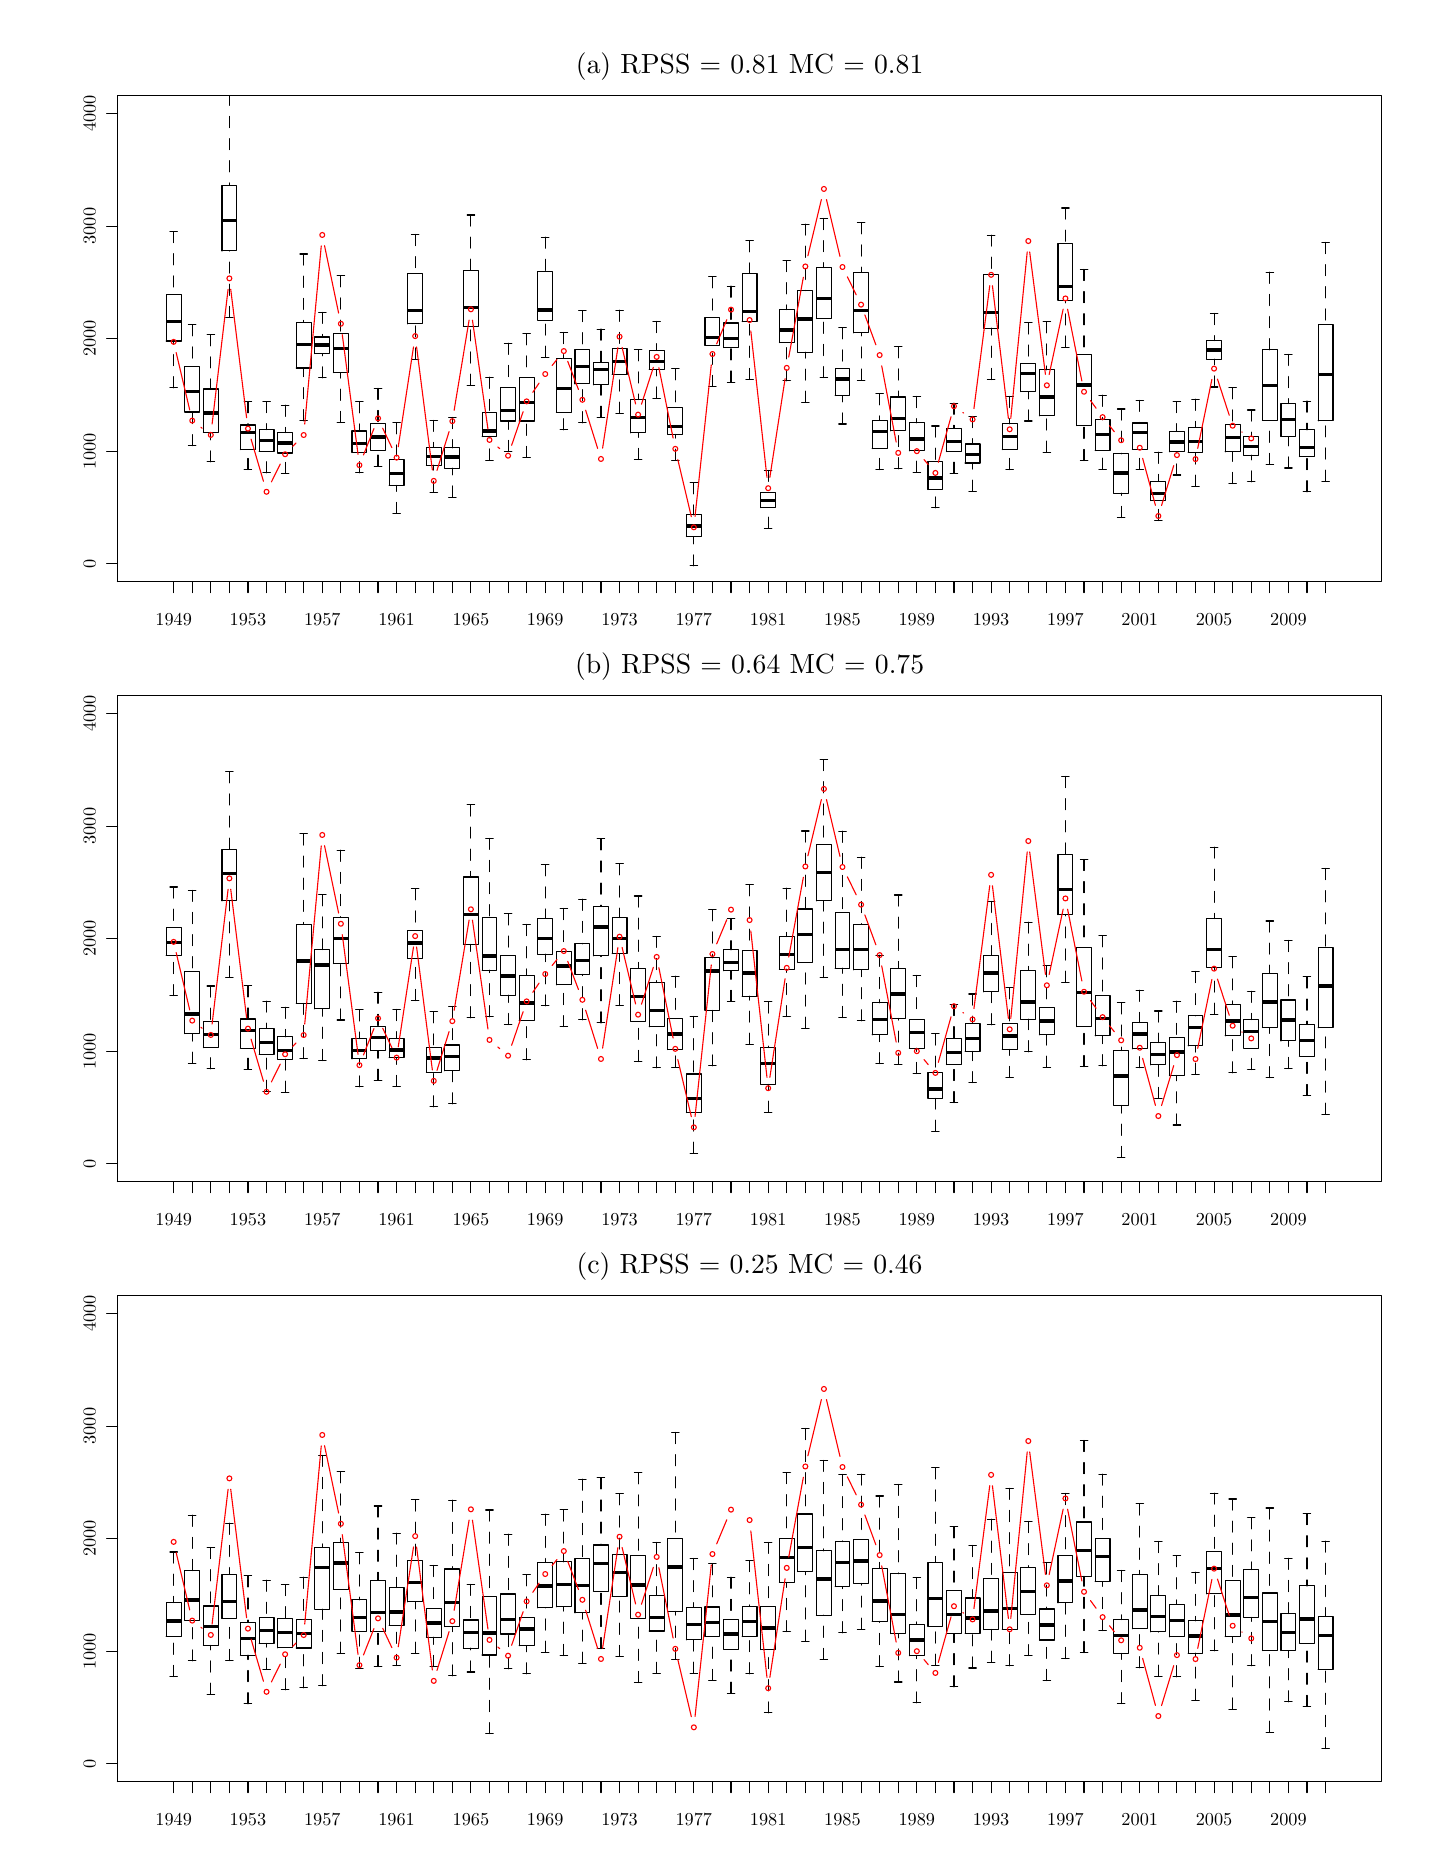
\begin{tikzpicture}[x=1pt,y=1pt]
\definecolor[named]{drawColor}{rgb}{0.00,0.00,0.00}
\definecolor[named]{fillColor}{rgb}{1.00,1.00,1.00}
\fill[color=fillColor,] (0,0) rectangle (505.89,650.43);
\begin{scope}
\path[clip] ( 32.47,450.25) rectangle (489.26,625.88);
\definecolor[named]{drawColor}{rgb}{0.00,0.00,0.00}

\draw[color=drawColor,line width= 1.2pt,line join=round,fill opacity=0.00,] ( 50.06,544.22) -- ( 55.43,544.22);

\draw[color=drawColor,dash pattern=on 4pt off 4pt ,line cap=round,line join=round,fill opacity=0.00,] ( 52.75,520.31) -- ( 52.75,537.21);

\draw[color=drawColor,dash pattern=on 4pt off 4pt ,line cap=round,line join=round,fill opacity=0.00,] ( 52.75,576.73) -- ( 52.75,553.85);

\draw[color=drawColor,line cap=round,line join=round,fill opacity=0.00,] ( 51.40,520.31) -- ( 54.09,520.31);

\draw[color=drawColor,line cap=round,line join=round,fill opacity=0.00,] ( 51.40,576.73) -- ( 54.09,576.73);

\draw[color=drawColor,line cap=round,line join=round,fill opacity=0.00,] ( 50.06,537.21) --
	( 55.43,537.21) --
	( 55.43,553.85) --
	( 50.06,553.85) --
	( 50.06,537.21);

\draw[color=drawColor,line width= 1.2pt,line join=round,fill opacity=0.00,] ( 56.77,518.86) -- ( 62.15,518.86);

\draw[color=drawColor,dash pattern=on 4pt off 4pt ,line cap=round,line join=round,fill opacity=0.00,] ( 59.46,499.37) -- ( 59.46,511.56);

\draw[color=drawColor,dash pattern=on 4pt off 4pt ,line cap=round,line join=round,fill opacity=0.00,] ( 59.46,543.03) -- ( 59.46,527.90);

\draw[color=drawColor,line cap=round,line join=round,fill opacity=0.00,] ( 58.12,499.37) -- ( 60.80,499.37);

\draw[color=drawColor,line cap=round,line join=round,fill opacity=0.00,] ( 58.12,543.03) -- ( 60.80,543.03);

\draw[color=drawColor,line cap=round,line join=round,fill opacity=0.00,] ( 56.77,511.56) --
	( 62.15,511.56) --
	( 62.15,527.90) --
	( 56.77,527.90) --
	( 56.77,511.56);

\draw[color=drawColor,line width= 1.2pt,line join=round,fill opacity=0.00,] ( 63.49,511.23) -- ( 68.86,511.23);

\draw[color=drawColor,dash pattern=on 4pt off 4pt ,line cap=round,line join=round,fill opacity=0.00,] ( 66.17,493.51) -- ( 66.17,504.20);

\draw[color=drawColor,dash pattern=on 4pt off 4pt ,line cap=round,line join=round,fill opacity=0.00,] ( 66.17,539.47) -- ( 66.17,519.86);

\draw[color=drawColor,line cap=round,line join=round,fill opacity=0.00,] ( 64.83,493.51) -- ( 67.52,493.51);

\draw[color=drawColor,line cap=round,line join=round,fill opacity=0.00,] ( 64.83,539.47) -- ( 67.52,539.47);

\draw[color=drawColor,line cap=round,line join=round,fill opacity=0.00,] ( 63.49,504.20) --
	( 68.86,504.20) --
	( 68.86,519.86) --
	( 63.49,519.86) --
	( 63.49,504.20);

\draw[color=drawColor,line width= 1.2pt,line join=round,fill opacity=0.00,] ( 70.20,580.70) -- ( 75.57,580.70);

\draw[color=drawColor,dash pattern=on 4pt off 4pt ,line cap=round,line join=round,fill opacity=0.00,] ( 72.89,545.73) -- ( 72.89,569.75);

\draw[color=drawColor,dash pattern=on 4pt off 4pt ,line cap=round,line join=round,fill opacity=0.00,] ( 72.89,626.34) -- ( 72.89,593.45);

\draw[color=drawColor,line cap=round,line join=round,fill opacity=0.00,] ( 71.54,545.73) -- ( 74.23,545.73);

\draw[color=drawColor,line cap=round,line join=round,fill opacity=0.00,] ( 71.54,626.34) -- ( 74.23,626.34);

\draw[color=drawColor,line cap=round,line join=round,fill opacity=0.00,] ( 70.20,569.75) --
	( 75.57,569.75) --
	( 75.57,593.45) --
	( 70.20,593.45) --
	( 70.20,569.75);

\draw[color=drawColor,line width= 1.2pt,line join=round,fill opacity=0.00,] ( 76.92,504.04) -- ( 82.29,504.04);

\draw[color=drawColor,dash pattern=on 4pt off 4pt ,line cap=round,line join=round,fill opacity=0.00,] ( 79.60,490.74) -- ( 79.60,497.95);

\draw[color=drawColor,dash pattern=on 4pt off 4pt ,line cap=round,line join=round,fill opacity=0.00,] ( 79.60,515.27) -- ( 79.60,506.83);

\draw[color=drawColor,line cap=round,line join=round,fill opacity=0.00,] ( 78.26,490.74) -- ( 80.94,490.74);

\draw[color=drawColor,line cap=round,line join=round,fill opacity=0.00,] ( 78.26,515.27) -- ( 80.94,515.27);

\draw[color=drawColor,line cap=round,line join=round,fill opacity=0.00,] ( 76.92,497.95) --
	( 82.29,497.95) --
	( 82.29,506.83) --
	( 76.92,506.83) --
	( 76.92,497.95);

\draw[color=drawColor,line width= 1.2pt,line join=round,fill opacity=0.00,] ( 83.63,501.16) -- ( 89.00,501.16);

\draw[color=drawColor,dash pattern=on 4pt off 4pt ,line cap=round,line join=round,fill opacity=0.00,] ( 86.31,489.56) -- ( 86.31,497.36);

\draw[color=drawColor,dash pattern=on 4pt off 4pt ,line cap=round,line join=round,fill opacity=0.00,] ( 86.31,515.30) -- ( 86.31,505.20);

\draw[color=drawColor,line cap=round,line join=round,fill opacity=0.00,] ( 84.97,489.56) -- ( 87.66,489.56);

\draw[color=drawColor,line cap=round,line join=round,fill opacity=0.00,] ( 84.97,515.30) -- ( 87.66,515.30);

\draw[color=drawColor,line cap=round,line join=round,fill opacity=0.00,] ( 83.63,497.36) --
	( 89.00,497.36) --
	( 89.00,505.20) --
	( 83.63,505.20) --
	( 83.63,497.36);

\draw[color=drawColor,line width= 1.2pt,line join=round,fill opacity=0.00,] ( 90.34,500.31) -- ( 95.71,500.31);

\draw[color=drawColor,dash pattern=on 4pt off 4pt ,line cap=round,line join=round,fill opacity=0.00,] ( 93.03,489.35) -- ( 93.03,496.73);

\draw[color=drawColor,dash pattern=on 4pt off 4pt ,line cap=round,line join=round,fill opacity=0.00,] ( 93.03,513.98) -- ( 93.03,504.15);

\draw[color=drawColor,line cap=round,line join=round,fill opacity=0.00,] ( 91.69,489.35) -- ( 94.37,489.35);

\draw[color=drawColor,line cap=round,line join=round,fill opacity=0.00,] ( 91.69,513.98) -- ( 94.37,513.98);

\draw[color=drawColor,line cap=round,line join=round,fill opacity=0.00,] ( 90.34,496.73) --
	( 95.71,496.73) --
	( 95.71,504.15) --
	( 90.34,504.15) --
	( 90.34,496.73);

\draw[color=drawColor,line width= 1.2pt,line join=round,fill opacity=0.00,] ( 97.06,535.95) -- (102.43,535.95);

\draw[color=drawColor,dash pattern=on 4pt off 4pt ,line cap=round,line join=round,fill opacity=0.00,] ( 99.74,508.37) -- ( 99.74,527.43);

\draw[color=drawColor,dash pattern=on 4pt off 4pt ,line cap=round,line join=round,fill opacity=0.00,] ( 99.74,568.63) -- ( 99.74,543.92);

\draw[color=drawColor,line cap=round,line join=round,fill opacity=0.00,] ( 98.40,508.37) -- (101.08,508.37);

\draw[color=drawColor,line cap=round,line join=round,fill opacity=0.00,] ( 98.40,568.63) -- (101.08,568.63);

\draw[color=drawColor,line cap=round,line join=round,fill opacity=0.00,] ( 97.06,527.43) --
	(102.43,527.43) --
	(102.43,543.92) --
	( 97.06,543.92) --
	( 97.06,527.43);

\draw[color=drawColor,line width= 1.2pt,line join=round,fill opacity=0.00,] (103.77,535.70) -- (109.14,535.70);

\draw[color=drawColor,dash pattern=on 4pt off 4pt ,line cap=round,line join=round,fill opacity=0.00,] (106.45,523.88) -- (106.45,532.65);

\draw[color=drawColor,dash pattern=on 4pt off 4pt ,line cap=round,line join=round,fill opacity=0.00,] (106.45,547.57) -- (106.45,538.63);

\draw[color=drawColor,line cap=round,line join=round,fill opacity=0.00,] (105.11,523.88) -- (107.80,523.88);

\draw[color=drawColor,line cap=round,line join=round,fill opacity=0.00,] (105.11,547.57) -- (107.80,547.57);

\draw[color=drawColor,line cap=round,line join=round,fill opacity=0.00,] (103.77,532.65) --
	(109.14,532.65) --
	(109.14,538.63) --
	(103.77,538.63) --
	(103.77,532.65);

\draw[color=drawColor,line width= 1.2pt,line join=round,fill opacity=0.00,] (110.48,534.42) -- (115.85,534.42);

\draw[color=drawColor,dash pattern=on 4pt off 4pt ,line cap=round,line join=round,fill opacity=0.00,] (113.17,507.77) -- (113.17,525.75);

\draw[color=drawColor,dash pattern=on 4pt off 4pt ,line cap=round,line join=round,fill opacity=0.00,] (113.17,560.76) -- (113.17,539.82);

\draw[color=drawColor,line cap=round,line join=round,fill opacity=0.00,] (111.83,507.77) -- (114.51,507.77);

\draw[color=drawColor,line cap=round,line join=round,fill opacity=0.00,] (111.83,560.76) -- (114.51,560.76);

\draw[color=drawColor,line cap=round,line join=round,fill opacity=0.00,] (110.48,525.75) --
	(115.85,525.75) --
	(115.85,539.82) --
	(110.48,539.82) --
	(110.48,525.75);

\draw[color=drawColor,line width= 1.2pt,line join=round,fill opacity=0.00,] (117.20,500.10) -- (122.57,500.10);

\draw[color=drawColor,dash pattern=on 4pt off 4pt ,line cap=round,line join=round,fill opacity=0.00,] (119.88,489.60) -- (119.88,496.93);

\draw[color=drawColor,dash pattern=on 4pt off 4pt ,line cap=round,line join=round,fill opacity=0.00,] (119.88,515.24) -- (119.88,504.67);

\draw[color=drawColor,line cap=round,line join=round,fill opacity=0.00,] (118.54,489.60) -- (121.22,489.60);

\draw[color=drawColor,line cap=round,line join=round,fill opacity=0.00,] (118.54,515.24) -- (121.22,515.24);

\draw[color=drawColor,line cap=round,line join=round,fill opacity=0.00,] (117.20,496.93) --
	(122.57,496.93) --
	(122.57,504.67) --
	(117.20,504.67) --
	(117.20,496.93);

\draw[color=drawColor,line width= 1.2pt,line join=round,fill opacity=0.00,] (123.91,502.51) -- (129.28,502.51);

\draw[color=drawColor,dash pattern=on 4pt off 4pt ,line cap=round,line join=round,fill opacity=0.00,] (126.60,491.99) -- (126.60,497.78);

\draw[color=drawColor,dash pattern=on 4pt off 4pt ,line cap=round,line join=round,fill opacity=0.00,] (126.60,520.09) -- (126.60,507.39);

\draw[color=drawColor,line cap=round,line join=round,fill opacity=0.00,] (125.25,491.99) -- (127.94,491.99);

\draw[color=drawColor,line cap=round,line join=round,fill opacity=0.00,] (125.25,520.09) -- (127.94,520.09);

\draw[color=drawColor,line cap=round,line join=round,fill opacity=0.00,] (123.91,497.78) --
	(129.28,497.78) --
	(129.28,507.39) --
	(123.91,507.39) --
	(123.91,497.78);

\draw[color=drawColor,line width= 1.2pt,line join=round,fill opacity=0.00,] (130.62,489.34) -- (135.99,489.34);

\draw[color=drawColor,dash pattern=on 4pt off 4pt ,line cap=round,line join=round,fill opacity=0.00,] (133.31,474.91) -- (133.31,485.03);

\draw[color=drawColor,dash pattern=on 4pt off 4pt ,line cap=round,line join=round,fill opacity=0.00,] (133.31,507.65) -- (133.31,494.24);

\draw[color=drawColor,line cap=round,line join=round,fill opacity=0.00,] (131.97,474.91) -- (134.65,474.91);

\draw[color=drawColor,line cap=round,line join=round,fill opacity=0.00,] (131.97,507.65) -- (134.65,507.65);

\draw[color=drawColor,line cap=round,line join=round,fill opacity=0.00,] (130.62,485.03) --
	(135.99,485.03) --
	(135.99,494.24) --
	(130.62,494.24) --
	(130.62,485.03);

\draw[color=drawColor,line width= 1.2pt,line join=round,fill opacity=0.00,] (137.34,548.18) -- (142.71,548.18);

\draw[color=drawColor,dash pattern=on 4pt off 4pt ,line cap=round,line join=round,fill opacity=0.00,] (140.02,530.67) -- (140.02,543.42);

\draw[color=drawColor,dash pattern=on 4pt off 4pt ,line cap=round,line join=round,fill opacity=0.00,] (140.02,575.71) -- (140.02,561.74);

\draw[color=drawColor,line cap=round,line join=round,fill opacity=0.00,] (138.68,530.67) -- (141.36,530.67);

\draw[color=drawColor,line cap=round,line join=round,fill opacity=0.00,] (138.68,575.71) -- (141.36,575.71);

\draw[color=drawColor,line cap=round,line join=round,fill opacity=0.00,] (137.34,543.42) --
	(142.71,543.42) --
	(142.71,561.74) --
	(137.34,561.74) --
	(137.34,543.42);

\draw[color=drawColor,line width= 1.2pt,line join=round,fill opacity=0.00,] (144.05,495.54) -- (149.42,495.54);

\draw[color=drawColor,dash pattern=on 4pt off 4pt ,line cap=round,line join=round,fill opacity=0.00,] (146.74,482.56) -- (146.74,492.33);

\draw[color=drawColor,dash pattern=on 4pt off 4pt ,line cap=round,line join=round,fill opacity=0.00,] (146.74,508.52) -- (146.74,498.86);

\draw[color=drawColor,line cap=round,line join=round,fill opacity=0.00,] (145.39,482.56) -- (148.08,482.56);

\draw[color=drawColor,line cap=round,line join=round,fill opacity=0.00,] (145.39,508.52) -- (148.08,508.52);

\draw[color=drawColor,line cap=round,line join=round,fill opacity=0.00,] (144.05,492.33) --
	(149.42,492.33) --
	(149.42,498.86) --
	(144.05,498.86) --
	(144.05,492.33);

\draw[color=drawColor,line width= 1.2pt,line join=round,fill opacity=0.00,] (150.76,495.30) -- (156.13,495.30);

\draw[color=drawColor,dash pattern=on 4pt off 4pt ,line cap=round,line join=round,fill opacity=0.00,] (153.45,480.81) -- (153.45,491.22);

\draw[color=drawColor,dash pattern=on 4pt off 4pt ,line cap=round,line join=round,fill opacity=0.00,] (153.45,509.56) -- (153.45,498.58);

\draw[color=drawColor,line cap=round,line join=round,fill opacity=0.00,] (152.11,480.81) -- (154.79,480.81);

\draw[color=drawColor,line cap=round,line join=round,fill opacity=0.00,] (152.11,509.56) -- (154.79,509.56);

\draw[color=drawColor,line cap=round,line join=round,fill opacity=0.00,] (150.76,491.22) --
	(156.13,491.22) --
	(156.13,498.58) --
	(150.76,498.58) --
	(150.76,491.22);

\draw[color=drawColor,line width= 1.2pt,line join=round,fill opacity=0.00,] (157.48,549.40) -- (162.85,549.40);

\draw[color=drawColor,dash pattern=on 4pt off 4pt ,line cap=round,line join=round,fill opacity=0.00,] (160.16,521.24) -- (160.16,542.59);

\draw[color=drawColor,dash pattern=on 4pt off 4pt ,line cap=round,line join=round,fill opacity=0.00,] (160.16,582.75) -- (160.16,562.67);

\draw[color=drawColor,line cap=round,line join=round,fill opacity=0.00,] (158.82,521.24) -- (161.51,521.24);

\draw[color=drawColor,line cap=round,line join=round,fill opacity=0.00,] (158.82,582.75) -- (161.51,582.75);

\draw[color=drawColor,line cap=round,line join=round,fill opacity=0.00,] (157.48,542.59) --
	(162.85,542.59) --
	(162.85,562.67) --
	(157.48,562.67) --
	(157.48,542.59);

\draw[color=drawColor,line width= 1.2pt,line join=round,fill opacity=0.00,] (164.19,504.65) -- (169.56,504.65);

\draw[color=drawColor,dash pattern=on 4pt off 4pt ,line cap=round,line join=round,fill opacity=0.00,] (166.88,494.18) -- (166.88,502.69);

\draw[color=drawColor,dash pattern=on 4pt off 4pt ,line cap=round,line join=round,fill opacity=0.00,] (166.88,524.11) -- (166.88,511.41);

\draw[color=drawColor,line cap=round,line join=round,fill opacity=0.00,] (165.53,494.18) -- (168.22,494.18);

\draw[color=drawColor,line cap=round,line join=round,fill opacity=0.00,] (165.53,524.11) -- (168.22,524.11);

\draw[color=drawColor,line cap=round,line join=round,fill opacity=0.00,] (164.19,502.69) --
	(169.56,502.69) --
	(169.56,511.41) --
	(164.19,511.41) --
	(164.19,502.69);

\draw[color=drawColor,line width= 1.2pt,line join=round,fill opacity=0.00,] (170.90,512.10) -- (176.28,512.10);

\draw[color=drawColor,dash pattern=on 4pt off 4pt ,line cap=round,line join=round,fill opacity=0.00,] (173.59,497.27) -- (173.59,508.29);

\draw[color=drawColor,dash pattern=on 4pt off 4pt ,line cap=round,line join=round,fill opacity=0.00,] (173.59,536.38) -- (173.59,520.50);

\draw[color=drawColor,line cap=round,line join=round,fill opacity=0.00,] (172.25,497.27) -- (174.93,497.27);

\draw[color=drawColor,line cap=round,line join=round,fill opacity=0.00,] (172.25,536.38) -- (174.93,536.38);

\draw[color=drawColor,line cap=round,line join=round,fill opacity=0.00,] (170.90,508.29) --
	(176.28,508.29) --
	(176.28,520.50) --
	(170.90,520.50) --
	(170.90,508.29);

\draw[color=drawColor,line width= 1.2pt,line join=round,fill opacity=0.00,] (177.62,515.00) -- (182.99,515.00);

\draw[color=drawColor,dash pattern=on 4pt off 4pt ,line cap=round,line join=round,fill opacity=0.00,] (180.30,495.15) -- (180.30,508.31);

\draw[color=drawColor,dash pattern=on 4pt off 4pt ,line cap=round,line join=round,fill opacity=0.00,] (180.30,539.84) -- (180.30,524.06);

\draw[color=drawColor,line cap=round,line join=round,fill opacity=0.00,] (178.96,495.15) -- (181.65,495.15);

\draw[color=drawColor,line cap=round,line join=round,fill opacity=0.00,] (178.96,539.84) -- (181.65,539.84);

\draw[color=drawColor,line cap=round,line join=round,fill opacity=0.00,] (177.62,508.31) --
	(182.99,508.31) --
	(182.99,524.06) --
	(177.62,524.06) --
	(177.62,508.31);

\draw[color=drawColor,line width= 1.2pt,line join=round,fill opacity=0.00,] (184.33,548.35) -- (189.70,548.35);

\draw[color=drawColor,dash pattern=on 4pt off 4pt ,line cap=round,line join=round,fill opacity=0.00,] (187.02,531.31) -- (187.02,544.72);

\draw[color=drawColor,dash pattern=on 4pt off 4pt ,line cap=round,line join=round,fill opacity=0.00,] (187.02,574.73) -- (187.02,562.18);

\draw[color=drawColor,line cap=round,line join=round,fill opacity=0.00,] (185.67,531.31) -- (188.36,531.31);

\draw[color=drawColor,line cap=round,line join=round,fill opacity=0.00,] (185.67,574.73) -- (188.36,574.73);

\draw[color=drawColor,line cap=round,line join=round,fill opacity=0.00,] (184.33,544.72) --
	(189.70,544.72) --
	(189.70,562.18) --
	(184.33,562.18) --
	(184.33,544.72);

\draw[color=drawColor,line width= 1.2pt,line join=round,fill opacity=0.00,] (191.04,520.01) -- (196.42,520.01);

\draw[color=drawColor,dash pattern=on 4pt off 4pt ,line cap=round,line join=round,fill opacity=0.00,] (193.73,505.10) -- (193.73,511.52);

\draw[color=drawColor,dash pattern=on 4pt off 4pt ,line cap=round,line join=round,fill opacity=0.00,] (193.73,540.26) -- (193.73,530.99);

\draw[color=drawColor,line cap=round,line join=round,fill opacity=0.00,] (192.39,505.10) -- (195.07,505.10);

\draw[color=drawColor,line cap=round,line join=round,fill opacity=0.00,] (192.39,540.26) -- (195.07,540.26);

\draw[color=drawColor,line cap=round,line join=round,fill opacity=0.00,] (191.04,511.52) --
	(196.42,511.52) --
	(196.42,530.99) --
	(191.04,530.99) --
	(191.04,511.52);

\draw[color=drawColor,line width= 1.2pt,line join=round,fill opacity=0.00,] (197.76,528.02) -- (203.13,528.02);

\draw[color=drawColor,dash pattern=on 4pt off 4pt ,line cap=round,line join=round,fill opacity=0.00,] (200.44,507.64) -- (200.44,521.69);

\draw[color=drawColor,dash pattern=on 4pt off 4pt ,line cap=round,line join=round,fill opacity=0.00,] (200.44,548.18) -- (200.44,534.27);

\draw[color=drawColor,line cap=round,line join=round,fill opacity=0.00,] (199.10,507.64) -- (201.79,507.64);

\draw[color=drawColor,line cap=round,line join=round,fill opacity=0.00,] (199.10,548.18) -- (201.79,548.18);

\draw[color=drawColor,line cap=round,line join=round,fill opacity=0.00,] (197.76,521.69) --
	(203.13,521.69) --
	(203.13,534.27) --
	(197.76,534.27) --
	(197.76,521.69);

\draw[color=drawColor,line width= 1.2pt,line join=round,fill opacity=0.00,] (204.47,526.86) -- (209.84,526.86);

\draw[color=drawColor,dash pattern=on 4pt off 4pt ,line cap=round,line join=round,fill opacity=0.00,] (207.16,509.63) -- (207.16,521.36);

\draw[color=drawColor,dash pattern=on 4pt off 4pt ,line cap=round,line join=round,fill opacity=0.00,] (207.16,541.51) -- (207.16,529.42);

\draw[color=drawColor,line cap=round,line join=round,fill opacity=0.00,] (205.81,509.63) -- (208.50,509.63);

\draw[color=drawColor,line cap=round,line join=round,fill opacity=0.00,] (205.81,541.51) -- (208.50,541.51);

\draw[color=drawColor,line cap=round,line join=round,fill opacity=0.00,] (204.47,521.36) --
	(209.84,521.36) --
	(209.84,529.42) --
	(204.47,529.42) --
	(204.47,521.36);

\draw[color=drawColor,line width= 1.2pt,line join=round,fill opacity=0.00,] (211.19,529.71) -- (216.56,529.71);

\draw[color=drawColor,dash pattern=on 4pt off 4pt ,line cap=round,line join=round,fill opacity=0.00,] (213.87,511.11) -- (213.87,525.18);

\draw[color=drawColor,dash pattern=on 4pt off 4pt ,line cap=round,line join=round,fill opacity=0.00,] (213.87,548.34) -- (213.87,534.57);

\draw[color=drawColor,line cap=round,line join=round,fill opacity=0.00,] (212.53,511.11) -- (215.21,511.11);

\draw[color=drawColor,line cap=round,line join=round,fill opacity=0.00,] (212.53,548.34) -- (215.21,548.34);

\draw[color=drawColor,line cap=round,line join=round,fill opacity=0.00,] (211.19,525.18) --
	(216.56,525.18) --
	(216.56,534.57) --
	(211.19,534.57) --
	(211.19,525.18);

\draw[color=drawColor,line width= 1.2pt,line join=round,fill opacity=0.00,] (217.90,509.57) -- (223.27,509.57);

\draw[color=drawColor,dash pattern=on 4pt off 4pt ,line cap=round,line join=round,fill opacity=0.00,] (220.58,494.40) -- (220.58,503.99);

\draw[color=drawColor,dash pattern=on 4pt off 4pt ,line cap=round,line join=round,fill opacity=0.00,] (220.58,534.04) -- (220.58,516.02);

\draw[color=drawColor,line cap=round,line join=round,fill opacity=0.00,] (219.24,494.40) -- (221.93,494.40);

\draw[color=drawColor,line cap=round,line join=round,fill opacity=0.00,] (219.24,534.04) -- (221.93,534.04);

\draw[color=drawColor,line cap=round,line join=round,fill opacity=0.00,] (217.90,503.99) --
	(223.27,503.99) --
	(223.27,516.02) --
	(217.90,516.02) --
	(217.90,503.99);

\draw[color=drawColor,line width= 1.2pt,line join=round,fill opacity=0.00,] (224.61,529.72) -- (229.98,529.72);

\draw[color=drawColor,dash pattern=on 4pt off 4pt ,line cap=round,line join=round,fill opacity=0.00,] (227.30,516.58) -- (227.30,526.96);

\draw[color=drawColor,dash pattern=on 4pt off 4pt ,line cap=round,line join=round,fill opacity=0.00,] (227.30,544.24) -- (227.30,533.93);

\draw[color=drawColor,line cap=round,line join=round,fill opacity=0.00,] (225.95,516.58) -- (228.64,516.58);

\draw[color=drawColor,line cap=round,line join=round,fill opacity=0.00,] (225.95,544.24) -- (228.64,544.24);

\draw[color=drawColor,line cap=round,line join=round,fill opacity=0.00,] (224.61,526.96) --
	(229.98,526.96) --
	(229.98,533.93) --
	(224.61,533.93) --
	(224.61,526.96);

\draw[color=drawColor,line width= 1.2pt,line join=round,fill opacity=0.00,] (231.33,506.38) -- (236.70,506.38);

\draw[color=drawColor,dash pattern=on 4pt off 4pt ,line cap=round,line join=round,fill opacity=0.00,] (234.01,494.09) -- (234.01,503.44);

\draw[color=drawColor,dash pattern=on 4pt off 4pt ,line cap=round,line join=round,fill opacity=0.00,] (234.01,527.20) -- (234.01,513.22);

\draw[color=drawColor,line cap=round,line join=round,fill opacity=0.00,] (232.67,494.09) -- (235.35,494.09);

\draw[color=drawColor,line cap=round,line join=round,fill opacity=0.00,] (232.67,527.20) -- (235.35,527.20);

\draw[color=drawColor,line cap=round,line join=round,fill opacity=0.00,] (231.33,503.44) --
	(236.70,503.44) --
	(236.70,513.22) --
	(231.33,513.22) --
	(231.33,503.44);

\draw[color=drawColor,line width= 1.2pt,line join=round,fill opacity=0.00,] (238.04,470.40) -- (243.41,470.40);

\draw[color=drawColor,dash pattern=on 4pt off 4pt ,line cap=round,line join=round,fill opacity=0.00,] (240.72,455.93) -- (240.72,466.53);

\draw[color=drawColor,dash pattern=on 4pt off 4pt ,line cap=round,line join=round,fill opacity=0.00,] (240.72,486.01) -- (240.72,474.35);

\draw[color=drawColor,line cap=round,line join=round,fill opacity=0.00,] (239.38,455.93) -- (242.07,455.93);

\draw[color=drawColor,line cap=round,line join=round,fill opacity=0.00,] (239.38,486.01) -- (242.07,486.01);

\draw[color=drawColor,line cap=round,line join=round,fill opacity=0.00,] (238.04,466.53) --
	(243.41,466.53) --
	(243.41,474.35) --
	(238.04,474.35) --
	(238.04,466.53);

\draw[color=drawColor,line width= 1.2pt,line join=round,fill opacity=0.00,] (244.75,538.56) -- (250.12,538.56);

\draw[color=drawColor,dash pattern=on 4pt off 4pt ,line cap=round,line join=round,fill opacity=0.00,] (247.44,520.78) -- (247.44,535.60);

\draw[color=drawColor,dash pattern=on 4pt off 4pt ,line cap=round,line join=round,fill opacity=0.00,] (247.44,560.40) -- (247.44,545.57);

\draw[color=drawColor,line cap=round,line join=round,fill opacity=0.00,] (246.10,520.78) -- (248.78,520.78);

\draw[color=drawColor,line cap=round,line join=round,fill opacity=0.00,] (246.10,560.40) -- (248.78,560.40);

\draw[color=drawColor,line cap=round,line join=round,fill opacity=0.00,] (244.75,535.60) --
	(250.12,535.60) --
	(250.12,545.57) --
	(244.75,545.57) --
	(244.75,535.60);

\draw[color=drawColor,line width= 1.2pt,line join=round,fill opacity=0.00,] (251.47,538.03) -- (256.84,538.03);

\draw[color=drawColor,dash pattern=on 4pt off 4pt ,line cap=round,line join=round,fill opacity=0.00,] (254.15,522.36) -- (254.15,534.84);

\draw[color=drawColor,dash pattern=on 4pt off 4pt ,line cap=round,line join=round,fill opacity=0.00,] (254.15,557.02) -- (254.15,543.72);

\draw[color=drawColor,line cap=round,line join=round,fill opacity=0.00,] (252.81,522.36) -- (255.49,522.36);

\draw[color=drawColor,line cap=round,line join=round,fill opacity=0.00,] (252.81,557.02) -- (255.49,557.02);

\draw[color=drawColor,line cap=round,line join=round,fill opacity=0.00,] (251.47,534.84) --
	(256.84,534.84) --
	(256.84,543.72) --
	(251.47,543.72) --
	(251.47,534.84);

\draw[color=drawColor,line width= 1.2pt,line join=round,fill opacity=0.00,] (258.18,547.83) -- (263.55,547.83);

\draw[color=drawColor,dash pattern=on 4pt off 4pt ,line cap=round,line join=round,fill opacity=0.00,] (260.87,523.32) -- (260.87,544.19);

\draw[color=drawColor,dash pattern=on 4pt off 4pt ,line cap=round,line join=round,fill opacity=0.00,] (260.87,573.45) -- (260.87,561.69);

\draw[color=drawColor,line cap=round,line join=round,fill opacity=0.00,] (259.52,523.32) -- (262.21,523.32);

\draw[color=drawColor,line cap=round,line join=round,fill opacity=0.00,] (259.52,573.45) -- (262.21,573.45);

\draw[color=drawColor,line cap=round,line join=round,fill opacity=0.00,] (258.18,544.19) --
	(263.55,544.19) --
	(263.55,561.69) --
	(258.18,561.69) --
	(258.18,544.19);

\draw[color=drawColor,line width= 1.2pt,line join=round,fill opacity=0.00,] (264.89,479.52) -- (270.26,479.52);

\draw[color=drawColor,dash pattern=on 4pt off 4pt ,line cap=round,line join=round,fill opacity=0.00,] (267.58,469.52) -- (267.58,477.02);

\draw[color=drawColor,dash pattern=on 4pt off 4pt ,line cap=round,line join=round,fill opacity=0.00,] (267.58,490.46) -- (267.58,482.50);

\draw[color=drawColor,line cap=round,line join=round,fill opacity=0.00,] (266.24,469.52) -- (268.92,469.52);

\draw[color=drawColor,line cap=round,line join=round,fill opacity=0.00,] (266.24,490.46) -- (268.92,490.46);

\draw[color=drawColor,line cap=round,line join=round,fill opacity=0.00,] (264.89,477.02) --
	(270.26,477.02) --
	(270.26,482.50) --
	(264.89,482.50) --
	(264.89,477.02);

\draw[color=drawColor,line width= 1.2pt,line join=round,fill opacity=0.00,] (271.61,541.13) -- (276.98,541.13);

\draw[color=drawColor,dash pattern=on 4pt off 4pt ,line cap=round,line join=round,fill opacity=0.00,] (274.29,522.79) -- (274.29,536.61);

\draw[color=drawColor,dash pattern=on 4pt off 4pt ,line cap=round,line join=round,fill opacity=0.00,] (274.29,566.27) -- (274.29,548.57);

\draw[color=drawColor,line cap=round,line join=round,fill opacity=0.00,] (272.95,522.79) -- (275.63,522.79);

\draw[color=drawColor,line cap=round,line join=round,fill opacity=0.00,] (272.95,566.27) -- (275.63,566.27);

\draw[color=drawColor,line cap=round,line join=round,fill opacity=0.00,] (271.61,536.61) --
	(276.98,536.61) --
	(276.98,548.57) --
	(271.61,548.57) --
	(271.61,536.61);

\draw[color=drawColor,line width= 1.2pt,line join=round,fill opacity=0.00,] (278.32,545.18) -- (283.69,545.18);

\draw[color=drawColor,dash pattern=on 4pt off 4pt ,line cap=round,line join=round,fill opacity=0.00,] (281.01,515.04) -- (281.01,533.13);

\draw[color=drawColor,dash pattern=on 4pt off 4pt ,line cap=round,line join=round,fill opacity=0.00,] (281.01,579.44) -- (281.01,555.44);

\draw[color=drawColor,line cap=round,line join=round,fill opacity=0.00,] (279.66,515.04) -- (282.35,515.04);

\draw[color=drawColor,line cap=round,line join=round,fill opacity=0.00,] (279.66,579.44) -- (282.35,579.44);

\draw[color=drawColor,line cap=round,line join=round,fill opacity=0.00,] (278.32,533.13) --
	(283.69,533.13) --
	(283.69,555.44) --
	(278.32,555.44) --
	(278.32,533.13);

\draw[color=drawColor,line width= 1.2pt,line join=round,fill opacity=0.00,] (285.03,552.63) -- (290.40,552.63);

\draw[color=drawColor,dash pattern=on 4pt off 4pt ,line cap=round,line join=round,fill opacity=0.00,] (287.72,523.97) -- (287.72,545.34);

\draw[color=drawColor,dash pattern=on 4pt off 4pt ,line cap=round,line join=round,fill opacity=0.00,] (287.72,581.49) -- (287.72,563.71);

\draw[color=drawColor,line cap=round,line join=round,fill opacity=0.00,] (286.38,523.97) -- (289.06,523.97);

\draw[color=drawColor,line cap=round,line join=round,fill opacity=0.00,] (286.38,581.49) -- (289.06,581.49);

\draw[color=drawColor,line cap=round,line join=round,fill opacity=0.00,] (285.03,545.34) --
	(290.40,545.34) --
	(290.40,563.71) --
	(285.03,563.71) --
	(285.03,545.34);

\draw[color=drawColor,line width= 1.2pt,line join=round,fill opacity=0.00,] (291.75,523.49) -- (297.12,523.49);

\draw[color=drawColor,dash pattern=on 4pt off 4pt ,line cap=round,line join=round,fill opacity=0.00,] (294.43,507.21) -- (294.43,517.45);

\draw[color=drawColor,dash pattern=on 4pt off 4pt ,line cap=round,line join=round,fill opacity=0.00,] (294.43,541.95) -- (294.43,527.27);

\draw[color=drawColor,line cap=round,line join=round,fill opacity=0.00,] (293.09,507.21) -- (295.78,507.21);

\draw[color=drawColor,line cap=round,line join=round,fill opacity=0.00,] (293.09,541.95) -- (295.78,541.95);

\draw[color=drawColor,line cap=round,line join=round,fill opacity=0.00,] (291.75,517.45) --
	(297.12,517.45) --
	(297.12,527.27) --
	(291.75,527.27) --
	(291.75,517.45);

\draw[color=drawColor,line width= 1.2pt,line join=round,fill opacity=0.00,] (298.46,548.29) -- (303.83,548.29);

\draw[color=drawColor,dash pattern=on 4pt off 4pt ,line cap=round,line join=round,fill opacity=0.00,] (301.15,523.07) -- (301.15,540.12);

\draw[color=drawColor,dash pattern=on 4pt off 4pt ,line cap=round,line join=round,fill opacity=0.00,] (301.15,579.92) -- (301.15,562.00);

\draw[color=drawColor,line cap=round,line join=round,fill opacity=0.00,] (299.80,523.07) -- (302.49,523.07);

\draw[color=drawColor,line cap=round,line join=round,fill opacity=0.00,] (299.80,579.92) -- (302.49,579.92);

\draw[color=drawColor,line cap=round,line join=round,fill opacity=0.00,] (298.46,540.12) --
	(303.83,540.12) --
	(303.83,562.00) --
	(298.46,562.00) --
	(298.46,540.12);

\draw[color=drawColor,line width= 1.2pt,line join=round,fill opacity=0.00,] (305.17,504.45) -- (310.54,504.45);

\draw[color=drawColor,dash pattern=on 4pt off 4pt ,line cap=round,line join=round,fill opacity=0.00,] (307.86,490.76) -- (307.86,498.32);

\draw[color=drawColor,dash pattern=on 4pt off 4pt ,line cap=round,line join=round,fill opacity=0.00,] (307.86,518.13) -- (307.86,508.50);

\draw[color=drawColor,line cap=round,line join=round,fill opacity=0.00,] (306.52,490.76) -- (309.20,490.76);

\draw[color=drawColor,line cap=round,line join=round,fill opacity=0.00,] (306.52,518.13) -- (309.20,518.13);

\draw[color=drawColor,line cap=round,line join=round,fill opacity=0.00,] (305.17,498.32) --
	(310.54,498.32) --
	(310.54,508.50) --
	(305.17,508.50) --
	(305.17,498.32);

\draw[color=drawColor,line width= 1.2pt,line join=round,fill opacity=0.00,] (311.89,509.27) -- (317.26,509.27);

\draw[color=drawColor,dash pattern=on 4pt off 4pt ,line cap=round,line join=round,fill opacity=0.00,] (314.57,491.02) -- (314.57,504.75);

\draw[color=drawColor,dash pattern=on 4pt off 4pt ,line cap=round,line join=round,fill opacity=0.00,] (314.57,535.12) -- (314.57,516.98);

\draw[color=drawColor,line cap=round,line join=round,fill opacity=0.00,] (313.23,491.02) -- (315.92,491.02);

\draw[color=drawColor,line cap=round,line join=round,fill opacity=0.00,] (313.23,535.12) -- (315.92,535.12);

\draw[color=drawColor,line cap=round,line join=round,fill opacity=0.00,] (311.89,504.75) --
	(317.26,504.75) --
	(317.26,516.98) --
	(311.89,516.98) --
	(311.89,504.75);

\draw[color=drawColor,line width= 1.2pt,line join=round,fill opacity=0.00,] (318.60,501.77) -- (323.97,501.77);

\draw[color=drawColor,dash pattern=on 4pt off 4pt ,line cap=round,line join=round,fill opacity=0.00,] (321.29,489.81) -- (321.29,497.49);

\draw[color=drawColor,dash pattern=on 4pt off 4pt ,line cap=round,line join=round,fill opacity=0.00,] (321.29,517.16) -- (321.29,507.65);

\draw[color=drawColor,line cap=round,line join=round,fill opacity=0.00,] (319.94,489.81) -- (322.63,489.81);

\draw[color=drawColor,line cap=round,line join=round,fill opacity=0.00,] (319.94,517.16) -- (322.63,517.16);

\draw[color=drawColor,line cap=round,line join=round,fill opacity=0.00,] (318.60,497.49) --
	(323.97,497.49) --
	(323.97,507.65) --
	(318.60,507.65) --
	(318.60,497.49);

\draw[color=drawColor,line width= 1.2pt,line join=round,fill opacity=0.00,] (325.31,487.71) -- (330.69,487.71);

\draw[color=drawColor,dash pattern=on 4pt off 4pt ,line cap=round,line join=round,fill opacity=0.00,] (328.00,476.88) -- (328.00,483.52);

\draw[color=drawColor,dash pattern=on 4pt off 4pt ,line cap=round,line join=round,fill opacity=0.00,] (328.00,506.47) -- (328.00,493.68);

\draw[color=drawColor,line cap=round,line join=round,fill opacity=0.00,] (326.66,476.88) -- (329.34,476.88);

\draw[color=drawColor,line cap=round,line join=round,fill opacity=0.00,] (326.66,506.47) -- (329.34,506.47);

\draw[color=drawColor,line cap=round,line join=round,fill opacity=0.00,] (325.31,483.52) --
	(330.69,483.52) --
	(330.69,493.68) --
	(325.31,493.68) --
	(325.31,483.52);

\draw[color=drawColor,line width= 1.2pt,line join=round,fill opacity=0.00,] (332.03,500.84) -- (337.40,500.84);

\draw[color=drawColor,dash pattern=on 4pt off 4pt ,line cap=round,line join=round,fill opacity=0.00,] (334.71,489.39) -- (334.71,497.22);

\draw[color=drawColor,dash pattern=on 4pt off 4pt ,line cap=round,line join=round,fill opacity=0.00,] (334.71,514.74) -- (334.71,505.61);

\draw[color=drawColor,line cap=round,line join=round,fill opacity=0.00,] (333.37,489.39) -- (336.06,489.39);

\draw[color=drawColor,line cap=round,line join=round,fill opacity=0.00,] (333.37,514.74) -- (336.06,514.74);

\draw[color=drawColor,line cap=round,line join=round,fill opacity=0.00,] (332.03,497.22) --
	(337.40,497.22) --
	(337.40,505.61) --
	(332.03,505.61) --
	(332.03,497.22);

\draw[color=drawColor,line width= 1.2pt,line join=round,fill opacity=0.00,] (338.74,496.07) -- (344.11,496.07);

\draw[color=drawColor,dash pattern=on 4pt off 4pt ,line cap=round,line join=round,fill opacity=0.00,] (341.43,482.88) -- (341.43,493.11);

\draw[color=drawColor,dash pattern=on 4pt off 4pt ,line cap=round,line join=round,fill opacity=0.00,] (341.43,509.94) -- (341.43,499.98);

\draw[color=drawColor,line cap=round,line join=round,fill opacity=0.00,] (340.08,482.88) -- (342.77,482.88);

\draw[color=drawColor,line cap=round,line join=round,fill opacity=0.00,] (340.08,509.94) -- (342.77,509.94);

\draw[color=drawColor,line cap=round,line join=round,fill opacity=0.00,] (338.74,493.11) --
	(344.11,493.11) --
	(344.11,499.98) --
	(338.74,499.98) --
	(338.74,493.11);

\draw[color=drawColor,line width= 1.2pt,line join=round,fill opacity=0.00,] (345.45,547.48) -- (350.83,547.48);

\draw[color=drawColor,dash pattern=on 4pt off 4pt ,line cap=round,line join=round,fill opacity=0.00,] (348.14,523.30) -- (348.14,541.82);

\draw[color=drawColor,dash pattern=on 4pt off 4pt ,line cap=round,line join=round,fill opacity=0.00,] (348.14,575.47) -- (348.14,561.25);

\draw[color=drawColor,line cap=round,line join=round,fill opacity=0.00,] (346.80,523.30) -- (349.48,523.30);

\draw[color=drawColor,line cap=round,line join=round,fill opacity=0.00,] (346.80,575.47) -- (349.48,575.47);

\draw[color=drawColor,line cap=round,line join=round,fill opacity=0.00,] (345.45,541.82) --
	(350.83,541.82) --
	(350.83,561.25) --
	(345.45,561.25) --
	(345.45,541.82);

\draw[color=drawColor,line width= 1.2pt,line join=round,fill opacity=0.00,] (352.17,502.77) -- (357.54,502.77);

\draw[color=drawColor,dash pattern=on 4pt off 4pt ,line cap=round,line join=round,fill opacity=0.00,] (354.85,490.75) -- (354.85,497.93);

\draw[color=drawColor,dash pattern=on 4pt off 4pt ,line cap=round,line join=round,fill opacity=0.00,] (354.85,517.18) -- (354.85,507.29);

\draw[color=drawColor,line cap=round,line join=round,fill opacity=0.00,] (353.51,490.75) -- (356.20,490.75);

\draw[color=drawColor,line cap=round,line join=round,fill opacity=0.00,] (353.51,517.18) -- (356.20,517.18);

\draw[color=drawColor,line cap=round,line join=round,fill opacity=0.00,] (352.17,497.93) --
	(357.54,497.93) --
	(357.54,507.29) --
	(352.17,507.29) --
	(352.17,497.93);

\draw[color=drawColor,line width= 1.2pt,line join=round,fill opacity=0.00,] (358.88,525.55) -- (364.25,525.55);

\draw[color=drawColor,dash pattern=on 4pt off 4pt ,line cap=round,line join=round,fill opacity=0.00,] (361.57,508.29) -- (361.57,518.89);

\draw[color=drawColor,dash pattern=on 4pt off 4pt ,line cap=round,line join=round,fill opacity=0.00,] (361.57,543.74) -- (361.57,528.95);

\draw[color=drawColor,line cap=round,line join=round,fill opacity=0.00,] (360.22,508.29) -- (362.91,508.29);

\draw[color=drawColor,line cap=round,line join=round,fill opacity=0.00,] (360.22,543.74) -- (362.91,543.74);

\draw[color=drawColor,line cap=round,line join=round,fill opacity=0.00,] (358.88,518.89) --
	(364.25,518.89) --
	(364.25,528.95) --
	(358.88,528.95) --
	(358.88,518.89);

\draw[color=drawColor,line width= 1.2pt,line join=round,fill opacity=0.00,] (365.60,516.95) -- (370.97,516.95);

\draw[color=drawColor,dash pattern=on 4pt off 4pt ,line cap=round,line join=round,fill opacity=0.00,] (368.28,497.05) -- (368.28,510.14);

\draw[color=drawColor,dash pattern=on 4pt off 4pt ,line cap=round,line join=round,fill opacity=0.00,] (368.28,544.16) -- (368.28,526.80);

\draw[color=drawColor,line cap=round,line join=round,fill opacity=0.00,] (366.94,497.05) -- (369.62,497.05);

\draw[color=drawColor,line cap=round,line join=round,fill opacity=0.00,] (366.94,544.16) -- (369.62,544.16);

\draw[color=drawColor,line cap=round,line join=round,fill opacity=0.00,] (365.60,510.14) --
	(370.97,510.14) --
	(370.97,526.80) --
	(365.60,526.80) --
	(365.60,510.14);

\draw[color=drawColor,line width= 1.2pt,line join=round,fill opacity=0.00,] (372.31,556.94) -- (377.68,556.94);

\draw[color=drawColor,dash pattern=on 4pt off 4pt ,line cap=round,line join=round,fill opacity=0.00,] (374.99,535.00) -- (374.99,551.90);

\draw[color=drawColor,dash pattern=on 4pt off 4pt ,line cap=round,line join=round,fill opacity=0.00,] (374.99,585.26) -- (374.99,572.35);

\draw[color=drawColor,line cap=round,line join=round,fill opacity=0.00,] (373.65,535.00) -- (376.34,535.00);

\draw[color=drawColor,line cap=round,line join=round,fill opacity=0.00,] (373.65,585.26) -- (376.34,585.26);

\draw[color=drawColor,line cap=round,line join=round,fill opacity=0.00,] (372.31,551.90) --
	(377.68,551.90) --
	(377.68,572.35) --
	(372.31,572.35) --
	(372.31,551.90);

\draw[color=drawColor,line width= 1.2pt,line join=round,fill opacity=0.00,] (379.02,521.27) -- (384.39,521.27);

\draw[color=drawColor,dash pattern=on 4pt off 4pt ,line cap=round,line join=round,fill opacity=0.00,] (381.71,494.02) -- (381.71,506.64);

\draw[color=drawColor,dash pattern=on 4pt off 4pt ,line cap=round,line join=round,fill opacity=0.00,] (381.71,563.07) -- (381.71,532.48);

\draw[color=drawColor,line cap=round,line join=round,fill opacity=0.00,] (380.37,494.02) -- (383.05,494.02);

\draw[color=drawColor,line cap=round,line join=round,fill opacity=0.00,] (380.37,563.07) -- (383.05,563.07);

\draw[color=drawColor,line cap=round,line join=round,fill opacity=0.00,] (379.02,506.64) --
	(384.39,506.64) --
	(384.39,532.48) --
	(379.02,532.48) --
	(379.02,506.64);

\draw[color=drawColor,line width= 1.2pt,line join=round,fill opacity=0.00,] (385.74,503.51) -- (391.11,503.51);

\draw[color=drawColor,dash pattern=on 4pt off 4pt ,line cap=round,line join=round,fill opacity=0.00,] (388.42,490.90) -- (388.42,497.65);

\draw[color=drawColor,dash pattern=on 4pt off 4pt ,line cap=round,line join=round,fill opacity=0.00,] (388.42,517.60) -- (388.42,508.74);

\draw[color=drawColor,line cap=round,line join=round,fill opacity=0.00,] (387.08,490.90) -- (389.76,490.90);

\draw[color=drawColor,line cap=round,line join=round,fill opacity=0.00,] (387.08,517.60) -- (389.76,517.60);

\draw[color=drawColor,line cap=round,line join=round,fill opacity=0.00,] (385.74,497.65) --
	(391.11,497.65) --
	(391.11,508.74) --
	(385.74,508.74) --
	(385.74,497.65);

\draw[color=drawColor,line width= 1.2pt,line join=round,fill opacity=0.00,] (392.45,489.55) -- (397.82,489.55);

\draw[color=drawColor,dash pattern=on 4pt off 4pt ,line cap=round,line join=round,fill opacity=0.00,] (395.13,473.42) -- (395.13,482.22);

\draw[color=drawColor,dash pattern=on 4pt off 4pt ,line cap=round,line join=round,fill opacity=0.00,] (395.13,512.63) -- (395.13,496.46);

\draw[color=drawColor,line cap=round,line join=round,fill opacity=0.00,] (393.79,473.42) -- (396.48,473.42);

\draw[color=drawColor,line cap=round,line join=round,fill opacity=0.00,] (393.79,512.63) -- (396.48,512.63);

\draw[color=drawColor,line cap=round,line join=round,fill opacity=0.00,] (392.45,482.22) --
	(397.82,482.22) --
	(397.82,496.46) --
	(392.45,496.46) --
	(392.45,482.22);

\draw[color=drawColor,line width= 1.2pt,line join=round,fill opacity=0.00,] (399.16,504.13) -- (404.53,504.13);

\draw[color=drawColor,dash pattern=on 4pt off 4pt ,line cap=round,line join=round,fill opacity=0.00,] (401.85,490.79) -- (401.85,498.08);

\draw[color=drawColor,dash pattern=on 4pt off 4pt ,line cap=round,line join=round,fill opacity=0.00,] (401.85,515.76) -- (401.85,507.59);

\draw[color=drawColor,line cap=round,line join=round,fill opacity=0.00,] (400.51,490.79) -- (403.19,490.79);

\draw[color=drawColor,line cap=round,line join=round,fill opacity=0.00,] (400.51,515.76) -- (403.19,515.76);

\draw[color=drawColor,line cap=round,line join=round,fill opacity=0.00,] (399.16,498.08) --
	(404.53,498.08) --
	(404.53,507.59) --
	(399.16,507.59) --
	(399.16,498.08);

\draw[color=drawColor,line width= 1.2pt,line join=round,fill opacity=0.00,] (405.88,482.13) -- (411.25,482.13);

\draw[color=drawColor,dash pattern=on 4pt off 4pt ,line cap=round,line join=round,fill opacity=0.00,] (408.56,472.34) -- (408.56,479.53);

\draw[color=drawColor,dash pattern=on 4pt off 4pt ,line cap=round,line join=round,fill opacity=0.00,] (408.56,497.01) -- (408.56,486.58);

\draw[color=drawColor,line cap=round,line join=round,fill opacity=0.00,] (407.22,472.34) -- (409.90,472.34);

\draw[color=drawColor,line cap=round,line join=round,fill opacity=0.00,] (407.22,497.01) -- (409.90,497.01);

\draw[color=drawColor,line cap=round,line join=round,fill opacity=0.00,] (405.88,479.53) --
	(411.25,479.53) --
	(411.25,486.58) --
	(405.88,486.58) --
	(405.88,479.53);

\draw[color=drawColor,line width= 1.2pt,line join=round,fill opacity=0.00,] (412.59,500.72) -- (417.96,500.72);

\draw[color=drawColor,dash pattern=on 4pt off 4pt ,line cap=round,line join=round,fill opacity=0.00,] (415.28,488.77) -- (415.28,497.19);

\draw[color=drawColor,dash pattern=on 4pt off 4pt ,line cap=round,line join=round,fill opacity=0.00,] (415.28,515.32) -- (415.28,504.66);

\draw[color=drawColor,line cap=round,line join=round,fill opacity=0.00,] (413.93,488.77) -- (416.62,488.77);

\draw[color=drawColor,line cap=round,line join=round,fill opacity=0.00,] (413.93,515.32) -- (416.62,515.32);

\draw[color=drawColor,line cap=round,line join=round,fill opacity=0.00,] (412.59,497.19) --
	(417.96,497.19) --
	(417.96,504.66) --
	(412.59,504.66) --
	(412.59,497.19);

\draw[color=drawColor,line width= 1.2pt,line join=round,fill opacity=0.00,] (419.30,500.97) -- (424.67,500.97);

\draw[color=drawColor,dash pattern=on 4pt off 4pt ,line cap=round,line join=round,fill opacity=0.00,] (421.99,484.72) -- (421.99,497.02);

\draw[color=drawColor,dash pattern=on 4pt off 4pt ,line cap=round,line join=round,fill opacity=0.00,] (421.99,516.16) -- (421.99,505.99);

\draw[color=drawColor,line cap=round,line join=round,fill opacity=0.00,] (420.65,484.72) -- (423.33,484.72);

\draw[color=drawColor,line cap=round,line join=round,fill opacity=0.00,] (420.65,516.16) -- (423.33,516.16);

\draw[color=drawColor,line cap=round,line join=round,fill opacity=0.00,] (419.30,497.02) --
	(424.67,497.02) --
	(424.67,505.99) --
	(419.30,505.99) --
	(419.30,497.02);

\draw[color=drawColor,line width= 1.2pt,line join=round,fill opacity=0.00,] (426.02,533.90) -- (431.39,533.90);

\draw[color=drawColor,dash pattern=on 4pt off 4pt ,line cap=round,line join=round,fill opacity=0.00,] (428.70,520.59) -- (428.70,530.61);

\draw[color=drawColor,dash pattern=on 4pt off 4pt ,line cap=round,line join=round,fill opacity=0.00,] (428.70,547.17) -- (428.70,537.35);

\draw[color=drawColor,line cap=round,line join=round,fill opacity=0.00,] (427.36,520.59) -- (430.04,520.59);

\draw[color=drawColor,line cap=round,line join=round,fill opacity=0.00,] (427.36,547.17) -- (430.04,547.17);

\draw[color=drawColor,line cap=round,line join=round,fill opacity=0.00,] (426.02,530.61) --
	(431.39,530.61) --
	(431.39,537.35) --
	(426.02,537.35) --
	(426.02,530.61);

\draw[color=drawColor,line width= 1.2pt,line join=round,fill opacity=0.00,] (432.73,502.34) -- (438.10,502.34);

\draw[color=drawColor,dash pattern=on 4pt off 4pt ,line cap=round,line join=round,fill opacity=0.00,] (435.42,485.69) -- (435.42,497.17);

\draw[color=drawColor,dash pattern=on 4pt off 4pt ,line cap=round,line join=round,fill opacity=0.00,] (435.42,520.31) -- (435.42,506.90);

\draw[color=drawColor,line cap=round,line join=round,fill opacity=0.00,] (434.07,485.69) -- (436.76,485.69);

\draw[color=drawColor,line cap=round,line join=round,fill opacity=0.00,] (434.07,520.31) -- (436.76,520.31);

\draw[color=drawColor,line cap=round,line join=round,fill opacity=0.00,] (432.73,497.17) --
	(438.10,497.17) --
	(438.10,506.90) --
	(432.73,506.90) --
	(432.73,497.17);

\draw[color=drawColor,line width= 1.2pt,line join=round,fill opacity=0.00,] (439.44,498.98) -- (444.81,498.98);

\draw[color=drawColor,dash pattern=on 4pt off 4pt ,line cap=round,line join=round,fill opacity=0.00,] (442.13,486.28) -- (442.13,495.92);

\draw[color=drawColor,dash pattern=on 4pt off 4pt ,line cap=round,line join=round,fill opacity=0.00,] (442.13,512.27) -- (442.13,502.65);

\draw[color=drawColor,line cap=round,line join=round,fill opacity=0.00,] (440.79,486.28) -- (443.47,486.28);

\draw[color=drawColor,line cap=round,line join=round,fill opacity=0.00,] (440.79,512.27) -- (443.47,512.27);

\draw[color=drawColor,line cap=round,line join=round,fill opacity=0.00,] (439.44,495.92) --
	(444.81,495.92) --
	(444.81,502.65) --
	(439.44,502.65) --
	(439.44,495.92);

\draw[color=drawColor,line width= 1.2pt,line join=round,fill opacity=0.00,] (446.16,521.10) -- (451.53,521.10);

\draw[color=drawColor,dash pattern=on 4pt off 4pt ,line cap=round,line join=round,fill opacity=0.00,] (448.84,492.62) -- (448.84,508.57);

\draw[color=drawColor,dash pattern=on 4pt off 4pt ,line cap=round,line join=round,fill opacity=0.00,] (448.84,562.04) -- (448.84,534.04);

\draw[color=drawColor,line cap=round,line join=round,fill opacity=0.00,] (447.50,492.62) -- (450.19,492.62);

\draw[color=drawColor,line cap=round,line join=round,fill opacity=0.00,] (447.50,562.04) -- (450.19,562.04);

\draw[color=drawColor,line cap=round,line join=round,fill opacity=0.00,] (446.16,508.57) --
	(451.53,508.57) --
	(451.53,534.04) --
	(446.16,534.04) --
	(446.16,508.57);

\draw[color=drawColor,line width= 1.2pt,line join=round,fill opacity=0.00,] (452.87,508.73) -- (458.24,508.73);

\draw[color=drawColor,dash pattern=on 4pt off 4pt ,line cap=round,line join=round,fill opacity=0.00,] (455.56,491.33) -- (455.56,502.67);

\draw[color=drawColor,dash pattern=on 4pt off 4pt ,line cap=round,line join=round,fill opacity=0.00,] (455.56,532.36) -- (455.56,514.57);

\draw[color=drawColor,line cap=round,line join=round,fill opacity=0.00,] (454.21,491.33) -- (456.90,491.33);

\draw[color=drawColor,line cap=round,line join=round,fill opacity=0.00,] (454.21,532.36) -- (456.90,532.36);

\draw[color=drawColor,line cap=round,line join=round,fill opacity=0.00,] (452.87,502.67) --
	(458.24,502.67) --
	(458.24,514.57) --
	(452.87,514.57) --
	(452.87,502.67);

\draw[color=drawColor,line width= 1.2pt,line join=round,fill opacity=0.00,] (459.58,498.72) -- (464.96,498.72);

\draw[color=drawColor,dash pattern=on 4pt off 4pt ,line cap=round,line join=round,fill opacity=0.00,] (462.27,482.72) -- (462.27,495.44);

\draw[color=drawColor,dash pattern=on 4pt off 4pt ,line cap=round,line join=round,fill opacity=0.00,] (462.27,515.49) -- (462.27,505.11);

\draw[color=drawColor,line cap=round,line join=round,fill opacity=0.00,] (460.93,482.72) -- (463.61,482.72);

\draw[color=drawColor,line cap=round,line join=round,fill opacity=0.00,] (460.93,515.49) -- (463.61,515.49);

\draw[color=drawColor,line cap=round,line join=round,fill opacity=0.00,] (459.58,495.44) --
	(464.96,495.44) --
	(464.96,505.11) --
	(459.58,505.11) --
	(459.58,495.44);

\draw[color=drawColor,line width= 1.2pt,line join=round,fill opacity=0.00,] (466.30,525.02) -- (471.67,525.02);

\draw[color=drawColor,dash pattern=on 4pt off 4pt ,line cap=round,line join=round,fill opacity=0.00,] (468.98,486.55) -- (468.98,508.32);

\draw[color=drawColor,dash pattern=on 4pt off 4pt ,line cap=round,line join=round,fill opacity=0.00,] (468.98,572.80) -- (468.98,543.14);

\draw[color=drawColor,line cap=round,line join=round,fill opacity=0.00,] (467.64,486.55) -- (470.33,486.55);

\draw[color=drawColor,line cap=round,line join=round,fill opacity=0.00,] (467.64,572.80) -- (470.33,572.80);

\draw[color=drawColor,line cap=round,line join=round,fill opacity=0.00,] (466.30,508.32) --
	(471.67,508.32) --
	(471.67,543.14) --
	(466.30,543.14) --
	(466.30,508.32);
\end{scope}
\begin{scope}
\path[clip] (  0.00,  0.00) rectangle (505.89,650.43);
\definecolor[named]{drawColor}{rgb}{0.00,0.00,0.00}

\draw[color=drawColor,line cap=round,line join=round,fill opacity=0.00,] ( 52.75,450.25) -- (468.98,450.25);

\draw[color=drawColor,line cap=round,line join=round,fill opacity=0.00,] ( 52.75,450.25) -- ( 52.75,446.29);

\draw[color=drawColor,line cap=round,line join=round,fill opacity=0.00,] ( 59.46,450.25) -- ( 59.46,446.29);

\draw[color=drawColor,line cap=round,line join=round,fill opacity=0.00,] ( 66.17,450.25) -- ( 66.17,446.29);

\draw[color=drawColor,line cap=round,line join=round,fill opacity=0.00,] ( 72.89,450.25) -- ( 72.89,446.29);

\draw[color=drawColor,line cap=round,line join=round,fill opacity=0.00,] ( 79.60,450.25) -- ( 79.60,446.29);

\draw[color=drawColor,line cap=round,line join=round,fill opacity=0.00,] ( 86.31,450.25) -- ( 86.31,446.29);

\draw[color=drawColor,line cap=round,line join=round,fill opacity=0.00,] ( 93.03,450.25) -- ( 93.03,446.29);

\draw[color=drawColor,line cap=round,line join=round,fill opacity=0.00,] ( 99.74,450.25) -- ( 99.74,446.29);

\draw[color=drawColor,line cap=round,line join=round,fill opacity=0.00,] (106.45,450.25) -- (106.45,446.29);

\draw[color=drawColor,line cap=round,line join=round,fill opacity=0.00,] (113.17,450.25) -- (113.17,446.29);

\draw[color=drawColor,line cap=round,line join=round,fill opacity=0.00,] (119.88,450.25) -- (119.88,446.29);

\draw[color=drawColor,line cap=round,line join=round,fill opacity=0.00,] (126.60,450.25) -- (126.60,446.29);

\draw[color=drawColor,line cap=round,line join=round,fill opacity=0.00,] (133.31,450.25) -- (133.31,446.29);

\draw[color=drawColor,line cap=round,line join=round,fill opacity=0.00,] (140.02,450.25) -- (140.02,446.29);

\draw[color=drawColor,line cap=round,line join=round,fill opacity=0.00,] (146.74,450.25) -- (146.74,446.29);

\draw[color=drawColor,line cap=round,line join=round,fill opacity=0.00,] (153.45,450.25) -- (153.45,446.29);

\draw[color=drawColor,line cap=round,line join=round,fill opacity=0.00,] (160.16,450.25) -- (160.16,446.29);

\draw[color=drawColor,line cap=round,line join=round,fill opacity=0.00,] (166.88,450.25) -- (166.88,446.29);

\draw[color=drawColor,line cap=round,line join=round,fill opacity=0.00,] (173.59,450.25) -- (173.59,446.29);

\draw[color=drawColor,line cap=round,line join=round,fill opacity=0.00,] (180.30,450.25) -- (180.30,446.29);

\draw[color=drawColor,line cap=round,line join=round,fill opacity=0.00,] (187.02,450.25) -- (187.02,446.29);

\draw[color=drawColor,line cap=round,line join=round,fill opacity=0.00,] (193.73,450.25) -- (193.73,446.29);

\draw[color=drawColor,line cap=round,line join=round,fill opacity=0.00,] (200.44,450.25) -- (200.44,446.29);

\draw[color=drawColor,line cap=round,line join=round,fill opacity=0.00,] (207.16,450.25) -- (207.16,446.29);

\draw[color=drawColor,line cap=round,line join=round,fill opacity=0.00,] (213.87,450.25) -- (213.87,446.29);

\draw[color=drawColor,line cap=round,line join=round,fill opacity=0.00,] (220.58,450.25) -- (220.58,446.29);

\draw[color=drawColor,line cap=round,line join=round,fill opacity=0.00,] (227.30,450.25) -- (227.30,446.29);

\draw[color=drawColor,line cap=round,line join=round,fill opacity=0.00,] (234.01,450.25) -- (234.01,446.29);

\draw[color=drawColor,line cap=round,line join=round,fill opacity=0.00,] (240.72,450.25) -- (240.72,446.29);

\draw[color=drawColor,line cap=round,line join=round,fill opacity=0.00,] (247.44,450.25) -- (247.44,446.29);

\draw[color=drawColor,line cap=round,line join=round,fill opacity=0.00,] (254.15,450.25) -- (254.15,446.29);

\draw[color=drawColor,line cap=round,line join=round,fill opacity=0.00,] (260.87,450.25) -- (260.87,446.29);

\draw[color=drawColor,line cap=round,line join=round,fill opacity=0.00,] (267.58,450.25) -- (267.58,446.29);

\draw[color=drawColor,line cap=round,line join=round,fill opacity=0.00,] (274.29,450.25) -- (274.29,446.29);

\draw[color=drawColor,line cap=round,line join=round,fill opacity=0.00,] (281.01,450.25) -- (281.01,446.29);

\draw[color=drawColor,line cap=round,line join=round,fill opacity=0.00,] (287.72,450.25) -- (287.72,446.29);

\draw[color=drawColor,line cap=round,line join=round,fill opacity=0.00,] (294.43,450.25) -- (294.43,446.29);

\draw[color=drawColor,line cap=round,line join=round,fill opacity=0.00,] (301.15,450.25) -- (301.15,446.29);

\draw[color=drawColor,line cap=round,line join=round,fill opacity=0.00,] (307.86,450.25) -- (307.86,446.29);

\draw[color=drawColor,line cap=round,line join=round,fill opacity=0.00,] (314.57,450.25) -- (314.57,446.29);

\draw[color=drawColor,line cap=round,line join=round,fill opacity=0.00,] (321.29,450.25) -- (321.29,446.29);

\draw[color=drawColor,line cap=round,line join=round,fill opacity=0.00,] (328.00,450.25) -- (328.00,446.29);

\draw[color=drawColor,line cap=round,line join=round,fill opacity=0.00,] (334.71,450.25) -- (334.71,446.29);

\draw[color=drawColor,line cap=round,line join=round,fill opacity=0.00,] (341.43,450.25) -- (341.43,446.29);

\draw[color=drawColor,line cap=round,line join=round,fill opacity=0.00,] (348.14,450.25) -- (348.14,446.29);

\draw[color=drawColor,line cap=round,line join=round,fill opacity=0.00,] (354.85,450.25) -- (354.85,446.29);

\draw[color=drawColor,line cap=round,line join=round,fill opacity=0.00,] (361.57,450.25) -- (361.57,446.29);

\draw[color=drawColor,line cap=round,line join=round,fill opacity=0.00,] (368.28,450.25) -- (368.28,446.29);

\draw[color=drawColor,line cap=round,line join=round,fill opacity=0.00,] (374.99,450.25) -- (374.99,446.29);

\draw[color=drawColor,line cap=round,line join=round,fill opacity=0.00,] (381.71,450.25) -- (381.71,446.29);

\draw[color=drawColor,line cap=round,line join=round,fill opacity=0.00,] (388.42,450.25) -- (388.42,446.29);

\draw[color=drawColor,line cap=round,line join=round,fill opacity=0.00,] (395.13,450.25) -- (395.13,446.29);

\draw[color=drawColor,line cap=round,line join=round,fill opacity=0.00,] (401.85,450.25) -- (401.85,446.29);

\draw[color=drawColor,line cap=round,line join=round,fill opacity=0.00,] (408.56,450.25) -- (408.56,446.29);

\draw[color=drawColor,line cap=round,line join=round,fill opacity=0.00,] (415.28,450.25) -- (415.28,446.29);

\draw[color=drawColor,line cap=round,line join=round,fill opacity=0.00,] (421.99,450.25) -- (421.99,446.29);

\draw[color=drawColor,line cap=round,line join=round,fill opacity=0.00,] (428.70,450.25) -- (428.70,446.29);

\draw[color=drawColor,line cap=round,line join=round,fill opacity=0.00,] (435.42,450.25) -- (435.42,446.29);

\draw[color=drawColor,line cap=round,line join=round,fill opacity=0.00,] (442.13,450.25) -- (442.13,446.29);

\draw[color=drawColor,line cap=round,line join=round,fill opacity=0.00,] (448.84,450.25) -- (448.84,446.29);

\draw[color=drawColor,line cap=round,line join=round,fill opacity=0.00,] (455.56,450.25) -- (455.56,446.29);

\draw[color=drawColor,line cap=round,line join=round,fill opacity=0.00,] (462.27,450.25) -- (462.27,446.29);

\draw[color=drawColor,line cap=round,line join=round,fill opacity=0.00,] (468.98,450.25) -- (468.98,446.29);

\node[color=drawColor,anchor=base,inner sep=0pt, outer sep=0pt, scale=  0.66] at ( 52.75,434.41) {1949%
};

\node[color=drawColor,anchor=base,inner sep=0pt, outer sep=0pt, scale=  0.66] at ( 79.60,434.41) {1953%
};

\node[color=drawColor,anchor=base,inner sep=0pt, outer sep=0pt, scale=  0.66] at (106.45,434.41) {1957%
};

\node[color=drawColor,anchor=base,inner sep=0pt, outer sep=0pt, scale=  0.66] at (133.31,434.41) {1961%
};

\node[color=drawColor,anchor=base,inner sep=0pt, outer sep=0pt, scale=  0.66] at (160.16,434.41) {1965%
};

\node[color=drawColor,anchor=base,inner sep=0pt, outer sep=0pt, scale=  0.66] at (187.02,434.41) {1969%
};

\node[color=drawColor,anchor=base,inner sep=0pt, outer sep=0pt, scale=  0.66] at (213.87,434.41) {1973%
};

\node[color=drawColor,anchor=base,inner sep=0pt, outer sep=0pt, scale=  0.66] at (240.72,434.41) {1977%
};

\node[color=drawColor,anchor=base,inner sep=0pt, outer sep=0pt, scale=  0.66] at (267.58,434.41) {1981%
};

\node[color=drawColor,anchor=base,inner sep=0pt, outer sep=0pt, scale=  0.66] at (294.43,434.41) {1985%
};

\node[color=drawColor,anchor=base,inner sep=0pt, outer sep=0pt, scale=  0.66] at (321.29,434.41) {1989%
};

\node[color=drawColor,anchor=base,inner sep=0pt, outer sep=0pt, scale=  0.66] at (348.14,434.41) {1993%
};

\node[color=drawColor,anchor=base,inner sep=0pt, outer sep=0pt, scale=  0.66] at (374.99,434.41) {1997%
};

\node[color=drawColor,anchor=base,inner sep=0pt, outer sep=0pt, scale=  0.66] at (401.85,434.41) {2001%
};

\node[color=drawColor,anchor=base,inner sep=0pt, outer sep=0pt, scale=  0.66] at (428.70,434.41) {2005%
};

\node[color=drawColor,anchor=base,inner sep=0pt, outer sep=0pt, scale=  0.66] at (455.56,434.41) {2009%
};

\draw[color=drawColor,line cap=round,line join=round,fill opacity=0.00,] ( 32.47,456.76) -- ( 32.47,619.37);

\draw[color=drawColor,line cap=round,line join=round,fill opacity=0.00,] ( 32.47,456.76) -- ( 28.51,456.76);

\draw[color=drawColor,line cap=round,line join=round,fill opacity=0.00,] ( 32.47,497.41) -- ( 28.51,497.41);

\draw[color=drawColor,line cap=round,line join=round,fill opacity=0.00,] ( 32.47,538.06) -- ( 28.51,538.06);

\draw[color=drawColor,line cap=round,line join=round,fill opacity=0.00,] ( 32.47,578.72) -- ( 28.51,578.72);

\draw[color=drawColor,line cap=round,line join=round,fill opacity=0.00,] ( 32.47,619.37) -- ( 28.51,619.37);

\node[rotate= 90.00,color=drawColor,anchor=base,inner sep=0pt, outer sep=0pt, scale=  0.66] at ( 24.55,456.76) {0%
};

\node[rotate= 90.00,color=drawColor,anchor=base,inner sep=0pt, outer sep=0pt, scale=  0.66] at ( 24.55,497.41) {1000%
};

\node[rotate= 90.00,color=drawColor,anchor=base,inner sep=0pt, outer sep=0pt, scale=  0.66] at ( 24.55,538.06) {2000%
};

\node[rotate= 90.00,color=drawColor,anchor=base,inner sep=0pt, outer sep=0pt, scale=  0.66] at ( 24.55,578.72) {3000%
};

\node[rotate= 90.00,color=drawColor,anchor=base,inner sep=0pt, outer sep=0pt, scale=  0.66] at ( 24.55,619.37) {4000%
};

\draw[color=drawColor,line cap=round,line join=round,fill opacity=0.00,] ( 32.47,450.25) --
	(489.26,450.25) --
	(489.26,625.88) --
	( 32.47,625.88) --
	( 32.47,450.25);
\end{scope}
\begin{scope}
\path[clip] ( 32.47,450.25) rectangle (489.26,625.88);
\definecolor[named]{drawColor}{rgb}{1.00,0.00,0.00}

\draw[color=drawColor,line cap=round,line join=round,fill opacity=0.00,] ( 53.66,533.03) -- ( 58.55,512.29);

\draw[color=drawColor,line cap=round,line join=round,fill opacity=0.00,] ( 62.60,506.02) -- ( 63.04,505.68);

\draw[color=drawColor,line cap=round,line join=round,fill opacity=0.00,] ( 66.64,507.19) -- ( 72.42,555.90);

\draw[color=drawColor,line cap=round,line join=round,fill opacity=0.00,] ( 73.37,555.90) -- ( 79.11,509.47);

\draw[color=drawColor,line cap=round,line join=round,fill opacity=0.00,] ( 80.72,501.75) -- ( 85.20,486.52);

\draw[color=drawColor,line cap=round,line join=round,fill opacity=0.00,] ( 88.07,486.27) -- ( 91.27,492.73);

\draw[color=drawColor,line cap=round,line join=round,fill opacity=0.00,] ( 95.78,499.13) -- ( 96.99,500.38);

\draw[color=drawColor,line cap=round,line join=round,fill opacity=0.00,] (100.11,507.17) -- (106.09,571.58);

\draw[color=drawColor,line cap=round,line join=round,fill opacity=0.00,] (107.27,571.65) -- (112.36,547.30);

\draw[color=drawColor,line cap=round,line join=round,fill opacity=0.00,] (113.68,539.50) -- (119.37,496.27);

\draw[color=drawColor,line cap=round,line join=round,fill opacity=0.00,] (121.34,496.02) -- (125.13,505.58);

\draw[color=drawColor,line cap=round,line join=round,fill opacity=0.00,] (128.29,505.68) -- (131.62,498.64);

\draw[color=drawColor,line cap=round,line join=round,fill opacity=0.00,] (133.91,498.98) -- (139.42,535.06);

\draw[color=drawColor,line cap=round,line join=round,fill opacity=0.00,] (140.53,535.05) -- (146.23,490.59);

\draw[color=drawColor,line cap=round,line join=round,fill opacity=0.00,] (147.91,490.45) -- (152.27,504.46);

\draw[color=drawColor,line cap=round,line join=round,fill opacity=0.00,] (154.10,512.15) -- (159.51,544.76);

\draw[color=drawColor,line cap=round,line join=round,fill opacity=0.00,] (160.72,544.74) -- (166.32,505.38);

\draw[color=drawColor,line cap=round,line join=round,fill opacity=0.00,] (169.89,498.90) -- (170.57,498.32);

\draw[color=drawColor,line cap=round,line join=round,fill opacity=0.00,] (174.87,499.50) -- (179.02,511.64);

\draw[color=drawColor,line cap=round,line join=round,fill opacity=0.00,] (182.53,518.66) -- (184.79,521.99);

\draw[color=drawColor,line cap=round,line join=round,fill opacity=0.00,] (189.51,528.35) -- (191.24,530.49);

\draw[color=drawColor,line cap=round,line join=round,fill opacity=0.00,] (195.14,529.87) -- (199.03,519.66);

\draw[color=drawColor,line cap=round,line join=round,fill opacity=0.00,] (201.63,512.18) -- (205.97,498.36);

\draw[color=drawColor,line cap=round,line join=round,fill opacity=0.00,] (207.75,498.49) -- (213.28,534.84);

\draw[color=drawColor,line cap=round,line join=round,fill opacity=0.00,] (214.79,534.90) -- (219.67,514.45);

\draw[color=drawColor,line cap=round,line join=round,fill opacity=0.00,] (221.80,514.36) -- (226.08,527.68);

\draw[color=drawColor,line cap=round,line join=round,fill opacity=0.00,] (228.08,527.57) -- (233.23,502.13);

\draw[color=drawColor,line cap=round,line join=round,fill opacity=0.00,] (234.92,494.39) -- (239.81,473.73);

\draw[color=drawColor,line cap=round,line join=round,fill opacity=0.00,] (241.15,473.81) -- (247.02,528.57);

\draw[color=drawColor,line cap=round,line join=round,fill opacity=0.00,] (248.97,536.16) -- (252.62,544.88);

\draw[color=drawColor,line cap=round,line join=round,fill opacity=0.00,] (261.30,540.84) -- (267.14,487.95);

\draw[color=drawColor,line cap=round,line join=round,fill opacity=0.00,] (268.18,487.92) -- (273.69,523.58);

\draw[color=drawColor,line cap=round,line join=round,fill opacity=0.00,] (275.01,531.39) -- (280.29,560.24);

\draw[color=drawColor,line cap=round,line join=round,fill opacity=0.00,] (281.93,567.99) -- (286.80,588.30);

\draw[color=drawColor,line cap=round,line join=round,fill opacity=0.00,] (288.64,588.30) -- (293.52,567.79);

\draw[color=drawColor,line cap=round,line join=round,fill opacity=0.00,] (296.19,560.39) -- (299.39,553.89);

\draw[color=drawColor,line cap=round,line join=round,fill opacity=0.00,] (302.51,546.63) -- (306.49,535.83);

\draw[color=drawColor,line cap=round,line join=round,fill opacity=0.00,] (308.60,528.22) -- (313.83,500.67);

\draw[color=drawColor,line cap=round,line join=round,fill opacity=0.00,] (323.86,494.38) -- (325.43,492.54);

\draw[color=drawColor,line cap=round,line join=round,fill opacity=0.00,] (329.06,493.34) -- (333.65,509.82);

\draw[color=drawColor,line cap=round,line join=round,fill opacity=0.00,] (337.94,511.34) -- (338.20,511.16);

\draw[color=drawColor,line cap=round,line join=round,fill opacity=0.00,] (341.93,512.79) -- (347.64,557.18);

\draw[color=drawColor,line cap=round,line join=round,fill opacity=0.00,] (348.61,557.17) -- (354.38,509.23);

\draw[color=drawColor,line cap=round,line join=round,fill opacity=0.00,] (355.24,509.24) -- (361.18,569.38);

\draw[color=drawColor,line cap=round,line join=round,fill opacity=0.00,] (362.07,569.39) -- (367.77,525.13);

\draw[color=drawColor,line cap=round,line join=round,fill opacity=0.00,] (369.11,525.07) -- (374.17,548.71);

\draw[color=drawColor,line cap=round,line join=round,fill opacity=0.00,] (375.77,548.69) -- (380.93,522.75);

\draw[color=drawColor,line cap=round,line join=round,fill opacity=0.00,] (384.05,515.67) -- (386.08,512.89);

\draw[color=drawColor,line cap=round,line join=round,fill opacity=0.00,] (390.90,506.61) -- (392.66,504.42);

\draw[color=drawColor,line cap=round,line join=round,fill opacity=0.00,] (402.89,494.80) -- (407.52,477.79);

\draw[color=drawColor,line cap=round,line join=round,fill opacity=0.00,] (409.72,477.75) -- (414.12,492.18);

\draw[color=drawColor,line cap=round,line join=round,fill opacity=0.00,] (422.79,498.42) -- (427.91,523.33);

\draw[color=drawColor,line cap=round,line join=round,fill opacity=0.00,] (429.93,523.45) -- (434.19,510.35);

\draw[color=drawColor,line cap=round,line join=round,fill opacity=0.00,] (438.69,504.35) -- (438.86,504.24);

\draw[color=drawColor,line cap=round,line join=round,fill opacity=0.00,] ( 52.75,536.89) circle (  0.89);

\draw[color=drawColor,line cap=round,line join=round,fill opacity=0.00,] ( 59.46,508.44) circle (  0.89);

\draw[color=drawColor,line cap=round,line join=round,fill opacity=0.00,] ( 66.17,503.26) circle (  0.89);

\draw[color=drawColor,line cap=round,line join=round,fill opacity=0.00,] ( 72.89,559.83) circle (  0.89);

\draw[color=drawColor,line cap=round,line join=round,fill opacity=0.00,] ( 79.60,505.54) circle (  0.89);

\draw[color=drawColor,line cap=round,line join=round,fill opacity=0.00,] ( 86.31,482.72) circle (  0.89);

\draw[color=drawColor,line cap=round,line join=round,fill opacity=0.00,] ( 93.03,496.28) circle (  0.89);

\draw[color=drawColor,line cap=round,line join=round,fill opacity=0.00,] ( 99.74,503.23) circle (  0.89);

\draw[color=drawColor,line cap=round,line join=round,fill opacity=0.00,] (106.45,575.52) circle (  0.89);

\draw[color=drawColor,line cap=round,line join=round,fill opacity=0.00,] (113.17,543.43) circle (  0.89);

\draw[color=drawColor,line cap=round,line join=round,fill opacity=0.00,] (119.88,492.34) circle (  0.89);

\draw[color=drawColor,line cap=round,line join=round,fill opacity=0.00,] (126.60,509.26) circle (  0.89);

\draw[color=drawColor,line cap=round,line join=round,fill opacity=0.00,] (133.31,495.06) circle (  0.89);

\draw[color=drawColor,line cap=round,line join=round,fill opacity=0.00,] (140.02,538.97) circle (  0.89);

\draw[color=drawColor,line cap=round,line join=round,fill opacity=0.00,] (146.74,486.66) circle (  0.89);

\draw[color=drawColor,line cap=round,line join=round,fill opacity=0.00,] (153.45,508.24) circle (  0.89);

\draw[color=drawColor,line cap=round,line join=round,fill opacity=0.00,] (160.16,548.66) circle (  0.89);

\draw[color=drawColor,line cap=round,line join=round,fill opacity=0.00,] (166.88,501.46) circle (  0.89);

\draw[color=drawColor,line cap=round,line join=round,fill opacity=0.00,] (173.59,495.76) circle (  0.89);

\draw[color=drawColor,line cap=round,line join=round,fill opacity=0.00,] (180.30,515.39) circle (  0.89);

\draw[color=drawColor,line cap=round,line join=round,fill opacity=0.00,] (187.02,525.27) circle (  0.89);

\draw[color=drawColor,line cap=round,line join=round,fill opacity=0.00,] (193.73,533.57) circle (  0.89);

\draw[color=drawColor,line cap=round,line join=round,fill opacity=0.00,] (200.44,515.96) circle (  0.89);

\draw[color=drawColor,line cap=round,line join=round,fill opacity=0.00,] (207.16,494.58) circle (  0.89);

\draw[color=drawColor,line cap=round,line join=round,fill opacity=0.00,] (213.87,538.75) circle (  0.89);

\draw[color=drawColor,line cap=round,line join=round,fill opacity=0.00,] (220.58,510.59) circle (  0.89);

\draw[color=drawColor,line cap=round,line join=round,fill opacity=0.00,] (227.30,531.45) circle (  0.89);

\draw[color=drawColor,line cap=round,line join=round,fill opacity=0.00,] (234.01,498.24) circle (  0.89);

\draw[color=drawColor,line cap=round,line join=round,fill opacity=0.00,] (240.72,469.88) circle (  0.89);

\draw[color=drawColor,line cap=round,line join=round,fill opacity=0.00,] (247.44,532.50) circle (  0.89);

\draw[color=drawColor,line cap=round,line join=round,fill opacity=0.00,] (254.15,548.53) circle (  0.89);

\draw[color=drawColor,line cap=round,line join=round,fill opacity=0.00,] (260.87,544.77) circle (  0.89);

\draw[color=drawColor,line cap=round,line join=round,fill opacity=0.00,] (267.58,484.01) circle (  0.89);

\draw[color=drawColor,line cap=round,line join=round,fill opacity=0.00,] (274.29,527.49) circle (  0.89);

\draw[color=drawColor,line cap=round,line join=round,fill opacity=0.00,] (281.01,564.14) circle (  0.89);

\draw[color=drawColor,line cap=round,line join=round,fill opacity=0.00,] (287.72,592.15) circle (  0.89);

\draw[color=drawColor,line cap=round,line join=round,fill opacity=0.00,] (294.43,563.94) circle (  0.89);

\draw[color=drawColor,line cap=round,line join=round,fill opacity=0.00,] (301.15,550.34) circle (  0.89);

\draw[color=drawColor,line cap=round,line join=round,fill opacity=0.00,] (307.86,532.11) circle (  0.89);

\draw[color=drawColor,line cap=round,line join=round,fill opacity=0.00,] (314.57,496.78) circle (  0.89);

\draw[color=drawColor,line cap=round,line join=round,fill opacity=0.00,] (321.29,497.39) circle (  0.89);

\draw[color=drawColor,line cap=round,line join=round,fill opacity=0.00,] (328.00,489.53) circle (  0.89);

\draw[color=drawColor,line cap=round,line join=round,fill opacity=0.00,] (334.71,513.64) circle (  0.89);

\draw[color=drawColor,line cap=round,line join=round,fill opacity=0.00,] (341.43,508.87) circle (  0.89);

\draw[color=drawColor,line cap=round,line join=round,fill opacity=0.00,] (348.14,561.11) circle (  0.89);

\draw[color=drawColor,line cap=round,line join=round,fill opacity=0.00,] (354.85,505.30) circle (  0.89);

\draw[color=drawColor,line cap=round,line join=round,fill opacity=0.00,] (361.57,573.32) circle (  0.89);

\draw[color=drawColor,line cap=round,line join=round,fill opacity=0.00,] (368.28,521.20) circle (  0.89);

\draw[color=drawColor,line cap=round,line join=round,fill opacity=0.00,] (374.99,552.58) circle (  0.89);

\draw[color=drawColor,line cap=round,line join=round,fill opacity=0.00,] (381.71,518.86) circle (  0.89);

\draw[color=drawColor,line cap=round,line join=round,fill opacity=0.00,] (388.42,509.70) circle (  0.89);

\draw[color=drawColor,line cap=round,line join=round,fill opacity=0.00,] (395.13,501.33) circle (  0.89);

\draw[color=drawColor,line cap=round,line join=round,fill opacity=0.00,] (401.85,498.63) circle (  0.89);

\draw[color=drawColor,line cap=round,line join=round,fill opacity=0.00,] (408.56,473.96) circle (  0.89);

\draw[color=drawColor,line cap=round,line join=round,fill opacity=0.00,] (415.28,495.97) circle (  0.89);

\draw[color=drawColor,line cap=round,line join=round,fill opacity=0.00,] (421.99,494.54) circle (  0.89);

\draw[color=drawColor,line cap=round,line join=round,fill opacity=0.00,] (428.70,527.21) circle (  0.89);

\draw[color=drawColor,line cap=round,line join=round,fill opacity=0.00,] (435.42,506.59) circle (  0.89);

\draw[color=drawColor,line cap=round,line join=round,fill opacity=0.00,] (442.13,502.00) circle (  0.89);
\end{scope}
\begin{scope}
\path[clip] (  0.00,  0.00) rectangle (505.89,650.43);
\definecolor[named]{drawColor}{rgb}{0.00,0.00,0.00}

\node[color=drawColor,anchor=base,inner sep=0pt, outer sep=0pt, scale=  1.00] at (260.87,633.80) {(a) RPSS = 0.81 MC = 0.81%
};
\end{scope}
\begin{scope}
\path[clip] ( 32.47,233.44) rectangle (489.26,409.07);
\end{scope}
\begin{scope}
\path[clip] ( 32.47,233.44) rectangle (489.26,409.07);
\definecolor[named]{drawColor}{rgb}{0.00,0.00,0.00}

\draw[color=drawColor,line width= 1.2pt,line join=round,fill opacity=0.00,] ( 50.06,319.91) -- ( 55.43,319.91);

\draw[color=drawColor,dash pattern=on 4pt off 4pt ,line cap=round,line join=round,fill opacity=0.00,] ( 52.75,300.64) -- ( 52.75,315.25);

\draw[color=drawColor,dash pattern=on 4pt off 4pt ,line cap=round,line join=round,fill opacity=0.00,] ( 52.75,339.89) -- ( 52.75,325.43);

\draw[color=drawColor,line cap=round,line join=round,fill opacity=0.00,] ( 51.40,300.64) -- ( 54.09,300.64);

\draw[color=drawColor,line cap=round,line join=round,fill opacity=0.00,] ( 51.40,339.89) -- ( 54.09,339.89);

\draw[color=drawColor,line cap=round,line join=round,fill opacity=0.00,] ( 50.06,315.25) --
	( 55.43,315.25) --
	( 55.43,325.43) --
	( 50.06,325.43) --
	( 50.06,315.25);

\draw[color=drawColor,line width= 1.2pt,line join=round,fill opacity=0.00,] ( 56.77,294.07) -- ( 62.15,294.07);

\draw[color=drawColor,dash pattern=on 4pt off 4pt ,line cap=round,line join=round,fill opacity=0.00,] ( 59.46,276.19) -- ( 59.46,286.95);

\draw[color=drawColor,dash pattern=on 4pt off 4pt ,line cap=round,line join=round,fill opacity=0.00,] ( 59.46,338.70) -- ( 59.46,309.29);

\draw[color=drawColor,line cap=round,line join=round,fill opacity=0.00,] ( 58.12,276.19) -- ( 60.80,276.19);

\draw[color=drawColor,line cap=round,line join=round,fill opacity=0.00,] ( 58.12,338.70) -- ( 60.80,338.70);

\draw[color=drawColor,line cap=round,line join=round,fill opacity=0.00,] ( 56.77,286.95) --
	( 62.15,286.95) --
	( 62.15,309.29) --
	( 56.77,309.29) --
	( 56.77,286.95);

\draw[color=drawColor,line width= 1.2pt,line join=round,fill opacity=0.00,] ( 63.49,286.64) -- ( 68.86,286.64);

\draw[color=drawColor,dash pattern=on 4pt off 4pt ,line cap=round,line join=round,fill opacity=0.00,] ( 66.17,274.20) -- ( 66.17,281.84);

\draw[color=drawColor,dash pattern=on 4pt off 4pt ,line cap=round,line join=round,fill opacity=0.00,] ( 66.17,304.12) -- ( 66.17,291.39);

\draw[color=drawColor,line cap=round,line join=round,fill opacity=0.00,] ( 64.83,274.20) -- ( 67.52,274.20);

\draw[color=drawColor,line cap=round,line join=round,fill opacity=0.00,] ( 64.83,304.12) -- ( 67.52,304.12);

\draw[color=drawColor,line cap=round,line join=round,fill opacity=0.00,] ( 63.49,281.84) --
	( 68.86,281.84) --
	( 68.86,291.39) --
	( 63.49,291.39) --
	( 63.49,281.84);

\draw[color=drawColor,line width= 1.2pt,line join=round,fill opacity=0.00,] ( 70.20,344.76) -- ( 75.57,344.76);

\draw[color=drawColor,dash pattern=on 4pt off 4pt ,line cap=round,line join=round,fill opacity=0.00,] ( 72.89,307.33) -- ( 72.89,334.93);

\draw[color=drawColor,dash pattern=on 4pt off 4pt ,line cap=round,line join=round,fill opacity=0.00,] ( 72.89,381.55) -- ( 72.89,353.58);

\draw[color=drawColor,line cap=round,line join=round,fill opacity=0.00,] ( 71.54,307.33) -- ( 74.23,307.33);

\draw[color=drawColor,line cap=round,line join=round,fill opacity=0.00,] ( 71.54,381.55) -- ( 74.23,381.55);

\draw[color=drawColor,line cap=round,line join=round,fill opacity=0.00,] ( 70.20,334.93) --
	( 75.57,334.93) --
	( 75.57,353.58) --
	( 70.20,353.58) --
	( 70.20,334.93);

\draw[color=drawColor,line width= 1.2pt,line join=round,fill opacity=0.00,] ( 76.92,288.06) -- ( 82.29,288.06);

\draw[color=drawColor,dash pattern=on 4pt off 4pt ,line cap=round,line join=round,fill opacity=0.00,] ( 79.60,274.02) -- ( 79.60,281.61);

\draw[color=drawColor,dash pattern=on 4pt off 4pt ,line cap=round,line join=round,fill opacity=0.00,] ( 79.60,304.19) -- ( 79.60,292.20);

\draw[color=drawColor,line cap=round,line join=round,fill opacity=0.00,] ( 78.26,274.02) -- ( 80.94,274.02);

\draw[color=drawColor,line cap=round,line join=round,fill opacity=0.00,] ( 78.26,304.19) -- ( 80.94,304.19);

\draw[color=drawColor,line cap=round,line join=round,fill opacity=0.00,] ( 76.92,281.61) --
	( 82.29,281.61) --
	( 82.29,292.20) --
	( 76.92,292.20) --
	( 76.92,281.61);

\draw[color=drawColor,line width= 1.2pt,line join=round,fill opacity=0.00,] ( 83.63,283.70) -- ( 89.00,283.70);

\draw[color=drawColor,dash pattern=on 4pt off 4pt ,line cap=round,line join=round,fill opacity=0.00,] ( 86.31,266.07) -- ( 86.31,279.41);

\draw[color=drawColor,dash pattern=on 4pt off 4pt ,line cap=round,line join=round,fill opacity=0.00,] ( 86.31,298.69) -- ( 86.31,288.85);

\draw[color=drawColor,line cap=round,line join=round,fill opacity=0.00,] ( 84.97,266.07) -- ( 87.66,266.07);

\draw[color=drawColor,line cap=round,line join=round,fill opacity=0.00,] ( 84.97,298.69) -- ( 87.66,298.69);

\draw[color=drawColor,line cap=round,line join=round,fill opacity=0.00,] ( 83.63,279.41) --
	( 89.00,279.41) --
	( 89.00,288.85) --
	( 83.63,288.85) --
	( 83.63,279.41);

\draw[color=drawColor,line width= 1.2pt,line join=round,fill opacity=0.00,] ( 90.34,280.85) -- ( 95.71,280.85);

\draw[color=drawColor,dash pattern=on 4pt off 4pt ,line cap=round,line join=round,fill opacity=0.00,] ( 93.03,265.74) -- ( 93.03,277.73);

\draw[color=drawColor,dash pattern=on 4pt off 4pt ,line cap=round,line join=round,fill opacity=0.00,] ( 93.03,296.44) -- ( 93.03,285.73);

\draw[color=drawColor,line cap=round,line join=round,fill opacity=0.00,] ( 91.69,265.74) -- ( 94.37,265.74);

\draw[color=drawColor,line cap=round,line join=round,fill opacity=0.00,] ( 91.69,296.44) -- ( 94.37,296.44);

\draw[color=drawColor,line cap=round,line join=round,fill opacity=0.00,] ( 90.34,277.73) --
	( 95.71,277.73) --
	( 95.71,285.73) --
	( 90.34,285.73) --
	( 90.34,277.73);

\draw[color=drawColor,line width= 1.2pt,line join=round,fill opacity=0.00,] ( 97.06,313.13) -- (102.43,313.13);

\draw[color=drawColor,dash pattern=on 4pt off 4pt ,line cap=round,line join=round,fill opacity=0.00,] ( 99.74,277.88) -- ( 99.74,297.92);

\draw[color=drawColor,dash pattern=on 4pt off 4pt ,line cap=round,line join=round,fill opacity=0.00,] ( 99.74,359.09) -- ( 99.74,326.47);

\draw[color=drawColor,line cap=round,line join=round,fill opacity=0.00,] ( 98.40,277.88) -- (101.08,277.88);

\draw[color=drawColor,line cap=round,line join=round,fill opacity=0.00,] ( 98.40,359.09) -- (101.08,359.09);

\draw[color=drawColor,line cap=round,line join=round,fill opacity=0.00,] ( 97.06,297.92) --
	(102.43,297.92) --
	(102.43,326.47) --
	( 97.06,326.47) --
	( 97.06,297.92);

\draw[color=drawColor,line width= 1.2pt,line join=round,fill opacity=0.00,] (103.77,311.75) -- (109.14,311.75);

\draw[color=drawColor,dash pattern=on 4pt off 4pt ,line cap=round,line join=round,fill opacity=0.00,] (106.45,277.22) -- (106.45,295.92);

\draw[color=drawColor,dash pattern=on 4pt off 4pt ,line cap=round,line join=round,fill opacity=0.00,] (106.45,337.13) -- (106.45,317.33);

\draw[color=drawColor,line cap=round,line join=round,fill opacity=0.00,] (105.11,277.22) -- (107.80,277.22);

\draw[color=drawColor,line cap=round,line join=round,fill opacity=0.00,] (105.11,337.13) -- (107.80,337.13);

\draw[color=drawColor,line cap=round,line join=round,fill opacity=0.00,] (103.77,295.92) --
	(109.14,295.92) --
	(109.14,317.33) --
	(103.77,317.33) --
	(103.77,295.92);

\draw[color=drawColor,line width= 1.2pt,line join=round,fill opacity=0.00,] (110.48,321.37) -- (115.85,321.37);

\draw[color=drawColor,dash pattern=on 4pt off 4pt ,line cap=round,line join=round,fill opacity=0.00,] (113.17,291.84) -- (113.17,312.22);

\draw[color=drawColor,dash pattern=on 4pt off 4pt ,line cap=round,line join=round,fill opacity=0.00,] (113.17,353.21) -- (113.17,328.96);

\draw[color=drawColor,line cap=round,line join=round,fill opacity=0.00,] (111.83,291.84) -- (114.51,291.84);

\draw[color=drawColor,line cap=round,line join=round,fill opacity=0.00,] (111.83,353.21) -- (114.51,353.21);

\draw[color=drawColor,line cap=round,line join=round,fill opacity=0.00,] (110.48,312.22) --
	(115.85,312.22) --
	(115.85,328.96) --
	(110.48,328.96) --
	(110.48,312.22);

\draw[color=drawColor,line width= 1.2pt,line join=round,fill opacity=0.00,] (117.20,280.82) -- (122.57,280.82);

\draw[color=drawColor,dash pattern=on 4pt off 4pt ,line cap=round,line join=round,fill opacity=0.00,] (119.88,267.67) -- (119.88,277.82);

\draw[color=drawColor,dash pattern=on 4pt off 4pt ,line cap=round,line join=round,fill opacity=0.00,] (119.88,295.50) -- (119.88,285.12);

\draw[color=drawColor,line cap=round,line join=round,fill opacity=0.00,] (118.54,267.67) -- (121.22,267.67);

\draw[color=drawColor,line cap=round,line join=round,fill opacity=0.00,] (118.54,295.50) -- (121.22,295.50);

\draw[color=drawColor,line cap=round,line join=round,fill opacity=0.00,] (117.20,277.82) --
	(122.57,277.82) --
	(122.57,285.12) --
	(117.20,285.12) --
	(117.20,277.82);

\draw[color=drawColor,line width= 1.2pt,line join=round,fill opacity=0.00,] (123.91,285.48) -- (129.28,285.48);

\draw[color=drawColor,dash pattern=on 4pt off 4pt ,line cap=round,line join=round,fill opacity=0.00,] (126.60,270.05) -- (126.60,280.77);

\draw[color=drawColor,dash pattern=on 4pt off 4pt ,line cap=round,line join=round,fill opacity=0.00,] (126.60,301.89) -- (126.60,289.58);

\draw[color=drawColor,line cap=round,line join=round,fill opacity=0.00,] (125.25,270.05) -- (127.94,270.05);

\draw[color=drawColor,line cap=round,line join=round,fill opacity=0.00,] (125.25,301.89) -- (127.94,301.89);

\draw[color=drawColor,line cap=round,line join=round,fill opacity=0.00,] (123.91,280.77) --
	(129.28,280.77) --
	(129.28,289.58) --
	(123.91,289.58) --
	(123.91,280.77);

\draw[color=drawColor,line width= 1.2pt,line join=round,fill opacity=0.00,] (130.62,280.98) -- (135.99,280.98);

\draw[color=drawColor,dash pattern=on 4pt off 4pt ,line cap=round,line join=round,fill opacity=0.00,] (133.31,267.84) -- (133.31,278.26);

\draw[color=drawColor,dash pattern=on 4pt off 4pt ,line cap=round,line join=round,fill opacity=0.00,] (133.31,295.63) -- (133.31,285.28);

\draw[color=drawColor,line cap=round,line join=round,fill opacity=0.00,] (131.97,267.84) -- (134.65,267.84);

\draw[color=drawColor,line cap=round,line join=round,fill opacity=0.00,] (131.97,295.63) -- (134.65,295.63);

\draw[color=drawColor,line cap=round,line join=round,fill opacity=0.00,] (130.62,278.26) --
	(135.99,278.26) --
	(135.99,285.28) --
	(130.62,285.28) --
	(130.62,278.26);

\draw[color=drawColor,line width= 1.2pt,line join=round,fill opacity=0.00,] (137.34,319.71) -- (142.71,319.71);

\draw[color=drawColor,dash pattern=on 4pt off 4pt ,line cap=round,line join=round,fill opacity=0.00,] (140.02,298.87) -- (140.02,314.03);

\draw[color=drawColor,dash pattern=on 4pt off 4pt ,line cap=round,line join=round,fill opacity=0.00,] (140.02,339.26) -- (140.02,324.16);

\draw[color=drawColor,line cap=round,line join=round,fill opacity=0.00,] (138.68,298.87) -- (141.36,298.87);

\draw[color=drawColor,line cap=round,line join=round,fill opacity=0.00,] (138.68,339.26) -- (141.36,339.26);

\draw[color=drawColor,line cap=round,line join=round,fill opacity=0.00,] (137.34,314.03) --
	(142.71,314.03) --
	(142.71,324.16) --
	(137.34,324.16) --
	(137.34,314.03);

\draw[color=drawColor,line width= 1.2pt,line join=round,fill opacity=0.00,] (144.05,278.16) -- (149.42,278.16);

\draw[color=drawColor,dash pattern=on 4pt off 4pt ,line cap=round,line join=round,fill opacity=0.00,] (146.74,260.46) -- (146.74,273.03);

\draw[color=drawColor,dash pattern=on 4pt off 4pt ,line cap=round,line join=round,fill opacity=0.00,] (146.74,294.84) -- (146.74,281.96);

\draw[color=drawColor,line cap=round,line join=round,fill opacity=0.00,] (145.39,260.46) -- (148.08,260.46);

\draw[color=drawColor,line cap=round,line join=round,fill opacity=0.00,] (145.39,294.84) -- (148.08,294.84);

\draw[color=drawColor,line cap=round,line join=round,fill opacity=0.00,] (144.05,273.03) --
	(149.42,273.03) --
	(149.42,281.96) --
	(144.05,281.96) --
	(144.05,273.03);

\draw[color=drawColor,line width= 1.2pt,line join=round,fill opacity=0.00,] (150.76,278.65) -- (156.13,278.65);

\draw[color=drawColor,dash pattern=on 4pt off 4pt ,line cap=round,line join=round,fill opacity=0.00,] (153.45,261.55) -- (153.45,273.52);

\draw[color=drawColor,dash pattern=on 4pt off 4pt ,line cap=round,line join=round,fill opacity=0.00,] (153.45,296.76) -- (153.45,282.82);

\draw[color=drawColor,line cap=round,line join=round,fill opacity=0.00,] (152.11,261.55) -- (154.79,261.55);

\draw[color=drawColor,line cap=round,line join=round,fill opacity=0.00,] (152.11,296.76) -- (154.79,296.76);

\draw[color=drawColor,line cap=round,line join=round,fill opacity=0.00,] (150.76,273.52) --
	(156.13,273.52) --
	(156.13,282.82) --
	(150.76,282.82) --
	(150.76,273.52);

\draw[color=drawColor,line width= 1.2pt,line join=round,fill opacity=0.00,] (157.48,329.90) -- (162.85,329.90);

\draw[color=drawColor,dash pattern=on 4pt off 4pt ,line cap=round,line join=round,fill opacity=0.00,] (160.16,292.65) -- (160.16,319.12);

\draw[color=drawColor,dash pattern=on 4pt off 4pt ,line cap=round,line join=round,fill opacity=0.00,] (160.16,369.56) -- (160.16,343.54);

\draw[color=drawColor,line cap=round,line join=round,fill opacity=0.00,] (158.82,292.65) -- (161.51,292.65);

\draw[color=drawColor,line cap=round,line join=round,fill opacity=0.00,] (158.82,369.56) -- (161.51,369.56);

\draw[color=drawColor,line cap=round,line join=round,fill opacity=0.00,] (157.48,319.12) --
	(162.85,319.12) --
	(162.85,343.54) --
	(157.48,343.54) --
	(157.48,319.12);

\draw[color=drawColor,line width= 1.2pt,line join=round,fill opacity=0.00,] (164.19,314.99) -- (169.56,314.99);

\draw[color=drawColor,dash pattern=on 4pt off 4pt ,line cap=round,line join=round,fill opacity=0.00,] (166.88,293.01) -- (166.88,309.87);

\draw[color=drawColor,dash pattern=on 4pt off 4pt ,line cap=round,line join=round,fill opacity=0.00,] (166.88,357.49) -- (166.88,329.03);

\draw[color=drawColor,line cap=round,line join=round,fill opacity=0.00,] (165.53,293.01) -- (168.22,293.01);

\draw[color=drawColor,line cap=round,line join=round,fill opacity=0.00,] (165.53,357.49) -- (168.22,357.49);

\draw[color=drawColor,line cap=round,line join=round,fill opacity=0.00,] (164.19,309.87) --
	(169.56,309.87) --
	(169.56,329.03) --
	(164.19,329.03) --
	(164.19,309.87);

\draw[color=drawColor,line width= 1.2pt,line join=round,fill opacity=0.00,] (170.90,307.79) -- (176.28,307.79);

\draw[color=drawColor,dash pattern=on 4pt off 4pt ,line cap=round,line join=round,fill opacity=0.00,] (173.59,290.19) -- (173.59,300.85);

\draw[color=drawColor,dash pattern=on 4pt off 4pt ,line cap=round,line join=round,fill opacity=0.00,] (173.59,330.19) -- (173.59,315.13);

\draw[color=drawColor,line cap=round,line join=round,fill opacity=0.00,] (172.25,290.19) -- (174.93,290.19);

\draw[color=drawColor,line cap=round,line join=round,fill opacity=0.00,] (172.25,330.19) -- (174.93,330.19);

\draw[color=drawColor,line cap=round,line join=round,fill opacity=0.00,] (170.90,300.85) --
	(176.28,300.85) --
	(176.28,315.13) --
	(170.90,315.13) --
	(170.90,300.85);

\draw[color=drawColor,line width= 1.2pt,line join=round,fill opacity=0.00,] (177.62,297.96) -- (182.99,297.96);

\draw[color=drawColor,dash pattern=on 4pt off 4pt ,line cap=round,line join=round,fill opacity=0.00,] (180.30,277.47) -- (180.30,291.71);

\draw[color=drawColor,dash pattern=on 4pt off 4pt ,line cap=round,line join=round,fill opacity=0.00,] (180.30,326.34) -- (180.30,307.97);

\draw[color=drawColor,line cap=round,line join=round,fill opacity=0.00,] (178.96,277.47) -- (181.65,277.47);

\draw[color=drawColor,line cap=round,line join=round,fill opacity=0.00,] (178.96,326.34) -- (181.65,326.34);

\draw[color=drawColor,line cap=round,line join=round,fill opacity=0.00,] (177.62,291.71) --
	(182.99,291.71) --
	(182.99,307.97) --
	(177.62,307.97) --
	(177.62,291.71);

\draw[color=drawColor,line width= 1.2pt,line join=round,fill opacity=0.00,] (184.33,321.33) -- (189.70,321.33);

\draw[color=drawColor,dash pattern=on 4pt off 4pt ,line cap=round,line join=round,fill opacity=0.00,] (187.02,296.95) -- (187.02,315.62);

\draw[color=drawColor,dash pattern=on 4pt off 4pt ,line cap=round,line join=round,fill opacity=0.00,] (187.02,347.95) -- (187.02,328.63);

\draw[color=drawColor,line cap=round,line join=round,fill opacity=0.00,] (185.67,296.95) -- (188.36,296.95);

\draw[color=drawColor,line cap=round,line join=round,fill opacity=0.00,] (185.67,347.95) -- (188.36,347.95);

\draw[color=drawColor,line cap=round,line join=round,fill opacity=0.00,] (184.33,315.62) --
	(189.70,315.62) --
	(189.70,328.63) --
	(184.33,328.63) --
	(184.33,315.62);

\draw[color=drawColor,line width= 1.2pt,line join=round,fill opacity=0.00,] (191.04,311.36) -- (196.42,311.36);

\draw[color=drawColor,dash pattern=on 4pt off 4pt ,line cap=round,line join=round,fill opacity=0.00,] (193.73,289.45) -- (193.73,304.56);

\draw[color=drawColor,dash pattern=on 4pt off 4pt ,line cap=round,line join=round,fill opacity=0.00,] (193.73,332.16) -- (193.73,316.58);

\draw[color=drawColor,line cap=round,line join=round,fill opacity=0.00,] (192.39,289.45) -- (195.07,289.45);

\draw[color=drawColor,line cap=round,line join=round,fill opacity=0.00,] (192.39,332.16) -- (195.07,332.16);

\draw[color=drawColor,line cap=round,line join=round,fill opacity=0.00,] (191.04,304.56) --
	(196.42,304.56) --
	(196.42,316.58) --
	(191.04,316.58) --
	(191.04,304.56);

\draw[color=drawColor,line width= 1.2pt,line join=round,fill opacity=0.00,] (197.76,313.34) -- (203.13,313.34);

\draw[color=drawColor,dash pattern=on 4pt off 4pt ,line cap=round,line join=round,fill opacity=0.00,] (200.44,291.91) -- (200.44,308.35);

\draw[color=drawColor,dash pattern=on 4pt off 4pt ,line cap=round,line join=round,fill opacity=0.00,] (200.44,335.51) -- (200.44,319.36);

\draw[color=drawColor,line cap=round,line join=round,fill opacity=0.00,] (199.10,291.91) -- (201.79,291.91);

\draw[color=drawColor,line cap=round,line join=round,fill opacity=0.00,] (199.10,335.51) -- (201.79,335.51);

\draw[color=drawColor,line cap=round,line join=round,fill opacity=0.00,] (197.76,308.35) --
	(203.13,308.35) --
	(203.13,319.36) --
	(197.76,319.36) --
	(197.76,308.35);

\draw[color=drawColor,line width= 1.2pt,line join=round,fill opacity=0.00,] (204.47,325.46) -- (209.84,325.46);

\draw[color=drawColor,dash pattern=on 4pt off 4pt ,line cap=round,line join=round,fill opacity=0.00,] (207.16,290.80) -- (207.16,315.00);

\draw[color=drawColor,dash pattern=on 4pt off 4pt ,line cap=round,line join=round,fill opacity=0.00,] (207.16,357.32) -- (207.16,332.84);

\draw[color=drawColor,line cap=round,line join=round,fill opacity=0.00,] (205.81,290.80) -- (208.50,290.80);

\draw[color=drawColor,line cap=round,line join=round,fill opacity=0.00,] (205.81,357.32) -- (208.50,357.32);

\draw[color=drawColor,line cap=round,line join=round,fill opacity=0.00,] (204.47,315.00) --
	(209.84,315.00) --
	(209.84,332.84) --
	(204.47,332.84) --
	(204.47,315.00);

\draw[color=drawColor,line width= 1.2pt,line join=round,fill opacity=0.00,] (211.19,321.35) -- (216.56,321.35);

\draw[color=drawColor,dash pattern=on 4pt off 4pt ,line cap=round,line join=round,fill opacity=0.00,] (213.87,297.04) -- (213.87,315.83);

\draw[color=drawColor,dash pattern=on 4pt off 4pt ,line cap=round,line join=round,fill opacity=0.00,] (213.87,348.27) -- (213.87,328.85);

\draw[color=drawColor,line cap=round,line join=round,fill opacity=0.00,] (212.53,297.04) -- (215.21,297.04);

\draw[color=drawColor,line cap=round,line join=round,fill opacity=0.00,] (212.53,348.27) -- (215.21,348.27);

\draw[color=drawColor,line cap=round,line join=round,fill opacity=0.00,] (211.19,315.83) --
	(216.56,315.83) --
	(216.56,328.85) --
	(211.19,328.85) --
	(211.19,315.83);

\draw[color=drawColor,line width= 1.2pt,line join=round,fill opacity=0.00,] (217.90,300.29) -- (223.27,300.29);

\draw[color=drawColor,dash pattern=on 4pt off 4pt ,line cap=round,line join=round,fill opacity=0.00,] (220.58,276.85) -- (220.58,291.37);

\draw[color=drawColor,dash pattern=on 4pt off 4pt ,line cap=round,line join=round,fill opacity=0.00,] (220.58,336.66) -- (220.58,310.57);

\draw[color=drawColor,line cap=round,line join=round,fill opacity=0.00,] (219.24,276.85) -- (221.93,276.85);

\draw[color=drawColor,line cap=round,line join=round,fill opacity=0.00,] (219.24,336.66) -- (221.93,336.66);

\draw[color=drawColor,line cap=round,line join=round,fill opacity=0.00,] (217.90,291.37) --
	(223.27,291.37) --
	(223.27,310.57) --
	(217.90,310.57) --
	(217.90,291.37);

\draw[color=drawColor,line width= 1.2pt,line join=round,fill opacity=0.00,] (224.61,295.33) -- (229.98,295.33);

\draw[color=drawColor,dash pattern=on 4pt off 4pt ,line cap=round,line join=round,fill opacity=0.00,] (227.30,274.55) -- (227.30,289.42);

\draw[color=drawColor,dash pattern=on 4pt off 4pt ,line cap=round,line join=round,fill opacity=0.00,] (227.30,322.08) -- (227.30,305.34);

\draw[color=drawColor,line cap=round,line join=round,fill opacity=0.00,] (225.95,274.55) -- (228.64,274.55);

\draw[color=drawColor,line cap=round,line join=round,fill opacity=0.00,] (225.95,322.08) -- (228.64,322.08);

\draw[color=drawColor,line cap=round,line join=round,fill opacity=0.00,] (224.61,289.42) --
	(229.98,289.42) --
	(229.98,305.34) --
	(224.61,305.34) --
	(224.61,289.42);

\draw[color=drawColor,line width= 1.2pt,line join=round,fill opacity=0.00,] (231.33,286.81) -- (236.70,286.81);

\draw[color=drawColor,dash pattern=on 4pt off 4pt ,line cap=round,line join=round,fill opacity=0.00,] (234.01,274.84) -- (234.01,281.18);

\draw[color=drawColor,dash pattern=on 4pt off 4pt ,line cap=round,line join=round,fill opacity=0.00,] (234.01,307.66) -- (234.01,292.39);

\draw[color=drawColor,line cap=round,line join=round,fill opacity=0.00,] (232.67,274.84) -- (235.35,274.84);

\draw[color=drawColor,line cap=round,line join=round,fill opacity=0.00,] (232.67,307.66) -- (235.35,307.66);

\draw[color=drawColor,line cap=round,line join=round,fill opacity=0.00,] (231.33,281.18) --
	(236.70,281.18) --
	(236.70,292.39) --
	(231.33,292.39) --
	(231.33,281.18);

\draw[color=drawColor,line width= 1.2pt,line join=round,fill opacity=0.00,] (238.04,263.45) -- (243.41,263.45);

\draw[color=drawColor,dash pattern=on 4pt off 4pt ,line cap=round,line join=round,fill opacity=0.00,] (240.72,243.73) -- (240.72,258.40);

\draw[color=drawColor,dash pattern=on 4pt off 4pt ,line cap=round,line join=round,fill opacity=0.00,] (240.72,293.10) -- (240.72,272.32);

\draw[color=drawColor,line cap=round,line join=round,fill opacity=0.00,] (239.38,243.73) -- (242.07,243.73);

\draw[color=drawColor,line cap=round,line join=round,fill opacity=0.00,] (239.38,293.10) -- (242.07,293.10);

\draw[color=drawColor,line cap=round,line join=round,fill opacity=0.00,] (238.04,258.40) --
	(243.41,258.40) --
	(243.41,272.32) --
	(238.04,272.32) --
	(238.04,258.40);

\draw[color=drawColor,line width= 1.2pt,line join=round,fill opacity=0.00,] (244.75,309.59) -- (250.12,309.59);

\draw[color=drawColor,dash pattern=on 4pt off 4pt ,line cap=round,line join=round,fill opacity=0.00,] (247.44,275.27) -- (247.44,295.43);

\draw[color=drawColor,dash pattern=on 4pt off 4pt ,line cap=round,line join=round,fill opacity=0.00,] (247.44,331.67) -- (247.44,314.31);

\draw[color=drawColor,line cap=round,line join=round,fill opacity=0.00,] (246.10,275.27) -- (248.78,275.27);

\draw[color=drawColor,line cap=round,line join=round,fill opacity=0.00,] (246.10,331.67) -- (248.78,331.67);

\draw[color=drawColor,line cap=round,line join=round,fill opacity=0.00,] (244.75,295.43) --
	(250.12,295.43) --
	(250.12,314.31) --
	(244.75,314.31) --
	(244.75,295.43);

\draw[color=drawColor,line width= 1.2pt,line join=round,fill opacity=0.00,] (251.47,312.67) -- (256.84,312.67);

\draw[color=drawColor,dash pattern=on 4pt off 4pt ,line cap=round,line join=round,fill opacity=0.00,] (254.15,298.57) -- (254.15,309.66);

\draw[color=drawColor,dash pattern=on 4pt off 4pt ,line cap=round,line join=round,fill opacity=0.00,] (254.15,328.51) -- (254.15,317.21);

\draw[color=drawColor,line cap=round,line join=round,fill opacity=0.00,] (252.81,298.57) -- (255.49,298.57);

\draw[color=drawColor,line cap=round,line join=round,fill opacity=0.00,] (252.81,328.51) -- (255.49,328.51);

\draw[color=drawColor,line cap=round,line join=round,fill opacity=0.00,] (251.47,309.66) --
	(256.84,309.66) --
	(256.84,317.21) --
	(251.47,317.21) --
	(251.47,309.66);

\draw[color=drawColor,line width= 1.2pt,line join=round,fill opacity=0.00,] (258.18,308.79) -- (263.55,308.79);

\draw[color=drawColor,dash pattern=on 4pt off 4pt ,line cap=round,line join=round,fill opacity=0.00,] (260.87,283.08) -- (260.87,300.49);

\draw[color=drawColor,dash pattern=on 4pt off 4pt ,line cap=round,line join=round,fill opacity=0.00,] (260.87,340.70) -- (260.87,316.93);

\draw[color=drawColor,line cap=round,line join=round,fill opacity=0.00,] (259.52,283.08) -- (262.21,283.08);

\draw[color=drawColor,line cap=round,line join=round,fill opacity=0.00,] (259.52,340.70) -- (262.21,340.70);

\draw[color=drawColor,line cap=round,line join=round,fill opacity=0.00,] (258.18,300.49) --
	(263.55,300.49) --
	(263.55,316.93) --
	(258.18,316.93) --
	(258.18,300.49);

\draw[color=drawColor,line width= 1.2pt,line join=round,fill opacity=0.00,] (264.89,276.05) -- (270.26,276.05);

\draw[color=drawColor,dash pattern=on 4pt off 4pt ,line cap=round,line join=round,fill opacity=0.00,] (267.58,258.56) -- (267.58,268.60);

\draw[color=drawColor,dash pattern=on 4pt off 4pt ,line cap=round,line join=round,fill opacity=0.00,] (267.58,298.38) -- (267.58,281.85);

\draw[color=drawColor,line cap=round,line join=round,fill opacity=0.00,] (266.24,258.56) -- (268.92,258.56);

\draw[color=drawColor,line cap=round,line join=round,fill opacity=0.00,] (266.24,298.38) -- (268.92,298.38);

\draw[color=drawColor,line cap=round,line join=round,fill opacity=0.00,] (264.89,268.60) --
	(270.26,268.60) --
	(270.26,281.85) --
	(264.89,281.85) --
	(264.89,268.60);

\draw[color=drawColor,line width= 1.2pt,line join=round,fill opacity=0.00,] (271.61,315.59) -- (276.98,315.59);

\draw[color=drawColor,dash pattern=on 4pt off 4pt ,line cap=round,line join=round,fill opacity=0.00,] (274.29,293.07) -- (274.29,310.22);

\draw[color=drawColor,dash pattern=on 4pt off 4pt ,line cap=round,line join=round,fill opacity=0.00,] (274.29,339.51) -- (274.29,321.97);

\draw[color=drawColor,line cap=round,line join=round,fill opacity=0.00,] (272.95,293.07) -- (275.63,293.07);

\draw[color=drawColor,line cap=round,line join=round,fill opacity=0.00,] (272.95,339.51) -- (275.63,339.51);

\draw[color=drawColor,line cap=round,line join=round,fill opacity=0.00,] (271.61,310.22) --
	(276.98,310.22) --
	(276.98,321.97) --
	(271.61,321.97) --
	(271.61,310.22);

\draw[color=drawColor,line width= 1.2pt,line join=round,fill opacity=0.00,] (278.32,322.84) -- (283.69,322.84);

\draw[color=drawColor,dash pattern=on 4pt off 4pt ,line cap=round,line join=round,fill opacity=0.00,] (281.01,288.84) -- (281.01,312.64);

\draw[color=drawColor,dash pattern=on 4pt off 4pt ,line cap=round,line join=round,fill opacity=0.00,] (281.01,360.15) -- (281.01,331.96);

\draw[color=drawColor,line cap=round,line join=round,fill opacity=0.00,] (279.66,288.84) -- (282.35,288.84);

\draw[color=drawColor,line cap=round,line join=round,fill opacity=0.00,] (279.66,360.15) -- (282.35,360.15);

\draw[color=drawColor,line cap=round,line join=round,fill opacity=0.00,] (278.32,312.64) --
	(283.69,312.64) --
	(283.69,331.96) --
	(278.32,331.96) --
	(278.32,312.64);

\draw[color=drawColor,line width= 1.2pt,line join=round,fill opacity=0.00,] (285.03,345.05) -- (290.40,345.05);

\draw[color=drawColor,dash pattern=on 4pt off 4pt ,line cap=round,line join=round,fill opacity=0.00,] (287.72,307.22) -- (287.72,334.88);

\draw[color=drawColor,dash pattern=on 4pt off 4pt ,line cap=round,line join=round,fill opacity=0.00,] (287.72,385.94) -- (287.72,355.31);

\draw[color=drawColor,line cap=round,line join=round,fill opacity=0.00,] (286.38,307.22) -- (289.06,307.22);

\draw[color=drawColor,line cap=round,line join=round,fill opacity=0.00,] (286.38,385.94) -- (289.06,385.94);

\draw[color=drawColor,line cap=round,line join=round,fill opacity=0.00,] (285.03,334.88) --
	(290.40,334.88) --
	(290.40,355.31) --
	(285.03,355.31) --
	(285.03,334.88);

\draw[color=drawColor,line width= 1.2pt,line join=round,fill opacity=0.00,] (291.75,317.43) -- (297.12,317.43);

\draw[color=drawColor,dash pattern=on 4pt off 4pt ,line cap=round,line join=round,fill opacity=0.00,] (294.43,292.75) -- (294.43,310.59);

\draw[color=drawColor,dash pattern=on 4pt off 4pt ,line cap=round,line join=round,fill opacity=0.00,] (294.43,360.08) -- (294.43,330.54);

\draw[color=drawColor,line cap=round,line join=round,fill opacity=0.00,] (293.09,292.75) -- (295.78,292.75);

\draw[color=drawColor,line cap=round,line join=round,fill opacity=0.00,] (293.09,360.08) -- (295.78,360.08);

\draw[color=drawColor,line cap=round,line join=round,fill opacity=0.00,] (291.75,310.59) --
	(297.12,310.59) --
	(297.12,330.54) --
	(291.75,330.54) --
	(291.75,310.59);

\draw[color=drawColor,line width= 1.2pt,line join=round,fill opacity=0.00,] (298.46,317.21) -- (303.83,317.21);

\draw[color=drawColor,dash pattern=on 4pt off 4pt ,line cap=round,line join=round,fill opacity=0.00,] (301.15,291.54) -- (301.15,309.96);

\draw[color=drawColor,dash pattern=on 4pt off 4pt ,line cap=round,line join=round,fill opacity=0.00,] (301.15,350.67) -- (301.15,326.44);

\draw[color=drawColor,line cap=round,line join=round,fill opacity=0.00,] (299.80,291.54) -- (302.49,291.54);

\draw[color=drawColor,line cap=round,line join=round,fill opacity=0.00,] (299.80,350.67) -- (302.49,350.67);

\draw[color=drawColor,line cap=round,line join=round,fill opacity=0.00,] (298.46,309.96) --
	(303.83,309.96) --
	(303.83,326.44) --
	(298.46,326.44) --
	(298.46,309.96);

\draw[color=drawColor,line width= 1.2pt,line join=round,fill opacity=0.00,] (305.17,292.11) -- (310.54,292.11);

\draw[color=drawColor,dash pattern=on 4pt off 4pt ,line cap=round,line join=round,fill opacity=0.00,] (307.86,276.08) -- (307.86,286.51);

\draw[color=drawColor,dash pattern=on 4pt off 4pt ,line cap=round,line join=round,fill opacity=0.00,] (307.86,315.24) -- (307.86,298.07);

\draw[color=drawColor,line cap=round,line join=round,fill opacity=0.00,] (306.52,276.08) -- (309.20,276.08);

\draw[color=drawColor,line cap=round,line join=round,fill opacity=0.00,] (306.52,315.24) -- (309.20,315.24);

\draw[color=drawColor,line cap=round,line join=round,fill opacity=0.00,] (305.17,286.51) --
	(310.54,286.51) --
	(310.54,298.07) --
	(305.17,298.07) --
	(305.17,286.51);

\draw[color=drawColor,line width= 1.2pt,line join=round,fill opacity=0.00,] (311.89,301.24) -- (317.26,301.24);

\draw[color=drawColor,dash pattern=on 4pt off 4pt ,line cap=round,line join=round,fill opacity=0.00,] (314.57,275.84) -- (314.57,292.43);

\draw[color=drawColor,dash pattern=on 4pt off 4pt ,line cap=round,line join=round,fill opacity=0.00,] (314.57,337.02) -- (314.57,310.60);

\draw[color=drawColor,line cap=round,line join=round,fill opacity=0.00,] (313.23,275.84) -- (315.92,275.84);

\draw[color=drawColor,line cap=round,line join=round,fill opacity=0.00,] (313.23,337.02) -- (315.92,337.02);

\draw[color=drawColor,line cap=round,line join=round,fill opacity=0.00,] (311.89,292.43) --
	(317.26,292.43) --
	(317.26,310.60) --
	(311.89,310.60) --
	(311.89,292.43);

\draw[color=drawColor,line width= 1.2pt,line join=round,fill opacity=0.00,] (318.60,287.30) -- (323.97,287.30);

\draw[color=drawColor,dash pattern=on 4pt off 4pt ,line cap=round,line join=round,fill opacity=0.00,] (321.29,272.49) -- (321.29,281.63);

\draw[color=drawColor,dash pattern=on 4pt off 4pt ,line cap=round,line join=round,fill opacity=0.00,] (321.29,307.95) -- (321.29,292.16);

\draw[color=drawColor,line cap=round,line join=round,fill opacity=0.00,] (319.94,272.49) -- (322.63,272.49);

\draw[color=drawColor,line cap=round,line join=round,fill opacity=0.00,] (319.94,307.95) -- (322.63,307.95);

\draw[color=drawColor,line cap=round,line join=round,fill opacity=0.00,] (318.60,281.63) --
	(323.97,281.63) --
	(323.97,292.16) --
	(318.60,292.16) --
	(318.60,281.63);

\draw[color=drawColor,line width= 1.2pt,line join=round,fill opacity=0.00,] (325.31,266.89) -- (330.69,266.89);

\draw[color=drawColor,dash pattern=on 4pt off 4pt ,line cap=round,line join=round,fill opacity=0.00,] (328.00,251.66) -- (328.00,263.55);

\draw[color=drawColor,dash pattern=on 4pt off 4pt ,line cap=round,line join=round,fill opacity=0.00,] (328.00,286.82) -- (328.00,272.90);

\draw[color=drawColor,line cap=round,line join=round,fill opacity=0.00,] (326.66,251.66) -- (329.34,251.66);

\draw[color=drawColor,line cap=round,line join=round,fill opacity=0.00,] (326.66,286.82) -- (329.34,286.82);

\draw[color=drawColor,line cap=round,line join=round,fill opacity=0.00,] (325.31,263.55) --
	(330.69,263.55) --
	(330.69,272.90) --
	(325.31,272.90) --
	(325.31,263.55);

\draw[color=drawColor,line width= 1.2pt,line join=round,fill opacity=0.00,] (332.03,280.10) -- (337.40,280.10);

\draw[color=drawColor,dash pattern=on 4pt off 4pt ,line cap=round,line join=round,fill opacity=0.00,] (334.71,261.98) -- (334.71,275.77);

\draw[color=drawColor,dash pattern=on 4pt off 4pt ,line cap=round,line join=round,fill opacity=0.00,] (334.71,297.45) -- (334.71,285.18);

\draw[color=drawColor,line cap=round,line join=round,fill opacity=0.00,] (333.37,261.98) -- (336.06,261.98);

\draw[color=drawColor,line cap=round,line join=round,fill opacity=0.00,] (333.37,297.45) -- (336.06,297.45);

\draw[color=drawColor,line cap=round,line join=round,fill opacity=0.00,] (332.03,275.77) --
	(337.40,275.77) --
	(337.40,285.18) --
	(332.03,285.18) --
	(332.03,275.77);

\draw[color=drawColor,line width= 1.2pt,line join=round,fill opacity=0.00,] (338.74,285.08) -- (344.11,285.08);

\draw[color=drawColor,dash pattern=on 4pt off 4pt ,line cap=round,line join=round,fill opacity=0.00,] (341.43,269.21) -- (341.43,280.50);

\draw[color=drawColor,dash pattern=on 4pt off 4pt ,line cap=round,line join=round,fill opacity=0.00,] (341.43,301.23) -- (341.43,290.61);

\draw[color=drawColor,line cap=round,line join=round,fill opacity=0.00,] (340.08,269.21) -- (342.77,269.21);

\draw[color=drawColor,line cap=round,line join=round,fill opacity=0.00,] (340.08,301.23) -- (342.77,301.23);

\draw[color=drawColor,line cap=round,line join=round,fill opacity=0.00,] (338.74,280.50) --
	(344.11,280.50) --
	(344.11,290.61) --
	(338.74,290.61) --
	(338.74,280.50);

\draw[color=drawColor,line width= 1.2pt,line join=round,fill opacity=0.00,] (345.45,308.86) -- (350.83,308.86);

\draw[color=drawColor,dash pattern=on 4pt off 4pt ,line cap=round,line join=round,fill opacity=0.00,] (348.14,290.13) -- (348.14,302.06);

\draw[color=drawColor,dash pattern=on 4pt off 4pt ,line cap=round,line join=round,fill opacity=0.00,] (348.14,334.71) -- (348.14,315.22);

\draw[color=drawColor,line cap=round,line join=round,fill opacity=0.00,] (346.80,290.13) -- (349.48,290.13);

\draw[color=drawColor,line cap=round,line join=round,fill opacity=0.00,] (346.80,334.71) -- (349.48,334.71);

\draw[color=drawColor,line cap=round,line join=round,fill opacity=0.00,] (345.45,302.06) --
	(350.83,302.06) --
	(350.83,315.22) --
	(345.45,315.22) --
	(345.45,302.06);

\draw[color=drawColor,line width= 1.2pt,line join=round,fill opacity=0.00,] (352.17,286.08) -- (357.54,286.08);

\draw[color=drawColor,dash pattern=on 4pt off 4pt ,line cap=round,line join=round,fill opacity=0.00,] (354.85,271.09) -- (354.85,281.24);

\draw[color=drawColor,dash pattern=on 4pt off 4pt ,line cap=round,line join=round,fill opacity=0.00,] (354.85,303.51) -- (354.85,290.72);

\draw[color=drawColor,line cap=round,line join=round,fill opacity=0.00,] (353.51,271.09) -- (356.20,271.09);

\draw[color=drawColor,line cap=round,line join=round,fill opacity=0.00,] (353.51,303.51) -- (356.20,303.51);

\draw[color=drawColor,line cap=round,line join=round,fill opacity=0.00,] (352.17,281.24) --
	(357.54,281.24) --
	(357.54,290.72) --
	(352.17,290.72) --
	(352.17,281.24);

\draw[color=drawColor,line width= 1.2pt,line join=round,fill opacity=0.00,] (358.88,298.36) -- (364.25,298.36);

\draw[color=drawColor,dash pattern=on 4pt off 4pt ,line cap=round,line join=round,fill opacity=0.00,] (361.57,280.38) -- (361.57,292.13);

\draw[color=drawColor,dash pattern=on 4pt off 4pt ,line cap=round,line join=round,fill opacity=0.00,] (361.57,327.23) -- (361.57,309.77);

\draw[color=drawColor,line cap=round,line join=round,fill opacity=0.00,] (360.22,280.38) -- (362.91,280.38);

\draw[color=drawColor,line cap=round,line join=round,fill opacity=0.00,] (360.22,327.23) -- (362.91,327.23);

\draw[color=drawColor,line cap=round,line join=round,fill opacity=0.00,] (358.88,292.13) --
	(364.25,292.13) --
	(364.25,309.77) --
	(358.88,309.77) --
	(358.88,292.13);

\draw[color=drawColor,line width= 1.2pt,line join=round,fill opacity=0.00,] (365.60,291.43) -- (370.97,291.43);

\draw[color=drawColor,dash pattern=on 4pt off 4pt ,line cap=round,line join=round,fill opacity=0.00,] (368.28,274.77) -- (368.28,286.51);

\draw[color=drawColor,dash pattern=on 4pt off 4pt ,line cap=round,line join=round,fill opacity=0.00,] (368.28,311.47) -- (368.28,296.51);

\draw[color=drawColor,line cap=round,line join=round,fill opacity=0.00,] (366.94,274.77) -- (369.62,274.77);

\draw[color=drawColor,line cap=round,line join=round,fill opacity=0.00,] (366.94,311.47) -- (369.62,311.47);

\draw[color=drawColor,line cap=round,line join=round,fill opacity=0.00,] (365.60,286.51) --
	(370.97,286.51) --
	(370.97,296.51) --
	(365.60,296.51) --
	(365.60,286.51);

\draw[color=drawColor,line width= 1.2pt,line join=round,fill opacity=0.00,] (372.31,338.97) -- (377.68,338.97);

\draw[color=drawColor,dash pattern=on 4pt off 4pt ,line cap=round,line join=round,fill opacity=0.00,] (374.99,305.52) -- (374.99,329.91);

\draw[color=drawColor,dash pattern=on 4pt off 4pt ,line cap=round,line join=round,fill opacity=0.00,] (374.99,379.84) -- (374.99,351.79);

\draw[color=drawColor,line cap=round,line join=round,fill opacity=0.00,] (373.65,305.52) -- (376.34,305.52);

\draw[color=drawColor,line cap=round,line join=round,fill opacity=0.00,] (373.65,379.84) -- (376.34,379.84);

\draw[color=drawColor,line cap=round,line join=round,fill opacity=0.00,] (372.31,329.91) --
	(377.68,329.91) --
	(377.68,351.79) --
	(372.31,351.79) --
	(372.31,329.91);

\draw[color=drawColor,line width= 1.2pt,line join=round,fill opacity=0.00,] (379.02,301.85) -- (384.39,301.85);

\draw[color=drawColor,dash pattern=on 4pt off 4pt ,line cap=round,line join=round,fill opacity=0.00,] (381.71,275.01) -- (381.71,289.47);

\draw[color=drawColor,dash pattern=on 4pt off 4pt ,line cap=round,line join=round,fill opacity=0.00,] (381.71,349.86) -- (381.71,318.06);

\draw[color=drawColor,line cap=round,line join=round,fill opacity=0.00,] (380.37,275.01) -- (383.05,275.01);

\draw[color=drawColor,line cap=round,line join=round,fill opacity=0.00,] (380.37,349.86) -- (383.05,349.86);

\draw[color=drawColor,line cap=round,line join=round,fill opacity=0.00,] (379.02,289.47) --
	(384.39,289.47) --
	(384.39,318.06) --
	(379.02,318.06) --
	(379.02,289.47);

\draw[color=drawColor,line width= 1.2pt,line join=round,fill opacity=0.00,] (385.74,292.41) -- (391.11,292.41);

\draw[color=drawColor,dash pattern=on 4pt off 4pt ,line cap=round,line join=round,fill opacity=0.00,] (388.42,275.31) -- (388.42,286.15);

\draw[color=drawColor,dash pattern=on 4pt off 4pt ,line cap=round,line join=round,fill opacity=0.00,] (388.42,322.26) -- (388.42,300.60);

\draw[color=drawColor,line cap=round,line join=round,fill opacity=0.00,] (387.08,275.31) -- (389.76,275.31);

\draw[color=drawColor,line cap=round,line join=round,fill opacity=0.00,] (387.08,322.26) -- (389.76,322.26);

\draw[color=drawColor,line cap=round,line join=round,fill opacity=0.00,] (385.74,286.15) --
	(391.11,286.15) --
	(391.11,300.60) --
	(385.74,300.60) --
	(385.74,286.15);

\draw[color=drawColor,line width= 1.2pt,line join=round,fill opacity=0.00,] (392.45,271.61) -- (397.82,271.61);

\draw[color=drawColor,dash pattern=on 4pt off 4pt ,line cap=round,line join=round,fill opacity=0.00,] (395.13,242.19) -- (395.13,261.02);

\draw[color=drawColor,dash pattern=on 4pt off 4pt ,line cap=round,line join=round,fill opacity=0.00,] (395.13,298.03) -- (395.13,280.80);

\draw[color=drawColor,line cap=round,line join=round,fill opacity=0.00,] (393.79,242.19) -- (396.48,242.19);

\draw[color=drawColor,line cap=round,line join=round,fill opacity=0.00,] (393.79,298.03) -- (396.48,298.03);

\draw[color=drawColor,line cap=round,line join=round,fill opacity=0.00,] (392.45,261.02) --
	(397.82,261.02) --
	(397.82,280.80) --
	(392.45,280.80) --
	(392.45,261.02);

\draw[color=drawColor,line width= 1.2pt,line join=round,fill opacity=0.00,] (399.16,286.81) -- (404.53,286.81);

\draw[color=drawColor,dash pattern=on 4pt off 4pt ,line cap=round,line join=round,fill opacity=0.00,] (401.85,274.61) -- (401.85,281.46);

\draw[color=drawColor,dash pattern=on 4pt off 4pt ,line cap=round,line join=round,fill opacity=0.00,] (401.85,302.59) -- (401.85,290.89);

\draw[color=drawColor,line cap=round,line join=round,fill opacity=0.00,] (400.51,274.61) -- (403.19,274.61);

\draw[color=drawColor,line cap=round,line join=round,fill opacity=0.00,] (400.51,302.59) -- (403.19,302.59);

\draw[color=drawColor,line cap=round,line join=round,fill opacity=0.00,] (399.16,281.46) --
	(404.53,281.46) --
	(404.53,290.89) --
	(399.16,290.89) --
	(399.16,281.46);

\draw[color=drawColor,line width= 1.2pt,line join=round,fill opacity=0.00,] (405.88,279.32) -- (411.25,279.32);

\draw[color=drawColor,dash pattern=on 4pt off 4pt ,line cap=round,line join=round,fill opacity=0.00,] (408.56,263.52) -- (408.56,275.63);

\draw[color=drawColor,dash pattern=on 4pt off 4pt ,line cap=round,line join=round,fill opacity=0.00,] (408.56,295.09) -- (408.56,283.72);

\draw[color=drawColor,line cap=round,line join=round,fill opacity=0.00,] (407.22,263.52) -- (409.90,263.52);

\draw[color=drawColor,line cap=round,line join=round,fill opacity=0.00,] (407.22,295.09) -- (409.90,295.09);

\draw[color=drawColor,line cap=round,line join=round,fill opacity=0.00,] (405.88,275.63) --
	(411.25,275.63) --
	(411.25,283.72) --
	(405.88,283.72) --
	(405.88,275.63);

\draw[color=drawColor,line width= 1.2pt,line join=round,fill opacity=0.00,] (412.59,280.34) -- (417.96,280.34);

\draw[color=drawColor,dash pattern=on 4pt off 4pt ,line cap=round,line join=round,fill opacity=0.00,] (415.28,253.91) -- (415.28,271.80);

\draw[color=drawColor,dash pattern=on 4pt off 4pt ,line cap=round,line join=round,fill opacity=0.00,] (415.28,298.64) -- (415.28,285.60);

\draw[color=drawColor,line cap=round,line join=round,fill opacity=0.00,] (413.93,253.91) -- (416.62,253.91);

\draw[color=drawColor,line cap=round,line join=round,fill opacity=0.00,] (413.93,298.64) -- (416.62,298.64);

\draw[color=drawColor,line cap=round,line join=round,fill opacity=0.00,] (412.59,271.80) --
	(417.96,271.80) --
	(417.96,285.60) --
	(412.59,285.60) --
	(412.59,271.80);

\draw[color=drawColor,line width= 1.2pt,line join=round,fill opacity=0.00,] (419.30,289.08) -- (424.67,289.08);

\draw[color=drawColor,dash pattern=on 4pt off 4pt ,line cap=round,line join=round,fill opacity=0.00,] (421.99,272.25) -- (421.99,282.50);

\draw[color=drawColor,dash pattern=on 4pt off 4pt ,line cap=round,line join=round,fill opacity=0.00,] (421.99,309.38) -- (421.99,293.33);

\draw[color=drawColor,line cap=round,line join=round,fill opacity=0.00,] (420.65,272.25) -- (423.33,272.25);

\draw[color=drawColor,line cap=round,line join=round,fill opacity=0.00,] (420.65,309.38) -- (423.33,309.38);

\draw[color=drawColor,line cap=round,line join=round,fill opacity=0.00,] (419.30,282.50) --
	(424.67,282.50) --
	(424.67,293.33) --
	(419.30,293.33) --
	(419.30,282.50);

\draw[color=drawColor,line width= 1.2pt,line join=round,fill opacity=0.00,] (426.02,317.21) -- (431.39,317.21);

\draw[color=drawColor,dash pattern=on 4pt off 4pt ,line cap=round,line join=round,fill opacity=0.00,] (428.70,293.92) -- (428.70,310.87);

\draw[color=drawColor,dash pattern=on 4pt off 4pt ,line cap=round,line join=round,fill opacity=0.00,] (428.70,354.33) -- (428.70,328.49);

\draw[color=drawColor,line cap=round,line join=round,fill opacity=0.00,] (427.36,293.92) -- (430.04,293.92);

\draw[color=drawColor,line cap=round,line join=round,fill opacity=0.00,] (427.36,354.33) -- (430.04,354.33);

\draw[color=drawColor,line cap=round,line join=round,fill opacity=0.00,] (426.02,310.87) --
	(431.39,310.87) --
	(431.39,328.49) --
	(426.02,328.49) --
	(426.02,310.87);

\draw[color=drawColor,line width= 1.2pt,line join=round,fill opacity=0.00,] (432.73,291.47) -- (438.10,291.47);

\draw[color=drawColor,dash pattern=on 4pt off 4pt ,line cap=round,line join=round,fill opacity=0.00,] (435.42,272.75) -- (435.42,286.16);

\draw[color=drawColor,dash pattern=on 4pt off 4pt ,line cap=round,line join=round,fill opacity=0.00,] (435.42,314.72) -- (435.42,297.61);

\draw[color=drawColor,line cap=round,line join=round,fill opacity=0.00,] (434.07,272.75) -- (436.76,272.75);

\draw[color=drawColor,line cap=round,line join=round,fill opacity=0.00,] (434.07,314.72) -- (436.76,314.72);

\draw[color=drawColor,line cap=round,line join=round,fill opacity=0.00,] (432.73,286.16) --
	(438.10,286.16) --
	(438.10,297.61) --
	(432.73,297.61) --
	(432.73,286.16);

\draw[color=drawColor,line width= 1.2pt,line join=round,fill opacity=0.00,] (439.44,287.76) -- (444.81,287.76);

\draw[color=drawColor,dash pattern=on 4pt off 4pt ,line cap=round,line join=round,fill opacity=0.00,] (442.13,273.93) -- (442.13,281.67);

\draw[color=drawColor,dash pattern=on 4pt off 4pt ,line cap=round,line join=round,fill opacity=0.00,] (442.13,302.22) -- (442.13,292.01);

\draw[color=drawColor,line cap=round,line join=round,fill opacity=0.00,] (440.79,273.93) -- (443.47,273.93);

\draw[color=drawColor,line cap=round,line join=round,fill opacity=0.00,] (440.79,302.22) -- (443.47,302.22);

\draw[color=drawColor,line cap=round,line join=round,fill opacity=0.00,] (439.44,281.67) --
	(444.81,281.67) --
	(444.81,292.01) --
	(439.44,292.01) --
	(439.44,281.67);

\draw[color=drawColor,line width= 1.2pt,line join=round,fill opacity=0.00,] (446.16,298.34) -- (451.53,298.34);

\draw[color=drawColor,dash pattern=on 4pt off 4pt ,line cap=round,line join=round,fill opacity=0.00,] (448.84,271.00) -- (448.84,289.10);

\draw[color=drawColor,dash pattern=on 4pt off 4pt ,line cap=round,line join=round,fill opacity=0.00,] (448.84,327.63) -- (448.84,308.67);

\draw[color=drawColor,line cap=round,line join=round,fill opacity=0.00,] (447.50,271.00) -- (450.19,271.00);

\draw[color=drawColor,line cap=round,line join=round,fill opacity=0.00,] (447.50,327.63) -- (450.19,327.63);

\draw[color=drawColor,line cap=round,line join=round,fill opacity=0.00,] (446.16,289.10) --
	(451.53,289.10) --
	(451.53,308.67) --
	(446.16,308.67) --
	(446.16,289.10);

\draw[color=drawColor,line width= 1.2pt,line join=round,fill opacity=0.00,] (452.87,291.80) -- (458.24,291.80);

\draw[color=drawColor,dash pattern=on 4pt off 4pt ,line cap=round,line join=round,fill opacity=0.00,] (455.56,274.30) -- (455.56,284.31);

\draw[color=drawColor,dash pattern=on 4pt off 4pt ,line cap=round,line join=round,fill opacity=0.00,] (455.56,320.60) -- (455.56,299.06);

\draw[color=drawColor,line cap=round,line join=round,fill opacity=0.00,] (454.21,274.30) -- (456.90,274.30);

\draw[color=drawColor,line cap=round,line join=round,fill opacity=0.00,] (454.21,320.60) -- (456.90,320.60);

\draw[color=drawColor,line cap=round,line join=round,fill opacity=0.00,] (452.87,284.31) --
	(458.24,284.31) --
	(458.24,299.06) --
	(452.87,299.06) --
	(452.87,284.31);

\draw[color=drawColor,line width= 1.2pt,line join=round,fill opacity=0.00,] (459.58,284.48) -- (464.96,284.48);

\draw[color=drawColor,dash pattern=on 4pt off 4pt ,line cap=round,line join=round,fill opacity=0.00,] (462.27,264.55) -- (462.27,278.75);

\draw[color=drawColor,dash pattern=on 4pt off 4pt ,line cap=round,line join=round,fill opacity=0.00,] (462.27,307.41) -- (462.27,290.24);

\draw[color=drawColor,line cap=round,line join=round,fill opacity=0.00,] (460.93,264.55) -- (463.61,264.55);

\draw[color=drawColor,line cap=round,line join=round,fill opacity=0.00,] (460.93,307.41) -- (463.61,307.41);

\draw[color=drawColor,line cap=round,line join=round,fill opacity=0.00,] (459.58,278.75) --
	(464.96,278.75) --
	(464.96,290.24) --
	(459.58,290.24) --
	(459.58,278.75);

\draw[color=drawColor,line width= 1.2pt,line join=round,fill opacity=0.00,] (466.30,304.18) -- (471.67,304.18);

\draw[color=drawColor,dash pattern=on 4pt off 4pt ,line cap=round,line join=round,fill opacity=0.00,] (468.98,257.76) -- (468.98,289.06);

\draw[color=drawColor,dash pattern=on 4pt off 4pt ,line cap=round,line join=round,fill opacity=0.00,] (468.98,346.58) -- (468.98,318.00);

\draw[color=drawColor,line cap=round,line join=round,fill opacity=0.00,] (467.64,257.76) -- (470.33,257.76);

\draw[color=drawColor,line cap=round,line join=round,fill opacity=0.00,] (467.64,346.58) -- (470.33,346.58);

\draw[color=drawColor,line cap=round,line join=round,fill opacity=0.00,] (466.30,289.06) --
	(471.67,289.06) --
	(471.67,318.00) --
	(466.30,318.00) --
	(466.30,289.06);
\end{scope}
\begin{scope}
\path[clip] (  0.00,  0.00) rectangle (505.89,650.43);
\definecolor[named]{drawColor}{rgb}{0.00,0.00,0.00}

\draw[color=drawColor,line cap=round,line join=round,fill opacity=0.00,] ( 52.75,233.44) -- (468.98,233.44);

\draw[color=drawColor,line cap=round,line join=round,fill opacity=0.00,] ( 52.75,233.44) -- ( 52.75,229.48);

\draw[color=drawColor,line cap=round,line join=round,fill opacity=0.00,] ( 59.46,233.44) -- ( 59.46,229.48);

\draw[color=drawColor,line cap=round,line join=round,fill opacity=0.00,] ( 66.17,233.44) -- ( 66.17,229.48);

\draw[color=drawColor,line cap=round,line join=round,fill opacity=0.00,] ( 72.89,233.44) -- ( 72.89,229.48);

\draw[color=drawColor,line cap=round,line join=round,fill opacity=0.00,] ( 79.60,233.44) -- ( 79.60,229.48);

\draw[color=drawColor,line cap=round,line join=round,fill opacity=0.00,] ( 86.31,233.44) -- ( 86.31,229.48);

\draw[color=drawColor,line cap=round,line join=round,fill opacity=0.00,] ( 93.03,233.44) -- ( 93.03,229.48);

\draw[color=drawColor,line cap=round,line join=round,fill opacity=0.00,] ( 99.74,233.44) -- ( 99.74,229.48);

\draw[color=drawColor,line cap=round,line join=round,fill opacity=0.00,] (106.45,233.44) -- (106.45,229.48);

\draw[color=drawColor,line cap=round,line join=round,fill opacity=0.00,] (113.17,233.44) -- (113.17,229.48);

\draw[color=drawColor,line cap=round,line join=round,fill opacity=0.00,] (119.88,233.44) -- (119.88,229.48);

\draw[color=drawColor,line cap=round,line join=round,fill opacity=0.00,] (126.60,233.44) -- (126.60,229.48);

\draw[color=drawColor,line cap=round,line join=round,fill opacity=0.00,] (133.31,233.44) -- (133.31,229.48);

\draw[color=drawColor,line cap=round,line join=round,fill opacity=0.00,] (140.02,233.44) -- (140.02,229.48);

\draw[color=drawColor,line cap=round,line join=round,fill opacity=0.00,] (146.74,233.44) -- (146.74,229.48);

\draw[color=drawColor,line cap=round,line join=round,fill opacity=0.00,] (153.45,233.44) -- (153.45,229.48);

\draw[color=drawColor,line cap=round,line join=round,fill opacity=0.00,] (160.16,233.44) -- (160.16,229.48);

\draw[color=drawColor,line cap=round,line join=round,fill opacity=0.00,] (166.88,233.44) -- (166.88,229.48);

\draw[color=drawColor,line cap=round,line join=round,fill opacity=0.00,] (173.59,233.44) -- (173.59,229.48);

\draw[color=drawColor,line cap=round,line join=round,fill opacity=0.00,] (180.30,233.44) -- (180.30,229.48);

\draw[color=drawColor,line cap=round,line join=round,fill opacity=0.00,] (187.02,233.44) -- (187.02,229.48);

\draw[color=drawColor,line cap=round,line join=round,fill opacity=0.00,] (193.73,233.44) -- (193.73,229.48);

\draw[color=drawColor,line cap=round,line join=round,fill opacity=0.00,] (200.44,233.44) -- (200.44,229.48);

\draw[color=drawColor,line cap=round,line join=round,fill opacity=0.00,] (207.16,233.44) -- (207.16,229.48);

\draw[color=drawColor,line cap=round,line join=round,fill opacity=0.00,] (213.87,233.44) -- (213.87,229.48);

\draw[color=drawColor,line cap=round,line join=round,fill opacity=0.00,] (220.58,233.44) -- (220.58,229.48);

\draw[color=drawColor,line cap=round,line join=round,fill opacity=0.00,] (227.30,233.44) -- (227.30,229.48);

\draw[color=drawColor,line cap=round,line join=round,fill opacity=0.00,] (234.01,233.44) -- (234.01,229.48);

\draw[color=drawColor,line cap=round,line join=round,fill opacity=0.00,] (240.72,233.44) -- (240.72,229.48);

\draw[color=drawColor,line cap=round,line join=round,fill opacity=0.00,] (247.44,233.44) -- (247.44,229.48);

\draw[color=drawColor,line cap=round,line join=round,fill opacity=0.00,] (254.15,233.44) -- (254.15,229.48);

\draw[color=drawColor,line cap=round,line join=round,fill opacity=0.00,] (260.87,233.44) -- (260.87,229.48);

\draw[color=drawColor,line cap=round,line join=round,fill opacity=0.00,] (267.58,233.44) -- (267.58,229.48);

\draw[color=drawColor,line cap=round,line join=round,fill opacity=0.00,] (274.29,233.44) -- (274.29,229.48);

\draw[color=drawColor,line cap=round,line join=round,fill opacity=0.00,] (281.01,233.44) -- (281.01,229.48);

\draw[color=drawColor,line cap=round,line join=round,fill opacity=0.00,] (287.72,233.44) -- (287.72,229.48);

\draw[color=drawColor,line cap=round,line join=round,fill opacity=0.00,] (294.43,233.44) -- (294.43,229.48);

\draw[color=drawColor,line cap=round,line join=round,fill opacity=0.00,] (301.15,233.44) -- (301.15,229.48);

\draw[color=drawColor,line cap=round,line join=round,fill opacity=0.00,] (307.86,233.44) -- (307.86,229.48);

\draw[color=drawColor,line cap=round,line join=round,fill opacity=0.00,] (314.57,233.44) -- (314.57,229.48);

\draw[color=drawColor,line cap=round,line join=round,fill opacity=0.00,] (321.29,233.44) -- (321.29,229.48);

\draw[color=drawColor,line cap=round,line join=round,fill opacity=0.00,] (328.00,233.44) -- (328.00,229.48);

\draw[color=drawColor,line cap=round,line join=round,fill opacity=0.00,] (334.71,233.44) -- (334.71,229.48);

\draw[color=drawColor,line cap=round,line join=round,fill opacity=0.00,] (341.43,233.44) -- (341.43,229.48);

\draw[color=drawColor,line cap=round,line join=round,fill opacity=0.00,] (348.14,233.44) -- (348.14,229.48);

\draw[color=drawColor,line cap=round,line join=round,fill opacity=0.00,] (354.85,233.44) -- (354.85,229.48);

\draw[color=drawColor,line cap=round,line join=round,fill opacity=0.00,] (361.57,233.44) -- (361.57,229.48);

\draw[color=drawColor,line cap=round,line join=round,fill opacity=0.00,] (368.28,233.44) -- (368.28,229.48);

\draw[color=drawColor,line cap=round,line join=round,fill opacity=0.00,] (374.99,233.44) -- (374.99,229.48);

\draw[color=drawColor,line cap=round,line join=round,fill opacity=0.00,] (381.71,233.44) -- (381.71,229.48);

\draw[color=drawColor,line cap=round,line join=round,fill opacity=0.00,] (388.42,233.44) -- (388.42,229.48);

\draw[color=drawColor,line cap=round,line join=round,fill opacity=0.00,] (395.13,233.44) -- (395.13,229.48);

\draw[color=drawColor,line cap=round,line join=round,fill opacity=0.00,] (401.85,233.44) -- (401.85,229.48);

\draw[color=drawColor,line cap=round,line join=round,fill opacity=0.00,] (408.56,233.44) -- (408.56,229.48);

\draw[color=drawColor,line cap=round,line join=round,fill opacity=0.00,] (415.28,233.44) -- (415.28,229.48);

\draw[color=drawColor,line cap=round,line join=round,fill opacity=0.00,] (421.99,233.44) -- (421.99,229.48);

\draw[color=drawColor,line cap=round,line join=round,fill opacity=0.00,] (428.70,233.44) -- (428.70,229.48);

\draw[color=drawColor,line cap=round,line join=round,fill opacity=0.00,] (435.42,233.44) -- (435.42,229.48);

\draw[color=drawColor,line cap=round,line join=round,fill opacity=0.00,] (442.13,233.44) -- (442.13,229.48);

\draw[color=drawColor,line cap=round,line join=round,fill opacity=0.00,] (448.84,233.44) -- (448.84,229.48);

\draw[color=drawColor,line cap=round,line join=round,fill opacity=0.00,] (455.56,233.44) -- (455.56,229.48);

\draw[color=drawColor,line cap=round,line join=round,fill opacity=0.00,] (462.27,233.44) -- (462.27,229.48);

\draw[color=drawColor,line cap=round,line join=round,fill opacity=0.00,] (468.98,233.44) -- (468.98,229.48);

\node[color=drawColor,anchor=base,inner sep=0pt, outer sep=0pt, scale=  0.66] at ( 52.75,217.60) {1949%
};

\node[color=drawColor,anchor=base,inner sep=0pt, outer sep=0pt, scale=  0.66] at ( 79.60,217.60) {1953%
};

\node[color=drawColor,anchor=base,inner sep=0pt, outer sep=0pt, scale=  0.66] at (106.45,217.60) {1957%
};

\node[color=drawColor,anchor=base,inner sep=0pt, outer sep=0pt, scale=  0.66] at (133.31,217.60) {1961%
};

\node[color=drawColor,anchor=base,inner sep=0pt, outer sep=0pt, scale=  0.66] at (160.16,217.60) {1965%
};

\node[color=drawColor,anchor=base,inner sep=0pt, outer sep=0pt, scale=  0.66] at (187.02,217.60) {1969%
};

\node[color=drawColor,anchor=base,inner sep=0pt, outer sep=0pt, scale=  0.66] at (213.87,217.60) {1973%
};

\node[color=drawColor,anchor=base,inner sep=0pt, outer sep=0pt, scale=  0.66] at (240.72,217.60) {1977%
};

\node[color=drawColor,anchor=base,inner sep=0pt, outer sep=0pt, scale=  0.66] at (267.58,217.60) {1981%
};

\node[color=drawColor,anchor=base,inner sep=0pt, outer sep=0pt, scale=  0.66] at (294.43,217.60) {1985%
};

\node[color=drawColor,anchor=base,inner sep=0pt, outer sep=0pt, scale=  0.66] at (321.29,217.60) {1989%
};

\node[color=drawColor,anchor=base,inner sep=0pt, outer sep=0pt, scale=  0.66] at (348.14,217.60) {1993%
};

\node[color=drawColor,anchor=base,inner sep=0pt, outer sep=0pt, scale=  0.66] at (374.99,217.60) {1997%
};

\node[color=drawColor,anchor=base,inner sep=0pt, outer sep=0pt, scale=  0.66] at (401.85,217.60) {2001%
};

\node[color=drawColor,anchor=base,inner sep=0pt, outer sep=0pt, scale=  0.66] at (428.70,217.60) {2005%
};

\node[color=drawColor,anchor=base,inner sep=0pt, outer sep=0pt, scale=  0.66] at (455.56,217.60) {2009%
};

\draw[color=drawColor,line cap=round,line join=round,fill opacity=0.00,] ( 32.47,239.95) -- ( 32.47,402.56);

\draw[color=drawColor,line cap=round,line join=round,fill opacity=0.00,] ( 32.47,239.95) -- ( 28.51,239.95);

\draw[color=drawColor,line cap=round,line join=round,fill opacity=0.00,] ( 32.47,280.60) -- ( 28.51,280.60);

\draw[color=drawColor,line cap=round,line join=round,fill opacity=0.00,] ( 32.47,321.25) -- ( 28.51,321.25);

\draw[color=drawColor,line cap=round,line join=round,fill opacity=0.00,] ( 32.47,361.91) -- ( 28.51,361.91);

\draw[color=drawColor,line cap=round,line join=round,fill opacity=0.00,] ( 32.47,402.56) -- ( 28.51,402.56);

\node[rotate= 90.00,color=drawColor,anchor=base,inner sep=0pt, outer sep=0pt, scale=  0.66] at ( 24.55,239.95) {0%
};

\node[rotate= 90.00,color=drawColor,anchor=base,inner sep=0pt, outer sep=0pt, scale=  0.66] at ( 24.55,280.60) {1000%
};

\node[rotate= 90.00,color=drawColor,anchor=base,inner sep=0pt, outer sep=0pt, scale=  0.66] at ( 24.55,321.25) {2000%
};

\node[rotate= 90.00,color=drawColor,anchor=base,inner sep=0pt, outer sep=0pt, scale=  0.66] at ( 24.55,361.91) {3000%
};

\node[rotate= 90.00,color=drawColor,anchor=base,inner sep=0pt, outer sep=0pt, scale=  0.66] at ( 24.55,402.56) {4000%
};

\draw[color=drawColor,line cap=round,line join=round,fill opacity=0.00,] ( 32.47,233.44) --
	(489.26,233.44) --
	(489.26,409.07) --
	( 32.47,409.07) --
	( 32.47,233.44);
\end{scope}
\begin{scope}
\path[clip] ( 32.47,233.44) rectangle (489.26,409.07);
\definecolor[named]{drawColor}{rgb}{1.00,0.00,0.00}

\draw[color=drawColor,line cap=round,line join=round,fill opacity=0.00,] ( 53.66,316.22) -- ( 58.55,295.48);

\draw[color=drawColor,line cap=round,line join=round,fill opacity=0.00,] ( 62.60,289.21) -- ( 63.04,288.87);

\draw[color=drawColor,line cap=round,line join=round,fill opacity=0.00,] ( 66.64,290.38) -- ( 72.42,339.09);

\draw[color=drawColor,line cap=round,line join=round,fill opacity=0.00,] ( 73.37,339.09) -- ( 79.11,292.66);

\draw[color=drawColor,line cap=round,line join=round,fill opacity=0.00,] ( 80.72,284.94) -- ( 85.20,269.71);

\draw[color=drawColor,line cap=round,line join=round,fill opacity=0.00,] ( 88.07,269.46) -- ( 91.27,275.92);

\draw[color=drawColor,line cap=round,line join=round,fill opacity=0.00,] ( 95.78,282.32) -- ( 96.99,283.57);

\draw[color=drawColor,line cap=round,line join=round,fill opacity=0.00,] (100.11,290.36) -- (106.09,354.77);

\draw[color=drawColor,line cap=round,line join=round,fill opacity=0.00,] (107.27,354.84) -- (112.36,330.49);

\draw[color=drawColor,line cap=round,line join=round,fill opacity=0.00,] (113.68,322.69) -- (119.37,279.46);

\draw[color=drawColor,line cap=round,line join=round,fill opacity=0.00,] (121.34,279.21) -- (125.13,288.77);

\draw[color=drawColor,line cap=round,line join=round,fill opacity=0.00,] (128.29,288.87) -- (131.62,281.83);

\draw[color=drawColor,line cap=round,line join=round,fill opacity=0.00,] (133.91,282.17) -- (139.42,318.25);

\draw[color=drawColor,line cap=round,line join=round,fill opacity=0.00,] (140.53,318.24) -- (146.23,273.78);

\draw[color=drawColor,line cap=round,line join=round,fill opacity=0.00,] (147.91,273.64) -- (152.27,287.65);

\draw[color=drawColor,line cap=round,line join=round,fill opacity=0.00,] (154.10,295.34) -- (159.51,327.95);

\draw[color=drawColor,line cap=round,line join=round,fill opacity=0.00,] (160.72,327.93) -- (166.32,288.57);

\draw[color=drawColor,line cap=round,line join=round,fill opacity=0.00,] (169.89,282.09) -- (170.57,281.51);

\draw[color=drawColor,line cap=round,line join=round,fill opacity=0.00,] (174.87,282.69) -- (179.02,294.83);

\draw[color=drawColor,line cap=round,line join=round,fill opacity=0.00,] (182.53,301.85) -- (184.79,305.18);

\draw[color=drawColor,line cap=round,line join=round,fill opacity=0.00,] (189.51,311.54) -- (191.24,313.68);

\draw[color=drawColor,line cap=round,line join=round,fill opacity=0.00,] (195.14,313.06) -- (199.03,302.85);

\draw[color=drawColor,line cap=round,line join=round,fill opacity=0.00,] (201.63,295.37) -- (205.97,281.55);

\draw[color=drawColor,line cap=round,line join=round,fill opacity=0.00,] (207.75,281.68) -- (213.28,318.03);

\draw[color=drawColor,line cap=round,line join=round,fill opacity=0.00,] (214.79,318.09) -- (219.67,297.64);

\draw[color=drawColor,line cap=round,line join=round,fill opacity=0.00,] (221.80,297.55) -- (226.08,310.87);

\draw[color=drawColor,line cap=round,line join=round,fill opacity=0.00,] (228.08,310.76) -- (233.23,285.32);

\draw[color=drawColor,line cap=round,line join=round,fill opacity=0.00,] (234.92,277.58) -- (239.81,256.92);

\draw[color=drawColor,line cap=round,line join=round,fill opacity=0.00,] (241.15,257.00) -- (247.02,311.76);

\draw[color=drawColor,line cap=round,line join=round,fill opacity=0.00,] (248.97,319.35) -- (252.62,328.07);

\draw[color=drawColor,line cap=round,line join=round,fill opacity=0.00,] (261.30,324.03) -- (267.14,271.14);

\draw[color=drawColor,line cap=round,line join=round,fill opacity=0.00,] (268.18,271.11) -- (273.69,306.77);

\draw[color=drawColor,line cap=round,line join=round,fill opacity=0.00,] (275.01,314.58) -- (280.29,343.43);

\draw[color=drawColor,line cap=round,line join=round,fill opacity=0.00,] (281.93,351.18) -- (286.80,371.49);

\draw[color=drawColor,line cap=round,line join=round,fill opacity=0.00,] (288.64,371.49) -- (293.52,350.98);

\draw[color=drawColor,line cap=round,line join=round,fill opacity=0.00,] (296.19,343.58) -- (299.39,337.08);

\draw[color=drawColor,line cap=round,line join=round,fill opacity=0.00,] (302.51,329.82) -- (306.49,319.02);

\draw[color=drawColor,line cap=round,line join=round,fill opacity=0.00,] (308.60,311.41) -- (313.83,283.86);

\draw[color=drawColor,line cap=round,line join=round,fill opacity=0.00,] (323.86,277.57) -- (325.43,275.73);

\draw[color=drawColor,line cap=round,line join=round,fill opacity=0.00,] (329.06,276.53) -- (333.65,293.01);

\draw[color=drawColor,line cap=round,line join=round,fill opacity=0.00,] (337.94,294.53) -- (338.20,294.35);

\draw[color=drawColor,line cap=round,line join=round,fill opacity=0.00,] (341.93,295.98) -- (347.64,340.37);

\draw[color=drawColor,line cap=round,line join=round,fill opacity=0.00,] (348.61,340.36) -- (354.38,292.42);

\draw[color=drawColor,line cap=round,line join=round,fill opacity=0.00,] (355.24,292.43) -- (361.18,352.57);

\draw[color=drawColor,line cap=round,line join=round,fill opacity=0.00,] (362.07,352.58) -- (367.77,308.32);

\draw[color=drawColor,line cap=round,line join=round,fill opacity=0.00,] (369.11,308.26) -- (374.17,331.90);

\draw[color=drawColor,line cap=round,line join=round,fill opacity=0.00,] (375.77,331.88) -- (380.93,305.94);

\draw[color=drawColor,line cap=round,line join=round,fill opacity=0.00,] (384.05,298.86) -- (386.08,296.08);

\draw[color=drawColor,line cap=round,line join=round,fill opacity=0.00,] (390.90,289.80) -- (392.66,287.61);

\draw[color=drawColor,line cap=round,line join=round,fill opacity=0.00,] (402.89,277.99) -- (407.52,260.98);

\draw[color=drawColor,line cap=round,line join=round,fill opacity=0.00,] (409.72,260.94) -- (414.12,275.37);

\draw[color=drawColor,line cap=round,line join=round,fill opacity=0.00,] (422.79,281.61) -- (427.91,306.52);

\draw[color=drawColor,line cap=round,line join=round,fill opacity=0.00,] (429.93,306.64) -- (434.19,293.54);

\draw[color=drawColor,line cap=round,line join=round,fill opacity=0.00,] (438.69,287.54) -- (438.86,287.43);

\draw[color=drawColor,line cap=round,line join=round,fill opacity=0.00,] ( 52.75,320.08) circle (  0.89);

\draw[color=drawColor,line cap=round,line join=round,fill opacity=0.00,] ( 59.46,291.63) circle (  0.89);

\draw[color=drawColor,line cap=round,line join=round,fill opacity=0.00,] ( 66.17,286.45) circle (  0.89);

\draw[color=drawColor,line cap=round,line join=round,fill opacity=0.00,] ( 72.89,343.02) circle (  0.89);

\draw[color=drawColor,line cap=round,line join=round,fill opacity=0.00,] ( 79.60,288.73) circle (  0.89);

\draw[color=drawColor,line cap=round,line join=round,fill opacity=0.00,] ( 86.31,265.91) circle (  0.89);

\draw[color=drawColor,line cap=round,line join=round,fill opacity=0.00,] ( 93.03,279.47) circle (  0.89);

\draw[color=drawColor,line cap=round,line join=round,fill opacity=0.00,] ( 99.74,286.42) circle (  0.89);

\draw[color=drawColor,line cap=round,line join=round,fill opacity=0.00,] (106.45,358.71) circle (  0.89);

\draw[color=drawColor,line cap=round,line join=round,fill opacity=0.00,] (113.17,326.62) circle (  0.89);

\draw[color=drawColor,line cap=round,line join=round,fill opacity=0.00,] (119.88,275.53) circle (  0.89);

\draw[color=drawColor,line cap=round,line join=round,fill opacity=0.00,] (126.60,292.45) circle (  0.89);

\draw[color=drawColor,line cap=round,line join=round,fill opacity=0.00,] (133.31,278.25) circle (  0.89);

\draw[color=drawColor,line cap=round,line join=round,fill opacity=0.00,] (140.02,322.16) circle (  0.89);

\draw[color=drawColor,line cap=round,line join=round,fill opacity=0.00,] (146.74,269.85) circle (  0.89);

\draw[color=drawColor,line cap=round,line join=round,fill opacity=0.00,] (153.45,291.43) circle (  0.89);

\draw[color=drawColor,line cap=round,line join=round,fill opacity=0.00,] (160.16,331.85) circle (  0.89);

\draw[color=drawColor,line cap=round,line join=round,fill opacity=0.00,] (166.88,284.65) circle (  0.89);

\draw[color=drawColor,line cap=round,line join=round,fill opacity=0.00,] (173.59,278.95) circle (  0.89);

\draw[color=drawColor,line cap=round,line join=round,fill opacity=0.00,] (180.30,298.58) circle (  0.89);

\draw[color=drawColor,line cap=round,line join=round,fill opacity=0.00,] (187.02,308.46) circle (  0.89);

\draw[color=drawColor,line cap=round,line join=round,fill opacity=0.00,] (193.73,316.76) circle (  0.89);

\draw[color=drawColor,line cap=round,line join=round,fill opacity=0.00,] (200.44,299.15) circle (  0.89);

\draw[color=drawColor,line cap=round,line join=round,fill opacity=0.00,] (207.16,277.77) circle (  0.89);

\draw[color=drawColor,line cap=round,line join=round,fill opacity=0.00,] (213.87,321.94) circle (  0.89);

\draw[color=drawColor,line cap=round,line join=round,fill opacity=0.00,] (220.58,293.78) circle (  0.89);

\draw[color=drawColor,line cap=round,line join=round,fill opacity=0.00,] (227.30,314.64) circle (  0.89);

\draw[color=drawColor,line cap=round,line join=round,fill opacity=0.00,] (234.01,281.43) circle (  0.89);

\draw[color=drawColor,line cap=round,line join=round,fill opacity=0.00,] (240.72,253.07) circle (  0.89);

\draw[color=drawColor,line cap=round,line join=round,fill opacity=0.00,] (247.44,315.69) circle (  0.89);

\draw[color=drawColor,line cap=round,line join=round,fill opacity=0.00,] (254.15,331.72) circle (  0.89);

\draw[color=drawColor,line cap=round,line join=round,fill opacity=0.00,] (260.87,327.96) circle (  0.89);

\draw[color=drawColor,line cap=round,line join=round,fill opacity=0.00,] (267.58,267.20) circle (  0.89);

\draw[color=drawColor,line cap=round,line join=round,fill opacity=0.00,] (274.29,310.68) circle (  0.89);

\draw[color=drawColor,line cap=round,line join=round,fill opacity=0.00,] (281.01,347.33) circle (  0.89);

\draw[color=drawColor,line cap=round,line join=round,fill opacity=0.00,] (287.72,375.34) circle (  0.89);

\draw[color=drawColor,line cap=round,line join=round,fill opacity=0.00,] (294.43,347.13) circle (  0.89);

\draw[color=drawColor,line cap=round,line join=round,fill opacity=0.00,] (301.15,333.53) circle (  0.89);

\draw[color=drawColor,line cap=round,line join=round,fill opacity=0.00,] (307.86,315.30) circle (  0.89);

\draw[color=drawColor,line cap=round,line join=round,fill opacity=0.00,] (314.57,279.97) circle (  0.89);

\draw[color=drawColor,line cap=round,line join=round,fill opacity=0.00,] (321.29,280.58) circle (  0.89);

\draw[color=drawColor,line cap=round,line join=round,fill opacity=0.00,] (328.00,272.72) circle (  0.89);

\draw[color=drawColor,line cap=round,line join=round,fill opacity=0.00,] (334.71,296.83) circle (  0.89);

\draw[color=drawColor,line cap=round,line join=round,fill opacity=0.00,] (341.43,292.06) circle (  0.89);

\draw[color=drawColor,line cap=round,line join=round,fill opacity=0.00,] (348.14,344.30) circle (  0.89);

\draw[color=drawColor,line cap=round,line join=round,fill opacity=0.00,] (354.85,288.49) circle (  0.89);

\draw[color=drawColor,line cap=round,line join=round,fill opacity=0.00,] (361.57,356.51) circle (  0.89);

\draw[color=drawColor,line cap=round,line join=round,fill opacity=0.00,] (368.28,304.39) circle (  0.89);

\draw[color=drawColor,line cap=round,line join=round,fill opacity=0.00,] (374.99,335.77) circle (  0.89);

\draw[color=drawColor,line cap=round,line join=round,fill opacity=0.00,] (381.71,302.05) circle (  0.89);

\draw[color=drawColor,line cap=round,line join=round,fill opacity=0.00,] (388.42,292.89) circle (  0.89);

\draw[color=drawColor,line cap=round,line join=round,fill opacity=0.00,] (395.13,284.52) circle (  0.89);

\draw[color=drawColor,line cap=round,line join=round,fill opacity=0.00,] (401.85,281.82) circle (  0.89);

\draw[color=drawColor,line cap=round,line join=round,fill opacity=0.00,] (408.56,257.15) circle (  0.89);

\draw[color=drawColor,line cap=round,line join=round,fill opacity=0.00,] (415.28,279.16) circle (  0.89);

\draw[color=drawColor,line cap=round,line join=round,fill opacity=0.00,] (421.99,277.73) circle (  0.89);

\draw[color=drawColor,line cap=round,line join=round,fill opacity=0.00,] (428.70,310.40) circle (  0.89);

\draw[color=drawColor,line cap=round,line join=round,fill opacity=0.00,] (435.42,289.78) circle (  0.89);

\draw[color=drawColor,line cap=round,line join=round,fill opacity=0.00,] (442.13,285.19) circle (  0.89);
\end{scope}
\begin{scope}
\path[clip] (  0.00,  0.00) rectangle (505.89,650.43);
\definecolor[named]{drawColor}{rgb}{0.00,0.00,0.00}

\node[color=drawColor,anchor=base,inner sep=0pt, outer sep=0pt, scale=  1.00] at (260.87,416.99) {(b) RPSS = 0.64 MC = 0.75%
};
\end{scope}
\begin{scope}
\path[clip] ( 32.47, 16.63) rectangle (489.26,192.26);
\end{scope}
\begin{scope}
\path[clip] ( 32.47, 16.63) rectangle (489.26,192.26);
\definecolor[named]{drawColor}{rgb}{0.00,0.00,0.00}

\draw[color=drawColor,line width= 1.2pt,line join=round,fill opacity=0.00,] ( 50.06, 74.73) -- ( 55.43, 74.73);

\draw[color=drawColor,dash pattern=on 4pt off 4pt ,line cap=round,line join=round,fill opacity=0.00,] ( 52.75, 54.64) -- ( 52.75, 69.12);

\draw[color=drawColor,dash pattern=on 4pt off 4pt ,line cap=round,line join=round,fill opacity=0.00,] ( 52.75, 99.60) -- ( 52.75, 81.34);

\draw[color=drawColor,line cap=round,line join=round,fill opacity=0.00,] ( 51.40, 54.64) -- ( 54.09, 54.64);

\draw[color=drawColor,line cap=round,line join=round,fill opacity=0.00,] ( 51.40, 99.60) -- ( 54.09, 99.60);

\draw[color=drawColor,line cap=round,line join=round,fill opacity=0.00,] ( 50.06, 69.12) --
	( 55.43, 69.12) --
	( 55.43, 81.34) --
	( 50.06, 81.34) --
	( 50.06, 69.12);

\draw[color=drawColor,line width= 1.2pt,line join=round,fill opacity=0.00,] ( 56.77, 82.22) -- ( 62.15, 82.22);

\draw[color=drawColor,dash pattern=on 4pt off 4pt ,line cap=round,line join=round,fill opacity=0.00,] ( 59.46, 60.26) -- ( 59.46, 74.88);

\draw[color=drawColor,dash pattern=on 4pt off 4pt ,line cap=round,line join=round,fill opacity=0.00,] ( 59.46,112.92) -- ( 59.46, 92.78);

\draw[color=drawColor,line cap=round,line join=round,fill opacity=0.00,] ( 58.12, 60.26) -- ( 60.80, 60.26);

\draw[color=drawColor,line cap=round,line join=round,fill opacity=0.00,] ( 58.12,112.92) -- ( 60.80,112.92);

\draw[color=drawColor,line cap=round,line join=round,fill opacity=0.00,] ( 56.77, 74.88) --
	( 62.15, 74.88) --
	( 62.15, 92.78) --
	( 56.77, 92.78) --
	( 56.77, 74.88);

\draw[color=drawColor,line width= 1.2pt,line join=round,fill opacity=0.00,] ( 63.49, 72.81) -- ( 68.86, 72.81);

\draw[color=drawColor,dash pattern=on 4pt off 4pt ,line cap=round,line join=round,fill opacity=0.00,] ( 66.17, 48.25) -- ( 66.17, 65.86);

\draw[color=drawColor,dash pattern=on 4pt off 4pt ,line cap=round,line join=round,fill opacity=0.00,] ( 66.17,101.22) -- ( 66.17, 80.10);

\draw[color=drawColor,line cap=round,line join=round,fill opacity=0.00,] ( 64.83, 48.25) -- ( 67.52, 48.25);

\draw[color=drawColor,line cap=round,line join=round,fill opacity=0.00,] ( 64.83,101.22) -- ( 67.52,101.22);

\draw[color=drawColor,line cap=round,line join=round,fill opacity=0.00,] ( 63.49, 65.86) --
	( 68.86, 65.86) --
	( 68.86, 80.10) --
	( 63.49, 80.10) --
	( 63.49, 65.86);

\draw[color=drawColor,line width= 1.2pt,line join=round,fill opacity=0.00,] ( 70.20, 81.84) -- ( 75.57, 81.84);

\draw[color=drawColor,dash pattern=on 4pt off 4pt ,line cap=round,line join=round,fill opacity=0.00,] ( 72.89, 60.39) -- ( 72.89, 75.58);

\draw[color=drawColor,dash pattern=on 4pt off 4pt ,line cap=round,line join=round,fill opacity=0.00,] ( 72.89,110.00) -- ( 72.89, 91.58);

\draw[color=drawColor,line cap=round,line join=round,fill opacity=0.00,] ( 71.54, 60.39) -- ( 74.23, 60.39);

\draw[color=drawColor,line cap=round,line join=round,fill opacity=0.00,] ( 71.54,110.00) -- ( 74.23,110.00);

\draw[color=drawColor,line cap=round,line join=round,fill opacity=0.00,] ( 70.20, 75.58) --
	( 75.57, 75.58) --
	( 75.57, 91.58) --
	( 70.20, 91.58) --
	( 70.20, 75.58);

\draw[color=drawColor,line width= 1.2pt,line join=round,fill opacity=0.00,] ( 76.92, 68.37) -- ( 82.29, 68.37);

\draw[color=drawColor,dash pattern=on 4pt off 4pt ,line cap=round,line join=round,fill opacity=0.00,] ( 79.60, 44.78) -- ( 79.60, 62.31);

\draw[color=drawColor,dash pattern=on 4pt off 4pt ,line cap=round,line join=round,fill opacity=0.00,] ( 79.60, 91.00) -- ( 79.60, 74.23);

\draw[color=drawColor,line cap=round,line join=round,fill opacity=0.00,] ( 78.26, 44.78) -- ( 80.94, 44.78);

\draw[color=drawColor,line cap=round,line join=round,fill opacity=0.00,] ( 78.26, 91.00) -- ( 80.94, 91.00);

\draw[color=drawColor,line cap=round,line join=round,fill opacity=0.00,] ( 76.92, 62.31) --
	( 82.29, 62.31) --
	( 82.29, 74.23) --
	( 76.92, 74.23) --
	( 76.92, 62.31);

\draw[color=drawColor,line width= 1.2pt,line join=round,fill opacity=0.00,] ( 83.63, 71.35) -- ( 89.00, 71.35);

\draw[color=drawColor,dash pattern=on 4pt off 4pt ,line cap=round,line join=round,fill opacity=0.00,] ( 86.31, 57.27) -- ( 86.31, 66.54);

\draw[color=drawColor,dash pattern=on 4pt off 4pt ,line cap=round,line join=round,fill opacity=0.00,] ( 86.31, 89.44) -- ( 86.31, 75.99);

\draw[color=drawColor,line cap=round,line join=round,fill opacity=0.00,] ( 84.97, 57.27) -- ( 87.66, 57.27);

\draw[color=drawColor,line cap=round,line join=round,fill opacity=0.00,] ( 84.97, 89.44) -- ( 87.66, 89.44);

\draw[color=drawColor,line cap=round,line join=round,fill opacity=0.00,] ( 83.63, 66.54) --
	( 89.00, 66.54) --
	( 89.00, 75.99) --
	( 83.63, 75.99) --
	( 83.63, 66.54);

\draw[color=drawColor,line width= 1.2pt,line join=round,fill opacity=0.00,] ( 90.34, 70.54) -- ( 95.71, 70.54);

\draw[color=drawColor,dash pattern=on 4pt off 4pt ,line cap=round,line join=round,fill opacity=0.00,] ( 93.03, 49.83) -- ( 93.03, 65.00);

\draw[color=drawColor,dash pattern=on 4pt off 4pt ,line cap=round,line join=round,fill opacity=0.00,] ( 93.03, 87.83) -- ( 93.03, 75.43);

\draw[color=drawColor,line cap=round,line join=round,fill opacity=0.00,] ( 91.69, 49.83) -- ( 94.37, 49.83);

\draw[color=drawColor,line cap=round,line join=round,fill opacity=0.00,] ( 91.69, 87.83) -- ( 94.37, 87.83);

\draw[color=drawColor,line cap=round,line join=round,fill opacity=0.00,] ( 90.34, 65.00) --
	( 95.71, 65.00) --
	( 95.71, 75.43) --
	( 90.34, 75.43) --
	( 90.34, 65.00);

\draw[color=drawColor,line width= 1.2pt,line join=round,fill opacity=0.00,] ( 97.06, 70.18) -- (102.43, 70.18);

\draw[color=drawColor,dash pattern=on 4pt off 4pt ,line cap=round,line join=round,fill opacity=0.00,] ( 99.74, 50.49) -- ( 99.74, 64.91);

\draw[color=drawColor,dash pattern=on 4pt off 4pt ,line cap=round,line join=round,fill opacity=0.00,] ( 99.74, 90.51) -- ( 99.74, 75.18);

\draw[color=drawColor,line cap=round,line join=round,fill opacity=0.00,] ( 98.40, 50.49) -- (101.08, 50.49);

\draw[color=drawColor,line cap=round,line join=round,fill opacity=0.00,] ( 98.40, 90.51) -- (101.08, 90.51);

\draw[color=drawColor,line cap=round,line join=round,fill opacity=0.00,] ( 97.06, 64.91) --
	(102.43, 64.91) --
	(102.43, 75.18) --
	( 97.06, 75.18) --
	( 97.06, 64.91);

\draw[color=drawColor,line width= 1.2pt,line join=round,fill opacity=0.00,] (103.77, 93.97) -- (109.14, 93.97);

\draw[color=drawColor,dash pattern=on 4pt off 4pt ,line cap=round,line join=round,fill opacity=0.00,] (106.45, 51.30) -- (106.45, 78.97);

\draw[color=drawColor,dash pattern=on 4pt off 4pt ,line cap=round,line join=round,fill opacity=0.00,] (106.45,134.54) -- (106.45,101.26);

\draw[color=drawColor,line cap=round,line join=round,fill opacity=0.00,] (105.11, 51.30) -- (107.80, 51.30);

\draw[color=drawColor,line cap=round,line join=round,fill opacity=0.00,] (105.11,134.54) -- (107.80,134.54);

\draw[color=drawColor,line cap=round,line join=round,fill opacity=0.00,] (103.77, 78.97) --
	(109.14, 78.97) --
	(109.14,101.26) --
	(103.77,101.26) --
	(103.77, 78.97);

\draw[color=drawColor,line width= 1.2pt,line join=round,fill opacity=0.00,] (110.48, 95.63) -- (115.85, 95.63);

\draw[color=drawColor,dash pattern=on 4pt off 4pt ,line cap=round,line join=round,fill opacity=0.00,] (113.17, 63.05) -- (113.17, 86.17);

\draw[color=drawColor,dash pattern=on 4pt off 4pt ,line cap=round,line join=round,fill opacity=0.00,] (113.17,128.60) -- (113.17,103.16);

\draw[color=drawColor,line cap=round,line join=round,fill opacity=0.00,] (111.83, 63.05) -- (114.51, 63.05);

\draw[color=drawColor,line cap=round,line join=round,fill opacity=0.00,] (111.83,128.60) -- (114.51,128.60);

\draw[color=drawColor,line cap=round,line join=round,fill opacity=0.00,] (110.48, 86.17) --
	(115.85, 86.17) --
	(115.85,103.16) --
	(110.48,103.16) --
	(110.48, 86.17);

\draw[color=drawColor,line width= 1.2pt,line join=round,fill opacity=0.00,] (117.20, 75.99) -- (122.57, 75.99);

\draw[color=drawColor,dash pattern=on 4pt off 4pt ,line cap=round,line join=round,fill opacity=0.00,] (119.88, 57.63) -- (119.88, 70.96);

\draw[color=drawColor,dash pattern=on 4pt off 4pt ,line cap=round,line join=round,fill opacity=0.00,] (119.88, 99.32) -- (119.88, 82.30);

\draw[color=drawColor,line cap=round,line join=round,fill opacity=0.00,] (118.54, 57.63) -- (121.22, 57.63);

\draw[color=drawColor,line cap=round,line join=round,fill opacity=0.00,] (118.54, 99.32) -- (121.22, 99.32);

\draw[color=drawColor,line cap=round,line join=round,fill opacity=0.00,] (117.20, 70.96) --
	(122.57, 70.96) --
	(122.57, 82.30) --
	(117.20, 82.30) --
	(117.20, 70.96);

\draw[color=drawColor,line width= 1.2pt,line join=round,fill opacity=0.00,] (123.91, 77.81) -- (129.28, 77.81);

\draw[color=drawColor,dash pattern=on 4pt off 4pt ,line cap=round,line join=round,fill opacity=0.00,] (126.60, 58.22) -- (126.60, 70.81);

\draw[color=drawColor,dash pattern=on 4pt off 4pt ,line cap=round,line join=round,fill opacity=0.00,] (126.60,116.25) -- (126.60, 89.38);

\draw[color=drawColor,line cap=round,line join=round,fill opacity=0.00,] (125.25, 58.22) -- (127.94, 58.22);

\draw[color=drawColor,line cap=round,line join=round,fill opacity=0.00,] (125.25,116.25) -- (127.94,116.25);

\draw[color=drawColor,line cap=round,line join=round,fill opacity=0.00,] (123.91, 70.81) --
	(129.28, 70.81) --
	(129.28, 89.38) --
	(123.91, 89.38) --
	(123.91, 70.81);

\draw[color=drawColor,line width= 1.2pt,line join=round,fill opacity=0.00,] (130.62, 77.91) -- (135.99, 77.91);

\draw[color=drawColor,dash pattern=on 4pt off 4pt ,line cap=round,line join=round,fill opacity=0.00,] (133.31, 58.60) -- (133.31, 73.17);

\draw[color=drawColor,dash pattern=on 4pt off 4pt ,line cap=round,line join=round,fill opacity=0.00,] (133.31,106.44) -- (133.31, 86.77);

\draw[color=drawColor,line cap=round,line join=round,fill opacity=0.00,] (131.97, 58.60) -- (134.65, 58.60);

\draw[color=drawColor,line cap=round,line join=round,fill opacity=0.00,] (131.97,106.44) -- (134.65,106.44);

\draw[color=drawColor,line cap=round,line join=round,fill opacity=0.00,] (130.62, 73.17) --
	(135.99, 73.17) --
	(135.99, 86.77) --
	(130.62, 86.77) --
	(130.62, 73.17);

\draw[color=drawColor,line width= 1.2pt,line join=round,fill opacity=0.00,] (137.34, 88.58) -- (142.71, 88.58);

\draw[color=drawColor,dash pattern=on 4pt off 4pt ,line cap=round,line join=round,fill opacity=0.00,] (140.02, 63.07) -- (140.02, 81.62);

\draw[color=drawColor,dash pattern=on 4pt off 4pt ,line cap=round,line join=round,fill opacity=0.00,] (140.02,118.43) -- (140.02, 96.58);

\draw[color=drawColor,line cap=round,line join=round,fill opacity=0.00,] (138.68, 63.07) -- (141.36, 63.07);

\draw[color=drawColor,line cap=round,line join=round,fill opacity=0.00,] (138.68,118.43) -- (141.36,118.43);

\draw[color=drawColor,line cap=round,line join=round,fill opacity=0.00,] (137.34, 81.62) --
	(142.71, 81.62) --
	(142.71, 96.58) --
	(137.34, 96.58) --
	(137.34, 81.62);

\draw[color=drawColor,line width= 1.2pt,line join=round,fill opacity=0.00,] (144.05, 73.91) -- (149.42, 73.91);

\draw[color=drawColor,dash pattern=on 4pt off 4pt ,line cap=round,line join=round,fill opacity=0.00,] (146.74, 58.21) -- (146.74, 68.80);

\draw[color=drawColor,dash pattern=on 4pt off 4pt ,line cap=round,line join=round,fill opacity=0.00,] (146.74, 94.77) -- (146.74, 79.34);

\draw[color=drawColor,line cap=round,line join=round,fill opacity=0.00,] (145.39, 58.21) -- (148.08, 58.21);

\draw[color=drawColor,line cap=round,line join=round,fill opacity=0.00,] (145.39, 94.77) -- (148.08, 94.77);

\draw[color=drawColor,line cap=round,line join=round,fill opacity=0.00,] (144.05, 68.80) --
	(149.42, 68.80) --
	(149.42, 79.34) --
	(144.05, 79.34) --
	(144.05, 68.80);

\draw[color=drawColor,line width= 1.2pt,line join=round,fill opacity=0.00,] (150.76, 81.28) -- (156.13, 81.28);

\draw[color=drawColor,dash pattern=on 4pt off 4pt ,line cap=round,line join=round,fill opacity=0.00,] (153.45, 54.84) -- (153.45, 72.63);

\draw[color=drawColor,dash pattern=on 4pt off 4pt ,line cap=round,line join=round,fill opacity=0.00,] (153.45,118.34) -- (153.45, 93.48);

\draw[color=drawColor,line cap=round,line join=round,fill opacity=0.00,] (152.11, 54.84) -- (154.79, 54.84);

\draw[color=drawColor,line cap=round,line join=round,fill opacity=0.00,] (152.11,118.34) -- (154.79,118.34);

\draw[color=drawColor,line cap=round,line join=round,fill opacity=0.00,] (150.76, 72.63) --
	(156.13, 72.63) --
	(156.13, 93.48) --
	(150.76, 93.48) --
	(150.76, 72.63);

\draw[color=drawColor,line width= 1.2pt,line join=round,fill opacity=0.00,] (157.48, 70.54) -- (162.85, 70.54);

\draw[color=drawColor,dash pattern=on 4pt off 4pt ,line cap=round,line join=round,fill opacity=0.00,] (160.16, 56.24) -- (160.16, 64.83);

\draw[color=drawColor,dash pattern=on 4pt off 4pt ,line cap=round,line join=round,fill opacity=0.00,] (160.16, 87.93) -- (160.16, 75.03);

\draw[color=drawColor,line cap=round,line join=round,fill opacity=0.00,] (158.82, 56.24) -- (161.51, 56.24);

\draw[color=drawColor,line cap=round,line join=round,fill opacity=0.00,] (158.82, 87.93) -- (161.51, 87.93);

\draw[color=drawColor,line cap=round,line join=round,fill opacity=0.00,] (157.48, 64.83) --
	(162.85, 64.83) --
	(162.85, 75.03) --
	(157.48, 75.03) --
	(157.48, 64.83);

\draw[color=drawColor,line width= 1.2pt,line join=round,fill opacity=0.00,] (164.19, 70.39) -- (169.56, 70.39);

\draw[color=drawColor,dash pattern=on 4pt off 4pt ,line cap=round,line join=round,fill opacity=0.00,] (166.88, 33.98) -- (166.88, 62.41);

\draw[color=drawColor,dash pattern=on 4pt off 4pt ,line cap=round,line join=round,fill opacity=0.00,] (166.88,114.79) -- (166.88, 83.38);

\draw[color=drawColor,line cap=round,line join=round,fill opacity=0.00,] (165.53, 33.98) -- (168.22, 33.98);

\draw[color=drawColor,line cap=round,line join=round,fill opacity=0.00,] (165.53,114.79) -- (168.22,114.79);

\draw[color=drawColor,line cap=round,line join=round,fill opacity=0.00,] (164.19, 62.41) --
	(169.56, 62.41) --
	(169.56, 83.38) --
	(164.19, 83.38) --
	(164.19, 62.41);

\draw[color=drawColor,line width= 1.2pt,line join=round,fill opacity=0.00,] (170.90, 75.29) -- (176.28, 75.29);

\draw[color=drawColor,dash pattern=on 4pt off 4pt ,line cap=round,line join=round,fill opacity=0.00,] (173.59, 57.43) -- (173.59, 69.99);

\draw[color=drawColor,dash pattern=on 4pt off 4pt ,line cap=round,line join=round,fill opacity=0.00,] (173.59,106.05) -- (173.59, 84.43);

\draw[color=drawColor,line cap=round,line join=round,fill opacity=0.00,] (172.25, 57.43) -- (174.93, 57.43);

\draw[color=drawColor,line cap=round,line join=round,fill opacity=0.00,] (172.25,106.05) -- (174.93,106.05);

\draw[color=drawColor,line cap=round,line join=round,fill opacity=0.00,] (170.90, 69.99) --
	(176.28, 69.99) --
	(176.28, 84.43) --
	(170.90, 84.43) --
	(170.90, 69.99);

\draw[color=drawColor,line width= 1.2pt,line join=round,fill opacity=0.00,] (177.62, 71.75) -- (182.99, 71.75);

\draw[color=drawColor,dash pattern=on 4pt off 4pt ,line cap=round,line join=round,fill opacity=0.00,] (180.30, 55.58) -- (180.30, 65.75);

\draw[color=drawColor,dash pattern=on 4pt off 4pt ,line cap=round,line join=round,fill opacity=0.00,] (180.30, 91.37) -- (180.30, 76.02);

\draw[color=drawColor,line cap=round,line join=round,fill opacity=0.00,] (178.96, 55.58) -- (181.65, 55.58);

\draw[color=drawColor,line cap=round,line join=round,fill opacity=0.00,] (178.96, 91.37) -- (181.65, 91.37);

\draw[color=drawColor,line cap=round,line join=round,fill opacity=0.00,] (177.62, 65.75) --
	(182.99, 65.75) --
	(182.99, 76.02) --
	(177.62, 76.02) --
	(177.62, 65.75);

\draw[color=drawColor,line width= 1.2pt,line join=round,fill opacity=0.00,] (184.33, 87.28) -- (189.70, 87.28);

\draw[color=drawColor,dash pattern=on 4pt off 4pt ,line cap=round,line join=round,fill opacity=0.00,] (187.02, 63.41) -- (187.02, 79.41);

\draw[color=drawColor,dash pattern=on 4pt off 4pt ,line cap=round,line join=round,fill opacity=0.00,] (187.02,113.25) -- (187.02, 95.97);

\draw[color=drawColor,line cap=round,line join=round,fill opacity=0.00,] (185.67, 63.41) -- (188.36, 63.41);

\draw[color=drawColor,line cap=round,line join=round,fill opacity=0.00,] (185.67,113.25) -- (188.36,113.25);

\draw[color=drawColor,line cap=round,line join=round,fill opacity=0.00,] (184.33, 79.41) --
	(189.70, 79.41) --
	(189.70, 95.97) --
	(184.33, 95.97) --
	(184.33, 79.41);

\draw[color=drawColor,line width= 1.2pt,line join=round,fill opacity=0.00,] (191.04, 87.83) -- (196.42, 87.83);

\draw[color=drawColor,dash pattern=on 4pt off 4pt ,line cap=round,line join=round,fill opacity=0.00,] (193.73, 62.23) -- (193.73, 79.80);

\draw[color=drawColor,dash pattern=on 4pt off 4pt ,line cap=round,line join=round,fill opacity=0.00,] (193.73,114.82) -- (193.73, 96.07);

\draw[color=drawColor,line cap=round,line join=round,fill opacity=0.00,] (192.39, 62.23) -- (195.07, 62.23);

\draw[color=drawColor,line cap=round,line join=round,fill opacity=0.00,] (192.39,114.82) -- (195.07,114.82);

\draw[color=drawColor,line cap=round,line join=round,fill opacity=0.00,] (191.04, 79.80) --
	(196.42, 79.80) --
	(196.42, 96.07) --
	(191.04, 96.07) --
	(191.04, 79.80);

\draw[color=drawColor,line width= 1.2pt,line join=round,fill opacity=0.00,] (197.76, 87.43) -- (203.13, 87.43);

\draw[color=drawColor,dash pattern=on 4pt off 4pt ,line cap=round,line join=round,fill opacity=0.00,] (200.44, 59.40) -- (200.44, 77.64);

\draw[color=drawColor,dash pattern=on 4pt off 4pt ,line cap=round,line join=round,fill opacity=0.00,] (200.44,125.94) -- (200.44, 97.24);

\draw[color=drawColor,line cap=round,line join=round,fill opacity=0.00,] (199.10, 59.40) -- (201.79, 59.40);

\draw[color=drawColor,line cap=round,line join=round,fill opacity=0.00,] (199.10,125.94) -- (201.79,125.94);

\draw[color=drawColor,line cap=round,line join=round,fill opacity=0.00,] (197.76, 77.64) --
	(203.13, 77.64) --
	(203.13, 97.24) --
	(197.76, 97.24) --
	(197.76, 77.64);

\draw[color=drawColor,line width= 1.2pt,line join=round,fill opacity=0.00,] (204.47, 95.51) -- (209.84, 95.51);

\draw[color=drawColor,dash pattern=on 4pt off 4pt ,line cap=round,line join=round,fill opacity=0.00,] (207.16, 64.69) -- (207.16, 85.38);

\draw[color=drawColor,dash pattern=on 4pt off 4pt ,line cap=round,line join=round,fill opacity=0.00,] (207.16,126.41) -- (207.16,102.13);

\draw[color=drawColor,line cap=round,line join=round,fill opacity=0.00,] (205.81, 64.69) -- (208.50, 64.69);

\draw[color=drawColor,line cap=round,line join=round,fill opacity=0.00,] (205.81,126.41) -- (208.50,126.41);

\draw[color=drawColor,line cap=round,line join=round,fill opacity=0.00,] (204.47, 85.38) --
	(209.84, 85.38) --
	(209.84,102.13) --
	(204.47,102.13) --
	(204.47, 85.38);

\draw[color=drawColor,line width= 1.2pt,line join=round,fill opacity=0.00,] (211.19, 92.13) -- (216.56, 92.13);

\draw[color=drawColor,dash pattern=on 4pt off 4pt ,line cap=round,line join=round,fill opacity=0.00,] (213.87, 61.89) -- (213.87, 83.56);

\draw[color=drawColor,dash pattern=on 4pt off 4pt ,line cap=round,line join=round,fill opacity=0.00,] (213.87,120.63) -- (213.87, 98.66);

\draw[color=drawColor,line cap=round,line join=round,fill opacity=0.00,] (212.53, 61.89) -- (215.21, 61.89);

\draw[color=drawColor,line cap=round,line join=round,fill opacity=0.00,] (212.53,120.63) -- (215.21,120.63);

\draw[color=drawColor,line cap=round,line join=round,fill opacity=0.00,] (211.19, 83.56) --
	(216.56, 83.56) --
	(216.56, 98.66) --
	(211.19, 98.66) --
	(211.19, 83.56);

\draw[color=drawColor,line width= 1.2pt,line join=round,fill opacity=0.00,] (217.90, 87.69) -- (223.27, 87.69);

\draw[color=drawColor,dash pattern=on 4pt off 4pt ,line cap=round,line join=round,fill opacity=0.00,] (220.58, 52.46) -- (220.58, 75.61);

\draw[color=drawColor,dash pattern=on 4pt off 4pt ,line cap=round,line join=round,fill opacity=0.00,] (220.58,128.26) -- (220.58, 98.19);

\draw[color=drawColor,line cap=round,line join=round,fill opacity=0.00,] (219.24, 52.46) -- (221.93, 52.46);

\draw[color=drawColor,line cap=round,line join=round,fill opacity=0.00,] (219.24,128.26) -- (221.93,128.26);

\draw[color=drawColor,line cap=round,line join=round,fill opacity=0.00,] (217.90, 75.61) --
	(223.27, 75.61) --
	(223.27, 98.19) --
	(217.90, 98.19) --
	(217.90, 75.61);

\draw[color=drawColor,line width= 1.2pt,line join=round,fill opacity=0.00,] (224.61, 76.06) -- (229.98, 76.06);

\draw[color=drawColor,dash pattern=on 4pt off 4pt ,line cap=round,line join=round,fill opacity=0.00,] (227.30, 55.76) -- (227.30, 71.05);

\draw[color=drawColor,dash pattern=on 4pt off 4pt ,line cap=round,line join=round,fill opacity=0.00,] (227.30,103.07) -- (227.30, 83.92);

\draw[color=drawColor,line cap=round,line join=round,fill opacity=0.00,] (225.95, 55.76) -- (228.64, 55.76);

\draw[color=drawColor,line cap=round,line join=round,fill opacity=0.00,] (225.95,103.07) -- (228.64,103.07);

\draw[color=drawColor,line cap=round,line join=round,fill opacity=0.00,] (224.61, 71.05) --
	(229.98, 71.05) --
	(229.98, 83.92) --
	(224.61, 83.92) --
	(224.61, 71.05);

\draw[color=drawColor,line width= 1.2pt,line join=round,fill opacity=0.00,] (231.33, 94.19) -- (236.70, 94.19);

\draw[color=drawColor,dash pattern=on 4pt off 4pt ,line cap=round,line join=round,fill opacity=0.00,] (234.01, 60.81) -- (234.01, 78.10);

\draw[color=drawColor,dash pattern=on 4pt off 4pt ,line cap=round,line join=round,fill opacity=0.00,] (234.01,142.79) -- (234.01,104.39);

\draw[color=drawColor,line cap=round,line join=round,fill opacity=0.00,] (232.67, 60.81) -- (235.35, 60.81);

\draw[color=drawColor,line cap=round,line join=round,fill opacity=0.00,] (232.67,142.79) -- (235.35,142.79);

\draw[color=drawColor,line cap=round,line join=round,fill opacity=0.00,] (231.33, 78.10) --
	(236.70, 78.10) --
	(236.70,104.39) --
	(231.33,104.39) --
	(231.33, 78.10);

\draw[color=drawColor,line width= 1.2pt,line join=round,fill opacity=0.00,] (238.04, 73.38) -- (243.41, 73.38);

\draw[color=drawColor,dash pattern=on 4pt off 4pt ,line cap=round,line join=round,fill opacity=0.00,] (240.72, 55.82) -- (240.72, 67.90);

\draw[color=drawColor,dash pattern=on 4pt off 4pt ,line cap=round,line join=round,fill opacity=0.00,] (240.72, 97.28) -- (240.72, 79.69);

\draw[color=drawColor,line cap=round,line join=round,fill opacity=0.00,] (239.38, 55.82) -- (242.07, 55.82);

\draw[color=drawColor,line cap=round,line join=round,fill opacity=0.00,] (239.38, 97.28) -- (242.07, 97.28);

\draw[color=drawColor,line cap=round,line join=round,fill opacity=0.00,] (238.04, 67.90) --
	(243.41, 67.90) --
	(243.41, 79.69) --
	(238.04, 79.69) --
	(238.04, 67.90);

\draw[color=drawColor,line width= 1.2pt,line join=round,fill opacity=0.00,] (244.75, 74.18) -- (250.12, 74.18);

\draw[color=drawColor,dash pattern=on 4pt off 4pt ,line cap=round,line join=round,fill opacity=0.00,] (247.44, 53.21) -- (247.44, 69.11);

\draw[color=drawColor,dash pattern=on 4pt off 4pt ,line cap=round,line join=round,fill opacity=0.00,] (247.44, 95.40) -- (247.44, 79.73);

\draw[color=drawColor,line cap=round,line join=round,fill opacity=0.00,] (246.10, 53.21) -- (248.78, 53.21);

\draw[color=drawColor,line cap=round,line join=round,fill opacity=0.00,] (246.10, 95.40) -- (248.78, 95.40);

\draw[color=drawColor,line cap=round,line join=round,fill opacity=0.00,] (244.75, 69.11) --
	(250.12, 69.11) --
	(250.12, 79.73) --
	(244.75, 79.73) --
	(244.75, 69.11);

\draw[color=drawColor,line width= 1.2pt,line join=round,fill opacity=0.00,] (251.47, 69.93) -- (256.84, 69.93);

\draw[color=drawColor,dash pattern=on 4pt off 4pt ,line cap=round,line join=round,fill opacity=0.00,] (254.15, 48.58) -- (254.15, 64.47);

\draw[color=drawColor,dash pattern=on 4pt off 4pt ,line cap=round,line join=round,fill opacity=0.00,] (254.15, 90.51) -- (254.15, 75.11);

\draw[color=drawColor,line cap=round,line join=round,fill opacity=0.00,] (252.81, 48.58) -- (255.49, 48.58);

\draw[color=drawColor,line cap=round,line join=round,fill opacity=0.00,] (252.81, 90.51) -- (255.49, 90.51);

\draw[color=drawColor,line cap=round,line join=round,fill opacity=0.00,] (251.47, 64.47) --
	(256.84, 64.47) --
	(256.84, 75.11) --
	(251.47, 75.11) --
	(251.47, 64.47);

\draw[color=drawColor,line width= 1.2pt,line join=round,fill opacity=0.00,] (258.18, 74.50) -- (263.55, 74.50);

\draw[color=drawColor,dash pattern=on 4pt off 4pt ,line cap=round,line join=round,fill opacity=0.00,] (260.87, 55.60) -- (260.87, 69.03);

\draw[color=drawColor,dash pattern=on 4pt off 4pt ,line cap=round,line join=round,fill opacity=0.00,] (260.87, 96.50) -- (260.87, 80.05);

\draw[color=drawColor,line cap=round,line join=round,fill opacity=0.00,] (259.52, 55.60) -- (262.21, 55.60);

\draw[color=drawColor,line cap=round,line join=round,fill opacity=0.00,] (259.52, 96.50) -- (262.21, 96.50);

\draw[color=drawColor,line cap=round,line join=round,fill opacity=0.00,] (258.18, 69.03) --
	(263.55, 69.03) --
	(263.55, 80.05) --
	(258.18, 80.05) --
	(258.18, 69.03);

\draw[color=drawColor,line width= 1.2pt,line join=round,fill opacity=0.00,] (264.89, 72.11) -- (270.26, 72.11);

\draw[color=drawColor,dash pattern=on 4pt off 4pt ,line cap=round,line join=round,fill opacity=0.00,] (267.58, 41.48) -- (267.58, 64.34);

\draw[color=drawColor,dash pattern=on 4pt off 4pt ,line cap=round,line join=round,fill opacity=0.00,] (267.58,103.10) -- (267.58, 80.06);

\draw[color=drawColor,line cap=round,line join=round,fill opacity=0.00,] (266.24, 41.48) -- (268.92, 41.48);

\draw[color=drawColor,line cap=round,line join=round,fill opacity=0.00,] (266.24,103.10) -- (268.92,103.10);

\draw[color=drawColor,line cap=round,line join=round,fill opacity=0.00,] (264.89, 64.34) --
	(270.26, 64.34) --
	(270.26, 80.06) --
	(264.89, 80.06) --
	(264.89, 64.34);

\draw[color=drawColor,line width= 1.2pt,line join=round,fill opacity=0.00,] (271.61, 97.61) -- (276.98, 97.61);

\draw[color=drawColor,dash pattern=on 4pt off 4pt ,line cap=round,line join=round,fill opacity=0.00,] (274.29, 70.84) -- (274.29, 88.63);

\draw[color=drawColor,dash pattern=on 4pt off 4pt ,line cap=round,line join=round,fill opacity=0.00,] (274.29,128.31) -- (274.29,104.60);

\draw[color=drawColor,line cap=round,line join=round,fill opacity=0.00,] (272.95, 70.84) -- (275.63, 70.84);

\draw[color=drawColor,line cap=round,line join=round,fill opacity=0.00,] (272.95,128.31) -- (275.63,128.31);

\draw[color=drawColor,line cap=round,line join=round,fill opacity=0.00,] (271.61, 88.63) --
	(276.98, 88.63) --
	(276.98,104.60) --
	(271.61,104.60) --
	(271.61, 88.63);

\draw[color=drawColor,line width= 1.2pt,line join=round,fill opacity=0.00,] (278.32,101.19) -- (283.69,101.19);

\draw[color=drawColor,dash pattern=on 4pt off 4pt ,line cap=round,line join=round,fill opacity=0.00,] (281.01, 67.41) -- (281.01, 92.52);

\draw[color=drawColor,dash pattern=on 4pt off 4pt ,line cap=round,line join=round,fill opacity=0.00,] (281.01,144.26) -- (281.01,113.35);

\draw[color=drawColor,line cap=round,line join=round,fill opacity=0.00,] (279.66, 67.41) -- (282.35, 67.41);

\draw[color=drawColor,line cap=round,line join=round,fill opacity=0.00,] (279.66,144.26) -- (282.35,144.26);

\draw[color=drawColor,line cap=round,line join=round,fill opacity=0.00,] (278.32, 92.52) --
	(283.69, 92.52) --
	(283.69,113.35) --
	(278.32,113.35) --
	(278.32, 92.52);

\draw[color=drawColor,line width= 1.2pt,line join=round,fill opacity=0.00,] (285.03, 89.86) -- (290.40, 89.86);

\draw[color=drawColor,dash pattern=on 4pt off 4pt ,line cap=round,line join=round,fill opacity=0.00,] (287.72, 60.79) -- (287.72, 76.80);

\draw[color=drawColor,dash pattern=on 4pt off 4pt ,line cap=round,line join=round,fill opacity=0.00,] (287.72,132.72) -- (287.72,100.02);

\draw[color=drawColor,line cap=round,line join=round,fill opacity=0.00,] (286.38, 60.79) -- (289.06, 60.79);

\draw[color=drawColor,line cap=round,line join=round,fill opacity=0.00,] (286.38,132.72) -- (289.06,132.72);

\draw[color=drawColor,line cap=round,line join=round,fill opacity=0.00,] (285.03, 76.80) --
	(290.40, 76.80) --
	(290.40,100.02) --
	(285.03,100.02) --
	(285.03, 76.80);

\draw[color=drawColor,line width= 1.2pt,line join=round,fill opacity=0.00,] (291.75, 95.71) -- (297.12, 95.71);

\draw[color=drawColor,dash pattern=on 4pt off 4pt ,line cap=round,line join=round,fill opacity=0.00,] (294.43, 70.43) -- (294.43, 87.11);

\draw[color=drawColor,dash pattern=on 4pt off 4pt ,line cap=round,line join=round,fill opacity=0.00,] (294.43,127.63) -- (294.43,103.36);

\draw[color=drawColor,line cap=round,line join=round,fill opacity=0.00,] (293.09, 70.43) -- (295.78, 70.43);

\draw[color=drawColor,line cap=round,line join=round,fill opacity=0.00,] (293.09,127.63) -- (295.78,127.63);

\draw[color=drawColor,line cap=round,line join=round,fill opacity=0.00,] (291.75, 87.11) --
	(297.12, 87.11) --
	(297.12,103.36) --
	(291.75,103.36) --
	(291.75, 87.11);

\draw[color=drawColor,line width= 1.2pt,line join=round,fill opacity=0.00,] (298.46, 96.36) -- (303.83, 96.36);

\draw[color=drawColor,dash pattern=on 4pt off 4pt ,line cap=round,line join=round,fill opacity=0.00,] (301.15, 71.69) -- (301.15, 88.25);

\draw[color=drawColor,dash pattern=on 4pt off 4pt ,line cap=round,line join=round,fill opacity=0.00,] (301.15,127.76) -- (301.15,104.12);

\draw[color=drawColor,line cap=round,line join=round,fill opacity=0.00,] (299.80, 71.69) -- (302.49, 71.69);

\draw[color=drawColor,line cap=round,line join=round,fill opacity=0.00,] (299.80,127.76) -- (302.49,127.76);

\draw[color=drawColor,line cap=round,line join=round,fill opacity=0.00,] (298.46, 88.25) --
	(303.83, 88.25) --
	(303.83,104.12) --
	(298.46,104.12) --
	(298.46, 88.25);

\draw[color=drawColor,line width= 1.2pt,line join=round,fill opacity=0.00,] (305.17, 81.90) -- (310.54, 81.90);

\draw[color=drawColor,dash pattern=on 4pt off 4pt ,line cap=round,line join=round,fill opacity=0.00,] (307.86, 58.17) -- (307.86, 74.55);

\draw[color=drawColor,dash pattern=on 4pt off 4pt ,line cap=round,line join=round,fill opacity=0.00,] (307.86,119.85) -- (307.86, 93.78);

\draw[color=drawColor,line cap=round,line join=round,fill opacity=0.00,] (306.52, 58.17) -- (309.20, 58.17);

\draw[color=drawColor,line cap=round,line join=round,fill opacity=0.00,] (306.52,119.85) -- (309.20,119.85);

\draw[color=drawColor,line cap=round,line join=round,fill opacity=0.00,] (305.17, 74.55) --
	(310.54, 74.55) --
	(310.54, 93.78) --
	(305.17, 93.78) --
	(305.17, 74.55);

\draw[color=drawColor,line width= 1.2pt,line join=round,fill opacity=0.00,] (311.89, 77.04) -- (317.26, 77.04);

\draw[color=drawColor,dash pattern=on 4pt off 4pt ,line cap=round,line join=round,fill opacity=0.00,] (314.57, 52.63) -- (314.57, 70.14);

\draw[color=drawColor,dash pattern=on 4pt off 4pt ,line cap=round,line join=round,fill opacity=0.00,] (314.57,124.06) -- (314.57, 91.77);

\draw[color=drawColor,line cap=round,line join=round,fill opacity=0.00,] (313.23, 52.63) -- (315.92, 52.63);

\draw[color=drawColor,line cap=round,line join=round,fill opacity=0.00,] (313.23,124.06) -- (315.92,124.06);

\draw[color=drawColor,line cap=round,line join=round,fill opacity=0.00,] (311.89, 70.14) --
	(317.26, 70.14) --
	(317.26, 91.77) --
	(311.89, 91.77) --
	(311.89, 70.14);

\draw[color=drawColor,line width= 1.2pt,line join=round,fill opacity=0.00,] (318.60, 67.83) -- (323.97, 67.83);

\draw[color=drawColor,dash pattern=on 4pt off 4pt ,line cap=round,line join=round,fill opacity=0.00,] (321.29, 45.07) -- (321.29, 62.14);

\draw[color=drawColor,dash pattern=on 4pt off 4pt ,line cap=round,line join=round,fill opacity=0.00,] (321.29, 90.38) -- (321.29, 73.56);

\draw[color=drawColor,line cap=round,line join=round,fill opacity=0.00,] (319.94, 45.07) -- (322.63, 45.07);

\draw[color=drawColor,line cap=round,line join=round,fill opacity=0.00,] (319.94, 90.38) -- (322.63, 90.38);

\draw[color=drawColor,line cap=round,line join=round,fill opacity=0.00,] (318.60, 62.14) --
	(323.97, 62.14) --
	(323.97, 73.56) --
	(318.60, 73.56) --
	(318.60, 62.14);

\draw[color=drawColor,line width= 1.2pt,line join=round,fill opacity=0.00,] (325.31, 82.73) -- (330.69, 82.73);

\draw[color=drawColor,dash pattern=on 4pt off 4pt ,line cap=round,line join=round,fill opacity=0.00,] (328.00, 58.70) -- (328.00, 72.71);

\draw[color=drawColor,dash pattern=on 4pt off 4pt ,line cap=round,line join=round,fill opacity=0.00,] (328.00,130.01) -- (328.00, 95.98);

\draw[color=drawColor,line cap=round,line join=round,fill opacity=0.00,] (326.66, 58.70) -- (329.34, 58.70);

\draw[color=drawColor,line cap=round,line join=round,fill opacity=0.00,] (326.66,130.01) -- (329.34,130.01);

\draw[color=drawColor,line cap=round,line join=round,fill opacity=0.00,] (325.31, 72.71) --
	(330.69, 72.71) --
	(330.69, 95.98) --
	(325.31, 95.98) --
	(325.31, 72.71);

\draw[color=drawColor,line width= 1.2pt,line join=round,fill opacity=0.00,] (332.03, 77.00) -- (337.40, 77.00);

\draw[color=drawColor,dash pattern=on 4pt off 4pt ,line cap=round,line join=round,fill opacity=0.00,] (334.71, 50.89) -- (334.71, 70.03);

\draw[color=drawColor,dash pattern=on 4pt off 4pt ,line cap=round,line join=round,fill opacity=0.00,] (334.71,108.72) -- (334.71, 85.58);

\draw[color=drawColor,line cap=round,line join=round,fill opacity=0.00,] (333.37, 50.89) -- (336.06, 50.89);

\draw[color=drawColor,line cap=round,line join=round,fill opacity=0.00,] (333.37,108.72) -- (336.06,108.72);

\draw[color=drawColor,line cap=round,line join=round,fill opacity=0.00,] (332.03, 70.03) --
	(337.40, 70.03) --
	(337.40, 85.58) --
	(332.03, 85.58) --
	(332.03, 70.03);

\draw[color=drawColor,line width= 1.2pt,line join=round,fill opacity=0.00,] (338.74, 75.76) -- (344.11, 75.76);

\draw[color=drawColor,dash pattern=on 4pt off 4pt ,line cap=round,line join=round,fill opacity=0.00,] (341.43, 57.70) -- (341.43, 70.27);

\draw[color=drawColor,dash pattern=on 4pt off 4pt ,line cap=round,line join=round,fill opacity=0.00,] (341.43,101.98) -- (341.43, 82.98);

\draw[color=drawColor,line cap=round,line join=round,fill opacity=0.00,] (340.08, 57.70) -- (342.77, 57.70);

\draw[color=drawColor,line cap=round,line join=round,fill opacity=0.00,] (340.08,101.98) -- (342.77,101.98);

\draw[color=drawColor,line cap=round,line join=round,fill opacity=0.00,] (338.74, 70.27) --
	(344.11, 70.27) --
	(344.11, 82.98) --
	(338.74, 82.98) --
	(338.74, 70.27);

\draw[color=drawColor,line width= 1.2pt,line join=round,fill opacity=0.00,] (345.45, 78.33) -- (350.83, 78.33);

\draw[color=drawColor,dash pattern=on 4pt off 4pt ,line cap=round,line join=round,fill opacity=0.00,] (348.14, 59.82) -- (348.14, 71.60);

\draw[color=drawColor,dash pattern=on 4pt off 4pt ,line cap=round,line join=round,fill opacity=0.00,] (348.14,111.51) -- (348.14, 90.09);

\draw[color=drawColor,line cap=round,line join=round,fill opacity=0.00,] (346.80, 59.82) -- (349.48, 59.82);

\draw[color=drawColor,line cap=round,line join=round,fill opacity=0.00,] (346.80,111.51) -- (349.48,111.51);

\draw[color=drawColor,line cap=round,line join=round,fill opacity=0.00,] (345.45, 71.60) --
	(350.83, 71.60) --
	(350.83, 90.09) --
	(345.45, 90.09) --
	(345.45, 71.60);

\draw[color=drawColor,line width= 1.2pt,line join=round,fill opacity=0.00,] (352.17, 79.22) -- (357.54, 79.22);

\draw[color=drawColor,dash pattern=on 4pt off 4pt ,line cap=round,line join=round,fill opacity=0.00,] (354.85, 58.48) -- (354.85, 71.68);

\draw[color=drawColor,dash pattern=on 4pt off 4pt ,line cap=round,line join=round,fill opacity=0.00,] (354.85,122.63) -- (354.85, 92.22);

\draw[color=drawColor,line cap=round,line join=round,fill opacity=0.00,] (353.51, 58.48) -- (356.20, 58.48);

\draw[color=drawColor,line cap=round,line join=round,fill opacity=0.00,] (353.51,122.63) -- (356.20,122.63);

\draw[color=drawColor,line cap=round,line join=round,fill opacity=0.00,] (352.17, 71.68) --
	(357.54, 71.68) --
	(357.54, 92.22) --
	(352.17, 92.22) --
	(352.17, 71.68);

\draw[color=drawColor,line width= 1.2pt,line join=round,fill opacity=0.00,] (358.88, 85.39) -- (364.25, 85.39);

\draw[color=drawColor,dash pattern=on 4pt off 4pt ,line cap=round,line join=round,fill opacity=0.00,] (361.57, 62.17) -- (361.57, 77.12);

\draw[color=drawColor,dash pattern=on 4pt off 4pt ,line cap=round,line join=round,fill opacity=0.00,] (361.57,110.66) -- (361.57, 94.07);

\draw[color=drawColor,line cap=round,line join=round,fill opacity=0.00,] (360.22, 62.17) -- (362.91, 62.17);

\draw[color=drawColor,line cap=round,line join=round,fill opacity=0.00,] (360.22,110.66) -- (362.91,110.66);

\draw[color=drawColor,line cap=round,line join=round,fill opacity=0.00,] (358.88, 77.12) --
	(364.25, 77.12) --
	(364.25, 94.07) --
	(358.88, 94.07) --
	(358.88, 77.12);

\draw[color=drawColor,line width= 1.2pt,line join=round,fill opacity=0.00,] (365.60, 73.28) -- (370.97, 73.28);

\draw[color=drawColor,dash pattern=on 4pt off 4pt ,line cap=round,line join=round,fill opacity=0.00,] (368.28, 53.15) -- (368.28, 67.83);

\draw[color=drawColor,dash pattern=on 4pt off 4pt ,line cap=round,line join=round,fill opacity=0.00,] (368.28, 95.66) -- (368.28, 79.00);

\draw[color=drawColor,line cap=round,line join=round,fill opacity=0.00,] (366.94, 53.15) -- (369.62, 53.15);

\draw[color=drawColor,line cap=round,line join=round,fill opacity=0.00,] (366.94, 95.66) -- (369.62, 95.66);

\draw[color=drawColor,line cap=round,line join=round,fill opacity=0.00,] (365.60, 67.83) --
	(370.97, 67.83) --
	(370.97, 79.00) --
	(365.60, 79.00) --
	(365.60, 67.83);

\draw[color=drawColor,line width= 1.2pt,line join=round,fill opacity=0.00,] (372.31, 89.16) -- (377.68, 89.16);

\draw[color=drawColor,dash pattern=on 4pt off 4pt ,line cap=round,line join=round,fill opacity=0.00,] (374.99, 61.14) -- (374.99, 81.25);

\draw[color=drawColor,dash pattern=on 4pt off 4pt ,line cap=round,line join=round,fill opacity=0.00,] (374.99,120.77) -- (374.99, 98.26);

\draw[color=drawColor,line cap=round,line join=round,fill opacity=0.00,] (373.65, 61.14) -- (376.34, 61.14);

\draw[color=drawColor,line cap=round,line join=round,fill opacity=0.00,] (373.65,120.77) -- (376.34,120.77);

\draw[color=drawColor,line cap=round,line join=round,fill opacity=0.00,] (372.31, 81.25) --
	(377.68, 81.25) --
	(377.68, 98.26) --
	(372.31, 98.26) --
	(372.31, 81.25);

\draw[color=drawColor,line width= 1.2pt,line join=round,fill opacity=0.00,] (379.02,100.07) -- (384.39,100.07);

\draw[color=drawColor,dash pattern=on 4pt off 4pt ,line cap=round,line join=round,fill opacity=0.00,] (381.71, 63.25) -- (381.71, 90.81);

\draw[color=drawColor,dash pattern=on 4pt off 4pt ,line cap=round,line join=round,fill opacity=0.00,] (381.71,139.93) -- (381.71,110.47);

\draw[color=drawColor,line cap=round,line join=round,fill opacity=0.00,] (380.37, 63.25) -- (383.05, 63.25);

\draw[color=drawColor,line cap=round,line join=round,fill opacity=0.00,] (380.37,139.93) -- (383.05,139.93);

\draw[color=drawColor,line cap=round,line join=round,fill opacity=0.00,] (379.02, 90.81) --
	(384.39, 90.81) --
	(384.39,110.47) --
	(379.02,110.47) --
	(379.02, 90.81);

\draw[color=drawColor,line width= 1.2pt,line join=round,fill opacity=0.00,] (385.74, 97.87) -- (391.11, 97.87);

\draw[color=drawColor,dash pattern=on 4pt off 4pt ,line cap=round,line join=round,fill opacity=0.00,] (388.42, 71.20) -- (388.42, 88.90);

\draw[color=drawColor,dash pattern=on 4pt off 4pt ,line cap=round,line join=round,fill opacity=0.00,] (388.42,127.75) -- (388.42,104.47);

\draw[color=drawColor,line cap=round,line join=round,fill opacity=0.00,] (387.08, 71.20) -- (389.76, 71.20);

\draw[color=drawColor,line cap=round,line join=round,fill opacity=0.00,] (387.08,127.75) -- (389.76,127.75);

\draw[color=drawColor,line cap=round,line join=round,fill opacity=0.00,] (385.74, 88.90) --
	(391.11, 88.90) --
	(391.11,104.47) --
	(385.74,104.47) --
	(385.74, 88.90);

\draw[color=drawColor,line width= 1.2pt,line join=round,fill opacity=0.00,] (392.45, 69.40) -- (397.82, 69.40);

\draw[color=drawColor,dash pattern=on 4pt off 4pt ,line cap=round,line join=round,fill opacity=0.00,] (395.13, 44.81) -- (395.13, 63.00);

\draw[color=drawColor,dash pattern=on 4pt off 4pt ,line cap=round,line join=round,fill opacity=0.00,] (395.13, 92.92) -- (395.13, 75.22);

\draw[color=drawColor,line cap=round,line join=round,fill opacity=0.00,] (393.79, 44.81) -- (396.48, 44.81);

\draw[color=drawColor,line cap=round,line join=round,fill opacity=0.00,] (393.79, 92.92) -- (396.48, 92.92);

\draw[color=drawColor,line cap=round,line join=round,fill opacity=0.00,] (392.45, 63.00) --
	(397.82, 63.00) --
	(397.82, 75.22) --
	(392.45, 75.22) --
	(392.45, 63.00);

\draw[color=drawColor,line width= 1.2pt,line join=round,fill opacity=0.00,] (399.16, 78.63) -- (404.53, 78.63);

\draw[color=drawColor,dash pattern=on 4pt off 4pt ,line cap=round,line join=round,fill opacity=0.00,] (401.85, 57.76) -- (401.85, 71.89);

\draw[color=drawColor,dash pattern=on 4pt off 4pt ,line cap=round,line join=round,fill opacity=0.00,] (401.85,116.98) -- (401.85, 91.45);

\draw[color=drawColor,line cap=round,line join=round,fill opacity=0.00,] (400.51, 57.76) -- (403.19, 57.76);

\draw[color=drawColor,line cap=round,line join=round,fill opacity=0.00,] (400.51,116.98) -- (403.19,116.98);

\draw[color=drawColor,line cap=round,line join=round,fill opacity=0.00,] (399.16, 71.89) --
	(404.53, 71.89) --
	(404.53, 91.45) --
	(399.16, 91.45) --
	(399.16, 71.89);

\draw[color=drawColor,line width= 1.2pt,line join=round,fill opacity=0.00,] (405.88, 76.33) -- (411.25, 76.33);

\draw[color=drawColor,dash pattern=on 4pt off 4pt ,line cap=round,line join=round,fill opacity=0.00,] (408.56, 54.71) -- (408.56, 70.75);

\draw[color=drawColor,dash pattern=on 4pt off 4pt ,line cap=round,line join=round,fill opacity=0.00,] (408.56,103.43) -- (408.56, 83.97);

\draw[color=drawColor,line cap=round,line join=round,fill opacity=0.00,] (407.22, 54.71) -- (409.90, 54.71);

\draw[color=drawColor,line cap=round,line join=round,fill opacity=0.00,] (407.22,103.43) -- (409.90,103.43);

\draw[color=drawColor,line cap=round,line join=round,fill opacity=0.00,] (405.88, 70.75) --
	(411.25, 70.75) --
	(411.25, 83.97) --
	(405.88, 83.97) --
	(405.88, 70.75);

\draw[color=drawColor,line width= 1.2pt,line join=round,fill opacity=0.00,] (412.59, 74.78) -- (417.96, 74.78);

\draw[color=drawColor,dash pattern=on 4pt off 4pt ,line cap=round,line join=round,fill opacity=0.00,] (415.28, 54.53) -- (415.28, 68.97);

\draw[color=drawColor,dash pattern=on 4pt off 4pt ,line cap=round,line join=round,fill opacity=0.00,] (415.28, 98.30) -- (415.28, 80.71);

\draw[color=drawColor,line cap=round,line join=round,fill opacity=0.00,] (413.93, 54.53) -- (416.62, 54.53);

\draw[color=drawColor,line cap=round,line join=round,fill opacity=0.00,] (413.93, 98.30) -- (416.62, 98.30);

\draw[color=drawColor,line cap=round,line join=round,fill opacity=0.00,] (412.59, 68.97) --
	(417.96, 68.97) --
	(417.96, 80.71) --
	(412.59, 80.71) --
	(412.59, 68.97);

\draw[color=drawColor,line width= 1.2pt,line join=round,fill opacity=0.00,] (419.30, 69.27) -- (424.67, 69.27);

\draw[color=drawColor,dash pattern=on 4pt off 4pt ,line cap=round,line join=round,fill opacity=0.00,] (421.99, 46.03) -- (421.99, 63.04);

\draw[color=drawColor,dash pattern=on 4pt off 4pt ,line cap=round,line join=round,fill opacity=0.00,] (421.99, 92.30) -- (421.99, 74.76);

\draw[color=drawColor,line cap=round,line join=round,fill opacity=0.00,] (420.65, 46.03) -- (423.33, 46.03);

\draw[color=drawColor,line cap=round,line join=round,fill opacity=0.00,] (420.65, 92.30) -- (423.33, 92.30);

\draw[color=drawColor,line cap=round,line join=round,fill opacity=0.00,] (419.30, 63.04) --
	(424.67, 63.04) --
	(424.67, 74.76) --
	(419.30, 74.76) --
	(419.30, 63.04);

\draw[color=drawColor,line width= 1.2pt,line join=round,fill opacity=0.00,] (426.02, 93.75) -- (431.39, 93.75);

\draw[color=drawColor,dash pattern=on 4pt off 4pt ,line cap=round,line join=round,fill opacity=0.00,] (428.70, 63.88) -- (428.70, 84.49);

\draw[color=drawColor,dash pattern=on 4pt off 4pt ,line cap=round,line join=round,fill opacity=0.00,] (428.70,120.91) -- (428.70, 99.82);

\draw[color=drawColor,line cap=round,line join=round,fill opacity=0.00,] (427.36, 63.88) -- (430.04, 63.88);

\draw[color=drawColor,line cap=round,line join=round,fill opacity=0.00,] (427.36,120.91) -- (430.04,120.91);

\draw[color=drawColor,line cap=round,line join=round,fill opacity=0.00,] (426.02, 84.49) --
	(431.39, 84.49) --
	(431.39, 99.82) --
	(426.02, 99.82) --
	(426.02, 84.49);

\draw[color=drawColor,line width= 1.2pt,line join=round,fill opacity=0.00,] (432.73, 76.88) -- (438.10, 76.88);

\draw[color=drawColor,dash pattern=on 4pt off 4pt ,line cap=round,line join=round,fill opacity=0.00,] (435.42, 42.86) -- (435.42, 69.05);

\draw[color=drawColor,dash pattern=on 4pt off 4pt ,line cap=round,line join=round,fill opacity=0.00,] (435.42,118.78) -- (435.42, 89.43);

\draw[color=drawColor,line cap=round,line join=round,fill opacity=0.00,] (434.07, 42.86) -- (436.76, 42.86);

\draw[color=drawColor,line cap=round,line join=round,fill opacity=0.00,] (434.07,118.78) -- (436.76,118.78);

\draw[color=drawColor,line cap=round,line join=round,fill opacity=0.00,] (432.73, 69.05) --
	(438.10, 69.05) --
	(438.10, 89.43) --
	(432.73, 89.43) --
	(432.73, 69.05);

\draw[color=drawColor,line width= 1.2pt,line join=round,fill opacity=0.00,] (439.44, 83.18) -- (444.81, 83.18);

\draw[color=drawColor,dash pattern=on 4pt off 4pt ,line cap=round,line join=round,fill opacity=0.00,] (442.13, 58.52) -- (442.13, 75.98);

\draw[color=drawColor,dash pattern=on 4pt off 4pt ,line cap=round,line join=round,fill opacity=0.00,] (442.13,112.01) -- (442.13, 93.24);

\draw[color=drawColor,line cap=round,line join=round,fill opacity=0.00,] (440.79, 58.52) -- (443.47, 58.52);

\draw[color=drawColor,line cap=round,line join=round,fill opacity=0.00,] (440.79,112.01) -- (443.47,112.01);

\draw[color=drawColor,line cap=round,line join=round,fill opacity=0.00,] (439.44, 75.98) --
	(444.81, 75.98) --
	(444.81, 93.24) --
	(439.44, 93.24) --
	(439.44, 75.98);

\draw[color=drawColor,line width= 1.2pt,line join=round,fill opacity=0.00,] (446.16, 74.49) -- (451.53, 74.49);

\draw[color=drawColor,dash pattern=on 4pt off 4pt ,line cap=round,line join=round,fill opacity=0.00,] (448.84, 34.52) -- (448.84, 64.02);

\draw[color=drawColor,dash pattern=on 4pt off 4pt ,line cap=round,line join=round,fill opacity=0.00,] (448.84,115.53) -- (448.84, 84.81);

\draw[color=drawColor,line cap=round,line join=round,fill opacity=0.00,] (447.50, 34.52) -- (450.19, 34.52);

\draw[color=drawColor,line cap=round,line join=round,fill opacity=0.00,] (447.50,115.53) -- (450.19,115.53);

\draw[color=drawColor,line cap=round,line join=round,fill opacity=0.00,] (446.16, 64.02) --
	(451.53, 64.02) --
	(451.53, 84.81) --
	(446.16, 84.81) --
	(446.16, 64.02);

\draw[color=drawColor,line width= 1.2pt,line join=round,fill opacity=0.00,] (452.87, 70.43) -- (458.24, 70.43);

\draw[color=drawColor,dash pattern=on 4pt off 4pt ,line cap=round,line join=round,fill opacity=0.00,] (455.56, 45.46) -- (455.56, 63.99);

\draw[color=drawColor,dash pattern=on 4pt off 4pt ,line cap=round,line join=round,fill opacity=0.00,] (455.56, 97.34) -- (455.56, 77.33);

\draw[color=drawColor,line cap=round,line join=round,fill opacity=0.00,] (454.21, 45.46) -- (456.90, 45.46);

\draw[color=drawColor,line cap=round,line join=round,fill opacity=0.00,] (454.21, 97.34) -- (456.90, 97.34);

\draw[color=drawColor,line cap=round,line join=round,fill opacity=0.00,] (452.87, 63.99) --
	(458.24, 63.99) --
	(458.24, 77.33) --
	(452.87, 77.33) --
	(452.87, 63.99);

\draw[color=drawColor,line width= 1.2pt,line join=round,fill opacity=0.00,] (459.58, 75.36) -- (464.96, 75.36);

\draw[color=drawColor,dash pattern=on 4pt off 4pt ,line cap=round,line join=round,fill opacity=0.00,] (462.27, 43.80) -- (462.27, 66.60);

\draw[color=drawColor,dash pattern=on 4pt off 4pt ,line cap=round,line join=round,fill opacity=0.00,] (462.27,113.50) -- (462.27, 87.37);

\draw[color=drawColor,line cap=round,line join=round,fill opacity=0.00,] (460.93, 43.80) -- (463.61, 43.80);

\draw[color=drawColor,line cap=round,line join=round,fill opacity=0.00,] (460.93,113.50) -- (463.61,113.50);

\draw[color=drawColor,line cap=round,line join=round,fill opacity=0.00,] (459.58, 66.60) --
	(464.96, 66.60) --
	(464.96, 87.37) --
	(459.58, 87.37) --
	(459.58, 66.60);

\draw[color=drawColor,line width= 1.2pt,line join=round,fill opacity=0.00,] (466.30, 69.44) -- (471.67, 69.44);

\draw[color=drawColor,dash pattern=on 4pt off 4pt ,line cap=round,line join=round,fill opacity=0.00,] (468.98, 28.56) -- (468.98, 57.23);

\draw[color=drawColor,dash pattern=on 4pt off 4pt ,line cap=round,line join=round,fill opacity=0.00,] (468.98,103.54) -- (468.98, 76.38);

\draw[color=drawColor,line cap=round,line join=round,fill opacity=0.00,] (467.64, 28.56) -- (470.33, 28.56);

\draw[color=drawColor,line cap=round,line join=round,fill opacity=0.00,] (467.64,103.54) -- (470.33,103.54);

\draw[color=drawColor,line cap=round,line join=round,fill opacity=0.00,] (466.30, 57.23) --
	(471.67, 57.23) --
	(471.67, 76.38) --
	(466.30, 76.38) --
	(466.30, 57.23);
\end{scope}
\begin{scope}
\path[clip] (  0.00,  0.00) rectangle (505.89,650.43);
\definecolor[named]{drawColor}{rgb}{0.00,0.00,0.00}

\draw[color=drawColor,line cap=round,line join=round,fill opacity=0.00,] ( 52.75, 16.63) -- (468.98, 16.63);

\draw[color=drawColor,line cap=round,line join=round,fill opacity=0.00,] ( 52.75, 16.63) -- ( 52.75, 12.67);

\draw[color=drawColor,line cap=round,line join=round,fill opacity=0.00,] ( 59.46, 16.63) -- ( 59.46, 12.67);

\draw[color=drawColor,line cap=round,line join=round,fill opacity=0.00,] ( 66.17, 16.63) -- ( 66.17, 12.67);

\draw[color=drawColor,line cap=round,line join=round,fill opacity=0.00,] ( 72.89, 16.63) -- ( 72.89, 12.67);

\draw[color=drawColor,line cap=round,line join=round,fill opacity=0.00,] ( 79.60, 16.63) -- ( 79.60, 12.67);

\draw[color=drawColor,line cap=round,line join=round,fill opacity=0.00,] ( 86.31, 16.63) -- ( 86.31, 12.67);

\draw[color=drawColor,line cap=round,line join=round,fill opacity=0.00,] ( 93.03, 16.63) -- ( 93.03, 12.67);

\draw[color=drawColor,line cap=round,line join=round,fill opacity=0.00,] ( 99.74, 16.63) -- ( 99.74, 12.67);

\draw[color=drawColor,line cap=round,line join=round,fill opacity=0.00,] (106.45, 16.63) -- (106.45, 12.67);

\draw[color=drawColor,line cap=round,line join=round,fill opacity=0.00,] (113.17, 16.63) -- (113.17, 12.67);

\draw[color=drawColor,line cap=round,line join=round,fill opacity=0.00,] (119.88, 16.63) -- (119.88, 12.67);

\draw[color=drawColor,line cap=round,line join=round,fill opacity=0.00,] (126.60, 16.63) -- (126.60, 12.67);

\draw[color=drawColor,line cap=round,line join=round,fill opacity=0.00,] (133.31, 16.63) -- (133.31, 12.67);

\draw[color=drawColor,line cap=round,line join=round,fill opacity=0.00,] (140.02, 16.63) -- (140.02, 12.67);

\draw[color=drawColor,line cap=round,line join=round,fill opacity=0.00,] (146.74, 16.63) -- (146.74, 12.67);

\draw[color=drawColor,line cap=round,line join=round,fill opacity=0.00,] (153.45, 16.63) -- (153.45, 12.67);

\draw[color=drawColor,line cap=round,line join=round,fill opacity=0.00,] (160.16, 16.63) -- (160.16, 12.67);

\draw[color=drawColor,line cap=round,line join=round,fill opacity=0.00,] (166.88, 16.63) -- (166.88, 12.67);

\draw[color=drawColor,line cap=round,line join=round,fill opacity=0.00,] (173.59, 16.63) -- (173.59, 12.67);

\draw[color=drawColor,line cap=round,line join=round,fill opacity=0.00,] (180.30, 16.63) -- (180.30, 12.67);

\draw[color=drawColor,line cap=round,line join=round,fill opacity=0.00,] (187.02, 16.63) -- (187.02, 12.67);

\draw[color=drawColor,line cap=round,line join=round,fill opacity=0.00,] (193.73, 16.63) -- (193.73, 12.67);

\draw[color=drawColor,line cap=round,line join=round,fill opacity=0.00,] (200.44, 16.63) -- (200.44, 12.67);

\draw[color=drawColor,line cap=round,line join=round,fill opacity=0.00,] (207.16, 16.63) -- (207.16, 12.67);

\draw[color=drawColor,line cap=round,line join=round,fill opacity=0.00,] (213.87, 16.63) -- (213.87, 12.67);

\draw[color=drawColor,line cap=round,line join=round,fill opacity=0.00,] (220.58, 16.63) -- (220.58, 12.67);

\draw[color=drawColor,line cap=round,line join=round,fill opacity=0.00,] (227.30, 16.63) -- (227.30, 12.67);

\draw[color=drawColor,line cap=round,line join=round,fill opacity=0.00,] (234.01, 16.63) -- (234.01, 12.67);

\draw[color=drawColor,line cap=round,line join=round,fill opacity=0.00,] (240.72, 16.63) -- (240.72, 12.67);

\draw[color=drawColor,line cap=round,line join=round,fill opacity=0.00,] (247.44, 16.63) -- (247.44, 12.67);

\draw[color=drawColor,line cap=round,line join=round,fill opacity=0.00,] (254.15, 16.63) -- (254.15, 12.67);

\draw[color=drawColor,line cap=round,line join=round,fill opacity=0.00,] (260.87, 16.63) -- (260.87, 12.67);

\draw[color=drawColor,line cap=round,line join=round,fill opacity=0.00,] (267.58, 16.63) -- (267.58, 12.67);

\draw[color=drawColor,line cap=round,line join=round,fill opacity=0.00,] (274.29, 16.63) -- (274.29, 12.67);

\draw[color=drawColor,line cap=round,line join=round,fill opacity=0.00,] (281.01, 16.63) -- (281.01, 12.67);

\draw[color=drawColor,line cap=round,line join=round,fill opacity=0.00,] (287.72, 16.63) -- (287.72, 12.67);

\draw[color=drawColor,line cap=round,line join=round,fill opacity=0.00,] (294.43, 16.63) -- (294.43, 12.67);

\draw[color=drawColor,line cap=round,line join=round,fill opacity=0.00,] (301.15, 16.63) -- (301.15, 12.67);

\draw[color=drawColor,line cap=round,line join=round,fill opacity=0.00,] (307.86, 16.63) -- (307.86, 12.67);

\draw[color=drawColor,line cap=round,line join=round,fill opacity=0.00,] (314.57, 16.63) -- (314.57, 12.67);

\draw[color=drawColor,line cap=round,line join=round,fill opacity=0.00,] (321.29, 16.63) -- (321.29, 12.67);

\draw[color=drawColor,line cap=round,line join=round,fill opacity=0.00,] (328.00, 16.63) -- (328.00, 12.67);

\draw[color=drawColor,line cap=round,line join=round,fill opacity=0.00,] (334.71, 16.63) -- (334.71, 12.67);

\draw[color=drawColor,line cap=round,line join=round,fill opacity=0.00,] (341.43, 16.63) -- (341.43, 12.67);

\draw[color=drawColor,line cap=round,line join=round,fill opacity=0.00,] (348.14, 16.63) -- (348.14, 12.67);

\draw[color=drawColor,line cap=round,line join=round,fill opacity=0.00,] (354.85, 16.63) -- (354.85, 12.67);

\draw[color=drawColor,line cap=round,line join=round,fill opacity=0.00,] (361.57, 16.63) -- (361.57, 12.67);

\draw[color=drawColor,line cap=round,line join=round,fill opacity=0.00,] (368.28, 16.63) -- (368.28, 12.67);

\draw[color=drawColor,line cap=round,line join=round,fill opacity=0.00,] (374.99, 16.63) -- (374.99, 12.67);

\draw[color=drawColor,line cap=round,line join=round,fill opacity=0.00,] (381.71, 16.63) -- (381.71, 12.67);

\draw[color=drawColor,line cap=round,line join=round,fill opacity=0.00,] (388.42, 16.63) -- (388.42, 12.67);

\draw[color=drawColor,line cap=round,line join=round,fill opacity=0.00,] (395.13, 16.63) -- (395.13, 12.67);

\draw[color=drawColor,line cap=round,line join=round,fill opacity=0.00,] (401.85, 16.63) -- (401.85, 12.67);

\draw[color=drawColor,line cap=round,line join=round,fill opacity=0.00,] (408.56, 16.63) -- (408.56, 12.67);

\draw[color=drawColor,line cap=round,line join=round,fill opacity=0.00,] (415.28, 16.63) -- (415.28, 12.67);

\draw[color=drawColor,line cap=round,line join=round,fill opacity=0.00,] (421.99, 16.63) -- (421.99, 12.67);

\draw[color=drawColor,line cap=round,line join=round,fill opacity=0.00,] (428.70, 16.63) -- (428.70, 12.67);

\draw[color=drawColor,line cap=round,line join=round,fill opacity=0.00,] (435.42, 16.63) -- (435.42, 12.67);

\draw[color=drawColor,line cap=round,line join=round,fill opacity=0.00,] (442.13, 16.63) -- (442.13, 12.67);

\draw[color=drawColor,line cap=round,line join=round,fill opacity=0.00,] (448.84, 16.63) -- (448.84, 12.67);

\draw[color=drawColor,line cap=round,line join=round,fill opacity=0.00,] (455.56, 16.63) -- (455.56, 12.67);

\draw[color=drawColor,line cap=round,line join=round,fill opacity=0.00,] (462.27, 16.63) -- (462.27, 12.67);

\draw[color=drawColor,line cap=round,line join=round,fill opacity=0.00,] (468.98, 16.63) -- (468.98, 12.67);

\node[color=drawColor,anchor=base,inner sep=0pt, outer sep=0pt, scale=  0.66] at ( 52.75,  0.79) {1949%
};

\node[color=drawColor,anchor=base,inner sep=0pt, outer sep=0pt, scale=  0.66] at ( 79.60,  0.79) {1953%
};

\node[color=drawColor,anchor=base,inner sep=0pt, outer sep=0pt, scale=  0.66] at (106.45,  0.79) {1957%
};

\node[color=drawColor,anchor=base,inner sep=0pt, outer sep=0pt, scale=  0.66] at (133.31,  0.79) {1961%
};

\node[color=drawColor,anchor=base,inner sep=0pt, outer sep=0pt, scale=  0.66] at (160.16,  0.79) {1965%
};

\node[color=drawColor,anchor=base,inner sep=0pt, outer sep=0pt, scale=  0.66] at (187.02,  0.79) {1969%
};

\node[color=drawColor,anchor=base,inner sep=0pt, outer sep=0pt, scale=  0.66] at (213.87,  0.79) {1973%
};

\node[color=drawColor,anchor=base,inner sep=0pt, outer sep=0pt, scale=  0.66] at (240.72,  0.79) {1977%
};

\node[color=drawColor,anchor=base,inner sep=0pt, outer sep=0pt, scale=  0.66] at (267.58,  0.79) {1981%
};

\node[color=drawColor,anchor=base,inner sep=0pt, outer sep=0pt, scale=  0.66] at (294.43,  0.79) {1985%
};

\node[color=drawColor,anchor=base,inner sep=0pt, outer sep=0pt, scale=  0.66] at (321.29,  0.79) {1989%
};

\node[color=drawColor,anchor=base,inner sep=0pt, outer sep=0pt, scale=  0.66] at (348.14,  0.79) {1993%
};

\node[color=drawColor,anchor=base,inner sep=0pt, outer sep=0pt, scale=  0.66] at (374.99,  0.79) {1997%
};

\node[color=drawColor,anchor=base,inner sep=0pt, outer sep=0pt, scale=  0.66] at (401.85,  0.79) {2001%
};

\node[color=drawColor,anchor=base,inner sep=0pt, outer sep=0pt, scale=  0.66] at (428.70,  0.79) {2005%
};

\node[color=drawColor,anchor=base,inner sep=0pt, outer sep=0pt, scale=  0.66] at (455.56,  0.79) {2009%
};

\draw[color=drawColor,line cap=round,line join=round,fill opacity=0.00,] ( 32.47, 23.14) -- ( 32.47,185.75);

\draw[color=drawColor,line cap=round,line join=round,fill opacity=0.00,] ( 32.47, 23.14) -- ( 28.51, 23.14);

\draw[color=drawColor,line cap=round,line join=round,fill opacity=0.00,] ( 32.47, 63.79) -- ( 28.51, 63.79);

\draw[color=drawColor,line cap=round,line join=round,fill opacity=0.00,] ( 32.47,104.44) -- ( 28.51,104.44);

\draw[color=drawColor,line cap=round,line join=round,fill opacity=0.00,] ( 32.47,145.10) -- ( 28.51,145.10);

\draw[color=drawColor,line cap=round,line join=round,fill opacity=0.00,] ( 32.47,185.75) -- ( 28.51,185.75);

\node[rotate= 90.00,color=drawColor,anchor=base,inner sep=0pt, outer sep=0pt, scale=  0.66] at ( 24.55, 23.14) {0%
};

\node[rotate= 90.00,color=drawColor,anchor=base,inner sep=0pt, outer sep=0pt, scale=  0.66] at ( 24.55, 63.79) {1000%
};

\node[rotate= 90.00,color=drawColor,anchor=base,inner sep=0pt, outer sep=0pt, scale=  0.66] at ( 24.55,104.44) {2000%
};

\node[rotate= 90.00,color=drawColor,anchor=base,inner sep=0pt, outer sep=0pt, scale=  0.66] at ( 24.55,145.10) {3000%
};

\node[rotate= 90.00,color=drawColor,anchor=base,inner sep=0pt, outer sep=0pt, scale=  0.66] at ( 24.55,185.75) {4000%
};

\draw[color=drawColor,line cap=round,line join=round,fill opacity=0.00,] ( 32.47, 16.63) --
	(489.26, 16.63) --
	(489.26,192.26) --
	( 32.47,192.26) --
	( 32.47, 16.63);
\end{scope}
\begin{scope}
\path[clip] ( 32.47, 16.63) rectangle (489.26,192.26);
\definecolor[named]{drawColor}{rgb}{1.00,0.00,0.00}

\draw[color=drawColor,line cap=round,line join=round,fill opacity=0.00,] ( 53.66, 99.41) -- ( 58.55, 78.67);

\draw[color=drawColor,line cap=round,line join=round,fill opacity=0.00,] ( 62.60, 72.40) -- ( 63.04, 72.06);

\draw[color=drawColor,line cap=round,line join=round,fill opacity=0.00,] ( 66.64, 73.57) -- ( 72.42,122.28);

\draw[color=drawColor,line cap=round,line join=round,fill opacity=0.00,] ( 73.37,122.28) -- ( 79.11, 75.85);

\draw[color=drawColor,line cap=round,line join=round,fill opacity=0.00,] ( 80.72, 68.13) -- ( 85.20, 52.90);

\draw[color=drawColor,line cap=round,line join=round,fill opacity=0.00,] ( 88.07, 52.65) -- ( 91.27, 59.11);

\draw[color=drawColor,line cap=round,line join=round,fill opacity=0.00,] ( 95.78, 65.51) -- ( 96.99, 66.76);

\draw[color=drawColor,line cap=round,line join=round,fill opacity=0.00,] (100.11, 73.55) -- (106.09,137.96);

\draw[color=drawColor,line cap=round,line join=round,fill opacity=0.00,] (107.27,138.03) -- (112.36,113.68);

\draw[color=drawColor,line cap=round,line join=round,fill opacity=0.00,] (113.68,105.88) -- (119.37, 62.65);

\draw[color=drawColor,line cap=round,line join=round,fill opacity=0.00,] (121.34, 62.40) -- (125.13, 71.96);

\draw[color=drawColor,line cap=round,line join=round,fill opacity=0.00,] (128.29, 72.06) -- (131.62, 65.02);

\draw[color=drawColor,line cap=round,line join=round,fill opacity=0.00,] (133.91, 65.36) -- (139.42,101.44);

\draw[color=drawColor,line cap=round,line join=round,fill opacity=0.00,] (140.53,101.43) -- (146.23, 56.97);

\draw[color=drawColor,line cap=round,line join=round,fill opacity=0.00,] (147.91, 56.83) -- (152.27, 70.84);

\draw[color=drawColor,line cap=round,line join=round,fill opacity=0.00,] (154.10, 78.53) -- (159.51,111.14);

\draw[color=drawColor,line cap=round,line join=round,fill opacity=0.00,] (160.72,111.12) -- (166.32, 71.76);

\draw[color=drawColor,line cap=round,line join=round,fill opacity=0.00,] (169.89, 65.28) -- (170.57, 64.70);

\draw[color=drawColor,line cap=round,line join=round,fill opacity=0.00,] (174.87, 65.88) -- (179.02, 78.02);

\draw[color=drawColor,line cap=round,line join=round,fill opacity=0.00,] (182.53, 85.04) -- (184.79, 88.37);

\draw[color=drawColor,line cap=round,line join=round,fill opacity=0.00,] (189.51, 94.73) -- (191.24, 96.87);

\draw[color=drawColor,line cap=round,line join=round,fill opacity=0.00,] (195.14, 96.25) -- (199.03, 86.04);

\draw[color=drawColor,line cap=round,line join=round,fill opacity=0.00,] (201.63, 78.56) -- (205.97, 64.74);

\draw[color=drawColor,line cap=round,line join=round,fill opacity=0.00,] (207.75, 64.87) -- (213.28,101.22);

\draw[color=drawColor,line cap=round,line join=round,fill opacity=0.00,] (214.79,101.28) -- (219.67, 80.83);

\draw[color=drawColor,line cap=round,line join=round,fill opacity=0.00,] (221.80, 80.74) -- (226.08, 94.06);

\draw[color=drawColor,line cap=round,line join=round,fill opacity=0.00,] (228.08, 93.95) -- (233.23, 68.51);

\draw[color=drawColor,line cap=round,line join=round,fill opacity=0.00,] (234.92, 60.77) -- (239.81, 40.11);

\draw[color=drawColor,line cap=round,line join=round,fill opacity=0.00,] (241.15, 40.19) -- (247.02, 94.95);

\draw[color=drawColor,line cap=round,line join=round,fill opacity=0.00,] (248.97,102.54) -- (252.62,111.26);

\draw[color=drawColor,line cap=round,line join=round,fill opacity=0.00,] (261.30,107.22) -- (267.14, 54.33);

\draw[color=drawColor,line cap=round,line join=round,fill opacity=0.00,] (268.18, 54.30) -- (273.69, 89.96);

\draw[color=drawColor,line cap=round,line join=round,fill opacity=0.00,] (275.01, 97.77) -- (280.29,126.62);

\draw[color=drawColor,line cap=round,line join=round,fill opacity=0.00,] (281.93,134.37) -- (286.80,154.68);

\draw[color=drawColor,line cap=round,line join=round,fill opacity=0.00,] (288.64,154.68) -- (293.52,134.17);

\draw[color=drawColor,line cap=round,line join=round,fill opacity=0.00,] (296.19,126.77) -- (299.39,120.27);

\draw[color=drawColor,line cap=round,line join=round,fill opacity=0.00,] (302.51,113.01) -- (306.49,102.21);

\draw[color=drawColor,line cap=round,line join=round,fill opacity=0.00,] (308.60, 94.60) -- (313.83, 67.05);

\draw[color=drawColor,line cap=round,line join=round,fill opacity=0.00,] (323.86, 60.76) -- (325.43, 58.92);

\draw[color=drawColor,line cap=round,line join=round,fill opacity=0.00,] (329.06, 59.72) -- (333.65, 76.20);

\draw[color=drawColor,line cap=round,line join=round,fill opacity=0.00,] (337.94, 77.72) -- (338.20, 77.54);

\draw[color=drawColor,line cap=round,line join=round,fill opacity=0.00,] (341.93, 79.17) -- (347.64,123.56);

\draw[color=drawColor,line cap=round,line join=round,fill opacity=0.00,] (348.61,123.55) -- (354.38, 75.61);

\draw[color=drawColor,line cap=round,line join=round,fill opacity=0.00,] (355.24, 75.62) -- (361.18,135.76);

\draw[color=drawColor,line cap=round,line join=round,fill opacity=0.00,] (362.07,135.77) -- (367.77, 91.51);

\draw[color=drawColor,line cap=round,line join=round,fill opacity=0.00,] (369.11, 91.45) -- (374.17,115.09);

\draw[color=drawColor,line cap=round,line join=round,fill opacity=0.00,] (375.77,115.07) -- (380.93, 89.13);

\draw[color=drawColor,line cap=round,line join=round,fill opacity=0.00,] (384.05, 82.05) -- (386.08, 79.27);

\draw[color=drawColor,line cap=round,line join=round,fill opacity=0.00,] (390.90, 72.99) -- (392.66, 70.80);

\draw[color=drawColor,line cap=round,line join=round,fill opacity=0.00,] (402.89, 61.18) -- (407.52, 44.17);

\draw[color=drawColor,line cap=round,line join=round,fill opacity=0.00,] (409.72, 44.13) -- (414.12, 58.56);

\draw[color=drawColor,line cap=round,line join=round,fill opacity=0.00,] (422.79, 64.80) -- (427.91, 89.71);

\draw[color=drawColor,line cap=round,line join=round,fill opacity=0.00,] (429.93, 89.83) -- (434.19, 76.73);

\draw[color=drawColor,line cap=round,line join=round,fill opacity=0.00,] (438.69, 70.73) -- (438.86, 70.62);

\draw[color=drawColor,line cap=round,line join=round,fill opacity=0.00,] ( 52.75,103.27) circle (  0.89);

\draw[color=drawColor,line cap=round,line join=round,fill opacity=0.00,] ( 59.46, 74.82) circle (  0.89);

\draw[color=drawColor,line cap=round,line join=round,fill opacity=0.00,] ( 66.17, 69.64) circle (  0.89);

\draw[color=drawColor,line cap=round,line join=round,fill opacity=0.00,] ( 72.89,126.21) circle (  0.89);

\draw[color=drawColor,line cap=round,line join=round,fill opacity=0.00,] ( 79.60, 71.92) circle (  0.89);

\draw[color=drawColor,line cap=round,line join=round,fill opacity=0.00,] ( 86.31, 49.10) circle (  0.89);

\draw[color=drawColor,line cap=round,line join=round,fill opacity=0.00,] ( 93.03, 62.66) circle (  0.89);

\draw[color=drawColor,line cap=round,line join=round,fill opacity=0.00,] ( 99.74, 69.61) circle (  0.89);

\draw[color=drawColor,line cap=round,line join=round,fill opacity=0.00,] (106.45,141.90) circle (  0.89);

\draw[color=drawColor,line cap=round,line join=round,fill opacity=0.00,] (113.17,109.81) circle (  0.89);

\draw[color=drawColor,line cap=round,line join=round,fill opacity=0.00,] (119.88, 58.72) circle (  0.89);

\draw[color=drawColor,line cap=round,line join=round,fill opacity=0.00,] (126.60, 75.64) circle (  0.89);

\draw[color=drawColor,line cap=round,line join=round,fill opacity=0.00,] (133.31, 61.44) circle (  0.89);

\draw[color=drawColor,line cap=round,line join=round,fill opacity=0.00,] (140.02,105.35) circle (  0.89);

\draw[color=drawColor,line cap=round,line join=round,fill opacity=0.00,] (146.74, 53.04) circle (  0.89);

\draw[color=drawColor,line cap=round,line join=round,fill opacity=0.00,] (153.45, 74.62) circle (  0.89);

\draw[color=drawColor,line cap=round,line join=round,fill opacity=0.00,] (160.16,115.04) circle (  0.89);

\draw[color=drawColor,line cap=round,line join=round,fill opacity=0.00,] (166.88, 67.84) circle (  0.89);

\draw[color=drawColor,line cap=round,line join=round,fill opacity=0.00,] (173.59, 62.14) circle (  0.89);

\draw[color=drawColor,line cap=round,line join=round,fill opacity=0.00,] (180.30, 81.77) circle (  0.89);

\draw[color=drawColor,line cap=round,line join=round,fill opacity=0.00,] (187.02, 91.65) circle (  0.89);

\draw[color=drawColor,line cap=round,line join=round,fill opacity=0.00,] (193.73, 99.95) circle (  0.89);

\draw[color=drawColor,line cap=round,line join=round,fill opacity=0.00,] (200.44, 82.34) circle (  0.89);

\draw[color=drawColor,line cap=round,line join=round,fill opacity=0.00,] (207.16, 60.96) circle (  0.89);

\draw[color=drawColor,line cap=round,line join=round,fill opacity=0.00,] (213.87,105.13) circle (  0.89);

\draw[color=drawColor,line cap=round,line join=round,fill opacity=0.00,] (220.58, 76.97) circle (  0.89);

\draw[color=drawColor,line cap=round,line join=round,fill opacity=0.00,] (227.30, 97.83) circle (  0.89);

\draw[color=drawColor,line cap=round,line join=round,fill opacity=0.00,] (234.01, 64.62) circle (  0.89);

\draw[color=drawColor,line cap=round,line join=round,fill opacity=0.00,] (240.72, 36.26) circle (  0.89);

\draw[color=drawColor,line cap=round,line join=round,fill opacity=0.00,] (247.44, 98.88) circle (  0.89);

\draw[color=drawColor,line cap=round,line join=round,fill opacity=0.00,] (254.15,114.91) circle (  0.89);

\draw[color=drawColor,line cap=round,line join=round,fill opacity=0.00,] (260.87,111.15) circle (  0.89);

\draw[color=drawColor,line cap=round,line join=round,fill opacity=0.00,] (267.58, 50.39) circle (  0.89);

\draw[color=drawColor,line cap=round,line join=round,fill opacity=0.00,] (274.29, 93.87) circle (  0.89);

\draw[color=drawColor,line cap=round,line join=round,fill opacity=0.00,] (281.01,130.52) circle (  0.89);

\draw[color=drawColor,line cap=round,line join=round,fill opacity=0.00,] (287.72,158.53) circle (  0.89);

\draw[color=drawColor,line cap=round,line join=round,fill opacity=0.00,] (294.43,130.32) circle (  0.89);

\draw[color=drawColor,line cap=round,line join=round,fill opacity=0.00,] (301.15,116.72) circle (  0.89);

\draw[color=drawColor,line cap=round,line join=round,fill opacity=0.00,] (307.86, 98.49) circle (  0.89);

\draw[color=drawColor,line cap=round,line join=round,fill opacity=0.00,] (314.57, 63.16) circle (  0.89);

\draw[color=drawColor,line cap=round,line join=round,fill opacity=0.00,] (321.29, 63.77) circle (  0.89);

\draw[color=drawColor,line cap=round,line join=round,fill opacity=0.00,] (328.00, 55.91) circle (  0.89);

\draw[color=drawColor,line cap=round,line join=round,fill opacity=0.00,] (334.71, 80.02) circle (  0.89);

\draw[color=drawColor,line cap=round,line join=round,fill opacity=0.00,] (341.43, 75.25) circle (  0.89);

\draw[color=drawColor,line cap=round,line join=round,fill opacity=0.00,] (348.14,127.49) circle (  0.89);

\draw[color=drawColor,line cap=round,line join=round,fill opacity=0.00,] (354.85, 71.68) circle (  0.89);

\draw[color=drawColor,line cap=round,line join=round,fill opacity=0.00,] (361.57,139.70) circle (  0.89);

\draw[color=drawColor,line cap=round,line join=round,fill opacity=0.00,] (368.28, 87.58) circle (  0.89);

\draw[color=drawColor,line cap=round,line join=round,fill opacity=0.00,] (374.99,118.96) circle (  0.89);

\draw[color=drawColor,line cap=round,line join=round,fill opacity=0.00,] (381.71, 85.24) circle (  0.89);

\draw[color=drawColor,line cap=round,line join=round,fill opacity=0.00,] (388.42, 76.08) circle (  0.89);

\draw[color=drawColor,line cap=round,line join=round,fill opacity=0.00,] (395.13, 67.71) circle (  0.89);

\draw[color=drawColor,line cap=round,line join=round,fill opacity=0.00,] (401.85, 65.01) circle (  0.89);

\draw[color=drawColor,line cap=round,line join=round,fill opacity=0.00,] (408.56, 40.34) circle (  0.89);

\draw[color=drawColor,line cap=round,line join=round,fill opacity=0.00,] (415.28, 62.35) circle (  0.89);

\draw[color=drawColor,line cap=round,line join=round,fill opacity=0.00,] (421.99, 60.92) circle (  0.89);

\draw[color=drawColor,line cap=round,line join=round,fill opacity=0.00,] (428.70, 93.59) circle (  0.89);

\draw[color=drawColor,line cap=round,line join=round,fill opacity=0.00,] (435.42, 72.97) circle (  0.89);

\draw[color=drawColor,line cap=round,line join=round,fill opacity=0.00,] (442.13, 68.38) circle (  0.89);
\end{scope}
\begin{scope}
\path[clip] (  0.00,  0.00) rectangle (505.89,650.43);
\definecolor[named]{drawColor}{rgb}{0.00,0.00,0.00}

\node[color=drawColor,anchor=base,inner sep=0pt, outer sep=0pt, scale=  1.00] at (260.87,200.18) {(c) RPSS = 0.25 MC = 0.46%
};
\end{scope}
\end{tikzpicture}

   \caption{Sample ensemble forecasts for (a) Apr1, (b) Feb1 and (c) Nov1 seasonal flow volumes at Gunison River Near Grand Junction (Site 6). The horizontal lines represent the 33rd and 66th percentiles of the historical data, boxplots extend to the 5th and 95th percentiles of each ensemble. MC stands for the median correlation, the correlation of the median of the ensembles withe the historical record.}
   \label{fig:box-seas}
\end{figure*}

\begin{figure*}[htbp] %  figure placement: here, top, bottom, or page
   \centering
   %\includegraphics[width=.9\textwidth]{boxplots.pdf}\\
   % Created by tikzDevice version 0.6.1 on 2011-07-07 13:42:25
% !TEX encoding = UTF-8 Unicode
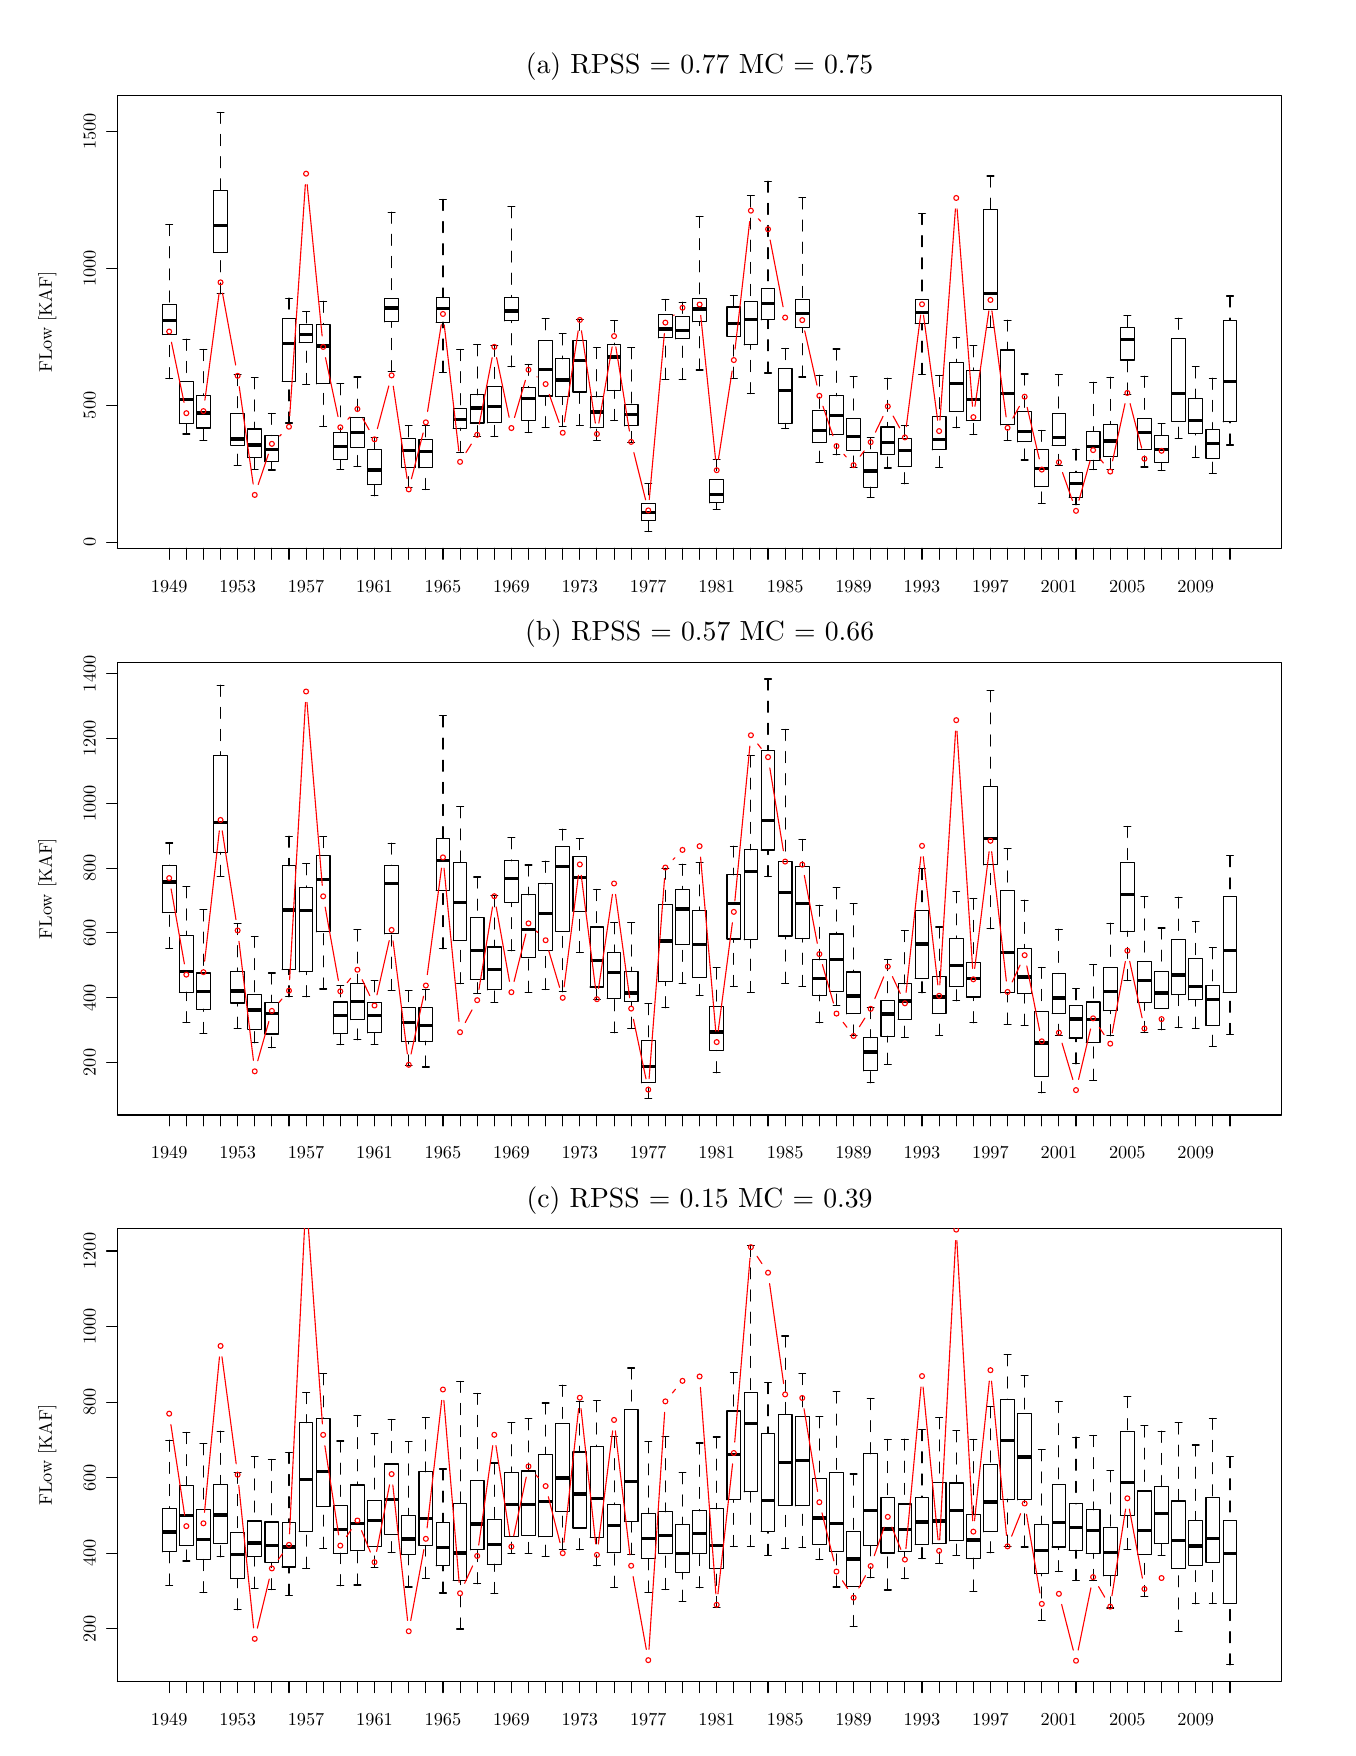
\begin{tikzpicture}[x=1pt,y=1pt]
\definecolor[named]{drawColor}{rgb}{0.00,0.00,0.00}
\definecolor[named]{fillColor}{rgb}{1.00,1.00,1.00}
\fill[color=fillColor,] (0,0) rectangle (469.75,614.29);
\begin{scope}
\path[clip] ( 32.47,426.16) rectangle (453.12,589.74);
\definecolor[named]{drawColor}{rgb}{0.00,0.00,0.00}

\draw[color=drawColor,line width= 1.2pt,line join=round,fill opacity=0.00,] ( 48.67,508.52) -- ( 53.62,508.52);

\draw[color=drawColor,dash pattern=on 4pt off 4pt ,line cap=round,line join=round,fill opacity=0.00,] ( 51.14,487.44) -- ( 51.14,503.37);

\draw[color=drawColor,dash pattern=on 4pt off 4pt ,line cap=round,line join=round,fill opacity=0.00,] ( 51.14,543.14) -- ( 51.14,514.16);

\draw[color=drawColor,line cap=round,line join=round,fill opacity=0.00,] ( 49.91,487.44) -- ( 52.38,487.44);

\draw[color=drawColor,line cap=round,line join=round,fill opacity=0.00,] ( 49.91,543.14) -- ( 52.38,543.14);

\draw[color=drawColor,line cap=round,line join=round,fill opacity=0.00,] ( 48.67,503.37) --
	( 53.62,503.37) --
	( 53.62,514.16) --
	( 48.67,514.16) --
	( 48.67,503.37);

\draw[color=drawColor,line width= 1.2pt,line join=round,fill opacity=0.00,] ( 54.85,479.86) -- ( 59.80,479.86);

\draw[color=drawColor,dash pattern=on 4pt off 4pt ,line cap=round,line join=round,fill opacity=0.00,] ( 57.33,467.45) -- ( 57.33,471.22);

\draw[color=drawColor,dash pattern=on 4pt off 4pt ,line cap=round,line join=round,fill opacity=0.00,] ( 57.33,501.69) -- ( 57.33,486.31);

\draw[color=drawColor,line cap=round,line join=round,fill opacity=0.00,] ( 56.09,467.45) -- ( 58.56,467.45);

\draw[color=drawColor,line cap=round,line join=round,fill opacity=0.00,] ( 56.09,501.69) -- ( 58.56,501.69);

\draw[color=drawColor,line cap=round,line join=round,fill opacity=0.00,] ( 54.85,471.22) --
	( 59.80,471.22) --
	( 59.80,486.31) --
	( 54.85,486.31) --
	( 54.85,471.22);

\draw[color=drawColor,line width= 1.2pt,line join=round,fill opacity=0.00,] ( 61.03,475.10) -- ( 65.98,475.10);

\draw[color=drawColor,dash pattern=on 4pt off 4pt ,line cap=round,line join=round,fill opacity=0.00,] ( 63.51,465.18) -- ( 63.51,469.61);

\draw[color=drawColor,dash pattern=on 4pt off 4pt ,line cap=round,line join=round,fill opacity=0.00,] ( 63.51,497.99) -- ( 63.51,481.31);

\draw[color=drawColor,line cap=round,line join=round,fill opacity=0.00,] ( 62.27,465.18) -- ( 64.74,465.18);

\draw[color=drawColor,line cap=round,line join=round,fill opacity=0.00,] ( 62.27,497.99) -- ( 64.74,497.99);

\draw[color=drawColor,line cap=round,line join=round,fill opacity=0.00,] ( 61.03,469.61) --
	( 65.98,469.61) --
	( 65.98,481.31) --
	( 61.03,481.31) --
	( 61.03,469.61);

\draw[color=drawColor,line width= 1.2pt,line join=round,fill opacity=0.00,] ( 67.22,542.86) -- ( 72.16,542.86);

\draw[color=drawColor,dash pattern=on 4pt off 4pt ,line cap=round,line join=round,fill opacity=0.00,] ( 69.69,518.07) -- ( 69.69,533.05);

\draw[color=drawColor,dash pattern=on 4pt off 4pt ,line cap=round,line join=round,fill opacity=0.00,] ( 69.69,583.68) -- ( 69.69,555.37);

\draw[color=drawColor,line cap=round,line join=round,fill opacity=0.00,] ( 68.45,518.07) -- ( 70.93,518.07);

\draw[color=drawColor,line cap=round,line join=round,fill opacity=0.00,] ( 68.45,583.68) -- ( 70.93,583.68);

\draw[color=drawColor,line cap=round,line join=round,fill opacity=0.00,] ( 67.22,533.05) --
	( 72.16,533.05) --
	( 72.16,555.37) --
	( 67.22,555.37) --
	( 67.22,533.05);

\draw[color=drawColor,line width= 1.2pt,line join=round,fill opacity=0.00,] ( 73.40,465.68) -- ( 78.35,465.68);

\draw[color=drawColor,dash pattern=on 4pt off 4pt ,line cap=round,line join=round,fill opacity=0.00,] ( 75.87,456.18) -- ( 75.87,463.45);

\draw[color=drawColor,dash pattern=on 4pt off 4pt ,line cap=round,line join=round,fill opacity=0.00,] ( 75.87,488.96) -- ( 75.87,474.75);

\draw[color=drawColor,line cap=round,line join=round,fill opacity=0.00,] ( 74.64,456.18) -- ( 77.11,456.18);

\draw[color=drawColor,line cap=round,line join=round,fill opacity=0.00,] ( 74.64,488.96) -- ( 77.11,488.96);

\draw[color=drawColor,line cap=round,line join=round,fill opacity=0.00,] ( 73.40,463.45) --
	( 78.35,463.45) --
	( 78.35,474.75) --
	( 73.40,474.75) --
	( 73.40,463.45);

\draw[color=drawColor,line width= 1.2pt,line join=round,fill opacity=0.00,] ( 79.58,463.47) -- ( 84.53,463.47);

\draw[color=drawColor,dash pattern=on 4pt off 4pt ,line cap=round,line join=round,fill opacity=0.00,] ( 82.05,454.74) -- ( 82.05,458.95);

\draw[color=drawColor,dash pattern=on 4pt off 4pt ,line cap=round,line join=round,fill opacity=0.00,] ( 82.05,487.75) -- ( 82.05,469.27);

\draw[color=drawColor,line cap=round,line join=round,fill opacity=0.00,] ( 80.82,454.74) -- ( 83.29,454.74);

\draw[color=drawColor,line cap=round,line join=round,fill opacity=0.00,] ( 80.82,487.75) -- ( 83.29,487.75);

\draw[color=drawColor,line cap=round,line join=round,fill opacity=0.00,] ( 79.58,458.95) --
	( 84.53,458.95) --
	( 84.53,469.27) --
	( 79.58,469.27) --
	( 79.58,458.95);

\draw[color=drawColor,line width= 1.2pt,line join=round,fill opacity=0.00,] ( 85.76,461.82) -- ( 90.71,461.82);

\draw[color=drawColor,dash pattern=on 4pt off 4pt ,line cap=round,line join=round,fill opacity=0.00,] ( 88.24,454.44) -- ( 88.24,457.41);

\draw[color=drawColor,dash pattern=on 4pt off 4pt ,line cap=round,line join=round,fill opacity=0.00,] ( 88.24,474.93) -- ( 88.24,466.91);

\draw[color=drawColor,line cap=round,line join=round,fill opacity=0.00,] ( 87.00,454.44) -- ( 89.47,454.44);

\draw[color=drawColor,line cap=round,line join=round,fill opacity=0.00,] ( 87.00,474.93) -- ( 89.47,474.93);

\draw[color=drawColor,line cap=round,line join=round,fill opacity=0.00,] ( 85.76,457.41) --
	( 90.71,457.41) --
	( 90.71,466.91) --
	( 85.76,466.91) --
	( 85.76,457.41);

\draw[color=drawColor,line width= 1.2pt,line join=round,fill opacity=0.00,] ( 91.95,500.12) -- ( 96.89,500.12);

\draw[color=drawColor,dash pattern=on 4pt off 4pt ,line cap=round,line join=round,fill opacity=0.00,] ( 94.42,471.42) -- ( 94.42,486.57);

\draw[color=drawColor,dash pattern=on 4pt off 4pt ,line cap=round,line join=round,fill opacity=0.00,] ( 94.42,516.58) -- ( 94.42,509.19);

\draw[color=drawColor,line cap=round,line join=round,fill opacity=0.00,] ( 93.18,471.42) -- ( 95.66,471.42);

\draw[color=drawColor,line cap=round,line join=round,fill opacity=0.00,] ( 93.18,516.58) -- ( 95.66,516.58);

\draw[color=drawColor,line cap=round,line join=round,fill opacity=0.00,] ( 91.95,486.57) --
	( 96.89,486.57) --
	( 96.89,509.19) --
	( 91.95,509.19) --
	( 91.95,486.57);

\draw[color=drawColor,line width= 1.2pt,line join=round,fill opacity=0.00,] ( 98.13,503.35) -- (103.08,503.35);

\draw[color=drawColor,dash pattern=on 4pt off 4pt ,line cap=round,line join=round,fill opacity=0.00,] (100.60,485.38) -- (100.60,500.53);

\draw[color=drawColor,dash pattern=on 4pt off 4pt ,line cap=round,line join=round,fill opacity=0.00,] (100.60,511.58) -- (100.60,506.99);

\draw[color=drawColor,line cap=round,line join=round,fill opacity=0.00,] ( 99.37,485.38) -- (101.84,485.38);

\draw[color=drawColor,line cap=round,line join=round,fill opacity=0.00,] ( 99.37,511.58) -- (101.84,511.58);

\draw[color=drawColor,line cap=round,line join=round,fill opacity=0.00,] ( 98.13,500.53) --
	(103.08,500.53) --
	(103.08,506.99) --
	( 98.13,506.99) --
	( 98.13,500.53);

\draw[color=drawColor,line width= 1.2pt,line join=round,fill opacity=0.00,] (104.31,499.20) -- (109.26,499.20);

\draw[color=drawColor,dash pattern=on 4pt off 4pt ,line cap=round,line join=round,fill opacity=0.00,] (106.78,470.13) -- (106.78,485.57);

\draw[color=drawColor,dash pattern=on 4pt off 4pt ,line cap=round,line join=round,fill opacity=0.00,] (106.78,515.41) -- (106.78,507.08);

\draw[color=drawColor,line cap=round,line join=round,fill opacity=0.00,] (105.55,470.13) -- (108.02,470.13);

\draw[color=drawColor,line cap=round,line join=round,fill opacity=0.00,] (105.55,515.41) -- (108.02,515.41);

\draw[color=drawColor,line cap=round,line join=round,fill opacity=0.00,] (104.31,485.57) --
	(109.26,485.57) --
	(109.26,507.08) --
	(104.31,507.08) --
	(104.31,485.57);

\draw[color=drawColor,line width= 1.2pt,line join=round,fill opacity=0.00,] (110.49,462.83) -- (115.44,462.83);

\draw[color=drawColor,dash pattern=on 4pt off 4pt ,line cap=round,line join=round,fill opacity=0.00,] (112.97,454.65) -- (112.97,458.19);

\draw[color=drawColor,dash pattern=on 4pt off 4pt ,line cap=round,line join=round,fill opacity=0.00,] (112.97,485.63) -- (112.97,467.99);

\draw[color=drawColor,line cap=round,line join=round,fill opacity=0.00,] (111.73,454.65) -- (114.20,454.65);

\draw[color=drawColor,line cap=round,line join=round,fill opacity=0.00,] (111.73,485.63) -- (114.20,485.63);

\draw[color=drawColor,line cap=round,line join=round,fill opacity=0.00,] (110.49,458.19) --
	(115.44,458.19) --
	(115.44,467.99) --
	(110.49,467.99) --
	(110.49,458.19);

\draw[color=drawColor,line width= 1.2pt,line join=round,fill opacity=0.00,] (116.68,468.05) -- (121.62,468.05);

\draw[color=drawColor,dash pattern=on 4pt off 4pt ,line cap=round,line join=round,fill opacity=0.00,] (119.15,455.68) -- (119.15,462.63);

\draw[color=drawColor,dash pattern=on 4pt off 4pt ,line cap=round,line join=round,fill opacity=0.00,] (119.15,488.04) -- (119.15,473.54);

\draw[color=drawColor,line cap=round,line join=round,fill opacity=0.00,] (117.91,455.68) -- (120.39,455.68);

\draw[color=drawColor,line cap=round,line join=round,fill opacity=0.00,] (117.91,488.04) -- (120.39,488.04);

\draw[color=drawColor,line cap=round,line join=round,fill opacity=0.00,] (116.68,462.63) --
	(121.62,462.63) --
	(121.62,473.54) --
	(116.68,473.54) --
	(116.68,462.63);

\draw[color=drawColor,line width= 1.2pt,line join=round,fill opacity=0.00,] (122.86,454.42) -- (127.80,454.42);

\draw[color=drawColor,dash pattern=on 4pt off 4pt ,line cap=round,line join=round,fill opacity=0.00,] (125.33,445.08) -- (125.33,449.20);

\draw[color=drawColor,dash pattern=on 4pt off 4pt ,line cap=round,line join=round,fill opacity=0.00,] (125.33,466.07) -- (125.33,462.01);

\draw[color=drawColor,line cap=round,line join=round,fill opacity=0.00,] (124.10,445.08) -- (126.57,445.08);

\draw[color=drawColor,line cap=round,line join=round,fill opacity=0.00,] (124.10,466.07) -- (126.57,466.07);

\draw[color=drawColor,line cap=round,line join=round,fill opacity=0.00,] (122.86,449.20) --
	(127.80,449.20) --
	(127.80,462.01) --
	(122.86,462.01) --
	(122.86,449.20);

\draw[color=drawColor,line width= 1.2pt,line join=round,fill opacity=0.00,] (129.04,513.03) -- (133.99,513.03);

\draw[color=drawColor,dash pattern=on 4pt off 4pt ,line cap=round,line join=round,fill opacity=0.00,] (131.51,489.99) -- (131.51,507.99);

\draw[color=drawColor,dash pattern=on 4pt off 4pt ,line cap=round,line join=round,fill opacity=0.00,] (131.51,547.62) -- (131.51,516.30);

\draw[color=drawColor,line cap=round,line join=round,fill opacity=0.00,] (130.28,489.99) -- (132.75,489.99);

\draw[color=drawColor,line cap=round,line join=round,fill opacity=0.00,] (130.28,547.62) -- (132.75,547.62);

\draw[color=drawColor,line cap=round,line join=round,fill opacity=0.00,] (129.04,507.99) --
	(133.99,507.99) --
	(133.99,516.30) --
	(129.04,516.30) --
	(129.04,507.99);

\draw[color=drawColor,line width= 1.2pt,line join=round,fill opacity=0.00,] (135.22,461.38) -- (140.17,461.38);

\draw[color=drawColor,dash pattern=on 4pt off 4pt ,line cap=round,line join=round,fill opacity=0.00,] (137.70,448.07) -- (137.70,455.40);

\draw[color=drawColor,dash pattern=on 4pt off 4pt ,line cap=round,line join=round,fill opacity=0.00,] (137.70,470.47) -- (137.70,465.70);

\draw[color=drawColor,line cap=round,line join=round,fill opacity=0.00,] (136.46,448.07) -- (138.93,448.07);

\draw[color=drawColor,line cap=round,line join=round,fill opacity=0.00,] (136.46,470.47) -- (138.93,470.47);

\draw[color=drawColor,line cap=round,line join=round,fill opacity=0.00,] (135.22,455.40) --
	(140.17,455.40) --
	(140.17,465.70) --
	(135.22,465.70) --
	(135.22,455.40);

\draw[color=drawColor,line width= 1.2pt,line join=round,fill opacity=0.00,] (141.41,461.22) -- (146.35,461.22);

\draw[color=drawColor,dash pattern=on 4pt off 4pt ,line cap=round,line join=round,fill opacity=0.00,] (143.88,447.37) -- (143.88,455.23);

\draw[color=drawColor,dash pattern=on 4pt off 4pt ,line cap=round,line join=round,fill opacity=0.00,] (143.88,470.42) -- (143.88,465.51);

\draw[color=drawColor,line cap=round,line join=round,fill opacity=0.00,] (142.64,447.37) -- (145.12,447.37);

\draw[color=drawColor,line cap=round,line join=round,fill opacity=0.00,] (142.64,470.42) -- (145.12,470.42);

\draw[color=drawColor,line cap=round,line join=round,fill opacity=0.00,] (141.41,455.23) --
	(146.35,455.23) --
	(146.35,465.51) --
	(141.41,465.51) --
	(141.41,455.23);

\draw[color=drawColor,line width= 1.2pt,line join=round,fill opacity=0.00,] (147.59,512.90) -- (152.53,512.90);

\draw[color=drawColor,dash pattern=on 4pt off 4pt ,line cap=round,line join=round,fill opacity=0.00,] (150.06,489.81) -- (150.06,507.89);

\draw[color=drawColor,dash pattern=on 4pt off 4pt ,line cap=round,line join=round,fill opacity=0.00,] (150.06,552.23) -- (150.06,516.73);

\draw[color=drawColor,line cap=round,line join=round,fill opacity=0.00,] (148.82,489.81) -- (151.30,489.81);

\draw[color=drawColor,line cap=round,line join=round,fill opacity=0.00,] (148.82,552.23) -- (151.30,552.23);

\draw[color=drawColor,line cap=round,line join=round,fill opacity=0.00,] (147.59,507.89) --
	(152.53,507.89) --
	(152.53,516.73) --
	(147.59,516.73) --
	(147.59,507.89);

\draw[color=drawColor,line width= 1.2pt,line join=round,fill opacity=0.00,] (153.77,472.75) -- (158.72,472.75);

\draw[color=drawColor,dash pattern=on 4pt off 4pt ,line cap=round,line join=round,fill opacity=0.00,] (156.24,460.77) -- (156.24,469.55);

\draw[color=drawColor,dash pattern=on 4pt off 4pt ,line cap=round,line join=round,fill opacity=0.00,] (156.24,498.00) -- (156.24,476.73);

\draw[color=drawColor,line cap=round,line join=round,fill opacity=0.00,] (155.01,460.77) -- (157.48,460.77);

\draw[color=drawColor,line cap=round,line join=round,fill opacity=0.00,] (155.01,498.00) -- (157.48,498.00);

\draw[color=drawColor,line cap=round,line join=round,fill opacity=0.00,] (153.77,469.55) --
	(158.72,469.55) --
	(158.72,476.73) --
	(153.77,476.73) --
	(153.77,469.55);

\draw[color=drawColor,line width= 1.2pt,line join=round,fill opacity=0.00,] (159.95,476.86) -- (164.90,476.86);

\draw[color=drawColor,dash pattern=on 4pt off 4pt ,line cap=round,line join=round,fill opacity=0.00,] (162.43,466.46) -- (162.43,471.44);

\draw[color=drawColor,dash pattern=on 4pt off 4pt ,line cap=round,line join=round,fill opacity=0.00,] (162.43,499.67) -- (162.43,481.58);

\draw[color=drawColor,line cap=round,line join=round,fill opacity=0.00,] (161.19,466.46) -- (163.66,466.46);

\draw[color=drawColor,line cap=round,line join=round,fill opacity=0.00,] (161.19,499.67) -- (163.66,499.67);

\draw[color=drawColor,line cap=round,line join=round,fill opacity=0.00,] (159.95,471.44) --
	(164.90,471.44) --
	(164.90,481.58) --
	(159.95,481.58) --
	(159.95,471.44);

\draw[color=drawColor,line width= 1.2pt,line join=round,fill opacity=0.00,] (166.14,477.29) -- (171.08,477.29);

\draw[color=drawColor,dash pattern=on 4pt off 4pt ,line cap=round,line join=round,fill opacity=0.00,] (168.61,466.57) -- (168.61,471.51);

\draw[color=drawColor,dash pattern=on 4pt off 4pt ,line cap=round,line join=round,fill opacity=0.00,] (168.61,499.52) -- (168.61,484.54);

\draw[color=drawColor,line cap=round,line join=round,fill opacity=0.00,] (167.37,466.57) -- (169.85,466.57);

\draw[color=drawColor,line cap=round,line join=round,fill opacity=0.00,] (167.37,499.52) -- (169.85,499.52);

\draw[color=drawColor,line cap=round,line join=round,fill opacity=0.00,] (166.14,471.51) --
	(171.08,471.51) --
	(171.08,484.54) --
	(166.14,484.54) --
	(166.14,471.51);

\draw[color=drawColor,line width= 1.2pt,line join=round,fill opacity=0.00,] (172.32,511.96) -- (177.26,511.96);

\draw[color=drawColor,dash pattern=on 4pt off 4pt ,line cap=round,line join=round,fill opacity=0.00,] (174.79,491.69) -- (174.79,508.34);

\draw[color=drawColor,dash pattern=on 4pt off 4pt ,line cap=round,line join=round,fill opacity=0.00,] (174.79,549.55) -- (174.79,516.91);

\draw[color=drawColor,line cap=round,line join=round,fill opacity=0.00,] (173.55,491.69) -- (176.03,491.69);

\draw[color=drawColor,line cap=round,line join=round,fill opacity=0.00,] (173.55,549.55) -- (176.03,549.55);

\draw[color=drawColor,line cap=round,line join=round,fill opacity=0.00,] (172.32,508.34) --
	(177.26,508.34) --
	(177.26,516.91) --
	(172.32,516.91) --
	(172.32,508.34);

\draw[color=drawColor,line width= 1.2pt,line join=round,fill opacity=0.00,] (178.50,480.18) -- (183.45,480.18);

\draw[color=drawColor,dash pattern=on 4pt off 4pt ,line cap=round,line join=round,fill opacity=0.00,] (180.97,467.98) -- (180.97,472.38);

\draw[color=drawColor,dash pattern=on 4pt off 4pt ,line cap=round,line join=round,fill opacity=0.00,] (180.97,492.62) -- (180.97,484.22);

\draw[color=drawColor,line cap=round,line join=round,fill opacity=0.00,] (179.74,467.98) -- (182.21,467.98);

\draw[color=drawColor,line cap=round,line join=round,fill opacity=0.00,] (179.74,492.62) -- (182.21,492.62);

\draw[color=drawColor,line cap=round,line join=round,fill opacity=0.00,] (178.50,472.38) --
	(183.45,472.38) --
	(183.45,484.22) --
	(178.50,484.22) --
	(178.50,472.38);

\draw[color=drawColor,line width= 1.2pt,line join=round,fill opacity=0.00,] (184.68,490.85) -- (189.63,490.85);

\draw[color=drawColor,dash pattern=on 4pt off 4pt ,line cap=round,line join=round,fill opacity=0.00,] (187.16,469.77) -- (187.16,481.18);

\draw[color=drawColor,dash pattern=on 4pt off 4pt ,line cap=round,line join=round,fill opacity=0.00,] (187.16,509.07) -- (187.16,501.10);

\draw[color=drawColor,line cap=round,line join=round,fill opacity=0.00,] (185.92,469.77) -- (188.39,469.77);

\draw[color=drawColor,line cap=round,line join=round,fill opacity=0.00,] (185.92,509.07) -- (188.39,509.07);

\draw[color=drawColor,line cap=round,line join=round,fill opacity=0.00,] (184.68,481.18) --
	(189.63,481.18) --
	(189.63,501.10) --
	(184.68,501.10) --
	(184.68,481.18);

\draw[color=drawColor,line width= 1.2pt,line join=round,fill opacity=0.00,] (190.87,486.93) -- (195.81,486.93);

\draw[color=drawColor,dash pattern=on 4pt off 4pt ,line cap=round,line join=round,fill opacity=0.00,] (193.34,470.11) -- (193.34,480.95);

\draw[color=drawColor,dash pattern=on 4pt off 4pt ,line cap=round,line join=round,fill opacity=0.00,] (193.34,503.63) -- (193.34,494.62);

\draw[color=drawColor,line cap=round,line join=round,fill opacity=0.00,] (192.10,470.11) -- (194.57,470.11);

\draw[color=drawColor,line cap=round,line join=round,fill opacity=0.00,] (192.10,503.63) -- (194.57,503.63);

\draw[color=drawColor,line cap=round,line join=round,fill opacity=0.00,] (190.87,480.95) --
	(195.81,480.95) --
	(195.81,494.62) --
	(190.87,494.62) --
	(190.87,480.95);

\draw[color=drawColor,line width= 1.2pt,line join=round,fill opacity=0.00,] (197.05,493.96) -- (201.99,493.96);

\draw[color=drawColor,dash pattern=on 4pt off 4pt ,line cap=round,line join=round,fill opacity=0.00,] (199.52,470.50) -- (199.52,482.64);

\draw[color=drawColor,dash pattern=on 4pt off 4pt ,line cap=round,line join=round,fill opacity=0.00,] (199.52,508.90) -- (199.52,501.28);

\draw[color=drawColor,line cap=round,line join=round,fill opacity=0.00,] (198.28,470.50) -- (200.76,470.50);

\draw[color=drawColor,line cap=round,line join=round,fill opacity=0.00,] (198.28,508.90) -- (200.76,508.90);

\draw[color=drawColor,line cap=round,line join=round,fill opacity=0.00,] (197.05,482.64) --
	(201.99,482.64) --
	(201.99,501.28) --
	(197.05,501.28) --
	(197.05,482.64);

\draw[color=drawColor,line width= 1.2pt,line join=round,fill opacity=0.00,] (203.23,475.45) -- (208.18,475.45);

\draw[color=drawColor,dash pattern=on 4pt off 4pt ,line cap=round,line join=round,fill opacity=0.00,] (205.70,465.17) -- (205.70,469.72);

\draw[color=drawColor,dash pattern=on 4pt off 4pt ,line cap=round,line join=round,fill opacity=0.00,] (205.70,498.67) -- (205.70,480.89);

\draw[color=drawColor,line cap=round,line join=round,fill opacity=0.00,] (204.47,465.17) -- (206.94,465.17);

\draw[color=drawColor,line cap=round,line join=round,fill opacity=0.00,] (204.47,498.67) -- (206.94,498.67);

\draw[color=drawColor,line cap=round,line join=round,fill opacity=0.00,] (203.23,469.72) --
	(208.18,469.72) --
	(208.18,480.89) --
	(203.23,480.89) --
	(203.23,469.72);

\draw[color=drawColor,line width= 1.2pt,line join=round,fill opacity=0.00,] (209.41,495.29) -- (214.36,495.29);

\draw[color=drawColor,dash pattern=on 4pt off 4pt ,line cap=round,line join=round,fill opacity=0.00,] (211.89,472.35) -- (211.89,483.16);

\draw[color=drawColor,dash pattern=on 4pt off 4pt ,line cap=round,line join=round,fill opacity=0.00,] (211.89,508.32) -- (211.89,499.70);

\draw[color=drawColor,line cap=round,line join=round,fill opacity=0.00,] (210.65,472.35) -- (213.12,472.35);

\draw[color=drawColor,line cap=round,line join=round,fill opacity=0.00,] (210.65,508.32) -- (213.12,508.32);

\draw[color=drawColor,line cap=round,line join=round,fill opacity=0.00,] (209.41,483.16) --
	(214.36,483.16) --
	(214.36,499.70) --
	(209.41,499.70) --
	(209.41,483.16);

\draw[color=drawColor,line width= 1.2pt,line join=round,fill opacity=0.00,] (215.59,474.55) -- (220.54,474.55);

\draw[color=drawColor,dash pattern=on 4pt off 4pt ,line cap=round,line join=round,fill opacity=0.00,] (218.07,464.38) -- (218.07,470.39);

\draw[color=drawColor,dash pattern=on 4pt off 4pt ,line cap=round,line join=round,fill opacity=0.00,] (218.07,498.60) -- (218.07,478.15);

\draw[color=drawColor,line cap=round,line join=round,fill opacity=0.00,] (216.83,464.38) -- (219.30,464.38);

\draw[color=drawColor,line cap=round,line join=round,fill opacity=0.00,] (216.83,498.60) -- (219.30,498.60);

\draw[color=drawColor,line cap=round,line join=round,fill opacity=0.00,] (215.59,470.39) --
	(220.54,470.39) --
	(220.54,478.15) --
	(215.59,478.15) --
	(215.59,470.39);

\draw[color=drawColor,line width= 1.2pt,line join=round,fill opacity=0.00,] (221.78,439.20) -- (226.72,439.20);

\draw[color=drawColor,dash pattern=on 4pt off 4pt ,line cap=round,line join=round,fill opacity=0.00,] (224.25,432.22) -- (224.25,436.14);

\draw[color=drawColor,dash pattern=on 4pt off 4pt ,line cap=round,line join=round,fill opacity=0.00,] (224.25,449.48) -- (224.25,442.41);

\draw[color=drawColor,line cap=round,line join=round,fill opacity=0.00,] (223.01,432.22) -- (225.49,432.22);

\draw[color=drawColor,line cap=round,line join=round,fill opacity=0.00,] (223.01,449.48) -- (225.49,449.48);

\draw[color=drawColor,line cap=round,line join=round,fill opacity=0.00,] (221.78,436.14) --
	(226.72,436.14) --
	(226.72,442.41) --
	(221.78,442.41) --
	(221.78,436.14);

\draw[color=drawColor,line width= 1.2pt,line join=round,fill opacity=0.00,] (227.96,505.39) -- (232.91,505.39);

\draw[color=drawColor,dash pattern=on 4pt off 4pt ,line cap=round,line join=round,fill opacity=0.00,] (230.43,487.24) -- (230.43,502.23);

\draw[color=drawColor,dash pattern=on 4pt off 4pt ,line cap=round,line join=round,fill opacity=0.00,] (230.43,516.06) -- (230.43,510.72);

\draw[color=drawColor,line cap=round,line join=round,fill opacity=0.00,] (229.20,487.24) -- (231.67,487.24);

\draw[color=drawColor,line cap=round,line join=round,fill opacity=0.00,] (229.20,516.06) -- (231.67,516.06);

\draw[color=drawColor,line cap=round,line join=round,fill opacity=0.00,] (227.96,502.23) --
	(232.91,502.23) --
	(232.91,510.72) --
	(227.96,510.72) --
	(227.96,502.23);

\draw[color=drawColor,line width= 1.2pt,line join=round,fill opacity=0.00,] (234.14,504.74) -- (239.09,504.74);

\draw[color=drawColor,dash pattern=on 4pt off 4pt ,line cap=round,line join=round,fill opacity=0.00,] (236.62,487.16) -- (236.62,501.81);

\draw[color=drawColor,dash pattern=on 4pt off 4pt ,line cap=round,line join=round,fill opacity=0.00,] (236.62,515.06) -- (236.62,509.84);

\draw[color=drawColor,line cap=round,line join=round,fill opacity=0.00,] (235.38,487.16) -- (237.85,487.16);

\draw[color=drawColor,line cap=round,line join=round,fill opacity=0.00,] (235.38,515.06) -- (237.85,515.06);

\draw[color=drawColor,line cap=round,line join=round,fill opacity=0.00,] (234.14,501.81) --
	(239.09,501.81) --
	(239.09,509.84) --
	(234.14,509.84) --
	(234.14,501.81);

\draw[color=drawColor,line width= 1.2pt,line join=round,fill opacity=0.00,] (240.32,512.67) -- (245.27,512.67);

\draw[color=drawColor,dash pattern=on 4pt off 4pt ,line cap=round,line join=round,fill opacity=0.00,] (242.80,490.60) -- (242.80,508.03);

\draw[color=drawColor,dash pattern=on 4pt off 4pt ,line cap=round,line join=round,fill opacity=0.00,] (242.80,546.07) -- (242.80,516.54);

\draw[color=drawColor,line cap=round,line join=round,fill opacity=0.00,] (241.56,490.60) -- (244.03,490.60);

\draw[color=drawColor,line cap=round,line join=round,fill opacity=0.00,] (241.56,546.07) -- (244.03,546.07);

\draw[color=drawColor,line cap=round,line join=round,fill opacity=0.00,] (240.32,508.03) --
	(245.27,508.03) --
	(245.27,516.54) --
	(240.32,516.54) --
	(240.32,508.03);

\draw[color=drawColor,line width= 1.2pt,line join=round,fill opacity=0.00,] (246.51,445.54) -- (251.45,445.54);

\draw[color=drawColor,dash pattern=on 4pt off 4pt ,line cap=round,line join=round,fill opacity=0.00,] (248.98,440.32) -- (248.98,442.61);

\draw[color=drawColor,dash pattern=on 4pt off 4pt ,line cap=round,line join=round,fill opacity=0.00,] (248.98,458.22) -- (248.98,451.01);

\draw[color=drawColor,line cap=round,line join=round,fill opacity=0.00,] (247.74,440.32) -- (250.22,440.32);

\draw[color=drawColor,line cap=round,line join=round,fill opacity=0.00,] (247.74,458.22) -- (250.22,458.22);

\draw[color=drawColor,line cap=round,line join=round,fill opacity=0.00,] (246.51,442.61) --
	(251.45,442.61) --
	(251.45,451.01) --
	(246.51,451.01) --
	(246.51,442.61);

\draw[color=drawColor,line width= 1.2pt,line join=round,fill opacity=0.00,] (252.69,507.32) -- (257.64,507.32);

\draw[color=drawColor,dash pattern=on 4pt off 4pt ,line cap=round,line join=round,fill opacity=0.00,] (255.16,487.61) -- (255.16,502.82);

\draw[color=drawColor,dash pattern=on 4pt off 4pt ,line cap=round,line join=round,fill opacity=0.00,] (255.16,517.56) -- (255.16,513.33);

\draw[color=drawColor,line cap=round,line join=round,fill opacity=0.00,] (253.93,487.61) -- (256.40,487.61);

\draw[color=drawColor,line cap=round,line join=round,fill opacity=0.00,] (253.93,517.56) -- (256.40,517.56);

\draw[color=drawColor,line cap=round,line join=round,fill opacity=0.00,] (252.69,502.82) --
	(257.64,502.82) --
	(257.64,513.33) --
	(252.69,513.33) --
	(252.69,502.82);

\draw[color=drawColor,line width= 1.2pt,line join=round,fill opacity=0.00,] (258.87,508.76) -- (263.82,508.76);

\draw[color=drawColor,dash pattern=on 4pt off 4pt ,line cap=round,line join=round,fill opacity=0.00,] (261.34,482.02) -- (261.34,499.65);

\draw[color=drawColor,dash pattern=on 4pt off 4pt ,line cap=round,line join=round,fill opacity=0.00,] (261.34,553.48) -- (261.34,515.37);

\draw[color=drawColor,line cap=round,line join=round,fill opacity=0.00,] (260.11,482.02) -- (262.58,482.02);

\draw[color=drawColor,line cap=round,line join=round,fill opacity=0.00,] (260.11,553.48) -- (262.58,553.48);

\draw[color=drawColor,line cap=round,line join=round,fill opacity=0.00,] (258.87,499.65) --
	(263.82,499.65) --
	(263.82,515.37) --
	(258.87,515.37) --
	(258.87,499.65);

\draw[color=drawColor,line width= 1.2pt,line join=round,fill opacity=0.00,] (265.05,514.59) -- (270.00,514.59);

\draw[color=drawColor,dash pattern=on 4pt off 4pt ,line cap=round,line join=round,fill opacity=0.00,] (267.53,489.51) -- (267.53,508.73);

\draw[color=drawColor,dash pattern=on 4pt off 4pt ,line cap=round,line join=round,fill opacity=0.00,] (267.53,558.80) -- (267.53,519.94);

\draw[color=drawColor,line cap=round,line join=round,fill opacity=0.00,] (266.29,489.51) -- (268.76,489.51);

\draw[color=drawColor,line cap=round,line join=round,fill opacity=0.00,] (266.29,558.80) -- (268.76,558.80);

\draw[color=drawColor,line cap=round,line join=round,fill opacity=0.00,] (265.05,508.73) --
	(270.00,508.73) --
	(270.00,519.94) --
	(265.05,519.94) --
	(265.05,508.73);

\draw[color=drawColor,line width= 1.2pt,line join=round,fill opacity=0.00,] (271.24,483.12) -- (276.18,483.12);

\draw[color=drawColor,dash pattern=on 4pt off 4pt ,line cap=round,line join=round,fill opacity=0.00,] (273.71,469.44) -- (273.71,471.27);

\draw[color=drawColor,dash pattern=on 4pt off 4pt ,line cap=round,line join=round,fill opacity=0.00,] (273.71,498.36) -- (273.71,491.16);

\draw[color=drawColor,line cap=round,line join=round,fill opacity=0.00,] (272.47,469.44) -- (274.95,469.44);

\draw[color=drawColor,line cap=round,line join=round,fill opacity=0.00,] (272.47,498.36) -- (274.95,498.36);

\draw[color=drawColor,line cap=round,line join=round,fill opacity=0.00,] (271.24,471.27) --
	(276.18,471.27) --
	(276.18,491.16) --
	(271.24,491.16) --
	(271.24,471.27);

\draw[color=drawColor,line width= 1.2pt,line join=round,fill opacity=0.00,] (277.42,510.98) -- (282.36,510.98);

\draw[color=drawColor,dash pattern=on 4pt off 4pt ,line cap=round,line join=round,fill opacity=0.00,] (279.89,488.07) -- (279.89,505.91);

\draw[color=drawColor,dash pattern=on 4pt off 4pt ,line cap=round,line join=round,fill opacity=0.00,] (279.89,552.77) -- (279.89,516.04);

\draw[color=drawColor,line cap=round,line join=round,fill opacity=0.00,] (278.66,488.07) -- (281.13,488.07);

\draw[color=drawColor,line cap=round,line join=round,fill opacity=0.00,] (278.66,552.77) -- (281.13,552.77);

\draw[color=drawColor,line cap=round,line join=round,fill opacity=0.00,] (277.42,505.91) --
	(282.36,505.91) --
	(282.36,516.04) --
	(277.42,516.04) --
	(277.42,505.91);

\draw[color=drawColor,line width= 1.2pt,line join=round,fill opacity=0.00,] (283.60,468.71) -- (288.55,468.71);

\draw[color=drawColor,dash pattern=on 4pt off 4pt ,line cap=round,line join=round,fill opacity=0.00,] (286.07,457.28) -- (286.07,464.32);

\draw[color=drawColor,dash pattern=on 4pt off 4pt ,line cap=round,line join=round,fill opacity=0.00,] (286.07,488.74) -- (286.07,475.79);

\draw[color=drawColor,line cap=round,line join=round,fill opacity=0.00,] (284.84,457.28) -- (287.31,457.28);

\draw[color=drawColor,line cap=round,line join=round,fill opacity=0.00,] (284.84,488.74) -- (287.31,488.74);

\draw[color=drawColor,line cap=round,line join=round,fill opacity=0.00,] (283.60,464.32) --
	(288.55,464.32) --
	(288.55,475.79) --
	(283.60,475.79) --
	(283.60,464.32);

\draw[color=drawColor,line width= 1.2pt,line join=round,fill opacity=0.00,] (289.78,474.11) -- (294.73,474.11);

\draw[color=drawColor,dash pattern=on 4pt off 4pt ,line cap=round,line join=round,fill opacity=0.00,] (292.26,459.89) -- (292.26,467.14);

\draw[color=drawColor,dash pattern=on 4pt off 4pt ,line cap=round,line join=round,fill opacity=0.00,] (292.26,498.16) -- (292.26,481.26);

\draw[color=drawColor,line cap=round,line join=round,fill opacity=0.00,] (291.02,459.89) -- (293.49,459.89);

\draw[color=drawColor,line cap=round,line join=round,fill opacity=0.00,] (291.02,498.16) -- (293.49,498.16);

\draw[color=drawColor,line cap=round,line join=round,fill opacity=0.00,] (289.78,467.14) --
	(294.73,467.14) --
	(294.73,481.26) --
	(289.78,481.26) --
	(289.78,467.14);

\draw[color=drawColor,line width= 1.2pt,line join=round,fill opacity=0.00,] (295.97,466.55) -- (300.91,466.55);

\draw[color=drawColor,dash pattern=on 4pt off 4pt ,line cap=round,line join=round,fill opacity=0.00,] (298.44,455.50) -- (298.44,461.64);

\draw[color=drawColor,dash pattern=on 4pt off 4pt ,line cap=round,line join=round,fill opacity=0.00,] (298.44,488.13) -- (298.44,473.16);

\draw[color=drawColor,line cap=round,line join=round,fill opacity=0.00,] (297.20,455.50) -- (299.68,455.50);

\draw[color=drawColor,line cap=round,line join=round,fill opacity=0.00,] (297.20,488.13) -- (299.68,488.13);

\draw[color=drawColor,line cap=round,line join=round,fill opacity=0.00,] (295.97,461.64) --
	(300.91,461.64) --
	(300.91,473.16) --
	(295.97,473.16) --
	(295.97,461.64);

\draw[color=drawColor,line width= 1.2pt,line join=round,fill opacity=0.00,] (302.15,454.04) -- (307.09,454.04);

\draw[color=drawColor,dash pattern=on 4pt off 4pt ,line cap=round,line join=round,fill opacity=0.00,] (304.62,444.49) -- (304.62,448.27);

\draw[color=drawColor,dash pattern=on 4pt off 4pt ,line cap=round,line join=round,fill opacity=0.00,] (304.62,466.09) -- (304.62,460.71);

\draw[color=drawColor,line cap=round,line join=round,fill opacity=0.00,] (303.39,444.49) -- (305.86,444.49);

\draw[color=drawColor,line cap=round,line join=round,fill opacity=0.00,] (303.39,466.09) -- (305.86,466.09);

\draw[color=drawColor,line cap=round,line join=round,fill opacity=0.00,] (302.15,448.27) --
	(307.09,448.27) --
	(307.09,460.71) --
	(302.15,460.71) --
	(302.15,448.27);

\draw[color=drawColor,line width= 1.2pt,line join=round,fill opacity=0.00,] (308.33,464.29) -- (313.28,464.29);

\draw[color=drawColor,dash pattern=on 4pt off 4pt ,line cap=round,line join=round,fill opacity=0.00,] (310.80,455.18) -- (310.80,460.02);

\draw[color=drawColor,dash pattern=on 4pt off 4pt ,line cap=round,line join=round,fill opacity=0.00,] (310.80,487.61) -- (310.80,469.98);

\draw[color=drawColor,line cap=round,line join=round,fill opacity=0.00,] (309.57,455.18) -- (312.04,455.18);

\draw[color=drawColor,line cap=round,line join=round,fill opacity=0.00,] (309.57,487.61) -- (312.04,487.61);

\draw[color=drawColor,line cap=round,line join=round,fill opacity=0.00,] (308.33,460.02) --
	(313.28,460.02) --
	(313.28,469.98) --
	(308.33,469.98) --
	(308.33,460.02);

\draw[color=drawColor,line width= 1.2pt,line join=round,fill opacity=0.00,] (314.51,461.49) -- (319.46,461.49);

\draw[color=drawColor,dash pattern=on 4pt off 4pt ,line cap=round,line join=round,fill opacity=0.00,] (316.99,449.47) -- (316.99,455.79);

\draw[color=drawColor,dash pattern=on 4pt off 4pt ,line cap=round,line join=round,fill opacity=0.00,] (316.99,470.51) -- (316.99,465.77);

\draw[color=drawColor,line cap=round,line join=round,fill opacity=0.00,] (315.75,449.47) -- (318.22,449.47);

\draw[color=drawColor,line cap=round,line join=round,fill opacity=0.00,] (315.75,470.51) -- (318.22,470.51);

\draw[color=drawColor,line cap=round,line join=round,fill opacity=0.00,] (314.51,455.79) --
	(319.46,455.79) --
	(319.46,465.77) --
	(314.51,465.77) --
	(314.51,455.79);

\draw[color=drawColor,line width= 1.2pt,line join=round,fill opacity=0.00,] (320.70,511.33) -- (325.64,511.33);

\draw[color=drawColor,dash pattern=on 4pt off 4pt ,line cap=round,line join=round,fill opacity=0.00,] (323.17,489.01) -- (323.17,507.33);

\draw[color=drawColor,dash pattern=on 4pt off 4pt ,line cap=round,line join=round,fill opacity=0.00,] (323.17,547.13) -- (323.17,516.01);

\draw[color=drawColor,line cap=round,line join=round,fill opacity=0.00,] (321.93,489.01) -- (324.41,489.01);

\draw[color=drawColor,line cap=round,line join=round,fill opacity=0.00,] (321.93,547.13) -- (324.41,547.13);

\draw[color=drawColor,line cap=round,line join=round,fill opacity=0.00,] (320.70,507.33) --
	(325.64,507.33) --
	(325.64,516.01) --
	(320.70,516.01) --
	(320.70,507.33);

\draw[color=drawColor,line width= 1.2pt,line join=round,fill opacity=0.00,] (326.88,465.46) -- (331.82,465.46);

\draw[color=drawColor,dash pattern=on 4pt off 4pt ,line cap=round,line join=round,fill opacity=0.00,] (329.35,455.40) -- (329.35,461.74);

\draw[color=drawColor,dash pattern=on 4pt off 4pt ,line cap=round,line join=round,fill opacity=0.00,] (329.35,488.60) -- (329.35,473.69);

\draw[color=drawColor,line cap=round,line join=round,fill opacity=0.00,] (328.11,455.40) -- (330.59,455.40);

\draw[color=drawColor,line cap=round,line join=round,fill opacity=0.00,] (328.11,488.60) -- (330.59,488.60);

\draw[color=drawColor,line cap=round,line join=round,fill opacity=0.00,] (326.88,461.74) --
	(331.82,461.74) --
	(331.82,473.69) --
	(326.88,473.69) --
	(326.88,461.74);

\draw[color=drawColor,line width= 1.2pt,line join=round,fill opacity=0.00,] (333.06,485.73) -- (338.01,485.73);

\draw[color=drawColor,dash pattern=on 4pt off 4pt ,line cap=round,line join=round,fill opacity=0.00,] (335.53,469.65) -- (335.53,475.55);

\draw[color=drawColor,dash pattern=on 4pt off 4pt ,line cap=round,line join=round,fill opacity=0.00,] (335.53,502.46) -- (335.53,493.36);

\draw[color=drawColor,line cap=round,line join=round,fill opacity=0.00,] (334.30,469.65) -- (336.77,469.65);

\draw[color=drawColor,line cap=round,line join=round,fill opacity=0.00,] (334.30,502.46) -- (336.77,502.46);

\draw[color=drawColor,line cap=round,line join=round,fill opacity=0.00,] (333.06,475.55) --
	(338.01,475.55) --
	(338.01,493.36) --
	(333.06,493.36) --
	(333.06,475.55);

\draw[color=drawColor,line width= 1.2pt,line join=round,fill opacity=0.00,] (339.24,479.84) -- (344.19,479.84);

\draw[color=drawColor,dash pattern=on 4pt off 4pt ,line cap=round,line join=round,fill opacity=0.00,] (341.72,467.29) -- (341.72,472.34);

\draw[color=drawColor,dash pattern=on 4pt off 4pt ,line cap=round,line join=round,fill opacity=0.00,] (341.72,499.35) -- (341.72,490.42);

\draw[color=drawColor,line cap=round,line join=round,fill opacity=0.00,] (340.48,467.29) -- (342.95,467.29);

\draw[color=drawColor,line cap=round,line join=round,fill opacity=0.00,] (340.48,499.35) -- (342.95,499.35);

\draw[color=drawColor,line cap=round,line join=round,fill opacity=0.00,] (339.24,472.34) --
	(344.19,472.34) --
	(344.19,490.42) --
	(339.24,490.42) --
	(339.24,472.34);

\draw[color=drawColor,line width= 1.2pt,line join=round,fill opacity=0.00,] (345.43,518.25) -- (350.37,518.25);

\draw[color=drawColor,dash pattern=on 4pt off 4pt ,line cap=round,line join=round,fill opacity=0.00,] (347.90,506.09) -- (347.90,512.57);

\draw[color=drawColor,dash pattern=on 4pt off 4pt ,line cap=round,line join=round,fill opacity=0.00,] (347.90,560.70) -- (347.90,548.66);

\draw[color=drawColor,line cap=round,line join=round,fill opacity=0.00,] (346.66,506.09) -- (349.13,506.09);

\draw[color=drawColor,line cap=round,line join=round,fill opacity=0.00,] (346.66,560.70) -- (349.13,560.70);

\draw[color=drawColor,line cap=round,line join=round,fill opacity=0.00,] (345.43,512.57) --
	(350.37,512.57) --
	(350.37,548.66) --
	(345.43,548.66) --
	(345.43,512.57);

\draw[color=drawColor,line width= 1.2pt,line join=round,fill opacity=0.00,] (351.61,482.16) -- (356.55,482.16);

\draw[color=drawColor,dash pattern=on 4pt off 4pt ,line cap=round,line join=round,fill opacity=0.00,] (354.08,465.09) -- (354.08,470.75);

\draw[color=drawColor,dash pattern=on 4pt off 4pt ,line cap=round,line join=round,fill opacity=0.00,] (354.08,508.61) -- (354.08,497.80);

\draw[color=drawColor,line cap=round,line join=round,fill opacity=0.00,] (352.84,465.09) -- (355.32,465.09);

\draw[color=drawColor,line cap=round,line join=round,fill opacity=0.00,] (352.84,508.61) -- (355.32,508.61);

\draw[color=drawColor,line cap=round,line join=round,fill opacity=0.00,] (351.61,470.75) --
	(356.55,470.75) --
	(356.55,497.80) --
	(351.61,497.80) --
	(351.61,470.75);

\draw[color=drawColor,line width= 1.2pt,line join=round,fill opacity=0.00,] (357.79,468.47) -- (362.74,468.47);

\draw[color=drawColor,dash pattern=on 4pt off 4pt ,line cap=round,line join=round,fill opacity=0.00,] (360.26,458.06) -- (360.26,464.66);

\draw[color=drawColor,dash pattern=on 4pt off 4pt ,line cap=round,line join=round,fill opacity=0.00,] (360.26,489.12) -- (360.26,475.68);

\draw[color=drawColor,line cap=round,line join=round,fill opacity=0.00,] (359.03,458.06) -- (361.50,458.06);

\draw[color=drawColor,line cap=round,line join=round,fill opacity=0.00,] (359.03,489.12) -- (361.50,489.12);

\draw[color=drawColor,line cap=round,line join=round,fill opacity=0.00,] (357.79,464.66) --
	(362.74,464.66) --
	(362.74,475.68) --
	(357.79,475.68) --
	(357.79,464.66);

\draw[color=drawColor,line width= 1.2pt,line join=round,fill opacity=0.00,] (363.97,455.03) -- (368.92,455.03);

\draw[color=drawColor,dash pattern=on 4pt off 4pt ,line cap=round,line join=round,fill opacity=0.00,] (366.45,442.50) -- (366.45,448.39);

\draw[color=drawColor,dash pattern=on 4pt off 4pt ,line cap=round,line join=round,fill opacity=0.00,] (366.45,468.79) -- (366.45,461.81);

\draw[color=drawColor,line cap=round,line join=round,fill opacity=0.00,] (365.21,442.50) -- (367.68,442.50);

\draw[color=drawColor,line cap=round,line join=round,fill opacity=0.00,] (365.21,468.79) -- (367.68,468.79);

\draw[color=drawColor,line cap=round,line join=round,fill opacity=0.00,] (363.97,448.39) --
	(368.92,448.39) --
	(368.92,461.81) --
	(363.97,461.81) --
	(363.97,448.39);

\draw[color=drawColor,line width= 1.2pt,line join=round,fill opacity=0.00,] (370.16,466.26) -- (375.10,466.26);

\draw[color=drawColor,dash pattern=on 4pt off 4pt ,line cap=round,line join=round,fill opacity=0.00,] (372.63,456.09) -- (372.63,463.41);

\draw[color=drawColor,dash pattern=on 4pt off 4pt ,line cap=round,line join=round,fill opacity=0.00,] (372.63,488.85) -- (372.63,474.98);

\draw[color=drawColor,line cap=round,line join=round,fill opacity=0.00,] (371.39,456.09) -- (373.86,456.09);

\draw[color=drawColor,line cap=round,line join=round,fill opacity=0.00,] (371.39,488.85) -- (373.86,488.85);

\draw[color=drawColor,line cap=round,line join=round,fill opacity=0.00,] (370.16,463.41) --
	(375.10,463.41) --
	(375.10,474.98) --
	(370.16,474.98) --
	(370.16,463.41);

\draw[color=drawColor,line width= 1.2pt,line join=round,fill opacity=0.00,] (376.34,449.54) -- (381.28,449.54);

\draw[color=drawColor,dash pattern=on 4pt off 4pt ,line cap=round,line join=round,fill opacity=0.00,] (378.81,441.87) -- (378.81,444.52);

\draw[color=drawColor,dash pattern=on 4pt off 4pt ,line cap=round,line join=round,fill opacity=0.00,] (378.81,462.01) -- (378.81,453.58);

\draw[color=drawColor,line cap=round,line join=round,fill opacity=0.00,] (377.57,441.87) -- (380.05,441.87);

\draw[color=drawColor,line cap=round,line join=round,fill opacity=0.00,] (377.57,462.01) -- (380.05,462.01);

\draw[color=drawColor,line cap=round,line join=round,fill opacity=0.00,] (376.34,444.52) --
	(381.28,444.52) --
	(381.28,453.58) --
	(376.34,453.58) --
	(376.34,444.52);

\draw[color=drawColor,line width= 1.2pt,line join=round,fill opacity=0.00,] (382.52,462.90) -- (387.47,462.90);

\draw[color=drawColor,dash pattern=on 4pt off 4pt ,line cap=round,line join=round,fill opacity=0.00,] (384.99,454.63) -- (384.99,457.96);

\draw[color=drawColor,dash pattern=on 4pt off 4pt ,line cap=round,line join=round,fill opacity=0.00,] (384.99,486.14) -- (384.99,468.45);

\draw[color=drawColor,line cap=round,line join=round,fill opacity=0.00,] (383.76,454.63) -- (386.23,454.63);

\draw[color=drawColor,line cap=round,line join=round,fill opacity=0.00,] (383.76,486.14) -- (386.23,486.14);

\draw[color=drawColor,line cap=round,line join=round,fill opacity=0.00,] (382.52,457.96) --
	(387.47,457.96) --
	(387.47,468.45) --
	(382.52,468.45) --
	(382.52,457.96);

\draw[color=drawColor,line width= 1.2pt,line join=round,fill opacity=0.00,] (388.70,464.94) -- (393.65,464.94);

\draw[color=drawColor,dash pattern=on 4pt off 4pt ,line cap=round,line join=round,fill opacity=0.00,] (391.18,454.61) -- (391.18,459.28);

\draw[color=drawColor,dash pattern=on 4pt off 4pt ,line cap=round,line join=round,fill opacity=0.00,] (391.18,487.98) -- (391.18,471.04);

\draw[color=drawColor,line cap=round,line join=round,fill opacity=0.00,] (389.94,454.61) -- (392.41,454.61);

\draw[color=drawColor,line cap=round,line join=round,fill opacity=0.00,] (389.94,487.98) -- (392.41,487.98);

\draw[color=drawColor,line cap=round,line join=round,fill opacity=0.00,] (388.70,459.28) --
	(393.65,459.28) --
	(393.65,471.04) --
	(388.70,471.04) --
	(388.70,459.28);

\draw[color=drawColor,line width= 1.2pt,line join=round,fill opacity=0.00,] (394.88,501.54) -- (399.83,501.54);

\draw[color=drawColor,dash pattern=on 4pt off 4pt ,line cap=round,line join=round,fill opacity=0.00,] (397.36,481.89) -- (397.36,494.20);

\draw[color=drawColor,dash pattern=on 4pt off 4pt ,line cap=round,line join=round,fill opacity=0.00,] (397.36,510.22) -- (397.36,506.03);

\draw[color=drawColor,line cap=round,line join=round,fill opacity=0.00,] (396.12,481.89) -- (398.59,481.89);

\draw[color=drawColor,line cap=round,line join=round,fill opacity=0.00,] (396.12,510.22) -- (398.59,510.22);

\draw[color=drawColor,line cap=round,line join=round,fill opacity=0.00,] (394.88,494.20) --
	(399.83,494.20) --
	(399.83,506.03) --
	(394.88,506.03) --
	(394.88,494.20);

\draw[color=drawColor,line width= 1.2pt,line join=round,fill opacity=0.00,] (401.07,468.08) -- (406.01,468.08);

\draw[color=drawColor,dash pattern=on 4pt off 4pt ,line cap=round,line join=round,fill opacity=0.00,] (403.54,455.55) -- (403.54,461.82);

\draw[color=drawColor,dash pattern=on 4pt off 4pt ,line cap=round,line join=round,fill opacity=0.00,] (403.54,488.33) -- (403.54,473.20);

\draw[color=drawColor,line cap=round,line join=round,fill opacity=0.00,] (402.30,455.55) -- (404.78,455.55);

\draw[color=drawColor,line cap=round,line join=round,fill opacity=0.00,] (402.30,488.33) -- (404.78,488.33);

\draw[color=drawColor,line cap=round,line join=round,fill opacity=0.00,] (401.07,461.82) --
	(406.01,461.82) --
	(406.01,473.20) --
	(401.07,473.20) --
	(401.07,461.82);

\draw[color=drawColor,line width= 1.2pt,line join=round,fill opacity=0.00,] (407.25,461.91) -- (412.20,461.91);

\draw[color=drawColor,dash pattern=on 4pt off 4pt ,line cap=round,line join=round,fill opacity=0.00,] (409.72,454.26) -- (409.72,457.18);

\draw[color=drawColor,dash pattern=on 4pt off 4pt ,line cap=round,line join=round,fill opacity=0.00,] (409.72,471.22) -- (409.72,466.92);

\draw[color=drawColor,line cap=round,line join=round,fill opacity=0.00,] (408.49,454.26) -- (410.96,454.26);

\draw[color=drawColor,line cap=round,line join=round,fill opacity=0.00,] (408.49,471.22) -- (410.96,471.22);

\draw[color=drawColor,line cap=round,line join=round,fill opacity=0.00,] (407.25,457.18) --
	(412.20,457.18) --
	(412.20,466.92) --
	(407.25,466.92) --
	(407.25,457.18);

\draw[color=drawColor,line width= 1.2pt,line join=round,fill opacity=0.00,] (413.43,481.97) -- (418.38,481.97);

\draw[color=drawColor,dash pattern=on 4pt off 4pt ,line cap=round,line join=round,fill opacity=0.00,] (415.90,465.91) -- (415.90,472.07);

\draw[color=drawColor,dash pattern=on 4pt off 4pt ,line cap=round,line join=round,fill opacity=0.00,] (415.90,509.30) -- (415.90,501.83);

\draw[color=drawColor,line cap=round,line join=round,fill opacity=0.00,] (414.67,465.91) -- (417.14,465.91);

\draw[color=drawColor,line cap=round,line join=round,fill opacity=0.00,] (414.67,509.30) -- (417.14,509.30);

\draw[color=drawColor,line cap=round,line join=round,fill opacity=0.00,] (413.43,472.07) --
	(418.38,472.07) --
	(418.38,501.83) --
	(413.43,501.83) --
	(413.43,472.07);

\draw[color=drawColor,line width= 1.2pt,line join=round,fill opacity=0.00,] (419.61,472.45) -- (424.56,472.45);

\draw[color=drawColor,dash pattern=on 4pt off 4pt ,line cap=round,line join=round,fill opacity=0.00,] (422.09,459.11) -- (422.09,467.61);

\draw[color=drawColor,dash pattern=on 4pt off 4pt ,line cap=round,line join=round,fill opacity=0.00,] (422.09,491.70) -- (422.09,480.22);

\draw[color=drawColor,line cap=round,line join=round,fill opacity=0.00,] (420.85,459.11) -- (423.32,459.11);

\draw[color=drawColor,line cap=round,line join=round,fill opacity=0.00,] (420.85,491.70) -- (423.32,491.70);

\draw[color=drawColor,line cap=round,line join=round,fill opacity=0.00,] (419.61,467.61) --
	(424.56,467.61) --
	(424.56,480.22) --
	(419.61,480.22) --
	(419.61,467.61);

\draw[color=drawColor,line width= 1.2pt,line join=round,fill opacity=0.00,] (425.80,464.07) -- (430.74,464.07);

\draw[color=drawColor,dash pattern=on 4pt off 4pt ,line cap=round,line join=round,fill opacity=0.00,] (428.27,453.31) -- (428.27,458.67);

\draw[color=drawColor,dash pattern=on 4pt off 4pt ,line cap=round,line join=round,fill opacity=0.00,] (428.27,487.60) -- (428.27,469.19);

\draw[color=drawColor,line cap=round,line join=round,fill opacity=0.00,] (427.03,453.31) -- (429.51,453.31);

\draw[color=drawColor,line cap=round,line join=round,fill opacity=0.00,] (427.03,487.60) -- (429.51,487.60);

\draw[color=drawColor,line cap=round,line join=round,fill opacity=0.00,] (425.80,458.67) --
	(430.74,458.67) --
	(430.74,469.19) --
	(425.80,469.19) --
	(425.80,458.67);

\draw[color=drawColor,line width= 1.2pt,line join=round,fill opacity=0.00,] (431.98,486.36) -- (436.93,486.36);

\draw[color=drawColor,dash pattern=on 4pt off 4pt ,line cap=round,line join=round,fill opacity=0.00,] (434.45,463.49) -- (434.45,471.82);

\draw[color=drawColor,dash pattern=on 4pt off 4pt ,line cap=round,line join=round,fill opacity=0.00,] (434.45,517.33) -- (434.45,508.63);

\draw[color=drawColor,line cap=round,line join=round,fill opacity=0.00,] (433.22,463.49) -- (435.69,463.49);

\draw[color=drawColor,line cap=round,line join=round,fill opacity=0.00,] (433.22,517.33) -- (435.69,517.33);

\draw[color=drawColor,line cap=round,line join=round,fill opacity=0.00,] (431.98,471.82) --
	(436.93,471.82) --
	(436.93,508.63) --
	(431.98,508.63) --
	(431.98,471.82);
\end{scope}
\begin{scope}
\path[clip] (  0.00,  0.00) rectangle (469.75,614.29);
\definecolor[named]{drawColor}{rgb}{0.00,0.00,0.00}

\draw[color=drawColor,line cap=round,line join=round,fill opacity=0.00,] ( 51.14,426.16) -- (434.45,426.16);

\draw[color=drawColor,line cap=round,line join=round,fill opacity=0.00,] ( 51.14,426.16) -- ( 51.14,422.20);

\draw[color=drawColor,line cap=round,line join=round,fill opacity=0.00,] ( 57.33,426.16) -- ( 57.33,422.20);

\draw[color=drawColor,line cap=round,line join=round,fill opacity=0.00,] ( 63.51,426.16) -- ( 63.51,422.20);

\draw[color=drawColor,line cap=round,line join=round,fill opacity=0.00,] ( 69.69,426.16) -- ( 69.69,422.20);

\draw[color=drawColor,line cap=round,line join=round,fill opacity=0.00,] ( 75.87,426.16) -- ( 75.87,422.20);

\draw[color=drawColor,line cap=round,line join=round,fill opacity=0.00,] ( 82.05,426.16) -- ( 82.05,422.20);

\draw[color=drawColor,line cap=round,line join=round,fill opacity=0.00,] ( 88.24,426.16) -- ( 88.24,422.20);

\draw[color=drawColor,line cap=round,line join=round,fill opacity=0.00,] ( 94.42,426.16) -- ( 94.42,422.20);

\draw[color=drawColor,line cap=round,line join=round,fill opacity=0.00,] (100.60,426.16) -- (100.60,422.20);

\draw[color=drawColor,line cap=round,line join=round,fill opacity=0.00,] (106.78,426.16) -- (106.78,422.20);

\draw[color=drawColor,line cap=round,line join=round,fill opacity=0.00,] (112.97,426.16) -- (112.97,422.20);

\draw[color=drawColor,line cap=round,line join=round,fill opacity=0.00,] (119.15,426.16) -- (119.15,422.20);

\draw[color=drawColor,line cap=round,line join=round,fill opacity=0.00,] (125.33,426.16) -- (125.33,422.20);

\draw[color=drawColor,line cap=round,line join=round,fill opacity=0.00,] (131.51,426.16) -- (131.51,422.20);

\draw[color=drawColor,line cap=round,line join=round,fill opacity=0.00,] (137.70,426.16) -- (137.70,422.20);

\draw[color=drawColor,line cap=round,line join=round,fill opacity=0.00,] (143.88,426.16) -- (143.88,422.20);

\draw[color=drawColor,line cap=round,line join=round,fill opacity=0.00,] (150.06,426.16) -- (150.06,422.20);

\draw[color=drawColor,line cap=round,line join=round,fill opacity=0.00,] (156.24,426.16) -- (156.24,422.20);

\draw[color=drawColor,line cap=round,line join=round,fill opacity=0.00,] (162.43,426.16) -- (162.43,422.20);

\draw[color=drawColor,line cap=round,line join=round,fill opacity=0.00,] (168.61,426.16) -- (168.61,422.20);

\draw[color=drawColor,line cap=round,line join=round,fill opacity=0.00,] (174.79,426.16) -- (174.79,422.20);

\draw[color=drawColor,line cap=round,line join=round,fill opacity=0.00,] (180.97,426.16) -- (180.97,422.20);

\draw[color=drawColor,line cap=round,line join=round,fill opacity=0.00,] (187.16,426.16) -- (187.16,422.20);

\draw[color=drawColor,line cap=round,line join=round,fill opacity=0.00,] (193.34,426.16) -- (193.34,422.20);

\draw[color=drawColor,line cap=round,line join=round,fill opacity=0.00,] (199.52,426.16) -- (199.52,422.20);

\draw[color=drawColor,line cap=round,line join=round,fill opacity=0.00,] (205.70,426.16) -- (205.70,422.20);

\draw[color=drawColor,line cap=round,line join=round,fill opacity=0.00,] (211.89,426.16) -- (211.89,422.20);

\draw[color=drawColor,line cap=round,line join=round,fill opacity=0.00,] (218.07,426.16) -- (218.07,422.20);

\draw[color=drawColor,line cap=round,line join=round,fill opacity=0.00,] (224.25,426.16) -- (224.25,422.20);

\draw[color=drawColor,line cap=round,line join=round,fill opacity=0.00,] (230.43,426.16) -- (230.43,422.20);

\draw[color=drawColor,line cap=round,line join=round,fill opacity=0.00,] (236.62,426.16) -- (236.62,422.20);

\draw[color=drawColor,line cap=round,line join=round,fill opacity=0.00,] (242.80,426.16) -- (242.80,422.20);

\draw[color=drawColor,line cap=round,line join=round,fill opacity=0.00,] (248.98,426.16) -- (248.98,422.20);

\draw[color=drawColor,line cap=round,line join=round,fill opacity=0.00,] (255.16,426.16) -- (255.16,422.20);

\draw[color=drawColor,line cap=round,line join=round,fill opacity=0.00,] (261.34,426.16) -- (261.34,422.20);

\draw[color=drawColor,line cap=round,line join=round,fill opacity=0.00,] (267.53,426.16) -- (267.53,422.20);

\draw[color=drawColor,line cap=round,line join=round,fill opacity=0.00,] (273.71,426.16) -- (273.71,422.20);

\draw[color=drawColor,line cap=round,line join=round,fill opacity=0.00,] (279.89,426.16) -- (279.89,422.20);

\draw[color=drawColor,line cap=round,line join=round,fill opacity=0.00,] (286.07,426.16) -- (286.07,422.20);

\draw[color=drawColor,line cap=round,line join=round,fill opacity=0.00,] (292.26,426.16) -- (292.26,422.20);

\draw[color=drawColor,line cap=round,line join=round,fill opacity=0.00,] (298.44,426.16) -- (298.44,422.20);

\draw[color=drawColor,line cap=round,line join=round,fill opacity=0.00,] (304.62,426.16) -- (304.62,422.20);

\draw[color=drawColor,line cap=round,line join=round,fill opacity=0.00,] (310.80,426.16) -- (310.80,422.20);

\draw[color=drawColor,line cap=round,line join=round,fill opacity=0.00,] (316.99,426.16) -- (316.99,422.20);

\draw[color=drawColor,line cap=round,line join=round,fill opacity=0.00,] (323.17,426.16) -- (323.17,422.20);

\draw[color=drawColor,line cap=round,line join=round,fill opacity=0.00,] (329.35,426.16) -- (329.35,422.20);

\draw[color=drawColor,line cap=round,line join=round,fill opacity=0.00,] (335.53,426.16) -- (335.53,422.20);

\draw[color=drawColor,line cap=round,line join=round,fill opacity=0.00,] (341.72,426.16) -- (341.72,422.20);

\draw[color=drawColor,line cap=round,line join=round,fill opacity=0.00,] (347.90,426.16) -- (347.90,422.20);

\draw[color=drawColor,line cap=round,line join=round,fill opacity=0.00,] (354.08,426.16) -- (354.08,422.20);

\draw[color=drawColor,line cap=round,line join=round,fill opacity=0.00,] (360.26,426.16) -- (360.26,422.20);

\draw[color=drawColor,line cap=round,line join=round,fill opacity=0.00,] (366.45,426.16) -- (366.45,422.20);

\draw[color=drawColor,line cap=round,line join=round,fill opacity=0.00,] (372.63,426.16) -- (372.63,422.20);

\draw[color=drawColor,line cap=round,line join=round,fill opacity=0.00,] (378.81,426.16) -- (378.81,422.20);

\draw[color=drawColor,line cap=round,line join=round,fill opacity=0.00,] (384.99,426.16) -- (384.99,422.20);

\draw[color=drawColor,line cap=round,line join=round,fill opacity=0.00,] (391.18,426.16) -- (391.18,422.20);

\draw[color=drawColor,line cap=round,line join=round,fill opacity=0.00,] (397.36,426.16) -- (397.36,422.20);

\draw[color=drawColor,line cap=round,line join=round,fill opacity=0.00,] (403.54,426.16) -- (403.54,422.20);

\draw[color=drawColor,line cap=round,line join=round,fill opacity=0.00,] (409.72,426.16) -- (409.72,422.20);

\draw[color=drawColor,line cap=round,line join=round,fill opacity=0.00,] (415.90,426.16) -- (415.90,422.20);

\draw[color=drawColor,line cap=round,line join=round,fill opacity=0.00,] (422.09,426.16) -- (422.09,422.20);

\draw[color=drawColor,line cap=round,line join=round,fill opacity=0.00,] (428.27,426.16) -- (428.27,422.20);

\draw[color=drawColor,line cap=round,line join=round,fill opacity=0.00,] (434.45,426.16) -- (434.45,422.20);

\node[color=drawColor,anchor=base,inner sep=0pt, outer sep=0pt, scale=  0.66] at ( 51.14,410.32) {1949%
};

\node[color=drawColor,anchor=base,inner sep=0pt, outer sep=0pt, scale=  0.66] at ( 75.87,410.32) {1953%
};

\node[color=drawColor,anchor=base,inner sep=0pt, outer sep=0pt, scale=  0.66] at (100.60,410.32) {1957%
};

\node[color=drawColor,anchor=base,inner sep=0pt, outer sep=0pt, scale=  0.66] at (125.33,410.32) {1961%
};

\node[color=drawColor,anchor=base,inner sep=0pt, outer sep=0pt, scale=  0.66] at (150.06,410.32) {1965%
};

\node[color=drawColor,anchor=base,inner sep=0pt, outer sep=0pt, scale=  0.66] at (174.79,410.32) {1969%
};

\node[color=drawColor,anchor=base,inner sep=0pt, outer sep=0pt, scale=  0.66] at (199.52,410.32) {1973%
};

\node[color=drawColor,anchor=base,inner sep=0pt, outer sep=0pt, scale=  0.66] at (224.25,410.32) {1977%
};

\node[color=drawColor,anchor=base,inner sep=0pt, outer sep=0pt, scale=  0.66] at (248.98,410.32) {1981%
};

\node[color=drawColor,anchor=base,inner sep=0pt, outer sep=0pt, scale=  0.66] at (273.71,410.32) {1985%
};

\node[color=drawColor,anchor=base,inner sep=0pt, outer sep=0pt, scale=  0.66] at (298.44,410.32) {1989%
};

\node[color=drawColor,anchor=base,inner sep=0pt, outer sep=0pt, scale=  0.66] at (323.17,410.32) {1993%
};

\node[color=drawColor,anchor=base,inner sep=0pt, outer sep=0pt, scale=  0.66] at (347.90,410.32) {1997%
};

\node[color=drawColor,anchor=base,inner sep=0pt, outer sep=0pt, scale=  0.66] at (372.63,410.32) {2001%
};

\node[color=drawColor,anchor=base,inner sep=0pt, outer sep=0pt, scale=  0.66] at (397.36,410.32) {2005%
};

\node[color=drawColor,anchor=base,inner sep=0pt, outer sep=0pt, scale=  0.66] at (422.09,410.32) {2009%
};

\draw[color=drawColor,line cap=round,line join=round,fill opacity=0.00,] ( 32.47,428.33) -- ( 32.47,576.83);

\draw[color=drawColor,line cap=round,line join=round,fill opacity=0.00,] ( 32.47,428.33) -- ( 28.51,428.33);

\draw[color=drawColor,line cap=round,line join=round,fill opacity=0.00,] ( 32.47,477.83) -- ( 28.51,477.83);

\draw[color=drawColor,line cap=round,line join=round,fill opacity=0.00,] ( 32.47,527.33) -- ( 28.51,527.33);

\draw[color=drawColor,line cap=round,line join=round,fill opacity=0.00,] ( 32.47,576.83) -- ( 28.51,576.83);

\node[rotate= 90.00,color=drawColor,anchor=base,inner sep=0pt, outer sep=0pt, scale=  0.66] at ( 24.55,428.33) {0%
};

\node[rotate= 90.00,color=drawColor,anchor=base,inner sep=0pt, outer sep=0pt, scale=  0.66] at ( 24.55,477.83) {500%
};

\node[rotate= 90.00,color=drawColor,anchor=base,inner sep=0pt, outer sep=0pt, scale=  0.66] at ( 24.55,527.33) {1000%
};

\node[rotate= 90.00,color=drawColor,anchor=base,inner sep=0pt, outer sep=0pt, scale=  0.66] at ( 24.55,576.83) {1500%
};
\end{scope}
\begin{scope}
\path[clip] (  0.00,409.53) rectangle (469.75,614.29);
\definecolor[named]{drawColor}{rgb}{0.00,0.00,0.00}

\node[rotate= 90.00,color=drawColor,anchor=base,inner sep=0pt, outer sep=0pt, scale=  0.66] at (  8.71,507.95) {FLow [KAF]%
};
\end{scope}
\begin{scope}
\path[clip] (  0.00,  0.00) rectangle (469.75,614.29);
\definecolor[named]{drawColor}{rgb}{0.00,0.00,0.00}

\draw[color=drawColor,line cap=round,line join=round,fill opacity=0.00,] ( 32.47,426.16) --
	(453.12,426.16) --
	(453.12,589.74) --
	( 32.47,589.74) --
	( 32.47,426.16);
\end{scope}
\begin{scope}
\path[clip] ( 32.47,426.16) rectangle (453.12,589.74);
\definecolor[named]{drawColor}{rgb}{1.00,0.00,0.00}

\draw[color=drawColor,line cap=round,line join=round,fill opacity=0.00,] ( 51.96,500.61) -- ( 56.51,478.86);

\draw[color=drawColor,line cap=round,line join=round,fill opacity=0.00,] ( 64.03,479.66) -- ( 69.17,518.32);

\draw[color=drawColor,line cap=round,line join=round,fill opacity=0.00,] ( 70.40,518.35) -- ( 75.16,492.38);

\draw[color=drawColor,line cap=round,line join=round,fill opacity=0.00,] ( 76.44,484.56) -- ( 81.49,449.36);

\draw[color=drawColor,line cap=round,line join=round,fill opacity=0.00,] ( 83.31,449.20) -- ( 86.98,460.15);

\draw[color=drawColor,line cap=round,line join=round,fill opacity=0.00,] ( 91.04,466.70) -- ( 91.62,467.28);

\draw[color=drawColor,line cap=round,line join=round,fill opacity=0.00,] ( 94.69,474.03) -- (100.33,557.57);

\draw[color=drawColor,line cap=round,line join=round,fill opacity=0.00,] (100.99,557.58) -- (106.40,502.87);

\draw[color=drawColor,line cap=round,line join=round,fill opacity=0.00,] (107.61,495.05) -- (112.14,473.76);

\draw[color=drawColor,line cap=round,line join=round,fill opacity=0.00,] (115.68,472.77) -- (116.44,473.59);

\draw[color=drawColor,line cap=round,line join=round,fill opacity=0.00,] (121.10,473.03) -- (123.38,468.99);

\draw[color=drawColor,line cap=round,line join=round,fill opacity=0.00,] (126.36,469.37) -- (130.49,484.82);

\draw[color=drawColor,line cap=round,line join=round,fill opacity=0.00,] (132.10,484.73) -- (137.11,451.35);

\draw[color=drawColor,line cap=round,line join=round,fill opacity=0.00,] (138.68,451.27) -- (142.90,467.83);

\draw[color=drawColor,line cap=round,line join=round,fill opacity=0.00,] (144.50,475.58) -- (149.44,506.92);

\draw[color=drawColor,line cap=round,line join=round,fill opacity=0.00,] (150.52,506.89) -- (155.79,461.32);

\draw[color=drawColor,line cap=round,line join=round,fill opacity=0.00,] (158.36,460.73) -- (160.31,463.82);

\draw[color=drawColor,line cap=round,line join=round,fill opacity=0.00,] (163.18,471.06) -- (167.85,495.07);

\draw[color=drawColor,line cap=round,line join=round,fill opacity=0.00,] (169.43,495.08) -- (173.97,473.49);

\draw[color=drawColor,line cap=round,line join=round,fill opacity=0.00,] (175.91,473.41) -- (179.86,486.86);

\draw[color=drawColor,line cap=round,line join=round,fill opacity=0.00,] (184.01,488.12) -- (184.12,488.03);

\draw[color=drawColor,line cap=round,line join=round,fill opacity=0.00,] (188.47,481.76) -- (192.03,471.64);

\draw[color=drawColor,line cap=round,line join=round,fill opacity=0.00,] (193.93,471.82) -- (198.93,504.75);

\draw[color=drawColor,line cap=round,line join=round,fill opacity=0.00,] (200.11,504.75) -- (205.12,471.39);

\draw[color=drawColor,line cap=round,line join=round,fill opacity=0.00,] (206.38,471.37) -- (211.20,498.94);

\draw[color=drawColor,line cap=round,line join=round,fill opacity=0.00,] (212.52,498.94) -- (217.44,468.52);

\draw[color=drawColor,line cap=round,line join=round,fill opacity=0.00,] (219.03,460.77) -- (223.29,443.69);

\draw[color=drawColor,line cap=round,line join=round,fill opacity=0.00,] (224.61,443.79) -- (230.07,503.77);

\draw[color=drawColor,line cap=round,line join=round,fill opacity=0.00,] (233.42,510.31) -- (233.63,510.49);

\draw[color=drawColor,line cap=round,line join=round,fill opacity=0.00,] (243.20,510.31) -- (248.57,458.30);

\draw[color=drawColor,line cap=round,line join=round,fill opacity=0.00,] (249.59,458.28) -- (254.55,490.25);

\draw[color=drawColor,line cap=round,line join=round,fill opacity=0.00,] (255.61,498.10) -- (260.89,544.21);

\draw[color=drawColor,line cap=round,line join=round,fill opacity=0.00,] (264.03,545.24) -- (264.84,544.36);

\draw[color=drawColor,line cap=round,line join=round,fill opacity=0.00,] (268.28,537.57) -- (272.96,513.43);

\draw[color=drawColor,line cap=round,line join=round,fill opacity=0.00,] (280.77,504.75) -- (285.20,485.13);

\draw[color=drawColor,line cap=round,line join=round,fill opacity=0.00,] (287.35,477.51) -- (290.98,466.83);

\draw[color=drawColor,line cap=round,line join=round,fill opacity=0.00,] (294.91,460.14) -- (295.79,459.17);

\draw[color=drawColor,line cap=round,line join=round,fill opacity=0.00,] (300.80,459.40) -- (302.26,461.35);

\draw[color=drawColor,line cap=round,line join=round,fill opacity=0.00,] (306.33,468.09) -- (309.09,473.85);

\draw[color=drawColor,line cap=round,line join=round,fill opacity=0.00,] (312.72,473.96) -- (315.07,469.69);

\draw[color=drawColor,line cap=round,line join=round,fill opacity=0.00,] (317.49,470.15) -- (322.66,510.41);

\draw[color=drawColor,line cap=round,line join=round,fill opacity=0.00,] (323.70,510.42) -- (328.82,472.43);

\draw[color=drawColor,line cap=round,line join=round,fill opacity=0.00,] (329.64,472.46) -- (335.24,548.80);

\draw[color=drawColor,line cap=round,line join=round,fill opacity=0.00,] (335.84,548.80) -- (341.41,477.50);

\draw[color=drawColor,line cap=round,line join=round,fill opacity=0.00,] (342.29,477.47) -- (347.33,511.97);

\draw[color=drawColor,line cap=round,line join=round,fill opacity=0.00,] (348.42,511.96) -- (353.56,473.62);

\draw[color=drawColor,line cap=round,line join=round,fill opacity=0.00,] (355.99,473.16) -- (358.35,477.46);

\draw[color=drawColor,line cap=round,line join=round,fill opacity=0.00,] (361.17,477.07) -- (365.54,458.46);

\draw[color=drawColor,line cap=round,line join=round,fill opacity=0.00,] (373.94,453.52) -- (377.50,443.43);

\draw[color=drawColor,line cap=round,line join=round,fill opacity=0.00,] (379.88,443.50) -- (383.92,457.81);

\draw[color=drawColor,line cap=round,line join=round,fill opacity=0.00,] (387.46,458.53) -- (388.71,456.97);

\draw[color=drawColor,line cap=round,line join=round,fill opacity=0.00,] (392.02,457.75) -- (396.52,478.42);

\draw[color=drawColor,line cap=round,line join=round,fill opacity=0.00,] (398.35,478.46) -- (402.54,462.35);

\draw[color=drawColor,line cap=round,line join=round,fill opacity=0.00,] ( 51.14,504.49) circle (  0.89);

\draw[color=drawColor,line cap=round,line join=round,fill opacity=0.00,] ( 57.33,474.98) circle (  0.89);

\draw[color=drawColor,line cap=round,line join=round,fill opacity=0.00,] ( 63.51,475.74) circle (  0.89);

\draw[color=drawColor,line cap=round,line join=round,fill opacity=0.00,] ( 69.69,522.25) circle (  0.89);

\draw[color=drawColor,line cap=round,line join=round,fill opacity=0.00,] ( 75.87,488.48) circle (  0.89);

\draw[color=drawColor,line cap=round,line join=round,fill opacity=0.00,] ( 82.05,445.44) circle (  0.89);

\draw[color=drawColor,line cap=round,line join=round,fill opacity=0.00,] ( 88.24,463.90) circle (  0.89);

\draw[color=drawColor,line cap=round,line join=round,fill opacity=0.00,] ( 94.42,470.08) circle (  0.89);

\draw[color=drawColor,line cap=round,line join=round,fill opacity=0.00,] (100.60,561.52) circle (  0.89);

\draw[color=drawColor,line cap=round,line join=round,fill opacity=0.00,] (106.78,498.93) circle (  0.89);

\draw[color=drawColor,line cap=round,line join=round,fill opacity=0.00,] (112.97,469.88) circle (  0.89);

\draw[color=drawColor,line cap=round,line join=round,fill opacity=0.00,] (119.15,476.48) circle (  0.89);

\draw[color=drawColor,line cap=round,line join=round,fill opacity=0.00,] (125.33,465.54) circle (  0.89);

\draw[color=drawColor,line cap=round,line join=round,fill opacity=0.00,] (131.51,488.64) circle (  0.89);

\draw[color=drawColor,line cap=round,line join=round,fill opacity=0.00,] (137.70,447.43) circle (  0.89);

\draw[color=drawColor,line cap=round,line join=round,fill opacity=0.00,] (143.88,471.67) circle (  0.89);

\draw[color=drawColor,line cap=round,line join=round,fill opacity=0.00,] (150.06,510.83) circle (  0.89);

\draw[color=drawColor,line cap=round,line join=round,fill opacity=0.00,] (156.24,457.39) circle (  0.89);

\draw[color=drawColor,line cap=round,line join=round,fill opacity=0.00,] (162.43,467.17) circle (  0.89);

\draw[color=drawColor,line cap=round,line join=round,fill opacity=0.00,] (168.61,498.95) circle (  0.89);

\draw[color=drawColor,line cap=round,line join=round,fill opacity=0.00,] (174.79,469.61) circle (  0.89);

\draw[color=drawColor,line cap=round,line join=round,fill opacity=0.00,] (180.97,490.66) circle (  0.89);

\draw[color=drawColor,line cap=round,line join=round,fill opacity=0.00,] (187.16,485.50) circle (  0.89);

\draw[color=drawColor,line cap=round,line join=round,fill opacity=0.00,] (193.34,467.90) circle (  0.89);

\draw[color=drawColor,line cap=round,line join=round,fill opacity=0.00,] (199.52,508.67) circle (  0.89);

\draw[color=drawColor,line cap=round,line join=round,fill opacity=0.00,] (205.70,467.47) circle (  0.89);

\draw[color=drawColor,line cap=round,line join=round,fill opacity=0.00,] (211.89,502.84) circle (  0.89);

\draw[color=drawColor,line cap=round,line join=round,fill opacity=0.00,] (218.07,464.61) circle (  0.89);

\draw[color=drawColor,line cap=round,line join=round,fill opacity=0.00,] (224.25,439.85) circle (  0.89);

\draw[color=drawColor,line cap=round,line join=round,fill opacity=0.00,] (230.43,507.71) circle (  0.89);

\draw[color=drawColor,line cap=round,line join=round,fill opacity=0.00,] (236.62,513.09) circle (  0.89);

\draw[color=drawColor,line cap=round,line join=round,fill opacity=0.00,] (242.80,514.25) circle (  0.89);

\draw[color=drawColor,line cap=round,line join=round,fill opacity=0.00,] (248.98,454.37) circle (  0.89);

\draw[color=drawColor,line cap=round,line join=round,fill opacity=0.00,] (255.16,494.17) circle (  0.89);

\draw[color=drawColor,line cap=round,line join=round,fill opacity=0.00,] (261.34,548.15) circle (  0.89);

\draw[color=drawColor,line cap=round,line join=round,fill opacity=0.00,] (267.53,541.45) circle (  0.89);

\draw[color=drawColor,line cap=round,line join=round,fill opacity=0.00,] (273.71,509.54) circle (  0.89);

\draw[color=drawColor,line cap=round,line join=round,fill opacity=0.00,] (279.89,508.61) circle (  0.89);

\draw[color=drawColor,line cap=round,line join=round,fill opacity=0.00,] (286.07,481.26) circle (  0.89);

\draw[color=drawColor,line cap=round,line join=round,fill opacity=0.00,] (292.26,463.09) circle (  0.89);

\draw[color=drawColor,line cap=round,line join=round,fill opacity=0.00,] (298.44,456.22) circle (  0.89);

\draw[color=drawColor,line cap=round,line join=round,fill opacity=0.00,] (304.62,464.52) circle (  0.89);

\draw[color=drawColor,line cap=round,line join=round,fill opacity=0.00,] (310.80,477.43) circle (  0.89);

\draw[color=drawColor,line cap=round,line join=round,fill opacity=0.00,] (316.99,466.22) circle (  0.89);

\draw[color=drawColor,line cap=round,line join=round,fill opacity=0.00,] (323.17,514.34) circle (  0.89);

\draw[color=drawColor,line cap=round,line join=round,fill opacity=0.00,] (329.35,468.51) circle (  0.89);

\draw[color=drawColor,line cap=round,line join=round,fill opacity=0.00,] (335.53,552.75) circle (  0.89);

\draw[color=drawColor,line cap=round,line join=round,fill opacity=0.00,] (341.72,473.55) circle (  0.89);

\draw[color=drawColor,line cap=round,line join=round,fill opacity=0.00,] (347.90,515.89) circle (  0.89);

\draw[color=drawColor,line cap=round,line join=round,fill opacity=0.00,] (354.08,469.69) circle (  0.89);

\draw[color=drawColor,line cap=round,line join=round,fill opacity=0.00,] (360.26,480.93) circle (  0.89);

\draw[color=drawColor,line cap=round,line join=round,fill opacity=0.00,] (366.45,454.60) circle (  0.89);

\draw[color=drawColor,line cap=round,line join=round,fill opacity=0.00,] (372.63,457.25) circle (  0.89);

\draw[color=drawColor,line cap=round,line join=round,fill opacity=0.00,] (378.81,439.69) circle (  0.89);

\draw[color=drawColor,line cap=round,line join=round,fill opacity=0.00,] (384.99,461.63) circle (  0.89);

\draw[color=drawColor,line cap=round,line join=round,fill opacity=0.00,] (391.18,453.88) circle (  0.89);

\draw[color=drawColor,line cap=round,line join=round,fill opacity=0.00,] (397.36,482.29) circle (  0.89);

\draw[color=drawColor,line cap=round,line join=round,fill opacity=0.00,] (403.54,458.52) circle (  0.89);

\draw[color=drawColor,line cap=round,line join=round,fill opacity=0.00,] (409.72,461.39) circle (  0.89);
\end{scope}
\begin{scope}
\path[clip] (  0.00,  0.00) rectangle (469.75,614.29);
\definecolor[named]{drawColor}{rgb}{0.00,0.00,0.00}

\node[color=drawColor,anchor=base,inner sep=0pt, outer sep=0pt, scale=  1.00] at (242.80,597.66) {(a) RPSS = 0.77 MC = 0.75%
};
\end{scope}
\begin{scope}
\path[clip] ( 32.47,221.40) rectangle (453.12,384.98);
\end{scope}
\begin{scope}
\path[clip] ( 32.47,221.40) rectangle (453.12,384.98);
\definecolor[named]{drawColor}{rgb}{0.00,0.00,0.00}

\draw[color=drawColor,line width= 1.2pt,line join=round,fill opacity=0.00,] ( 48.67,305.60) -- ( 53.62,305.60);

\draw[color=drawColor,dash pattern=on 4pt off 4pt ,line cap=round,line join=round,fill opacity=0.00,] ( 51.14,281.58) -- ( 51.14,294.57);

\draw[color=drawColor,dash pattern=on 4pt off 4pt ,line cap=round,line join=round,fill opacity=0.00,] ( 51.14,319.65) -- ( 51.14,311.62);

\draw[color=drawColor,line cap=round,line join=round,fill opacity=0.00,] ( 49.91,281.58) -- ( 52.38,281.58);

\draw[color=drawColor,line cap=round,line join=round,fill opacity=0.00,] ( 49.91,319.65) -- ( 52.38,319.65);

\draw[color=drawColor,line cap=round,line join=round,fill opacity=0.00,] ( 48.67,294.57) --
	( 53.62,294.57) --
	( 53.62,311.62) --
	( 48.67,311.62) --
	( 48.67,294.57);

\draw[color=drawColor,line width= 1.2pt,line join=round,fill opacity=0.00,] ( 54.85,273.32) -- ( 59.80,273.32);

\draw[color=drawColor,dash pattern=on 4pt off 4pt ,line cap=round,line join=round,fill opacity=0.00,] ( 57.33,254.74) -- ( 57.33,265.79);

\draw[color=drawColor,dash pattern=on 4pt off 4pt ,line cap=round,line join=round,fill opacity=0.00,] ( 57.33,303.84) -- ( 57.33,286.31);

\draw[color=drawColor,line cap=round,line join=round,fill opacity=0.00,] ( 56.09,254.74) -- ( 58.56,254.74);

\draw[color=drawColor,line cap=round,line join=round,fill opacity=0.00,] ( 56.09,303.84) -- ( 58.56,303.84);

\draw[color=drawColor,line cap=round,line join=round,fill opacity=0.00,] ( 54.85,265.79) --
	( 59.80,265.79) --
	( 59.80,286.31) --
	( 54.85,286.31) --
	( 54.85,265.79);

\draw[color=drawColor,line width= 1.2pt,line join=round,fill opacity=0.00,] ( 61.03,265.97) -- ( 65.98,265.97);

\draw[color=drawColor,dash pattern=on 4pt off 4pt ,line cap=round,line join=round,fill opacity=0.00,] ( 63.51,250.87) -- ( 63.51,259.65);

\draw[color=drawColor,dash pattern=on 4pt off 4pt ,line cap=round,line join=round,fill opacity=0.00,] ( 63.51,295.49) -- ( 63.51,272.71);

\draw[color=drawColor,line cap=round,line join=round,fill opacity=0.00,] ( 62.27,250.87) -- ( 64.74,250.87);

\draw[color=drawColor,line cap=round,line join=round,fill opacity=0.00,] ( 62.27,295.49) -- ( 64.74,295.49);

\draw[color=drawColor,line cap=round,line join=round,fill opacity=0.00,] ( 61.03,259.65) --
	( 65.98,259.65) --
	( 65.98,272.71) --
	( 61.03,272.71) --
	( 61.03,259.65);

\draw[color=drawColor,line width= 1.2pt,line join=round,fill opacity=0.00,] ( 67.22,327.08) -- ( 72.16,327.08);

\draw[color=drawColor,dash pattern=on 4pt off 4pt ,line cap=round,line join=round,fill opacity=0.00,] ( 69.69,307.61) -- ( 69.69,316.31);

\draw[color=drawColor,dash pattern=on 4pt off 4pt ,line cap=round,line join=round,fill opacity=0.00,] ( 69.69,376.70) -- ( 69.69,351.40);

\draw[color=drawColor,line cap=round,line join=round,fill opacity=0.00,] ( 68.45,307.61) -- ( 70.93,307.61);

\draw[color=drawColor,line cap=round,line join=round,fill opacity=0.00,] ( 68.45,376.70) -- ( 70.93,376.70);

\draw[color=drawColor,line cap=round,line join=round,fill opacity=0.00,] ( 67.22,316.31) --
	( 72.16,316.31) --
	( 72.16,351.40) --
	( 67.22,351.40) --
	( 67.22,316.31);

\draw[color=drawColor,line width= 1.2pt,line join=round,fill opacity=0.00,] ( 73.40,266.19) -- ( 78.35,266.19);

\draw[color=drawColor,dash pattern=on 4pt off 4pt ,line cap=round,line join=round,fill opacity=0.00,] ( 75.87,252.70) -- ( 75.87,261.84);

\draw[color=drawColor,dash pattern=on 4pt off 4pt ,line cap=round,line join=round,fill opacity=0.00,] ( 75.87,290.56) -- ( 75.87,273.33);

\draw[color=drawColor,line cap=round,line join=round,fill opacity=0.00,] ( 74.64,252.70) -- ( 77.11,252.70);

\draw[color=drawColor,line cap=round,line join=round,fill opacity=0.00,] ( 74.64,290.56) -- ( 77.11,290.56);

\draw[color=drawColor,line cap=round,line join=round,fill opacity=0.00,] ( 73.40,261.84) --
	( 78.35,261.84) --
	( 78.35,273.33) --
	( 73.40,273.33) --
	( 73.40,261.84);

\draw[color=drawColor,line width= 1.2pt,line join=round,fill opacity=0.00,] ( 79.58,259.32) -- ( 84.53,259.32);

\draw[color=drawColor,dash pattern=on 4pt off 4pt ,line cap=round,line join=round,fill opacity=0.00,] ( 82.05,247.47) -- ( 82.05,252.40);

\draw[color=drawColor,dash pattern=on 4pt off 4pt ,line cap=round,line join=round,fill opacity=0.00,] ( 82.05,285.92) -- ( 82.05,264.94);

\draw[color=drawColor,line cap=round,line join=round,fill opacity=0.00,] ( 80.82,247.47) -- ( 83.29,247.47);

\draw[color=drawColor,line cap=round,line join=round,fill opacity=0.00,] ( 80.82,285.92) -- ( 83.29,285.92);

\draw[color=drawColor,line cap=round,line join=round,fill opacity=0.00,] ( 79.58,252.40) --
	( 84.53,252.40) --
	( 84.53,264.94) --
	( 79.58,264.94) --
	( 79.58,252.40);

\draw[color=drawColor,line width= 1.2pt,line join=round,fill opacity=0.00,] ( 85.76,257.99) -- ( 90.71,257.99);

\draw[color=drawColor,dash pattern=on 4pt off 4pt ,line cap=round,line join=round,fill opacity=0.00,] ( 88.24,245.63) -- ( 88.24,250.65);

\draw[color=drawColor,dash pattern=on 4pt off 4pt ,line cap=round,line join=round,fill opacity=0.00,] ( 88.24,272.70) -- ( 88.24,262.15);

\draw[color=drawColor,line cap=round,line join=round,fill opacity=0.00,] ( 87.00,245.63) -- ( 89.47,245.63);

\draw[color=drawColor,line cap=round,line join=round,fill opacity=0.00,] ( 87.00,272.70) -- ( 89.47,272.70);

\draw[color=drawColor,line cap=round,line join=round,fill opacity=0.00,] ( 85.76,250.65) --
	( 90.71,250.65) --
	( 90.71,262.15) --
	( 85.76,262.15) --
	( 85.76,250.65);

\draw[color=drawColor,line width= 1.2pt,line join=round,fill opacity=0.00,] ( 91.95,295.47) -- ( 96.89,295.47);

\draw[color=drawColor,dash pattern=on 4pt off 4pt ,line cap=round,line join=round,fill opacity=0.00,] ( 94.42,264.08) -- ( 94.42,273.94);

\draw[color=drawColor,dash pattern=on 4pt off 4pt ,line cap=round,line join=round,fill opacity=0.00,] ( 94.42,322.12) -- ( 94.42,311.44);

\draw[color=drawColor,line cap=round,line join=round,fill opacity=0.00,] ( 93.18,264.08) -- ( 95.66,264.08);

\draw[color=drawColor,line cap=round,line join=round,fill opacity=0.00,] ( 93.18,322.12) -- ( 95.66,322.12);

\draw[color=drawColor,line cap=round,line join=round,fill opacity=0.00,] ( 91.95,273.94) --
	( 96.89,273.94) --
	( 96.89,311.44) --
	( 91.95,311.44) --
	( 91.95,273.94);

\draw[color=drawColor,line width= 1.2pt,line join=round,fill opacity=0.00,] ( 98.13,295.33) -- (103.08,295.33);

\draw[color=drawColor,dash pattern=on 4pt off 4pt ,line cap=round,line join=round,fill opacity=0.00,] (100.60,264.09) -- (100.60,273.09);

\draw[color=drawColor,dash pattern=on 4pt off 4pt ,line cap=round,line join=round,fill opacity=0.00,] (100.60,312.20) -- (100.60,303.60);

\draw[color=drawColor,line cap=round,line join=round,fill opacity=0.00,] ( 99.37,264.09) -- (101.84,264.09);

\draw[color=drawColor,line cap=round,line join=round,fill opacity=0.00,] ( 99.37,312.20) -- (101.84,312.20);

\draw[color=drawColor,line cap=round,line join=round,fill opacity=0.00,] ( 98.13,273.09) --
	(103.08,273.09) --
	(103.08,303.60) --
	( 98.13,303.60) --
	( 98.13,273.09);

\draw[color=drawColor,line width= 1.2pt,line join=round,fill opacity=0.00,] (104.31,306.55) -- (109.26,306.55);

\draw[color=drawColor,dash pattern=on 4pt off 4pt ,line cap=round,line join=round,fill opacity=0.00,] (106.78,266.90) -- (106.78,287.57);

\draw[color=drawColor,dash pattern=on 4pt off 4pt ,line cap=round,line join=round,fill opacity=0.00,] (106.78,321.99) -- (106.78,315.01);

\draw[color=drawColor,line cap=round,line join=round,fill opacity=0.00,] (105.55,266.90) -- (108.02,266.90);

\draw[color=drawColor,line cap=round,line join=round,fill opacity=0.00,] (105.55,321.99) -- (108.02,321.99);

\draw[color=drawColor,line cap=round,line join=round,fill opacity=0.00,] (104.31,287.57) --
	(109.26,287.57) --
	(109.26,315.01) --
	(104.31,315.01) --
	(104.31,287.57);

\draw[color=drawColor,line width= 1.2pt,line join=round,fill opacity=0.00,] (110.49,257.27) -- (115.44,257.27);

\draw[color=drawColor,dash pattern=on 4pt off 4pt ,line cap=round,line join=round,fill opacity=0.00,] (112.97,246.78) -- (112.97,250.73);

\draw[color=drawColor,dash pattern=on 4pt off 4pt ,line cap=round,line join=round,fill opacity=0.00,] (112.97,268.10) -- (112.97,262.21);

\draw[color=drawColor,line cap=round,line join=round,fill opacity=0.00,] (111.73,246.78) -- (114.20,246.78);

\draw[color=drawColor,line cap=round,line join=round,fill opacity=0.00,] (111.73,268.10) -- (114.20,268.10);

\draw[color=drawColor,line cap=round,line join=round,fill opacity=0.00,] (110.49,250.73) --
	(115.44,250.73) --
	(115.44,262.21) --
	(110.49,262.21) --
	(110.49,250.73);

\draw[color=drawColor,line width= 1.2pt,line join=round,fill opacity=0.00,] (116.68,262.30) -- (121.62,262.30);

\draw[color=drawColor,dash pattern=on 4pt off 4pt ,line cap=round,line join=round,fill opacity=0.00,] (119.15,248.51) -- (119.15,255.82);

\draw[color=drawColor,dash pattern=on 4pt off 4pt ,line cap=round,line join=round,fill opacity=0.00,] (119.15,288.25) -- (119.15,268.89);

\draw[color=drawColor,line cap=round,line join=round,fill opacity=0.00,] (117.91,248.51) -- (120.39,248.51);

\draw[color=drawColor,line cap=round,line join=round,fill opacity=0.00,] (117.91,288.25) -- (120.39,288.25);

\draw[color=drawColor,line cap=round,line join=round,fill opacity=0.00,] (116.68,255.82) --
	(121.62,255.82) --
	(121.62,268.89) --
	(116.68,268.89) --
	(116.68,255.82);

\draw[color=drawColor,line width= 1.2pt,line join=round,fill opacity=0.00,] (122.86,257.40) -- (127.80,257.40);

\draw[color=drawColor,dash pattern=on 4pt off 4pt ,line cap=round,line join=round,fill opacity=0.00,] (125.33,247.00) -- (125.33,251.08);

\draw[color=drawColor,dash pattern=on 4pt off 4pt ,line cap=round,line join=round,fill opacity=0.00,] (125.33,269.86) -- (125.33,261.91);

\draw[color=drawColor,line cap=round,line join=round,fill opacity=0.00,] (124.10,247.00) -- (126.57,247.00);

\draw[color=drawColor,line cap=round,line join=round,fill opacity=0.00,] (124.10,269.86) -- (126.57,269.86);

\draw[color=drawColor,line cap=round,line join=round,fill opacity=0.00,] (122.86,251.08) --
	(127.80,251.08) --
	(127.80,261.91) --
	(122.86,261.91) --
	(122.86,251.08);

\draw[color=drawColor,line width= 1.2pt,line join=round,fill opacity=0.00,] (129.04,305.01) -- (133.99,305.01);

\draw[color=drawColor,dash pattern=on 4pt off 4pt ,line cap=round,line join=round,fill opacity=0.00,] (131.51,266.40) -- (131.51,286.85);

\draw[color=drawColor,dash pattern=on 4pt off 4pt ,line cap=round,line join=round,fill opacity=0.00,] (131.51,319.62) -- (131.51,311.62);

\draw[color=drawColor,line cap=round,line join=round,fill opacity=0.00,] (130.28,266.40) -- (132.75,266.40);

\draw[color=drawColor,line cap=round,line join=round,fill opacity=0.00,] (130.28,319.62) -- (132.75,319.62);

\draw[color=drawColor,line cap=round,line join=round,fill opacity=0.00,] (129.04,286.85) --
	(133.99,286.85) --
	(133.99,311.62) --
	(129.04,311.62) --
	(129.04,286.85);

\draw[color=drawColor,line width= 1.2pt,line join=round,fill opacity=0.00,] (135.22,254.80) -- (140.17,254.80);

\draw[color=drawColor,dash pattern=on 4pt off 4pt ,line cap=round,line join=round,fill opacity=0.00,] (137.70,239.13) -- (137.70,247.93);

\draw[color=drawColor,dash pattern=on 4pt off 4pt ,line cap=round,line join=round,fill opacity=0.00,] (137.70,266.33) -- (137.70,260.20);

\draw[color=drawColor,line cap=round,line join=round,fill opacity=0.00,] (136.46,239.13) -- (138.93,239.13);

\draw[color=drawColor,line cap=round,line join=round,fill opacity=0.00,] (136.46,266.33) -- (138.93,266.33);

\draw[color=drawColor,line cap=round,line join=round,fill opacity=0.00,] (135.22,247.93) --
	(140.17,247.93) --
	(140.17,260.20) --
	(135.22,260.20) --
	(135.22,247.93);

\draw[color=drawColor,line width= 1.2pt,line join=round,fill opacity=0.00,] (141.41,253.82) -- (146.35,253.82);

\draw[color=drawColor,dash pattern=on 4pt off 4pt ,line cap=round,line join=round,fill opacity=0.00,] (143.88,238.72) -- (143.88,248.04);

\draw[color=drawColor,dash pattern=on 4pt off 4pt ,line cap=round,line join=round,fill opacity=0.00,] (143.88,266.89) -- (143.88,260.26);

\draw[color=drawColor,line cap=round,line join=round,fill opacity=0.00,] (142.64,238.72) -- (145.12,238.72);

\draw[color=drawColor,line cap=round,line join=round,fill opacity=0.00,] (142.64,266.89) -- (145.12,266.89);

\draw[color=drawColor,line cap=round,line join=round,fill opacity=0.00,] (141.41,248.04) --
	(146.35,248.04) --
	(146.35,260.26) --
	(141.41,260.26) --
	(141.41,248.04);

\draw[color=drawColor,line width= 1.2pt,line join=round,fill opacity=0.00,] (147.59,313.29) -- (152.53,313.29);

\draw[color=drawColor,dash pattern=on 4pt off 4pt ,line cap=round,line join=round,fill opacity=0.00,] (150.06,281.43) -- (150.06,302.55);

\draw[color=drawColor,dash pattern=on 4pt off 4pt ,line cap=round,line join=round,fill opacity=0.00,] (150.06,365.58) -- (150.06,321.26);

\draw[color=drawColor,line cap=round,line join=round,fill opacity=0.00,] (148.82,281.43) -- (151.30,281.43);

\draw[color=drawColor,line cap=round,line join=round,fill opacity=0.00,] (148.82,365.58) -- (151.30,365.58);

\draw[color=drawColor,line cap=round,line join=round,fill opacity=0.00,] (147.59,302.55) --
	(152.53,302.55) --
	(152.53,321.26) --
	(147.59,321.26) --
	(147.59,302.55);

\draw[color=drawColor,line width= 1.2pt,line join=round,fill opacity=0.00,] (153.77,298.20) -- (158.72,298.20);

\draw[color=drawColor,dash pattern=on 4pt off 4pt ,line cap=round,line join=round,fill opacity=0.00,] (156.24,268.82) -- (156.24,284.38);

\draw[color=drawColor,dash pattern=on 4pt off 4pt ,line cap=round,line join=round,fill opacity=0.00,] (156.24,332.79) -- (156.24,312.76);

\draw[color=drawColor,line cap=round,line join=round,fill opacity=0.00,] (155.01,268.82) -- (157.48,268.82);

\draw[color=drawColor,line cap=round,line join=round,fill opacity=0.00,] (155.01,332.79) -- (157.48,332.79);

\draw[color=drawColor,line cap=round,line join=round,fill opacity=0.00,] (153.77,284.38) --
	(158.72,284.38) --
	(158.72,312.76) --
	(153.77,312.76) --
	(153.77,284.38);

\draw[color=drawColor,line width= 1.2pt,line join=round,fill opacity=0.00,] (159.95,280.87) -- (164.90,280.87);

\draw[color=drawColor,dash pattern=on 4pt off 4pt ,line cap=round,line join=round,fill opacity=0.00,] (162.43,265.23) -- (162.43,270.46);

\draw[color=drawColor,dash pattern=on 4pt off 4pt ,line cap=round,line join=round,fill opacity=0.00,] (162.43,307.38) -- (162.43,292.78);

\draw[color=drawColor,line cap=round,line join=round,fill opacity=0.00,] (161.19,265.23) -- (163.66,265.23);

\draw[color=drawColor,line cap=round,line join=round,fill opacity=0.00,] (161.19,307.38) -- (163.66,307.38);

\draw[color=drawColor,line cap=round,line join=round,fill opacity=0.00,] (159.95,270.46) --
	(164.90,270.46) --
	(164.90,292.78) --
	(159.95,292.78) --
	(159.95,270.46);

\draw[color=drawColor,line width= 1.2pt,line join=round,fill opacity=0.00,] (166.14,274.05) -- (171.08,274.05);

\draw[color=drawColor,dash pattern=on 4pt off 4pt ,line cap=round,line join=round,fill opacity=0.00,] (168.61,262.18) -- (168.61,266.58);

\draw[color=drawColor,dash pattern=on 4pt off 4pt ,line cap=round,line join=round,fill opacity=0.00,] (168.61,300.59) -- (168.61,282.09);

\draw[color=drawColor,line cap=round,line join=round,fill opacity=0.00,] (167.37,262.18) -- (169.85,262.18);

\draw[color=drawColor,line cap=round,line join=round,fill opacity=0.00,] (167.37,300.59) -- (169.85,300.59);

\draw[color=drawColor,line cap=round,line join=round,fill opacity=0.00,] (166.14,266.58) --
	(171.08,266.58) --
	(171.08,282.09) --
	(166.14,282.09) --
	(166.14,266.58);

\draw[color=drawColor,line width= 1.2pt,line join=round,fill opacity=0.00,] (172.32,306.92) -- (177.26,306.92);

\draw[color=drawColor,dash pattern=on 4pt off 4pt ,line cap=round,line join=round,fill opacity=0.00,] (174.79,280.72) -- (174.79,298.19);

\draw[color=drawColor,dash pattern=on 4pt off 4pt ,line cap=round,line join=round,fill opacity=0.00,] (174.79,321.53) -- (174.79,313.24);

\draw[color=drawColor,line cap=round,line join=round,fill opacity=0.00,] (173.55,280.72) -- (176.03,280.72);

\draw[color=drawColor,line cap=round,line join=round,fill opacity=0.00,] (173.55,321.53) -- (176.03,321.53);

\draw[color=drawColor,line cap=round,line join=round,fill opacity=0.00,] (172.32,298.19) --
	(177.26,298.19) --
	(177.26,313.24) --
	(172.32,313.24) --
	(172.32,298.19);

\draw[color=drawColor,line width= 1.2pt,line join=round,fill opacity=0.00,] (178.50,288.29) -- (183.45,288.29);

\draw[color=drawColor,dash pattern=on 4pt off 4pt ,line cap=round,line join=round,fill opacity=0.00,] (180.97,265.74) -- (180.97,278.32);

\draw[color=drawColor,dash pattern=on 4pt off 4pt ,line cap=round,line join=round,fill opacity=0.00,] (180.97,311.73) -- (180.97,300.94);

\draw[color=drawColor,line cap=round,line join=round,fill opacity=0.00,] (179.74,265.74) -- (182.21,265.74);

\draw[color=drawColor,line cap=round,line join=round,fill opacity=0.00,] (179.74,311.73) -- (182.21,311.73);

\draw[color=drawColor,line cap=round,line join=round,fill opacity=0.00,] (178.50,278.32) --
	(183.45,278.32) --
	(183.45,300.94) --
	(178.50,300.94) --
	(178.50,278.32);

\draw[color=drawColor,line width= 1.2pt,line join=round,fill opacity=0.00,] (184.68,294.31) -- (189.63,294.31);

\draw[color=drawColor,dash pattern=on 4pt off 4pt ,line cap=round,line join=round,fill opacity=0.00,] (187.16,266.69) -- (187.16,280.94);

\draw[color=drawColor,dash pattern=on 4pt off 4pt ,line cap=round,line join=round,fill opacity=0.00,] (187.16,313.08) -- (187.16,304.93);

\draw[color=drawColor,line cap=round,line join=round,fill opacity=0.00,] (185.92,266.69) -- (188.39,266.69);

\draw[color=drawColor,line cap=round,line join=round,fill opacity=0.00,] (185.92,313.08) -- (188.39,313.08);

\draw[color=drawColor,line cap=round,line join=round,fill opacity=0.00,] (184.68,280.94) --
	(189.63,280.94) --
	(189.63,304.93) --
	(184.68,304.93) --
	(184.68,280.94);

\draw[color=drawColor,line width= 1.2pt,line join=round,fill opacity=0.00,] (190.87,311.09) -- (195.81,311.09);

\draw[color=drawColor,dash pattern=on 4pt off 4pt ,line cap=round,line join=round,fill opacity=0.00,] (193.34,265.92) -- (193.34,287.73);

\draw[color=drawColor,dash pattern=on 4pt off 4pt ,line cap=round,line join=round,fill opacity=0.00,] (193.34,324.69) -- (193.34,318.51);

\draw[color=drawColor,line cap=round,line join=round,fill opacity=0.00,] (192.10,265.92) -- (194.57,265.92);

\draw[color=drawColor,line cap=round,line join=round,fill opacity=0.00,] (192.10,324.69) -- (194.57,324.69);

\draw[color=drawColor,line cap=round,line join=round,fill opacity=0.00,] (190.87,287.73) --
	(195.81,287.73) --
	(195.81,318.51) --
	(190.87,318.51) --
	(190.87,287.73);

\draw[color=drawColor,line width= 1.2pt,line join=round,fill opacity=0.00,] (197.05,307.32) -- (201.99,307.32);

\draw[color=drawColor,dash pattern=on 4pt off 4pt ,line cap=round,line join=round,fill opacity=0.00,] (199.52,280.08) -- (199.52,295.00);

\draw[color=drawColor,dash pattern=on 4pt off 4pt ,line cap=round,line join=round,fill opacity=0.00,] (199.52,321.26) -- (199.52,314.94);

\draw[color=drawColor,line cap=round,line join=round,fill opacity=0.00,] (198.28,280.08) -- (200.76,280.08);

\draw[color=drawColor,line cap=round,line join=round,fill opacity=0.00,] (198.28,321.26) -- (200.76,321.26);

\draw[color=drawColor,line cap=round,line join=round,fill opacity=0.00,] (197.05,295.00) --
	(201.99,295.00) --
	(201.99,314.94) --
	(197.05,314.94) --
	(197.05,295.00);

\draw[color=drawColor,line width= 1.2pt,line join=round,fill opacity=0.00,] (203.23,277.31) -- (208.18,277.31);

\draw[color=drawColor,dash pattern=on 4pt off 4pt ,line cap=round,line join=round,fill opacity=0.00,] (205.70,262.97) -- (205.70,267.65);

\draw[color=drawColor,dash pattern=on 4pt off 4pt ,line cap=round,line join=round,fill opacity=0.00,] (205.70,302.89) -- (205.70,289.31);

\draw[color=drawColor,line cap=round,line join=round,fill opacity=0.00,] (204.47,262.97) -- (206.94,262.97);

\draw[color=drawColor,line cap=round,line join=round,fill opacity=0.00,] (204.47,302.89) -- (206.94,302.89);

\draw[color=drawColor,line cap=round,line join=round,fill opacity=0.00,] (203.23,267.65) --
	(208.18,267.65) --
	(208.18,289.31) --
	(203.23,289.31) --
	(203.23,267.65);

\draw[color=drawColor,line width= 1.2pt,line join=round,fill opacity=0.00,] (209.41,272.92) -- (214.36,272.92);

\draw[color=drawColor,dash pattern=on 4pt off 4pt ,line cap=round,line join=round,fill opacity=0.00,] (211.89,251.05) -- (211.89,263.44);

\draw[color=drawColor,dash pattern=on 4pt off 4pt ,line cap=round,line join=round,fill opacity=0.00,] (211.89,290.84) -- (211.89,280.04);

\draw[color=drawColor,line cap=round,line join=round,fill opacity=0.00,] (210.65,251.05) -- (213.12,251.05);

\draw[color=drawColor,line cap=round,line join=round,fill opacity=0.00,] (210.65,290.84) -- (213.12,290.84);

\draw[color=drawColor,line cap=round,line join=round,fill opacity=0.00,] (209.41,263.44) --
	(214.36,263.44) --
	(214.36,280.04) --
	(209.41,280.04) --
	(209.41,263.44);

\draw[color=drawColor,line width= 1.2pt,line join=round,fill opacity=0.00,] (215.59,265.50) -- (220.54,265.50);

\draw[color=drawColor,dash pattern=on 4pt off 4pt ,line cap=round,line join=round,fill opacity=0.00,] (218.07,252.70) -- (218.07,262.45);

\draw[color=drawColor,dash pattern=on 4pt off 4pt ,line cap=round,line join=round,fill opacity=0.00,] (218.07,290.80) -- (218.07,273.23);

\draw[color=drawColor,line cap=round,line join=round,fill opacity=0.00,] (216.83,252.70) -- (219.30,252.70);

\draw[color=drawColor,line cap=round,line join=round,fill opacity=0.00,] (216.83,290.80) -- (219.30,290.80);

\draw[color=drawColor,line cap=round,line join=round,fill opacity=0.00,] (215.59,262.45) --
	(220.54,262.45) --
	(220.54,273.23) --
	(215.59,273.23) --
	(215.59,262.45);

\draw[color=drawColor,line width= 1.2pt,line join=round,fill opacity=0.00,] (221.78,238.79) -- (226.72,238.79);

\draw[color=drawColor,dash pattern=on 4pt off 4pt ,line cap=round,line join=round,fill opacity=0.00,] (224.25,227.46) -- (224.25,232.98);

\draw[color=drawColor,dash pattern=on 4pt off 4pt ,line cap=round,line join=round,fill opacity=0.00,] (224.25,261.62) -- (224.25,248.30);

\draw[color=drawColor,line cap=round,line join=round,fill opacity=0.00,] (223.01,227.46) -- (225.49,227.46);

\draw[color=drawColor,line cap=round,line join=round,fill opacity=0.00,] (223.01,261.62) -- (225.49,261.62);

\draw[color=drawColor,line cap=round,line join=round,fill opacity=0.00,] (221.78,232.98) --
	(226.72,232.98) --
	(226.72,248.30) --
	(221.78,248.30) --
	(221.78,232.98);

\draw[color=drawColor,line width= 1.2pt,line join=round,fill opacity=0.00,] (227.96,284.24) -- (232.91,284.24);

\draw[color=drawColor,dash pattern=on 4pt off 4pt ,line cap=round,line join=round,fill opacity=0.00,] (230.43,260.13) -- (230.43,269.46);

\draw[color=drawColor,dash pattern=on 4pt off 4pt ,line cap=round,line join=round,fill opacity=0.00,] (230.43,310.58) -- (230.43,297.45);

\draw[color=drawColor,line cap=round,line join=round,fill opacity=0.00,] (229.20,260.13) -- (231.67,260.13);

\draw[color=drawColor,line cap=round,line join=round,fill opacity=0.00,] (229.20,310.58) -- (231.67,310.58);

\draw[color=drawColor,line cap=round,line join=round,fill opacity=0.00,] (227.96,269.46) --
	(232.91,269.46) --
	(232.91,297.45) --
	(227.96,297.45) --
	(227.96,269.46);

\draw[color=drawColor,line width= 1.2pt,line join=round,fill opacity=0.00,] (234.14,295.86) -- (239.09,295.86);

\draw[color=drawColor,dash pattern=on 4pt off 4pt ,line cap=round,line join=round,fill opacity=0.00,] (236.62,268.89) -- (236.62,282.99);

\draw[color=drawColor,dash pattern=on 4pt off 4pt ,line cap=round,line join=round,fill opacity=0.00,] (236.62,312.02) -- (236.62,302.90);

\draw[color=drawColor,line cap=round,line join=round,fill opacity=0.00,] (235.38,268.89) -- (237.85,268.89);

\draw[color=drawColor,line cap=round,line join=round,fill opacity=0.00,] (235.38,312.02) -- (237.85,312.02);

\draw[color=drawColor,line cap=round,line join=round,fill opacity=0.00,] (234.14,282.99) --
	(239.09,282.99) --
	(239.09,302.90) --
	(234.14,302.90) --
	(234.14,282.99);

\draw[color=drawColor,line width= 1.2pt,line join=round,fill opacity=0.00,] (240.32,282.91) -- (245.27,282.91);

\draw[color=drawColor,dash pattern=on 4pt off 4pt ,line cap=round,line join=round,fill opacity=0.00,] (242.80,264.54) -- (242.80,271.01);

\draw[color=drawColor,dash pattern=on 4pt off 4pt ,line cap=round,line join=round,fill opacity=0.00,] (242.80,312.56) -- (242.80,295.35);

\draw[color=drawColor,line cap=round,line join=round,fill opacity=0.00,] (241.56,264.54) -- (244.03,264.54);

\draw[color=drawColor,line cap=round,line join=round,fill opacity=0.00,] (241.56,312.56) -- (244.03,312.56);

\draw[color=drawColor,line cap=round,line join=round,fill opacity=0.00,] (240.32,271.01) --
	(245.27,271.01) --
	(245.27,295.35) --
	(240.32,295.35) --
	(240.32,271.01);

\draw[color=drawColor,line width= 1.2pt,line join=round,fill opacity=0.00,] (246.51,251.43) -- (251.45,251.43);

\draw[color=drawColor,dash pattern=on 4pt off 4pt ,line cap=round,line join=round,fill opacity=0.00,] (248.98,236.65) -- (248.98,244.72);

\draw[color=drawColor,dash pattern=on 4pt off 4pt ,line cap=round,line join=round,fill opacity=0.00,] (248.98,274.52) -- (248.98,260.60);

\draw[color=drawColor,line cap=round,line join=round,fill opacity=0.00,] (247.74,236.65) -- (250.22,236.65);

\draw[color=drawColor,line cap=round,line join=round,fill opacity=0.00,] (247.74,274.52) -- (250.22,274.52);

\draw[color=drawColor,line cap=round,line join=round,fill opacity=0.00,] (246.51,244.72) --
	(251.45,244.72) --
	(251.45,260.60) --
	(246.51,260.60) --
	(246.51,244.72);

\draw[color=drawColor,line width= 1.2pt,line join=round,fill opacity=0.00,] (252.69,297.91) -- (257.64,297.91);

\draw[color=drawColor,dash pattern=on 4pt off 4pt ,line cap=round,line join=round,fill opacity=0.00,] (255.16,267.79) -- (255.16,284.99);

\draw[color=drawColor,dash pattern=on 4pt off 4pt ,line cap=round,line join=round,fill opacity=0.00,] (255.16,318.54) -- (255.16,308.16);

\draw[color=drawColor,line cap=round,line join=round,fill opacity=0.00,] (253.93,267.79) -- (256.40,267.79);

\draw[color=drawColor,line cap=round,line join=round,fill opacity=0.00,] (253.93,318.54) -- (256.40,318.54);

\draw[color=drawColor,line cap=round,line join=round,fill opacity=0.00,] (252.69,284.99) --
	(257.64,284.99) --
	(257.64,308.16) --
	(252.69,308.16) --
	(252.69,284.99);

\draw[color=drawColor,line width= 1.2pt,line join=round,fill opacity=0.00,] (258.87,309.35) -- (263.82,309.35);

\draw[color=drawColor,dash pattern=on 4pt off 4pt ,line cap=round,line join=round,fill opacity=0.00,] (261.34,265.68) -- (261.34,284.64);

\draw[color=drawColor,dash pattern=on 4pt off 4pt ,line cap=round,line join=round,fill opacity=0.00,] (261.34,351.13) -- (261.34,317.23);

\draw[color=drawColor,line cap=round,line join=round,fill opacity=0.00,] (260.11,265.68) -- (262.58,265.68);

\draw[color=drawColor,line cap=round,line join=round,fill opacity=0.00,] (260.11,351.13) -- (262.58,351.13);

\draw[color=drawColor,line cap=round,line join=round,fill opacity=0.00,] (258.87,284.64) --
	(263.82,284.64) --
	(263.82,317.23) --
	(258.87,317.23) --
	(258.87,284.64);

\draw[color=drawColor,line width= 1.2pt,line join=round,fill opacity=0.00,] (265.05,327.81) -- (270.00,327.81);

\draw[color=drawColor,dash pattern=on 4pt off 4pt ,line cap=round,line join=round,fill opacity=0.00,] (267.53,307.50) -- (267.53,317.15);

\draw[color=drawColor,dash pattern=on 4pt off 4pt ,line cap=round,line join=round,fill opacity=0.00,] (267.53,378.92) -- (267.53,353.03);

\draw[color=drawColor,line cap=round,line join=round,fill opacity=0.00,] (266.29,307.50) -- (268.76,307.50);

\draw[color=drawColor,line cap=round,line join=round,fill opacity=0.00,] (266.29,378.92) -- (268.76,378.92);

\draw[color=drawColor,line cap=round,line join=round,fill opacity=0.00,] (265.05,317.15) --
	(270.00,317.15) --
	(270.00,353.03) --
	(265.05,353.03) --
	(265.05,317.15);

\draw[color=drawColor,line width= 1.2pt,line join=round,fill opacity=0.00,] (271.24,301.66) -- (276.18,301.66);

\draw[color=drawColor,dash pattern=on 4pt off 4pt ,line cap=round,line join=round,fill opacity=0.00,] (273.71,268.99) -- (273.71,286.05);

\draw[color=drawColor,dash pattern=on 4pt off 4pt ,line cap=round,line join=round,fill opacity=0.00,] (273.71,360.72) -- (273.71,312.92);

\draw[color=drawColor,line cap=round,line join=round,fill opacity=0.00,] (272.47,268.99) -- (274.95,268.99);

\draw[color=drawColor,line cap=round,line join=round,fill opacity=0.00,] (272.47,360.72) -- (274.95,360.72);

\draw[color=drawColor,line cap=round,line join=round,fill opacity=0.00,] (271.24,286.05) --
	(276.18,286.05) --
	(276.18,312.92) --
	(271.24,312.92) --
	(271.24,286.05);

\draw[color=drawColor,line width= 1.2pt,line join=round,fill opacity=0.00,] (277.42,297.85) -- (282.36,297.85);

\draw[color=drawColor,dash pattern=on 4pt off 4pt ,line cap=round,line join=round,fill opacity=0.00,] (279.89,267.86) -- (279.89,285.18);

\draw[color=drawColor,dash pattern=on 4pt off 4pt ,line cap=round,line join=round,fill opacity=0.00,] (279.89,320.94) -- (279.89,311.16);

\draw[color=drawColor,line cap=round,line join=round,fill opacity=0.00,] (278.66,267.86) -- (281.13,267.86);

\draw[color=drawColor,line cap=round,line join=round,fill opacity=0.00,] (278.66,320.94) -- (281.13,320.94);

\draw[color=drawColor,line cap=round,line join=round,fill opacity=0.00,] (277.42,285.18) --
	(282.36,285.18) --
	(282.36,311.16) --
	(277.42,311.16) --
	(277.42,285.18);

\draw[color=drawColor,line width= 1.2pt,line join=round,fill opacity=0.00,] (283.60,270.67) -- (288.55,270.67);

\draw[color=drawColor,dash pattern=on 4pt off 4pt ,line cap=round,line join=round,fill opacity=0.00,] (286.07,254.65) -- (286.07,264.67);

\draw[color=drawColor,dash pattern=on 4pt off 4pt ,line cap=round,line join=round,fill opacity=0.00,] (286.07,297.21) -- (286.07,277.41);

\draw[color=drawColor,line cap=round,line join=round,fill opacity=0.00,] (284.84,254.65) -- (287.31,254.65);

\draw[color=drawColor,line cap=round,line join=round,fill opacity=0.00,] (284.84,297.21) -- (287.31,297.21);

\draw[color=drawColor,line cap=round,line join=round,fill opacity=0.00,] (283.60,264.67) --
	(288.55,264.67) --
	(288.55,277.41) --
	(283.60,277.41) --
	(283.60,264.67);

\draw[color=drawColor,line width= 1.2pt,line join=round,fill opacity=0.00,] (289.78,277.52) -- (294.73,277.52);

\draw[color=drawColor,dash pattern=on 4pt off 4pt ,line cap=round,line join=round,fill opacity=0.00,] (292.26,261.09) -- (292.26,266.11);

\draw[color=drawColor,dash pattern=on 4pt off 4pt ,line cap=round,line join=round,fill opacity=0.00,] (292.26,303.45) -- (292.26,286.77);

\draw[color=drawColor,line cap=round,line join=round,fill opacity=0.00,] (291.02,261.09) -- (293.49,261.09);

\draw[color=drawColor,line cap=round,line join=round,fill opacity=0.00,] (291.02,303.45) -- (293.49,303.45);

\draw[color=drawColor,line cap=round,line join=round,fill opacity=0.00,] (289.78,266.11) --
	(294.73,266.11) --
	(294.73,286.77) --
	(289.78,286.77) --
	(289.78,266.11);

\draw[color=drawColor,line width= 1.2pt,line join=round,fill opacity=0.00,] (295.97,264.37) -- (300.91,264.37);

\draw[color=drawColor,dash pattern=on 4pt off 4pt ,line cap=round,line join=round,fill opacity=0.00,] (298.44,249.95) -- (298.44,257.94);

\draw[color=drawColor,dash pattern=on 4pt off 4pt ,line cap=round,line join=round,fill opacity=0.00,] (298.44,297.75) -- (298.44,273.06);

\draw[color=drawColor,line cap=round,line join=round,fill opacity=0.00,] (297.20,249.95) -- (299.68,249.95);

\draw[color=drawColor,line cap=round,line join=round,fill opacity=0.00,] (297.20,297.75) -- (299.68,297.75);

\draw[color=drawColor,line cap=round,line join=round,fill opacity=0.00,] (295.97,257.94) --
	(300.91,257.94) --
	(300.91,273.06) --
	(295.97,273.06) --
	(295.97,257.94);

\draw[color=drawColor,line width= 1.2pt,line join=round,fill opacity=0.00,] (302.15,244.09) -- (307.09,244.09);

\draw[color=drawColor,dash pattern=on 4pt off 4pt ,line cap=round,line join=round,fill opacity=0.00,] (304.62,233.01) -- (304.62,237.32);

\draw[color=drawColor,dash pattern=on 4pt off 4pt ,line cap=round,line join=round,fill opacity=0.00,] (304.62,260.18) -- (304.62,249.31);

\draw[color=drawColor,line cap=round,line join=round,fill opacity=0.00,] (303.39,233.01) -- (305.86,233.01);

\draw[color=drawColor,line cap=round,line join=round,fill opacity=0.00,] (303.39,260.18) -- (305.86,260.18);

\draw[color=drawColor,line cap=round,line join=round,fill opacity=0.00,] (302.15,237.32) --
	(307.09,237.32) --
	(307.09,249.31) --
	(302.15,249.31) --
	(302.15,237.32);

\draw[color=drawColor,line width= 1.2pt,line join=round,fill opacity=0.00,] (308.33,257.83) -- (313.28,257.83);

\draw[color=drawColor,dash pattern=on 4pt off 4pt ,line cap=round,line join=round,fill opacity=0.00,] (310.80,239.73) -- (310.80,249.83);

\draw[color=drawColor,dash pattern=on 4pt off 4pt ,line cap=round,line join=round,fill opacity=0.00,] (310.80,277.57) -- (310.80,262.85);

\draw[color=drawColor,line cap=round,line join=round,fill opacity=0.00,] (309.57,239.73) -- (312.04,239.73);

\draw[color=drawColor,line cap=round,line join=round,fill opacity=0.00,] (309.57,277.57) -- (312.04,277.57);

\draw[color=drawColor,line cap=round,line join=round,fill opacity=0.00,] (308.33,249.83) --
	(313.28,249.83) --
	(313.28,262.85) --
	(308.33,262.85) --
	(308.33,249.83);

\draw[color=drawColor,line width= 1.2pt,line join=round,fill opacity=0.00,] (314.51,262.57) -- (319.46,262.57);

\draw[color=drawColor,dash pattern=on 4pt off 4pt ,line cap=round,line join=round,fill opacity=0.00,] (316.99,249.52) -- (316.99,256.00);

\draw[color=drawColor,dash pattern=on 4pt off 4pt ,line cap=round,line join=round,fill opacity=0.00,] (316.99,288.01) -- (316.99,268.75);

\draw[color=drawColor,line cap=round,line join=round,fill opacity=0.00,] (315.75,249.52) -- (318.22,249.52);

\draw[color=drawColor,line cap=round,line join=round,fill opacity=0.00,] (315.75,288.01) -- (318.22,288.01);

\draw[color=drawColor,line cap=round,line join=round,fill opacity=0.00,] (314.51,256.00) --
	(319.46,256.00) --
	(319.46,268.75) --
	(314.51,268.75) --
	(314.51,256.00);

\draw[color=drawColor,line width= 1.2pt,line join=round,fill opacity=0.00,] (320.70,283.20) -- (325.64,283.20);

\draw[color=drawColor,dash pattern=on 4pt off 4pt ,line cap=round,line join=round,fill opacity=0.00,] (323.17,265.53) -- (323.17,270.80);

\draw[color=drawColor,dash pattern=on 4pt off 4pt ,line cap=round,line join=round,fill opacity=0.00,] (323.17,310.42) -- (323.17,295.38);

\draw[color=drawColor,line cap=round,line join=round,fill opacity=0.00,] (321.93,265.53) -- (324.41,265.53);

\draw[color=drawColor,line cap=round,line join=round,fill opacity=0.00,] (321.93,310.42) -- (324.41,310.42);

\draw[color=drawColor,line cap=round,line join=round,fill opacity=0.00,] (320.70,270.80) --
	(325.64,270.80) --
	(325.64,295.38) --
	(320.70,295.38) --
	(320.70,270.80);

\draw[color=drawColor,line width= 1.2pt,line join=round,fill opacity=0.00,] (326.88,263.97) -- (331.82,263.97);

\draw[color=drawColor,dash pattern=on 4pt off 4pt ,line cap=round,line join=round,fill opacity=0.00,] (329.35,250.17) -- (329.35,258.01);

\draw[color=drawColor,dash pattern=on 4pt off 4pt ,line cap=round,line join=round,fill opacity=0.00,] (329.35,289.30) -- (329.35,271.28);

\draw[color=drawColor,line cap=round,line join=round,fill opacity=0.00,] (328.11,250.17) -- (330.59,250.17);

\draw[color=drawColor,line cap=round,line join=round,fill opacity=0.00,] (328.11,289.30) -- (330.59,289.30);

\draw[color=drawColor,line cap=round,line join=round,fill opacity=0.00,] (326.88,258.01) --
	(331.82,258.01) --
	(331.82,271.28) --
	(326.88,271.28) --
	(326.88,258.01);

\draw[color=drawColor,line width= 1.2pt,line join=round,fill opacity=0.00,] (333.06,275.41) -- (338.01,275.41);

\draw[color=drawColor,dash pattern=on 4pt off 4pt ,line cap=round,line join=round,fill opacity=0.00,] (335.53,262.63) -- (335.53,267.81);

\draw[color=drawColor,dash pattern=on 4pt off 4pt ,line cap=round,line join=round,fill opacity=0.00,] (335.53,302.08) -- (335.53,285.21);

\draw[color=drawColor,line cap=round,line join=round,fill opacity=0.00,] (334.30,262.63) -- (336.77,262.63);

\draw[color=drawColor,line cap=round,line join=round,fill opacity=0.00,] (334.30,302.08) -- (336.77,302.08);

\draw[color=drawColor,line cap=round,line join=round,fill opacity=0.00,] (333.06,267.81) --
	(338.01,267.81) --
	(338.01,285.21) --
	(333.06,285.21) --
	(333.06,267.81);

\draw[color=drawColor,line width= 1.2pt,line join=round,fill opacity=0.00,] (339.24,270.71) -- (344.19,270.71);

\draw[color=drawColor,dash pattern=on 4pt off 4pt ,line cap=round,line join=round,fill opacity=0.00,] (341.72,254.69) -- (341.72,264.02);

\draw[color=drawColor,dash pattern=on 4pt off 4pt ,line cap=round,line join=round,fill opacity=0.00,] (341.72,299.68) -- (341.72,276.43);

\draw[color=drawColor,line cap=round,line join=round,fill opacity=0.00,] (340.48,254.69) -- (342.95,254.69);

\draw[color=drawColor,line cap=round,line join=round,fill opacity=0.00,] (340.48,299.68) -- (342.95,299.68);

\draw[color=drawColor,line cap=round,line join=round,fill opacity=0.00,] (339.24,264.02) --
	(344.19,264.02) --
	(344.19,276.43) --
	(339.24,276.43) --
	(339.24,264.02);

\draw[color=drawColor,line width= 1.2pt,line join=round,fill opacity=0.00,] (345.43,321.27) -- (350.37,321.27);

\draw[color=drawColor,dash pattern=on 4pt off 4pt ,line cap=round,line join=round,fill opacity=0.00,] (347.90,288.66) -- (347.90,311.74);

\draw[color=drawColor,dash pattern=on 4pt off 4pt ,line cap=round,line join=round,fill opacity=0.00,] (347.90,374.69) -- (347.90,340.15);

\draw[color=drawColor,line cap=round,line join=round,fill opacity=0.00,] (346.66,288.66) -- (349.13,288.66);

\draw[color=drawColor,line cap=round,line join=round,fill opacity=0.00,] (346.66,374.69) -- (349.13,374.69);

\draw[color=drawColor,line cap=round,line join=round,fill opacity=0.00,] (345.43,311.74) --
	(350.37,311.74) --
	(350.37,340.15) --
	(345.43,340.15) --
	(345.43,311.74);

\draw[color=drawColor,line width= 1.2pt,line join=round,fill opacity=0.00,] (351.61,280.12) -- (356.55,280.12);

\draw[color=drawColor,dash pattern=on 4pt off 4pt ,line cap=round,line join=round,fill opacity=0.00,] (354.08,254.23) -- (354.08,265.56);

\draw[color=drawColor,dash pattern=on 4pt off 4pt ,line cap=round,line join=round,fill opacity=0.00,] (354.08,317.57) -- (354.08,302.47);

\draw[color=drawColor,line cap=round,line join=round,fill opacity=0.00,] (352.84,254.23) -- (355.32,254.23);

\draw[color=drawColor,line cap=round,line join=round,fill opacity=0.00,] (352.84,317.57) -- (355.32,317.57);

\draw[color=drawColor,line cap=round,line join=round,fill opacity=0.00,] (351.61,265.56) --
	(356.55,265.56) --
	(356.55,302.47) --
	(351.61,302.47) --
	(351.61,265.56);

\draw[color=drawColor,line width= 1.2pt,line join=round,fill opacity=0.00,] (357.79,271.21) -- (362.74,271.21);

\draw[color=drawColor,dash pattern=on 4pt off 4pt ,line cap=round,line join=round,fill opacity=0.00,] (360.26,253.84) -- (360.26,265.25);

\draw[color=drawColor,dash pattern=on 4pt off 4pt ,line cap=round,line join=round,fill opacity=0.00,] (360.26,299.00) -- (360.26,281.57);

\draw[color=drawColor,line cap=round,line join=round,fill opacity=0.00,] (359.03,253.84) -- (361.50,253.84);

\draw[color=drawColor,line cap=round,line join=round,fill opacity=0.00,] (359.03,299.00) -- (361.50,299.00);

\draw[color=drawColor,line cap=round,line join=round,fill opacity=0.00,] (357.79,265.25) --
	(362.74,265.25) --
	(362.74,281.57) --
	(357.79,281.57) --
	(357.79,265.25);

\draw[color=drawColor,line width= 1.2pt,line join=round,fill opacity=0.00,] (363.97,247.43) -- (368.92,247.43);

\draw[color=drawColor,dash pattern=on 4pt off 4pt ,line cap=round,line join=round,fill opacity=0.00,] (366.45,229.41) -- (366.45,235.35);

\draw[color=drawColor,dash pattern=on 4pt off 4pt ,line cap=round,line join=round,fill opacity=0.00,] (366.45,274.75) -- (366.45,258.89);

\draw[color=drawColor,line cap=round,line join=round,fill opacity=0.00,] (365.21,229.41) -- (367.68,229.41);

\draw[color=drawColor,line cap=round,line join=round,fill opacity=0.00,] (365.21,274.75) -- (367.68,274.75);

\draw[color=drawColor,line cap=round,line join=round,fill opacity=0.00,] (363.97,235.35) --
	(368.92,235.35) --
	(368.92,258.89) --
	(363.97,258.89) --
	(363.97,235.35);

\draw[color=drawColor,line width= 1.2pt,line join=round,fill opacity=0.00,] (370.16,263.61) -- (375.10,263.61);

\draw[color=drawColor,dash pattern=on 4pt off 4pt ,line cap=round,line join=round,fill opacity=0.00,] (372.63,250.16) -- (372.63,258.02);

\draw[color=drawColor,dash pattern=on 4pt off 4pt ,line cap=round,line join=round,fill opacity=0.00,] (372.63,288.53) -- (372.63,272.48);

\draw[color=drawColor,line cap=round,line join=round,fill opacity=0.00,] (371.39,250.16) -- (373.86,250.16);

\draw[color=drawColor,line cap=round,line join=round,fill opacity=0.00,] (371.39,288.53) -- (373.86,288.53);

\draw[color=drawColor,line cap=round,line join=round,fill opacity=0.00,] (370.16,258.02) --
	(375.10,258.02) --
	(375.10,272.48) --
	(370.16,272.48) --
	(370.16,258.02);

\draw[color=drawColor,line width= 1.2pt,line join=round,fill opacity=0.00,] (376.34,256.02) -- (381.28,256.02);

\draw[color=drawColor,dash pattern=on 4pt off 4pt ,line cap=round,line join=round,fill opacity=0.00,] (378.81,239.86) -- (378.81,249.19);

\draw[color=drawColor,dash pattern=on 4pt off 4pt ,line cap=round,line join=round,fill opacity=0.00,] (378.81,267.02) -- (378.81,260.88);

\draw[color=drawColor,line cap=round,line join=round,fill opacity=0.00,] (377.57,239.86) -- (380.05,239.86);

\draw[color=drawColor,line cap=round,line join=round,fill opacity=0.00,] (377.57,267.02) -- (380.05,267.02);

\draw[color=drawColor,line cap=round,line join=round,fill opacity=0.00,] (376.34,249.19) --
	(381.28,249.19) --
	(381.28,260.88) --
	(376.34,260.88) --
	(376.34,249.19);

\draw[color=drawColor,line width= 1.2pt,line join=round,fill opacity=0.00,] (382.52,255.82) -- (387.47,255.82);

\draw[color=drawColor,dash pattern=on 4pt off 4pt ,line cap=round,line join=round,fill opacity=0.00,] (384.99,233.98) -- (384.99,247.45);

\draw[color=drawColor,dash pattern=on 4pt off 4pt ,line cap=round,line join=round,fill opacity=0.00,] (384.99,275.63) -- (384.99,262.21);

\draw[color=drawColor,line cap=round,line join=round,fill opacity=0.00,] (383.76,233.98) -- (386.23,233.98);

\draw[color=drawColor,line cap=round,line join=round,fill opacity=0.00,] (383.76,275.63) -- (386.23,275.63);

\draw[color=drawColor,line cap=round,line join=round,fill opacity=0.00,] (382.52,247.45) --
	(387.47,247.45) --
	(387.47,262.21) --
	(382.52,262.21) --
	(382.52,247.45);

\draw[color=drawColor,line width= 1.2pt,line join=round,fill opacity=0.00,] (388.70,265.89) -- (393.65,265.89);

\draw[color=drawColor,dash pattern=on 4pt off 4pt ,line cap=round,line join=round,fill opacity=0.00,] (391.18,250.01) -- (391.18,259.07);

\draw[color=drawColor,dash pattern=on 4pt off 4pt ,line cap=round,line join=round,fill opacity=0.00,] (391.18,290.73) -- (391.18,274.84);

\draw[color=drawColor,line cap=round,line join=round,fill opacity=0.00,] (389.94,250.01) -- (392.41,250.01);

\draw[color=drawColor,line cap=round,line join=round,fill opacity=0.00,] (389.94,290.73) -- (392.41,290.73);

\draw[color=drawColor,line cap=round,line join=round,fill opacity=0.00,] (388.70,259.07) --
	(393.65,259.07) --
	(393.65,274.84) --
	(388.70,274.84) --
	(388.70,259.07);

\draw[color=drawColor,line width= 1.2pt,line join=round,fill opacity=0.00,] (394.88,301.03) -- (399.83,301.03);

\draw[color=drawColor,dash pattern=on 4pt off 4pt ,line cap=round,line join=round,fill opacity=0.00,] (397.36,269.95) -- (397.36,287.83);

\draw[color=drawColor,dash pattern=on 4pt off 4pt ,line cap=round,line join=round,fill opacity=0.00,] (397.36,325.67) -- (397.36,312.61);

\draw[color=drawColor,line cap=round,line join=round,fill opacity=0.00,] (396.12,269.95) -- (398.59,269.95);

\draw[color=drawColor,line cap=round,line join=round,fill opacity=0.00,] (396.12,325.67) -- (398.59,325.67);

\draw[color=drawColor,line cap=round,line join=round,fill opacity=0.00,] (394.88,287.83) --
	(399.83,287.83) --
	(399.83,312.61) --
	(394.88,312.61) --
	(394.88,287.83);

\draw[color=drawColor,line width= 1.2pt,line join=round,fill opacity=0.00,] (401.07,270.00) -- (406.01,270.00);

\draw[color=drawColor,dash pattern=on 4pt off 4pt ,line cap=round,line join=round,fill opacity=0.00,] (403.54,251.18) -- (403.54,261.98);

\draw[color=drawColor,dash pattern=on 4pt off 4pt ,line cap=round,line join=round,fill opacity=0.00,] (403.54,300.22) -- (403.54,276.86);

\draw[color=drawColor,line cap=round,line join=round,fill opacity=0.00,] (402.30,251.18) -- (404.78,251.18);

\draw[color=drawColor,line cap=round,line join=round,fill opacity=0.00,] (402.30,300.22) -- (404.78,300.22);

\draw[color=drawColor,line cap=round,line join=round,fill opacity=0.00,] (401.07,261.98) --
	(406.01,261.98) --
	(406.01,276.86) --
	(401.07,276.86) --
	(401.07,261.98);

\draw[color=drawColor,line width= 1.2pt,line join=round,fill opacity=0.00,] (407.25,265.48) -- (412.20,265.48);

\draw[color=drawColor,dash pattern=on 4pt off 4pt ,line cap=round,line join=round,fill opacity=0.00,] (409.72,252.17) -- (409.72,259.93);

\draw[color=drawColor,dash pattern=on 4pt off 4pt ,line cap=round,line join=round,fill opacity=0.00,] (409.72,288.96) -- (409.72,273.14);

\draw[color=drawColor,line cap=round,line join=round,fill opacity=0.00,] (408.49,252.17) -- (410.96,252.17);

\draw[color=drawColor,line cap=round,line join=round,fill opacity=0.00,] (408.49,288.96) -- (410.96,288.96);

\draw[color=drawColor,line cap=round,line join=round,fill opacity=0.00,] (407.25,259.93) --
	(412.20,259.93) --
	(412.20,273.14) --
	(407.25,273.14) --
	(407.25,259.93);

\draw[color=drawColor,line width= 1.2pt,line join=round,fill opacity=0.00,] (413.43,272.00) -- (418.38,272.00);

\draw[color=drawColor,dash pattern=on 4pt off 4pt ,line cap=round,line join=round,fill opacity=0.00,] (415.90,252.92) -- (415.90,264.89);

\draw[color=drawColor,dash pattern=on 4pt off 4pt ,line cap=round,line join=round,fill opacity=0.00,] (415.90,300.11) -- (415.90,284.90);

\draw[color=drawColor,line cap=round,line join=round,fill opacity=0.00,] (414.67,252.92) -- (417.14,252.92);

\draw[color=drawColor,line cap=round,line join=round,fill opacity=0.00,] (414.67,300.11) -- (417.14,300.11);

\draw[color=drawColor,line cap=round,line join=round,fill opacity=0.00,] (413.43,264.89) --
	(418.38,264.89) --
	(418.38,284.90) --
	(413.43,284.90) --
	(413.43,264.89);

\draw[color=drawColor,line width= 1.2pt,line join=round,fill opacity=0.00,] (419.61,267.84) -- (424.56,267.84);

\draw[color=drawColor,dash pattern=on 4pt off 4pt ,line cap=round,line join=round,fill opacity=0.00,] (422.09,252.72) -- (422.09,262.96);

\draw[color=drawColor,dash pattern=on 4pt off 4pt ,line cap=round,line join=round,fill opacity=0.00,] (422.09,291.37) -- (422.09,277.96);

\draw[color=drawColor,line cap=round,line join=round,fill opacity=0.00,] (420.85,252.72) -- (423.32,252.72);

\draw[color=drawColor,line cap=round,line join=round,fill opacity=0.00,] (420.85,291.37) -- (423.32,291.37);

\draw[color=drawColor,line cap=round,line join=round,fill opacity=0.00,] (419.61,262.96) --
	(424.56,262.96) --
	(424.56,277.96) --
	(419.61,277.96) --
	(419.61,262.96);

\draw[color=drawColor,line width= 1.2pt,line join=round,fill opacity=0.00,] (425.80,263.13) -- (430.74,263.13);

\draw[color=drawColor,dash pattern=on 4pt off 4pt ,line cap=round,line join=round,fill opacity=0.00,] (428.27,246.19) -- (428.27,253.70);

\draw[color=drawColor,dash pattern=on 4pt off 4pt ,line cap=round,line join=round,fill opacity=0.00,] (428.27,281.84) -- (428.27,268.20);

\draw[color=drawColor,line cap=round,line join=round,fill opacity=0.00,] (427.03,246.19) -- (429.51,246.19);

\draw[color=drawColor,line cap=round,line join=round,fill opacity=0.00,] (427.03,281.84) -- (429.51,281.84);

\draw[color=drawColor,line cap=round,line join=round,fill opacity=0.00,] (425.80,253.70) --
	(430.74,253.70) --
	(430.74,268.20) --
	(425.80,268.20) --
	(425.80,253.70);

\draw[color=drawColor,line width= 1.2pt,line join=round,fill opacity=0.00,] (431.98,280.73) -- (436.93,280.73);

\draw[color=drawColor,dash pattern=on 4pt off 4pt ,line cap=round,line join=round,fill opacity=0.00,] (434.45,250.49) -- (434.45,265.68);

\draw[color=drawColor,dash pattern=on 4pt off 4pt ,line cap=round,line join=round,fill opacity=0.00,] (434.45,315.07) -- (434.45,300.33);

\draw[color=drawColor,line cap=round,line join=round,fill opacity=0.00,] (433.22,250.49) -- (435.69,250.49);

\draw[color=drawColor,line cap=round,line join=round,fill opacity=0.00,] (433.22,315.07) -- (435.69,315.07);

\draw[color=drawColor,line cap=round,line join=round,fill opacity=0.00,] (431.98,265.68) --
	(436.93,265.68) --
	(436.93,300.33) --
	(431.98,300.33) --
	(431.98,265.68);
\end{scope}
\begin{scope}
\path[clip] (  0.00,  0.00) rectangle (469.75,614.29);
\definecolor[named]{drawColor}{rgb}{0.00,0.00,0.00}

\draw[color=drawColor,line cap=round,line join=round,fill opacity=0.00,] ( 51.14,221.40) -- (434.45,221.40);

\draw[color=drawColor,line cap=round,line join=round,fill opacity=0.00,] ( 51.14,221.40) -- ( 51.14,217.44);

\draw[color=drawColor,line cap=round,line join=round,fill opacity=0.00,] ( 57.33,221.40) -- ( 57.33,217.44);

\draw[color=drawColor,line cap=round,line join=round,fill opacity=0.00,] ( 63.51,221.40) -- ( 63.51,217.44);

\draw[color=drawColor,line cap=round,line join=round,fill opacity=0.00,] ( 69.69,221.40) -- ( 69.69,217.44);

\draw[color=drawColor,line cap=round,line join=round,fill opacity=0.00,] ( 75.87,221.40) -- ( 75.87,217.44);

\draw[color=drawColor,line cap=round,line join=round,fill opacity=0.00,] ( 82.05,221.40) -- ( 82.05,217.44);

\draw[color=drawColor,line cap=round,line join=round,fill opacity=0.00,] ( 88.24,221.40) -- ( 88.24,217.44);

\draw[color=drawColor,line cap=round,line join=round,fill opacity=0.00,] ( 94.42,221.40) -- ( 94.42,217.44);

\draw[color=drawColor,line cap=round,line join=round,fill opacity=0.00,] (100.60,221.40) -- (100.60,217.44);

\draw[color=drawColor,line cap=round,line join=round,fill opacity=0.00,] (106.78,221.40) -- (106.78,217.44);

\draw[color=drawColor,line cap=round,line join=round,fill opacity=0.00,] (112.97,221.40) -- (112.97,217.44);

\draw[color=drawColor,line cap=round,line join=round,fill opacity=0.00,] (119.15,221.40) -- (119.15,217.44);

\draw[color=drawColor,line cap=round,line join=round,fill opacity=0.00,] (125.33,221.40) -- (125.33,217.44);

\draw[color=drawColor,line cap=round,line join=round,fill opacity=0.00,] (131.51,221.40) -- (131.51,217.44);

\draw[color=drawColor,line cap=round,line join=round,fill opacity=0.00,] (137.70,221.40) -- (137.70,217.44);

\draw[color=drawColor,line cap=round,line join=round,fill opacity=0.00,] (143.88,221.40) -- (143.88,217.44);

\draw[color=drawColor,line cap=round,line join=round,fill opacity=0.00,] (150.06,221.40) -- (150.06,217.44);

\draw[color=drawColor,line cap=round,line join=round,fill opacity=0.00,] (156.24,221.40) -- (156.24,217.44);

\draw[color=drawColor,line cap=round,line join=round,fill opacity=0.00,] (162.43,221.40) -- (162.43,217.44);

\draw[color=drawColor,line cap=round,line join=round,fill opacity=0.00,] (168.61,221.40) -- (168.61,217.44);

\draw[color=drawColor,line cap=round,line join=round,fill opacity=0.00,] (174.79,221.40) -- (174.79,217.44);

\draw[color=drawColor,line cap=round,line join=round,fill opacity=0.00,] (180.97,221.40) -- (180.97,217.44);

\draw[color=drawColor,line cap=round,line join=round,fill opacity=0.00,] (187.16,221.40) -- (187.16,217.44);

\draw[color=drawColor,line cap=round,line join=round,fill opacity=0.00,] (193.34,221.40) -- (193.34,217.44);

\draw[color=drawColor,line cap=round,line join=round,fill opacity=0.00,] (199.52,221.40) -- (199.52,217.44);

\draw[color=drawColor,line cap=round,line join=round,fill opacity=0.00,] (205.70,221.40) -- (205.70,217.44);

\draw[color=drawColor,line cap=round,line join=round,fill opacity=0.00,] (211.89,221.40) -- (211.89,217.44);

\draw[color=drawColor,line cap=round,line join=round,fill opacity=0.00,] (218.07,221.40) -- (218.07,217.44);

\draw[color=drawColor,line cap=round,line join=round,fill opacity=0.00,] (224.25,221.40) -- (224.25,217.44);

\draw[color=drawColor,line cap=round,line join=round,fill opacity=0.00,] (230.43,221.40) -- (230.43,217.44);

\draw[color=drawColor,line cap=round,line join=round,fill opacity=0.00,] (236.62,221.40) -- (236.62,217.44);

\draw[color=drawColor,line cap=round,line join=round,fill opacity=0.00,] (242.80,221.40) -- (242.80,217.44);

\draw[color=drawColor,line cap=round,line join=round,fill opacity=0.00,] (248.98,221.40) -- (248.98,217.44);

\draw[color=drawColor,line cap=round,line join=round,fill opacity=0.00,] (255.16,221.40) -- (255.16,217.44);

\draw[color=drawColor,line cap=round,line join=round,fill opacity=0.00,] (261.34,221.40) -- (261.34,217.44);

\draw[color=drawColor,line cap=round,line join=round,fill opacity=0.00,] (267.53,221.40) -- (267.53,217.44);

\draw[color=drawColor,line cap=round,line join=round,fill opacity=0.00,] (273.71,221.40) -- (273.71,217.44);

\draw[color=drawColor,line cap=round,line join=round,fill opacity=0.00,] (279.89,221.40) -- (279.89,217.44);

\draw[color=drawColor,line cap=round,line join=round,fill opacity=0.00,] (286.07,221.40) -- (286.07,217.44);

\draw[color=drawColor,line cap=round,line join=round,fill opacity=0.00,] (292.26,221.40) -- (292.26,217.44);

\draw[color=drawColor,line cap=round,line join=round,fill opacity=0.00,] (298.44,221.40) -- (298.44,217.44);

\draw[color=drawColor,line cap=round,line join=round,fill opacity=0.00,] (304.62,221.40) -- (304.62,217.44);

\draw[color=drawColor,line cap=round,line join=round,fill opacity=0.00,] (310.80,221.40) -- (310.80,217.44);

\draw[color=drawColor,line cap=round,line join=round,fill opacity=0.00,] (316.99,221.40) -- (316.99,217.44);

\draw[color=drawColor,line cap=round,line join=round,fill opacity=0.00,] (323.17,221.40) -- (323.17,217.44);

\draw[color=drawColor,line cap=round,line join=round,fill opacity=0.00,] (329.35,221.40) -- (329.35,217.44);

\draw[color=drawColor,line cap=round,line join=round,fill opacity=0.00,] (335.53,221.40) -- (335.53,217.44);

\draw[color=drawColor,line cap=round,line join=round,fill opacity=0.00,] (341.72,221.40) -- (341.72,217.44);

\draw[color=drawColor,line cap=round,line join=round,fill opacity=0.00,] (347.90,221.40) -- (347.90,217.44);

\draw[color=drawColor,line cap=round,line join=round,fill opacity=0.00,] (354.08,221.40) -- (354.08,217.44);

\draw[color=drawColor,line cap=round,line join=round,fill opacity=0.00,] (360.26,221.40) -- (360.26,217.44);

\draw[color=drawColor,line cap=round,line join=round,fill opacity=0.00,] (366.45,221.40) -- (366.45,217.44);

\draw[color=drawColor,line cap=round,line join=round,fill opacity=0.00,] (372.63,221.40) -- (372.63,217.44);

\draw[color=drawColor,line cap=round,line join=round,fill opacity=0.00,] (378.81,221.40) -- (378.81,217.44);

\draw[color=drawColor,line cap=round,line join=round,fill opacity=0.00,] (384.99,221.40) -- (384.99,217.44);

\draw[color=drawColor,line cap=round,line join=round,fill opacity=0.00,] (391.18,221.40) -- (391.18,217.44);

\draw[color=drawColor,line cap=round,line join=round,fill opacity=0.00,] (397.36,221.40) -- (397.36,217.44);

\draw[color=drawColor,line cap=round,line join=round,fill opacity=0.00,] (403.54,221.40) -- (403.54,217.44);

\draw[color=drawColor,line cap=round,line join=round,fill opacity=0.00,] (409.72,221.40) -- (409.72,217.44);

\draw[color=drawColor,line cap=round,line join=round,fill opacity=0.00,] (415.90,221.40) -- (415.90,217.44);

\draw[color=drawColor,line cap=round,line join=round,fill opacity=0.00,] (422.09,221.40) -- (422.09,217.44);

\draw[color=drawColor,line cap=round,line join=round,fill opacity=0.00,] (428.27,221.40) -- (428.27,217.44);

\draw[color=drawColor,line cap=round,line join=round,fill opacity=0.00,] (434.45,221.40) -- (434.45,217.44);

\node[color=drawColor,anchor=base,inner sep=0pt, outer sep=0pt, scale=  0.66] at ( 51.14,205.56) {1949%
};

\node[color=drawColor,anchor=base,inner sep=0pt, outer sep=0pt, scale=  0.66] at ( 75.87,205.56) {1953%
};

\node[color=drawColor,anchor=base,inner sep=0pt, outer sep=0pt, scale=  0.66] at (100.60,205.56) {1957%
};

\node[color=drawColor,anchor=base,inner sep=0pt, outer sep=0pt, scale=  0.66] at (125.33,205.56) {1961%
};

\node[color=drawColor,anchor=base,inner sep=0pt, outer sep=0pt, scale=  0.66] at (150.06,205.56) {1965%
};

\node[color=drawColor,anchor=base,inner sep=0pt, outer sep=0pt, scale=  0.66] at (174.79,205.56) {1969%
};

\node[color=drawColor,anchor=base,inner sep=0pt, outer sep=0pt, scale=  0.66] at (199.52,205.56) {1973%
};

\node[color=drawColor,anchor=base,inner sep=0pt, outer sep=0pt, scale=  0.66] at (224.25,205.56) {1977%
};

\node[color=drawColor,anchor=base,inner sep=0pt, outer sep=0pt, scale=  0.66] at (248.98,205.56) {1981%
};

\node[color=drawColor,anchor=base,inner sep=0pt, outer sep=0pt, scale=  0.66] at (273.71,205.56) {1985%
};

\node[color=drawColor,anchor=base,inner sep=0pt, outer sep=0pt, scale=  0.66] at (298.44,205.56) {1989%
};

\node[color=drawColor,anchor=base,inner sep=0pt, outer sep=0pt, scale=  0.66] at (323.17,205.56) {1993%
};

\node[color=drawColor,anchor=base,inner sep=0pt, outer sep=0pt, scale=  0.66] at (347.90,205.56) {1997%
};

\node[color=drawColor,anchor=base,inner sep=0pt, outer sep=0pt, scale=  0.66] at (372.63,205.56) {2001%
};

\node[color=drawColor,anchor=base,inner sep=0pt, outer sep=0pt, scale=  0.66] at (397.36,205.56) {2005%
};

\node[color=drawColor,anchor=base,inner sep=0pt, outer sep=0pt, scale=  0.66] at (422.09,205.56) {2009%
};

\draw[color=drawColor,line cap=round,line join=round,fill opacity=0.00,] ( 32.47,240.35) -- ( 32.47,380.82);

\draw[color=drawColor,line cap=round,line join=round,fill opacity=0.00,] ( 32.47,240.35) -- ( 28.51,240.35);

\draw[color=drawColor,line cap=round,line join=round,fill opacity=0.00,] ( 32.47,263.76) -- ( 28.51,263.76);

\draw[color=drawColor,line cap=round,line join=round,fill opacity=0.00,] ( 32.47,287.17) -- ( 28.51,287.17);

\draw[color=drawColor,line cap=round,line join=round,fill opacity=0.00,] ( 32.47,310.58) -- ( 28.51,310.58);

\draw[color=drawColor,line cap=round,line join=round,fill opacity=0.00,] ( 32.47,334.00) -- ( 28.51,334.00);

\draw[color=drawColor,line cap=round,line join=round,fill opacity=0.00,] ( 32.47,357.41) -- ( 28.51,357.41);

\draw[color=drawColor,line cap=round,line join=round,fill opacity=0.00,] ( 32.47,380.82) -- ( 28.51,380.82);

\node[rotate= 90.00,color=drawColor,anchor=base,inner sep=0pt, outer sep=0pt, scale=  0.66] at ( 24.55,240.35) {200%
};

\node[rotate= 90.00,color=drawColor,anchor=base,inner sep=0pt, outer sep=0pt, scale=  0.66] at ( 24.55,263.76) {400%
};

\node[rotate= 90.00,color=drawColor,anchor=base,inner sep=0pt, outer sep=0pt, scale=  0.66] at ( 24.55,287.17) {600%
};

\node[rotate= 90.00,color=drawColor,anchor=base,inner sep=0pt, outer sep=0pt, scale=  0.66] at ( 24.55,310.58) {800%
};

\node[rotate= 90.00,color=drawColor,anchor=base,inner sep=0pt, outer sep=0pt, scale=  0.66] at ( 24.55,334.00) {1000%
};

\node[rotate= 90.00,color=drawColor,anchor=base,inner sep=0pt, outer sep=0pt, scale=  0.66] at ( 24.55,357.41) {1200%
};

\node[rotate= 90.00,color=drawColor,anchor=base,inner sep=0pt, outer sep=0pt, scale=  0.66] at ( 24.55,380.82) {1400%
};
\end{scope}
\begin{scope}
\path[clip] (  0.00,204.77) rectangle (469.75,409.53);
\definecolor[named]{drawColor}{rgb}{0.00,0.00,0.00}

\node[rotate= 90.00,color=drawColor,anchor=base,inner sep=0pt, outer sep=0pt, scale=  0.66] at (  8.71,303.19) {FLow [KAF]%
};
\end{scope}
\begin{scope}
\path[clip] (  0.00,  0.00) rectangle (469.75,614.29);
\definecolor[named]{drawColor}{rgb}{0.00,0.00,0.00}

\draw[color=drawColor,line cap=round,line join=round,fill opacity=0.00,] ( 32.47,221.40) --
	(453.12,221.40) --
	(453.12,384.98) --
	( 32.47,384.98) --
	( 32.47,221.40);
\end{scope}
\begin{scope}
\path[clip] ( 32.47,221.40) rectangle (453.12,384.98);
\definecolor[named]{drawColor}{rgb}{1.00,0.00,0.00}

\draw[color=drawColor,line cap=round,line join=round,fill opacity=0.00,] ( 51.83,303.08) -- ( 56.63,276.00);

\draw[color=drawColor,line cap=round,line join=round,fill opacity=0.00,] ( 63.95,276.93) -- ( 69.25,324.05);

\draw[color=drawColor,line cap=round,line join=round,fill opacity=0.00,] ( 70.30,324.07) -- ( 75.27,291.98);

\draw[color=drawColor,line cap=round,line join=round,fill opacity=0.00,] ( 76.35,284.13) -- ( 81.58,241.11);

\draw[color=drawColor,line cap=round,line join=round,fill opacity=0.00,] ( 83.13,240.98) -- ( 87.16,255.19);

\draw[color=drawColor,line cap=round,line join=round,fill opacity=0.00,] ( 90.80,262.02) -- ( 91.86,263.28);

\draw[color=drawColor,line cap=round,line join=round,fill opacity=0.00,] ( 94.65,270.26) -- (100.38,370.46);

\draw[color=drawColor,line cap=round,line join=round,fill opacity=0.00,] (100.93,370.47) -- (106.45,304.36);

\draw[color=drawColor,line cap=round,line join=round,fill opacity=0.00,] (107.49,296.52) -- (112.27,269.97);

\draw[color=drawColor,line cap=round,line join=round,fill opacity=0.00,] (115.43,269.17) -- (116.69,270.77);

\draw[color=drawColor,line cap=round,line join=round,fill opacity=0.00,] (120.86,270.30) -- (123.62,264.51);

\draw[color=drawColor,line cap=round,line join=round,fill opacity=0.00,] (126.21,264.80) -- (130.64,284.39);

\draw[color=drawColor,line cap=round,line join=round,fill opacity=0.00,] (132.01,284.32) -- (137.20,243.45);

\draw[color=drawColor,line cap=round,line join=round,fill opacity=0.00,] (138.53,243.40) -- (143.04,264.31);

\draw[color=drawColor,line cap=round,line join=round,fill opacity=0.00,] (144.40,272.11) -- (149.54,310.56);

\draw[color=drawColor,line cap=round,line join=round,fill opacity=0.00,] (150.45,310.54) -- (155.86,255.24);

\draw[color=drawColor,line cap=round,line join=round,fill opacity=0.00,] (158.11,254.79) -- (160.56,259.37);

\draw[color=drawColor,line cap=round,line join=round,fill opacity=0.00,] (163.07,266.77) -- (167.97,296.53);

\draw[color=drawColor,line cap=round,line join=round,fill opacity=0.00,] (169.30,296.54) -- (174.10,269.65);

\draw[color=drawColor,line cap=round,line join=round,fill opacity=0.00,] (175.75,269.60) -- (180.02,286.79);

\draw[color=drawColor,line cap=round,line join=round,fill opacity=0.00,] (183.79,287.85) -- (184.34,287.31);

\draw[color=drawColor,line cap=round,line join=round,fill opacity=0.00,] (188.28,280.74) -- (192.21,267.53);

\draw[color=drawColor,line cap=round,line join=round,fill opacity=0.00,] (193.84,267.66) -- (199.02,308.00);

\draw[color=drawColor,line cap=round,line join=round,fill opacity=0.00,] (200.02,308.00) -- (205.20,267.15);

\draw[color=drawColor,line cap=round,line join=round,fill opacity=0.00,] (206.28,267.14) -- (211.31,301.13);

\draw[color=drawColor,line cap=round,line join=round,fill opacity=0.00,] (212.42,301.12) -- (217.53,263.76);

\draw[color=drawColor,line cap=round,line join=round,fill opacity=0.00,] (218.89,255.96) -- (223.43,234.43);

\draw[color=drawColor,line cap=round,line join=round,fill opacity=0.00,] (224.55,234.51) -- (230.13,306.85);

\draw[color=drawColor,line cap=round,line join=round,fill opacity=0.00,] (233.19,313.64) -- (233.86,314.32);

\draw[color=drawColor,line cap=round,line join=round,fill opacity=0.00,] (243.14,314.58) -- (248.64,251.67);

\draw[color=drawColor,line cap=round,line join=round,fill opacity=0.00,] (249.50,251.65) -- (254.65,290.86);

\draw[color=drawColor,line cap=round,line join=round,fill opacity=0.00,] (255.54,298.72) -- (260.96,354.67);

\draw[color=drawColor,line cap=round,line join=round,fill opacity=0.00,] (263.78,355.49) -- (265.09,353.81);

\draw[color=drawColor,line cap=round,line join=round,fill opacity=0.00,] (268.17,346.78) -- (273.07,316.87);

\draw[color=drawColor,line cap=round,line join=round,fill opacity=0.00,] (280.64,307.97) -- (285.33,283.42);

\draw[color=drawColor,line cap=round,line join=round,fill opacity=0.00,] (287.17,275.72) -- (291.16,261.84);

\draw[color=drawColor,line cap=round,line join=round,fill opacity=0.00,] (294.66,254.89) -- (296.04,253.07);

\draw[color=drawColor,line cap=round,line join=round,fill opacity=0.00,] (300.55,253.27) -- (302.51,256.39);

\draw[color=drawColor,line cap=round,line join=round,fill opacity=0.00,] (306.11,263.41) -- (309.32,271.32);

\draw[color=drawColor,line cap=round,line join=round,fill opacity=0.00,] (312.48,271.40) -- (315.31,265.33);

\draw[color=drawColor,line cap=round,line join=round,fill opacity=0.00,] (317.41,265.68) -- (322.74,314.70);

\draw[color=drawColor,line cap=round,line join=round,fill opacity=0.00,] (323.62,314.70) -- (328.90,268.38);

\draw[color=drawColor,line cap=round,line join=round,fill opacity=0.00,] (329.60,268.40) -- (335.29,360.10);

\draw[color=drawColor,line cap=round,line join=round,fill opacity=0.00,] (335.79,360.10) -- (341.46,274.36);

\draw[color=drawColor,line cap=round,line join=round,fill opacity=0.00,] (342.20,274.34) -- (347.41,316.54);

\draw[color=drawColor,line cap=round,line join=round,fill opacity=0.00,] (348.34,316.53) -- (353.64,269.78);

\draw[color=drawColor,line cap=round,line join=round,fill opacity=0.00,] (355.75,269.44) -- (358.59,275.54);

\draw[color=drawColor,line cap=round,line join=round,fill opacity=0.00,] (361.03,275.24) -- (365.67,251.89);

\draw[color=drawColor,line cap=round,line join=round,fill opacity=0.00,] (373.76,247.34) -- (377.68,234.17);

\draw[color=drawColor,line cap=round,line join=round,fill opacity=0.00,] (379.73,234.23) -- (384.07,252.46);

\draw[color=drawColor,line cap=round,line join=round,fill opacity=0.00,] (387.21,253.03) -- (388.96,250.43);

\draw[color=drawColor,line cap=round,line join=round,fill opacity=0.00,] (391.89,251.04) -- (396.64,276.85);

\draw[color=drawColor,line cap=round,line join=round,fill opacity=0.00,] (398.21,276.88) -- (402.69,256.51);

\draw[color=drawColor,line cap=round,line join=round,fill opacity=0.00,] ( 51.14,306.98) circle (  0.89);

\draw[color=drawColor,line cap=round,line join=round,fill opacity=0.00,] ( 57.33,272.10) circle (  0.89);

\draw[color=drawColor,line cap=round,line join=round,fill opacity=0.00,] ( 63.51,272.99) circle (  0.89);

\draw[color=drawColor,line cap=round,line join=round,fill opacity=0.00,] ( 69.69,327.99) circle (  0.89);

\draw[color=drawColor,line cap=round,line join=round,fill opacity=0.00,] ( 75.87,288.06) circle (  0.89);

\draw[color=drawColor,line cap=round,line join=round,fill opacity=0.00,] ( 82.05,237.17) circle (  0.89);

\draw[color=drawColor,line cap=round,line join=round,fill opacity=0.00,] ( 88.24,259.00) circle (  0.89);

\draw[color=drawColor,line cap=round,line join=round,fill opacity=0.00,] ( 94.42,266.31) circle (  0.89);

\draw[color=drawColor,line cap=round,line join=round,fill opacity=0.00,] (100.60,374.41) circle (  0.89);

\draw[color=drawColor,line cap=round,line join=round,fill opacity=0.00,] (106.78,300.41) circle (  0.89);

\draw[color=drawColor,line cap=round,line join=round,fill opacity=0.00,] (112.97,266.07) circle (  0.89);

\draw[color=drawColor,line cap=round,line join=round,fill opacity=0.00,] (119.15,273.87) circle (  0.89);

\draw[color=drawColor,line cap=round,line join=round,fill opacity=0.00,] (125.33,260.94) circle (  0.89);

\draw[color=drawColor,line cap=round,line join=round,fill opacity=0.00,] (131.51,288.25) circle (  0.89);

\draw[color=drawColor,line cap=round,line join=round,fill opacity=0.00,] (137.70,239.52) circle (  0.89);

\draw[color=drawColor,line cap=round,line join=round,fill opacity=0.00,] (143.88,268.18) circle (  0.89);

\draw[color=drawColor,line cap=round,line join=round,fill opacity=0.00,] (150.06,314.48) circle (  0.89);

\draw[color=drawColor,line cap=round,line join=round,fill opacity=0.00,] (156.24,251.30) circle (  0.89);

\draw[color=drawColor,line cap=round,line join=round,fill opacity=0.00,] (162.43,262.87) circle (  0.89);

\draw[color=drawColor,line cap=round,line join=round,fill opacity=0.00,] (168.61,300.44) circle (  0.89);

\draw[color=drawColor,line cap=round,line join=round,fill opacity=0.00,] (174.79,265.75) circle (  0.89);

\draw[color=drawColor,line cap=round,line join=round,fill opacity=0.00,] (180.97,290.63) circle (  0.89);

\draw[color=drawColor,line cap=round,line join=round,fill opacity=0.00,] (187.16,284.53) circle (  0.89);

\draw[color=drawColor,line cap=round,line join=round,fill opacity=0.00,] (193.34,263.73) circle (  0.89);

\draw[color=drawColor,line cap=round,line join=round,fill opacity=0.00,] (199.52,311.93) circle (  0.89);

\draw[color=drawColor,line cap=round,line join=round,fill opacity=0.00,] (205.70,263.22) circle (  0.89);

\draw[color=drawColor,line cap=round,line join=round,fill opacity=0.00,] (211.89,305.04) circle (  0.89);

\draw[color=drawColor,line cap=round,line join=round,fill opacity=0.00,] (218.07,259.83) circle (  0.89);

\draw[color=drawColor,line cap=round,line join=round,fill opacity=0.00,] (224.25,230.56) circle (  0.89);

\draw[color=drawColor,line cap=round,line join=round,fill opacity=0.00,] (230.43,310.80) circle (  0.89);

\draw[color=drawColor,line cap=round,line join=round,fill opacity=0.00,] (236.62,317.16) circle (  0.89);

\draw[color=drawColor,line cap=round,line join=round,fill opacity=0.00,] (242.80,318.52) circle (  0.89);

\draw[color=drawColor,line cap=round,line join=round,fill opacity=0.00,] (248.98,247.73) circle (  0.89);

\draw[color=drawColor,line cap=round,line join=round,fill opacity=0.00,] (255.16,294.78) circle (  0.89);

\draw[color=drawColor,line cap=round,line join=round,fill opacity=0.00,] (261.34,358.61) circle (  0.89);

\draw[color=drawColor,line cap=round,line join=round,fill opacity=0.00,] (267.53,350.69) circle (  0.89);

\draw[color=drawColor,line cap=round,line join=round,fill opacity=0.00,] (273.71,312.96) circle (  0.89);

\draw[color=drawColor,line cap=round,line join=round,fill opacity=0.00,] (279.89,311.86) circle (  0.89);

\draw[color=drawColor,line cap=round,line join=round,fill opacity=0.00,] (286.07,279.53) circle (  0.89);

\draw[color=drawColor,line cap=round,line join=round,fill opacity=0.00,] (292.26,258.03) circle (  0.89);

\draw[color=drawColor,line cap=round,line join=round,fill opacity=0.00,] (298.44,249.92) circle (  0.89);

\draw[color=drawColor,line cap=round,line join=round,fill opacity=0.00,] (304.62,259.74) circle (  0.89);

\draw[color=drawColor,line cap=round,line join=round,fill opacity=0.00,] (310.80,274.99) circle (  0.89);

\draw[color=drawColor,line cap=round,line join=round,fill opacity=0.00,] (316.99,261.75) circle (  0.89);

\draw[color=drawColor,line cap=round,line join=round,fill opacity=0.00,] (323.17,318.64) circle (  0.89);

\draw[color=drawColor,line cap=round,line join=round,fill opacity=0.00,] (329.35,264.45) circle (  0.89);

\draw[color=drawColor,line cap=round,line join=round,fill opacity=0.00,] (335.53,364.05) circle (  0.89);

\draw[color=drawColor,line cap=round,line join=round,fill opacity=0.00,] (341.72,270.41) circle (  0.89);

\draw[color=drawColor,line cap=round,line join=round,fill opacity=0.00,] (347.90,320.47) circle (  0.89);

\draw[color=drawColor,line cap=round,line join=round,fill opacity=0.00,] (354.08,265.85) circle (  0.89);

\draw[color=drawColor,line cap=round,line join=round,fill opacity=0.00,] (360.26,279.13) circle (  0.89);

\draw[color=drawColor,line cap=round,line join=round,fill opacity=0.00,] (366.45,248.01) circle (  0.89);

\draw[color=drawColor,line cap=round,line join=round,fill opacity=0.00,] (372.63,251.14) circle (  0.89);

\draw[color=drawColor,line cap=round,line join=round,fill opacity=0.00,] (378.81,230.38) circle (  0.89);

\draw[color=drawColor,line cap=round,line join=round,fill opacity=0.00,] (384.99,256.31) circle (  0.89);

\draw[color=drawColor,line cap=round,line join=round,fill opacity=0.00,] (391.18,247.15) circle (  0.89);

\draw[color=drawColor,line cap=round,line join=round,fill opacity=0.00,] (397.36,280.75) circle (  0.89);

\draw[color=drawColor,line cap=round,line join=round,fill opacity=0.00,] (403.54,252.64) circle (  0.89);

\draw[color=drawColor,line cap=round,line join=round,fill opacity=0.00,] (409.72,256.03) circle (  0.89);
\end{scope}
\begin{scope}
\path[clip] (  0.00,  0.00) rectangle (469.75,614.29);
\definecolor[named]{drawColor}{rgb}{0.00,0.00,0.00}

\node[color=drawColor,anchor=base,inner sep=0pt, outer sep=0pt, scale=  1.00] at (242.80,392.90) {(b) RPSS = 0.57 MC = 0.66%
};
\end{scope}
\begin{scope}
\path[clip] ( 32.47, 16.63) rectangle (453.12,180.21);
\end{scope}
\begin{scope}
\path[clip] ( 32.47, 16.63) rectangle (453.12,180.21);
\definecolor[named]{drawColor}{rgb}{0.00,0.00,0.00}

\draw[color=drawColor,line width= 1.2pt,line join=round,fill opacity=0.00,] ( 48.67, 70.66) -- ( 53.62, 70.66);

\draw[color=drawColor,dash pattern=on 4pt off 4pt ,line cap=round,line join=round,fill opacity=0.00,] ( 51.14, 51.52) -- ( 51.14, 63.54);

\draw[color=drawColor,dash pattern=on 4pt off 4pt ,line cap=round,line join=round,fill opacity=0.00,] ( 51.14,103.86) -- ( 51.14, 79.23);

\draw[color=drawColor,line cap=round,line join=round,fill opacity=0.00,] ( 49.91, 51.52) -- ( 52.38, 51.52);

\draw[color=drawColor,line cap=round,line join=round,fill opacity=0.00,] ( 49.91,103.86) -- ( 52.38,103.86);

\draw[color=drawColor,line cap=round,line join=round,fill opacity=0.00,] ( 48.67, 63.54) --
	( 53.62, 63.54) --
	( 53.62, 79.23) --
	( 48.67, 79.23) --
	( 48.67, 63.54);

\draw[color=drawColor,line width= 1.2pt,line join=round,fill opacity=0.00,] ( 54.85, 76.55) -- ( 59.80, 76.55);

\draw[color=drawColor,dash pattern=on 4pt off 4pt ,line cap=round,line join=round,fill opacity=0.00,] ( 57.33, 60.23) -- ( 57.33, 65.88);

\draw[color=drawColor,dash pattern=on 4pt off 4pt ,line cap=round,line join=round,fill opacity=0.00,] ( 57.33,106.68) -- ( 57.33, 87.48);

\draw[color=drawColor,line cap=round,line join=round,fill opacity=0.00,] ( 56.09, 60.23) -- ( 58.56, 60.23);

\draw[color=drawColor,line cap=round,line join=round,fill opacity=0.00,] ( 56.09,106.68) -- ( 58.56,106.68);

\draw[color=drawColor,line cap=round,line join=round,fill opacity=0.00,] ( 54.85, 65.88) --
	( 59.80, 65.88) --
	( 59.80, 87.48) --
	( 54.85, 87.48) --
	( 54.85, 65.88);

\draw[color=drawColor,line width= 1.2pt,line join=round,fill opacity=0.00,] ( 61.03, 67.95) -- ( 65.98, 67.95);

\draw[color=drawColor,dash pattern=on 4pt off 4pt ,line cap=round,line join=round,fill opacity=0.00,] ( 63.51, 48.77) -- ( 63.51, 60.86);

\draw[color=drawColor,dash pattern=on 4pt off 4pt ,line cap=round,line join=round,fill opacity=0.00,] ( 63.51,102.56) -- ( 63.51, 78.98);

\draw[color=drawColor,line cap=round,line join=round,fill opacity=0.00,] ( 62.27, 48.77) -- ( 64.74, 48.77);

\draw[color=drawColor,line cap=round,line join=round,fill opacity=0.00,] ( 62.27,102.56) -- ( 64.74,102.56);

\draw[color=drawColor,line cap=round,line join=round,fill opacity=0.00,] ( 61.03, 60.86) --
	( 65.98, 60.86) --
	( 65.98, 78.98) --
	( 61.03, 78.98) --
	( 61.03, 60.86);

\draw[color=drawColor,line width= 1.2pt,line join=round,fill opacity=0.00,] ( 67.22, 76.82) -- ( 72.16, 76.82);

\draw[color=drawColor,dash pattern=on 4pt off 4pt ,line cap=round,line join=round,fill opacity=0.00,] ( 69.69, 61.74) -- ( 69.69, 66.69);

\draw[color=drawColor,dash pattern=on 4pt off 4pt ,line cap=round,line join=round,fill opacity=0.00,] ( 69.69,107.11) -- ( 69.69, 87.94);

\draw[color=drawColor,line cap=round,line join=round,fill opacity=0.00,] ( 68.45, 61.74) -- ( 70.93, 61.74);

\draw[color=drawColor,line cap=round,line join=round,fill opacity=0.00,] ( 68.45,107.11) -- ( 70.93,107.11);

\draw[color=drawColor,line cap=round,line join=round,fill opacity=0.00,] ( 67.22, 66.69) --
	( 72.16, 66.69) --
	( 72.16, 87.94) --
	( 67.22, 87.94) --
	( 67.22, 66.69);

\draw[color=drawColor,line width= 1.2pt,line join=round,fill opacity=0.00,] ( 73.40, 62.53) -- ( 78.35, 62.53);

\draw[color=drawColor,dash pattern=on 4pt off 4pt ,line cap=round,line join=round,fill opacity=0.00,] ( 75.87, 42.57) -- ( 75.87, 53.88);

\draw[color=drawColor,dash pattern=on 4pt off 4pt ,line cap=round,line join=round,fill opacity=0.00,] ( 75.87, 92.28) -- ( 75.87, 70.55);

\draw[color=drawColor,line cap=round,line join=round,fill opacity=0.00,] ( 74.64, 42.57) -- ( 77.11, 42.57);

\draw[color=drawColor,line cap=round,line join=round,fill opacity=0.00,] ( 74.64, 92.28) -- ( 77.11, 92.28);

\draw[color=drawColor,line cap=round,line join=round,fill opacity=0.00,] ( 73.40, 53.88) --
	( 78.35, 53.88) --
	( 78.35, 70.55) --
	( 73.40, 70.55) --
	( 73.40, 53.88);

\draw[color=drawColor,line width= 1.2pt,line join=round,fill opacity=0.00,] ( 79.58, 66.72) -- ( 84.53, 66.72);

\draw[color=drawColor,dash pattern=on 4pt off 4pt ,line cap=round,line join=round,fill opacity=0.00,] ( 82.05, 50.37) -- ( 82.05, 61.72);

\draw[color=drawColor,dash pattern=on 4pt off 4pt ,line cap=round,line join=round,fill opacity=0.00,] ( 82.05, 97.89) -- ( 82.05, 74.68);

\draw[color=drawColor,line cap=round,line join=round,fill opacity=0.00,] ( 80.82, 50.37) -- ( 83.29, 50.37);

\draw[color=drawColor,line cap=round,line join=round,fill opacity=0.00,] ( 80.82, 97.89) -- ( 83.29, 97.89);

\draw[color=drawColor,line cap=round,line join=round,fill opacity=0.00,] ( 79.58, 61.72) --
	( 84.53, 61.72) --
	( 84.53, 74.68) --
	( 79.58, 74.68) --
	( 79.58, 61.72);

\draw[color=drawColor,line width= 1.2pt,line join=round,fill opacity=0.00,] ( 85.76, 65.74) -- ( 90.71, 65.74);

\draw[color=drawColor,dash pattern=on 4pt off 4pt ,line cap=round,line join=round,fill opacity=0.00,] ( 88.24, 49.85) -- ( 88.24, 59.73);

\draw[color=drawColor,dash pattern=on 4pt off 4pt ,line cap=round,line join=round,fill opacity=0.00,] ( 88.24, 96.94) -- ( 88.24, 74.31);

\draw[color=drawColor,line cap=round,line join=round,fill opacity=0.00,] ( 87.00, 49.85) -- ( 89.47, 49.85);

\draw[color=drawColor,line cap=round,line join=round,fill opacity=0.00,] ( 87.00, 96.94) -- ( 89.47, 96.94);

\draw[color=drawColor,line cap=round,line join=round,fill opacity=0.00,] ( 85.76, 59.73) --
	( 90.71, 59.73) --
	( 90.71, 74.31) --
	( 85.76, 74.31) --
	( 85.76, 59.73);

\draw[color=drawColor,line width= 1.2pt,line join=round,fill opacity=0.00,] ( 91.95, 65.29) -- ( 96.89, 65.29);

\draw[color=drawColor,dash pattern=on 4pt off 4pt ,line cap=round,line join=round,fill opacity=0.00,] ( 94.42, 47.86) -- ( 94.42, 58.05);

\draw[color=drawColor,dash pattern=on 4pt off 4pt ,line cap=round,line join=round,fill opacity=0.00,] ( 94.42, 99.47) -- ( 94.42, 74.18);

\draw[color=drawColor,line cap=round,line join=round,fill opacity=0.00,] ( 93.18, 47.86) -- ( 95.66, 47.86);

\draw[color=drawColor,line cap=round,line join=round,fill opacity=0.00,] ( 93.18, 99.47) -- ( 95.66, 99.47);

\draw[color=drawColor,line cap=round,line join=round,fill opacity=0.00,] ( 91.95, 58.05) --
	( 96.89, 58.05) --
	( 96.89, 74.18) --
	( 91.95, 74.18) --
	( 91.95, 58.05);

\draw[color=drawColor,line width= 1.2pt,line join=round,fill opacity=0.00,] ( 98.13, 89.59) -- (103.08, 89.59);

\draw[color=drawColor,dash pattern=on 4pt off 4pt ,line cap=round,line join=round,fill opacity=0.00,] (100.60, 57.57) -- (100.60, 70.81);

\draw[color=drawColor,dash pattern=on 4pt off 4pt ,line cap=round,line join=round,fill opacity=0.00,] (100.60,121.08) -- (100.60,110.19);

\draw[color=drawColor,line cap=round,line join=round,fill opacity=0.00,] ( 99.37, 57.57) -- (101.84, 57.57);

\draw[color=drawColor,line cap=round,line join=round,fill opacity=0.00,] ( 99.37,121.08) -- (101.84,121.08);

\draw[color=drawColor,line cap=round,line join=round,fill opacity=0.00,] ( 98.13, 70.81) --
	(103.08, 70.81) --
	(103.08,110.19) --
	( 98.13,110.19) --
	( 98.13, 70.81);

\draw[color=drawColor,line width= 1.2pt,line join=round,fill opacity=0.00,] (104.31, 92.48) -- (109.26, 92.48);

\draw[color=drawColor,dash pattern=on 4pt off 4pt ,line cap=round,line join=round,fill opacity=0.00,] (106.78, 64.82) -- (106.78, 79.88);

\draw[color=drawColor,dash pattern=on 4pt off 4pt ,line cap=round,line join=round,fill opacity=0.00,] (106.78,127.89) -- (106.78,111.75);

\draw[color=drawColor,line cap=round,line join=round,fill opacity=0.00,] (105.55, 64.82) -- (108.02, 64.82);

\draw[color=drawColor,line cap=round,line join=round,fill opacity=0.00,] (105.55,127.89) -- (108.02,127.89);

\draw[color=drawColor,line cap=round,line join=round,fill opacity=0.00,] (104.31, 79.88) --
	(109.26, 79.88) --
	(109.26,111.75) --
	(104.31,111.75) --
	(104.31, 79.88);

\draw[color=drawColor,line width= 1.2pt,line join=round,fill opacity=0.00,] (110.49, 71.53) -- (115.44, 71.53);

\draw[color=drawColor,dash pattern=on 4pt off 4pt ,line cap=round,line join=round,fill opacity=0.00,] (112.97, 51.28) -- (112.97, 63.02);

\draw[color=drawColor,dash pattern=on 4pt off 4pt ,line cap=round,line join=round,fill opacity=0.00,] (112.97,103.58) -- (112.97, 80.16);

\draw[color=drawColor,line cap=round,line join=round,fill opacity=0.00,] (111.73, 51.28) -- (114.20, 51.28);

\draw[color=drawColor,line cap=round,line join=round,fill opacity=0.00,] (111.73,103.58) -- (114.20,103.58);

\draw[color=drawColor,line cap=round,line join=round,fill opacity=0.00,] (110.49, 63.02) --
	(115.44, 63.02) --
	(115.44, 80.16) --
	(110.49, 80.16) --
	(110.49, 63.02);

\draw[color=drawColor,line width= 1.2pt,line join=round,fill opacity=0.00,] (116.68, 73.75) -- (121.62, 73.75);

\draw[color=drawColor,dash pattern=on 4pt off 4pt ,line cap=round,line join=round,fill opacity=0.00,] (119.15, 51.56) -- (119.15, 63.94);

\draw[color=drawColor,dash pattern=on 4pt off 4pt ,line cap=round,line join=round,fill opacity=0.00,] (119.15,112.82) -- (119.15, 87.70);

\draw[color=drawColor,line cap=round,line join=round,fill opacity=0.00,] (117.91, 51.56) -- (120.39, 51.56);

\draw[color=drawColor,line cap=round,line join=round,fill opacity=0.00,] (117.91,112.82) -- (120.39,112.82);

\draw[color=drawColor,line cap=round,line join=round,fill opacity=0.00,] (116.68, 63.94) --
	(121.62, 63.94) --
	(121.62, 87.70) --
	(116.68, 87.70) --
	(116.68, 63.94);

\draw[color=drawColor,line width= 1.2pt,line join=round,fill opacity=0.00,] (122.86, 74.93) -- (127.80, 74.93);

\draw[color=drawColor,dash pattern=on 4pt off 4pt ,line cap=round,line join=round,fill opacity=0.00,] (125.33, 58.02) -- (125.33, 65.30);

\draw[color=drawColor,dash pattern=on 4pt off 4pt ,line cap=round,line join=round,fill opacity=0.00,] (125.33,106.17) -- (125.33, 82.20);

\draw[color=drawColor,line cap=round,line join=round,fill opacity=0.00,] (124.10, 58.02) -- (126.57, 58.02);

\draw[color=drawColor,line cap=round,line join=round,fill opacity=0.00,] (124.10,106.17) -- (126.57,106.17);

\draw[color=drawColor,line cap=round,line join=round,fill opacity=0.00,] (122.86, 65.30) --
	(127.80, 65.30) --
	(127.80, 82.20) --
	(122.86, 82.20) --
	(122.86, 65.30);

\draw[color=drawColor,line width= 1.2pt,line join=round,fill opacity=0.00,] (129.04, 82.41) -- (133.99, 82.41);

\draw[color=drawColor,dash pattern=on 4pt off 4pt ,line cap=round,line join=round,fill opacity=0.00,] (131.51, 63.24) -- (131.51, 69.90);

\draw[color=drawColor,dash pattern=on 4pt off 4pt ,line cap=round,line join=round,fill opacity=0.00,] (131.51,111.40) -- (131.51, 95.26);

\draw[color=drawColor,line cap=round,line join=round,fill opacity=0.00,] (130.28, 63.24) -- (132.75, 63.24);

\draw[color=drawColor,line cap=round,line join=round,fill opacity=0.00,] (130.28,111.40) -- (132.75,111.40);

\draw[color=drawColor,line cap=round,line join=round,fill opacity=0.00,] (129.04, 69.90) --
	(133.99, 69.90) --
	(133.99, 95.26) --
	(129.04, 95.26) --
	(129.04, 69.90);

\draw[color=drawColor,line width= 1.2pt,line join=round,fill opacity=0.00,] (135.22, 68.20) -- (140.17, 68.20);

\draw[color=drawColor,dash pattern=on 4pt off 4pt ,line cap=round,line join=round,fill opacity=0.00,] (137.70, 50.84) -- (137.70, 62.52);

\draw[color=drawColor,dash pattern=on 4pt off 4pt ,line cap=round,line join=round,fill opacity=0.00,] (137.70,103.27) -- (137.70, 76.73);

\draw[color=drawColor,line cap=round,line join=round,fill opacity=0.00,] (136.46, 50.84) -- (138.93, 50.84);

\draw[color=drawColor,line cap=round,line join=round,fill opacity=0.00,] (136.46,103.27) -- (138.93,103.27);

\draw[color=drawColor,line cap=round,line join=round,fill opacity=0.00,] (135.22, 62.52) --
	(140.17, 62.52) --
	(140.17, 76.73) --
	(135.22, 76.73) --
	(135.22, 62.52);

\draw[color=drawColor,line width= 1.2pt,line join=round,fill opacity=0.00,] (141.41, 75.48) -- (146.35, 75.48);

\draw[color=drawColor,dash pattern=on 4pt off 4pt ,line cap=round,line join=round,fill opacity=0.00,] (143.88, 54.03) -- (143.88, 65.81);

\draw[color=drawColor,dash pattern=on 4pt off 4pt ,line cap=round,line join=round,fill opacity=0.00,] (143.88,112.01) -- (143.88, 92.41);

\draw[color=drawColor,line cap=round,line join=round,fill opacity=0.00,] (142.64, 54.03) -- (145.12, 54.03);

\draw[color=drawColor,line cap=round,line join=round,fill opacity=0.00,] (142.64,112.01) -- (145.12,112.01);

\draw[color=drawColor,line cap=round,line join=round,fill opacity=0.00,] (141.41, 65.81) --
	(146.35, 65.81) --
	(146.35, 92.41) --
	(141.41, 92.41) --
	(141.41, 65.81);

\draw[color=drawColor,line width= 1.2pt,line join=round,fill opacity=0.00,] (147.59, 65.22) -- (152.53, 65.22);

\draw[color=drawColor,dash pattern=on 4pt off 4pt ,line cap=round,line join=round,fill opacity=0.00,] (150.06, 48.64) -- (150.06, 58.45);

\draw[color=drawColor,dash pattern=on 4pt off 4pt ,line cap=round,line join=round,fill opacity=0.00,] (150.06, 93.48) -- (150.06, 74.27);

\draw[color=drawColor,line cap=round,line join=round,fill opacity=0.00,] (148.82, 48.64) -- (151.30, 48.64);

\draw[color=drawColor,line cap=round,line join=round,fill opacity=0.00,] (148.82, 93.48) -- (151.30, 93.48);

\draw[color=drawColor,line cap=round,line join=round,fill opacity=0.00,] (147.59, 58.45) --
	(152.53, 58.45) --
	(152.53, 74.27) --
	(147.59, 74.27) --
	(147.59, 58.45);

\draw[color=drawColor,line width= 1.2pt,line join=round,fill opacity=0.00,] (153.77, 63.12) -- (158.72, 63.12);

\draw[color=drawColor,dash pattern=on 4pt off 4pt ,line cap=round,line join=round,fill opacity=0.00,] (156.24, 35.66) -- (156.24, 53.20);

\draw[color=drawColor,dash pattern=on 4pt off 4pt ,line cap=round,line join=round,fill opacity=0.00,] (156.24,125.15) -- (156.24, 80.94);

\draw[color=drawColor,line cap=round,line join=round,fill opacity=0.00,] (155.01, 35.66) -- (157.48, 35.66);

\draw[color=drawColor,line cap=round,line join=round,fill opacity=0.00,] (155.01,125.15) -- (157.48,125.15);

\draw[color=drawColor,line cap=round,line join=round,fill opacity=0.00,] (153.77, 53.20) --
	(158.72, 53.20) --
	(158.72, 80.94) --
	(153.77, 80.94) --
	(153.77, 53.20);

\draw[color=drawColor,line width= 1.2pt,line join=round,fill opacity=0.00,] (159.95, 73.63) -- (164.90, 73.63);

\draw[color=drawColor,dash pattern=on 4pt off 4pt ,line cap=round,line join=round,fill opacity=0.00,] (162.43, 51.98) -- (162.43, 64.22);

\draw[color=drawColor,dash pattern=on 4pt off 4pt ,line cap=round,line join=round,fill opacity=0.00,] (162.43,120.80) -- (162.43, 89.41);

\draw[color=drawColor,line cap=round,line join=round,fill opacity=0.00,] (161.19, 51.98) -- (163.66, 51.98);

\draw[color=drawColor,line cap=round,line join=round,fill opacity=0.00,] (161.19,120.80) -- (163.66,120.80);

\draw[color=drawColor,line cap=round,line join=round,fill opacity=0.00,] (159.95, 64.22) --
	(164.90, 64.22) --
	(164.90, 89.41) --
	(159.95, 89.41) --
	(159.95, 64.22);

\draw[color=drawColor,line width= 1.2pt,line join=round,fill opacity=0.00,] (166.14, 66.25) -- (171.08, 66.25);

\draw[color=drawColor,dash pattern=on 4pt off 4pt ,line cap=round,line join=round,fill opacity=0.00,] (168.61, 48.46) -- (168.61, 59.10);

\draw[color=drawColor,dash pattern=on 4pt off 4pt ,line cap=round,line join=round,fill opacity=0.00,] (168.61, 95.62) -- (168.61, 75.30);

\draw[color=drawColor,line cap=round,line join=round,fill opacity=0.00,] (167.37, 48.46) -- (169.85, 48.46);

\draw[color=drawColor,line cap=round,line join=round,fill opacity=0.00,] (167.37, 95.62) -- (169.85, 95.62);

\draw[color=drawColor,line cap=round,line join=round,fill opacity=0.00,] (166.14, 59.10) --
	(171.08, 59.10) --
	(171.08, 75.30) --
	(166.14, 75.30) --
	(166.14, 59.10);

\draw[color=drawColor,line width= 1.2pt,line join=round,fill opacity=0.00,] (172.32, 80.73) -- (177.26, 80.73);

\draw[color=drawColor,dash pattern=on 4pt off 4pt ,line cap=round,line join=round,fill opacity=0.00,] (174.79, 63.03) -- (174.79, 69.20);

\draw[color=drawColor,dash pattern=on 4pt off 4pt ,line cap=round,line join=round,fill opacity=0.00,] (174.79,110.22) -- (174.79, 92.24);

\draw[color=drawColor,line cap=round,line join=round,fill opacity=0.00,] (173.55, 63.03) -- (176.03, 63.03);

\draw[color=drawColor,line cap=round,line join=round,fill opacity=0.00,] (173.55,110.22) -- (176.03,110.22);

\draw[color=drawColor,line cap=round,line join=round,fill opacity=0.00,] (172.32, 69.20) --
	(177.26, 69.20) --
	(177.26, 92.24) --
	(172.32, 92.24) --
	(172.32, 69.20);

\draw[color=drawColor,line width= 1.2pt,line join=round,fill opacity=0.00,] (178.50, 80.74) -- (183.45, 80.74);

\draw[color=drawColor,dash pattern=on 4pt off 4pt ,line cap=round,line join=round,fill opacity=0.00,] (180.97, 62.97) -- (180.97, 69.48);

\draw[color=drawColor,dash pattern=on 4pt off 4pt ,line cap=round,line join=round,fill opacity=0.00,] (180.97,111.62) -- (180.97, 92.75);

\draw[color=drawColor,line cap=round,line join=round,fill opacity=0.00,] (179.74, 62.97) -- (182.21, 62.97);

\draw[color=drawColor,line cap=round,line join=round,fill opacity=0.00,] (179.74,111.62) -- (182.21,111.62);

\draw[color=drawColor,line cap=round,line join=round,fill opacity=0.00,] (178.50, 69.48) --
	(183.45, 69.48) --
	(183.45, 92.75) --
	(178.50, 92.75) --
	(178.50, 69.48);

\draw[color=drawColor,line width= 1.2pt,line join=round,fill opacity=0.00,] (184.68, 81.72) -- (189.63, 81.72);

\draw[color=drawColor,dash pattern=on 4pt off 4pt ,line cap=round,line join=round,fill opacity=0.00,] (187.16, 61.94) -- (187.16, 68.93);

\draw[color=drawColor,dash pattern=on 4pt off 4pt ,line cap=round,line join=round,fill opacity=0.00,] (187.16,117.33) -- (187.16, 98.85);

\draw[color=drawColor,line cap=round,line join=round,fill opacity=0.00,] (185.92, 61.94) -- (188.39, 61.94);

\draw[color=drawColor,line cap=round,line join=round,fill opacity=0.00,] (185.92,117.33) -- (188.39,117.33);

\draw[color=drawColor,line cap=round,line join=round,fill opacity=0.00,] (184.68, 68.93) --
	(189.63, 68.93) --
	(189.63, 98.85) --
	(184.68, 98.85) --
	(184.68, 68.93);

\draw[color=drawColor,line width= 1.2pt,line join=round,fill opacity=0.00,] (190.87, 90.24) -- (195.81, 90.24);

\draw[color=drawColor,dash pattern=on 4pt off 4pt ,line cap=round,line join=round,fill opacity=0.00,] (193.34, 64.44) -- (193.34, 78.18);

\draw[color=drawColor,dash pattern=on 4pt off 4pt ,line cap=round,line join=round,fill opacity=0.00,] (193.34,123.73) -- (193.34,109.77);

\draw[color=drawColor,line cap=round,line join=round,fill opacity=0.00,] (192.10, 64.44) -- (194.57, 64.44);

\draw[color=drawColor,line cap=round,line join=round,fill opacity=0.00,] (192.10,123.73) -- (194.57,123.73);

\draw[color=drawColor,line cap=round,line join=round,fill opacity=0.00,] (190.87, 78.18) --
	(195.81, 78.18) --
	(195.81,109.77) --
	(190.87,109.77) --
	(190.87, 78.18);

\draw[color=drawColor,line width= 1.2pt,line join=round,fill opacity=0.00,] (197.05, 84.38) -- (201.99, 84.38);

\draw[color=drawColor,dash pattern=on 4pt off 4pt ,line cap=round,line join=round,fill opacity=0.00,] (199.52, 64.30) -- (199.52, 72.13);

\draw[color=drawColor,dash pattern=on 4pt off 4pt ,line cap=round,line join=round,fill opacity=0.00,] (199.52,117.75) -- (199.52, 99.59);

\draw[color=drawColor,line cap=round,line join=round,fill opacity=0.00,] (198.28, 64.30) -- (200.76, 64.30);

\draw[color=drawColor,line cap=round,line join=round,fill opacity=0.00,] (198.28,117.75) -- (200.76,117.75);

\draw[color=drawColor,line cap=round,line join=round,fill opacity=0.00,] (197.05, 72.13) --
	(201.99, 72.13) --
	(201.99, 99.59) --
	(197.05, 99.59) --
	(197.05, 72.13);

\draw[color=drawColor,line width= 1.2pt,line join=round,fill opacity=0.00,] (203.23, 82.76) -- (208.18, 82.76);

\draw[color=drawColor,dash pattern=on 4pt off 4pt ,line cap=round,line join=round,fill opacity=0.00,] (205.70, 58.44) -- (205.70, 68.67);

\draw[color=drawColor,dash pattern=on 4pt off 4pt ,line cap=round,line join=round,fill opacity=0.00,] (205.70,118.10) -- (205.70,101.57);

\draw[color=drawColor,line cap=round,line join=round,fill opacity=0.00,] (204.47, 58.44) -- (206.94, 58.44);

\draw[color=drawColor,line cap=round,line join=round,fill opacity=0.00,] (204.47,118.10) -- (206.94,118.10);

\draw[color=drawColor,line cap=round,line join=round,fill opacity=0.00,] (203.23, 68.67) --
	(208.18, 68.67) --
	(208.18,101.57) --
	(203.23,101.57) --
	(203.23, 68.67);

\draw[color=drawColor,line width= 1.2pt,line join=round,fill opacity=0.00,] (209.41, 73.15) -- (214.36, 73.15);

\draw[color=drawColor,dash pattern=on 4pt off 4pt ,line cap=round,line join=round,fill opacity=0.00,] (211.89, 50.77) -- (211.89, 63.28);

\draw[color=drawColor,dash pattern=on 4pt off 4pt ,line cap=round,line join=round,fill opacity=0.00,] (211.89,105.20) -- (211.89, 80.63);

\draw[color=drawColor,line cap=round,line join=round,fill opacity=0.00,] (210.65, 50.77) -- (213.12, 50.77);

\draw[color=drawColor,line cap=round,line join=round,fill opacity=0.00,] (210.65,105.20) -- (213.12,105.20);

\draw[color=drawColor,line cap=round,line join=round,fill opacity=0.00,] (209.41, 63.28) --
	(214.36, 63.28) --
	(214.36, 80.63) --
	(209.41, 80.63) --
	(209.41, 63.28);

\draw[color=drawColor,line width= 1.2pt,line join=round,fill opacity=0.00,] (215.59, 88.84) -- (220.54, 88.84);

\draw[color=drawColor,dash pattern=on 4pt off 4pt ,line cap=round,line join=round,fill opacity=0.00,] (218.07, 62.66) -- (218.07, 74.43);

\draw[color=drawColor,dash pattern=on 4pt off 4pt ,line cap=round,line join=round,fill opacity=0.00,] (218.07,129.97) -- (218.07,114.83);

\draw[color=drawColor,line cap=round,line join=round,fill opacity=0.00,] (216.83, 62.66) -- (219.30, 62.66);

\draw[color=drawColor,line cap=round,line join=round,fill opacity=0.00,] (216.83,129.97) -- (219.30,129.97);

\draw[color=drawColor,line cap=round,line join=round,fill opacity=0.00,] (215.59, 74.43) --
	(220.54, 74.43) --
	(220.54,114.83) --
	(215.59,114.83) --
	(215.59, 74.43);

\draw[color=drawColor,line width= 1.2pt,line join=round,fill opacity=0.00,] (221.78, 68.42) -- (226.72, 68.42);

\draw[color=drawColor,dash pattern=on 4pt off 4pt ,line cap=round,line join=round,fill opacity=0.00,] (224.25, 49.00) -- (224.25, 61.17);

\draw[color=drawColor,dash pattern=on 4pt off 4pt ,line cap=round,line join=round,fill opacity=0.00,] (224.25,103.32) -- (224.25, 77.39);

\draw[color=drawColor,line cap=round,line join=round,fill opacity=0.00,] (223.01, 49.00) -- (225.49, 49.00);

\draw[color=drawColor,line cap=round,line join=round,fill opacity=0.00,] (223.01,103.32) -- (225.49,103.32);

\draw[color=drawColor,line cap=round,line join=round,fill opacity=0.00,] (221.78, 61.17) --
	(226.72, 61.17) --
	(226.72, 77.39) --
	(221.78, 77.39) --
	(221.78, 61.17);

\draw[color=drawColor,line width= 1.2pt,line join=round,fill opacity=0.00,] (227.96, 69.39) -- (232.91, 69.39);

\draw[color=drawColor,dash pattern=on 4pt off 4pt ,line cap=round,line join=round,fill opacity=0.00,] (230.43, 49.94) -- (230.43, 62.98);

\draw[color=drawColor,dash pattern=on 4pt off 4pt ,line cap=round,line join=round,fill opacity=0.00,] (230.43,105.19) -- (230.43, 77.98);

\draw[color=drawColor,line cap=round,line join=round,fill opacity=0.00,] (229.20, 49.94) -- (231.67, 49.94);

\draw[color=drawColor,line cap=round,line join=round,fill opacity=0.00,] (229.20,105.19) -- (231.67,105.19);

\draw[color=drawColor,line cap=round,line join=round,fill opacity=0.00,] (227.96, 62.98) --
	(232.91, 62.98) --
	(232.91, 77.98) --
	(227.96, 77.98) --
	(227.96, 62.98);

\draw[color=drawColor,line width= 1.2pt,line join=round,fill opacity=0.00,] (234.14, 62.98) -- (239.09, 62.98);

\draw[color=drawColor,dash pattern=on 4pt off 4pt ,line cap=round,line join=round,fill opacity=0.00,] (236.62, 45.67) -- (236.62, 56.11);

\draw[color=drawColor,dash pattern=on 4pt off 4pt ,line cap=round,line join=round,fill opacity=0.00,] (236.62, 92.09) -- (236.62, 73.40);

\draw[color=drawColor,line cap=round,line join=round,fill opacity=0.00,] (235.38, 45.67) -- (237.85, 45.67);

\draw[color=drawColor,line cap=round,line join=round,fill opacity=0.00,] (235.38, 92.09) -- (237.85, 92.09);

\draw[color=drawColor,line cap=round,line join=round,fill opacity=0.00,] (234.14, 56.11) --
	(239.09, 56.11) --
	(239.09, 73.40) --
	(234.14, 73.40) --
	(234.14, 56.11);

\draw[color=drawColor,line width= 1.2pt,line join=round,fill opacity=0.00,] (240.32, 70.28) -- (245.27, 70.28);

\draw[color=drawColor,dash pattern=on 4pt off 4pt ,line cap=round,line join=round,fill opacity=0.00,] (242.80, 50.55) -- (242.80, 62.82);

\draw[color=drawColor,dash pattern=on 4pt off 4pt ,line cap=round,line join=round,fill opacity=0.00,] (242.80,102.85) -- (242.80, 78.37);

\draw[color=drawColor,line cap=round,line join=round,fill opacity=0.00,] (241.56, 50.55) -- (244.03, 50.55);

\draw[color=drawColor,line cap=round,line join=round,fill opacity=0.00,] (241.56,102.85) -- (244.03,102.85);

\draw[color=drawColor,line cap=round,line join=round,fill opacity=0.00,] (240.32, 62.82) --
	(245.27, 62.82) --
	(245.27, 78.37) --
	(240.32, 78.37) --
	(240.32, 62.82);

\draw[color=drawColor,line width= 1.2pt,line join=round,fill opacity=0.00,] (246.51, 65.86) -- (251.45, 65.86);

\draw[color=drawColor,dash pattern=on 4pt off 4pt ,line cap=round,line join=round,fill opacity=0.00,] (248.98, 43.43) -- (248.98, 57.56);

\draw[color=drawColor,dash pattern=on 4pt off 4pt ,line cap=round,line join=round,fill opacity=0.00,] (248.98,105.04) -- (248.98, 79.07);

\draw[color=drawColor,line cap=round,line join=round,fill opacity=0.00,] (247.74, 43.43) -- (250.22, 43.43);

\draw[color=drawColor,line cap=round,line join=round,fill opacity=0.00,] (247.74,105.04) -- (250.22,105.04);

\draw[color=drawColor,line cap=round,line join=round,fill opacity=0.00,] (246.51, 57.56) --
	(251.45, 57.56) --
	(251.45, 79.07) --
	(246.51, 79.07) --
	(246.51, 57.56);

\draw[color=drawColor,line width= 1.2pt,line join=round,fill opacity=0.00,] (252.69, 98.69) -- (257.64, 98.69);

\draw[color=drawColor,dash pattern=on 4pt off 4pt ,line cap=round,line join=round,fill opacity=0.00,] (255.16, 65.45) -- (255.16, 82.33);

\draw[color=drawColor,dash pattern=on 4pt off 4pt ,line cap=round,line join=round,fill opacity=0.00,] (255.16,128.20) -- (255.16,114.41);

\draw[color=drawColor,line cap=round,line join=round,fill opacity=0.00,] (253.93, 65.45) -- (256.40, 65.45);

\draw[color=drawColor,line cap=round,line join=round,fill opacity=0.00,] (253.93,128.20) -- (256.40,128.20);

\draw[color=drawColor,line cap=round,line join=round,fill opacity=0.00,] (252.69, 82.33) --
	(257.64, 82.33) --
	(257.64,114.41) --
	(252.69,114.41) --
	(252.69, 82.33);

\draw[color=drawColor,line width= 1.2pt,line join=round,fill opacity=0.00,] (258.87,110.00) -- (263.82,110.00);

\draw[color=drawColor,dash pattern=on 4pt off 4pt ,line cap=round,line join=round,fill opacity=0.00,] (261.34, 65.47) -- (261.34, 85.22);

\draw[color=drawColor,dash pattern=on 4pt off 4pt ,line cap=round,line join=round,fill opacity=0.00,] (261.34,174.15) -- (261.34,121.07);

\draw[color=drawColor,line cap=round,line join=round,fill opacity=0.00,] (260.11, 65.47) -- (262.58, 65.47);

\draw[color=drawColor,line cap=round,line join=round,fill opacity=0.00,] (260.11,174.15) -- (262.58,174.15);

\draw[color=drawColor,line cap=round,line join=round,fill opacity=0.00,] (258.87, 85.22) --
	(263.82, 85.22) --
	(263.82,121.07) --
	(258.87,121.07) --
	(258.87, 85.22);

\draw[color=drawColor,line width= 1.2pt,line join=round,fill opacity=0.00,] (265.05, 82.04) -- (270.00, 82.04);

\draw[color=drawColor,dash pattern=on 4pt off 4pt ,line cap=round,line join=round,fill opacity=0.00,] (267.53, 62.26) -- (267.53, 70.91);

\draw[color=drawColor,dash pattern=on 4pt off 4pt ,line cap=round,line join=round,fill opacity=0.00,] (267.53,124.68) -- (267.53,106.43);

\draw[color=drawColor,line cap=round,line join=round,fill opacity=0.00,] (266.29, 62.26) -- (268.76, 62.26);

\draw[color=drawColor,line cap=round,line join=round,fill opacity=0.00,] (266.29,124.68) -- (268.76,124.68);

\draw[color=drawColor,line cap=round,line join=round,fill opacity=0.00,] (265.05, 70.91) --
	(270.00, 70.91) --
	(270.00,106.43) --
	(265.05,106.43) --
	(265.05, 70.91);

\draw[color=drawColor,line width= 1.2pt,line join=round,fill opacity=0.00,] (271.24, 95.90) -- (276.18, 95.90);

\draw[color=drawColor,dash pattern=on 4pt off 4pt ,line cap=round,line join=round,fill opacity=0.00,] (273.71, 64.67) -- (273.71, 80.21);

\draw[color=drawColor,dash pattern=on 4pt off 4pt ,line cap=round,line join=round,fill opacity=0.00,] (273.71,141.51) -- (273.71,113.18);

\draw[color=drawColor,line cap=round,line join=round,fill opacity=0.00,] (272.47, 64.67) -- (274.95, 64.67);

\draw[color=drawColor,line cap=round,line join=round,fill opacity=0.00,] (272.47,141.51) -- (274.95,141.51);

\draw[color=drawColor,line cap=round,line join=round,fill opacity=0.00,] (271.24, 80.21) --
	(276.18, 80.21) --
	(276.18,113.18) --
	(271.24,113.18) --
	(271.24, 80.21);

\draw[color=drawColor,line width= 1.2pt,line join=round,fill opacity=0.00,] (277.42, 96.55) -- (282.36, 96.55);

\draw[color=drawColor,dash pattern=on 4pt off 4pt ,line cap=round,line join=round,fill opacity=0.00,] (279.89, 65.10) -- (279.89, 80.14);

\draw[color=drawColor,dash pattern=on 4pt off 4pt ,line cap=round,line join=round,fill opacity=0.00,] (279.89,127.94) -- (279.89,112.38);

\draw[color=drawColor,line cap=round,line join=round,fill opacity=0.00,] (278.66, 65.10) -- (281.13, 65.10);

\draw[color=drawColor,line cap=round,line join=round,fill opacity=0.00,] (278.66,127.94) -- (281.13,127.94);

\draw[color=drawColor,line cap=round,line join=round,fill opacity=0.00,] (277.42, 80.14) --
	(282.36, 80.14) --
	(282.36,112.38) --
	(277.42,112.38) --
	(277.42, 80.14);

\draw[color=drawColor,line width= 1.2pt,line join=round,fill opacity=0.00,] (283.60, 75.77) -- (288.55, 75.77);

\draw[color=drawColor,dash pattern=on 4pt off 4pt ,line cap=round,line join=round,fill opacity=0.00,] (286.07, 60.72) -- (286.07, 66.32);

\draw[color=drawColor,dash pattern=on 4pt off 4pt ,line cap=round,line join=round,fill opacity=0.00,] (286.07,112.31) -- (286.07, 90.15);

\draw[color=drawColor,line cap=round,line join=round,fill opacity=0.00,] (284.84, 60.72) -- (287.31, 60.72);

\draw[color=drawColor,line cap=round,line join=round,fill opacity=0.00,] (284.84,112.31) -- (287.31,112.31);

\draw[color=drawColor,line cap=round,line join=round,fill opacity=0.00,] (283.60, 66.32) --
	(288.55, 66.32) --
	(288.55, 90.15) --
	(283.60, 90.15) --
	(283.60, 66.32);

\draw[color=drawColor,line width= 1.2pt,line join=round,fill opacity=0.00,] (289.78, 73.81) -- (294.73, 73.81);

\draw[color=drawColor,dash pattern=on 4pt off 4pt ,line cap=round,line join=round,fill opacity=0.00,] (292.26, 50.81) -- (292.26, 63.78);

\draw[color=drawColor,dash pattern=on 4pt off 4pt ,line cap=round,line join=round,fill opacity=0.00,] (292.26,121.32) -- (292.26, 92.36);

\draw[color=drawColor,line cap=round,line join=round,fill opacity=0.00,] (291.02, 50.81) -- (293.49, 50.81);

\draw[color=drawColor,line cap=round,line join=round,fill opacity=0.00,] (291.02,121.32) -- (293.49,121.32);

\draw[color=drawColor,line cap=round,line join=round,fill opacity=0.00,] (289.78, 63.78) --
	(294.73, 63.78) --
	(294.73, 92.36) --
	(289.78, 92.36) --
	(289.78, 63.78);

\draw[color=drawColor,line width= 1.2pt,line join=round,fill opacity=0.00,] (295.97, 60.90) -- (300.91, 60.90);

\draw[color=drawColor,dash pattern=on 4pt off 4pt ,line cap=round,line join=round,fill opacity=0.00,] (298.44, 36.52) -- (298.44, 50.95);

\draw[color=drawColor,dash pattern=on 4pt off 4pt ,line cap=round,line join=round,fill opacity=0.00,] (298.44, 91.65) -- (298.44, 70.88);

\draw[color=drawColor,line cap=round,line join=round,fill opacity=0.00,] (297.20, 36.52) -- (299.68, 36.52);

\draw[color=drawColor,line cap=round,line join=round,fill opacity=0.00,] (297.20, 91.65) -- (299.68, 91.65);

\draw[color=drawColor,line cap=round,line join=round,fill opacity=0.00,] (295.97, 50.95) --
	(300.91, 50.95) --
	(300.91, 70.88) --
	(295.97, 70.88) --
	(295.97, 50.95);

\draw[color=drawColor,line width= 1.2pt,line join=round,fill opacity=0.00,] (302.15, 78.43) -- (307.09, 78.43);

\draw[color=drawColor,dash pattern=on 4pt off 4pt ,line cap=round,line join=round,fill opacity=0.00,] (304.62, 54.12) -- (304.62, 65.78);

\draw[color=drawColor,dash pattern=on 4pt off 4pt ,line cap=round,line join=round,fill opacity=0.00,] (304.62,118.96) -- (304.62, 98.92);

\draw[color=drawColor,line cap=round,line join=round,fill opacity=0.00,] (303.39, 54.12) -- (305.86, 54.12);

\draw[color=drawColor,line cap=round,line join=round,fill opacity=0.00,] (303.39,118.96) -- (305.86,118.96);

\draw[color=drawColor,line cap=round,line join=round,fill opacity=0.00,] (302.15, 65.78) --
	(307.09, 65.78) --
	(307.09, 98.92) --
	(302.15, 98.92) --
	(302.15, 65.78);

\draw[color=drawColor,line width= 1.2pt,line join=round,fill opacity=0.00,] (308.33, 71.83) -- (313.28, 71.83);

\draw[color=drawColor,dash pattern=on 4pt off 4pt ,line cap=round,line join=round,fill opacity=0.00,] (310.80, 49.73) -- (310.80, 63.13);

\draw[color=drawColor,dash pattern=on 4pt off 4pt ,line cap=round,line join=round,fill opacity=0.00,] (310.80,104.19) -- (310.80, 83.14);

\draw[color=drawColor,line cap=round,line join=round,fill opacity=0.00,] (309.57, 49.73) -- (312.04, 49.73);

\draw[color=drawColor,line cap=round,line join=round,fill opacity=0.00,] (309.57,104.19) -- (312.04,104.19);

\draw[color=drawColor,line cap=round,line join=round,fill opacity=0.00,] (308.33, 63.13) --
	(313.28, 63.13) --
	(313.28, 83.14) --
	(308.33, 83.14) --
	(308.33, 63.13);

\draw[color=drawColor,line width= 1.2pt,line join=round,fill opacity=0.00,] (314.51, 71.69) -- (319.46, 71.69);

\draw[color=drawColor,dash pattern=on 4pt off 4pt ,line cap=round,line join=round,fill opacity=0.00,] (316.99, 53.80) -- (316.99, 63.62);

\draw[color=drawColor,dash pattern=on 4pt off 4pt ,line cap=round,line join=round,fill opacity=0.00,] (316.99,104.28) -- (316.99, 80.81);

\draw[color=drawColor,line cap=round,line join=round,fill opacity=0.00,] (315.75, 53.80) -- (318.22, 53.80);

\draw[color=drawColor,line cap=round,line join=round,fill opacity=0.00,] (315.75,104.28) -- (318.22,104.28);

\draw[color=drawColor,line cap=round,line join=round,fill opacity=0.00,] (314.51, 63.62) --
	(319.46, 63.62) --
	(319.46, 80.81) --
	(314.51, 80.81) --
	(314.51, 63.62);

\draw[color=drawColor,line width= 1.2pt,line join=round,fill opacity=0.00,] (320.70, 74.34) -- (325.64, 74.34);

\draw[color=drawColor,dash pattern=on 4pt off 4pt ,line cap=round,line join=round,fill opacity=0.00,] (323.17, 61.07) -- (323.17, 66.14);

\draw[color=drawColor,dash pattern=on 4pt off 4pt ,line cap=round,line join=round,fill opacity=0.00,] (323.17,107.69) -- (323.17, 83.15);

\draw[color=drawColor,line cap=round,line join=round,fill opacity=0.00,] (321.93, 61.07) -- (324.41, 61.07);

\draw[color=drawColor,line cap=round,line join=round,fill opacity=0.00,] (321.93,107.69) -- (324.41,107.69);

\draw[color=drawColor,line cap=round,line join=round,fill opacity=0.00,] (320.70, 66.14) --
	(325.64, 66.14) --
	(325.64, 83.15) --
	(320.70, 83.15) --
	(320.70, 66.14);

\draw[color=drawColor,line width= 1.2pt,line join=round,fill opacity=0.00,] (326.88, 74.64) -- (331.82, 74.64);

\draw[color=drawColor,dash pattern=on 4pt off 4pt ,line cap=round,line join=round,fill opacity=0.00,] (329.35, 59.44) -- (329.35, 66.45);

\draw[color=drawColor,dash pattern=on 4pt off 4pt ,line cap=round,line join=round,fill opacity=0.00,] (329.35,111.98) -- (329.35, 88.70);

\draw[color=drawColor,line cap=round,line join=round,fill opacity=0.00,] (328.11, 59.44) -- (330.59, 59.44);

\draw[color=drawColor,line cap=round,line join=round,fill opacity=0.00,] (328.11,111.98) -- (330.59,111.98);

\draw[color=drawColor,line cap=round,line join=round,fill opacity=0.00,] (326.88, 66.45) --
	(331.82, 66.45) --
	(331.82, 88.70) --
	(326.88, 88.70) --
	(326.88, 66.45);

\draw[color=drawColor,line width= 1.2pt,line join=round,fill opacity=0.00,] (333.06, 78.55) -- (338.01, 78.55);

\draw[color=drawColor,dash pattern=on 4pt off 4pt ,line cap=round,line join=round,fill opacity=0.00,] (335.53, 62.34) -- (335.53, 67.54);

\draw[color=drawColor,dash pattern=on 4pt off 4pt ,line cap=round,line join=round,fill opacity=0.00,] (335.53,107.24) -- (335.53, 88.41);

\draw[color=drawColor,line cap=round,line join=round,fill opacity=0.00,] (334.30, 62.34) -- (336.77, 62.34);

\draw[color=drawColor,line cap=round,line join=round,fill opacity=0.00,] (334.30,107.24) -- (336.77,107.24);

\draw[color=drawColor,line cap=round,line join=round,fill opacity=0.00,] (333.06, 67.54) --
	(338.01, 67.54) --
	(338.01, 88.41) --
	(333.06, 88.41) --
	(333.06, 67.54);

\draw[color=drawColor,line width= 1.2pt,line join=round,fill opacity=0.00,] (339.24, 67.81) -- (344.19, 67.81);

\draw[color=drawColor,dash pattern=on 4pt off 4pt ,line cap=round,line join=round,fill opacity=0.00,] (341.72, 49.35) -- (341.72, 61.25);

\draw[color=drawColor,dash pattern=on 4pt off 4pt ,line cap=round,line join=round,fill opacity=0.00,] (341.72,104.11) -- (341.72, 76.90);

\draw[color=drawColor,line cap=round,line join=round,fill opacity=0.00,] (340.48, 49.35) -- (342.95, 49.35);

\draw[color=drawColor,line cap=round,line join=round,fill opacity=0.00,] (340.48,104.11) -- (342.95,104.11);

\draw[color=drawColor,line cap=round,line join=round,fill opacity=0.00,] (339.24, 61.25) --
	(344.19, 61.25) --
	(344.19, 76.90) --
	(339.24, 76.90) --
	(339.24, 61.25);

\draw[color=drawColor,line width= 1.2pt,line join=round,fill opacity=0.00,] (345.43, 81.51) -- (350.37, 81.51);

\draw[color=drawColor,dash pattern=on 4pt off 4pt ,line cap=round,line join=round,fill opacity=0.00,] (347.90, 63.17) -- (347.90, 70.76);

\draw[color=drawColor,dash pattern=on 4pt off 4pt ,line cap=round,line join=round,fill opacity=0.00,] (347.90,115.99) -- (347.90, 95.20);

\draw[color=drawColor,line cap=round,line join=round,fill opacity=0.00,] (346.66, 63.17) -- (349.13, 63.17);

\draw[color=drawColor,line cap=round,line join=round,fill opacity=0.00,] (346.66,115.99) -- (349.13,115.99);

\draw[color=drawColor,line cap=round,line join=round,fill opacity=0.00,] (345.43, 70.76) --
	(350.37, 70.76) --
	(350.37, 95.20) --
	(345.43, 95.20) --
	(345.43, 70.76);

\draw[color=drawColor,line width= 1.2pt,line join=round,fill opacity=0.00,] (351.61,103.84) -- (356.55,103.84);

\draw[color=drawColor,dash pattern=on 4pt off 4pt ,line cap=round,line join=round,fill opacity=0.00,] (354.08, 65.60) -- (354.08, 82.58);

\draw[color=drawColor,dash pattern=on 4pt off 4pt ,line cap=round,line join=round,fill opacity=0.00,] (354.08,134.73) -- (354.08,118.67);

\draw[color=drawColor,line cap=round,line join=round,fill opacity=0.00,] (352.84, 65.60) -- (355.32, 65.60);

\draw[color=drawColor,line cap=round,line join=round,fill opacity=0.00,] (352.84,134.73) -- (355.32,134.73);

\draw[color=drawColor,line cap=round,line join=round,fill opacity=0.00,] (351.61, 82.58) --
	(356.55, 82.58) --
	(356.55,118.67) --
	(351.61,118.67) --
	(351.61, 82.58);

\draw[color=drawColor,line width= 1.2pt,line join=round,fill opacity=0.00,] (357.79, 97.82) -- (362.74, 97.82);

\draw[color=drawColor,dash pattern=on 4pt off 4pt ,line cap=round,line join=round,fill opacity=0.00,] (360.26, 65.28) -- (360.26, 82.34);

\draw[color=drawColor,dash pattern=on 4pt off 4pt ,line cap=round,line join=round,fill opacity=0.00,] (360.26,127.10) -- (360.26,113.62);

\draw[color=drawColor,line cap=round,line join=round,fill opacity=0.00,] (359.03, 65.28) -- (361.50, 65.28);

\draw[color=drawColor,line cap=round,line join=round,fill opacity=0.00,] (359.03,127.10) -- (361.50,127.10);

\draw[color=drawColor,line cap=round,line join=round,fill opacity=0.00,] (357.79, 82.34) --
	(362.74, 82.34) --
	(362.74,113.62) --
	(357.79,113.62) --
	(357.79, 82.34);

\draw[color=drawColor,line width= 1.2pt,line join=round,fill opacity=0.00,] (363.97, 63.91) -- (368.92, 63.91);

\draw[color=drawColor,dash pattern=on 4pt off 4pt ,line cap=round,line join=round,fill opacity=0.00,] (366.45, 38.84) -- (366.45, 55.67);

\draw[color=drawColor,dash pattern=on 4pt off 4pt ,line cap=round,line join=round,fill opacity=0.00,] (366.45,100.43) -- (366.45, 73.55);

\draw[color=drawColor,line cap=round,line join=round,fill opacity=0.00,] (365.21, 38.84) -- (367.68, 38.84);

\draw[color=drawColor,line cap=round,line join=round,fill opacity=0.00,] (365.21,100.43) -- (367.68,100.43);

\draw[color=drawColor,line cap=round,line join=round,fill opacity=0.00,] (363.97, 55.67) --
	(368.92, 55.67) --
	(368.92, 73.55) --
	(363.97, 73.55) --
	(363.97, 55.67);

\draw[color=drawColor,line width= 1.2pt,line join=round,fill opacity=0.00,] (370.16, 74.23) -- (375.10, 74.23);

\draw[color=drawColor,dash pattern=on 4pt off 4pt ,line cap=round,line join=round,fill opacity=0.00,] (372.63, 56.38) -- (372.63, 65.27);

\draw[color=drawColor,dash pattern=on 4pt off 4pt ,line cap=round,line join=round,fill opacity=0.00,] (372.63,117.89) -- (372.63, 87.95);

\draw[color=drawColor,line cap=round,line join=round,fill opacity=0.00,] (371.39, 56.38) -- (373.86, 56.38);

\draw[color=drawColor,line cap=round,line join=round,fill opacity=0.00,] (371.39,117.89) -- (373.86,117.89);

\draw[color=drawColor,line cap=round,line join=round,fill opacity=0.00,] (370.16, 65.27) --
	(375.10, 65.27) --
	(375.10, 87.95) --
	(370.16, 87.95) --
	(370.16, 65.27);

\draw[color=drawColor,line width= 1.2pt,line join=round,fill opacity=0.00,] (376.34, 72.34) -- (381.28, 72.34);

\draw[color=drawColor,dash pattern=on 4pt off 4pt ,line cap=round,line join=round,fill opacity=0.00,] (378.81, 53.19) -- (378.81, 64.13);

\draw[color=drawColor,dash pattern=on 4pt off 4pt ,line cap=round,line join=round,fill opacity=0.00,] (378.81,104.99) -- (378.81, 80.86);

\draw[color=drawColor,line cap=round,line join=round,fill opacity=0.00,] (377.57, 53.19) -- (380.05, 53.19);

\draw[color=drawColor,line cap=round,line join=round,fill opacity=0.00,] (377.57,104.99) -- (380.05,104.99);

\draw[color=drawColor,line cap=round,line join=round,fill opacity=0.00,] (376.34, 64.13) --
	(381.28, 64.13) --
	(381.28, 80.86) --
	(376.34, 80.86) --
	(376.34, 64.13);

\draw[color=drawColor,line width= 1.2pt,line join=round,fill opacity=0.00,] (382.52, 71.29) -- (387.47, 71.29);

\draw[color=drawColor,dash pattern=on 4pt off 4pt ,line cap=round,line join=round,fill opacity=0.00,] (384.99, 53.19) -- (384.99, 63.00);

\draw[color=drawColor,dash pattern=on 4pt off 4pt ,line cap=round,line join=round,fill opacity=0.00,] (384.99,105.60) -- (384.99, 78.70);

\draw[color=drawColor,line cap=round,line join=round,fill opacity=0.00,] (383.76, 53.19) -- (386.23, 53.19);

\draw[color=drawColor,line cap=round,line join=round,fill opacity=0.00,] (383.76,105.60) -- (386.23,105.60);

\draw[color=drawColor,line cap=round,line join=round,fill opacity=0.00,] (382.52, 63.00) --
	(387.47, 63.00) --
	(387.47, 78.70) --
	(382.52, 78.70) --
	(382.52, 63.00);

\draw[color=drawColor,line width= 1.2pt,line join=round,fill opacity=0.00,] (388.70, 63.29) -- (393.65, 63.29);

\draw[color=drawColor,dash pattern=on 4pt off 4pt ,line cap=round,line join=round,fill opacity=0.00,] (391.18, 43.23) -- (391.18, 54.83);

\draw[color=drawColor,dash pattern=on 4pt off 4pt ,line cap=round,line join=round,fill opacity=0.00,] (391.18, 92.85) -- (391.18, 72.21);

\draw[color=drawColor,line cap=round,line join=round,fill opacity=0.00,] (389.94, 43.23) -- (392.41, 43.23);

\draw[color=drawColor,line cap=round,line join=round,fill opacity=0.00,] (389.94, 92.85) -- (392.41, 92.85);

\draw[color=drawColor,line cap=round,line join=round,fill opacity=0.00,] (388.70, 54.83) --
	(393.65, 54.83) --
	(393.65, 72.21) --
	(388.70, 72.21) --
	(388.70, 54.83);

\draw[color=drawColor,line width= 1.2pt,line join=round,fill opacity=0.00,] (394.88, 88.64) -- (399.83, 88.64);

\draw[color=drawColor,dash pattern=on 4pt off 4pt ,line cap=round,line join=round,fill opacity=0.00,] (397.36, 64.39) -- (397.36, 76.74);

\draw[color=drawColor,dash pattern=on 4pt off 4pt ,line cap=round,line join=round,fill opacity=0.00,] (397.36,119.66) -- (397.36,106.89);

\draw[color=drawColor,line cap=round,line join=round,fill opacity=0.00,] (396.12, 64.39) -- (398.59, 64.39);

\draw[color=drawColor,line cap=round,line join=round,fill opacity=0.00,] (396.12,119.66) -- (398.59,119.66);

\draw[color=drawColor,line cap=round,line join=round,fill opacity=0.00,] (394.88, 76.74) --
	(399.83, 76.74) --
	(399.83,106.89) --
	(394.88,106.89) --
	(394.88, 76.74);

\draw[color=drawColor,line width= 1.2pt,line join=round,fill opacity=0.00,] (401.07, 71.27) -- (406.01, 71.27);

\draw[color=drawColor,dash pattern=on 4pt off 4pt ,line cap=round,line join=round,fill opacity=0.00,] (403.54, 47.38) -- (403.54, 62.56);

\draw[color=drawColor,dash pattern=on 4pt off 4pt ,line cap=round,line join=round,fill opacity=0.00,] (403.54,109.03) -- (403.54, 85.51);

\draw[color=drawColor,line cap=round,line join=round,fill opacity=0.00,] (402.30, 47.38) -- (404.78, 47.38);

\draw[color=drawColor,line cap=round,line join=round,fill opacity=0.00,] (402.30,109.03) -- (404.78,109.03);

\draw[color=drawColor,line cap=round,line join=round,fill opacity=0.00,] (401.07, 62.56) --
	(406.01, 62.56) --
	(406.01, 85.51) --
	(401.07, 85.51) --
	(401.07, 62.56);

\draw[color=drawColor,line width= 1.2pt,line join=round,fill opacity=0.00,] (407.25, 77.46) -- (412.20, 77.46);

\draw[color=drawColor,dash pattern=on 4pt off 4pt ,line cap=round,line join=round,fill opacity=0.00,] (409.72, 62.25) -- (409.72, 66.55);

\draw[color=drawColor,dash pattern=on 4pt off 4pt ,line cap=round,line join=round,fill opacity=0.00,] (409.72,107.10) -- (409.72, 87.09);

\draw[color=drawColor,line cap=round,line join=round,fill opacity=0.00,] (408.49, 62.25) -- (410.96, 62.25);

\draw[color=drawColor,line cap=round,line join=round,fill opacity=0.00,] (408.49,107.10) -- (410.96,107.10);

\draw[color=drawColor,line cap=round,line join=round,fill opacity=0.00,] (407.25, 66.55) --
	(412.20, 66.55) --
	(412.20, 87.09) --
	(407.25, 87.09) --
	(407.25, 66.55);

\draw[color=drawColor,line width= 1.2pt,line join=round,fill opacity=0.00,] (413.43, 67.54) -- (418.38, 67.54);

\draw[color=drawColor,dash pattern=on 4pt off 4pt ,line cap=round,line join=round,fill opacity=0.00,] (415.90, 34.88) -- (415.90, 57.47);

\draw[color=drawColor,dash pattern=on 4pt off 4pt ,line cap=round,line join=round,fill opacity=0.00,] (415.90,110.11) -- (415.90, 81.91);

\draw[color=drawColor,line cap=round,line join=round,fill opacity=0.00,] (414.67, 34.88) -- (417.14, 34.88);

\draw[color=drawColor,line cap=round,line join=round,fill opacity=0.00,] (414.67,110.11) -- (417.14,110.11);

\draw[color=drawColor,line cap=round,line join=round,fill opacity=0.00,] (413.43, 57.47) --
	(418.38, 57.47) --
	(418.38, 81.91) --
	(413.43, 81.91) --
	(413.43, 57.47);

\draw[color=drawColor,line width= 1.2pt,line join=round,fill opacity=0.00,] (419.61, 65.68) -- (424.56, 65.68);

\draw[color=drawColor,dash pattern=on 4pt off 4pt ,line cap=round,line join=round,fill opacity=0.00,] (422.09, 44.77) -- (422.09, 58.75);

\draw[color=drawColor,dash pattern=on 4pt off 4pt ,line cap=round,line join=round,fill opacity=0.00,] (422.09,102.13) -- (422.09, 74.95);

\draw[color=drawColor,line cap=round,line join=round,fill opacity=0.00,] (420.85, 44.77) -- (423.32, 44.77);

\draw[color=drawColor,line cap=round,line join=round,fill opacity=0.00,] (420.85,102.13) -- (423.32,102.13);

\draw[color=drawColor,line cap=round,line join=round,fill opacity=0.00,] (419.61, 58.75) --
	(424.56, 58.75) --
	(424.56, 74.95) --
	(419.61, 74.95) --
	(419.61, 58.75);

\draw[color=drawColor,line width= 1.2pt,line join=round,fill opacity=0.00,] (425.80, 68.41) -- (430.74, 68.41);

\draw[color=drawColor,dash pattern=on 4pt off 4pt ,line cap=round,line join=round,fill opacity=0.00,] (428.27, 44.80) -- (428.27, 59.74);

\draw[color=drawColor,dash pattern=on 4pt off 4pt ,line cap=round,line join=round,fill opacity=0.00,] (428.27,111.76) -- (428.27, 83.11);

\draw[color=drawColor,line cap=round,line join=round,fill opacity=0.00,] (427.03, 44.80) -- (429.51, 44.80);

\draw[color=drawColor,line cap=round,line join=round,fill opacity=0.00,] (427.03,111.76) -- (429.51,111.76);

\draw[color=drawColor,line cap=round,line join=round,fill opacity=0.00,] (425.80, 59.74) --
	(430.74, 59.74) --
	(430.74, 83.11) --
	(425.80, 83.11) --
	(425.80, 59.74);

\draw[color=drawColor,line width= 1.2pt,line join=round,fill opacity=0.00,] (431.98, 62.99) -- (436.93, 62.99);

\draw[color=drawColor,dash pattern=on 4pt off 4pt ,line cap=round,line join=round,fill opacity=0.00,] (434.45, 22.69) -- (434.45, 44.90);

\draw[color=drawColor,dash pattern=on 4pt off 4pt ,line cap=round,line join=round,fill opacity=0.00,] (434.45, 97.94) -- (434.45, 74.84);

\draw[color=drawColor,line cap=round,line join=round,fill opacity=0.00,] (433.22, 22.69) -- (435.69, 22.69);

\draw[color=drawColor,line cap=round,line join=round,fill opacity=0.00,] (433.22, 97.94) -- (435.69, 97.94);

\draw[color=drawColor,line cap=round,line join=round,fill opacity=0.00,] (431.98, 44.90) --
	(436.93, 44.90) --
	(436.93, 74.84) --
	(431.98, 74.84) --
	(431.98, 44.90);
\end{scope}
\begin{scope}
\path[clip] (  0.00,  0.00) rectangle (469.75,614.29);
\definecolor[named]{drawColor}{rgb}{0.00,0.00,0.00}

\draw[color=drawColor,line cap=round,line join=round,fill opacity=0.00,] ( 51.14, 16.63) -- (434.45, 16.63);

\draw[color=drawColor,line cap=round,line join=round,fill opacity=0.00,] ( 51.14, 16.63) -- ( 51.14, 12.67);

\draw[color=drawColor,line cap=round,line join=round,fill opacity=0.00,] ( 57.33, 16.63) -- ( 57.33, 12.67);

\draw[color=drawColor,line cap=round,line join=round,fill opacity=0.00,] ( 63.51, 16.63) -- ( 63.51, 12.67);

\draw[color=drawColor,line cap=round,line join=round,fill opacity=0.00,] ( 69.69, 16.63) -- ( 69.69, 12.67);

\draw[color=drawColor,line cap=round,line join=round,fill opacity=0.00,] ( 75.87, 16.63) -- ( 75.87, 12.67);

\draw[color=drawColor,line cap=round,line join=round,fill opacity=0.00,] ( 82.05, 16.63) -- ( 82.05, 12.67);

\draw[color=drawColor,line cap=round,line join=round,fill opacity=0.00,] ( 88.24, 16.63) -- ( 88.24, 12.67);

\draw[color=drawColor,line cap=round,line join=round,fill opacity=0.00,] ( 94.42, 16.63) -- ( 94.42, 12.67);

\draw[color=drawColor,line cap=round,line join=round,fill opacity=0.00,] (100.60, 16.63) -- (100.60, 12.67);

\draw[color=drawColor,line cap=round,line join=round,fill opacity=0.00,] (106.78, 16.63) -- (106.78, 12.67);

\draw[color=drawColor,line cap=round,line join=round,fill opacity=0.00,] (112.97, 16.63) -- (112.97, 12.67);

\draw[color=drawColor,line cap=round,line join=round,fill opacity=0.00,] (119.15, 16.63) -- (119.15, 12.67);

\draw[color=drawColor,line cap=round,line join=round,fill opacity=0.00,] (125.33, 16.63) -- (125.33, 12.67);

\draw[color=drawColor,line cap=round,line join=round,fill opacity=0.00,] (131.51, 16.63) -- (131.51, 12.67);

\draw[color=drawColor,line cap=round,line join=round,fill opacity=0.00,] (137.70, 16.63) -- (137.70, 12.67);

\draw[color=drawColor,line cap=round,line join=round,fill opacity=0.00,] (143.88, 16.63) -- (143.88, 12.67);

\draw[color=drawColor,line cap=round,line join=round,fill opacity=0.00,] (150.06, 16.63) -- (150.06, 12.67);

\draw[color=drawColor,line cap=round,line join=round,fill opacity=0.00,] (156.24, 16.63) -- (156.24, 12.67);

\draw[color=drawColor,line cap=round,line join=round,fill opacity=0.00,] (162.43, 16.63) -- (162.43, 12.67);

\draw[color=drawColor,line cap=round,line join=round,fill opacity=0.00,] (168.61, 16.63) -- (168.61, 12.67);

\draw[color=drawColor,line cap=round,line join=round,fill opacity=0.00,] (174.79, 16.63) -- (174.79, 12.67);

\draw[color=drawColor,line cap=round,line join=round,fill opacity=0.00,] (180.97, 16.63) -- (180.97, 12.67);

\draw[color=drawColor,line cap=round,line join=round,fill opacity=0.00,] (187.16, 16.63) -- (187.16, 12.67);

\draw[color=drawColor,line cap=round,line join=round,fill opacity=0.00,] (193.34, 16.63) -- (193.34, 12.67);

\draw[color=drawColor,line cap=round,line join=round,fill opacity=0.00,] (199.52, 16.63) -- (199.52, 12.67);

\draw[color=drawColor,line cap=round,line join=round,fill opacity=0.00,] (205.70, 16.63) -- (205.70, 12.67);

\draw[color=drawColor,line cap=round,line join=round,fill opacity=0.00,] (211.89, 16.63) -- (211.89, 12.67);

\draw[color=drawColor,line cap=round,line join=round,fill opacity=0.00,] (218.07, 16.63) -- (218.07, 12.67);

\draw[color=drawColor,line cap=round,line join=round,fill opacity=0.00,] (224.25, 16.63) -- (224.25, 12.67);

\draw[color=drawColor,line cap=round,line join=round,fill opacity=0.00,] (230.43, 16.63) -- (230.43, 12.67);

\draw[color=drawColor,line cap=round,line join=round,fill opacity=0.00,] (236.62, 16.63) -- (236.62, 12.67);

\draw[color=drawColor,line cap=round,line join=round,fill opacity=0.00,] (242.80, 16.63) -- (242.80, 12.67);

\draw[color=drawColor,line cap=round,line join=round,fill opacity=0.00,] (248.98, 16.63) -- (248.98, 12.67);

\draw[color=drawColor,line cap=round,line join=round,fill opacity=0.00,] (255.16, 16.63) -- (255.16, 12.67);

\draw[color=drawColor,line cap=round,line join=round,fill opacity=0.00,] (261.34, 16.63) -- (261.34, 12.67);

\draw[color=drawColor,line cap=round,line join=round,fill opacity=0.00,] (267.53, 16.63) -- (267.53, 12.67);

\draw[color=drawColor,line cap=round,line join=round,fill opacity=0.00,] (273.71, 16.63) -- (273.71, 12.67);

\draw[color=drawColor,line cap=round,line join=round,fill opacity=0.00,] (279.89, 16.63) -- (279.89, 12.67);

\draw[color=drawColor,line cap=round,line join=round,fill opacity=0.00,] (286.07, 16.63) -- (286.07, 12.67);

\draw[color=drawColor,line cap=round,line join=round,fill opacity=0.00,] (292.26, 16.63) -- (292.26, 12.67);

\draw[color=drawColor,line cap=round,line join=round,fill opacity=0.00,] (298.44, 16.63) -- (298.44, 12.67);

\draw[color=drawColor,line cap=round,line join=round,fill opacity=0.00,] (304.62, 16.63) -- (304.62, 12.67);

\draw[color=drawColor,line cap=round,line join=round,fill opacity=0.00,] (310.80, 16.63) -- (310.80, 12.67);

\draw[color=drawColor,line cap=round,line join=round,fill opacity=0.00,] (316.99, 16.63) -- (316.99, 12.67);

\draw[color=drawColor,line cap=round,line join=round,fill opacity=0.00,] (323.17, 16.63) -- (323.17, 12.67);

\draw[color=drawColor,line cap=round,line join=round,fill opacity=0.00,] (329.35, 16.63) -- (329.35, 12.67);

\draw[color=drawColor,line cap=round,line join=round,fill opacity=0.00,] (335.53, 16.63) -- (335.53, 12.67);

\draw[color=drawColor,line cap=round,line join=round,fill opacity=0.00,] (341.72, 16.63) -- (341.72, 12.67);

\draw[color=drawColor,line cap=round,line join=round,fill opacity=0.00,] (347.90, 16.63) -- (347.90, 12.67);

\draw[color=drawColor,line cap=round,line join=round,fill opacity=0.00,] (354.08, 16.63) -- (354.08, 12.67);

\draw[color=drawColor,line cap=round,line join=round,fill opacity=0.00,] (360.26, 16.63) -- (360.26, 12.67);

\draw[color=drawColor,line cap=round,line join=round,fill opacity=0.00,] (366.45, 16.63) -- (366.45, 12.67);

\draw[color=drawColor,line cap=round,line join=round,fill opacity=0.00,] (372.63, 16.63) -- (372.63, 12.67);

\draw[color=drawColor,line cap=round,line join=round,fill opacity=0.00,] (378.81, 16.63) -- (378.81, 12.67);

\draw[color=drawColor,line cap=round,line join=round,fill opacity=0.00,] (384.99, 16.63) -- (384.99, 12.67);

\draw[color=drawColor,line cap=round,line join=round,fill opacity=0.00,] (391.18, 16.63) -- (391.18, 12.67);

\draw[color=drawColor,line cap=round,line join=round,fill opacity=0.00,] (397.36, 16.63) -- (397.36, 12.67);

\draw[color=drawColor,line cap=round,line join=round,fill opacity=0.00,] (403.54, 16.63) -- (403.54, 12.67);

\draw[color=drawColor,line cap=round,line join=round,fill opacity=0.00,] (409.72, 16.63) -- (409.72, 12.67);

\draw[color=drawColor,line cap=round,line join=round,fill opacity=0.00,] (415.90, 16.63) -- (415.90, 12.67);

\draw[color=drawColor,line cap=round,line join=round,fill opacity=0.00,] (422.09, 16.63) -- (422.09, 12.67);

\draw[color=drawColor,line cap=round,line join=round,fill opacity=0.00,] (428.27, 16.63) -- (428.27, 12.67);

\draw[color=drawColor,line cap=round,line join=round,fill opacity=0.00,] (434.45, 16.63) -- (434.45, 12.67);

\node[color=drawColor,anchor=base,inner sep=0pt, outer sep=0pt, scale=  0.66] at ( 51.14,  0.79) {1949%
};

\node[color=drawColor,anchor=base,inner sep=0pt, outer sep=0pt, scale=  0.66] at ( 75.87,  0.79) {1953%
};

\node[color=drawColor,anchor=base,inner sep=0pt, outer sep=0pt, scale=  0.66] at (100.60,  0.79) {1957%
};

\node[color=drawColor,anchor=base,inner sep=0pt, outer sep=0pt, scale=  0.66] at (125.33,  0.79) {1961%
};

\node[color=drawColor,anchor=base,inner sep=0pt, outer sep=0pt, scale=  0.66] at (150.06,  0.79) {1965%
};

\node[color=drawColor,anchor=base,inner sep=0pt, outer sep=0pt, scale=  0.66] at (174.79,  0.79) {1969%
};

\node[color=drawColor,anchor=base,inner sep=0pt, outer sep=0pt, scale=  0.66] at (199.52,  0.79) {1973%
};

\node[color=drawColor,anchor=base,inner sep=0pt, outer sep=0pt, scale=  0.66] at (224.25,  0.79) {1977%
};

\node[color=drawColor,anchor=base,inner sep=0pt, outer sep=0pt, scale=  0.66] at (248.98,  0.79) {1981%
};

\node[color=drawColor,anchor=base,inner sep=0pt, outer sep=0pt, scale=  0.66] at (273.71,  0.79) {1985%
};

\node[color=drawColor,anchor=base,inner sep=0pt, outer sep=0pt, scale=  0.66] at (298.44,  0.79) {1989%
};

\node[color=drawColor,anchor=base,inner sep=0pt, outer sep=0pt, scale=  0.66] at (323.17,  0.79) {1993%
};

\node[color=drawColor,anchor=base,inner sep=0pt, outer sep=0pt, scale=  0.66] at (347.90,  0.79) {1997%
};

\node[color=drawColor,anchor=base,inner sep=0pt, outer sep=0pt, scale=  0.66] at (372.63,  0.79) {2001%
};

\node[color=drawColor,anchor=base,inner sep=0pt, outer sep=0pt, scale=  0.66] at (397.36,  0.79) {2005%
};

\node[color=drawColor,anchor=base,inner sep=0pt, outer sep=0pt, scale=  0.66] at (422.09,  0.79) {2009%
};

\draw[color=drawColor,line cap=round,line join=round,fill opacity=0.00,] ( 32.47, 35.80) -- ( 32.47,172.22);

\draw[color=drawColor,line cap=round,line join=round,fill opacity=0.00,] ( 32.47, 35.80) -- ( 28.51, 35.80);

\draw[color=drawColor,line cap=round,line join=round,fill opacity=0.00,] ( 32.47, 63.09) -- ( 28.51, 63.09);

\draw[color=drawColor,line cap=round,line join=round,fill opacity=0.00,] ( 32.47, 90.37) -- ( 28.51, 90.37);

\draw[color=drawColor,line cap=round,line join=round,fill opacity=0.00,] ( 32.47,117.65) -- ( 28.51,117.65);

\draw[color=drawColor,line cap=round,line join=round,fill opacity=0.00,] ( 32.47,144.93) -- ( 28.51,144.93);

\draw[color=drawColor,line cap=round,line join=round,fill opacity=0.00,] ( 32.47,172.22) -- ( 28.51,172.22);

\node[rotate= 90.00,color=drawColor,anchor=base,inner sep=0pt, outer sep=0pt, scale=  0.66] at ( 24.55, 35.80) {200%
};

\node[rotate= 90.00,color=drawColor,anchor=base,inner sep=0pt, outer sep=0pt, scale=  0.66] at ( 24.55, 63.09) {400%
};

\node[rotate= 90.00,color=drawColor,anchor=base,inner sep=0pt, outer sep=0pt, scale=  0.66] at ( 24.55, 90.37) {600%
};

\node[rotate= 90.00,color=drawColor,anchor=base,inner sep=0pt, outer sep=0pt, scale=  0.66] at ( 24.55,117.65) {800%
};

\node[rotate= 90.00,color=drawColor,anchor=base,inner sep=0pt, outer sep=0pt, scale=  0.66] at ( 24.55,144.93) {1000%
};

\node[rotate= 90.00,color=drawColor,anchor=base,inner sep=0pt, outer sep=0pt, scale=  0.66] at ( 24.55,172.22) {1200%
};
\end{scope}
\begin{scope}
\path[clip] (  0.00,  0.00) rectangle (469.75,204.77);
\definecolor[named]{drawColor}{rgb}{0.00,0.00,0.00}

\node[rotate= 90.00,color=drawColor,anchor=base,inner sep=0pt, outer sep=0pt, scale=  0.66] at (  8.71, 98.42) {FLow [KAF]%
};
\end{scope}
\begin{scope}
\path[clip] (  0.00,  0.00) rectangle (469.75,614.29);
\definecolor[named]{drawColor}{rgb}{0.00,0.00,0.00}

\draw[color=drawColor,line cap=round,line join=round,fill opacity=0.00,] ( 32.47, 16.63) --
	(453.12, 16.63) --
	(453.12,180.21) --
	( 32.47,180.21) --
	( 32.47, 16.63);
\end{scope}
\begin{scope}
\path[clip] ( 32.47, 16.63) rectangle (453.12,180.21);
\definecolor[named]{drawColor}{rgb}{1.00,0.00,0.00}

\draw[color=drawColor,line cap=round,line join=round,fill opacity=0.00,] ( 51.74,109.54) -- ( 56.73, 76.72);

\draw[color=drawColor,line cap=round,line join=round,fill opacity=0.00,] ( 63.89, 77.78) -- ( 69.31,133.99);

\draw[color=drawColor,line cap=round,line join=round,fill opacity=0.00,] ( 70.21,134.01) -- ( 75.35, 95.33);

\draw[color=drawColor,line cap=round,line join=round,fill opacity=0.00,] ( 76.28, 87.47) -- ( 81.64, 36.04);

\draw[color=drawColor,line cap=round,line join=round,fill opacity=0.00,] ( 82.99, 35.95) -- ( 87.30, 53.69);

\draw[color=drawColor,line cap=round,line join=round,fill opacity=0.00,] ( 90.56, 60.74) -- ( 92.09, 62.85);

\draw[color=drawColor,line cap=round,line join=round,fill opacity=0.00,] ( 94.61, 70.01) -- (100.41,188.08);

\draw[color=drawColor,line cap=round,line join=round,fill opacity=0.00,] (100.89,188.09) -- (106.50,109.75);

\draw[color=drawColor,line cap=round,line join=round,fill opacity=0.00,] (107.39,101.88) -- (112.36, 69.69);

\draw[color=drawColor,line cap=round,line join=round,fill opacity=0.00,] (115.19, 69.05) -- (116.92, 71.59);

\draw[color=drawColor,line cap=round,line join=round,fill opacity=0.00,] (120.65, 71.20) -- (123.83, 63.46);

\draw[color=drawColor,line cap=round,line join=round,fill opacity=0.00,] (126.09, 63.69) -- (130.76, 87.74);

\draw[color=drawColor,line cap=round,line join=round,fill opacity=0.00,] (131.94, 87.69) -- (137.27, 38.77);

\draw[color=drawColor,line cap=round,line join=round,fill opacity=0.00,] (138.42, 38.73) -- (143.16, 64.35);

\draw[color=drawColor,line cap=round,line join=round,fill opacity=0.00,] (144.33, 72.17) -- (149.61,118.26);

\draw[color=drawColor,line cap=round,line join=round,fill opacity=0.00,] (150.39,118.25) -- (155.91, 52.50);

\draw[color=drawColor,line cap=round,line join=round,fill opacity=0.00,] (157.89, 52.16) -- (160.78, 58.44);

\draw[color=drawColor,line cap=round,line join=round,fill opacity=0.00,] (162.98, 65.96) -- (168.06,101.91);

\draw[color=drawColor,line cap=round,line join=round,fill opacity=0.00,] (169.21,101.92) -- (174.19, 69.32);

\draw[color=drawColor,line cap=round,line join=round,fill opacity=0.00,] (175.62, 69.28) -- (180.15, 90.53);

\draw[color=drawColor,line cap=round,line join=round,fill opacity=0.00,] (183.57, 91.41) -- (184.56, 90.28);

\draw[color=drawColor,line cap=round,line join=round,fill opacity=0.00,] (188.13, 83.45) -- (192.36, 66.88);

\draw[color=drawColor,line cap=round,line join=round,fill opacity=0.00,] (193.77, 66.98) -- (199.09,115.28);

\draw[color=drawColor,line cap=round,line join=round,fill opacity=0.00,] (199.95,115.28) -- (205.27, 66.39);

\draw[color=drawColor,line cap=round,line join=round,fill opacity=0.00,] (206.20, 66.38) -- (211.39,107.26);

\draw[color=drawColor,line cap=round,line join=round,fill opacity=0.00,] (212.35,107.26) -- (217.61, 62.44);

\draw[color=drawColor,line cap=round,line join=round,fill opacity=0.00,] (218.77, 54.61) -- (223.54, 28.29);

\draw[color=drawColor,line cap=round,line join=round,fill opacity=0.00,] (224.51, 28.34) -- (230.17,113.95);

\draw[color=drawColor,line cap=round,line join=round,fill opacity=0.00,] (232.97,120.94) -- (234.08,122.27);

\draw[color=drawColor,line cap=round,line join=round,fill opacity=0.00,] (243.09,122.95) -- (248.68, 48.34);

\draw[color=drawColor,line cap=round,line join=round,fill opacity=0.00,] (249.42, 48.33) -- (254.72, 95.30);

\draw[color=drawColor,line cap=round,line join=round,fill opacity=0.00,] (255.49,103.18) -- (261.02,169.67);

\draw[color=drawColor,line cap=round,line join=round,fill opacity=0.00,] (263.55,170.33) -- (265.32,167.68);

\draw[color=drawColor,line cap=round,line join=round,fill opacity=0.00,] (268.08,160.47) -- (273.16,124.34);

\draw[color=drawColor,line cap=round,line join=round,fill opacity=0.00,] (280.53,115.23) -- (285.43, 85.36);

\draw[color=drawColor,line cap=round,line join=round,fill opacity=0.00,] (287.02, 77.61) -- (291.31, 60.26);

\draw[color=drawColor,line cap=round,line join=round,fill opacity=0.00,] (294.42, 53.10) -- (296.27, 50.27);

\draw[color=drawColor,line cap=round,line join=round,fill opacity=0.00,] (300.32, 50.44) -- (302.74, 54.91);

\draw[color=drawColor,line cap=round,line join=round,fill opacity=0.00,] (305.92, 62.13) -- (309.50, 72.43);

\draw[color=drawColor,line cap=round,line join=round,fill opacity=0.00,] (312.28, 72.49) -- (315.51, 64.41);

\draw[color=drawColor,line cap=round,line join=round,fill opacity=0.00,] (317.35, 64.68) -- (322.80,123.09);

\draw[color=drawColor,line cap=round,line join=round,fill opacity=0.00,] (323.55,123.09) -- (328.97, 67.82);

\draw[color=drawColor,line cap=round,line join=round,fill opacity=0.00,] (329.56, 67.84) -- (335.32,176.01);

\draw[color=drawColor,line cap=round,line join=round,fill opacity=0.00,] (335.76,176.01) -- (341.49, 74.78);

\draw[color=drawColor,line cap=round,line join=round,fill opacity=0.00,] (342.13, 74.77) -- (347.48,125.23);

\draw[color=drawColor,line cap=round,line join=round,fill opacity=0.00,] (348.28,125.22) -- (353.70, 69.46);

\draw[color=drawColor,line cap=round,line join=round,fill opacity=0.00,] (355.55, 69.19) -- (358.79, 77.32);

\draw[color=drawColor,line cap=round,line join=round,fill opacity=0.00,] (360.93, 77.09) -- (365.78, 48.63);

\draw[color=drawColor,line cap=round,line join=round,fill opacity=0.00,] (373.61, 44.53) -- (377.83, 28.01);

\draw[color=drawColor,line cap=round,line join=round,fill opacity=0.00,] (379.60, 28.06) -- (384.20, 50.52);

\draw[color=drawColor,line cap=round,line join=round,fill opacity=0.00,] (386.98, 50.97) -- (389.19, 47.15);

\draw[color=drawColor,line cap=round,line join=round,fill opacity=0.00,] (391.79, 47.64) -- (396.74, 78.97);

\draw[color=drawColor,line cap=round,line join=round,fill opacity=0.00,] (398.09, 78.99) -- (402.81, 54.01);

\draw[color=drawColor,line cap=round,line join=round,fill opacity=0.00,] ( 51.14,113.46) circle (  0.89);

\draw[color=drawColor,line cap=round,line join=round,fill opacity=0.00,] ( 57.33, 72.81) circle (  0.89);

\draw[color=drawColor,line cap=round,line join=round,fill opacity=0.00,] ( 63.51, 73.84) circle (  0.89);

\draw[color=drawColor,line cap=round,line join=round,fill opacity=0.00,] ( 69.69,137.93) circle (  0.89);

\draw[color=drawColor,line cap=round,line join=round,fill opacity=0.00,] ( 75.87, 91.40) circle (  0.89);

\draw[color=drawColor,line cap=round,line join=round,fill opacity=0.00,] ( 82.05, 32.10) circle (  0.89);

\draw[color=drawColor,line cap=round,line join=round,fill opacity=0.00,] ( 88.24, 57.54) circle (  0.89);

\draw[color=drawColor,line cap=round,line join=round,fill opacity=0.00,] ( 94.42, 66.05) circle (  0.89);

\draw[color=drawColor,line cap=round,line join=round,fill opacity=0.00,] (100.60,192.04) circle (  0.89);

\draw[color=drawColor,line cap=round,line join=round,fill opacity=0.00,] (106.78,105.80) circle (  0.89);

\draw[color=drawColor,line cap=round,line join=round,fill opacity=0.00,] (112.97, 65.78) circle (  0.89);

\draw[color=drawColor,line cap=round,line join=round,fill opacity=0.00,] (119.15, 74.86) circle (  0.89);

\draw[color=drawColor,line cap=round,line join=round,fill opacity=0.00,] (125.33, 59.80) circle (  0.89);

\draw[color=drawColor,line cap=round,line join=round,fill opacity=0.00,] (131.51, 91.63) circle (  0.89);

\draw[color=drawColor,line cap=round,line join=round,fill opacity=0.00,] (137.70, 34.84) circle (  0.89);

\draw[color=drawColor,line cap=round,line join=round,fill opacity=0.00,] (143.88, 68.24) circle (  0.89);

\draw[color=drawColor,line cap=round,line join=round,fill opacity=0.00,] (150.06,122.19) circle (  0.89);

\draw[color=drawColor,line cap=round,line join=round,fill opacity=0.00,] (156.24, 48.56) circle (  0.89);

\draw[color=drawColor,line cap=round,line join=round,fill opacity=0.00,] (162.43, 62.04) circle (  0.89);

\draw[color=drawColor,line cap=round,line join=round,fill opacity=0.00,] (168.61,105.83) circle (  0.89);

\draw[color=drawColor,line cap=round,line join=round,fill opacity=0.00,] (174.79, 65.41) circle (  0.89);

\draw[color=drawColor,line cap=round,line join=round,fill opacity=0.00,] (180.97, 94.40) circle (  0.89);

\draw[color=drawColor,line cap=round,line join=round,fill opacity=0.00,] (187.16, 87.29) circle (  0.89);

\draw[color=drawColor,line cap=round,line join=round,fill opacity=0.00,] (193.34, 63.05) circle (  0.89);

\draw[color=drawColor,line cap=round,line join=round,fill opacity=0.00,] (199.52,119.22) circle (  0.89);

\draw[color=drawColor,line cap=round,line join=round,fill opacity=0.00,] (205.70, 62.45) circle (  0.89);

\draw[color=drawColor,line cap=round,line join=round,fill opacity=0.00,] (211.89,111.19) circle (  0.89);

\draw[color=drawColor,line cap=round,line join=round,fill opacity=0.00,] (218.07, 58.51) circle (  0.89);

\draw[color=drawColor,line cap=round,line join=round,fill opacity=0.00,] (224.25, 24.39) circle (  0.89);

\draw[color=drawColor,line cap=round,line join=round,fill opacity=0.00,] (230.43,117.90) circle (  0.89);

\draw[color=drawColor,line cap=round,line join=round,fill opacity=0.00,] (236.62,125.31) circle (  0.89);

\draw[color=drawColor,line cap=round,line join=round,fill opacity=0.00,] (242.80,126.90) circle (  0.89);

\draw[color=drawColor,line cap=round,line join=round,fill opacity=0.00,] (248.98, 44.40) circle (  0.89);

\draw[color=drawColor,line cap=round,line join=round,fill opacity=0.00,] (255.16, 99.24) circle (  0.89);

\draw[color=drawColor,line cap=round,line join=round,fill opacity=0.00,] (261.34,173.62) circle (  0.89);

\draw[color=drawColor,line cap=round,line join=round,fill opacity=0.00,] (267.53,164.39) circle (  0.89);

\draw[color=drawColor,line cap=round,line join=round,fill opacity=0.00,] (273.71,120.42) circle (  0.89);

\draw[color=drawColor,line cap=round,line join=round,fill opacity=0.00,] (279.89,119.13) circle (  0.89);

\draw[color=drawColor,line cap=round,line join=round,fill opacity=0.00,] (286.07, 81.46) circle (  0.89);

\draw[color=drawColor,line cap=round,line join=round,fill opacity=0.00,] (292.26, 56.41) circle (  0.89);

\draw[color=drawColor,line cap=round,line join=round,fill opacity=0.00,] (298.44, 46.96) circle (  0.89);

\draw[color=drawColor,line cap=round,line join=round,fill opacity=0.00,] (304.62, 58.39) circle (  0.89);

\draw[color=drawColor,line cap=round,line join=round,fill opacity=0.00,] (310.80, 76.17) circle (  0.89);

\draw[color=drawColor,line cap=round,line join=round,fill opacity=0.00,] (316.99, 60.74) circle (  0.89);

\draw[color=drawColor,line cap=round,line join=round,fill opacity=0.00,] (323.17,127.04) circle (  0.89);

\draw[color=drawColor,line cap=round,line join=round,fill opacity=0.00,] (329.35, 63.88) circle (  0.89);

\draw[color=drawColor,line cap=round,line join=round,fill opacity=0.00,] (335.53,179.96) circle (  0.89);

\draw[color=drawColor,line cap=round,line join=round,fill opacity=0.00,] (341.72, 70.83) circle (  0.89);

\draw[color=drawColor,line cap=round,line join=round,fill opacity=0.00,] (347.90,129.17) circle (  0.89);

\draw[color=drawColor,line cap=round,line join=round,fill opacity=0.00,] (354.08, 65.51) circle (  0.89);

\draw[color=drawColor,line cap=round,line join=round,fill opacity=0.00,] (360.26, 80.99) circle (  0.89);

\draw[color=drawColor,line cap=round,line join=round,fill opacity=0.00,] (366.45, 44.73) circle (  0.89);

\draw[color=drawColor,line cap=round,line join=round,fill opacity=0.00,] (372.63, 48.37) circle (  0.89);

\draw[color=drawColor,line cap=round,line join=round,fill opacity=0.00,] (378.81, 24.18) circle (  0.89);

\draw[color=drawColor,line cap=round,line join=round,fill opacity=0.00,] (384.99, 54.40) circle (  0.89);

\draw[color=drawColor,line cap=round,line join=round,fill opacity=0.00,] (391.18, 43.73) circle (  0.89);

\draw[color=drawColor,line cap=round,line join=round,fill opacity=0.00,] (397.36, 82.88) circle (  0.89);

\draw[color=drawColor,line cap=round,line join=round,fill opacity=0.00,] (403.54, 50.12) circle (  0.89);

\draw[color=drawColor,line cap=round,line join=round,fill opacity=0.00,] (409.72, 54.07) circle (  0.89);
\end{scope}
\begin{scope}
\path[clip] (  0.00,  0.00) rectangle (469.75,614.29);
\definecolor[named]{drawColor}{rgb}{0.00,0.00,0.00}

\node[color=drawColor,anchor=base,inner sep=0pt, outer sep=0pt, scale=  1.00] at (242.80,188.13) {(c) RPSS = 0.15 MC = 0.39%
};
\end{scope}
\end{tikzpicture}

   \caption{Same as Figure 3 but for June flows.}
   \label{fig:box}
\end{figure*}

\begin{figure*}[htbp] %  figure placement: here, top, bottom, or page
   \centering
   %\includegraphics[width=.9\textwidth]{boxplots-retro.pdf}\\
   % Created by tikzDevice version 0.6.1 on 2011-07-20 15:58:14
% !TEX encoding = UTF-8 Unicode
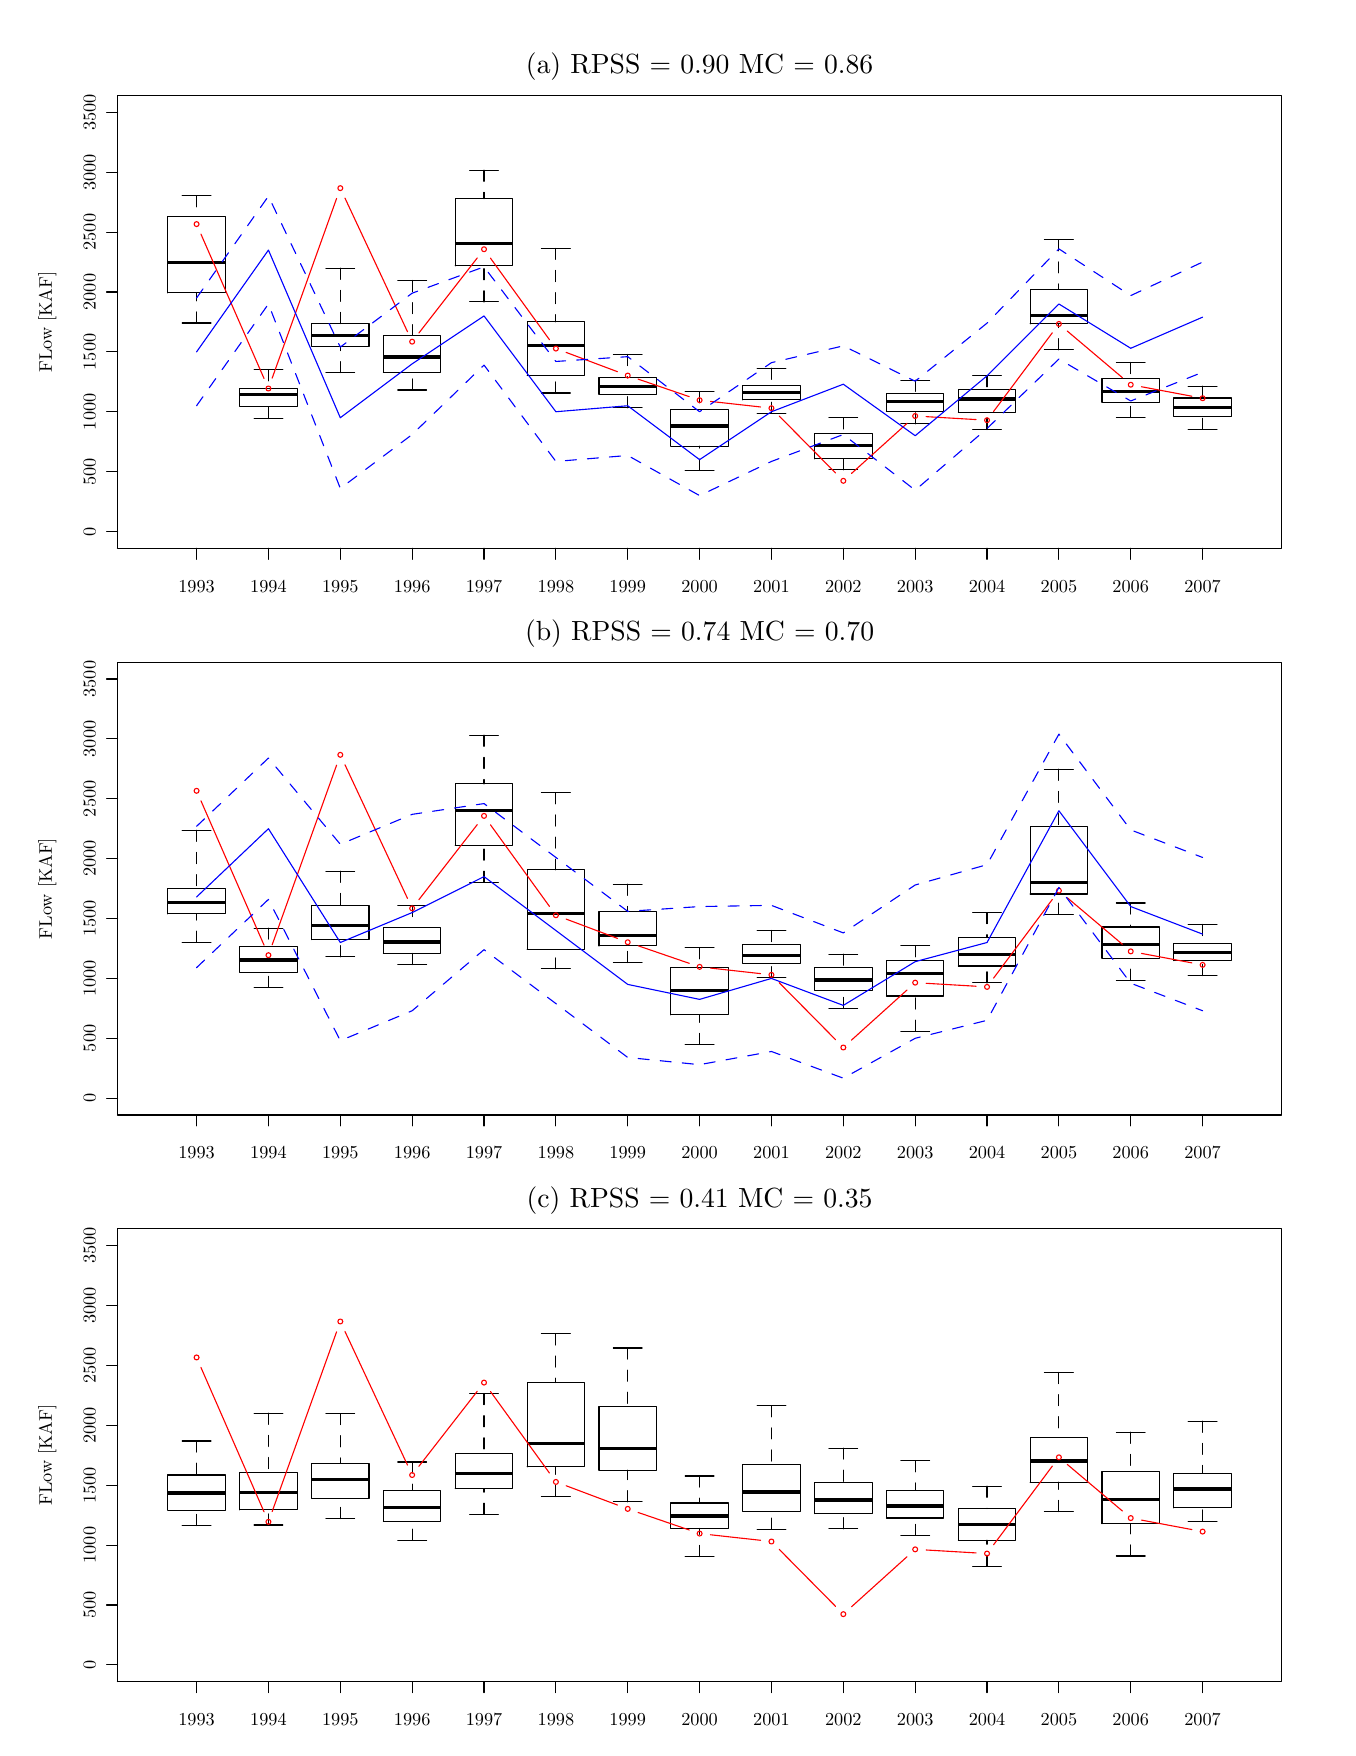
\begin{tikzpicture}[x=1pt,y=1pt]
\definecolor[named]{drawColor}{rgb}{0.00,0.00,0.00}
\definecolor[named]{fillColor}{rgb}{1.00,1.00,1.00}
\fill[color=fillColor,] (0,0) rectangle (469.75,614.29);
\begin{scope}
\path[clip] ( 32.47,426.16) rectangle (453.12,589.74);
\definecolor[named]{drawColor}{rgb}{0.00,0.00,0.00}

\draw[color=drawColor,line width= 1.2pt,line join=round,fill opacity=0.00,] ( 50.65,529.53) -- ( 71.42,529.53);

\draw[color=drawColor,dash pattern=on 4pt off 4pt ,line cap=round,line join=round,fill opacity=0.00,] ( 61.03,507.57) -- ( 61.03,518.49);

\draw[color=drawColor,dash pattern=on 4pt off 4pt ,line cap=round,line join=round,fill opacity=0.00,] ( 61.03,553.53) -- ( 61.03,546.05);

\draw[color=drawColor,line cap=round,line join=round,fill opacity=0.00,] ( 55.84,507.57) -- ( 66.23,507.57);

\draw[color=drawColor,line cap=round,line join=round,fill opacity=0.00,] ( 55.84,553.53) -- ( 66.23,553.53);

\draw[color=drawColor,line cap=round,line join=round,fill opacity=0.00,] ( 50.65,518.49) --
	( 71.42,518.49) --
	( 71.42,546.05) --
	( 50.65,546.05) --
	( 50.65,518.49);

\draw[color=drawColor,line width= 1.2pt,line join=round,fill opacity=0.00,] ( 76.61,481.66) -- ( 97.39,481.66);

\draw[color=drawColor,dash pattern=on 4pt off 4pt ,line cap=round,line join=round,fill opacity=0.00,] ( 87.00,473.06) -- ( 87.00,477.45);

\draw[color=drawColor,dash pattern=on 4pt off 4pt ,line cap=round,line join=round,fill opacity=0.00,] ( 87.00,490.65) -- ( 87.00,484.04);

\draw[color=drawColor,line cap=round,line join=round,fill opacity=0.00,] ( 81.81,473.06) -- ( 92.19,473.06);

\draw[color=drawColor,line cap=round,line join=round,fill opacity=0.00,] ( 81.81,490.65) -- ( 92.19,490.65);

\draw[color=drawColor,line cap=round,line join=round,fill opacity=0.00,] ( 76.61,477.45) --
	( 97.39,477.45) --
	( 97.39,484.04) --
	( 76.61,484.04) --
	( 76.61,477.45);

\draw[color=drawColor,line width= 1.2pt,line join=round,fill opacity=0.00,] (102.58,502.96) -- (123.35,502.96);

\draw[color=drawColor,dash pattern=on 4pt off 4pt ,line cap=round,line join=round,fill opacity=0.00,] (112.97,489.62) -- (112.97,499.12);

\draw[color=drawColor,dash pattern=on 4pt off 4pt ,line cap=round,line join=round,fill opacity=0.00,] (112.97,527.36) -- (112.97,507.26);

\draw[color=drawColor,line cap=round,line join=round,fill opacity=0.00,] (107.77,489.62) -- (118.16,489.62);

\draw[color=drawColor,line cap=round,line join=round,fill opacity=0.00,] (107.77,527.36) -- (118.16,527.36);

\draw[color=drawColor,line cap=round,line join=round,fill opacity=0.00,] (102.58,499.12) --
	(123.35,499.12) --
	(123.35,507.26) --
	(102.58,507.26) --
	(102.58,499.12);

\draw[color=drawColor,line width= 1.2pt,line join=round,fill opacity=0.00,] (128.55,495.30) -- (149.32,495.30);

\draw[color=drawColor,dash pattern=on 4pt off 4pt ,line cap=round,line join=round,fill opacity=0.00,] (138.93,483.36) -- (138.93,489.78);

\draw[color=drawColor,dash pattern=on 4pt off 4pt ,line cap=round,line join=round,fill opacity=0.00,] (138.93,522.95) -- (138.93,503.11);

\draw[color=drawColor,line cap=round,line join=round,fill opacity=0.00,] (133.74,483.36) -- (144.13,483.36);

\draw[color=drawColor,line cap=round,line join=round,fill opacity=0.00,] (133.74,522.95) -- (144.13,522.95);

\draw[color=drawColor,line cap=round,line join=round,fill opacity=0.00,] (128.55,489.78) --
	(149.32,489.78) --
	(149.32,503.11) --
	(128.55,503.11) --
	(128.55,489.78);

\draw[color=drawColor,line width= 1.2pt,line join=round,fill opacity=0.00,] (154.51,536.29) -- (175.29,536.29);

\draw[color=drawColor,dash pattern=on 4pt off 4pt ,line cap=round,line join=round,fill opacity=0.00,] (164.90,515.18) -- (164.90,528.19);

\draw[color=drawColor,dash pattern=on 4pt off 4pt ,line cap=round,line join=round,fill opacity=0.00,] (164.90,562.77) -- (164.90,552.49);

\draw[color=drawColor,line cap=round,line join=round,fill opacity=0.00,] (159.71,515.18) -- (170.09,515.18);

\draw[color=drawColor,line cap=round,line join=round,fill opacity=0.00,] (159.71,562.77) -- (170.09,562.77);

\draw[color=drawColor,line cap=round,line join=round,fill opacity=0.00,] (154.51,528.19) --
	(175.29,528.19) --
	(175.29,552.49) --
	(154.51,552.49) --
	(154.51,528.19);

\draw[color=drawColor,line width= 1.2pt,line join=round,fill opacity=0.00,] (180.48,499.32) -- (201.25,499.32);

\draw[color=drawColor,dash pattern=on 4pt off 4pt ,line cap=round,line join=round,fill opacity=0.00,] (190.87,482.27) -- (190.87,488.55);

\draw[color=drawColor,dash pattern=on 4pt off 4pt ,line cap=round,line join=round,fill opacity=0.00,] (190.87,534.55) -- (190.87,507.99);

\draw[color=drawColor,line cap=round,line join=round,fill opacity=0.00,] (185.67,482.27) -- (196.06,482.27);

\draw[color=drawColor,line cap=round,line join=round,fill opacity=0.00,] (185.67,534.55) -- (196.06,534.55);

\draw[color=drawColor,line cap=round,line join=round,fill opacity=0.00,] (180.48,488.55) --
	(201.25,488.55) --
	(201.25,507.99) --
	(180.48,507.99) --
	(180.48,488.55);

\draw[color=drawColor,line width= 1.2pt,line join=round,fill opacity=0.00,] (206.44,484.53) -- (227.22,484.53);

\draw[color=drawColor,dash pattern=on 4pt off 4pt ,line cap=round,line join=round,fill opacity=0.00,] (216.83,476.94) -- (216.83,481.86);

\draw[color=drawColor,dash pattern=on 4pt off 4pt ,line cap=round,line join=round,fill opacity=0.00,] (216.83,496.21) -- (216.83,487.75);

\draw[color=drawColor,line cap=round,line join=round,fill opacity=0.00,] (211.64,476.94) -- (222.02,476.94);

\draw[color=drawColor,line cap=round,line join=round,fill opacity=0.00,] (211.64,496.21) -- (222.02,496.21);

\draw[color=drawColor,line cap=round,line join=round,fill opacity=0.00,] (206.44,481.86) --
	(227.22,481.86) --
	(227.22,487.75) --
	(206.44,487.75) --
	(206.44,481.86);

\draw[color=drawColor,line width= 1.2pt,line join=round,fill opacity=0.00,] (232.41,470.35) -- (253.18,470.35);

\draw[color=drawColor,dash pattern=on 4pt off 4pt ,line cap=round,line join=round,fill opacity=0.00,] (242.80,454.40) -- (242.80,463.09);

\draw[color=drawColor,dash pattern=on 4pt off 4pt ,line cap=round,line join=round,fill opacity=0.00,] (242.80,482.71) -- (242.80,476.35);

\draw[color=drawColor,line cap=round,line join=round,fill opacity=0.00,] (237.60,454.40) -- (247.99,454.40);

\draw[color=drawColor,line cap=round,line join=round,fill opacity=0.00,] (237.60,482.71) -- (247.99,482.71);

\draw[color=drawColor,line cap=round,line join=round,fill opacity=0.00,] (232.41,463.09) --
	(253.18,463.09) --
	(253.18,476.35) --
	(232.41,476.35) --
	(232.41,463.09);

\draw[color=drawColor,line width= 1.2pt,line join=round,fill opacity=0.00,] (258.38,482.52) -- (279.15,482.52);

\draw[color=drawColor,dash pattern=on 4pt off 4pt ,line cap=round,line join=round,fill opacity=0.00,] (268.76,474.92) -- (268.76,479.77);

\draw[color=drawColor,dash pattern=on 4pt off 4pt ,line cap=round,line join=round,fill opacity=0.00,] (268.76,491.23) -- (268.76,485.05);

\draw[color=drawColor,line cap=round,line join=round,fill opacity=0.00,] (263.57,474.92) -- (273.96,474.92);

\draw[color=drawColor,line cap=round,line join=round,fill opacity=0.00,] (263.57,491.23) -- (273.96,491.23);

\draw[color=drawColor,line cap=round,line join=round,fill opacity=0.00,] (258.38,479.77) --
	(279.15,479.77) --
	(279.15,485.05) --
	(258.38,485.05) --
	(258.38,479.77);

\draw[color=drawColor,line width= 1.2pt,line join=round,fill opacity=0.00,] (284.34,463.35) -- (305.12,463.35);

\draw[color=drawColor,dash pattern=on 4pt off 4pt ,line cap=round,line join=round,fill opacity=0.00,] (294.73,454.51) -- (294.73,458.51);

\draw[color=drawColor,dash pattern=on 4pt off 4pt ,line cap=round,line join=round,fill opacity=0.00,] (294.73,473.28) -- (294.73,467.51);

\draw[color=drawColor,line cap=round,line join=round,fill opacity=0.00,] (289.54,454.51) -- (299.92,454.51);

\draw[color=drawColor,line cap=round,line join=round,fill opacity=0.00,] (289.54,473.28) -- (299.92,473.28);

\draw[color=drawColor,line cap=round,line join=round,fill opacity=0.00,] (284.34,458.51) --
	(305.12,458.51) --
	(305.12,467.51) --
	(284.34,467.51) --
	(284.34,458.51);

\draw[color=drawColor,line width= 1.2pt,line join=round,fill opacity=0.00,] (310.31,479.30) -- (331.08,479.30);

\draw[color=drawColor,dash pattern=on 4pt off 4pt ,line cap=round,line join=round,fill opacity=0.00,] (320.70,471.12) -- (320.70,475.71);

\draw[color=drawColor,dash pattern=on 4pt off 4pt ,line cap=round,line join=round,fill opacity=0.00,] (320.70,486.90) -- (320.70,482.15);

\draw[color=drawColor,line cap=round,line join=round,fill opacity=0.00,] (315.50,471.12) -- (325.89,471.12);

\draw[color=drawColor,line cap=round,line join=round,fill opacity=0.00,] (315.50,486.90) -- (325.89,486.90);

\draw[color=drawColor,line cap=round,line join=round,fill opacity=0.00,] (310.31,475.71) --
	(331.08,475.71) --
	(331.08,482.15) --
	(310.31,482.15) --
	(310.31,475.71);

\draw[color=drawColor,line width= 1.2pt,line join=round,fill opacity=0.00,] (336.28,480.09) -- (357.05,480.09);

\draw[color=drawColor,dash pattern=on 4pt off 4pt ,line cap=round,line join=round,fill opacity=0.00,] (346.66,469.06) -- (346.66,475.34);

\draw[color=drawColor,dash pattern=on 4pt off 4pt ,line cap=round,line join=round,fill opacity=0.00,] (346.66,488.51) -- (346.66,483.51);

\draw[color=drawColor,line cap=round,line join=round,fill opacity=0.00,] (341.47,469.06) -- (351.86,469.06);

\draw[color=drawColor,line cap=round,line join=round,fill opacity=0.00,] (341.47,488.51) -- (351.86,488.51);

\draw[color=drawColor,line cap=round,line join=round,fill opacity=0.00,] (336.28,475.34) --
	(357.05,475.34) --
	(357.05,483.51) --
	(336.28,483.51) --
	(336.28,475.34);

\draw[color=drawColor,line width= 1.2pt,line join=round,fill opacity=0.00,] (362.24,510.18) -- (383.01,510.18);

\draw[color=drawColor,dash pattern=on 4pt off 4pt ,line cap=round,line join=round,fill opacity=0.00,] (372.63,497.87) -- (372.63,507.25);

\draw[color=drawColor,dash pattern=on 4pt off 4pt ,line cap=round,line join=round,fill opacity=0.00,] (372.63,537.66) -- (372.63,519.80);

\draw[color=drawColor,line cap=round,line join=round,fill opacity=0.00,] (367.43,497.87) -- (377.82,497.87);

\draw[color=drawColor,line cap=round,line join=round,fill opacity=0.00,] (367.43,537.66) -- (377.82,537.66);

\draw[color=drawColor,line cap=round,line join=round,fill opacity=0.00,] (362.24,507.25) --
	(383.01,507.25) --
	(383.01,519.80) --
	(362.24,519.80) --
	(362.24,507.25);

\draw[color=drawColor,line width= 1.2pt,line join=round,fill opacity=0.00,] (388.21,482.93) -- (408.98,482.93);

\draw[color=drawColor,dash pattern=on 4pt off 4pt ,line cap=round,line join=round,fill opacity=0.00,] (398.59,473.42) -- (398.59,478.95);

\draw[color=drawColor,dash pattern=on 4pt off 4pt ,line cap=round,line join=round,fill opacity=0.00,] (398.59,493.29) -- (398.59,487.42);

\draw[color=drawColor,line cap=round,line join=round,fill opacity=0.00,] (393.40,473.42) -- (403.79,473.42);

\draw[color=drawColor,line cap=round,line join=round,fill opacity=0.00,] (393.40,493.29) -- (403.79,493.29);

\draw[color=drawColor,line cap=round,line join=round,fill opacity=0.00,] (388.21,478.95) --
	(408.98,478.95) --
	(408.98,487.42) --
	(388.21,487.42) --
	(388.21,478.95);

\draw[color=drawColor,line width= 1.2pt,line join=round,fill opacity=0.00,] (414.17,477.12) -- (434.95,477.12);

\draw[color=drawColor,dash pattern=on 4pt off 4pt ,line cap=round,line join=round,fill opacity=0.00,] (424.56,469.13) -- (424.56,473.84);

\draw[color=drawColor,dash pattern=on 4pt off 4pt ,line cap=round,line join=round,fill opacity=0.00,] (424.56,484.71) -- (424.56,480.46);

\draw[color=drawColor,line cap=round,line join=round,fill opacity=0.00,] (419.37,469.13) -- (429.75,469.13);

\draw[color=drawColor,line cap=round,line join=round,fill opacity=0.00,] (419.37,484.71) -- (429.75,484.71);

\draw[color=drawColor,line cap=round,line join=round,fill opacity=0.00,] (414.17,473.84) --
	(434.95,473.84) --
	(434.95,480.46) --
	(414.17,480.46) --
	(414.17,473.84);
\end{scope}
\begin{scope}
\path[clip] (  0.00,  0.00) rectangle (469.75,614.29);
\definecolor[named]{drawColor}{rgb}{0.00,0.00,0.00}

\draw[color=drawColor,line cap=round,line join=round,fill opacity=0.00,] ( 61.03,426.16) -- (424.56,426.16);

\draw[color=drawColor,line cap=round,line join=round,fill opacity=0.00,] ( 61.03,426.16) -- ( 61.03,422.20);

\draw[color=drawColor,line cap=round,line join=round,fill opacity=0.00,] ( 87.00,426.16) -- ( 87.00,422.20);

\draw[color=drawColor,line cap=round,line join=round,fill opacity=0.00,] (112.97,426.16) -- (112.97,422.20);

\draw[color=drawColor,line cap=round,line join=round,fill opacity=0.00,] (138.93,426.16) -- (138.93,422.20);

\draw[color=drawColor,line cap=round,line join=round,fill opacity=0.00,] (164.90,426.16) -- (164.90,422.20);

\draw[color=drawColor,line cap=round,line join=round,fill opacity=0.00,] (190.87,426.16) -- (190.87,422.20);

\draw[color=drawColor,line cap=round,line join=round,fill opacity=0.00,] (216.83,426.16) -- (216.83,422.20);

\draw[color=drawColor,line cap=round,line join=round,fill opacity=0.00,] (242.80,426.16) -- (242.80,422.20);

\draw[color=drawColor,line cap=round,line join=round,fill opacity=0.00,] (268.76,426.16) -- (268.76,422.20);

\draw[color=drawColor,line cap=round,line join=round,fill opacity=0.00,] (294.73,426.16) -- (294.73,422.20);

\draw[color=drawColor,line cap=round,line join=round,fill opacity=0.00,] (320.70,426.16) -- (320.70,422.20);

\draw[color=drawColor,line cap=round,line join=round,fill opacity=0.00,] (346.66,426.16) -- (346.66,422.20);

\draw[color=drawColor,line cap=round,line join=round,fill opacity=0.00,] (372.63,426.16) -- (372.63,422.20);

\draw[color=drawColor,line cap=round,line join=round,fill opacity=0.00,] (398.59,426.16) -- (398.59,422.20);

\draw[color=drawColor,line cap=round,line join=round,fill opacity=0.00,] (424.56,426.16) -- (424.56,422.20);

\node[color=drawColor,anchor=base,inner sep=0pt, outer sep=0pt, scale=  0.66] at ( 61.03,410.32) {1993%
};

\node[color=drawColor,anchor=base,inner sep=0pt, outer sep=0pt, scale=  0.66] at ( 87.00,410.32) {1994%
};

\node[color=drawColor,anchor=base,inner sep=0pt, outer sep=0pt, scale=  0.66] at (112.97,410.32) {1995%
};

\node[color=drawColor,anchor=base,inner sep=0pt, outer sep=0pt, scale=  0.66] at (138.93,410.32) {1996%
};

\node[color=drawColor,anchor=base,inner sep=0pt, outer sep=0pt, scale=  0.66] at (164.90,410.32) {1997%
};

\node[color=drawColor,anchor=base,inner sep=0pt, outer sep=0pt, scale=  0.66] at (190.87,410.32) {1998%
};

\node[color=drawColor,anchor=base,inner sep=0pt, outer sep=0pt, scale=  0.66] at (216.83,410.32) {1999%
};

\node[color=drawColor,anchor=base,inner sep=0pt, outer sep=0pt, scale=  0.66] at (242.80,410.32) {2000%
};

\node[color=drawColor,anchor=base,inner sep=0pt, outer sep=0pt, scale=  0.66] at (268.76,410.32) {2001%
};

\node[color=drawColor,anchor=base,inner sep=0pt, outer sep=0pt, scale=  0.66] at (294.73,410.32) {2002%
};

\node[color=drawColor,anchor=base,inner sep=0pt, outer sep=0pt, scale=  0.66] at (320.70,410.32) {2003%
};

\node[color=drawColor,anchor=base,inner sep=0pt, outer sep=0pt, scale=  0.66] at (346.66,410.32) {2004%
};

\node[color=drawColor,anchor=base,inner sep=0pt, outer sep=0pt, scale=  0.66] at (372.63,410.32) {2005%
};

\node[color=drawColor,anchor=base,inner sep=0pt, outer sep=0pt, scale=  0.66] at (398.59,410.32) {2006%
};

\node[color=drawColor,anchor=base,inner sep=0pt, outer sep=0pt, scale=  0.66] at (424.56,410.32) {2007%
};

\draw[color=drawColor,line cap=round,line join=round,fill opacity=0.00,] ( 32.47,432.22) -- ( 32.47,583.68);

\draw[color=drawColor,line cap=round,line join=round,fill opacity=0.00,] ( 32.47,432.22) -- ( 28.51,432.22);

\draw[color=drawColor,line cap=round,line join=round,fill opacity=0.00,] ( 32.47,453.86) -- ( 28.51,453.86);

\draw[color=drawColor,line cap=round,line join=round,fill opacity=0.00,] ( 32.47,475.50) -- ( 28.51,475.50);

\draw[color=drawColor,line cap=round,line join=round,fill opacity=0.00,] ( 32.47,497.13) -- ( 28.51,497.13);

\draw[color=drawColor,line cap=round,line join=round,fill opacity=0.00,] ( 32.47,518.77) -- ( 28.51,518.77);

\draw[color=drawColor,line cap=round,line join=round,fill opacity=0.00,] ( 32.47,540.41) -- ( 28.51,540.41);

\draw[color=drawColor,line cap=round,line join=round,fill opacity=0.00,] ( 32.47,562.05) -- ( 28.51,562.05);

\draw[color=drawColor,line cap=round,line join=round,fill opacity=0.00,] ( 32.47,583.68) -- ( 28.51,583.68);

\node[rotate= 90.00,color=drawColor,anchor=base,inner sep=0pt, outer sep=0pt, scale=  0.66] at ( 24.55,432.22) {0%
};

\node[rotate= 90.00,color=drawColor,anchor=base,inner sep=0pt, outer sep=0pt, scale=  0.66] at ( 24.55,453.86) {500%
};

\node[rotate= 90.00,color=drawColor,anchor=base,inner sep=0pt, outer sep=0pt, scale=  0.66] at ( 24.55,475.50) {1000%
};

\node[rotate= 90.00,color=drawColor,anchor=base,inner sep=0pt, outer sep=0pt, scale=  0.66] at ( 24.55,497.13) {1500%
};

\node[rotate= 90.00,color=drawColor,anchor=base,inner sep=0pt, outer sep=0pt, scale=  0.66] at ( 24.55,518.77) {2000%
};

\node[rotate= 90.00,color=drawColor,anchor=base,inner sep=0pt, outer sep=0pt, scale=  0.66] at ( 24.55,540.41) {2500%
};

\node[rotate= 90.00,color=drawColor,anchor=base,inner sep=0pt, outer sep=0pt, scale=  0.66] at ( 24.55,562.05) {3000%
};

\node[rotate= 90.00,color=drawColor,anchor=base,inner sep=0pt, outer sep=0pt, scale=  0.66] at ( 24.55,583.68) {3500%
};
\end{scope}
\begin{scope}
\path[clip] (  0.00,409.53) rectangle (469.75,614.29);
\definecolor[named]{drawColor}{rgb}{0.00,0.00,0.00}

\node[rotate= 90.00,color=drawColor,anchor=base,inner sep=0pt, outer sep=0pt, scale=  0.66] at (  8.71,507.95) {FLow [KAF]%
};
\end{scope}
\begin{scope}
\path[clip] (  0.00,  0.00) rectangle (469.75,614.29);
\definecolor[named]{drawColor}{rgb}{0.00,0.00,0.00}

\draw[color=drawColor,line cap=round,line join=round,fill opacity=0.00,] ( 32.47,426.16) --
	(453.12,426.16) --
	(453.12,589.74) --
	( 32.47,589.74) --
	( 32.47,426.16);
\end{scope}
\begin{scope}
\path[clip] ( 32.47,426.16) rectangle (453.12,589.74);
\definecolor[named]{drawColor}{rgb}{1.00,0.00,0.00}

\draw[color=drawColor,line cap=round,line join=round,fill opacity=0.00,] ( 62.62,539.67) -- ( 85.41,487.52);

\draw[color=drawColor,line cap=round,line join=round,fill opacity=0.00,] ( 88.34,487.62) -- (111.63,552.57);

\draw[color=drawColor,line cap=round,line join=round,fill opacity=0.00,] (114.65,552.71) -- (137.25,504.41);

\draw[color=drawColor,line cap=round,line join=round,fill opacity=0.00,] (141.36,503.95) -- (162.47,531.09);

\draw[color=drawColor,line cap=round,line join=round,fill opacity=0.00,] (167.22,531.01) -- (188.54,501.54);

\draw[color=drawColor,line cap=round,line join=round,fill opacity=0.00,] (194.57,496.94) -- (213.12,489.97);

\draw[color=drawColor,line cap=round,line join=round,fill opacity=0.00,] (220.58,487.29) -- (239.05,480.96);

\draw[color=drawColor,line cap=round,line join=round,fill opacity=0.00,] (246.73,479.23) -- (264.83,477.23);

\draw[color=drawColor,line cap=round,line join=round,fill opacity=0.00,] (271.55,473.97) -- (291.94,453.35);

\draw[color=drawColor,line cap=round,line join=round,fill opacity=0.00,] (297.67,453.19) -- (317.76,471.31);

\draw[color=drawColor,line cap=round,line join=round,fill opacity=0.00,] (324.65,473.73) -- (342.71,472.67);

\draw[color=drawColor,line cap=round,line join=round,fill opacity=0.00,] (349.03,475.61) -- (370.26,504.05);

\draw[color=drawColor,line cap=round,line join=round,fill opacity=0.00,] (375.65,504.66) -- (395.57,487.82);

\draw[color=drawColor,line cap=round,line join=round,fill opacity=0.00,] (402.49,484.53) -- (420.67,481.11);

\draw[color=drawColor,line cap=round,line join=round,fill opacity=0.00,] ( 61.03,543.30) circle (  0.89);

\draw[color=drawColor,line cap=round,line join=round,fill opacity=0.00,] ( 87.00,483.90) circle (  0.89);

\draw[color=drawColor,line cap=round,line join=round,fill opacity=0.00,] (112.97,556.30) circle (  0.89);

\draw[color=drawColor,line cap=round,line join=round,fill opacity=0.00,] (138.93,500.82) circle (  0.89);

\draw[color=drawColor,line cap=round,line join=round,fill opacity=0.00,] (164.90,534.22) circle (  0.89);

\draw[color=drawColor,line cap=round,line join=round,fill opacity=0.00,] (190.87,498.33) circle (  0.89);

\draw[color=drawColor,line cap=round,line join=round,fill opacity=0.00,] (216.83,488.58) circle (  0.89);

\draw[color=drawColor,line cap=round,line join=round,fill opacity=0.00,] (242.80,479.67) circle (  0.89);

\draw[color=drawColor,line cap=round,line join=round,fill opacity=0.00,] (268.76,476.79) circle (  0.89);

\draw[color=drawColor,line cap=round,line join=round,fill opacity=0.00,] (294.73,450.54) circle (  0.89);

\draw[color=drawColor,line cap=round,line join=round,fill opacity=0.00,] (320.70,473.96) circle (  0.89);

\draw[color=drawColor,line cap=round,line join=round,fill opacity=0.00,] (346.66,472.44) circle (  0.89);

\draw[color=drawColor,line cap=round,line join=round,fill opacity=0.00,] (372.63,507.22) circle (  0.89);

\draw[color=drawColor,line cap=round,line join=round,fill opacity=0.00,] (398.59,485.26) circle (  0.89);

\draw[color=drawColor,line cap=round,line join=round,fill opacity=0.00,] (424.56,480.38) circle (  0.89);
\definecolor[named]{drawColor}{rgb}{0.00,0.00,1.00}

\draw[color=drawColor,line cap=round,line join=round,fill opacity=0.00,] ( 61.03,497.13) --
	( 87.00,533.92) --
	(112.97,473.33) --
	(138.93,492.81) --
	(164.90,510.12) --
	(190.87,475.50) --
	(216.83,477.66) --
	(242.80,458.19) --
	(268.76,475.50) --
	(294.73,485.45) --
	(320.70,466.84) --
	(346.66,488.48) --
	(372.63,514.44) --
	(398.59,498.43) --
	(424.56,509.68);

\draw[color=drawColor,dash pattern=on 4pt off 4pt ,line cap=round,line join=round,fill opacity=0.00,] ( 61.03,477.66) --
	( 87.00,514.44) --
	(112.97,447.80) --
	(138.93,467.27) --
	(164.90,492.37) --
	(190.87,457.54) --
	(216.83,459.70) --
	(242.80,445.20) --
	(268.76,457.54) --
	(294.73,467.27) --
	(320.70,447.15) --
	(346.66,469.44) --
	(372.63,494.54) --
	(398.59,479.39) --
	(424.56,489.78);

\draw[color=drawColor,dash pattern=on 4pt off 4pt ,line cap=round,line join=round,fill opacity=0.00,] ( 61.03,516.61) --
	( 87.00,553.39) --
	(112.97,498.86) --
	(138.93,518.34) --
	(164.90,527.86) --
	(190.87,493.67) --
	(216.83,495.40) --
	(242.80,475.50) --
	(268.76,493.24) --
	(294.73,499.30) --
	(320.70,486.53) --
	(346.66,507.52) --
	(372.63,534.35) --
	(398.59,517.47) --
	(424.56,529.59);
\end{scope}
\begin{scope}
\path[clip] (  0.00,  0.00) rectangle (469.75,614.29);
\definecolor[named]{drawColor}{rgb}{0.00,0.00,0.00}

\node[color=drawColor,anchor=base,inner sep=0pt, outer sep=0pt, scale=  1.00] at (242.80,597.66) {(a) RPSS = 0.90 MC = 0.86%
};
\end{scope}
\begin{scope}
\path[clip] ( 32.47,221.40) rectangle (453.12,384.98);
\end{scope}
\begin{scope}
\path[clip] ( 32.47,221.40) rectangle (453.12,384.98);
\definecolor[named]{drawColor}{rgb}{0.00,0.00,0.00}

\draw[color=drawColor,line width= 1.2pt,line join=round,fill opacity=0.00,] ( 50.65,298.15) -- ( 71.42,298.15);

\draw[color=drawColor,dash pattern=on 4pt off 4pt ,line cap=round,line join=round,fill opacity=0.00,] ( 61.03,283.82) -- ( 61.03,294.06);

\draw[color=drawColor,dash pattern=on 4pt off 4pt ,line cap=round,line join=round,fill opacity=0.00,] ( 61.03,324.26) -- ( 61.03,303.36);

\draw[color=drawColor,line cap=round,line join=round,fill opacity=0.00,] ( 55.84,283.82) -- ( 66.23,283.82);

\draw[color=drawColor,line cap=round,line join=round,fill opacity=0.00,] ( 55.84,324.26) -- ( 66.23,324.26);

\draw[color=drawColor,line cap=round,line join=round,fill opacity=0.00,] ( 50.65,294.06) --
	( 71.42,294.06) --
	( 71.42,303.36) --
	( 50.65,303.36) --
	( 50.65,294.06);

\draw[color=drawColor,line width= 1.2pt,line join=round,fill opacity=0.00,] ( 76.61,277.37) -- ( 97.39,277.37);

\draw[color=drawColor,dash pattern=on 4pt off 4pt ,line cap=round,line join=round,fill opacity=0.00,] ( 87.00,267.50) -- ( 87.00,272.95);

\draw[color=drawColor,dash pattern=on 4pt off 4pt ,line cap=round,line join=round,fill opacity=0.00,] ( 87.00,288.92) -- ( 87.00,282.24);

\draw[color=drawColor,line cap=round,line join=round,fill opacity=0.00,] ( 81.81,267.50) -- ( 92.19,267.50);

\draw[color=drawColor,line cap=round,line join=round,fill opacity=0.00,] ( 81.81,288.92) -- ( 92.19,288.92);

\draw[color=drawColor,line cap=round,line join=round,fill opacity=0.00,] ( 76.61,272.95) --
	( 97.39,272.95) --
	( 97.39,282.24) --
	( 76.61,282.24) --
	( 76.61,272.95);

\draw[color=drawColor,line width= 1.2pt,line join=round,fill opacity=0.00,] (102.58,289.95) -- (123.35,289.95);

\draw[color=drawColor,dash pattern=on 4pt off 4pt ,line cap=round,line join=round,fill opacity=0.00,] (112.97,278.56) -- (112.97,284.79);

\draw[color=drawColor,dash pattern=on 4pt off 4pt ,line cap=round,line join=round,fill opacity=0.00,] (112.97,309.45) -- (112.97,297.21);

\draw[color=drawColor,line cap=round,line join=round,fill opacity=0.00,] (107.77,278.56) -- (118.16,278.56);

\draw[color=drawColor,line cap=round,line join=round,fill opacity=0.00,] (107.77,309.45) -- (118.16,309.45);

\draw[color=drawColor,line cap=round,line join=round,fill opacity=0.00,] (102.58,284.79) --
	(123.35,284.79) --
	(123.35,297.21) --
	(102.58,297.21) --
	(102.58,284.79);

\draw[color=drawColor,line width= 1.2pt,line join=round,fill opacity=0.00,] (128.55,283.86) -- (149.32,283.86);

\draw[color=drawColor,dash pattern=on 4pt off 4pt ,line cap=round,line join=round,fill opacity=0.00,] (138.93,275.74) -- (138.93,279.77);

\draw[color=drawColor,dash pattern=on 4pt off 4pt ,line cap=round,line join=round,fill opacity=0.00,] (138.93,297.11) -- (138.93,289.22);

\draw[color=drawColor,line cap=round,line join=round,fill opacity=0.00,] (133.74,275.74) -- (144.13,275.74);

\draw[color=drawColor,line cap=round,line join=round,fill opacity=0.00,] (133.74,297.11) -- (144.13,297.11);

\draw[color=drawColor,line cap=round,line join=round,fill opacity=0.00,] (128.55,279.77) --
	(149.32,279.77) --
	(149.32,289.22) --
	(128.55,289.22) --
	(128.55,279.77);

\draw[color=drawColor,line width= 1.2pt,line join=round,fill opacity=0.00,] (154.51,331.49) -- (175.29,331.49);

\draw[color=drawColor,dash pattern=on 4pt off 4pt ,line cap=round,line join=round,fill opacity=0.00,] (164.90,305.46) -- (164.90,318.81);

\draw[color=drawColor,dash pattern=on 4pt off 4pt ,line cap=round,line join=round,fill opacity=0.00,] (164.90,358.60) -- (164.90,341.04);

\draw[color=drawColor,line cap=round,line join=round,fill opacity=0.00,] (159.71,305.46) -- (170.09,305.46);

\draw[color=drawColor,line cap=round,line join=round,fill opacity=0.00,] (159.71,358.60) -- (170.09,358.60);

\draw[color=drawColor,line cap=round,line join=round,fill opacity=0.00,] (154.51,318.81) --
	(175.29,318.81) --
	(175.29,341.04) --
	(154.51,341.04) --
	(154.51,318.81);

\draw[color=drawColor,line width= 1.2pt,line join=round,fill opacity=0.00,] (180.48,294.24) -- (201.25,294.24);

\draw[color=drawColor,dash pattern=on 4pt off 4pt ,line cap=round,line join=round,fill opacity=0.00,] (190.87,274.18) -- (190.87,281.21);

\draw[color=drawColor,dash pattern=on 4pt off 4pt ,line cap=round,line join=round,fill opacity=0.00,] (190.87,337.81) -- (190.87,309.97);

\draw[color=drawColor,line cap=round,line join=round,fill opacity=0.00,] (185.67,274.18) -- (196.06,274.18);

\draw[color=drawColor,line cap=round,line join=round,fill opacity=0.00,] (185.67,337.81) -- (196.06,337.81);

\draw[color=drawColor,line cap=round,line join=round,fill opacity=0.00,] (180.48,281.21) --
	(201.25,281.21) --
	(201.25,309.97) --
	(180.48,309.97) --
	(180.48,281.21);

\draw[color=drawColor,line width= 1.2pt,line join=round,fill opacity=0.00,] (206.44,286.14) -- (227.22,286.14);

\draw[color=drawColor,dash pattern=on 4pt off 4pt ,line cap=round,line join=round,fill opacity=0.00,] (216.83,276.46) -- (216.83,282.49);

\draw[color=drawColor,dash pattern=on 4pt off 4pt ,line cap=round,line join=round,fill opacity=0.00,] (216.83,304.77) -- (216.83,294.85);

\draw[color=drawColor,line cap=round,line join=round,fill opacity=0.00,] (211.64,276.46) -- (222.02,276.46);

\draw[color=drawColor,line cap=round,line join=round,fill opacity=0.00,] (211.64,304.77) -- (222.02,304.77);

\draw[color=drawColor,line cap=round,line join=round,fill opacity=0.00,] (206.44,282.49) --
	(227.22,282.49) --
	(227.22,294.85) --
	(206.44,294.85) --
	(206.44,282.49);

\draw[color=drawColor,line width= 1.2pt,line join=round,fill opacity=0.00,] (232.41,266.48) -- (253.18,266.48);

\draw[color=drawColor,dash pattern=on 4pt off 4pt ,line cap=round,line join=round,fill opacity=0.00,] (242.80,246.90) -- (242.80,257.59);

\draw[color=drawColor,dash pattern=on 4pt off 4pt ,line cap=round,line join=round,fill opacity=0.00,] (242.80,281.84) -- (242.80,274.79);

\draw[color=drawColor,line cap=round,line join=round,fill opacity=0.00,] (237.60,246.90) -- (247.99,246.90);

\draw[color=drawColor,line cap=round,line join=round,fill opacity=0.00,] (237.60,281.84) -- (247.99,281.84);

\draw[color=drawColor,line cap=round,line join=round,fill opacity=0.00,] (232.41,257.59) --
	(253.18,257.59) --
	(253.18,274.79) --
	(232.41,274.79) --
	(232.41,257.59);

\draw[color=drawColor,line width= 1.2pt,line join=round,fill opacity=0.00,] (258.38,279.04) -- (279.15,279.04);

\draw[color=drawColor,dash pattern=on 4pt off 4pt ,line cap=round,line join=round,fill opacity=0.00,] (268.76,270.99) -- (268.76,276.27);

\draw[color=drawColor,dash pattern=on 4pt off 4pt ,line cap=round,line join=round,fill opacity=0.00,] (268.76,288.07) -- (268.76,282.96);

\draw[color=drawColor,line cap=round,line join=round,fill opacity=0.00,] (263.57,270.99) -- (273.96,270.99);

\draw[color=drawColor,line cap=round,line join=round,fill opacity=0.00,] (263.57,288.07) -- (273.96,288.07);

\draw[color=drawColor,line cap=round,line join=round,fill opacity=0.00,] (258.38,276.27) --
	(279.15,276.27) --
	(279.15,282.96) --
	(258.38,282.96) --
	(258.38,276.27);

\draw[color=drawColor,line width= 1.2pt,line join=round,fill opacity=0.00,] (284.34,270.18) -- (305.12,270.18);

\draw[color=drawColor,dash pattern=on 4pt off 4pt ,line cap=round,line join=round,fill opacity=0.00,] (294.73,259.85) -- (294.73,266.49);

\draw[color=drawColor,dash pattern=on 4pt off 4pt ,line cap=round,line join=round,fill opacity=0.00,] (294.73,279.51) -- (294.73,274.64);

\draw[color=drawColor,line cap=round,line join=round,fill opacity=0.00,] (289.54,259.85) -- (299.92,259.85);

\draw[color=drawColor,line cap=round,line join=round,fill opacity=0.00,] (289.54,279.51) -- (299.92,279.51);

\draw[color=drawColor,line cap=round,line join=round,fill opacity=0.00,] (284.34,266.49) --
	(305.12,266.49) --
	(305.12,274.64) --
	(284.34,274.64) --
	(284.34,266.49);

\draw[color=drawColor,line width= 1.2pt,line join=round,fill opacity=0.00,] (310.31,272.61) -- (331.08,272.61);

\draw[color=drawColor,dash pattern=on 4pt off 4pt ,line cap=round,line join=round,fill opacity=0.00,] (320.70,251.67) -- (320.70,264.39);

\draw[color=drawColor,dash pattern=on 4pt off 4pt ,line cap=round,line join=round,fill opacity=0.00,] (320.70,282.51) -- (320.70,277.36);

\draw[color=drawColor,line cap=round,line join=round,fill opacity=0.00,] (315.50,251.67) -- (325.89,251.67);

\draw[color=drawColor,line cap=round,line join=round,fill opacity=0.00,] (315.50,282.51) -- (325.89,282.51);

\draw[color=drawColor,line cap=round,line join=round,fill opacity=0.00,] (310.31,264.39) --
	(331.08,264.39) --
	(331.08,277.36) --
	(310.31,277.36) --
	(310.31,264.39);

\draw[color=drawColor,line width= 1.2pt,line join=round,fill opacity=0.00,] (336.28,279.31) -- (357.05,279.31);

\draw[color=drawColor,dash pattern=on 4pt off 4pt ,line cap=round,line join=round,fill opacity=0.00,] (346.66,269.12) -- (346.66,275.22);

\draw[color=drawColor,dash pattern=on 4pt off 4pt ,line cap=round,line join=round,fill opacity=0.00,] (346.66,294.52) -- (346.66,285.53);

\draw[color=drawColor,line cap=round,line join=round,fill opacity=0.00,] (341.47,269.12) -- (351.86,269.12);

\draw[color=drawColor,line cap=round,line join=round,fill opacity=0.00,] (341.47,294.52) -- (351.86,294.52);

\draw[color=drawColor,line cap=round,line join=round,fill opacity=0.00,] (336.28,275.22) --
	(357.05,275.22) --
	(357.05,285.53) --
	(336.28,285.53) --
	(336.28,275.22);

\draw[color=drawColor,line width= 1.2pt,line join=round,fill opacity=0.00,] (362.24,305.45) -- (383.01,305.45);

\draw[color=drawColor,dash pattern=on 4pt off 4pt ,line cap=round,line join=round,fill opacity=0.00,] (372.63,293.96) -- (372.63,301.25);

\draw[color=drawColor,dash pattern=on 4pt off 4pt ,line cap=round,line join=round,fill opacity=0.00,] (372.63,346.32) -- (372.63,325.78);

\draw[color=drawColor,line cap=round,line join=round,fill opacity=0.00,] (367.43,293.96) -- (377.82,293.96);

\draw[color=drawColor,line cap=round,line join=round,fill opacity=0.00,] (367.43,346.32) -- (377.82,346.32);

\draw[color=drawColor,line cap=round,line join=round,fill opacity=0.00,] (362.24,301.25) --
	(383.01,301.25) --
	(383.01,325.78) --
	(362.24,325.78) --
	(362.24,301.25);

\draw[color=drawColor,line width= 1.2pt,line join=round,fill opacity=0.00,] (388.21,283.08) -- (408.98,283.08);

\draw[color=drawColor,dash pattern=on 4pt off 4pt ,line cap=round,line join=round,fill opacity=0.00,] (398.59,270.09) -- (398.59,278.05);

\draw[color=drawColor,dash pattern=on 4pt off 4pt ,line cap=round,line join=round,fill opacity=0.00,] (398.59,297.99) -- (398.59,289.30);

\draw[color=drawColor,line cap=round,line join=round,fill opacity=0.00,] (393.40,270.09) -- (403.79,270.09);

\draw[color=drawColor,line cap=round,line join=round,fill opacity=0.00,] (393.40,297.99) -- (403.79,297.99);

\draw[color=drawColor,line cap=round,line join=round,fill opacity=0.00,] (388.21,278.05) --
	(408.98,278.05) --
	(408.98,289.30) --
	(388.21,289.30) --
	(388.21,278.05);

\draw[color=drawColor,line width= 1.2pt,line join=round,fill opacity=0.00,] (414.17,279.98) -- (434.95,279.98);

\draw[color=drawColor,dash pattern=on 4pt off 4pt ,line cap=round,line join=round,fill opacity=0.00,] (424.56,271.80) -- (424.56,277.21);

\draw[color=drawColor,dash pattern=on 4pt off 4pt ,line cap=round,line join=round,fill opacity=0.00,] (424.56,290.21) -- (424.56,283.39);

\draw[color=drawColor,line cap=round,line join=round,fill opacity=0.00,] (419.37,271.80) -- (429.75,271.80);

\draw[color=drawColor,line cap=round,line join=round,fill opacity=0.00,] (419.37,290.21) -- (429.75,290.21);

\draw[color=drawColor,line cap=round,line join=round,fill opacity=0.00,] (414.17,277.21) --
	(434.95,277.21) --
	(434.95,283.39) --
	(414.17,283.39) --
	(414.17,277.21);
\end{scope}
\begin{scope}
\path[clip] (  0.00,  0.00) rectangle (469.75,614.29);
\definecolor[named]{drawColor}{rgb}{0.00,0.00,0.00}

\draw[color=drawColor,line cap=round,line join=round,fill opacity=0.00,] ( 61.03,221.40) -- (424.56,221.40);

\draw[color=drawColor,line cap=round,line join=round,fill opacity=0.00,] ( 61.03,221.40) -- ( 61.03,217.44);

\draw[color=drawColor,line cap=round,line join=round,fill opacity=0.00,] ( 87.00,221.40) -- ( 87.00,217.44);

\draw[color=drawColor,line cap=round,line join=round,fill opacity=0.00,] (112.97,221.40) -- (112.97,217.44);

\draw[color=drawColor,line cap=round,line join=round,fill opacity=0.00,] (138.93,221.40) -- (138.93,217.44);

\draw[color=drawColor,line cap=round,line join=round,fill opacity=0.00,] (164.90,221.40) -- (164.90,217.44);

\draw[color=drawColor,line cap=round,line join=round,fill opacity=0.00,] (190.87,221.40) -- (190.87,217.44);

\draw[color=drawColor,line cap=round,line join=round,fill opacity=0.00,] (216.83,221.40) -- (216.83,217.44);

\draw[color=drawColor,line cap=round,line join=round,fill opacity=0.00,] (242.80,221.40) -- (242.80,217.44);

\draw[color=drawColor,line cap=round,line join=round,fill opacity=0.00,] (268.76,221.40) -- (268.76,217.44);

\draw[color=drawColor,line cap=round,line join=round,fill opacity=0.00,] (294.73,221.40) -- (294.73,217.44);

\draw[color=drawColor,line cap=round,line join=round,fill opacity=0.00,] (320.70,221.40) -- (320.70,217.44);

\draw[color=drawColor,line cap=round,line join=round,fill opacity=0.00,] (346.66,221.40) -- (346.66,217.44);

\draw[color=drawColor,line cap=round,line join=round,fill opacity=0.00,] (372.63,221.40) -- (372.63,217.44);

\draw[color=drawColor,line cap=round,line join=round,fill opacity=0.00,] (398.59,221.40) -- (398.59,217.44);

\draw[color=drawColor,line cap=round,line join=round,fill opacity=0.00,] (424.56,221.40) -- (424.56,217.44);

\node[color=drawColor,anchor=base,inner sep=0pt, outer sep=0pt, scale=  0.66] at ( 61.03,205.56) {1993%
};

\node[color=drawColor,anchor=base,inner sep=0pt, outer sep=0pt, scale=  0.66] at ( 87.00,205.56) {1994%
};

\node[color=drawColor,anchor=base,inner sep=0pt, outer sep=0pt, scale=  0.66] at (112.97,205.56) {1995%
};

\node[color=drawColor,anchor=base,inner sep=0pt, outer sep=0pt, scale=  0.66] at (138.93,205.56) {1996%
};

\node[color=drawColor,anchor=base,inner sep=0pt, outer sep=0pt, scale=  0.66] at (164.90,205.56) {1997%
};

\node[color=drawColor,anchor=base,inner sep=0pt, outer sep=0pt, scale=  0.66] at (190.87,205.56) {1998%
};

\node[color=drawColor,anchor=base,inner sep=0pt, outer sep=0pt, scale=  0.66] at (216.83,205.56) {1999%
};

\node[color=drawColor,anchor=base,inner sep=0pt, outer sep=0pt, scale=  0.66] at (242.80,205.56) {2000%
};

\node[color=drawColor,anchor=base,inner sep=0pt, outer sep=0pt, scale=  0.66] at (268.76,205.56) {2001%
};

\node[color=drawColor,anchor=base,inner sep=0pt, outer sep=0pt, scale=  0.66] at (294.73,205.56) {2002%
};

\node[color=drawColor,anchor=base,inner sep=0pt, outer sep=0pt, scale=  0.66] at (320.70,205.56) {2003%
};

\node[color=drawColor,anchor=base,inner sep=0pt, outer sep=0pt, scale=  0.66] at (346.66,205.56) {2004%
};

\node[color=drawColor,anchor=base,inner sep=0pt, outer sep=0pt, scale=  0.66] at (372.63,205.56) {2005%
};

\node[color=drawColor,anchor=base,inner sep=0pt, outer sep=0pt, scale=  0.66] at (398.59,205.56) {2006%
};

\node[color=drawColor,anchor=base,inner sep=0pt, outer sep=0pt, scale=  0.66] at (424.56,205.56) {2007%
};

\draw[color=drawColor,line cap=round,line join=round,fill opacity=0.00,] ( 32.47,227.46) -- ( 32.47,378.92);

\draw[color=drawColor,line cap=round,line join=round,fill opacity=0.00,] ( 32.47,227.46) -- ( 28.51,227.46);

\draw[color=drawColor,line cap=round,line join=round,fill opacity=0.00,] ( 32.47,249.09) -- ( 28.51,249.09);

\draw[color=drawColor,line cap=round,line join=round,fill opacity=0.00,] ( 32.47,270.73) -- ( 28.51,270.73);

\draw[color=drawColor,line cap=round,line join=round,fill opacity=0.00,] ( 32.47,292.37) -- ( 28.51,292.37);

\draw[color=drawColor,line cap=round,line join=round,fill opacity=0.00,] ( 32.47,314.01) -- ( 28.51,314.01);

\draw[color=drawColor,line cap=round,line join=round,fill opacity=0.00,] ( 32.47,335.64) -- ( 28.51,335.64);

\draw[color=drawColor,line cap=round,line join=round,fill opacity=0.00,] ( 32.47,357.28) -- ( 28.51,357.28);

\draw[color=drawColor,line cap=round,line join=round,fill opacity=0.00,] ( 32.47,378.92) -- ( 28.51,378.92);

\node[rotate= 90.00,color=drawColor,anchor=base,inner sep=0pt, outer sep=0pt, scale=  0.66] at ( 24.55,227.46) {0%
};

\node[rotate= 90.00,color=drawColor,anchor=base,inner sep=0pt, outer sep=0pt, scale=  0.66] at ( 24.55,249.09) {500%
};

\node[rotate= 90.00,color=drawColor,anchor=base,inner sep=0pt, outer sep=0pt, scale=  0.66] at ( 24.55,270.73) {1000%
};

\node[rotate= 90.00,color=drawColor,anchor=base,inner sep=0pt, outer sep=0pt, scale=  0.66] at ( 24.55,292.37) {1500%
};

\node[rotate= 90.00,color=drawColor,anchor=base,inner sep=0pt, outer sep=0pt, scale=  0.66] at ( 24.55,314.01) {2000%
};

\node[rotate= 90.00,color=drawColor,anchor=base,inner sep=0pt, outer sep=0pt, scale=  0.66] at ( 24.55,335.64) {2500%
};

\node[rotate= 90.00,color=drawColor,anchor=base,inner sep=0pt, outer sep=0pt, scale=  0.66] at ( 24.55,357.28) {3000%
};

\node[rotate= 90.00,color=drawColor,anchor=base,inner sep=0pt, outer sep=0pt, scale=  0.66] at ( 24.55,378.92) {3500%
};
\end{scope}
\begin{scope}
\path[clip] (  0.00,204.77) rectangle (469.75,409.53);
\definecolor[named]{drawColor}{rgb}{0.00,0.00,0.00}

\node[rotate= 90.00,color=drawColor,anchor=base,inner sep=0pt, outer sep=0pt, scale=  0.66] at (  8.71,303.19) {FLow [KAF]%
};
\end{scope}
\begin{scope}
\path[clip] (  0.00,  0.00) rectangle (469.75,614.29);
\definecolor[named]{drawColor}{rgb}{0.00,0.00,0.00}

\draw[color=drawColor,line cap=round,line join=round,fill opacity=0.00,] ( 32.47,221.40) --
	(453.12,221.40) --
	(453.12,384.98) --
	( 32.47,384.98) --
	( 32.47,221.40);
\end{scope}
\begin{scope}
\path[clip] ( 32.47,221.40) rectangle (453.12,384.98);
\definecolor[named]{drawColor}{rgb}{1.00,0.00,0.00}

\draw[color=drawColor,line cap=round,line join=round,fill opacity=0.00,] ( 62.62,334.90) -- ( 85.41,282.76);

\draw[color=drawColor,line cap=round,line join=round,fill opacity=0.00,] ( 88.34,282.86) -- (111.63,347.80);

\draw[color=drawColor,line cap=round,line join=round,fill opacity=0.00,] (114.65,347.94) -- (137.25,299.64);

\draw[color=drawColor,line cap=round,line join=round,fill opacity=0.00,] (141.36,299.18) -- (162.47,326.33);

\draw[color=drawColor,line cap=round,line join=round,fill opacity=0.00,] (167.22,326.25) -- (188.54,296.77);

\draw[color=drawColor,line cap=round,line join=round,fill opacity=0.00,] (194.57,292.17) -- (213.12,285.20);

\draw[color=drawColor,line cap=round,line join=round,fill opacity=0.00,] (220.58,282.53) -- (239.05,276.19);

\draw[color=drawColor,line cap=round,line join=round,fill opacity=0.00,] (246.73,274.47) -- (264.83,272.46);

\draw[color=drawColor,line cap=round,line join=round,fill opacity=0.00,] (271.55,269.21) -- (291.94,248.59);

\draw[color=drawColor,line cap=round,line join=round,fill opacity=0.00,] (297.67,248.43) -- (317.76,266.55);

\draw[color=drawColor,line cap=round,line join=round,fill opacity=0.00,] (324.65,268.97) -- (342.71,267.91);

\draw[color=drawColor,line cap=round,line join=round,fill opacity=0.00,] (349.03,270.85) -- (370.26,299.28);

\draw[color=drawColor,line cap=round,line join=round,fill opacity=0.00,] (375.65,299.90) -- (395.57,283.06);

\draw[color=drawColor,line cap=round,line join=round,fill opacity=0.00,] (402.49,279.77) -- (420.67,276.35);

\draw[color=drawColor,line cap=round,line join=round,fill opacity=0.00,] ( 61.03,338.53) circle (  0.89);

\draw[color=drawColor,line cap=round,line join=round,fill opacity=0.00,] ( 87.00,279.13) circle (  0.89);

\draw[color=drawColor,line cap=round,line join=round,fill opacity=0.00,] (112.97,351.53) circle (  0.89);

\draw[color=drawColor,line cap=round,line join=round,fill opacity=0.00,] (138.93,296.06) circle (  0.89);

\draw[color=drawColor,line cap=round,line join=round,fill opacity=0.00,] (164.90,329.46) circle (  0.89);

\draw[color=drawColor,line cap=round,line join=round,fill opacity=0.00,] (190.87,293.56) circle (  0.89);

\draw[color=drawColor,line cap=round,line join=round,fill opacity=0.00,] (216.83,283.81) circle (  0.89);

\draw[color=drawColor,line cap=round,line join=round,fill opacity=0.00,] (242.80,274.91) circle (  0.89);

\draw[color=drawColor,line cap=round,line join=round,fill opacity=0.00,] (268.76,272.02) circle (  0.89);

\draw[color=drawColor,line cap=round,line join=round,fill opacity=0.00,] (294.73,245.77) circle (  0.89);

\draw[color=drawColor,line cap=round,line join=round,fill opacity=0.00,] (320.70,269.20) circle (  0.89);

\draw[color=drawColor,line cap=round,line join=round,fill opacity=0.00,] (346.66,267.67) circle (  0.89);

\draw[color=drawColor,line cap=round,line join=round,fill opacity=0.00,] (372.63,302.45) circle (  0.89);

\draw[color=drawColor,line cap=round,line join=round,fill opacity=0.00,] (398.59,280.50) circle (  0.89);

\draw[color=drawColor,line cap=round,line join=round,fill opacity=0.00,] (424.56,275.62) circle (  0.89);
\definecolor[named]{drawColor}{rgb}{0.00,0.00,1.00}

\draw[color=drawColor,line cap=round,line join=round,fill opacity=0.00,] ( 61.03,300.16) --
	( 87.00,324.83) --
	(112.97,283.71) --
	(138.93,294.53) --
	(164.90,307.52) --
	(190.87,288.04) --
	(216.83,268.57) --
	(242.80,263.16) --
	(268.76,270.73) --
	(294.73,260.99) --
	(320.70,276.79) --
	(346.66,283.71) --
	(372.63,331.32) --
	(398.59,296.70) --
	(424.56,286.74);

\draw[color=drawColor,dash pattern=on 4pt off 4pt ,line cap=round,line join=round,fill opacity=0.00,] ( 61.03,274.63) --
	( 87.00,299.29) --
	(112.97,248.23) --
	(138.93,259.05) --
	(164.90,281.12) --
	(190.87,261.64) --
	(216.83,242.17) --
	(242.80,239.57) --
	(268.76,244.33) --
	(294.73,234.68) --
	(320.70,249.09) --
	(346.66,255.58) --
	(372.63,303.62) --
	(398.59,269.00) --
	(424.56,259.05);

\draw[color=drawColor,dash pattern=on 4pt off 4pt ,line cap=round,line join=round,fill opacity=0.00,] ( 61.03,325.69) --
	( 87.00,350.36) --
	(112.97,319.20) --
	(138.93,330.02) --
	(164.90,333.91) --
	(190.87,314.44) --
	(216.83,294.97) --
	(242.80,296.70) --
	(268.76,297.13) --
	(294.73,287.18) --
	(320.70,304.49) --
	(346.66,311.84) --
	(372.63,359.01) --
	(398.59,324.39) --
	(424.56,314.44);
\end{scope}
\begin{scope}
\path[clip] (  0.00,  0.00) rectangle (469.75,614.29);
\definecolor[named]{drawColor}{rgb}{0.00,0.00,0.00}

\node[color=drawColor,anchor=base,inner sep=0pt, outer sep=0pt, scale=  1.00] at (242.80,392.90) {(b) RPSS = 0.74 MC = 0.70%
};
\end{scope}
\begin{scope}
\path[clip] ( 32.47, 16.63) rectangle (453.12,180.21);
\end{scope}
\begin{scope}
\path[clip] ( 32.47, 16.63) rectangle (453.12,180.21);
\definecolor[named]{drawColor}{rgb}{0.00,0.00,0.00}

\draw[color=drawColor,line width= 1.2pt,line join=round,fill opacity=0.00,] ( 50.65, 84.79) -- ( 71.42, 84.79);

\draw[color=drawColor,dash pattern=on 4pt off 4pt ,line cap=round,line join=round,fill opacity=0.00,] ( 61.03, 73.03) -- ( 61.03, 78.59);

\draw[color=drawColor,dash pattern=on 4pt off 4pt ,line cap=round,line join=round,fill opacity=0.00,] ( 61.03,103.60) -- ( 61.03, 91.31);

\draw[color=drawColor,line cap=round,line join=round,fill opacity=0.00,] ( 55.84, 73.03) -- ( 66.23, 73.03);

\draw[color=drawColor,line cap=round,line join=round,fill opacity=0.00,] ( 55.84,103.60) -- ( 66.23,103.60);

\draw[color=drawColor,line cap=round,line join=round,fill opacity=0.00,] ( 50.65, 78.59) --
	( 71.42, 78.59) --
	( 71.42, 91.31) --
	( 50.65, 91.31) --
	( 50.65, 78.59);

\draw[color=drawColor,line width= 1.2pt,line join=round,fill opacity=0.00,] ( 76.61, 84.96) -- ( 97.39, 84.96);

\draw[color=drawColor,dash pattern=on 4pt off 4pt ,line cap=round,line join=round,fill opacity=0.00,] ( 87.00, 73.23) -- ( 87.00, 78.72);

\draw[color=drawColor,dash pattern=on 4pt off 4pt ,line cap=round,line join=round,fill opacity=0.00,] ( 87.00,113.61) -- ( 87.00, 92.26);

\draw[color=drawColor,line cap=round,line join=round,fill opacity=0.00,] ( 81.81, 73.23) -- ( 92.19, 73.23);

\draw[color=drawColor,line cap=round,line join=round,fill opacity=0.00,] ( 81.81,113.61) -- ( 92.19,113.61);

\draw[color=drawColor,line cap=round,line join=round,fill opacity=0.00,] ( 76.61, 78.72) --
	( 97.39, 78.72) --
	( 97.39, 92.26) --
	( 76.61, 92.26) --
	( 76.61, 78.72);

\draw[color=drawColor,line width= 1.2pt,line join=round,fill opacity=0.00,] (102.58, 89.57) -- (123.35, 89.57);

\draw[color=drawColor,dash pattern=on 4pt off 4pt ,line cap=round,line join=round,fill opacity=0.00,] (112.97, 75.55) -- (112.97, 82.84);

\draw[color=drawColor,dash pattern=on 4pt off 4pt ,line cap=round,line join=round,fill opacity=0.00,] (112.97,113.48) -- (112.97, 95.61);

\draw[color=drawColor,line cap=round,line join=round,fill opacity=0.00,] (107.77, 75.55) -- (118.16, 75.55);

\draw[color=drawColor,line cap=round,line join=round,fill opacity=0.00,] (107.77,113.48) -- (118.16,113.48);

\draw[color=drawColor,line cap=round,line join=round,fill opacity=0.00,] (102.58, 82.84) --
	(123.35, 82.84) --
	(123.35, 95.61) --
	(102.58, 95.61) --
	(102.58, 82.84);

\draw[color=drawColor,line width= 1.2pt,line join=round,fill opacity=0.00,] (128.55, 79.60) -- (149.32, 79.60);

\draw[color=drawColor,dash pattern=on 4pt off 4pt ,line cap=round,line join=round,fill opacity=0.00,] (138.93, 67.74) -- (138.93, 74.64);

\draw[color=drawColor,dash pattern=on 4pt off 4pt ,line cap=round,line join=round,fill opacity=0.00,] (138.93, 95.99) -- (138.93, 85.74);

\draw[color=drawColor,line cap=round,line join=round,fill opacity=0.00,] (133.74, 67.74) -- (144.13, 67.74);

\draw[color=drawColor,line cap=round,line join=round,fill opacity=0.00,] (133.74, 95.99) -- (144.13, 95.99);

\draw[color=drawColor,line cap=round,line join=round,fill opacity=0.00,] (128.55, 74.64) --
	(149.32, 74.64) --
	(149.32, 85.74) --
	(128.55, 85.74) --
	(128.55, 74.64);

\draw[color=drawColor,line width= 1.2pt,line join=round,fill opacity=0.00,] (154.51, 91.94) -- (175.29, 91.94);

\draw[color=drawColor,dash pattern=on 4pt off 4pt ,line cap=round,line join=round,fill opacity=0.00,] (164.90, 77.10) -- (164.90, 86.38);

\draw[color=drawColor,dash pattern=on 4pt off 4pt ,line cap=round,line join=round,fill opacity=0.00,] (164.90,120.73) -- (164.90, 98.93);

\draw[color=drawColor,line cap=round,line join=round,fill opacity=0.00,] (159.71, 77.10) -- (170.09, 77.10);

\draw[color=drawColor,line cap=round,line join=round,fill opacity=0.00,] (159.71,120.73) -- (170.09,120.73);

\draw[color=drawColor,line cap=round,line join=round,fill opacity=0.00,] (154.51, 86.38) --
	(175.29, 86.38) --
	(175.29, 98.93) --
	(154.51, 98.93) --
	(154.51, 86.38);

\draw[color=drawColor,line width= 1.2pt,line join=round,fill opacity=0.00,] (180.48,102.80) -- (201.25,102.80);

\draw[color=drawColor,dash pattern=on 4pt off 4pt ,line cap=round,line join=round,fill opacity=0.00,] (190.87, 83.54) -- (190.87, 94.22);

\draw[color=drawColor,dash pattern=on 4pt off 4pt ,line cap=round,line join=round,fill opacity=0.00,] (190.87,142.28) -- (190.87,124.71);

\draw[color=drawColor,line cap=round,line join=round,fill opacity=0.00,] (185.67, 83.54) -- (196.06, 83.54);

\draw[color=drawColor,line cap=round,line join=round,fill opacity=0.00,] (185.67,142.28) -- (196.06,142.28);

\draw[color=drawColor,line cap=round,line join=round,fill opacity=0.00,] (180.48, 94.22) --
	(201.25, 94.22) --
	(201.25,124.71) --
	(180.48,124.71) --
	(180.48, 94.22);

\draw[color=drawColor,line width= 1.2pt,line join=round,fill opacity=0.00,] (206.44,100.83) -- (227.22,100.83);

\draw[color=drawColor,dash pattern=on 4pt off 4pt ,line cap=round,line join=round,fill opacity=0.00,] (216.83, 81.63) -- (216.83, 93.07);

\draw[color=drawColor,dash pattern=on 4pt off 4pt ,line cap=round,line join=round,fill opacity=0.00,] (216.83,137.19) -- (216.83,116.13);

\draw[color=drawColor,line cap=round,line join=round,fill opacity=0.00,] (211.64, 81.63) -- (222.02, 81.63);

\draw[color=drawColor,line cap=round,line join=round,fill opacity=0.00,] (211.64,137.19) -- (222.02,137.19);

\draw[color=drawColor,line cap=round,line join=round,fill opacity=0.00,] (206.44, 93.07) --
	(227.22, 93.07) --
	(227.22,116.13) --
	(206.44,116.13) --
	(206.44, 93.07);

\draw[color=drawColor,line width= 1.2pt,line join=round,fill opacity=0.00,] (232.41, 76.45) -- (253.18, 76.45);

\draw[color=drawColor,dash pattern=on 4pt off 4pt ,line cap=round,line join=round,fill opacity=0.00,] (242.80, 61.84) -- (242.80, 72.00);

\draw[color=drawColor,dash pattern=on 4pt off 4pt ,line cap=round,line join=round,fill opacity=0.00,] (242.80, 90.93) -- (242.80, 81.17);

\draw[color=drawColor,line cap=round,line join=round,fill opacity=0.00,] (237.60, 61.84) -- (247.99, 61.84);

\draw[color=drawColor,line cap=round,line join=round,fill opacity=0.00,] (237.60, 90.93) -- (247.99, 90.93);

\draw[color=drawColor,line cap=round,line join=round,fill opacity=0.00,] (232.41, 72.00) --
	(253.18, 72.00) --
	(253.18, 81.17) --
	(232.41, 81.17) --
	(232.41, 72.00);

\draw[color=drawColor,line width= 1.2pt,line join=round,fill opacity=0.00,] (258.38, 85.13) -- (279.15, 85.13);

\draw[color=drawColor,dash pattern=on 4pt off 4pt ,line cap=round,line join=round,fill opacity=0.00,] (268.76, 71.74) -- (268.76, 78.26);

\draw[color=drawColor,dash pattern=on 4pt off 4pt ,line cap=round,line join=round,fill opacity=0.00,] (268.76,116.35) -- (268.76, 95.06);

\draw[color=drawColor,line cap=round,line join=round,fill opacity=0.00,] (263.57, 71.74) -- (273.96, 71.74);

\draw[color=drawColor,line cap=round,line join=round,fill opacity=0.00,] (263.57,116.35) -- (273.96,116.35);

\draw[color=drawColor,line cap=round,line join=round,fill opacity=0.00,] (258.38, 78.26) --
	(279.15, 78.26) --
	(279.15, 95.06) --
	(258.38, 95.06) --
	(258.38, 78.26);

\draw[color=drawColor,line width= 1.2pt,line join=round,fill opacity=0.00,] (284.34, 82.22) -- (305.12, 82.22);

\draw[color=drawColor,dash pattern=on 4pt off 4pt ,line cap=round,line join=round,fill opacity=0.00,] (294.73, 71.87) -- (294.73, 77.35);

\draw[color=drawColor,dash pattern=on 4pt off 4pt ,line cap=round,line join=round,fill opacity=0.00,] (294.73,101.01) -- (294.73, 88.44);

\draw[color=drawColor,line cap=round,line join=round,fill opacity=0.00,] (289.54, 71.87) -- (299.92, 71.87);

\draw[color=drawColor,line cap=round,line join=round,fill opacity=0.00,] (289.54,101.01) -- (299.92,101.01);

\draw[color=drawColor,line cap=round,line join=round,fill opacity=0.00,] (284.34, 77.35) --
	(305.12, 77.35) --
	(305.12, 88.44) --
	(284.34, 88.44) --
	(284.34, 77.35);

\draw[color=drawColor,line width= 1.2pt,line join=round,fill opacity=0.00,] (310.31, 80.13) -- (331.08, 80.13);

\draw[color=drawColor,dash pattern=on 4pt off 4pt ,line cap=round,line join=round,fill opacity=0.00,] (320.70, 69.46) -- (320.70, 75.76);

\draw[color=drawColor,dash pattern=on 4pt off 4pt ,line cap=round,line join=round,fill opacity=0.00,] (320.70, 96.45) -- (320.70, 85.85);

\draw[color=drawColor,line cap=round,line join=round,fill opacity=0.00,] (315.50, 69.46) -- (325.89, 69.46);

\draw[color=drawColor,line cap=round,line join=round,fill opacity=0.00,] (315.50, 96.45) -- (325.89, 96.45);

\draw[color=drawColor,line cap=round,line join=round,fill opacity=0.00,] (310.31, 75.76) --
	(331.08, 75.76) --
	(331.08, 85.85) --
	(310.31, 85.85) --
	(310.31, 75.76);

\draw[color=drawColor,line width= 1.2pt,line join=round,fill opacity=0.00,] (336.28, 73.40) -- (357.05, 73.40);

\draw[color=drawColor,dash pattern=on 4pt off 4pt ,line cap=round,line join=round,fill opacity=0.00,] (346.66, 58.29) -- (346.66, 67.71);

\draw[color=drawColor,dash pattern=on 4pt off 4pt ,line cap=round,line join=round,fill opacity=0.00,] (346.66, 87.25) -- (346.66, 79.21);

\draw[color=drawColor,line cap=round,line join=round,fill opacity=0.00,] (341.47, 58.29) -- (351.86, 58.29);

\draw[color=drawColor,line cap=round,line join=round,fill opacity=0.00,] (341.47, 87.25) -- (351.86, 87.25);

\draw[color=drawColor,line cap=round,line join=round,fill opacity=0.00,] (336.28, 67.71) --
	(357.05, 67.71) --
	(357.05, 79.21) --
	(336.28, 79.21) --
	(336.28, 67.71);

\draw[color=drawColor,line width= 1.2pt,line join=round,fill opacity=0.00,] (362.24, 96.40) -- (383.01, 96.40);

\draw[color=drawColor,dash pattern=on 4pt off 4pt ,line cap=round,line join=round,fill opacity=0.00,] (372.63, 78.12) -- (372.63, 88.72);

\draw[color=drawColor,dash pattern=on 4pt off 4pt ,line cap=round,line join=round,fill opacity=0.00,] (372.63,128.35) -- (372.63,104.84);

\draw[color=drawColor,line cap=round,line join=round,fill opacity=0.00,] (367.43, 78.12) -- (377.82, 78.12);

\draw[color=drawColor,line cap=round,line join=round,fill opacity=0.00,] (367.43,128.35) -- (377.82,128.35);

\draw[color=drawColor,line cap=round,line join=round,fill opacity=0.00,] (362.24, 88.72) --
	(383.01, 88.72) --
	(383.01,104.84) --
	(362.24,104.84) --
	(362.24, 88.72);

\draw[color=drawColor,line width= 1.2pt,line join=round,fill opacity=0.00,] (388.21, 82.38) -- (408.98, 82.38);

\draw[color=drawColor,dash pattern=on 4pt off 4pt ,line cap=round,line join=round,fill opacity=0.00,] (398.59, 62.02) -- (398.59, 73.71);

\draw[color=drawColor,dash pattern=on 4pt off 4pt ,line cap=round,line join=round,fill opacity=0.00,] (398.59,106.76) -- (398.59, 92.69);

\draw[color=drawColor,line cap=round,line join=round,fill opacity=0.00,] (393.40, 62.02) -- (403.79, 62.02);

\draw[color=drawColor,line cap=round,line join=round,fill opacity=0.00,] (393.40,106.76) -- (403.79,106.76);

\draw[color=drawColor,line cap=round,line join=round,fill opacity=0.00,] (388.21, 73.71) --
	(408.98, 73.71) --
	(408.98, 92.69) --
	(388.21, 92.69) --
	(388.21, 73.71);

\draw[color=drawColor,line width= 1.2pt,line join=round,fill opacity=0.00,] (414.17, 86.25) -- (434.95, 86.25);

\draw[color=drawColor,dash pattern=on 4pt off 4pt ,line cap=round,line join=round,fill opacity=0.00,] (424.56, 74.65) -- (424.56, 79.46);

\draw[color=drawColor,dash pattern=on 4pt off 4pt ,line cap=round,line join=round,fill opacity=0.00,] (424.56,110.73) -- (424.56, 91.88);

\draw[color=drawColor,line cap=round,line join=round,fill opacity=0.00,] (419.37, 74.65) -- (429.75, 74.65);

\draw[color=drawColor,line cap=round,line join=round,fill opacity=0.00,] (419.37,110.73) -- (429.75,110.73);

\draw[color=drawColor,line cap=round,line join=round,fill opacity=0.00,] (414.17, 79.46) --
	(434.95, 79.46) --
	(434.95, 91.88) --
	(414.17, 91.88) --
	(414.17, 79.46);
\end{scope}
\begin{scope}
\path[clip] (  0.00,  0.00) rectangle (469.75,614.29);
\definecolor[named]{drawColor}{rgb}{0.00,0.00,0.00}

\draw[color=drawColor,line cap=round,line join=round,fill opacity=0.00,] ( 61.03, 16.63) -- (424.56, 16.63);

\draw[color=drawColor,line cap=round,line join=round,fill opacity=0.00,] ( 61.03, 16.63) -- ( 61.03, 12.67);

\draw[color=drawColor,line cap=round,line join=round,fill opacity=0.00,] ( 87.00, 16.63) -- ( 87.00, 12.67);

\draw[color=drawColor,line cap=round,line join=round,fill opacity=0.00,] (112.97, 16.63) -- (112.97, 12.67);

\draw[color=drawColor,line cap=round,line join=round,fill opacity=0.00,] (138.93, 16.63) -- (138.93, 12.67);

\draw[color=drawColor,line cap=round,line join=round,fill opacity=0.00,] (164.90, 16.63) -- (164.90, 12.67);

\draw[color=drawColor,line cap=round,line join=round,fill opacity=0.00,] (190.87, 16.63) -- (190.87, 12.67);

\draw[color=drawColor,line cap=round,line join=round,fill opacity=0.00,] (216.83, 16.63) -- (216.83, 12.67);

\draw[color=drawColor,line cap=round,line join=round,fill opacity=0.00,] (242.80, 16.63) -- (242.80, 12.67);

\draw[color=drawColor,line cap=round,line join=round,fill opacity=0.00,] (268.76, 16.63) -- (268.76, 12.67);

\draw[color=drawColor,line cap=round,line join=round,fill opacity=0.00,] (294.73, 16.63) -- (294.73, 12.67);

\draw[color=drawColor,line cap=round,line join=round,fill opacity=0.00,] (320.70, 16.63) -- (320.70, 12.67);

\draw[color=drawColor,line cap=round,line join=round,fill opacity=0.00,] (346.66, 16.63) -- (346.66, 12.67);

\draw[color=drawColor,line cap=round,line join=round,fill opacity=0.00,] (372.63, 16.63) -- (372.63, 12.67);

\draw[color=drawColor,line cap=round,line join=round,fill opacity=0.00,] (398.59, 16.63) -- (398.59, 12.67);

\draw[color=drawColor,line cap=round,line join=round,fill opacity=0.00,] (424.56, 16.63) -- (424.56, 12.67);

\node[color=drawColor,anchor=base,inner sep=0pt, outer sep=0pt, scale=  0.66] at ( 61.03,  0.79) {1993%
};

\node[color=drawColor,anchor=base,inner sep=0pt, outer sep=0pt, scale=  0.66] at ( 87.00,  0.79) {1994%
};

\node[color=drawColor,anchor=base,inner sep=0pt, outer sep=0pt, scale=  0.66] at (112.97,  0.79) {1995%
};

\node[color=drawColor,anchor=base,inner sep=0pt, outer sep=0pt, scale=  0.66] at (138.93,  0.79) {1996%
};

\node[color=drawColor,anchor=base,inner sep=0pt, outer sep=0pt, scale=  0.66] at (164.90,  0.79) {1997%
};

\node[color=drawColor,anchor=base,inner sep=0pt, outer sep=0pt, scale=  0.66] at (190.87,  0.79) {1998%
};

\node[color=drawColor,anchor=base,inner sep=0pt, outer sep=0pt, scale=  0.66] at (216.83,  0.79) {1999%
};

\node[color=drawColor,anchor=base,inner sep=0pt, outer sep=0pt, scale=  0.66] at (242.80,  0.79) {2000%
};

\node[color=drawColor,anchor=base,inner sep=0pt, outer sep=0pt, scale=  0.66] at (268.76,  0.79) {2001%
};

\node[color=drawColor,anchor=base,inner sep=0pt, outer sep=0pt, scale=  0.66] at (294.73,  0.79) {2002%
};

\node[color=drawColor,anchor=base,inner sep=0pt, outer sep=0pt, scale=  0.66] at (320.70,  0.79) {2003%
};

\node[color=drawColor,anchor=base,inner sep=0pt, outer sep=0pt, scale=  0.66] at (346.66,  0.79) {2004%
};

\node[color=drawColor,anchor=base,inner sep=0pt, outer sep=0pt, scale=  0.66] at (372.63,  0.79) {2005%
};

\node[color=drawColor,anchor=base,inner sep=0pt, outer sep=0pt, scale=  0.66] at (398.59,  0.79) {2006%
};

\node[color=drawColor,anchor=base,inner sep=0pt, outer sep=0pt, scale=  0.66] at (424.56,  0.79) {2007%
};

\draw[color=drawColor,line cap=round,line join=round,fill opacity=0.00,] ( 32.47, 22.69) -- ( 32.47,174.15);

\draw[color=drawColor,line cap=round,line join=round,fill opacity=0.00,] ( 32.47, 22.69) -- ( 28.51, 22.69);

\draw[color=drawColor,line cap=round,line join=round,fill opacity=0.00,] ( 32.47, 44.33) -- ( 28.51, 44.33);

\draw[color=drawColor,line cap=round,line join=round,fill opacity=0.00,] ( 32.47, 65.97) -- ( 28.51, 65.97);

\draw[color=drawColor,line cap=round,line join=round,fill opacity=0.00,] ( 32.47, 87.60) -- ( 28.51, 87.60);

\draw[color=drawColor,line cap=round,line join=round,fill opacity=0.00,] ( 32.47,109.24) -- ( 28.51,109.24);

\draw[color=drawColor,line cap=round,line join=round,fill opacity=0.00,] ( 32.47,130.88) -- ( 28.51,130.88);

\draw[color=drawColor,line cap=round,line join=round,fill opacity=0.00,] ( 32.47,152.52) -- ( 28.51,152.52);

\draw[color=drawColor,line cap=round,line join=round,fill opacity=0.00,] ( 32.47,174.15) -- ( 28.51,174.15);

\node[rotate= 90.00,color=drawColor,anchor=base,inner sep=0pt, outer sep=0pt, scale=  0.66] at ( 24.55, 22.69) {0%
};

\node[rotate= 90.00,color=drawColor,anchor=base,inner sep=0pt, outer sep=0pt, scale=  0.66] at ( 24.55, 44.33) {500%
};

\node[rotate= 90.00,color=drawColor,anchor=base,inner sep=0pt, outer sep=0pt, scale=  0.66] at ( 24.55, 65.97) {1000%
};

\node[rotate= 90.00,color=drawColor,anchor=base,inner sep=0pt, outer sep=0pt, scale=  0.66] at ( 24.55, 87.60) {1500%
};

\node[rotate= 90.00,color=drawColor,anchor=base,inner sep=0pt, outer sep=0pt, scale=  0.66] at ( 24.55,109.24) {2000%
};

\node[rotate= 90.00,color=drawColor,anchor=base,inner sep=0pt, outer sep=0pt, scale=  0.66] at ( 24.55,130.88) {2500%
};

\node[rotate= 90.00,color=drawColor,anchor=base,inner sep=0pt, outer sep=0pt, scale=  0.66] at ( 24.55,152.52) {3000%
};

\node[rotate= 90.00,color=drawColor,anchor=base,inner sep=0pt, outer sep=0pt, scale=  0.66] at ( 24.55,174.15) {3500%
};
\end{scope}
\begin{scope}
\path[clip] (  0.00,  0.00) rectangle (469.75,204.77);
\definecolor[named]{drawColor}{rgb}{0.00,0.00,0.00}

\node[rotate= 90.00,color=drawColor,anchor=base,inner sep=0pt, outer sep=0pt, scale=  0.66] at (  8.71, 98.42) {FLow [KAF]%
};
\end{scope}
\begin{scope}
\path[clip] (  0.00,  0.00) rectangle (469.75,614.29);
\definecolor[named]{drawColor}{rgb}{0.00,0.00,0.00}

\draw[color=drawColor,line cap=round,line join=round,fill opacity=0.00,] ( 32.47, 16.63) --
	(453.12, 16.63) --
	(453.12,180.21) --
	( 32.47,180.21) --
	( 32.47, 16.63);
\end{scope}
\begin{scope}
\path[clip] ( 32.47, 16.63) rectangle (453.12,180.21);
\definecolor[named]{drawColor}{rgb}{1.00,0.00,0.00}

\draw[color=drawColor,line cap=round,line join=round,fill opacity=0.00,] ( 62.62,130.14) -- ( 85.41, 77.99);

\draw[color=drawColor,line cap=round,line join=round,fill opacity=0.00,] ( 88.34, 78.09) -- (111.63,143.04);

\draw[color=drawColor,line cap=round,line join=round,fill opacity=0.00,] (114.65,143.18) -- (137.25, 94.88);

\draw[color=drawColor,line cap=round,line join=round,fill opacity=0.00,] (141.36, 94.42) -- (162.47,121.56);

\draw[color=drawColor,line cap=round,line join=round,fill opacity=0.00,] (167.22,121.48) -- (188.54, 92.01);

\draw[color=drawColor,line cap=round,line join=round,fill opacity=0.00,] (194.57, 87.41) -- (213.12, 80.44);

\draw[color=drawColor,line cap=round,line join=round,fill opacity=0.00,] (220.58, 77.76) -- (239.05, 71.43);

\draw[color=drawColor,line cap=round,line join=round,fill opacity=0.00,] (246.73, 69.70) -- (264.83, 67.70);

\draw[color=drawColor,line cap=round,line join=round,fill opacity=0.00,] (271.55, 64.44) -- (291.94, 43.82);

\draw[color=drawColor,line cap=round,line join=round,fill opacity=0.00,] (297.67, 43.66) -- (317.76, 61.78);

\draw[color=drawColor,line cap=round,line join=round,fill opacity=0.00,] (324.65, 64.20) -- (342.71, 63.14);

\draw[color=drawColor,line cap=round,line join=round,fill opacity=0.00,] (349.03, 66.08) -- (370.26, 94.52);

\draw[color=drawColor,line cap=round,line join=round,fill opacity=0.00,] (375.65, 95.13) -- (395.57, 78.29);

\draw[color=drawColor,line cap=round,line join=round,fill opacity=0.00,] (402.49, 75.00) -- (420.67, 71.58);

\draw[color=drawColor,line cap=round,line join=round,fill opacity=0.00,] ( 61.03,133.77) circle (  0.89);

\draw[color=drawColor,line cap=round,line join=round,fill opacity=0.00,] ( 87.00, 74.37) circle (  0.89);

\draw[color=drawColor,line cap=round,line join=round,fill opacity=0.00,] (112.97,146.77) circle (  0.89);

\draw[color=drawColor,line cap=round,line join=round,fill opacity=0.00,] (138.93, 91.29) circle (  0.89);

\draw[color=drawColor,line cap=round,line join=round,fill opacity=0.00,] (164.90,124.69) circle (  0.89);

\draw[color=drawColor,line cap=round,line join=round,fill opacity=0.00,] (190.87, 88.80) circle (  0.89);

\draw[color=drawColor,line cap=round,line join=round,fill opacity=0.00,] (216.83, 79.05) circle (  0.89);

\draw[color=drawColor,line cap=round,line join=round,fill opacity=0.00,] (242.80, 70.14) circle (  0.89);

\draw[color=drawColor,line cap=round,line join=round,fill opacity=0.00,] (268.76, 67.26) circle (  0.89);

\draw[color=drawColor,line cap=round,line join=round,fill opacity=0.00,] (294.73, 41.01) circle (  0.89);

\draw[color=drawColor,line cap=round,line join=round,fill opacity=0.00,] (320.70, 64.43) circle (  0.89);

\draw[color=drawColor,line cap=round,line join=round,fill opacity=0.00,] (346.66, 62.91) circle (  0.89);

\draw[color=drawColor,line cap=round,line join=round,fill opacity=0.00,] (372.63, 97.69) circle (  0.89);

\draw[color=drawColor,line cap=round,line join=round,fill opacity=0.00,] (398.59, 75.73) circle (  0.89);

\draw[color=drawColor,line cap=round,line join=round,fill opacity=0.00,] (424.56, 70.85) circle (  0.89);
\end{scope}
\begin{scope}
\path[clip] (  0.00,  0.00) rectangle (469.75,614.29);
\definecolor[named]{drawColor}{rgb}{0.00,0.00,0.00}

\node[color=drawColor,anchor=base,inner sep=0pt, outer sep=0pt, scale=  1.00] at (242.80,188.13) {(c) RPSS = 0.41 MC = 0.35%
};
\end{scope}
\end{tikzpicture}
 
   \caption{Same as Figure \ref{fig:box-seas} but for retroactive forecasts overlayed with the CBRFC coordinated forecast where available. The blue solid lines are the 10th and 90th percentile and the dashed blue line is the 50th percentile of the coordinated forecast.}
   \label{fig:box-retro}
\end{figure*}
 
%% latex table generated in R 2.12.0 by xtable 1.5-6 package
% Fri Jan  7 18:01:58 2011
\begin{sidewaystable}[ht]
\begin{center}
\caption{RPSS after disaggregation and retroactive cross validation for each lead time.}\label{tab:retro}
\begin{tabular}{rrrrr|rrrr|rrrr|rrrr}
  \toprule
  &\multicolumn{4}{c}{April 1} & \multicolumn{4}{c}{Feb 1} & \multicolumn{4}{c}{Jan 1} & \multicolumn{4}{c}{Nov 1}\\
  \midrule
Node & April & May & June & July & April & May & June & July & April & May & June & July & April & May & June & July \\ 
  \midrule
  1 & -0.04 (0.19) & 0.30 (0.36) & 0.56 (0.81) & 0.45 (0.67) & -0.18 (0.04) & -0.20 (0.03) & 0.02 (0.60) & 0.05 (0.52) & -0.25 (-0.02) & -0.11 (0.12) & 0.15 (0.18) & 0.34 (0.40) \\ 
    2 & 0.23 (0.24) & 0.71 (0.71) & 0.81 (0.83) & 0.86 (0.65) & -0.17 (0.06) & 0.34 (0.42) & 0.61 (0.68) & 0.76 (0.55) & -0.27 (-0.02) & 0.30 (0.21) & 0.57 (0.41) & 0.64 (0.37) \\ 
    3 & -0.13 (0.11) & 0.40 (0.42) & 0.60 (0.70) & 0.60 (0.46) & -0.29 (-0.02) & -0.21 (0.10) & 0.41 (0.67) & 0.29 (0.45) & -0.04 (0.44) & 0.04 (0.19) & 0.40 (0.33) & 0.16 (0.28) \\ 
    4 & 0.11 (-0.01) & 0.38 (0.78) & 0.69 (0.74) & 0.83 (0.56) & -0.22 (-0.02) & -0.11 (0.42) & 0.34 (0.71) & 0.68 (0.52) & 0.14 (0.09) & -0.11 (-0.15) & 0.22 (0.39) & 0.55 (0.41) \\ 
    5 & -0.27 (0.45) & 0.55 (0.83) & 0.82 (0.71) & 0.71 (0.55) & -0.24 (0.21) & 0.52 (0.56) & 0.51 (0.65) & 0.56 (0.48) & -0.25 (-0.34) & 0.34 (0.29) & 0.53 (0.36) & 0.44 (0.43) \\ 
    6 & 0.20 (0.63) & 0.81 (0.91) & 0.74 (0.69) & 0.74 (0.50) & 0.16 (0.41) & 0.71 (0.64) & 0.52 (0.57) & 0.60 (0.37) & 0.13 (0.29) & 0.57 (0.35) & 0.57 (0.23) & 0.52 (0.32) \\ 
    7 & 0.32 (0.84) & 0.46 (0.84) & 0.56 (0.73) & 0.70 (0.63) & 0.18 (0.60) & 0.42 (0.58) & 0.40 (0.75) & 0.62 (0.70) & 0.09 (0.35) & 0.25 (0.38) & 0.27 (0.51) & 0.51 (0.62) \\ 
    8 & 0.27 (0.66) & 0.40 (0.54) & 0.11 (0.41) & 0.39 (0.40) & 0.27 (-0.16) & 0.15 (-0.23) & 0.12 (0.26) & 0.11 (0.37) & 0.21 (-0.19) & 0.21 (-0.05) & 0.04 (0.14) & -0.42 (-0.10) \\ 
    9 & 0.29 (0.53) & 0.49 (0.71) & 0.53 (0.71) & 0.57 (0.75) & -0.14 (0.06) & -0.02 (0.40) & 0.23 (0.54) & 0.22 (0.46) & -0.06 (0.34) & 0.07 (0.40) & 0.27 (0.35) & -0.04 (0.22) \\ 
    10 & 0.23 (0.37) & 0.18 (0.02) & 0.63 (0.54) & 0.60 (0.61) & 0.06 (-0.41) & 0.02 (0.06) & 0.25 (0.51) & 0.22 (0.41) & 0.24 (0.23) & -0.12 (0.25) & 0.01 (0.57) & 0.24 (0.34) \\ 
    11 & 0.62 (0.76) & 0.73 (0.72) & 0.55 (0.68) & 0.46 (0.30) & 0.07 (0.45) & 0.55 (0.70) & 0.23 (0.63) & 0.20 (0.36) & -0.47 (0.41) & 0.22 (0.67) & 0.20 (0.64) & 0.16 (0.50) \\ 
    12 & 0.05 (0.29) & 0.27 (0.73) & 0.76 (0.83) & 0.70 (0.70) & -0.53 (-0.14) & 0.16 (0.26) & 0.45 (0.65) & 0.40 (0.57) & -0.57 (-0.34) & -0.31 (0.23) & 0.17 (0.37) & 0.10 (0.41) \\ 
    13 & -0.05 (0.36) & 0.76 (0.81) & 0.50 (0.79) & 0.76 (0.61) & -0.48 (0.01) & 0.36 (0.54) & 0.38 (0.71) & 0.55 (0.64) & -0.68 (-0.35) & 0.44 (0.49) & 0.66 (0.50) & 0.68 (0.50) \\ 
    14 & 0.18 (0.60) & 0.43 (0.78) & 0.75 (0.79) & 0.66 (0.59) & -0.25 (0.16) & 0.13 (0.59) & 0.53 (0.79) & 0.06 (0.50) & -0.35 (0.40) & 0.23 (0.55) & 0.36 (0.85) & -0.22 (0.47) \\ 
    15 & 0.26 (0.25) & 0.59 (0.65) & 0.74 (0.84) & 0.69 (0.64) & -0.08 (0.17) & 0.09 (0.28) & 0.44 (0.67) & 0.26 (0.52) & -0.09 (0.12) & -0.37 (0.35) & 0.59 (0.50) & -0.06 (0.45) \\ 
    16 & 0.32 (0.41) & 0.20 (0.30) & 0.12 (0.49) & 0.75 (0.72) & 0.24 (-0.13) & 0.19 (-0.22) & -0.24 (-0.24) & 0.48 (0.59) & 0.19 (0.07) & 0.21 (-0.15) & -0.29 (0.51) & 0.31 (0.55) \\ 
    17 & -0.03 (0.65) & 0.34 (0.56) & 0.71 (0.88) & 0.78 (0.40) & -0.17 (0.32) & -0.04 (0.27) & 0.60 (0.72) & 0.58 (0.42) & 0.07 (-0.13) & -0.30 (0.10) & 0.67 (0.60) & 0.54 (0.43) \\ 
    18 & 0.23 (0.82) & 0.15 (0.67) & 0.47 (0.60) & 0.65 (0.56) & 0.15 (0.23) & 0.28 (0.69) & 0.46 (0.85) & 0.47 (0.66) & 0.01 (0.20) & 0.31 (0.45) & 0.31 (0.59) & 0.36 (0.68) \\ 
    19 & 0.15 (0.79) & 0.40 (0.84) & 0.56 (0.74) & 0.88 (0.55) & 0.13 (0.24) & 0.12 (0.37) & 0.50 (0.83) & 0.62 (0.63) & 0.07 (0.07) & -0.19 (0.15) & 0.33 (0.59) & 0.49 (0.67) \\ 
    20 & 0.55 (0.74) & 0.64 (0.84) & 0.18 (0.57) & 0.69 (0.70) & 0.32 (0.32) & 0.47 (0.69) & -0.13 (0.14) & 0.42 (0.68) & 0.35 (0.27) & -0.02 (0.44) & -0.12 (0.18) & 0.62 (0.48) \\
   \bottomrule
\end{tabular}
\end{center}
\end{sidewaystable}

 
\section{Conclusions}

We have shown that the framework of \cite{Bracken:2010cw} can be extended successfully to twenty sites in the UCRB. This method is parsimonious and requires very little data input compared to existing physically based forecast models.  We make slight modifications to the method including incorporating the disaggregation method of \cite{Nowak:2010ha}. The modifications and the incorporation of the most recent data caused out results to differ slightly but not notably from the original method. 

To a large extent the skills are positive even after spatial and temporal disaggregation. We see a degradation of the skill as lead time increases which is to be expected. June has the highest predictability because that is the peak flow month in the UCRB on average. We also see that larger tributaries tend to have higher skill. While individual sites do show negative skills, taken as a whole, we see a vast improvement over climatology.   Even greater improvement in skill could likely be gained by combining this method with existing forecasts such as the CBRFC coordinated forecast.

The only remaining step to make these forecasts truly useful would be to provide them as unregulated flow. The 24-Month Study takes input as unregulated flow to avoid explicitly modeling demands. In many cases this is as simple as subtracting a constant but in others it requires intimate knowledge of regional consumptive use.  Using these forecasts as input to a decision model, the operational impacts of improved forecasts could be assessed.  

\newpage

\bibliographystyle{elsarticle-num-names}
\bibliography{references}



\end{document}  
